%!TEX TS-program = xelatex
%!TEX encoding = UTF-8 Unicode

\documentclass[12pt]{report}

\usepackage{tocloft}

%\setlength\cftparskip{-2pt}
%\setlength\cftbeforechapskip{0pt}

\usepackage{xecyr}
%\usepackage[utf8x]{inputenc}
\usepackage[russian]{babel}

%\usepackage[utf8x]{inputenc}
%\usepackage[english,russian]{babel}

\usepackage[top=2.5cm, bottom=2.5cm, left=3cm, right=2.5cm]{geometry}                % See geometry.pdf to learn the layout options. There are lots.
\geometry{a4paper}                   % ... or a4paper or a5paper or ... 
%\geometry{landscape}                % Activate for for rotated page geometry
%\usepackage[parfill]{parskip}    % Activate to begin paragraphs with an empty line rather than an indent
\usepackage{graphicx}
%\usepackage{amssymb}

\usepackage{fancyhdr}
\pagestyle{fancy}
\lhead{}
\rhead{\footnotesize{Искусственный интеллект в играх}}
\cfoot{}
\rfoot{\thepage}

\pagenumbering{arabic}

\usepackage{setspace}
\onehalfspacing

\usepackage{fontspec,xltxtra,xunicode}
\defaultfontfeatures{Mapping=tex-text}
\setromanfont[Mapping=tex-text]{Times New Roman}
\setsansfont[Scale=MatchLowercase,Mapping=tex-text]{Gill Sans}
\setmonofont[Scale=MatchLowercase]{Andale Mono}

% Will Robertson's fontspec.sty can be used to simplify font choices.
% To experiment, open /Applications/Font Book to examine the fonts provided on Mac OS X,
% and change "Hoefler Text" to any of these choices.


\setlength{\parindent}{0cm}
\setlength{\parskip}{12pt plus 0.5ex minus 0.2ex}
\renewcommand{\headrulewidth}{0pt}

%\title{Искусственный интеллект в играх на примере игры "Войны планет"}
%\author{Александр Мочёнов}
%\date{26 Октября 2010 г.}                                           
% Activate to display a given date or no date

\usepackage{titlesec}
\titleformat{\chapter}[hang]{\bf\normalsize\uppercase}{\thechapter}{2pc}{}
\titleformat{\section}[hang]{\bf\normalsize}{\thesection}{2pc}{}	
\titleformat{\subsection}[hang]{\bf\normalsize}{\thesubsection}{2pc}{}
\titlespacing{\chapter}{0pt}{*4}{*1}

\usepackage{hyperref} 
%\usepackage{graphicx}
\usepackage{pstricks}
%\DeclareGraphicsExtensions{.png}

%\newcommand{\executeiffilenewer}[3]{%
% \ifnum\pdfstrcmp{\pdffilemoddate{#1}}%
% {\pdffilemoddate{#2}} >0 {\immediate\write18{#3}}\fi%
%}
%
%\newcommand{\includesvg}[1]{%
%\executeiffilenewer{#1.svg}{#1.pdf}%
%{inkscape -z -D --file=#1.svg --export-pdf=#1.pdf --export-latex}%
%\input{#1.tex}%
%}
\usepackage{subfig}

\usepackage{url}

\usepackage{natbib}
\bibpunct{(}{)}{;}{a}{,}{,}

\newenvironment{myItemize}{
	\begin{itemize}
  		\setlength{\itemsep}{1pt}
  		\setlength{\parskip}{0pt}
  		\setlength{\parsep}{0pt}
}{\end{itemize}}

\newenvironment{myEnumerate}{
	\begin{enumerate}
  		\setlength{\itemsep}{1pt}
  		\setlength{\parskip}{0pt}
  		\setlength{\parsep}{0pt}
}{\end{enumerate}}

\usepackage{totcount}
\regtotcounter{figure}
\regtotcounter{table}
\regtotcounter{chapter}

\usepackage[acronym,toc]{glossaries}
\makeglossaries
%\newglossaryentry{Игрок}%
{
	name={игрок},
	description={Тот, от чьего лица ведётся игра. Противоположность \gls{Противник}у}
}

\newglossaryentry{Противник}%
{
	name={противник}, 
	description={Противоположная сторона. Тот, с кем играет \gls{Игрок}}
}

\newglossaryentry{игра ``Го''}%
{
	name={go}, 
	description={стратегическая настольная игра. Го является одной из наиболее распространённых настольных игр на Земле\cite{goWiki}}
}

\newacronym{ИИ}{ИИ}{Искусственный интеллект}

%(англ. Return on Investment, ROI)

%(англ. ``AI winter'')
%(англ. Standart Input-Output, STDIN/OUT)
%(англ. debug) 
% (англ. Unit tests)
% (англ. script)
%, от англ. logs


\renewcommand{\cfttoctitlefont}{\normalsize\textbf}
\setlength{\cftaftertoctitleskip}{18pt}


\usepackage{listings}


\begin{document}
%\renewcommand{\chaptername}{} 
%\renewcommand{\thechapter}{} 
%\renewcommand{\thesection}{\arabic{section}} 

\begin{titlepage}
  \begin{center}
	\uppercase{Высшая школа майнор}\\*
	Институт инфотехнологии\\*
	Веб программирование\\[8cm]
	Александр Мочёнов\\*
	IT-3-Q-V-Tal\\[0.5cm]
	\large
	\textbf{Искусственный интеллект в играх на примере\\* игры ``Войны планет''}\\[1cm]
	\normalsize
	Курсовая работа\\[2cm]
	\begin{flushright}
		Руководитель: Zahhar Kirillov, MSc\\[7cm]
	\end{flushright}
	Таллинн 2010
  \end{center}
\end{titlepage}

\tableofcontents{\thispagestyle{fancyplain}}

\chapter*{Резюме}
\addcontentsline{toc}{chapter}{Резюме}
\thispagestyle{fancy}

Данная работа состоит в целом из: \total{chapter} частей, более чем 6300 слов, \total{table} таблицы и \total{figure} картинок.

Ключевые слова: \emph{искусственный интеллект}, \emph{игра}, \emph{теори игр}, \textsl{google ai challenge}

В данной работе рассматриваются вопросы и проблемы создания игрового Искусственного Интеллекта. Эта область науки является сравнительно молодой областью, и в ней до сих пор много вопросов без ответов, что делает ей актуальной и привлекательной для автора. Сегодня искусственный интеллект есть во всех играх, и их популярность напрямую зависит от качества искусственного интеллекта. Это делает тему искусственного интеллекта в играх востребованной.

\textbf{Целью данной работы является знакомство автора с темой и применение полученных знаний при участии в соревновании ``Google AI Challenge'' и написании собственного искусственного интеллекта в виде бота для игры ``Войны Планет''.}

В дополнение к основной целе работы автор ставит перед собой следующие задачи:
\begin{myItemize}
\item Изучение и применение на практике компьютерной верстки \LaTeX;
\item Переписывание игрового мотора, доработка визуализатора игры и прочее при подготовки окружения для разработки;
\item Проверить применимость знание о военном ремесле при разработки стратегии ведения игры;
\item Использование системы версионирования исходного кода \emph{git} при разработки программы; 
\end{myItemize}

В ходе работы автор приходит к выводу, что для его задачи современные способы написания искусственного интеллекта не подходят. Структура полученного искусственного интеллекта представляет собой стратегический план и делиться на 6 частей: первый шаг, самооборона, защита своих войск, атака, перегруппировка и хитрость. Программный код составляет более 1000 строк, написанных на языке Python.

В ходе испытаний автор убедился в жизнеспособности своего алгоритма, что является главным выводом данной работы.

%\printglossary[title=Терминалогия и переводы,style=fancy,toctitle=Терминалогия и переводы]

\chapter*{Введение}
\addcontentsline{toc}{chapter}{Введение}
\thispagestyle{fancy}

С созданием первого программируемого компьютера сразу после окончания Второй Мировой Войны (1940-1950 гг.) возникла область науки изучающая компьютерные программы, обладающие способностью ``мыслить'' в том или ином смысле. Эту науку и технологию назвали \emph{Искусственный интеллект} (ИИ). Её основоположниками являются многие учёные, стоящие за созданием тех же первых компьютеров (Алан Тюринг, Джон Маккарти, Марвин Мински и др.)

История ИИ знала более 5 периодов упадка (т.н. ``Зима в ИИ'', англ. ``\texttt{AI winter}'') и столько же возрождений, каждый раз меняя вектор в изучения ИИ. Поэтому до сих пор в этой науке остаётся множество неразрешённых проблем, а добиться результата может каждый \citep{russell1995}, в отличии от более старых и фундаментальных областей вроде физики и химии. ``Искусственный интеллект, с другой стороны, всё ещё открывает возможности для проявления талантов нескольких настоящих Эйнштэйнов'' \citep{russell1995} Это всё делает ИИ для автора исключительно интересной областью для изучения.

Практически сразу после основания ИИ появились первые программы, играющие в игры. В 1957-ом году Кристофер Стрэчи написал игру, играющую в шашки. Тогда же был написан первый ИИ, примитивно играющий в шахматы. \citep{russell1995} ИИ в компьютерных играх с тех пор значительно развился. Тем не менее, шахматную программу сильнее человека смогли написать лишь в 1997-ом году, когда DeepBlue одержала победу над Гарри Каспаровым. Это стало возможным лишь благодаря увеличению компьютерных мощностей. Но этот успех был возможен также благодаря новым алгоритмам и подходам\footnote{Хотя сами создатели не считали свой творение ``интеллектуальным''\cite{moravec1998will}}. В любом случае не стоит полагать, что развитие компьютерной техники является ``серебряной пулей'' в решении всех проблем в компьютерных ИИ. Например, игра ``Го''\footnote{Го - это стратегическая настольная игра. Го является одной из наиболее распространённых настольных игр на Земле \cite{GoGameWiki}} до сих пор является нерешённой задачей для программистов ИИ. Самая умная на сегодняшний день играет в неё на любительском уровне. \citep{russell1995}

Сегодня индустрия компьютерных игр практически не обходится без применения ИИ. Он в играх, на ряду с графическими и прочими характеристиками, является важным качественным показателем и напрямую влияет на их конкурентно-способность и успех. Это делает игровой ИИ востребованным. Игры по своей природе зачастую имеют не только развивающую, но и развлекательную составляющую, по-этому автору данная тема особенно интересна.

% Про Теорию игр
Целью автора является знакомство с областью науки ИИ, изучение её основ с последующим применением полученных знаний на практике в ходе разработки и написания собственного ИИ, играющего в игру с другими себе подобными. Для практического задания автор участвует в соревновании ``Google AI Challenge'' (\url{http://ai-contest.com/}), в ходе которого разрабатывает ИИ для игры ``Войны планет''. Написание программы, которая играет в игру в качество одно из игроков, обладающему знаниями в программировании автору, представляется не только интересным, но и весёлым занятием. Такую программу принято называть \emph{ботом} (сокращение от слова робот). Методология, применяемая автором, в основном квалитативна и выводы по большей части представляют из себя, основанное на полученных результатах, субъективное мнение автора.

ИИ является чрезвычайно широкой сферой науки, и для написания игрового ИИ можно применять множество кардинально отличных друг от друга подходов и алгоритмов. Для написания ИИ автор использует \emph{символьно-логический}, \emph{агенто-ориентированный} подход без алгоритмов поиска. Автор не делает глубокого анализа, принимая это решение, что бы не выйти за рамки допустимых объёмов работы. Тем не менее он объясняет причину своего выбора. Так же в работе применяются понятия из \emph{теории игр}.

``Войны планет'' -- так называется игра для которой автор пишет ИИ. Как следует из названия в каком-то смысле игра о войне. По-этому как дополнение к написанию своего бота, автор ставит задачу проверки применимости знаний о военном ремесле, взятых из древнего трактата Сунь Дзы ``Искусство войны'', к дизайну стратегий и тактик ИИ.

Так же автор ставит задачу изучения системы компьютерной вёрстки \LaTeX, применения её в ходе написания данной работы. Эта система широко применяется в научной среде для написания статей, книг и научных работ, по-этому такие знания должны быть полезны автору в целом и как тренировка перед написанием дипломной работы.

Для эффективного управления версиями исходного кода при написании используется система версионирования git. А для вспомогательных программ (всё за исключением исходного кода самого бота) автор выложил на сайте GitHub\footnote{Сайт на котором можно делать git хранилище и делиться открытым исходным годом с обществом} (\url{http://github.com/soswow/python-ai-challenge}).

Данная работа будет полезна всем, кому интересна тема ИИ. Ознакомившись с данной работой, можно сложить представление о том, что можно сделать и с чего можно начать, если стоит задача в написании игрового ИИ.

\chapter{Введение в предметную область}
\thispagestyle{fancy}
Прежде чем подойти к описанию выбранной игры и непосредственному написанию игрового ИИ для неё, необходимо ознакомиться с некоторыми теоретическими аспектами вопроса.
Так что же такое ИИ? Чёткого ответа на этот вопрос нет. Есть 4 основных вида определений, которые можно обобщить следующим образом: \citep{russell1995} Искусственный интеллект это:
\begin{myItemize}
\item Системы, которые думают подобно людям
\item Системы, которые думают рационально
\item Системы, которые действуют подобно людям
\item Системы, которые действуют рационально
\end{myItemize}
Есть мнение, что искусственный интеллект даёт возможность компьютерам выполнять мыслительные задачи, на которые способны люди и животные.\citep{millington2009} 

``Может ли машина мыслить?'' -- этим вопросом задался Алан Тюринг в 1950 году в статье ``Вычислительная машина и интеллект'' \citep{alan1950}, в которой он предлагает тест на способность машины проявлять интеллектуальность. Суть теста такова: человеку даётся возможность пообщаться с кем-то через текстовую консоль (чат), после чего человека спрашивают - говорил ли он с ИИ или с человеком? Если ИИ заставляет поверить, что он - настоящий человек или даже просто засомневаться, то тест считается пройденным. Этот тест является основой в \emph{философии об искусственном интеллекте}, хотя и подвергался неоднократной критике. \citep{searle1980} На данный момент ни один ИИ не справился с ним на 100 процентов.


\section{Подходы к написанию ИИ}
Как уже было сказано выше ИИ развивается с 50-ых годов ХХ века. За это время сложилось два основных направления в написании ИИ.


\subsection{Символьный и логический подходы}
\emph{Символьный} подход в написании ИИ сформировался в начале 50-ых. Этот подход заключается в разделении ИИ на две части: \emph{база знаний} и набор механизмов, которые этими знаниями манипулируют, что бы получить решение проблемы или новые знания. Такими механизмами часто являются \emph{алгоритмы поиска}.

ИИ такого типа может обладать большой базой знаний и не очень сложными алгоритмами. Таковыми являются, например, \emph{экспертные системы} (ЭС). ЭС - это программы, которые заменяют человека-эксперта в какой-либо области. Их цель - дать заключение (решение) для задачи, исходя из полученных входных данных, используя имеющуюся базу знаний, которая пополняется или вручную или автоматически, если система обладает способностью к самообучению.

%авторство

ИИ можно сделать также с небольшим количеством знаний (или их полным отсутствием) и мощными алгоритмами поиска. Такие алгоритмы не полагаются на уже имеющиеся знания, а пытаются найти решение проблемы обладая только входными данными. Такой подход часто становиться основой для ИИ в настольных играх (шашки, реверси, шахматы).

Возможны и комбинированные решения. Так, например, вышеупомянутая программа DeepBlue умела как очень эффективно искать\footnote{до 30 миллиардов позиций в расчёте на каждый ход, обычно достигая глубины поиска 14}, так и обладала базой знаний эндшпилей, дебютов. А также применяла базу данных из 700 000 игр гроссмейстеров, из которых программа брала согласованные рекомендации. \citep{russell1995}



\subsection{Квазибиологическая парадигма}
До 80-ых годов символьный подход служил опорой для написания ИИ, которые решали не сложные задачи, что с учётом компьютерной техники того времени считалось большим достижением. Когда набор проблем, которые пытались решить с помощью ИИ начал расширяться и усложняться, символьно-логический подход уже не мог справиться с многими из них.

Символьному на смену пришла эпоха моделирования биологических систем, как с применением реальных биологических элементов \citep{rambidi2002}, так и просто копированием систем и процессов из природы. К таким алгоритмам в частности относятся:

\begin{samepage}

\begin{myItemize}
\item Искусственные нейронные сети
\item Генетические алгоритмы
\item Эволюционные вычисления
\end{myItemize}
\end{samepage}
\emph{Искусственные нейронные сети} (ИНС) представляют собой попытку скопировать взаимосвязи и принципы действия биологических \emph{нейронов} (нервных клеток). ИНС представляют собой математическую функцию, где на вход подаётся некий вектор; ИНС пропускает данные через ряд межнейронных связей, преобразуя данные и на выход выдаёт некий выходной вектор, что и является решением задачи.\cite{haykin1994neural}

Генетические алгоритмы и эволюционные вычисления копируют или напоминают эволюционные механизмы в природе. Применяются такие понятия как: мутации, скрещивание, индивидуум, популяции и прочее. В процессе работы алгоритма на разных этапах поиска лучшие решения могут совмещаться, образую новое, улучшенное поколение, а какие-то решения могут случайных образом меняться, т.е. мутировать, внося тем самым положительный стохастический элемент.\citep{russell1995}

Стоит заметить, что нейронные сети, например, были предложены и разработаны ещё в 1943 г. \citep{mcculloch1943} Кто-то считает движение от символьного исчисления к биологическим прогрессом, а кто-то полагает, что это просто дань моде, разной в разные времена. \citep{millington2009} Автор лично придерживается мнения, что какие-то задачи хороши для решения старым, проверенным методом символьной логики. При этом с использованием биологических моделей решение получается не столь эффективным и требует больше усилий, а другие наоборот. Другие же задачи наоборот лучше решать современным методами. Например многие задачи компьютерного зрения хорошо решаются искусственными нейронными сетями. \citep{haykin1994neural}



\subsection{``Хороший'' или развлекательный игровой ИИ}
Все ИИ написанные для игр можно разделить на две категории: ``Хороший'' и развлекательный ИИ.\citep{PlayingToLose} При этом ``хороший'' тут не качественный показатель, а имя собственное. Это зависит от типа игры и от ожиданий игрока.

Основной задачей ``хорошего'' ИИ является победить игрока-соперника, будь-то человек или другой ИИ. Примером такого ИИ может служить программа играющая в шахматы, шашки и другие настольные игры. Люди играют с таким ИИ с целью или попрактиковаться или они просто испытывают напряжение играя с людьми. \citep{PlayingToLose}

Целью же развлекательного ИИ, как следует из названия, является развлечь игрока. Таким ИИ обычно обладает большинство современных игр. В таких играх как ``Sims'' или ``Half-Life'' есть компьютерные игроки, которых называют ``персонажами''. Задача программистов этих игр  сделать персонажей максимально реалистичными и ведущими себя как если бы это был реальный герой. Например, если по персонаж - охранник, то он не должен забывать про игрока, как только он пропадёт из поля зрения игрока, а должен стараться подать сигнал тревоги. Игрок не должен ощущать, что с ним играет компьютер, который пользуется информацией недоступной самому игроку. В противном случае интерес к игре  пропадёт. Что бы обеспечить адекватность и рациональность решений и действий персонажей с ИИ, программисты, например, ограничивают доступ к информации об окружающем мире: ИИ может ``видеть'' только то, что находиться в поле его зрения; ИИ может слышать звуки, что слышат все. Т.е. объём информации доступной ИИ должен быть схож с тем, что может позволить себе игрок. \citep{buckland2005}



\section{Агентно-ориентированный подход}
Агентно-ориентированный подход (АОП) в написании ИИ появился в 1990 г. Он со состоит в разработке \emph{агентов}, которые составляют суть всего АОП. ``Агентом является всё, что может рассматриваться как воспринимающее свою \emph{среду} с помощью \emph{датчиков} и воздействующее на эту среду с помощью \emph{исполнительных механизмов}'' \citep{russell1995} Т.е. ИИ должен иметь доступ к информации о среде в которой он функционирует, на которую он сможет влиять каким-то способом. Схематично это показано на рис \ref{fig:agent}.

\begin{figure}[h]
	\centering
	%LaTeX with PSTricks extensions
%%Creator: inkscape 0.48.0
%%Please note this file requires PSTricks extensions
\psset{xunit=.5pt,yunit=.5pt,runit=.5pt}
\begin{pspicture}(472,286)
{
\newrgbcolor{curcolor}{0.81176472 0.88627452 0.95294118}
\pscustom[linestyle=none,fillstyle=solid,fillcolor=curcolor]
{
\newpath
\moveto(0,249.001884)
\lineto(0,249.001884)
\curveto(0,269.435379)(16.564621,286)(36.998116,286)
\lineto(184.98613,286)
\lineto(184.98613,286)
\curveto(194.79865,286)(204.20926,282.1019955)(211.14775,275.163503)
\curveto(218.08624,268.22501)(221.98425,258.814396)(221.98425,249.001884)
\lineto(221.98425,41.01387)
\curveto(221.98425,20.58038)(205.41963,4.01575)(184.98613,4.01575)
\lineto(36.998116,4.01575)
\curveto(16.564621,4.01575)(0,20.58038)(0,41.01387)
\closepath
}
}
{
\newrgbcolor{curcolor}{0.02745098 0.21568628 0.3882353}
\pscustom[linewidth=2,linecolor=curcolor]
{
\newpath
\moveto(0,249.001884)
\lineto(0,249.001884)
\curveto(0,269.435379)(16.564621,286)(36.998116,286)
\lineto(184.98613,286)
\lineto(184.98613,286)
\curveto(194.79865,286)(204.20926,282.1019955)(211.14775,275.163503)
\curveto(218.08624,268.22501)(221.98425,258.814396)(221.98425,249.001884)
\lineto(221.98425,41.01387)
\curveto(221.98425,20.58038)(205.41963,4.01575)(184.98613,4.01575)
\lineto(36.998116,4.01575)
\curveto(16.564621,4.01575)(0,20.58038)(0,41.01387)
\closepath
}
}
{
\newrgbcolor{curcolor}{0.81176472 0.88627452 0.95294118}
\pscustom[linestyle=none,fillstyle=solid,fillcolor=curcolor]
{
\newpath
\moveto(369.9987,270.00493)
\lineto(369.9987,270.00493)
\curveto(369.9987,278.8387628)(377.1599,286)(385.99374,286)
\lineto(449.9721,286)
\lineto(449.9721,286)
\curveto(454.21426,286)(458.28268,284.3148099)(461.28235,281.315152)
\curveto(464.282,278.3154945)(465.9672,274.247086)(465.9672,270.00493)
\lineto(465.9672,20.01083)
\curveto(465.9672,11.17697)(458.80597,4.01575)(449.9721,4.01575)
\lineto(385.99374,4.01575)
\curveto(377.1599,4.01575)(369.9987,11.17697)(369.9987,20.01083)
\closepath
}
}
{
\newrgbcolor{curcolor}{0.02745098 0.21568628 0.3882353}
\pscustom[linewidth=2,linecolor=curcolor]
{
\newpath
\moveto(369.9987,270.00493)
\lineto(369.9987,270.00493)
\curveto(369.9987,278.8387628)(377.1599,286)(385.99374,286)
\lineto(449.9721,286)
\lineto(449.9721,286)
\curveto(454.21426,286)(458.28268,284.3148099)(461.28235,281.315152)
\curveto(464.282,278.3154945)(465.9672,274.247086)(465.9672,270.00493)
\lineto(465.9672,20.01083)
\curveto(465.9672,11.17697)(458.80597,4.01575)(449.9721,4.01575)
\lineto(385.99374,4.01575)
\curveto(377.1599,4.01575)(369.9987,11.17697)(369.9987,20.01083)
\closepath
}
}
{
\newrgbcolor{curcolor}{0 0 0}
\pscustom[linestyle=none,fillstyle=solid,fillcolor=curcolor]
{
\newpath
\moveto(399.3241,143.51833)
\lineto(401.99597,142.67458)
\curveto(401.58972333,141.19541333)(400.91003333,140.09385)(399.9569,139.36989)
\curveto(399.00378,138.64593)(397.79805333,138.28395)(396.33972,138.28395)
\curveto(394.53764,138.28395)(393.05586667,138.90113667)(391.8944,140.13551)
\curveto(390.73294667,141.36989)(390.15222,143.05999667)(390.15222,145.20583)
\curveto(390.15222,147.46624333)(390.73555333,149.22145)(391.90222,150.47145)
\curveto(393.06888667,151.72145)(394.60534667,152.34645)(396.5116,152.34645)
\curveto(398.17826667,152.34645)(399.52722333,151.85686667)(400.55847,150.8777)
\curveto(401.18347,150.29436667)(401.64701333,149.46103333)(401.9491,148.3777)
\lineto(399.23035,147.72145)
\curveto(399.07409667,148.42978333)(398.74076333,148.98707667)(398.23035,149.39333)
\curveto(397.71993,149.79957667)(397.10013667,150.0027)(396.37097,150.0027)
\curveto(395.36055667,150.0027)(394.54285,149.64072)(393.91785,148.91676)
\curveto(393.29285,148.19280667)(392.98035,147.02353667)(392.98035,145.40895)
\curveto(392.98035,143.69020333)(393.28764,142.46364)(393.90222,141.72926)
\curveto(394.51680667,140.99488667)(395.31889,140.6277)(396.30847,140.6277)
\curveto(397.04805667,140.6277)(397.67826667,140.85947)(398.1991,141.32301)
\curveto(398.71993333,141.78655667)(399.09493333,142.51833)(399.3241,143.51833)
\closepath
\moveto(404.0116,148.3777)
\lineto(406.43347,148.3777)
\lineto(406.43347,146.92458)
\curveto(406.74597,147.41416)(407.17305333,147.8152)(407.71472,148.1277)
\curveto(408.25638667,148.4402)(408.85534667,148.59645)(409.5116,148.59645)
\curveto(410.64701333,148.59645)(411.61576333,148.14853333)(412.41785,147.2527)
\curveto(413.21993,146.35686667)(413.62097,145.10686667)(413.62097,143.5027)
\curveto(413.62097,141.85686667)(413.21732333,140.57822)(412.41003,139.66676)
\curveto(411.60274333,138.75530667)(410.62618333,138.29958)(409.48035,138.29958)
\curveto(408.93868333,138.29958)(408.44649333,138.40635)(408.00378,138.61989)
\curveto(407.56107333,138.83343)(407.09493,139.20582667)(406.60535,139.73708)
\lineto(406.60535,134.76833)
\lineto(404.0116,134.76833)
\lineto(404.0116,148.3777)
\closepath
\moveto(406.58972,143.61208)
\curveto(406.58972,142.50791333)(406.80847,141.69020333)(407.24597,141.15895)
\curveto(407.68347,140.62770333)(408.21472,140.36208)(408.83972,140.36208)
\curveto(409.45430667,140.36208)(409.96212,140.60426667)(410.36316,141.08864)
\curveto(410.7642,141.57301333)(410.96472,142.37249333)(410.96472,143.48708)
\curveto(410.96472,144.51832667)(410.75638667,145.28395)(410.33972,145.78395)
\curveto(409.92305333,146.28395)(409.41263667,146.53395)(408.80847,146.53395)
\curveto(408.16263667,146.53395)(407.63138667,146.28916)(407.21472,145.79958)
\curveto(406.79805333,145.30999333)(406.58972,144.58082667)(406.58972,143.61208)
\closepath
\moveto(421.16785,141.65895)
\lineto(423.77722,141.22145)
\curveto(423.44388667,140.26311667)(422.91524,139.53655333)(422.19128,139.04176)
\curveto(421.46732667,138.54697333)(420.56368333,138.29958)(419.48035,138.29958)
\curveto(417.77201667,138.29958)(416.50639,138.85687)(415.68347,139.97145)
\curveto(415.03763667,140.86728333)(414.71472,142.0027)(414.71472,143.3777)
\curveto(414.71472,145.0027)(415.1392,146.27874333)(415.98816,147.20583)
\curveto(416.83712,148.13291)(417.91785,148.59645)(419.23035,148.59645)
\curveto(420.68868333,148.59645)(421.84232667,148.11207667)(422.69128,147.14333)
\curveto(423.54024,146.17457667)(423.94909667,144.6902)(423.91785,142.6902)
\lineto(417.3866,142.6902)
\curveto(417.39701333,141.91936667)(417.60534667,141.31780333)(418.0116,140.88551)
\curveto(418.41784667,140.45322333)(418.91784667,140.23708)(419.5116,140.23708)
\curveto(419.91784667,140.23708)(420.26159667,140.34905667)(420.54285,140.57301)
\curveto(420.82409667,140.79697)(421.03243,141.15895)(421.16785,141.65895)
\closepath
\moveto(421.3241,144.28395)
\curveto(421.30326667,145.04437)(421.10795333,145.61989)(420.73816,146.01051)
\curveto(420.36836667,146.40113667)(419.91784667,146.59645)(419.3866,146.59645)
\curveto(418.81368,146.59645)(418.34493,146.38811667)(417.98035,145.97145)
\curveto(417.60535,145.56520333)(417.42305667,145.00270333)(417.43347,144.28395)
\lineto(421.3241,144.28395)
\closepath
\moveto(434.0116,138.51833)
\lineto(426.54285,138.51833)
\lineto(426.54285,135.92458)
\lineto(424.43347,135.92458)
\lineto(424.43347,140.65895)
\lineto(425.49597,140.65895)
\curveto(425.94389,141.14853667)(426.31368333,141.91937)(426.60535,142.97145)
\curveto(426.89701667,144.02353667)(427.06889,145.82562)(427.12097,148.3777)
\lineto(435.0741,148.3777)
\lineto(435.0741,140.65895)
\lineto(436.1366,140.65895)
\lineto(436.1366,135.92458)
\lineto(434.0116,135.92458)
\lineto(434.0116,138.51833)
\closepath
\moveto(432.49597,140.65895)
\lineto(432.49597,146.22145)
\lineto(429.35535,146.22145)
\curveto(429.24076333,143.50270333)(428.80326333,141.64853667)(428.04285,140.65895)
\lineto(432.49597,140.65895)
\closepath
\moveto(439.6366,145.36208)
\lineto(437.27722,145.79958)
\curveto(437.53764,146.74749333)(437.99336667,147.45061667)(438.6444,147.90895)
\curveto(439.29544667,148.36728333)(440.26159667,148.59645)(441.54285,148.59645)
\curveto(442.69909667,148.59645)(443.56368,148.45843)(444.1366,148.18239)
\curveto(444.70951333,147.90635)(445.11055333,147.55739)(445.33972,147.13551)
\curveto(445.56888667,146.71363667)(445.68347,145.93499333)(445.68347,144.79958)
\lineto(445.65222,141.7527)
\curveto(445.65222,140.88812)(445.69388667,140.2501)(445.77722,139.83864)
\curveto(445.86055333,139.42718)(446.01680333,138.98707667)(446.24597,138.51833)
\lineto(443.66785,138.51833)
\curveto(443.60535,138.69541)(443.52201667,138.95061667)(443.41785,139.28395)
\curveto(443.37618333,139.44020333)(443.34493333,139.54437)(443.3241,139.59645)
\curveto(442.8866,139.15895)(442.41264,138.83343)(441.90222,138.61989)
\curveto(441.39180667,138.40635)(440.85014,138.29958)(440.27722,138.29958)
\curveto(439.26680667,138.29958)(438.46732667,138.57301667)(437.87878,139.11989)
\curveto(437.29024,139.66676333)(436.99597,140.36207667)(436.99597,141.20583)
\curveto(436.99597,141.76833)(437.12878,142.26572333)(437.3944,142.69801)
\curveto(437.66003333,143.13030333)(438.03243333,143.46363667)(438.5116,143.69801)
\curveto(438.99076667,143.93239)(439.68347333,144.13812)(440.58972,144.3152)
\curveto(441.80847333,144.53395333)(442.65222333,144.74228667)(443.12097,144.9402)
\lineto(443.12097,145.20583)
\curveto(443.12097,145.70583)(442.99857333,146.0626)(442.75378,146.27614)
\curveto(442.50899333,146.48968)(442.04285,146.59645)(441.35535,146.59645)
\curveto(440.88659667,146.59645)(440.52201333,146.50530333)(440.2616,146.32301)
\curveto(440.00118,146.14072333)(439.79284667,145.82041333)(439.6366,145.36208)
\closepath
\moveto(443.12097,143.2527)
\curveto(442.78763667,143.13812)(442.25899,143.00270333)(441.53503,142.84645)
\curveto(440.81107667,142.69020333)(440.33972333,142.53916333)(440.12097,142.39333)
\curveto(439.77722333,142.15374333)(439.60535,141.84645)(439.60535,141.47145)
\curveto(439.60535,141.10687)(439.74076667,140.79176667)(440.0116,140.52614)
\curveto(440.28243333,140.26051333)(440.63139,140.1277)(441.05847,140.1277)
\curveto(441.52722333,140.1277)(441.97514,140.28395)(442.40222,140.59645)
\curveto(442.71472,140.83603667)(442.92305333,141.12249667)(443.02722,141.45583)
\curveto(443.08972,141.68499667)(443.12097,142.11208)(443.12097,142.73708)
\lineto(443.12097,143.2527)
\closepath
}
}
{
\newrgbcolor{curcolor}{0 0 0}
\pscustom[linestyle=none,fillstyle=solid,fillcolor=curcolor]
{
\newpath
\moveto(98.607285,254.75)
\lineto(95.62291,254.75)
\lineto(94.43541,257.84375)
\lineto(88.99791,257.84375)
\lineto(87.87291,254.75)
\lineto(84.96666,254.75)
\lineto(90.263535,268.34375)
\lineto(93.169785,268.34375)
\lineto(98.607285,254.75)
\closepath
\moveto(93.56041,260.125)
\lineto(91.68541,265.171875)
\lineto(89.84166,260.125)
\lineto(93.56041,260.125)
\closepath
\moveto(99.71666,264.609375)
\lineto(106.357285,264.609375)
\lineto(106.357285,262.5)
\lineto(102.326035,262.5)
\lineto(102.326035,254.75)
\lineto(99.71666,254.75)
\lineto(99.71666,264.609375)
\closepath
\moveto(113.27916,257.890625)
\lineto(115.888535,257.453125)
\curveto(115.55520167,256.49479167)(115.02655667,255.76822933)(114.3026,255.273438)
\curveto(113.57864,254.778646)(112.67499333,254.53125)(111.59166,254.53125)
\curveto(109.88332667,254.53125)(108.61770167,255.08854167)(107.794785,256.203125)
\curveto(107.14895167,257.09895833)(106.826035,258.234375)(106.826035,259.609375)
\curveto(106.826035,261.234375)(107.25051333,262.51041667)(108.09947,263.4375)
\curveto(108.94843,264.36458333)(110.02916,264.828125)(111.34166,264.828125)
\curveto(112.79999333,264.828125)(113.95364,264.34375)(114.8026,263.375)
\curveto(115.65155667,262.40625)(116.06041,260.921875)(116.02916,258.921875)
\lineto(109.49791,258.921875)
\curveto(109.50832667,258.15104167)(109.71666,257.54947933)(110.12291,257.117188)
\curveto(110.52916,256.684896)(111.02916,256.46875)(111.62291,256.46875)
\curveto(112.02916,256.46875)(112.37291,256.58072933)(112.65416,256.804688)
\curveto(112.93541,257.028646)(113.14374333,257.390625)(113.27916,257.890625)
\closepath
\moveto(113.43541,260.515625)
\curveto(113.41457667,261.27604167)(113.21926333,261.85156267)(112.84947,262.242188)
\curveto(112.47968,262.63281267)(112.02916,262.828125)(111.49791,262.828125)
\curveto(110.92499333,262.828125)(110.45624333,262.61979167)(110.09166,262.203125)
\curveto(109.71666,261.796875)(109.53436833,261.234375)(109.544785,260.515625)
\lineto(113.43541,260.515625)
\closepath
\moveto(117.857285,264.609375)
\lineto(120.46666,264.609375)
\lineto(120.46666,261)
\lineto(124.18541,261)
\lineto(124.18541,264.609375)
\lineto(126.81041,264.609375)
\lineto(126.81041,254.75)
\lineto(124.18541,254.75)
\lineto(124.18541,258.890625)
\lineto(120.46666,258.890625)
\lineto(120.46666,254.75)
\lineto(117.857285,254.75)
\lineto(117.857285,264.609375)
\closepath
\moveto(128.04478,264.609375)
\lineto(136.96666,264.609375)
\lineto(136.96666,262.5)
\lineto(133.81041,262.5)
\lineto(133.81041,254.75)
\lineto(131.20103,254.75)
\lineto(131.20103,262.5)
\lineto(128.04478,262.5)
\lineto(128.04478,264.609375)
\closepath
}
}
{
\newrgbcolor{curcolor}{0.02745098 0.21568628 0.3882353}
\pscustom[linewidth=2,linecolor=curcolor]
{
\newpath
\moveto(409.4187,220.5)
\lineto(162.00656,220.5)
}
}
{
\newrgbcolor{curcolor}{0.02745098 0.21568628 0.3882353}
\pscustom[linestyle=none,fillstyle=solid,fillcolor=curcolor]
{
\newpath
\moveto(415.9987,220.5)
\curveto(415.9987,218.68298)(414.5257,217.21)(412.70868,217.21)
\curveto(410.89166,217.21)(409.4187,218.68298)(409.4187,220.5)
\curveto(409.4187,222.317017)(410.89166,223.79)(412.70868,223.79)
\curveto(414.5257,223.79)(415.9987,222.317017)(415.9987,220.5)
\closepath
}
}
{
\newrgbcolor{curcolor}{0.02745098 0.21568628 0.3882353}
\pscustom[linewidth=2,linecolor=curcolor]
{
\newpath
\moveto(415.9987,220.5)
\curveto(415.9987,218.68298)(414.5257,217.21)(412.70868,217.21)
\curveto(410.89166,217.21)(409.4187,218.68298)(409.4187,220.5)
\curveto(409.4187,222.317017)(410.89166,223.79)(412.70868,223.79)
\curveto(414.5257,223.79)(415.9987,222.317017)(415.9987,220.5)
\closepath
}
}
{
\newrgbcolor{curcolor}{0.02745098 0.21568628 0.3882353}
\pscustom[linestyle=none,fillstyle=solid,fillcolor=curcolor]
{
\newpath
\moveto(162.00656,223.803467)
\lineto(152.93036,220.5)
\lineto(162.00656,217.19653)
\closepath
}
}
{
\newrgbcolor{curcolor}{0.02745098 0.21568628 0.3882353}
\pscustom[linewidth=2,linecolor=curcolor]
{
\newpath
\moveto(162.00656,223.803467)
\lineto(152.93036,220.5)
\lineto(162.00656,217.19653)
\closepath
}
}
{
\newrgbcolor{curcolor}{0 0 0}
\pscustom[linestyle=none,fillstyle=solid,fillcolor=curcolor]
{
\newpath
\moveto(83.76169,227.599655)
\lineto(92.02731,227.599655)
\lineto(92.02731,215.61528)
\lineto(93.26169,215.61528)
\lineto(93.26169,210.83403)
\lineto(91.65231,210.83403)
\lineto(91.65231,214.005905)
\lineto(82.66794,214.005905)
\lineto(82.66794,210.83403)
\lineto(81.05856,210.83403)
\lineto(81.05856,215.61528)
\lineto(82.12106,215.61528)
\curveto(83.21481333,217.26111333)(83.76169,220.59444667)(83.76169,225.61528)
\lineto(83.76169,227.599655)
\closepath
\moveto(90.23044,226.005905)
\lineto(85.49606,226.005905)
\lineto(85.49606,225.30278)
\curveto(85.49606,224.14653)(85.39189333,222.5658)(85.18356,220.56059)
\curveto(84.97522667,218.55538333)(84.56897667,216.90694667)(83.96481,215.61528)
\lineto(90.23044,215.61528)
\lineto(90.23044,226.005905)
\closepath
\moveto(101.37106,215.224655)
\curveto(100.74606,214.693405)(100.14710333,214.32101)(99.57419,214.10747)
\curveto(99.00127,213.89392667)(98.38668667,213.787155)(97.73044,213.787155)
\curveto(96.65752,213.787155)(95.82939333,214.05017667)(95.24606,214.57622)
\curveto(94.66272667,215.10226)(94.37106,215.77673833)(94.37106,216.599655)
\curveto(94.37106,217.08923833)(94.48043667,217.53194667)(94.69919,217.92778)
\curveto(94.91793667,218.32361333)(95.20439333,218.64132167)(95.55856,218.880905)
\curveto(95.91272667,219.12048833)(96.31377,219.30278)(96.76169,219.42778)
\curveto(97.09502333,219.52153)(97.58981333,219.60486333)(98.24606,219.67778)
\curveto(99.60022667,219.84444667)(100.59502,220.037155)(101.23044,220.255905)
\lineto(101.23044,220.693405)
\curveto(101.23044,221.37048833)(101.07419,221.849655)(100.76169,222.130905)
\curveto(100.33460333,222.505905)(99.69918667,222.693405)(98.85544,222.693405)
\curveto(98.07418667,222.693405)(97.49606,222.55798833)(97.12106,222.287155)
\curveto(96.74606,222.01632167)(96.47002,221.52673833)(96.29294,220.818405)
\lineto(94.65231,221.05278)
\curveto(94.80856333,221.75069667)(95.05596,222.31319667)(95.3945,222.74028)
\curveto(95.73304,223.16736333)(96.22262333,223.49809267)(96.86325,223.732468)
\curveto(97.50387667,223.96684267)(98.25127333,224.08403)(99.10544,224.08403)
\curveto(99.94918667,224.08403)(100.63147667,223.98507167)(101.15231,223.787155)
\curveto(101.67314333,223.58923833)(102.05856,223.33923833)(102.30856,223.037155)
\curveto(102.55856,222.73507167)(102.73043667,222.35486333)(102.82419,221.89653)
\curveto(102.88669,221.61528)(102.91794,221.10486333)(102.91794,220.36528)
\lineto(102.91794,218.130905)
\curveto(102.91794,216.57882167)(102.95179333,215.59705)(103.0195,215.18559)
\curveto(103.08720667,214.77413333)(103.23043667,214.380905)(103.44919,214.005905)
\lineto(101.69919,214.005905)
\curveto(101.52210333,214.349655)(101.41272667,214.755905)(101.37106,215.224655)
\closepath
\moveto(101.23044,218.943405)
\curveto(100.62627333,218.70382167)(99.71481333,218.49548833)(98.49606,218.318405)
\curveto(97.80856,218.224655)(97.32418667,218.11528)(97.04294,217.99028)
\curveto(96.76168667,217.86528)(96.54293667,217.68298833)(96.38669,217.443405)
\curveto(96.23043667,217.20382167)(96.15231,216.93819667)(96.15231,216.64653)
\curveto(96.15231,216.19861333)(96.321582,215.82621667)(96.660126,215.52934)
\curveto(96.99866867,215.23246667)(97.49085667,215.08403)(98.13669,215.08403)
\curveto(98.78252333,215.08403)(99.35544,215.22726)(99.85544,215.51372)
\curveto(100.35544,215.80017667)(100.72523,216.18298833)(100.96481,216.662155)
\curveto(101.14189667,217.04757167)(101.23044,217.60486333)(101.23044,218.33403)
\lineto(101.23044,218.943405)
\closepath
\moveto(104.41794,223.86528)
\lineto(112.41794,223.86528)
\lineto(112.41794,222.474655)
\lineto(109.24606,222.474655)
\lineto(109.24606,214.005905)
\lineto(107.58981,214.005905)
\lineto(107.58981,222.474655)
\lineto(104.41794,222.474655)
\lineto(104.41794,223.86528)
\closepath
\moveto(113.24606,223.86528)
\lineto(114.91794,223.86528)
\lineto(114.91794,221.99028)
\curveto(114.91794,221.18819667)(114.96481333,220.60746667)(115.05856,220.24809)
\curveto(115.15231333,219.88871667)(115.38148,219.57361333)(115.74606,219.30278)
\curveto(116.11064667,219.03194667)(116.56898,218.89653)(117.12106,218.89653)
\curveto(117.75648,218.89653)(118.57419,219.06319667)(119.57419,219.39653)
\lineto(119.57419,223.86528)
\lineto(121.24606,223.86528)
\lineto(121.24606,214.005905)
\lineto(119.57419,214.005905)
\lineto(119.57419,217.974655)
\curveto(118.54293667,217.65173833)(117.58460333,217.49028)(116.69919,217.49028)
\curveto(115.94919,217.49028)(115.28773,217.68038333)(114.71481,218.06059)
\curveto(114.14189667,218.4408)(113.75387667,218.90694667)(113.55075,219.45903)
\curveto(113.34762333,220.01111333)(113.24606,220.62048833)(113.24606,221.287155)
\lineto(113.24606,223.86528)
\closepath
\moveto(123.57419,223.86528)
\lineto(125.24606,223.86528)
\lineto(125.24606,216.349655)
\lineto(129.87106,223.86528)
\lineto(131.68356,223.86528)
\lineto(131.68356,214.005905)
\lineto(130.01169,214.005905)
\lineto(130.01169,221.474655)
\lineto(125.37106,214.005905)
\lineto(123.57419,214.005905)
\lineto(123.57419,223.86528)
\closepath
\moveto(133.99606,223.86528)
\lineto(135.65231,223.86528)
\lineto(135.65231,219.599655)
\curveto(136.19397667,219.599655)(136.56897667,219.70121667)(136.77731,219.90434)
\curveto(136.98564333,220.10746667)(137.29814333,220.70382167)(137.71481,221.693405)
\curveto(138.04814333,222.46423833)(138.31637333,222.974655)(138.5195,223.224655)
\curveto(138.72262667,223.474655)(138.95700333,223.643926)(139.22263,223.732468)
\curveto(139.48825,223.82100933)(139.91272667,223.86528)(140.49606,223.86528)
\lineto(140.83981,223.86528)
\lineto(140.83981,222.474655)
\lineto(140.37106,222.49028)
\curveto(139.93356,222.49028)(139.65231,222.42257167)(139.52731,222.287155)
\curveto(139.40231,222.15173833)(139.20439333,221.74548833)(138.93356,221.068405)
\curveto(138.68356,220.43298833)(138.45179,219.99028)(138.23825,219.74028)
\curveto(138.02471,219.49028)(137.69919,219.26632167)(137.26169,219.068405)
\curveto(137.98043667,218.87048833)(138.68877,218.19861333)(139.38669,217.05278)
\lineto(141.21481,214.005905)
\lineto(139.37106,214.005905)
\lineto(137.58981,217.05278)
\curveto(137.22523,217.66736333)(136.90752333,218.07361333)(136.63669,218.27153)
\curveto(136.36585667,218.46944667)(136.03773,218.568405)(135.65231,218.568405)
\lineto(135.65231,214.005905)
\lineto(133.99606,214.005905)
\lineto(133.99606,223.86528)
\closepath
}
}
{
\newrgbcolor{curcolor}{0 0 0}
\pscustom[linestyle=none,fillstyle=solid,fillcolor=curcolor]
{
\newpath
\moveto(245.77469,234.998566)
\lineto(245.77469,248.592316)
\lineto(250.88406,248.592316)
\curveto(251.91531333,248.592316)(252.74604333,248.45689933)(253.37625,248.186066)
\curveto(254.00645667,247.91523267)(254.49864333,247.49335733)(254.85281,246.92044)
\curveto(255.20697667,246.347524)(255.38406,245.748566)(255.38406,245.123566)
\curveto(255.38406,244.54023267)(255.22781,243.990754)(254.91531,243.47513)
\curveto(254.60281,242.95950333)(254.12364333,242.54544)(253.47781,242.23294)
\curveto(254.30073,241.99335733)(254.93354333,241.58189933)(255.37625,240.998566)
\curveto(255.81895,240.41523267)(256.0403,239.72773267)(256.0403,238.936066)
\curveto(256.0403,238.30064867)(255.90749333,237.70950333)(255.64188,237.16263)
\curveto(255.37625333,236.615754)(255.04552333,236.19387833)(254.64969,235.897003)
\curveto(254.25385667,235.60012767)(253.75646,235.37617)(253.1575,235.22513)
\curveto(252.55854,235.07408733)(251.82677,234.998566)(250.96219,234.998566)
\lineto(245.77469,234.998566)
\closepath
\moveto(247.57156,242.88919)
\lineto(250.50906,242.88919)
\curveto(251.31114667,242.88919)(251.88406333,242.94127333)(252.22781,243.04544)
\curveto(252.68614333,243.18085733)(253.0325,243.404816)(253.26688,243.717316)
\curveto(253.50125333,244.029816)(253.61844,244.42564933)(253.61844,244.904816)
\curveto(253.61844,245.352732)(253.50906333,245.74856533)(253.29031,246.092316)
\curveto(253.07156333,246.43606533)(252.76167,246.67304433)(252.36063,246.803253)
\curveto(251.95958333,246.93346167)(251.26947667,246.998566)(250.29031,246.998566)
\lineto(247.57156,246.998566)
\lineto(247.57156,242.88919)
\closepath
\moveto(247.57156,236.60794)
\lineto(250.96219,236.60794)
\curveto(251.54552333,236.60794)(251.95177333,236.62877333)(252.18094,236.67044)
\curveto(252.59760667,236.74335733)(252.94656333,236.865754)(253.22781,237.03763)
\curveto(253.50906333,237.20950333)(253.73823,237.46210667)(253.91531,237.79544)
\curveto(254.09239667,238.12877333)(254.18094,238.508982)(254.18094,238.936066)
\curveto(254.18094,239.446482)(254.05073,239.88919)(253.79031,240.26419)
\curveto(253.52989667,240.63919)(253.17052333,240.902211)(252.71219,241.053253)
\curveto(252.25385667,241.204295)(251.59239667,241.279816)(250.72781,241.279816)
\lineto(247.57156,241.279816)
\lineto(247.57156,236.60794)
\closepath
\moveto(257.44656,239.92044)
\curveto(257.44656,241.74335733)(257.95697333,243.097524)(258.9778,243.98294)
\curveto(259.82156,244.71210667)(260.85281333,245.07669)(262.07156,245.07669)
\curveto(263.42572,245.07669)(264.53249333,244.63137767)(265.39188,243.740753)
\curveto(266.25125333,242.85012833)(266.68094,241.623566)(266.68094,240.061066)
\curveto(266.68094,238.79023267)(266.49083667,237.79283733)(266.11063,237.06888)
\curveto(265.73041,236.34492)(265.17832667,235.78242)(264.45438,235.38138)
\curveto(263.73042,234.98033733)(262.93614667,234.779816)(262.07156,234.779816)
\curveto(260.69656,234.779816)(259.58197333,235.222524)(258.7278,236.10794)
\curveto(257.87364,236.99335733)(257.44656,238.26419067)(257.44656,239.92044)
\closepath
\moveto(259.1653,239.92044)
\curveto(259.1653,238.660024)(259.44134667,237.717316)(259.99344,237.092316)
\curveto(260.54552,236.467316)(261.23822667,236.154816)(262.07156,236.154816)
\curveto(262.90489333,236.154816)(263.595,236.46992067)(264.14188,237.10013)
\curveto(264.68876,237.73033667)(264.9622,238.69127333)(264.9622,239.98294)
\curveto(264.9622,241.20169067)(264.68615333,242.123566)(264.13406,242.748566)
\curveto(263.58198,243.373566)(262.89448,243.686066)(262.07156,243.686066)
\curveto(261.23822667,243.686066)(260.54552,243.373566)(259.99344,242.748566)
\curveto(259.44134667,242.123566)(259.1653,241.18085733)(259.1653,239.92044)
\closepath
\moveto(274.88406,238.60794)
\lineto(276.5247,238.38919)
\curveto(276.34760667,237.26419)(275.88927333,236.38137767)(275.1497,235.740753)
\curveto(274.4101,235.10012833)(273.49863333,234.779816)(272.4153,234.779816)
\curveto(271.07156667,234.779816)(269.99084333,235.21992067)(269.17313,236.10013)
\curveto(268.35541667,236.98033667)(267.94656,238.24335667)(267.94656,239.88919)
\curveto(267.94656,240.95169)(268.12104,241.88137767)(268.47,242.678253)
\curveto(268.81896,243.47512833)(269.35542,244.07408733)(270.07938,244.47513)
\curveto(270.80332667,244.87617)(271.58718,245.07669)(272.43094,245.07669)
\curveto(273.50384667,245.07669)(274.37884667,244.80585667)(275.05594,244.26419)
\curveto(275.73302,243.72252333)(276.17052,242.95169)(276.36844,241.95169)
\lineto(274.74344,241.70169)
\curveto(274.58718667,242.36835667)(274.31114,242.86835667)(273.9153,243.20169)
\curveto(273.51947333,243.53502333)(273.04552,243.70169)(272.49344,243.70169)
\curveto(271.64968,243.70169)(270.96478333,243.39960667)(270.43875,242.79544)
\curveto(269.91271667,242.19127333)(269.6497,241.23814867)(269.6497,239.936066)
\curveto(269.6497,238.61314867)(269.9049,237.652211)(270.4153,237.053253)
\curveto(270.92572667,236.454295)(271.58719333,236.154816)(272.3997,236.154816)
\curveto(273.05594,236.154816)(273.60280667,236.35533733)(274.0403,236.75638)
\curveto(274.47780667,237.15742)(274.75906,237.77460667)(274.88406,238.60794)
\closepath
\moveto(277.7903,244.85794)
\lineto(285.55594,244.85794)
\lineto(285.55594,234.998566)
\lineto(283.88406,234.998566)
\lineto(283.88406,243.467316)
\lineto(279.4622,243.467316)
\lineto(279.4622,234.998566)
\lineto(277.7903,234.998566)
\lineto(277.7903,244.85794)
\closepath
\moveto(287.88406,231.217316)
\lineto(287.88406,244.85794)
\lineto(289.4153,244.85794)
\lineto(289.4153,243.57669)
\curveto(289.76947333,244.07669)(290.17312333,244.45169)(290.62625,244.70169)
\curveto(291.07937667,244.95169)(291.62364667,245.07669)(292.25906,245.07669)
\curveto(293.10282,245.07669)(293.84761333,244.86054433)(294.49344,244.428253)
\curveto(295.13928,243.99596167)(295.62626,243.38398267)(295.95438,242.592316)
\curveto(296.2825,241.80064933)(296.44656,240.936066)(296.44656,239.998566)
\curveto(296.44656,238.98814867)(296.26427333,238.07929433)(295.8997,237.272003)
\curveto(295.5351,236.46471167)(295.00905333,235.847524)(294.32156,235.42044)
\curveto(293.63405333,234.99335733)(292.9101,234.779816)(292.1497,234.779816)
\curveto(291.58719333,234.779816)(291.08458667,234.897004)(290.64188,235.13138)
\curveto(290.19916,235.36575333)(289.83718,235.66002333)(289.55594,236.01419)
\lineto(289.55594,231.217316)
\lineto(287.88406,231.217316)
\closepath
\moveto(289.3997,239.873566)
\curveto(289.3997,238.60273267)(289.65751,237.66523267)(290.17313,237.061066)
\curveto(290.68875,236.45689933)(291.31114,236.154816)(292.0403,236.154816)
\curveto(292.7799,236.154816)(293.41271667,236.467316)(293.93875,237.092316)
\curveto(294.46478333,237.717316)(294.7278,238.691274)(294.7278,240.01419)
\curveto(294.7278,241.26419)(294.46999333,242.20169)(293.95438,242.82669)
\curveto(293.43875333,243.45169)(292.82156,243.76419)(292.1028,243.76419)
\curveto(291.39446667,243.76419)(290.76686667,243.43085667)(290.22,242.76419)
\curveto(289.67313333,242.09752333)(289.3997,241.133982)(289.3997,239.873566)
\closepath
\moveto(298.25906,244.85794)
\lineto(299.93094,244.85794)
\lineto(299.93094,237.342316)
\lineto(304.55594,244.85794)
\lineto(306.36844,244.85794)
\lineto(306.36844,234.998566)
\lineto(304.69656,234.998566)
\lineto(304.69656,242.467316)
\lineto(300.05594,234.998566)
\lineto(298.25906,234.998566)
\lineto(298.25906,244.85794)
\closepath
\moveto(316.44656,244.85794)
\lineto(316.44656,234.998566)
\lineto(314.7747,234.998566)
\lineto(314.7747,238.842316)
\lineto(313.82156,238.842316)
\curveto(313.22781333,238.842316)(312.78771,238.766795)(312.50125,238.615753)
\curveto(312.21479,238.464711)(311.79552,237.977732)(311.24344,237.154816)
\lineto(309.7903,234.998566)
\lineto(307.7122,234.998566)
\lineto(309.5247,237.654816)
\curveto(310.06636667,238.467316)(310.61323333,238.92564933)(311.1653,239.029816)
\curveto(310.20696667,239.154816)(309.49863333,239.49596167)(309.0403,240.053253)
\curveto(308.58196667,240.61054433)(308.3528,241.25377333)(308.3528,241.98294)
\curveto(308.3528,242.82669067)(308.65488667,243.516795)(309.25906,244.053253)
\curveto(309.86322,244.589711)(310.73301333,244.85794)(311.86844,244.85794)
\lineto(316.44656,244.85794)
\closepath
\moveto(314.7747,243.467316)
\lineto(312.3997,243.467316)
\curveto(311.4101,243.467316)(310.76946667,243.31367067)(310.4778,243.00638)
\curveto(310.18613333,242.69908667)(310.0403,242.33710667)(310.0403,241.92044)
\curveto(310.0403,241.33710667)(310.25384667,240.90742)(310.68094,240.63138)
\curveto(311.10802,240.35533733)(311.85802,240.217316)(312.93094,240.217316)
\lineto(314.7747,240.217316)
\lineto(314.7747,243.467316)
\closepath
\moveto(317.88406,244.85794)
\lineto(325.88406,244.85794)
\lineto(325.88406,243.467316)
\lineto(322.7122,243.467316)
\lineto(322.7122,234.998566)
\lineto(321.05594,234.998566)
\lineto(321.05594,243.467316)
\lineto(317.88406,243.467316)
\lineto(317.88406,244.85794)
\closepath
\moveto(327.32156,244.85794)
\lineto(328.99344,244.85794)
\lineto(328.99344,237.342316)
\lineto(333.61844,244.85794)
\lineto(335.43094,244.85794)
\lineto(335.43094,234.998566)
\lineto(333.75906,234.998566)
\lineto(333.75906,242.467316)
\lineto(329.11844,234.998566)
\lineto(327.32156,234.998566)
\lineto(327.32156,244.85794)
\closepath
\moveto(345.50906,244.85794)
\lineto(345.50906,234.998566)
\lineto(343.8372,234.998566)
\lineto(343.8372,238.842316)
\lineto(342.88406,238.842316)
\curveto(342.29031333,238.842316)(341.85021,238.766795)(341.56375,238.615753)
\curveto(341.27729,238.464711)(340.85802,237.977732)(340.30594,237.154816)
\lineto(338.8528,234.998566)
\lineto(336.7747,234.998566)
\lineto(338.5872,237.654816)
\curveto(339.12886667,238.467316)(339.67573333,238.92564933)(340.2278,239.029816)
\curveto(339.26946667,239.154816)(338.56113333,239.49596167)(338.1028,240.053253)
\curveto(337.64446667,240.61054433)(337.4153,241.25377333)(337.4153,241.98294)
\curveto(337.4153,242.82669067)(337.71738667,243.516795)(338.32156,244.053253)
\curveto(338.92572,244.589711)(339.79551333,244.85794)(340.93094,244.85794)
\lineto(345.50906,244.85794)
\closepath
\moveto(343.8372,243.467316)
\lineto(341.4622,243.467316)
\curveto(340.4726,243.467316)(339.83196667,243.31367067)(339.5403,243.00638)
\curveto(339.24863333,242.69908667)(339.1028,242.33710667)(339.1028,241.92044)
\curveto(339.1028,241.33710667)(339.31634667,240.90742)(339.74344,240.63138)
\curveto(340.17052,240.35533733)(340.92052,240.217316)(341.99344,240.217316)
\lineto(343.8372,240.217316)
\lineto(343.8372,243.467316)
\closepath
}
}
{
\newrgbcolor{curcolor}{0.02745098 0.21568628 0.3882353}
\pscustom[linewidth=2,linecolor=curcolor]
{
\newpath
\moveto(397.49738,51)
\lineto(189.07738,51)
}
}
{
\newrgbcolor{curcolor}{0.02745098 0.21568628 0.3882353}
\pscustom[linestyle=none,fillstyle=solid,fillcolor=curcolor]
{
\newpath
\moveto(397.49738,47.69653)
\lineto(406.57358,51)
\lineto(397.49738,54.30347)
\closepath
}
}
{
\newrgbcolor{curcolor}{0.02745098 0.21568628 0.3882353}
\pscustom[linewidth=2,linecolor=curcolor]
{
\newpath
\moveto(397.49738,47.69653)
\lineto(406.57358,51)
\lineto(397.49738,54.30347)
\closepath
}
}
{
\newrgbcolor{curcolor}{0.02745098 0.21568628 0.3882353}
\pscustom[linestyle=none,fillstyle=solid,fillcolor=curcolor]
{
\newpath
\moveto(182.49738,51)
\curveto(182.49738,52.81702)(183.97035,54.29)(185.78737,54.29)
\curveto(187.60439,54.29)(189.07738,52.81702)(189.07738,51)
\curveto(189.07738,49.18298)(187.60439,47.71)(185.78737,47.71)
\curveto(183.97035,47.71)(182.49738,49.18298)(182.49738,51)
\closepath
}
}
{
\newrgbcolor{curcolor}{0.02745098 0.21568628 0.3882353}
\pscustom[linewidth=2,linecolor=curcolor]
{
\newpath
\moveto(182.49738,51)
\curveto(182.49738,52.81702)(183.97035,54.29)(185.78737,54.29)
\curveto(187.60439,54.29)(189.07738,52.81702)(189.07738,51)
\curveto(189.07738,49.18298)(187.60439,47.71)(185.78737,47.71)
\curveto(183.97035,47.71)(182.49738,49.18298)(182.49738,51)
\closepath
}
}
{
\newrgbcolor{curcolor}{0 0 0}
\pscustom[linestyle=none,fillstyle=solid,fillcolor=curcolor]
{
\newpath
\moveto(249.82025,79.09363)
\lineto(258.08588,79.09363)
\lineto(258.08588,67.10925)
\lineto(259.32025,67.10925)
\lineto(259.32025,62.328)
\lineto(257.71088,62.328)
\lineto(257.71088,65.49988)
\lineto(248.7265,65.49988)
\lineto(248.7265,62.328)
\lineto(247.11713,62.328)
\lineto(247.11713,67.10925)
\lineto(248.17963,67.10925)
\curveto(249.27337667,68.75508333)(249.82025,72.08841667)(249.82025,77.10925)
\lineto(249.82025,79.09363)
\closepath
\moveto(256.289,77.49988)
\lineto(251.55463,77.49988)
\lineto(251.55463,76.79675)
\curveto(251.55463,75.64050333)(251.45046333,74.05977667)(251.24213,72.05457)
\curveto(251.03379667,70.04935667)(250.62754667,68.40091667)(250.02338,67.10925)
\lineto(256.289,67.10925)
\lineto(256.289,77.49988)
\closepath
\moveto(267.75775,68.67175)
\lineto(269.4765,68.453)
\curveto(269.20566667,67.453)(268.70306667,66.67435667)(267.9687,66.11707)
\curveto(267.23432,65.55977667)(266.29421333,65.28113)(265.14838,65.28113)
\curveto(263.71088,65.28113)(262.57025333,65.72383667)(261.7265,66.60925)
\curveto(260.88275333,67.49467)(260.46088,68.73946333)(260.46088,70.34363)
\curveto(260.46088,71.99987667)(260.88535333,73.28633333)(261.7343,74.203)
\curveto(262.58326667,75.11966667)(263.69004333,75.578)(265.05463,75.578)
\curveto(266.37754333,75.578)(267.45566667,75.13008333)(268.289,74.23425)
\curveto(269.12233333,73.33841667)(269.539,72.07279333)(269.539,70.43738)
\curveto(269.539,70.34362667)(269.53379333,70.19779333)(269.52338,69.99988)
\lineto(262.17963,69.99988)
\curveto(262.24213,68.91654667)(262.54942,68.08842)(263.1015,67.5155)
\curveto(263.65358667,66.94258667)(264.34108667,66.65613)(265.164,66.65613)
\curveto(265.76816667,66.65613)(266.2864,66.81498333)(266.7187,67.13269)
\curveto(267.15098667,67.45039667)(267.49733667,67.96341667)(267.75775,68.67175)
\closepath
\moveto(262.27338,71.37488)
\lineto(267.77338,71.37488)
\curveto(267.70046,72.19779333)(267.49212667,72.81758333)(267.14838,73.23425)
\curveto(266.61712667,73.88008333)(265.92441667,74.203)(265.07025,74.203)
\curveto(264.30983667,74.203)(263.66660667,73.94519)(263.14056,73.42957)
\curveto(262.61452,72.91394333)(262.32546,72.22904667)(262.27338,71.37488)
\closepath
\moveto(271.38275,75.35925)
\lineto(273.05463,75.35925)
\lineto(273.05463,67.84363)
\lineto(277.67963,75.35925)
\lineto(279.49213,75.35925)
\lineto(279.49213,65.49988)
\lineto(277.82025,65.49988)
\lineto(277.82025,72.96863)
\lineto(273.17963,65.49988)
\lineto(271.38275,65.49988)
\lineto(271.38275,75.35925)
\closepath
\moveto(276.89838,79.078)
\lineto(278.039,79.078)
\curveto(277.94525333,78.30716667)(277.6614,77.71341667)(277.18744,77.29675)
\curveto(276.71348,76.88008333)(276.08587667,76.67175)(275.30463,76.67175)
\curveto(274.51296333,76.67175)(273.88015333,76.87748)(273.4062,77.28894)
\curveto(272.93223333,77.7004)(272.64837667,78.29675333)(272.55463,79.078)
\lineto(273.69525,79.078)
\curveto(273.78900333,78.66133333)(273.96348667,78.34883333)(274.2187,78.1405)
\curveto(274.4739,77.93216667)(274.82025,77.828)(275.25775,77.828)
\curveto(275.75775,77.828)(276.13535333,77.92956333)(276.39056,78.13269)
\curveto(276.64577333,78.33581667)(276.81504667,78.65092)(276.89838,79.078)
\closepath
\moveto(288.24213,69.10925)
\lineto(289.88275,68.8905)
\curveto(289.70567,67.7655)(289.24733667,66.88269)(288.50775,66.24207)
\curveto(287.76817,65.60144333)(286.85671333,65.28113)(285.77338,65.28113)
\curveto(284.42962667,65.28113)(283.3489,65.72123333)(282.5312,66.60144)
\curveto(281.71348667,67.48164667)(281.30463,68.74466667)(281.30463,70.3905)
\curveto(281.30463,71.453)(281.47910667,72.38269)(281.82806,73.17957)
\curveto(282.17702,73.97644333)(282.71348,74.5754)(283.43744,74.97644)
\curveto(284.1614,75.37748)(284.94525333,75.578)(285.789,75.578)
\curveto(286.86192,75.578)(287.73692,75.30716667)(288.414,74.7655)
\curveto(289.09108667,74.22383333)(289.52858667,73.453)(289.7265,72.453)
\lineto(288.1015,72.203)
\curveto(287.94525333,72.86966667)(287.66921333,73.36966667)(287.27338,73.703)
\curveto(286.87754667,74.03633333)(286.40358667,74.203)(285.8515,74.203)
\curveto(285.00775333,74.203)(284.32285333,73.90091667)(283.7968,73.29675)
\curveto(283.27076667,72.69258333)(283.00775,71.73946)(283.00775,70.43738)
\curveto(283.00775,69.11446)(283.26296,68.15352333)(283.77338,67.55457)
\curveto(284.28379333,66.95561)(284.94525,66.65613)(285.75775,66.65613)
\curveto(286.41400333,66.65613)(286.96088,66.85665)(287.39838,67.25769)
\curveto(287.83588,67.65873)(288.11713,68.27591667)(288.24213,69.10925)
\closepath
\moveto(290.24213,75.35925)
\lineto(298.24213,75.35925)
\lineto(298.24213,73.96863)
\lineto(295.07025,73.96863)
\lineto(295.07025,65.49988)
\lineto(293.414,65.49988)
\lineto(293.414,73.96863)
\lineto(290.24213,73.96863)
\lineto(290.24213,75.35925)
\closepath
\moveto(299.69525,75.35925)
\lineto(303.539,75.35925)
\curveto(304.48692,75.35925)(305.19004667,75.27852333)(305.64838,75.11707)
\curveto(306.10671333,74.95561)(306.50254667,74.66654667)(306.83588,74.24988)
\curveto(307.16921333,73.83321333)(307.33588,73.32800333)(307.33588,72.73425)
\curveto(307.33588,72.26550333)(307.23952,71.85665)(307.0468,71.50769)
\curveto(306.8541,71.15873)(306.55983333,70.86446)(306.164,70.62488)
\curveto(306.63275333,70.47904667)(307.02077333,70.19258667)(307.32806,69.7655)
\curveto(307.63535333,69.33842)(307.789,68.83321333)(307.789,68.24988)
\curveto(307.7265,67.32279333)(307.39056667,66.63269)(306.7812,66.17957)
\curveto(306.17182,65.72644333)(305.28900333,65.49988)(304.13275,65.49988)
\lineto(299.69525,65.49988)
\lineto(299.69525,75.35925)
\closepath
\moveto(301.36713,71.203)
\lineto(303.14838,71.203)
\curveto(303.85671333,71.203)(304.34368667,71.23946)(304.6093,71.31238)
\curveto(304.87493333,71.38529333)(305.11191667,71.53633333)(305.32025,71.7655)
\curveto(305.52858333,71.99466667)(305.63275,72.2655)(305.63275,72.578)
\curveto(305.63275,73.09883333)(305.45046,73.46081333)(305.08588,73.66394)
\curveto(304.72129333,73.86706667)(304.09108333,73.96863)(303.19525,73.96863)
\lineto(301.36713,73.96863)
\lineto(301.36713,71.203)
\closepath
\moveto(301.36713,66.87488)
\lineto(303.55463,66.87488)
\curveto(304.50254333,66.87488)(305.15358333,66.98425333)(305.50775,67.203)
\curveto(305.86191667,67.42175333)(306.04941667,67.80196333)(306.07025,68.34363)
\curveto(306.07025,68.65613)(305.96608333,68.94779667)(305.75775,69.21863)
\curveto(305.54941667,69.48946333)(305.28379333,69.65873333)(304.96088,69.72644)
\curveto(304.63796,69.79414667)(304.11191667,69.828)(303.38275,69.828)
\lineto(301.36713,69.828)
\lineto(301.36713,66.87488)
\closepath
\moveto(309.58588,75.35925)
\lineto(311.25775,75.35925)
\lineto(311.25775,67.84363)
\lineto(315.88275,75.35925)
\lineto(317.69525,75.35925)
\lineto(317.69525,65.49988)
\lineto(316.02338,65.49988)
\lineto(316.02338,72.96863)
\lineto(311.38275,65.49988)
\lineto(309.58588,65.49988)
\lineto(309.58588,75.35925)
\closepath
\moveto(327.77338,75.35925)
\lineto(327.77338,65.49988)
\lineto(326.1015,65.49988)
\lineto(326.1015,69.34363)
\lineto(325.14838,69.34363)
\curveto(324.55462667,69.34363)(324.11452,69.26811)(323.82806,69.11707)
\curveto(323.54160667,68.96602333)(323.12233667,68.47904333)(322.57025,67.65613)
\lineto(321.11713,65.49988)
\lineto(319.039,65.49988)
\lineto(320.8515,68.15613)
\curveto(321.39316667,68.96863)(321.94004333,69.42696333)(322.49213,69.53113)
\curveto(321.53379667,69.65613)(320.82546333,69.99727667)(320.36713,70.55457)
\curveto(319.90879667,71.11185667)(319.67963,71.75508333)(319.67963,72.48425)
\curveto(319.67963,73.32800333)(319.98171333,74.01811)(320.58588,74.55457)
\curveto(321.19004667,75.09102333)(322.05983667,75.35925)(323.19525,75.35925)
\lineto(327.77338,75.35925)
\closepath
\moveto(326.1015,73.96863)
\lineto(323.7265,73.96863)
\curveto(322.73692,73.96863)(322.09629667,73.81498333)(321.80463,73.50769)
\curveto(321.51296333,73.20039667)(321.36713,72.83841667)(321.36713,72.42175)
\curveto(321.36713,71.83841667)(321.58067,71.40873)(322.00775,71.13269)
\curveto(322.43483667,70.85665)(323.18483667,70.71863)(324.25775,70.71863)
\lineto(326.1015,70.71863)
\lineto(326.1015,73.96863)
\closepath
}
}
{
\newrgbcolor{curcolor}{0 0 0}
\pscustom[linestyle=none,fillstyle=solid,fillcolor=curcolor]
{
\newpath
\moveto(24.763,68.59966)
\lineto(26.388,68.59966)
\lineto(26.388,57.83403)
\lineto(33.622375,68.59966)
\lineto(35.434875,68.59966)
\lineto(35.434875,55.0059)
\lineto(33.809875,55.0059)
\lineto(33.809875,65.7559)
\lineto(26.559875,55.0059)
\lineto(24.763,55.0059)
\lineto(24.763,68.59966)
\closepath
\moveto(44.372375,58.61528)
\lineto(46.013,58.39653)
\curveto(45.83591667,57.27153)(45.37758333,56.38872)(44.638,55.7481)
\curveto(43.89841667,55.10747333)(42.98695833,54.78716)(41.903625,54.78716)
\curveto(40.559875,54.78716)(39.479146,55.22726333)(38.661438,56.10747)
\curveto(37.84372933,56.98767667)(37.434875,58.25069667)(37.434875,59.89653)
\curveto(37.434875,60.95903)(37.60935433,61.88872)(37.958313,62.6856)
\curveto(38.307271,63.48246667)(38.84372933,64.08142333)(39.567688,64.48247)
\curveto(40.291646,64.88351)(41.0755,65.08403)(41.91925,65.08403)
\curveto(42.99216667,65.08403)(43.86716667,64.81319667)(44.54425,64.27153)
\curveto(45.22133333,63.72986333)(45.65883333,62.95903)(45.85675,61.95903)
\lineto(44.23175,61.70903)
\curveto(44.0755,62.37569667)(43.79945833,62.87569667)(43.403625,63.20903)
\curveto(43.00779167,63.54236333)(42.53383333,63.70903)(41.98175,63.70903)
\curveto(41.138,63.70903)(40.45310433,63.40694667)(39.927063,62.80278)
\curveto(39.401021,62.19861333)(39.138,61.24548667)(39.138,59.9434)
\curveto(39.138,58.62048667)(39.39320833,57.65955333)(39.903625,57.0606)
\curveto(40.41404167,56.46164)(41.0755,56.16216)(41.888,56.16216)
\curveto(42.54425,56.16216)(43.091125,56.36268)(43.528625,56.76372)
\curveto(43.966125,57.16476)(44.247375,57.78194667)(44.372375,58.61528)
\closepath
\moveto(47.278625,64.86528)
\lineto(55.04425,64.86528)
\lineto(55.04425,55.0059)
\lineto(53.372375,55.0059)
\lineto(53.372375,63.47466)
\lineto(48.9505,63.47466)
\lineto(48.9505,55.0059)
\lineto(47.278625,55.0059)
\lineto(47.278625,64.86528)
\closepath
\moveto(56.73175,59.92778)
\curveto(56.73175,61.7507)(57.24216667,63.10486667)(58.263,63.99028)
\curveto(59.10675,64.71944667)(60.138,65.08403)(61.35675,65.08403)
\curveto(62.71091667,65.08403)(63.81768667,64.63872)(64.67706,63.7481)
\curveto(65.53643667,62.85747333)(65.966125,61.63090667)(65.966125,60.0684)
\curveto(65.966125,58.79757333)(65.77602,57.80018)(65.39581,57.07622)
\curveto(65.01560333,56.35226)(64.463521,55.78976)(63.739563,55.38872)
\curveto(63.01560433,54.98768)(62.22133333,54.78716)(61.35675,54.78716)
\curveto(59.98175,54.78716)(58.86716667,55.22986667)(58.013,56.11528)
\curveto(57.15883333,57.00069333)(56.73175,58.27152667)(56.73175,59.92778)
\closepath
\moveto(58.4505,59.92778)
\curveto(58.4505,58.66736667)(58.72654167,57.72466)(59.278625,57.09966)
\curveto(59.83070833,56.47466)(60.52341667,56.16216)(61.35675,56.16216)
\curveto(62.19008333,56.16216)(62.88018767,56.47726333)(63.427063,57.10747)
\curveto(63.97393767,57.73767667)(64.247375,58.69861333)(64.247375,59.99028)
\curveto(64.247375,61.20902667)(63.97133333,62.1309)(63.41925,62.7559)
\curveto(62.86716667,63.3809)(62.17966667,63.6934)(61.35675,63.6934)
\curveto(60.52341667,63.6934)(59.83070833,63.3809)(59.278625,62.7559)
\curveto(58.72654167,62.1309)(58.4505,61.18819333)(58.4505,59.92778)
\closepath
\moveto(68.54425,64.86528)
\lineto(76.309875,64.86528)
\lineto(76.309875,55.0059)
\lineto(74.653625,55.0059)
\lineto(74.653625,63.47466)
\lineto(70.216125,63.47466)
\lineto(70.216125,58.5684)
\curveto(70.216125,57.42257333)(70.17966667,56.66736667)(70.10675,56.30278)
\curveto(70.03383333,55.93819333)(69.83070833,55.62048667)(69.497375,55.34966)
\curveto(69.16404167,55.07882)(68.67966667,54.9434)(68.04425,54.9434)
\curveto(67.65883333,54.9434)(67.21091667,54.96944333)(66.7005,55.02153)
\lineto(66.7005,56.41216)
\lineto(67.434875,56.41216)
\curveto(67.778625,56.41216)(68.02602,56.44601333)(68.17706,56.51372)
\curveto(68.32810333,56.58142667)(68.42706333,56.69340667)(68.47394,56.84966)
\curveto(68.52081333,57.00590667)(68.54425,57.51111333)(68.54425,58.36528)
\lineto(68.54425,64.86528)
\closepath
\moveto(78.638,64.86528)
\lineto(80.309875,64.86528)
\lineto(80.309875,60.7559)
\lineto(84.934875,60.7559)
\lineto(84.934875,64.86528)
\lineto(86.60675,64.86528)
\lineto(86.60675,55.0059)
\lineto(84.934875,55.0059)
\lineto(84.934875,59.3809)
\lineto(80.309875,59.3809)
\lineto(80.309875,55.0059)
\lineto(78.638,55.0059)
\lineto(78.638,64.86528)
\closepath
\moveto(88.91925,64.86528)
\lineto(90.591125,64.86528)
\lineto(90.591125,57.34966)
\lineto(95.216125,64.86528)
\lineto(97.028625,64.86528)
\lineto(97.028625,55.0059)
\lineto(95.35675,55.0059)
\lineto(95.35675,62.47466)
\lineto(90.716125,55.0059)
\lineto(88.91925,55.0059)
\lineto(88.91925,64.86528)
\closepath
\moveto(98.4505,64.86528)
\lineto(106.4505,64.86528)
\lineto(106.4505,63.47466)
\lineto(103.278625,63.47466)
\lineto(103.278625,55.0059)
\lineto(101.622375,55.0059)
\lineto(101.622375,63.47466)
\lineto(98.4505,63.47466)
\lineto(98.4505,64.86528)
\closepath
\moveto(114.638,58.17778)
\lineto(116.35675,57.95903)
\curveto(116.08591667,56.95903)(115.58331333,56.18038667)(114.84894,55.6231)
\curveto(114.11456333,55.06580667)(113.17445833,54.78716)(112.028625,54.78716)
\curveto(110.591125,54.78716)(109.4505,55.22986667)(108.60675,56.11528)
\curveto(107.763,57.00069333)(107.341125,58.24548667)(107.341125,59.84966)
\curveto(107.341125,61.50590667)(107.76560333,62.79236333)(108.61456,63.70903)
\curveto(109.46352,64.62569667)(110.57029167,65.08403)(111.934875,65.08403)
\curveto(113.25779167,65.08403)(114.33591667,64.63611333)(115.16925,63.74028)
\curveto(116.00258333,62.84444667)(116.41925,61.57882)(116.41925,59.9434)
\curveto(116.41925,59.84965333)(116.41404167,59.70382)(116.403625,59.5059)
\lineto(109.059875,59.5059)
\curveto(109.122375,58.42256667)(109.42966667,57.59444333)(109.98175,57.02153)
\curveto(110.53383333,56.44861667)(111.22133333,56.16216)(112.04425,56.16216)
\curveto(112.64841667,56.16216)(113.16664667,56.32101333)(113.59894,56.63872)
\curveto(114.03123,56.95642667)(114.37758333,57.46944667)(114.638,58.17778)
\closepath
\moveto(109.153625,60.8809)
\lineto(114.653625,60.8809)
\curveto(114.58070833,61.70382)(114.372375,62.32361333)(114.028625,62.74028)
\curveto(113.497375,63.38611333)(112.80466667,63.70903)(111.9505,63.70903)
\curveto(111.19008333,63.70903)(110.54685333,63.45122)(110.02081,62.9356)
\curveto(109.49477,62.41997333)(109.20570833,61.73507333)(109.153625,60.8809)
\closepath
\moveto(119.0755,64.86528)
\lineto(126.841125,64.86528)
\lineto(126.841125,55.0059)
\lineto(125.184875,55.0059)
\lineto(125.184875,63.47466)
\lineto(120.747375,63.47466)
\lineto(120.747375,58.5684)
\curveto(120.747375,57.42257333)(120.71091667,56.66736667)(120.638,56.30278)
\curveto(120.56508333,55.93819333)(120.36195833,55.62048667)(120.028625,55.34966)
\curveto(119.69529167,55.07882)(119.21091667,54.9434)(118.5755,54.9434)
\curveto(118.19008333,54.9434)(117.74216667,54.96944333)(117.23175,55.02153)
\lineto(117.23175,56.41216)
\lineto(117.966125,56.41216)
\curveto(118.309875,56.41216)(118.55727,56.44601333)(118.70831,56.51372)
\curveto(118.85935333,56.58142667)(118.95831333,56.69340667)(119.00519,56.84966)
\curveto(119.05206333,57.00590667)(119.0755,57.51111333)(119.0755,58.36528)
\lineto(119.0755,64.86528)
\closepath
\moveto(129.12238,64.86528)
\lineto(130.79425,64.86528)
\lineto(130.79425,61.0059)
\lineto(132.91925,61.0059)
\curveto(134.29425,61.0059)(135.35414667,60.73767333)(136.09894,60.20122)
\curveto(136.84373333,59.66476)(137.21613,58.92778)(137.21613,57.99028)
\curveto(137.21613,57.16736)(136.90623333,56.46423333)(136.28644,55.8809)
\curveto(135.66664667,55.29756667)(134.67446,55.0059)(133.30988,55.0059)
\lineto(129.12238,55.0059)
\lineto(129.12238,64.86528)
\closepath
\moveto(130.79425,56.3809)
\lineto(132.54425,56.3809)
\curveto(133.60675,56.3809)(134.36456333,56.51111)(134.81769,56.77153)
\curveto(135.27081667,57.03195)(135.49738,57.4382)(135.49738,57.99028)
\curveto(135.49738,58.41736)(135.33071333,58.79756667)(134.99738,59.1309)
\curveto(134.66404667,59.46423333)(133.92446333,59.6309)(132.77863,59.6309)
\lineto(130.79425,59.6309)
\lineto(130.79425,56.3809)
\closepath
\moveto(138.888,64.86528)
\lineto(140.55988,64.86528)
\lineto(140.55988,60.7559)
\lineto(145.18488,60.7559)
\lineto(145.18488,64.86528)
\lineto(146.85675,64.86528)
\lineto(146.85675,55.0059)
\lineto(145.18488,55.0059)
\lineto(145.18488,59.3809)
\lineto(140.55988,59.3809)
\lineto(140.55988,55.0059)
\lineto(138.888,55.0059)
\lineto(138.888,64.86528)
\closepath
\moveto(158.54425,64.86528)
\lineto(160.21613,64.86528)
\lineto(160.21613,55.0059)
\lineto(158.54425,55.0059)
\lineto(158.54425,64.86528)
\closepath
\moveto(149.21613,64.86528)
\lineto(150.87238,64.86528)
\lineto(150.87238,61.0059)
\lineto(152.99738,61.0059)
\curveto(154.37238,61.0059)(155.43227333,60.73767333)(156.17706,60.20122)
\curveto(156.92185333,59.66476)(157.29425,58.92778)(157.29425,57.99028)
\curveto(157.29425,57.16736)(156.98435333,56.46423333)(156.36456,55.8809)
\curveto(155.74477333,55.29756667)(154.75258667,55.0059)(153.388,55.0059)
\lineto(149.21613,55.0059)
\lineto(149.21613,64.86528)
\closepath
\moveto(150.87238,56.3809)
\lineto(152.638,56.3809)
\curveto(153.69008667,56.3809)(154.44269,56.51111)(154.89581,56.77153)
\curveto(155.34893667,57.03195)(155.5755,57.4382)(155.5755,57.99028)
\curveto(155.5755,58.41736)(155.40883333,58.79756667)(155.0755,59.1309)
\curveto(154.74216667,59.46423333)(154.00258333,59.6309)(152.85675,59.6309)
\lineto(150.87238,59.6309)
\lineto(150.87238,56.3809)
\closepath
\moveto(169.34113,58.17778)
\lineto(171.05988,57.95903)
\curveto(170.78904667,56.95903)(170.28644,56.18038667)(169.55206,55.6231)
\curveto(168.81768667,55.06580667)(167.87758333,54.78716)(166.73175,54.78716)
\curveto(165.29425,54.78716)(164.15362667,55.22986667)(163.30988,56.11528)
\curveto(162.46612667,57.00069333)(162.04425,58.24548667)(162.04425,59.84966)
\curveto(162.04425,61.50590667)(162.46873,62.79236333)(163.31769,63.70903)
\curveto(164.16665,64.62569667)(165.27342,65.08403)(166.638,65.08403)
\curveto(167.96092,65.08403)(169.03904667,64.63611333)(169.87238,63.74028)
\curveto(170.70571333,62.84444667)(171.12238,61.57882)(171.12238,59.9434)
\curveto(171.12238,59.84965333)(171.11717,59.70382)(171.10675,59.5059)
\lineto(163.763,59.5059)
\curveto(163.8255,58.42256667)(164.13279333,57.59444333)(164.68488,57.02153)
\curveto(165.23696,56.44861667)(165.92446,56.16216)(166.74738,56.16216)
\curveto(167.35154667,56.16216)(167.86977333,56.32101333)(168.30206,56.63872)
\curveto(168.73435333,56.95642667)(169.08071,57.46944667)(169.34113,58.17778)
\closepath
\moveto(163.85675,60.8809)
\lineto(169.35675,60.8809)
\curveto(169.28383667,61.70382)(169.07550333,62.32361333)(168.73175,62.74028)
\curveto(168.20050333,63.38611333)(167.50779667,63.70903)(166.65363,63.70903)
\curveto(165.89321,63.70903)(165.24998,63.45122)(164.72394,62.9356)
\curveto(164.1979,62.41997333)(163.90883667,61.73507333)(163.85675,60.8809)
\closepath
}
}
{
\newrgbcolor{curcolor}{0 0 0}
\pscustom[linestyle=none,fillstyle=solid,fillcolor=curcolor]
{
\newpath
\moveto(49.5755,43.86528)
\lineto(52.16925,43.86528)
\lineto(54.763,35.97466)
\lineto(57.638,43.86528)
\lineto(60.04425,43.86528)
\lineto(60.04425,34.0059)
\lineto(58.372375,34.0059)
\lineto(58.372375,41.9434)
\lineto(55.466125,34.0059)
\lineto(53.966125,34.0059)
\lineto(51.216125,42.3184)
\lineto(51.216125,34.0059)
\lineto(49.5755,34.0059)
\lineto(49.5755,43.86528)
\closepath
\moveto(69.10675,37.17778)
\lineto(70.8255,36.95903)
\curveto(70.55466667,35.95903)(70.05206333,35.18038667)(69.31769,34.6231)
\curveto(68.58331333,34.06580667)(67.64320833,33.78716)(66.497375,33.78716)
\curveto(65.059875,33.78716)(63.91925,34.22986667)(63.0755,35.11528)
\curveto(62.23175,36.00069333)(61.809875,37.24548667)(61.809875,38.84966)
\curveto(61.809875,40.50590667)(62.23435433,41.79236333)(63.083313,42.70903)
\curveto(63.932271,43.62569667)(65.03904167,44.08403)(66.403625,44.08403)
\curveto(67.72654167,44.08403)(68.80466667,43.63611333)(69.638,42.74028)
\curveto(70.47133333,41.84444667)(70.888,40.57882)(70.888,38.9434)
\curveto(70.888,38.84965333)(70.88279167,38.70382)(70.872375,38.5059)
\lineto(63.528625,38.5059)
\curveto(63.591125,37.42256667)(63.89841667,36.59444333)(64.4505,36.02153)
\curveto(65.00258333,35.44861667)(65.69008333,35.16216)(66.513,35.16216)
\curveto(67.11716667,35.16216)(67.63539667,35.32101333)(68.06769,35.63872)
\curveto(68.49998,35.95642667)(68.84633333,36.46944667)(69.10675,37.17778)
\closepath
\moveto(63.622375,39.8809)
\lineto(69.122375,39.8809)
\curveto(69.04945833,40.70382)(68.841125,41.32361333)(68.497375,41.74028)
\curveto(67.966125,42.38611333)(67.27341667,42.70903)(66.41925,42.70903)
\curveto(65.65883333,42.70903)(65.01560333,42.45122)(64.48956,41.9356)
\curveto(63.96352,41.41997333)(63.67445833,40.73507333)(63.622375,39.8809)
\closepath
\moveto(71.622375,34.0059)
\lineto(75.216125,39.1309)
\lineto(71.888,43.86528)
\lineto(73.98175,43.86528)
\lineto(75.497375,41.55278)
\curveto(75.778625,41.11528)(76.00258333,40.74548667)(76.16925,40.4434)
\curveto(76.4505,40.84965333)(76.70570833,41.21424)(76.934875,41.53716)
\lineto(78.591125,43.86528)
\lineto(80.5755,43.86528)
\lineto(77.184875,39.22466)
\lineto(80.841125,34.0059)
\lineto(78.79425,34.0059)
\lineto(76.763,37.0684)
\lineto(76.23175,37.89653)
\lineto(73.638,34.0059)
\lineto(71.622375,34.0059)
\closepath
\moveto(88.497375,35.22466)
\curveto(87.872375,34.69340667)(87.27341667,34.32101)(86.7005,34.10747)
\curveto(86.12758333,33.89393)(85.513,33.78716)(84.85675,33.78716)
\curveto(83.78383333,33.78716)(82.95570833,34.05018)(82.372375,34.57622)
\curveto(81.78904167,35.10226)(81.497375,35.77674)(81.497375,36.59966)
\curveto(81.497375,37.08924)(81.60675,37.53194667)(81.8255,37.92778)
\curveto(82.04425,38.32361333)(82.33070833,38.64132)(82.684875,38.8809)
\curveto(83.03904167,39.12048667)(83.44008333,39.30278)(83.888,39.42778)
\curveto(84.22133333,39.52152667)(84.716125,39.60486)(85.372375,39.67778)
\curveto(86.72654167,39.84444667)(87.72133333,40.03715333)(88.35675,40.2559)
\lineto(88.35675,40.6934)
\curveto(88.35675,41.37048667)(88.2005,41.84965333)(87.888,42.1309)
\curveto(87.46091667,42.5059)(86.8255,42.6934)(85.98175,42.6934)
\curveto(85.2005,42.6934)(84.622375,42.55798667)(84.247375,42.28716)
\curveto(83.872375,42.01632)(83.59633333,41.52673333)(83.41925,40.8184)
\lineto(81.778625,41.05278)
\curveto(81.934875,41.7507)(82.18227,42.3132)(82.52081,42.74028)
\curveto(82.85935333,43.16736)(83.34893667,43.49809)(83.98956,43.73247)
\curveto(84.63018667,43.96684333)(85.37758333,44.08403)(86.23175,44.08403)
\curveto(87.0755,44.08403)(87.75779167,43.98507333)(88.278625,43.78716)
\curveto(88.79945833,43.58924)(89.184875,43.33924)(89.434875,43.03716)
\curveto(89.684875,42.73507333)(89.85675,42.35486333)(89.9505,41.89653)
\curveto(90.013,41.61528333)(90.04425,41.10486667)(90.04425,40.36528)
\lineto(90.04425,38.1309)
\curveto(90.04425,36.57882)(90.07810333,35.59705333)(90.14581,35.1856)
\curveto(90.21352,34.77413333)(90.35675,34.3809)(90.5755,34.0059)
\lineto(88.8255,34.0059)
\curveto(88.64841667,34.34965333)(88.53904167,34.75590667)(88.497375,35.22466)
\closepath
\moveto(88.35675,38.9434)
\curveto(87.75258333,38.70382)(86.841125,38.49548667)(85.622375,38.3184)
\curveto(84.934875,38.22465333)(84.4505,38.11528)(84.16925,37.99028)
\curveto(83.888,37.86528)(83.66925,37.68298667)(83.513,37.4434)
\curveto(83.35675,37.20382)(83.278625,36.93819667)(83.278625,36.64653)
\curveto(83.278625,36.19861667)(83.44789667,35.82622)(83.78644,35.52934)
\curveto(84.12498,35.23246667)(84.61716667,35.08403)(85.263,35.08403)
\curveto(85.90883333,35.08403)(86.48175,35.22726)(86.98175,35.51372)
\curveto(87.48175,35.80017333)(87.85154167,36.18298667)(88.091125,36.66216)
\curveto(88.26820833,37.04757333)(88.35675,37.60486333)(88.35675,38.33403)
\lineto(88.35675,38.9434)
\closepath
\moveto(92.4505,43.86528)
\lineto(94.122375,43.86528)
\lineto(94.122375,39.7559)
\lineto(98.747375,39.7559)
\lineto(98.747375,43.86528)
\lineto(100.41925,43.86528)
\lineto(100.41925,34.0059)
\lineto(98.747375,34.0059)
\lineto(98.747375,38.3809)
\lineto(94.122375,38.3809)
\lineto(94.122375,34.0059)
\lineto(92.4505,34.0059)
\lineto(92.4505,43.86528)
\closepath
\moveto(102.73175,43.86528)
\lineto(104.403625,43.86528)
\lineto(104.403625,36.34966)
\lineto(109.028625,43.86528)
\lineto(110.841125,43.86528)
\lineto(110.841125,34.0059)
\lineto(109.16925,34.0059)
\lineto(109.16925,41.47466)
\lineto(104.528625,34.0059)
\lineto(102.73175,34.0059)
\lineto(102.73175,43.86528)
\closepath
\moveto(115.341125,38.45903)
\lineto(115.341125,39.77153)
\curveto(116.03904167,39.77153)(116.51820833,39.79757333)(116.778625,39.84966)
\curveto(117.03904167,39.90174)(117.28383333,40.05017667)(117.513,40.29497)
\curveto(117.74216667,40.53976333)(117.85675,40.84966)(117.85675,41.22466)
\curveto(117.85675,41.67257333)(117.70570833,42.03194667)(117.403625,42.30278)
\curveto(117.10154167,42.57361333)(116.71091667,42.70903)(116.23175,42.70903)
\curveto(115.29425,42.70903)(114.638,42.15694667)(114.263,41.05278)
\lineto(112.66925,41.30278)
\curveto(113.16925,43.15694667)(114.36195833,44.08403)(116.247375,44.08403)
\curveto(117.29945833,44.08403)(118.12498,43.79496667)(118.72394,43.21684)
\curveto(119.32289667,42.63872)(119.622375,41.95382667)(119.622375,41.16216)
\curveto(119.622375,40.36007333)(119.23175,39.71944667)(118.4505,39.24028)
\curveto(118.9505,38.96944667)(119.32289667,38.6283)(119.56769,38.21684)
\curveto(119.81248,37.80538667)(119.934875,37.31840667)(119.934875,36.7559)
\curveto(119.934875,35.87048667)(119.61456333,35.15434333)(118.97394,34.60747)
\curveto(118.33331333,34.06059667)(117.434875,33.78716)(116.278625,33.78716)
\curveto(114.028625,33.78716)(112.72654167,34.78716)(112.372375,36.78716)
\lineto(113.934875,37.11528)
\curveto(114.08070833,36.47986667)(114.36977,35.99028333)(114.80206,35.64653)
\curveto(115.23435333,35.30277667)(115.73175,35.1309)(116.29425,35.1309)
\curveto(116.85675,35.1309)(117.3255,35.28975667)(117.7005,35.60747)
\curveto(118.0755,35.92517667)(118.263,36.33403)(118.263,36.83403)
\curveto(118.263,37.20903)(118.14581333,37.53976)(117.91144,37.82622)
\curveto(117.67706333,38.11267333)(117.42706333,38.29236)(117.16144,38.36528)
\curveto(116.89581333,38.4382)(116.41404167,38.47466)(115.716125,38.47466)
\curveto(115.66404167,38.47466)(115.53904167,38.46945)(115.341125,38.45903)
\closepath
\moveto(121.763,43.86528)
\lineto(124.35675,43.86528)
\lineto(126.9505,35.97466)
\lineto(129.8255,43.86528)
\lineto(132.23175,43.86528)
\lineto(132.23175,34.0059)
\lineto(130.55988,34.0059)
\lineto(130.55988,41.9434)
\lineto(127.653625,34.0059)
\lineto(126.153625,34.0059)
\lineto(123.403625,42.3184)
\lineto(123.403625,34.0059)
\lineto(121.763,34.0059)
\lineto(121.763,43.86528)
\closepath
\moveto(143.91925,43.86528)
\lineto(145.59113,43.86528)
\lineto(145.59113,34.0059)
\lineto(143.91925,34.0059)
\lineto(143.91925,43.86528)
\closepath
\moveto(134.59113,43.86528)
\lineto(136.24738,43.86528)
\lineto(136.24738,40.0059)
\lineto(138.37238,40.0059)
\curveto(139.74738,40.0059)(140.80727333,39.73767333)(141.55206,39.20122)
\curveto(142.29685333,38.66476)(142.66925,37.92778)(142.66925,36.99028)
\curveto(142.66925,36.16736)(142.35935333,35.46423333)(141.73956,34.8809)
\curveto(141.11977333,34.29756667)(140.12758667,34.0059)(138.763,34.0059)
\lineto(134.59113,34.0059)
\lineto(134.59113,43.86528)
\closepath
\moveto(136.24738,35.3809)
\lineto(138.013,35.3809)
\curveto(139.06508667,35.3809)(139.81769,35.51111)(140.27081,35.77153)
\curveto(140.72393667,36.03195)(140.9505,36.4382)(140.9505,36.99028)
\curveto(140.9505,37.41736)(140.78383333,37.79756667)(140.4505,38.1309)
\curveto(140.11716667,38.46423333)(139.37758333,38.6309)(138.23175,38.6309)
\lineto(136.24738,38.6309)
\lineto(136.24738,35.3809)
\closepath
}
}
{
\newrgbcolor{curcolor}{1 1 1}
\pscustom[linestyle=none,fillstyle=solid,fillcolor=curcolor]
{
\newpath
\moveto(86.99606,167.51181)
\lineto(132.00394,167.51181)
\lineto(132.00394,122.50394)
\lineto(86.99606,122.50394)
\closepath
}
}
{
\newrgbcolor{curcolor}{0.02745098 0.21568628 0.3882353}
\pscustom[linewidth=2,linecolor=curcolor]
{
\newpath
\moveto(86.99606,167.51181)
\lineto(132.00394,167.51181)
\lineto(132.00394,122.50394)
\lineto(86.99606,122.50394)
\closepath
}
}
{
\newrgbcolor{curcolor}{0.02745098 0.21568628 0.3882353}
\pscustom[linewidth=2,linecolor=curcolor]
{
\newpath
\moveto(109.49869,208)
\lineto(109.49869,181.76378)
}
}
{
\newrgbcolor{curcolor}{0.02745098 0.21568628 0.3882353}
\pscustom[linestyle=none,fillstyle=solid,fillcolor=curcolor]
{
\newpath
\moveto(106.19522,181.76378)
\lineto(109.49869,172.687584)
\lineto(112.802155,181.76378)
\closepath
}
}
{
\newrgbcolor{curcolor}{0.02745098 0.21568628 0.3882353}
\pscustom[linewidth=2,linecolor=curcolor]
{
\newpath
\moveto(106.19522,181.76378)
\lineto(109.49869,172.687584)
\lineto(112.802155,181.76378)
\closepath
}
}
{
\newrgbcolor{curcolor}{0.02745098 0.21568628 0.3882353}
\pscustom[linewidth=2,linecolor=curcolor]
{
\newpath
\moveto(109.5,121)
\lineto(109.5,82.76378)
}
}
{
\newrgbcolor{curcolor}{0.02745098 0.21568628 0.3882353}
\pscustom[linestyle=none,fillstyle=solid,fillcolor=curcolor]
{
\newpath
\moveto(106.19653,82.76378)
\lineto(109.5,73.68758)
\lineto(112.80347,82.76378)
\closepath
}
}
{
\newrgbcolor{curcolor}{0.02745098 0.21568628 0.3882353}
\pscustom[linewidth=2,linecolor=curcolor]
{
\newpath
\moveto(106.19653,82.76378)
\lineto(109.5,73.68758)
\lineto(112.80347,82.76378)
\closepath
}
}
{
\newrgbcolor{curcolor}{0 0 0}
\pscustom[linestyle=none,fillstyle=solid,fillcolor=curcolor]
{
\newpath
\moveto(107.93553,141.48438)
\lineto(107.93553,141.98438)
\curveto(107.93553,142.64062667)(108.02407333,143.20833333)(108.20116,143.6875)
\curveto(108.34699333,144.05208667)(108.57095,144.41667)(108.87303,144.78125)
\curveto(109.09178333,145.04167)(109.49022133,145.42708667)(110.068344,145.9375)
\curveto(110.646468,146.44791333)(111.021468,146.85416333)(111.193344,147.15625)
\curveto(111.36522133,147.45833667)(111.45116,147.79167)(111.45116,148.15625)
\curveto(111.45116,148.80208333)(111.19855467,149.36979333)(110.693344,149.85938)
\curveto(110.18813467,150.34896)(109.56574,150.59375)(108.82616,150.59375)
\curveto(108.11782667,150.59375)(107.52668,150.37239667)(107.05272,149.92969)
\curveto(106.57876,149.48697667)(106.26365667,148.79166333)(106.10741,147.84375)
\lineto(104.38866,148.04688)
\curveto(104.54490667,149.31770667)(105.00584333,150.28906)(105.77147,150.96094)
\curveto(106.53709667,151.63281333)(107.54491,151.96875)(108.79491,151.96875)
\curveto(110.12824333,151.96875)(111.19074333,151.60677)(111.98241,150.88281)
\curveto(112.77407667,150.15885667)(113.16991,149.28646)(113.16991,148.26562)
\curveto(113.16991,147.67187333)(113.031888,147.125)(112.755844,146.625)
\curveto(112.47980133,146.125)(111.93553,145.51562667)(111.12303,144.79688)
\curveto(110.58136333,144.30729333)(110.22719667,143.94791667)(110.06053,143.71875)
\curveto(109.89386333,143.48958333)(109.76886333,143.22656333)(109.68553,142.92969)
\curveto(109.60219667,142.63281667)(109.55532333,142.15104667)(109.54491,141.48438)
\lineto(107.93553,141.48438)
\closepath
\moveto(107.84178,138.14062)
\lineto(107.84178,140.04688)
\lineto(109.73241,140.04688)
\lineto(109.73241,138.14062)
\lineto(107.84178,138.14062)
\closepath
}
}
\end{pspicture}

	\caption{Агент взаимодействует со средой с помощью датчиков и исполнительных механизмов \citep{russell1995}}
	\label{fig:agent}
\end{figure}
Такой ИИ представляет собой математическую \emph{функцию агента}, реализовать которую должен программист в виде \emph{программы агента}. Агент может накапливать информацию о полученных состояниях среды, что называется \emph{последовательностью актов восприятия}. Он может использовать их при принятие решения и осуществлении ответных действий. 

Для успешного выполнения поставленной задачи агент должен быть \emph{рациональным}. ``Рациональность - это максимизация ожидаемой производительности, а совершенство - максимизацией фактической производительности'' \citep{russell1995} Рациональный выбор агента зависит только от последовательности актов восприятия, сформированного к данному моменту. Например, если человек переходит дорогу и не посмотрит по сторонам (и попадёт под машину) - это будет нерациональный поступок, т.к. он мог это сделать и повысить ожидаемую производительность. А если он посмотрим по сторонам, и при этом на него упадёт метеорит, то это будет всё равно рациональный поступок.\citep{russell1995} 

Что бы говорить о рациональности, как следует из определения, необходимо определить \emph{критерии производительности}. Для каждого агента этот показатель будет зависеть в основном от среды и от задачи, которую он будет решать. По сути производительность - это на сколько хорошо агент справляется с поставленной задачей. По-этому, что бы написать программу агента надо чётко представлять себе среду в которой он функционирует, механизмы восприятия и воздействия на ней. 

Как будет видно из \ref{chap:practice} части, механизмами восприятия и воздействия в данной игре будет являться программный API. Описание конкретной среды, в которой находиться ИИ и критерии производительности так же будут описаны ниже.


\chapter{Практическая часть}
\label{chap:practice}
\thispagestyle{fancy}
Для того чтобы более конкретно представить себе хотя бы частично как создаётся ИИ и с какими проблемами приходиться сталкивать автор выбирает в качестве практического задания написание ИИ для какой-либо игры. Для этого автор принимает участие в соревновании ``Google AI Challenge'' (\url{http://ai-contest.com/}), организованном компьютерным клубом при Университете Уотерлоу (англ. ``\texttt{University of Waterloo}''). Компания Google является лишь спонсором проводимого мероприятия. \citep{AIChallangeFAQ} 

Данное соревнование является одним из многих, суть которых заключается в написании ИИ для игры с двумя или более игроками. Участник конкурса должен написать по сути программу агента, которая будет реализовать функцию агента, что часто необходимо сделать в буквальном смысле, реализовав какой-то итерфейс с одной функцией вроде \texttt{``Decition doTurn(gameState)''}. После чего ИИ сражаются друг с другом.

Подобные конкурсы встречаются и у нас в Эстонии. Например, на первом курсе Таллинского Технологического Университета на предмете по программированию в конце курса всем студентам предлагается написать свой ИИ для игры в шашки, после чего все написанные ИИ сражаются друг с другом в турнире.

Подобные соревнования представляются автору наиболее интересным видом практического задания по нескольким причинам. Во-первых это возможность применить знания о программировании и об ИИ. Во-вторых здесь присутствует соревновательский дух, что является несомненно положительным вектором. И на конец речь идёт об играх - а значит это интересно и весело.



\section{Об игре ``Войны планет‘‘}
Игра ``Войны планет'' (далее ВП или просто \emph{игра}) - это пошаговая стратегическая игра для 2-ух и более игроков (рис.~\ref{fig:pw_contest_screenshot}). Она основана компьютерной игре ``Galcon'' \\(\url{http://en.wikipedia.org/wiki/Galcon}, рис. \ref{fig:galcon_screenshot}), специально переработанная для соревнования. В частности, в оригинале игра реального времени, что для упрощения процесса было заменено пошаговым стилем, давая тем самым право хода каждому игроку-боту по очереди.
\begin{figure}[h]
	\centering
	\subfloat[Визуализатор игры на сайте конкурса]{\label{fig:pw_contest_screenshot}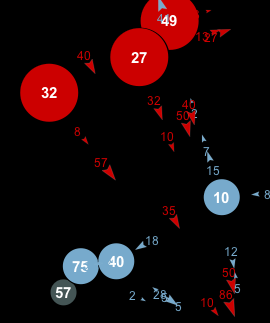
\includegraphics[height=0.5\textwidth]{pw_screenshot}}
	\hspace{0.5cm}
	\subfloat[Flash игра ``Galcon'' на офциальном сайте]{\label{fig:galcon_screenshot}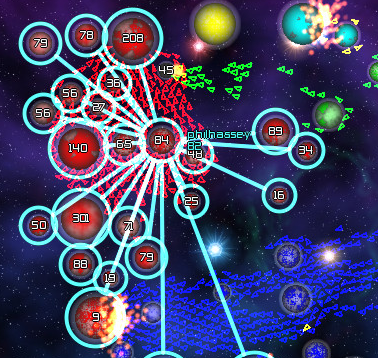
\includegraphics[height=0.5\textwidth]{galcon_screenshot}}
	\caption{Фрагменты игр ``Войны планет'' \subref{fig:pw_contest_screenshot} и ``Galcon'' \subref{fig:galcon_screenshot}}
	\label{fig:pw_screenshot}
\end{figure}



\subsection{Сущности игры}
ВП представляют собой 2D холст или карту, где происходит сама игра, на котором действуют следующие сущности (рис. \ref{fig:pw_entities}):
\begin{description}
\item[Планета]\hfill \\
	\emph{Планета} может
	\begin{myItemize}
	\item принадлежать одному из игроков или быть нейтральной;
	\item хранить, и если принадлежит кому-то, то и производить корабли с константной скоростью\footnote{\emph{Коэффициент роста} или просто \emph{рост} - это то, сколько кораблей будет появляться на планете за один ход. Обычно варьируется от 0 до 5.};
	\item выпускать корабли для атаки противника, захвата нейтральных планет или для перегруппировки;
	\item становиться чьей-то в случае нейтральности или менять хозяина в случае успешной атаки;	 
	\end{myItemize}
В начале игры все планеты располагаются на карте и до конца игры не меняют своего положения. \emph{Расстоянием} между планетами считается как округлённое геометрическое расстояние, рассчитанное по координатам планет. Планеты располагаются таким образом, что как бы делят карту на две симметричные половины. Все планеты кроме двух изначально нейтральные и обладают определённым количеством кораблей. У каждого участника в начале игры есть в наличии по одной планете с сотней кораблей.
\item[Флотилия и корабль]\hfill \\
\emph{Флотилия} - это группа кораблей, которые \emph{планета-источник} пустила по направлению к \emph{планете-цели}. Флотилия существует количество ходов, равное расстоянию между планетами источника и цели, перемещаясь за каждый ход на одну единицу\footnote{Имеется ввиду единица расстояния. Например, если расстояние между планетами равняется 5, то флотилия пролетает от одной до другой за 5 ходов.} по направлению к цели. С момента выпуска флотилии с ней ничего нельзя сделать: ни поменять направления, ни отменить решения. \emph{Корабль} - это разменная единица, из которых ``состоят'' флотилии и которые производят планеты участников.
\item[Выбор]\hfill \\
Решение, которое принимает ИИ игрока на каждом \emph{полу-ходу}\footnote{Это половинка всего хода, состоящая из решения одного из игроков} партии (см. \ref{sec:strategic}). Он состоит из набора новых флотилий, выпускаемых на этом ходу игроком.
\end{description}

\begin{figure}[h]
	\centering
	%LaTeX with PSTricks extensions
%%Creator: inkscape 0.48.0
%%Please note this file requires PSTricks extensions
\psset{xunit=.6pt,yunit=.6pt,runit=.6pt}
\begin{pspicture}(640,386)
{
\newrgbcolor{curcolor}{0.60000002 0.60000002 0.60000002}
\pscustom[linestyle=none,fillstyle=solid,fillcolor=curcolor]
{
\newpath
\moveto(96.10208,91.06372)
\lineto(96.10208,91.06372)
\lineto(102.539185,95.81384)
\lineto(103.132935,95.00922)
\lineto(96.69583,90.2591)
\closepath
\moveto(104.953094,97.59515)
\lineto(104.953094,97.59515)
\lineto(105.75774,98.18893)
\lineto(106.35149,97.3843)
\lineto(105.546844,96.79053)
\closepath
\moveto(108.171646,99.97025)
\lineto(108.171646,99.97025)
\lineto(114.60875,104.72037)
\lineto(115.2025,103.91574)
\lineto(108.765396,99.16562)
\closepath
\moveto(117.02266,106.50168)
\lineto(117.02266,106.50168)
\lineto(117.8273,107.09546)
\lineto(118.42105,106.29083)
\lineto(117.61641,105.69705)
\closepath
\moveto(120.24121,108.87677)
\lineto(120.24121,108.87677)
\lineto(126.678314,113.6269)
\lineto(127.272064,112.82227)
\lineto(120.83496,108.07214)
\closepath
\moveto(129.09222,115.4082)
\lineto(129.09222,115.4082)
\lineto(129.89688,116.00198)
\lineto(130.49063,115.19736)
\lineto(129.68597,114.60358)
\closepath
\moveto(132.31079,117.7833)
\lineto(132.31079,117.7833)
\lineto(138.7479,122.53342)
\lineto(139.34164,121.7288)
\lineto(132.90454,116.97867)
\closepath
\moveto(141.1618,124.31473)
\lineto(141.1618,124.31473)
\lineto(141.96646,124.9085)
\lineto(142.56021,124.10388)
\lineto(141.75555,123.5101)
\closepath
\moveto(144.38037,126.68982)
\lineto(144.38037,126.68982)
\lineto(150.81747,131.43994)
\lineto(151.41122,130.63531)
\lineto(144.97412,125.8852)
\closepath
\moveto(153.23138,133.22124)
\lineto(153.23138,133.22124)
\lineto(154.03604,133.81499)
\lineto(154.62979,133.01033)
\lineto(153.82513,132.41658)
\closepath
\moveto(156.44995,135.59625)
\lineto(156.44995,135.59625)
\lineto(162.88705,140.34637)
\lineto(163.4808,139.54175)
\lineto(157.0437,134.79163)
\closepath
\moveto(165.30096,142.12767)
\lineto(165.30096,142.12767)
\lineto(166.10562,142.72142)
\lineto(166.69937,141.91676)
\lineto(165.89471,141.32301)
\closepath
\moveto(168.51953,144.50269)
\lineto(168.51953,144.50269)
\lineto(174.95663,149.2528)
\lineto(175.55038,148.44818)
\lineto(169.11328,143.69806)
\closepath
\moveto(177.37054,151.0341)
\lineto(177.37054,151.0341)
\lineto(178.1752,151.62785)
\lineto(178.76895,150.8232)
\lineto(177.9643,150.22945)
\closepath
\moveto(180.58911,153.40912)
\lineto(180.58911,153.40912)
\lineto(187.02621,158.15924)
\lineto(187.61996,157.35461)
\lineto(181.18286,152.60449)
\closepath
\moveto(189.44012,159.94054)
\lineto(189.44012,159.94054)
\lineto(190.24478,160.53429)
\lineto(190.83853,159.72963)
\lineto(190.03387,159.13588)
\closepath
\moveto(192.65869,162.31555)
\lineto(192.65869,162.31555)
\lineto(199.0958,167.06567)
\lineto(199.68954,166.26105)
\lineto(193.25244,161.51093)
\closepath
\moveto(201.5097,168.84697)
\lineto(201.5097,168.84697)
\lineto(202.31436,169.44072)
\lineto(202.90811,168.63606)
\lineto(202.10345,168.04231)
\closepath
\moveto(204.72827,171.22198)
\lineto(204.72827,171.22198)
\lineto(211.16537,175.9721)
\lineto(211.75912,175.16748)
\lineto(205.32202,170.41736)
\closepath
\moveto(213.57928,177.7534)
\lineto(213.57928,177.7534)
\lineto(214.38394,178.34715)
\lineto(214.97769,177.5425)
\lineto(214.17303,176.94875)
\closepath
\moveto(216.79785,180.12842)
\lineto(216.79785,180.12842)
\lineto(223.23495,184.87854)
\lineto(223.8287,184.07391)
\lineto(217.3916,179.32379)
\closepath
\moveto(225.64886,186.65984)
\lineto(225.64886,186.65984)
\lineto(226.45352,187.25359)
\lineto(227.04727,186.44893)
\lineto(226.24261,185.85518)
\closepath
\moveto(228.86743,189.03485)
\lineto(228.86743,189.03485)
\lineto(235.30453,193.78497)
\lineto(235.89828,192.98035)
\lineto(229.46118,188.23022)
\closepath
\moveto(237.71844,195.56627)
\lineto(237.71844,195.56627)
\lineto(238.5231,196.16002)
\lineto(239.11685,195.35536)
\lineto(238.3122,194.76161)
\closepath
\moveto(240.93701,197.94128)
\lineto(240.93701,197.94128)
\lineto(247.37411,202.6914)
\lineto(247.96786,201.88678)
\lineto(241.53076,197.13666)
\closepath
\moveto(249.78802,204.4727)
\lineto(249.78802,204.4727)
\lineto(250.59268,205.06645)
\lineto(251.18643,204.2618)
\lineto(250.38177,203.66805)
\closepath
\moveto(253.00659,206.84775)
\lineto(253.00659,206.84775)
\lineto(259.4437,211.59787)
\lineto(260.03745,210.79324)
\lineto(253.60034,206.04312)
\closepath
\moveto(261.8576,213.37918)
\lineto(261.8576,213.37918)
\lineto(262.66223,213.97293)
\lineto(263.25598,213.1683)
\lineto(262.45135,212.57455)
\closepath
\moveto(265.07614,215.75424)
\lineto(265.07614,215.75424)
\lineto(271.51324,220.50436)
\lineto(272.107,219.69974)
\lineto(265.6699,214.94962)
\closepath
\moveto(273.92715,222.28568)
\lineto(273.92715,222.28568)
\lineto(274.73178,222.87943)
\lineto(275.32553,222.0748)
\lineto(274.5209,221.48105)
\closepath
\moveto(277.1457,224.66074)
\lineto(277.1457,224.66074)
\lineto(283.5828,229.41086)
\lineto(284.17654,228.60623)
\lineto(277.73944,223.85611)
\closepath
\moveto(285.9967,231.19217)
\lineto(285.9967,231.19217)
\lineto(286.80133,231.78592)
\lineto(287.39508,230.9813)
\lineto(286.59045,230.38754)
\closepath
\moveto(289.21524,233.56723)
\lineto(289.21524,233.56723)
\lineto(295.65234,238.31738)
\lineto(296.2461,237.51276)
\lineto(289.809,232.7626)
\closepath
\moveto(298.06625,240.0987)
\lineto(298.06625,240.0987)
\lineto(298.87088,240.69244)
\lineto(299.46463,239.88782)
\lineto(298.66,239.29407)
\closepath
\moveto(301.2848,242.47375)
\lineto(301.2848,242.47375)
\lineto(307.7219,247.2239)
\lineto(308.31564,246.41928)
\lineto(301.87854,241.66913)
\closepath
\moveto(310.1358,249.00522)
\lineto(310.1358,249.00522)
\lineto(310.94043,249.59897)
\lineto(311.53418,248.79434)
\lineto(310.72955,248.20059)
\closepath
\moveto(313.35434,251.38028)
\lineto(313.35434,251.38028)
\lineto(319.79144,256.13043)
\lineto(320.3852,255.3258)
\lineto(313.9481,250.57565)
\closepath
\moveto(322.20535,257.91174)
\lineto(322.20535,257.91174)
\lineto(323.00998,258.50551)
\lineto(323.60373,257.70088)
\lineto(322.7991,257.10712)
\closepath
\moveto(325.4239,260.286804)
\lineto(325.4239,260.286804)
\lineto(331.86096,265.03694)
\lineto(332.4547,264.232315)
\lineto(326.01764,259.48218)
\closepath
\moveto(334.27487,266.81824)
\lineto(334.27487,266.81824)
\lineto(335.0795,267.412)
\lineto(335.67325,266.607376)
\lineto(334.86862,266.01361)
\closepath
\moveto(337.4934,269.1933)
\lineto(337.4934,269.1933)
\lineto(343.93048,273.94345)
\lineto(344.52423,273.138824)
\lineto(338.08716,268.38867)
\closepath
\moveto(346.3444,275.72475)
\lineto(346.3444,275.72475)
\lineto(347.14902,276.31851)
\lineto(347.74277,275.513885)
\lineto(346.93814,274.92012)
\closepath
\moveto(349.56293,278.09981)
\lineto(349.56293,278.09981)
\lineto(356,282.84996)
\lineto(356.59375,282.045334)
\lineto(350.15668,277.29518)
\closepath
\moveto(358.4139,284.631256)
\lineto(358.4139,284.631256)
\lineto(359.21854,285.22502)
\lineto(359.8123,284.420395)
\lineto(359.00766,283.82663)
\closepath
\moveto(361.63245,287.00632)
\lineto(361.63245,287.00632)
\lineto(368.06952,291.75647)
\lineto(368.66327,290.95184)
\lineto(362.2262,286.20169)
\closepath
\moveto(370.48343,293.537766)
\lineto(370.48343,293.537766)
\lineto(371.28806,294.13153)
\lineto(371.8818,293.326904)
\lineto(371.07718,292.73314)
\closepath
\moveto(373.70197,295.91284)
\lineto(373.70197,295.91284)
\lineto(376.60602,298.05585)
\lineto(377.19977,297.25122)
\lineto(374.29572,295.108215)
\closepath
}
}
{
\newrgbcolor{curcolor}{0.60000002 0.60000002 0.60000002}
\pscustom[linestyle=none,fillstyle=solid,fillcolor=curcolor]
{
\newpath
\moveto(234.25342,48.18304)
\lineto(234.25342,48.18304)
\lineto(226.59985,50.51178)
\lineto(226.89093,51.4685)
\lineto(234.5445,49.13977)
\closepath
\moveto(223.72975,51.38507)
\lineto(223.72975,51.38507)
\lineto(222.77306,51.6762)
\lineto(223.06416,52.63287)
\lineto(224.02086,52.3418)
\closepath
\moveto(219.90298,52.5495)
\lineto(219.90298,52.5495)
\lineto(212.24942,54.87823)
\lineto(212.5405,55.8349)
\lineto(220.19406,53.50616)
\closepath
\moveto(209.37932,55.75146)
\lineto(209.37932,55.75146)
\lineto(208.42262,56.0426)
\lineto(208.71373,56.99927)
\lineto(209.67043,56.7082)
\closepath
\moveto(205.55255,56.91583)
\lineto(205.55255,56.91583)
\lineto(197.89899,59.24457)
\lineto(198.19006,60.2013)
\lineto(205.84363,57.87256)
\closepath
\moveto(195.0289,60.11786)
\lineto(195.0289,60.11786)
\lineto(194.0722,60.40894)
\lineto(194.36328,61.36566)
\lineto(195.31998,61.0746)
\closepath
\moveto(191.20212,61.28223)
\lineto(191.20212,61.28223)
\lineto(183.54855,63.61096)
\lineto(183.83963,64.5677)
\lineto(191.4932,62.23895)
\closepath
\moveto(180.67845,64.48425)
\lineto(180.67845,64.48425)
\lineto(179.72176,64.77533)
\lineto(180.01286,65.73206)
\lineto(180.96956,65.44092)
\closepath
\moveto(176.85168,65.64862)
\lineto(176.85168,65.64862)
\lineto(169.19812,67.97736)
\lineto(169.4892,68.93402)
\lineto(177.14276,66.6053)
\closepath
\moveto(166.32803,68.85065)
\lineto(166.32803,68.85065)
\lineto(165.37134,69.14172)
\lineto(165.66241,70.0984)
\lineto(166.61911,69.8073)
\closepath
\moveto(162.50125,70.015)
\lineto(162.50125,70.015)
\lineto(154.84769,72.34375)
\lineto(155.13876,73.3004)
\lineto(162.79233,70.97168)
\closepath
\moveto(151.97758,73.21698)
\lineto(151.97758,73.21698)
\lineto(151.02089,73.50812)
\lineto(151.312,74.46478)
\lineto(152.26869,74.1737)
\closepath
\moveto(148.15082,74.38135)
\lineto(148.15082,74.38135)
\lineto(140.49725,76.71008)
\lineto(140.78833,77.6668)
\lineto(148.4419,75.33807)
\closepath
\moveto(137.62717,77.58337)
\lineto(137.62717,77.58337)
\lineto(136.67047,77.87445)
\lineto(136.96155,78.83118)
\lineto(137.91824,78.5401)
\closepath
\moveto(133.80038,78.74774)
\lineto(133.80038,78.74774)
\lineto(126.14682,81.07648)
\lineto(126.4379,82.0332)
\lineto(134.09146,79.70447)
\closepath
\moveto(123.27672,81.94977)
\lineto(123.27672,81.94977)
\lineto(122.32002,82.24084)
\lineto(122.61113,83.19757)
\lineto(123.567825,82.90643)
\closepath
\moveto(119.44995,83.11414)
\lineto(119.44995,83.11414)
\lineto(111.7964,85.44287)
\lineto(112.08748,86.39954)
\lineto(119.74103,84.0708)
\closepath
\moveto(108.926315,86.31616)
\lineto(108.926315,86.31616)
\lineto(107.96962,86.60724)
\lineto(108.2607,87.5639)
\lineto(109.21739,87.27283)
\closepath
\moveto(105.09953,87.48053)
\lineto(105.09953,87.48053)
\lineto(97.44597,89.80927)
\lineto(97.737045,90.76593)
\lineto(105.39061,88.4372)
\closepath
}
}
{
\newrgbcolor{curcolor}{0.60000002 0.60000002 0.60000002}
\pscustom[linestyle=none,fillstyle=solid,fillcolor=curcolor]
{
\newpath
\moveto(377.37167,297.49478)
\lineto(377.37167,297.49478)
\lineto(374.70547,289.95215)
\lineto(373.76266,290.2854)
\lineto(376.42886,297.82803)
\closepath
\moveto(373.70566,287.12366)
\lineto(373.70566,287.12366)
\lineto(373.37238,286.18082)
\lineto(372.42957,286.51407)
\lineto(372.76285,287.45691)
\closepath
\moveto(372.37256,283.352325)
\lineto(372.37256,283.352325)
\lineto(369.70636,275.80969)
\lineto(368.76355,276.142944)
\lineto(371.42975,283.68558)
\closepath
\moveto(368.70654,272.9812)
\lineto(368.70654,272.9812)
\lineto(368.37326,272.03836)
\lineto(367.43045,272.37161)
\lineto(367.76373,273.31445)
\closepath
\moveto(367.37344,269.20987)
\lineto(367.37344,269.20987)
\lineto(364.70724,261.66724)
\lineto(363.76443,262.00049)
\lineto(366.43063,269.54312)
\closepath
\moveto(363.70743,258.838745)
\lineto(363.70743,258.838745)
\lineto(363.37415,257.8959)
\lineto(362.43134,258.22916)
\lineto(362.76462,259.172)
\closepath
\moveto(362.37433,255.06741)
\lineto(362.37433,255.06741)
\lineto(359.70813,247.52478)
\lineto(358.76532,247.85803)
\lineto(361.43152,255.40067)
\closepath
\moveto(358.7083,244.69629)
\lineto(358.7083,244.69629)
\lineto(358.37503,243.75345)
\lineto(357.43222,244.0867)
\lineto(357.7655,245.02954)
\closepath
\moveto(357.3752,240.92496)
\lineto(357.3752,240.92496)
\lineto(354.709,233.38232)
\lineto(353.7662,233.71558)
\lineto(356.4324,241.25821)
\closepath
\moveto(353.7092,230.55383)
\lineto(353.7092,230.55383)
\lineto(353.37592,229.611)
\lineto(352.4331,229.94424)
\lineto(352.7664,230.88708)
\closepath
\moveto(352.3761,226.7825)
\lineto(352.3761,226.7825)
\lineto(349.7099,219.23987)
\lineto(348.7671,219.57312)
\lineto(351.4333,227.11575)
\closepath
\moveto(348.71008,216.41138)
\lineto(348.71008,216.41138)
\lineto(348.3768,215.46854)
\lineto(347.434,215.80179)
\lineto(347.76727,216.74463)
\closepath
\moveto(347.37698,212.64005)
\lineto(347.37698,212.64005)
\lineto(344.7108,205.09741)
\lineto(343.76797,205.43066)
\lineto(346.43417,212.9733)
\closepath
\moveto(343.71097,202.26892)
\lineto(343.71097,202.26892)
\lineto(343.3777,201.32608)
\lineto(342.43488,201.65933)
\lineto(342.76816,202.60217)
\closepath
\moveto(342.37787,198.49759)
\lineto(342.37787,198.49759)
\lineto(339.71164,190.95496)
\lineto(338.76883,191.28821)
\lineto(341.43506,198.83084)
\closepath
\moveto(338.71182,188.12646)
\lineto(338.71182,188.12646)
\lineto(338.37854,187.18362)
\lineto(337.43573,187.51688)
\lineto(337.769,188.45972)
\closepath
\moveto(337.37872,184.35513)
\lineto(337.37872,184.35513)
\lineto(334.7125,176.8125)
\lineto(333.76968,177.14575)
\lineto(336.4359,184.68839)
\closepath
\moveto(333.71268,173.98401)
\lineto(333.71268,173.98401)
\lineto(333.3794,173.04117)
\lineto(332.43658,173.37442)
\lineto(332.76987,174.31726)
\closepath
\moveto(332.37958,170.21268)
\lineto(332.37958,170.21268)
\lineto(329.71335,162.67004)
\lineto(328.77054,163.0033)
\lineto(331.43677,170.54593)
\closepath
\moveto(328.71353,159.84155)
\lineto(328.71353,159.84155)
\lineto(328.38025,158.89871)
\lineto(327.43744,159.23196)
\lineto(327.77072,160.1748)
\closepath
\moveto(327.3804,156.07022)
\lineto(327.3804,156.07022)
\lineto(324.71417,148.52759)
\lineto(323.77136,148.86084)
\lineto(326.4376,156.40347)
\closepath
\moveto(323.71436,145.6991)
\lineto(323.71436,145.6991)
\lineto(323.38107,144.75626)
\lineto(322.43826,145.08951)
\lineto(322.77155,146.03235)
\closepath
\moveto(322.38126,141.92776)
\lineto(322.38126,141.92776)
\lineto(319.71503,134.38513)
\lineto(318.77222,134.71838)
\lineto(321.43845,142.26102)
\closepath
\moveto(318.71518,131.55664)
\lineto(318.71518,131.55664)
\lineto(318.3819,130.6138)
\lineto(317.4391,130.94705)
\lineto(317.77237,131.8899)
\closepath
\moveto(317.38208,127.7853)
\lineto(317.38208,127.7853)
\lineto(315.85986,123.47903)
\lineto(314.91705,123.8123)
\lineto(316.43927,128.11856)
\closepath
}
}
{
\newrgbcolor{curcolor}{0.60000002 0.60000002 0.60000002}
\pscustom[linestyle=none,fillstyle=solid,fillcolor=curcolor]
{
\newpath
\moveto(372.47815,294.167725)
\lineto(372.47815,294.167725)
\lineto(364.57916,292.90039)
\lineto(364.42078,293.88776)
\lineto(372.31976,295.15509)
\closepath
\moveto(361.61707,292.42514)
\lineto(361.61707,292.42514)
\lineto(360.6297,292.26672)
\lineto(360.47125,293.25409)
\lineto(361.45862,293.412506)
\closepath
\moveto(357.66754,291.79147)
\lineto(357.66754,291.79147)
\lineto(349.76855,290.52414)
\lineto(349.61017,291.511505)
\lineto(357.50916,292.77884)
\closepath
\moveto(346.80646,290.04889)
\lineto(346.80646,290.04889)
\lineto(345.8191,289.89047)
\lineto(345.66064,290.87784)
\lineto(346.648,291.036255)
\closepath
\moveto(342.85693,289.41522)
\lineto(342.85693,289.41522)
\lineto(334.95795,288.14789)
\lineto(334.79956,289.135254)
\lineto(342.69855,290.40259)
\closepath
\moveto(331.99585,287.67264)
\lineto(331.99585,287.67264)
\lineto(331.00848,287.51422)
\lineto(330.85004,288.50159)
\lineto(331.8374,288.66)
\closepath
\moveto(328.04633,287.03897)
\lineto(328.04633,287.03897)
\lineto(320.14734,285.77164)
\lineto(319.98895,286.759)
\lineto(327.88794,288.02634)
\closepath
\moveto(317.18524,285.29639)
\lineto(317.18524,285.29639)
\lineto(316.19788,285.13797)
\lineto(316.03943,286.125336)
\lineto(317.0268,286.28375)
\closepath
\moveto(313.23572,284.66272)
\lineto(313.23572,284.66272)
\lineto(305.33673,283.395386)
\lineto(305.17834,284.38275)
\lineto(313.07733,285.650085)
\closepath
\moveto(302.37463,282.920135)
\lineto(302.37463,282.920135)
\lineto(301.38727,282.76172)
\lineto(301.22882,283.749084)
\lineto(302.2162,283.9075)
\closepath
\moveto(298.4251,282.28647)
\lineto(298.4251,282.28647)
\lineto(290.52612,281.019135)
\lineto(290.36774,282.0065)
\lineto(298.26672,283.273834)
\closepath
\moveto(287.56403,280.543884)
\lineto(287.56403,280.543884)
\lineto(286.57666,280.38547)
\lineto(286.4182,281.37283)
\lineto(287.40558,281.53125)
\closepath
\moveto(283.6145,279.91022)
\lineto(283.6145,279.91022)
\lineto(275.7155,278.64288)
\lineto(275.55713,279.63025)
\lineto(283.45612,280.89758)
\closepath
\moveto(272.75342,278.16763)
\lineto(272.75342,278.16763)
\lineto(271.76605,278.00922)
\lineto(271.6076,278.99658)
\lineto(272.59497,279.155)
\closepath
\moveto(268.8039,277.533966)
\lineto(268.8039,277.533966)
\lineto(260.9049,276.26663)
\lineto(260.74652,277.254)
\lineto(268.6455,278.52133)
\closepath
\moveto(257.9428,275.79138)
\lineto(257.9428,275.79138)
\lineto(256.95544,275.632965)
\lineto(256.797,276.62033)
\lineto(257.78436,276.77875)
\closepath
\moveto(253.99332,275.157715)
\lineto(253.99332,275.157715)
\lineto(246.09433,273.89038)
\lineto(245.93594,274.87775)
\lineto(253.83493,276.14508)
\closepath
\moveto(243.13225,273.41513)
\lineto(243.13225,273.41513)
\lineto(242.14488,273.256714)
\lineto(241.98647,274.24408)
\lineto(242.97383,274.4025)
\closepath
\moveto(239.18277,272.78146)
\lineto(239.18277,272.78146)
\lineto(231.28378,271.51413)
\lineto(231.1254,272.501495)
\lineto(239.02438,273.76883)
\closepath
\moveto(228.3217,271.03888)
\lineto(228.3217,271.03888)
\lineto(227.33434,270.88046)
\lineto(227.17592,271.86783)
\lineto(228.16328,272.026245)
\closepath
\moveto(224.37222,270.40521)
\lineto(224.37222,270.40521)
\lineto(216.47324,269.13788)
\lineto(216.31485,270.125244)
\lineto(224.21384,271.39258)
\closepath
\moveto(213.51115,268.66263)
\lineto(213.51115,268.66263)
\lineto(212.52379,268.50421)
\lineto(212.36537,269.49158)
\lineto(213.35274,269.649994)
\closepath
\moveto(209.56168,268.02896)
\lineto(209.56168,268.02896)
\lineto(201.66269,266.76164)
\lineto(201.5043,267.74901)
\lineto(209.40329,269.01633)
\closepath
\moveto(198.7006,266.28639)
\lineto(198.7006,266.28639)
\lineto(197.71324,266.127975)
\lineto(197.55482,267.11534)
\lineto(198.54219,267.27376)
\closepath
\moveto(194.75113,265.652725)
\lineto(194.75113,265.652725)
\lineto(186.85214,264.38541)
\lineto(186.69376,265.37277)
\lineto(194.59274,266.64009)
\closepath
\moveto(183.89006,263.91017)
\lineto(183.89006,263.91017)
\lineto(182.9027,263.751755)
\lineto(182.74428,264.73912)
\lineto(183.73164,264.89754)
\closepath
\moveto(179.94058,263.27652)
\lineto(179.94058,263.27652)
\lineto(175.97421,262.64017)
\lineto(175.81583,263.62753)
\lineto(179.7822,264.263885)
\closepath
}
}
{
\newrgbcolor{curcolor}{0.02745098 0.21568628 0.3882353}
\pscustom[linestyle=none,fillstyle=solid,fillcolor=curcolor]
{
\newpath
\moveto(27.952362,337.49388)
\lineto(27.952362,337.49388)
\lineto(29.619919,336.38968)
\lineto(28.515732,334.722137)
\lineto(26.848175,335.82634)
\closepath
\moveto(34.622574,333.077057)
\lineto(34.622574,333.077057)
\lineto(36.29013,331.972855)
\lineto(35.185944,330.305313)
\lineto(33.518387,331.409515)
\closepath
\moveto(41.292786,328.660233)
\lineto(41.292786,328.660233)
\lineto(42.960342,327.55603)
\lineto(41.856155,325.88849)
\lineto(40.1886,326.99269)
\closepath
\moveto(47.962997,324.24341)
\lineto(47.962997,324.24341)
\lineto(49.630554,323.139206)
\lineto(48.526367,321.471664)
\lineto(46.85881,322.575867)
\closepath
\moveto(54.63321,319.826584)
\lineto(54.63321,319.826584)
\lineto(56.300766,318.72238)
\lineto(55.19658,317.05484)
\lineto(53.529022,318.15904)
\closepath
\moveto(61.30342,315.40976)
\lineto(61.30342,315.40976)
\lineto(62.970978,314.30556)
\lineto(61.86679,312.638016)
\lineto(60.199234,313.74222)
\closepath
\moveto(67.97363,310.992935)
\lineto(67.97363,310.992935)
\lineto(69.64119,309.88873)
\lineto(68.537,308.22119)
\lineto(66.869446,309.32539)
\closepath
\moveto(74.643845,306.57611)
\lineto(74.643845,306.57611)
\lineto(76.3114,305.47191)
\lineto(75.207214,303.80437)
\lineto(73.53966,304.90857)
\closepath
\moveto(81.31406,302.15929)
\lineto(81.31406,302.15929)
\lineto(82.98161,301.055084)
\lineto(81.877426,299.38754)
\lineto(80.20987,300.491745)
\closepath
\moveto(87.98427,297.74246)
\lineto(87.98427,297.74246)
\lineto(89.651825,296.63826)
\lineto(88.54764,294.97072)
\lineto(86.88008,296.07492)
\closepath
\moveto(94.65448,293.32564)
\lineto(94.65448,293.32564)
\lineto(96.32204,292.221436)
\lineto(95.21785,290.553894)
\lineto(93.55029,291.6581)
\closepath
\moveto(101.32469,288.90881)
\lineto(101.32469,288.90881)
\lineto(102.99225,287.80461)
\lineto(101.88806,286.13707)
\lineto(100.220505,287.24127)
\closepath
\moveto(107.9949,284.49199)
\lineto(107.9949,284.49199)
\lineto(109.66246,283.38779)
\lineto(108.55827,281.720245)
\lineto(106.89072,282.82445)
\closepath
\moveto(114.66513,280.075165)
\lineto(114.66513,280.075165)
\lineto(116.33269,278.97096)
\lineto(115.2285,277.30342)
\lineto(113.56094,278.40762)
\closepath
\moveto(121.33534,275.65834)
\lineto(121.33534,275.65834)
\lineto(123.0029,274.55414)
\lineto(121.89871,272.8866)
\lineto(120.231155,273.9908)
\closepath
\moveto(128.00555,271.241516)
\lineto(128.00555,271.241516)
\lineto(129.67313,270.137314)
\lineto(128.56894,268.46977)
\lineto(126.90137,269.573975)
\closepath
\moveto(134.67578,266.82469)
\lineto(134.67578,266.82469)
\lineto(136.34335,265.72049)
\lineto(135.23917,264.05295)
\lineto(133.5716,265.15715)
\closepath
\moveto(141.34601,262.40787)
\lineto(141.34601,262.40787)
\lineto(143.01358,261.303665)
\lineto(141.9094,259.63612)
\lineto(140.24182,260.740326)
\closepath
\moveto(148.01624,257.99106)
\lineto(148.01624,257.99106)
\lineto(149.6838,256.88684)
\lineto(148.57962,255.2193)
\lineto(146.91205,256.32352)
\closepath
\moveto(154.68646,253.57422)
\lineto(154.68646,253.57422)
\lineto(156.35403,252.47)
\lineto(155.24985,250.80246)
\lineto(153.58228,251.90668)
\closepath
\moveto(161.35669,249.15738)
\lineto(161.35669,249.15738)
\lineto(163.02426,248.05316)
\lineto(161.92007,246.38562)
\lineto(160.2525,247.48984)
\closepath
\moveto(168.02692,244.74054)
\lineto(168.02692,244.74054)
\lineto(169.69449,243.63632)
\lineto(168.5903,241.96878)
\lineto(166.92273,243.073)
\closepath
\moveto(174.69714,240.3237)
\lineto(174.69714,240.3237)
\lineto(176.36472,239.21948)
\lineto(175.26053,237.55194)
\lineto(173.59296,238.65616)
\closepath
\moveto(181.36737,235.90686)
\lineto(181.36737,235.90686)
\lineto(183.03494,234.80264)
\lineto(181.93076,233.1351)
\lineto(180.26318,234.23932)
\closepath
\moveto(188.0376,231.49002)
\lineto(188.0376,231.49002)
\lineto(189.70517,230.3858)
\lineto(188.60098,228.71826)
\lineto(186.93341,229.82248)
\closepath
\moveto(194.70782,227.07318)
\lineto(194.70782,227.07318)
\lineto(196.3754,225.96896)
\lineto(195.27121,224.30142)
\lineto(193.60364,225.40564)
\closepath
\moveto(201.37805,222.65634)
\lineto(201.37805,222.65634)
\lineto(203.04562,221.55212)
\lineto(201.94144,219.88458)
\lineto(200.27386,220.9888)
\closepath
\moveto(208.04828,218.2395)
\lineto(208.04828,218.2395)
\lineto(209.71585,217.13528)
\lineto(208.61166,215.46774)
\lineto(206.94409,216.57196)
\closepath
\moveto(214.7185,213.82266)
\lineto(214.7185,213.82266)
\lineto(216.38608,212.71844)
\lineto(215.28189,211.0509)
\lineto(213.61432,212.15512)
\closepath
\moveto(221.38873,209.40582)
\lineto(221.38873,209.40582)
\lineto(223.0563,208.3016)
\lineto(221.95212,206.63406)
\lineto(220.28455,207.73828)
\closepath
\moveto(228.05896,204.98898)
\lineto(228.05896,204.98898)
\lineto(229.72653,203.88477)
\lineto(228.62234,202.21722)
\lineto(226.95477,203.32144)
\closepath
\moveto(234.72919,200.57214)
\lineto(234.72919,200.57214)
\lineto(236.39676,199.46793)
\lineto(235.29257,197.80038)
\lineto(233.625,198.9046)
\closepath
\moveto(241.39941,196.1553)
\lineto(241.39941,196.1553)
\lineto(243.06699,195.05109)
\lineto(241.9628,193.38354)
\lineto(240.29523,194.48776)
\closepath
\moveto(248.06964,191.73846)
\lineto(248.06964,191.73846)
\lineto(249.73721,190.63425)
\lineto(248.63303,188.9667)
\lineto(246.96545,190.07092)
\closepath
\moveto(254.73987,187.32162)
\lineto(254.73987,187.32162)
\lineto(256.40744,186.2174)
\lineto(255.30325,184.54987)
\lineto(253.63568,185.65408)
\closepath
\moveto(261.4101,182.90479)
\lineto(261.4101,182.90479)
\lineto(263.07764,181.80057)
\lineto(261.97345,180.13303)
\lineto(260.3059,181.23724)
\closepath
\moveto(268.08032,178.48795)
\lineto(268.08032,178.48795)
\lineto(269.74786,177.38373)
\lineto(268.64362,175.71619)
\lineto(266.97607,176.8204)
\closepath
\moveto(274.7505,174.0711)
\lineto(274.7505,174.0711)
\lineto(276.41803,172.96689)
\lineto(275.31384,171.29935)
\lineto(273.6463,172.40356)
\closepath
\moveto(281.42072,169.65427)
\lineto(281.42072,169.65427)
\lineto(283.08826,168.55005)
\lineto(281.984,166.8825)
\lineto(280.31647,167.98672)
\closepath
\moveto(288.09088,165.23743)
\lineto(288.09088,165.23743)
\lineto(289.75842,164.13321)
\lineto(288.65424,162.46567)
\lineto(286.9867,163.56989)
\closepath
\moveto(294.7611,160.82059)
\lineto(294.7611,160.82059)
\lineto(296.42865,159.71637)
\lineto(295.3244,158.04883)
\lineto(293.65686,159.15305)
\closepath
\moveto(301.43127,156.40375)
\lineto(301.43127,156.40375)
\lineto(303.09882,155.29953)
\lineto(301.99463,153.63199)
\lineto(300.3271,154.7362)
\closepath
\moveto(308.1015,151.98691)
\lineto(308.1015,151.98691)
\lineto(309.76904,150.88269)
\lineto(308.6648,149.21515)
\lineto(306.99725,150.31937)
\closepath
\moveto(314.77167,147.57007)
\lineto(314.77167,147.57007)
\lineto(316.4392,146.46585)
\lineto(315.33502,144.79831)
\lineto(313.66748,145.90253)
\closepath
\moveto(321.4419,143.15323)
\lineto(321.4419,143.15323)
\lineto(323.10944,142.04901)
\lineto(322.0052,140.38147)
\lineto(320.33765,141.48569)
\closepath
\moveto(328.11206,138.73639)
\lineto(328.11206,138.73639)
\lineto(329.7796,137.63217)
\lineto(328.6754,135.96463)
\lineto(327.00787,137.06885)
\closepath
\moveto(334.7823,134.31955)
\lineto(334.7823,134.31955)
\lineto(336.44983,133.21533)
\lineto(335.34558,131.54779)
\lineto(333.67804,132.65201)
\closepath
\moveto(341.45245,129.90274)
\lineto(341.45245,129.90274)
\lineto(343.12,128.79855)
\lineto(342.0158,127.131)
\lineto(340.34827,128.2352)
\closepath
\moveto(348.12265,125.48596)
\lineto(348.12265,125.48596)
\lineto(349.7902,124.38177)
\lineto(348.686,122.71423)
\lineto(347.01846,123.81842)
\closepath
\moveto(354.79285,121.06918)
\lineto(354.79285,121.06918)
\lineto(356.4604,119.965)
\lineto(355.3562,118.29745)
\lineto(353.68866,119.40164)
\closepath
\moveto(361.46304,116.6524)
\lineto(361.46304,116.6524)
\lineto(363.13058,115.54822)
\lineto(362.0264,113.88068)
\lineto(360.35886,114.98486)
\closepath
\moveto(368.13324,112.23563)
\lineto(368.13324,112.23563)
\lineto(369.80078,111.13144)
\lineto(368.6966,109.4639)
\lineto(367.02905,110.56808)
\closepath
\moveto(374.80344,107.81885)
\lineto(374.80344,107.81885)
\lineto(376.47098,106.71466)
\lineto(375.3668,105.04712)
\lineto(373.69925,106.1513)
\closepath
\moveto(381.47363,103.40207)
\lineto(381.47363,103.40207)
\lineto(383.14117,102.29788)
\lineto(382.037,100.63034)
\lineto(380.36945,101.73453)
\closepath
\moveto(388.14383,98.9853)
\lineto(388.14383,98.9853)
\lineto(389.81137,97.8811)
\lineto(388.70718,96.21356)
\lineto(387.03964,97.31775)
\closepath
\moveto(394.81403,94.5685)
\lineto(394.81403,94.5685)
\lineto(396.48157,93.46432)
\lineto(395.37738,91.79678)
\lineto(393.70984,92.90097)
\closepath
\moveto(401.48422,90.15173)
\lineto(401.48422,90.15173)
\lineto(403.15176,89.04755)
\lineto(402.04758,87.38)
\lineto(400.38004,88.4842)
\closepath
\moveto(408.15442,85.73495)
\lineto(408.15442,85.73495)
\lineto(409.82196,84.63077)
\lineto(408.71777,82.96323)
\lineto(407.05023,84.0674)
\closepath
\moveto(414.82462,81.31818)
\lineto(414.82462,81.31818)
\lineto(416.49216,80.214)
\lineto(415.38797,78.54645)
\lineto(413.72043,79.65063)
\closepath
\moveto(421.4948,76.9014)
\lineto(421.4948,76.9014)
\lineto(423.16235,75.7972)
\lineto(422.05817,74.12967)
\lineto(420.39062,75.23386)
\closepath
\moveto(428.165,72.48462)
\lineto(428.165,72.48462)
\lineto(429.83255,71.38043)
\lineto(428.72836,69.7129)
\lineto(427.06082,70.81708)
\closepath
\moveto(434.8352,68.06784)
\lineto(434.8352,68.06784)
\lineto(436.50275,66.96365)
\lineto(435.39856,65.2961)
\lineto(433.73102,66.4003)
\closepath
\moveto(441.5054,63.65106)
\lineto(441.5054,63.65106)
\lineto(443.17294,62.54688)
\lineto(442.06876,60.87933)
\lineto(440.4012,61.98352)
\closepath
\moveto(448.1756,59.23428)
\lineto(448.1756,59.23428)
\lineto(449.84314,58.1301)
\lineto(448.73895,56.46255)
\lineto(447.0714,57.56674)
\closepath
\moveto(454.8458,54.8175)
\lineto(454.8458,54.8175)
\lineto(456.51334,53.71332)
\lineto(455.40915,52.04578)
\lineto(453.7416,53.14996)
\closepath
\moveto(461.516,50.40073)
\lineto(461.516,50.40073)
\lineto(463.18353,49.29654)
\lineto(462.07935,47.629)
\lineto(460.4118,48.7332)
\closepath
\moveto(468.1862,45.98392)
\lineto(468.1862,45.98392)
\lineto(469.85373,44.87973)
\lineto(468.74954,43.2122)
\lineto(467.082,44.31638)
\closepath
\moveto(474.85638,41.56714)
\lineto(474.85638,41.56714)
\lineto(476.52393,40.46295)
\lineto(475.41974,38.7954)
\lineto(473.7522,39.8996)
\closepath
}
}
{
\newrgbcolor{curcolor}{0.80000001 0.80000001 0.80000001}
\pscustom[linestyle=none,fillstyle=solid,fillcolor=curcolor]
{
\newpath
\moveto(49.893707,92.90945)
\lineto(49.893707,92.90945)
\curveto(49.893707,118.17538)(70.37579,138.65749)(95.64174,138.65749)
\lineto(95.64174,138.65749)
\curveto(107.774864,138.65749)(119.41106,133.83762)(127.99048,125.25818)
\curveto(136.5699,116.67877)(141.38977,105.04257)(141.38977,92.90945)
\lineto(141.38977,92.90945)
\curveto(141.38977,67.64352)(120.90768,47.1614)(95.64174,47.1614)
\lineto(95.64174,47.1614)
\curveto(70.37579,47.1614)(49.893707,67.64352)(49.893707,92.90945)
\closepath
}
}
{
\newrgbcolor{curcolor}{0.02745098 0.21568628 0.3882353}
\pscustom[linewidth=2,linecolor=curcolor]
{
\newpath
\moveto(49.893707,92.90945)
\lineto(49.893707,92.90945)
\curveto(49.893707,118.17538)(70.37579,138.65749)(95.64174,138.65749)
\lineto(95.64174,138.65749)
\curveto(107.774864,138.65749)(119.41106,133.83762)(127.99048,125.25818)
\curveto(136.5699,116.67877)(141.38977,105.04257)(141.38977,92.90945)
\lineto(141.38977,92.90945)
\curveto(141.38977,67.64352)(120.90768,47.1614)(95.64174,47.1614)
\lineto(95.64174,47.1614)
\curveto(70.37579,47.1614)(49.893707,67.64352)(49.893707,92.90945)
\closepath
}
}
{
\newrgbcolor{curcolor}{1 1 1}
\pscustom[linestyle=none,fillstyle=solid,fillcolor=curcolor]
{
\newpath
\moveto(10.904204,182.16798)
\lineto(10.904204,182.16798)
\curveto(10.904204,198.72783)(24.328611,212.15224)(40.88846,212.15224)
\lineto(40.88846,212.15224)
\curveto(48.840775,212.15224)(56.46739,208.99318)(62.090527,203.37004)
\curveto(67.71366,197.7469)(70.87271,190.1203)(70.87271,182.16798)
\lineto(70.87271,182.16798)
\curveto(70.87271,165.60814)(57.448303,152.18373)(40.88846,152.18373)
\lineto(40.88846,152.18373)
\curveto(24.328611,152.18373)(10.904204,165.60814)(10.904204,182.16798)
\closepath
}
}
{
\newrgbcolor{curcolor}{0.02745098 0.21568628 0.3882353}
\pscustom[linewidth=2,linecolor=curcolor]
{
\newpath
\moveto(10.904204,182.16798)
\lineto(10.904204,182.16798)
\curveto(10.904204,198.72783)(24.328611,212.15224)(40.88846,212.15224)
\lineto(40.88846,212.15224)
\curveto(48.840775,212.15224)(56.46739,208.99318)(62.090527,203.37004)
\curveto(67.71366,197.7469)(70.87271,190.1203)(70.87271,182.16798)
\lineto(70.87271,182.16798)
\curveto(70.87271,165.60814)(57.448303,152.18373)(40.88846,152.18373)
\lineto(40.88846,152.18373)
\curveto(24.328611,152.18373)(10.904204,165.60814)(10.904204,182.16798)
\closepath
}
}
{
\newrgbcolor{curcolor}{1 1 1}
\pscustom[linestyle=none,fillstyle=solid,fillcolor=curcolor]
{
\newpath
\moveto(282.89633,121.17715)
\lineto(282.89633,121.17715)
\curveto(282.89633,137.73701)(296.32074,151.16142)(312.88058,151.16142)
\lineto(312.88058,151.16142)
\curveto(320.8329,151.16142)(328.4595,148.00237)(334.08264,142.37923)
\curveto(339.70578,136.75609)(342.86484,129.1295)(342.86484,121.17715)
\lineto(342.86484,121.17715)
\curveto(342.86484,104.6173)(329.44043,91.1929)(312.88058,91.1929)
\lineto(312.88058,91.1929)
\curveto(296.32074,91.1929)(282.89633,104.6173)(282.89633,121.17715)
\closepath
}
}
{
\newrgbcolor{curcolor}{0.02745098 0.21568628 0.3882353}
\pscustom[linewidth=2,linecolor=curcolor]
{
\newpath
\moveto(282.89633,121.17715)
\lineto(282.89633,121.17715)
\curveto(282.89633,137.73701)(296.32074,151.16142)(312.88058,151.16142)
\lineto(312.88058,151.16142)
\curveto(320.8329,151.16142)(328.4595,148.00237)(334.08264,142.37923)
\curveto(339.70578,136.75609)(342.86484,129.1295)(342.86484,121.17715)
\lineto(342.86484,121.17715)
\curveto(342.86484,104.6173)(329.44043,91.1929)(312.88058,91.1929)
\lineto(312.88058,91.1929)
\curveto(296.32074,91.1929)(282.89633,104.6173)(282.89633,121.17715)
\closepath
}
}
{
\newrgbcolor{curcolor}{0.80000001 0.80000001 0.80000001}
\pscustom[linestyle=none,fillstyle=solid,fillcolor=curcolor]
{
\newpath
\moveto(215.89108,48.40945)
\lineto(215.89108,48.40945)
\curveto(215.89108,58.75934)(224.28133,67.1496)(234.63124,67.1496)
\lineto(234.63124,67.1496)
\curveto(239.60144,67.1496)(244.36807,65.1752)(247.88252,61.66074)
\curveto(251.39699,58.14627)(253.3714,53.37964)(253.3714,48.40945)
\lineto(253.3714,48.40945)
\curveto(253.3714,38.05954)(244.98114,29.66928)(234.63124,29.66928)
\lineto(234.63124,29.66928)
\curveto(224.28133,29.66928)(215.89108,38.05954)(215.89108,48.40945)
\closepath
}
}
{
\newrgbcolor{curcolor}{0.02745098 0.21568628 0.3882353}
\pscustom[linewidth=2,linecolor=curcolor]
{
\newpath
\moveto(215.89108,48.40945)
\lineto(215.89108,48.40945)
\curveto(215.89108,58.75934)(224.28133,67.1496)(234.63124,67.1496)
\lineto(234.63124,67.1496)
\curveto(239.60144,67.1496)(244.36807,65.1752)(247.88252,61.66074)
\curveto(251.39699,58.14627)(253.3714,53.37964)(253.3714,48.40945)
\lineto(253.3714,48.40945)
\curveto(253.3714,38.05954)(244.98114,29.66928)(234.63124,29.66928)
\lineto(234.63124,29.66928)
\curveto(224.28133,29.66928)(215.89108,38.05954)(215.89108,48.40945)
\closepath
}
}
{
\newrgbcolor{curcolor}{0.40000001 0.40000001 0.40000001}
\pscustom[linestyle=none,fillstyle=solid,fillcolor=curcolor]
{
\newpath
\moveto(419.36877,295.16929)
\lineto(419.36877,295.16929)
\curveto(419.36877,269.90335)(398.8867,249.42126)(373.62073,249.42126)
\lineto(373.62073,249.42126)
\curveto(361.4876,249.42126)(349.8514,254.24113)(341.272,262.82055)
\curveto(332.69257,271.39996)(327.8727,283.036156)(327.8727,295.16929)
\lineto(327.8727,295.16929)
\curveto(327.8727,320.43523)(348.3548,340.917316)(373.62073,340.917316)
\lineto(373.62073,340.917316)
\curveto(398.8867,340.917316)(419.36877,320.43523)(419.36877,295.16929)
\closepath
}
}
{
\newrgbcolor{curcolor}{0.02745098 0.21568628 0.3882353}
\pscustom[linewidth=2,linecolor=curcolor]
{
\newpath
\moveto(419.36877,295.16929)
\lineto(419.36877,295.16929)
\curveto(419.36877,269.90335)(398.8867,249.42126)(373.62073,249.42126)
\lineto(373.62073,249.42126)
\curveto(361.4876,249.42126)(349.8514,254.24113)(341.272,262.82055)
\curveto(332.69257,271.39996)(327.8727,283.036156)(327.8727,295.16929)
\lineto(327.8727,295.16929)
\curveto(327.8727,320.43523)(348.3548,340.917316)(373.62073,340.917316)
\lineto(373.62073,340.917316)
\curveto(398.8867,340.917316)(419.36877,320.43523)(419.36877,295.16929)
\closepath
}
}
{
\newrgbcolor{curcolor}{0.40000001 0.40000001 0.40000001}
\pscustom[linestyle=none,fillstyle=solid,fillcolor=curcolor]
{
\newpath
\moveto(458.35828,205.91077)
\lineto(458.35828,205.91077)
\curveto(458.35828,189.35092)(444.93387,175.92651)(428.37402,175.92651)
\lineto(428.37402,175.92651)
\curveto(420.4217,175.92651)(412.79507,179.08556)(407.17194,184.7087)
\curveto(401.5488,190.33183)(398.38977,197.95845)(398.38977,205.91077)
\lineto(398.38977,205.91077)
\curveto(398.38977,222.47061)(411.81418,235.89502)(428.37402,235.89502)
\lineto(428.37402,235.89502)
\curveto(444.93387,235.89502)(458.35828,222.47061)(458.35828,205.91077)
\closepath
}
}
{
\newrgbcolor{curcolor}{0.02745098 0.21568628 0.3882353}
\pscustom[linewidth=2,linecolor=curcolor]
{
\newpath
\moveto(458.35828,205.91077)
\lineto(458.35828,205.91077)
\curveto(458.35828,189.35092)(444.93387,175.92651)(428.37402,175.92651)
\lineto(428.37402,175.92651)
\curveto(420.4217,175.92651)(412.79507,179.08556)(407.17194,184.7087)
\curveto(401.5488,190.33183)(398.38977,197.95845)(398.38977,205.91077)
\lineto(398.38977,205.91077)
\curveto(398.38977,222.47061)(411.81418,235.89502)(428.37402,235.89502)
\lineto(428.37402,235.89502)
\curveto(444.93387,235.89502)(458.35828,222.47061)(458.35828,205.91077)
\closepath
}
}
{
\newrgbcolor{curcolor}{1 1 1}
\pscustom[linestyle=none,fillstyle=solid,fillcolor=curcolor]
{
\newpath
\moveto(201.35826,266.90157)
\lineto(201.35826,266.90157)
\curveto(201.35826,250.34174)(187.93385,236.91733)(171.37401,236.91733)
\lineto(171.37401,236.91733)
\curveto(163.42169,236.91733)(155.79509,240.07637)(150.17195,245.69951)
\curveto(144.54881,251.32265)(141.38976,258.94926)(141.38976,266.90157)
\lineto(141.38976,266.90157)
\curveto(141.38976,283.46142)(154.81416,296.885826)(171.37401,296.885826)
\lineto(171.37401,296.885826)
\curveto(187.93385,296.885826)(201.35826,283.46142)(201.35826,266.90157)
\closepath
}
}
{
\newrgbcolor{curcolor}{0.02745098 0.21568628 0.3882353}
\pscustom[linewidth=2,linecolor=curcolor]
{
\newpath
\moveto(201.35826,266.90157)
\lineto(201.35826,266.90157)
\curveto(201.35826,250.34174)(187.93385,236.91733)(171.37401,236.91733)
\lineto(171.37401,236.91733)
\curveto(163.42169,236.91733)(155.79509,240.07637)(150.17195,245.69951)
\curveto(144.54881,251.32265)(141.38976,258.94926)(141.38976,266.90157)
\lineto(141.38976,266.90157)
\curveto(141.38976,283.46142)(154.81416,296.885826)(171.37401,296.885826)
\lineto(171.37401,296.885826)
\curveto(187.93385,296.885826)(201.35826,283.46142)(201.35826,266.90157)
\closepath
}
}
{
\newrgbcolor{curcolor}{1 1 1}
\pscustom[linestyle=none,fillstyle=solid,fillcolor=curcolor]
{
\newpath
\moveto(253.37138,339.669292)
\lineto(253.37138,339.669292)
\curveto(253.37138,329.31939)(244.98114,320.92913)(234.63123,320.92913)
\lineto(234.63123,320.92913)
\curveto(229.66104,320.92913)(224.89441,322.903538)(221.37994,326.418)
\curveto(217.86548,329.93246)(215.89108,334.699093)(215.89108,339.669292)
\lineto(215.89108,339.669292)
\curveto(215.89108,350.019196)(224.28133,358.40945)(234.63123,358.40945)
\lineto(234.63123,358.40945)
\curveto(244.98114,358.40945)(253.37138,350.019196)(253.37138,339.669292)
\closepath
}
}
{
\newrgbcolor{curcolor}{0.02745098 0.21568628 0.3882353}
\pscustom[linewidth=2,linecolor=curcolor]
{
\newpath
\moveto(253.37138,339.669292)
\lineto(253.37138,339.669292)
\curveto(253.37138,329.31939)(244.98114,320.92913)(234.63123,320.92913)
\lineto(234.63123,320.92913)
\curveto(229.66104,320.92913)(224.89441,322.903538)(221.37994,326.418)
\curveto(217.86548,329.93246)(215.89108,334.699093)(215.89108,339.669292)
\lineto(215.89108,339.669292)
\curveto(215.89108,350.019196)(224.28133,358.40945)(234.63123,358.40945)
\lineto(234.63123,358.40945)
\curveto(244.98114,358.40945)(253.37138,350.019196)(253.37138,339.669292)
\closepath
}
}
{
\newrgbcolor{curcolor}{0 0 0}
\pscustom[linestyle=none,fillstyle=solid,fillcolor=curcolor]
{
\newpath
\moveto(86.16708,98.2259)
\lineto(86.16708,99.83527)
\lineto(94.96396,99.83527)
\lineto(94.96396,98.5384)
\curveto(94.09937333,97.62173333)(93.24260333,96.39777333)(92.39365,94.86652)
\curveto(91.54469,93.33526667)(90.88583333,91.76235)(90.41708,90.14777)
\curveto(90.08374667,89.01235)(89.87020667,87.76756)(89.77646,86.4134)
\lineto(88.05771,86.4134)
\curveto(88.07854333,87.48631333)(88.28948,88.78058)(88.69052,90.2962)
\curveto(89.09156,91.81182667)(89.66968667,93.27276667)(90.4249,94.67902)
\curveto(91.18010667,96.08527333)(91.97958333,97.26756667)(92.82333,98.2259)
\lineto(86.16708,98.2259)
\closepath
\moveto(96.41708,89.9759)
\lineto(98.18271,90.13214)
\curveto(98.30771,89.27798)(98.60719,88.63475)(99.08115,88.20245)
\curveto(99.55510333,87.77016333)(100.12541333,87.55402)(100.79208,87.55402)
\curveto(101.59416667,87.55402)(102.27385667,87.85610333)(102.83115,88.46027)
\curveto(103.38843667,89.06443667)(103.66708,89.87172667)(103.66708,90.88214)
\curveto(103.66708,91.83006)(103.39885333,92.58006)(102.8624,93.13214)
\curveto(102.32594,93.68422667)(101.62541667,93.96027)(100.76083,93.96027)
\curveto(100.22958333,93.96027)(99.74781333,93.83787333)(99.31552,93.59308)
\curveto(98.88322667,93.34829333)(98.54208,93.02798)(98.29208,92.63214)
\lineto(96.71396,92.83527)
\lineto(98.04208,99.83527)
\lineto(104.80771,99.83527)
\lineto(104.80771,98.2259)
\lineto(99.37021,98.2259)
\lineto(98.63583,94.58527)
\curveto(99.45875,95.14777)(100.31812667,95.42902)(101.21396,95.42902)
\curveto(102.40146,95.42902)(103.40406333,95.01756)(104.22177,94.19464)
\curveto(105.03947667,93.37172667)(105.44833,92.31443667)(105.44833,91.02277)
\curveto(105.44833,89.79360333)(105.08895667,88.73110333)(104.37021,87.83527)
\curveto(103.49521,86.73110333)(102.3025,86.17902)(100.79208,86.17902)
\curveto(99.5525,86.17902)(98.54208333,86.52537333)(97.76083,87.21808)
\curveto(96.97958333,87.91078667)(96.53166667,88.83006)(96.41708,89.9759)
\closepath
}
}
{
\newrgbcolor{curcolor}{1 1 1}
\pscustom[linestyle=none,fillstyle=solid,fillcolor=curcolor]
{
\newpath
\moveto(372.80234,290.2826)
\lineto(372.80234,288.673225)
\lineto(363.81796,288.673225)
\curveto(363.80754667,289.079475)(363.87004667,289.46489167)(364.00546,289.829475)
\curveto(364.23462,290.44405833)(364.60181,291.048225)(365.10703,291.641975)
\curveto(365.61223667,292.235725)(366.33879333,292.923225)(367.2867,293.704475)
\curveto(368.76587333,294.91280833)(369.76587333,295.87114167)(370.2867,296.579475)
\curveto(370.80754,297.28780833)(371.06796,297.95968333)(371.06796,298.5951)
\curveto(371.06796,299.25135)(370.83098333,299.80864167)(370.35703,300.266975)
\curveto(369.88307667,300.72530833)(369.26588667,300.954475)(368.50546,300.954475)
\curveto(367.70338,300.954475)(367.06015333,300.71228667)(366.57578,300.22791)
\curveto(366.09139333,299.74353667)(365.8492,299.07426667)(365.8492,298.2201)
\lineto(364.13046,298.391975)
\curveto(364.24504667,299.673225)(364.68776,300.64978667)(365.4586,301.32166)
\curveto(366.22942667,301.99353667)(367.26067333,302.329475)(368.55234,302.329475)
\curveto(369.85442,302.329475)(370.88567333,301.96749667)(371.6461,301.24354)
\curveto(372.4065,300.51958)(372.7867,299.62114167)(372.7867,298.548225)
\curveto(372.7867,298.00655833)(372.67472667,297.47270333)(372.45078,296.94666)
\curveto(372.22682,296.42062)(371.85702667,295.86853667)(371.3414,295.29041)
\curveto(370.82577333,294.71228667)(369.96900667,293.91280833)(368.7711,292.891975)
\curveto(367.7711,292.048225)(367.12786667,291.47791333)(366.8414,291.18104)
\curveto(366.55493333,290.88416333)(366.31795333,290.58468333)(366.13046,290.2826)
\lineto(372.80234,290.2826)
\closepath
\moveto(374.3961,292.235725)
\lineto(376.1617,292.391975)
\curveto(376.2867,291.53780833)(376.58618333,290.89458)(377.06015,290.46229)
\curveto(377.53411667,290.02999667)(378.10443333,289.81385)(378.7711,289.81385)
\curveto(379.57316667,289.81385)(380.25285,290.11593333)(380.81015,290.7201)
\curveto(381.36745,291.32426667)(381.6461,292.13155833)(381.6461,293.141975)
\curveto(381.6461,294.08989167)(381.37786667,294.83989167)(380.8414,295.391975)
\curveto(380.30493333,295.94405833)(379.60441333,296.2201)(378.73984,296.2201)
\curveto(378.20858667,296.2201)(377.72681667,296.09770333)(377.29453,295.85291)
\curveto(376.86224333,295.60812)(376.5211,295.28780833)(376.2711,294.891975)
\lineto(374.69296,295.0951)
\lineto(376.0211,302.0951)
\lineto(382.7867,302.0951)
\lineto(382.7867,300.485725)
\lineto(377.3492,300.485725)
\lineto(376.61484,296.8451)
\curveto(377.43774667,297.4076)(378.29712,297.68885)(379.19296,297.68885)
\curveto(380.38045333,297.68885)(381.38306,297.27739167)(382.20078,296.454475)
\curveto(383.01848667,295.63155833)(383.42734,294.57426667)(383.42734,293.2826)
\curveto(383.42734,292.05343333)(383.06796,290.99093333)(382.3492,290.0951)
\curveto(381.4742,288.99093333)(380.2815,288.43885)(378.7711,288.43885)
\curveto(377.5315,288.43885)(376.52108,288.78520333)(375.73984,289.47791)
\curveto(374.95858667,290.17062)(374.51067333,291.08989167)(374.3961,292.235725)
\closepath
}
}
{
\newrgbcolor{curcolor}{0 0 0}
\pscustom[linestyle=none,fillstyle=solid,fillcolor=curcolor]
{
\newpath
\moveto(31.304426,179.26567)
\lineto(32.9763,179.48442)
\curveto(33.1638,178.53650667)(33.48932,177.85421667)(33.95286,177.43755)
\curveto(34.41640267,177.02088333)(34.97629933,176.81255)(35.63255,176.81255)
\curveto(36.42421667,176.81255)(37.09088333,177.08598667)(37.63255,177.63286)
\curveto(38.17421667,178.17973333)(38.44505,178.85421333)(38.44505,179.6563)
\curveto(38.44505,180.41671333)(38.19244567,181.04692)(37.687237,181.54692)
\curveto(37.18202833,182.04692)(36.54400733,182.29692)(35.773174,182.29692)
\curveto(35.460674,182.29692)(35.07004933,182.23442)(34.6013,182.10942)
\lineto(34.7888,183.57817)
\curveto(34.89296667,183.56775667)(34.981508,183.56255)(35.054424,183.56255)
\curveto(35.76275733,183.56255)(36.40077833,183.74744333)(36.968487,184.11723)
\curveto(37.53619567,184.48702333)(37.82005,185.05733667)(37.82005,185.82817)
\curveto(37.82005,186.44275667)(37.61432,186.95057)(37.20286,187.35161)
\curveto(36.79140267,187.75265)(36.25754933,187.95317)(35.6013,187.95317)
\curveto(34.95546667,187.95317)(34.41640333,187.75004667)(33.98411,187.3438)
\curveto(33.55181933,186.93754667)(33.273174,186.32296333)(33.148174,185.50005)
\lineto(31.476301,185.79692)
\curveto(31.67421767,186.92192)(32.135154,187.79171333)(32.85911,188.4063)
\curveto(33.58307,189.02088)(34.48671667,189.32817)(35.57005,189.32817)
\curveto(36.30963267,189.32817)(36.991924,189.16931667)(37.616924,188.85161)
\curveto(38.241924,188.53390333)(38.718486,188.09900667)(39.04661,187.54692)
\curveto(39.37473667,186.99484)(39.5388,186.41150667)(39.5388,185.79692)
\curveto(39.5388,185.20317333)(39.38255,184.66671667)(39.07005,184.18755)
\curveto(38.75755,183.70838333)(38.2888,183.32296667)(37.6638,183.0313)
\curveto(38.4763,182.85421333)(39.10390333,182.4714)(39.54661,181.88286)
\curveto(39.98931933,181.29432)(40.210674,180.56255)(40.210674,179.68755)
\curveto(40.210674,178.50005)(39.77838267,177.49484)(38.9138,176.67192)
\curveto(38.049216,175.84900667)(36.955466,175.43755)(35.63255,175.43755)
\curveto(34.43463267,175.43755)(33.442445,175.79171667)(32.655987,176.50005)
\curveto(31.86952967,177.20838333)(31.41900933,178.13025667)(31.304426,179.26567)
\closepath
\moveto(50.335674,185.93755)
\lineto(48.679424,185.81255)
\curveto(48.53359067,186.46879667)(48.32004933,186.94275333)(48.0388,187.23442)
\curveto(47.59088267,187.71358667)(47.03879933,187.95317)(46.38255,187.95317)
\curveto(45.84088333,187.95317)(45.37213333,187.80733667)(44.9763,187.51567)
\curveto(44.44504933,187.13025667)(44.02838267,186.57036)(43.7263,185.83598)
\curveto(43.424216,185.10160667)(43.267966,184.05213)(43.25755,182.68755)
\curveto(43.66379933,183.30213)(44.155986,183.75785667)(44.73411,184.05473)
\curveto(45.31223667,184.35161)(45.919008,184.50005)(46.554424,184.50005)
\curveto(47.669008,184.50005)(48.61692467,184.08859)(49.398174,183.26567)
\curveto(50.17942467,182.44275667)(50.57005,181.38546667)(50.57005,180.0938)
\curveto(50.57005,179.23963333)(50.387758,178.44536)(50.023174,177.71098)
\curveto(49.65859133,176.97660667)(49.15338333,176.41410667)(48.50755,176.02348)
\curveto(47.86171667,175.63286)(47.13255,175.43755)(46.32005,175.43755)
\curveto(44.92421667,175.43755)(43.7888,175.95057)(42.9138,176.97661)
\curveto(42.0388,178.00265)(41.6013,179.68754667)(41.6013,182.0313)
\curveto(41.6013,184.66671333)(42.08567467,186.57817)(43.054424,187.76567)
\curveto(43.89817467,188.80733667)(45.0388,189.32817)(46.4763,189.32817)
\curveto(47.549216,189.32817)(48.42681933,189.02869)(49.10911,188.42973)
\curveto(49.79140333,187.83077667)(50.200258,187.00005)(50.335674,185.93755)
\closepath
\moveto(43.523174,180.07817)
\curveto(43.523174,179.50525667)(43.64556933,178.95577667)(43.89036,178.42973)
\curveto(44.13515333,177.90369)(44.4763,177.50265)(44.9138,177.22661)
\curveto(45.3513,176.95057)(45.80963333,176.81255)(46.2888,176.81255)
\curveto(46.99713333,176.81255)(47.60390333,177.09640333)(48.10911,177.66411)
\curveto(48.61431933,178.23181667)(48.866924,179.00525333)(48.866924,179.98442)
\curveto(48.866924,180.92192)(48.616924,181.66150333)(48.116924,182.20317)
\curveto(47.616924,182.74483667)(46.986716,183.01567)(46.2263,183.01567)
\curveto(45.4763,183.01567)(44.838279,182.74483667)(44.312237,182.20317)
\curveto(43.786195,181.66150333)(43.523174,180.95317)(43.523174,180.07817)
\closepath
}
}
{
\newrgbcolor{curcolor}{0 0 0}
\pscustom[linestyle=none,fillstyle=solid,fillcolor=curcolor]
{
\newpath
\moveto(309.5778,114.6811)
\lineto(307.9059,114.6811)
\lineto(307.9059,125.32172)
\curveto(307.51007333,124.93630667)(306.98404,124.55349333)(306.3278,124.17328)
\curveto(305.67153333,123.79307333)(305.08298667,123.50401333)(304.56216,123.3061)
\lineto(304.56216,124.9311)
\curveto(305.49965333,125.36859333)(306.31736667,125.89984)(307.0153,126.52484)
\curveto(307.71320667,127.14984)(308.20799333,127.75400667)(308.49966,128.33734)
\lineto(309.5778,128.33734)
\lineto(309.5778,114.6811)
\closepath
\moveto(319.0153,114.6811)
\lineto(319.0153,117.9311)
\lineto(313.10904,117.9311)
\lineto(313.10904,119.46234)
\lineto(319.3278,128.27484)
\lineto(320.68716,128.27484)
\lineto(320.68716,119.46234)
\lineto(322.5309,119.46234)
\lineto(322.5309,117.9311)
\lineto(320.68716,117.9311)
\lineto(320.68716,114.6811)
\lineto(319.0153,114.6811)
\closepath
\moveto(319.0153,119.46234)
\lineto(319.0153,125.60297)
\lineto(314.7653,119.46234)
\lineto(319.0153,119.46234)
\closepath
}
}
{
\newrgbcolor{curcolor}{0 0 0}
\pscustom[linestyle=none,fillstyle=solid,fillcolor=curcolor]
{
\newpath
\moveto(168.07123,260.40551)
\lineto(166.39935,260.40551)
\lineto(166.39935,271.046135)
\curveto(166.00351667,270.66071833)(165.47747667,270.27790667)(164.82123,269.8977)
\curveto(164.16497667,269.51749)(163.57643333,269.22842667)(163.0556,269.03051)
\lineto(163.0556,270.65551)
\curveto(163.9931,271.09301)(164.81081,271.62426)(165.50873,272.24926)
\curveto(166.20664333,272.87426)(166.70143333,273.47842667)(166.9931,274.06176)
\lineto(168.07123,274.06176)
\lineto(168.07123,260.40551)
\closepath
\moveto(177.50873,260.40551)
\lineto(177.50873,263.65551)
\lineto(171.60248,263.65551)
\lineto(171.60248,265.18676)
\lineto(177.82123,273.99926)
\lineto(179.1806,273.99926)
\lineto(179.1806,265.18676)
\lineto(181.02435,265.18676)
\lineto(181.02435,263.65551)
\lineto(179.1806,263.65551)
\lineto(179.1806,260.40551)
\lineto(177.50873,260.40551)
\closepath
\moveto(177.50873,265.18676)
\lineto(177.50873,271.327385)
\lineto(173.25873,265.18676)
\lineto(177.50873,265.18676)
\closepath
}
}
{
\newrgbcolor{curcolor}{0 0 0}
\pscustom[linestyle=none,fillstyle=solid,fillcolor=curcolor]
{
\newpath
\moveto(239.00034,334.782604)
\lineto(239.00034,333.17323)
\lineto(230.01596,333.17323)
\curveto(230.00554667,333.57947933)(230.06804667,333.964896)(230.20346,334.32948)
\curveto(230.43262667,334.94406267)(230.79981333,335.54822933)(231.30502,336.14198)
\curveto(231.81023333,336.73572933)(232.53679667,337.42322933)(233.48471,338.20448)
\curveto(234.96387667,339.41281333)(235.96387667,340.37114667)(236.48471,341.07948)
\curveto(237.00554333,341.78781333)(237.26596,342.459688)(237.26596,343.095104)
\curveto(237.26596,343.75135467)(237.02898,344.30864667)(236.55502,344.76698)
\curveto(236.08106667,345.22531333)(235.46388,345.45448)(234.70346,345.45448)
\curveto(233.90138,345.45448)(233.25815,345.21229233)(232.77377,344.727917)
\curveto(232.28939667,344.24354167)(232.04721,343.57427067)(232.04721,342.720104)
\lineto(230.32846,342.89198)
\curveto(230.44304667,344.17322933)(230.88575667,345.14979167)(231.65659,345.821667)
\curveto(232.42742333,346.49354233)(233.45867333,346.82948)(234.75034,346.82948)
\curveto(236.05242,346.82948)(237.08367,346.4675)(237.84409,345.74354)
\curveto(238.60450333,345.01958267)(238.98471,344.121146)(238.98471,343.04823)
\curveto(238.98471,342.50656333)(238.87273,341.972709)(238.64877,341.446667)
\curveto(238.42481667,340.920625)(238.05502667,340.36854167)(237.5394,339.790417)
\curveto(237.02377333,339.21229233)(236.16700333,338.41281333)(234.96909,337.39198)
\curveto(233.96909,336.54822933)(233.32586,335.977916)(233.0394,335.68104)
\curveto(232.75294,335.38416667)(232.51596,335.084688)(232.32846,334.782604)
\lineto(239.00034,334.782604)
\closepath
}
}
{
\newrgbcolor{curcolor}{0 0 0}
\pscustom[linestyle=none,fillstyle=solid,fillcolor=curcolor]
{
\newpath
\moveto(233.70346,52.17902)
\lineto(232.04721,52.05402)
\curveto(231.90137667,52.71027333)(231.68783667,53.18423333)(231.40659,53.4759)
\curveto(230.95867,53.95506)(230.40658667,54.19464)(229.75034,54.19464)
\curveto(229.20867333,54.19464)(228.73992333,54.04880667)(228.34409,53.75714)
\curveto(227.81283667,53.37172667)(227.39617,52.81183)(227.09409,52.07745)
\curveto(226.79200333,51.34308333)(226.63575333,50.29360667)(226.62534,48.92902)
\curveto(227.03158667,49.54360667)(227.52377333,49.99933333)(228.1019,50.2962)
\curveto(228.68002667,50.59308)(229.28679667,50.74152)(229.92221,50.74152)
\curveto(231.03679667,50.74152)(231.98471333,50.33006)(232.76596,49.50714)
\curveto(233.54721333,48.68422667)(233.93784,47.62693667)(233.93784,46.33527)
\curveto(233.93784,45.48110333)(233.75554667,44.68683)(233.39096,43.95245)
\curveto(233.02638,43.21808333)(232.52117333,42.65558333)(231.87534,42.26495)
\curveto(231.22950667,41.87433)(230.50034,41.67902)(229.68784,41.67902)
\curveto(228.29200667,41.67902)(227.15659,42.19204)(226.28159,43.21808)
\curveto(225.40659,44.24412)(224.96909,45.92901667)(224.96909,48.27277)
\curveto(224.96909,50.90819)(225.45346333,52.81964667)(226.42221,54.00714)
\curveto(227.26596333,55.04880667)(228.40659,55.56964)(229.84409,55.56964)
\curveto(230.91700333,55.56964)(231.79460667,55.27016)(232.4769,54.6712)
\curveto(233.15919333,54.07224667)(233.56804667,53.24152)(233.70346,52.17902)
\closepath
\moveto(226.89096,46.31964)
\curveto(226.89096,45.74672667)(227.01335667,45.19724667)(227.25815,44.6712)
\curveto(227.50294333,44.14516)(227.84409,43.74412)(228.28159,43.46808)
\curveto(228.71909,43.19204)(229.17742333,43.05402)(229.65659,43.05402)
\curveto(230.36492333,43.05402)(230.97169333,43.33787333)(231.4769,43.90558)
\curveto(231.98210667,44.47328667)(232.23471,45.24672667)(232.23471,46.2259)
\curveto(232.23471,47.16339333)(231.98471,47.90297333)(231.48471,48.44464)
\curveto(230.98471,48.98630667)(230.35450333,49.25714)(229.59409,49.25714)
\curveto(228.84409,49.25714)(228.20606667,48.98630667)(227.68002,48.44464)
\curveto(227.15398,47.90297333)(226.89096,47.19464)(226.89096,46.31964)
\closepath
\moveto(235.40659,45.4759)
\lineto(237.17221,45.63214)
\curveto(237.29721,44.77798)(237.59669,44.13475)(238.07065,43.70245)
\curveto(238.54461,43.27016333)(239.11492333,43.05402)(239.78159,43.05402)
\curveto(240.58367,43.05402)(241.26335667,43.35610333)(241.82065,43.96027)
\curveto(242.37794333,44.56443667)(242.65659,45.37172667)(242.65659,46.38214)
\curveto(242.65659,47.33006)(242.38836,48.08006)(241.8519,48.63214)
\curveto(241.31544,49.18422667)(240.61492,49.46027)(239.75034,49.46027)
\curveto(239.21908667,49.46027)(238.73731333,49.33787333)(238.30502,49.09308)
\curveto(237.87273333,48.84829333)(237.53159,48.52798)(237.28159,48.13214)
\lineto(235.70346,48.33527)
\lineto(237.03159,55.33527)
\lineto(243.79721,55.33527)
\lineto(243.79721,53.7259)
\lineto(238.35971,53.7259)
\lineto(237.62534,50.08527)
\curveto(238.44825333,50.64777)(239.30762667,50.92902)(240.20346,50.92902)
\curveto(241.39096,50.92902)(242.39356333,50.51756)(243.21127,49.69464)
\curveto(244.02898333,48.87172667)(244.43784,47.81443667)(244.43784,46.52277)
\curveto(244.43784,45.29360333)(244.07846333,44.23110333)(243.35971,43.33527)
\curveto(242.48471,42.23110333)(241.29200333,41.67902)(239.78159,41.67902)
\curveto(238.54200333,41.67902)(237.53158667,42.02537333)(236.75034,42.71808)
\curveto(235.96908667,43.41078667)(235.52117,44.33006)(235.40659,45.4759)
\closepath
}
}
{
\newrgbcolor{curcolor}{1 1 1}
\pscustom[linestyle=none,fillstyle=solid,fillcolor=curcolor]
{
\newpath
\moveto(427.5556,201.02408)
\lineto(427.5556,199.4147)
\lineto(418.57123,199.4147)
\curveto(418.56081,199.82095333)(418.62331,200.20637)(418.75873,200.57095)
\curveto(418.98789667,201.18553667)(419.35508667,201.78970333)(419.8603,202.38345)
\curveto(420.3655,202.97720333)(421.09206,203.66470333)(422.03998,204.44595)
\curveto(423.51914667,205.65428333)(424.51914667,206.61261667)(425.03998,207.32095)
\curveto(425.56081333,208.02928333)(425.82123,208.70116)(425.82123,209.33658)
\curveto(425.82123,209.99282667)(425.58425333,210.55011667)(425.1103,211.00845)
\curveto(424.63633333,211.46678333)(424.01914333,211.69595)(423.25873,211.69595)
\curveto(422.45664333,211.69595)(421.81341333,211.45376333)(421.32904,210.96939)
\curveto(420.84466667,210.48501667)(420.60248,209.81574667)(420.60248,208.96158)
\lineto(418.88373,209.13345)
\curveto(418.99831,210.41470333)(419.44101667,211.39126667)(420.21185,212.06314)
\curveto(420.98268333,212.73501333)(422.01393333,213.07095)(423.3056,213.07095)
\curveto(424.60768667,213.07095)(425.63893667,212.70897333)(426.39935,211.98502)
\curveto(427.15977,211.26106)(427.53998,210.36262)(427.53998,209.2897)
\curveto(427.53998,208.74803333)(427.428,208.21418)(427.20404,207.68814)
\curveto(426.98008,207.1621)(426.61029,206.61001667)(426.09467,206.03189)
\curveto(425.57904333,205.45376333)(424.72227,204.65428333)(423.52435,203.63345)
\curveto(422.52435,202.78970333)(421.88112333,202.21939333)(421.59467,201.92252)
\curveto(421.30821,201.62564)(421.07123,201.32616)(420.88373,201.02408)
\lineto(427.5556,201.02408)
\closepath
\moveto(429.14935,202.9772)
\lineto(430.91498,203.13345)
\curveto(431.03998,202.27928333)(431.33946,201.63605667)(431.81342,201.20377)
\curveto(432.28737333,200.77147667)(432.85768333,200.55533)(433.52435,200.55533)
\curveto(434.32643667,200.55533)(435.00612667,200.85741333)(435.56342,201.46158)
\curveto(436.12070667,202.06574667)(436.39935,202.87303667)(436.39935,203.88345)
\curveto(436.39935,204.83137)(436.13112333,205.58137)(435.59467,206.13345)
\curveto(435.05821,206.68553667)(434.35768667,206.96158)(433.4931,206.96158)
\curveto(432.96185333,206.96158)(432.48008667,206.83918333)(432.0478,206.59439)
\curveto(431.6155,206.34959667)(431.27435,206.02928333)(431.02435,205.63345)
\lineto(429.44623,205.83658)
\lineto(430.77435,212.83658)
\lineto(437.53998,212.83658)
\lineto(437.53998,211.2272)
\lineto(432.10248,211.2272)
\lineto(431.3681,207.58658)
\curveto(432.19102,208.14908)(433.05039667,208.43033)(433.94623,208.43033)
\curveto(435.13373,208.43033)(436.13633333,208.01887)(436.95404,207.19595)
\curveto(437.77174667,206.37303667)(438.1806,205.31574667)(438.1806,204.02408)
\curveto(438.1806,202.79491333)(437.82122667,201.73241333)(437.10248,200.83658)
\curveto(436.22748,199.73241333)(435.03477,199.18033)(433.52435,199.18033)
\curveto(432.28477,199.18033)(431.27435333,199.52668333)(430.4931,200.21939)
\curveto(429.71185333,200.91209667)(429.26393667,201.83136667)(429.14935,202.9772)
\closepath
}
}
{
\newrgbcolor{curcolor}{0.60000002 0 0}
\pscustom[linestyle=none,fillstyle=solid,fillcolor=curcolor]
{
\newpath
\moveto(97.52843,27.1614)
\lineto(95.85655,27.1614)
\lineto(95.85655,37.80203)
\curveto(95.46071667,37.41661)(94.93467667,37.0338)(94.27843,36.6536)
\curveto(93.62217667,36.27338667)(93.03363333,35.98432)(92.5128,35.7864)
\lineto(92.5128,37.4114)
\curveto(93.4503,37.84890667)(94.26801,38.38016)(94.96593,39.00516)
\curveto(95.66384333,39.63016)(96.15863333,40.23432667)(96.4503,40.81766)
\lineto(97.52843,40.81766)
\lineto(97.52843,27.1614)
\closepath
}
}
{
\newrgbcolor{curcolor}{0.60000002 0 0}
\pscustom[linestyle=none,fillstyle=solid,fillcolor=curcolor]
{
\newpath
\moveto(377.9918,231.03064)
\lineto(377.9918,229.42126)
\lineto(369.00742,229.42126)
\curveto(368.99700667,229.82751333)(369.05950667,230.21293)(369.19492,230.57751)
\curveto(369.42408667,231.19209667)(369.79127333,231.79626333)(370.29648,232.39001)
\curveto(370.80169333,232.98376333)(371.52825667,233.67126333)(372.47617,234.45251)
\curveto(373.95533667,235.66084333)(374.95533667,236.61917667)(375.47617,237.32751)
\curveto(375.99700333,238.03584333)(376.25742,238.70772)(376.25742,239.34314)
\curveto(376.25742,239.99938667)(376.02044,240.55667667)(375.54648,241.01501)
\curveto(375.07252,241.47334333)(374.45533333,241.70251)(373.69492,241.70251)
\curveto(372.89284,241.70251)(372.24961,241.46032333)(371.76523,240.97595)
\curveto(371.28085667,240.49157667)(371.03867,239.82230667)(371.03867,238.96814)
\lineto(369.31992,239.14001)
\curveto(369.43450667,240.42126333)(369.87721333,241.39782667)(370.64804,242.0697)
\curveto(371.41888,242.74157333)(372.45013333,243.07751)(373.7418,243.07751)
\curveto(375.04388,243.07751)(376.07512667,242.71553333)(376.83554,241.99158)
\curveto(377.59596,241.26762)(377.97617,240.36918)(377.97617,239.29626)
\curveto(377.97617,238.75459333)(377.86419,238.22074)(377.64023,237.6947)
\curveto(377.41627667,237.16866)(377.04648333,236.61657667)(376.53085,236.03845)
\curveto(376.01523,235.46032333)(375.15846,234.66084333)(373.96054,233.64001)
\curveto(372.96054,232.79626333)(372.31731,232.22595333)(372.03085,231.92908)
\curveto(371.74439667,231.6322)(371.50742,231.33272)(371.31992,231.03064)
\lineto(377.9918,231.03064)
\closepath
}
}
{
\newrgbcolor{curcolor}{0.60000002 0 0}
\pscustom[linestyle=none,fillstyle=solid,fillcolor=curcolor]
{
\newpath
\moveto(36.493893,135.77748)
\lineto(38.165768,135.99623)
\curveto(38.353268,135.04831667)(38.67878867,134.36602667)(39.14233,133.94936)
\curveto(39.605872,133.53269333)(40.165768,133.32436)(40.822018,133.32436)
\curveto(41.61368467,133.32436)(42.28035133,133.59779667)(42.822018,134.14467)
\curveto(43.36368467,134.69154333)(43.634518,135.36602)(43.634518,136.1681)
\curveto(43.634518,136.92852)(43.38191367,137.55873)(42.876705,138.05873)
\curveto(42.371497,138.55873)(41.73347633,138.80873)(40.962643,138.80873)
\curveto(40.650143,138.80873)(40.259518,138.74623)(39.790768,138.62123)
\lineto(39.978268,140.08998)
\curveto(40.08243467,140.07956667)(40.17097633,140.07436)(40.243893,140.07436)
\curveto(40.95222633,140.07436)(41.590247,140.25925333)(42.157955,140.62904)
\curveto(42.72566367,140.99883333)(43.009518,141.56914667)(43.009518,142.33998)
\curveto(43.009518,142.95456667)(42.80378867,143.46238)(42.39233,143.86342)
\curveto(41.980872,144.26446)(41.447018,144.46498)(40.790768,144.46498)
\curveto(40.14493467,144.46498)(39.605872,144.26185333)(39.17358,143.8556)
\curveto(38.74128867,143.44935333)(38.462643,142.83477333)(38.337643,142.01186)
\lineto(36.665768,142.30873)
\curveto(36.86368467,143.43373)(37.324622,144.30352)(38.04858,144.9181)
\curveto(38.77253867,145.53268667)(39.67618467,145.83998)(40.759518,145.83998)
\curveto(41.49910133,145.83998)(42.181393,145.68112667)(42.806393,145.36342)
\curveto(43.431393,145.04571333)(43.90795533,144.61081667)(44.23608,144.05873)
\curveto(44.56420533,143.50664333)(44.728268,142.92331)(44.728268,142.30873)
\curveto(44.728268,141.71497667)(44.572018,141.17852)(44.259518,140.69936)
\curveto(43.947018,140.22018667)(43.478268,139.83476667)(42.853268,139.5431)
\curveto(43.665768,139.36602)(44.293372,138.98321)(44.73608,138.39467)
\curveto(45.17878867,137.80613)(45.400143,137.07436)(45.400143,136.19936)
\curveto(45.400143,135.01185333)(44.96785133,134.00664333)(44.103268,133.18373)
\curveto(43.23868467,132.36081667)(42.14493467,131.94936)(40.822018,131.94936)
\curveto(39.62410133,131.94936)(38.63191367,132.30352667)(37.845455,133.01186)
\curveto(37.058997,133.72019333)(36.60847633,134.64206667)(36.493893,135.77748)
\closepath
}
}
{
\newrgbcolor{curcolor}{0.60000002 0 0}
\pscustom[linestyle=none,fillstyle=solid,fillcolor=curcolor]
{
\newpath
\moveto(230.34605,16.20132)
\lineto(230.34605,17.8107)
\lineto(239.14293,17.8107)
\lineto(239.14293,16.51382)
\curveto(238.27834333,15.59715333)(237.42157333,14.37319667)(236.57262,12.84195)
\curveto(235.72366,11.31069667)(235.06480333,9.73778)(234.59605,8.1232)
\curveto(234.26271667,6.98778)(234.04917667,5.74298667)(233.95543,4.38882)
\lineto(232.23668,4.38882)
\curveto(232.25751333,5.46174)(232.46845,6.75601333)(232.86949,8.27164)
\curveto(233.27053,9.78726)(233.84865667,11.24819667)(234.60387,12.65445)
\curveto(235.35907667,14.06069667)(236.15855333,15.24298667)(237.0023,16.20132)
\lineto(230.34605,16.20132)
\closepath
}
}
{
\newrgbcolor{curcolor}{0.60000002 0 0}
\pscustom[linestyle=none,fillstyle=solid,fillcolor=curcolor]
{
\newpath
\moveto(308.4704,74.7554)
\lineto(310.23602,74.91165)
\curveto(310.36102,74.05748333)(310.6605,73.41425333)(311.13446,72.98196)
\curveto(311.60842,72.54967333)(312.17873333,72.33353)(312.8454,72.33353)
\curveto(313.64748,72.33353)(314.32716667,72.63561333)(314.88446,73.23978)
\curveto(315.44175333,73.84394667)(315.7204,74.65123667)(315.7204,75.66165)
\curveto(315.7204,76.60957)(315.45216667,77.35957)(314.9157,77.91165)
\curveto(314.37924667,78.46373667)(313.67873,78.73978)(312.81415,78.73978)
\curveto(312.28289667,78.73978)(311.80112667,78.61738667)(311.36884,78.3726)
\curveto(310.93654667,78.1278)(310.5954,77.80748333)(310.3454,77.41165)
\lineto(308.76727,77.61478)
\lineto(310.0954,84.61478)
\lineto(316.86102,84.61478)
\lineto(316.86102,83.0054)
\lineto(311.42352,83.0054)
\lineto(310.68915,79.36478)
\curveto(311.51206333,79.92728)(312.37143667,80.20853)(313.26727,80.20853)
\curveto(314.45477,80.20853)(315.45738,79.79707)(316.2751,78.97415)
\curveto(317.0928,78.15123667)(317.50165,77.09394667)(317.50165,75.80228)
\curveto(317.50165,74.57311333)(317.14227333,73.51061333)(316.42352,72.61478)
\curveto(315.54852,71.51061333)(314.35581333,70.95853)(312.8454,70.95853)
\curveto(311.60581333,70.95853)(310.59539667,71.30488667)(309.81415,71.9976)
\curveto(309.03289667,72.6903)(308.58498,73.60956667)(308.4704,74.7554)
\closepath
}
}
{
\newrgbcolor{curcolor}{0.60000002 0 0}
\pscustom[linestyle=none,fillstyle=solid,fillcolor=curcolor]
{
\newpath
\moveto(175.6357,226.16064)
\lineto(173.97945,226.03564)
\curveto(173.83361667,226.69189333)(173.62007333,227.16585333)(173.33882,227.45752)
\curveto(172.89090667,227.93668667)(172.33882333,228.17627)(171.68257,228.17627)
\curveto(171.14090333,228.17627)(170.67215333,228.03043667)(170.27632,227.73877)
\curveto(169.74507333,227.35335)(169.32840667,226.79345333)(169.02632,226.05908)
\curveto(168.72424,225.32470667)(168.56799,224.27522667)(168.55757,222.91064)
\curveto(168.96382333,223.52522667)(169.45601,223.98095667)(170.03413,224.27783)
\curveto(170.61225667,224.57470333)(171.21903,224.72314)(171.85445,224.72314)
\curveto(172.96903,224.72314)(173.91694667,224.31168333)(174.6982,223.48877)
\curveto(175.47944667,222.66585667)(175.87007,221.60856667)(175.87007,220.3169)
\curveto(175.87007,219.46272667)(175.68778,218.66845333)(175.3232,217.93408)
\curveto(174.95861333,217.19970667)(174.45340333,216.63720667)(173.80757,216.24658)
\curveto(173.16173667,215.85595333)(172.43257,215.66064)(171.62007,215.66064)
\curveto(170.22423667,215.66064)(169.08882,216.17366)(168.21382,217.1997)
\curveto(167.33882,218.22574667)(166.90132,219.91064667)(166.90132,222.2544)
\curveto(166.90132,224.88981333)(167.38569667,226.80127)(168.35445,227.98877)
\curveto(169.19819667,229.03043667)(170.33882,229.55127)(171.77632,229.55127)
\curveto(172.84924,229.55127)(173.72684333,229.25179)(174.40913,228.65283)
\curveto(175.09142333,228.05387667)(175.50028,227.22314667)(175.6357,226.16064)
\closepath
\moveto(168.8232,220.30127)
\curveto(168.8232,219.72835667)(168.94559333,219.17887667)(169.19038,218.65283)
\curveto(169.43517333,218.12679)(169.77632,217.72574667)(170.21382,217.4497)
\curveto(170.65132,217.17366)(171.10965333,217.03564)(171.58882,217.03564)
\curveto(172.29715333,217.03564)(172.90392333,217.31949333)(173.40913,217.8872)
\curveto(173.91434333,218.45491333)(174.16695,219.22835333)(174.16695,220.20752)
\curveto(174.16695,221.14502)(173.91695,221.88460333)(173.41695,222.42627)
\curveto(172.91695,222.96793667)(172.28674,223.23877)(171.52632,223.23877)
\curveto(170.77632,223.23877)(170.1383,222.96793667)(169.61226,222.42627)
\curveto(169.08622,221.88460333)(168.8232,221.17627)(168.8232,220.30127)
\closepath
}
}
{
\newrgbcolor{curcolor}{0.60000002 0 0}
\pscustom[linestyle=none,fillstyle=solid,fillcolor=curcolor]
{
\newpath
\moveto(232.79918,308.30413)
\curveto(232.10126,308.55413)(231.58563333,308.91611)(231.2523,309.39007)
\curveto(230.91896667,309.86402733)(230.7523,310.42913067)(230.7523,311.08538)
\curveto(230.7523,312.074964)(231.10907333,312.905694)(231.82262,313.57757)
\curveto(232.53616,314.24944333)(233.48147,314.58538)(234.65855,314.58538)
\curveto(235.84605,314.58538)(236.80178,314.24163)(237.52574,313.55413)
\curveto(238.2497,312.86663)(238.61168,312.02808867)(238.61168,311.038506)
\curveto(238.61168,310.40308867)(238.44761667,309.85100533)(238.11949,309.382256)
\curveto(237.79136333,308.91350533)(237.28876,308.55413)(236.61168,308.30413)
\curveto(237.44501333,308.03329667)(238.08043,307.59579667)(238.51793,306.99163)
\curveto(238.95543,306.38746333)(239.17418,305.66350533)(239.17418,304.819756)
\curveto(239.17418,303.65308933)(238.76272,302.67392267)(237.9398,301.882256)
\curveto(237.11688667,301.09058933)(236.03355333,300.694756)(234.6898,300.694756)
\curveto(233.34605333,300.694756)(232.26272,301.093194)(231.4398,301.89007)
\curveto(230.61688667,302.68694333)(230.20543,303.67913)(230.20543,304.86663)
\curveto(230.20543,305.75204733)(230.42938667,306.49163067)(230.8773,307.08538)
\curveto(231.32522,307.67913067)(231.96584667,308.08538067)(232.79918,308.30413)
\closepath
\moveto(232.47105,311.132256)
\curveto(232.47105,310.48642267)(232.67678,309.96038067)(233.08824,309.55413)
\curveto(233.4997,309.14788067)(234.03876333,308.944756)(234.70543,308.944756)
\curveto(235.34084333,308.944756)(235.86428,309.14788067)(236.27574,309.55413)
\curveto(236.6872,309.96038067)(236.89293,310.45517267)(236.89293,311.038506)
\curveto(236.89293,311.65308867)(236.68199333,312.16871333)(236.26012,312.58538)
\curveto(235.83824,313.00204667)(235.30959333,313.21038)(234.67418,313.21038)
\curveto(234.03876,313.21038)(233.51271667,313.00725533)(233.09605,312.601006)
\curveto(232.67938333,312.19475533)(232.47105,311.705172)(232.47105,311.132256)
\closepath
\moveto(231.92418,304.851006)
\curveto(231.92418,304.37183933)(232.03616,303.91090067)(232.26012,303.46819)
\curveto(232.48407333,303.02548333)(232.82001,302.68173333)(233.26793,302.43694)
\curveto(233.71584333,302.19215067)(234.19501,302.069756)(234.70543,302.069756)
\curveto(235.50751,302.069756)(236.16896667,302.32756733)(236.6898,302.84319)
\curveto(237.21063333,303.35881667)(237.47105,304.01246333)(237.47105,304.80413)
\curveto(237.47105,305.606214)(237.20282333,306.27027733)(236.66637,306.79632)
\curveto(236.12991,307.32236)(235.46063667,307.58538)(234.65855,307.58538)
\curveto(233.86688333,307.58538)(233.21324,307.32496333)(232.69762,306.80413)
\curveto(232.18199333,306.28329667)(231.92418,305.63225533)(231.92418,304.851006)
\closepath
}
}
{
\newrgbcolor{curcolor}{0.60000002 0 0}
\pscustom[linestyle=none,fillstyle=solid,fillcolor=curcolor]
{
\newpath
\moveto(429.3232,155.92651)
\lineto(429.3232,159.17651)
\lineto(423.41696,159.17651)
\lineto(423.41696,160.70776)
\lineto(429.6357,169.52026)
\lineto(430.9951,169.52026)
\lineto(430.9951,160.70776)
\lineto(432.83884,160.70776)
\lineto(432.83884,159.17651)
\lineto(430.9951,159.17651)
\lineto(430.9951,155.92651)
\lineto(429.3232,155.92651)
\closepath
\moveto(429.3232,160.70776)
\lineto(429.3232,166.84839)
\lineto(425.0732,160.70776)
\lineto(429.3232,160.70776)
\closepath
}
}
{
\newrgbcolor{curcolor}{0.60000002 0.60000002 0.60000002}
\pscustom[linewidth=8,linecolor=curcolor]
{
\newpath
\moveto(166.14961,143.6811)
\lineto(196.96806,166.09453)
}
}
{
\newrgbcolor{curcolor}{0.60000002 0.60000002 0.60000002}
\pscustom[linestyle=none,fillstyle=solid,fillcolor=curcolor]
{
\newpath
\moveto(204.74008,155.408)
\lineto(226.32906,187.44797)
\lineto(189.19604,176.78105)
\closepath
}
}
{
\newrgbcolor{curcolor}{0.60000002 0.60000002 0.60000002}
\pscustom[linewidth=8,linecolor=curcolor]
{
\newpath
\moveto(204.74008,155.408)
\lineto(226.32906,187.44797)
\lineto(189.19604,176.78105)
\closepath
}
}
{
\newrgbcolor{curcolor}{0.60000002 0.60000002 0.60000002}
\pscustom[linewidth=8,linecolor=curcolor]
{
\newpath
\moveto(216.40158,53.16077)
\lineto(197.08081,58.81924)
}
}
{
\newrgbcolor{curcolor}{0.60000002 0.60000002 0.60000002}
\pscustom[linestyle=none,fillstyle=solid,fillcolor=curcolor]
{
\newpath
\moveto(200.79475,71.50046)
\lineto(162.23952,69.02325)
\lineto(193.36685,46.13806)
\closepath
}
}
{
\newrgbcolor{curcolor}{0.60000002 0.60000002 0.60000002}
\pscustom[linewidth=8,linecolor=curcolor]
{
\newpath
\moveto(200.79475,71.50046)
\lineto(162.23952,69.02325)
\lineto(193.36685,46.13806)
\closepath
}
}
{
\newrgbcolor{curcolor}{0 0 0}
\pscustom[linestyle=none,fillstyle=solid,fillcolor=curcolor]
{
\newpath
\moveto(199.5146,166.50787)
\lineto(198.10835,166.50787)
\lineto(198.10835,175.47662)
\curveto(197.76460333,175.15370667)(197.31929333,174.83079)(196.77242,174.50787)
\curveto(196.22554,174.18495667)(195.73335,173.94016667)(195.29585,173.7735)
\lineto(195.29585,175.13287)
\curveto(196.07710333,175.50787)(196.762,175.95839333)(197.35054,176.48444)
\curveto(197.93908,177.01048)(198.35835,177.51829)(198.60835,178.00787)
\lineto(199.5146,178.00787)
\lineto(199.5146,166.50787)
\closepath
\moveto(203.12398,172.16412)
\curveto(203.12398,173.51828667)(203.262,174.60683)(203.53804,175.42975)
\curveto(203.81408,176.25266333)(204.22814333,176.88808)(204.78023,177.336)
\curveto(205.33231,177.78391333)(206.02501667,178.00787)(206.85835,178.00787)
\curveto(207.47293667,178.00787)(208.012,177.88547667)(208.47554,177.64069)
\curveto(208.93908,177.39589667)(209.32189333,177.03912333)(209.62398,176.57037)
\curveto(209.92606,176.10162333)(210.16304,175.53391667)(210.33492,174.86725)
\curveto(210.50679333,174.20058333)(210.59273,173.29954)(210.59273,172.16412)
\curveto(210.59273,170.82037333)(210.45471,169.73443667)(210.17867,168.90631)
\curveto(209.90262333,168.07818333)(209.48856,167.43756)(208.93648,166.98444)
\curveto(208.38439333,166.53131333)(207.69168333,166.30475)(206.85835,166.30475)
\curveto(205.75418333,166.30475)(204.88439333,166.70579)(204.24898,167.50787)
\curveto(203.49898,168.45579)(203.12398,170.00787333)(203.12398,172.16412)
\closepath
\moveto(204.56148,172.16412)
\curveto(204.56148,170.27870667)(204.78283333,169.02610333)(205.22554,168.40631)
\curveto(205.66824667,167.78651667)(206.21251667,167.47662)(206.85835,167.47662)
\curveto(207.50418333,167.47662)(208.04585,167.78912)(208.48335,168.41412)
\curveto(208.92085,169.03912)(209.1396,170.28912)(209.1396,172.16412)
\curveto(209.1396,174.04954)(208.92085,175.30214667)(208.48335,175.92194)
\curveto(208.04585,176.54172667)(207.49897667,176.85162)(206.84273,176.85162)
\curveto(206.19689667,176.85162)(205.68127,176.57558)(205.29585,176.0235)
\curveto(204.80627,175.32558)(204.56148,174.03912)(204.56148,172.16412)
\closepath
}
}
{
\newrgbcolor{curcolor}{0 0 0}
\pscustom[linestyle=none,fillstyle=solid,fillcolor=curcolor]
{
\newpath
\moveto(182.85901,58.09888)
\lineto(182.85901,56.7395)
\lineto(175.28088,56.7395)
\curveto(175.27046667,57.08325333)(175.32776,57.41138)(175.45276,57.72388)
\curveto(175.64026,58.23429333)(175.94755,58.7395)(176.37463,59.2395)
\curveto(176.80171667,59.7395)(177.4163,60.31762667)(178.21838,60.97388)
\curveto(179.45796667,61.99471333)(180.29651,62.80460667)(180.73401,63.40356)
\curveto(181.17151,64.00252)(181.39026,64.56762667)(181.39026,65.09888)
\curveto(181.39026,65.65096)(181.19234333,66.11971)(180.79651,66.50513)
\curveto(180.40067667,66.89054333)(179.87984333,67.08325)(179.23401,67.08325)
\curveto(178.55692333,67.08325)(178.01525667,66.88012667)(177.60901,66.47388)
\curveto(177.20275667,66.06762667)(176.99963,65.50512667)(176.99963,64.78638)
\lineto(175.54651,64.927)
\curveto(175.65067667,66.01033333)(176.02567667,66.83325)(176.67151,67.39575)
\curveto(177.31734333,67.95825)(178.18192667,68.2395)(179.26526,68.2395)
\curveto(180.36942667,68.2395)(181.24182333,67.93481333)(181.88245,67.32544)
\curveto(182.52307,66.71606667)(182.84338,65.96346333)(182.84338,65.06763)
\curveto(182.84338,64.60929667)(182.74963,64.15877333)(182.56213,63.71606)
\curveto(182.37463,63.27335333)(182.06213,62.80721)(181.62463,62.31763)
\curveto(181.18713,61.82804333)(180.46317333,61.15616667)(179.45276,60.302)
\curveto(178.60900667,59.59366667)(178.06734,59.1119)(177.82776,58.8567)
\curveto(177.58817333,58.60148667)(177.39025667,58.34888)(177.23401,58.09888)
\lineto(182.85901,58.09888)
\closepath
\moveto(191.67151,65.39575)
\lineto(190.26526,65.28638)
\curveto(190.14026,65.83846)(189.96317667,66.2395)(189.73401,66.4895)
\curveto(189.35901,66.88533333)(188.89026,67.08325)(188.32776,67.08325)
\curveto(187.87984,67.08325)(187.48921333,66.95825)(187.15588,66.70825)
\curveto(186.70796667,66.38533667)(186.35640667,65.91398667)(186.1012,65.2942)
\curveto(185.84598667,64.6744)(185.71317333,63.79158333)(185.70276,62.64575)
\curveto(186.04650667,63.16658333)(186.46317333,63.552)(186.95276,63.802)
\curveto(187.44234,64.052)(187.95275667,64.177)(188.48401,64.177)
\curveto(189.42151,64.177)(190.22099,63.83064667)(190.88245,63.13794)
\curveto(191.54390333,62.44523333)(191.87463,61.55200333)(191.87463,60.45825)
\curveto(191.87463,59.73950333)(191.71838,59.07283667)(191.40588,58.45825)
\curveto(191.09338,57.84367)(190.66629667,57.36971333)(190.12463,57.03638)
\curveto(189.58296333,56.70304667)(188.96838,56.53638)(188.28088,56.53638)
\curveto(187.11421333,56.53638)(186.16109,56.96867)(185.42151,57.83325)
\curveto(184.68192333,58.69783667)(184.31213,60.11971333)(184.31213,62.09888)
\curveto(184.31213,64.31762667)(184.71838,65.927)(185.53088,66.927)
\curveto(186.24963333,67.802)(187.21317667,68.2395)(188.42151,68.2395)
\curveto(189.31734333,68.2395)(190.05432333,67.9869)(190.63245,67.4817)
\curveto(191.21057,66.97648667)(191.55692333,66.28117)(191.67151,65.39575)
\closepath
\moveto(185.92151,60.45825)
\curveto(185.92151,59.96867)(186.02567667,59.50252)(186.23401,59.0598)
\curveto(186.44234333,58.6171)(186.73140667,58.28116667)(187.1012,58.052)
\curveto(187.47098667,57.82283333)(187.85900667,57.70825)(188.26526,57.70825)
\curveto(188.85900667,57.70825)(189.36942333,57.94783333)(189.79651,58.427)
\curveto(190.22359,58.90616667)(190.43713,59.55721)(190.43713,60.38013)
\curveto(190.43713,61.17179667)(190.22619333,61.79418667)(189.80432,62.2473)
\curveto(189.38244667,62.70043333)(188.84859333,62.927)(188.20276,62.927)
\curveto(187.56734,62.927)(187.02827667,62.70043333)(186.58557,62.2473)
\curveto(186.14286333,61.79418667)(185.92151,61.19783667)(185.92151,60.45825)
\closepath
}
}
{
\newrgbcolor{curcolor}{0.40000001 0.40000001 0.40000001}
\pscustom[linewidth=8,linecolor=curcolor]
{
\newpath
\moveto(284.75986,281.534775)
\lineto(262.16904,277.54217)
}
}
{
\newrgbcolor{curcolor}{0.40000001 0.40000001 0.40000001}
\pscustom[linestyle=none,fillstyle=solid,fillcolor=curcolor]
{
\newpath
\moveto(259.86932,290.55437)
\lineto(226.41832,271.22374)
\lineto(264.46875,264.52997)
\closepath
}
}
{
\newrgbcolor{curcolor}{0.40000001 0.40000001 0.40000001}
\pscustom[linewidth=8,linecolor=curcolor]
{
\newpath
\moveto(259.86932,290.55437)
\lineto(226.41832,271.22374)
\lineto(264.46875,264.52997)
\closepath
}
}
{
\newrgbcolor{curcolor}{0.40000001 0.40000001 0.40000001}
\pscustom[linewidth=8,linecolor=curcolor]
{
\newpath
\moveto(360.7592,250.92126)
\lineto(351.778,226.59586)
}
}
{
\newrgbcolor{curcolor}{0.40000001 0.40000001 0.40000001}
\pscustom[linestyle=none,fillstyle=solid,fillcolor=curcolor]
{
\newpath
\moveto(339.38205,231.17258)
\lineto(339.2036,192.53824)
\lineto(364.17398,222.01915)
\closepath
}
}
{
\newrgbcolor{curcolor}{0.40000001 0.40000001 0.40000001}
\pscustom[linewidth=8,linecolor=curcolor]
{
\newpath
\moveto(339.38205,231.17258)
\lineto(339.2036,192.53824)
\lineto(364.17398,222.01915)
\closepath
}
}
{
\newrgbcolor{curcolor}{1 1 1}
\pscustom[linestyle=none,fillstyle=solid,fillcolor=curcolor]
{
\newpath
\moveto(246.1373,279.211)
\lineto(246.1373,280.57037)
\lineto(253.54355,280.57037)
\lineto(253.54355,279.47662)
\curveto(252.81438333,278.69537333)(252.09303,277.66152)(251.37949,276.37506)
\curveto(250.66594333,275.0886)(250.11125333,273.76828667)(249.71542,272.41412)
\curveto(249.43417333,271.45578667)(249.25709,270.40370333)(249.18417,269.25787)
\lineto(247.73105,269.25787)
\curveto(247.75188333,270.16412333)(247.93157,271.25527)(248.27011,272.53131)
\curveto(248.60865,273.80735)(249.09302667,275.03651667)(249.72324,276.21881)
\curveto(250.35344667,277.40110333)(251.02792333,278.3985)(251.74667,279.211)
\lineto(246.1373,279.211)
\closepath
}
}
{
\newrgbcolor{curcolor}{1 1 1}
\pscustom[linestyle=none,fillstyle=solid,fillcolor=curcolor]
{
\newpath
\moveto(345.01263,210.24803)
\lineto(343.60638,210.24803)
\lineto(343.60638,219.21678)
\curveto(343.26263333,218.89386)(342.81732333,218.57094333)(342.27045,218.24803)
\curveto(341.72357,217.92511667)(341.23138,217.68032667)(340.79388,217.51366)
\lineto(340.79388,218.87303)
\curveto(341.57513333,219.24803)(342.26003,219.69855333)(342.84857,220.2246)
\curveto(343.43711,220.75064)(343.85638,221.25845)(344.10638,221.74803)
\lineto(345.01263,221.74803)
\lineto(345.01263,210.24803)
\closepath
\moveto(356.01263,211.6074)
\lineto(356.01263,210.24803)
\lineto(348.4345,210.24803)
\curveto(348.42408667,210.59178333)(348.48138,210.91990667)(348.60638,211.2324)
\curveto(348.79388,211.74282)(349.10117333,212.24803)(349.52826,212.74803)
\curveto(349.95534,213.24803)(350.56992,213.82615333)(351.372,214.4824)
\curveto(352.61158667,215.50324)(353.45013,216.31314)(353.88763,216.9121)
\curveto(354.32513,217.51105333)(354.54388,218.07615333)(354.54388,218.6074)
\curveto(354.54388,219.15948667)(354.34596333,219.62824)(353.95013,220.01366)
\curveto(353.55429667,220.39907333)(353.03346333,220.59178)(352.38763,220.59178)
\curveto(351.71054333,220.59178)(351.16887667,220.38865333)(350.76263,219.9824)
\curveto(350.35638333,219.57615333)(350.15326,219.01365333)(350.15326,218.2949)
\lineto(348.70013,218.43553)
\curveto(348.80429667,219.51886333)(349.17929667,220.34178)(349.82513,220.90428)
\curveto(350.47096333,221.46678)(351.33554667,221.74803)(352.41888,221.74803)
\curveto(353.52304667,221.74803)(354.39544333,221.44334333)(355.03607,220.83397)
\curveto(355.67669,220.22459)(355.997,219.47198667)(355.997,218.57616)
\curveto(355.997,218.11782667)(355.90325333,217.66730667)(355.71576,217.2246)
\curveto(355.52825333,216.78188667)(355.21575333,216.31574)(354.77826,215.82616)
\curveto(354.34075333,215.33657333)(353.61679333,214.66469667)(352.60638,213.81053)
\curveto(351.76263333,213.10219667)(351.22096667,212.62042667)(350.98138,212.36522)
\curveto(350.74179333,212.11000667)(350.54387667,211.8574)(350.38763,211.6074)
\lineto(356.01263,211.6074)
\closepath
}
}
{
\newrgbcolor{curcolor}{1 1 1}
\pscustom[linestyle=none,fillstyle=solid,fillcolor=curcolor]
{
\newpath
\moveto(475.69696,372.673227)
\lineto(637.01984,372.673227)
\lineto(637.01984,115.4134)
\lineto(475.69696,115.4134)
\closepath
}
}
{
\newrgbcolor{curcolor}{0.02745098 0.21568628 0.3882353}
\pscustom[linewidth=1,linecolor=curcolor]
{
\newpath
\moveto(475.69696,372.673227)
\lineto(637.01984,372.673227)
\lineto(637.01984,115.4134)
\lineto(475.69696,115.4134)
\closepath
}
}
{
\newrgbcolor{curcolor}{1 1 1}
\pscustom[linestyle=none,fillstyle=solid,fillcolor=curcolor]
{
\newpath
\moveto(483.30554,309.97692)
\lineto(483.30554,309.97692)
\curveto(483.30554,319.82237)(491.28683,327.80369)(501.1323,327.80369)
\lineto(501.1323,327.80369)
\curveto(505.86026,327.80369)(510.39456,325.92552)(513.73773,322.58235)
\curveto(517.0809,319.23918)(518.95905,314.70487)(518.95905,309.97692)
\lineto(518.95905,309.97692)
\curveto(518.95905,300.13147)(510.97775,292.15015)(501.1323,292.15015)
\lineto(501.1323,292.15015)
\curveto(491.28683,292.15015)(483.30554,300.13147)(483.30554,309.97692)
\closepath
}
}
{
\newrgbcolor{curcolor}{0.02745098 0.21568628 0.3882353}
\pscustom[linewidth=2,linecolor=curcolor]
{
\newpath
\moveto(483.30554,309.97692)
\lineto(483.30554,309.97692)
\curveto(483.30554,319.82237)(491.28683,327.80369)(501.1323,327.80369)
\lineto(501.1323,327.80369)
\curveto(505.86026,327.80369)(510.39456,325.92552)(513.73773,322.58235)
\curveto(517.0809,319.23918)(518.95905,314.70487)(518.95905,309.97692)
\lineto(518.95905,309.97692)
\curveto(518.95905,300.13147)(510.97775,292.15015)(501.1323,292.15015)
\lineto(501.1323,292.15015)
\curveto(491.28683,292.15015)(483.30554,300.13147)(483.30554,309.97692)
\closepath
}
}
{
\newrgbcolor{curcolor}{0 0 0}
\pscustom[linestyle=none,fillstyle=solid,fillcolor=curcolor]
{
\newpath
\moveto(491.5533,307.07621)
\lineto(493.2252,307.29496)
\curveto(493.41269333,306.34704333)(493.73821,305.66475167)(494.20175,305.248085)
\curveto(494.66529,304.83141833)(495.22518667,304.623085)(495.88144,304.623085)
\curveto(496.67310667,304.623085)(497.33977333,304.89652333)(497.88144,305.4434)
\curveto(498.42310667,305.99027333)(498.69394,306.66475167)(498.69394,307.466835)
\curveto(498.69394,308.22725167)(498.44133667,308.85746)(497.93613,309.35746)
\curveto(497.43091,309.85746)(496.79288667,310.10746)(496.02206,310.10746)
\curveto(495.70955333,310.10746)(495.31893333,310.04496)(494.8502,309.91996)
\lineto(495.0377,311.38871)
\curveto(495.14186,311.37829333)(495.23039333,311.373085)(495.3033,311.373085)
\curveto(496.01163333,311.373085)(496.64966,311.55798)(497.21738,311.92777)
\curveto(497.78508667,312.29756333)(498.06894,312.86787667)(498.06894,313.63871)
\curveto(498.06894,314.25329333)(497.86321,314.76110667)(497.45175,315.16215)
\curveto(497.04029,315.56319)(496.50644,315.76371)(495.8502,315.76371)
\curveto(495.20436,315.76371)(494.66529333,315.560585)(494.233,315.154335)
\curveto(493.80070667,314.748085)(493.52206,314.13350167)(493.39706,313.310585)
\lineto(491.7252,313.60746)
\curveto(491.92310667,314.73246)(492.38404,315.60225167)(493.108,316.216835)
\curveto(493.83196,316.83141833)(494.73560667,317.13871)(495.81894,317.13871)
\curveto(496.55851333,317.13871)(497.2408,316.97985667)(497.8658,316.66215)
\curveto(498.4908,316.34444)(498.96736667,315.90954333)(499.2955,315.35746)
\curveto(499.62363333,314.80537667)(499.7877,314.22204333)(499.7877,313.60746)
\curveto(499.7877,313.01371)(499.63144667,312.47725167)(499.31894,311.998085)
\curveto(499.00644667,311.51891833)(498.5377,311.13350167)(497.9127,310.841835)
\curveto(498.72519333,310.66475167)(499.35279333,310.28194)(499.7955,309.6934)
\curveto(500.23820667,309.10485667)(500.45956,308.373085)(500.45956,307.498085)
\curveto(500.45956,306.310585)(500.02727333,305.30537667)(499.1627,304.48246)
\curveto(498.2981,303.65954333)(497.20434667,303.248085)(495.88144,303.248085)
\curveto(494.68352,303.248085)(493.69133333,303.60225167)(492.90488,304.310585)
\curveto(492.11842667,305.01891833)(491.6679,305.94079333)(491.5533,307.07621)
\closepath
\moveto(510.58456,313.748085)
\lineto(508.9283,313.623085)
\curveto(508.78247333,314.279335)(508.56894,314.75329333)(508.2877,315.04496)
\curveto(507.83976667,315.52412667)(507.28768,315.76371)(506.63144,315.76371)
\curveto(506.08977333,315.76371)(505.62102667,315.61787667)(505.2252,315.32621)
\curveto(504.69393333,314.94079333)(504.27726667,314.38089667)(503.9752,313.64652)
\curveto(503.67310667,312.91214667)(503.51685333,311.86266833)(503.50644,310.498085)
\curveto(503.91268,311.11266833)(504.40486667,311.56839667)(504.983,311.86527)
\curveto(505.56113333,312.16214667)(506.1679,312.310585)(506.8033,312.310585)
\curveto(507.9179,312.310585)(508.86582,311.89912667)(509.64706,311.07621)
\curveto(510.42831333,310.25329333)(510.81894,309.19600167)(510.81894,307.904335)
\curveto(510.81894,307.05016833)(510.63664667,306.25589667)(510.27206,305.52152)
\curveto(509.90748667,304.78714667)(509.40228,304.22464667)(508.75644,303.83402)
\curveto(508.11061333,303.44339667)(507.38144667,303.248085)(506.56894,303.248085)
\curveto(505.17311333,303.248085)(504.0377,303.76110667)(503.1627,304.78715)
\curveto(502.2877,305.81319)(501.8502,307.498085)(501.8502,309.841835)
\curveto(501.8502,312.47725167)(502.33456667,314.38871)(503.3033,315.57621)
\curveto(504.14706,316.61787667)(505.28769333,317.13871)(506.7252,317.13871)
\curveto(507.79810667,317.13871)(508.67570667,316.83923)(509.358,316.24027)
\curveto(510.04029333,315.64131333)(510.44914667,314.810585)(510.58456,313.748085)
\closepath
\moveto(503.77206,307.88871)
\curveto(503.77206,307.31579333)(503.89445667,306.76631333)(504.13925,306.24027)
\curveto(504.38404333,305.71423)(504.72519333,305.31319)(505.1627,305.03715)
\curveto(505.60019333,304.76110667)(506.05852667,304.623085)(506.5377,304.623085)
\curveto(507.24603333,304.623085)(507.8528,304.90694)(508.358,305.47465)
\curveto(508.8632,306.04235667)(509.1158,306.81579333)(509.1158,307.79496)
\curveto(509.1158,308.73246)(508.8658,309.47204333)(508.3658,310.01371)
\curveto(507.8658,310.55537667)(507.2356,310.82621)(506.4752,310.82621)
\curveto(505.7252,310.82621)(505.08717667,310.55537667)(504.56113,310.01371)
\curveto(504.03508333,309.47204333)(503.77206,308.76371)(503.77206,307.88871)
\closepath
}
}
{
\newrgbcolor{curcolor}{0.60000002 0 0}
\pscustom[linestyle=none,fillstyle=solid,fillcolor=curcolor]
{
\newpath
\moveto(496.73773,277.71919)
\lineto(498.4096,277.93794)
\curveto(498.59710667,276.99002667)(498.92263,276.30773667)(499.38617,275.89107)
\curveto(499.84971,275.47440333)(500.40960667,275.26607)(501.06586,275.26607)
\curveto(501.85752667,275.26607)(502.52419333,275.53950667)(503.06586,276.08638)
\curveto(503.60752667,276.63325333)(503.87836,277.30773333)(503.87836,278.10982)
\curveto(503.87836,278.87023333)(503.62575333,279.50044)(503.12054,280.00044)
\curveto(502.61533333,280.50044)(501.97731333,280.75044)(501.20648,280.75044)
\curveto(500.89398,280.75044)(500.50335333,280.68794)(500.0346,280.56294)
\lineto(500.2221,282.03169)
\curveto(500.32627333,282.02127667)(500.41481667,282.01607)(500.48773,282.01607)
\curveto(501.19606333,282.01607)(501.83408667,282.200965)(502.4018,282.570755)
\curveto(502.96950667,282.940545)(503.25336,283.51085667)(503.25336,284.28169)
\curveto(503.25336,284.89627667)(503.04763,285.40409)(502.63617,285.80513)
\curveto(502.22471,286.20617)(501.69085333,286.40669)(501.0346,286.40669)
\curveto(500.38877333,286.40669)(499.84971333,286.20356667)(499.41742,285.79732)
\curveto(498.98512667,285.39106667)(498.70648,284.77648333)(498.58148,283.95357)
\lineto(496.9096,284.25044)
\curveto(497.10752,285.37544)(497.56846,286.24523333)(498.29242,286.85982)
\curveto(499.01638,287.4744)(499.92002667,287.78169)(501.00336,287.78169)
\curveto(501.74294,287.78169)(502.42523,287.62283667)(503.05023,287.30513)
\curveto(503.67523,286.98742333)(504.15179333,286.55252667)(504.47992,286.00044)
\curveto(504.80804,285.44836)(504.9721,284.86502667)(504.9721,284.25044)
\curveto(504.9721,283.65669333)(504.81585333,283.12023667)(504.50336,282.64107)
\curveto(504.19085333,282.16190333)(503.7221,281.77648667)(503.0971,281.48482)
\curveto(503.90960667,281.30773333)(504.53721333,280.92492)(504.97992,280.33638)
\curveto(505.42262667,279.74784)(505.64398,279.01607)(505.64398,278.14107)
\curveto(505.64398,276.95357)(505.21168667,275.94836)(504.3471,275.12544)
\curveto(503.48252,274.30252667)(502.38877333,273.89107)(501.06586,273.89107)
\curveto(499.86794,273.89107)(498.87575333,274.24523667)(498.0893,274.95357)
\curveto(497.30283333,275.66190333)(496.85231,276.58377667)(496.73773,277.71919)
\closepath
}
}
{
\newrgbcolor{curcolor}{0.60000002 0 0}
\pscustom[linestyle=none,fillstyle=solid,fillcolor=curcolor]
{
\newpath
\moveto(503.91043,334.817394)
\lineto(503.91043,333.45802)
\lineto(496.3323,333.45802)
\curveto(496.32188667,333.80176933)(496.37918,334.129894)(496.50418,334.442394)
\curveto(496.69168,334.95281133)(496.99897333,335.45802)(497.42606,335.95802)
\curveto(497.85314,336.45802)(498.46772,337.03614467)(499.2698,337.692394)
\curveto(500.50938667,338.71322733)(501.34793,339.52312267)(501.78543,340.12208)
\curveto(502.22293,340.72104)(502.44168,341.28614467)(502.44168,341.817394)
\curveto(502.44168,342.369478)(502.24376333,342.838228)(501.84793,343.223644)
\curveto(501.45209667,343.60906133)(500.93126333,343.80177)(500.28543,343.80177)
\curveto(499.60834333,343.80177)(499.06667667,343.59864467)(498.66043,343.192394)
\curveto(498.25418333,342.78614467)(498.05106,342.22364467)(498.05106,341.504894)
\lineto(496.59793,341.64552)
\curveto(496.70209667,342.72885333)(497.07709667,343.55177)(497.72293,344.11427)
\curveto(498.36876333,344.67677)(499.23334667,344.95802)(500.31668,344.95802)
\curveto(501.42084667,344.95802)(502.29324333,344.65333233)(502.93387,344.043957)
\curveto(503.57449,343.43458167)(503.8948,342.68197733)(503.8948,341.786144)
\curveto(503.8948,341.32781067)(503.80105333,340.87728933)(503.61356,340.43458)
\curveto(503.42605333,339.99187333)(503.11355333,339.525728)(502.67606,339.036144)
\curveto(502.23855333,338.54656133)(501.51459333,337.87468667)(500.50418,337.02052)
\curveto(499.66043333,336.31218667)(499.11876667,335.83041567)(498.87918,335.575207)
\curveto(498.63959333,335.31999833)(498.44167667,335.067394)(498.28543,334.817394)
\lineto(503.91043,334.817394)
\closepath
}
}
{
\newrgbcolor{curcolor}{0 0 0}
\pscustom[linestyle=none,fillstyle=solid,fillcolor=curcolor]
{
\newpath
\moveto(485.5688,357.335825)
\lineto(487.9594,368.78895)
\lineto(496.9594,368.78895)
\lineto(494.5688,357.335825)
\lineto(493.03754,357.335825)
\lineto(495.1938,367.492075)
\lineto(489.2563,367.492075)
\lineto(487.10004,357.335825)
\lineto(485.5688,357.335825)
\closepath
\moveto(499.35004,365.6327)
\lineto(505.60004,365.6327)
\lineto(503.8344,357.335825)
\lineto(502.42816,357.335825)
\lineto(503.97504,364.460825)
\lineto(500.49066,364.460825)
\lineto(499.41254,359.5077)
\curveto(499.23544667,358.66395)(498.99325667,358.072804)(498.68597,357.734262)
\curveto(498.37868333,357.39572067)(497.95420667,357.22645)(497.41254,357.22645)
\curveto(497.10004667,357.22645)(496.68338,357.26290833)(496.16254,357.335825)
\lineto(496.41254,358.5077)
\curveto(496.64171333,358.49728333)(496.84483333,358.492075)(497.0219,358.492075)
\curveto(497.37607333,358.492075)(497.61045333,358.58061667)(497.72504,358.7577)
\curveto(497.83961333,358.93478333)(498.00106667,359.48165833)(498.2094,360.398325)
\lineto(499.35004,365.6327)
\closepath
\moveto(511.61566,358.367075)
\curveto(511.12608667,357.95040833)(510.65473333,357.64311667)(510.2016,357.4452)
\curveto(509.74846667,357.24728333)(509.2667,357.148325)(508.7563,357.148325)
\curveto(507.98546,357.148325)(507.36566,357.37488733)(506.8969,357.828012)
\curveto(506.42816667,358.28113733)(506.1938,358.85665833)(506.1938,359.554575)
\curveto(506.1938,360.023325)(506.30056667,360.43478333)(506.5141,360.78895)
\curveto(506.72763333,361.14311667)(507.00888333,361.429575)(507.35785,361.648325)
\curveto(507.70681667,361.867075)(508.1313,362.023325)(508.6313,362.117075)
\curveto(508.95420667,362.179575)(509.55837333,362.229054)(510.4438,362.265512)
\curveto(511.3292,362.30197067)(511.96461333,362.39311667)(512.35004,362.53895)
\curveto(512.46461333,362.92436667)(512.5219,363.24728333)(512.5219,363.5077)
\curveto(512.5219,363.83061667)(512.40211333,364.085825)(512.16254,364.273325)
\curveto(511.82920667,364.53374167)(511.35004,364.66395)(510.72504,364.66395)
\curveto(510.13128,364.66395)(509.6443,364.53374167)(509.2641,364.273325)
\curveto(508.8839,364.01290833)(508.61046667,363.63790833)(508.4438,363.148325)
\lineto(507.0063,363.273325)
\curveto(507.29796667,364.09624167)(507.7615,364.72645)(508.3969,365.16395)
\curveto(509.03232667,365.60145)(509.82920667,365.8202)(510.78754,365.8202)
\curveto(511.81878,365.8202)(512.63128,365.57540833)(513.22504,365.085825)
\curveto(513.68337333,364.72124167)(513.91254,364.24728333)(513.91254,363.66395)
\curveto(513.91254,363.22645)(513.85004,362.71603333)(513.72504,362.1327)
\lineto(513.2563,360.0702)
\curveto(513.11046,359.41395)(513.03754,358.87749167)(513.03754,358.460825)
\curveto(513.03754,358.20040833)(513.09482667,357.82540833)(513.2094,357.335825)
\lineto(511.78754,357.335825)
\curveto(511.70420667,357.60665833)(511.64691333,357.95040833)(511.61566,358.367075)
\closepath
\moveto(512.1469,361.53895)
\curveto(511.94899333,361.46603333)(511.73546,361.40874167)(511.5063,361.367075)
\curveto(511.27712667,361.32540833)(510.89691333,361.27853333)(510.36566,361.22645)
\curveto(509.54275333,361.15353333)(508.96202333,361.06238733)(508.62347,360.953012)
\curveto(508.28493,360.84363733)(508.02972333,360.666554)(507.85785,360.421762)
\curveto(507.68597667,360.17697067)(507.60004,359.90353333)(507.60004,359.60145)
\curveto(507.60004,359.20561667)(507.73806,358.88009567)(508.0141,358.624887)
\curveto(508.29014,358.369679)(508.67816,358.242075)(509.17816,358.242075)
\curveto(509.64692,358.242075)(510.09744,358.367075)(510.52972,358.617075)
\curveto(510.96201333,358.867075)(511.30316,359.213429)(511.55316,359.656137)
\curveto(511.80316,360.09884567)(512.00107333,360.72645)(512.1469,361.53895)
\closepath
\moveto(516.66254,365.6327)
\lineto(518.0688,365.6327)
\lineto(517.3188,362.179575)
\lineto(521.16254,362.179575)
\lineto(521.8969,365.6327)
\lineto(523.28754,365.6327)
\lineto(521.53754,357.335825)
\lineto(520.1313,357.335825)
\lineto(520.92816,361.054575)
\lineto(517.0844,361.054575)
\lineto(516.28754,357.335825)
\lineto(514.8969,357.335825)
\lineto(516.66254,365.6327)
\closepath
\moveto(529.8188,360.16395)
\lineto(531.1938,360.023325)
\curveto(530.99586667,359.335825)(530.54273333,358.68478333)(529.8344,358.0702)
\curveto(529.12606667,357.45561667)(528.27711333,357.148325)(527.28754,357.148325)
\curveto(526.67295333,357.148325)(526.11045333,357.291554)(525.60004,357.578012)
\curveto(525.08961333,357.86447067)(524.69898667,358.27853333)(524.42816,358.8202)
\curveto(524.15732,359.36186667)(524.0219,359.97645)(524.0219,360.66395)
\curveto(524.0219,361.5702)(524.23283333,362.45040833)(524.6547,363.304575)
\curveto(525.07659333,364.15874167)(525.62087333,364.791554)(526.28754,365.203012)
\curveto(526.95420667,365.61447067)(527.67296,365.8202)(528.4438,365.8202)
\curveto(529.43337333,365.8202)(530.22504,365.51290833)(530.8188,364.898325)
\curveto(531.41253333,364.28374167)(531.7094,363.4452)(531.7094,362.3827)
\curveto(531.7094,361.97645)(531.67294667,361.55978333)(531.60004,361.1327)
\lineto(525.49066,361.1327)
\curveto(525.46982,360.97645)(525.4594,360.83061667)(525.4594,360.6952)
\curveto(525.4594,359.92436667)(525.63648667,359.33322067)(525.99066,358.921762)
\curveto(526.34482,358.510304)(526.78232,358.304575)(527.30316,358.304575)
\curveto(527.78232,358.304575)(528.25628,358.463429)(528.72504,358.781137)
\curveto(529.19378667,359.09884567)(529.55837333,359.55978333)(529.8188,360.16395)
\closepath
\moveto(525.7094,362.210825)
\lineto(530.36566,362.210825)
\curveto(530.37608667,362.35665833)(530.3813,362.460825)(530.3813,362.523325)
\curveto(530.3813,363.23165833)(530.20421333,363.775929)(529.85004,364.156137)
\curveto(529.49588,364.53634567)(529.03754667,364.72645)(528.47504,364.72645)
\curveto(527.87088,364.72645)(527.3214,364.51811667)(526.8266,364.10145)
\curveto(526.3318,363.68478333)(525.9594,363.054575)(525.7094,362.210825)
\closepath
\moveto(532.6313,357.335825)
\lineto(534.36566,365.6327)
\lineto(535.7719,365.6327)
\lineto(535.49066,364.273325)
\curveto(536.01148667,364.85665833)(536.48023333,365.260304)(536.8969,365.484262)
\curveto(537.31356667,365.70822067)(537.76148667,365.8202)(538.24066,365.8202)
\curveto(538.76148667,365.8202)(539.19378,365.68478333)(539.53754,365.41395)
\curveto(539.88128667,365.14311667)(540.11045333,364.76290833)(540.22504,364.273325)
\curveto(540.64170667,364.79415833)(541.08441333,365.182179)(541.55316,365.437387)
\curveto(542.02192,365.69259567)(542.5115,365.8202)(543.0219,365.8202)
\curveto(543.71983333,365.8202)(544.24066667,365.65613733)(544.5844,365.328012)
\curveto(544.92816,364.99988733)(545.10004,364.53895)(545.10004,363.9452)
\curveto(545.10004,363.6952)(545.04274667,363.273325)(544.92816,362.679575)
\lineto(543.80316,357.335825)
\lineto(542.3969,357.335825)
\lineto(543.53754,362.8202)
\curveto(543.63128667,363.26811667)(543.67816,363.59103333)(543.67816,363.78895)
\curveto(543.67816,364.05978333)(543.59222333,364.273325)(543.42035,364.429575)
\curveto(543.24847667,364.585825)(543.00629333,364.66395)(542.6938,364.66395)
\curveto(542.27713333,364.66395)(541.85004667,364.53634567)(541.41254,364.281137)
\curveto(540.97504667,364.025929)(540.6339,363.68999167)(540.3891,363.273325)
\curveto(540.1443,362.85665833)(539.93336667,362.22124167)(539.7563,361.367075)
\lineto(538.91254,357.335825)
\lineto(537.49066,357.335825)
\lineto(538.66254,362.9452)
\curveto(538.74587333,363.3202)(538.78754,363.59103333)(538.78754,363.7577)
\curveto(538.78754,364.02853333)(538.70420667,364.24728333)(538.53754,364.41395)
\curveto(538.37087333,364.58061667)(538.15212667,364.66395)(537.8813,364.66395)
\curveto(537.47503333,364.66395)(537.05315333,364.53634567)(536.61566,364.281137)
\curveto(536.17815333,364.025929)(535.82138333,363.66915833)(535.54535,363.210825)
\curveto(535.26931667,362.75249167)(535.04275333,362.10145)(534.86566,361.2577)
\lineto(534.03754,357.335825)
\lineto(532.6313,357.335825)
\closepath
\moveto(551.55316,358.367075)
\curveto(551.06358667,357.95040833)(550.59223333,357.64311667)(550.1391,357.4452)
\curveto(549.68596667,357.24728333)(549.2042,357.148325)(548.6938,357.148325)
\curveto(547.92296,357.148325)(547.30316,357.37488733)(546.8344,357.828012)
\curveto(546.36566667,358.28113733)(546.1313,358.85665833)(546.1313,359.554575)
\curveto(546.1313,360.023325)(546.23806667,360.43478333)(546.4516,360.78895)
\curveto(546.66513333,361.14311667)(546.94638333,361.429575)(547.29535,361.648325)
\curveto(547.64431667,361.867075)(548.0688,362.023325)(548.5688,362.117075)
\curveto(548.89170667,362.179575)(549.49587333,362.229054)(550.3813,362.265512)
\curveto(551.2667,362.30197067)(551.90211333,362.39311667)(552.28754,362.53895)
\curveto(552.40211333,362.92436667)(552.4594,363.24728333)(552.4594,363.5077)
\curveto(552.4594,363.83061667)(552.33961333,364.085825)(552.10004,364.273325)
\curveto(551.76670667,364.53374167)(551.28754,364.66395)(550.66254,364.66395)
\curveto(550.06878,364.66395)(549.5818,364.53374167)(549.2016,364.273325)
\curveto(548.8214,364.01290833)(548.54796667,363.63790833)(548.3813,363.148325)
\lineto(546.9438,363.273325)
\curveto(547.23546667,364.09624167)(547.699,364.72645)(548.3344,365.16395)
\curveto(548.96982667,365.60145)(549.76670667,365.8202)(550.72504,365.8202)
\curveto(551.75628,365.8202)(552.56878,365.57540833)(553.16254,365.085825)
\curveto(553.62087333,364.72124167)(553.85004,364.24728333)(553.85004,363.66395)
\curveto(553.85004,363.22645)(553.78754,362.71603333)(553.66254,362.1327)
\lineto(553.1938,360.0702)
\curveto(553.04796,359.41395)(552.97504,358.87749167)(552.97504,358.460825)
\curveto(552.97504,358.20040833)(553.03232667,357.82540833)(553.1469,357.335825)
\lineto(551.72504,357.335825)
\curveto(551.64170667,357.60665833)(551.58441333,357.95040833)(551.55316,358.367075)
\closepath
\moveto(552.0844,361.53895)
\curveto(551.88649333,361.46603333)(551.67296,361.40874167)(551.4438,361.367075)
\curveto(551.21462667,361.32540833)(550.83441333,361.27853333)(550.30316,361.22645)
\curveto(549.48025333,361.15353333)(548.89953333,361.06238733)(548.561,360.953012)
\curveto(548.22244,360.84363733)(547.96722333,360.666554)(547.79535,360.421762)
\curveto(547.62347667,360.17697067)(547.53754,359.90353333)(547.53754,359.60145)
\curveto(547.53754,359.20561667)(547.67556,358.88009567)(547.9516,358.624887)
\curveto(548.22764,358.369679)(548.61566,358.242075)(549.11566,358.242075)
\curveto(549.58442,358.242075)(550.03493333,358.367075)(550.4672,358.617075)
\curveto(550.89950667,358.867075)(551.24066,359.213429)(551.49066,359.656137)
\curveto(551.74066,360.09884567)(551.93857333,360.72645)(552.0844,361.53895)
\closepath
}
}
{
\newrgbcolor{curcolor}{0 0 0}
\pscustom[linestyle=none,fillstyle=solid,fillcolor=curcolor]
{
\newpath
\moveto(529.6499,336.95905)
\lineto(529.6499,337.9278)
\lineto(532.61865,337.9278)
\lineto(532.61865,336.95905)
\lineto(529.6499,336.95905)
\closepath
\moveto(536.5405,340.3028)
\lineto(541.0405,340.3028)
\lineto(541.0405,334.599674)
\lineto(540.0718,334.599674)
\lineto(540.0718,339.505924)
\lineto(537.5093,339.505924)
\lineto(537.5093,334.599674)
\lineto(536.5405,334.599674)
\lineto(536.5405,340.3028)
\closepath
\moveto(542.30615,332.412174)
\lineto(542.30615,340.3028)
\lineto(543.1968,340.3028)
\lineto(543.1968,339.568424)
\curveto(543.40513333,339.84967467)(543.6395,340.06321667)(543.8999,340.20905)
\curveto(544.1603,340.35488333)(544.478,340.4278)(544.853,340.4278)
\curveto(545.3322,340.4278)(545.7593,340.3028)(546.1343,340.0528)
\curveto(546.5093,339.8028)(546.79053333,339.45123667)(546.978,338.99811)
\curveto(547.16553333,338.544986)(547.2593,338.04238267)(547.2593,337.4903)
\curveto(547.2593,336.90696667)(547.15513333,336.383529)(546.9468,335.919987)
\curveto(546.73846667,335.456445)(546.43376667,335.099674)(546.0327,334.849674)
\curveto(545.63166667,334.599674)(545.2124,334.474674)(544.7749,334.474674)
\curveto(544.45196667,334.474674)(544.1629,334.54238267)(543.9077,334.6778)
\curveto(543.6525,334.813216)(543.44156667,334.98509067)(543.2749,335.193424)
\lineto(543.2749,332.412174)
\lineto(542.30615,332.412174)
\closepath
\moveto(543.18115,337.412174)
\curveto(543.18115,336.68300733)(543.3322,336.143945)(543.6343,335.794987)
\curveto(543.93636667,335.446029)(544.29573333,335.27155)(544.7124,335.27155)
\curveto(545.13946667,335.27155)(545.50665333,335.45123667)(545.81396,335.81061)
\curveto(546.12125333,336.169986)(546.2749,336.73509067)(546.2749,337.505924)
\curveto(546.2749,338.22467467)(546.12646667,338.76634133)(545.8296,339.130924)
\curveto(545.53273333,339.495508)(545.17596667,339.6778)(544.7593,339.6778)
\curveto(544.34263333,339.6778)(543.97543333,339.48509133)(543.6577,339.099674)
\curveto(543.34,338.714258)(543.18115,338.151758)(543.18115,337.412174)
\closepath
\moveto(548.228,340.3028)
\lineto(549.1968,340.3028)
\lineto(549.1968,335.95905)
\lineto(551.8843,340.3028)
\lineto(552.93115,340.3028)
\lineto(552.93115,334.599674)
\lineto(551.9624,334.599674)
\lineto(551.9624,338.9278)
\lineto(549.2749,334.599674)
\lineto(548.228,334.599674)
\lineto(548.228,340.3028)
\closepath
\moveto(554.18115,332.412174)
\lineto(554.18115,340.3028)
\lineto(555.0718,340.3028)
\lineto(555.0718,339.568424)
\curveto(555.28013333,339.84967467)(555.5145,340.06321667)(555.7749,340.20905)
\curveto(556.0353,340.35488333)(556.353,340.4278)(556.728,340.4278)
\curveto(557.2072,340.4278)(557.6343,340.3028)(558.0093,340.0528)
\curveto(558.3843,339.8028)(558.66553333,339.45123667)(558.853,338.99811)
\curveto(559.04053333,338.544986)(559.1343,338.04238267)(559.1343,337.4903)
\curveto(559.1343,336.90696667)(559.03013333,336.383529)(558.8218,335.919987)
\curveto(558.61346667,335.456445)(558.30876667,335.099674)(557.9077,334.849674)
\curveto(557.50666667,334.599674)(557.0874,334.474674)(556.6499,334.474674)
\curveto(556.32696667,334.474674)(556.0379,334.54238267)(555.7827,334.6778)
\curveto(555.5275,334.813216)(555.31656667,334.98509067)(555.1499,335.193424)
\lineto(555.1499,332.412174)
\lineto(554.18115,332.412174)
\closepath
\moveto(555.05615,337.412174)
\curveto(555.05615,336.68300733)(555.2072,336.143945)(555.5093,335.794987)
\curveto(555.81136667,335.446029)(556.17073333,335.27155)(556.5874,335.27155)
\curveto(557.01446667,335.27155)(557.38165333,335.45123667)(557.68896,335.81061)
\curveto(557.99625333,336.169986)(558.1499,336.73509067)(558.1499,337.505924)
\curveto(558.1499,338.22467467)(558.00146667,338.76634133)(557.7046,339.130924)
\curveto(557.40773333,339.495508)(557.05096667,339.6778)(556.6343,339.6778)
\curveto(556.21763333,339.6778)(555.85043333,339.48509133)(555.5327,339.099674)
\curveto(555.215,338.714258)(555.05615,338.151758)(555.05615,337.412174)
\closepath
\moveto(559.74365,337.45905)
\curveto(559.74365,338.51113267)(560.04053333,339.29238267)(560.6343,339.8028)
\curveto(561.12386667,340.21946667)(561.72281667,340.4278)(562.43115,340.4278)
\curveto(563.21238333,340.4278)(563.8504,340.17259133)(564.3452,339.662174)
\curveto(564.84,339.151758)(565.0874,338.44342467)(565.0874,337.537174)
\curveto(565.0874,336.79759133)(564.97803333,336.21686233)(564.7593,335.794987)
\curveto(564.54053333,335.37311167)(564.22021333,335.04759067)(563.79834,334.818424)
\curveto(563.37644667,334.58925733)(562.92071667,334.474674)(562.43115,334.474674)
\curveto(561.62905,334.474674)(560.98061333,334.72988267)(560.48584,335.2403)
\curveto(559.99104667,335.750716)(559.74365,336.49029933)(559.74365,337.45905)
\closepath
\moveto(560.74365,337.45905)
\curveto(560.74365,336.719466)(560.9025,336.169986)(561.2202,335.81061)
\curveto(561.53793333,335.45123667)(561.94158333,335.27155)(562.43115,335.27155)
\curveto(562.91031667,335.27155)(563.30875333,335.45384133)(563.62646,335.818424)
\curveto(563.94415333,336.183008)(564.103,336.7403)(564.103,337.4903)
\curveto(564.103,338.188216)(563.94155,338.719466)(563.61865,339.08405)
\curveto(563.29575,339.44863267)(562.89991667,339.630924)(562.43115,339.630924)
\curveto(561.94158333,339.630924)(561.53793333,339.451236)(561.2202,339.09186)
\curveto(560.9025,338.73248667)(560.74365,338.18821667)(560.74365,337.45905)
\closepath
\moveto(569.7749,336.693424)
\lineto(570.7124,336.568424)
\curveto(570.61866667,335.91217467)(570.35564667,335.39915333)(569.92334,335.02936)
\curveto(569.49104667,334.65956933)(568.9676,334.474674)(568.353,334.474674)
\curveto(567.57176667,334.474674)(566.94416667,334.72988267)(566.4702,335.2403)
\curveto(565.99626667,335.750716)(565.7593,336.47988267)(565.7593,337.4278)
\curveto(565.7593,338.04238267)(565.86085333,338.581445)(566.06396,339.044987)
\curveto(566.26708667,339.508529)(566.57698333,339.85488333)(566.99365,340.08405)
\curveto(567.41031667,340.31321667)(567.86343333,340.4278)(568.353,340.4278)
\curveto(568.9676,340.4278)(569.47281667,340.27155)(569.86865,339.95905)
\curveto(570.26448333,339.64655)(570.5197,339.20384133)(570.6343,338.630924)
\lineto(569.68115,338.4903)
\curveto(569.59781667,338.8653)(569.44156667,339.14915333)(569.2124,339.34186)
\curveto(568.98323333,339.53456933)(568.7072,339.630924)(568.3843,339.630924)
\curveto(567.9051,339.630924)(567.51186667,339.456445)(567.2046,339.107487)
\curveto(566.8973,338.758529)(566.74365,338.20905)(566.74365,337.45905)
\curveto(566.74365,336.68821667)(566.88948333,336.13092467)(567.18115,335.787174)
\curveto(567.47281667,335.44342467)(567.85823333,335.27155)(568.3374,335.27155)
\curveto(568.7124,335.27155)(569.0275,335.38613333)(569.2827,335.6153)
\curveto(569.5379,335.84446667)(569.70196667,336.20384133)(569.7749,336.693424)
\closepath
\moveto(570.853,340.3028)
\lineto(575.49365,340.3028)
\lineto(575.49365,339.505924)
\lineto(573.6499,339.505924)
\lineto(573.6499,334.599674)
\lineto(572.6968,334.599674)
\lineto(572.6968,339.505924)
\lineto(570.853,339.505924)
\lineto(570.853,340.3028)
\closepath
}
}
{
\newrgbcolor{curcolor}{0 0 0}
\pscustom[linestyle=none,fillstyle=solid,fillcolor=curcolor]
{
\newpath
\moveto(529.6499,309.99803)
\lineto(529.6499,310.96678)
\lineto(532.61865,310.96678)
\lineto(532.61865,309.99803)
\lineto(529.6499,309.99803)
\closepath
\moveto(536.5249,313.34178)
\lineto(537.49365,313.34178)
\lineto(537.49365,310.87303)
\curveto(537.80615,310.87303)(538.0223,310.93292667)(538.1421,311.05272)
\curveto(538.2619,311.17251333)(538.44158333,311.51886667)(538.68115,312.09178)
\curveto(538.86865,312.5397)(539.0223,312.83397133)(539.1421,312.974594)
\curveto(539.2619,313.115218)(539.39991667,313.21157333)(539.55615,313.26366)
\curveto(539.71238333,313.31574)(539.95716667,313.34178)(540.2905,313.34178)
\lineto(540.49365,313.34178)
\lineto(540.49365,312.54491)
\lineto(540.228,312.54491)
\curveto(539.9676,312.54491)(539.80093333,312.50845)(539.728,312.43553)
\curveto(539.6551,312.35219667)(539.54053333,312.11782333)(539.3843,311.73241)
\curveto(539.23843333,311.35741)(539.10561333,311.09959667)(538.98584,310.95897)
\curveto(538.86604667,310.81834333)(538.67593333,310.68553)(538.4155,310.56053)
\curveto(538.83216667,310.45636333)(539.24363333,310.07094667)(539.6499,309.40428)
\lineto(540.7124,307.63866)
\lineto(539.6343,307.63866)
\lineto(538.603,309.40428)
\curveto(538.39466667,309.75844667)(538.21238333,309.99282333)(538.05615,310.10741)
\curveto(537.89991667,310.22199)(537.71241667,310.27928)(537.49365,310.27928)
\lineto(537.49365,307.63866)
\lineto(536.5249,307.63866)
\lineto(536.5249,313.34178)
\closepath
\moveto(540.8374,310.49803)
\curveto(540.8374,311.55011667)(541.13426667,312.33136667)(541.728,312.84178)
\curveto(542.2176,313.25844667)(542.81656667,313.46678)(543.5249,313.46678)
\curveto(544.30616667,313.46678)(544.94418667,313.21157333)(545.43896,312.70116)
\curveto(545.93375333,312.19074)(546.18115,311.48240667)(546.18115,310.57616)
\curveto(546.18115,309.83657333)(546.07176667,309.25584333)(545.853,308.83397)
\curveto(545.63426667,308.41209667)(545.31396667,308.08657667)(544.8921,307.85741)
\curveto(544.47023333,307.62824333)(544.0145,307.51366)(543.5249,307.51366)
\curveto(542.72283333,307.51366)(542.0744,307.76886667)(541.5796,308.27928)
\curveto(541.0848,308.7897)(540.8374,309.52928333)(540.8374,310.49803)
\closepath
\moveto(541.8374,310.49803)
\curveto(541.8374,309.75845)(541.99625333,309.20897133)(542.31396,308.849594)
\curveto(542.63165333,308.490218)(543.0353,308.31053)(543.5249,308.31053)
\curveto(544.00406667,308.31053)(544.4025,308.49282333)(544.7202,308.85741)
\curveto(545.03793333,309.22199)(545.1968,309.77928)(545.1968,310.52928)
\curveto(545.1968,311.2272)(545.03533333,311.75845)(544.7124,312.12303)
\curveto(544.38946667,312.48761667)(543.99363333,312.66991)(543.5249,312.66991)
\curveto(543.0353,312.66991)(542.63165333,312.49022133)(542.31396,312.130844)
\curveto(541.99625333,311.771468)(541.8374,311.22719667)(541.8374,310.49803)
\closepath
\moveto(547.603,313.34178)
\lineto(552.0874,313.34178)
\lineto(552.0874,307.63866)
\lineto(551.1343,307.63866)
\lineto(551.1343,312.54491)
\lineto(548.5718,312.54491)
\lineto(548.5718,309.70116)
\curveto(548.5718,309.03449333)(548.54835333,308.59699333)(548.50146,308.38866)
\curveto(548.45458667,308.18032667)(548.3348,307.99803333)(548.1421,307.84178)
\curveto(547.94936667,307.68553333)(547.67071667,307.60741)(547.30615,307.60741)
\curveto(547.07698333,307.60741)(546.81656667,307.61782667)(546.5249,307.63866)
\lineto(546.5249,308.45116)
\lineto(546.9468,308.45116)
\curveto(547.15513333,308.45116)(547.30096667,308.47199333)(547.3843,308.51366)
\curveto(547.46763333,308.55532667)(547.52491667,308.62043)(547.55615,308.70897)
\curveto(547.58738333,308.79751)(547.603,309.08657333)(547.603,309.57616)
\lineto(547.603,313.34178)
\closepath
\moveto(553.61865,307.63866)
\lineto(553.61865,308.73241)
\lineto(554.7124,308.73241)
\lineto(554.7124,307.63866)
\lineto(553.61865,307.63866)
\closepath
\moveto(559.2593,313.34178)
\lineto(560.228,313.34178)
\lineto(560.228,310.87303)
\curveto(560.54053333,310.87303)(560.75668667,310.93292667)(560.87646,311.05272)
\curveto(560.99625333,311.17251333)(561.17593333,311.51886667)(561.4155,312.09178)
\curveto(561.60303333,312.5397)(561.75668667,312.83397133)(561.87646,312.974594)
\curveto(561.99625333,313.115218)(562.13426667,313.21157333)(562.2905,313.26366)
\curveto(562.44676667,313.31574)(562.69156667,313.34178)(563.0249,313.34178)
\lineto(563.228,313.34178)
\lineto(563.228,312.54491)
\lineto(562.9624,312.54491)
\curveto(562.702,312.54491)(562.53533333,312.50845)(562.4624,312.43553)
\curveto(562.38946667,312.35219667)(562.27488333,312.11782333)(562.11865,311.73241)
\curveto(561.97281667,311.35741)(561.84,311.09959667)(561.7202,310.95897)
\curveto(561.6004,310.81834333)(561.4103,310.68553)(561.1499,310.56053)
\curveto(561.56656667,310.45636333)(561.97803333,310.07094667)(562.3843,309.40428)
\lineto(563.4468,307.63866)
\lineto(562.36865,307.63866)
\lineto(561.3374,309.40428)
\curveto(561.12906667,309.75844667)(560.94676667,309.99282333)(560.7905,310.10741)
\curveto(560.63426667,310.22199)(560.44676667,310.27928)(560.228,310.27928)
\lineto(560.228,307.63866)
\lineto(559.2593,307.63866)
\lineto(559.2593,313.34178)
\closepath
\moveto(563.55615,310.49803)
\curveto(563.55615,311.55011667)(563.85303333,312.33136667)(564.4468,312.84178)
\curveto(564.93636667,313.25844667)(565.53531667,313.46678)(566.24365,313.46678)
\curveto(567.02488333,313.46678)(567.6629,313.21157333)(568.1577,312.70116)
\curveto(568.6525,312.19074)(568.8999,311.48240667)(568.8999,310.57616)
\curveto(568.8999,309.83657333)(568.79053333,309.25584333)(568.5718,308.83397)
\curveto(568.35303333,308.41209667)(568.03271333,308.08657667)(567.61084,307.85741)
\curveto(567.18894667,307.62824333)(566.73321667,307.51366)(566.24365,307.51366)
\curveto(565.44155,307.51366)(564.79311333,307.76886667)(564.29834,308.27928)
\curveto(563.80354667,308.7897)(563.55615,309.52928333)(563.55615,310.49803)
\closepath
\moveto(564.55615,310.49803)
\curveto(564.55615,309.75845)(564.715,309.20897133)(565.0327,308.849594)
\curveto(565.35043333,308.490218)(565.75408333,308.31053)(566.24365,308.31053)
\curveto(566.72281667,308.31053)(567.12125333,308.49282333)(567.43896,308.85741)
\curveto(567.75665333,309.22199)(567.9155,309.77928)(567.9155,310.52928)
\curveto(567.9155,311.2272)(567.75405,311.75845)(567.43115,312.12303)
\curveto(567.10825,312.48761667)(566.71241667,312.66991)(566.24365,312.66991)
\curveto(565.75408333,312.66991)(565.35043333,312.49022133)(565.0327,312.130844)
\curveto(564.715,311.771468)(564.55615,311.22719667)(564.55615,310.49803)
\closepath
\moveto(569.853,305.45116)
\lineto(569.853,313.34178)
\lineto(570.74365,313.34178)
\lineto(570.74365,312.60741)
\curveto(570.95198333,312.88865667)(571.18636667,313.10219667)(571.4468,313.24803)
\curveto(571.7072,313.39386333)(572.0249,313.46678)(572.3999,313.46678)
\curveto(572.87906667,313.46678)(573.30615,313.34178)(573.68115,313.09178)
\curveto(574.05615,312.84178)(574.3374,312.490218)(574.5249,312.037094)
\curveto(574.7124,311.58397133)(574.80615,311.08136667)(574.80615,310.52928)
\curveto(574.80615,309.94594667)(574.70198333,309.42251)(574.49365,308.95897)
\curveto(574.28531667,308.49543)(573.98063333,308.13866)(573.5796,307.88866)
\curveto(573.17853333,307.63866)(572.75926667,307.51366)(572.3218,307.51366)
\curveto(571.99886667,307.51366)(571.7098,307.58136667)(571.4546,307.71678)
\curveto(571.1994,307.8522)(570.98846667,308.02407667)(570.8218,308.23241)
\lineto(570.8218,305.45116)
\lineto(569.853,305.45116)
\closepath
\moveto(570.728,310.45116)
\curveto(570.728,309.72199333)(570.87905,309.18293)(571.18115,308.83397)
\curveto(571.48325,308.48501)(571.84263333,308.31053)(572.2593,308.31053)
\curveto(572.68636667,308.31053)(573.05354667,308.490218)(573.36084,308.849594)
\curveto(573.66814667,309.20897133)(573.8218,309.77407667)(573.8218,310.54491)
\curveto(573.8218,311.26365667)(573.67335333,311.80532333)(573.37646,312.16991)
\curveto(573.07958667,312.53449)(572.72281667,312.71678)(572.30615,312.71678)
\curveto(571.88948333,312.71678)(571.5223,312.52407333)(571.2046,312.13866)
\curveto(570.88686667,311.75324)(570.728,311.19074)(570.728,310.45116)
\closepath
\moveto(579.5093,308.34178)
\curveto(579.1447,308.0397)(578.79833333,307.82616)(578.4702,307.70116)
\curveto(578.14206667,307.57616)(577.7853,307.51366)(577.3999,307.51366)
\curveto(576.7749,307.51366)(576.29313333,307.66730467)(575.9546,307.974594)
\curveto(575.61606667,308.28188467)(575.4468,308.66990667)(575.4468,309.13866)
\curveto(575.4468,309.41990667)(575.5119,309.67511333)(575.6421,309.90428)
\curveto(575.7723,310.13344667)(575.93896667,310.31834333)(576.1421,310.45897)
\curveto(576.34523333,310.59959667)(576.577,310.70636667)(576.8374,310.77928)
\curveto(577.0249,310.83136667)(577.31136667,310.87824333)(577.6968,310.91991)
\curveto(578.47803333,311.01365667)(579.05093333,311.12824)(579.4155,311.26366)
\curveto(579.42593333,311.38866)(579.43115,311.47199333)(579.43115,311.51366)
\curveto(579.43115,311.90949333)(579.3374,312.18553333)(579.1499,312.34178)
\curveto(578.9103,312.56053333)(578.54571667,312.66991)(578.05615,312.66991)
\curveto(577.59781667,312.66991)(577.26188,312.59178333)(577.04834,312.43553)
\curveto(576.83478,312.27928333)(576.67593333,311.99803333)(576.5718,311.59178)
\lineto(575.61865,311.71678)
\curveto(575.70198333,312.12303333)(575.8426,312.45116)(576.0405,312.70116)
\curveto(576.23843333,312.95116)(576.5249,313.14126333)(576.8999,313.27147)
\curveto(577.2749,313.40167667)(577.7072,313.46678)(578.1968,313.46678)
\curveto(578.68636667,313.46678)(579.0822,313.40949)(579.3843,313.29491)
\curveto(579.68636667,313.18032333)(579.90771333,313.03709333)(580.04834,312.86522)
\curveto(580.18898,312.69334667)(580.29053333,312.4772)(580.353,312.21678)
\curveto(580.38426667,312.05011333)(580.3999,311.74803)(580.3999,311.31053)
\lineto(580.3999,310.02928)
\curveto(580.3999,309.13344667)(580.42073333,308.56574)(580.4624,308.32616)
\curveto(580.50406667,308.08657333)(580.5874,307.85740667)(580.7124,307.63866)
\lineto(579.6968,307.63866)
\curveto(579.5926,307.83657333)(579.5301,308.07094667)(579.5093,308.34178)
\closepath
\moveto(579.4155,310.49803)
\curveto(579.07176667,310.35219667)(578.54573333,310.23240667)(577.8374,310.13866)
\curveto(577.44156667,310.07616)(577.16292,310.01105467)(577.00146,309.943344)
\curveto(576.84002,309.87563467)(576.71241667,309.771468)(576.61865,309.630844)
\curveto(576.52488333,309.49022133)(576.478,309.33657667)(576.478,309.16991)
\curveto(576.478,308.90949)(576.57696667,308.69334333)(576.7749,308.52147)
\curveto(576.97283333,308.34959667)(577.2593,308.26366)(577.6343,308.26366)
\curveto(578.0093,308.26366)(578.34002,308.34699333)(578.62646,308.51366)
\curveto(578.91292,308.68032667)(579.12906667,308.90428333)(579.2749,309.18553)
\curveto(579.36863333,309.40428333)(579.4155,309.7272)(579.4155,310.15428)
\lineto(579.4155,310.49803)
\closepath
\moveto(585.8843,315.70116)
\lineto(586.74365,315.68553)
\curveto(586.70198333,315.31053)(586.61604667,315.04751)(586.48584,314.89647)
\curveto(586.35561333,314.74543)(586.18633333,314.64647133)(585.978,314.599594)
\curveto(585.76966667,314.552718)(585.36343333,314.52928)(584.7593,314.52928)
\curveto(583.96763333,314.52928)(583.42596667,314.45376)(583.1343,314.30272)
\curveto(582.84263333,314.15168)(582.6343,313.906888)(582.5093,313.568344)
\curveto(582.3843,313.22980133)(582.31136667,312.79490667)(582.2905,312.26366)
\curveto(582.5405,312.61782667)(582.82696667,312.88605467)(583.1499,313.068344)
\curveto(583.47283333,313.25063467)(583.83741667,313.34178)(584.24365,313.34178)
\curveto(584.99365,313.34178)(585.61343333,313.083968)(586.103,312.568344)
\curveto(586.5926,312.05272133)(586.8374,311.35741)(586.8374,310.48241)
\curveto(586.8374,309.81574333)(586.715,309.26886667)(586.4702,308.84178)
\curveto(586.2254,308.4147)(585.93373333,308.08657667)(585.5952,307.85741)
\curveto(585.25666667,307.62824333)(584.79573333,307.51366)(584.2124,307.51366)
\curveto(583.53533333,307.51366)(583.0093,307.66730467)(582.6343,307.974594)
\curveto(582.2593,308.28188467)(581.97023333,308.677718)(581.7671,309.162094)
\curveto(581.56396667,309.64647133)(581.4624,310.48761667)(581.4624,311.68553)
\curveto(581.4624,313.19595)(581.7176,314.21157667)(582.228,314.73241)
\curveto(582.73843333,315.25324333)(583.5249,315.51366)(584.5874,315.51366)
\curveto(585.24366667,315.51366)(585.61606667,315.52407667)(585.7046,315.54491)
\curveto(585.79313333,315.56574333)(585.85303333,315.61782667)(585.8843,315.70116)
\closepath
\moveto(585.8374,310.51366)
\curveto(585.8374,311.10740667)(585.69676667,311.59438467)(585.4155,311.974594)
\curveto(585.13426667,312.35480467)(584.73843333,312.54491)(584.228,312.54491)
\curveto(583.68633333,312.54491)(583.27228,312.344388)(582.98584,311.943344)
\curveto(582.69938,311.54230133)(582.55615,311.00844667)(582.55615,310.34178)
\curveto(582.55615,309.67511333)(582.715,309.16730133)(583.0327,308.818344)
\curveto(583.35043333,308.469388)(583.74366667,308.29491)(584.2124,308.29491)
\curveto(584.69156667,308.29491)(585.0822,308.49803333)(585.3843,308.90428)
\curveto(585.68636667,309.31053333)(585.8374,309.84699333)(585.8374,310.51366)
\closepath
\moveto(588.2905,313.34178)
\lineto(592.7749,313.34178)
\lineto(592.7749,307.63866)
\lineto(591.8218,307.63866)
\lineto(591.8218,312.54491)
\lineto(589.2593,312.54491)
\lineto(589.2593,309.70116)
\curveto(589.2593,309.03449333)(589.23585333,308.59699333)(589.18896,308.38866)
\curveto(589.14208667,308.18032667)(589.0223,307.99803333)(588.8296,307.84178)
\curveto(588.63686667,307.68553333)(588.35821667,307.60741)(587.99365,307.60741)
\curveto(587.76448333,307.60741)(587.50406667,307.61782667)(587.2124,307.63866)
\lineto(587.2124,308.45116)
\lineto(587.6343,308.45116)
\curveto(587.84263333,308.45116)(587.98846667,308.47199333)(588.0718,308.51366)
\curveto(588.15513333,308.55532667)(588.21241667,308.62043)(588.24365,308.70897)
\curveto(588.27488333,308.79751)(588.2905,309.08657333)(588.2905,309.57616)
\lineto(588.2905,313.34178)
\closepath
\moveto(597.93115,309.48241)
\lineto(598.93115,309.35741)
\curveto(598.77491667,308.77407667)(598.48325,308.32095)(598.05615,307.99803)
\curveto(597.62905,307.67511667)(597.08738333,307.51366)(596.43115,307.51366)
\curveto(595.59781667,307.51366)(594.93636667,307.76886667)(594.4468,308.27928)
\curveto(593.9572,308.7897)(593.7124,309.50845)(593.7124,310.43553)
\curveto(593.7124,311.40428333)(593.9598,312.15168)(594.4546,312.67772)
\curveto(594.9494,313.20376)(595.58741667,313.46678)(596.36865,313.46678)
\curveto(597.13948333,313.46678)(597.76448333,313.208968)(598.24365,312.693344)
\curveto(598.72281667,312.17772133)(598.9624,311.44595)(598.9624,310.49803)
\lineto(598.9624,310.24803)
\lineto(594.7124,310.24803)
\curveto(594.74366667,309.62303)(594.91814667,309.14386333)(595.23584,308.81053)
\curveto(595.55354667,308.47719667)(595.95198333,308.31053)(596.43115,308.31053)
\curveto(596.78531667,308.31053)(597.0874,308.40167667)(597.3374,308.58397)
\curveto(597.5874,308.76626333)(597.78531667,309.06574333)(597.93115,309.48241)
\closepath
\moveto(594.7593,311.04491)
\lineto(597.9468,311.04491)
\curveto(597.90513333,311.52407667)(597.78533333,311.88345)(597.5874,312.12303)
\curveto(597.2749,312.48761667)(596.87386667,312.66991)(596.3843,312.66991)
\curveto(595.93636667,312.66991)(595.56136667,312.52147133)(595.2593,312.224594)
\curveto(594.9572,311.927718)(594.79053333,311.53449)(594.7593,311.04491)
\closepath
\moveto(599.9468,313.34178)
\lineto(600.9155,313.34178)
\lineto(600.9155,308.99803)
\lineto(603.603,313.34178)
\lineto(604.6499,313.34178)
\lineto(604.6499,307.63866)
\lineto(603.68115,307.63866)
\lineto(603.68115,311.96678)
\lineto(600.99365,307.63866)
\lineto(599.9468,307.63866)
\lineto(599.9468,313.34178)
\closepath
\moveto(602.99365,315.49803)
\lineto(603.6499,315.49803)
\curveto(603.59783333,315.05011667)(603.43376667,314.70636667)(603.1577,314.46678)
\curveto(602.88166667,314.2272)(602.5197,314.10741)(602.0718,314.10741)
\curveto(601.61346667,314.10741)(601.24626667,314.2272)(600.9702,314.46678)
\curveto(600.69416667,314.70636667)(600.5301,315.05011667)(600.478,315.49803)
\lineto(601.1343,315.49803)
\curveto(601.18636667,315.25845)(601.28531667,315.07876333)(601.43115,314.95897)
\curveto(601.57698333,314.83917667)(601.7801,314.77928)(602.0405,314.77928)
\curveto(602.32176667,314.77928)(602.53792,314.83657333)(602.68896,314.95116)
\curveto(602.83998667,315.06574)(602.94155,315.24803)(602.99365,315.49803)
\closepath
}
}
{
\newrgbcolor{curcolor}{0 0 0}
\pscustom[linestyle=none,fillstyle=solid,fillcolor=curcolor]
{
\newpath
\moveto(529.6499,283.03701)
\lineto(529.6499,284.00576)
\lineto(532.61865,284.00576)
\lineto(532.61865,283.03701)
\lineto(529.6499,283.03701)
\closepath
\moveto(536.5249,286.38076)
\lineto(537.49365,286.38076)
\lineto(537.49365,282.03701)
\lineto(540.18115,286.38076)
\lineto(541.228,286.38076)
\lineto(541.228,280.677635)
\lineto(540.2593,280.677635)
\lineto(540.2593,285.00576)
\lineto(537.5718,280.677635)
\lineto(536.5249,280.677635)
\lineto(536.5249,286.38076)
\closepath
\moveto(542.49365,286.38076)
\lineto(543.4624,286.38076)
\lineto(543.4624,284.00576)
\lineto(546.1343,284.00576)
\lineto(546.1343,286.38076)
\lineto(547.103,286.38076)
\lineto(547.103,280.677635)
\lineto(546.1343,280.677635)
\lineto(546.1343,283.208885)
\lineto(543.4624,283.208885)
\lineto(543.4624,280.677635)
\lineto(542.49365,280.677635)
\lineto(542.49365,286.38076)
\closepath
\moveto(549.1343,286.38076)
\lineto(553.11865,286.38076)
\lineto(553.11865,281.47451)
\lineto(553.728,281.47451)
\lineto(553.728,279.06826)
\lineto(552.93115,279.06826)
\lineto(552.93115,280.677635)
\lineto(548.4468,280.677635)
\lineto(548.4468,279.06826)
\lineto(547.6499,279.06826)
\lineto(547.6499,281.47451)
\lineto(548.1655,281.47451)
\curveto(548.8426,282.40159333)(549.16553333,284.03701)(549.1343,286.38076)
\closepath
\moveto(549.9468,285.583885)
\curveto(549.87386667,283.72971833)(549.5874,282.35992667)(549.0874,281.47451)
\lineto(552.1499,281.47451)
\lineto(552.1499,285.583885)
\lineto(549.9468,285.583885)
\closepath
\moveto(558.49365,282.521385)
\lineto(559.49365,282.396385)
\curveto(559.33741667,281.81305167)(559.04575,281.35992667)(558.61865,281.03701)
\curveto(558.19155,280.71409333)(557.64988333,280.552635)(556.99365,280.552635)
\curveto(556.16031667,280.552635)(555.49886667,280.80784333)(555.0093,281.31826)
\curveto(554.5197,281.82867667)(554.2749,282.54742667)(554.2749,283.47451)
\curveto(554.2749,284.44326)(554.5223,285.19065667)(555.0171,285.7167)
\curveto(555.5119,286.24274)(556.14991667,286.50576)(556.93115,286.50576)
\curveto(557.70198333,286.50576)(558.32698333,286.24794667)(558.80615,285.73232)
\curveto(559.28531667,285.21669667)(559.5249,284.48492667)(559.5249,283.53701)
\lineto(559.5249,283.28701)
\lineto(555.2749,283.28701)
\curveto(555.30616667,282.66201)(555.48064667,282.18284333)(555.79834,281.84951)
\curveto(556.11604667,281.51617667)(556.51448333,281.34951)(556.99365,281.34951)
\curveto(557.34781667,281.34951)(557.6499,281.44065667)(557.8999,281.62295)
\curveto(558.1499,281.80524)(558.34781667,282.10471833)(558.49365,282.521385)
\closepath
\moveto(555.3218,284.083885)
\lineto(558.5093,284.083885)
\curveto(558.46763333,284.56305167)(558.34783333,284.92242667)(558.1499,285.16201)
\curveto(557.8374,285.52659333)(557.43636667,285.708885)(556.9468,285.708885)
\curveto(556.49886667,285.708885)(556.12386667,285.56044667)(555.8218,285.26357)
\curveto(555.5197,284.96669667)(555.35303333,284.57346833)(555.3218,284.083885)
\closepath
\moveto(560.5093,286.38076)
\lineto(561.478,286.38076)
\lineto(561.478,283.91201)
\curveto(561.79053333,283.91201)(562.00668667,283.97190667)(562.12646,284.0917)
\curveto(562.24625333,284.21149)(562.42593333,284.55784333)(562.6655,285.13076)
\curveto(562.85303333,285.57867667)(563.00668667,285.87294667)(563.12646,286.01357)
\curveto(563.24625333,286.15419667)(563.38426667,286.25055167)(563.5405,286.302635)
\curveto(563.69676667,286.35471833)(563.94156667,286.38076)(564.2749,286.38076)
\lineto(564.478,286.38076)
\lineto(564.478,285.583885)
\lineto(564.2124,285.583885)
\curveto(563.952,285.583885)(563.78533333,285.54742667)(563.7124,285.47451)
\curveto(563.63946667,285.39117667)(563.52488333,285.15680167)(563.36865,284.771385)
\curveto(563.22281667,284.396385)(563.09,284.13857333)(562.9702,283.99795)
\curveto(562.8504,283.85732333)(562.6603,283.72451)(562.3999,283.59951)
\curveto(562.81656667,283.49534333)(563.22803333,283.10992667)(563.6343,282.44326)
\lineto(564.6968,280.677635)
\lineto(563.61865,280.677635)
\lineto(562.5874,282.44326)
\curveto(562.37906667,282.79742667)(562.19676667,283.03180167)(562.0405,283.146385)
\curveto(561.88426667,283.26096833)(561.69676667,283.31826)(561.478,283.31826)
\lineto(561.478,280.677635)
\lineto(560.5093,280.677635)
\lineto(560.5093,286.38076)
\closepath
\moveto(568.9155,282.771385)
\lineto(569.853,282.646385)
\curveto(569.75926667,281.990135)(569.49625333,281.47711333)(569.06396,281.10732)
\curveto(568.63165333,280.73753)(568.10821667,280.552635)(567.49365,280.552635)
\curveto(566.71241667,280.552635)(566.08481333,280.80784333)(565.61084,281.31826)
\curveto(565.13688,281.82867667)(564.8999,282.55784333)(564.8999,283.50576)
\curveto(564.8999,284.12034333)(565.00146667,284.65940667)(565.2046,285.12295)
\curveto(565.40773333,285.58649)(565.71763333,285.93284333)(566.1343,286.16201)
\curveto(566.55096667,286.39117667)(567.00408333,286.50576)(567.49365,286.50576)
\curveto(568.10821667,286.50576)(568.61343333,286.34951)(569.0093,286.03701)
\curveto(569.4051,285.72451)(569.6603,285.28180167)(569.7749,284.708885)
\lineto(568.8218,284.56826)
\curveto(568.73846667,284.94326)(568.5822,285.22711333)(568.353,285.41982)
\curveto(568.12386667,285.61253)(567.84783333,285.708885)(567.5249,285.708885)
\curveto(567.04573333,285.708885)(566.6525,285.53440667)(566.3452,285.18545)
\curveto(566.03793333,284.83649)(565.8843,284.28701)(565.8843,283.53701)
\curveto(565.8843,282.76617667)(566.03013333,282.208885)(566.3218,281.865135)
\curveto(566.61346667,281.521385)(566.99886667,281.34951)(567.478,281.34951)
\curveto(567.853,281.34951)(568.16811333,281.46409333)(568.42334,281.69326)
\curveto(568.67854667,281.92242667)(568.8426,282.28180167)(568.9155,282.771385)
\closepath
}
}
{
\newrgbcolor{curcolor}{0 0 0}
\pscustom[linestyle=none,fillstyle=solid,fillcolor=curcolor]
{
\newpath
\moveto(492.6657,262.57895)
\lineto(494.13446,262.57895)
\lineto(493.93134,261.500824)
\curveto(495.05634,261.490408)(496.01206667,261.177908)(496.79852,260.563324)
\curveto(497.58497333,259.94874133)(497.9782,259.03728333)(497.9782,257.82895)
\curveto(497.9782,256.87061667)(497.71518333,255.93311667)(497.18915,255.01645)
\curveto(496.66311667,254.09978333)(495.95738667,253.44093)(495.07196,253.03989)
\curveto(494.18654667,252.63884333)(493.15009333,252.42269667)(491.9626,252.39145)
\lineto(491.7126,251.12582)
\lineto(490.19696,251.12582)
\lineto(490.49384,252.45395)
\curveto(489.37925333,252.50603)(488.44696,252.84196667)(487.69696,253.46176)
\curveto(486.94696,254.08155333)(486.57196,254.97999)(486.57196,256.15707)
\curveto(486.57196,257.56332333)(487.06935667,258.80551333)(488.06415,259.88364)
\curveto(489.05894333,260.96176267)(490.53029333,261.532074)(492.4782,261.594574)
\lineto(492.6657,262.57895)
\closepath
\moveto(492.19696,260.282074)
\curveto(490.88445333,260.22999133)(489.87403333,259.77426333)(489.1657,258.91489)
\curveto(488.45736667,258.05551)(488.1032,257.07894667)(488.1032,255.9852)
\curveto(488.1032,255.2977)(488.33758,254.75082333)(488.80634,254.34457)
\curveto(489.27508667,253.93832333)(489.92612667,253.7352)(490.75946,253.7352)
\lineto(492.19696,260.282074)
\closepath
\moveto(492.24384,253.68832)
\curveto(493.59801333,253.69874)(494.63707333,254.14145)(495.36102,255.01645)
\curveto(496.08498,255.89145)(496.44696,256.88103333)(496.44696,257.9852)
\curveto(496.44696,258.71436667)(496.20217333,259.26905333)(495.7126,259.64926)
\curveto(495.223,260.02946933)(494.5407,260.22478267)(493.6657,260.2352)
\lineto(492.24384,253.68832)
\closepath
\moveto(500.88446,259.4227)
\lineto(507.13446,259.4227)
\lineto(505.36884,251.12582)
\lineto(503.9626,251.12582)
\lineto(505.50946,258.250824)
\lineto(502.0251,258.250824)
\lineto(500.94696,253.2977)
\curveto(500.76988,252.45394667)(500.52769333,251.8628)(500.2204,251.52426)
\curveto(499.91310667,251.18572)(499.48862667,251.01645)(498.94696,251.01645)
\curveto(498.63445333,251.01645)(498.21778667,251.05290667)(497.69696,251.12582)
\lineto(497.94696,252.2977)
\curveto(498.17612,252.28728)(498.37924667,252.28207)(498.55634,252.28207)
\curveto(498.91051333,252.28207)(499.14488667,252.37061333)(499.25946,252.5477)
\curveto(499.37404667,252.72478)(499.53550667,253.27165333)(499.74384,254.18832)
\lineto(500.88446,259.4227)
\closepath
\moveto(507.80634,254.28207)
\curveto(507.80634,255.89665667)(508.28550667,257.2352)(509.24384,258.2977)
\curveto(510.02508,259.1727)(511.05633333,259.6102)(512.3376,259.6102)
\curveto(513.3376,259.6102)(514.14228333,259.2977)(514.75165,258.6727)
\curveto(515.36101667,258.0477)(515.6657,257.20395)(515.6657,256.14145)
\curveto(515.6657,255.19353)(515.473,254.30811333)(515.0876,253.4852)
\curveto(514.70217333,252.66228)(514.15529333,252.03207)(513.44696,251.59457)
\curveto(512.73862667,251.15707)(511.98862667,250.93832)(511.19696,250.93832)
\curveto(510.55112,250.93832)(509.96518333,251.07634333)(509.43915,251.35239)
\curveto(508.91311667,251.62843)(508.50946667,252.01905333)(508.2282,252.52426)
\curveto(507.94696,253.02946667)(507.80634,253.61540333)(507.80634,254.28207)
\closepath
\moveto(509.2282,254.4227)
\curveto(509.2282,253.64144667)(509.4157,253.04769667)(509.7907,252.64145)
\curveto(510.1657,252.23519667)(510.63966667,252.03207)(511.2126,252.03207)
\curveto(511.51466667,252.03207)(511.81413333,252.09457)(512.111,252.21957)
\curveto(512.40789333,252.34457)(512.68394333,252.53207)(512.93915,252.78207)
\curveto(513.19435667,253.03207)(513.41310667,253.31592667)(513.5954,253.63364)
\curveto(513.77769333,253.95134667)(513.92092667,254.2977)(514.0251,254.6727)
\curveto(514.19176667,255.18311333)(514.2751,255.67790333)(514.2751,256.15707)
\curveto(514.2751,256.90707)(514.085,257.4878)(513.7048,257.89926)
\curveto(513.32457333,258.31072)(512.84800667,258.51645)(512.2751,258.51645)
\curveto(511.83759333,258.51645)(511.43654667,258.41228333)(511.07196,258.20395)
\curveto(510.70738667,257.99561667)(510.37665667,257.68832333)(510.07977,257.28207)
\curveto(509.78289667,256.87582333)(509.56675333,256.40186667)(509.43134,255.8602)
\curveto(509.29591333,255.31853333)(509.2282,254.83936667)(509.2282,254.4227)
\closepath
\moveto(516.4626,251.12582)
\lineto(518.19696,259.4227)
\lineto(519.6032,259.4227)
\lineto(519.32196,258.063324)
\curveto(519.84278667,258.64665733)(520.31153333,259.05030267)(520.7282,259.27426)
\curveto(521.14486667,259.49822)(521.59278667,259.6102)(522.07196,259.6102)
\curveto(522.59278667,259.6102)(523.02508,259.47478333)(523.36884,259.20395)
\curveto(523.71258667,258.93311667)(523.94175333,258.552908)(524.05634,258.063324)
\curveto(524.47300667,258.58415733)(524.91571333,258.97217933)(525.38446,259.22739)
\curveto(525.85322,259.48259667)(526.3428,259.6102)(526.8532,259.6102)
\curveto(527.55113333,259.6102)(528.07196667,259.44613667)(528.4157,259.11801)
\curveto(528.75946,258.789886)(528.93134,258.32894933)(528.93134,257.7352)
\curveto(528.93134,257.4852)(528.87404667,257.06332333)(528.75946,256.46957)
\lineto(527.63446,251.12582)
\lineto(526.2282,251.12582)
\lineto(527.36884,256.6102)
\curveto(527.46258667,257.05811333)(527.50946,257.38103)(527.50946,257.57895)
\curveto(527.50946,257.84978333)(527.42352333,258.06332467)(527.25165,258.219574)
\curveto(527.07977667,258.37582467)(526.83759333,258.45395)(526.5251,258.45395)
\curveto(526.10843333,258.45395)(525.68134667,258.32634667)(525.24384,258.07114)
\curveto(524.80634667,257.81592667)(524.4652,257.47998667)(524.2204,257.06332)
\curveto(523.9756,256.64665333)(523.76466667,256.01123667)(523.5876,255.15707)
\lineto(522.74384,251.12582)
\lineto(521.32196,251.12582)
\lineto(522.49384,256.7352)
\curveto(522.57717333,257.1102)(522.61884,257.38103333)(522.61884,257.5477)
\curveto(522.61884,257.81853333)(522.53550667,258.03728333)(522.36884,258.20395)
\curveto(522.20217333,258.37061667)(521.98342667,258.45395)(521.7126,258.45395)
\curveto(521.30633333,258.45395)(520.88445333,258.32634667)(520.44696,258.07114)
\curveto(520.00945333,257.81592667)(519.65268333,257.45915333)(519.37665,257.00082)
\curveto(519.10061667,256.54248667)(518.87405333,255.89144667)(518.69696,255.0477)
\lineto(517.86884,251.12582)
\lineto(516.4626,251.12582)
\closepath
\moveto(535.4626,252.62582)
\curveto(534.4626,251.50082)(533.44176667,250.93832)(532.4001,250.93832)
\curveto(531.76467333,250.93832)(531.24904,251.12321667)(530.8532,251.49301)
\curveto(530.45737333,251.86280333)(530.25946,252.31332333)(530.25946,252.84457)
\curveto(530.25946,253.18832333)(530.34800667,253.78728333)(530.5251,254.64145)
\lineto(531.5251,259.4227)
\lineto(532.94696,259.4227)
\lineto(531.8376,254.12582)
\curveto(531.74384,253.67790667)(531.69696,253.33415667)(531.69696,253.09457)
\curveto(531.69696,252.78207)(531.79070667,252.53728)(531.9782,252.3602)
\curveto(532.16570667,252.18311333)(532.44696,252.09457)(532.82196,252.09457)
\curveto(533.21778667,252.09457)(533.6032,252.19092667)(533.9782,252.38364)
\curveto(534.3532,252.57634667)(534.67873333,252.83676333)(534.9548,253.16489)
\curveto(535.23082667,253.49301)(535.45217333,253.88103)(535.61884,254.32895)
\curveto(535.73341333,254.62061667)(535.86883333,255.12582333)(536.0251,255.84457)
\lineto(536.7751,259.4227)
\lineto(538.18134,259.4227)
\lineto(536.44696,251.12582)
\lineto(535.1501,251.12582)
\lineto(535.4626,252.62582)
\closepath
\moveto(541.0251,259.4227)
\lineto(547.2751,259.4227)
\lineto(545.50946,251.12582)
\lineto(544.1032,251.12582)
\lineto(545.6501,258.250824)
\lineto(542.1657,258.250824)
\lineto(541.0876,253.2977)
\curveto(540.91050667,252.45394667)(540.66830667,251.8628)(540.361,251.52426)
\curveto(540.05373333,251.18572)(539.62926667,251.01645)(539.0876,251.01645)
\curveto(538.77509333,251.01645)(538.35842667,251.05290667)(537.8376,251.12582)
\lineto(538.0876,252.2977)
\curveto(538.31676,252.28728)(538.51988,252.28207)(538.69696,252.28207)
\curveto(539.05112,252.28207)(539.2855,252.37061333)(539.4001,252.5477)
\curveto(539.51467333,252.72478)(539.67612667,253.27165333)(539.88446,254.18832)
\lineto(541.0251,259.4227)
\closepath
\moveto(553.38446,252.62582)
\curveto(552.38446,251.50082)(551.36362667,250.93832)(550.32196,250.93832)
\curveto(549.68654667,250.93832)(549.17092667,251.12321667)(548.7751,251.49301)
\curveto(548.37926,251.86280333)(548.18134,252.31332333)(548.18134,252.84457)
\curveto(548.18134,253.18832333)(548.26988,253.78728333)(548.44696,254.64145)
\lineto(549.44696,259.4227)
\lineto(550.86884,259.4227)
\lineto(549.75946,254.12582)
\curveto(549.66571333,253.67790667)(549.61884,253.33415667)(549.61884,253.09457)
\curveto(549.61884,252.78207)(549.71259333,252.53728)(549.9001,252.3602)
\curveto(550.08759333,252.18311333)(550.36884,252.09457)(550.74384,252.09457)
\curveto(551.13968,252.09457)(551.5251,252.19092667)(551.9001,252.38364)
\curveto(552.2751,252.57634667)(552.60061667,252.83676333)(552.87665,253.16489)
\curveto(553.15268333,253.49301)(553.37403333,253.88103)(553.5407,254.32895)
\curveto(553.6553,254.62061667)(553.79072,255.12582333)(553.94696,255.84457)
\lineto(554.69696,259.4227)
\lineto(556.1032,259.4227)
\lineto(554.36884,251.12582)
\lineto(553.07196,251.12582)
\lineto(553.38446,252.62582)
\closepath
\moveto(564.75946,259.4227)
\lineto(562.94696,251.12582)
\lineto(561.55634,251.12582)
\lineto(562.2907,254.57895)
\lineto(561.82196,254.57895)
\curveto(561.22821333,254.57895)(560.83759333,254.56072)(560.6501,254.52426)
\curveto(560.46259333,254.4878)(560.22821333,254.36540333)(559.94696,254.15707)
\curveto(559.66572,253.94873667)(559.41051333,253.68311333)(559.18134,253.3602)
\lineto(557.6032,251.12582)
\lineto(555.88446,251.12582)
\lineto(557.4626,253.2352)
\curveto(558.00426667,253.96436667)(558.57718,254.45395)(559.18134,254.70395)
\curveto(558.58758,254.86019667)(558.14226667,255.1128)(557.8454,255.46176)
\curveto(557.54853333,255.81072)(557.4001,256.26124)(557.4001,256.81332)
\curveto(557.4001,257.29248667)(557.53811667,257.74561333)(557.81415,258.1727)
\curveto(558.09018333,258.59978267)(558.46258,258.914886)(558.93134,259.11801)
\curveto(559.40008667,259.32113667)(560.12925333,259.4227)(561.11884,259.4227)
\lineto(564.75946,259.4227)
\closepath
\moveto(563.11884,258.313324)
\lineto(561.1657,258.313324)
\curveto(560.09279333,258.313324)(559.43394333,258.164886)(559.18915,257.86801)
\curveto(558.94435667,257.57113667)(558.82196,257.25082333)(558.82196,256.90707)
\curveto(558.82196,256.60499)(558.89747333,256.34978333)(559.0485,256.14145)
\curveto(559.19956667,255.93311667)(559.37666667,255.80551333)(559.5798,255.75864)
\curveto(559.78290667,255.71176)(560.13446,255.68832)(560.63446,255.68832)
\lineto(562.5407,255.68832)
\lineto(563.11884,258.313324)
\closepath
}
}
{
\newrgbcolor{curcolor}{0.60000002 0 0}
\pscustom[linestyle=none,fillstyle=solid,fillcolor=curcolor]
{
\newpath
\moveto(91.85494,149.46678)
\lineto(93.32369,149.59178)
\curveto(93.43827667,148.87303333)(93.69348667,148.33397333)(94.08932,147.9746)
\curveto(94.48515333,147.61522)(94.96432,147.43553)(95.52682,147.43553)
\curveto(96.2039,147.43553)(96.77681667,147.69074)(97.24557,148.20116)
\curveto(97.71431667,148.71157333)(97.94869,149.38865333)(97.94869,150.2324)
\curveto(97.94869,151.03448667)(97.72473333,151.6673)(97.27682,152.13084)
\curveto(96.8289,152.59438667)(96.24035667,152.82616)(95.51119,152.82616)
\curveto(95.05285667,152.82616)(94.6414,152.72199333)(94.27682,152.51366)
\curveto(93.91223333,152.30532667)(93.62577333,152.0397)(93.41744,151.71678)
\lineto(92.10494,151.88866)
\lineto(93.21432,157.76366)
\lineto(98.90182,157.76366)
\lineto(98.90182,156.4199)
\lineto(94.33932,156.4199)
\lineto(93.71432,153.34178)
\curveto(94.40182,153.82094667)(95.12577667,154.06053)(95.88619,154.06053)
\curveto(96.88619,154.06053)(97.72994,153.71417667)(98.41744,153.02147)
\curveto(99.10494,152.32875667)(99.44869,151.44073333)(99.44869,150.3574)
\curveto(99.44869,149.31573333)(99.14660667,148.4199)(98.54244,147.6699)
\curveto(97.80286,146.73240667)(96.79765333,146.26366)(95.52682,146.26366)
\curveto(94.48515333,146.26366)(93.63619333,146.55793)(92.97994,147.14647)
\curveto(92.32369333,147.73501)(91.94869333,148.50844667)(91.85494,149.46678)
\closepath
}
}
{
\newrgbcolor{curcolor}{0.60000002 0 0}
\pscustom[linestyle=none,fillstyle=solid,fillcolor=curcolor]
{
\newpath
\moveto(369.83395,351.72662)
\lineto(371.3027,351.85162)
\curveto(371.41728667,351.13287)(371.67249667,350.59380733)(372.06833,350.234432)
\curveto(372.46416333,349.87505733)(372.94333,349.69537)(373.50583,349.69537)
\curveto(374.18291,349.69537)(374.75582667,349.95057833)(375.22458,350.460995)
\curveto(375.69332667,350.97141167)(375.9277,351.648495)(375.9277,352.492245)
\curveto(375.9277,353.29432833)(375.70374333,353.92714067)(375.25583,354.390682)
\curveto(374.80791,354.854224)(374.21936667,355.085995)(373.4902,355.085995)
\curveto(373.03186667,355.085995)(372.62041,354.98182833)(372.25583,354.773495)
\curveto(371.89124333,354.56516167)(371.60478333,354.29953667)(371.39645,353.97662)
\lineto(370.08395,354.148495)
\lineto(371.19333,360.023495)
\lineto(376.88083,360.023495)
\lineto(376.88083,358.679745)
\lineto(372.31833,358.679745)
\lineto(371.69333,355.60162)
\curveto(372.38083,356.08078667)(373.10478667,356.32037)(373.8652,356.32037)
\curveto(374.8652,356.32037)(375.70895,355.97401567)(376.39645,355.281307)
\curveto(377.08395,354.588599)(377.4277,353.70057833)(377.4277,352.617245)
\curveto(377.4277,351.57557833)(377.12561667,350.679745)(376.52145,349.929745)
\curveto(375.78187,348.992245)(374.77666333,348.523495)(373.50583,348.523495)
\curveto(372.46416333,348.523495)(371.61520333,348.81776567)(370.95895,349.406307)
\curveto(370.30270333,349.994849)(369.92770333,350.76828667)(369.83395,351.72662)
\closepath
}
}
{
\newrgbcolor{curcolor}{0.60000002 0 0}
\pscustom[linestyle=none,fillstyle=solid,fillcolor=curcolor]
{
\newpath
\moveto(37.10167,223.64502)
\lineto(38.50792,223.83252)
\curveto(38.67458667,223.03044)(38.950628,222.45492)(39.336044,222.10596)
\curveto(39.72146133,221.757)(40.19542,221.58252)(40.75792,221.58252)
\curveto(41.41416933,221.58252)(41.97146067,221.81168667)(42.429794,222.27002)
\curveto(42.88812733,222.72835333)(43.117294,223.29606)(43.117294,223.97314)
\curveto(43.117294,224.61898)(42.906356,225.15023333)(42.48448,225.5669)
\curveto(42.06260667,225.98356667)(41.52354467,226.1919)(40.867294,226.1919)
\curveto(40.606878,226.1919)(40.27875333,226.13981333)(39.88292,226.03564)
\lineto(40.03917,227.27002)
\curveto(40.13291933,227.25960667)(40.205836,227.2544)(40.25792,227.2544)
\curveto(40.86208667,227.2544)(41.40375333,227.41064667)(41.88292,227.72314)
\curveto(42.36208667,228.03564667)(42.60167,228.52002333)(42.60167,229.17627)
\curveto(42.60167,229.68669)(42.42719,230.11116667)(42.07823,230.4497)
\curveto(41.72927267,230.78824667)(41.27875267,230.95752)(40.72667,230.95752)
\curveto(40.174586,230.95752)(39.71625267,230.78564667)(39.35167,230.4419)
\curveto(38.987086,230.09814667)(38.75271067,229.58252)(38.648544,228.89502)
\lineto(37.242294,229.14502)
\curveto(37.419378,230.09294)(37.81260667,230.82471)(38.42198,231.34033)
\curveto(39.031356,231.85595667)(39.78916933,232.11377)(40.69542,232.11377)
\curveto(41.32042,232.11377)(41.89594,231.98095667)(42.42198,231.71533)
\curveto(42.94802267,231.44971)(43.349065,231.08512667)(43.625107,230.62158)
\curveto(43.901149,230.15804)(44.03917,229.66585333)(44.03917,229.14502)
\curveto(44.03917,228.64502)(43.90635667,228.19189333)(43.64073,227.78564)
\curveto(43.375106,227.37939333)(42.98187733,227.05648)(42.461044,226.8169)
\curveto(43.138128,226.66064667)(43.66417,226.33772667)(44.03917,225.84814)
\curveto(44.41417,225.35856)(44.60167,224.74398)(44.60167,224.0044)
\curveto(44.60167,223.0044)(44.23708667,222.15544)(43.50792,221.45752)
\curveto(42.77875333,220.7596)(41.856878,220.41064)(40.742294,220.41064)
\curveto(39.742294,220.41064)(38.90896067,220.71012)(38.242294,221.30908)
\curveto(37.57562733,221.90804)(37.19541933,222.68668667)(37.10167,223.64502)
\closepath
}
}
{
\newrgbcolor{curcolor}{0.60000002 0 0}
\pscustom[linestyle=none,fillstyle=solid,fillcolor=curcolor]
{
\newpath
\moveto(309.09378,159.47179)
\lineto(310.50003,159.65929)
\curveto(310.66669667,158.85720333)(310.94274,158.28168)(311.32816,157.93272)
\curveto(311.71357333,157.58376667)(312.18753,157.40929)(312.75003,157.40929)
\curveto(313.40627667,157.40929)(313.96356667,157.63845667)(314.4219,158.09679)
\curveto(314.88023333,158.55512333)(315.1094,159.12283)(315.1094,159.79991)
\curveto(315.1094,160.44574333)(314.89846667,160.97699333)(314.4766,161.39366)
\curveto(314.05472,161.81032667)(313.51565333,162.01866)(312.8594,162.01866)
\curveto(312.59898667,162.01866)(312.27086333,161.96657667)(311.87503,161.86241)
\lineto(312.03128,163.09679)
\curveto(312.12502667,163.08637)(312.19794333,163.08116)(312.25003,163.08116)
\curveto(312.85419667,163.08116)(313.39586333,163.23741)(313.87503,163.54991)
\curveto(314.35419667,163.86241)(314.59378,164.34678667)(314.59378,165.00304)
\curveto(314.59378,165.51345333)(314.4193,165.93793)(314.07034,166.27647)
\curveto(313.72138,166.61501667)(313.27086,166.78429)(312.71878,166.78429)
\curveto(312.1667,166.78429)(311.70836667,166.61241333)(311.34378,166.26866)
\curveto(310.97919333,165.92491333)(310.74482,165.40929)(310.64066,164.72179)
\lineto(309.2344,164.97179)
\curveto(309.41148667,165.91970333)(309.80472,166.65147333)(310.4141,167.1671)
\curveto(311.02347333,167.68272667)(311.78128333,167.94054)(312.68753,167.94054)
\curveto(313.31253,167.94054)(313.88805333,167.80772667)(314.4141,167.5421)
\curveto(314.94014,167.27647333)(315.34118,166.91189)(315.61722,166.44835)
\curveto(315.89326,165.98481)(316.03128,165.49262333)(316.03128,164.97179)
\curveto(316.03128,164.47179)(315.89846667,164.01866333)(315.63284,163.61241)
\curveto(315.36721333,163.20616333)(314.97398667,162.88324667)(314.45316,162.64366)
\curveto(315.13024,162.48741333)(315.65628,162.16449667)(316.03128,161.67491)
\curveto(316.40628,161.18533)(316.59378,160.57074667)(316.59378,159.83116)
\curveto(316.59378,158.83116)(316.22919667,157.98220333)(315.50003,157.28429)
\curveto(314.77086333,156.58637)(313.84898667,156.23741)(312.7344,156.23741)
\curveto(311.7344,156.23741)(310.90106667,156.53689)(310.2344,157.13585)
\curveto(309.56773333,157.73481)(309.18752667,158.51345667)(309.09378,159.47179)
\closepath
}
}
{
\newrgbcolor{curcolor}{0.60000002 0 0}
\pscustom[linestyle=none,fillstyle=solid,fillcolor=curcolor]
{
\newpath
\moveto(167.58723,308.67913)
\lineto(168.99348,308.86663)
\curveto(169.16014667,308.06454733)(169.43619,307.48902733)(169.82161,307.14007)
\curveto(170.20702333,306.79111)(170.68098,306.61663)(171.24348,306.61663)
\curveto(171.89973333,306.61663)(172.45702667,306.84579667)(172.91536,307.30413)
\curveto(173.37369333,307.76246333)(173.60286,308.330172)(173.60286,309.007256)
\curveto(173.60286,309.65308933)(173.39192333,310.18433933)(172.97005,310.601006)
\curveto(172.54817,311.01767267)(172.00910667,311.226006)(171.35286,311.226006)
\curveto(171.09244,311.226006)(170.76431333,311.17392267)(170.36848,311.069756)
\lineto(170.52473,312.30413)
\curveto(170.61848333,312.293714)(170.6914,312.288506)(170.74348,312.288506)
\curveto(171.34764667,312.288506)(171.88931333,312.444756)(172.36848,312.757256)
\curveto(172.84764667,313.069756)(173.08723,313.55413067)(173.08723,314.21038)
\curveto(173.08723,314.72079733)(172.91275333,315.14527733)(172.5638,315.48382)
\curveto(172.21484,315.82236)(171.76431667,315.99163)(171.21223,315.99163)
\curveto(170.66015,315.99163)(170.20181667,315.81975533)(169.83723,315.476006)
\curveto(169.47265,315.13225533)(169.23827667,314.61663)(169.13411,313.92913)
\lineto(167.72786,314.17913)
\curveto(167.90494,315.12704733)(168.29817,315.85881733)(168.90755,316.37444)
\curveto(169.51692333,316.89006667)(170.27473333,317.14788)(171.18098,317.14788)
\curveto(171.80598,317.14788)(172.38150333,317.01506667)(172.90755,316.74944)
\curveto(173.43359,316.48381733)(173.83463,316.119234)(174.11067,315.65569)
\curveto(174.38671,315.19215)(174.52473,314.69996333)(174.52473,314.17913)
\curveto(174.52473,313.67913)(174.39192,313.22600533)(174.1263,312.819756)
\curveto(173.86067333,312.41350533)(173.46744333,312.09058867)(172.94661,311.851006)
\curveto(173.62369,311.69475533)(174.14973,311.37183867)(174.52473,310.882256)
\curveto(174.89973,310.392672)(175.08723,309.77808867)(175.08723,309.038506)
\curveto(175.08723,308.038506)(174.72264667,307.18954733)(173.99348,306.49163)
\curveto(173.26431333,305.793714)(172.34244,305.444756)(171.22786,305.444756)
\curveto(170.22786,305.444756)(169.39452667,305.744234)(168.72786,306.34319)
\curveto(168.06119333,306.94215)(167.68098333,307.72079667)(167.58723,308.67913)
\closepath
}
}
{
\newrgbcolor{curcolor}{0.60000002 0 0}
\pscustom[linestyle=none,fillstyle=solid,fillcolor=curcolor]
{
\newpath
\moveto(423.98767,246.73557)
\lineto(425.39392,246.92307)
\curveto(425.56058667,246.12098333)(425.83663,245.54546)(426.22205,245.1965)
\curveto(426.60746333,244.84754667)(427.08142,244.67307)(427.64392,244.67307)
\curveto(428.30017333,244.67307)(428.85746667,244.90223667)(429.3158,245.36057)
\curveto(429.77413333,245.81890333)(430.0033,246.38661)(430.0033,247.06369)
\curveto(430.0033,247.70952333)(429.79236,248.24077333)(429.37048,248.65744)
\curveto(428.94860667,249.07410667)(428.40954667,249.28244)(427.7533,249.28244)
\curveto(427.49288,249.28244)(427.16475333,249.23035667)(426.76892,249.12619)
\lineto(426.92517,250.36057)
\curveto(427.01892333,250.35015)(427.09184,250.34494)(427.14392,250.34494)
\curveto(427.74808667,250.34494)(428.28975333,250.50119)(428.76892,250.81369)
\curveto(429.24808667,251.12619)(429.48767,251.61056667)(429.48767,252.26682)
\curveto(429.48767,252.77723333)(429.31319,253.20171)(428.96423,253.54025)
\curveto(428.61527667,253.87879667)(428.16475667,254.04807)(427.61267,254.04807)
\curveto(427.06059,254.04807)(426.60225667,253.87619333)(426.23767,253.53244)
\curveto(425.87309,253.18869333)(425.63871667,252.67307)(425.53455,251.98557)
\lineto(424.1283,252.23557)
\curveto(424.30538,253.18348333)(424.69860667,253.91525333)(425.30798,254.43088)
\curveto(425.91736,254.94650667)(426.67517333,255.20432)(427.58142,255.20432)
\curveto(428.20642,255.20432)(428.78194,255.07150667)(429.30798,254.80588)
\curveto(429.83402667,254.54025333)(430.23506667,254.17567)(430.5111,253.71213)
\curveto(430.78714667,253.24859)(430.92517,252.75640333)(430.92517,252.23557)
\curveto(430.92517,251.73557)(430.79235667,251.28244333)(430.52673,250.87619)
\curveto(430.26111,250.46994333)(429.86788333,250.14702667)(429.34705,249.90744)
\curveto(430.02413,249.75119333)(430.55017,249.42827667)(430.92517,248.93869)
\curveto(431.30017,248.44911)(431.48767,247.83452667)(431.48767,247.09494)
\curveto(431.48767,246.09494)(431.12308667,245.24598333)(430.39392,244.54807)
\curveto(429.66475333,243.85015)(428.74288,243.50119)(427.6283,243.50119)
\curveto(426.6283,243.50119)(425.79496667,243.80067)(425.1283,244.39963)
\curveto(424.46163333,244.99859)(424.08142333,245.77723667)(423.98767,246.73557)
\closepath
}
}
{
\newrgbcolor{curcolor}{0.60000002 0 0}
\pscustom[linestyle=none,fillstyle=solid,fillcolor=curcolor]
{
\newpath
\moveto(236.14133,366.21875)
\lineto(234.73508,366.21875)
\lineto(234.73508,375.1875)
\curveto(234.39132667,374.86458333)(233.94601333,374.54166667)(233.39914,374.21875)
\curveto(232.85226667,373.89583333)(232.36008,373.65104167)(231.92258,373.484375)
\lineto(231.92258,374.84375)
\curveto(232.70382667,375.21875)(233.38872,375.66927083)(233.97726,376.1953125)
\curveto(234.56580667,376.72135417)(234.98508,377.22916667)(235.23508,377.71875)
\lineto(236.14133,377.71875)
\lineto(236.14133,366.21875)
\closepath
}
}
{
\newrgbcolor{curcolor}{0.60000002 0 0}
\pscustom[linestyle=none,fillstyle=solid,fillcolor=curcolor]
{
\newpath
\moveto(236.14133,75.91165)
\lineto(234.73508,75.91165)
\lineto(234.73508,84.8804)
\curveto(234.39132667,84.55748667)(233.94601333,84.23457)(233.39914,83.91165)
\curveto(232.85226667,83.58873667)(232.36008,83.34394667)(231.92258,83.17728)
\lineto(231.92258,84.53665)
\curveto(232.70382667,84.91165)(233.38872,85.36216667)(233.97726,85.8882)
\curveto(234.56580667,86.41425333)(234.98508,86.92207)(235.23508,87.41165)
\lineto(236.14133,87.41165)
\lineto(236.14133,75.91165)
\closepath
}
}
{
\newrgbcolor{curcolor}{0.02745098 0.21568628 0.3882353}
\pscustom[linewidth=1,linecolor=curcolor]
{
\newpath
\moveto(475.28754,266.90157)
\lineto(637.42926,266.90157)
}
}
{
\newrgbcolor{curcolor}{0.80000001 0.80000001 0.80000001}
\pscustom[linestyle=none,fillstyle=solid,fillcolor=curcolor]
{
\newpath
\moveto(488.03412,220.03937)
\lineto(488.03412,220.03937)
\curveto(488.03412,224.80554)(491.89786,228.6693)(496.66403,228.6693)
\lineto(496.66403,228.6693)
\curveto(498.95285,228.6693)(501.1479,227.76007)(502.76633,226.14165)
\curveto(504.38474,224.52322)(505.29398,222.32817)(505.29398,220.03937)
\lineto(505.29398,220.03937)
\curveto(505.29398,215.2732)(501.4302,211.40945)(496.66403,211.40945)
\lineto(496.66403,211.40945)
\curveto(491.89786,211.40945)(488.03412,215.2732)(488.03412,220.03937)
\closepath
}
}
{
\newrgbcolor{curcolor}{0.02745098 0.21568628 0.3882353}
\pscustom[linewidth=1,linecolor=curcolor]
{
\newpath
\moveto(488.03412,220.03937)
\lineto(488.03412,220.03937)
\curveto(488.03412,224.80554)(491.89786,228.6693)(496.66403,228.6693)
\lineto(496.66403,228.6693)
\curveto(498.95285,228.6693)(501.1479,227.76007)(502.76633,226.14165)
\curveto(504.38474,224.52322)(505.29398,222.32817)(505.29398,220.03937)
\lineto(505.29398,220.03937)
\curveto(505.29398,215.2732)(501.4302,211.40945)(496.66403,211.40945)
\lineto(496.66403,211.40945)
\curveto(491.89786,211.40945)(488.03412,215.2732)(488.03412,220.03937)
\closepath
}
}
{
\newrgbcolor{curcolor}{1 1 1}
\pscustom[linestyle=none,fillstyle=solid,fillcolor=curcolor]
{
\newpath
\moveto(591.2966,220.03937)
\lineto(591.2966,220.03937)
\curveto(591.2966,227.25821)(597.1486,233.11023)(604.36743,233.11023)
\lineto(604.36743,233.11023)
\curveto(607.83405,233.11023)(611.1587,231.73312)(613.6099,229.28188)
\curveto(616.0612,226.83061)(617.4383,223.50598)(617.4383,220.03937)
\lineto(617.4383,220.03937)
\curveto(617.4383,212.82053)(611.5863,206.9685)(604.36743,206.9685)
\lineto(604.36743,206.9685)
\curveto(597.1486,206.9685)(591.2966,212.82053)(591.2966,220.03937)
\closepath
}
}
{
\newrgbcolor{curcolor}{0.02745098 0.21568628 0.3882353}
\pscustom[linewidth=1,linecolor=curcolor]
{
\newpath
\moveto(591.2966,220.03937)
\lineto(591.2966,220.03937)
\curveto(591.2966,227.25821)(597.1486,233.11023)(604.36743,233.11023)
\lineto(604.36743,233.11023)
\curveto(607.83405,233.11023)(611.1587,231.73312)(613.6099,229.28188)
\curveto(616.0612,226.83061)(617.4383,223.50598)(617.4383,220.03937)
\lineto(617.4383,220.03937)
\curveto(617.4383,212.82053)(611.5863,206.9685)(604.36743,206.9685)
\lineto(604.36743,206.9685)
\curveto(597.1486,206.9685)(591.2966,212.82053)(591.2966,220.03937)
\closepath
}
}
{
\newrgbcolor{curcolor}{0.40000001 0.40000001 0.40000001}
\pscustom[linestyle=none,fillstyle=solid,fillcolor=curcolor]
{
\newpath
\moveto(504.86234,220.53937)
\lineto(504.86234,220.53937)
\lineto(508.86234,220.53937)
\lineto(508.86234,219.53937)
\lineto(504.86234,219.53937)
\closepath
\moveto(511.86234,220.53937)
\lineto(511.86234,220.53937)
\lineto(512.8623,220.53937)
\lineto(512.8623,219.53937)
\lineto(511.86234,219.53937)
\closepath
\moveto(515.8623,220.53937)
\lineto(515.8623,220.53937)
\lineto(519.8623,220.53937)
\lineto(519.8623,219.53937)
\lineto(515.8623,219.53937)
\closepath
\moveto(522.8623,220.53937)
\lineto(522.8623,220.53937)
\lineto(523.8623,220.53937)
\lineto(523.8623,219.53937)
\lineto(522.8623,219.53937)
\closepath
\moveto(526.8623,220.53937)
\lineto(526.8623,220.53937)
\lineto(530.8623,220.53937)
\lineto(530.8623,219.53937)
\lineto(526.8623,219.53937)
\closepath
\moveto(533.8623,220.53937)
\lineto(533.8623,220.53937)
\lineto(534.8623,220.53937)
\lineto(534.8623,219.53937)
\lineto(533.8623,219.53937)
\closepath
\moveto(537.8623,220.53937)
\lineto(537.8623,220.53937)
\lineto(541.8623,220.53937)
\lineto(541.8623,219.53937)
\lineto(537.8623,219.53937)
\closepath
\moveto(544.8623,220.53937)
\lineto(544.8623,220.53937)
\lineto(545.8623,220.53937)
\lineto(545.8623,219.53937)
\lineto(544.8623,219.53937)
\closepath
\moveto(548.8623,220.53937)
\lineto(548.8623,220.53937)
\lineto(552.8623,220.53937)
\lineto(552.8623,219.53937)
\lineto(548.8623,219.53937)
\closepath
\moveto(555.8623,220.53937)
\lineto(555.8623,220.53937)
\lineto(556.8623,220.53937)
\lineto(556.8623,219.53937)
\lineto(555.8623,219.53937)
\closepath
\moveto(559.8623,220.53937)
\lineto(559.8623,220.53937)
\lineto(563.8623,220.53937)
\lineto(563.8623,219.53937)
\lineto(559.8623,219.53937)
\closepath
\moveto(566.8623,220.53937)
\lineto(566.8623,220.53937)
\lineto(567.8623,220.53937)
\lineto(567.8623,219.53937)
\lineto(566.8623,219.53937)
\closepath
\moveto(570.8623,220.53937)
\lineto(570.8623,220.53937)
\lineto(574.8623,220.53937)
\lineto(574.8623,219.53937)
\lineto(570.8623,219.53937)
\closepath
\moveto(577.8623,220.53937)
\lineto(577.8623,220.53937)
\lineto(578.8623,220.53937)
\lineto(578.8623,219.53937)
\lineto(577.8623,219.53937)
\closepath
\moveto(581.8623,220.53937)
\lineto(581.8623,220.53937)
\lineto(585.8623,220.53937)
\lineto(585.8623,219.53937)
\lineto(581.8623,219.53937)
\closepath
\moveto(588.8623,220.53937)
\lineto(588.8623,220.53937)
\lineto(589.8623,220.53937)
\lineto(589.8623,219.53937)
\lineto(588.8623,219.53937)
\closepath
}
}
{
\newrgbcolor{curcolor}{0.60000002 0.60000002 0.60000002}
\pscustom[linewidth=3,linecolor=curcolor]
{
\newpath
\moveto(534.6576,220.08661)
\lineto(543.2719,220.05603)
}
}
{
\newrgbcolor{curcolor}{0.60000002 0.60000002 0.60000002}
\pscustom[linestyle=none,fillstyle=solid,fillcolor=curcolor]
{
\newpath
\moveto(543.25433,215.10086)
\lineto(556.8861,220.00769)
\lineto(543.2895,225.0112)
\closepath
}
}
{
\newrgbcolor{curcolor}{0.60000002 0.60000002 0.60000002}
\pscustom[linewidth=3,linecolor=curcolor]
{
\newpath
\moveto(543.25433,215.10086)
\lineto(556.8861,220.00769)
\lineto(543.2895,225.0112)
\closepath
}
}
{
\newrgbcolor{curcolor}{0 0 0}
\pscustom[linestyle=none,fillstyle=solid,fillcolor=curcolor]
{
\newpath
\moveto(544.9998,216.04318)
\lineto(544.03107,216.04318)
\lineto(544.03107,222.19943)
\curveto(543.80189,221.98067667)(543.4998,221.75932333)(543.1248,221.53537)
\curveto(542.7498,221.31141)(542.41126667,221.14734667)(542.1092,221.04318)
\lineto(542.1092,221.98068)
\curveto(542.65086667,222.23068)(543.12221667,222.53536667)(543.52325,222.89474)
\curveto(543.92428333,223.25411333)(544.20813333,223.60567667)(544.3748,223.94943)
\lineto(544.9998,223.94943)
\lineto(544.9998,216.04318)
\closepath
\moveto(547.28107,219.9338)
\curveto(547.28107,220.86088667)(547.37741333,221.60828667)(547.5701,222.176)
\curveto(547.76283333,222.74370667)(548.0493,223.18120667)(548.4295,223.4885)
\curveto(548.8097,223.79578667)(549.28626667,223.94943)(549.8592,223.94943)
\curveto(550.27586667,223.94943)(550.64305,223.86349333)(550.96075,223.69162)
\curveto(551.27845,223.51974)(551.54146667,223.27494667)(551.7498,222.95724)
\curveto(551.95813333,222.63953333)(552.1222,222.24891)(552.242,221.78537)
\curveto(552.3618,221.32183)(552.4217,220.70464)(552.4217,219.9338)
\curveto(552.4217,219.00672)(552.32533333,218.25932667)(552.1326,217.69162)
\curveto(551.93991333,217.12391333)(551.65607,216.68380667)(551.28107,216.3713)
\curveto(550.90607,216.05880667)(550.43211333,215.90256)(549.8592,215.90256)
\curveto(549.09878,215.90256)(548.49981333,216.1786)(548.0623,216.73068)
\curveto(547.54148,217.38693333)(547.28107,218.45464)(547.28107,219.9338)
\closepath
\moveto(548.28107,219.9338)
\curveto(548.28107,218.63172)(548.43211333,217.76714)(548.7342,217.34006)
\curveto(549.03626667,216.91297333)(549.41126667,216.69943)(549.8592,216.69943)
\curveto(550.29669333,216.69943)(550.66648333,216.91557667)(550.96857,217.34787)
\curveto(551.27065667,217.78015667)(551.4217,218.64213333)(551.4217,219.9338)
\curveto(551.4217,221.22546667)(551.27065667,222.08484333)(550.96857,222.51193)
\curveto(550.66648333,222.93901667)(550.29148333,223.15256)(549.84357,223.15256)
\curveto(549.39565667,223.15256)(549.04149,222.96506)(548.78107,222.59006)
\curveto(548.44773667,222.11088667)(548.28107,221.22546667)(548.28107,219.9338)
\closepath
}
}
{
\newrgbcolor{curcolor}{0 0 0}
\pscustom[linestyle=none,fillstyle=solid,fillcolor=curcolor]
{
\newpath
\moveto(479.05566,204.23413)
\lineto(480.0088,204.23413)
\lineto(480.0088,197.99976)
\lineto(484.1963,204.23413)
\lineto(485.24316,204.23413)
\lineto(485.24316,196.35913)
\lineto(484.30566,196.35913)
\lineto(484.30566,202.57788)
\lineto(480.10254,196.35913)
\lineto(479.05566,196.35913)
\lineto(479.05566,204.23413)
\closepath
\moveto(490.3213,198.45288)
\lineto(491.2588,198.32788)
\curveto(491.16504,197.67162667)(490.90201667,197.15860667)(490.46973,196.78882)
\curveto(490.03744333,196.41902667)(489.514,196.23413)(488.8994,196.23413)
\curveto(488.11816,196.23413)(487.49056,196.48934)(487.0166,196.99976)
\curveto(486.54264,197.51017333)(486.30566,198.23934)(486.30566,199.18726)
\curveto(486.30566,199.80184)(486.40722333,200.3409)(486.61035,200.80444)
\curveto(486.81347667,201.26798667)(487.12337333,201.61434)(487.54004,201.8435)
\curveto(487.95670667,202.07267333)(488.40982667,202.18726)(488.8994,202.18726)
\curveto(489.514,202.18726)(490.01921333,202.03100667)(490.41504,201.7185)
\curveto(490.81088,201.40600667)(491.06608667,200.9633)(491.18066,200.39038)
\lineto(490.22754,200.24976)
\curveto(490.14420667,200.62476)(489.98796,200.90861333)(489.7588,201.10132)
\curveto(489.52962667,201.29402667)(489.25358,201.39038)(488.93066,201.39038)
\curveto(488.45148667,201.39038)(488.05826,201.2159)(487.75098,200.86694)
\curveto(487.44368667,200.51798)(487.29004,199.9685)(487.29004,199.2185)
\curveto(487.29004,198.44767333)(487.43587333,197.89038333)(487.72754,197.54663)
\curveto(488.01920667,197.20287667)(488.40462667,197.031)(488.8838,197.031)
\curveto(489.2588,197.031)(489.5739,197.14558667)(489.8291,197.37476)
\curveto(490.0843,197.60392)(490.24836667,197.96329333)(490.3213,198.45288)
\closepath
\moveto(491.3994,202.06226)
\lineto(496.04004,202.06226)
\lineto(496.04004,201.26538)
\lineto(494.1963,201.26538)
\lineto(494.1963,196.35913)
\lineto(493.24316,196.35913)
\lineto(493.24316,201.26538)
\lineto(491.3994,201.26538)
\lineto(491.3994,202.06226)
\closepath
\moveto(496.43066,199.2185)
\curveto(496.43066,200.27058667)(496.72754,201.05184)(497.3213,201.56226)
\curveto(497.81087333,201.97892667)(498.40982667,202.18726)(499.11816,202.18726)
\curveto(499.89941333,202.18726)(500.53743667,201.93205)(501.03223,201.42163)
\curveto(501.52701,200.91121)(501.7744,200.20287667)(501.7744,199.29663)
\curveto(501.7744,198.55705)(501.66503333,197.97632)(501.4463,197.55444)
\curveto(501.22754,197.13256667)(500.90722333,196.80704667)(500.48535,196.57788)
\curveto(500.06347667,196.34871333)(499.60774667,196.23413)(499.11816,196.23413)
\curveto(498.31608,196.23413)(497.66764333,196.48934)(497.17285,196.99976)
\curveto(496.67805667,197.51017333)(496.43066,198.24975333)(496.43066,199.2185)
\closepath
\moveto(497.43066,199.2185)
\curveto(497.43066,198.47892)(497.58951667,197.92944333)(497.90723,197.57007)
\curveto(498.22494333,197.21069)(498.62858667,197.031)(499.11816,197.031)
\curveto(499.59732,197.031)(499.99576,197.21329333)(500.31348,197.57788)
\curveto(500.63118667,197.94246667)(500.79004,198.49976)(500.79004,199.24976)
\curveto(500.79004,199.94767333)(500.62858,200.47892)(500.30566,200.8435)
\curveto(499.98275333,201.20808667)(499.58692,201.39038)(499.11816,201.39038)
\curveto(498.62858667,201.39038)(498.22494333,201.21069333)(497.90723,200.85132)
\curveto(497.58951667,200.49194667)(497.43066,199.94767333)(497.43066,199.2185)
\closepath
\moveto(502.36816,202.06226)
\lineto(503.3369,202.06226)
\lineto(503.3369,200.98413)
\curveto(503.3369,200.51537667)(503.36294667,200.17683333)(503.41504,199.9685)
\curveto(503.46712,199.76016667)(503.59993333,199.57787667)(503.81348,199.42163)
\curveto(504.02702667,199.26538333)(504.29004667,199.18726)(504.60254,199.18726)
\curveto(504.96711333,199.18726)(505.44106667,199.28621667)(506.0244,199.48413)
\lineto(506.0244,202.06226)
\lineto(506.99316,202.06226)
\lineto(506.99316,196.35913)
\lineto(506.0244,196.35913)
\lineto(506.0244,198.656)
\curveto(505.43066667,198.46850667)(504.87858667,198.37476)(504.36816,198.37476)
\curveto(503.93065333,198.37476)(503.54523333,198.48674)(503.2119,198.7107)
\curveto(502.87856667,198.93465333)(502.65461333,199.20548667)(502.54004,199.5232)
\curveto(502.42545333,199.84090667)(502.36816,200.19246667)(502.36816,200.57788)
\lineto(502.36816,202.06226)
\closepath
\moveto(508.29004,202.06226)
\lineto(509.2588,202.06226)
\lineto(509.2588,199.68726)
\lineto(511.93066,199.68726)
\lineto(511.93066,202.06226)
\lineto(512.8994,202.06226)
\lineto(512.8994,196.35913)
\lineto(511.93066,196.35913)
\lineto(511.93066,198.89038)
\lineto(509.2588,198.89038)
\lineto(509.2588,196.35913)
\lineto(508.29004,196.35913)
\lineto(508.29004,202.06226)
\closepath
\moveto(514.1494,202.06226)
\lineto(515.11816,202.06226)
\lineto(515.11816,197.7185)
\lineto(517.80566,202.06226)
\lineto(518.85254,202.06226)
\lineto(518.85254,196.35913)
\lineto(517.8838,196.35913)
\lineto(517.8838,200.68726)
\lineto(515.1963,196.35913)
\lineto(514.1494,196.35913)
\lineto(514.1494,202.06226)
\closepath
\moveto(520.10254,202.06226)
\lineto(521.0713,202.06226)
\lineto(521.0713,199.5935)
\curveto(521.38379333,199.5935)(521.59992667,199.6534)(521.7197,199.7732)
\curveto(521.8395,199.89298667)(522.0192,200.23934)(522.2588,200.81226)
\curveto(522.44629333,201.26017333)(522.59992667,201.55444333)(522.7197,201.69507)
\curveto(522.8395,201.83569)(522.97753333,201.93204333)(523.1338,201.98413)
\curveto(523.29004,202.03621667)(523.53482667,202.06226)(523.86816,202.06226)
\lineto(524.0713,202.06226)
\lineto(524.0713,201.26538)
\lineto(523.80566,201.26538)
\curveto(523.54524667,201.26538)(523.37858,201.22892)(523.30566,201.156)
\curveto(523.23275333,201.07266667)(523.11816667,200.83829333)(522.9619,200.45288)
\curveto(522.81607333,200.07788)(522.68327333,199.82006667)(522.5635,199.67944)
\curveto(522.4437,199.53881333)(522.25358667,199.406)(521.99316,199.281)
\curveto(522.40982667,199.17684)(522.82128667,198.79142667)(523.22754,198.12476)
\lineto(524.29004,196.35913)
\lineto(523.2119,196.35913)
\lineto(522.18066,198.12476)
\curveto(521.97232667,198.47892)(521.79004,198.71329333)(521.6338,198.82788)
\curveto(521.47753333,198.94246667)(521.29003333,198.99976)(521.0713,198.99976)
\lineto(521.0713,196.35913)
\lineto(520.10254,196.35913)
\lineto(520.10254,202.06226)
\closepath
}
}
{
\newrgbcolor{curcolor}{0 0 0}
\pscustom[linestyle=none,fillstyle=solid,fillcolor=curcolor]
{
\newpath
\moveto(580.5721,204.23413)
\lineto(586.7596,204.23413)
\lineto(586.7596,196.35913)
\lineto(585.7127,196.35913)
\lineto(585.7127,203.29663)
\lineto(581.61896,203.29663)
\lineto(581.61896,196.35913)
\lineto(580.5721,196.35913)
\lineto(580.5721,204.23413)
\closepath
\moveto(588.0877,194.17163)
\lineto(588.0877,202.06226)
\lineto(588.97833,202.06226)
\lineto(588.97833,201.32788)
\curveto(589.18666333,201.60913333)(589.42104,201.82267333)(589.68146,201.9685)
\curveto(589.94188667,202.11434)(590.2596,202.18726)(590.6346,202.18726)
\curveto(591.11375333,202.18726)(591.54083,202.06226)(591.91583,201.81226)
\curveto(592.29083,201.56226)(592.57208667,201.21069667)(592.7596,200.75757)
\curveto(592.94708667,200.30444333)(593.04083,199.80184)(593.04083,199.24976)
\curveto(593.04083,198.66642667)(592.93666333,198.14298667)(592.72833,197.67944)
\curveto(592.51999667,197.2159)(592.21532,196.85913)(591.8143,196.60913)
\curveto(591.41323333,196.35913)(590.99395333,196.23413)(590.55646,196.23413)
\curveto(590.23355333,196.23413)(589.9445,196.30184)(589.6893,196.43726)
\curveto(589.43407333,196.57267333)(589.22312667,196.74454667)(589.05646,196.95288)
\lineto(589.05646,194.17163)
\lineto(588.0877,194.17163)
\closepath
\moveto(588.9627,199.17163)
\curveto(588.9627,198.44246333)(589.11374333,197.9034)(589.41583,197.55444)
\curveto(589.71791667,197.20548)(590.07729333,197.031)(590.49396,197.031)
\curveto(590.92105333,197.031)(591.28823333,197.21069)(591.5955,197.57007)
\curveto(591.90280667,197.92944333)(592.05646,198.49454667)(592.05646,199.26538)
\curveto(592.05646,199.98412667)(591.90802333,200.52579333)(591.61115,200.89038)
\curveto(591.31427,201.25496667)(590.95749667,201.43726)(590.54083,201.43726)
\curveto(590.12416333,201.43726)(589.75698667,201.24455)(589.4393,200.85913)
\curveto(589.12156667,200.47371)(588.9627,199.91121)(588.9627,199.17163)
\closepath
\moveto(594.0252,202.06226)
\lineto(594.99396,202.06226)
\lineto(594.99396,197.7185)
\lineto(597.68146,202.06226)
\lineto(598.72833,202.06226)
\lineto(598.72833,196.35913)
\lineto(597.7596,196.35913)
\lineto(597.7596,200.68726)
\lineto(595.0721,196.35913)
\lineto(594.0252,196.35913)
\lineto(594.0252,202.06226)
\closepath
\moveto(603.8846,198.20288)
\lineto(604.8846,198.07788)
\curveto(604.72833333,197.49454667)(604.43666667,197.04142)(604.0096,196.7185)
\curveto(603.58250667,196.39558667)(603.04084,196.23413)(602.3846,196.23413)
\curveto(601.55126667,196.23413)(600.8898,196.48934)(600.4002,196.99976)
\curveto(599.91062,197.51017333)(599.66583,198.22892)(599.66583,199.156)
\curveto(599.66583,200.12475333)(599.91322,200.87215333)(600.408,201.3982)
\curveto(600.9028,201.92424)(601.54083333,202.18726)(602.3221,202.18726)
\curveto(603.09292,202.18726)(603.71792,201.92944667)(604.1971,201.41382)
\curveto(604.67625333,200.89819333)(604.91583,200.16642)(604.91583,199.2185)
\lineto(604.91583,198.9685)
\lineto(600.66583,198.9685)
\curveto(600.69707667,198.3435)(600.87156667,197.86433333)(601.1893,197.531)
\curveto(601.50698667,197.19766667)(601.90542,197.031)(602.3846,197.031)
\curveto(602.73875333,197.031)(603.04083,197.12214667)(603.29083,197.30444)
\curveto(603.54083,197.48673333)(603.73875333,197.78621333)(603.8846,198.20288)
\closepath
\moveto(600.7127,199.76538)
\lineto(603.9002,199.76538)
\curveto(603.85853333,200.24454667)(603.73874333,200.60392)(603.54083,200.8435)
\curveto(603.22834333,201.20808667)(602.8273,201.39038)(602.3377,201.39038)
\curveto(601.88978667,201.39038)(601.51478667,201.24194333)(601.2127,200.94507)
\curveto(600.91063333,200.64819667)(600.74396667,200.25496667)(600.7127,199.76538)
\closepath
\moveto(600.5877,203.18726)
\lineto(600.5877,204.281)
\lineto(601.60333,204.281)
\lineto(601.60333,203.18726)
\lineto(600.5877,203.18726)
\closepath
\moveto(602.5877,203.18726)
\lineto(602.5877,204.281)
\lineto(603.60333,204.281)
\lineto(603.60333,203.18726)
\lineto(602.5877,203.18726)
\closepath
\moveto(605.93146,202.06226)
\lineto(607.43146,202.06226)
\lineto(608.93146,197.49976)
\lineto(610.60333,202.06226)
\lineto(611.99396,202.06226)
\lineto(611.99396,196.35913)
\lineto(611.0252,196.35913)
\lineto(611.0252,200.95288)
\lineto(609.3377,196.35913)
\lineto(608.47833,196.35913)
\lineto(606.8846,201.17163)
\lineto(606.8846,196.35913)
\lineto(605.93146,196.35913)
\lineto(605.93146,202.06226)
\closepath
\moveto(613.24396,202.06226)
\lineto(614.2127,202.06226)
\lineto(614.2127,199.68726)
\lineto(616.8846,199.68726)
\lineto(616.8846,202.06226)
\lineto(617.85333,202.06226)
\lineto(617.85333,196.35913)
\lineto(616.8846,196.35913)
\lineto(616.8846,198.89038)
\lineto(614.2127,198.89038)
\lineto(614.2127,196.35913)
\lineto(613.24396,196.35913)
\lineto(613.24396,202.06226)
\closepath
\moveto(619.10333,202.06226)
\lineto(620.0721,202.06226)
\lineto(620.0721,197.7185)
\lineto(622.7596,202.06226)
\lineto(623.80646,202.06226)
\lineto(623.80646,196.35913)
\lineto(622.8377,196.35913)
\lineto(622.8377,200.68726)
\lineto(620.1502,196.35913)
\lineto(619.10333,196.35913)
\lineto(619.10333,202.06226)
\closepath
\moveto(625.05646,202.06226)
\lineto(626.0252,202.06226)
\lineto(626.0252,199.5935)
\curveto(626.33770667,199.5935)(626.55385667,199.6534)(626.67365,199.7732)
\curveto(626.79343667,199.89298667)(626.97312,200.23934)(627.2127,200.81226)
\curveto(627.40020667,201.26017333)(627.55385667,201.55444333)(627.67365,201.69507)
\curveto(627.79343667,201.83569)(627.93145333,201.93204333)(628.0877,201.98413)
\curveto(628.24396667,202.03621667)(628.48876667,202.06226)(628.8221,202.06226)
\lineto(629.0252,202.06226)
\lineto(629.0252,201.26538)
\lineto(628.7596,201.26538)
\curveto(628.49917333,201.26538)(628.33250667,201.22892)(628.2596,201.156)
\curveto(628.18666667,201.07266667)(628.07207667,200.83829333)(627.91583,200.45288)
\curveto(627.77001,200.07788)(627.6372,199.82006667)(627.5174,199.67944)
\curveto(627.3976,199.53881333)(627.2075,199.406)(626.9471,199.281)
\curveto(627.36376667,199.17684)(627.77522,198.79142667)(628.18146,198.12476)
\lineto(629.24396,196.35913)
\lineto(628.16583,196.35913)
\lineto(627.1346,198.12476)
\curveto(626.92626667,198.47892)(626.74396667,198.71329333)(626.5877,198.82788)
\curveto(626.43145333,198.94246667)(626.24395333,198.99976)(626.0252,198.99976)
\lineto(626.0252,196.35913)
\lineto(625.05646,196.35913)
\lineto(625.05646,202.06226)
\closepath
}
}
{
\newrgbcolor{curcolor}{0 0 0}
\pscustom[linestyle=none,fillstyle=solid,fillcolor=curcolor]
{
\newpath
\moveto(512.2296,239.80106)
\lineto(513.2765,239.80106)
\lineto(513.2765,236.34793)
\curveto(513.75566,236.34793)(514.09159333,236.44168)(514.2843,236.62918)
\curveto(514.47700667,236.81668)(514.72440667,237.25938667)(515.0265,237.9573)
\curveto(515.24523333,238.47814)(515.42491667,238.84272667)(515.56555,239.05106)
\curveto(515.70618333,239.25939333)(515.9067,239.43647333)(516.1671,239.5823)
\curveto(516.42752667,239.72814)(516.71399333,239.80106)(517.0265,239.80106)
\lineto(517.6671,239.80106)
\lineto(517.6671,238.8948)
\lineto(517.44836,238.8948)
\curveto(517.33378667,238.90522)(517.26608,238.91043)(517.24524,238.91043)
\curveto(516.91190667,238.91043)(516.66711333,238.82709667)(516.51086,238.66043)
\curveto(516.34419333,238.50418333)(516.15669333,238.16043333)(515.94836,237.62918)
\curveto(515.67752,236.96251333)(515.45096667,236.54324333)(515.2687,236.37137)
\curveto(515.08639333,236.19949667)(514.87024,236.06147333)(514.62024,235.9573)
\curveto(515.12024,235.81147333)(515.62024,235.34272667)(516.12024,234.55106)
\lineto(517.74524,231.92606)
\lineto(516.44836,231.92606)
\lineto(515.13586,234.06668)
\curveto(514.77128667,234.66042667)(514.4666,235.06667667)(514.2218,235.28543)
\curveto(513.977,235.50418333)(513.6619,235.61356)(513.2765,235.61356)
\lineto(513.2765,231.92606)
\lineto(512.2296,231.92606)
\lineto(512.2296,239.80106)
\closepath
\moveto(517.94836,234.78543)
\curveto(517.94836,235.83751667)(518.24524,236.61876667)(518.839,237.12918)
\curveto(519.32857333,237.54584667)(519.92752667,237.75418)(520.63586,237.75418)
\curveto(521.41711333,237.75418)(522.05512667,237.49897333)(522.5499,236.98856)
\curveto(523.0447,236.47814)(523.2921,235.76980667)(523.2921,234.86356)
\curveto(523.2921,234.12397333)(523.18273333,233.54324333)(522.964,233.12137)
\curveto(522.74524,232.69949667)(522.42492333,232.37397333)(522.00305,232.1448)
\curveto(521.58117667,231.91564)(521.12544667,231.80106)(520.63586,231.80106)
\curveto(519.83378,231.80106)(519.18534333,232.05626667)(518.69055,232.56668)
\curveto(518.19575667,233.07709333)(517.94836,233.81667667)(517.94836,234.78543)
\closepath
\moveto(518.94836,234.78543)
\curveto(518.94836,234.04585)(519.10720667,233.49637333)(519.4249,233.137)
\curveto(519.74263333,232.77762)(520.14628667,232.59793)(520.63586,232.59793)
\curveto(521.11502,232.59793)(521.51346667,232.78022)(521.8312,233.1448)
\curveto(522.14889333,233.50938667)(522.30774,234.06668)(522.30774,234.81668)
\curveto(522.30774,235.5146)(522.14628,236.04585)(521.82336,236.41043)
\curveto(521.50045333,236.77501)(521.10462,236.9573)(520.63586,236.9573)
\curveto(520.14628667,236.9573)(519.74263333,236.77761333)(519.4249,236.41824)
\curveto(519.10720667,236.05886667)(518.94836,235.51459667)(518.94836,234.78543)
\closepath
\moveto(524.714,237.62918)
\lineto(529.19836,237.62918)
\lineto(529.19836,231.92606)
\lineto(528.24524,231.92606)
\lineto(528.24524,236.8323)
\lineto(525.68274,236.8323)
\lineto(525.68274,233.98856)
\curveto(525.68274,233.32189333)(525.65929333,232.88439333)(525.6124,232.67606)
\curveto(525.56553333,232.46772667)(525.44575,232.28543333)(525.25305,232.12918)
\curveto(525.06035,231.97292667)(524.7817,231.8948)(524.4171,231.8948)
\curveto(524.18794,231.8948)(523.92752667,231.90522)(523.63586,231.92606)
\lineto(523.63586,232.73856)
\lineto(524.05774,232.73856)
\curveto(524.26607333,232.73856)(524.41190667,232.75939333)(524.49524,232.80106)
\curveto(524.57857333,232.84272667)(524.63586,232.90783)(524.6671,232.99637)
\curveto(524.69836667,233.08491)(524.714,233.37397333)(524.714,233.86356)
\lineto(524.714,237.62918)
\closepath
\moveto(530.7296,231.92606)
\lineto(530.7296,233.0198)
\lineto(531.82336,233.0198)
\lineto(531.82336,231.92606)
\lineto(530.7296,231.92606)
\closepath
\moveto(536.37024,237.62918)
\lineto(537.339,237.62918)
\lineto(537.339,235.16043)
\curveto(537.65149333,235.16043)(537.86762667,235.22032667)(537.9874,235.34012)
\curveto(538.1072,235.45990667)(538.2869,235.80626)(538.5265,236.37918)
\curveto(538.71399333,236.8271)(538.86762667,237.12137333)(538.9874,237.262)
\curveto(539.1072,237.40262)(539.24523333,237.49897333)(539.4015,237.55106)
\curveto(539.55774,237.60314)(539.80252667,237.62918)(540.13586,237.62918)
\lineto(540.339,237.62918)
\lineto(540.339,236.8323)
\lineto(540.07336,236.8323)
\curveto(539.81294667,236.8323)(539.64628,236.79584333)(539.57336,236.72293)
\curveto(539.50045333,236.63959667)(539.38586667,236.40522)(539.2296,236.0198)
\curveto(539.08377333,235.6448)(538.95097333,235.38699)(538.8312,235.24637)
\curveto(538.7114,235.10574333)(538.52128667,234.97293)(538.26086,234.84793)
\curveto(538.67752667,234.74376333)(539.08898667,234.35834667)(539.49524,233.69168)
\lineto(540.55774,231.92606)
\lineto(539.4796,231.92606)
\lineto(538.44836,233.69168)
\curveto(538.24002667,234.04584667)(538.05774,234.28022)(537.9015,234.3948)
\curveto(537.74523333,234.50938667)(537.55773333,234.56668)(537.339,234.56668)
\lineto(537.339,231.92606)
\lineto(536.37024,231.92606)
\lineto(536.37024,237.62918)
\closepath
\moveto(540.6671,234.78543)
\curveto(540.6671,235.83751667)(540.96398,236.61876667)(541.55774,237.12918)
\curveto(542.04731333,237.54584667)(542.64626667,237.75418)(543.3546,237.75418)
\curveto(544.13586667,237.75418)(544.7739,237.49897333)(545.2687,236.98856)
\curveto(545.76347333,236.47814)(546.01086,235.76980667)(546.01086,234.86356)
\curveto(546.01086,234.12397333)(545.90148667,233.54324333)(545.68274,233.12137)
\curveto(545.46398,232.69949667)(545.14366667,232.37397333)(544.7218,232.1448)
\curveto(544.29993333,231.91564)(543.8442,231.80106)(543.3546,231.80106)
\curveto(542.55253333,231.80106)(541.9041,232.05626667)(541.4093,232.56668)
\curveto(540.9145,233.07709333)(540.6671,233.81667667)(540.6671,234.78543)
\closepath
\moveto(541.6671,234.78543)
\curveto(541.6671,234.04585)(541.82596667,233.49637333)(542.1437,233.137)
\curveto(542.46139333,232.77762)(542.86502667,232.59793)(543.3546,232.59793)
\curveto(543.83377333,232.59793)(544.23220667,232.78022)(544.5499,233.1448)
\curveto(544.86763333,233.50938667)(545.0265,234.06668)(545.0265,234.81668)
\curveto(545.0265,235.5146)(544.86503333,236.04585)(544.5421,236.41043)
\curveto(544.21919333,236.77501)(543.82336,236.9573)(543.3546,236.9573)
\curveto(542.86502667,236.9573)(542.46139333,236.77761333)(542.1437,236.41824)
\curveto(541.82596667,236.05886667)(541.6671,235.51459667)(541.6671,234.78543)
\closepath
\moveto(546.964,229.73856)
\lineto(546.964,237.62918)
\lineto(547.8546,237.62918)
\lineto(547.8546,236.8948)
\curveto(548.06293333,237.17605333)(548.29731333,237.38959667)(548.55774,237.53543)
\curveto(548.81815333,237.68126333)(549.13586,237.75418)(549.51086,237.75418)
\curveto(549.99002,237.75418)(550.4171,237.62918)(550.7921,237.37918)
\curveto(551.1671,237.12918)(551.44835333,236.77762)(551.63586,236.3245)
\curveto(551.82335333,235.87136667)(551.9171,235.36876)(551.9171,234.81668)
\curveto(551.9171,234.23334667)(551.81293333,233.70991)(551.6046,233.24637)
\curveto(551.39626667,232.78283)(551.09158333,232.42606)(550.69055,232.17606)
\curveto(550.28951667,231.92606)(549.87024667,231.80106)(549.43274,231.80106)
\curveto(549.10982,231.80106)(548.82075667,231.86876667)(548.56555,232.00418)
\curveto(548.31034333,232.13959333)(548.09940667,232.31146667)(547.93274,232.5198)
\lineto(547.93274,229.73856)
\lineto(546.964,229.73856)
\closepath
\moveto(547.839,234.73856)
\curveto(547.839,234.00938667)(547.99003333,233.47032333)(548.2921,233.12137)
\curveto(548.59419333,232.77241)(548.95357333,232.59793)(549.37024,232.59793)
\curveto(549.79732,232.59793)(550.16450667,232.77762)(550.4718,233.137)
\curveto(550.77909333,233.49637333)(550.93274,234.06147333)(550.93274,234.8323)
\curveto(550.93274,235.55105333)(550.78429333,236.09272)(550.4874,236.4573)
\curveto(550.19053333,236.82188667)(549.83376667,237.00418)(549.4171,237.00418)
\curveto(549.00043333,237.00418)(548.63325,236.81147333)(548.31555,236.42606)
\curveto(547.99785,236.04064)(547.839,235.47814)(547.839,234.73856)
\closepath
\moveto(556.62024,232.62918)
\curveto(556.25565333,232.3271)(555.90930667,232.11356)(555.5812,231.98856)
\curveto(555.25306667,231.86356)(554.89628667,231.80106)(554.51086,231.80106)
\curveto(553.88586,231.80106)(553.40409,231.95470667)(553.06555,232.262)
\curveto(552.72701,232.56928667)(552.55774,232.95730667)(552.55774,233.42606)
\curveto(552.55774,233.70730667)(552.62284333,233.96251333)(552.75305,234.19168)
\curveto(552.88325667,234.42084667)(553.04992333,234.60574333)(553.25305,234.74637)
\curveto(553.45617667,234.88699)(553.68794667,234.99376)(553.94836,235.06668)
\curveto(554.13585333,235.11876)(554.42231333,235.16563333)(554.80774,235.2073)
\curveto(555.58898,235.30105333)(556.1619,235.41564)(556.5265,235.55106)
\curveto(556.5369,235.67606)(556.5421,235.75939333)(556.5421,235.80106)
\curveto(556.5421,236.19688667)(556.44835333,236.47292667)(556.26086,236.62918)
\curveto(556.02128667,236.84792667)(555.6567,236.9573)(555.1671,236.9573)
\curveto(554.70876667,236.9573)(554.37283333,236.87917667)(554.1593,236.72293)
\curveto(553.94576667,236.56668333)(553.78691333,236.28543333)(553.68274,235.87918)
\lineto(552.7296,236.00418)
\curveto(552.81293333,236.41043333)(552.95356667,236.73856)(553.1515,236.98856)
\curveto(553.34940667,237.23856)(553.63586,237.42866333)(554.01086,237.55887)
\curveto(554.38586,237.68907667)(554.81815333,237.75418)(555.30774,237.75418)
\curveto(555.79731333,237.75418)(556.19314667,237.69688667)(556.49524,237.5823)
\curveto(556.79732,237.46772)(557.01867333,237.32449333)(557.1593,237.15262)
\curveto(557.29992667,236.98074)(557.40149333,236.76459333)(557.464,236.50418)
\curveto(557.49524,236.33751333)(557.51086,236.03543)(557.51086,235.59793)
\lineto(557.51086,234.31668)
\curveto(557.51086,233.42084667)(557.53169333,232.85314)(557.57336,232.61356)
\curveto(557.61502667,232.37397333)(557.69836,232.14480667)(557.82336,231.92606)
\lineto(556.80774,231.92606)
\curveto(556.70358,232.12397333)(556.64108,232.35834667)(556.62024,232.62918)
\closepath
\moveto(556.5265,234.78543)
\curveto(556.18274,234.63959667)(555.65669333,234.51980667)(554.94836,234.42606)
\curveto(554.55252,234.36355333)(554.27386667,234.29844667)(554.1124,234.23074)
\curveto(553.95096,234.16303333)(553.82336,234.05886667)(553.7296,233.91824)
\curveto(553.63586667,233.77761333)(553.589,233.62396667)(553.589,233.4573)
\curveto(553.589,233.19688667)(553.68795333,232.98074333)(553.88586,232.80887)
\curveto(554.08378,232.63699667)(554.37024,232.55106)(554.74524,232.55106)
\curveto(555.12024,232.55106)(555.45096,232.63439333)(555.7374,232.80106)
\curveto(556.02386667,232.96772667)(556.24002,233.19168333)(556.38586,233.47293)
\curveto(556.47962,233.69168333)(556.5265,234.0146)(556.5265,234.44168)
\lineto(556.5265,234.78543)
\closepath
\moveto(562.99524,239.98856)
\lineto(563.8546,239.97293)
\curveto(563.81293333,239.59793)(563.727,239.33491)(563.5968,239.18387)
\curveto(563.4666,239.03282333)(563.29733333,238.93386667)(563.089,238.887)
\curveto(562.88066667,238.84012)(562.47441333,238.81668)(561.87024,238.81668)
\curveto(561.07857333,238.81668)(560.53690667,238.74116)(560.24524,238.59012)
\curveto(559.95357333,238.43908)(559.74524,238.19428667)(559.62024,237.85574)
\curveto(559.49524,237.5172)(559.42232667,237.08230667)(559.4015,236.55106)
\curveto(559.6515,236.90522)(559.93795333,237.17344667)(560.26086,237.35574)
\curveto(560.58378,237.53803333)(560.94836,237.62918)(561.3546,237.62918)
\curveto(562.1046,237.62918)(562.7244,237.37136667)(563.214,236.85574)
\curveto(563.70357333,236.34011333)(563.94836,235.6448)(563.94836,234.7698)
\curveto(563.94836,234.10313333)(563.82597333,233.55626)(563.5812,233.12918)
\curveto(563.3364,232.7021)(563.04473333,232.37397333)(562.7062,232.1448)
\curveto(562.36764,231.91564)(561.90669333,231.80106)(561.32336,231.80106)
\curveto(560.64628,231.80106)(560.12024,231.95470667)(559.74524,232.262)
\curveto(559.37024,232.56928667)(559.08117667,232.96512)(558.87805,233.4495)
\curveto(558.67492333,233.93387333)(558.57336,234.77501667)(558.57336,235.97293)
\curveto(558.57336,237.48335)(558.82857333,238.49897333)(559.339,239.0198)
\curveto(559.8494,239.54064)(560.63585333,239.80106)(561.69836,239.80106)
\curveto(562.35461333,239.80106)(562.72701,239.81147333)(562.81555,239.8323)
\curveto(562.90409,239.85314)(562.96398667,239.90522667)(562.99524,239.98856)
\closepath
\moveto(562.94836,234.80106)
\curveto(562.94836,235.39480667)(562.80774,235.88178667)(562.5265,236.262)
\curveto(562.24523333,236.6422)(561.8494,236.8323)(561.339,236.8323)
\curveto(560.79733333,236.8323)(560.38326667,236.63178)(560.0968,236.23074)
\curveto(559.81033333,235.8297)(559.6671,235.29584667)(559.6671,234.62918)
\curveto(559.6671,233.96251333)(559.82596667,233.4547)(560.1437,233.10574)
\curveto(560.46139333,232.75678)(560.85461333,232.5823)(561.32336,232.5823)
\curveto(561.80252,232.5823)(562.19314667,232.78542667)(562.49524,233.19168)
\curveto(562.79732,233.59793333)(562.94836,234.13439333)(562.94836,234.80106)
\closepath
\moveto(565.4015,237.62918)
\lineto(569.88586,237.62918)
\lineto(569.88586,231.92606)
\lineto(568.93274,231.92606)
\lineto(568.93274,236.8323)
\lineto(566.37024,236.8323)
\lineto(566.37024,233.98856)
\curveto(566.37024,233.32189333)(566.34679333,232.88439333)(566.2999,232.67606)
\curveto(566.25303333,232.46772667)(566.13325,232.28543333)(565.94055,232.12918)
\curveto(565.74785,231.97292667)(565.4692,231.8948)(565.1046,231.8948)
\curveto(564.87544,231.8948)(564.61502667,231.90522)(564.32336,231.92606)
\lineto(564.32336,232.73856)
\lineto(564.74524,232.73856)
\curveto(564.95357333,232.73856)(565.09940667,232.75939333)(565.18274,232.80106)
\curveto(565.26607333,232.84272667)(565.32336,232.90783)(565.3546,232.99637)
\curveto(565.38586667,233.08491)(565.4015,233.37397333)(565.4015,233.86356)
\lineto(565.4015,237.62918)
\closepath
\moveto(575.0421,233.7698)
\lineto(576.0421,233.6448)
\curveto(575.88586,233.06146667)(575.59419333,232.60834333)(575.1671,232.28543)
\curveto(574.74003333,231.96251667)(574.19836667,231.80106)(573.5421,231.80106)
\curveto(572.70876667,231.80106)(572.04731333,232.05626667)(571.55774,232.56668)
\curveto(571.06815333,233.07709333)(570.82336,233.79584333)(570.82336,234.72293)
\curveto(570.82336,235.69168333)(571.07075667,236.43908)(571.56555,236.96512)
\curveto(572.06034333,237.49116)(572.69836,237.75418)(573.4796,237.75418)
\curveto(574.25044,237.75418)(574.87544,237.49636667)(575.3546,236.98074)
\curveto(575.83377333,236.46511333)(576.07336,235.73334333)(576.07336,234.78543)
\lineto(576.07336,234.53543)
\lineto(571.82336,234.53543)
\curveto(571.85461333,233.91043)(572.02909333,233.43126333)(572.3468,233.09793)
\curveto(572.66450667,232.76459667)(573.06294,232.59793)(573.5421,232.59793)
\curveto(573.89627333,232.59793)(574.19836,232.68907667)(574.44836,232.87137)
\curveto(574.69836,233.05365667)(574.89627333,233.35313333)(575.0421,233.7698)
\closepath
\moveto(571.87024,235.3323)
\lineto(575.05774,235.3323)
\curveto(575.01607333,235.81147333)(574.89628,236.17085)(574.69836,236.41043)
\curveto(574.38585333,236.77501)(573.98481333,236.9573)(573.49524,236.9573)
\curveto(573.04732,236.9573)(572.67232,236.80886667)(572.37024,236.512)
\curveto(572.06814667,236.21512)(571.90148,235.82188667)(571.87024,235.3323)
\closepath
\moveto(577.05774,237.62918)
\lineto(578.0265,237.62918)
\lineto(578.0265,233.28543)
\lineto(580.714,237.62918)
\lineto(581.76086,237.62918)
\lineto(581.76086,231.92606)
\lineto(580.7921,231.92606)
\lineto(580.7921,236.25418)
\lineto(578.1046,231.92606)
\lineto(577.05774,231.92606)
\lineto(577.05774,237.62918)
\closepath
\moveto(580.1046,239.78543)
\lineto(580.76086,239.78543)
\curveto(580.70878,239.33751667)(580.54472667,238.99376667)(580.2687,238.75418)
\curveto(579.99263333,238.51459333)(579.63064667,238.3948)(579.18274,238.3948)
\curveto(578.72440667,238.3948)(578.35722667,238.51459333)(578.0812,238.75418)
\curveto(577.80513333,238.99376667)(577.64106667,239.33751667)(577.589,239.78543)
\lineto(578.24524,239.78543)
\curveto(578.29732,239.54585)(578.39627333,239.36616333)(578.5421,239.24637)
\curveto(578.68794,239.12657667)(578.89107333,239.06668)(579.1515,239.06668)
\curveto(579.43274,239.06668)(579.64887333,239.12397333)(579.7999,239.23856)
\curveto(579.95096667,239.35314)(580.05253333,239.53543)(580.1046,239.78543)
\closepath
}
}
{
\newrgbcolor{curcolor}{0.02745098 0.21568628 0.3882353}
\pscustom[linewidth=1,linecolor=curcolor]
{
\newpath
\moveto(475.28754,186.67586)
\lineto(637.42926,186.67586)
}
}
{
\newrgbcolor{curcolor}{0.40000001 0.40000001 0.40000001}
\pscustom[linestyle=none,fillstyle=solid,fillcolor=curcolor]
{
\newpath
\moveto(484.37534,172.29134)
\lineto(484.37534,172.29134)
\curveto(484.37534,177.19667)(488.3519,181.17323)(493.25723,181.17323)
\lineto(493.25723,181.17323)
\curveto(495.61285,181.17323)(497.87198,180.23746)(499.53766,178.57178)
\curveto(501.20334,176.90611)(502.1391,174.64696)(502.1391,172.29134)
\lineto(502.1391,172.29134)
\curveto(502.1391,167.386)(498.16254,163.40945)(493.25723,163.40945)
\lineto(493.25723,163.40945)
\curveto(488.3519,163.40945)(484.37534,167.386)(484.37534,172.29134)
\closepath
}
}
{
\newrgbcolor{curcolor}{0.02745098 0.21568628 0.3882353}
\pscustom[linewidth=1,linecolor=curcolor]
{
\newpath
\moveto(484.37534,172.29134)
\lineto(484.37534,172.29134)
\curveto(484.37534,177.19667)(488.3519,181.17323)(493.25723,181.17323)
\lineto(493.25723,181.17323)
\curveto(495.61285,181.17323)(497.87198,180.23746)(499.53766,178.57178)
\curveto(501.20334,176.90611)(502.1391,174.64696)(502.1391,172.29134)
\lineto(502.1391,172.29134)
\curveto(502.1391,167.386)(498.16254,163.40945)(493.25723,163.40945)
\lineto(493.25723,163.40945)
\curveto(488.3519,163.40945)(484.37534,167.386)(484.37534,172.29134)
\closepath
}
}
{
\newrgbcolor{curcolor}{0.80000001 0.80000001 0.80000001}
\pscustom[linestyle=none,fillstyle=solid,fillcolor=curcolor]
{
\newpath
\moveto(484.37534,151.03346)
\lineto(484.37534,151.03346)
\curveto(484.37534,155.9388)(488.3519,159.91536)(493.25723,159.91536)
\lineto(493.25723,159.91536)
\curveto(495.61285,159.91536)(497.87198,158.97958)(499.53766,157.3139)
\curveto(501.20334,155.64824)(502.1391,153.38908)(502.1391,151.03346)
\lineto(502.1391,151.03346)
\curveto(502.1391,146.12813)(498.16254,142.15158)(493.25723,142.15158)
\lineto(493.25723,142.15158)
\curveto(488.3519,142.15158)(484.37534,146.12813)(484.37534,151.03346)
\closepath
}
}
{
\newrgbcolor{curcolor}{0.02745098 0.21568628 0.3882353}
\pscustom[linewidth=1,linecolor=curcolor]
{
\newpath
\moveto(484.37534,151.03346)
\lineto(484.37534,151.03346)
\curveto(484.37534,155.9388)(488.3519,159.91536)(493.25723,159.91536)
\lineto(493.25723,159.91536)
\curveto(495.61285,159.91536)(497.87198,158.97958)(499.53766,157.3139)
\curveto(501.20334,155.64824)(502.1391,153.38908)(502.1391,151.03346)
\lineto(502.1391,151.03346)
\curveto(502.1391,146.12813)(498.16254,142.15158)(493.25723,142.15158)
\lineto(493.25723,142.15158)
\curveto(488.3519,142.15158)(484.37534,146.12813)(484.37534,151.03346)
\closepath
}
}
{
\newrgbcolor{curcolor}{1 1 1}
\pscustom[linestyle=none,fillstyle=solid,fillcolor=curcolor]
{
\newpath
\moveto(484.37534,129.7756)
\lineto(484.37534,129.7756)
\curveto(484.37534,134.68092)(488.3519,138.65749)(493.25723,138.65749)
\lineto(493.25723,138.65749)
\curveto(495.61285,138.65749)(497.87198,137.72171)(499.53766,136.05603)
\curveto(501.20334,134.39035)(502.1391,132.13121)(502.1391,129.7756)
\lineto(502.1391,129.7756)
\curveto(502.1391,124.87027)(498.16254,120.8937)(493.25723,120.8937)
\lineto(493.25723,120.8937)
\curveto(488.3519,120.8937)(484.37534,124.87027)(484.37534,129.7756)
\closepath
}
}
{
\newrgbcolor{curcolor}{0.02745098 0.21568628 0.3882353}
\pscustom[linewidth=1,linecolor=curcolor]
{
\newpath
\moveto(484.37534,129.7756)
\lineto(484.37534,129.7756)
\curveto(484.37534,134.68092)(488.3519,138.65749)(493.25723,138.65749)
\lineto(493.25723,138.65749)
\curveto(495.61285,138.65749)(497.87198,137.72171)(499.53766,136.05603)
\curveto(501.20334,134.39035)(502.1391,132.13121)(502.1391,129.7756)
\lineto(502.1391,129.7756)
\curveto(502.1391,124.87027)(498.16254,120.8937)(493.25723,120.8937)
\lineto(493.25723,120.8937)
\curveto(488.3519,120.8937)(484.37534,124.87027)(484.37534,129.7756)
\closepath
}
}
{
\newrgbcolor{curcolor}{0 0 0}
\pscustom[linestyle=none,fillstyle=solid,fillcolor=curcolor]
{
\newpath
\moveto(511.95132,177.04121)
\lineto(518.1388,177.04121)
\lineto(518.1388,169.16621)
\lineto(517.0919,169.16621)
\lineto(517.0919,176.10371)
\lineto(512.99817,176.10371)
\lineto(512.99817,169.16621)
\lineto(511.95132,169.16621)
\lineto(511.95132,177.04121)
\closepath
\moveto(519.4669,166.97871)
\lineto(519.4669,174.86934)
\lineto(520.35754,174.86934)
\lineto(520.35754,174.13496)
\curveto(520.56587333,174.41621333)(520.80025,174.62975667)(521.06067,174.77559)
\curveto(521.32109,174.92142333)(521.6388,174.99434)(522.0138,174.99434)
\curveto(522.49296,174.99434)(522.92004,174.86934)(523.29504,174.61934)
\curveto(523.67004,174.36934)(523.95129333,174.01777667)(524.1388,173.56465)
\curveto(524.32629333,173.11152333)(524.42004,172.60892)(524.42004,172.05684)
\curveto(524.42004,171.47350667)(524.31587333,170.95007)(524.10754,170.48653)
\curveto(523.89920667,170.02298333)(523.59452667,169.66621)(523.1935,169.41621)
\curveto(522.79243333,169.16621)(522.37315667,169.04121)(521.93567,169.04121)
\curveto(521.61275667,169.04121)(521.3237,169.10892)(521.0685,169.24434)
\curveto(520.81328,169.37975333)(520.60233667,169.55162667)(520.43567,169.75996)
\lineto(520.43567,166.97871)
\lineto(519.4669,166.97871)
\closepath
\moveto(520.3419,171.97871)
\curveto(520.3419,171.24954333)(520.49294667,170.71048333)(520.79504,170.36153)
\curveto(521.09712667,170.01257)(521.45650333,169.83809)(521.87317,169.83809)
\curveto(522.30025667,169.83809)(522.66744333,170.01777667)(522.97473,170.37715)
\curveto(523.28202333,170.73652333)(523.43567,171.30162667)(523.43567,172.07246)
\curveto(523.43567,172.79121333)(523.28723333,173.33288)(522.99036,173.69746)
\curveto(522.69348,174.06204667)(522.33670667,174.24434)(521.92004,174.24434)
\curveto(521.50337333,174.24434)(521.13619333,174.05163)(520.8185,173.66621)
\curveto(520.50076667,173.28079667)(520.3419,172.71829667)(520.3419,171.97871)
\closepath
\moveto(525.04504,172.02559)
\curveto(525.04504,173.07767)(525.34191667,173.85892)(525.93567,174.36934)
\curveto(526.42525,174.78600667)(527.02420667,174.99434)(527.73254,174.99434)
\curveto(528.51378,174.99434)(529.1518,174.73913)(529.6466,174.22871)
\curveto(530.1414,173.71829667)(530.3888,173.00996333)(530.3888,172.10371)
\curveto(530.3888,171.36413)(530.27942333,170.78340333)(530.06067,170.36153)
\curveto(529.84191667,169.93965)(529.52160333,169.61412667)(529.09973,169.38496)
\curveto(528.67784333,169.15579333)(528.22211333,169.04121)(527.73254,169.04121)
\curveto(526.93044667,169.04121)(526.28201,169.29642)(525.78723,169.80684)
\curveto(525.29243667,170.31725333)(525.04504,171.05683667)(525.04504,172.02559)
\closepath
\moveto(526.04504,172.02559)
\curveto(526.04504,171.28600333)(526.20389333,170.73652333)(526.5216,170.37715)
\curveto(526.83931333,170.01777667)(527.24296,169.83809)(527.73254,169.83809)
\curveto(528.21171333,169.83809)(528.61015333,170.02038)(528.92786,170.38496)
\curveto(529.24555333,170.74954667)(529.4044,171.30684)(529.4044,172.05684)
\curveto(529.4044,172.75475333)(529.24294667,173.28600333)(528.92004,173.65059)
\curveto(528.59712667,174.01517)(528.20129333,174.19746)(527.73254,174.19746)
\curveto(527.24296,174.19746)(526.83931333,174.01777333)(526.5216,173.6584)
\curveto(526.20389333,173.29902667)(526.04504,172.75475667)(526.04504,172.02559)
\closepath
\moveto(530.81067,174.86934)
\lineto(535.4513,174.86934)
\lineto(535.4513,174.07246)
\lineto(533.60754,174.07246)
\lineto(533.60754,169.16621)
\lineto(532.6544,169.16621)
\lineto(532.6544,174.07246)
\lineto(530.81067,174.07246)
\lineto(530.81067,174.86934)
\closepath
\moveto(536.2013,174.86934)
\lineto(537.17004,174.86934)
\lineto(537.17004,170.52559)
\lineto(539.85754,174.86934)
\lineto(540.9044,174.86934)
\lineto(540.9044,169.16621)
\lineto(539.93567,169.16621)
\lineto(539.93567,173.49434)
\lineto(537.24817,169.16621)
\lineto(536.2013,169.16621)
\lineto(536.2013,174.86934)
\closepath
\moveto(542.17004,174.86934)
\lineto(544.3888,174.86934)
\curveto(544.94086667,174.86934)(545.34972,174.82507)(545.61536,174.73653)
\curveto(545.88098667,174.64798333)(546.11015333,174.48131667)(546.30286,174.23653)
\curveto(546.49555333,173.99173667)(546.5919,173.69746333)(546.5919,173.35371)
\curveto(546.5919,173.08287667)(546.53461333,172.8459)(546.42004,172.64278)
\curveto(546.30546,172.43965333)(546.13879333,172.27038)(545.92004,172.13496)
\curveto(546.18046,172.05162667)(546.40181333,171.88496)(546.5841,171.63496)
\curveto(546.76639333,171.38496)(546.85754,171.09329333)(546.85754,170.75996)
\curveto(546.81587333,170.21829333)(546.62056,169.81725333)(546.2716,169.55684)
\curveto(545.92264667,169.29642)(545.40962667,169.16621)(544.73254,169.16621)
\lineto(542.17004,169.16621)
\lineto(542.17004,174.86934)
\closepath
\moveto(543.1388,172.46309)
\lineto(544.17004,172.46309)
\curveto(544.57628,172.46309)(544.85753333,172.48652667)(545.0138,172.5334)
\curveto(545.17004667,172.58027333)(545.30806667,172.66881667)(545.42786,172.79903)
\curveto(545.54764667,172.92923667)(545.60754,173.08288)(545.60754,173.25996)
\curveto(545.60754,173.56204667)(545.50077,173.77298667)(545.28723,173.89278)
\curveto(545.07367667,174.01256667)(544.7117,174.07246)(544.2013,174.07246)
\lineto(543.1388,174.07246)
\lineto(543.1388,172.46309)
\closepath
\moveto(543.1388,169.96309)
\lineto(544.4044,169.96309)
\curveto(544.95649333,169.96309)(545.33410333,170.02559)(545.53723,170.15059)
\curveto(545.74034333,170.27559)(545.84711333,170.49434)(545.85754,170.80684)
\curveto(545.85754,170.99434)(545.79764667,171.16621333)(545.67786,171.32246)
\curveto(545.55806667,171.47871333)(545.40441333,171.57767333)(545.2169,171.61934)
\curveto(545.02941333,171.66100667)(544.72733667,171.68184)(544.31067,171.68184)
\lineto(543.1388,171.68184)
\lineto(543.1388,169.96309)
\closepath
\moveto(547.8419,174.86934)
\lineto(548.81067,174.86934)
\lineto(548.81067,172.49434)
\lineto(551.48254,172.49434)
\lineto(551.48254,174.86934)
\lineto(552.4513,174.86934)
\lineto(552.4513,169.16621)
\lineto(551.48254,169.16621)
\lineto(551.48254,171.69746)
\lineto(548.81067,171.69746)
\lineto(548.81067,169.16621)
\lineto(547.8419,169.16621)
\lineto(547.8419,174.86934)
\closepath
\moveto(553.7013,174.86934)
\lineto(554.67004,174.86934)
\lineto(554.67004,170.52559)
\lineto(557.35754,174.86934)
\lineto(558.4044,174.86934)
\lineto(558.4044,169.16621)
\lineto(557.43567,169.16621)
\lineto(557.43567,173.49434)
\lineto(554.74817,169.16621)
\lineto(553.7013,169.16621)
\lineto(553.7013,174.86934)
\closepath
\moveto(559.6544,174.86934)
\lineto(560.62317,174.86934)
\lineto(560.62317,172.40059)
\curveto(560.93565667,172.40059)(561.1518,172.46048667)(561.2716,172.58028)
\curveto(561.3914,172.70006667)(561.57109,173.04642)(561.81067,173.61934)
\curveto(561.99815667,174.06725333)(562.1518,174.36152333)(562.2716,174.50215)
\curveto(562.3914,174.64277667)(562.52942333,174.73913)(562.68567,174.79121)
\curveto(562.84191667,174.84329667)(563.08670667,174.86934)(563.42004,174.86934)
\lineto(563.62317,174.86934)
\lineto(563.62317,174.07246)
\lineto(563.35754,174.07246)
\curveto(563.09711333,174.07246)(562.93044667,174.03600333)(562.85754,173.96309)
\curveto(562.78462667,173.87975667)(562.67004667,173.64538)(562.5138,173.25996)
\curveto(562.36796,172.88496)(562.23514667,172.62715)(562.11536,172.48653)
\curveto(561.99556667,172.34590333)(561.80546,172.21309)(561.54504,172.08809)
\curveto(561.96170667,171.98392333)(562.37316,171.59850667)(562.7794,170.93184)
\lineto(563.8419,169.16621)
\lineto(562.7638,169.16621)
\lineto(561.73254,170.93184)
\curveto(561.52420667,171.28600667)(561.34191667,171.52038)(561.18567,171.63496)
\curveto(561.02942333,171.74954667)(560.84192333,171.80684)(560.62317,171.80684)
\lineto(560.62317,169.16621)
\lineto(559.6544,169.16621)
\lineto(559.6544,174.86934)
\closepath
}
}
{
\newrgbcolor{curcolor}{0 0 0}
\pscustom[linestyle=none,fillstyle=solid,fillcolor=curcolor]
{
\newpath
\moveto(512.3487,154.91327)
\lineto(513.3018,154.91327)
\lineto(513.3018,148.6789)
\lineto(517.4893,154.91327)
\lineto(518.5362,154.91327)
\lineto(518.5362,147.03827)
\lineto(517.5987,147.03827)
\lineto(517.5987,153.25702)
\lineto(513.39557,147.03827)
\lineto(512.3487,147.03827)
\lineto(512.3487,154.91327)
\closepath
\moveto(519.87994,152.7414)
\lineto(523.1612,152.7414)
\lineto(523.1612,151.94452)
\lineto(520.8487,151.94452)
\lineto(520.8487,147.03827)
\lineto(519.87994,147.03827)
\lineto(519.87994,152.7414)
\closepath
\moveto(523.75494,144.85077)
\lineto(523.75494,152.7414)
\lineto(524.64557,152.7414)
\lineto(524.64557,152.00702)
\curveto(524.85390333,152.28827333)(525.08828,152.50181333)(525.3487,152.64764)
\curveto(525.6091,152.79348)(525.9268,152.8664)(526.3018,152.8664)
\curveto(526.78098,152.8664)(527.20807,152.7414)(527.58307,152.4914)
\curveto(527.95807,152.2414)(528.23931333,151.88983333)(528.4268,151.4367)
\curveto(528.61431333,150.98358)(528.70807,150.48098)(528.70807,149.9289)
\curveto(528.70807,149.34556667)(528.60390333,148.82212667)(528.39557,148.35858)
\curveto(528.18723667,147.89504)(527.88254667,147.53827)(527.4815,147.28827)
\curveto(527.08046,147.03827)(526.66119333,146.91327)(526.2237,146.91327)
\curveto(525.90076667,146.91327)(525.6117,146.98098)(525.3565,147.1164)
\curveto(525.1013,147.25181333)(524.89036667,147.42368667)(524.7237,147.63202)
\lineto(524.7237,144.85077)
\lineto(523.75494,144.85077)
\closepath
\moveto(524.62994,149.85077)
\curveto(524.62994,149.12160333)(524.78098333,148.58254)(525.08307,148.23358)
\curveto(525.38515667,147.88462)(525.74453333,147.71014)(526.1612,147.71014)
\curveto(526.58826667,147.71014)(526.95545333,147.88982667)(527.26276,148.2492)
\curveto(527.57005333,148.60858)(527.7237,149.17368667)(527.7237,149.94452)
\curveto(527.7237,150.66326667)(527.57526667,151.20493333)(527.2784,151.56952)
\curveto(526.98151333,151.93410667)(526.62473667,152.1164)(526.20807,152.1164)
\curveto(525.79140333,152.1164)(525.42421333,151.92369)(525.1065,151.53827)
\curveto(524.78879333,151.15285)(524.62994,150.59035)(524.62994,149.85077)
\closepath
\moveto(529.31744,149.89764)
\curveto(529.31744,150.94972667)(529.61431667,151.73098)(530.20807,152.2414)
\curveto(530.69765,152.65806667)(531.29660667,152.8664)(532.00494,152.8664)
\curveto(532.78618,152.8664)(533.4242,152.61119)(533.919,152.10077)
\curveto(534.4138,151.59035)(534.6612,150.88201667)(534.6612,149.97577)
\curveto(534.6612,149.23619)(534.55182333,148.65546)(534.33307,148.23358)
\curveto(534.11431667,147.81170667)(533.79400333,147.48618667)(533.37213,147.25702)
\curveto(532.95024333,147.02785333)(532.49451333,146.91327)(532.00494,146.91327)
\curveto(531.20284667,146.91327)(530.55441,147.16848)(530.05963,147.6789)
\curveto(529.56483667,148.18931333)(529.31744,148.92889333)(529.31744,149.89764)
\closepath
\moveto(530.31744,149.89764)
\curveto(530.31744,149.15806)(530.47629333,148.60858)(530.794,148.2492)
\curveto(531.11171333,147.88982667)(531.51536,147.71014)(532.00494,147.71014)
\curveto(532.48411333,147.71014)(532.88255333,147.89243333)(533.20026,148.25702)
\curveto(533.51795333,148.62160667)(533.6768,149.1789)(533.6768,149.9289)
\curveto(533.6768,150.62681333)(533.51534667,151.15806)(533.19244,151.52264)
\curveto(532.86952667,151.88722667)(532.47369333,152.06952)(532.00494,152.06952)
\curveto(531.51536,152.06952)(531.11171333,151.88983333)(530.794,151.53046)
\curveto(530.47629333,151.17108667)(530.31744,150.62681333)(530.31744,149.89764)
\closepath
\moveto(535.5987,152.7414)
\lineto(536.56744,152.7414)
\lineto(536.56744,150.27264)
\curveto(536.87994667,150.27264)(537.0961,150.33253667)(537.2159,150.45233)
\curveto(537.33568,150.57212333)(537.51536,150.91848)(537.75494,151.4914)
\curveto(537.94244667,151.93931333)(538.0961,152.23358)(538.2159,152.3742)
\curveto(538.33568,152.51482667)(538.47369333,152.61118333)(538.62994,152.66327)
\curveto(538.78618,152.71535667)(539.03096667,152.7414)(539.3643,152.7414)
\lineto(539.56744,152.7414)
\lineto(539.56744,151.94452)
\lineto(539.3018,151.94452)
\curveto(539.0414,151.94452)(538.87473333,151.90806)(538.8018,151.83514)
\curveto(538.72889333,151.75180667)(538.61431667,151.51743333)(538.45807,151.13202)
\curveto(538.31222333,150.75702)(538.17941,150.49920667)(538.05963,150.35858)
\curveto(537.93983667,150.21795333)(537.74972667,150.08514)(537.4893,149.96014)
\curveto(537.90596667,149.85598)(538.31743333,149.47056667)(538.7237,148.8039)
\lineto(539.7862,147.03827)
\lineto(538.70807,147.03827)
\lineto(537.6768,148.8039)
\curveto(537.46846667,149.15806)(537.28618,149.39243333)(537.12994,149.50702)
\curveto(536.97369333,149.62160667)(536.78619333,149.6789)(536.56744,149.6789)
\lineto(536.56744,147.03827)
\lineto(535.5987,147.03827)
\lineto(535.5987,152.7414)
\closepath
}
}
{
\newrgbcolor{curcolor}{0 0 0}
\pscustom[linestyle=none,fillstyle=solid,fillcolor=curcolor]
{
\newpath
\moveto(512.3643,125.7804)
\lineto(512.3643,133.6554)
\lineto(513.4112,133.6554)
\lineto(513.4112,130.42102)
\lineto(517.50494,130.42102)
\lineto(517.50494,133.6554)
\lineto(518.5518,133.6554)
\lineto(518.5518,125.7804)
\lineto(517.50494,125.7804)
\lineto(517.50494,129.49915)
\lineto(513.4112,129.49915)
\lineto(513.4112,125.7804)
\lineto(512.3643,125.7804)
\closepath
\moveto(523.8018,127.62415)
\lineto(524.8018,127.49915)
\curveto(524.64556,126.91581667)(524.35389333,126.46269)(523.9268,126.13977)
\curveto(523.49973333,125.81685667)(522.95806667,125.6554)(522.3018,125.6554)
\curveto(521.46846667,125.6554)(520.80701333,125.91060667)(520.31744,126.42102)
\curveto(519.82786,126.93144)(519.58307,127.65019)(519.58307,128.57727)
\curveto(519.58307,129.54602333)(519.83046667,130.29342)(520.32526,130.81946)
\curveto(520.82004667,131.3455)(521.45806,131.60852)(522.2393,131.60852)
\curveto(523.01014667,131.60852)(523.63514667,131.35070667)(524.1143,130.83508)
\curveto(524.59348,130.31946)(524.83307,129.58769)(524.83307,128.63977)
\lineto(524.83307,128.38977)
\lineto(520.58307,128.38977)
\curveto(520.61431667,127.76477)(520.78879333,127.28560333)(521.1065,126.95227)
\curveto(521.42421333,126.61893667)(521.82264667,126.45227)(522.3018,126.45227)
\curveto(522.65598,126.45227)(522.95807,126.54341333)(523.20807,126.7257)
\curveto(523.45807,126.908)(523.65598,127.20748333)(523.8018,127.62415)
\closepath
\moveto(520.62994,129.18665)
\lineto(523.81744,129.18665)
\curveto(523.77577333,129.66581667)(523.65598333,130.02519)(523.45807,130.26477)
\curveto(523.14555667,130.62935667)(522.74451333,130.81165)(522.25494,130.81165)
\curveto(521.80702667,130.81165)(521.43202667,130.66321)(521.12994,130.36633)
\curveto(520.82784667,130.06945667)(520.66118,129.67623)(520.62994,129.18665)
\closepath
\moveto(525.83307,131.48352)
\lineto(526.8018,131.48352)
\lineto(526.8018,127.13977)
\lineto(529.4893,131.48352)
\lineto(530.5362,131.48352)
\lineto(530.5362,125.7804)
\lineto(529.56744,125.7804)
\lineto(529.56744,130.10852)
\lineto(526.87994,125.7804)
\lineto(525.83307,125.7804)
\lineto(525.83307,131.48352)
\closepath
\moveto(528.87994,133.63977)
\lineto(529.5362,133.63977)
\curveto(529.48411333,133.19185667)(529.32004667,132.84810667)(529.044,132.60852)
\curveto(528.76796,132.36894)(528.40598333,132.24915)(527.95807,132.24915)
\curveto(527.49973667,132.24915)(527.13254667,132.36894)(526.8565,132.60852)
\curveto(526.58046,132.84810667)(526.41639333,133.19185667)(526.3643,133.63977)
\lineto(527.02057,133.63977)
\curveto(527.07265667,133.40019)(527.17161333,133.22050333)(527.31744,133.10071)
\curveto(527.46328,132.98091667)(527.6664,132.92102)(527.9268,132.92102)
\curveto(528.20806667,132.92102)(528.42422,132.97831333)(528.57526,133.0929)
\curveto(528.72628667,133.20748)(528.82784667,133.38977)(528.87994,133.63977)
\closepath
\moveto(531.27057,131.48352)
\lineto(535.9112,131.48352)
\lineto(535.9112,130.68665)
\lineto(534.06744,130.68665)
\lineto(534.06744,125.7804)
\lineto(533.1143,125.7804)
\lineto(533.1143,130.68665)
\lineto(531.27057,130.68665)
\lineto(531.27057,131.48352)
\closepath
\moveto(536.6612,123.5929)
\lineto(536.6612,131.48352)
\lineto(537.5518,131.48352)
\lineto(537.5518,130.74915)
\curveto(537.76013333,131.03039667)(537.99451333,131.24393667)(538.25494,131.38977)
\curveto(538.51536,131.53560333)(538.83307,131.60852)(539.20807,131.60852)
\curveto(539.68722333,131.60852)(540.1143,131.48352)(540.4893,131.23352)
\curveto(540.8643,130.98352)(541.14555667,130.63195667)(541.33307,130.17883)
\curveto(541.52055667,129.72571)(541.6143,129.22310667)(541.6143,128.67102)
\curveto(541.6143,128.08768667)(541.51013333,127.56424667)(541.3018,127.1007)
\curveto(541.09346667,126.63716667)(540.78878667,126.2804)(540.38776,126.0304)
\curveto(539.98672,125.7804)(539.56744667,125.6554)(539.12994,125.6554)
\curveto(538.80702667,125.6554)(538.51796667,125.72310667)(538.26276,125.85852)
\curveto(538.00754667,125.99394)(537.79660667,126.16581667)(537.62994,126.37415)
\lineto(537.62994,123.5929)
\lineto(536.6612,123.5929)
\closepath
\moveto(537.5362,128.5929)
\curveto(537.5362,127.86373333)(537.68723333,127.32466667)(537.9893,126.9757)
\curveto(538.29139333,126.62674667)(538.65077333,126.45227)(539.06744,126.45227)
\curveto(539.49452667,126.45227)(539.86171333,126.63195667)(540.169,126.99133)
\curveto(540.47629333,127.35071)(540.62994,127.91581667)(540.62994,128.68665)
\curveto(540.62994,129.40539667)(540.48150333,129.94706333)(540.18463,130.31165)
\curveto(539.88774333,130.67623)(539.53096667,130.85852)(539.1143,130.85852)
\curveto(538.69763333,130.85852)(538.33045333,130.66581333)(538.01276,130.2804)
\curveto(537.69505333,129.89498)(537.5362,129.33248)(537.5362,128.5929)
\closepath
\moveto(546.31744,126.48352)
\curveto(545.95286,126.18144)(545.60651333,125.9679)(545.2784,125.8429)
\curveto(544.95026667,125.7179)(544.59349,125.6554)(544.20807,125.6554)
\curveto(543.58307,125.6554)(543.1013,125.80904333)(542.76276,126.11633)
\curveto(542.42421333,126.42362333)(542.25494,126.81164667)(542.25494,127.2804)
\curveto(542.25494,127.56164667)(542.32004667,127.81685333)(542.45026,128.04602)
\curveto(542.58046667,128.27518667)(542.74713333,128.46008)(542.95026,128.6007)
\curveto(543.15338,128.74133333)(543.38515,128.84810667)(543.64557,128.92102)
\curveto(543.83305667,128.97310667)(544.11951333,129.01998333)(544.50494,129.06165)
\curveto(545.28618,129.15539667)(545.8591,129.26998)(546.2237,129.4054)
\curveto(546.2341,129.5304)(546.2393,129.61373333)(546.2393,129.6554)
\curveto(546.2393,130.05123333)(546.14555667,130.32727333)(545.95807,130.48352)
\curveto(545.71849,130.70227333)(545.3539,130.81165)(544.8643,130.81165)
\curveto(544.40596667,130.81165)(544.07003333,130.73352333)(543.8565,130.57727)
\curveto(543.64296667,130.42102333)(543.48411333,130.13977333)(543.37994,129.73352)
\lineto(542.4268,129.85852)
\curveto(542.51013333,130.26477333)(542.65076667,130.5929)(542.8487,130.8429)
\curveto(543.04661333,131.0929)(543.33307,131.28300333)(543.70807,131.41321)
\curveto(544.08307,131.54341667)(544.51536,131.60852)(545.00494,131.60852)
\curveto(545.49451333,131.60852)(545.89034667,131.55123)(546.19244,131.43665)
\curveto(546.49452667,131.32206333)(546.71588,131.17883333)(546.8565,131.00696)
\curveto(546.99712667,130.83508667)(547.09869333,130.61894)(547.1612,130.35852)
\curveto(547.19244667,130.19185333)(547.20807,129.88977)(547.20807,129.45227)
\lineto(547.20807,128.17102)
\curveto(547.20807,127.27518667)(547.22890333,126.70748)(547.27057,126.4679)
\curveto(547.31223667,126.22831333)(547.39557,125.99914667)(547.52057,125.7804)
\lineto(546.50494,125.7804)
\curveto(546.40078,125.97831333)(546.33828,126.21268667)(546.31744,126.48352)
\closepath
\moveto(546.2237,128.63977)
\curveto(545.87994667,128.49393667)(545.35390333,128.37414667)(544.64557,128.2804)
\curveto(544.24972333,128.2179)(543.97107667,128.15279333)(543.80963,128.08508)
\curveto(543.64817,128.01737333)(543.52056,127.91320667)(543.4268,127.77258)
\curveto(543.33306667,127.63196)(543.2862,127.47831667)(543.2862,127.31165)
\curveto(543.2862,127.05123)(543.38515667,126.83508)(543.58307,126.6632)
\curveto(543.78098333,126.49133333)(544.06744,126.4054)(544.44244,126.4054)
\curveto(544.81744,126.4054)(545.14817,126.48873333)(545.43463,126.6554)
\curveto(545.72107667,126.82206667)(545.93722333,127.04602333)(546.08307,127.32727)
\curveto(546.17682333,127.54602333)(546.2237,127.86894)(546.2237,128.29602)
\lineto(546.2237,128.63977)
\closepath
\moveto(549.00494,131.48352)
\lineto(553.4893,131.48352)
\lineto(553.4893,125.7804)
\lineto(552.5362,125.7804)
\lineto(552.5362,130.68665)
\lineto(549.9737,130.68665)
\lineto(549.9737,127.8429)
\curveto(549.9737,127.17623333)(549.95026667,126.73873333)(549.9034,126.5304)
\curveto(549.85651333,126.32206667)(549.73671333,126.13977333)(549.544,125.98352)
\curveto(549.35129333,125.82727333)(549.07265,125.74915)(548.70807,125.74915)
\curveto(548.47889,125.74915)(548.21846667,125.75956667)(547.9268,125.7804)
\lineto(547.9268,126.5929)
\lineto(548.3487,126.5929)
\curveto(548.55703333,126.5929)(548.70286667,126.61373333)(548.7862,126.6554)
\curveto(548.86953333,126.69706667)(548.92682333,126.76216667)(548.95807,126.8507)
\curveto(548.98931667,126.93924667)(549.00494,127.22831333)(549.00494,127.7179)
\lineto(549.00494,131.48352)
\closepath
\moveto(554.7237,131.48352)
\lineto(555.69244,131.48352)
\lineto(555.69244,129.24915)
\lineto(556.9268,129.24915)
\curveto(557.71846667,129.24915)(558.33045333,129.0955)(558.76276,128.7882)
\curveto(559.19505333,128.48091333)(559.4112,128.05643667)(559.4112,127.51477)
\curveto(559.4112,127.03560333)(559.23151,126.62674667)(558.87213,126.2882)
\curveto(558.51275667,125.94966667)(557.93723667,125.7804)(557.14557,125.7804)
\lineto(554.7237,125.7804)
\lineto(554.7237,131.48352)
\closepath
\moveto(555.69244,126.57727)
\lineto(556.70807,126.57727)
\curveto(557.32265,126.57727)(557.76015,126.65279)(558.02057,126.80383)
\curveto(558.28099,126.95487667)(558.4112,127.18665)(558.4112,127.49915)
\curveto(558.4112,127.74915)(558.31484333,127.9705)(558.12213,128.1632)
\curveto(557.92942333,128.35591333)(557.49973667,128.45227)(556.83307,128.45227)
\lineto(555.69244,128.45227)
\lineto(555.69244,126.57727)
\closepath
\moveto(560.3018,131.48352)
\lineto(561.27057,131.48352)
\lineto(561.27057,129.10852)
\lineto(563.94244,129.10852)
\lineto(563.94244,131.48352)
\lineto(564.9112,131.48352)
\lineto(564.9112,125.7804)
\lineto(563.94244,125.7804)
\lineto(563.94244,128.31165)
\lineto(561.27057,128.31165)
\lineto(561.27057,125.7804)
\lineto(560.3018,125.7804)
\lineto(560.3018,131.48352)
\closepath
\moveto(569.9112,126.48352)
\curveto(569.5466,126.18144)(569.20024333,125.9679)(568.87213,125.8429)
\curveto(568.54400333,125.7179)(568.18722667,125.6554)(567.8018,125.6554)
\curveto(567.1768,125.6554)(566.69503333,125.80904333)(566.3565,126.11633)
\curveto(566.01796667,126.42362333)(565.8487,126.81164667)(565.8487,127.2804)
\curveto(565.8487,127.56164667)(565.9138,127.81685333)(566.044,128.04602)
\curveto(566.1742,128.27518667)(566.34086667,128.46008)(566.544,128.6007)
\curveto(566.74713333,128.74133333)(566.9789,128.84810667)(567.2393,128.92102)
\curveto(567.42681333,128.97310667)(567.71328,129.01998333)(568.0987,129.06165)
\curveto(568.87994667,129.15539667)(569.45286,129.26998)(569.81744,129.4054)
\curveto(569.82786,129.5304)(569.83307,129.61373333)(569.83307,129.6554)
\curveto(569.83307,130.05123333)(569.73931333,130.32727333)(569.5518,130.48352)
\curveto(569.31222667,130.70227333)(568.94765,130.81165)(568.45807,130.81165)
\curveto(567.99973667,130.81165)(567.6638,130.73352333)(567.45026,130.57727)
\curveto(567.23671333,130.42102333)(567.07786,130.13977333)(566.9737,129.73352)
\lineto(566.02057,129.85852)
\curveto(566.10390333,130.26477333)(566.24452667,130.5929)(566.44244,130.8429)
\curveto(566.64034667,131.0929)(566.9268,131.28300333)(567.3018,131.41321)
\curveto(567.6768,131.54341667)(568.1091,131.60852)(568.5987,131.60852)
\curveto(569.08828,131.60852)(569.48411333,131.55123)(569.7862,131.43665)
\curveto(570.08826667,131.32206333)(570.30962,131.17883333)(570.45026,131.00696)
\curveto(570.59088667,130.83508667)(570.69244667,130.61894)(570.75494,130.35852)
\curveto(570.78618,130.19185333)(570.8018,129.88977)(570.8018,129.45227)
\lineto(570.8018,128.17102)
\curveto(570.8018,127.27518667)(570.82263333,126.70748)(570.8643,126.4679)
\curveto(570.90596667,126.22831333)(570.9893,125.99914667)(571.1143,125.7804)
\lineto(570.0987,125.7804)
\curveto(569.99452667,125.97831333)(569.93202667,126.21268667)(569.9112,126.48352)
\closepath
\moveto(569.81744,128.63977)
\curveto(569.47368,128.49393667)(568.94763333,128.37414667)(568.2393,128.2804)
\curveto(567.84348,128.2179)(567.56484667,128.15279333)(567.4034,128.08508)
\curveto(567.24193333,128.01737333)(567.11432333,127.91320667)(567.02057,127.77258)
\curveto(566.92681667,127.63196)(566.87994,127.47831667)(566.87994,127.31165)
\curveto(566.87994,127.05123)(566.97889333,126.83508)(567.1768,126.6632)
\curveto(567.37473333,126.49133333)(567.6612,126.4054)(568.0362,126.4054)
\curveto(568.4112,126.4054)(568.74193333,126.48873333)(569.0284,126.6554)
\curveto(569.31484667,126.82206667)(569.53098,127.04602333)(569.6768,127.32727)
\curveto(569.77056,127.54602333)(569.81744,127.86894)(569.81744,128.29602)
\lineto(569.81744,128.63977)
\closepath
\moveto(576.5987,131.48352)
\lineto(576.5987,125.7804)
\lineto(575.62994,125.7804)
\lineto(575.62994,127.99915)
\lineto(575.08307,127.99915)
\curveto(574.73931667,127.99915)(574.48410667,127.95487667)(574.31744,127.86633)
\curveto(574.15077333,127.77779)(573.90598333,127.49914667)(573.58307,127.0304)
\lineto(572.7393,125.7804)
\lineto(571.5518,125.7804)
\lineto(572.58307,127.31165)
\curveto(572.90598333,127.78039667)(573.22369333,128.04602)(573.5362,128.10852)
\curveto(572.98411333,128.18144)(572.57525667,128.37935667)(572.30963,128.70227)
\curveto(572.04401,129.02519)(571.9112,129.40019)(571.9112,129.82727)
\curveto(571.9112,130.31685667)(572.08567667,130.71529333)(572.43463,131.02258)
\curveto(572.78359,131.32987333)(573.29140333,131.48352)(573.95807,131.48352)
\lineto(576.5987,131.48352)
\closepath
\moveto(575.62994,130.68665)
\lineto(574.25494,130.68665)
\curveto(573.68202667,130.68665)(573.31223667,130.59550333)(573.14557,130.41321)
\curveto(572.97890333,130.23091667)(572.89557,130.01998)(572.89557,129.7804)
\curveto(572.89557,129.44706667)(573.01796667,129.19966667)(573.26276,129.0382)
\curveto(573.50754667,128.87674667)(573.94244,128.79602)(574.56744,128.79602)
\lineto(575.62994,128.79602)
\lineto(575.62994,130.68665)
\closepath
}
}
\end{pspicture}

	\caption{Схематичное представление сущностей игры. Легенда справа.}
	\label{fig:pw_entities}
\end{figure}
На рисунке \ref{fig:pw_entities} схематично изображена карта игры со всеми её сущностями. Планеты 2 и 4 принадлежат одному игроку, а 1 и 7 другому. Остальные планеты (3,5,6,8) - нейтральные. Точечной диагональной линией показана воображаемая линия симметрии. Стрелочками обозначены выпущенные или уже летящие флотилии кораблей. В частности, игрок, играющий светлыми, на этом ходу выпускает флотилию из 26-и кораблей с планеты 7 по направлению планеты 1 (7-1). А флотилия выпущенная ранее вторым игроком со 2-ой планеты на планету 6 перемещается на одну единицу. Таким образом выбором первого игрока является отсылка одной флотилии 7-1, а выбором второго флотилия 2-5. В визуализаторах размер планеты пропорционален зависит от её \emph{росту}.



\subsection{Правила игры}
\label{sec:game_rules}
Игра разделена на ходы. Каждый ход состоит из двух полу-ходов для каждого из игроков. Во время полу-хода игрок делает выбор, отдавая \emph{приказания} о выпуске новых флотилий, указывая планеты отправителя, планету назначения и количество кораблей в каждой флотилии. Планетами отправителя могут быть только свои планеты, а количество кораблей в отправляемой флотилии не должно превышать количество имеющихся на планете. В момент отправки флотилии количество кораблей на планете уменьшается уменьшается на размер флотилии.

Когда флотилия достигает места назначения, она исчезает, изменяя статус для планеты-цели. Это изменение зависит от взаиморенадлежности флотилии и планеты-цели к игрокам. Могут произойти следующие варианты:
\begin{myItemize}
\item Если флотилия прилетела на свою же планету, то корабли флотилии добавляются к кораблям на планете.
\item Если флотилия прилетела на планету противника, то корабли взаимно уничтожаются и на планете остаётся разница от вычитания кораблей во флотилии и на планеты. В случае, если кораблей больше во флотилии, то планета меняет хозяина на того чья флотилия это была.
\item Если на планету в один ход прилетает сразу несколько флотилий разных принадлежностей, то работают более сложные правила, которые можно найти на сайте соревнования \citep{PlanetWarsSpec}.
\end{myItemize}
Цель игры - захватить как можно больше планет за максимум 200 ходов. На каждый ход игроку даётся одна секунда. Игра заканчивается или по истечению одного из лимитов, или если у одного из игроков закончатся корабли (как на планетах, так и во флотилиях). \citep{PlanetWarsSpec}



\subsection{Технические данные}
Для участия в соревновании необходимо зарегистрироваться на сайте соревнования. Далее надо скачать начальный пакет, состоящий из игрового \emph{движка}\footnote{Так автор называет программу, отвечающую за коммуникацию между ботами, хранение и обновление состояния игры. (англ. ``\texttt{Engine}''")} (написанного на Java), нескольких очень простых ботов, набора из сотни карт и шаблона для написания своего бота. Для разных языков программирования готовых стартовых пакетов имеется четыре варианта: для C++, Java, Python, C\#. Основной движок конкурса поддерживает запуск ботов, написанных также на: Haskell, Ruby, Javascript, PHP, Perl, OCaml и Lisp'е. Стартовые пакеты для них можно найти на форуме соревнования. Автор другим языкам предпочитает Python, по-этому именно на нём он пишет своего бота.

Для того, что бы участвовать в конкурсе в одном из файлов необходимо заполнить логикой метод ``\texttt{def DoTurn(pw): ... }'', где на вход поступает объект в котором имеется API для доступа ко всей информации об игровом состоянии среды. С помощью этого API можно узнать где, какие планеты располагаются, сколько у кого кораблей, от куда куда движутся флотилии, когда прибудут и т.д. 

После реализации бота все необходимые файлы для его запуска надо запаковать в архив и залить на официальный сервер, где бот игрока будет периодически играть с другими ботами, имеющих примерно тот же рейтинг. В зависимости от исхода каждой партии меняется количество очков участника, что сдвигает его в общей рейтинговой таблице.

Во время игры обмен информацией о состоянии игры и выборах игроков в игровом движке происходит следующим образом (рис. \ref{fig:pw_engine_process}):

\begin{figure}[h]
	\centering
	%LaTeX with PSTricks extensions
%%Creator: inkscape 0.48.0
%%Please note this file requires PSTricks extensions
\psset{xunit=.5pt,yunit=.5pt,runit=.5pt}
\begin{pspicture}(959,460)
{
\newrgbcolor{curcolor}{0.81176472 0.88627452 0.95294118}
\pscustom[linestyle=none,fillstyle=solid,fillcolor=curcolor]
{
\newpath
\moveto(7.149606,276.98091)
\lineto(7.149606,276.98091)
\curveto(7.149606,296.58525)(23.042053,312.47769)(42.646378,312.47769)
\lineto(245.03867,312.47769)
\curveto(254.45299,312.47769)(263.48172,308.73787)(270.13867,302.08093)
\curveto(276.7956,295.424)(280.53543,286.39525)(280.53543,276.98091)
\lineto(280.53543,134.99808)
\curveto(280.53543,115.39377)(264.64297,99.5013)(245.03867,99.5013)
\lineto(42.646378,99.5013)
\lineto(42.646378,99.5013)
\curveto(23.042053,99.5013)(7.149606,115.39377)(7.149606,134.99808)
\closepath
}
}
{
\newrgbcolor{curcolor}{0.02745098 0.21568628 0.3882353}
\pscustom[linewidth=2,linecolor=curcolor]
{
\newpath
\moveto(7.149606,276.98091)
\lineto(7.149606,276.98091)
\curveto(7.149606,296.58525)(23.042053,312.47769)(42.646378,312.47769)
\lineto(245.03867,312.47769)
\curveto(254.45299,312.47769)(263.48172,308.73787)(270.13867,302.08093)
\curveto(276.7956,295.424)(280.53543,286.39525)(280.53543,276.98091)
\lineto(280.53543,134.99808)
\curveto(280.53543,115.39377)(264.64297,99.5013)(245.03867,99.5013)
\lineto(42.646378,99.5013)
\lineto(42.646378,99.5013)
\curveto(23.042053,99.5013)(7.149606,115.39377)(7.149606,134.99808)
\closepath
}
}
{
\newrgbcolor{curcolor}{0.81176472 0.88627452 0.95294118}
\pscustom[linestyle=none,fillstyle=solid,fillcolor=curcolor]
{
\newpath
\moveto(377.26004,409.245766)
\lineto(377.26004,409.245766)
\curveto(377.26004,435.6197)(398.64035,457)(425.01428,457)
\lineto(616.0255,457)
\lineto(616.0255,457)
\curveto(628.6907,457)(640.83716,451.968764)(649.79285,443.013107)
\curveto(658.7485,434.057451)(663.7797,421.910976)(663.7797,409.245766)
\lineto(663.7797,49.76212)
\curveto(663.7797,23.38818)(642.3994,2.00787)(616.0255,2.00787)
\lineto(425.01428,2.00787)
\curveto(398.64035,2.00787)(377.26004,23.38818)(377.26004,49.76212)
\closepath
}
}
{
\newrgbcolor{curcolor}{0.02745098 0.21568628 0.3882353}
\pscustom[linewidth=2,linecolor=curcolor]
{
\newpath
\moveto(377.26004,409.245766)
\lineto(377.26004,409.245766)
\curveto(377.26004,435.6197)(398.64035,457)(425.01428,457)
\lineto(616.0255,457)
\lineto(616.0255,457)
\curveto(628.6907,457)(640.83716,451.968764)(649.79285,443.013107)
\curveto(658.7485,434.057451)(663.7797,421.910976)(663.7797,409.245766)
\lineto(663.7797,49.76212)
\curveto(663.7797,23.38818)(642.3994,2.00787)(616.0255,2.00787)
\lineto(425.01428,2.00787)
\curveto(398.64035,2.00787)(377.26004,23.38818)(377.26004,49.76212)
\closepath
}
}
{
\newrgbcolor{curcolor}{1 1 1}
\pscustom[linestyle=none,fillstyle=solid,fillcolor=curcolor]
{
\newpath
\moveto(126.774475,457.96063)
\lineto(237.77142,457.96063)
\lineto(258.77448,436.957584)
\lineto(258.77448,331.94489)
\lineto(126.774475,331.94489)
\closepath
}
}
{
\newrgbcolor{curcolor}{0.02745098 0.21568628 0.3882353}
\pscustom[linewidth=2,linecolor=curcolor]
{
\newpath
\moveto(126.774475,457.96063)
\lineto(237.77142,457.96063)
\lineto(258.77448,436.957584)
\lineto(258.77448,331.94489)
\lineto(126.774475,331.94489)
\closepath
}
}
{
\newrgbcolor{curcolor}{0.02745098 0.21568628 0.3882353}
\pscustom[linewidth=2,linecolor=curcolor]
{
\newpath
\moveto(136.50676,413.959316)
\lineto(240.03432,413.959316)
}
}
{
\newrgbcolor{curcolor}{0.02745098 0.21568628 0.3882353}
\pscustom[linewidth=2,linecolor=curcolor]
{
\newpath
\moveto(136.50676,394.5)
\lineto(240.03432,394.5)
}
}
{
\newrgbcolor{curcolor}{0.02745098 0.21568628 0.3882353}
\pscustom[linewidth=2,linecolor=curcolor]
{
\newpath
\moveto(136.50676,374.95932)
\lineto(240.03432,374.95932)
}
}
{
\newrgbcolor{curcolor}{0.02745098 0.21568628 0.3882353}
\pscustom[linewidth=2,linecolor=curcolor]
{
\newpath
\moveto(136.50676,355.5)
\lineto(240.03432,355.5)
}
}
{
\newrgbcolor{curcolor}{0 0 0}
\pscustom[linestyle=none,fillstyle=solid,fillcolor=curcolor]
{
\newpath
\moveto(136.49507,440.33563)
\lineto(138.15132,440.33563)
\lineto(138.15132,436.070005)
\curveto(138.69298667,436.070005)(139.06798667,436.17156767)(139.27632,436.374693)
\curveto(139.48465333,436.57781767)(139.79715333,437.17417167)(140.21382,438.163755)
\curveto(140.54715333,438.93458833)(140.81538333,439.445005)(141.01851,439.695005)
\curveto(141.22163667,439.945005)(141.45601,440.114276)(141.72163,440.202818)
\curveto(141.98725667,440.29135933)(142.41173667,440.33563)(142.99507,440.33563)
\lineto(143.33882,440.33563)
\lineto(143.33882,438.945005)
\lineto(142.87007,438.96063)
\curveto(142.43257,438.96063)(142.15132,438.89292167)(142.02632,438.757505)
\curveto(141.90132,438.62208833)(141.70340333,438.21583833)(141.43257,437.538755)
\curveto(141.18257,436.90333833)(140.9508,436.46063)(140.73726,436.21063)
\curveto(140.52372,435.96063)(140.1982,435.73667167)(139.7607,435.538755)
\curveto(140.47944667,435.34083833)(141.18778,434.66896333)(141.8857,433.52313)
\lineto(143.71382,430.476255)
\lineto(141.87007,430.476255)
\lineto(140.08882,433.52313)
\curveto(139.72424,434.13771333)(139.40653333,434.54396333)(139.1357,434.74188)
\curveto(138.86486667,434.93979667)(138.53674,435.038755)(138.15132,435.038755)
\lineto(138.15132,430.476255)
\lineto(136.49507,430.476255)
\lineto(136.49507,440.33563)
\closepath
\moveto(151.10445,431.695005)
\curveto(150.47945,431.163755)(149.88049,430.79135933)(149.30757,430.577818)
\curveto(148.73465667,430.364276)(148.12007333,430.257505)(147.46382,430.257505)
\curveto(146.39090667,430.257505)(145.56278333,430.520526)(144.97945,431.046568)
\curveto(144.39611667,431.57260933)(144.10445,432.24708833)(144.10445,433.070005)
\curveto(144.10445,433.55958833)(144.21382333,434.00229667)(144.43257,434.39813)
\curveto(144.65132333,434.79396333)(144.93778333,435.11167167)(145.29195,435.351255)
\curveto(145.64611667,435.59083833)(146.04715667,435.77313)(146.49507,435.89813)
\curveto(146.82840333,435.99188)(147.32319667,436.07521333)(147.97945,436.14813)
\curveto(149.33361667,436.31479667)(150.32840667,436.507505)(150.96382,436.726255)
\lineto(150.96382,437.163755)
\curveto(150.96382,437.84083833)(150.80757,438.320005)(150.49507,438.601255)
\curveto(150.06799,438.976255)(149.43257333,439.163755)(148.58882,439.163755)
\curveto(147.80757333,439.163755)(147.22945,439.02833833)(146.85445,438.757505)
\curveto(146.47945,438.48667167)(146.20340667,437.99708833)(146.02632,437.288755)
\lineto(144.3857,437.52313)
\curveto(144.54194667,438.22104667)(144.78934,438.78354667)(145.12788,439.21063)
\curveto(145.46642667,439.63771333)(145.95601,439.96844267)(146.59663,440.202818)
\curveto(147.23725667,440.43719267)(147.98465333,440.55438)(148.83882,440.55438)
\curveto(149.68257333,440.55438)(150.36486667,440.45542167)(150.8857,440.257505)
\curveto(151.40653333,440.05958833)(151.79195,439.80958833)(152.04195,439.507505)
\curveto(152.29195,439.20542167)(152.46382333,438.82521333)(152.55757,438.36688)
\curveto(152.62007,438.08563)(152.65132,437.57521333)(152.65132,436.83563)
\lineto(152.65132,434.601255)
\curveto(152.65132,433.04917167)(152.68517333,432.067401)(152.75288,431.655943)
\curveto(152.82059333,431.24448433)(152.96382333,430.851255)(153.18257,430.476255)
\lineto(151.43257,430.476255)
\curveto(151.25549,430.820005)(151.14611667,431.226255)(151.10445,431.695005)
\closepath
\moveto(150.96382,435.413755)
\curveto(150.35965333,435.17417167)(149.44819667,434.96583833)(148.22945,434.788755)
\curveto(147.54195,434.695005)(147.05757333,434.58563)(146.77632,434.46063)
\curveto(146.49507333,434.33563)(146.27632333,434.15333833)(146.12007,433.913755)
\curveto(145.96382333,433.67417167)(145.8857,433.40854667)(145.8857,433.11688)
\curveto(145.8857,432.66896333)(146.05497,432.29656767)(146.39351,431.999693)
\curveto(146.73205,431.70281767)(147.22423667,431.55438)(147.87007,431.55438)
\curveto(148.51590333,431.55438)(149.08882,431.69760933)(149.58882,431.984068)
\curveto(150.08882,432.270526)(150.45861333,432.65333833)(150.6982,433.132505)
\curveto(150.87528,433.51792167)(150.96382,434.07521333)(150.96382,434.80438)
\lineto(150.96382,435.413755)
\closepath
\moveto(155.04195,426.695004)
\lineto(155.04195,440.33563)
\lineto(156.5732,440.33563)
\lineto(156.5732,439.05438)
\curveto(156.92736667,439.55438)(157.33101,439.92938)(157.78413,440.17938)
\curveto(158.23725667,440.42938)(158.78153,440.55438)(159.41695,440.55438)
\curveto(160.26069667,440.55438)(161.00548667,440.33823433)(161.65132,439.905943)
\curveto(162.29715333,439.473651)(162.78413333,438.86167167)(163.11226,438.070005)
\curveto(163.44038667,437.27833833)(163.60445,436.413755)(163.60445,435.476255)
\curveto(163.60445,434.46583833)(163.42215667,433.55698433)(163.05757,432.749693)
\curveto(162.69299,431.942401)(162.16695,431.32521333)(161.47945,430.89813)
\curveto(160.79195,430.47104667)(160.06799,430.257505)(159.30757,430.257505)
\curveto(158.74507,430.257505)(158.24246667,430.37469267)(157.79976,430.609068)
\curveto(157.35705333,430.84344267)(156.99507333,431.13771333)(156.71382,431.49188)
\lineto(156.71382,426.695004)
\lineto(155.04195,426.695004)
\closepath
\moveto(156.55757,435.351255)
\curveto(156.55757,434.08042167)(156.81538333,433.14292167)(157.33101,432.538755)
\curveto(157.84663667,431.93458833)(158.46903333,431.632505)(159.1982,431.632505)
\curveto(159.93778,431.632505)(160.57059,431.945005)(161.09663,432.570005)
\curveto(161.62267667,433.195005)(161.8857,434.16896333)(161.8857,435.49188)
\curveto(161.8857,436.74188)(161.62788667,437.67938)(161.11226,438.30438)
\curveto(160.59663333,438.92938)(159.97944667,439.24188)(159.2607,439.24188)
\curveto(158.55236667,439.24188)(157.92476,438.90854667)(157.37788,438.24188)
\curveto(156.83100667,437.57521333)(156.55757,436.61167167)(156.55757,435.351255)
\closepath
\moveto(164.52632,440.33563)
\lineto(172.52632,440.33563)
\lineto(172.52632,438.945005)
\lineto(169.35445,438.945005)
\lineto(169.35445,430.476255)
\lineto(167.6982,430.476255)
\lineto(167.6982,438.945005)
\lineto(164.52632,438.945005)
\lineto(164.52632,440.33563)
\closepath
\moveto(180.40132,431.695005)
\curveto(179.77632,431.163755)(179.17736333,430.79135933)(178.60445,430.577818)
\curveto(178.03153,430.364276)(177.41694667,430.257505)(176.7607,430.257505)
\curveto(175.68778,430.257505)(174.85965333,430.520526)(174.27632,431.046568)
\curveto(173.69298667,431.57260933)(173.40132,432.24708833)(173.40132,433.070005)
\curveto(173.40132,433.55958833)(173.51069667,434.00229667)(173.72945,434.39813)
\curveto(173.94819667,434.79396333)(174.23465333,435.11167167)(174.58882,435.351255)
\curveto(174.94298667,435.59083833)(175.34403,435.77313)(175.79195,435.89813)
\curveto(176.12528333,435.99188)(176.62007333,436.07521333)(177.27632,436.14813)
\curveto(178.63048667,436.31479667)(179.62528,436.507505)(180.2607,436.726255)
\lineto(180.2607,437.163755)
\curveto(180.2607,437.84083833)(180.10445,438.320005)(179.79195,438.601255)
\curveto(179.36486333,438.976255)(178.72944667,439.163755)(177.8857,439.163755)
\curveto(177.10444667,439.163755)(176.52632,439.02833833)(176.15132,438.757505)
\curveto(175.77632,438.48667167)(175.50028,437.99708833)(175.3232,437.288755)
\lineto(173.68257,437.52313)
\curveto(173.83882333,438.22104667)(174.08622,438.78354667)(174.42476,439.21063)
\curveto(174.7633,439.63771333)(175.25288333,439.96844267)(175.89351,440.202818)
\curveto(176.53413667,440.43719267)(177.28153333,440.55438)(178.1357,440.55438)
\curveto(178.97944667,440.55438)(179.66173667,440.45542167)(180.18257,440.257505)
\curveto(180.70340333,440.05958833)(181.08882,439.80958833)(181.33882,439.507505)
\curveto(181.58882,439.20542167)(181.76069667,438.82521333)(181.85445,438.36688)
\curveto(181.91695,438.08563)(181.9482,437.57521333)(181.9482,436.83563)
\lineto(181.9482,434.601255)
\curveto(181.9482,433.04917167)(181.98205333,432.067401)(182.04976,431.655943)
\curveto(182.11746667,431.24448433)(182.26069667,430.851255)(182.47945,430.476255)
\lineto(180.72945,430.476255)
\curveto(180.55236333,430.820005)(180.44298667,431.226255)(180.40132,431.695005)
\closepath
\moveto(180.2607,435.413755)
\curveto(179.65653333,435.17417167)(178.74507333,434.96583833)(177.52632,434.788755)
\curveto(176.83882,434.695005)(176.35444667,434.58563)(176.0732,434.46063)
\curveto(175.79194667,434.33563)(175.57319667,434.15333833)(175.41695,433.913755)
\curveto(175.26069667,433.67417167)(175.18257,433.40854667)(175.18257,433.11688)
\curveto(175.18257,432.66896333)(175.35184,432.29656767)(175.69038,431.999693)
\curveto(176.02892667,431.70281767)(176.52111667,431.55438)(177.16695,431.55438)
\curveto(177.81278333,431.55438)(178.3857,431.69760933)(178.8857,431.984068)
\curveto(179.3857,432.270526)(179.75549,432.65333833)(179.99507,433.132505)
\curveto(180.17215667,433.51792167)(180.2607,434.07521333)(180.2607,434.80438)
\lineto(180.2607,435.413755)
\closepath
\moveto(189.5107,440.33563)
\lineto(191.18257,440.33563)
\lineto(191.18257,432.820005)
\lineto(195.80757,440.33563)
\lineto(197.62007,440.33563)
\lineto(197.62007,430.476255)
\lineto(195.9482,430.476255)
\lineto(195.9482,437.945005)
\lineto(191.30757,430.476255)
\lineto(189.5107,430.476255)
\lineto(189.5107,440.33563)
\closepath
\moveto(199.9482,440.33563)
\lineto(205.62007,440.33563)
\lineto(205.62007,438.945005)
\lineto(201.62007,438.945005)
\lineto(201.62007,430.476255)
\lineto(199.9482,430.476255)
\lineto(199.9482,440.33563)
\closepath
\moveto(206.74507,426.695004)
\lineto(206.74507,440.33563)
\lineto(208.27632,440.33563)
\lineto(208.27632,439.05438)
\curveto(208.63048667,439.55438)(209.03413333,439.92938)(209.48726,440.17938)
\curveto(209.94038667,440.42938)(210.48465667,440.55438)(211.12007,440.55438)
\curveto(211.96382333,440.55438)(212.70861667,440.33823433)(213.35445,439.905943)
\curveto(214.00028333,439.473651)(214.48726,438.86167167)(214.81538,438.070005)
\curveto(215.14350667,437.27833833)(215.30757,436.413755)(215.30757,435.476255)
\curveto(215.30757,434.46583833)(215.12528,433.55698433)(214.7607,432.749693)
\curveto(214.39611333,431.942401)(213.87007,431.32521333)(213.18257,430.89813)
\curveto(212.49507,430.47104667)(211.77111333,430.257505)(211.0107,430.257505)
\curveto(210.4482,430.257505)(209.94559333,430.37469267)(209.50288,430.609068)
\curveto(209.06017333,430.84344267)(208.69819667,431.13771333)(208.41695,431.49188)
\lineto(208.41695,426.695004)
\lineto(206.74507,426.695004)
\closepath
\moveto(208.2607,435.351255)
\curveto(208.2607,434.08042167)(208.51851,433.14292167)(209.03413,432.538755)
\curveto(209.54975667,431.93458833)(210.17215333,431.632505)(210.90132,431.632505)
\curveto(211.64090667,431.632505)(212.27372,431.945005)(212.79976,432.570005)
\curveto(213.3258,433.195005)(213.58882,434.16896333)(213.58882,435.49188)
\curveto(213.58882,436.74188)(213.33100667,437.67938)(212.81538,438.30438)
\curveto(212.29976,438.92938)(211.68257333,439.24188)(210.96382,439.24188)
\curveto(210.25548667,439.24188)(209.62788333,438.90854667)(209.08101,438.24188)
\curveto(208.53413667,437.57521333)(208.2607,436.61167167)(208.2607,435.351255)
\closepath
\moveto(226.49507,440.33563)
\lineto(228.16695,440.33563)
\lineto(228.16695,430.476255)
\lineto(226.49507,430.476255)
\lineto(226.49507,440.33563)
\closepath
\moveto(217.16695,440.33563)
\lineto(218.8232,440.33563)
\lineto(218.8232,436.476255)
\lineto(220.9482,436.476255)
\curveto(222.3232,436.476255)(223.38309333,436.208026)(224.12788,435.671568)
\curveto(224.87267333,435.13510933)(225.24507,434.39813)(225.24507,433.46063)
\curveto(225.24507,432.63771333)(224.93517333,431.93458833)(224.31538,431.351255)
\curveto(223.69559333,430.76792167)(222.70340667,430.476255)(221.33882,430.476255)
\lineto(217.16695,430.476255)
\lineto(217.16695,440.33563)
\closepath
\moveto(218.8232,431.851255)
\lineto(220.58882,431.851255)
\curveto(221.64090667,431.851255)(222.39351,431.98146333)(222.84663,432.24188)
\curveto(223.29975667,432.50229667)(223.52632,432.90854667)(223.52632,433.46063)
\curveto(223.52632,433.88771333)(223.35965333,434.26792167)(223.02632,434.601255)
\curveto(222.69298667,434.93458833)(221.95340333,435.101255)(220.80757,435.101255)
\lineto(218.8232,435.101255)
\lineto(218.8232,431.851255)
\closepath
}
}
{
\newrgbcolor{curcolor}{0 0 0}
\pscustom[linestyle=none,fillstyle=solid,fillcolor=curcolor]
{
\newpath
\moveto(445.8128,449.859375)
\lineto(448.3753,449.859375)
\lineto(448.3753,440.8125)
\lineto(453.89093,449.859375)
\lineto(456.6253,449.859375)
\lineto(456.6253,436.265625)
\lineto(454.0628,436.265625)
\lineto(454.0628,445.140625)
\lineto(448.5628,436.265625)
\lineto(445.8128,436.265625)
\lineto(445.8128,449.859375)
\closepath
\moveto(459.07843,446.125)
\lineto(465.71906,446.125)
\lineto(465.71906,444.015625)
\lineto(461.6878,444.015625)
\lineto(461.6878,436.265625)
\lineto(459.07843,436.265625)
\lineto(459.07843,446.125)
\closepath
\moveto(466.8753,446.125)
\lineto(469.29718,446.125)
\lineto(469.29718,444.671875)
\curveto(469.60968,445.16145833)(470.03676333,445.5625)(470.57843,445.875)
\curveto(471.12009667,446.1875)(471.71905333,446.34375)(472.3753,446.34375)
\curveto(473.51072,446.34375)(474.47947333,445.89583333)(475.28156,445)
\curveto(476.08364,444.10416667)(476.48468,442.85416667)(476.48468,441.25)
\curveto(476.48468,439.60416667)(476.08103333,438.32552067)(475.27374,437.414062)
\curveto(474.46644667,436.502604)(473.48988667,436.046875)(472.34406,436.046875)
\curveto(471.80239333,436.046875)(471.31020667,436.153646)(470.8675,436.367188)
\curveto(470.42478667,436.58072933)(469.95864,436.953125)(469.46906,437.484375)
\lineto(469.46906,432.515625)
\lineto(466.8753,432.515625)
\lineto(466.8753,446.125)
\closepath
\moveto(469.45343,441.359375)
\curveto(469.45343,440.25520833)(469.67218,439.4375)(470.10968,438.90625)
\curveto(470.54718,438.375)(471.07843,438.109375)(471.70343,438.109375)
\curveto(472.31801,438.109375)(472.82582333,438.35156267)(473.22687,438.835938)
\curveto(473.62791,439.32031267)(473.82843,440.11979167)(473.82843,441.234375)
\curveto(473.82843,442.265625)(473.62009667,443.03125)(473.20343,443.53125)
\curveto(472.78676333,444.03125)(472.27634667,444.28125)(471.67218,444.28125)
\curveto(471.02634667,444.28125)(470.49509667,444.03645833)(470.07843,443.546875)
\curveto(469.66176333,443.05729167)(469.45343,442.328125)(469.45343,441.359375)
\closepath
\moveto(477.73468,441.328125)
\curveto(477.73468,442.19270833)(477.94822,443.03125)(478.3753,443.84375)
\curveto(478.80238667,444.65625)(479.40655333,445.27604167)(480.1878,445.703125)
\curveto(480.96905333,446.13020833)(481.83884667,446.34375)(482.79718,446.34375)
\curveto(484.29718,446.34375)(485.52114,445.859375)(486.46906,444.890625)
\curveto(487.41697333,443.921875)(487.89093,442.69791667)(487.89093,441.21875)
\curveto(487.89093,439.72916667)(487.41176333,438.49479167)(486.45343,437.515625)
\curveto(485.49509667,436.53645833)(484.28676333,436.046875)(482.82843,436.046875)
\curveto(481.92218333,436.046875)(481.06020667,436.25)(480.2425,436.65625)
\curveto(479.42478667,437.0625)(478.80238667,437.66145833)(478.3753,438.453125)
\curveto(477.94822,439.24479167)(477.73468,440.203125)(477.73468,441.328125)
\closepath
\moveto(480.40656,441.1875)
\curveto(480.40656,440.20833333)(480.63833,439.46093733)(481.10187,438.945312)
\curveto(481.56541,438.42968733)(482.13572,438.171875)(482.8128,438.171875)
\curveto(483.48988667,438.171875)(484.0602,438.42968733)(484.52374,438.945312)
\curveto(484.98728667,439.46093733)(485.21906,440.21354167)(485.21906,441.203125)
\curveto(485.21906,442.171875)(484.98728667,442.91666667)(484.52374,443.4375)
\curveto(484.0602,443.95833333)(483.48988667,444.21875)(482.8128,444.21875)
\curveto(482.13572,444.21875)(481.56541,443.95833333)(481.10187,443.4375)
\curveto(480.63833,442.91666667)(480.40656,442.16666667)(480.40656,441.1875)
\closepath
\moveto(489.76593,446.125)
\lineto(495.46906,446.125)
\curveto(496.63572667,446.125)(497.51072667,445.91145833)(498.09406,445.484375)
\curveto(498.67739333,445.05729167)(498.96906,444.41145833)(498.96906,443.546875)
\curveto(498.96906,442.99479167)(498.81020667,442.515625)(498.4925,442.109375)
\curveto(498.17478667,441.703125)(497.77634667,441.43229167)(497.29718,441.296875)
\curveto(497.97426,441.13020833)(498.47946667,440.81770833)(498.8128,440.359375)
\curveto(499.14613333,439.90104167)(499.3128,439.40104167)(499.3128,438.859375)
\curveto(499.3128,438.08854167)(499.03155333,437.46354167)(498.46906,436.984375)
\curveto(497.90655333,436.50520833)(497.07322,436.265625)(495.96906,436.265625)
\lineto(489.76593,436.265625)
\lineto(489.76593,446.125)
\closepath
\moveto(492.39093,442.03125)
\lineto(494.07843,442.03125)
\curveto(494.88051667,442.03125)(495.46385,442.13281267)(495.82843,442.335938)
\curveto(496.19301,442.53906267)(496.3753,442.859375)(496.3753,443.296875)
\curveto(496.3753,443.71354167)(496.20603333,444.01041667)(495.8675,444.1875)
\curveto(495.52895333,444.36458333)(494.93259667,444.453125)(494.07843,444.453125)
\lineto(492.39093,444.453125)
\lineto(492.39093,442.03125)
\closepath
\moveto(492.39093,437.9375)
\lineto(494.45343,437.9375)
\curveto(495.19301,437.9375)(495.73207333,438.02604167)(496.07062,438.203125)
\curveto(496.40916,438.38020833)(496.57843,438.703125)(496.57843,439.171875)
\curveto(496.57843,439.65104167)(496.38572,439.98177067)(496.0003,440.164062)
\curveto(495.61488667,440.346354)(494.85968,440.4375)(493.73468,440.4375)
\lineto(492.39093,440.4375)
\lineto(492.39093,437.9375)
\closepath
\moveto(500.60968,441.328125)
\curveto(500.60968,442.19270833)(500.82322,443.03125)(501.2503,443.84375)
\curveto(501.67738667,444.65625)(502.28155333,445.27604167)(503.0628,445.703125)
\curveto(503.84405333,446.13020833)(504.71384667,446.34375)(505.67218,446.34375)
\curveto(507.17218,446.34375)(508.39614,445.859375)(509.34406,444.890625)
\curveto(510.29197333,443.921875)(510.76593,442.69791667)(510.76593,441.21875)
\curveto(510.76593,439.72916667)(510.28676333,438.49479167)(509.32843,437.515625)
\curveto(508.37009667,436.53645833)(507.16176333,436.046875)(505.70343,436.046875)
\curveto(504.79718333,436.046875)(503.93520667,436.25)(503.1175,436.65625)
\curveto(502.29978667,437.0625)(501.67738667,437.66145833)(501.2503,438.453125)
\curveto(500.82322,439.24479167)(500.60968,440.203125)(500.60968,441.328125)
\closepath
\moveto(503.28156,441.1875)
\curveto(503.28156,440.20833333)(503.51333,439.46093733)(503.97687,438.945312)
\curveto(504.44041,438.42968733)(505.01072,438.171875)(505.6878,438.171875)
\curveto(506.36488667,438.171875)(506.9352,438.42968733)(507.39874,438.945312)
\curveto(507.86228667,439.46093733)(508.09406,440.21354167)(508.09406,441.203125)
\curveto(508.09406,442.171875)(507.86228667,442.91666667)(507.39874,443.4375)
\curveto(506.9352,443.95833333)(506.36488667,444.21875)(505.6878,444.21875)
\curveto(505.01072,444.21875)(504.44041,443.95833333)(503.97687,443.4375)
\curveto(503.51333,442.91666667)(503.28156,442.16666667)(503.28156,441.1875)
\closepath
\moveto(512.53156,446.125)
\lineto(515.03156,446.125)
\lineto(515.03156,439.9375)
\lineto(519.0472,446.125)
\lineto(521.6097,446.125)
\lineto(521.6097,436.265625)
\lineto(519.1097,436.265625)
\lineto(519.1097,442.5625)
\lineto(515.03156,436.265625)
\lineto(512.53156,436.265625)
\lineto(512.53156,446.125)
\closepath
\moveto(519.0003,450.09375)
\lineto(520.2659,450.09375)
\curveto(520.19300667,449.26041667)(519.89874,448.60416667)(519.3831,448.125)
\curveto(518.8675,447.64583333)(518.19823333,447.40625)(517.3753,447.40625)
\curveto(516.55236667,447.40625)(515.8831,447.64583333)(515.3675,448.125)
\curveto(514.85187333,448.60416667)(514.55239333,449.26041667)(514.46906,450.09375)
\lineto(515.7503,450.09375)
\curveto(515.79196667,449.65625)(515.94561333,449.32552083)(516.21124,449.1015625)
\curveto(516.47688,448.87760417)(516.8649,448.765625)(517.3753,448.765625)
\curveto(517.8753,448.765625)(518.25811333,448.87760417)(518.52374,449.1015625)
\curveto(518.78938,449.32552083)(518.94823333,449.65625)(519.0003,450.09375)
\closepath
\moveto(537.40656,436.265625)
\lineto(529.9378,436.265625)
\lineto(529.9378,433.671875)
\lineto(527.8284,433.671875)
\lineto(527.8284,438.40625)
\lineto(528.8909,438.40625)
\curveto(529.33883333,438.89583333)(529.70863333,439.66666667)(530.0003,440.71875)
\curveto(530.29196667,441.77083333)(530.46383333,443.57291667)(530.5159,446.125)
\lineto(538.46906,446.125)
\lineto(538.46906,438.40625)
\lineto(539.53156,438.40625)
\lineto(539.53156,433.671875)
\lineto(537.40656,433.671875)
\lineto(537.40656,436.265625)
\closepath
\moveto(535.8909,438.40625)
\lineto(535.8909,443.96875)
\lineto(532.7503,443.96875)
\curveto(532.6357,441.25)(532.1982,439.39583333)(531.4378,438.40625)
\lineto(535.8909,438.40625)
\closepath
\moveto(541.1253,446.125)
\lineto(546.8284,446.125)
\curveto(547.99506667,446.125)(548.87006667,445.91145833)(549.4534,445.484375)
\curveto(550.03673333,445.05729167)(550.3284,444.41145833)(550.3284,443.546875)
\curveto(550.3284,442.99479167)(550.16955667,442.515625)(549.85187,442.109375)
\curveto(549.53415667,441.703125)(549.13572,441.43229167)(548.65656,441.296875)
\curveto(549.33365333,441.13020833)(549.83886667,440.81770833)(550.1722,440.359375)
\curveto(550.50553333,439.90104167)(550.6722,439.40104167)(550.6722,438.859375)
\curveto(550.6722,438.08854167)(550.39093333,437.46354167)(549.8284,436.984375)
\curveto(549.26593333,436.50520833)(548.4326,436.265625)(547.3284,436.265625)
\lineto(541.1253,436.265625)
\lineto(541.1253,446.125)
\closepath
\moveto(543.7503,442.03125)
\lineto(545.4378,442.03125)
\curveto(546.23986667,442.03125)(546.8232,442.13281267)(547.1878,442.335938)
\curveto(547.5524,442.53906267)(547.7347,442.859375)(547.7347,443.296875)
\curveto(547.7347,443.71354167)(547.56542333,444.01041667)(547.22687,444.1875)
\curveto(546.88833,444.36458333)(546.29197333,444.453125)(545.4378,444.453125)
\lineto(543.7503,444.453125)
\lineto(543.7503,442.03125)
\closepath
\moveto(543.7503,437.9375)
\lineto(545.8128,437.9375)
\curveto(546.5524,437.9375)(547.09146667,438.02604167)(547.43,438.203125)
\curveto(547.76853333,438.38020833)(547.9378,438.703125)(547.9378,439.171875)
\curveto(547.9378,439.65104167)(547.7451,439.98177067)(547.3597,440.164062)
\curveto(546.97427333,440.346354)(546.21906,440.4375)(545.09406,440.4375)
\lineto(543.7503,440.4375)
\lineto(543.7503,437.9375)
\closepath
\moveto(552.5003,446.125)
\lineto(555.0003,446.125)
\lineto(555.0003,439.9375)
\lineto(559.0159,446.125)
\lineto(561.5784,446.125)
\lineto(561.5784,436.265625)
\lineto(559.0784,436.265625)
\lineto(559.0784,442.5625)
\lineto(555.0003,436.265625)
\lineto(552.5003,436.265625)
\lineto(552.5003,446.125)
\closepath
\moveto(568.1253,436.265625)
\lineto(568.1253,440.46875)
\curveto(567.78156667,440.44791667)(567.54198667,440.372396)(567.40656,440.242188)
\curveto(567.27112,440.11197933)(567.03673333,439.734375)(566.7034,439.109375)
\lineto(565.46906,436.265625)
\lineto(562.65656,436.265625)
\lineto(564.0472,438.984375)
\curveto(564.75553333,440.34895833)(565.4899,441.13020833)(566.2503,441.328125)
\curveto(565.68780667,441.53645833)(565.25030667,442.09375)(564.9378,443)
\curveto(564.71906667,443.67708333)(564.51333333,444.08072917)(564.3206,444.2109375)
\curveto(564.12790667,444.34114583)(563.68780667,444.40625)(563.0003,444.40625)
\lineto(563.0003,446.140625)
\curveto(563.5107,446.171875)(563.87006667,446.1875)(564.0784,446.1875)
\curveto(564.65133333,446.1875)(565.14093333,446.05989583)(565.5472,445.8046875)
\curveto(565.95344,445.54947917)(566.33884,444.91666667)(566.7034,443.90625)
\curveto(566.97426667,443.125)(567.19303333,442.63020833)(567.3597,442.421875)
\curveto(567.52636667,442.21354167)(567.78156667,442.10416667)(568.1253,442.09375)
\lineto(568.1253,446.125)
\lineto(570.7034,446.125)
\lineto(570.7034,442.09375)
\curveto(571.03673333,442.09375)(571.28934667,442.20052067)(571.46124,442.414062)
\curveto(571.63312,442.627604)(571.85447333,443.125)(572.1253,443.90625)
\curveto(572.47947333,444.90625)(572.85447333,445.53645833)(573.2503,445.796875)
\curveto(573.64614,446.05729167)(574.15656,446.1875)(574.78156,446.1875)
\curveto(574.96905333,446.1875)(575.318,446.171875)(575.8284,446.140625)
\lineto(575.8284,444.40625)
\curveto(575.14093333,444.40625)(574.70083333,444.34114583)(574.5081,444.2109375)
\curveto(574.31540667,444.08072917)(574.10447333,443.67708333)(573.8753,443)
\curveto(573.57323333,442.09375)(573.14093333,441.53645833)(572.5784,441.328125)
\curveto(573.33884,441.13020833)(574.06800667,440.34895833)(574.7659,438.984375)
\lineto(576.15656,436.265625)
\lineto(573.3597,436.265625)
\lineto(572.1253,439.109375)
\curveto(571.90656667,439.61979167)(571.70083333,439.96875)(571.5081,440.15625)
\curveto(571.31540667,440.34375)(571.04717333,440.44791667)(570.7034,440.46875)
\lineto(570.7034,436.265625)
\lineto(568.1253,436.265625)
\closepath
\moveto(576.65656,441.328125)
\curveto(576.65656,442.19270833)(576.87010667,443.03125)(577.2972,443.84375)
\curveto(577.72426667,444.65625)(578.32843333,445.27604167)(579.1097,445.703125)
\curveto(579.89094,446.13020833)(580.76072667,446.34375)(581.71906,446.34375)
\curveto(583.21906,446.34375)(584.44300667,445.859375)(585.3909,444.890625)
\curveto(586.33883333,443.921875)(586.8128,442.69791667)(586.8128,441.21875)
\curveto(586.8128,439.72916667)(586.33363333,438.49479167)(585.3753,437.515625)
\curveto(584.41696667,436.53645833)(583.20863333,436.046875)(581.7503,436.046875)
\curveto(580.84403333,436.046875)(579.98205667,436.25)(579.16437,436.65625)
\curveto(578.34665667,437.0625)(577.72426667,437.66145833)(577.2972,438.453125)
\curveto(576.87010667,439.24479167)(576.65656,440.203125)(576.65656,441.328125)
\closepath
\moveto(579.3284,441.1875)
\curveto(579.3284,440.20833333)(579.56018,439.46093733)(580.02374,438.945312)
\curveto(580.48728667,438.42968733)(581.05760667,438.171875)(581.7347,438.171875)
\curveto(582.41176667,438.171875)(582.98206667,438.42968733)(583.4456,438.945312)
\curveto(583.90913333,439.46093733)(584.1409,440.21354167)(584.1409,441.203125)
\curveto(584.1409,442.171875)(583.90913333,442.91666667)(583.4456,443.4375)
\curveto(582.98206667,443.95833333)(582.41176667,444.21875)(581.7347,444.21875)
\curveto(581.05760667,444.21875)(580.48728667,443.95833333)(580.02374,443.4375)
\curveto(579.56018,442.91666667)(579.3284,442.16666667)(579.3284,441.1875)
\closepath
\moveto(588.5472,446.125)
\lineto(591.1409,446.125)
\lineto(591.1409,442.09375)
\curveto(591.57843333,442.14583333)(591.88573333,442.278646)(592.0628,442.492188)
\curveto(592.23986667,442.70572933)(592.4534,443.17708333)(592.7034,443.90625)
\curveto(593.03673333,444.875)(593.40133333,445.5)(593.7972,445.78125)
\curveto(594.193,446.05208333)(594.71383333,446.1875)(595.3597,446.1875)
\curveto(595.55760667,446.1875)(595.90134,446.171875)(596.3909,446.140625)
\lineto(596.40656,444.40625)
\curveto(595.71905333,444.40625)(595.27633333,444.34375)(595.0784,444.21875)
\curveto(594.89093333,444.08333333)(594.68782,443.67708333)(594.46906,443)
\curveto(594.15655333,442.09375)(593.71905333,441.53645833)(593.15656,441.328125)
\curveto(593.97945333,441.09895833)(594.67216667,440.38020833)(595.2347,439.171875)
\curveto(595.26594,439.11979167)(595.30239333,439.05729167)(595.34406,438.984375)
\lineto(596.7972,436.265625)
\lineto(594.0003,436.265625)
\lineto(592.7034,439.109375)
\curveto(592.4326,439.69270833)(592.20083333,440.065104)(592.0081,440.226562)
\curveto(591.81540667,440.38802067)(591.52634,440.46875)(591.1409,440.46875)
\lineto(591.1409,436.265625)
\lineto(588.5472,436.265625)
\lineto(588.5472,446.125)
\closepath
}
}
{
\newrgbcolor{curcolor}{0 0 0}
\pscustom[linestyle=none,fillstyle=solid,fillcolor=curcolor]
{
\newpath
\moveto(100.422615,305.57144)
\lineto(102.985115,305.57144)
\lineto(102.985115,296.52457)
\lineto(108.50074,305.57144)
\lineto(111.235115,305.57144)
\lineto(111.235115,291.97769)
\lineto(108.672615,291.97769)
\lineto(108.672615,300.85269)
\lineto(103.172615,291.97769)
\lineto(100.422615,291.97769)
\lineto(100.422615,305.57144)
\closepath
\moveto(113.672615,301.83707)
\lineto(120.31324,301.83707)
\lineto(120.31324,299.72769)
\lineto(116.28199,299.72769)
\lineto(116.28199,291.97769)
\lineto(113.672615,291.97769)
\lineto(113.672615,301.83707)
\closepath
\moveto(121.485115,301.83707)
\lineto(123.90699,301.83707)
\lineto(123.90699,300.38394)
\curveto(124.21949,300.87352667)(124.64657333,301.27457)(125.18824,301.58707)
\curveto(125.72990667,301.89957)(126.328865,302.05582)(126.985115,302.05582)
\curveto(128.120525,302.05582)(129.08927333,301.60790333)(129.89136,300.71207)
\curveto(130.69344,299.81623667)(131.09448,298.56623667)(131.09448,296.96207)
\curveto(131.09448,295.31623667)(130.69083333,294.03759)(129.88354,293.12613)
\curveto(129.07624667,292.21467)(128.09968833,291.75894)(126.953865,291.75894)
\curveto(126.41219833,291.75894)(125.92001,291.86571)(125.4773,292.07925)
\curveto(125.03459333,292.29279667)(124.56844833,292.66519333)(124.078865,293.19644)
\lineto(124.078865,288.22769)
\lineto(121.485115,288.22769)
\lineto(121.485115,301.83707)
\closepath
\moveto(124.06324,297.07144)
\curveto(124.06324,295.96727333)(124.28199,295.14956667)(124.71949,294.61832)
\curveto(125.15699,294.08706667)(125.68824,293.82144)(126.31324,293.82144)
\curveto(126.92782333,293.82144)(127.43563667,294.06362667)(127.83668,294.548)
\curveto(128.23771333,295.03238)(128.43823,295.83186)(128.43823,296.94644)
\curveto(128.43823,297.97769333)(128.2299,298.74332)(127.81324,299.24332)
\curveto(127.39657333,299.74332)(126.88615667,299.99332)(126.28199,299.99332)
\curveto(125.63615667,299.99332)(125.10490667,299.74852667)(124.68824,299.25894)
\curveto(124.27157333,298.76936)(124.06324,298.04019333)(124.06324,297.07144)
\closepath
\moveto(132.34448,297.04019)
\curveto(132.34448,297.90477667)(132.55802,298.74332)(132.9851,299.55582)
\curveto(133.41218667,300.36832)(134.01635333,300.98811)(134.7976,301.41519)
\curveto(135.57885333,301.84227667)(136.44864667,302.05582)(137.40698,302.05582)
\curveto(138.90698,302.05582)(140.13094,301.57144333)(141.07886,300.60269)
\curveto(142.02677333,299.63394333)(142.50073,298.40998667)(142.50073,296.93082)
\curveto(142.50073,295.44123333)(142.02156333,294.20685667)(141.06323,293.22769)
\curveto(140.10489667,292.24852333)(138.89656333,291.75894)(137.43823,291.75894)
\curveto(136.53198333,291.75894)(135.67000667,291.96206667)(134.8523,292.36832)
\curveto(134.03458667,292.77456667)(133.41218667,293.37352333)(132.9851,294.16519)
\curveto(132.55802,294.95685667)(132.34448,295.91519)(132.34448,297.04019)
\closepath
\moveto(135.01636,296.89957)
\curveto(135.01636,295.92040333)(135.24813,295.17300667)(135.71167,294.65738)
\curveto(136.17521,294.14175333)(136.74552,293.88394)(137.4226,293.88394)
\curveto(138.09968667,293.88394)(138.67,294.14175333)(139.13354,294.65738)
\curveto(139.59708667,295.17300667)(139.82886,295.92561)(139.82886,296.91519)
\curveto(139.82886,297.88394333)(139.59708667,298.62873667)(139.13354,299.14957)
\curveto(138.67,299.67040333)(138.09968667,299.93082)(137.4226,299.93082)
\curveto(136.74552,299.93082)(136.17521,299.67040333)(135.71167,299.14957)
\curveto(135.24813,298.62873667)(135.01636,297.87873667)(135.01636,296.89957)
\closepath
\moveto(144.2351,301.83707)
\lineto(146.82886,301.83707)
\lineto(146.82886,297.80582)
\curveto(147.26635333,297.8579)(147.57364333,297.99071)(147.75073,298.20425)
\curveto(147.92781667,298.41779667)(148.14136,298.88915333)(148.39136,299.61832)
\curveto(148.72469333,300.58706667)(149.08927333,301.21206667)(149.4851,301.49332)
\curveto(149.88094,301.76415333)(150.40177333,301.89957)(151.0476,301.89957)
\curveto(151.24552,301.89957)(151.58927333,301.88394333)(152.07886,301.85269)
\lineto(152.09448,300.11832)
\curveto(151.40698,300.11832)(150.96427333,300.05582)(150.76636,299.93082)
\curveto(150.57885333,299.7954)(150.37572667,299.38915)(150.15698,298.71207)
\curveto(149.84448,297.80581667)(149.40698,297.24852333)(148.84448,297.04019)
\curveto(149.6674,296.81102333)(150.36010667,296.09227333)(150.9226,294.88394)
\curveto(150.95385333,294.83186)(150.99031333,294.76936)(151.03198,294.69644)
\lineto(152.4851,291.97769)
\lineto(149.68823,291.97769)
\lineto(148.39136,294.82144)
\curveto(148.12052,295.40477333)(147.88874667,295.77717)(147.69604,295.93863)
\curveto(147.50333333,296.10009)(147.21427333,296.18082)(146.82886,296.18082)
\lineto(146.82886,291.97769)
\lineto(144.2351,291.97769)
\lineto(144.2351,301.83707)
\closepath
\moveto(159.01636,305.57144)
\lineto(161.70386,305.57144)
\lineto(167.06323,296.60269)
\lineto(167.06323,305.57144)
\lineto(169.65698,305.57144)
\lineto(169.65698,291.97769)
\lineto(166.8601,291.97769)
\lineto(161.57886,300.71207)
\lineto(161.57886,291.97769)
\lineto(159.01636,291.97769)
\lineto(159.01636,305.57144)
\closepath
\moveto(170.53198,299.33707)
\curveto(170.53198,300.49331667)(170.87573,301.41258667)(171.56323,302.09488)
\curveto(172.25073,302.77717333)(173.12573,303.11832)(174.18823,303.11832)
\curveto(175.26114333,303.11832)(176.14395667,302.75113)(176.83667,302.01675)
\curveto(177.52937667,301.28237667)(177.87573,300.36831667)(177.87573,299.27457)
\curveto(177.87573,298.57665)(177.73771,297.95685667)(177.46167,297.41519)
\curveto(177.18562333,296.87352333)(176.78979,296.42300333)(176.27417,296.06363)
\curveto(175.75854333,295.70425667)(175.08927333,295.52457)(174.26636,295.52457)
\curveto(173.09969333,295.52457)(172.18563,295.89175667)(171.52417,296.62613)
\curveto(170.86271,297.36050333)(170.53198,298.26415)(170.53198,299.33707)
\closepath
\moveto(173.0476,299.08707)
\curveto(173.0476,298.50373667)(173.14395667,298.06623667)(173.33667,297.77457)
\curveto(173.52937667,297.48290333)(173.81844,297.33707)(174.20386,297.33707)
\curveto(174.59968667,297.33707)(174.89656,297.51936)(175.09448,297.88394)
\curveto(175.2924,298.24852667)(175.39136,298.79540333)(175.39136,299.52457)
\curveto(175.39136,300.12873667)(175.30021333,300.58186)(175.11792,300.88394)
\curveto(174.93562667,301.18602667)(174.66218667,301.33707)(174.2976,301.33707)
\curveto(173.89135333,301.33707)(173.58146,301.14957)(173.36792,300.77457)
\curveto(173.15437333,300.39957)(173.0476,299.83707)(173.0476,299.08707)
\closepath
\moveto(170.8601,294.63394)
\lineto(177.50073,294.63394)
\lineto(177.50073,292.58707)
\lineto(170.8601,292.58707)
\lineto(170.8601,294.63394)
\closepath
\moveto(185.78198,291.97769)
\lineto(183.1726,291.97769)
\lineto(183.1726,301.80582)
\curveto(182.21426667,300.90998667)(181.08926667,300.24852667)(179.7976,299.82144)
\lineto(179.7976,302.19644)
\curveto(180.48510667,302.41519333)(181.22729667,302.83446333)(182.02417,303.45425)
\curveto(182.82104333,304.07404333)(183.36531333,304.80060667)(183.65698,305.63394)
\lineto(185.78198,305.63394)
\lineto(185.78198,291.97769)
\closepath
}
}
{
\newrgbcolor{curcolor}{0.02745098 0.21568628 0.3882353}
\pscustom[linewidth=3,linecolor=curcolor]
{
\newpath
\moveto(261.01855,403.7021)
\lineto(390.01068,403.7021)
}
}
{
\newrgbcolor{curcolor}{0.02745098 0.21568628 0.3882353}
\pscustom[linestyle=none,fillstyle=solid,fillcolor=curcolor]
{
\newpath
\moveto(390.01068,398.746902)
\lineto(403.62497,403.7021)
\lineto(390.01068,408.657295)
\closepath
}
}
{
\newrgbcolor{curcolor}{0.02745098 0.21568628 0.3882353}
\pscustom[linewidth=3,linecolor=curcolor]
{
\newpath
\moveto(390.01068,398.746902)
\lineto(403.62497,403.7021)
\lineto(390.01068,408.657295)
\closepath
}
}
{
\newrgbcolor{curcolor}{0 0 0}
\pscustom[linestyle=none,fillstyle=solid,fillcolor=curcolor]
{
\newpath
\moveto(452.37924,406.969036)
\lineto(450.58237,406.969036)
\lineto(450.58237,412.45341)
\curveto(448.96779,411.84924333)(447.55112333,411.54716)(446.33237,411.54716)
\curveto(445.39487,411.54716)(444.56414,411.76851467)(443.84018,412.211224)
\curveto(443.11622,412.653932)(442.63184333,413.216432)(442.38705,413.898724)
\curveto(442.14226333,414.58101467)(442.01987,415.47424333)(442.01987,416.57841)
\lineto(442.01987,420.562786)
\lineto(443.81674,420.562786)
\lineto(443.81674,416.73466)
\curveto(443.81674,415.25549333)(444.08757333,414.28153533)(444.62924,413.812786)
\curveto(445.17090667,413.34403533)(445.82195,413.10966)(446.58237,413.10966)
\curveto(447.85320333,413.10966)(449.18653667,413.39091)(450.58237,413.95341)
\lineto(450.58237,420.562786)
\lineto(452.37924,420.562786)
\lineto(452.37924,406.969036)
\closepath
\moveto(453.98862,416.82841)
\lineto(461.98862,416.82841)
\lineto(461.98862,415.437786)
\lineto(458.81674,415.437786)
\lineto(458.81674,406.969036)
\lineto(457.1605,406.969036)
\lineto(457.1605,415.437786)
\lineto(453.98862,415.437786)
\lineto(453.98862,416.82841)
\closepath
\moveto(470.17612,410.14091)
\lineto(471.89487,409.92216)
\curveto(471.62403667,408.92216)(471.12143,408.14351467)(470.38705,407.586224)
\curveto(469.65268333,407.028932)(468.71258,406.750286)(467.56674,406.750286)
\curveto(466.12924667,406.750286)(464.98862333,407.192994)(464.14487,408.07841)
\curveto(463.30111667,408.96382733)(462.87924,410.20861933)(462.87924,411.812786)
\curveto(462.87924,413.46903533)(463.30372,414.75549333)(464.15268,415.67216)
\curveto(465.00164,416.58882667)(466.10841333,417.04716)(467.473,417.04716)
\curveto(468.79591333,417.04716)(469.87403667,416.59924333)(470.70737,415.70341)
\curveto(471.54070333,414.80757667)(471.95737,413.541952)(471.95737,411.906536)
\curveto(471.95737,411.81278533)(471.95216,411.666952)(471.94174,411.469036)
\lineto(464.598,411.469036)
\curveto(464.66049333,410.38570267)(464.96778333,409.55757733)(465.51987,408.98466)
\curveto(466.07195667,408.411744)(466.75945667,408.125286)(467.58237,408.125286)
\curveto(468.18653667,408.125286)(468.70476333,408.28414067)(469.13705,408.60185)
\curveto(469.56935,408.91955667)(469.91570667,409.43257667)(470.17612,410.14091)
\closepath
\moveto(464.69174,412.844036)
\lineto(470.19174,412.844036)
\curveto(470.11882667,413.666952)(469.91049333,414.28674333)(469.56674,414.70341)
\curveto(469.03549333,415.34924333)(468.34278667,415.67216)(467.48862,415.67216)
\curveto(466.72820667,415.67216)(466.08497667,415.414348)(465.55893,414.898724)
\curveto(465.03289,414.38309867)(464.74382667,413.69820267)(464.69174,412.844036)
\closepath
\moveto(473.81674,416.82841)
\lineto(475.48862,416.82841)
\lineto(475.48862,412.719036)
\lineto(480.11362,412.719036)
\lineto(480.11362,416.82841)
\lineto(481.7855,416.82841)
\lineto(481.7855,406.969036)
\lineto(480.11362,406.969036)
\lineto(480.11362,411.344036)
\lineto(475.48862,411.344036)
\lineto(475.48862,406.969036)
\lineto(473.81674,406.969036)
\lineto(473.81674,416.82841)
\closepath
\moveto(484.11362,416.82841)
\lineto(485.7855,416.82841)
\lineto(485.7855,409.312786)
\lineto(490.4105,416.82841)
\lineto(492.223,416.82841)
\lineto(492.223,406.969036)
\lineto(490.55112,406.969036)
\lineto(490.55112,414.437786)
\lineto(485.9105,406.969036)
\lineto(484.11362,406.969036)
\lineto(484.11362,416.82841)
\closepath
\moveto(501.2855,410.14091)
\lineto(503.00424,409.92216)
\curveto(502.73341333,408.92216)(502.23081,408.14351467)(501.49643,407.586224)
\curveto(500.76205667,407.028932)(499.82195333,406.750286)(498.67612,406.750286)
\curveto(497.23862,406.750286)(496.09799333,407.192994)(495.25424,408.07841)
\curveto(494.41049333,408.96382733)(493.98862,410.20861933)(493.98862,411.812786)
\curveto(493.98862,413.46903533)(494.41309667,414.75549333)(495.26205,415.67216)
\curveto(496.11101667,416.58882667)(497.21779,417.04716)(498.58237,417.04716)
\curveto(499.90528333,417.04716)(500.98340667,416.59924333)(501.81674,415.70341)
\curveto(502.65007333,414.80757667)(503.06674,413.541952)(503.06674,411.906536)
\curveto(503.06674,411.81278533)(503.06153333,411.666952)(503.05112,411.469036)
\lineto(495.70737,411.469036)
\curveto(495.76987,410.38570267)(496.07716,409.55757733)(496.62924,408.98466)
\curveto(497.18132667,408.411744)(497.86882667,408.125286)(498.69174,408.125286)
\curveto(499.29591333,408.125286)(499.81414333,408.28414067)(500.24643,408.60185)
\curveto(500.67872333,408.91955667)(501.02508,409.43257667)(501.2855,410.14091)
\closepath
\moveto(495.80112,412.844036)
\lineto(501.30112,412.844036)
\curveto(501.2282,413.666952)(501.01986667,414.28674333)(500.67612,414.70341)
\curveto(500.14486667,415.34924333)(499.45216,415.67216)(498.598,415.67216)
\curveto(497.83758,415.67216)(497.19434667,415.414348)(496.6683,414.898724)
\curveto(496.14226,414.38309867)(495.8532,413.69820267)(495.80112,412.844036)
\closepath
\moveto(510.098,416.82841)
\lineto(511.76987,416.82841)
\lineto(511.76987,412.719036)
\lineto(516.3949,412.719036)
\lineto(516.3949,416.82841)
\lineto(518.0668,416.82841)
\lineto(518.0668,406.969036)
\lineto(516.3949,406.969036)
\lineto(516.3949,411.344036)
\lineto(511.76987,411.344036)
\lineto(511.76987,406.969036)
\lineto(510.098,406.969036)
\lineto(510.098,416.82841)
\closepath
\moveto(526.8324,408.187786)
\curveto(526.2074,407.65653533)(525.60843333,407.28414)(525.0355,407.0706)
\curveto(524.4626,406.85705733)(523.84803333,406.750286)(523.1918,406.750286)
\curveto(522.11886667,406.750286)(521.29073333,407.01330733)(520.7074,407.53935)
\curveto(520.12406667,408.06539)(519.8324,408.73986867)(519.8324,409.562786)
\curveto(519.8324,410.05236867)(519.94176667,410.49507667)(520.1605,410.89091)
\curveto(520.37926667,411.28674333)(520.66573333,411.604452)(521.0199,411.844036)
\curveto(521.37406667,412.08361867)(521.7751,412.26591)(522.223,412.39091)
\curveto(522.55633333,412.48466067)(523.05113333,412.567994)(523.7074,412.64091)
\curveto(525.06156667,412.80757667)(526.05636667,413.00028533)(526.6918,413.219036)
\lineto(526.6918,413.656536)
\curveto(526.6918,414.33361867)(526.53553333,414.81278533)(526.223,415.094036)
\curveto(525.79593333,415.469036)(525.16053333,415.656536)(524.3168,415.656536)
\curveto(523.53553333,415.656536)(522.9574,415.52111933)(522.5824,415.250286)
\curveto(522.2074,414.97945267)(521.93136667,414.48986933)(521.7543,413.781536)
\lineto(520.11365,414.01591)
\curveto(520.26988333,414.71382733)(520.51727667,415.27632733)(520.85583,415.70341)
\curveto(521.19437667,416.130494)(521.68396667,416.461224)(522.3246,416.6956)
\curveto(522.9652,416.92997333)(523.7126,417.04716)(524.5668,417.04716)
\curveto(525.41053333,417.04716)(526.09281667,416.948202)(526.61365,416.750286)
\curveto(527.13448333,416.55236867)(527.5199,416.30236867)(527.7699,416.000286)
\curveto(528.0199,415.698202)(528.19176667,415.31799333)(528.2855,414.85966)
\curveto(528.34803333,414.57841067)(528.3793,414.067994)(528.3793,413.32841)
\lineto(528.3793,411.094036)
\curveto(528.3793,409.541952)(528.41314333,408.56018133)(528.48083,408.148724)
\curveto(528.54854333,407.73726533)(528.69176667,407.344036)(528.9105,406.969036)
\lineto(527.1605,406.969036)
\curveto(526.98343333,407.31278533)(526.87406667,407.71903533)(526.8324,408.187786)
\closepath
\moveto(526.6918,411.906536)
\curveto(526.0876,411.666952)(525.17613333,411.45861867)(523.9574,411.281536)
\curveto(523.2699,411.18778533)(522.78553333,411.07841)(522.5043,410.95341)
\curveto(522.22303333,410.82841)(522.00426667,410.64611867)(521.848,410.406536)
\curveto(521.69176667,410.166952)(521.61365,409.90132667)(521.61365,409.60966)
\curveto(521.61365,409.161744)(521.78292,408.78934867)(522.12146,408.492474)
\curveto(522.46002,408.195598)(522.9522,408.04716)(523.598,408.04716)
\curveto(524.24386667,408.04716)(524.8168,408.19039)(525.3168,408.47685)
\curveto(525.8168,408.76330733)(526.18658333,409.14611933)(526.42615,409.625286)
\curveto(526.60325,410.010702)(526.6918,410.56799333)(526.6918,411.29716)
\lineto(526.6918,411.906536)
\closepath
\moveto(530.1605,416.82841)
\lineto(531.8324,416.82841)
\lineto(531.8324,414.95341)
\curveto(531.8324,414.15132733)(531.87926667,413.57059867)(531.973,413.211224)
\curveto(532.06676667,412.851848)(532.29593333,412.53674333)(532.6605,412.26591)
\curveto(533.0251,411.99507667)(533.48343333,411.85966)(534.0355,411.85966)
\curveto(534.67093333,411.85966)(535.48865,412.02632667)(536.48865,412.35966)
\lineto(536.48865,416.82841)
\lineto(538.1605,416.82841)
\lineto(538.1605,406.969036)
\lineto(536.48865,406.969036)
\lineto(536.48865,410.937786)
\curveto(535.45741667,410.61486867)(534.49908333,410.45341)(533.61365,410.45341)
\curveto(532.86365,410.45341)(532.2022,410.64351467)(531.6293,411.023724)
\curveto(531.05636667,411.403932)(530.66833333,411.87007733)(530.4652,412.42216)
\curveto(530.26206667,412.974244)(530.1605,413.58361933)(530.1605,414.250286)
\lineto(530.1605,416.82841)
\closepath
\moveto(546.92615,408.187786)
\curveto(546.30115,407.65653533)(545.7022,407.28414)(545.1293,407.0706)
\curveto(544.55636667,406.85705733)(543.94176667,406.750286)(543.2855,406.750286)
\curveto(542.2126,406.750286)(541.38448333,407.01330733)(540.80115,407.53935)
\curveto(540.21781667,408.06539)(539.92615,408.73986867)(539.92615,409.562786)
\curveto(539.92615,410.05236867)(540.03553333,410.49507667)(540.2543,410.89091)
\curveto(540.47303333,411.28674333)(540.75948333,411.604452)(541.11365,411.844036)
\curveto(541.46781667,412.08361867)(541.86886667,412.26591)(542.3168,412.39091)
\curveto(542.65013333,412.48466067)(543.14491667,412.567994)(543.80115,412.64091)
\curveto(545.15531667,412.80757667)(546.1501,413.00028533)(546.7855,413.219036)
\lineto(546.7855,413.656536)
\curveto(546.7855,414.33361867)(546.62926667,414.81278533)(546.3168,415.094036)
\curveto(545.8897,415.469036)(545.25426667,415.656536)(544.4105,415.656536)
\curveto(543.62926667,415.656536)(543.05115,415.52111933)(542.67615,415.250286)
\curveto(542.30115,414.97945267)(542.0251,414.48986933)(541.848,413.781536)
\lineto(540.2074,414.01591)
\curveto(540.36366667,414.71382733)(540.61106667,415.27632733)(540.9496,415.70341)
\curveto(541.28813333,416.130494)(541.77771,416.461224)(542.41833,416.6956)
\curveto(543.05897667,416.92997333)(543.80636667,417.04716)(544.6605,417.04716)
\curveto(545.50426667,417.04716)(546.18656667,416.948202)(546.7074,416.750286)
\curveto(547.22823333,416.55236867)(547.61365,416.30236867)(547.86365,416.000286)
\curveto(548.11365,415.698202)(548.28553333,415.31799333)(548.3793,414.85966)
\curveto(548.44176667,414.57841067)(548.473,414.067994)(548.473,413.32841)
\lineto(548.473,411.094036)
\curveto(548.473,409.541952)(548.50686667,408.56018133)(548.5746,408.148724)
\curveto(548.6423,407.73726533)(548.78553333,407.344036)(549.0043,406.969036)
\lineto(547.2543,406.969036)
\curveto(547.0772,407.31278533)(546.96781667,407.71903533)(546.92615,408.187786)
\closepath
\moveto(546.7855,411.906536)
\curveto(546.18136667,411.666952)(545.26991667,411.45861867)(544.05115,411.281536)
\curveto(543.36365,411.18778533)(542.87926667,411.07841)(542.598,410.95341)
\curveto(542.31676667,410.82841)(542.09803333,410.64611867)(541.9418,410.406536)
\curveto(541.78553333,410.166952)(541.7074,409.90132667)(541.7074,409.60966)
\curveto(541.7074,409.161744)(541.87666667,408.78934867)(542.2152,408.492474)
\curveto(542.55373333,408.195598)(543.04593333,408.04716)(543.6918,408.04716)
\curveto(544.3376,408.04716)(544.9105,408.19039)(545.4105,408.47685)
\curveto(545.9105,408.76330733)(546.2803,409.14611933)(546.5199,409.625286)
\curveto(546.69696667,410.010702)(546.7855,410.56799333)(546.7855,411.29716)
\lineto(546.7855,411.906536)
\closepath
\moveto(551.67615,416.82841)
\lineto(559.4418,416.82841)
\lineto(559.4418,406.969036)
\lineto(557.7855,406.969036)
\lineto(557.7855,415.437786)
\lineto(553.348,415.437786)
\lineto(553.348,410.531536)
\curveto(553.348,409.38570267)(553.31155,408.630494)(553.23865,408.26591)
\curveto(553.16575,407.90132733)(552.96263333,407.58361933)(552.6293,407.312786)
\curveto(552.29596667,407.04195267)(551.81158333,406.906536)(551.17615,406.906536)
\curveto(550.79071667,406.906536)(550.3428,406.93257733)(549.8324,406.98466)
\lineto(549.8324,408.375286)
\lineto(550.5668,408.375286)
\curveto(550.91053333,408.375286)(551.15792,408.40914067)(551.30896,408.47685)
\curveto(551.45998667,408.54455667)(551.55894333,408.65653533)(551.60583,408.812786)
\curveto(551.65271,408.96903533)(551.67615,409.47424333)(551.67615,410.32841)
\lineto(551.67615,416.82841)
\closepath
\moveto(561.723,416.82841)
\lineto(563.3949,416.82841)
\lineto(563.3949,412.969036)
\lineto(565.5199,412.969036)
\curveto(566.8949,412.969036)(567.9548,412.70080733)(568.6996,412.16435)
\curveto(569.4444,411.62789)(569.8168,410.89091)(569.8168,409.95341)
\curveto(569.8168,409.130494)(569.5069,408.42736933)(568.8871,407.844036)
\curveto(568.2673,407.26070267)(567.2751,406.969036)(565.9105,406.969036)
\lineto(561.723,406.969036)
\lineto(561.723,416.82841)
\closepath
\moveto(563.3949,408.344036)
\lineto(565.1449,408.344036)
\curveto(566.2074,408.344036)(566.96521,408.474244)(567.41833,408.73466)
\curveto(567.87144333,408.99507733)(568.098,409.40132733)(568.098,409.95341)
\curveto(568.098,410.380494)(567.93133333,410.76070267)(567.598,411.094036)
\curveto(567.26466667,411.42736933)(566.5251,411.594036)(565.3793,411.594036)
\lineto(563.3949,411.594036)
\lineto(563.3949,408.344036)
\closepath
\moveto(571.48865,416.82841)
\lineto(573.1605,416.82841)
\lineto(573.1605,412.719036)
\lineto(577.7855,412.719036)
\lineto(577.7855,416.82841)
\lineto(579.4574,416.82841)
\lineto(579.4574,406.969036)
\lineto(577.7855,406.969036)
\lineto(577.7855,411.344036)
\lineto(573.1605,411.344036)
\lineto(573.1605,406.969036)
\lineto(571.48865,406.969036)
\lineto(571.48865,416.82841)
\closepath
\moveto(581.1449,411.89091)
\curveto(581.1449,413.71382733)(581.65531667,415.067994)(582.67615,415.95341)
\curveto(583.51991667,416.68257667)(584.55116667,417.04716)(585.7699,417.04716)
\curveto(587.12406667,417.04716)(588.23083333,416.601848)(589.0902,415.711224)
\curveto(589.9496,414.82059867)(590.3793,413.594036)(590.3793,412.031536)
\curveto(590.3793,410.76070267)(590.18918667,409.76330733)(589.80896,409.03935)
\curveto(589.42875333,408.31539)(588.87666667,407.75289)(588.1527,407.35185)
\curveto(587.42876667,406.95080733)(586.6345,406.750286)(585.7699,406.750286)
\curveto(584.3949,406.750286)(583.28031667,407.192994)(582.42615,408.07841)
\curveto(581.57198333,408.96382733)(581.1449,410.23466067)(581.1449,411.89091)
\closepath
\moveto(582.86365,411.89091)
\curveto(582.86365,410.630494)(583.1397,409.687786)(583.6918,409.062786)
\curveto(584.24386667,408.437786)(584.93656667,408.125286)(585.7699,408.125286)
\curveto(586.60323333,408.125286)(587.29333333,408.44039067)(587.8402,409.0706)
\curveto(588.38706667,409.70080667)(588.6605,410.66174333)(588.6605,411.95341)
\curveto(588.6605,413.17216067)(588.38446667,414.094036)(587.8324,414.719036)
\curveto(587.28033333,415.344036)(586.59283333,415.656536)(585.7699,415.656536)
\curveto(584.93656667,415.656536)(584.24386667,415.344036)(583.6918,414.719036)
\curveto(583.1397,414.094036)(582.86365,413.15132733)(582.86365,411.89091)
\closepath
\moveto(592.1449,416.82841)
\lineto(593.8168,416.82841)
\lineto(593.8168,409.312786)
\lineto(598.4418,416.82841)
\lineto(600.2543,416.82841)
\lineto(600.2543,406.969036)
\lineto(598.5824,406.969036)
\lineto(598.5824,414.437786)
\lineto(593.9418,406.969036)
\lineto(592.1449,406.969036)
\lineto(592.1449,416.82841)
\closepath
\moveto(597.6605,420.54716)
\lineto(598.80115,420.54716)
\curveto(598.70738333,419.77632667)(598.42353333,419.18257667)(597.9496,418.76591)
\curveto(597.47563333,418.34924333)(596.84803333,418.14091)(596.0668,418.14091)
\curveto(595.27513333,418.14091)(594.64231,418.34664)(594.16833,418.7581)
\curveto(593.69437667,419.16955733)(593.41053333,419.76591067)(593.3168,420.54716)
\lineto(594.4574,420.54716)
\curveto(594.55113333,420.13049333)(594.72561,419.81799333)(594.98083,419.60966)
\curveto(595.23604333,419.40132667)(595.5824,419.29716)(596.0199,419.29716)
\curveto(596.5199,419.29716)(596.8975,419.39872333)(597.1527,419.60185)
\curveto(597.4079,419.804974)(597.57716667,420.12007733)(597.6605,420.54716)
\closepath
}
}
{
\newrgbcolor{curcolor}{0 0 0}
\pscustom[linestyle=none,fillstyle=solid,fillcolor=curcolor]
{
\newpath
\moveto(432.973,395.828415)
\lineto(434.62924,395.828415)
\lineto(434.62924,391.56279)
\curveto(435.17090667,391.56279)(435.54590667,391.66435333)(435.75424,391.86748)
\curveto(435.96257333,392.07060333)(436.27507333,392.66695667)(436.69174,393.65654)
\curveto(437.02507333,394.42737333)(437.29330333,394.93779)(437.49643,395.18779)
\curveto(437.69955667,395.43779)(437.93393,395.60706)(438.19955,395.6956)
\curveto(438.46518333,395.78414333)(438.88966667,395.828415)(439.473,395.828415)
\lineto(439.81674,395.828415)
\lineto(439.81674,394.43779)
\lineto(439.348,394.453415)
\curveto(438.91049333,394.453415)(438.62924,394.38570667)(438.50424,394.25029)
\curveto(438.37924,394.11487333)(438.18132667,393.70862333)(437.9105,393.03154)
\curveto(437.6605,392.39612333)(437.42872667,391.953415)(437.21518,391.703415)
\curveto(437.00164,391.453415)(436.67612,391.22945667)(436.23862,391.03154)
\curveto(436.95736667,390.83362333)(437.6657,390.16174833)(438.36362,389.015915)
\lineto(440.19174,385.96904)
\lineto(438.348,385.96904)
\lineto(436.56674,389.015915)
\curveto(436.20216,389.63049833)(435.88445333,390.03674833)(435.61362,390.234665)
\curveto(435.34278667,390.43258167)(435.01466,390.53154)(434.62924,390.53154)
\lineto(434.62924,385.96904)
\lineto(432.973,385.96904)
\lineto(432.973,395.828415)
\closepath
\moveto(440.50424,390.890915)
\curveto(440.50424,392.71383167)(441.01466,394.06799833)(442.0355,394.953415)
\curveto(442.87924667,395.68257833)(443.91049333,396.04716)(445.12924,396.04716)
\curveto(446.48341333,396.04716)(447.59018333,395.60185)(448.44955,394.71123)
\curveto(449.30893,393.82060333)(449.73862,392.59404)(449.73862,391.03154)
\curveto(449.73862,389.76070667)(449.54851333,388.76331)(449.1683,388.03935)
\curveto(448.7881,387.31539333)(448.23601667,386.75289333)(447.51205,386.35185)
\curveto(446.78809667,385.95081)(445.99382667,385.75029)(445.12924,385.75029)
\curveto(443.75424,385.75029)(442.63966,386.19299833)(441.7855,387.078415)
\curveto(440.93132667,387.96383167)(440.50424,389.234665)(440.50424,390.890915)
\closepath
\moveto(442.223,390.890915)
\curveto(442.223,389.63049833)(442.49904,388.68779)(443.05112,388.06279)
\curveto(443.6032,387.43779)(444.29590667,387.12529)(445.12924,387.12529)
\curveto(445.96257333,387.12529)(446.65267667,387.44039333)(447.19955,388.0706)
\curveto(447.74643,388.70081)(448.01987,389.66174833)(448.01987,390.953415)
\curveto(448.01987,392.172165)(447.74382667,393.09404)(447.19174,393.71904)
\curveto(446.63966,394.34404)(445.95216,394.65654)(445.12924,394.65654)
\curveto(444.29590667,394.65654)(443.6032,394.34404)(443.05112,393.71904)
\curveto(442.49904,393.09404)(442.223,392.15133167)(442.223,390.890915)
\closepath
\moveto(451.51987,395.828415)
\lineto(453.19174,395.828415)
\lineto(453.19174,391.71904)
\lineto(457.81674,391.71904)
\lineto(457.81674,395.828415)
\lineto(459.48862,395.828415)
\lineto(459.48862,385.96904)
\lineto(457.81674,385.96904)
\lineto(457.81674,390.34404)
\lineto(453.19174,390.34404)
\lineto(453.19174,385.96904)
\lineto(451.51987,385.96904)
\lineto(451.51987,395.828415)
\closepath
\moveto(467.55112,399.562786)
\lineto(469.223,399.562786)
\lineto(469.223,394.859665)
\curveto(469.56674667,395.25549833)(469.94695333,395.55237333)(470.36362,395.75029)
\curveto(470.78028667,395.94820333)(471.22820333,396.04716)(471.70737,396.04716)
\curveto(472.87403667,396.04716)(473.79851333,395.56018333)(474.4808,394.58623)
\curveto(475.16309333,393.61227)(475.50424,392.38570667)(475.50424,390.90654)
\curveto(475.50424,389.36487333)(475.13705333,388.12008167)(474.40268,387.172165)
\curveto(473.66830667,386.22424833)(472.75424667,385.75029)(471.6605,385.75029)
\curveto(471.29591333,385.75029)(470.92872333,385.80497667)(470.55893,385.91435)
\curveto(470.18913667,386.02372667)(469.74382667,386.328415)(469.223,386.828415)
\lineto(469.223,382.18779)
\lineto(467.55112,382.18779)
\lineto(467.55112,386.828415)
\curveto(467.21778667,386.46383167)(466.84799333,386.19299833)(466.44174,386.015915)
\curveto(466.03549333,385.83883167)(465.59799333,385.75029)(465.12924,385.75029)
\curveto(464.09799333,385.75029)(463.19695333,386.203415)(462.42612,387.109665)
\curveto(461.65528667,388.015915)(461.26987,389.31279)(461.26987,391.00029)
\curveto(461.26987,392.42737333)(461.61882667,393.62529)(462.31674,394.59404)
\curveto(463.01466,395.56278667)(463.95216,396.04716)(465.12924,396.04716)
\curveto(465.62924,396.04716)(466.07976,395.94820333)(466.4808,395.75029)
\curveto(466.88184667,395.55237333)(467.23862,395.25549833)(467.55112,394.859665)
\lineto(467.55112,399.562786)
\closepath
\moveto(469.20737,390.859665)
\curveto(469.20737,389.37008167)(469.41309667,388.37008167)(469.82455,387.859665)
\curveto(470.23601,387.34924833)(470.74903333,387.09404)(471.36362,387.09404)
\curveto(472.0407,387.09404)(472.61882667,387.40914333)(473.098,388.03935)
\curveto(473.57716,388.66956)(473.81674,389.64612333)(473.81674,390.96904)
\curveto(473.81674,392.21904)(473.59538667,393.15133167)(473.15268,393.765915)
\curveto(472.70997333,394.38049833)(472.13966,394.68779)(471.44174,394.68779)
\curveto(470.70216,394.68779)(470.14487,394.36747667)(469.76987,393.72685)
\curveto(469.39487,393.08622667)(469.20737,392.13049833)(469.20737,390.859665)
\closepath
\moveto(462.95737,391.047165)
\curveto(462.95737,389.65133167)(463.19174667,388.64872667)(463.6605,388.03935)
\curveto(464.12924667,387.42997667)(464.70737,387.12529)(465.39487,387.12529)
\curveto(466.12403667,387.12529)(466.66830667,387.42997667)(467.02768,388.03935)
\curveto(467.38705333,388.64872667)(467.56674,389.56279)(467.56674,390.78154)
\curveto(467.56674,392.07320667)(467.37663667,393.04456)(466.99643,393.6956)
\curveto(466.61622333,394.34664333)(466.04591333,394.672165)(465.2855,394.672165)
\curveto(464.59799333,394.672165)(464.03809333,394.35445667)(463.6058,393.71904)
\curveto(463.17351333,393.08362333)(462.95737,392.19299833)(462.95737,391.047165)
\closepath
\moveto(477.1605,395.828415)
\lineto(478.83237,395.828415)
\lineto(478.83237,388.31279)
\lineto(483.45737,395.828415)
\lineto(485.26987,395.828415)
\lineto(485.26987,385.96904)
\lineto(483.598,385.96904)
\lineto(483.598,393.43779)
\lineto(478.95737,385.96904)
\lineto(477.1605,385.96904)
\lineto(477.1605,395.828415)
\closepath
\moveto(487.598,395.828415)
\lineto(493.26987,395.828415)
\lineto(493.26987,394.43779)
\lineto(489.26987,394.43779)
\lineto(489.26987,385.96904)
\lineto(487.598,385.96904)
\lineto(487.598,395.828415)
\closepath
\moveto(494.31674,382.172165)
\lineto(494.14487,383.734665)
\curveto(494.50945,383.640915)(494.82716,383.59404)(495.098,383.59404)
\curveto(495.46258,383.59404)(495.75684667,383.65654)(495.9808,383.78154)
\curveto(496.20476,383.90654)(496.38966,384.078415)(496.5355,384.297165)
\curveto(496.63966,384.46383167)(496.80632667,384.88049833)(497.0355,385.547165)
\curveto(497.06674667,385.640915)(497.11882667,385.77633167)(497.19174,385.953415)
\lineto(493.45737,395.828415)
\lineto(495.25424,395.828415)
\lineto(497.30112,390.109665)
\curveto(497.57195333,389.390915)(497.81153667,388.63049833)(498.01987,387.828415)
\curveto(498.20737,388.59924833)(498.43653667,389.34924833)(498.70737,390.078415)
\lineto(500.80112,395.828415)
\lineto(502.473,395.828415)
\lineto(498.723,385.797165)
\curveto(498.32716,384.71383167)(498.01466,383.96904)(497.7855,383.56279)
\curveto(497.49383333,383.01070667)(497.15529,382.60706)(496.76987,382.35185)
\curveto(496.38445,382.09664333)(495.92611667,381.96904)(495.39487,381.96904)
\curveto(495.07195667,381.96904)(494.71258,382.03674833)(494.31674,382.172165)
\closepath
\moveto(503.723,382.18779)
\lineto(503.723,395.828415)
\lineto(505.25424,395.828415)
\lineto(505.25424,394.547165)
\curveto(505.60841333,395.047165)(506.01206,395.422165)(506.46518,395.672165)
\curveto(506.91830667,395.92216167)(507.46258,396.04716)(508.098,396.04716)
\curveto(508.94174667,396.04716)(509.68653667,395.83101667)(510.33237,395.39873)
\curveto(510.97820333,394.96643667)(511.46518,394.35445667)(511.7933,393.56279)
\curveto(512.12143333,392.77112333)(512.2855,391.90654)(512.2855,390.96904)
\curveto(512.2855,389.95862333)(512.10320667,389.04977)(511.73862,388.24248)
\curveto(511.37403333,387.43518667)(510.84799333,386.81799833)(510.1605,386.390915)
\curveto(509.47299333,385.96383167)(508.74903333,385.75029)(507.98862,385.75029)
\curveto(507.42612,385.75029)(506.92351333,385.86747667)(506.4808,386.10185)
\curveto(506.03809333,386.33622667)(505.67611667,386.63049833)(505.39487,386.984665)
\lineto(505.39487,382.18779)
\lineto(503.723,382.18779)
\closepath
\moveto(505.23862,390.84404)
\curveto(505.23862,389.57320667)(505.49643,388.63570667)(506.01205,388.03154)
\curveto(506.52768333,387.42737333)(507.15008,387.12529)(507.87924,387.12529)
\curveto(508.61882667,387.12529)(509.25164,387.43779)(509.77768,388.06279)
\curveto(510.30372,388.68779)(510.56674,389.66174833)(510.56674,390.984665)
\curveto(510.56674,392.234665)(510.30892667,393.172165)(509.7933,393.797165)
\curveto(509.27768,394.422165)(508.66049333,394.734665)(507.94174,394.734665)
\curveto(507.23340667,394.734665)(506.60580333,394.40133167)(506.05893,393.734665)
\curveto(505.51205667,393.06799833)(505.23862,392.10445667)(505.23862,390.84404)
\closepath
\moveto(520.5355,387.18779)
\curveto(519.9105,386.65654)(519.31155,386.28414333)(518.73865,386.0706)
\curveto(518.16575,385.85706)(517.55116667,385.75029)(516.8949,385.75029)
\curveto(515.82196667,385.75029)(514.99383333,386.01331)(514.4105,386.53935)
\curveto(513.82716667,387.06539333)(513.5355,387.73987333)(513.5355,388.56279)
\curveto(513.5355,389.05237333)(513.64488333,389.49508167)(513.86365,389.890915)
\curveto(514.08241667,390.28674833)(514.36886667,390.60445667)(514.723,390.84404)
\curveto(515.0772,391.08362333)(515.47825,391.265915)(515.92615,391.390915)
\curveto(516.25948333,391.484665)(516.75426667,391.56799833)(517.4105,391.640915)
\curveto(518.7647,391.80758167)(519.7595,392.00029)(520.3949,392.21904)
\lineto(520.3949,392.65654)
\curveto(520.3949,393.33362333)(520.23865,393.81279)(519.92615,394.09404)
\curveto(519.49905,394.46904)(518.86363333,394.65654)(518.0199,394.65654)
\curveto(517.23863333,394.65654)(516.6605,394.52112333)(516.2855,394.25029)
\curveto(515.9105,393.97945667)(515.63446667,393.48987333)(515.4574,392.78154)
\lineto(513.8168,393.015915)
\curveto(513.97303333,393.71383167)(514.22042,394.27633167)(514.55896,394.703415)
\curveto(514.89752,395.13049833)(515.3871,395.46122667)(516.0277,395.6956)
\curveto(516.66833333,395.92997333)(517.41573333,396.04716)(518.2699,396.04716)
\curveto(519.11363333,396.04716)(519.79593333,395.94820333)(520.3168,395.75029)
\curveto(520.8376,395.55237333)(521.223,395.30237333)(521.473,395.00029)
\curveto(521.723,394.69820667)(521.89488333,394.31799833)(521.98865,393.859665)
\curveto(522.05115,393.578415)(522.0824,393.06799833)(522.0824,392.328415)
\lineto(522.0824,390.09404)
\curveto(522.0824,388.54195667)(522.11625333,387.56018667)(522.18396,387.14873)
\curveto(522.25165333,386.73727)(522.39488333,386.34404)(522.61365,385.96904)
\lineto(520.86365,385.96904)
\curveto(520.68655,386.31279)(520.57716667,386.71904)(520.5355,387.18779)
\closepath
\moveto(520.3949,390.90654)
\curveto(519.79073333,390.66695667)(518.87926667,390.45862333)(517.6605,390.28154)
\curveto(516.97303333,390.18779)(516.48866667,390.078415)(516.2074,389.953415)
\curveto(515.92613333,389.828415)(515.70738333,389.64612333)(515.55115,389.40654)
\curveto(515.39491667,389.16695667)(515.3168,388.90133167)(515.3168,388.609665)
\curveto(515.3168,388.16174833)(515.48606667,387.78935333)(515.8246,387.49248)
\curveto(516.16313333,387.19560333)(516.65531667,387.047165)(517.30115,387.047165)
\curveto(517.94698333,387.047165)(518.5199,387.19039333)(519.0199,387.47685)
\curveto(519.5199,387.76331)(519.8897,388.14612333)(520.1293,388.62529)
\curveto(520.30636667,389.01070667)(520.3949,389.56799833)(520.3949,390.297165)
\lineto(520.3949,390.90654)
\closepath
\moveto(524.5043,395.828415)
\lineto(526.17615,395.828415)
\lineto(526.17615,387.34404)
\lineto(530.80115,387.34404)
\lineto(530.80115,395.828415)
\lineto(532.4574,395.828415)
\lineto(532.4574,387.34404)
\lineto(533.5355,387.34404)
\lineto(533.5355,383.172165)
\lineto(532.1605,383.172165)
\lineto(532.1605,385.96904)
\lineto(524.5043,385.96904)
\lineto(524.5043,395.828415)
\closepath
\moveto(535.1605,395.828415)
\lineto(536.8324,395.828415)
\lineto(536.8324,388.31279)
\lineto(541.4574,395.828415)
\lineto(543.2699,395.828415)
\lineto(543.2699,385.96904)
\lineto(541.598,385.96904)
\lineto(541.598,393.43779)
\lineto(536.9574,385.96904)
\lineto(535.1605,385.96904)
\lineto(535.1605,395.828415)
\closepath
\moveto(545.5824,395.828415)
\lineto(547.2543,395.828415)
\lineto(547.2543,388.31279)
\lineto(551.8793,395.828415)
\lineto(553.6918,395.828415)
\lineto(553.6918,385.96904)
\lineto(552.0199,385.96904)
\lineto(552.0199,393.43779)
\lineto(547.3793,385.96904)
\lineto(545.5824,385.96904)
\lineto(545.5824,395.828415)
\closepath
\moveto(561.17615,395.828415)
\lineto(562.8324,395.828415)
\lineto(562.8324,391.56279)
\curveto(563.37406667,391.56279)(563.74906667,391.66435333)(563.9574,391.86748)
\curveto(564.16573333,392.07060333)(564.47823333,392.66695667)(564.8949,393.65654)
\curveto(565.22823333,394.42737333)(565.49646667,394.93779)(565.6996,395.18779)
\curveto(565.90273333,395.43779)(566.1371,395.60706)(566.4027,395.6956)
\curveto(566.66833333,395.78414333)(567.09281667,395.828415)(567.67615,395.828415)
\lineto(568.0199,395.828415)
\lineto(568.0199,394.43779)
\lineto(567.55115,394.453415)
\curveto(567.11365,394.453415)(566.8324,394.38570667)(566.7074,394.25029)
\curveto(566.5824,394.11487333)(566.38448333,393.70862333)(566.11365,393.03154)
\curveto(565.86365,392.39612333)(565.63187667,391.953415)(565.41833,391.703415)
\curveto(565.20477667,391.453415)(564.87926667,391.22945667)(564.4418,391.03154)
\curveto(565.16053333,390.83362333)(565.86886667,390.16174833)(566.5668,389.015915)
\lineto(568.3949,385.96904)
\lineto(566.55115,385.96904)
\lineto(564.7699,389.015915)
\curveto(564.4053,389.63049833)(564.0876,390.03674833)(563.8168,390.234665)
\curveto(563.54593333,390.43258167)(563.2178,390.53154)(562.8324,390.53154)
\lineto(562.8324,385.96904)
\lineto(561.17615,385.96904)
\lineto(561.17615,395.828415)
\closepath
\moveto(575.7855,387.18779)
\curveto(575.1605,386.65654)(574.56155,386.28414333)(573.98865,386.0706)
\curveto(573.41575,385.85706)(572.80116667,385.75029)(572.1449,385.75029)
\curveto(571.07196667,385.75029)(570.24383333,386.01331)(569.6605,386.53935)
\curveto(569.07716667,387.06539333)(568.7855,387.73987333)(568.7855,388.56279)
\curveto(568.7855,389.05237333)(568.89488333,389.49508167)(569.11365,389.890915)
\curveto(569.33241667,390.28674833)(569.61886667,390.60445667)(569.973,390.84404)
\curveto(570.3272,391.08362333)(570.72825,391.265915)(571.17615,391.390915)
\curveto(571.50948333,391.484665)(572.00426667,391.56799833)(572.6605,391.640915)
\curveto(574.0147,391.80758167)(575.0095,392.00029)(575.6449,392.21904)
\lineto(575.6449,392.65654)
\curveto(575.6449,393.33362333)(575.48865,393.81279)(575.17615,394.09404)
\curveto(574.74905,394.46904)(574.11363333,394.65654)(573.2699,394.65654)
\curveto(572.48863333,394.65654)(571.9105,394.52112333)(571.5355,394.25029)
\curveto(571.1605,393.97945667)(570.88446667,393.48987333)(570.7074,392.78154)
\lineto(569.0668,393.015915)
\curveto(569.22303333,393.71383167)(569.47042,394.27633167)(569.80896,394.703415)
\curveto(570.14752,395.13049833)(570.6371,395.46122667)(571.2777,395.6956)
\curveto(571.91833333,395.92997333)(572.66573333,396.04716)(573.5199,396.04716)
\curveto(574.36363333,396.04716)(575.04593333,395.94820333)(575.5668,395.75029)
\curveto(576.0876,395.55237333)(576.473,395.30237333)(576.723,395.00029)
\curveto(576.973,394.69820667)(577.14488333,394.31799833)(577.23865,393.859665)
\curveto(577.30115,393.578415)(577.3324,393.06799833)(577.3324,392.328415)
\lineto(577.3324,390.09404)
\curveto(577.3324,388.54195667)(577.36625333,387.56018667)(577.43396,387.14873)
\curveto(577.50165333,386.73727)(577.64488333,386.34404)(577.86365,385.96904)
\lineto(576.11365,385.96904)
\curveto(575.93655,386.31279)(575.82716667,386.71904)(575.7855,387.18779)
\closepath
\moveto(575.6449,390.90654)
\curveto(575.04073333,390.66695667)(574.12926667,390.45862333)(572.9105,390.28154)
\curveto(572.22303333,390.18779)(571.73866667,390.078415)(571.4574,389.953415)
\curveto(571.17613333,389.828415)(570.95738333,389.64612333)(570.80115,389.40654)
\curveto(570.64491667,389.16695667)(570.5668,388.90133167)(570.5668,388.609665)
\curveto(570.5668,388.16174833)(570.73606667,387.78935333)(571.0746,387.49248)
\curveto(571.41313333,387.19560333)(571.90531667,387.047165)(572.55115,387.047165)
\curveto(573.19698333,387.047165)(573.7699,387.19039333)(574.2699,387.47685)
\curveto(574.7699,387.76331)(575.1397,388.14612333)(575.3793,388.62529)
\curveto(575.55636667,389.01070667)(575.6449,389.56799833)(575.6449,390.297165)
\lineto(575.6449,390.90654)
\closepath
\moveto(579.723,382.18779)
\lineto(579.723,395.828415)
\lineto(581.2543,395.828415)
\lineto(581.2543,394.547165)
\curveto(581.60843333,395.047165)(582.01206667,395.422165)(582.4652,395.672165)
\curveto(582.91833333,395.92216167)(583.4626,396.04716)(584.098,396.04716)
\curveto(584.94176667,396.04716)(585.68656667,395.83101667)(586.3324,395.39873)
\curveto(586.97823333,394.96643667)(587.46521,394.35445667)(587.79333,393.56279)
\curveto(588.12144333,392.77112333)(588.2855,391.90654)(588.2855,390.96904)
\curveto(588.2855,389.95862333)(588.10321667,389.04977)(587.73865,388.24248)
\curveto(587.37408333,387.43518667)(586.84803333,386.81799833)(586.1605,386.390915)
\curveto(585.47303333,385.96383167)(584.74908333,385.75029)(583.98865,385.75029)
\curveto(583.42615,385.75029)(582.92354333,385.86747667)(582.48083,386.10185)
\curveto(582.03814333,386.33622667)(581.67616667,386.63049833)(581.3949,386.984665)
\lineto(581.3949,382.18779)
\lineto(579.723,382.18779)
\closepath
\moveto(581.23865,390.84404)
\curveto(581.23865,389.57320667)(581.49646667,388.63570667)(582.0121,388.03154)
\curveto(582.5277,387.42737333)(583.1501,387.12529)(583.8793,387.12529)
\curveto(584.61886667,387.12529)(585.25166667,387.43779)(585.7777,388.06279)
\curveto(586.30376667,388.68779)(586.5668,389.66174833)(586.5668,390.984665)
\curveto(586.5668,392.234665)(586.30897667,393.172165)(585.79333,393.797165)
\curveto(585.27771,394.422165)(584.66053333,394.734665)(583.9418,394.734665)
\curveto(583.23346667,394.734665)(582.60585333,394.40133167)(582.05896,393.734665)
\curveto(581.51208667,393.06799833)(581.23865,392.10445667)(581.23865,390.84404)
\closepath
\moveto(589.2074,395.828415)
\lineto(597.2074,395.828415)
\lineto(597.2074,394.43779)
\lineto(594.0355,394.43779)
\lineto(594.0355,385.96904)
\lineto(592.3793,385.96904)
\lineto(592.3793,394.43779)
\lineto(589.2074,394.43779)
\lineto(589.2074,395.828415)
\closepath
\moveto(608.0199,395.828415)
\lineto(609.6918,395.828415)
\lineto(609.6918,385.96904)
\lineto(608.0199,385.96904)
\lineto(608.0199,395.828415)
\closepath
\moveto(598.6918,395.828415)
\lineto(600.348,395.828415)
\lineto(600.348,391.96904)
\lineto(602.473,391.96904)
\curveto(603.848,391.96904)(604.9079,391.70081)(605.6527,391.16435)
\curveto(606.3975,390.62789333)(606.7699,389.890915)(606.7699,388.953415)
\curveto(606.7699,388.13049833)(606.46,387.42737333)(605.8402,386.84404)
\curveto(605.2204,386.26070667)(604.22821667,385.96904)(602.86365,385.96904)
\lineto(598.6918,385.96904)
\lineto(598.6918,395.828415)
\closepath
\moveto(600.348,387.34404)
\lineto(602.11365,387.34404)
\curveto(603.16575,387.34404)(603.91835333,387.47424833)(604.37146,387.734665)
\curveto(604.82458667,387.99508167)(605.05115,388.40133167)(605.05115,388.953415)
\curveto(605.05115,389.38049833)(604.88448333,389.76070667)(604.55115,390.09404)
\curveto(604.21781667,390.42737333)(603.47823333,390.59404)(602.3324,390.59404)
\lineto(600.348,390.59404)
\lineto(600.348,387.34404)
\closepath
}
}
{
\newrgbcolor{curcolor}{0.02745098 0.21568628 0.3882353}
\pscustom[linestyle=none,fillstyle=solid,fillcolor=curcolor]
{
\newpath
\moveto(379.51987,344.96063)
\lineto(379.51987,344.96063)
\lineto(387.51987,344.96063)
\lineto(387.51987,342.96063)
\lineto(379.51987,342.96063)
\closepath
\moveto(393.51987,344.96063)
\lineto(393.51987,344.96063)
\lineto(401.51987,344.96063)
\lineto(401.51987,342.96063)
\lineto(393.51987,342.96063)
\closepath
\moveto(407.51987,344.96063)
\lineto(407.51987,344.96063)
\lineto(415.51987,344.96063)
\lineto(415.51987,342.96063)
\lineto(407.51987,342.96063)
\closepath
\moveto(421.51987,344.96063)
\lineto(421.51987,344.96063)
\lineto(429.51987,344.96063)
\lineto(429.51987,342.96063)
\lineto(421.51987,342.96063)
\closepath
\moveto(435.51987,344.96063)
\lineto(435.51987,344.96063)
\lineto(443.51987,344.96063)
\lineto(443.51987,342.96063)
\lineto(435.51987,342.96063)
\closepath
\moveto(449.51987,344.96063)
\lineto(449.51987,344.96063)
\lineto(457.51987,344.96063)
\lineto(457.51987,342.96063)
\lineto(449.51987,342.96063)
\closepath
\moveto(463.51987,344.96063)
\lineto(463.51987,344.96063)
\lineto(471.51987,344.96063)
\lineto(471.51987,342.96063)
\lineto(463.51987,342.96063)
\closepath
\moveto(477.51987,344.96063)
\lineto(477.51987,344.96063)
\lineto(485.51987,344.96063)
\lineto(485.51987,342.96063)
\lineto(477.51987,342.96063)
\closepath
\moveto(491.51987,344.96063)
\lineto(491.51987,344.96063)
\lineto(499.51987,344.96063)
\lineto(499.51987,342.96063)
\lineto(491.51987,342.96063)
\closepath
\moveto(505.51987,344.96063)
\lineto(505.51987,344.96063)
\lineto(513.5199,344.96063)
\lineto(513.5199,342.96063)
\lineto(505.51987,342.96063)
\closepath
\moveto(519.5199,344.96063)
\lineto(519.5199,344.96063)
\lineto(527.5199,344.96063)
\lineto(527.5199,342.96063)
\lineto(519.5199,342.96063)
\closepath
\moveto(533.5199,344.96063)
\lineto(533.5199,344.96063)
\lineto(541.5199,344.96063)
\lineto(541.5199,342.96063)
\lineto(533.5199,342.96063)
\closepath
\moveto(547.5199,344.96063)
\lineto(547.5199,344.96063)
\lineto(555.5199,344.96063)
\lineto(555.5199,342.96063)
\lineto(547.5199,342.96063)
\closepath
\moveto(561.5199,344.96063)
\lineto(561.5199,344.96063)
\lineto(569.5199,344.96063)
\lineto(569.5199,342.96063)
\lineto(561.5199,342.96063)
\closepath
\moveto(575.5199,344.96063)
\lineto(575.5199,344.96063)
\lineto(583.5199,344.96063)
\lineto(583.5199,342.96063)
\lineto(575.5199,342.96063)
\closepath
\moveto(589.5199,344.96063)
\lineto(589.5199,344.96063)
\lineto(597.5199,344.96063)
\lineto(597.5199,342.96063)
\lineto(589.5199,342.96063)
\closepath
\moveto(603.5199,344.96063)
\lineto(603.5199,344.96063)
\lineto(611.5199,344.96063)
\lineto(611.5199,342.96063)
\lineto(603.5199,342.96063)
\closepath
\moveto(617.5199,344.96063)
\lineto(617.5199,344.96063)
\lineto(625.5199,344.96063)
\lineto(625.5199,342.96063)
\lineto(617.5199,342.96063)
\closepath
\moveto(631.5199,344.96063)
\lineto(631.5199,344.96063)
\lineto(639.5199,344.96063)
\lineto(639.5199,342.96063)
\lineto(631.5199,342.96063)
\closepath
\moveto(645.5199,344.96063)
\lineto(645.5199,344.96063)
\lineto(653.5199,344.96063)
\lineto(653.5199,342.96063)
\lineto(645.5199,342.96063)
\closepath
\moveto(659.5199,344.96063)
\lineto(659.5199,344.96063)
\lineto(664.5278,344.96063)
\lineto(664.5278,342.96063)
\lineto(659.5199,342.96063)
\closepath
}
}
{
\newrgbcolor{curcolor}{0 0 0}
\pscustom[linestyle=none,fillstyle=solid,fillcolor=curcolor]
{
\newpath
\moveto(485.95737,321.72313)
\lineto(491.223,328.81688)
\lineto(486.58237,335.31688)
\lineto(488.723,335.31688)
\lineto(491.19174,331.8325)
\curveto(491.71258,331.11375333)(492.07716667,330.55646333)(492.2855,330.16063)
\curveto(492.58758,330.66063)(492.94695333,331.17625333)(493.36362,331.7075)
\lineto(496.098,335.31688)
\lineto(498.06674,335.31688)
\lineto(493.2855,328.91063)
\lineto(498.42612,321.72313)
\lineto(496.20737,321.72313)
\lineto(492.7855,326.5825)
\curveto(492.58758,326.85333333)(492.38966,327.15541667)(492.19174,327.48875)
\curveto(491.88966,326.98875)(491.67091333,326.645)(491.5355,326.4575)
\lineto(488.12924,321.72313)
\lineto(485.95737,321.72313)
\closepath
\moveto(498.94174,326.645)
\curveto(498.94174,328.46792)(499.45216,329.82208667)(500.473,330.7075)
\curveto(501.31674667,331.43666667)(502.34799333,331.80125)(503.56674,331.80125)
\curveto(504.92091333,331.80125)(506.02768333,331.35594)(506.88705,330.46532)
\curveto(507.74643,329.57469333)(508.17612,328.34813)(508.17612,326.78563)
\curveto(508.17612,325.51479667)(507.98601333,324.5174)(507.6058,323.79344)
\curveto(507.2256,323.06948)(506.67351667,322.50698)(505.94955,322.10594)
\curveto(505.22559667,321.7049)(504.43132667,321.50438)(503.56674,321.50438)
\curveto(502.19174,321.50438)(501.07716,321.94708667)(500.223,322.8325)
\curveto(499.36882667,323.71792)(498.94174,324.98875333)(498.94174,326.645)
\closepath
\moveto(500.6605,326.645)
\curveto(500.6605,325.38458667)(500.93654,324.44188)(501.48862,323.81688)
\curveto(502.0407,323.19188)(502.73340667,322.87938)(503.56674,322.87938)
\curveto(504.40007333,322.87938)(505.09017667,323.19448333)(505.63705,323.82469)
\curveto(506.18393,324.45489667)(506.45737,325.41583333)(506.45737,326.7075)
\curveto(506.45737,327.92625333)(506.18132667,328.84813)(505.62924,329.47313)
\curveto(505.07716,330.09813)(504.38966,330.41063)(503.56674,330.41063)
\curveto(502.73340667,330.41063)(502.0407,330.09813)(501.48862,329.47313)
\curveto(500.93654,328.84813)(500.6605,327.90542)(500.6605,326.645)
\closepath
\moveto(511.25424,331.5825)
\lineto(518.1293,331.5825)
\lineto(518.1293,323.09813)
\lineto(519.1918,323.09813)
\lineto(519.1918,318.92625)
\lineto(517.8168,318.92625)
\lineto(517.8168,321.72313)
\lineto(510.06674,321.72313)
\lineto(510.06674,318.92625)
\lineto(508.69174,318.92625)
\lineto(508.69174,323.09813)
\lineto(509.56674,323.09813)
\curveto(510.74382667,324.69187667)(511.30632667,327.52)(511.25424,331.5825)
\closepath
\moveto(512.6605,330.19188)
\curveto(512.5355,326.99396)(512.04070667,324.62937667)(511.17612,323.09813)
\lineto(516.473,323.09813)
\lineto(516.473,330.19188)
\lineto(512.6605,330.19188)
\closepath
\moveto(526.23865,335.31688)
\lineto(528.05115,335.31688)
\lineto(534.7074,324.78563)
\lineto(534.7074,335.31688)
\lineto(536.4105,335.31688)
\lineto(536.4105,321.72313)
\lineto(534.61365,321.72313)
\lineto(527.92615,332.22313)
\lineto(527.92615,321.72313)
\lineto(526.23865,321.72313)
\lineto(526.23865,335.31688)
\closepath
\moveto(537.6605,329.00438)
\curveto(537.6605,330.09812667)(537.9678,330.97052333)(538.5824,331.62157)
\curveto(539.197,332.27261)(540.0095,332.59813)(541.0199,332.59813)
\curveto(542.0303,332.59813)(542.8376,332.26479667)(543.4418,331.59813)
\curveto(544.04593333,330.93146333)(544.348,330.03042)(544.348,328.895)
\curveto(544.348,327.74916667)(544.03811,326.84291667)(543.41833,326.17625)
\curveto(542.79854333,325.50958333)(541.97823333,325.17625)(540.9574,325.17625)
\curveto(540.072,325.17625)(539.30116667,325.47833333)(538.6449,326.0825)
\curveto(537.98863333,326.68666667)(537.6605,327.66062667)(537.6605,329.00438)
\closepath
\moveto(539.2855,328.9575)
\curveto(539.2855,328.12416667)(539.44956667,327.49656333)(539.7777,327.07469)
\curveto(540.10583333,326.65281667)(540.5147,326.44188)(541.0043,326.44188)
\curveto(541.4522,326.44188)(541.85063333,326.64500333)(542.1996,327.05125)
\curveto(542.54853333,327.45750333)(542.723,328.07208667)(542.723,328.895)
\curveto(542.723,329.75958667)(542.54332,330.38458667)(542.18396,330.77)
\curveto(541.82458667,331.15542)(541.42615,331.34813)(540.98865,331.34813)
\curveto(540.53031667,331.34813)(540.13187667,331.14761)(539.79333,330.74657)
\curveto(539.45477667,330.34552333)(539.2855,329.74916667)(539.2855,328.9575)
\closepath
\moveto(537.8324,324.19188)
\lineto(544.1605,324.19188)
\lineto(544.1605,322.81688)
\lineto(537.8324,322.81688)
\lineto(537.8324,324.19188)
\closepath
\moveto(546.0199,321.72313)
\lineto(546.0199,331.5825)
\lineto(547.5199,331.5825)
\lineto(547.5199,330.17625)
\curveto(548.24906667,331.25958333)(549.29593333,331.80125)(550.6605,331.80125)
\curveto(551.25426667,331.80125)(551.80115,331.69448)(552.30115,331.48094)
\curveto(552.80115,331.2674)(553.17354333,330.98615)(553.41833,330.63719)
\curveto(553.66311,330.28823)(553.8376,329.87937667)(553.9418,329.41063)
\curveto(554.00426667,329.09813)(554.0355,328.55646333)(554.0355,327.78563)
\lineto(554.0355,321.72313)
\lineto(552.36365,321.72313)
\lineto(552.36365,327.72313)
\curveto(552.36365,328.40021)(552.29854333,328.90802333)(552.16833,329.24657)
\curveto(552.03811,329.58511)(551.80633333,329.85333667)(551.473,330.05125)
\curveto(551.13966667,330.24917)(550.74905,330.34813)(550.30115,330.34813)
\curveto(549.59281667,330.34813)(548.98083333,330.12417)(548.4652,329.67625)
\curveto(547.9496,329.22833667)(547.6918,328.36896333)(547.6918,327.09813)
\lineto(547.6918,321.72313)
\lineto(546.0199,321.72313)
\closepath
}
}
{
\newrgbcolor{curcolor}{0.81176472 0.88627452 0.95294118}
\pscustom[linestyle=none,fillstyle=solid,fillcolor=curcolor]
{
\newpath
\moveto(751.81475,174.03211)
\lineto(751.81475,174.03211)
\curveto(751.81475,182.40497)(756.35488,189.19254)(761.95542,189.19254)
\lineto(865.08718,189.19254)
\curveto(867.77666,189.19254)(870.35597,187.59527)(872.25773,184.75214)
\curveto(874.15944,181.90903)(875.22784,178.05292)(875.22784,174.03211)
\lineto(875.22784,113.39231)
\curveto(875.22784,105.01945)(870.68774,98.23191)(865.08718,98.23191)
\lineto(761.95542,98.23191)
\curveto(756.35488,98.23191)(751.81475,105.01945)(751.81475,113.39231)
\closepath
}
}
{
\newrgbcolor{curcolor}{0.02745098 0.21568628 0.3882353}
\pscustom[linewidth=1.63571548,linecolor=curcolor]
{
\newpath
\moveto(751.81475,174.03211)
\lineto(751.81475,174.03211)
\curveto(751.81475,182.40497)(756.35488,189.19254)(761.95542,189.19254)
\lineto(865.08718,189.19254)
\curveto(867.77666,189.19254)(870.35597,187.59527)(872.25773,184.75214)
\curveto(874.15944,181.90903)(875.22784,178.05292)(875.22784,174.03211)
\lineto(875.22784,113.39231)
\curveto(875.22784,105.01945)(870.68774,98.23191)(865.08718,98.23191)
\lineto(761.95542,98.23191)
\curveto(756.35488,98.23191)(751.81475,105.01945)(751.81475,113.39231)
\closepath
}
}
{
\newrgbcolor{curcolor}{0 0 0}
\pscustom[linestyle=none,fillstyle=solid,fillcolor=curcolor]
{
\newpath
\moveto(771.46359,182.28629)
\lineto(774.02609,182.28629)
\lineto(774.02609,173.23942)
\lineto(779.54174,182.28629)
\lineto(782.27609,182.28629)
\lineto(782.27609,168.69254)
\lineto(779.71359,168.69254)
\lineto(779.71359,177.56754)
\lineto(774.21359,168.69254)
\lineto(771.46359,168.69254)
\lineto(771.46359,182.28629)
\closepath
\moveto(784.71359,178.55192)
\lineto(791.35424,178.55192)
\lineto(791.35424,176.44254)
\lineto(787.32294,176.44254)
\lineto(787.32294,168.69254)
\lineto(784.71359,168.69254)
\lineto(784.71359,178.55192)
\closepath
\moveto(792.52609,178.55192)
\lineto(794.94794,178.55192)
\lineto(794.94794,177.09879)
\curveto(795.26047333,177.58837667)(795.68757333,177.98942)(796.22924,178.30192)
\curveto(796.77090667,178.61442)(797.36985667,178.77067)(798.02609,178.77067)
\curveto(799.16152333,178.77067)(800.13027333,178.32275333)(800.93234,177.42692)
\curveto(801.73440667,176.53108667)(802.13544,175.28108667)(802.13544,173.67692)
\curveto(802.13544,172.03108667)(801.73180667,170.75243667)(800.92454,169.84097)
\curveto(800.11724,168.92951667)(799.14067333,168.47379)(797.99484,168.47379)
\curveto(797.45317333,168.47379)(796.96098333,168.58056)(796.51827,168.7941)
\curveto(796.07558333,169.00764667)(795.60944,169.38004333)(795.11984,169.91129)
\lineto(795.11984,164.94254)
\lineto(792.52609,164.94254)
\lineto(792.52609,178.55192)
\closepath
\moveto(795.10424,173.78629)
\curveto(795.10424,172.68212333)(795.32297333,171.86441667)(795.76044,171.33317)
\curveto(796.19797333,170.80191667)(796.72924,170.53629)(797.35424,170.53629)
\curveto(797.96880667,170.53629)(798.47660667,170.77847667)(798.87764,171.26285)
\curveto(799.27870667,171.74723)(799.47924,172.54671)(799.47924,173.66129)
\curveto(799.47924,174.69254333)(799.27090667,175.45817)(798.85424,175.95817)
\curveto(798.43757333,176.45817)(797.92714,176.70817)(797.32294,176.70817)
\curveto(796.67714,176.70817)(796.14590667,176.46337667)(795.72924,175.97379)
\curveto(795.31257333,175.48421)(795.10424,174.75504333)(795.10424,173.78629)
\closepath
\moveto(803.38544,173.75509)
\curveto(803.38544,174.61967667)(803.59899,175.45822)(804.02609,176.27072)
\curveto(804.45319,177.08322)(805.05735667,177.70301)(805.83859,178.13009)
\curveto(806.61982333,178.55717667)(807.48960667,178.77072)(808.44794,178.77072)
\curveto(809.94794,178.77072)(811.17190667,178.28634333)(812.11984,177.31759)
\curveto(813.06777333,176.34884333)(813.54174,175.12488667)(813.54174,173.64572)
\curveto(813.54174,172.15613333)(813.06257333,170.92175667)(812.10424,169.94259)
\curveto(811.14590667,168.96342333)(809.93757333,168.47384)(808.47924,168.47384)
\curveto(807.57297333,168.47384)(806.71098333,168.67696667)(805.89327,169.08322)
\curveto(805.07558333,169.48946667)(804.45319,170.08842333)(804.02609,170.88009)
\curveto(803.59899,171.67175667)(803.38544,172.63009)(803.38544,173.75509)
\closepath
\moveto(806.05734,173.61447)
\curveto(806.05734,172.63530333)(806.28910667,171.88790667)(806.75264,171.37228)
\curveto(807.21617333,170.85665333)(807.78649,170.59884)(808.46359,170.59884)
\curveto(809.14069,170.59884)(809.71100667,170.85665333)(810.17454,171.37228)
\curveto(810.63807333,171.88790667)(810.86984,172.64051)(810.86984,173.63009)
\curveto(810.86984,174.59884333)(810.63807333,175.34363667)(810.17454,175.86447)
\curveto(809.71100667,176.38530333)(809.14069,176.64572)(808.46359,176.64572)
\curveto(807.78649,176.64572)(807.21617333,176.38530333)(806.75264,175.86447)
\curveto(806.28910667,175.34363667)(806.05734,174.59363667)(806.05734,173.61447)
\closepath
\moveto(815.27609,178.55197)
\lineto(817.86984,178.55197)
\lineto(817.86984,174.52072)
\curveto(818.30734,174.57278667)(818.61464,174.70559667)(818.79174,174.91915)
\curveto(818.96880667,175.13269667)(819.18234,175.60405333)(819.43234,176.33322)
\curveto(819.76567333,177.30196667)(820.13025667,177.92696667)(820.52609,178.20822)
\curveto(820.92192333,178.47905333)(821.44275667,178.61447)(822.08859,178.61447)
\curveto(822.28649,178.61447)(822.63024,178.59883667)(823.11984,178.56757)
\lineto(823.13544,176.8332)
\curveto(822.44797333,176.8332)(822.00527333,176.7707)(821.80734,176.6457)
\curveto(821.61984,176.51028)(821.41670667,176.10403)(821.19794,175.42695)
\curveto(820.88547333,174.52069667)(820.44797333,173.96340333)(819.88544,173.75507)
\curveto(820.70837333,173.52590333)(821.40109,172.80715333)(821.96359,171.59882)
\curveto(821.99485667,171.54675333)(822.03130667,171.48425333)(822.07294,171.41132)
\lineto(823.52609,168.69257)
\lineto(820.72924,168.69257)
\lineto(819.43234,171.53632)
\curveto(819.16150667,172.11965333)(818.92974,172.49204667)(818.73704,172.6535)
\curveto(818.54430667,172.81496667)(818.25524,172.8957)(817.86984,172.8957)
\lineto(817.86984,168.69257)
\lineto(815.27609,168.69257)
\lineto(815.27609,178.55195)
\closepath
\moveto(830.05734,182.28634)
\lineto(832.74484,182.28634)
\lineto(838.10424,173.31759)
\lineto(838.10424,182.28634)
\lineto(840.69794,182.28634)
\lineto(840.69794,168.69259)
\lineto(837.90109,168.69259)
\lineto(832.61984,177.42697)
\lineto(832.61984,168.69259)
\lineto(830.05734,168.69259)
\lineto(830.05734,182.28634)
\closepath
\moveto(841.57294,176.05197)
\curveto(841.57294,177.20821667)(841.91670667,178.12748667)(842.60424,178.80978)
\curveto(843.29170667,179.49207333)(844.16670667,179.83322)(845.22924,179.83322)
\curveto(846.30214,179.83322)(847.18494,179.46603)(847.87764,178.73165)
\curveto(848.57037333,177.99727667)(848.91674,177.08321667)(848.91674,175.98947)
\curveto(848.91674,175.29155)(848.77870667,174.67175667)(848.50264,174.13009)
\curveto(848.22660667,173.58842333)(847.83077333,173.1379)(847.31514,172.77852)
\curveto(846.79954,172.41915333)(846.13027333,172.23947)(845.30734,172.23947)
\curveto(844.14067333,172.23947)(843.22660667,172.60665333)(842.56514,173.34102)
\curveto(841.90367333,174.0754)(841.57294,174.97905)(841.57294,176.05197)
\closepath
\moveto(844.08859,175.80197)
\curveto(844.08859,175.21863667)(844.18494,174.78113667)(844.37764,174.48947)
\curveto(844.57037333,174.19780333)(844.85944,174.05197)(845.24484,174.05197)
\curveto(845.64067333,174.05197)(845.93754,174.23426)(846.13544,174.59884)
\curveto(846.33337333,174.96342667)(846.43234,175.51030333)(846.43234,176.23947)
\curveto(846.43234,176.84363667)(846.34119333,177.29676)(846.1589,177.59884)
\curveto(845.97659333,177.90092667)(845.70315667,178.05197)(845.33859,178.05197)
\curveto(844.93235667,178.05197)(844.62246,177.86447)(844.4089,177.48947)
\curveto(844.19536,177.11447)(844.08859,176.55197)(844.08859,175.80197)
\closepath
\moveto(841.90109,171.34884)
\lineto(848.54174,171.34884)
\lineto(848.54174,169.30197)
\lineto(841.90109,169.30197)
\lineto(841.90109,171.34884)
\closepath
\moveto(858.94794,171.11447)
\lineto(858.94794,168.69259)
\lineto(849.80734,168.69259)
\curveto(849.91150667,169.60925667)(850.21098333,170.47644333)(850.70577,171.29415)
\curveto(851.20055,172.11186333)(852.17710667,173.19780333)(853.63544,174.55197)
\curveto(854.81254,175.64571667)(855.53130667,176.39050667)(855.79174,176.78634)
\curveto(856.15630667,177.31759333)(856.33859,177.84884333)(856.33859,178.38009)
\curveto(856.33859,178.96342333)(856.18234,179.41134)(855.86984,179.72384)
\curveto(855.55734,180.03634)(855.12504,180.19259)(854.57294,180.19259)
\curveto(854.03127333,180.19259)(853.59899,180.02852667)(853.27609,179.7004)
\curveto(852.95319,179.37228)(852.76569,178.82801)(852.71359,178.06759)
\lineto(850.11984,178.31759)
\curveto(850.27610667,179.75509)(850.76047333,180.78634)(851.57294,181.41134)
\curveto(852.38547333,182.03634)(853.40630667,182.34884)(854.63544,182.34884)
\curveto(855.97920667,182.34884)(857.03390667,181.98686)(857.79954,181.2629)
\curveto(858.56514,180.53894667)(858.94794,179.64051)(858.94794,178.56759)
\curveto(858.94794,177.95301)(858.83857333,177.36967667)(858.61984,176.81759)
\curveto(858.40110667,176.26551)(858.05214,175.68738667)(857.57294,175.08322)
\curveto(857.26047333,174.67696667)(856.69277333,174.09623333)(855.86984,173.34102)
\curveto(855.04690667,172.58582)(854.52607333,172.08582)(854.30734,171.84102)
\curveto(854.08860667,171.59623333)(853.91152333,171.35405)(853.77609,171.11447)
\lineto(858.94794,171.11447)
\closepath
}
}
{
\newrgbcolor{curcolor}{0 0 0}
\pscustom[linestyle=none,fillstyle=solid,fillcolor=curcolor]
{
\newpath
\moveto(434.7288,269.06259)
\curveto(434.7288,271.32301)(435.33556667,273.09124)(436.5491,274.36728)
\curveto(437.76264667,275.64332)(439.32775333,276.28134)(441.24442,276.28134)
\curveto(442.49442,276.28134)(443.62462667,275.98186)(444.63504,275.3829)
\curveto(445.64546,274.78394667)(446.41369,273.94801)(446.93973,272.87509)
\curveto(447.46577667,271.80217667)(447.7288,270.58342667)(447.7288,269.21884)
\curveto(447.7288,267.84384)(447.45015,266.61207)(446.89285,265.52353)
\curveto(446.33556333,264.43499)(445.54650333,263.60947)(444.52567,263.04697)
\curveto(443.50483667,262.48447)(442.40588,262.20322)(441.2288,262.20322)
\curveto(439.94754667,262.20322)(438.80431333,262.51311333)(437.7991,263.1329)
\curveto(436.7939,263.75269333)(436.03088,264.59644333)(435.51004,265.66415)
\curveto(434.98921333,266.73186333)(434.7288,267.86467667)(434.7288,269.06259)
\closepath
\moveto(436.58817,269.03134)
\curveto(436.58817,267.39592667)(437.02827333,266.10686333)(437.90848,265.16415)
\curveto(438.78869333,264.22144333)(439.89025667,263.75009)(441.21317,263.75009)
\curveto(442.56733667,263.75009)(443.68192,264.22665333)(444.55692,265.17978)
\curveto(445.43192,266.13290667)(445.86942,267.48447)(445.86942,269.23447)
\curveto(445.86942,270.33863667)(445.68452333,271.30217667)(445.31473,272.12509)
\curveto(444.94493667,272.94801)(444.39806,273.58863667)(443.6741,274.04697)
\curveto(442.95014667,274.50530333)(442.14025333,274.73447)(441.24442,274.73447)
\curveto(439.97358667,274.73447)(438.87983667,274.29697)(437.96317,273.42197)
\curveto(437.04650333,272.54697)(436.58817,271.08342667)(436.58817,269.03134)
\closepath
\moveto(448.68192,272.29697)
\lineto(456.68192,272.29697)
\lineto(456.68192,270.90634)
\lineto(453.51004,270.90634)
\lineto(453.51004,262.43759)
\lineto(451.8538,262.43759)
\lineto(451.8538,270.90634)
\lineto(448.68192,270.90634)
\lineto(448.68192,272.29697)
\closepath
\moveto(458.11942,272.29697)
\lineto(465.88504,272.29697)
\lineto(465.88504,262.43759)
\lineto(464.21317,262.43759)
\lineto(464.21317,270.90634)
\lineto(459.7913,270.90634)
\lineto(459.7913,262.43759)
\lineto(458.11942,262.43759)
\lineto(458.11942,272.29697)
\closepath
\moveto(468.21317,258.65634)
\lineto(468.21317,272.29697)
\lineto(469.74442,272.29697)
\lineto(469.74442,271.01572)
\curveto(470.09858667,271.51572)(470.50223,271.89072)(470.95535,272.14072)
\curveto(471.40847667,272.39072)(471.95275,272.51572)(472.58817,272.51572)
\curveto(473.43192333,272.51572)(474.17671333,272.29957333)(474.82254,271.86728)
\curveto(475.46838,271.43498667)(475.95536,270.82300667)(476.28348,270.03134)
\curveto(476.61160667,269.23967333)(476.77567,268.37509)(476.77567,267.43759)
\curveto(476.77567,266.42717667)(476.59338,265.51832333)(476.2288,264.71103)
\curveto(475.86421333,263.90373667)(475.33817,263.28655)(474.65067,262.85947)
\curveto(473.96317,262.43238333)(473.23921333,262.21884)(472.4788,262.21884)
\curveto(471.91629333,262.21884)(471.41368667,262.33602667)(470.97098,262.5704)
\curveto(470.52827333,262.80478)(470.16629333,263.09905333)(469.88504,263.45322)
\lineto(469.88504,258.65634)
\lineto(468.21317,258.65634)
\closepath
\moveto(469.7288,267.31259)
\curveto(469.7288,266.04175667)(469.98661,265.10425667)(470.50223,264.50009)
\curveto(471.01785667,263.89592333)(471.64025333,263.59384)(472.36942,263.59384)
\curveto(473.10900667,263.59384)(473.74181667,263.90634)(474.26785,264.53134)
\curveto(474.79389667,265.15634)(475.05692,266.1303)(475.05692,267.45322)
\curveto(475.05692,268.70322)(474.79910667,269.64072)(474.28348,270.26572)
\curveto(473.76785333,270.89072)(473.15066667,271.20322)(472.43192,271.20322)
\curveto(471.72358667,271.20322)(471.09598,270.86988667)(470.5491,270.20322)
\curveto(470.00223333,269.53655333)(469.7288,268.57301)(469.7288,267.31259)
\closepath
\moveto(485.02567,263.65634)
\curveto(484.40067,263.12509333)(483.80171333,262.75269667)(483.2288,262.53915)
\curveto(482.65588,262.32561)(482.04129333,262.21884)(481.38504,262.21884)
\curveto(480.31212667,262.21884)(479.48400333,262.48186)(478.90067,263.0079)
\curveto(478.31733667,263.53394667)(478.02567,264.20842667)(478.02567,265.03134)
\curveto(478.02567,265.52092667)(478.13504667,265.96363667)(478.3538,266.35947)
\curveto(478.57254667,266.75530333)(478.85900333,267.07301)(479.21317,267.31259)
\curveto(479.56733667,267.55217667)(479.96838,267.73447)(480.4163,267.85947)
\curveto(480.74963333,267.95321667)(481.24442333,268.03655)(481.90067,268.10947)
\curveto(483.25483667,268.27613667)(484.24962667,268.46884333)(484.88504,268.68759)
\lineto(484.88504,269.12509)
\curveto(484.88504,269.80217667)(484.72879333,270.28134333)(484.4163,270.56259)
\curveto(483.98921333,270.93759)(483.35379333,271.12509)(482.51004,271.12509)
\curveto(481.72879333,271.12509)(481.15067,270.98967333)(480.77567,270.71884)
\curveto(480.40067,270.44800667)(480.12462667,269.95842333)(479.94754,269.25009)
\lineto(478.30692,269.48447)
\curveto(478.46317333,270.18238333)(478.71056667,270.74488333)(479.0491,271.17197)
\curveto(479.38764667,271.59905)(479.87723,271.92977667)(480.51785,272.16415)
\curveto(481.15848333,272.39853)(481.90588,272.51572)(482.76004,272.51572)
\curveto(483.60379333,272.51572)(484.28608667,272.41676)(484.80692,272.21884)
\curveto(485.32775333,272.02092667)(485.71317,271.77092667)(485.96317,271.46884)
\curveto(486.21317,271.16676)(486.38504667,270.78655333)(486.4788,270.32822)
\curveto(486.54129333,270.04696667)(486.57254,269.53655)(486.57254,268.79697)
\lineto(486.57254,266.56259)
\curveto(486.57254,265.01051)(486.60639333,264.02874)(486.6741,263.61728)
\curveto(486.74181333,263.20582)(486.88504667,262.81259)(487.1038,262.43759)
\lineto(485.3538,262.43759)
\curveto(485.17671333,262.78134333)(485.06733667,263.18759333)(485.02567,263.65634)
\closepath
\moveto(484.88504,267.37509)
\curveto(484.28088,267.13551)(483.36942333,266.92717667)(482.15067,266.75009)
\curveto(481.46317,266.65634333)(480.97879333,266.54697)(480.69754,266.42197)
\curveto(480.41629333,266.29697)(480.19754667,266.11467667)(480.0413,265.87509)
\curveto(479.88504667,265.63551)(479.80692,265.36988667)(479.80692,265.07822)
\curveto(479.80692,264.6303)(479.97619,264.25790333)(480.31473,263.96103)
\curveto(480.65327,263.66415667)(481.14546,263.51572)(481.7913,263.51572)
\curveto(482.43712667,263.51572)(483.01004,263.65894667)(483.51004,263.9454)
\curveto(484.01004,264.23186)(484.37983333,264.61467333)(484.61942,265.09384)
\curveto(484.7965,265.47926)(484.88504,266.03655333)(484.88504,266.76572)
\lineto(484.88504,267.37509)
\closepath
\moveto(488.9788,272.29697)
\lineto(492.82254,272.29697)
\curveto(493.77046,272.29697)(494.47358667,272.21624)(494.93192,272.05478)
\curveto(495.39025333,271.89332)(495.78608667,271.60425667)(496.11942,271.18759)
\curveto(496.45275333,270.77092333)(496.61942,270.26571667)(496.61942,269.67197)
\curveto(496.61942,269.20321667)(496.52306333,268.79436)(496.33035,268.4454)
\curveto(496.13765,268.09644667)(495.84338,267.80217667)(495.44754,267.56259)
\curveto(495.91629333,267.41675667)(496.30431333,267.1303)(496.6116,266.70322)
\curveto(496.91889333,266.27613333)(497.07254,265.77092333)(497.07254,265.18759)
\curveto(497.01004667,264.26051)(496.67411,263.57040667)(496.06473,263.11728)
\curveto(495.45535667,262.66415333)(494.57254667,262.43759)(493.4163,262.43759)
\lineto(488.9788,262.43759)
\lineto(488.9788,272.29697)
\closepath
\moveto(490.65067,268.14072)
\lineto(492.43192,268.14072)
\curveto(493.14025333,268.14072)(493.62723,268.17717667)(493.89285,268.25009)
\curveto(494.15848333,268.32301)(494.39546667,268.47405333)(494.6038,268.70322)
\curveto(494.81213333,268.93238667)(494.9163,269.20322)(494.9163,269.51572)
\curveto(494.9163,270.03655333)(494.73400667,270.39853)(494.36942,270.60165)
\curveto(494.00483333,270.80477667)(493.37462667,270.90634)(492.4788,270.90634)
\lineto(490.65067,270.90634)
\lineto(490.65067,268.14072)
\closepath
\moveto(490.65067,263.81259)
\lineto(492.83817,263.81259)
\curveto(493.78608333,263.81259)(494.43712667,263.92196667)(494.7913,264.14072)
\curveto(495.14546,264.35946667)(495.33296,264.73967333)(495.3538,265.28134)
\curveto(495.3538,265.59384)(495.24963333,265.88550667)(495.0413,266.15634)
\curveto(494.83296667,266.42717333)(494.56734,266.59644333)(494.24442,266.66415)
\curveto(493.9215,266.73186333)(493.39546,266.76572)(492.6663,266.76572)
\lineto(490.65067,266.76572)
\lineto(490.65067,263.81259)
\closepath
\moveto(498.86942,272.29697)
\lineto(500.52567,272.29697)
\lineto(500.52567,268.03134)
\curveto(501.06733667,268.03134)(501.44233667,268.13290333)(501.65067,268.33603)
\curveto(501.85900333,268.53915667)(502.17150333,269.13551)(502.58817,270.12509)
\curveto(502.92150333,270.89592333)(503.18973,271.40634)(503.39285,271.65634)
\curveto(503.59597667,271.90634)(503.83035333,272.07561)(504.09598,272.16415)
\curveto(504.36160667,272.25269667)(504.78608667,272.29697)(505.36942,272.29697)
\lineto(505.71317,272.29697)
\lineto(505.71317,270.90634)
\lineto(505.24442,270.92197)
\curveto(504.80692,270.92197)(504.52567,270.85426)(504.40067,270.71884)
\curveto(504.27567,270.58342667)(504.07775333,270.17717667)(503.80692,269.50009)
\curveto(503.55692,268.86467667)(503.32514667,268.42197)(503.1116,268.17197)
\curveto(502.89806667,267.92197)(502.57254667,267.69801)(502.13504,267.50009)
\curveto(502.85379333,267.30217667)(503.56212667,266.63030333)(504.26004,265.48447)
\lineto(506.08817,262.43759)
\lineto(504.24442,262.43759)
\lineto(502.46317,265.48447)
\curveto(502.09859,266.09905)(501.78088,266.5053)(501.51004,266.70322)
\curveto(501.23921333,266.90113333)(500.91109,267.00009)(500.52567,267.00009)
\lineto(500.52567,262.43759)
\lineto(498.86942,262.43759)
\lineto(498.86942,272.29697)
\closepath
\moveto(513.47876,263.65634)
\curveto(512.85376,263.12509333)(512.25481333,262.75269667)(511.68192,262.53915)
\curveto(511.109,262.32561)(510.49441667,262.21884)(509.83817,262.21884)
\curveto(508.76525667,262.21884)(507.93713333,262.48186)(507.3538,263.0079)
\curveto(506.77046667,263.53394667)(506.4788,264.20842667)(506.4788,265.03134)
\curveto(506.4788,265.52092667)(506.58817333,265.96363667)(506.80692,266.35947)
\curveto(507.02566667,266.75530333)(507.31212667,267.07301)(507.6663,267.31259)
\curveto(508.02046,267.55217667)(508.4215,267.73447)(508.86942,267.85947)
\curveto(509.20275333,267.95321667)(509.69754667,268.03655)(510.3538,268.10947)
\curveto(511.70793333,268.27613667)(512.70271,268.46884333)(513.33813,268.68759)
\lineto(513.33813,269.12509)
\curveto(513.33813,269.80217667)(513.18188667,270.28134333)(512.8694,270.56259)
\curveto(512.44230667,270.93759)(511.80689667,271.12509)(510.96317,271.12509)
\curveto(510.18192333,271.12509)(509.6038,270.98967333)(509.2288,270.71884)
\curveto(508.8538,270.44800667)(508.57775667,269.95842333)(508.40067,269.25009)
\lineto(506.76004,269.48447)
\curveto(506.91629333,270.18238333)(507.16369,270.74488333)(507.50223,271.17197)
\curveto(507.84077,271.59905)(508.33035333,271.92977667)(508.97098,272.16415)
\curveto(509.61160667,272.39853)(510.35900333,272.51572)(511.21317,272.51572)
\curveto(512.05689667,272.51572)(512.73917333,272.41676)(513.26,272.21884)
\curveto(513.78084,272.02092667)(514.16626,271.77092667)(514.41626,271.46884)
\curveto(514.66626,271.16676)(514.83814,270.78655333)(514.9319,270.32822)
\curveto(514.99438667,270.04696667)(515.02563,269.53655)(515.02563,268.79697)
\lineto(515.02563,266.56259)
\curveto(515.02563,265.01051)(515.05948667,264.02874)(515.1272,263.61728)
\curveto(515.19490667,263.20582)(515.33814,262.81259)(515.5569,262.43759)
\lineto(513.8069,262.43759)
\curveto(513.62980667,262.78134333)(513.52042667,263.18759333)(513.47876,263.65634)
\closepath
\moveto(513.33813,267.37509)
\curveto(512.73397667,267.13551)(511.82253333,266.92717667)(510.6038,266.75009)
\curveto(509.91629333,266.65634333)(509.43191667,266.54697)(509.15067,266.42197)
\curveto(508.86942333,266.29697)(508.65067333,266.11467667)(508.49442,265.87509)
\curveto(508.33816667,265.63551)(508.26004,265.36988667)(508.26004,265.07822)
\curveto(508.26004,264.6303)(508.42931,264.25790333)(508.76785,263.96103)
\curveto(509.10639667,263.66415667)(509.59858667,263.51572)(510.24442,263.51572)
\curveto(510.89025333,263.51572)(511.46317,263.65894667)(511.96317,263.9454)
\curveto(512.46314333,264.23186)(512.83292,264.61467333)(513.0725,265.09384)
\curveto(513.24958667,265.47926)(513.33813,266.03655333)(513.33813,266.76572)
\lineto(513.33813,267.37509)
\closepath
\moveto(529.04126,266.04697)
\lineto(530.6819,265.82822)
\curveto(530.50480667,264.70322)(530.04647333,263.82040667)(529.3069,263.17978)
\curveto(528.5673,262.53915333)(527.65583333,262.21884)(526.5725,262.21884)
\curveto(525.22876667,262.21884)(524.14803333,262.65894333)(523.3303,263.53915)
\curveto(522.51260667,264.41936333)(522.10376,265.68238667)(522.10376,267.32822)
\curveto(522.10376,268.39072)(522.27824,269.32040667)(522.6272,270.11728)
\curveto(522.97615333,270.91415333)(523.51262,271.51311)(524.2366,271.91415)
\curveto(524.96053333,272.31519667)(525.74437667,272.51572)(526.58813,272.51572)
\curveto(527.66104333,272.51572)(528.53604333,272.24488667)(529.21313,271.70322)
\curveto(529.89021667,271.16155333)(530.32771667,270.39072)(530.52563,269.39072)
\lineto(528.90063,269.14072)
\curveto(528.74438333,269.80738667)(528.46834,270.30738667)(528.0725,270.64072)
\curveto(527.67667333,270.97405333)(527.20271667,271.14072)(526.65063,271.14072)
\curveto(525.80687667,271.14072)(525.12198333,270.83863667)(524.59595,270.23447)
\curveto(524.06991667,269.63030333)(523.8069,268.67717667)(523.8069,267.37509)
\curveto(523.8069,266.05217667)(524.0621,265.09124)(524.5725,264.49228)
\curveto(525.08292,263.89332)(525.74438667,263.59384)(526.5569,263.59384)
\curveto(527.21314,263.59384)(527.76000667,263.79436)(528.1975,264.1954)
\curveto(528.63500667,264.59644667)(528.91626,265.21363667)(529.04126,266.04697)
\closepath
\moveto(531.3069,267.35947)
\curveto(531.3069,269.18238333)(531.81731,270.53655)(532.83813,271.42197)
\curveto(533.68188333,272.15113667)(534.71314,272.51572)(535.9319,272.51572)
\curveto(537.28605333,272.51572)(538.39282,272.07040667)(539.2522,271.17978)
\curveto(540.11157333,270.28915333)(540.54126,269.06259)(540.54126,267.50009)
\curveto(540.54126,266.22925667)(540.35115667,265.23186)(539.97095,264.5079)
\curveto(539.59073667,263.78394667)(539.03865333,263.22144667)(538.3147,262.8204)
\curveto(537.59074,262.41936)(536.79647333,262.21884)(535.9319,262.21884)
\curveto(534.5569,262.21884)(533.44231,262.66155)(532.58813,263.54697)
\curveto(531.73397667,264.43238333)(531.3069,265.70321667)(531.3069,267.35947)
\closepath
\moveto(533.02563,267.35947)
\curveto(533.02563,266.09905)(533.30167333,265.15634)(533.85376,264.53134)
\curveto(534.40585333,263.90634)(535.09856667,263.59384)(535.9319,263.59384)
\curveto(536.76523333,263.59384)(537.45533333,263.90894333)(538.0022,264.53915)
\curveto(538.54906667,265.16936333)(538.8225,266.13030333)(538.8225,267.42197)
\curveto(538.8225,268.64071667)(538.54646667,269.56259)(537.9944,270.18759)
\curveto(537.44230667,270.81259)(536.75480667,271.12509)(535.9319,271.12509)
\curveto(535.09856667,271.12509)(534.40585333,270.81259)(533.85376,270.18759)
\curveto(533.30167333,269.56259)(533.02563,268.61988333)(533.02563,267.35947)
\closepath
\moveto(548.7444,266.04697)
\lineto(550.385,265.82822)
\curveto(550.20793333,264.70322)(549.7496,263.82040667)(549.01,263.17978)
\curveto(548.27042,262.53915333)(547.35896333,262.21884)(546.27563,262.21884)
\curveto(544.93187667,262.21884)(543.85115,262.65894333)(543.03345,263.53915)
\curveto(542.21575,264.41936333)(541.8069,265.68238667)(541.8069,267.32822)
\curveto(541.8069,268.39072)(541.98136667,269.32040667)(542.3303,270.11728)
\curveto(542.67927333,270.91415333)(543.21574,271.51311)(543.9397,271.91415)
\curveto(544.66365333,272.31519667)(545.44750667,272.51572)(546.29126,272.51572)
\curveto(547.36417333,272.51572)(548.23917333,272.24488667)(548.91626,271.70322)
\curveto(549.59335333,271.16155333)(550.03085333,270.39072)(550.22876,269.39072)
\lineto(548.60376,269.14072)
\curveto(548.44752,269.80738667)(548.17147667,270.30738667)(547.77563,270.64072)
\curveto(547.37981,270.97405333)(546.90585333,271.14072)(546.35376,271.14072)
\curveto(545.51000667,271.14072)(544.82512,270.83863667)(544.2991,270.23447)
\curveto(543.77303333,269.63030333)(543.51,268.67717667)(543.51,267.37509)
\curveto(543.51,266.05217667)(543.76521,265.09124)(544.27563,264.49228)
\curveto(544.78605,263.89332)(545.44750667,263.59384)(546.26,263.59384)
\curveto(546.91626667,263.59384)(547.46314333,263.79436)(547.90063,264.1954)
\curveto(548.33814333,264.59644667)(548.6194,265.21363667)(548.7444,266.04697)
\closepath
\moveto(550.7444,272.29697)
\lineto(558.7444,272.29697)
\lineto(558.7444,270.90634)
\lineto(555.5725,270.90634)
\lineto(555.5725,262.43759)
\lineto(553.91626,262.43759)
\lineto(553.91626,270.90634)
\lineto(550.7444,270.90634)
\lineto(550.7444,272.29697)
\closepath
\moveto(559.54126,267.35947)
\curveto(559.54126,269.18238333)(560.05167333,270.53655)(561.0725,271.42197)
\curveto(561.91625333,272.15113667)(562.94750667,272.51572)(564.16626,272.51572)
\curveto(565.52042,272.51572)(566.6272,272.07040667)(567.4866,271.17978)
\curveto(568.34595333,270.28915333)(568.77563,269.06259)(568.77563,267.50009)
\curveto(568.77563,266.22925667)(568.58552,265.23186)(568.2053,264.5079)
\curveto(567.8251,263.78394667)(567.27303333,263.22144667)(566.5491,262.8204)
\curveto(565.82512,262.41936)(565.03084,262.21884)(564.16626,262.21884)
\curveto(562.79126,262.21884)(561.67667333,262.66155)(560.8225,263.54697)
\curveto(559.96834,264.43238333)(559.54126,265.70321667)(559.54126,267.35947)
\closepath
\moveto(561.26,267.35947)
\curveto(561.26,266.09905)(561.53604333,265.15634)(562.08813,264.53134)
\curveto(562.64021667,263.90634)(563.33292667,263.59384)(564.16626,263.59384)
\curveto(564.99959333,263.59384)(565.68970667,263.90894333)(566.2366,264.53915)
\curveto(566.78346667,265.16936333)(567.0569,266.13030333)(567.0569,267.42197)
\curveto(567.0569,268.64071667)(566.78085333,269.56259)(566.22876,270.18759)
\curveto(565.67667333,270.81259)(564.98917333,271.12509)(564.16626,271.12509)
\curveto(563.33292667,271.12509)(562.64021667,270.81259)(562.08813,270.18759)
\curveto(561.53604333,269.56259)(561.26,268.61988333)(561.26,267.35947)
\closepath
\moveto(578.3069,272.29697)
\lineto(578.3069,262.43759)
\lineto(576.635,262.43759)
\lineto(576.635,266.28134)
\lineto(575.6819,266.28134)
\curveto(575.08814,266.28134)(574.64804,266.20582)(574.3616,266.05478)
\curveto(574.07513333,265.90374)(573.65585333,265.41676)(573.10376,264.59384)
\lineto(571.65063,262.43759)
\lineto(569.5725,262.43759)
\lineto(571.385,265.09384)
\curveto(571.92666667,265.90634)(572.47354333,266.36467333)(573.02563,266.46884)
\curveto(572.06729667,266.59384)(571.35896333,266.93498667)(570.90063,267.49228)
\curveto(570.44229667,268.04957333)(570.21313,268.69280333)(570.21313,269.42197)
\curveto(570.21313,270.26571667)(570.51522,270.95582)(571.1194,271.49228)
\curveto(571.72355333,272.02874)(572.59334,272.29697)(573.72876,272.29697)
\lineto(578.3069,272.29697)
\closepath
\moveto(576.635,270.90634)
\lineto(574.26,270.90634)
\curveto(573.27042,270.90634)(572.62979667,270.75269333)(572.33813,270.4454)
\curveto(572.04646333,270.13811333)(571.90063,269.77613667)(571.90063,269.35947)
\curveto(571.90063,268.77613667)(572.11417333,268.34644667)(572.54126,268.0704)
\curveto(572.96835333,267.79436)(573.71835333,267.65634)(574.79126,267.65634)
\lineto(576.635,267.65634)
\lineto(576.635,270.90634)
\closepath
\moveto(580.66626,272.29697)
\lineto(582.33813,272.29697)
\lineto(582.33813,268.18759)
\lineto(586.96313,268.18759)
\lineto(586.96313,272.29697)
\lineto(588.635,272.29697)
\lineto(588.635,262.43759)
\lineto(586.96313,262.43759)
\lineto(586.96313,266.81259)
\lineto(582.33813,266.81259)
\lineto(582.33813,262.43759)
\lineto(580.66626,262.43759)
\lineto(580.66626,272.29697)
\closepath
\moveto(590.9475,272.29697)
\lineto(592.6194,272.29697)
\lineto(592.6194,264.78134)
\lineto(597.2444,272.29697)
\lineto(599.0569,272.29697)
\lineto(599.0569,262.43759)
\lineto(597.385,262.43759)
\lineto(597.385,269.90634)
\lineto(592.7444,262.43759)
\lineto(590.9475,262.43759)
\lineto(590.9475,272.29697)
\closepath
\moveto(609.135,272.29697)
\lineto(609.135,262.43759)
\lineto(607.46313,262.43759)
\lineto(607.46313,266.28134)
\lineto(606.51,266.28134)
\curveto(605.91626667,266.28134)(605.47616667,266.20582)(605.1897,266.05478)
\curveto(604.90323333,265.90374)(604.48396667,265.41676)(603.9319,264.59384)
\lineto(602.47876,262.43759)
\lineto(600.40063,262.43759)
\lineto(602.21313,265.09384)
\curveto(602.75479667,265.90634)(603.30167333,266.36467333)(603.85376,266.46884)
\curveto(602.89542667,266.59384)(602.18709333,266.93498667)(601.72876,267.49228)
\curveto(601.27042667,268.04957333)(601.04126,268.69280333)(601.04126,269.42197)
\curveto(601.04126,270.26571667)(601.34334,270.95582)(601.9475,271.49228)
\curveto(602.55167333,272.02874)(603.42147333,272.29697)(604.5569,272.29697)
\lineto(609.135,272.29697)
\closepath
\moveto(607.46313,270.90634)
\lineto(605.08813,270.90634)
\curveto(604.09855,270.90634)(603.45792667,270.75269333)(603.16626,270.4454)
\curveto(602.87459333,270.13811333)(602.72876,269.77613667)(602.72876,269.35947)
\curveto(602.72876,268.77613667)(602.94230667,268.34644667)(603.3694,268.0704)
\curveto(603.79646667,267.79436)(604.54646667,267.65634)(605.6194,267.65634)
\lineto(607.46313,267.65634)
\lineto(607.46313,270.90634)
\closepath
}
}
{
\newrgbcolor{curcolor}{0 0 0}
\pscustom[linestyle=none,fillstyle=solid,fillcolor=curcolor]
{
\newpath
\moveto(454.65067,251.29697)
\lineto(456.32254,251.29697)
\lineto(456.32254,243.78134)
\lineto(460.94754,251.29697)
\lineto(462.76004,251.29697)
\lineto(462.76004,241.43759)
\lineto(461.08817,241.43759)
\lineto(461.08817,248.90634)
\lineto(456.44754,241.43759)
\lineto(454.65067,241.43759)
\lineto(454.65067,251.29697)
\closepath
\moveto(465.08817,251.29697)
\lineto(470.76004,251.29697)
\lineto(470.76004,249.90634)
\lineto(466.76004,249.90634)
\lineto(466.76004,241.43759)
\lineto(465.08817,241.43759)
\lineto(465.08817,251.29697)
\closepath
\moveto(471.86942,237.65634)
\lineto(471.86942,251.29697)
\lineto(473.40067,251.29697)
\lineto(473.40067,250.01572)
\curveto(473.75483667,250.51572)(474.15848,250.89072)(474.6116,251.14072)
\curveto(475.06473333,251.39072)(475.60900667,251.51572)(476.24442,251.51572)
\curveto(477.08816667,251.51572)(477.83296,251.29957333)(478.4788,250.86728)
\curveto(479.12462667,250.43498667)(479.61160333,249.82300667)(479.93973,249.03134)
\curveto(480.26785667,248.23967333)(480.43192,247.37509)(480.43192,246.43759)
\curveto(480.43192,245.42717667)(480.24962667,244.51832333)(479.88504,243.71103)
\curveto(479.52046,242.90373667)(478.99442,242.28655)(478.30692,241.85947)
\curveto(477.61942,241.43238333)(476.89546,241.21884)(476.13504,241.21884)
\curveto(475.57254667,241.21884)(475.06994333,241.33602667)(474.62723,241.5704)
\curveto(474.18452333,241.80478)(473.82254667,242.09905333)(473.5413,242.45322)
\lineto(473.5413,237.65634)
\lineto(471.86942,237.65634)
\closepath
\moveto(473.38504,246.31259)
\curveto(473.38504,245.04175667)(473.64285333,244.10425667)(474.15848,243.50009)
\curveto(474.67410667,242.89592333)(475.29650333,242.59384)(476.02567,242.59384)
\curveto(476.76525,242.59384)(477.39806,242.90634)(477.9241,243.53134)
\curveto(478.45014667,244.15634)(478.71317,245.1303)(478.71317,246.45322)
\curveto(478.71317,247.70322)(478.45535667,248.64072)(477.93973,249.26572)
\curveto(477.42411,249.89072)(476.80692333,250.20322)(476.08817,250.20322)
\curveto(475.37983667,250.20322)(474.75223,249.86988667)(474.20535,249.20322)
\curveto(473.65847667,248.53655333)(473.38504,247.57301)(473.38504,246.31259)
\closepath
\moveto(491.61942,251.29697)
\lineto(493.2913,251.29697)
\lineto(493.2913,241.43759)
\lineto(491.61942,241.43759)
\lineto(491.61942,251.29697)
\closepath
\moveto(482.2913,251.29697)
\lineto(483.94754,251.29697)
\lineto(483.94754,247.43759)
\lineto(486.07254,247.43759)
\curveto(487.44754,247.43759)(488.50743667,247.16936)(489.25223,246.6329)
\curveto(489.99702333,246.09644667)(490.36942,245.35947)(490.36942,244.42197)
\curveto(490.36942,243.59905)(490.05952333,242.89592333)(489.43973,242.31259)
\curveto(488.81993667,241.72925667)(487.82775,241.43759)(486.46317,241.43759)
\lineto(482.2913,241.43759)
\lineto(482.2913,251.29697)
\closepath
\moveto(483.94754,242.81259)
\lineto(485.71317,242.81259)
\curveto(486.76525667,242.81259)(487.51786,242.9428)(487.97098,243.20322)
\curveto(488.42410667,243.46363333)(488.65067,243.86988333)(488.65067,244.42197)
\curveto(488.65067,244.84905)(488.48400333,245.22925667)(488.15067,245.56259)
\curveto(487.81733667,245.89592333)(487.07775333,246.06259)(485.93192,246.06259)
\lineto(483.94754,246.06259)
\lineto(483.94754,242.81259)
\closepath
\moveto(500.83817,251.29697)
\lineto(502.51004,251.29697)
\lineto(502.51004,243.78134)
\lineto(507.13504,251.29697)
\lineto(508.94754,251.29697)
\lineto(508.94754,241.43759)
\lineto(507.27567,241.43759)
\lineto(507.27567,248.90634)
\lineto(502.63504,241.43759)
\lineto(500.83817,241.43759)
\lineto(500.83817,251.29697)
\closepath
\moveto(511.27567,251.29697)
\lineto(516.9475,251.29697)
\lineto(516.9475,249.90634)
\lineto(512.9475,249.90634)
\lineto(512.9475,241.43759)
\lineto(511.27567,241.43759)
\lineto(511.27567,251.29697)
\closepath
\moveto(518.0725,237.65634)
\lineto(518.0725,251.29697)
\lineto(519.60376,251.29697)
\lineto(519.60376,250.01572)
\curveto(519.95792,250.51572)(520.36156667,250.89072)(520.8147,251.14072)
\curveto(521.26783333,251.39072)(521.8121,251.51572)(522.4475,251.51572)
\curveto(523.29125333,251.51572)(524.03605333,251.29957333)(524.6819,250.86728)
\curveto(525.32772,250.43498667)(525.81468667,249.82300667)(526.1428,249.03134)
\curveto(526.47093333,248.23967333)(526.635,247.37509)(526.635,246.43759)
\curveto(526.635,245.42717667)(526.45271,244.51832333)(526.08813,243.71103)
\curveto(525.72355,242.90373667)(525.19750667,242.28655)(524.51,241.85947)
\curveto(523.82250667,241.43238333)(523.09855,241.21884)(522.33813,241.21884)
\curveto(521.77564333,241.21884)(521.27303333,241.33602667)(520.8303,241.5704)
\curveto(520.38760667,241.80478)(520.02564,242.09905333)(519.7444,242.45322)
\lineto(519.7444,237.65634)
\lineto(518.0725,237.65634)
\closepath
\moveto(519.58813,246.31259)
\curveto(519.58813,245.04175667)(519.84595333,244.10425667)(520.3616,243.50009)
\curveto(520.8772,242.89592333)(521.49958667,242.59384)(522.22876,242.59384)
\curveto(522.96834,242.59384)(523.60115333,242.90634)(524.1272,243.53134)
\curveto(524.65324,244.15634)(524.91626,245.1303)(524.91626,246.45322)
\curveto(524.91626,247.70322)(524.65844,248.64072)(524.1428,249.26572)
\curveto(523.6272,249.89072)(523.01002,250.20322)(522.29126,250.20322)
\curveto(521.58292667,250.20322)(520.95532333,249.86988667)(520.40845,249.20322)
\curveto(519.86157,248.53655333)(519.58813,247.57301)(519.58813,246.31259)
\closepath
\moveto(527.8225,246.35947)
\curveto(527.8225,248.18238333)(528.33292,249.53655)(529.35376,250.42197)
\curveto(530.19752,251.15113667)(531.22876667,251.51572)(532.4475,251.51572)
\curveto(533.80167333,251.51572)(534.90844,251.07040667)(535.7678,250.17978)
\curveto(536.6272,249.28915333)(537.0569,248.06259)(537.0569,246.50009)
\curveto(537.0569,245.22925667)(536.8668,244.23186)(536.4866,243.5079)
\curveto(536.10637333,242.78394667)(535.55427333,242.22144667)(534.8303,241.8204)
\curveto(534.10636667,241.41936)(533.3121,241.21884)(532.4475,241.21884)
\curveto(531.0725,241.21884)(529.95792,241.66155)(529.10376,242.54697)
\curveto(528.24958667,243.43238333)(527.8225,244.70321667)(527.8225,246.35947)
\closepath
\moveto(529.54126,246.35947)
\curveto(529.54126,245.09905)(529.81730667,244.15634)(530.3694,243.53134)
\curveto(530.92146667,242.90634)(531.61416667,242.59384)(532.4475,242.59384)
\curveto(533.28083333,242.59384)(533.97093333,242.90894333)(534.5178,243.53915)
\curveto(535.06468667,244.16936333)(535.33813,245.13030333)(535.33813,246.42197)
\curveto(535.33813,247.64071667)(535.06208667,248.56259)(534.51,249.18759)
\curveto(533.95793333,249.81259)(533.27043333,250.12509)(532.4475,250.12509)
\curveto(531.61416667,250.12509)(530.92146667,249.81259)(530.3694,249.18759)
\curveto(529.81730667,248.56259)(529.54126,247.61988333)(529.54126,246.35947)
\closepath
\moveto(538.8225,251.29697)
\lineto(540.47876,251.29697)
\lineto(540.47876,247.03134)
\curveto(541.02042667,247.03134)(541.39542667,247.13290333)(541.60376,247.33603)
\curveto(541.81209333,247.53915667)(542.12459333,248.13551)(542.54126,249.12509)
\curveto(542.87459333,249.89592333)(543.14282333,250.40634)(543.34595,250.65634)
\curveto(543.54907,250.90634)(543.78345333,251.07561)(544.0491,251.16415)
\curveto(544.3147,251.25269667)(544.73916667,251.29697)(545.3225,251.29697)
\lineto(545.66626,251.29697)
\lineto(545.66626,249.90634)
\lineto(545.1975,249.92197)
\curveto(544.76000667,249.92197)(544.47876,249.85426)(544.35376,249.71884)
\curveto(544.22876,249.58342667)(544.03084,249.17717667)(543.76,248.50009)
\curveto(543.51,247.86467667)(543.27823333,247.42197)(543.0647,247.17197)
\curveto(542.85116667,246.92197)(542.52564333,246.69801)(542.08813,246.50009)
\curveto(542.80688333,246.30217667)(543.51521667,245.63030333)(544.21313,244.48447)
\lineto(546.04126,241.43759)
\lineto(544.1975,241.43759)
\lineto(542.41626,244.48447)
\curveto(542.05168667,245.09905)(541.73397667,245.5053)(541.46313,245.70322)
\curveto(541.19231,245.90113333)(540.86418667,246.00009)(540.47876,246.00009)
\lineto(540.47876,241.43759)
\lineto(538.8225,241.43759)
\lineto(538.8225,251.29697)
\closepath
\moveto(546.90063,237.64072)
\lineto(546.72876,239.20322)
\curveto(547.09334,239.10946667)(547.41105333,239.06259)(547.6819,239.06259)
\curveto(548.04647333,239.06259)(548.34074,239.12509)(548.5647,239.25009)
\curveto(548.78865333,239.37509)(548.97355333,239.54696667)(549.1194,239.76572)
\curveto(549.22355333,239.93238667)(549.39022,240.34905333)(549.6194,241.01572)
\curveto(549.65064,241.10946667)(549.70271667,241.24488333)(549.77563,241.42197)
\lineto(546.04126,251.29697)
\lineto(547.83813,251.29697)
\lineto(549.885,245.57822)
\curveto(550.15584,244.85946667)(550.39542667,244.09905)(550.60376,243.29697)
\curveto(550.79125333,244.06780333)(551.02042,244.81780333)(551.29126,245.54697)
\lineto(553.385,251.29697)
\lineto(555.0569,251.29697)
\lineto(551.3069,241.26572)
\curveto(550.91105333,240.18238667)(550.59855333,239.43759333)(550.3694,239.03134)
\curveto(550.07773333,238.47926)(549.73918667,238.07561333)(549.35376,237.8204)
\curveto(548.96834,237.56519333)(548.51000667,237.43759)(547.97876,237.43759)
\curveto(547.65585333,237.43759)(547.29647667,237.5053)(546.90063,237.64072)
\closepath
\moveto(561.72876,255.03134)
\lineto(563.54126,255.03134)
\lineto(570.1975,244.50009)
\lineto(570.1975,255.03134)
\lineto(571.90063,255.03134)
\lineto(571.90063,241.43759)
\lineto(570.10376,241.43759)
\lineto(563.41626,251.93759)
\lineto(563.41626,241.43759)
\lineto(561.72876,241.43759)
\lineto(561.72876,255.03134)
\closepath
\moveto(573.15063,248.71884)
\curveto(573.15063,249.81259333)(573.45792,250.68499)(574.0725,251.33603)
\curveto(574.6871,251.98707)(575.4996,252.31259)(576.51,252.31259)
\curveto(577.52042,252.31259)(578.32772,251.97925667)(578.9319,251.31259)
\curveto(579.53605333,250.64592333)(579.83813,249.74488333)(579.83813,248.60947)
\curveto(579.83813,247.46363667)(579.52823667,246.55738667)(578.90845,245.89072)
\curveto(578.28865667,245.22405333)(577.46834,244.89072)(576.4475,244.89072)
\curveto(575.5621,244.89072)(574.79126667,245.19280333)(574.135,245.79697)
\curveto(573.47875333,246.40113667)(573.15063,247.37509333)(573.15063,248.71884)
\closepath
\moveto(574.77563,248.67197)
\curveto(574.77563,247.83863667)(574.93968667,247.21103)(575.2678,246.78915)
\curveto(575.59593333,246.36727667)(576.0048,246.15634)(576.4944,246.15634)
\curveto(576.94230667,246.15634)(577.34074,246.35946667)(577.6897,246.76572)
\curveto(578.03865333,247.17196667)(578.21313,247.78655)(578.21313,248.60947)
\curveto(578.21313,249.47405)(578.03345333,250.09905)(577.6741,250.48447)
\curveto(577.3147,250.86988333)(576.91625333,251.06259)(576.47876,251.06259)
\curveto(576.02042667,251.06259)(575.62199,250.86207)(575.28345,250.46103)
\curveto(574.94490333,250.05999)(574.77563,249.46363667)(574.77563,248.67197)
\closepath
\moveto(573.3225,243.90634)
\lineto(579.65063,243.90634)
\lineto(579.65063,242.53134)
\lineto(573.3225,242.53134)
\lineto(573.3225,243.90634)
\closepath
\moveto(587.33813,241.43759)
\lineto(585.66626,241.43759)
\lineto(585.66626,252.07822)
\curveto(585.27042,251.6928)(584.74437667,251.30998667)(584.08813,250.92978)
\curveto(583.43188333,250.54957333)(582.84334,250.26051)(582.3225,250.06259)
\lineto(582.3225,251.68759)
\curveto(583.26000667,252.12509)(584.07771667,252.65634)(584.77563,253.28134)
\curveto(585.47354333,253.90634)(585.96833333,254.51050667)(586.26,255.09384)
\lineto(587.33813,255.09384)
\lineto(587.33813,241.43759)
\closepath
}
}
{
\newrgbcolor{curcolor}{0.02745098 0.21568628 0.3882353}
\pscustom[linewidth=3,linecolor=curcolor]
{
\newpath
\moveto(424.4044,264.87138)
\lineto(260.13666,264.87138)
}
}
{
\newrgbcolor{curcolor}{0.02745098 0.21568628 0.3882353}
\pscustom[linestyle=none,fillstyle=solid,fillcolor=curcolor]
{
\newpath
\moveto(260.13666,269.82658)
\lineto(246.52238,264.87138)
\lineto(260.13666,259.91618)
\closepath
}
}
{
\newrgbcolor{curcolor}{0.02745098 0.21568628 0.3882353}
\pscustom[linewidth=3,linecolor=curcolor]
{
\newpath
\moveto(260.13666,269.82658)
\lineto(246.52238,264.87138)
\lineto(260.13666,259.91618)
\closepath
}
}
{
\newrgbcolor{curcolor}{0 0 0}
\pscustom[linestyle=none,fillstyle=solid,fillcolor=curcolor]
{
\newpath
\moveto(53.59375,274.91573)
\lineto(62.609375,274.91573)
\lineto(62.609375,263.4626)
\lineto(61.078125,263.4626)
\lineto(61.078125,273.57198)
\lineto(55.109375,273.57198)
\lineto(55.109375,263.4626)
\lineto(53.59375,263.4626)
\lineto(53.59375,274.91573)
\closepath
\moveto(64.375,267.61885)
\curveto(64.375,269.15010333)(64.80208333,270.28552)(65.65625,271.0251)
\curveto(66.375,271.63968667)(67.24479167,271.94698)(68.265625,271.94698)
\curveto(69.41145833,271.94698)(70.34635333,271.57458333)(71.07031,270.82979)
\curveto(71.79427,270.08499667)(72.15625,269.05114333)(72.15625,267.72823)
\curveto(72.15625,266.66573)(71.99479167,265.82718667)(71.671875,265.2126)
\curveto(71.34895833,264.59802)(70.88281333,264.12145667)(70.27344,263.78291)
\curveto(69.66406333,263.44437)(68.99479167,263.2751)(68.265625,263.2751)
\curveto(67.109375,263.2751)(66.171875,263.64749667)(65.453125,264.39229)
\curveto(64.734375,265.13708333)(64.375,266.21260333)(64.375,267.61885)
\closepath
\moveto(65.828125,267.61885)
\curveto(65.828125,266.55635)(66.05989667,265.75947667)(66.52344,265.22823)
\curveto(66.98698,264.69697667)(67.56770833,264.43135)(68.265625,264.43135)
\curveto(68.96354167,264.43135)(69.54427,264.69697667)(70.00781,265.22823)
\curveto(70.47135333,265.75947667)(70.703125,266.57197667)(70.703125,267.66573)
\curveto(70.703125,268.68656333)(70.47135333,269.46260333)(70.00781,269.99385)
\curveto(69.54427,270.52510333)(68.96354167,270.79073)(68.265625,270.79073)
\curveto(67.56770833,270.79073)(66.98698,270.52770667)(66.52344,270.00166)
\curveto(66.05989667,269.47562)(65.828125,268.68135)(65.828125,267.61885)
\closepath
\moveto(74.484375,271.75948)
\lineto(81.015625,271.75948)
\lineto(81.015625,263.4626)
\lineto(79.609375,263.4626)
\lineto(79.609375,270.60323)
\lineto(75.890625,270.60323)
\lineto(75.890625,266.4626)
\curveto(75.890625,265.50426667)(75.859375,264.87145333)(75.796875,264.56416)
\curveto(75.734375,264.25687333)(75.5625,263.98604)(75.28125,263.75166)
\curveto(75,263.51728667)(74.59375,263.4001)(74.0625,263.4001)
\curveto(73.72916667,263.4001)(73.34895833,263.42614333)(72.921875,263.47823)
\lineto(72.921875,264.6501)
\lineto(73.546875,264.6501)
\curveto(73.83854167,264.6501)(74.046875,264.67874667)(74.171875,264.73604)
\curveto(74.296875,264.79333333)(74.38020833,264.88708333)(74.421875,265.01729)
\curveto(74.46354167,265.14749667)(74.484375,265.57197667)(74.484375,266.29073)
\lineto(74.484375,271.75948)
\closepath
\moveto(83.078125,260.25948)
\lineto(82.921875,261.5876)
\curveto(83.22395833,261.50426667)(83.48958333,261.4626)(83.71875,261.4626)
\curveto(84.03125,261.4626)(84.28125,261.51468333)(84.46875,261.61885)
\curveto(84.65625,261.72301667)(84.8125,261.86885)(84.9375,262.05635)
\curveto(85.02083333,262.19177)(85.16145833,262.54073)(85.359375,263.10323)
\curveto(85.390625,263.17614333)(85.43229167,263.29072667)(85.484375,263.44698)
\lineto(82.34375,271.75948)
\lineto(83.859375,271.75948)
\lineto(85.578125,266.9626)
\curveto(85.80729167,266.34802)(86.01041667,265.70739667)(86.1875,265.04073)
\curveto(86.34375,265.68656333)(86.53645833,266.31677)(86.765625,266.93135)
\lineto(88.53125,271.75948)
\lineto(89.9375,271.75948)
\lineto(86.78125,263.32198)
\curveto(86.44791667,262.40531333)(86.1875,261.77510333)(86,261.43135)
\curveto(85.75,260.97301667)(85.46354167,260.63447667)(85.140625,260.41573)
\curveto(84.81770833,260.19697667)(84.43229167,260.0876)(83.984375,260.0876)
\curveto(83.71354167,260.0876)(83.41145833,260.14489333)(83.078125,260.25948)
\closepath
\moveto(90.625,271.75948)
\lineto(92.03125,271.75948)
\lineto(92.03125,270.19698)
\curveto(92.03125,269.51989333)(92.07031333,269.02770333)(92.14844,268.72041)
\curveto(92.22656333,268.41312333)(92.41927,268.1475)(92.72656,267.92354)
\curveto(93.03385333,267.69958)(93.421875,267.5876)(93.890625,267.5876)
\curveto(94.421875,267.5876)(95.109375,267.72822667)(95.953125,268.00948)
\lineto(95.953125,271.75948)
\lineto(97.359375,271.75948)
\lineto(97.359375,263.4626)
\lineto(95.953125,263.4626)
\lineto(95.953125,266.80635)
\curveto(95.08854167,266.53551667)(94.28125,266.4001)(93.53125,266.4001)
\curveto(92.89583333,266.4001)(92.33854167,266.56156)(91.859375,266.88448)
\curveto(91.38020833,267.20739333)(91.05468667,267.60062)(90.88281,268.06416)
\curveto(90.71093667,268.52770667)(90.625,269.03552)(90.625,269.5876)
\lineto(90.625,271.75948)
\closepath
\moveto(105.140625,266.13448)
\lineto(106.59375,265.9626)
\curveto(106.36458333,265.10843333)(105.94010333,264.44697667)(105.32031,263.97823)
\curveto(104.70052,263.50947667)(103.91145833,263.2751)(102.953125,263.2751)
\curveto(101.734375,263.2751)(100.77083333,263.6501)(100.0625,264.4001)
\curveto(99.35416667,265.1501)(99,266.19697667)(99,267.54073)
\curveto(99,268.93656333)(99.359375,270.01989667)(100.078125,270.79073)
\curveto(100.796875,271.56156333)(101.72916667,271.94698)(102.875,271.94698)
\curveto(103.97916667,271.94698)(104.88281333,271.56937333)(105.58594,270.81416)
\curveto(106.28906333,270.05895333)(106.640625,268.99906)(106.640625,267.63448)
\lineto(106.640625,267.25948)
\lineto(100.453125,267.25948)
\curveto(100.50520833,266.34281333)(100.76302,265.64229)(101.22656,265.15791)
\curveto(101.69010333,264.67353667)(102.265625,264.43135)(102.953125,264.43135)
\curveto(103.47395833,264.43135)(103.91666667,264.56676667)(104.28125,264.8376)
\curveto(104.64583333,265.10843333)(104.93229167,265.54072667)(105.140625,266.13448)
\closepath
\moveto(100.53125,268.41573)
\lineto(105.15625,268.41573)
\curveto(105.09375,269.11364333)(104.91666667,269.63447667)(104.625,269.97823)
\curveto(104.17708333,270.51989667)(103.59895833,270.79073)(102.890625,270.79073)
\curveto(102.24479167,270.79073)(101.70052,270.57458333)(101.25781,270.14229)
\curveto(100.81510333,269.70999667)(100.57291667,269.13447667)(100.53125,268.41573)
\closepath
\moveto(108.375,271.75948)
\lineto(109.78125,271.75948)
\lineto(109.78125,268.30635)
\lineto(113.6875,268.30635)
\lineto(113.6875,271.75948)
\lineto(115.09375,271.75948)
\lineto(115.09375,263.4626)
\lineto(113.6875,263.4626)
\lineto(113.6875,267.1501)
\lineto(109.78125,267.1501)
\lineto(109.78125,263.4626)
\lineto(108.375,263.4626)
\lineto(108.375,271.75948)
\closepath
\moveto(117.203125,271.75948)
\lineto(118.609375,271.75948)
\lineto(118.609375,265.43135)
\lineto(122.5,271.75948)
\lineto(124.015625,271.75948)
\lineto(124.015625,263.4626)
\lineto(122.609375,263.4626)
\lineto(122.609375,269.75948)
\lineto(118.71875,263.4626)
\lineto(117.203125,263.4626)
\lineto(117.203125,271.75948)
\closepath
\moveto(131.8125,266.13448)
\lineto(133.26562,265.9626)
\curveto(133.03646,265.10843333)(132.61198333,264.44697667)(131.99219,263.97823)
\curveto(131.37239667,263.50947667)(130.58333333,263.2751)(129.625,263.2751)
\curveto(128.40625,263.2751)(127.44270833,263.6501)(126.734375,264.4001)
\curveto(126.02604167,265.1501)(125.671875,266.19697667)(125.671875,267.54073)
\curveto(125.671875,268.93656333)(126.03125,270.01989667)(126.75,270.79073)
\curveto(127.46875,271.56156333)(128.40104333,271.94698)(129.54688,271.94698)
\curveto(130.65104,271.94698)(131.55468333,271.56937333)(132.25781,270.81416)
\curveto(132.96093667,270.05895333)(133.3125,268.99906)(133.3125,267.63448)
\lineto(133.3125,267.25948)
\lineto(127.125,267.25948)
\curveto(127.17708333,266.34281333)(127.43489667,265.64229)(127.89844,265.15791)
\curveto(128.36198,264.67353667)(128.9375,264.43135)(129.625,264.43135)
\curveto(130.14583333,264.43135)(130.58854,264.56676667)(130.95312,264.8376)
\curveto(131.31770667,265.10843333)(131.60416667,265.54072667)(131.8125,266.13448)
\closepath
\moveto(127.203125,268.41573)
\lineto(131.82812,268.41573)
\curveto(131.76562667,269.11364333)(131.58854667,269.63447667)(131.29688,269.97823)
\curveto(130.84896,270.51989667)(130.27083333,270.79073)(129.5625,270.79073)
\curveto(128.91666667,270.79073)(128.37239667,270.57458333)(127.92969,270.14229)
\curveto(127.48698,269.70999667)(127.24479167,269.13447667)(127.203125,268.41573)
\closepath
\moveto(144.89062,266.50948)
\lineto(146.28125,266.32198)
\curveto(146.12500333,265.37406)(145.73698333,264.62926667)(145.11719,264.0876)
\curveto(144.49739667,263.54593333)(143.73437333,263.2751)(142.82812,263.2751)
\curveto(141.69270667,263.2751)(140.77864667,263.64749667)(140.08594,264.39229)
\curveto(139.39323333,265.13708333)(139.04688,266.20218667)(139.04688,267.5876)
\curveto(139.04688,268.48343333)(139.19531667,269.26728667)(139.49219,269.93916)
\curveto(139.78906333,270.61104)(140.24218667,271.11364667)(140.85156,271.44698)
\curveto(141.46093333,271.78031333)(142.11978667,271.94698)(142.82812,271.94698)
\curveto(143.73437333,271.94698)(144.47396,271.72041667)(145.04688,271.26729)
\curveto(145.61979333,270.81416333)(145.98437333,270.16572667)(146.14062,269.32198)
\lineto(144.78125,269.11885)
\curveto(144.64583,269.67093667)(144.41406,270.08760333)(144.08594,270.36885)
\curveto(143.75781333,270.65010333)(143.35937333,270.79073)(142.89062,270.79073)
\curveto(142.18228667,270.79073)(141.60676667,270.53812333)(141.16406,270.03291)
\curveto(140.72135333,269.52770333)(140.5,268.72301667)(140.5,267.61885)
\curveto(140.5,266.50427)(140.71354,265.69437333)(141.14062,265.18916)
\curveto(141.56770667,264.68395333)(142.125,264.43135)(142.8125,264.43135)
\curveto(143.36458,264.43135)(143.82551667,264.60062)(144.19531,264.93916)
\curveto(144.56510333,265.27770667)(144.79687333,265.80114667)(144.89062,266.50948)
\closepath
\moveto(146.95312,267.61885)
\curveto(146.95312,269.15010333)(147.38020667,270.28552)(148.23438,271.0251)
\curveto(148.95312667,271.63968667)(149.82291667,271.94698)(150.84375,271.94698)
\curveto(151.98958333,271.94698)(152.92448,271.57458333)(153.64844,270.82979)
\curveto(154.3724,270.08499667)(154.73438,269.05114333)(154.73438,267.72823)
\curveto(154.73438,266.66573)(154.57292,265.82718667)(154.25,265.2126)
\curveto(153.92708,264.59802)(153.46093333,264.12145667)(152.85156,263.78291)
\curveto(152.24218667,263.44437)(151.57291667,263.2751)(150.84375,263.2751)
\curveto(149.68750333,263.2751)(148.75000333,263.64749667)(148.03125,264.39229)
\curveto(147.31249667,265.13708333)(146.95312,266.21260333)(146.95312,267.61885)
\closepath
\moveto(148.40625,267.61885)
\curveto(148.40625,266.55635)(148.63802,265.75947667)(149.10156,265.22823)
\curveto(149.56510667,264.69697667)(150.14583667,264.43135)(150.84375,264.43135)
\curveto(151.54166333,264.43135)(152.12239333,264.69697667)(152.58594,265.22823)
\curveto(153.04948,265.75947667)(153.28125,266.57197667)(153.28125,267.66573)
\curveto(153.28125,268.68656333)(153.04948,269.46260333)(152.58594,269.99385)
\curveto(152.12239333,270.52510333)(151.54166333,270.79073)(150.84375,270.79073)
\curveto(150.14583667,270.79073)(149.56510667,270.52770667)(149.10156,270.00166)
\curveto(148.63802,269.47562)(148.40625,268.68135)(148.40625,267.61885)
\closepath
\moveto(161.79688,266.50948)
\lineto(163.1875,266.32198)
\curveto(163.03124667,265.37406)(162.64322667,264.62926667)(162.02344,264.0876)
\curveto(161.40364667,263.54593333)(160.64062667,263.2751)(159.73438,263.2751)
\curveto(158.59896,263.2751)(157.68489667,263.64749667)(156.99219,264.39229)
\curveto(156.29947667,265.13708333)(155.95312,266.20218667)(155.95312,267.5876)
\curveto(155.95312,268.48343333)(156.10156,269.26728667)(156.39844,269.93916)
\curveto(156.69531333,270.61104)(157.14843667,271.11364667)(157.75781,271.44698)
\curveto(158.36719,271.78031333)(159.02604667,271.94698)(159.73438,271.94698)
\curveto(160.64062667,271.94698)(161.38020667,271.72041667)(161.95312,271.26729)
\curveto(162.52604,270.81416333)(162.89062667,270.16572667)(163.04688,269.32198)
\lineto(161.6875,269.11885)
\curveto(161.55208667,269.67093667)(161.32031667,270.08760333)(160.99219,270.36885)
\curveto(160.66406333,270.65010333)(160.26562667,270.79073)(159.79688,270.79073)
\curveto(159.08854667,270.79073)(158.51302333,270.53812333)(158.07031,270.03291)
\curveto(157.62760333,269.52770333)(157.40625,268.72301667)(157.40625,267.61885)
\curveto(157.40625,266.50427)(157.61979333,265.69437333)(158.04688,265.18916)
\curveto(158.47396,264.68395333)(159.03125,264.43135)(159.71875,264.43135)
\curveto(160.27083667,264.43135)(160.73177333,264.60062)(161.10156,264.93916)
\curveto(161.47135333,265.27770667)(161.70312667,265.80114667)(161.79688,266.50948)
\closepath
\moveto(163.625,271.75948)
\lineto(170.375,271.75948)
\lineto(170.375,270.60323)
\lineto(167.70312,270.60323)
\lineto(167.70312,263.4626)
\lineto(166.29688,263.4626)
\lineto(166.29688,270.60323)
\lineto(163.625,270.60323)
\lineto(163.625,271.75948)
\closepath
\moveto(171.1875,267.61885)
\curveto(171.1875,269.15010333)(171.61458333,270.28552)(172.46875,271.0251)
\curveto(173.18750333,271.63968667)(174.05729333,271.94698)(175.07812,271.94698)
\curveto(176.22396,271.94698)(177.15885667,271.57458333)(177.88281,270.82979)
\curveto(178.60677,270.08499667)(178.96875,269.05114333)(178.96875,267.72823)
\curveto(178.96875,266.66573)(178.80729333,265.82718667)(178.48438,265.2126)
\curveto(178.16146,264.59802)(177.69531333,264.12145667)(177.08594,263.78291)
\curveto(176.47656667,263.44437)(175.80729333,263.2751)(175.07812,263.2751)
\curveto(173.92187333,263.2751)(172.98437333,263.64749667)(172.26562,264.39229)
\curveto(171.54687333,265.13708333)(171.1875,266.21260333)(171.1875,267.61885)
\closepath
\moveto(172.64062,267.61885)
\curveto(172.64062,266.55635)(172.87239333,265.75947667)(173.33594,265.22823)
\curveto(173.79948,264.69697667)(174.38020667,264.43135)(175.07812,264.43135)
\curveto(175.77604,264.43135)(176.35677,264.69697667)(176.82031,265.22823)
\curveto(177.28385,265.75947667)(177.51562,266.57197667)(177.51562,267.66573)
\curveto(177.51562,268.68656333)(177.28385,269.46260333)(176.82031,269.99385)
\curveto(176.35677,270.52510333)(175.77604,270.79073)(175.07812,270.79073)
\curveto(174.38020667,270.79073)(173.79948,270.52770667)(173.33594,270.00166)
\curveto(172.87239333,269.47562)(172.64062,268.68135)(172.64062,267.61885)
\closepath
\moveto(187.14062,271.75948)
\lineto(187.14062,263.4626)
\lineto(185.73438,263.4626)
\lineto(185.73438,266.69698)
\lineto(184.92188,266.69698)
\curveto(184.43229333,266.69698)(184.06510333,266.63448)(183.82031,266.50948)
\curveto(183.57551667,266.38448)(183.22395333,265.97302)(182.76562,265.2751)
\lineto(181.53125,263.4626)
\lineto(179.79688,263.4626)
\lineto(181.3125,265.69698)
\curveto(181.77083333,266.38448)(182.22916667,266.76989667)(182.6875,266.85323)
\curveto(181.88542,266.96781)(181.29167,267.25947667)(180.90625,267.72823)
\curveto(180.52083,268.19697667)(180.32812,268.73343333)(180.32812,269.3376)
\curveto(180.32812,270.05635333)(180.58072667,270.63968667)(181.08594,271.0876)
\curveto(181.59114667,271.53552)(182.32812667,271.75948)(183.29688,271.75948)
\lineto(187.14062,271.75948)
\closepath
\moveto(185.73438,270.60323)
\lineto(183.73438,270.60323)
\curveto(182.90104667,270.60323)(182.36198333,270.47302)(182.11719,270.2126)
\curveto(181.87239667,269.95218667)(181.75,269.64489667)(181.75,269.29073)
\curveto(181.75,268.80114333)(181.92968667,268.43916333)(182.28906,268.20479)
\curveto(182.64843333,267.97041667)(183.28124667,267.85323)(184.1875,267.85323)
\lineto(185.73438,267.85323)
\lineto(185.73438,270.60323)
\closepath
\moveto(189.28125,271.75948)
\lineto(190.6875,271.75948)
\lineto(190.6875,268.30635)
\lineto(194.59375,268.30635)
\lineto(194.59375,271.75948)
\lineto(196,271.75948)
\lineto(196,263.4626)
\lineto(194.59375,263.4626)
\lineto(194.59375,267.1501)
\lineto(190.6875,267.1501)
\lineto(190.6875,263.4626)
\lineto(189.28125,263.4626)
\lineto(189.28125,271.75948)
\closepath
\moveto(198.10938,271.75948)
\lineto(199.51562,271.75948)
\lineto(199.51562,265.43135)
\lineto(203.40625,271.75948)
\lineto(204.92188,271.75948)
\lineto(204.92188,263.4626)
\lineto(203.51562,263.4626)
\lineto(203.51562,269.75948)
\lineto(199.625,263.4626)
\lineto(198.10938,263.4626)
\lineto(198.10938,271.75948)
\closepath
\moveto(212.71875,266.13448)
\lineto(214.17188,265.9626)
\curveto(213.94270667,265.10843333)(213.51822667,264.44697667)(212.89844,263.97823)
\curveto(212.27864667,263.50947667)(211.48958333,263.2751)(210.53125,263.2751)
\curveto(209.31249667,263.2751)(208.34895333,263.6501)(207.64062,264.4001)
\curveto(206.93228667,265.1501)(206.57812,266.19697667)(206.57812,267.54073)
\curveto(206.57812,268.93656333)(206.93749667,270.01989667)(207.65625,270.79073)
\curveto(208.37500333,271.56156333)(209.30729333,271.94698)(210.45312,271.94698)
\curveto(211.55729333,271.94698)(212.46094,271.56937333)(213.16406,270.81416)
\curveto(213.86718667,270.05895333)(214.21875,268.99906)(214.21875,267.63448)
\lineto(214.21875,267.25948)
\lineto(208.03125,267.25948)
\curveto(208.08333667,266.34281333)(208.34115,265.64229)(208.80469,265.15791)
\curveto(209.26823,264.67353667)(209.84375,264.43135)(210.53125,264.43135)
\curveto(211.05208333,264.43135)(211.49479333,264.56676667)(211.85938,264.8376)
\curveto(212.22396,265.10843333)(212.51041667,265.54072667)(212.71875,266.13448)
\closepath
\moveto(208.10938,268.41573)
\lineto(212.73438,268.41573)
\curveto(212.67187333,269.11364333)(212.49478667,269.63447667)(212.20312,269.97823)
\curveto(211.75520667,270.51989667)(211.17708333,270.79073)(210.46875,270.79073)
\curveto(209.82291667,270.79073)(209.27864667,270.57458333)(208.83594,270.14229)
\curveto(208.39323333,269.70999667)(208.15104667,269.13447667)(208.10938,268.41573)
\closepath
\moveto(216.3125,263.4626)
\lineto(216.3125,265.07198)
\lineto(217.92188,265.07198)
\lineto(217.92188,263.4626)
\curveto(217.92188,262.86885333)(217.81771333,262.39229)(217.60938,262.03291)
\curveto(217.40104667,261.67353667)(217.06771333,261.39489333)(216.60938,261.19698)
\lineto(216.21875,261.79073)
\curveto(216.52083667,261.92614333)(216.74219,262.11885)(216.88281,262.36885)
\curveto(217.02343667,262.61885)(217.09896,262.98343333)(217.10938,263.4626)
\lineto(216.3125,263.4626)
\closepath
}
}
{
\newrgbcolor{curcolor}{0 0 0}
\pscustom[linestyle=none,fillstyle=solid,fillcolor=curcolor]
{
\newpath
\moveto(22.296875,249.2126)
\lineto(22.296875,250.32198)
\curveto(22.890625,250.32198)(23.296875,250.34281333)(23.515625,250.38448)
\curveto(23.734375,250.42614667)(23.940104,250.55114667)(24.132812,250.75948)
\curveto(24.32552067,250.96781333)(24.421875,251.22823)(24.421875,251.54073)
\curveto(24.421875,251.92614333)(24.29427067,252.23083)(24.039062,252.45479)
\curveto(23.783854,252.67875)(23.45833333,252.79073)(23.0625,252.79073)
\curveto(22.27083333,252.79073)(21.71354167,252.32718667)(21.390625,251.4001)
\lineto(20.0625,251.61885)
\curveto(20.47916667,253.17093667)(21.484375,253.94698)(23.078125,253.94698)
\curveto(23.96354167,253.94698)(24.65625,253.70479)(25.15625,253.22041)
\curveto(25.65625,252.73603667)(25.90625,252.16051667)(25.90625,251.49385)
\curveto(25.90625,250.81677)(25.578125,250.27510333)(24.921875,249.86885)
\curveto(25.33854167,249.65010333)(25.65104167,249.36625)(25.859375,249.01729)
\curveto(26.06770833,248.66833)(26.171875,248.25947667)(26.171875,247.79073)
\curveto(26.171875,247.04073)(25.90104167,246.43395667)(25.359375,245.97041)
\curveto(24.81770833,245.50687)(24.0625,245.2751)(23.09375,245.2751)
\curveto(21.19791667,245.2751)(20.09895833,246.11885)(19.796875,247.80635)
\lineto(21.125,248.0876)
\curveto(21.23958333,247.55635333)(21.48177067,247.14489667)(21.851562,246.85323)
\curveto(22.221354,246.56156333)(22.640625,246.41573)(23.109375,246.41573)
\curveto(23.58854167,246.41573)(23.984375,246.54854)(24.296875,246.81416)
\curveto(24.609375,247.07978667)(24.765625,247.42093333)(24.765625,247.8376)
\curveto(24.765625,248.16052)(24.66666667,248.44177)(24.46875,248.68135)
\curveto(24.27083333,248.92093667)(24.059896,249.07198)(23.835938,249.13448)
\curveto(23.61197933,249.19698)(23.20833333,249.22823)(22.625,249.22823)
\curveto(22.57291667,249.22823)(22.46354167,249.22302)(22.296875,249.2126)
\closepath
\moveto(33.21875,246.49385)
\curveto(32.69791667,246.04593667)(32.19791667,245.73083333)(31.71875,245.54854)
\curveto(31.23958333,245.36624667)(30.72395833,245.2751)(30.171875,245.2751)
\curveto(29.25520833,245.2751)(28.55208333,245.49906)(28.0625,245.94698)
\curveto(27.57291667,246.39489333)(27.328125,246.9626)(27.328125,247.6501)
\curveto(27.328125,248.05635333)(27.421875,248.42875)(27.609375,248.76729)
\curveto(27.796875,249.10583)(28.03906267,249.37666333)(28.335938,249.57979)
\curveto(28.63281267,249.78291667)(28.96875,249.93656333)(29.34375,250.04073)
\curveto(29.625,250.11364333)(30.04166667,250.18135)(30.59375,250.24385)
\curveto(31.72916667,250.37927)(32.56770833,250.54073)(33.109375,250.72823)
\lineto(33.109375,251.10323)
\curveto(33.109375,251.67614333)(32.97916667,252.07718333)(32.71875,252.30635)
\curveto(32.35416667,252.62927)(31.81770833,252.79073)(31.109375,252.79073)
\curveto(30.453125,252.79073)(29.966146,252.67354)(29.648438,252.43916)
\curveto(29.33072933,252.20478667)(29.09895833,251.79593333)(28.953125,251.2126)
\lineto(27.578125,251.4001)
\curveto(27.703125,251.98343333)(27.908854,252.45739333)(28.195312,252.82198)
\curveto(28.48177067,253.18656)(28.89583333,253.46520333)(29.4375,253.65791)
\curveto(29.97916667,253.85062333)(30.60416667,253.94698)(31.3125,253.94698)
\curveto(32.02083333,253.94698)(32.596354,253.86364667)(33.039062,253.69698)
\curveto(33.48177067,253.53031333)(33.80729167,253.32198)(34.015625,253.07198)
\curveto(34.22395833,252.82198)(34.36979167,252.50427)(34.453125,252.11885)
\curveto(34.50520833,251.87927)(34.53125,251.44698)(34.53125,250.82198)
\lineto(34.53125,248.94698)
\curveto(34.53125,247.63448)(34.559896,246.80635333)(34.617188,246.4626)
\curveto(34.67447933,246.11885333)(34.79166667,245.78552)(34.96875,245.4626)
\lineto(33.5,245.4626)
\curveto(33.35416667,245.75426667)(33.26041667,246.09801667)(33.21875,246.49385)
\closepath
\moveto(33.109375,249.63448)
\curveto(32.59895833,249.42614667)(31.83333333,249.24906333)(30.8125,249.10323)
\curveto(30.22916667,249.01989667)(29.81770833,248.92614667)(29.578125,248.82198)
\curveto(29.33854167,248.71781333)(29.153646,248.56416667)(29.023438,248.36104)
\curveto(28.89322933,248.15791333)(28.828125,247.93656)(28.828125,247.69698)
\curveto(28.828125,247.32198)(28.971354,247.00948)(29.257812,246.75948)
\curveto(29.54427067,246.50948)(29.95833333,246.38448)(30.5,246.38448)
\curveto(31.04166667,246.38448)(31.52343733,246.50166667)(31.945312,246.73604)
\curveto(32.36718733,246.97041333)(32.67708333,247.29593333)(32.875,247.7126)
\curveto(33.03125,248.0251)(33.109375,248.49385)(33.109375,249.11885)
\lineto(33.109375,249.63448)
\closepath
\moveto(36.703125,253.75948)
\lineto(43.25,253.75948)
\lineto(43.25,245.4626)
\lineto(41.84375,245.4626)
\lineto(41.84375,252.60323)
\lineto(38.109375,252.60323)
\lineto(38.109375,245.4626)
\lineto(36.703125,245.4626)
\lineto(36.703125,253.75948)
\closepath
\moveto(44.84375,249.61885)
\curveto(44.84375,251.15010333)(45.27083333,252.28552)(46.125,253.0251)
\curveto(46.84375,253.63968667)(47.71354167,253.94698)(48.734375,253.94698)
\curveto(49.88020833,253.94698)(50.815104,253.57458333)(51.539062,252.82979)
\curveto(52.26302067,252.08499667)(52.625,251.05114333)(52.625,249.72823)
\curveto(52.625,248.66573)(52.46354167,247.82718667)(52.140625,247.2126)
\curveto(51.81770833,246.59802)(51.35156267,246.12145667)(50.742188,245.78291)
\curveto(50.13281267,245.44437)(49.46354167,245.2751)(48.734375,245.2751)
\curveto(47.578125,245.2751)(46.640625,245.64749667)(45.921875,246.39229)
\curveto(45.203125,247.13708333)(44.84375,248.21260333)(44.84375,249.61885)
\closepath
\moveto(46.296875,249.61885)
\curveto(46.296875,248.55635)(46.528646,247.75947667)(46.992188,247.22823)
\curveto(47.45572933,246.69697667)(48.03645833,246.43135)(48.734375,246.43135)
\curveto(49.43229167,246.43135)(50.01302067,246.69697667)(50.476562,247.22823)
\curveto(50.940104,247.75947667)(51.171875,248.57197667)(51.171875,249.66573)
\curveto(51.171875,250.68656333)(50.940104,251.46260333)(50.476562,251.99385)
\curveto(50.01302067,252.52510333)(49.43229167,252.79073)(48.734375,252.79073)
\curveto(48.03645833,252.79073)(47.45572933,252.52770667)(46.992188,252.00166)
\curveto(46.528646,251.47562)(46.296875,250.68135)(46.296875,249.61885)
\closepath
\moveto(54.953125,253.75948)
\lineto(61.484375,253.75948)
\lineto(61.484375,245.4626)
\lineto(60.078125,245.4626)
\lineto(60.078125,252.60323)
\lineto(56.359375,252.60323)
\lineto(56.359375,248.4626)
\curveto(56.359375,247.50426667)(56.328125,246.87145333)(56.265625,246.56416)
\curveto(56.203125,246.25687333)(56.03125,245.98604)(55.75,245.75166)
\curveto(55.46875,245.51728667)(55.0625,245.4001)(54.53125,245.4001)
\curveto(54.19791667,245.4001)(53.81770833,245.42614333)(53.390625,245.47823)
\lineto(53.390625,246.6501)
\lineto(54.015625,246.6501)
\curveto(54.30729167,246.6501)(54.515625,246.67874667)(54.640625,246.73604)
\curveto(54.765625,246.79333333)(54.84895833,246.88708333)(54.890625,247.01729)
\curveto(54.93229167,247.14749667)(54.953125,247.57197667)(54.953125,248.29073)
\lineto(54.953125,253.75948)
\closepath
\moveto(63.609375,253.75948)
\lineto(65.015625,253.75948)
\lineto(65.015625,250.30635)
\lineto(68.921875,250.30635)
\lineto(68.921875,253.75948)
\lineto(70.328125,253.75948)
\lineto(70.328125,245.4626)
\lineto(68.921875,245.4626)
\lineto(68.921875,249.1501)
\lineto(65.015625,249.1501)
\lineto(65.015625,245.4626)
\lineto(63.609375,245.4626)
\lineto(63.609375,253.75948)
\closepath
\moveto(78.109375,248.13448)
\lineto(79.5625,247.9626)
\curveto(79.33333333,247.10843333)(78.90885333,246.44697667)(78.28906,245.97823)
\curveto(77.66927,245.50947667)(76.88020833,245.2751)(75.921875,245.2751)
\curveto(74.703125,245.2751)(73.73958333,245.6501)(73.03125,246.4001)
\curveto(72.32291667,247.1501)(71.96875,248.19697667)(71.96875,249.54073)
\curveto(71.96875,250.93656333)(72.328125,252.01989667)(73.046875,252.79073)
\curveto(73.765625,253.56156333)(74.69791667,253.94698)(75.84375,253.94698)
\curveto(76.94791667,253.94698)(77.85156333,253.56937333)(78.55469,252.81416)
\curveto(79.25781333,252.05895333)(79.609375,250.99906)(79.609375,249.63448)
\lineto(79.609375,249.25948)
\lineto(73.421875,249.25948)
\curveto(73.47395833,248.34281333)(73.73177,247.64229)(74.19531,247.15791)
\curveto(74.65885333,246.67353667)(75.234375,246.43135)(75.921875,246.43135)
\curveto(76.44270833,246.43135)(76.88541667,246.56676667)(77.25,246.8376)
\curveto(77.61458333,247.10843333)(77.90104167,247.54072667)(78.109375,248.13448)
\closepath
\moveto(73.5,250.41573)
\lineto(78.125,250.41573)
\curveto(78.0625,251.11364333)(77.88541667,251.63447667)(77.59375,251.97823)
\curveto(77.14583333,252.51989667)(76.56770833,252.79073)(75.859375,252.79073)
\curveto(75.21354167,252.79073)(74.66927,252.57458333)(74.22656,252.14229)
\curveto(73.78385333,251.70999667)(73.54166667,251.13447667)(73.5,250.41573)
\closepath
\moveto(81.34375,253.75948)
\lineto(82.75,253.75948)
\lineto(82.75,250.30635)
\lineto(86.65625,250.30635)
\lineto(86.65625,253.75948)
\lineto(88.0625,253.75948)
\lineto(88.0625,245.4626)
\lineto(86.65625,245.4626)
\lineto(86.65625,249.1501)
\lineto(82.75,249.1501)
\lineto(82.75,245.4626)
\lineto(81.34375,245.4626)
\lineto(81.34375,253.75948)
\closepath
\moveto(90.171875,253.75948)
\lineto(91.578125,253.75948)
\lineto(91.578125,247.43135)
\lineto(95.46875,253.75948)
\lineto(96.984375,253.75948)
\lineto(96.984375,245.4626)
\lineto(95.578125,245.4626)
\lineto(95.578125,251.75948)
\lineto(91.6875,245.4626)
\lineto(90.171875,245.4626)
\lineto(90.171875,253.75948)
\closepath
\moveto(104.78125,248.13448)
\lineto(106.234375,247.9626)
\curveto(106.00520833,247.10843333)(105.58073,246.44697667)(104.96094,245.97823)
\curveto(104.34114667,245.50947667)(103.55208333,245.2751)(102.59375,245.2751)
\curveto(101.375,245.2751)(100.41145833,245.6501)(99.703125,246.4001)
\curveto(98.99479167,247.1501)(98.640625,248.19697667)(98.640625,249.54073)
\curveto(98.640625,250.93656333)(99,252.01989667)(99.71875,252.79073)
\curveto(100.4375,253.56156333)(101.36979167,253.94698)(102.515625,253.94698)
\curveto(103.61979167,253.94698)(104.52343667,253.56937333)(105.22656,252.81416)
\curveto(105.92968667,252.05895333)(106.28125,250.99906)(106.28125,249.63448)
\lineto(106.28125,249.25948)
\lineto(100.09375,249.25948)
\curveto(100.14583333,248.34281333)(100.40364667,247.64229)(100.86719,247.15791)
\curveto(101.33073,246.67353667)(101.90625,246.43135)(102.59375,246.43135)
\curveto(103.11458333,246.43135)(103.55729167,246.56676667)(103.921875,246.8376)
\curveto(104.28645833,247.10843333)(104.57291667,247.54072667)(104.78125,248.13448)
\closepath
\moveto(100.171875,250.41573)
\lineto(104.796875,250.41573)
\curveto(104.734375,251.11364333)(104.55729167,251.63447667)(104.265625,251.97823)
\curveto(103.81770833,252.51989667)(103.23958333,252.79073)(102.53125,252.79073)
\curveto(101.88541667,252.79073)(101.34114667,252.57458333)(100.89844,252.14229)
\curveto(100.45573,251.70999667)(100.21354167,251.13447667)(100.171875,250.41573)
\closepath
\moveto(111.921875,249.61885)
\curveto(111.921875,251.15010333)(112.34895833,252.28552)(113.203125,253.0251)
\curveto(113.921875,253.63968667)(114.79166667,253.94698)(115.8125,253.94698)
\curveto(116.95833333,253.94698)(117.89323,253.57458333)(118.61719,252.82979)
\curveto(119.34114667,252.08499667)(119.703125,251.05114333)(119.703125,249.72823)
\curveto(119.703125,248.66573)(119.54166667,247.82718667)(119.21875,247.2126)
\curveto(118.89583333,246.59802)(118.42968667,246.12145667)(117.82031,245.78291)
\curveto(117.21093667,245.44437)(116.54166667,245.2751)(115.8125,245.2751)
\curveto(114.65625,245.2751)(113.71875,245.64749667)(113,246.39229)
\curveto(112.28125,247.13708333)(111.921875,248.21260333)(111.921875,249.61885)
\closepath
\moveto(113.375,249.61885)
\curveto(113.375,248.55635)(113.60677,247.75947667)(114.07031,247.22823)
\curveto(114.53385333,246.69697667)(115.11458333,246.43135)(115.8125,246.43135)
\curveto(116.51041667,246.43135)(117.09114667,246.69697667)(117.55469,247.22823)
\curveto(118.01823,247.75947667)(118.25,248.57197667)(118.25,249.66573)
\curveto(118.25,250.68656333)(118.01823,251.46260333)(117.55469,251.99385)
\curveto(117.09114667,252.52510333)(116.51041667,252.79073)(115.8125,252.79073)
\curveto(115.11458333,252.79073)(114.53385333,252.52770667)(114.07031,252.00166)
\curveto(113.60677,251.47562)(113.375,250.68135)(113.375,249.61885)
\closepath
\moveto(127.4375,257.19698)
\lineto(128.67188,257.18135)
\curveto(128.61979333,256.61885)(128.49739667,256.22822667)(128.30469,256.00948)
\curveto(128.11197667,255.79072667)(127.86718333,255.6501)(127.57031,255.5876)
\curveto(127.27343667,255.5251)(126.6875,255.49385)(125.8125,255.49385)
\curveto(124.64583333,255.49385)(123.85156333,255.38187)(123.42969,255.15791)
\curveto(123.00781333,254.93395667)(122.70573,254.57718667)(122.52344,254.0876)
\curveto(122.34114667,253.59802)(122.23958333,252.96260333)(122.21875,252.18135)
\curveto(122.57291667,252.71260333)(122.98698,253.10843667)(123.46094,253.36885)
\curveto(123.93489667,253.62927)(124.46875,253.75948)(125.0625,253.75948)
\curveto(126.14583333,253.75948)(127.04427,253.38708333)(127.75781,252.64229)
\curveto(128.47135,251.89749667)(128.82812,250.88447667)(128.82812,249.60323)
\curveto(128.82812,248.63447667)(128.64843333,247.84020333)(128.28906,247.22041)
\curveto(127.92968667,246.60062333)(127.50520833,246.12145667)(127.015625,245.78291)
\curveto(126.52604167,245.44437)(125.85416667,245.2751)(125,245.2751)
\curveto(124.02083333,245.2751)(123.25781333,245.50166333)(122.71094,245.95479)
\curveto(122.16406333,246.40791667)(121.74479167,246.98604)(121.453125,247.68916)
\curveto(121.16145833,248.39228667)(121.015625,249.61364333)(121.015625,251.35323)
\curveto(121.015625,253.55114333)(121.38541667,255.03031)(122.125,255.79073)
\curveto(122.86458333,256.55114333)(124.00520833,256.93135)(125.546875,256.93135)
\curveto(126.50520833,256.93135)(127.04948,256.94697667)(127.17969,256.97823)
\curveto(127.30989667,257.00947667)(127.39583333,257.08239333)(127.4375,257.19698)
\closepath
\moveto(127.359375,249.6501)
\curveto(127.359375,250.51468667)(127.15625,251.22302)(126.75,251.7751)
\curveto(126.34375,252.32718667)(125.765625,252.60323)(125.015625,252.60323)
\curveto(124.24479167,252.60323)(123.64843667,252.31156333)(123.22656,251.72823)
\curveto(122.80468667,251.14489667)(122.59375,250.36364667)(122.59375,249.38448)
\curveto(122.59375,248.42614667)(122.82552,247.69177)(123.28906,247.18135)
\curveto(123.75260333,246.67093667)(124.328125,246.41573)(125.015625,246.41573)
\curveto(125.71354167,246.41573)(126.27864667,246.71)(126.71094,247.29854)
\curveto(127.14323,247.88708)(127.359375,248.67093333)(127.359375,249.6501)
\closepath
\moveto(129.76562,253.75948)
\lineto(133.48438,253.75948)
\lineto(133.48438,250.5251)
\lineto(135.26562,250.5251)
\curveto(136.53646,250.5251)(137.45833667,250.27770333)(138.03125,249.78291)
\curveto(138.60416333,249.28812333)(138.89062,248.68656333)(138.89062,247.97823)
\curveto(138.89062,247.23864333)(138.61197667,246.63447667)(138.05469,246.16573)
\curveto(137.49739667,245.69697667)(136.67708333,245.4626)(135.59375,245.4626)
\lineto(132.07812,245.4626)
\lineto(132.07812,252.60323)
\lineto(129.76562,252.60323)
\lineto(129.76562,253.75948)
\closepath
\moveto(133.48438,246.60323)
\lineto(134.95312,246.60323)
\curveto(135.84896,246.60323)(136.48438,246.71260333)(136.85938,246.93135)
\curveto(137.23438,247.15010333)(137.42188,247.49906333)(137.42188,247.97823)
\curveto(137.42188,248.41573)(137.26302333,248.75427)(136.94531,248.99385)
\curveto(136.62760333,249.23343667)(136.02604,249.35323)(135.14062,249.35323)
\lineto(133.48438,249.35323)
\lineto(133.48438,246.60323)
\closepath
\moveto(146.1875,248.13448)
\lineto(147.64062,247.9626)
\curveto(147.41146,247.10843333)(146.98698333,246.44697667)(146.36719,245.97823)
\curveto(145.74739667,245.50947667)(144.95833333,245.2751)(144,245.2751)
\curveto(142.78125333,245.2751)(141.81771333,245.6501)(141.10938,246.4001)
\curveto(140.40104667,247.1501)(140.04688,248.19697667)(140.04688,249.54073)
\curveto(140.04688,250.93656333)(140.40625333,252.01989667)(141.125,252.79073)
\curveto(141.84374667,253.56156333)(142.77604,253.94698)(143.92188,253.94698)
\curveto(145.02604,253.94698)(145.92968333,253.56937333)(146.63281,252.81416)
\curveto(147.33593667,252.05895333)(147.6875,250.99906)(147.6875,249.63448)
\lineto(147.6875,249.25948)
\lineto(141.5,249.25948)
\curveto(141.55208,248.34281333)(141.80989333,247.64229)(142.27344,247.15791)
\curveto(142.73698,246.67353667)(143.3125,246.43135)(144,246.43135)
\curveto(144.52083333,246.43135)(144.96354,246.56676667)(145.32812,246.8376)
\curveto(145.69270667,247.10843333)(145.97916667,247.54072667)(146.1875,248.13448)
\closepath
\moveto(141.57812,250.41573)
\lineto(146.20312,250.41573)
\curveto(146.14062667,251.11364333)(145.96354667,251.63447667)(145.67188,251.97823)
\curveto(145.22396,252.51989667)(144.64583333,252.79073)(143.9375,252.79073)
\curveto(143.29166667,252.79073)(142.74739667,252.57458333)(142.30469,252.14229)
\curveto(141.86197667,251.70999667)(141.61978667,251.13447667)(141.57812,250.41573)
\closepath
\moveto(149.40625,253.75948)
\lineto(150.8125,253.75948)
\lineto(150.8125,250.18135)
\curveto(151.26042,250.18135)(151.57552333,250.26728667)(151.75781,250.43916)
\curveto(151.94010333,250.61104)(152.20312667,251.10843667)(152.54688,251.93135)
\curveto(152.82812667,252.58760333)(153.05468667,253.01989667)(153.22656,253.22823)
\curveto(153.39844,253.43656333)(153.59635667,253.57718667)(153.82031,253.6501)
\curveto(154.04427,253.72302)(154.40104,253.75948)(154.89062,253.75948)
\lineto(155.17188,253.75948)
\lineto(155.17188,252.60323)
\lineto(154.78125,252.60323)
\curveto(154.41667,252.60323)(154.18229333,252.55114667)(154.07812,252.44698)
\curveto(153.96354,252.33239333)(153.79687333,251.98864333)(153.57812,251.41573)
\curveto(153.35937333,250.87406333)(153.16146,250.49906333)(152.98438,250.29073)
\curveto(152.80729333,250.08239667)(152.53646,249.89489667)(152.17188,249.72823)
\curveto(152.77604,249.56156333)(153.36978667,248.99906333)(153.95312,248.04073)
\lineto(155.48438,245.4626)
\lineto(153.9375,245.4626)
\lineto(152.4375,248.04073)
\curveto(152.13542,248.55114333)(151.86979333,248.88968333)(151.64062,249.05635)
\curveto(151.41146,249.22301667)(151.13542,249.30635)(150.8125,249.30635)
\lineto(150.8125,245.4626)
\lineto(149.40625,245.4626)
\lineto(149.40625,253.75948)
\closepath
\moveto(155.65625,253.75948)
\lineto(162.40625,253.75948)
\lineto(162.40625,252.60323)
\lineto(159.73438,252.60323)
\lineto(159.73438,245.4626)
\lineto(158.32812,245.4626)
\lineto(158.32812,252.60323)
\lineto(155.65625,252.60323)
\lineto(155.65625,253.75948)
\closepath
\moveto(169.15625,246.49385)
\curveto(168.63541667,246.04593667)(168.13541667,245.73083333)(167.65625,245.54854)
\curveto(167.17708333,245.36624667)(166.66146,245.2751)(166.10938,245.2751)
\curveto(165.19271333,245.2751)(164.48958667,245.49906)(164,245.94698)
\curveto(163.51041333,246.39489333)(163.26562,246.9626)(163.26562,247.6501)
\curveto(163.26562,248.05635333)(163.35937333,248.42875)(163.54688,248.76729)
\curveto(163.73437333,249.10583)(163.97656,249.37666333)(164.27344,249.57979)
\curveto(164.57031333,249.78291667)(164.90625,249.93656333)(165.28125,250.04073)
\curveto(165.56249667,250.11364333)(165.97916333,250.18135)(166.53125,250.24385)
\curveto(167.66667,250.37927)(168.50521333,250.54073)(169.04688,250.72823)
\lineto(169.04688,251.10323)
\curveto(169.04688,251.67614333)(168.91667,252.07718333)(168.65625,252.30635)
\curveto(168.29167,252.62927)(167.75521333,252.79073)(167.04688,252.79073)
\curveto(166.39062667,252.79073)(165.90364667,252.67354)(165.58594,252.43916)
\curveto(165.26823333,252.20478667)(165.03646,251.79593333)(164.89062,251.2126)
\lineto(163.51562,251.4001)
\curveto(163.64062,251.98343333)(163.84635,252.45739333)(164.13281,252.82198)
\curveto(164.41927,253.18656)(164.83333333,253.46520333)(165.375,253.65791)
\curveto(165.91666667,253.85062333)(166.54166667,253.94698)(167.25,253.94698)
\curveto(167.95833333,253.94698)(168.53385333,253.86364667)(168.97656,253.69698)
\curveto(169.41926667,253.53031333)(169.74478667,253.32198)(169.95312,253.07198)
\curveto(170.16145333,252.82198)(170.30728667,252.50427)(170.39062,252.11885)
\curveto(170.44270667,251.87927)(170.46875,251.44698)(170.46875,250.82198)
\lineto(170.46875,248.94698)
\curveto(170.46875,247.63448)(170.49739667,246.80635333)(170.55469,246.4626)
\curveto(170.61197667,246.11885333)(170.72916333,245.78552)(170.90625,245.4626)
\lineto(169.4375,245.4626)
\curveto(169.29166667,245.75426667)(169.19791667,246.09801667)(169.15625,246.49385)
\closepath
\moveto(169.04688,249.63448)
\curveto(168.53646,249.42614667)(167.77083333,249.24906333)(166.75,249.10323)
\curveto(166.16666667,249.01989667)(165.75520667,248.92614667)(165.51562,248.82198)
\curveto(165.27604,248.71781333)(165.09114667,248.56416667)(164.96094,248.36104)
\curveto(164.83072667,248.15791333)(164.76562,247.93656)(164.76562,247.69698)
\curveto(164.76562,247.32198)(164.90885,247.00948)(165.19531,246.75948)
\curveto(165.48177,246.50948)(165.89583333,246.38448)(166.4375,246.38448)
\curveto(166.97916667,246.38448)(167.46093667,246.50166667)(167.88281,246.73604)
\curveto(168.30468333,246.97041333)(168.61458,247.29593333)(168.8125,247.7126)
\curveto(168.96875333,248.0251)(169.04688,248.49385)(169.04688,249.11885)
\lineto(169.04688,249.63448)
\closepath
\moveto(182.5,248.50948)
\lineto(183.89062,248.32198)
\curveto(183.73437333,247.37406)(183.34635333,246.62926667)(182.72656,246.0876)
\curveto(182.10677333,245.54593333)(181.34375333,245.2751)(180.4375,245.2751)
\curveto(179.30208667,245.2751)(178.38802333,245.64749667)(177.69531,246.39229)
\curveto(177.00260333,247.13708333)(176.65625,248.20218667)(176.65625,249.5876)
\curveto(176.65625,250.48343333)(176.80468667,251.26728667)(177.10156,251.93916)
\curveto(177.39844,252.61104)(177.85156667,253.11364667)(178.46094,253.44698)
\curveto(179.07031333,253.78031333)(179.72916667,253.94698)(180.4375,253.94698)
\curveto(181.34375333,253.94698)(182.08333667,253.72041667)(182.65625,253.26729)
\curveto(183.22916333,252.81416333)(183.59374667,252.16572667)(183.75,251.32198)
\lineto(182.39062,251.11885)
\curveto(182.25520667,251.67093667)(182.02343667,252.08760333)(181.69531,252.36885)
\curveto(181.36718333,252.65010333)(180.96874667,252.79073)(180.5,252.79073)
\curveto(179.79166667,252.79073)(179.21614667,252.53812333)(178.77344,252.03291)
\curveto(178.33073333,251.52770333)(178.10938,250.72301667)(178.10938,249.61885)
\curveto(178.10938,248.50427)(178.32292,247.69437333)(178.75,247.18916)
\curveto(179.17708,246.68395333)(179.73437333,246.43135)(180.42188,246.43135)
\curveto(180.97396,246.43135)(181.43489667,246.60062)(181.80469,246.93916)
\curveto(182.17448333,247.27770667)(182.40625333,247.80114667)(182.5,248.50948)
\closepath
\moveto(184.5625,249.61885)
\curveto(184.5625,251.15010333)(184.98958333,252.28552)(185.84375,253.0251)
\curveto(186.56250333,253.63968667)(187.43229333,253.94698)(188.45312,253.94698)
\curveto(189.59896,253.94698)(190.53385667,253.57458333)(191.25781,252.82979)
\curveto(191.98177,252.08499667)(192.34375,251.05114333)(192.34375,249.72823)
\curveto(192.34375,248.66573)(192.18229333,247.82718667)(191.85938,247.2126)
\curveto(191.53646,246.59802)(191.07031333,246.12145667)(190.46094,245.78291)
\curveto(189.85156667,245.44437)(189.18229333,245.2751)(188.45312,245.2751)
\curveto(187.29687333,245.2751)(186.35937333,245.64749667)(185.64062,246.39229)
\curveto(184.92187333,247.13708333)(184.5625,248.21260333)(184.5625,249.61885)
\closepath
\moveto(186.01562,249.61885)
\curveto(186.01562,248.55635)(186.24739333,247.75947667)(186.71094,247.22823)
\curveto(187.17448,246.69697667)(187.75520667,246.43135)(188.45312,246.43135)
\curveto(189.15104,246.43135)(189.73177,246.69697667)(190.19531,247.22823)
\curveto(190.65885,247.75947667)(190.89062,248.57197667)(190.89062,249.66573)
\curveto(190.89062,250.68656333)(190.65885,251.46260333)(190.19531,251.99385)
\curveto(189.73177,252.52510333)(189.15104,252.79073)(188.45312,252.79073)
\curveto(187.75520667,252.79073)(187.17448,252.52770667)(186.71094,252.00166)
\curveto(186.24739333,251.47562)(186.01562,250.68135)(186.01562,249.61885)
\closepath
\moveto(199.39062,248.50948)
\lineto(200.78125,248.32198)
\curveto(200.62500333,247.37406)(200.23698333,246.62926667)(199.61719,246.0876)
\curveto(198.99739667,245.54593333)(198.23437333,245.2751)(197.32812,245.2751)
\curveto(196.19270667,245.2751)(195.27864667,245.64749667)(194.58594,246.39229)
\curveto(193.89323333,247.13708333)(193.54688,248.20218667)(193.54688,249.5876)
\curveto(193.54688,250.48343333)(193.69531667,251.26728667)(193.99219,251.93916)
\curveto(194.28906333,252.61104)(194.74218667,253.11364667)(195.35156,253.44698)
\curveto(195.96093333,253.78031333)(196.61978667,253.94698)(197.32812,253.94698)
\curveto(198.23437333,253.94698)(198.97396,253.72041667)(199.54688,253.26729)
\curveto(200.11979333,252.81416333)(200.48437333,252.16572667)(200.64062,251.32198)
\lineto(199.28125,251.11885)
\curveto(199.14583,251.67093667)(198.91406,252.08760333)(198.58594,252.36885)
\curveto(198.25781333,252.65010333)(197.85937333,252.79073)(197.39062,252.79073)
\curveto(196.68228667,252.79073)(196.10676667,252.53812333)(195.66406,252.03291)
\curveto(195.22135333,251.52770333)(195,250.72301667)(195,249.61885)
\curveto(195,248.50427)(195.21354,247.69437333)(195.64062,247.18916)
\curveto(196.06770667,246.68395333)(196.625,246.43135)(197.3125,246.43135)
\curveto(197.86458,246.43135)(198.32551667,246.60062)(198.69531,246.93916)
\curveto(199.06510333,247.27770667)(199.29687333,247.80114667)(199.39062,248.50948)
\closepath
\moveto(201.21875,253.75948)
\lineto(207.96875,253.75948)
\lineto(207.96875,252.60323)
\lineto(205.29688,252.60323)
\lineto(205.29688,245.4626)
\lineto(203.89062,245.4626)
\lineto(203.89062,252.60323)
\lineto(201.21875,252.60323)
\lineto(201.21875,253.75948)
\closepath
\moveto(208.78125,249.61885)
\curveto(208.78125,251.15010333)(209.20833333,252.28552)(210.0625,253.0251)
\curveto(210.78124667,253.63968667)(211.65104,253.94698)(212.67188,253.94698)
\curveto(213.81770667,253.94698)(214.7526,253.57458333)(215.47656,252.82979)
\curveto(216.20052,252.08499667)(216.5625,251.05114333)(216.5625,249.72823)
\curveto(216.5625,248.66573)(216.40104,247.82718667)(216.07812,247.2126)
\curveto(215.75520667,246.59802)(215.28906333,246.12145667)(214.67969,245.78291)
\curveto(214.07031,245.44437)(213.40104,245.2751)(212.67188,245.2751)
\curveto(211.51562667,245.2751)(210.57812667,245.64749667)(209.85938,246.39229)
\curveto(209.14062667,247.13708333)(208.78125,248.21260333)(208.78125,249.61885)
\closepath
\moveto(210.23438,249.61885)
\curveto(210.23438,248.55635)(210.46615,247.75947667)(210.92969,247.22823)
\curveto(211.39323,246.69697667)(211.97396,246.43135)(212.67188,246.43135)
\curveto(213.36979333,246.43135)(213.95052,246.69697667)(214.41406,247.22823)
\curveto(214.87760667,247.75947667)(215.10938,248.57197667)(215.10938,249.66573)
\curveto(215.10938,250.68656333)(214.87760667,251.46260333)(214.41406,251.99385)
\curveto(213.95052,252.52510333)(213.36979333,252.79073)(212.67188,252.79073)
\curveto(211.97396,252.79073)(211.39323,252.52770667)(210.92969,252.00166)
\curveto(210.46615,251.47562)(210.23438,250.68135)(210.23438,249.61885)
\closepath
\moveto(224.75,253.75948)
\lineto(224.75,245.4626)
\lineto(223.34375,245.4626)
\lineto(223.34375,248.69698)
\lineto(222.53125,248.69698)
\curveto(222.04167,248.69698)(221.67448333,248.63448)(221.42969,248.50948)
\curveto(221.18489667,248.38448)(220.83333333,247.97302)(220.375,247.2751)
\lineto(219.14062,245.4626)
\lineto(217.40625,245.4626)
\lineto(218.92188,247.69698)
\curveto(219.38021333,248.38448)(219.83854667,248.76989667)(220.29688,248.85323)
\curveto(219.49479333,248.96781)(218.90104,249.25947667)(218.51562,249.72823)
\curveto(218.13020667,250.19697667)(217.9375,250.73343333)(217.9375,251.3376)
\curveto(217.9375,252.05635333)(218.19010333,252.63968667)(218.69531,253.0876)
\curveto(219.20051667,253.53552)(219.93749667,253.75948)(220.90625,253.75948)
\lineto(224.75,253.75948)
\closepath
\moveto(223.34375,252.60323)
\lineto(221.34375,252.60323)
\curveto(220.51041667,252.60323)(219.97135333,252.47302)(219.72656,252.2126)
\curveto(219.48177333,251.95218667)(219.35938,251.64489667)(219.35938,251.29073)
\curveto(219.35938,250.80114333)(219.53906667,250.43916333)(219.89844,250.20479)
\curveto(220.25781333,249.97041667)(220.89062667,249.85323)(221.79688,249.85323)
\lineto(223.34375,249.85323)
\lineto(223.34375,252.60323)
\closepath
\moveto(226.875,253.75948)
\lineto(228.28125,253.75948)
\lineto(228.28125,250.30635)
\lineto(232.1875,250.30635)
\lineto(232.1875,253.75948)
\lineto(233.59375,253.75948)
\lineto(233.59375,245.4626)
\lineto(232.1875,245.4626)
\lineto(232.1875,249.1501)
\lineto(228.28125,249.1501)
\lineto(228.28125,245.4626)
\lineto(226.875,245.4626)
\lineto(226.875,253.75948)
\closepath
\moveto(235.71875,253.75948)
\lineto(237.125,253.75948)
\lineto(237.125,247.43135)
\lineto(241.01562,253.75948)
\lineto(242.53125,253.75948)
\lineto(242.53125,245.4626)
\lineto(241.125,245.4626)
\lineto(241.125,251.75948)
\lineto(237.23438,245.4626)
\lineto(235.71875,245.4626)
\lineto(235.71875,253.75948)
\closepath
\moveto(251.1875,253.75948)
\lineto(251.1875,245.4626)
\lineto(249.78125,245.4626)
\lineto(249.78125,248.69698)
\lineto(248.96875,248.69698)
\curveto(248.47917,248.69698)(248.11198333,248.63448)(247.86719,248.50948)
\curveto(247.62239667,248.38448)(247.27083333,247.97302)(246.8125,247.2751)
\lineto(245.57812,245.4626)
\lineto(243.84375,245.4626)
\lineto(245.35938,247.69698)
\curveto(245.81771333,248.38448)(246.27604667,248.76989667)(246.73438,248.85323)
\curveto(245.93229333,248.96781)(245.33854,249.25947667)(244.95312,249.72823)
\curveto(244.56770667,250.19697667)(244.375,250.73343333)(244.375,251.3376)
\curveto(244.375,252.05635333)(244.62760333,252.63968667)(245.13281,253.0876)
\curveto(245.63801667,253.53552)(246.37499667,253.75948)(247.34375,253.75948)
\lineto(251.1875,253.75948)
\closepath
\moveto(249.78125,252.60323)
\lineto(247.78125,252.60323)
\curveto(246.94791667,252.60323)(246.40885333,252.47302)(246.16406,252.2126)
\curveto(245.91927333,251.95218667)(245.79688,251.64489667)(245.79688,251.29073)
\curveto(245.79688,250.80114333)(245.97656667,250.43916333)(246.33594,250.20479)
\curveto(246.69531333,249.97041667)(247.32812667,249.85323)(248.23438,249.85323)
\lineto(249.78125,249.85323)
\lineto(249.78125,252.60323)
\closepath
}
}
{
\newrgbcolor{curcolor}{0 0 0}
\pscustom[linestyle=none,fillstyle=solid,fillcolor=curcolor]
{
\newpath
\moveto(78.79761,213.08325)
\lineto(84.23511,213.08325)
\curveto(85.30802333,213.08325)(86.11010667,213.03898)(86.64136,212.95044)
\curveto(87.17260667,212.8619)(87.64656333,212.67700333)(88.06323,212.39575)
\curveto(88.47989667,212.11450333)(88.82625167,211.7369)(89.102295,211.26294)
\curveto(89.37833833,210.78898)(89.51636,210.25512667)(89.51636,209.66138)
\curveto(89.51636,209.02596)(89.34708833,208.44262667)(89.008545,207.91138)
\curveto(88.67000167,207.38012667)(88.20385667,206.98429333)(87.61011,206.72388)
\curveto(88.44344333,206.47388)(89.08146333,206.05981667)(89.52417,205.48169)
\curveto(89.96687667,204.90356333)(90.18823,204.21866667)(90.18823,203.427)
\curveto(90.18823,202.81242)(90.04500167,202.21346333)(89.758545,201.63013)
\curveto(89.47208833,201.04679667)(89.07886,200.58065333)(88.57886,200.2317)
\curveto(88.07886,199.88273333)(87.46427667,199.66658333)(86.73511,199.58325)
\curveto(86.27677667,199.53117)(85.17261,199.49992)(83.42261,199.4895)
\lineto(78.79761,199.4895)
\lineto(78.79761,213.08325)
\closepath
\moveto(81.54761,210.83325)
\lineto(81.54761,207.677)
\lineto(83.34448,207.677)
\curveto(84.4174,207.677)(85.08406667,207.69262667)(85.34448,207.72388)
\curveto(85.81323333,207.78638)(86.18042167,207.95044)(86.446045,208.21606)
\curveto(86.71166833,208.48168667)(86.84448,208.83325)(86.84448,209.27075)
\curveto(86.84448,209.69783667)(86.72989667,210.04158667)(86.50073,210.302)
\curveto(86.27156333,210.56242)(85.92781333,210.72388)(85.46948,210.78638)
\curveto(85.19864667,210.81762667)(84.41739667,210.83325)(83.12573,210.83325)
\lineto(81.54761,210.83325)
\closepath
\moveto(81.54761,205.41138)
\lineto(81.54761,201.78638)
\lineto(84.09448,201.78638)
\curveto(85.08406667,201.78638)(85.70906667,201.81242)(85.96948,201.8645)
\curveto(86.37573333,201.93742)(86.70906667,202.11710667)(86.96948,202.40356)
\curveto(87.2299,202.69002)(87.36011,203.07804333)(87.36011,203.56763)
\curveto(87.36011,203.97387667)(87.26115,204.31762667)(87.06323,204.59888)
\curveto(86.86531667,204.88012667)(86.57886,205.08585333)(86.20386,205.21606)
\curveto(85.82886,205.34627333)(85.01636,205.41138)(83.76636,205.41138)
\lineto(81.54761,205.41138)
\closepath
\moveto(92.25073,209.34888)
\lineto(94.86011,209.34888)
\lineto(94.86011,205.25513)
\lineto(97.48511,205.25513)
\curveto(98.50594333,205.25513)(99.28719333,205.18221333)(99.82886,205.03638)
\curveto(100.37052667,204.89054667)(100.82886,204.57283667)(101.20386,204.08325)
\curveto(101.57886,203.59367)(101.76636,203.01554667)(101.76636,202.34888)
\curveto(101.76636,201.40096)(101.43823333,200.68741667)(100.78198,200.20825)
\curveto(100.12573333,199.72908333)(99.14136,199.4895)(97.82886,199.4895)
\lineto(92.25073,199.4895)
\lineto(92.25073,209.34888)
\closepath
\moveto(94.86011,201.14575)
\lineto(97.28198,201.14575)
\curveto(97.9174,201.14575)(98.37573333,201.24471)(98.65698,201.44263)
\curveto(98.93823333,201.64054333)(99.07886,201.95825)(99.07886,202.39575)
\curveto(99.07886,202.87491667)(98.89656667,203.20304333)(98.53198,203.38013)
\curveto(98.1674,203.55721)(97.50594333,203.64575)(96.54761,203.64575)
\lineto(94.86011,203.64575)
\lineto(94.86011,201.14575)
\closepath
\moveto(103.25073,209.34888)
\lineto(105.86011,209.34888)
\lineto(105.86011,199.4895)
\lineto(103.25073,199.4895)
\lineto(103.25073,209.34888)
\closepath
\moveto(115.57886,213.41138)
\lineto(117.34448,213.41138)
\curveto(117.2924,212.61971333)(117.08667167,212.02075333)(116.727295,211.6145)
\curveto(116.36791833,211.20825333)(115.49031333,211.00513)(114.09448,211.00513)
\curveto(113.92781333,211.00513)(113.76114667,211.01033667)(113.59448,211.02075)
\lineto(113.26636,211.02075)
\curveto(112.43302667,211.02075)(111.75594333,210.92960333)(111.23511,210.74731)
\curveto(110.71427667,210.56502333)(110.28979667,210.21085667)(109.96167,209.68481)
\curveto(109.63354333,209.15877)(109.46427333,208.31241667)(109.45386,207.14575)
\curveto(109.82886,207.86450333)(110.32104667,208.40356667)(110.93042,208.76294)
\curveto(111.53979333,209.12231333)(112.26635667,209.302)(113.11011,209.302)
\curveto(114.40177667,209.302)(115.49552667,208.79939667)(116.39136,207.79419)
\curveto(117.28719333,206.78898333)(117.73511,205.62492)(117.73511,204.302)
\curveto(117.73511,202.927)(117.263755,201.74471)(116.321045,200.75513)
\curveto(115.378335,199.76554333)(114.14656333,199.27075)(112.62573,199.27075)
\curveto(111.58406333,199.27075)(110.66739667,199.52075)(109.87573,200.02075)
\curveto(109.08406333,200.52075)(108.51896,201.20564667)(108.18042,202.07544)
\curveto(107.84188,202.94523333)(107.67261,204.38533667)(107.67261,206.39575)
\curveto(107.67261,208.76033667)(108.1049,210.45825333)(108.96948,211.4895)
\curveto(109.83406667,212.52075333)(111.34969333,213.03638)(113.51636,213.03638)
\lineto(114.84448,213.03638)
\curveto(115.20906667,213.03638)(115.45386,213.16138)(115.57886,213.41138)
\closepath
\moveto(110.31323,204.34888)
\curveto(110.31323,203.44262667)(110.53979333,202.72908333)(110.99292,202.20825)
\curveto(111.44604667,201.68741667)(111.99552667,201.427)(112.64136,201.427)
\curveto(113.33927333,201.427)(113.91219,201.69783333)(114.36011,202.2395)
\curveto(114.80802333,202.78116667)(115.03198,203.47908333)(115.03198,204.33325)
\curveto(115.03198,205.20825)(114.80541833,205.91137667)(114.352295,206.44263)
\curveto(113.89917167,206.97387667)(113.33927667,207.2395)(112.67261,207.2395)
\curveto(112.01635667,207.2395)(111.45906333,206.97648)(111.00073,206.45044)
\curveto(110.54239667,205.9244)(110.31323,205.22388)(110.31323,204.34888)
\closepath
\moveto(119.09448,204.552)
\curveto(119.09448,205.41658667)(119.30802333,206.25513)(119.73511,207.06763)
\curveto(120.16219,207.88013)(120.76635667,208.49992)(121.54761,208.927)
\curveto(122.32885667,209.35408667)(123.19864667,209.56763)(124.15698,209.56763)
\curveto(125.65698,209.56763)(126.88094,209.08325333)(127.82886,208.1145)
\curveto(128.77677333,207.14575333)(129.25073,205.92179667)(129.25073,204.44263)
\curveto(129.25073,202.95304333)(128.77156333,201.71866667)(127.81323,200.7395)
\curveto(126.85489667,199.76033333)(125.64656333,199.27075)(124.18823,199.27075)
\curveto(123.28198333,199.27075)(122.420005,199.47387667)(121.602295,199.88013)
\curveto(120.784585,200.28637667)(120.16219,200.88533333)(119.73511,201.677)
\curveto(119.30802333,202.46866667)(119.09448,203.427)(119.09448,204.552)
\closepath
\moveto(121.76636,204.41138)
\curveto(121.76636,203.43221333)(121.99813,202.68482)(122.46167,202.1692)
\curveto(122.92521,201.65356667)(123.49552333,201.39575)(124.17261,201.39575)
\curveto(124.84969,201.39575)(125.42000167,201.65356667)(125.883545,202.1692)
\curveto(126.34708833,202.68482)(126.57886,203.43742)(126.57886,204.427)
\curveto(126.57886,205.39575333)(126.34708833,206.14054667)(125.883545,206.66138)
\curveto(125.42000167,207.18221333)(124.84969,207.44263)(124.17261,207.44263)
\curveto(123.49552333,207.44263)(122.92521,207.18221333)(122.46167,206.66138)
\curveto(121.99813,206.14054667)(121.76636,205.39054667)(121.76636,204.41138)
\closepath
\moveto(131.03198,209.34888)
\lineto(133.45386,209.34888)
\lineto(133.45386,207.89575)
\curveto(133.76635333,208.38533667)(134.19343333,208.78638)(134.7351,209.09888)
\curveto(135.27676667,209.41138)(135.87572667,209.56763)(136.53198,209.56763)
\curveto(137.66739333,209.56763)(138.63614333,209.11971333)(139.43823,208.22388)
\curveto(140.24031667,207.32804667)(140.64136,206.07804667)(140.64136,204.47388)
\curveto(140.64136,202.82804667)(140.23771333,201.5494)(139.43042,200.63794)
\curveto(138.62312667,199.72648)(137.64656333,199.27075)(136.50073,199.27075)
\curveto(135.95906333,199.27075)(135.46687667,199.37752)(135.02417,199.59106)
\curveto(134.58145667,199.80460667)(134.11531,200.17700333)(133.62573,200.70825)
\lineto(133.62573,195.7395)
\lineto(131.03198,195.7395)
\lineto(131.03198,209.34888)
\closepath
\moveto(133.6101,204.58325)
\curveto(133.6101,203.47908333)(133.82885333,202.66137667)(134.26636,202.13013)
\curveto(134.70385333,201.59887667)(135.2351,201.33325)(135.8601,201.33325)
\curveto(136.47468667,201.33325)(136.9825,201.57543333)(137.38354,202.0598)
\curveto(137.78458,202.54418667)(137.9851,203.34367)(137.9851,204.45825)
\curveto(137.9851,205.48950333)(137.77676667,206.25513)(137.3601,206.75513)
\curveto(136.94343333,207.25513)(136.43302,207.50513)(135.82886,207.50513)
\curveto(135.18302,207.50513)(134.65176667,207.26033667)(134.2351,206.77075)
\curveto(133.81843333,206.28117)(133.6101,205.55200333)(133.6101,204.58325)
\closepath
\moveto(147.6101,209.34888)
\lineto(150.1101,209.34888)
\lineto(150.1101,203.16138)
\lineto(154.12573,209.34888)
\lineto(156.68823,209.34888)
\lineto(156.68823,199.4895)
\lineto(154.18823,199.4895)
\lineto(154.18823,205.78638)
\lineto(150.1101,199.4895)
\lineto(147.6101,199.4895)
\lineto(147.6101,209.34888)
\closepath
\moveto(159.0476,209.34888)
\lineto(165.68823,209.34888)
\lineto(165.68823,207.2395)
\lineto(161.65698,207.2395)
\lineto(161.65698,199.4895)
\lineto(159.0476,199.4895)
\lineto(159.0476,209.34888)
\closepath
\moveto(166.84448,209.34888)
\lineto(169.26636,209.34888)
\lineto(169.26636,207.89575)
\curveto(169.57885333,208.38533667)(170.00593333,208.78638)(170.5476,209.09888)
\curveto(171.08926667,209.41138)(171.68822667,209.56763)(172.34448,209.56763)
\curveto(173.47989333,209.56763)(174.44864333,209.11971333)(175.25073,208.22388)
\curveto(176.05281667,207.32804667)(176.45386,206.07804667)(176.45386,204.47388)
\curveto(176.45386,202.82804667)(176.05021333,201.5494)(175.24292,200.63794)
\curveto(174.43562667,199.72648)(173.45906333,199.27075)(172.31323,199.27075)
\curveto(171.77156333,199.27075)(171.27937667,199.37752)(170.83667,199.59106)
\curveto(170.39395667,199.80460667)(169.92781,200.17700333)(169.43823,200.70825)
\lineto(169.43823,195.7395)
\lineto(166.84448,195.7395)
\lineto(166.84448,209.34888)
\closepath
\moveto(169.4226,204.58325)
\curveto(169.4226,203.47908333)(169.64135333,202.66137667)(170.07886,202.13013)
\curveto(170.51635333,201.59887667)(171.0476,201.33325)(171.6726,201.33325)
\curveto(172.28718667,201.33325)(172.795,201.57543333)(173.19604,202.0598)
\curveto(173.59708,202.54418667)(173.7976,203.34367)(173.7976,204.45825)
\curveto(173.7976,205.48950333)(173.58926667,206.25513)(173.1726,206.75513)
\curveto(172.75593333,207.25513)(172.24552,207.50513)(171.64136,207.50513)
\curveto(170.99552,207.50513)(170.46426667,207.26033667)(170.0476,206.77075)
\curveto(169.63093333,206.28117)(169.4226,205.55200333)(169.4226,204.58325)
\closepath
\moveto(177.70386,204.552)
\curveto(177.70386,205.41658667)(177.9174,206.25513)(178.34448,207.06763)
\curveto(178.77156,207.88013)(179.37572667,208.49992)(180.15698,208.927)
\curveto(180.93823333,209.35408667)(181.80802667,209.56763)(182.76636,209.56763)
\curveto(184.26636,209.56763)(185.49031667,209.08325333)(186.43823,208.1145)
\curveto(187.38614333,207.14575333)(187.8601,205.92179667)(187.8601,204.44263)
\curveto(187.8601,202.95304333)(187.38093333,201.71866667)(186.4226,200.7395)
\curveto(185.46426667,199.76033333)(184.25593333,199.27075)(182.7976,199.27075)
\curveto(181.89135333,199.27075)(181.02937667,199.47387667)(180.21167,199.88013)
\curveto(179.39395667,200.28637667)(178.77156,200.88533333)(178.34448,201.677)
\curveto(177.9174,202.46866667)(177.70386,203.427)(177.70386,204.552)
\closepath
\moveto(180.37573,204.41138)
\curveto(180.37573,203.43221333)(180.6075,202.68482)(181.07104,202.1692)
\curveto(181.53458667,201.65356667)(182.1049,201.39575)(182.78198,201.39575)
\curveto(183.45906,201.39575)(184.02937333,201.65356667)(184.49292,202.1692)
\curveto(184.95646,202.68482)(185.18823,203.43742)(185.18823,204.427)
\curveto(185.18823,205.39575333)(184.95646,206.14054667)(184.49292,206.66138)
\curveto(184.02937333,207.18221333)(183.45906,207.44263)(182.78198,207.44263)
\curveto(182.1049,207.44263)(181.53458667,207.18221333)(181.07104,206.66138)
\curveto(180.6075,206.14054667)(180.37573,205.39054667)(180.37573,204.41138)
\closepath
\moveto(189.6101,209.34888)
\lineto(192.20386,209.34888)
\lineto(192.20386,205.31763)
\curveto(192.64135333,205.36971)(192.94864333,205.50252)(193.12573,205.71606)
\curveto(193.30281667,205.92960667)(193.51636,206.40096333)(193.76636,207.13013)
\curveto(194.09969333,208.09887667)(194.46427333,208.72387667)(194.8601,209.00513)
\curveto(195.25594,209.27596333)(195.77677333,209.41138)(196.4226,209.41138)
\curveto(196.62052,209.41138)(196.96427333,209.39575333)(197.45386,209.3645)
\lineto(197.46948,207.63013)
\curveto(196.78198,207.63013)(196.33927333,207.56763)(196.14136,207.44263)
\curveto(195.95385333,207.30721)(195.75072667,206.90096)(195.53198,206.22388)
\curveto(195.21948,205.31762667)(194.78198,204.76033333)(194.21948,204.552)
\curveto(195.0424,204.32283333)(195.73510667,203.60408333)(196.2976,202.39575)
\curveto(196.32885333,202.34367)(196.36531333,202.28117)(196.40698,202.20825)
\lineto(197.8601,199.4895)
\lineto(195.06323,199.4895)
\lineto(193.76636,202.33325)
\curveto(193.49552,202.91658333)(193.26374667,203.28898)(193.07104,203.45044)
\curveto(192.87833333,203.6119)(192.58927333,203.69263)(192.20386,203.69263)
\lineto(192.20386,199.4895)
\lineto(189.6101,199.4895)
\lineto(189.6101,209.34888)
\closepath
\moveto(200.9851,206.33325)
\lineto(198.62573,206.77075)
\curveto(198.88615,207.71867)(199.34188,208.42179667)(199.99292,208.88013)
\curveto(200.64396,209.33846333)(201.61010667,209.56763)(202.89136,209.56763)
\curveto(204.04760667,209.56763)(204.91218667,209.42960667)(205.4851,209.15356)
\curveto(206.05802,208.87752)(206.45906333,208.52856333)(206.68823,208.10669)
\curveto(206.91739667,207.68481667)(207.03198,206.90617)(207.03198,205.77075)
\lineto(207.00073,202.72388)
\curveto(207.00073,201.85929333)(207.04239667,201.22126667)(207.12573,200.8098)
\curveto(207.20906333,200.39835333)(207.36531333,199.95825333)(207.59448,199.4895)
\lineto(205.01636,199.4895)
\curveto(204.95385333,199.66658667)(204.87052,199.92179667)(204.76636,200.25513)
\curveto(204.72469333,200.41137667)(204.69344,200.51554333)(204.6726,200.56763)
\curveto(204.23510667,200.13013)(203.76115,199.80460667)(203.25073,199.59106)
\curveto(202.74031,199.37752)(202.19864333,199.27075)(201.62573,199.27075)
\curveto(200.61531,199.27075)(199.81583333,199.54418667)(199.2273,200.09106)
\curveto(198.63875333,200.63794)(198.34448,201.33325333)(198.34448,202.177)
\curveto(198.34448,202.7395)(198.47729333,203.2369)(198.74292,203.6692)
\curveto(199.00854667,204.10148667)(199.38094,204.43481667)(199.8601,204.66919)
\curveto(200.33927333,204.90356333)(201.03198333,205.10929333)(201.93823,205.28638)
\curveto(203.15698333,205.50512667)(204.00073333,205.71346)(204.46948,205.91138)
\lineto(204.46948,206.177)
\curveto(204.46948,206.677)(204.34708667,207.03377)(204.1023,207.24731)
\curveto(203.8575,207.46085667)(203.39135333,207.56763)(202.70386,207.56763)
\curveto(202.23510667,207.56763)(201.87052,207.47648333)(201.6101,207.29419)
\curveto(201.34968667,207.11189667)(201.14135333,206.79158333)(200.9851,206.33325)
\closepath
\moveto(204.46948,204.22388)
\curveto(204.13614667,204.10929333)(203.6075,203.97387667)(202.88354,203.81763)
\curveto(202.15958,203.66137667)(201.68822667,203.51033333)(201.46948,203.3645)
\curveto(201.12573333,203.12492)(200.95386,202.81763)(200.95386,202.44263)
\curveto(200.95386,202.07804333)(201.08927333,201.76293333)(201.3601,201.4973)
\curveto(201.63094,201.23168667)(201.9799,201.09888)(202.40698,201.09888)
\curveto(202.87572667,201.09888)(203.32364333,201.25513)(203.75073,201.56763)
\curveto(204.06323,201.80721)(204.27156333,202.09366667)(204.37573,202.427)
\curveto(204.43823,202.65616667)(204.46948,203.08325)(204.46948,203.70825)
\lineto(204.46948,204.22388)
\closepath
}
}
{
\newrgbcolor{curcolor}{0.02745098 0.21568628 0.3882353}
\pscustom[linewidth=2,linecolor=curcolor]
{
\newpath
\moveto(142.7351,242.27821)
\lineto(142.7351,225.6483)
}
}
{
\newrgbcolor{curcolor}{0.02745098 0.21568628 0.3882353}
\pscustom[linestyle=none,fillstyle=solid,fillcolor=curcolor]
{
\newpath
\moveto(139.43164,225.6483)
\lineto(142.7351,216.5721)
\lineto(146.03857,225.6483)
\closepath
}
}
{
\newrgbcolor{curcolor}{0.02745098 0.21568628 0.3882353}
\pscustom[linewidth=2,linecolor=curcolor]
{
\newpath
\moveto(139.43164,225.6483)
\lineto(142.7351,216.5721)
\lineto(146.03857,225.6483)
\closepath
}
}
{
\newrgbcolor{curcolor}{0.02745098 0.21568628 0.3882353}
\pscustom[linestyle=none,fillstyle=solid,fillcolor=curcolor]
{
\newpath
\moveto(379.51987,312.97769)
\lineto(379.51987,312.97769)
\lineto(380.51987,312.97769)
\lineto(380.51987,311.97769)
\lineto(379.51987,311.97769)
\closepath
\moveto(383.51987,312.97769)
\lineto(383.51987,312.97769)
\lineto(384.51987,312.97769)
\lineto(384.51987,311.97769)
\lineto(383.51987,311.97769)
\closepath
\moveto(387.51987,312.97769)
\lineto(387.51987,312.97769)
\lineto(388.51987,312.97769)
\lineto(388.51987,311.97769)
\lineto(387.51987,311.97769)
\closepath
\moveto(391.51987,312.97769)
\lineto(391.51987,312.97769)
\lineto(392.51987,312.97769)
\lineto(392.51987,311.97769)
\lineto(391.51987,311.97769)
\closepath
\moveto(395.51987,312.97769)
\lineto(395.51987,312.97769)
\lineto(396.51987,312.97769)
\lineto(396.51987,311.97769)
\lineto(395.51987,311.97769)
\closepath
\moveto(399.51987,312.97769)
\lineto(399.51987,312.97769)
\lineto(400.51987,312.97769)
\lineto(400.51987,311.97769)
\lineto(399.51987,311.97769)
\closepath
\moveto(403.51987,312.97769)
\lineto(403.51987,312.97769)
\lineto(404.51987,312.97769)
\lineto(404.51987,311.97769)
\lineto(403.51987,311.97769)
\closepath
\moveto(407.51987,312.97769)
\lineto(407.51987,312.97769)
\lineto(408.51987,312.97769)
\lineto(408.51987,311.97769)
\lineto(407.51987,311.97769)
\closepath
\moveto(411.51987,312.97769)
\lineto(411.51987,312.97769)
\lineto(412.51987,312.97769)
\lineto(412.51987,311.97769)
\lineto(411.51987,311.97769)
\closepath
\moveto(415.51987,312.97769)
\lineto(415.51987,312.97769)
\lineto(416.51987,312.97769)
\lineto(416.51987,311.97769)
\lineto(415.51987,311.97769)
\closepath
\moveto(419.51987,312.97769)
\lineto(419.51987,312.97769)
\lineto(420.51987,312.97769)
\lineto(420.51987,311.97769)
\lineto(419.51987,311.97769)
\closepath
\moveto(423.51987,312.97769)
\lineto(423.51987,312.97769)
\lineto(424.51987,312.97769)
\lineto(424.51987,311.97769)
\lineto(423.51987,311.97769)
\closepath
\moveto(427.51987,312.97769)
\lineto(427.51987,312.97769)
\lineto(428.51987,312.97769)
\lineto(428.51987,311.97769)
\lineto(427.51987,311.97769)
\closepath
\moveto(431.51987,312.97769)
\lineto(431.51987,312.97769)
\lineto(432.51987,312.97769)
\lineto(432.51987,311.97769)
\lineto(431.51987,311.97769)
\closepath
\moveto(435.51987,312.97769)
\lineto(435.51987,312.97769)
\lineto(436.51987,312.97769)
\lineto(436.51987,311.97769)
\lineto(435.51987,311.97769)
\closepath
\moveto(439.51987,312.97769)
\lineto(439.51987,312.97769)
\lineto(440.51987,312.97769)
\lineto(440.51987,311.97769)
\lineto(439.51987,311.97769)
\closepath
\moveto(443.51987,312.97769)
\lineto(443.51987,312.97769)
\lineto(444.51987,312.97769)
\lineto(444.51987,311.97769)
\lineto(443.51987,311.97769)
\closepath
\moveto(447.51987,312.97769)
\lineto(447.51987,312.97769)
\lineto(448.51987,312.97769)
\lineto(448.51987,311.97769)
\lineto(447.51987,311.97769)
\closepath
\moveto(451.51987,312.97769)
\lineto(451.51987,312.97769)
\lineto(452.51987,312.97769)
\lineto(452.51987,311.97769)
\lineto(451.51987,311.97769)
\closepath
\moveto(455.51987,312.97769)
\lineto(455.51987,312.97769)
\lineto(456.51987,312.97769)
\lineto(456.51987,311.97769)
\lineto(455.51987,311.97769)
\closepath
\moveto(459.51987,312.97769)
\lineto(459.51987,312.97769)
\lineto(460.51987,312.97769)
\lineto(460.51987,311.97769)
\lineto(459.51987,311.97769)
\closepath
\moveto(463.51987,312.97769)
\lineto(463.51987,312.97769)
\lineto(464.51987,312.97769)
\lineto(464.51987,311.97769)
\lineto(463.51987,311.97769)
\closepath
\moveto(467.51987,312.97769)
\lineto(467.51987,312.97769)
\lineto(468.51987,312.97769)
\lineto(468.51987,311.97769)
\lineto(467.51987,311.97769)
\closepath
\moveto(471.51987,312.97769)
\lineto(471.51987,312.97769)
\lineto(472.51987,312.97769)
\lineto(472.51987,311.97769)
\lineto(471.51987,311.97769)
\closepath
\moveto(475.51987,312.97769)
\lineto(475.51987,312.97769)
\lineto(476.51987,312.97769)
\lineto(476.51987,311.97769)
\lineto(475.51987,311.97769)
\closepath
\moveto(479.51987,312.97769)
\lineto(479.51987,312.97769)
\lineto(480.51987,312.97769)
\lineto(480.51987,311.97769)
\lineto(479.51987,311.97769)
\closepath
\moveto(483.51987,312.97769)
\lineto(483.51987,312.97769)
\lineto(484.51987,312.97769)
\lineto(484.51987,311.97769)
\lineto(483.51987,311.97769)
\closepath
\moveto(487.51987,312.97769)
\lineto(487.51987,312.97769)
\lineto(488.51987,312.97769)
\lineto(488.51987,311.97769)
\lineto(487.51987,311.97769)
\closepath
\moveto(491.51987,312.97769)
\lineto(491.51987,312.97769)
\lineto(492.51987,312.97769)
\lineto(492.51987,311.97769)
\lineto(491.51987,311.97769)
\closepath
\moveto(495.51987,312.97769)
\lineto(495.51987,312.97769)
\lineto(496.51987,312.97769)
\lineto(496.51987,311.97769)
\lineto(495.51987,311.97769)
\closepath
\moveto(499.51987,312.97769)
\lineto(499.51987,312.97769)
\lineto(500.51987,312.97769)
\lineto(500.51987,311.97769)
\lineto(499.51987,311.97769)
\closepath
\moveto(503.51987,312.97769)
\lineto(503.51987,312.97769)
\lineto(504.51987,312.97769)
\lineto(504.51987,311.97769)
\lineto(503.51987,311.97769)
\closepath
\moveto(507.51987,312.97769)
\lineto(507.51987,312.97769)
\lineto(508.51987,312.97769)
\lineto(508.51987,311.97769)
\lineto(507.51987,311.97769)
\closepath
\moveto(511.51987,312.97769)
\lineto(511.51987,312.97769)
\lineto(512.5199,312.97769)
\lineto(512.5199,311.97769)
\lineto(511.51987,311.97769)
\closepath
\moveto(515.5199,312.97769)
\lineto(515.5199,312.97769)
\lineto(516.5199,312.97769)
\lineto(516.5199,311.97769)
\lineto(515.5199,311.97769)
\closepath
\moveto(519.5199,312.97769)
\lineto(519.5199,312.97769)
\lineto(520.5199,312.97769)
\lineto(520.5199,311.97769)
\lineto(519.5199,311.97769)
\closepath
\moveto(523.5199,312.97769)
\lineto(523.5199,312.97769)
\lineto(524.5199,312.97769)
\lineto(524.5199,311.97769)
\lineto(523.5199,311.97769)
\closepath
\moveto(527.5199,312.97769)
\lineto(527.5199,312.97769)
\lineto(528.5199,312.97769)
\lineto(528.5199,311.97769)
\lineto(527.5199,311.97769)
\closepath
\moveto(531.5199,312.97769)
\lineto(531.5199,312.97769)
\lineto(532.5199,312.97769)
\lineto(532.5199,311.97769)
\lineto(531.5199,311.97769)
\closepath
\moveto(535.5199,312.97769)
\lineto(535.5199,312.97769)
\lineto(536.5199,312.97769)
\lineto(536.5199,311.97769)
\lineto(535.5199,311.97769)
\closepath
\moveto(539.5199,312.97769)
\lineto(539.5199,312.97769)
\lineto(540.5199,312.97769)
\lineto(540.5199,311.97769)
\lineto(539.5199,311.97769)
\closepath
\moveto(543.5199,312.97769)
\lineto(543.5199,312.97769)
\lineto(544.5199,312.97769)
\lineto(544.5199,311.97769)
\lineto(543.5199,311.97769)
\closepath
\moveto(547.5199,312.97769)
\lineto(547.5199,312.97769)
\lineto(548.5199,312.97769)
\lineto(548.5199,311.97769)
\lineto(547.5199,311.97769)
\closepath
\moveto(551.5199,312.97769)
\lineto(551.5199,312.97769)
\lineto(552.5199,312.97769)
\lineto(552.5199,311.97769)
\lineto(551.5199,311.97769)
\closepath
\moveto(555.5199,312.97769)
\lineto(555.5199,312.97769)
\lineto(556.5199,312.97769)
\lineto(556.5199,311.97769)
\lineto(555.5199,311.97769)
\closepath
\moveto(559.5199,312.97769)
\lineto(559.5199,312.97769)
\lineto(560.5199,312.97769)
\lineto(560.5199,311.97769)
\lineto(559.5199,311.97769)
\closepath
\moveto(563.5199,312.97769)
\lineto(563.5199,312.97769)
\lineto(564.5199,312.97769)
\lineto(564.5199,311.97769)
\lineto(563.5199,311.97769)
\closepath
\moveto(567.5199,312.97769)
\lineto(567.5199,312.97769)
\lineto(568.5199,312.97769)
\lineto(568.5199,311.97769)
\lineto(567.5199,311.97769)
\closepath
\moveto(571.5199,312.97769)
\lineto(571.5199,312.97769)
\lineto(572.5199,312.97769)
\lineto(572.5199,311.97769)
\lineto(571.5199,311.97769)
\closepath
\moveto(575.5199,312.97769)
\lineto(575.5199,312.97769)
\lineto(576.5199,312.97769)
\lineto(576.5199,311.97769)
\lineto(575.5199,311.97769)
\closepath
\moveto(579.5199,312.97769)
\lineto(579.5199,312.97769)
\lineto(580.5199,312.97769)
\lineto(580.5199,311.97769)
\lineto(579.5199,311.97769)
\closepath
\moveto(583.5199,312.97769)
\lineto(583.5199,312.97769)
\lineto(584.5199,312.97769)
\lineto(584.5199,311.97769)
\lineto(583.5199,311.97769)
\closepath
\moveto(587.5199,312.97769)
\lineto(587.5199,312.97769)
\lineto(588.5199,312.97769)
\lineto(588.5199,311.97769)
\lineto(587.5199,311.97769)
\closepath
\moveto(591.5199,312.97769)
\lineto(591.5199,312.97769)
\lineto(592.5199,312.97769)
\lineto(592.5199,311.97769)
\lineto(591.5199,311.97769)
\closepath
\moveto(595.5199,312.97769)
\lineto(595.5199,312.97769)
\lineto(596.5199,312.97769)
\lineto(596.5199,311.97769)
\lineto(595.5199,311.97769)
\closepath
\moveto(599.5199,312.97769)
\lineto(599.5199,312.97769)
\lineto(600.5199,312.97769)
\lineto(600.5199,311.97769)
\lineto(599.5199,311.97769)
\closepath
\moveto(603.5199,312.97769)
\lineto(603.5199,312.97769)
\lineto(604.5199,312.97769)
\lineto(604.5199,311.97769)
\lineto(603.5199,311.97769)
\closepath
\moveto(607.5199,312.97769)
\lineto(607.5199,312.97769)
\lineto(608.5199,312.97769)
\lineto(608.5199,311.97769)
\lineto(607.5199,311.97769)
\closepath
\moveto(611.5199,312.97769)
\lineto(611.5199,312.97769)
\lineto(612.5199,312.97769)
\lineto(612.5199,311.97769)
\lineto(611.5199,311.97769)
\closepath
\moveto(615.5199,312.97769)
\lineto(615.5199,312.97769)
\lineto(616.5199,312.97769)
\lineto(616.5199,311.97769)
\lineto(615.5199,311.97769)
\closepath
\moveto(619.5199,312.97769)
\lineto(619.5199,312.97769)
\lineto(620.5199,312.97769)
\lineto(620.5199,311.97769)
\lineto(619.5199,311.97769)
\closepath
\moveto(623.5199,312.97769)
\lineto(623.5199,312.97769)
\lineto(624.5199,312.97769)
\lineto(624.5199,311.97769)
\lineto(623.5199,311.97769)
\closepath
\moveto(627.5199,312.97769)
\lineto(627.5199,312.97769)
\lineto(628.5199,312.97769)
\lineto(628.5199,311.97769)
\lineto(627.5199,311.97769)
\closepath
\moveto(631.5199,312.97769)
\lineto(631.5199,312.97769)
\lineto(632.5199,312.97769)
\lineto(632.5199,311.97769)
\lineto(631.5199,311.97769)
\closepath
\moveto(635.5199,312.97769)
\lineto(635.5199,312.97769)
\lineto(636.5199,312.97769)
\lineto(636.5199,311.97769)
\lineto(635.5199,311.97769)
\closepath
\moveto(639.5199,312.97769)
\lineto(639.5199,312.97769)
\lineto(640.5199,312.97769)
\lineto(640.5199,311.97769)
\lineto(639.5199,311.97769)
\closepath
\moveto(643.5199,312.97769)
\lineto(643.5199,312.97769)
\lineto(644.5199,312.97769)
\lineto(644.5199,311.97769)
\lineto(643.5199,311.97769)
\closepath
\moveto(647.5199,312.97769)
\lineto(647.5199,312.97769)
\lineto(648.5199,312.97769)
\lineto(648.5199,311.97769)
\lineto(647.5199,311.97769)
\closepath
\moveto(651.5199,312.97769)
\lineto(651.5199,312.97769)
\lineto(652.5199,312.97769)
\lineto(652.5199,311.97769)
\lineto(651.5199,311.97769)
\closepath
\moveto(655.5199,312.97769)
\lineto(655.5199,312.97769)
\lineto(656.5199,312.97769)
\lineto(656.5199,311.97769)
\lineto(655.5199,311.97769)
\closepath
\moveto(659.5199,312.97769)
\lineto(659.5199,312.97769)
\lineto(660.5199,312.97769)
\lineto(660.5199,311.97769)
\lineto(659.5199,311.97769)
\closepath
\moveto(663.5199,312.97769)
\lineto(663.5199,312.97769)
\lineto(664.5199,312.97769)
\lineto(664.5199,311.97769)
\lineto(663.5199,311.97769)
\closepath
}
}
{
\newrgbcolor{curcolor}{0.26666668 0.26666668 0.26666668}
\pscustom[linestyle=none,fillstyle=solid,fillcolor=curcolor]
{
\newpath
\moveto(388.3538,292.24257)
\lineto(390.74442,303.6957)
\lineto(399.74442,303.6957)
\lineto(397.3538,292.24257)
\lineto(395.82254,292.24257)
\lineto(397.9788,302.39882)
\lineto(392.0413,302.39882)
\lineto(389.88504,292.24257)
\lineto(388.3538,292.24257)
\closepath
\moveto(400.0413,295.39882)
\curveto(400.0413,297.01340667)(400.52046667,298.35194667)(401.4788,299.41444)
\curveto(402.26004667,300.28944)(403.29129333,300.72694)(404.57254,300.72694)
\curveto(405.57254,300.72694)(406.37722667,300.41444)(406.9866,299.78944)
\curveto(407.59598,299.16444)(407.90067,298.32069333)(407.90067,297.2582)
\curveto(407.90067,296.31028)(407.70796,295.42486)(407.32254,294.60194)
\curveto(406.93712667,293.77902667)(406.39025333,293.14882)(405.68192,292.71132)
\curveto(404.97358667,292.27382)(404.22358667,292.05507)(403.43192,292.05507)
\curveto(402.78608667,292.05507)(402.20014667,292.19309)(401.6741,292.46913)
\curveto(401.14806,292.74517667)(400.74441667,293.1358)(400.46317,293.641)
\curveto(400.18192333,294.14621333)(400.0413,294.73215333)(400.0413,295.39882)
\closepath
\moveto(401.46317,295.53944)
\curveto(401.46317,294.75819333)(401.65067,294.16444667)(402.02567,293.7582)
\curveto(402.40067,293.35194667)(402.87462667,293.14882)(403.44754,293.14882)
\curveto(403.74962667,293.14882)(404.04910667,293.21132)(404.34598,293.33632)
\curveto(404.64286,293.46132)(404.9189,293.64882)(405.1741,293.89882)
\curveto(405.42931333,294.14882)(405.64806333,294.43267333)(405.83035,294.75038)
\curveto(406.01265,295.06808667)(406.15588,295.41444)(406.26004,295.78944)
\curveto(406.42670667,296.29986)(406.51004,296.79465333)(406.51004,297.27382)
\curveto(406.51004,298.02382)(406.31993667,298.60454667)(405.93973,299.016)
\curveto(405.55952333,299.42746667)(405.08296,299.6332)(404.51004,299.6332)
\curveto(404.07254667,299.6332)(403.67150667,299.52903333)(403.30692,299.3207)
\curveto(402.94233333,299.11236667)(402.61160333,298.80507333)(402.31473,298.39882)
\curveto(402.01785667,297.99256667)(401.80171333,297.51860667)(401.6663,296.97694)
\curveto(401.53088,296.43527333)(401.46317,295.95610667)(401.46317,295.53944)
\closepath
\moveto(411.0413,300.53944)
\lineto(417.2913,300.53944)
\lineto(415.52567,292.24257)
\lineto(414.11942,292.24257)
\lineto(415.6663,299.36757)
\lineto(412.18192,299.36757)
\lineto(411.1038,294.41444)
\curveto(410.92671333,293.57069333)(410.68452333,292.97954667)(410.37723,292.641)
\curveto(410.06994333,292.30246667)(409.64546667,292.1332)(409.1038,292.1332)
\curveto(408.79129333,292.1332)(408.37462667,292.16965667)(407.8538,292.24257)
\lineto(408.1038,293.41444)
\curveto(408.33296,293.40402667)(408.53608333,293.39882)(408.71317,293.39882)
\curveto(409.06733667,293.39882)(409.30171333,293.48736)(409.4163,293.66444)
\curveto(409.53088,293.84152667)(409.69233667,294.38840333)(409.90067,295.30507)
\lineto(411.0413,300.53944)
\closepath
\moveto(417.18192,289.03944)
\lineto(417.27567,290.36757)
\curveto(417.56733667,290.28423667)(417.84858667,290.24257)(418.11942,290.24257)
\curveto(418.41108667,290.24257)(418.64546,290.30507)(418.82254,290.43007)
\curveto(419.05171333,290.60715667)(419.30171333,290.93007333)(419.57254,291.39882)
\lineto(420.02567,292.21132)
\lineto(418.63504,300.53944)
\lineto(420.02567,300.53944)
\lineto(420.65067,296.35194)
\curveto(420.77567,295.51860667)(420.88504667,294.69048333)(420.9788,293.86757)
\lineto(424.68192,300.53944)
\lineto(426.1663,300.53944)
\lineto(420.86942,291.1332)
\curveto(420.35900667,290.21653333)(419.90588,289.60976)(419.51004,289.31288)
\curveto(419.11421333,289.01600667)(418.66109,288.86757)(418.15067,288.86757)
\curveto(417.81733667,288.86757)(417.49442,288.92486)(417.18192,289.03944)
\closepath
\moveto(425.93192,295.68007)
\lineto(426.2288,297.10194)
\lineto(430.5413,297.10194)
\lineto(430.24442,295.68007)
\lineto(425.93192,295.68007)
\closepath
\moveto(430.4788,292.24257)
\lineto(434.1038,296.46132)
\lineto(432.02567,300.53944)
\lineto(433.58817,300.53944)
\lineto(434.2913,299.0707)
\curveto(434.55171333,298.51861333)(434.78608667,297.98736)(434.99442,297.47694)
\lineto(437.38504,300.53944)
\lineto(439.11942,300.53944)
\lineto(435.63504,296.35194)
\lineto(437.7288,292.24257)
\lineto(436.1663,292.24257)
\lineto(435.33817,293.93007)
\curveto(435.16108333,294.29465)(434.95796,294.74256667)(434.7288,295.27382)
\lineto(432.26004,292.24257)
\lineto(430.4788,292.24257)
\closepath
\moveto(439.2913,295.39882)
\curveto(439.2913,297.01340667)(439.77046667,298.35194667)(440.7288,299.41444)
\curveto(441.51004667,300.28944)(442.54129333,300.72694)(443.82254,300.72694)
\curveto(444.82254,300.72694)(445.62722667,300.41444)(446.2366,299.78944)
\curveto(446.84598,299.16444)(447.15067,298.32069333)(447.15067,297.2582)
\curveto(447.15067,296.31028)(446.95796,295.42486)(446.57254,294.60194)
\curveto(446.18712667,293.77902667)(445.64025333,293.14882)(444.93192,292.71132)
\curveto(444.22358667,292.27382)(443.47358667,292.05507)(442.68192,292.05507)
\curveto(442.03608667,292.05507)(441.45014667,292.19309)(440.9241,292.46913)
\curveto(440.39806,292.74517667)(439.99441667,293.1358)(439.71317,293.641)
\curveto(439.43192333,294.14621333)(439.2913,294.73215333)(439.2913,295.39882)
\closepath
\moveto(440.71317,295.53944)
\curveto(440.71317,294.75819333)(440.90067,294.16444667)(441.27567,293.7582)
\curveto(441.65067,293.35194667)(442.12462667,293.14882)(442.69754,293.14882)
\curveto(442.99962667,293.14882)(443.29910667,293.21132)(443.59598,293.33632)
\curveto(443.89286,293.46132)(444.1689,293.64882)(444.4241,293.89882)
\curveto(444.67931333,294.14882)(444.89806333,294.43267333)(445.08035,294.75038)
\curveto(445.26265,295.06808667)(445.40588,295.41444)(445.51004,295.78944)
\curveto(445.67670667,296.29986)(445.76004,296.79465333)(445.76004,297.27382)
\curveto(445.76004,298.02382)(445.56993667,298.60454667)(445.18973,299.016)
\curveto(444.80952333,299.42746667)(444.33296,299.6332)(443.76004,299.6332)
\curveto(443.32254667,299.6332)(442.92150667,299.52903333)(442.55692,299.3207)
\curveto(442.19233333,299.11236667)(441.86160333,298.80507333)(441.56473,298.39882)
\curveto(441.26785667,297.99256667)(441.05171333,297.51860667)(440.9163,296.97694)
\curveto(440.78088,296.43527333)(440.71317,295.95610667)(440.71317,295.53944)
\closepath
\moveto(450.9788,302.66444)
\lineto(451.24442,303.89882)
\lineto(452.27567,303.89882)
\curveto(453.57775667,303.89882)(454.55431667,303.55767333)(455.20535,302.87538)
\curveto(455.85639667,302.19308667)(456.18192,301.11756667)(456.18192,299.64882)
\curveto(456.18192,297.28423333)(455.78348,295.42746)(454.9866,294.0785)
\curveto(454.18973333,292.72954667)(453.05171333,292.05507)(451.57254,292.05507)
\curveto(450.60379333,292.05507)(449.79910667,292.34673667)(449.15848,292.93007)
\curveto(448.51785333,293.51340333)(448.19754,294.37798667)(448.19754,295.52382)
\curveto(448.19754,296.98215333)(448.63504,298.21392333)(449.51004,299.21913)
\curveto(450.38504,300.22433667)(451.43191667,300.72694)(452.65067,300.72694)
\curveto(453.18191667,300.72694)(453.63764333,300.60975333)(454.01785,300.37538)
\curveto(454.39806333,300.14100667)(454.70275333,299.78423667)(454.93192,299.30507)
\curveto(454.93192,300.02382333)(454.89806333,300.55767667)(454.83035,300.90663)
\curveto(454.76265,301.25559)(454.60900667,301.57590333)(454.36942,301.86757)
\curveto(454.12983333,302.15923667)(453.82514333,302.36757)(453.45535,302.49257)
\curveto(453.08556333,302.61757)(452.56733667,302.68007)(451.90067,302.68007)
\lineto(450.9788,302.66444)
\closepath
\moveto(449.61942,295.46132)
\curveto(449.61942,294.78424)(449.79389667,294.23736667)(450.14285,293.8207)
\curveto(450.49181667,293.40403333)(450.9788,293.1957)(451.6038,293.1957)
\curveto(452.52046667,293.1957)(453.25484,293.6358)(453.80692,294.516)
\curveto(454.359,295.39621333)(454.63504,296.34152667)(454.63504,297.35194)
\curveto(454.63504,297.99778)(454.46316667,298.53684333)(454.11942,298.96913)
\curveto(453.77567333,299.40142333)(453.29650667,299.61757)(452.68192,299.61757)
\curveto(451.74442,299.61757)(450.99962667,299.18528)(450.44754,298.3207)
\curveto(449.89546,297.45611333)(449.61942,296.50298667)(449.61942,295.46132)
\closepath
\moveto(463.88504,303.6957)
\lineto(465.36942,303.6957)
\lineto(469.01004,294.60194)
\lineto(470.96317,303.6957)
\lineto(472.43192,303.6957)
\lineto(469.94754,292.24257)
\lineto(468.51004,292.24257)
\lineto(464.8538,301.33632)
\lineto(462.88504,292.24257)
\lineto(461.4163,292.24257)
\lineto(463.88504,303.6957)
\closepath
\moveto(472.24442,297.60194)
\curveto(472.24442,298.57069333)(472.53608667,299.44309)(473.11942,300.21913)
\curveto(473.70275333,300.99517667)(474.50483667,301.3832)(475.52567,301.3832)
\curveto(476.34858333,301.3832)(476.96837333,301.1332)(477.38504,300.6332)
\curveto(477.80170667,300.1332)(478.01004,299.55507333)(478.01004,298.89882)
\curveto(478.01004,297.97174)(477.72097667,297.11496667)(477.14285,296.3285)
\curveto(476.56473,295.54204667)(475.77046,295.14882)(474.76004,295.14882)
\curveto(474.01004,295.14882)(473.40327,295.37017333)(472.93973,295.81288)
\curveto(472.47619,296.25558667)(472.24442,296.85194)(472.24442,297.60194)
\closepath
\moveto(473.58817,297.49257)
\curveto(473.58817,297.05507)(473.70535667,296.72694667)(473.93973,296.5082)
\curveto(474.17411,296.28944667)(474.44754667,296.18007)(474.76004,296.18007)
\curveto(475.34337333,296.18007)(475.80691667,296.48475667)(476.15067,297.09413)
\curveto(476.49442333,297.70351)(476.6663,298.36236667)(476.6663,299.0707)
\curveto(476.6663,299.39361333)(476.56994333,299.68788)(476.37723,299.9535)
\curveto(476.18452333,300.21912667)(475.89546,300.35194)(475.51004,300.35194)
\curveto(474.90588,300.35194)(474.43452667,300.04465)(474.09598,299.43007)
\curveto(473.75744,298.81549)(473.58817,298.16965667)(473.58817,297.49257)
\closepath
\moveto(471.58817,294.27382)
\lineto(476.9163,294.27382)
\lineto(476.6663,293.14882)
\lineto(471.3538,293.14882)
\lineto(471.58817,294.27382)
\closepath
\moveto(481.88504,292.24257)
\lineto(483.69754,300.89882)
\curveto(482.91629333,300.28423333)(481.81733667,299.78944)(480.40067,299.41444)
\lineto(480.6663,300.6957)
\curveto(481.36421333,300.97694667)(482.05692,301.34413333)(482.74442,301.79726)
\curveto(483.43192,302.25038)(483.94754667,302.64881667)(484.2913,302.99257)
\curveto(484.49963333,303.20090333)(484.69754667,303.45090333)(484.88504,303.74257)
\lineto(485.69754,303.74257)
\lineto(483.30692,292.24257)
\lineto(481.88504,292.24257)
\closepath
}
}
{
\newrgbcolor{curcolor}{0 0 0}
\pscustom[linestyle=none,fillstyle=solid,fillcolor=curcolor]
{
\newpath
\moveto(29.463213,164.94574)
\lineto(40.16634,164.94574)
\lineto(40.16634,151.352)
\lineto(38.35384,151.352)
\lineto(38.35384,163.352)
\lineto(31.260088,163.352)
\lineto(31.260088,151.352)
\lineto(29.463213,151.352)
\lineto(29.463213,164.94574)
\closepath
\moveto(42.650715,147.57074)
\lineto(42.650715,161.21136)
\lineto(44.181965,161.21136)
\lineto(44.181965,159.9301)
\curveto(44.53613167,160.4301)(44.93977733,160.8051)(45.392902,161.0551)
\curveto(45.84602733,161.3051)(46.39029833,161.4301)(47.025715,161.4301)
\curveto(47.869465,161.4301)(48.61425667,161.21396)(49.26009,160.78168)
\curveto(49.90592333,160.34938667)(50.39290233,159.73740667)(50.721027,158.94574)
\curveto(51.04915233,158.15407333)(51.213215,157.28949333)(51.213215,156.352)
\curveto(51.213215,155.34157333)(51.03092333,154.43271667)(50.66634,153.62543)
\curveto(50.30175667,152.81814333)(49.775715,152.20095333)(49.088215,151.77386)
\curveto(48.400715,151.34678)(47.67675667,151.13324)(46.91634,151.13324)
\curveto(46.35384,151.13324)(45.85123567,151.25042667)(45.408527,151.4848)
\curveto(44.965819,151.71917333)(44.60384,152.01344)(44.32259,152.3676)
\lineto(44.32259,147.57074)
\lineto(42.650715,147.57074)
\closepath
\moveto(44.16634,156.227)
\curveto(44.16634,154.95616)(44.42415233,154.01866)(44.939777,153.4145)
\curveto(45.45540233,152.81032667)(46.07779833,152.50824)(46.806965,152.50824)
\curveto(47.54654833,152.50824)(48.17936067,152.82074)(48.705402,153.44574)
\curveto(49.231444,154.07074)(49.494465,155.04469333)(49.494465,156.3676)
\curveto(49.494465,157.6176)(49.23665233,158.5551)(48.721027,159.1801)
\curveto(48.20540233,159.8051)(47.588215,160.1176)(46.869465,160.1176)
\curveto(46.16113167,160.1176)(45.53352733,159.78426667)(44.986652,159.1176)
\curveto(44.43977733,158.45093333)(44.16634,157.4874)(44.16634,156.227)
\closepath
\moveto(59.775715,154.52386)
\lineto(61.494465,154.3051)
\curveto(61.22363167,153.3051)(60.72102733,152.52646)(59.986652,151.96918)
\curveto(59.25227733,151.41188667)(58.31217333,151.13324)(57.16634,151.13324)
\curveto(55.72884,151.13324)(54.588215,151.57594667)(53.744465,152.46136)
\curveto(52.900715,153.34678667)(52.47884,154.59158)(52.47884,156.19574)
\curveto(52.47884,157.85198)(52.903319,159.13843333)(53.752277,160.0551)
\curveto(54.60123567,160.97176667)(55.70800667,161.4301)(57.07259,161.4301)
\curveto(58.39550667,161.4301)(59.47363167,160.98218667)(60.306965,160.08636)
\curveto(61.14029833,159.19052)(61.556965,157.9249)(61.556965,156.2895)
\curveto(61.556965,156.19574)(61.55175667,156.04990667)(61.54134,155.852)
\lineto(54.19759,155.852)
\curveto(54.26009,154.76866667)(54.56738167,153.94053333)(55.119465,153.3676)
\curveto(55.67154833,152.79469333)(56.35904833,152.50824)(57.181965,152.50824)
\curveto(57.78613167,152.50824)(58.30436067,152.66709333)(58.736652,152.9848)
\curveto(59.168944,153.30250667)(59.51529833,153.81552667)(59.775715,154.52386)
\closepath
\moveto(54.29134,157.227)
\lineto(59.79134,157.227)
\curveto(59.71842333,158.04990667)(59.51009,158.66969333)(59.16634,159.08636)
\curveto(58.63509,159.73218667)(57.94238167,160.0551)(57.088215,160.0551)
\curveto(56.32779833,160.0551)(55.684569,159.79729333)(55.158527,159.28168)
\curveto(54.63248567,158.76605333)(54.34342333,158.08116)(54.29134,157.227)
\closepath
\moveto(62.775715,156.27386)
\curveto(62.775715,158.09678)(63.28613,159.45094667)(64.30696,160.33636)
\curveto(65.15071067,161.06552)(66.18196067,161.4301)(67.40071,161.4301)
\curveto(68.75487667,161.4301)(69.86164667,160.98479333)(70.72102,160.09418)
\curveto(71.58039733,159.20355333)(72.010086,157.97699333)(72.010086,156.4145)
\curveto(72.010086,155.14366)(71.81998067,154.14626)(71.43977,153.4223)
\curveto(71.05956333,152.69834)(70.50748,152.13584)(69.78352,151.7348)
\curveto(69.059564,151.33376)(68.265294,151.13324)(67.40071,151.13324)
\curveto(66.02571,151.13324)(64.91112667,151.57594667)(64.05696,152.46136)
\curveto(63.20279667,153.34678667)(62.775715,154.61762)(62.775715,156.27386)
\closepath
\moveto(64.49446,156.27386)
\curveto(64.49446,155.01344667)(64.770502,154.07074)(65.322586,153.44574)
\curveto(65.87466867,152.82074)(66.56737667,152.50824)(67.40071,152.50824)
\curveto(68.23404333,152.50824)(68.92414667,152.82334333)(69.47102,153.45355)
\curveto(70.01789733,154.08375667)(70.291336,155.04469333)(70.291336,156.33636)
\curveto(70.291336,157.55512)(70.015294,158.477)(69.46321,159.102)
\curveto(68.91112733,159.727)(68.22362733,160.0395)(67.40071,160.0395)
\curveto(66.56737667,160.0395)(65.87466867,159.727)(65.322586,159.102)
\curveto(64.770502,158.477)(64.49446,157.53428667)(64.49446,156.27386)
\closepath
\moveto(80.99446,165.27386)
\lineto(82.478836,165.25824)
\curveto(82.40591867,164.60198667)(82.25748,164.14365333)(82.03352,163.88324)
\curveto(81.809564,163.62281333)(81.51789733,163.45354333)(81.15852,163.37543)
\curveto(80.79914667,163.29730333)(80.10383533,163.25824)(79.072586,163.25824)
\curveto(77.68716867,163.25824)(76.74446,163.12542667)(76.24446,162.8598)
\curveto(75.74446,162.59417333)(75.38508533,162.16969333)(75.166336,161.58636)
\curveto(74.94758533,161.00302667)(74.82258533,160.25302667)(74.791336,159.33636)
\curveto(75.21841867,159.96136)(75.71321,160.43010667)(76.27571,160.7426)
\curveto(76.83821,161.05510667)(77.47362667,161.21136)(78.18196,161.21136)
\curveto(79.47362667,161.21136)(80.54133533,160.76605)(81.385086,159.87543)
\curveto(82.22883533,158.98481)(82.65071,157.78428667)(82.65071,156.27386)
\curveto(82.65071,155.11762)(82.43716867,154.17231)(82.010086,153.43793)
\curveto(81.583002,152.70355)(81.07779333,152.13584)(80.49446,151.7348)
\curveto(79.91112667,151.33376)(79.114252,151.13324)(78.103836,151.13324)
\curveto(76.93716933,151.13324)(76.03091933,151.39886)(75.385086,151.9301)
\curveto(74.73925267,152.46136667)(74.24185733,153.14626667)(73.8929,153.9848)
\curveto(73.54394,154.82333333)(73.36946,156.27906667)(73.36946,158.352)
\curveto(73.36946,160.95616)(73.80956333,162.70876)(74.68977,163.6098)
\curveto(75.56998067,164.51084)(76.92675267,164.96136)(78.760086,164.96136)
\curveto(79.895502,164.96136)(80.54133533,164.97959)(80.697586,165.01605)
\curveto(80.85383533,165.05251)(80.95279333,165.13844667)(80.99446,165.27386)
\closepath
\moveto(80.916336,156.32074)
\curveto(80.916336,157.34158)(80.67414733,158.18012)(80.18977,158.83636)
\curveto(79.70539667,159.49261333)(79.020502,159.82074)(78.135086,159.82074)
\curveto(77.208002,159.82074)(76.49446,159.47438667)(75.99446,158.78168)
\curveto(75.49446,158.08896)(75.24446,157.16448)(75.24446,156.00824)
\curveto(75.24446,154.86241333)(75.520502,153.98741333)(76.072586,153.38324)
\curveto(76.62466867,152.77908)(77.30696,152.477)(78.11946,152.477)
\curveto(78.95279333,152.477)(79.62727333,152.82856)(80.1429,153.53168)
\curveto(80.658524,154.2348)(80.916336,155.16448667)(80.916336,156.32074)
\closepath
\moveto(84.46321,147.57074)
\lineto(84.46321,161.21136)
\lineto(85.99446,161.21136)
\lineto(85.99446,159.9301)
\curveto(86.34862667,160.4301)(86.75227333,160.8051)(87.2054,161.0551)
\curveto(87.658524,161.3051)(88.202794,161.4301)(88.83821,161.4301)
\curveto(89.68196067,161.4301)(90.42675267,161.21396)(91.072586,160.78168)
\curveto(91.71841933,160.34938667)(92.20539733,159.73740667)(92.53352,158.94574)
\curveto(92.86164667,158.15407333)(93.02571,157.28949333)(93.02571,156.352)
\curveto(93.02571,155.34157333)(92.84341867,154.43271667)(92.478836,153.62543)
\curveto(92.114252,152.81814333)(91.58821,152.20095333)(90.90071,151.77386)
\curveto(90.21321,151.34678)(89.489252,151.13324)(88.728836,151.13324)
\curveto(88.166336,151.13324)(87.66373067,151.25042667)(87.22102,151.4848)
\curveto(86.77831333,151.71917333)(86.41633533,152.01344)(86.135086,152.3676)
\lineto(86.135086,147.57074)
\lineto(84.46321,147.57074)
\closepath
\moveto(85.978836,156.227)
\curveto(85.978836,154.95616)(86.23664733,154.01866)(86.75227,153.4145)
\curveto(87.26789667,152.81032667)(87.89029333,152.50824)(88.61946,152.50824)
\curveto(89.359044,152.50824)(89.99185733,152.82074)(90.5179,153.44574)
\curveto(91.04394,154.07074)(91.30696,155.04469333)(91.30696,156.3676)
\curveto(91.30696,157.6176)(91.04914667,158.5551)(90.53352,159.1801)
\curveto(90.01789733,159.8051)(89.40071067,160.1176)(88.68196,160.1176)
\curveto(87.97362667,160.1176)(87.34602333,159.78426667)(86.79915,159.1176)
\curveto(86.252274,158.45093333)(85.978836,157.4874)(85.978836,156.227)
\closepath
\moveto(101.27571,152.57074)
\curveto(100.65071,152.03948667)(100.051752,151.66709)(99.478836,151.45355)
\curveto(98.90591867,151.24001)(98.29133533,151.13324)(97.635086,151.13324)
\curveto(96.56216867,151.13324)(95.73404333,151.39626)(95.15071,151.9223)
\curveto(94.56737667,152.44834)(94.27571,153.12282)(94.27571,153.94574)
\curveto(94.27571,154.43531333)(94.38508533,154.87802)(94.603836,155.27386)
\curveto(94.82258533,155.66968667)(95.10904333,155.9874)(95.46321,156.227)
\curveto(95.81737667,156.46657333)(96.21841867,156.64886)(96.666336,156.77386)
\curveto(96.99966933,156.86762)(97.49446067,156.95095333)(98.15071,157.02386)
\curveto(99.50487667,157.19052667)(100.49966867,157.38324)(101.135086,157.602)
\lineto(101.135086,158.0395)
\curveto(101.135086,158.71656667)(100.978836,159.19573333)(100.666336,159.477)
\curveto(100.239252,159.852)(99.60383533,160.0395)(98.760086,160.0395)
\curveto(97.97883533,160.0395)(97.40071,159.90408)(97.02571,159.63324)
\curveto(96.65071,159.36241333)(96.37466867,158.87283333)(96.197586,158.1645)
\lineto(94.55696,158.39886)
\curveto(94.71321067,159.09678)(94.96060733,159.65928)(95.29915,160.08636)
\curveto(95.63769,160.51345333)(96.12727333,160.84418333)(96.7679,161.07855)
\curveto(97.408524,161.31291667)(98.15591933,161.4301)(99.010086,161.4301)
\curveto(99.85383533,161.4301)(100.53612667,161.33114667)(101.05696,161.13324)
\curveto(101.57779333,160.93532)(101.96321,160.68532)(102.21321,160.38324)
\curveto(102.46321,160.08114667)(102.63508533,159.70093333)(102.728836,159.2426)
\curveto(102.791336,158.96136)(102.822586,158.45094667)(102.822586,157.71136)
\lineto(102.822586,155.477)
\curveto(102.822586,153.92490667)(102.85644067,152.94313333)(102.92415,152.53168)
\curveto(102.99185667,152.12022667)(103.13508533,151.727)(103.353836,151.352)
\lineto(101.603836,151.352)
\curveto(101.426752,151.69573333)(101.31737667,152.10198)(101.27571,152.57074)
\closepath
\moveto(101.135086,156.2895)
\curveto(100.53091933,156.0499)(99.61946067,155.84156667)(98.40071,155.6645)
\curveto(97.71321,155.57074)(97.22883533,155.46136)(96.947586,155.33636)
\curveto(96.66633533,155.21136)(96.44758533,155.02907333)(96.291336,154.7895)
\curveto(96.13508533,154.5499)(96.05696,154.28426667)(96.05696,153.9926)
\curveto(96.05696,153.54469333)(96.22623,153.17230333)(96.56477,152.87543)
\curveto(96.903314,152.57854333)(97.39550267,152.4301)(98.041336,152.4301)
\curveto(98.68716933,152.4301)(99.260086,152.57333333)(99.760086,152.8598)
\curveto(100.260086,153.14626667)(100.62987733,153.52908)(100.86946,154.00824)
\curveto(101.046544,154.39365333)(101.135086,154.95094)(101.135086,155.6801)
\lineto(101.135086,156.2895)
\closepath
\moveto(107.40071,155.8051)
\lineto(107.40071,157.1176)
\curveto(108.09862733,157.1176)(108.577794,157.14364667)(108.83821,157.19574)
\curveto(109.09862733,157.24782)(109.34341933,157.39625667)(109.572586,157.64105)
\curveto(109.80175267,157.88584333)(109.916336,158.19574)(109.916336,158.57074)
\curveto(109.916336,159.01864667)(109.765294,159.37802)(109.46321,159.64886)
\curveto(109.16112733,159.91968667)(108.77050267,160.0551)(108.291336,160.0551)
\curveto(107.353836,160.0551)(106.697586,159.50302)(106.322586,158.39886)
\lineto(104.728836,158.64886)
\curveto(105.228836,160.50302)(106.421544,161.4301)(108.30696,161.4301)
\curveto(109.359044,161.4301)(110.184564,161.14104333)(110.78352,160.56293)
\curveto(111.38248,159.98480333)(111.68196,159.29990667)(111.68196,158.50824)
\curveto(111.68196,157.70614667)(111.29133533,157.06552)(110.510086,156.58636)
\curveto(111.010086,156.31552)(111.38248067,155.97437667)(111.62727,155.56293)
\curveto(111.87206333,155.15147)(111.99446,154.66449333)(111.99446,154.102)
\curveto(111.99446,153.21657333)(111.67414667,152.50042333)(111.03352,151.95355)
\curveto(110.39289733,151.40667667)(109.49446067,151.13324)(108.33821,151.13324)
\curveto(106.08821,151.13324)(104.78612667,152.13324)(104.43196,154.13324)
\lineto(105.99446,154.46136)
\curveto(106.14029333,153.82594667)(106.42935667,153.33636)(106.86165,152.9926)
\curveto(107.29394067,152.64886667)(107.791336,152.477)(108.353836,152.477)
\curveto(108.916336,152.477)(109.385086,152.63585)(109.760086,152.95355)
\curveto(110.135086,153.27125)(110.322586,153.6801)(110.322586,154.1801)
\curveto(110.322586,154.5551)(110.20539733,154.88583333)(109.97102,155.1723)
\curveto(109.73664667,155.45876667)(109.48664667,155.63845333)(109.22102,155.71136)
\curveto(108.95539733,155.78428)(108.47362733,155.82074)(107.77571,155.82074)
\curveto(107.72362733,155.82074)(107.59862733,155.81552667)(107.40071,155.8051)
\closepath
\moveto(113.135086,156.27386)
\curveto(113.135086,158.09678)(113.64550267,159.45094667)(114.666336,160.33636)
\curveto(115.51008533,161.06552)(116.54133533,161.4301)(117.760086,161.4301)
\curveto(119.11425267,161.4301)(120.221024,160.98479333)(121.0804,160.09418)
\curveto(121.93977333,159.20355333)(122.36946,157.97699333)(122.36946,156.4145)
\curveto(122.36946,155.14366)(122.17935667,154.14626)(121.79915,153.4223)
\curveto(121.41894067,152.69834)(120.86685733,152.13584)(120.1429,151.7348)
\curveto(119.41894,151.33376)(118.62466867,151.13324)(117.760086,151.13324)
\curveto(116.385086,151.13324)(115.27050267,151.57594667)(114.416336,152.46136)
\curveto(113.56216933,153.34678667)(113.135086,154.61762)(113.135086,156.27386)
\closepath
\moveto(114.853836,156.27386)
\curveto(114.853836,155.01344667)(115.12987733,154.07074)(115.68196,153.44574)
\curveto(116.234044,152.82074)(116.92675267,152.50824)(117.760086,152.50824)
\curveto(118.59341933,152.50824)(119.283524,152.82334333)(119.8304,153.45355)
\curveto(120.37727333,154.08375667)(120.65071,155.04469333)(120.65071,156.33636)
\curveto(120.65071,157.55512)(120.37466867,158.477)(119.822586,159.102)
\curveto(119.270502,159.727)(118.583002,160.0395)(117.760086,160.0395)
\curveto(116.92675267,160.0395)(116.234044,159.727)(115.68196,159.102)
\curveto(115.12987733,158.477)(114.853836,157.53428667)(114.853836,156.27386)
\closepath
\moveto(124.15071,161.21136)
\lineto(127.99446,161.21136)
\curveto(128.94238,161.21136)(129.64550667,161.13063333)(130.10384,160.96918)
\curveto(130.56217333,160.80772667)(130.95800667,160.51866667)(131.29134,160.102)
\curveto(131.62467333,159.68533333)(131.79134,159.18012)(131.79134,158.58636)
\curveto(131.79134,158.11761333)(131.69498333,157.70876)(131.50227,157.3598)
\curveto(131.30956333,157.01084)(131.01529333,156.71657333)(130.61946,156.477)
\curveto(131.08821333,156.33116)(131.47623333,156.04469333)(131.78352,155.6176)
\curveto(132.09081333,155.19053333)(132.24446,154.68533333)(132.24446,154.102)
\curveto(132.18196,153.17490667)(131.84602333,152.4848)(131.23665,152.03168)
\curveto(130.62727667,151.57856)(129.74446333,151.352)(128.58821,151.352)
\lineto(124.15071,151.352)
\lineto(124.15071,161.21136)
\closepath
\moveto(125.822586,157.0551)
\lineto(127.603836,157.0551)
\curveto(128.312172,157.0551)(128.79915,157.09156667)(129.06477,157.1645)
\curveto(129.33039667,157.23740667)(129.56737667,157.38844)(129.77571,157.6176)
\curveto(129.98404333,157.84677333)(130.08821,158.11760667)(130.08821,158.4301)
\curveto(130.08821,158.95094)(129.90592,159.31292333)(129.54134,159.51605)
\curveto(129.17675333,159.71917667)(128.54654333,159.82074)(127.65071,159.82074)
\lineto(125.822586,159.82074)
\lineto(125.822586,157.0551)
\closepath
\moveto(125.822586,152.727)
\lineto(128.01009,152.727)
\curveto(128.95800333,152.727)(129.60904333,152.83636667)(129.96321,153.0551)
\curveto(130.31737667,153.27386)(130.50487667,153.65407333)(130.52571,154.19574)
\curveto(130.52571,154.50824667)(130.42154333,154.79991333)(130.21321,155.07074)
\curveto(130.00487667,155.34158)(129.73925333,155.51085)(129.41634,155.57855)
\curveto(129.09342,155.64625)(128.56737667,155.6801)(127.83821,155.6801)
\lineto(125.822586,155.6801)
\lineto(125.822586,152.727)
\closepath
\moveto(140.47884,152.57074)
\curveto(139.85384,152.03948667)(139.25488,151.66709)(138.68196,151.45355)
\curveto(138.10904667,151.24001)(137.49446333,151.13324)(136.83821,151.13324)
\curveto(135.76529667,151.13324)(134.93717333,151.39626)(134.35384,151.9223)
\curveto(133.77050667,152.44834)(133.47884,153.12282)(133.47884,153.94574)
\curveto(133.47884,154.43531333)(133.58821333,154.87802)(133.80696,155.27386)
\curveto(134.02571333,155.66968667)(134.31217333,155.9874)(134.66634,156.227)
\curveto(135.02050667,156.46657333)(135.42154667,156.64886)(135.86946,156.77386)
\curveto(136.20279333,156.86762)(136.69758667,156.95095333)(137.35384,157.02386)
\curveto(138.70800667,157.19052667)(139.70279667,157.38324)(140.33821,157.602)
\lineto(140.33821,158.0395)
\curveto(140.33821,158.71656667)(140.18196,159.19573333)(139.86946,159.477)
\curveto(139.44238,159.852)(138.80696333,160.0395)(137.96321,160.0395)
\curveto(137.18196333,160.0395)(136.60384,159.90408)(136.22884,159.63324)
\curveto(135.85384,159.36241333)(135.57779667,158.87283333)(135.40071,158.1645)
\lineto(133.76009,158.39886)
\curveto(133.91633667,159.09678)(134.16373,159.65928)(134.50227,160.08636)
\curveto(134.84081667,160.51345333)(135.3304,160.84418333)(135.97102,161.07855)
\curveto(136.61164667,161.31291667)(137.35904333,161.4301)(138.21321,161.4301)
\curveto(139.05696333,161.4301)(139.73925667,161.33114667)(140.26009,161.13324)
\curveto(140.78092333,160.93532)(141.16634,160.68532)(141.41634,160.38324)
\curveto(141.66634,160.08114667)(141.83821333,159.70093333)(141.93196,159.2426)
\curveto(141.99446,158.96136)(142.02571,158.45094667)(142.02571,157.71136)
\lineto(142.02571,155.477)
\curveto(142.02571,153.92490667)(142.05956333,152.94313333)(142.12727,152.53168)
\curveto(142.19498333,152.12022667)(142.33821333,151.727)(142.55696,151.352)
\lineto(140.80696,151.352)
\curveto(140.62988,151.69573333)(140.52050667,152.10198)(140.47884,152.57074)
\closepath
\moveto(140.33821,156.2895)
\curveto(139.73404333,156.0499)(138.82258667,155.84156667)(137.60384,155.6645)
\curveto(136.91634,155.57074)(136.43196333,155.46136)(136.15071,155.33636)
\curveto(135.86946333,155.21136)(135.65071333,155.02907333)(135.49446,154.7895)
\curveto(135.33821333,154.5499)(135.26009,154.28426667)(135.26009,153.9926)
\curveto(135.26009,153.54469333)(135.42936,153.17230333)(135.7679,152.87543)
\curveto(136.10644,152.57854333)(136.59862667,152.4301)(137.24446,152.4301)
\curveto(137.89029333,152.4301)(138.46321,152.57333333)(138.96321,152.8598)
\curveto(139.46321,153.14626667)(139.83300333,153.52908)(140.07259,154.00824)
\curveto(140.24967,154.39365333)(140.33821,154.95094)(140.33821,155.6801)
\lineto(140.33821,156.2895)
\closepath
\moveto(144.44759,161.21136)
\lineto(146.11946,161.21136)
\lineto(146.11946,157.102)
\lineto(150.74446,157.102)
\lineto(150.74446,161.21136)
\lineto(152.41634,161.21136)
\lineto(152.41634,151.352)
\lineto(150.74446,151.352)
\lineto(150.74446,155.727)
\lineto(146.11946,155.727)
\lineto(146.11946,151.352)
\lineto(144.44759,151.352)
\lineto(144.44759,161.21136)
\closepath
\moveto(154.72884,161.21136)
\lineto(156.40071,161.21136)
\lineto(156.40071,153.69574)
\lineto(161.02571,161.21136)
\lineto(162.83821,161.21136)
\lineto(162.83821,151.352)
\lineto(161.16634,151.352)
\lineto(161.16634,158.82074)
\lineto(156.52571,151.352)
\lineto(154.72884,151.352)
\lineto(154.72884,161.21136)
\closepath
\moveto(171.90071,154.52386)
\lineto(173.61946,154.3051)
\curveto(173.34862667,153.3051)(172.84602333,152.52646)(172.11165,151.96918)
\curveto(171.37727667,151.41188667)(170.43717333,151.13324)(169.29134,151.13324)
\curveto(167.85384,151.13324)(166.71321333,151.57594667)(165.86946,152.46136)
\curveto(165.02571333,153.34678667)(164.60384,154.59158)(164.60384,156.19574)
\curveto(164.60384,157.85198)(165.02831667,159.13843333)(165.87727,160.0551)
\curveto(166.72623,160.97176667)(167.83300333,161.4301)(169.19759,161.4301)
\curveto(170.52050333,161.4301)(171.59862667,160.98218667)(172.43196,160.08636)
\curveto(173.26529333,159.19052)(173.68196,157.9249)(173.68196,156.2895)
\curveto(173.68196,156.19574)(173.67675333,156.04990667)(173.66634,155.852)
\lineto(166.32259,155.852)
\curveto(166.38509,154.76866667)(166.69238,153.94053333)(167.24446,153.3676)
\curveto(167.79654667,152.79469333)(168.48404667,152.50824)(169.30696,152.50824)
\curveto(169.91112667,152.50824)(170.42935667,152.66709333)(170.86165,152.9848)
\curveto(171.29394333,153.30250667)(171.64029667,153.81552667)(171.90071,154.52386)
\closepath
\moveto(166.41634,157.227)
\lineto(171.91634,157.227)
\curveto(171.84342,158.04990667)(171.63508667,158.66969333)(171.29134,159.08636)
\curveto(170.76008667,159.73218667)(170.06737667,160.0551)(169.21321,160.0551)
\curveto(168.45279667,160.0551)(167.80956667,159.79729333)(167.28352,159.28168)
\curveto(166.75748,158.76605333)(166.46842,158.08116)(166.41634,157.227)
\closepath
\moveto(180.72884,161.21136)
\lineto(184.57259,161.21136)
\curveto(185.52050333,161.21136)(186.22362667,161.13063333)(186.68196,160.96918)
\curveto(187.14029333,160.80772667)(187.53612667,160.51866667)(187.86946,160.102)
\curveto(188.20279333,159.68533333)(188.36946,159.18012)(188.36946,158.58636)
\curveto(188.36946,158.11761333)(188.27310667,157.70876)(188.0804,157.3598)
\curveto(187.88769333,157.01084)(187.59342333,156.71657333)(187.19759,156.477)
\curveto(187.66633667,156.33116)(188.05435667,156.04469333)(188.36165,155.6176)
\curveto(188.66894333,155.19053333)(188.82259,154.68533333)(188.82259,154.102)
\curveto(188.76009,153.17490667)(188.42415,152.4848)(187.81477,152.03168)
\curveto(187.20539667,151.57856)(186.32258667,151.352)(185.16634,151.352)
\lineto(180.72884,151.352)
\lineto(180.72884,161.21136)
\closepath
\moveto(182.40071,157.0551)
\lineto(184.18196,157.0551)
\curveto(184.89029333,157.0551)(185.37727333,157.09156667)(185.6429,157.1645)
\curveto(185.90852667,157.23740667)(186.14550667,157.38844)(186.35384,157.6176)
\curveto(186.56217333,157.84677333)(186.66634,158.11760667)(186.66634,158.4301)
\curveto(186.66634,158.95094)(186.48404667,159.31292333)(186.11946,159.51605)
\curveto(185.75488,159.71917667)(185.12467333,159.82074)(184.22884,159.82074)
\lineto(182.40071,159.82074)
\lineto(182.40071,157.0551)
\closepath
\moveto(182.40071,152.727)
\lineto(184.58821,152.727)
\curveto(185.53613,152.727)(186.18717333,152.83636667)(186.54134,153.0551)
\curveto(186.89550667,153.27386)(187.08300667,153.65407333)(187.10384,154.19574)
\curveto(187.10384,154.50824667)(186.99967333,154.79991333)(186.79134,155.07074)
\curveto(186.58300667,155.34158)(186.31738,155.51085)(185.99446,155.57855)
\curveto(185.67154667,155.64625)(185.14550667,155.6801)(184.41634,155.6801)
\lineto(182.40071,155.6801)
\lineto(182.40071,152.727)
\closepath
\moveto(199.99446,161.21136)
\lineto(201.66634,161.21136)
\lineto(201.66634,151.352)
\lineto(199.99446,151.352)
\lineto(199.99446,161.21136)
\closepath
\moveto(190.66634,161.21136)
\lineto(192.32259,161.21136)
\lineto(192.32259,157.352)
\lineto(194.44759,157.352)
\curveto(195.82259,157.352)(196.88248333,157.08376667)(197.62727,156.5473)
\curveto(198.37206333,156.01083333)(198.74446,155.27385333)(198.74446,154.33636)
\curveto(198.74446,153.51345333)(198.43456333,152.81033333)(197.81477,152.227)
\curveto(197.19498333,151.64366667)(196.20279667,151.352)(194.83821,151.352)
\lineto(190.66634,151.352)
\lineto(190.66634,161.21136)
\closepath
\moveto(192.32259,152.727)
\lineto(194.08821,152.727)
\curveto(195.14029667,152.727)(195.8929,152.8572)(196.34602,153.1176)
\curveto(196.79914667,153.37802667)(197.02571,153.78428)(197.02571,154.33636)
\curveto(197.02571,154.76345333)(196.85904333,155.14366667)(196.52571,155.477)
\curveto(196.19237667,155.81033333)(195.45279333,155.977)(194.30696,155.977)
\lineto(192.32259,155.977)
\lineto(192.32259,152.727)
\closepath
\moveto(211.24446,165.27386)
\lineto(212.72884,165.25824)
\curveto(212.65592,164.60198667)(212.50748,164.14365333)(212.28352,163.88324)
\curveto(212.05956667,163.62281333)(211.7679,163.45354333)(211.40852,163.37543)
\curveto(211.04914667,163.29730333)(210.35383667,163.25824)(209.32259,163.25824)
\curveto(207.93717,163.25824)(206.99446,163.12542667)(206.49446,162.8598)
\curveto(205.99446,162.59417333)(205.63508667,162.16969333)(205.41634,161.58636)
\curveto(205.19758667,161.00302667)(205.07258667,160.25302667)(205.04134,159.33636)
\curveto(205.46842,159.96136)(205.96321,160.43010667)(206.52571,160.7426)
\curveto(207.08821,161.05510667)(207.72362667,161.21136)(208.43196,161.21136)
\curveto(209.72362667,161.21136)(210.79133667,160.76605)(211.63509,159.87543)
\curveto(212.47883667,158.98481)(212.90071,157.78428667)(212.90071,156.27386)
\curveto(212.90071,155.11762)(212.68717,154.17231)(212.26009,153.43793)
\curveto(211.83300333,152.70355)(211.32779333,152.13584)(210.74446,151.7348)
\curveto(210.16112667,151.33376)(209.36425333,151.13324)(208.35384,151.13324)
\curveto(207.18717333,151.13324)(206.28092333,151.39886)(205.63509,151.9301)
\curveto(204.98925667,152.46136667)(204.49186,153.14626667)(204.1429,153.9848)
\curveto(203.79394,154.82333333)(203.61946,156.27906667)(203.61946,158.352)
\curveto(203.61946,160.95616)(204.05956333,162.70876)(204.93977,163.6098)
\curveto(205.81998333,164.51084)(207.17675667,164.96136)(209.01009,164.96136)
\curveto(210.14550333,164.96136)(210.79133667,164.97959)(210.94759,165.01605)
\curveto(211.10383667,165.05251)(211.20279333,165.13844667)(211.24446,165.27386)
\closepath
\moveto(211.16634,156.32074)
\curveto(211.16634,157.34158)(210.92415,158.18012)(210.43977,158.83636)
\curveto(209.95539667,159.49261333)(209.27050333,159.82074)(208.38509,159.82074)
\curveto(207.45800333,159.82074)(206.74446,159.47438667)(206.24446,158.78168)
\curveto(205.74446,158.08896)(205.49446,157.16448)(205.49446,156.00824)
\curveto(205.49446,154.86241333)(205.77050333,153.98741333)(206.32259,153.38324)
\curveto(206.87467,152.77908)(207.55696,152.477)(208.36946,152.477)
\curveto(209.20279333,152.477)(209.87727333,152.82856)(210.3929,153.53168)
\curveto(210.90852667,154.2348)(211.16634,155.16448667)(211.16634,156.32074)
\closepath
\moveto(214.08821,156.27386)
\curveto(214.08821,158.09678)(214.59862667,159.45094667)(215.61946,160.33636)
\curveto(216.46321333,161.06552)(217.49446333,161.4301)(218.71321,161.4301)
\curveto(220.06737667,161.4301)(221.17414667,160.98479333)(222.03352,160.09418)
\curveto(222.8929,159.20355333)(223.32259,157.97699333)(223.32259,156.4145)
\curveto(223.32259,155.14366)(223.13248333,154.14626)(222.75227,153.4223)
\curveto(222.37206333,152.69834)(221.81998,152.13584)(221.09602,151.7348)
\curveto(220.37206667,151.33376)(219.57779667,151.13324)(218.71321,151.13324)
\curveto(217.33821,151.13324)(216.22362667,151.57594667)(215.36946,152.46136)
\curveto(214.51529333,153.34678667)(214.08821,154.61762)(214.08821,156.27386)
\closepath
\moveto(215.80696,156.27386)
\curveto(215.80696,155.01344667)(216.08300333,154.07074)(216.63509,153.44574)
\curveto(217.18717,152.82074)(217.87987667,152.50824)(218.71321,152.50824)
\curveto(219.54654333,152.50824)(220.23664667,152.82334333)(220.78352,153.45355)
\curveto(221.3304,154.08375667)(221.60384,155.04469333)(221.60384,156.33636)
\curveto(221.60384,157.55512)(221.32779667,158.477)(220.77571,159.102)
\curveto(220.22363,159.727)(219.53613,160.0395)(218.71321,160.0395)
\curveto(217.87987667,160.0395)(217.18717,159.727)(216.63509,159.102)
\curveto(216.08300333,158.477)(215.80696,157.53428667)(215.80696,156.27386)
\closepath
\moveto(225.08821,147.57074)
\lineto(225.08821,161.21136)
\lineto(226.61946,161.21136)
\lineto(226.61946,159.9301)
\curveto(226.97362667,160.4301)(227.37727333,160.8051)(227.8304,161.0551)
\curveto(228.28352667,161.3051)(228.82779667,161.4301)(229.46321,161.4301)
\curveto(230.30696333,161.4301)(231.05175667,161.21396)(231.69759,160.78168)
\curveto(232.34342333,160.34938667)(232.8304,159.73740667)(233.15852,158.94574)
\curveto(233.48664667,158.15407333)(233.65071,157.28949333)(233.65071,156.352)
\curveto(233.65071,155.34157333)(233.46842,154.43271667)(233.10384,153.62543)
\curveto(232.73925333,152.81814333)(232.21321,152.20095333)(231.52571,151.77386)
\curveto(230.83821,151.34678)(230.11425333,151.13324)(229.35384,151.13324)
\curveto(228.79134,151.13324)(228.28873333,151.25042667)(227.84602,151.4848)
\curveto(227.40331333,151.71917333)(227.04133667,152.01344)(226.76009,152.3676)
\lineto(226.76009,147.57074)
\lineto(225.08821,147.57074)
\closepath
\moveto(226.60384,156.227)
\curveto(226.60384,154.95616)(226.86165,154.01866)(227.37727,153.4145)
\curveto(227.89289667,152.81032667)(228.51529333,152.50824)(229.24446,152.50824)
\curveto(229.98404667,152.50824)(230.61686,152.82074)(231.1429,153.44574)
\curveto(231.66894,154.07074)(231.93196,155.04469333)(231.93196,156.3676)
\curveto(231.93196,157.6176)(231.67414667,158.5551)(231.15852,159.1801)
\curveto(230.6429,159.8051)(230.02571333,160.1176)(229.30696,160.1176)
\curveto(228.59862667,160.1176)(227.97102333,159.78426667)(227.42415,159.1176)
\curveto(226.87727667,158.45093333)(226.60384,157.4874)(226.60384,156.227)
\closepath
\moveto(241.90071,152.57074)
\curveto(241.27571,152.03948667)(240.67675333,151.66709)(240.10384,151.45355)
\curveto(239.53092,151.24001)(238.91633667,151.13324)(238.26009,151.13324)
\curveto(237.18717,151.13324)(236.35904333,151.39626)(235.77571,151.9223)
\curveto(235.19237667,152.44834)(234.90071,153.12282)(234.90071,153.94574)
\curveto(234.90071,154.43531333)(235.01008667,154.87802)(235.22884,155.27386)
\curveto(235.44758667,155.66968667)(235.73404333,155.9874)(236.08821,156.227)
\curveto(236.44237667,156.46657333)(236.84342,156.64886)(237.29134,156.77386)
\curveto(237.62467333,156.86762)(238.11946333,156.95095333)(238.77571,157.02386)
\curveto(240.12987667,157.19052667)(241.12467,157.38324)(241.76009,157.602)
\lineto(241.76009,158.0395)
\curveto(241.76009,158.71656667)(241.60384,159.19573333)(241.29134,159.477)
\curveto(240.86425333,159.852)(240.22883667,160.0395)(239.38509,160.0395)
\curveto(238.60383667,160.0395)(238.02571,159.90408)(237.65071,159.63324)
\curveto(237.27571,159.36241333)(236.99967,158.87283333)(236.82259,158.1645)
\lineto(235.18196,158.39886)
\curveto(235.33821333,159.09678)(235.58561,159.65928)(235.92415,160.08636)
\curveto(236.26269,160.51345333)(236.75227333,160.84418333)(237.3929,161.07855)
\curveto(238.03352667,161.31291667)(238.78092333,161.4301)(239.63509,161.4301)
\curveto(240.47883667,161.4301)(241.16112667,161.33114667)(241.68196,161.13324)
\curveto(242.20279333,160.93532)(242.58821,160.68532)(242.83821,160.38324)
\curveto(243.08821,160.08114667)(243.26008667,159.70093333)(243.35384,159.2426)
\curveto(243.41634,158.96136)(243.44759,158.45094667)(243.44759,157.71136)
\lineto(243.44759,155.477)
\curveto(243.44759,153.92490667)(243.48144333,152.94313333)(243.54915,152.53168)
\curveto(243.61685667,152.12022667)(243.76008667,151.727)(243.97884,151.352)
\lineto(242.22884,151.352)
\curveto(242.05175333,151.69573333)(241.94237667,152.10198)(241.90071,152.57074)
\closepath
\moveto(241.76009,156.2895)
\curveto(241.15592333,156.0499)(240.24446333,155.84156667)(239.02571,155.6645)
\curveto(238.33821,155.57074)(237.85383667,155.46136)(237.57259,155.33636)
\curveto(237.29133667,155.21136)(237.07258667,155.02907333)(236.91634,154.7895)
\curveto(236.76008667,154.5499)(236.68196,154.28426667)(236.68196,153.9926)
\curveto(236.68196,153.54469333)(236.85123,153.17230333)(237.18977,152.87543)
\curveto(237.52831667,152.57854333)(238.02050667,152.4301)(238.66634,152.4301)
\curveto(239.31217333,152.4301)(239.88509,152.57333333)(240.38509,152.8598)
\curveto(240.88509,153.14626667)(241.25488,153.52908)(241.49446,154.00824)
\curveto(241.67154667,154.39365333)(241.76009,154.95094)(241.76009,155.6801)
\lineto(241.76009,156.2895)
\closepath
\moveto(251.04134,161.21136)
\lineto(254.88509,161.21136)
\curveto(255.83301667,161.21136)(256.53614667,161.13063333)(256.99448,160.96918)
\curveto(257.45281333,160.80772667)(257.84864667,160.51866667)(258.18198,160.102)
\curveto(258.51531333,159.68533333)(258.68198,159.18012)(258.68198,158.58636)
\curveto(258.68198,158.11761333)(258.58562,157.70876)(258.3929,157.3598)
\curveto(258.2002,157.01084)(257.90593333,156.71657333)(257.5101,156.477)
\curveto(257.97885333,156.33116)(258.36687333,156.04469333)(258.67416,155.6176)
\curveto(258.98145333,155.19053333)(259.1351,154.68533333)(259.1351,154.102)
\curveto(259.0726,153.17490667)(258.73666667,152.4848)(258.1273,152.03168)
\curveto(257.51792,151.57856)(256.6351,151.352)(255.47884,151.352)
\lineto(251.04134,151.352)
\lineto(251.04134,161.21136)
\closepath
\moveto(252.71321,157.0551)
\lineto(254.49446,157.0551)
\curveto(255.20279333,157.0551)(255.68977333,157.09156667)(255.9554,157.1645)
\curveto(256.22103333,157.23740667)(256.45801667,157.38844)(256.66635,157.6176)
\curveto(256.87468333,157.84677333)(256.97885,158.11760667)(256.97885,158.4301)
\curveto(256.97885,158.95094)(256.79656,159.31292333)(256.43198,159.51605)
\curveto(256.06738667,159.71917667)(255.43717333,159.82074)(254.54134,159.82074)
\lineto(252.71321,159.82074)
\lineto(252.71321,157.0551)
\closepath
\moveto(252.71321,152.727)
\lineto(254.90071,152.727)
\curveto(255.84863667,152.727)(256.49968333,152.83636667)(256.85385,153.0551)
\curveto(257.20801667,153.27386)(257.39551667,153.65407333)(257.41635,154.19574)
\curveto(257.41635,154.50824667)(257.31218333,154.79991333)(257.10385,155.07074)
\curveto(256.89551667,155.34158)(256.62989333,155.51085)(256.30698,155.57855)
\curveto(255.98405333,155.64625)(255.45800667,155.6801)(254.72884,155.6801)
\lineto(252.71321,155.6801)
\lineto(252.71321,152.727)
\closepath
}
}
{
\newrgbcolor{curcolor}{0 0 0}
\pscustom[linestyle=none,fillstyle=solid,fillcolor=curcolor]
{
\newpath
\moveto(43.806965,135.27386)
\curveto(43.806965,137.09678)(44.31738167,138.45094667)(45.338215,139.33636)
\curveto(46.181965,140.06552)(47.213215,140.4301)(48.431965,140.4301)
\curveto(49.78613167,140.4301)(50.89290233,139.98479333)(51.752277,139.09418)
\curveto(52.61165233,138.20355333)(53.04134,136.97699333)(53.04134,135.4145)
\curveto(53.04134,134.14366)(52.85123567,133.14626)(52.471027,132.4223)
\curveto(52.090819,131.69834)(51.53873567,131.13584)(50.814777,130.7348)
\curveto(50.090819,130.33376)(49.29654833,130.13324)(48.431965,130.13324)
\curveto(47.056965,130.13324)(45.94238167,130.57594667)(45.088215,131.46136)
\curveto(44.23404833,132.34678667)(43.806965,133.61762)(43.806965,135.27386)
\closepath
\moveto(45.525715,135.27386)
\curveto(45.525715,134.01344667)(45.80175667,133.07074)(46.35384,132.44574)
\curveto(46.90592333,131.82074)(47.59863167,131.50824)(48.431965,131.50824)
\curveto(49.26529833,131.50824)(49.95540233,131.82334333)(50.502277,132.45355)
\curveto(51.04915233,133.08375667)(51.32259,134.04469333)(51.32259,135.33636)
\curveto(51.32259,136.55512)(51.04654833,137.477)(50.494465,138.102)
\curveto(49.94238167,138.727)(49.25488167,139.0395)(48.431965,139.0395)
\curveto(47.59863167,139.0395)(46.90592333,138.727)(46.35384,138.102)
\curveto(45.80175667,137.477)(45.525715,136.53428667)(45.525715,135.27386)
\closepath
\moveto(53.91634,140.21136)
\lineto(61.91634,140.21136)
\lineto(61.91634,138.82074)
\lineto(58.744465,138.82074)
\lineto(58.744465,130.352)
\lineto(57.088215,130.352)
\lineto(57.088215,138.82074)
\lineto(53.91634,138.82074)
\lineto(53.91634,140.21136)
\closepath
\moveto(63.35384,140.21136)
\lineto(67.197586,140.21136)
\curveto(68.145502,140.21136)(68.84862667,140.13063333)(69.30696,139.96918)
\curveto(69.76529333,139.80772667)(70.16112667,139.51866667)(70.49446,139.102)
\curveto(70.82779333,138.68533333)(70.99446,138.18012)(70.99446,137.58636)
\curveto(70.99446,137.11761333)(70.89810667,136.70876)(70.7054,136.3598)
\curveto(70.51269067,136.01084)(70.21841933,135.71657333)(69.822586,135.477)
\curveto(70.29133533,135.33116)(70.67935667,135.04469333)(70.98665,134.6176)
\curveto(71.29394067,134.19053333)(71.447586,133.68533333)(71.447586,133.102)
\curveto(71.385086,132.17490667)(71.04914733,131.4848)(70.43977,131.03168)
\curveto(69.83039667,130.57856)(68.94758533,130.352)(67.791336,130.352)
\lineto(63.35384,130.352)
\lineto(63.35384,140.21136)
\closepath
\moveto(65.02571,136.0551)
\lineto(66.80696,136.0551)
\curveto(67.51529333,136.0551)(68.00227333,136.09156667)(68.2679,136.1645)
\curveto(68.533524,136.23740667)(68.77050267,136.38844)(68.978836,136.6176)
\curveto(69.18716933,136.84677333)(69.291336,137.11760667)(69.291336,137.4301)
\curveto(69.291336,137.95094)(69.109044,138.31292333)(68.74446,138.51605)
\curveto(68.37987733,138.71917667)(67.74966933,138.82074)(66.853836,138.82074)
\lineto(65.02571,138.82074)
\lineto(65.02571,136.0551)
\closepath
\moveto(65.02571,131.727)
\lineto(67.21321,131.727)
\curveto(68.16112733,131.727)(68.81216933,131.83636667)(69.166336,132.0551)
\curveto(69.52050267,132.27386)(69.70800267,132.65407333)(69.728836,133.19574)
\curveto(69.728836,133.50824667)(69.62466933,133.79991333)(69.416336,134.07074)
\curveto(69.20800267,134.34158)(68.94237733,134.51085)(68.61946,134.57855)
\curveto(68.296544,134.64625)(67.77050267,134.6801)(67.041336,134.6801)
\lineto(65.02571,134.6801)
\lineto(65.02571,131.727)
\closepath
\moveto(80.010086,133.52386)
\lineto(81.728836,133.3051)
\curveto(81.45800267,132.3051)(80.95539733,131.52646)(80.22102,130.96918)
\curveto(79.48664667,130.41188667)(78.54654333,130.13324)(77.40071,130.13324)
\curveto(75.96321,130.13324)(74.82258533,130.57594667)(73.978836,131.46136)
\curveto(73.13508533,132.34678667)(72.71321,133.59158)(72.71321,135.19574)
\curveto(72.71321,136.85198)(73.13769,138.13843333)(73.98665,139.0551)
\curveto(74.83560733,139.97176667)(75.94237733,140.4301)(77.30696,140.4301)
\curveto(78.62987733,140.4301)(79.70800267,139.98218667)(80.541336,139.08636)
\curveto(81.37466933,138.19052)(81.791336,136.9249)(81.791336,135.2895)
\curveto(81.791336,135.19574)(81.78612733,135.04990667)(81.77571,134.852)
\lineto(74.43196,134.852)
\curveto(74.49446,133.76866667)(74.801752,132.94053333)(75.353836,132.3676)
\curveto(75.90591867,131.79469333)(76.59341867,131.50824)(77.416336,131.50824)
\curveto(78.02050267,131.50824)(78.53873067,131.66709333)(78.97102,131.9848)
\curveto(79.40331333,132.30250667)(79.74966867,132.81552667)(80.010086,133.52386)
\closepath
\moveto(74.52571,136.227)
\lineto(80.02571,136.227)
\curveto(79.952794,137.04990667)(79.74446067,137.66969333)(79.40071,138.08636)
\curveto(78.86946067,138.73218667)(78.17675267,139.0551)(77.322586,139.0551)
\curveto(76.56216867,139.0551)(75.91894,138.79729333)(75.3929,138.28168)
\curveto(74.86685733,137.76605333)(74.577794,137.08116)(74.52571,136.227)
\closepath
\moveto(82.74446,140.21136)
\lineto(90.74446,140.21136)
\lineto(90.74446,138.82074)
\lineto(87.572586,138.82074)
\lineto(87.572586,130.352)
\lineto(85.916336,130.352)
\lineto(85.916336,138.82074)
\lineto(82.74446,138.82074)
\lineto(82.74446,140.21136)
\closepath
\moveto(97.353836,140.21136)
\lineto(99.02571,140.21136)
\lineto(99.02571,132.69574)
\lineto(103.65071,140.21136)
\lineto(105.46321,140.21136)
\lineto(105.46321,130.352)
\lineto(103.791336,130.352)
\lineto(103.791336,137.82074)
\lineto(99.15071,130.352)
\lineto(97.353836,130.352)
\lineto(97.353836,140.21136)
\closepath
\moveto(107.791336,140.21136)
\lineto(113.46321,140.21136)
\lineto(113.46321,138.82074)
\lineto(109.46321,138.82074)
\lineto(109.46321,130.352)
\lineto(107.791336,130.352)
\lineto(107.791336,140.21136)
\closepath
\moveto(114.58821,126.57074)
\lineto(114.58821,140.21136)
\lineto(116.11946,140.21136)
\lineto(116.11946,138.9301)
\curveto(116.47362667,139.4301)(116.87727333,139.8051)(117.3304,140.0551)
\curveto(117.783524,140.3051)(118.327794,140.4301)(118.96321,140.4301)
\curveto(119.80696067,140.4301)(120.55175267,140.21396)(121.197586,139.78168)
\curveto(121.84341933,139.34938667)(122.33039733,138.73740667)(122.65852,137.94574)
\curveto(122.98664667,137.15407333)(123.15071,136.28949333)(123.15071,135.352)
\curveto(123.15071,134.34157333)(122.96841867,133.43271667)(122.603836,132.62543)
\curveto(122.239252,131.81814333)(121.71321,131.20095333)(121.02571,130.77386)
\curveto(120.33821,130.34678)(119.614252,130.13324)(118.853836,130.13324)
\curveto(118.291336,130.13324)(117.78873067,130.25042667)(117.34602,130.4848)
\curveto(116.90331333,130.71917333)(116.54133533,131.01344)(116.260086,131.3676)
\lineto(116.260086,126.57074)
\lineto(114.58821,126.57074)
\closepath
\moveto(116.103836,135.227)
\curveto(116.103836,133.95616)(116.36164733,133.01866)(116.87727,132.4145)
\curveto(117.39289667,131.81032667)(118.01529333,131.50824)(118.74446,131.50824)
\curveto(119.484044,131.50824)(120.11685733,131.82074)(120.6429,132.44574)
\curveto(121.16894,133.07074)(121.43196,134.04469333)(121.43196,135.3676)
\curveto(121.43196,136.6176)(121.17414667,137.5551)(120.65852,138.1801)
\curveto(120.14289733,138.8051)(119.52571067,139.1176)(118.80696,139.1176)
\curveto(118.09862667,139.1176)(117.47102333,138.78426667)(116.92415,138.1176)
\curveto(116.377274,137.45093333)(116.103836,136.4874)(116.103836,135.227)
\closepath
\moveto(124.33821,135.27386)
\curveto(124.33821,137.09678)(124.84862667,138.45094667)(125.86946,139.33636)
\curveto(126.71321067,140.06552)(127.74446067,140.4301)(128.96321,140.4301)
\curveto(130.31737667,140.4301)(131.42414667,139.98479333)(132.28352,139.09418)
\curveto(133.1429,138.20355333)(133.57259,136.97699333)(133.57259,135.4145)
\curveto(133.57259,134.14366)(133.38248333,133.14626)(133.00227,132.4223)
\curveto(132.62206333,131.69834)(132.06998,131.13584)(131.34602,130.7348)
\curveto(130.62206667,130.33376)(129.82779667,130.13324)(128.96321,130.13324)
\curveto(127.58821,130.13324)(126.47362667,130.57594667)(125.61946,131.46136)
\curveto(124.76529333,132.34678667)(124.33821,133.61762)(124.33821,135.27386)
\closepath
\moveto(126.05696,135.27386)
\curveto(126.05696,134.01344667)(126.333002,133.07074)(126.885086,132.44574)
\curveto(127.43716867,131.82074)(128.12987667,131.50824)(128.96321,131.50824)
\curveto(129.79654333,131.50824)(130.48664667,131.82334333)(131.03352,132.45355)
\curveto(131.5804,133.08375667)(131.85384,134.04469333)(131.85384,135.33636)
\curveto(131.85384,136.55512)(131.57779667,137.477)(131.02571,138.102)
\curveto(130.47363,138.727)(129.78613,139.0395)(128.96321,139.0395)
\curveto(128.12987667,139.0395)(127.43716867,138.727)(126.885086,138.102)
\curveto(126.333002,137.477)(126.05696,136.53428667)(126.05696,135.27386)
\closepath
\moveto(135.33821,140.21136)
\lineto(136.99446,140.21136)
\lineto(136.99446,135.94574)
\curveto(137.53612667,135.94574)(137.91112667,136.04730333)(138.11946,136.25043)
\curveto(138.32779333,136.45354333)(138.64029333,137.0499)(139.05696,138.0395)
\curveto(139.39029333,138.81032667)(139.65852333,139.32074)(139.86165,139.57074)
\curveto(140.06477667,139.82074)(140.29915,139.99001)(140.56477,140.07855)
\curveto(140.83039667,140.16709)(141.25487667,140.21136)(141.83821,140.21136)
\lineto(142.18196,140.21136)
\lineto(142.18196,138.82074)
\lineto(141.71321,138.83636)
\curveto(141.27571,138.83636)(140.99446,138.76865333)(140.86946,138.63324)
\curveto(140.74446,138.49781333)(140.54654333,138.09156667)(140.27571,137.4145)
\curveto(140.02571,136.77907333)(139.79394,136.33636)(139.5804,136.08636)
\curveto(139.36686,135.83636)(139.04134,135.61240667)(138.60384,135.4145)
\curveto(139.32258667,135.21656667)(140.03092,134.54468667)(140.72884,133.39886)
\lineto(142.55696,130.352)
\lineto(140.71321,130.352)
\lineto(138.93196,133.39886)
\curveto(138.56738,134.01344667)(138.24967333,134.41969333)(137.97884,134.6176)
\curveto(137.70800667,134.81553333)(137.37988,134.9145)(136.99446,134.9145)
\lineto(136.99446,130.352)
\lineto(135.33821,130.352)
\lineto(135.33821,140.21136)
\closepath
\moveto(149.93196,131.57074)
\curveto(149.30696,131.03948667)(148.70800333,130.66709)(148.13509,130.45355)
\curveto(147.56217,130.24001)(146.94758667,130.13324)(146.29134,130.13324)
\curveto(145.21842,130.13324)(144.39029333,130.39626)(143.80696,130.9223)
\curveto(143.22362667,131.44834)(142.93196,132.12282)(142.93196,132.94574)
\curveto(142.93196,133.43531333)(143.04133667,133.87802)(143.26009,134.27386)
\curveto(143.47883667,134.66968667)(143.76529333,134.9874)(144.11946,135.227)
\curveto(144.47362667,135.46657333)(144.87467,135.64886)(145.32259,135.77386)
\curveto(145.65592333,135.86762)(146.15071333,135.95095333)(146.80696,136.02386)
\curveto(148.16112667,136.19052667)(149.15592,136.38324)(149.79134,136.602)
\lineto(149.79134,137.0395)
\curveto(149.79134,137.71656667)(149.63509,138.19573333)(149.32259,138.477)
\curveto(148.89550333,138.852)(148.26008667,139.0395)(147.41634,139.0395)
\curveto(146.63508667,139.0395)(146.05696,138.90408)(145.68196,138.63324)
\curveto(145.30696,138.36241333)(145.03092,137.87283333)(144.85384,137.1645)
\lineto(143.21321,137.39886)
\curveto(143.36946333,138.09678)(143.61686,138.65928)(143.9554,139.08636)
\curveto(144.29394,139.51345333)(144.78352333,139.84418333)(145.42415,140.07855)
\curveto(146.06477667,140.31291667)(146.81217333,140.4301)(147.66634,140.4301)
\curveto(148.51008667,140.4301)(149.19237667,140.33114667)(149.71321,140.13324)
\curveto(150.23404333,139.93532)(150.61946,139.68532)(150.86946,139.38324)
\curveto(151.11946,139.08114667)(151.29133667,138.70093333)(151.38509,138.2426)
\curveto(151.44759,137.96136)(151.47884,137.45094667)(151.47884,136.71136)
\lineto(151.47884,134.477)
\curveto(151.47884,132.92490667)(151.51269333,131.94313333)(151.5804,131.53168)
\curveto(151.64810667,131.12022667)(151.79133667,130.727)(152.01009,130.352)
\lineto(150.26009,130.352)
\curveto(150.08300333,130.69573333)(149.97362667,131.10198)(149.93196,131.57074)
\closepath
\moveto(149.79134,135.2895)
\curveto(149.18717333,135.0499)(148.27571333,134.84156667)(147.05696,134.6645)
\curveto(146.36946,134.57074)(145.88508667,134.46136)(145.60384,134.33636)
\curveto(145.32258667,134.21136)(145.10383667,134.02907333)(144.94759,133.7895)
\curveto(144.79133667,133.5499)(144.71321,133.28426667)(144.71321,132.9926)
\curveto(144.71321,132.54469333)(144.88248,132.17230333)(145.22102,131.87543)
\curveto(145.55956667,131.57854333)(146.05175667,131.4301)(146.69759,131.4301)
\curveto(147.34342333,131.4301)(147.91634,131.57333333)(148.41634,131.8598)
\curveto(148.91634,132.14626667)(149.28613,132.52908)(149.52571,133.00824)
\curveto(149.70279667,133.39365333)(149.79134,133.95094)(149.79134,134.6801)
\lineto(149.79134,135.2895)
\closepath
\moveto(159.05696,140.21136)
\lineto(160.72884,140.21136)
\lineto(160.72884,132.69574)
\lineto(165.35384,140.21136)
\lineto(167.16634,140.21136)
\lineto(167.16634,130.352)
\lineto(165.49446,130.352)
\lineto(165.49446,137.82074)
\lineto(160.85384,130.352)
\lineto(159.05696,130.352)
\lineto(159.05696,140.21136)
\closepath
\moveto(174.04134,135.27386)
\curveto(174.04134,137.09678)(174.55175667,138.45094667)(175.57259,139.33636)
\curveto(176.41633667,140.06552)(177.44758667,140.4301)(178.66634,140.4301)
\curveto(180.02050667,140.4301)(181.12727667,139.98479333)(181.98665,139.09418)
\curveto(182.84602333,138.20355333)(183.27571,136.97699333)(183.27571,135.4145)
\curveto(183.27571,134.14366)(183.08560667,133.14626)(182.7054,132.4223)
\curveto(182.32519333,131.69834)(181.77311,131.13584)(181.04915,130.7348)
\curveto(180.32519,130.33376)(179.53092,130.13324)(178.66634,130.13324)
\curveto(177.29134,130.13324)(176.17675667,130.57594667)(175.32259,131.46136)
\curveto(174.46842333,132.34678667)(174.04134,133.61762)(174.04134,135.27386)
\closepath
\moveto(175.76009,135.27386)
\curveto(175.76009,134.01344667)(176.03613,133.07074)(176.58821,132.44574)
\curveto(177.14029667,131.82074)(177.83300667,131.50824)(178.66634,131.50824)
\curveto(179.49967333,131.50824)(180.18977667,131.82334333)(180.73665,132.45355)
\curveto(181.28352333,133.08375667)(181.55696,134.04469333)(181.55696,135.33636)
\curveto(181.55696,136.55512)(181.28092,137.477)(180.72884,138.102)
\curveto(180.17675333,138.727)(179.48925333,139.0395)(178.66634,139.0395)
\curveto(177.83300667,139.0395)(177.14029667,138.727)(176.58821,138.102)
\curveto(176.03613,137.477)(175.76009,136.53428667)(175.76009,135.27386)
\closepath
\moveto(184.15071,140.21136)
\lineto(192.15071,140.21136)
\lineto(192.15071,138.82074)
\lineto(188.97884,138.82074)
\lineto(188.97884,130.352)
\lineto(187.32259,130.352)
\lineto(187.32259,138.82074)
\lineto(184.15071,138.82074)
\lineto(184.15071,140.21136)
\closepath
\moveto(200.02571,133.96136)
\lineto(201.66634,133.7426)
\curveto(201.48925333,132.6176)(201.03092,131.73479333)(200.29134,131.09418)
\curveto(199.55175333,130.45355333)(198.64029333,130.13324)(197.55696,130.13324)
\curveto(196.21321333,130.13324)(195.13248333,130.57334333)(194.31477,131.45355)
\curveto(193.49706333,132.33375667)(193.08821,133.59677333)(193.08821,135.2426)
\curveto(193.08821,136.30510667)(193.26269,137.2348)(193.61165,138.03168)
\curveto(193.96061,138.82856)(194.49706667,139.42751667)(195.22102,139.82855)
\curveto(195.94498,140.22958333)(196.72883667,140.4301)(197.57259,140.4301)
\curveto(198.64550333,140.4301)(199.52050333,140.15926667)(200.19759,139.6176)
\curveto(200.87467,139.07593333)(201.31217,138.3051)(201.51009,137.3051)
\lineto(199.88509,137.0551)
\curveto(199.72883667,137.72176667)(199.45279333,138.22176667)(199.05696,138.5551)
\curveto(198.66112667,138.88843333)(198.18717,139.0551)(197.63509,139.0551)
\curveto(196.79133667,139.0551)(196.10644,138.75302)(195.5804,138.14886)
\curveto(195.05436,137.54468667)(194.79134,136.59156667)(194.79134,135.2895)
\curveto(194.79134,133.96656667)(195.04654667,133.00562667)(195.55696,132.40668)
\curveto(196.06738,131.80772)(196.72884,131.50824)(197.54134,131.50824)
\curveto(198.19758667,131.50824)(198.74446,131.70876)(199.18196,132.1098)
\curveto(199.61946,132.51084)(199.90071,133.12802667)(200.02571,133.96136)
\closepath
\moveto(212.29134,140.21136)
\lineto(213.96321,140.21136)
\lineto(213.96321,130.352)
\lineto(212.29134,130.352)
\lineto(212.29134,140.21136)
\closepath
\moveto(202.96321,140.21136)
\lineto(204.61946,140.21136)
\lineto(204.61946,136.352)
\lineto(206.74446,136.352)
\curveto(208.11946,136.352)(209.17935667,136.08376667)(209.92415,135.5473)
\curveto(210.66894333,135.01083333)(211.04134,134.27385333)(211.04134,133.33636)
\curveto(211.04134,132.51345333)(210.73144333,131.81033333)(210.11165,131.227)
\curveto(209.49185667,130.64366667)(208.49967,130.352)(207.13509,130.352)
\lineto(202.96321,130.352)
\lineto(202.96321,140.21136)
\closepath
\moveto(204.61946,131.727)
\lineto(206.38509,131.727)
\curveto(207.43717,131.727)(208.18977333,131.8572)(208.6429,132.1176)
\curveto(209.09602667,132.37802667)(209.32259,132.78428)(209.32259,133.33636)
\curveto(209.32259,133.76345333)(209.15592333,134.14366667)(208.82259,134.477)
\curveto(208.48925667,134.81033333)(207.74967333,134.977)(206.60384,134.977)
\lineto(204.61946,134.977)
\lineto(204.61946,131.727)
\closepath
\moveto(217.13509,140.21136)
\lineto(224.90071,140.21136)
\lineto(224.90071,130.352)
\lineto(223.24446,130.352)
\lineto(223.24446,138.82074)
\lineto(218.80696,138.82074)
\lineto(218.80696,133.9145)
\curveto(218.80696,132.76866)(218.77050333,132.01344667)(218.69759,131.64886)
\curveto(218.62467,131.28428667)(218.42154333,130.96658)(218.08821,130.69574)
\curveto(217.75487667,130.42491333)(217.27050333,130.2895)(216.63509,130.2895)
\curveto(216.24967,130.2895)(215.80175333,130.31553333)(215.29134,130.3676)
\lineto(215.29134,131.75824)
\lineto(216.02571,131.75824)
\curveto(216.36946333,131.75824)(216.61686,131.79209333)(216.7679,131.8598)
\curveto(216.91894,131.92750667)(217.01789667,132.03948667)(217.06477,132.19574)
\curveto(217.11165,132.35198)(217.13509,132.85718667)(217.13509,133.71136)
\lineto(217.13509,140.21136)
\closepath
\moveto(227.21321,140.21136)
\lineto(228.86946,140.21136)
\lineto(228.86946,135.94574)
\curveto(229.41112667,135.94574)(229.78612667,136.04730333)(229.99446,136.25043)
\curveto(230.20279333,136.45354333)(230.51529333,137.0499)(230.93196,138.0395)
\curveto(231.26529333,138.81032667)(231.53352333,139.32074)(231.73665,139.57074)
\curveto(231.93977667,139.82074)(232.17415,139.99001)(232.43977,140.07855)
\curveto(232.70539667,140.16709)(233.12987667,140.21136)(233.71321,140.21136)
\lineto(234.05696,140.21136)
\lineto(234.05696,138.82074)
\lineto(233.58821,138.83636)
\curveto(233.15071,138.83636)(232.86946,138.76865333)(232.74446,138.63324)
\curveto(232.61946,138.49781333)(232.42154333,138.09156667)(232.15071,137.4145)
\curveto(231.90071,136.77907333)(231.66894,136.33636)(231.4554,136.08636)
\curveto(231.24186,135.83636)(230.91634,135.61240667)(230.47884,135.4145)
\curveto(231.19758667,135.21656667)(231.90592,134.54468667)(232.60384,133.39886)
\lineto(234.43196,130.352)
\lineto(232.58821,130.352)
\lineto(230.80696,133.39886)
\curveto(230.44238,134.01344667)(230.12467333,134.41969333)(229.85384,134.6176)
\curveto(229.58300667,134.81553333)(229.25488,134.9145)(228.86946,134.9145)
\lineto(228.86946,130.352)
\lineto(227.21321,130.352)
\lineto(227.21321,140.21136)
\closepath
\moveto(241.80696,131.57074)
\curveto(241.18196,131.03948667)(240.58300333,130.66709)(240.01009,130.45355)
\curveto(239.43717,130.24001)(238.82258667,130.13324)(238.16634,130.13324)
\curveto(237.09342,130.13324)(236.26529333,130.39626)(235.68196,130.9223)
\curveto(235.09862667,131.44834)(234.80696,132.12282)(234.80696,132.94574)
\curveto(234.80696,133.43531333)(234.91633667,133.87802)(235.13509,134.27386)
\curveto(235.35383667,134.66968667)(235.64029333,134.9874)(235.99446,135.227)
\curveto(236.34862667,135.46657333)(236.74967,135.64886)(237.19759,135.77386)
\curveto(237.53092333,135.86762)(238.02571333,135.95095333)(238.68196,136.02386)
\curveto(240.03612667,136.19052667)(241.03092,136.38324)(241.66634,136.602)
\lineto(241.66634,137.0395)
\curveto(241.66634,137.71656667)(241.51009,138.19573333)(241.19759,138.477)
\curveto(240.77050333,138.852)(240.13508667,139.0395)(239.29134,139.0395)
\curveto(238.51008667,139.0395)(237.93196,138.90408)(237.55696,138.63324)
\curveto(237.18196,138.36241333)(236.90592,137.87283333)(236.72884,137.1645)
\lineto(235.08821,137.39886)
\curveto(235.24446333,138.09678)(235.49186,138.65928)(235.8304,139.08636)
\curveto(236.16894,139.51345333)(236.65852333,139.84418333)(237.29915,140.07855)
\curveto(237.93977667,140.31291667)(238.68717333,140.4301)(239.54134,140.4301)
\curveto(240.38508667,140.4301)(241.06737667,140.33114667)(241.58821,140.13324)
\curveto(242.10904333,139.93532)(242.49446,139.68532)(242.74446,139.38324)
\curveto(242.99446,139.08114667)(243.16633667,138.70093333)(243.26009,138.2426)
\curveto(243.32259,137.96136)(243.35384,137.45094667)(243.35384,136.71136)
\lineto(243.35384,134.477)
\curveto(243.35384,132.92490667)(243.38769333,131.94313333)(243.4554,131.53168)
\curveto(243.52310667,131.12022667)(243.66633667,130.727)(243.88509,130.352)
\lineto(242.13509,130.352)
\curveto(241.95800333,130.69573333)(241.84862667,131.10198)(241.80696,131.57074)
\closepath
\moveto(241.66634,135.2895)
\curveto(241.06217333,135.0499)(240.15071333,134.84156667)(238.93196,134.6645)
\curveto(238.24446,134.57074)(237.76008667,134.46136)(237.47884,134.33636)
\curveto(237.19758667,134.21136)(236.97883667,134.02907333)(236.82259,133.7895)
\curveto(236.66633667,133.5499)(236.58821,133.28426667)(236.58821,132.9926)
\curveto(236.58821,132.54469333)(236.75748,132.17230333)(237.09602,131.87543)
\curveto(237.43456667,131.57854333)(237.92675667,131.4301)(238.57259,131.4301)
\curveto(239.21842333,131.4301)(239.79134,131.57333333)(240.29134,131.8598)
\curveto(240.79134,132.14626667)(241.16113,132.52908)(241.40071,133.00824)
\curveto(241.57779667,133.39365333)(241.66634,133.95094)(241.66634,134.6801)
\lineto(241.66634,135.2895)
\closepath
}
}
{
\newrgbcolor{curcolor}{0.02745098 0.21568628 0.3882353}
\pscustom[linewidth=2,linecolor=curcolor]
{
\newpath
\moveto(142.7351,194.27823)
\lineto(142.7351,177.6483)
}
}
{
\newrgbcolor{curcolor}{0.02745098 0.21568628 0.3882353}
\pscustom[linestyle=none,fillstyle=solid,fillcolor=curcolor]
{
\newpath
\moveto(139.43164,177.6483)
\lineto(142.7351,168.57208)
\lineto(146.03857,177.6483)
\closepath
}
}
{
\newrgbcolor{curcolor}{0.02745098 0.21568628 0.3882353}
\pscustom[linewidth=2,linecolor=curcolor]
{
\newpath
\moveto(139.43164,177.6483)
\lineto(142.7351,168.57208)
\lineto(146.03857,177.6483)
\closepath
}
}
{
\newrgbcolor{curcolor}{0 0 0}
\pscustom[linestyle=none,fillstyle=solid,fillcolor=curcolor]
{
\newpath
\moveto(299.36084,277.06238)
\lineto(301.04834,277.203)
\curveto(301.13167333,276.52592)(301.31917333,275.96863)(301.61084,275.53113)
\curveto(301.90250667,275.09363)(302.35823667,274.73946333)(302.97803,274.46863)
\curveto(303.59781,274.19779667)(304.29312,274.06238)(305.06396,274.06238)
\curveto(305.75145333,274.06238)(306.35822667,274.16654667)(306.88428,274.37488)
\curveto(307.41032,274.58321333)(307.80354667,274.86446333)(308.06396,275.21863)
\curveto(308.32438667,275.57279667)(308.4546,275.95821333)(308.4546,276.37488)
\curveto(308.4546,276.80196)(308.3296,277.17435667)(308.0796,277.49207)
\curveto(307.8296,277.80977667)(307.41813333,278.07800333)(306.8452,278.29675)
\curveto(306.48062667,278.44258333)(305.67334,278.66394)(304.42334,278.96082)
\curveto(303.17334,279.25769333)(302.29834,279.54154667)(301.79834,279.81238)
\curveto(301.15251333,280.15612667)(300.67074333,280.578)(300.35303,281.078)
\curveto(300.03531667,281.578)(299.87646,282.1405)(299.87646,282.7655)
\curveto(299.87646,283.453)(300.07177333,284.09623)(300.4624,284.69519)
\curveto(300.85302667,285.29415)(301.42073667,285.74727667)(302.16553,286.05457)
\curveto(302.91031,286.36185667)(303.74103333,286.5155)(304.6577,286.5155)
\curveto(305.66812667,286.5155)(306.55876,286.35404333)(307.3296,286.03113)
\curveto(308.10042667,285.70821)(308.69157,285.23164667)(309.10303,284.60144)
\curveto(309.51447667,283.97123333)(309.73583333,283.25508667)(309.7671,282.453)
\lineto(308.04834,282.328)
\curveto(307.95458,283.18216667)(307.63947667,283.83060667)(307.10303,284.27332)
\curveto(306.56657,284.71602667)(305.77750667,284.93738)(304.73584,284.93738)
\curveto(303.65250667,284.93738)(302.86084,284.73686)(302.36084,284.33582)
\curveto(301.86084,283.93477333)(301.61084,283.453)(301.61084,282.8905)
\curveto(301.61084,282.40092)(301.78792667,281.99988)(302.1421,281.68738)
\curveto(302.48583333,281.37488)(303.38947667,281.05196333)(304.85303,280.71863)
\curveto(306.31657,280.38529667)(307.31917333,280.09363)(307.86084,279.84363)
\curveto(308.65250667,279.47904333)(309.23844333,279.01810667)(309.61865,278.46082)
\curveto(309.99885667,277.90352667)(310.18896,277.26029667)(310.18896,276.53113)
\curveto(310.18896,275.80196333)(309.98062667,275.11706667)(309.56396,274.47644)
\curveto(309.14729333,273.83581333)(308.55094,273.33841667)(307.7749,272.98425)
\curveto(306.99886,272.63008333)(306.12646,272.453)(305.1577,272.453)
\curveto(303.92854,272.453)(302.89729333,272.63269)(302.06396,272.99207)
\curveto(301.23062667,273.35144333)(300.57698333,273.89050333)(300.10303,274.60925)
\curveto(299.62907667,275.32800333)(299.38168,276.14571333)(299.36084,277.06238)
\closepath
\moveto(315.86084,272.68738)
\lineto(315.86084,284.68738)
\lineto(311.3921,284.68738)
\lineto(311.3921,286.28113)
\lineto(322.1577,286.28113)
\lineto(322.1577,284.68738)
\lineto(317.6577,284.68738)
\lineto(317.6577,272.68738)
\lineto(315.86084,272.68738)
\closepath
\moveto(323.81396,272.68738)
\lineto(323.81396,286.28113)
\lineto(328.50146,286.28113)
\curveto(329.55355333,286.28113)(330.36084667,286.21863)(330.92334,286.09363)
\curveto(331.69418,285.91654333)(332.35563333,285.59362667)(332.9077,285.12488)
\curveto(333.62646,284.51029333)(334.16292667,283.73164667)(334.5171,282.78894)
\curveto(334.87126,281.84623333)(335.04834,280.77071333)(335.04834,279.56238)
\curveto(335.04834,278.53112667)(334.92854667,277.61706333)(334.68896,276.82019)
\curveto(334.44938667,276.02331667)(334.1421,275.36186)(333.7671,274.83582)
\curveto(333.3921,274.30977333)(332.98063333,273.89831333)(332.5327,273.60144)
\curveto(332.08479333,273.30456667)(331.54312667,273.07800333)(330.9077,272.92175)
\curveto(330.2723,272.76550333)(329.54313333,272.68738)(328.7202,272.68738)
\lineto(323.81396,272.68738)
\closepath
\moveto(325.61084,274.29675)
\lineto(328.5171,274.29675)
\curveto(329.41292667,274.29675)(330.11604667,274.38008333)(330.62646,274.54675)
\curveto(331.13688667,274.71341667)(331.54313333,274.94779333)(331.8452,275.24988)
\curveto(332.27229333,275.67696)(332.60562667,276.24987667)(332.8452,276.96863)
\curveto(333.0848,277.68737667)(333.2046,278.56237667)(333.2046,279.59363)
\curveto(333.2046,281.01029667)(332.97022,282.10144333)(332.50146,282.86707)
\curveto(332.03271333,283.63269)(331.46500667,284.14571)(330.79834,284.40613)
\curveto(330.31918,284.59363)(329.54313333,284.68738)(328.4702,284.68738)
\lineto(325.61084,284.68738)
\lineto(325.61084,274.29675)
\closepath
\moveto(337.5796,272.68738)
\lineto(337.5796,286.28113)
\lineto(339.3921,286.28113)
\lineto(339.3921,272.68738)
\lineto(337.5796,272.68738)
\closepath
\moveto(342.4546,272.68738)
\lineto(342.4546,286.28113)
\lineto(344.29834,286.28113)
\lineto(351.43896,275.60925)
\lineto(351.43896,286.28113)
\lineto(353.1577,286.28113)
\lineto(353.1577,272.68738)
\lineto(351.31396,272.68738)
\lineto(344.17334,283.37488)
\lineto(344.17334,272.68738)
\lineto(342.4546,272.68738)
\closepath
}
}
{
\newrgbcolor{curcolor}{0.02745098 0.21568628 0.3882353}
\pscustom[linewidth=3,linecolor=curcolor]
{
\newpath
\moveto(270.7666,142.86615)
\lineto(321.9792,142.86615)
}
}
{
\newrgbcolor{curcolor}{0.02745098 0.21568628 0.3882353}
\pscustom[linewidth=3,linecolor=curcolor]
{
\newpath
\moveto(321.46738,141.83466)
\lineto(321.46738,217.83464)
}
}
{
\newrgbcolor{curcolor}{0.02745098 0.21568628 0.3882353}
\pscustom[linewidth=3,linecolor=curcolor]
{
\newpath
\moveto(320.47296,216.84499)
\lineto(403.38632,216.84499)
}
}
{
\newrgbcolor{curcolor}{0.02745098 0.21568628 0.3882353}
\pscustom[linestyle=none,fillstyle=solid,fillcolor=curcolor]
{
\newpath
\moveto(403.38632,211.88979)
\lineto(417.0006,216.84499)
\lineto(403.38632,221.80019)
\closepath
}
}
{
\newrgbcolor{curcolor}{0.02745098 0.21568628 0.3882353}
\pscustom[linewidth=3,linecolor=curcolor]
{
\newpath
\moveto(403.38632,211.88979)
\lineto(417.0006,216.84499)
\lineto(403.38632,221.80019)
\closepath
}
}
{
\newrgbcolor{curcolor}{0 0 0}
\pscustom[linestyle=none,fillstyle=solid,fillcolor=curcolor]
{
\newpath
\moveto(290.13052,230.26178)
\lineto(291.81802,230.4024)
\curveto(291.90135333,229.72532)(292.08885333,229.16803)(292.38052,228.73053)
\curveto(292.67218667,228.29303)(293.12791333,227.93886333)(293.7477,227.66803)
\curveto(294.3675,227.39719667)(295.06281667,227.26178)(295.83365,227.26178)
\curveto(296.52115,227.26178)(297.12792,227.36594667)(297.65396,227.57428)
\curveto(298.18,227.78261333)(298.57323,228.06386333)(298.83365,228.41803)
\curveto(299.09406333,228.77219667)(299.22427,229.15761333)(299.22427,229.57428)
\curveto(299.22427,230.00136)(299.09927,230.37375667)(298.84927,230.69147)
\curveto(298.59927,231.00917667)(298.18781333,231.27740333)(297.6149,231.49615)
\curveto(297.25031333,231.64198333)(296.44302,231.86334)(295.19302,232.16022)
\curveto(293.94302,232.45709333)(293.06802,232.74094667)(292.56802,233.01178)
\curveto(291.92218667,233.35552667)(291.44041333,233.7774)(291.1227,234.2774)
\curveto(290.805,234.7774)(290.64615,235.3399)(290.64615,235.9649)
\curveto(290.64615,236.6524)(290.84146667,237.29563)(291.2321,237.89459)
\curveto(291.62271333,238.49355)(292.19041333,238.94667667)(292.9352,239.25397)
\curveto(293.68,239.56125667)(294.51073333,239.7149)(295.4274,239.7149)
\curveto(296.43781333,239.7149)(297.32843667,239.55344333)(298.09927,239.23053)
\curveto(298.87010333,238.90761)(299.46124667,238.43104667)(299.8727,237.80084)
\curveto(300.28416667,237.17063333)(300.50552333,236.45448667)(300.53677,235.6524)
\lineto(298.81802,235.5274)
\curveto(298.72427333,236.38156667)(298.40916667,237.03000667)(297.8727,237.47272)
\curveto(297.33624667,237.91542667)(296.54718667,238.13678)(295.50552,238.13678)
\curveto(294.42218667,238.13678)(293.63052,237.93626)(293.13052,237.53522)
\curveto(292.63052,237.13417333)(292.38052,236.6524)(292.38052,236.0899)
\curveto(292.38052,235.60032)(292.55760333,235.19928)(292.91177,234.88678)
\curveto(293.25552333,234.57428)(294.15916667,234.25136333)(295.6227,233.91803)
\curveto(297.08624667,233.58469667)(298.08885333,233.29303)(298.63052,233.04303)
\curveto(299.42218667,232.67844333)(300.00812667,232.21750667)(300.38834,231.66022)
\curveto(300.76854667,231.10292667)(300.95865,230.45969667)(300.95865,229.73053)
\curveto(300.95865,229.00136333)(300.75031667,228.31646667)(300.33365,227.67584)
\curveto(299.91698333,227.03521333)(299.32063333,226.53781667)(298.5446,226.18365)
\curveto(297.76854667,225.82948333)(296.89614667,225.6524)(295.9274,225.6524)
\curveto(294.69823333,225.6524)(293.66698333,225.83209)(292.83365,226.19147)
\curveto(292.00031667,226.55084333)(291.34666667,227.08990333)(290.8727,227.80865)
\curveto(290.39874667,228.52740333)(290.15135333,229.34511333)(290.13052,230.26178)
\closepath
\moveto(306.63052,225.88678)
\lineto(306.63052,237.88678)
\lineto(302.16177,237.88678)
\lineto(302.16177,239.48053)
\lineto(312.9274,239.48053)
\lineto(312.9274,237.88678)
\lineto(308.4274,237.88678)
\lineto(308.4274,225.88678)
\lineto(306.63052,225.88678)
\closepath
\moveto(314.56802,225.88678)
\lineto(314.56802,239.48053)
\lineto(319.25552,239.48053)
\curveto(320.30760667,239.48053)(321.1149,239.41803)(321.6774,239.29303)
\curveto(322.44823333,239.11594333)(323.10969,238.79302667)(323.66177,238.32428)
\curveto(324.38052333,237.70969333)(324.91698333,236.93104667)(325.27115,235.98834)
\curveto(325.62531667,235.04563333)(325.8024,233.97011333)(325.8024,232.76178)
\curveto(325.8024,231.73052667)(325.68260667,230.81646333)(325.44302,230.01959)
\curveto(325.20344,229.22271667)(324.89615,228.56126)(324.52115,228.03522)
\curveto(324.14615,227.50917333)(323.73469,227.09771333)(323.28677,226.80084)
\curveto(322.83885667,226.50396667)(322.29719,226.27740333)(321.66177,226.12115)
\curveto(321.02635667,225.96490333)(320.29719,225.88678)(319.47427,225.88678)
\lineto(314.56802,225.88678)
\closepath
\moveto(316.3649,227.49615)
\lineto(319.27115,227.49615)
\curveto(320.16698333,227.49615)(320.87010667,227.57948333)(321.38052,227.74615)
\curveto(321.89094,227.91281667)(322.29719,228.14719333)(322.59927,228.44928)
\curveto(323.02635667,228.87636)(323.35969,229.44927667)(323.59927,230.16803)
\curveto(323.83885667,230.88677667)(323.95865,231.76177667)(323.95865,232.79303)
\curveto(323.95865,234.20969667)(323.72427333,235.30084333)(323.25552,236.06647)
\curveto(322.78677333,236.83209)(322.21906667,237.34511)(321.5524,237.60553)
\curveto(321.07323333,237.79303)(320.29719,237.88678)(319.22427,237.88678)
\lineto(316.3649,237.88678)
\lineto(316.3649,227.49615)
\closepath
\moveto(327.50552,232.51178)
\curveto(327.50552,234.77219333)(328.11229333,236.54042333)(329.32584,237.81647)
\curveto(330.53938,239.09251)(332.10448333,239.73053)(334.02115,239.73053)
\curveto(335.27115,239.73053)(336.40135667,239.43105)(337.41177,238.83209)
\curveto(338.42219,238.23313)(339.19042,237.39719333)(339.71646,236.32428)
\curveto(340.2425,235.25136)(340.50552,234.03261)(340.50552,232.66803)
\curveto(340.50552,231.29303)(340.22688,230.06126)(339.6696,228.97272)
\curveto(339.1123,227.88417333)(338.32323333,227.05865)(337.3024,226.49615)
\curveto(336.28156667,225.93365)(335.18260667,225.6524)(334.00552,225.6524)
\curveto(332.72427333,225.6524)(331.58104667,225.96229667)(330.57584,226.58209)
\curveto(329.57062667,227.20188333)(328.80760333,228.04563333)(328.28677,229.11334)
\curveto(327.76593667,230.18104667)(327.50552,231.31386)(327.50552,232.51178)
\closepath
\moveto(329.3649,232.48053)
\curveto(329.3649,230.84511)(329.805,229.55604667)(330.6852,228.61334)
\curveto(331.56541333,227.67063333)(332.66698,227.19928)(333.9899,227.19928)
\curveto(335.34406667,227.19928)(336.45865,227.67584333)(337.33365,228.62897)
\curveto(338.20865,229.58209)(338.64615,230.93365)(338.64615,232.68365)
\curveto(338.64615,233.78781667)(338.46125333,234.75136)(338.09146,235.57428)
\curveto(337.72166667,236.39719333)(337.17479333,237.03781667)(336.45084,237.49615)
\curveto(335.72688,237.95448333)(334.91698333,238.18365)(334.02115,238.18365)
\curveto(332.75031667,238.18365)(331.65656667,237.74615)(330.7399,236.87115)
\curveto(329.82323333,235.99615)(329.3649,234.53261)(329.3649,232.48053)
\closepath
\moveto(351.47427,239.48053)
\lineto(353.27115,239.48053)
\lineto(353.27115,231.63678)
\curveto(353.27115,230.26178)(353.1175,229.17323667)(352.8102,228.37115)
\curveto(352.50291333,227.56907)(351.94562667,226.91542667)(351.13834,226.41022)
\curveto(350.33104667,225.90500667)(349.27115,225.6524)(347.95865,225.6524)
\curveto(346.68781667,225.6524)(345.64615,225.87115)(344.83365,226.30865)
\curveto(344.02115,226.74615)(343.44302333,227.38156667)(343.09927,228.2149)
\curveto(342.75552333,229.04823333)(342.58365,230.18886)(342.58365,231.63678)
\lineto(342.58365,239.48053)
\lineto(344.38052,239.48053)
\lineto(344.38052,231.63678)
\curveto(344.38052,230.45969333)(344.48989667,229.5899)(344.70865,229.0274)
\curveto(344.92739667,228.4649)(345.305,228.03261)(345.84146,227.73053)
\curveto(346.37792,227.42844333)(347.03156667,227.2774)(347.8024,227.2774)
\curveto(349.12531333,227.2774)(350.06802,227.57688)(350.63052,228.17584)
\curveto(351.19302,228.7748)(351.47427,229.92844667)(351.47427,231.63678)
\lineto(351.47427,239.48053)
\closepath
\moveto(359.4899,225.88678)
\lineto(359.4899,237.88678)
\lineto(355.02115,237.88678)
\lineto(355.02115,239.48053)
\lineto(365.78677,239.48053)
\lineto(365.78677,237.88678)
\lineto(361.28677,237.88678)
\lineto(361.28677,225.88678)
\lineto(359.4899,225.88678)
\closepath
}
}
{
\newrgbcolor{curcolor}{0 0 0}
\pscustom[linestyle=none,fillstyle=solid,fillcolor=curcolor]
{
\newpath
\moveto(439.46317,210.34695)
\lineto(437.6663,210.34695)
\lineto(437.6663,215.83133)
\curveto(436.05171333,215.22716333)(434.63504667,214.92508)(433.4163,214.92508)
\curveto(432.47879333,214.92508)(431.64806,215.14643333)(430.9241,215.58914)
\curveto(430.20014667,216.03184667)(429.71577333,216.59434667)(429.47098,217.27664)
\curveto(429.22619333,217.95893333)(429.1038,218.85216333)(429.1038,219.95633)
\lineto(429.1038,223.9407)
\lineto(430.90067,223.9407)
\lineto(430.90067,220.11258)
\curveto(430.90067,218.63341333)(431.17150333,217.65945333)(431.71317,217.1907)
\curveto(432.25483667,216.72195333)(432.90588,216.48758)(433.6663,216.48758)
\curveto(434.93712667,216.48758)(436.27046,216.76883)(437.6663,217.33133)
\lineto(437.6663,223.9407)
\lineto(439.46317,223.9407)
\lineto(439.46317,210.34695)
\closepath
\moveto(441.07254,220.20633)
\lineto(449.07254,220.20633)
\lineto(449.07254,218.8157)
\lineto(445.90067,218.8157)
\lineto(445.90067,210.34695)
\lineto(444.24442,210.34695)
\lineto(444.24442,218.8157)
\lineto(441.07254,218.8157)
\lineto(441.07254,220.20633)
\closepath
\moveto(457.26004,213.51883)
\lineto(458.9788,213.30008)
\curveto(458.70796,212.30008)(458.20535333,211.52143333)(457.47098,210.96414)
\curveto(456.73660667,210.40684667)(455.79650333,210.1282)(454.65067,210.1282)
\curveto(453.21317,210.1282)(452.07254667,210.57091)(451.2288,211.45633)
\curveto(450.38504667,212.34174333)(449.96317,213.58653333)(449.96317,215.1907)
\curveto(449.96317,216.84695333)(450.38764667,218.13341333)(451.2366,219.05008)
\curveto(452.08556,219.96674667)(453.19233333,220.42508)(454.55692,220.42508)
\curveto(455.87984,220.42508)(456.95796667,219.97716333)(457.7913,219.08133)
\curveto(458.62463333,218.18549667)(459.0413,216.91987)(459.0413,215.28445)
\curveto(459.0413,215.19070333)(459.03609,215.04487)(459.02567,214.84695)
\lineto(451.68192,214.84695)
\curveto(451.74442,213.76361667)(452.05171333,212.93549333)(452.6038,212.36258)
\curveto(453.15588,211.78966)(453.84338,211.5032)(454.6663,211.5032)
\curveto(455.27046,211.5032)(455.78868667,211.66205667)(456.22098,211.97977)
\curveto(456.65327333,212.29747667)(456.99962667,212.81049667)(457.26004,213.51883)
\closepath
\moveto(451.77567,216.22195)
\lineto(457.27567,216.22195)
\curveto(457.20275667,217.04487)(456.99442333,217.66466333)(456.65067,218.08133)
\curveto(456.11942333,218.72716333)(455.42671333,219.05008)(454.57254,219.05008)
\curveto(453.81212667,219.05008)(453.16889667,218.79226667)(452.64285,218.27664)
\curveto(452.11681667,217.76101333)(451.82775667,217.07611667)(451.77567,216.22195)
\closepath
\moveto(460.90067,220.20633)
\lineto(462.57254,220.20633)
\lineto(462.57254,216.09695)
\lineto(467.19754,216.09695)
\lineto(467.19754,220.20633)
\lineto(468.86942,220.20633)
\lineto(468.86942,210.34695)
\lineto(467.19754,210.34695)
\lineto(467.19754,214.72195)
\lineto(462.57254,214.72195)
\lineto(462.57254,210.34695)
\lineto(460.90067,210.34695)
\lineto(460.90067,220.20633)
\closepath
\moveto(471.19754,220.20633)
\lineto(472.86942,220.20633)
\lineto(472.86942,212.6907)
\lineto(477.49442,220.20633)
\lineto(479.30692,220.20633)
\lineto(479.30692,210.34695)
\lineto(477.63504,210.34695)
\lineto(477.63504,217.8157)
\lineto(472.99442,210.34695)
\lineto(471.19754,210.34695)
\lineto(471.19754,220.20633)
\closepath
\moveto(488.36942,213.51883)
\lineto(490.08817,213.30008)
\curveto(489.81733667,212.30008)(489.31473,211.52143333)(488.58035,210.96414)
\curveto(487.84598333,210.40684667)(486.90588,210.1282)(485.76004,210.1282)
\curveto(484.32254667,210.1282)(483.18192333,210.57091)(482.33817,211.45633)
\curveto(481.49441667,212.34174333)(481.07254,213.58653333)(481.07254,215.1907)
\curveto(481.07254,216.84695333)(481.49702,218.13341333)(482.34598,219.05008)
\curveto(483.19494,219.96674667)(484.30171333,220.42508)(485.6663,220.42508)
\curveto(486.98921333,220.42508)(488.06733667,219.97716333)(488.90067,219.08133)
\curveto(489.73400333,218.18549667)(490.15067,216.91987)(490.15067,215.28445)
\curveto(490.15067,215.19070333)(490.14546,215.04487)(490.13504,214.84695)
\lineto(482.7913,214.84695)
\curveto(482.85379333,213.76361667)(483.16108333,212.93549333)(483.71317,212.36258)
\curveto(484.26525667,211.78966)(484.95275667,211.5032)(485.77567,211.5032)
\curveto(486.37983667,211.5032)(486.89806333,211.66205667)(487.33035,211.97977)
\curveto(487.76265,212.29747667)(488.10900667,212.81049667)(488.36942,213.51883)
\closepath
\moveto(482.88504,216.22195)
\lineto(488.38504,216.22195)
\curveto(488.31212667,217.04487)(488.10379333,217.66466333)(487.76004,218.08133)
\curveto(487.22879333,218.72716333)(486.53608667,219.05008)(485.68192,219.05008)
\curveto(484.92150667,219.05008)(484.27827667,218.79226667)(483.75223,218.27664)
\curveto(483.22619,217.76101333)(482.93712667,217.07611667)(482.88504,216.22195)
\closepath
\moveto(496.5413,215.26883)
\curveto(496.5413,217.09174333)(497.05171333,218.44591)(498.07254,219.33133)
\curveto(498.91629333,220.06049667)(499.94754667,220.42508)(501.1663,220.42508)
\curveto(502.52046,220.42508)(503.62722667,219.97976667)(504.4866,219.08914)
\curveto(505.34598,218.19851333)(505.77567,216.97195)(505.77567,215.40945)
\curveto(505.77567,214.13861667)(505.58556333,213.14122333)(505.20535,212.41727)
\curveto(504.82514333,211.69331)(504.27306,211.13081)(503.5491,210.72977)
\curveto(502.82514667,210.32872333)(502.03088,210.1282)(501.1663,210.1282)
\curveto(499.7913,210.1282)(498.67671333,210.57091)(497.82254,211.45633)
\curveto(496.96838,212.34174333)(496.5413,213.61257667)(496.5413,215.26883)
\closepath
\moveto(498.26004,215.26883)
\curveto(498.26004,214.00841)(498.53608333,213.0657)(499.08817,212.4407)
\curveto(499.64025667,211.8157)(500.33296667,211.5032)(501.1663,211.5032)
\curveto(501.99963333,211.5032)(502.68973333,211.81830667)(503.2366,212.44852)
\curveto(503.78348,213.07872667)(504.05692,214.03966333)(504.05692,215.33133)
\curveto(504.05692,216.55007667)(503.78088,217.47195)(503.2288,218.09695)
\curveto(502.67671333,218.72195)(501.98921333,219.03445)(501.1663,219.03445)
\curveto(500.33296667,219.03445)(499.64025667,218.72195)(499.08817,218.09695)
\curveto(498.53608333,217.47195)(498.26004,216.52924333)(498.26004,215.26883)
\closepath
\moveto(506.65067,220.20633)
\lineto(514.65063,220.20633)
\lineto(514.65063,218.8157)
\lineto(511.4788,218.8157)
\lineto(511.4788,210.34695)
\lineto(509.82254,210.34695)
\lineto(509.82254,218.8157)
\lineto(506.65067,218.8157)
\lineto(506.65067,220.20633)
\closepath
\moveto(516.10376,220.20633)
\lineto(519.9475,220.20633)
\curveto(520.89543333,220.20633)(521.59856667,220.1256)(522.0569,219.96414)
\curveto(522.51523333,219.80268)(522.91106667,219.51361667)(523.2444,219.09695)
\curveto(523.57773333,218.68028333)(523.7444,218.17507667)(523.7444,217.58133)
\curveto(523.7444,217.11257667)(523.64803333,216.70372333)(523.4553,216.35477)
\curveto(523.26260667,216.00581)(522.96834,215.71153667)(522.5725,215.47195)
\curveto(523.04125333,215.32611667)(523.42928667,215.03966)(523.7366,214.61258)
\curveto(524.04386667,214.18549333)(524.1975,213.68028333)(524.1975,213.09695)
\curveto(524.13500667,212.16987)(523.79907333,211.47976667)(523.1897,211.02664)
\curveto(522.58032,210.57351333)(521.69750667,210.34695)(520.54126,210.34695)
\lineto(516.10376,210.34695)
\lineto(516.10376,220.20633)
\closepath
\moveto(517.77563,216.05008)
\lineto(519.5569,216.05008)
\curveto(520.26523333,216.05008)(520.7522,216.08653667)(521.0178,216.15945)
\curveto(521.28344,216.23237)(521.52042667,216.38341333)(521.72876,216.61258)
\curveto(521.93709333,216.84174667)(522.04126,217.11258)(522.04126,217.42508)
\curveto(522.04126,217.94591333)(521.85897333,218.30789333)(521.4944,218.51102)
\curveto(521.1298,218.71414)(520.49958667,218.8157)(519.60376,218.8157)
\lineto(517.77563,218.8157)
\lineto(517.77563,216.05008)
\closepath
\moveto(517.77563,211.72195)
\lineto(519.96313,211.72195)
\curveto(520.91104333,211.72195)(521.56208667,211.83132667)(521.91626,212.05008)
\curveto(522.27042,212.26882667)(522.45792,212.64903333)(522.47876,213.1907)
\curveto(522.47876,213.5032)(522.37459333,213.79486667)(522.16626,214.0657)
\curveto(521.95792667,214.33653333)(521.69230667,214.50580667)(521.3694,214.57352)
\curveto(521.04646667,214.64122667)(520.52042,214.67508)(519.79126,214.67508)
\lineto(517.77563,214.67508)
\lineto(517.77563,211.72195)
\closepath
\moveto(532.76,213.51883)
\lineto(534.47876,213.30008)
\curveto(534.20792,212.30008)(533.70531667,211.52143333)(532.97095,210.96414)
\curveto(532.23658333,210.40684667)(531.29647667,210.1282)(530.15063,210.1282)
\curveto(528.71314333,210.1282)(527.57252,210.57091)(526.72876,211.45633)
\curveto(525.88500667,212.34174333)(525.46313,213.58653333)(525.46313,215.1907)
\curveto(525.46313,216.84695333)(525.88762,218.13341333)(526.7366,219.05008)
\curveto(527.58553333,219.96674667)(528.6923,220.42508)(530.0569,220.42508)
\curveto(531.37980667,220.42508)(532.45792667,219.97716333)(533.29126,219.08133)
\curveto(534.12459333,218.18549667)(534.54126,216.91987)(534.54126,215.28445)
\curveto(534.54126,215.19070333)(534.53605,215.04487)(534.52563,214.84695)
\lineto(527.1819,214.84695)
\curveto(527.24438667,213.76361667)(527.55167333,212.93549333)(528.10376,212.36258)
\curveto(528.65585333,211.78966)(529.34335333,211.5032)(530.16626,211.5032)
\curveto(530.77042,211.5032)(531.28865,211.66205667)(531.72095,211.97977)
\curveto(532.15325,212.29747667)(532.4996,212.81049667)(532.76,213.51883)
\closepath
\moveto(527.27563,216.22195)
\lineto(532.77563,216.22195)
\curveto(532.70271667,217.04487)(532.49438333,217.66466333)(532.15063,218.08133)
\curveto(531.61938333,218.72716333)(530.92667333,219.05008)(530.0725,219.05008)
\curveto(529.3121,219.05008)(528.66886667,218.79226667)(528.1428,218.27664)
\curveto(527.61677333,217.76101333)(527.32771667,217.07611667)(527.27563,216.22195)
\closepath
\moveto(535.4944,220.20633)
\lineto(543.4944,220.20633)
\lineto(543.4944,218.8157)
\lineto(540.3225,218.8157)
\lineto(540.3225,210.34695)
\lineto(538.66626,210.34695)
\lineto(538.66626,218.8157)
\lineto(535.4944,218.8157)
\lineto(535.4944,220.20633)
\closepath
\moveto(551.35376,211.5657)
\curveto(550.72876,211.03445333)(550.12980667,210.66206)(549.5569,210.44852)
\curveto(548.98396667,210.23497333)(548.36937667,210.1282)(547.71313,210.1282)
\curveto(546.64021667,210.1282)(545.81209333,210.39122333)(545.22876,210.91727)
\curveto(544.64542667,211.44331)(544.35376,212.11778667)(544.35376,212.9407)
\curveto(544.35376,213.43028667)(544.46314,213.87299667)(544.6819,214.26883)
\curveto(544.90063333,214.66466333)(545.18708667,214.98237)(545.54126,215.22195)
\curveto(545.89542,215.46153667)(546.29646667,215.64383)(546.7444,215.76883)
\curveto(547.07773333,215.86257667)(547.57252,215.94591)(548.22876,216.01883)
\curveto(549.58292,216.18549667)(550.57771,216.37820333)(551.21313,216.59695)
\lineto(551.21313,217.03445)
\curveto(551.21313,217.71153667)(551.05688667,218.19070333)(550.7444,218.47195)
\curveto(550.31730667,218.84695)(549.68188333,219.03445)(548.83813,219.03445)
\curveto(548.05688333,219.03445)(547.47876,218.89903333)(547.10376,218.6282)
\curveto(546.72876,218.35736667)(546.45271667,217.86778333)(546.27563,217.15945)
\lineto(544.635,217.39383)
\curveto(544.79126667,218.09174333)(545.03866667,218.65424333)(545.3772,219.08133)
\curveto(545.71573333,219.50841)(546.20531667,219.83914)(546.84595,220.07352)
\curveto(547.48658333,220.30789333)(548.23397667,220.42508)(549.08813,220.42508)
\curveto(549.93188333,220.42508)(550.61417333,220.32612)(551.135,220.1282)
\curveto(551.65584,219.93028667)(552.04126,219.68028667)(552.29126,219.3782)
\curveto(552.54126,219.07612)(552.71314,218.69591333)(552.8069,218.23758)
\curveto(552.86938667,217.95632667)(552.90063,217.44591)(552.90063,216.70633)
\lineto(552.90063,214.47195)
\curveto(552.90063,212.91987)(552.93448667,211.9381)(553.0022,211.52664)
\curveto(553.06990667,211.11518)(553.21314,210.72195)(553.4319,210.34695)
\lineto(551.6819,210.34695)
\curveto(551.50480667,210.69070333)(551.39542667,211.09695333)(551.35376,211.5657)
\closepath
\moveto(551.21313,215.28445)
\curveto(550.60897667,215.04487)(549.69752,214.83653667)(548.47876,214.65945)
\curveto(547.79125333,214.56570333)(547.30687667,214.45633)(547.02563,214.33133)
\curveto(546.74438333,214.20633)(546.52564,214.02403667)(546.3694,213.78445)
\curveto(546.21313333,213.54487)(546.135,213.27924667)(546.135,212.98758)
\curveto(546.135,212.53966)(546.30426667,212.16726333)(546.6428,211.87039)
\curveto(546.98135333,211.57351667)(547.47355333,211.42508)(548.1194,211.42508)
\curveto(548.76522,211.42508)(549.33813,211.56831)(549.83813,211.85477)
\curveto(550.33813,212.14122333)(550.70792,212.52403333)(550.9475,213.0032)
\curveto(551.12458667,213.38862)(551.21313,213.94591333)(551.21313,214.67508)
\lineto(551.21313,215.28445)
\closepath
\moveto(560.47876,220.20633)
\lineto(562.15063,220.20633)
\lineto(562.15063,212.6907)
\lineto(566.77563,220.20633)
\lineto(568.58813,220.20633)
\lineto(568.58813,210.34695)
\lineto(566.91626,210.34695)
\lineto(566.91626,217.8157)
\lineto(562.27563,210.34695)
\lineto(560.47876,210.34695)
\lineto(560.47876,220.20633)
\closepath
\moveto(570.91626,220.20633)
\lineto(576.58813,220.20633)
\lineto(576.58813,218.8157)
\lineto(572.58813,218.8157)
\lineto(572.58813,210.34695)
\lineto(570.91626,210.34695)
\lineto(570.91626,220.20633)
\closepath
\moveto(577.71313,206.5657)
\lineto(577.71313,220.20633)
\lineto(579.2444,220.20633)
\lineto(579.2444,218.92508)
\curveto(579.59855333,219.42508)(580.00218667,219.80008)(580.4553,220.05008)
\curveto(580.90843333,220.30008)(581.45271,220.42508)(582.08813,220.42508)
\curveto(582.93188333,220.42508)(583.67667333,220.20893333)(584.3225,219.77664)
\curveto(584.96834,219.34434667)(585.45532333,218.73236667)(585.78345,217.9407)
\curveto(586.11157,217.14903333)(586.27563,216.28445)(586.27563,215.34695)
\curveto(586.27563,214.33653667)(586.09334,213.42768333)(585.72876,212.62039)
\curveto(585.36418667,211.81309667)(584.83814333,211.19591)(584.15063,210.76883)
\curveto(583.46314333,210.34174333)(582.73918667,210.1282)(581.97876,210.1282)
\curveto(581.41625333,210.1282)(580.91365,210.24539)(580.47095,210.47977)
\curveto(580.02825,210.71414333)(579.66626667,211.00841333)(579.385,211.36258)
\lineto(579.385,206.5657)
\lineto(577.71313,206.5657)
\closepath
\moveto(579.22876,215.22195)
\curveto(579.22876,213.95111667)(579.48657333,213.01361667)(580.0022,212.40945)
\curveto(580.51782,211.80528333)(581.14022,211.5032)(581.8694,211.5032)
\curveto(582.60897333,211.5032)(583.24177333,211.8157)(583.7678,212.4407)
\curveto(584.29386667,213.0657)(584.5569,214.03966)(584.5569,215.36258)
\curveto(584.5569,216.61258)(584.29908333,217.55008)(583.78345,218.17508)
\curveto(583.26781667,218.80008)(582.65063333,219.11258)(581.9319,219.11258)
\curveto(581.22356667,219.11258)(580.59596667,218.77924667)(580.0491,218.11258)
\curveto(579.50220667,217.44591333)(579.22876,216.48237)(579.22876,215.22195)
\closepath
\moveto(587.46313,215.26883)
\curveto(587.46313,217.09174333)(587.97355333,218.44591)(588.9944,219.33133)
\curveto(589.83813333,220.06049667)(590.86937667,220.42508)(592.08813,220.42508)
\curveto(593.44231,220.42508)(594.54908333,219.97976667)(595.40845,219.08914)
\curveto(596.26781667,218.19851333)(596.6975,216.97195)(596.6975,215.40945)
\curveto(596.6975,214.13861667)(596.5074,213.14122333)(596.1272,212.41727)
\curveto(595.747,211.69331)(595.19491667,211.13081)(594.47095,210.72977)
\curveto(593.74698333,210.32872333)(592.95271,210.1282)(592.08813,210.1282)
\curveto(590.71313,210.1282)(589.59855333,210.57091)(588.7444,211.45633)
\curveto(587.89022,212.34174333)(587.46313,213.61257667)(587.46313,215.26883)
\closepath
\moveto(589.1819,215.26883)
\curveto(589.1819,214.00841)(589.45793333,213.0657)(590.01,212.4407)
\curveto(590.56208667,211.8157)(591.25479667,211.5032)(592.08813,211.5032)
\curveto(592.92146333,211.5032)(593.61157,211.81830667)(594.15845,212.44852)
\curveto(594.70532333,213.07872667)(594.97876,214.03966333)(594.97876,215.33133)
\curveto(594.97876,216.55007667)(594.70271667,217.47195)(594.15063,218.09695)
\curveto(593.59854333,218.72195)(592.91104333,219.03445)(592.08813,219.03445)
\curveto(591.25479667,219.03445)(590.56208667,218.72195)(590.01,218.09695)
\curveto(589.45793333,217.47195)(589.1819,216.52924333)(589.1819,215.26883)
\closepath
\moveto(598.46313,220.20633)
\lineto(600.1194,220.20633)
\lineto(600.1194,215.9407)
\curveto(600.66106667,215.9407)(601.03606667,216.04226333)(601.2444,216.24539)
\curveto(601.45273333,216.44851667)(601.76523333,217.04487)(602.1819,218.03445)
\curveto(602.51523333,218.80528333)(602.78346667,219.3157)(602.9866,219.5657)
\curveto(603.18970667,219.8157)(603.42407333,219.98497333)(603.6897,220.07352)
\curveto(603.95532,220.16206)(604.37979667,220.20633)(604.96313,220.20633)
\lineto(605.3069,220.20633)
\lineto(605.3069,218.8157)
\lineto(604.83813,218.83133)
\curveto(604.40064333,218.83133)(604.1194,218.76362)(603.9944,218.6282)
\curveto(603.8694,218.49278667)(603.67147667,218.08653667)(603.40063,217.40945)
\curveto(603.15063,216.77403667)(602.91885333,216.33133)(602.7053,216.08133)
\curveto(602.49176667,215.83133)(602.16625333,215.60737)(601.72876,215.40945)
\curveto(602.44752,215.21153667)(603.15585333,214.53966333)(603.85376,213.39383)
\lineto(605.6819,210.34695)
\lineto(603.83813,210.34695)
\lineto(602.0569,213.39383)
\curveto(601.6923,214.00841)(601.37458667,214.41466)(601.10376,214.61258)
\curveto(600.83292,214.81049333)(600.5048,214.90945)(600.1194,214.90945)
\lineto(600.1194,210.34695)
\lineto(598.46313,210.34695)
\lineto(598.46313,220.20633)
\closepath
\moveto(613.0569,211.5657)
\curveto(612.4319,211.03445333)(611.83293333,210.66206)(611.26,210.44852)
\curveto(610.68708667,210.23497333)(610.07250667,210.1282)(609.41626,210.1282)
\curveto(608.34335333,210.1282)(607.51523333,210.39122333)(606.9319,210.91727)
\curveto(606.34856667,211.44331)(606.0569,212.11778667)(606.0569,212.9407)
\curveto(606.0569,213.43028667)(606.16626667,213.87299667)(606.385,214.26883)
\curveto(606.60375333,214.66466333)(606.89022,214.98237)(607.2444,215.22195)
\curveto(607.59855333,215.46153667)(607.99958667,215.64383)(608.4475,215.76883)
\curveto(608.78083333,215.86257667)(609.27563333,215.94591)(609.9319,216.01883)
\curveto(611.28605333,216.18549667)(612.28084,216.37820333)(612.91626,216.59695)
\lineto(612.91626,217.03445)
\curveto(612.91626,217.71153667)(612.76000667,218.19070333)(612.4475,218.47195)
\curveto(612.02043333,218.84695)(611.38502,219.03445)(610.54126,219.03445)
\curveto(609.76002,219.03445)(609.1819,218.89903333)(608.8069,218.6282)
\curveto(608.4319,218.35736667)(608.15585333,217.86778333)(607.97876,217.15945)
\lineto(606.33813,217.39383)
\curveto(606.49437667,218.09174333)(606.74176667,218.65424333)(607.0803,219.08133)
\curveto(607.41885333,219.50841)(607.90845333,219.83914)(608.5491,220.07352)
\curveto(609.1897,220.30789333)(609.93708667,220.42508)(610.79126,220.42508)
\curveto(611.63502,220.42508)(612.31731,220.32612)(612.83813,220.1282)
\curveto(613.35897667,219.93028667)(613.7444,219.68028667)(613.9944,219.3782)
\curveto(614.2444,219.07612)(614.41626667,218.69591333)(614.51,218.23758)
\curveto(614.57250667,217.95632667)(614.60376,217.44591)(614.60376,216.70633)
\lineto(614.60376,214.47195)
\curveto(614.60376,212.91987)(614.63760667,211.9381)(614.7053,211.52664)
\curveto(614.77303333,211.11518)(614.91626667,210.72195)(615.135,210.34695)
\lineto(613.385,210.34695)
\curveto(613.20793333,210.69070333)(613.09856667,211.09695333)(613.0569,211.5657)
\closepath
\moveto(612.91626,215.28445)
\curveto(612.31208667,215.04487)(611.40063333,214.83653667)(610.1819,214.65945)
\curveto(609.49438667,214.56570333)(609.01000667,214.45633)(608.72876,214.33133)
\curveto(608.44752,214.20633)(608.22876667,214.02403667)(608.0725,213.78445)
\curveto(607.91625333,213.54487)(607.83813,213.27924667)(607.83813,212.98758)
\curveto(607.83813,212.53966)(608.00740333,212.16726333)(608.34595,211.87039)
\curveto(608.68449,211.57351667)(609.17667333,211.42508)(609.8225,211.42508)
\curveto(610.46834,211.42508)(611.04126,211.56831)(611.54126,211.85477)
\curveto(612.04126,212.14122333)(612.41105,212.52403333)(612.65063,213.0032)
\curveto(612.82771667,213.38862)(612.91626,213.94591333)(612.91626,214.67508)
\lineto(612.91626,215.28445)
\closepath
}
}
{
\newrgbcolor{curcolor}{0.02745098 0.21568628 0.3882353}
\pscustom[linestyle=none,fillstyle=solid,fillcolor=curcolor]
{
\newpath
\moveto(378.4461,194.9777)
\lineto(378.4461,194.9777)
\lineto(379.4461,194.9777)
\lineto(379.4461,193.9777)
\lineto(378.4461,193.9777)
\closepath
\moveto(382.4461,194.9777)
\lineto(382.4461,194.9777)
\lineto(383.4461,194.9777)
\lineto(383.4461,193.9777)
\lineto(382.4461,193.9777)
\closepath
\moveto(386.4461,194.9777)
\lineto(386.4461,194.9777)
\lineto(387.4461,194.9777)
\lineto(387.4461,193.9777)
\lineto(386.4461,193.9777)
\closepath
\moveto(390.4461,194.9777)
\lineto(390.4461,194.9777)
\lineto(391.4461,194.9777)
\lineto(391.4461,193.9777)
\lineto(390.4461,193.9777)
\closepath
\moveto(394.4461,194.9777)
\lineto(394.4461,194.9777)
\lineto(395.4461,194.9777)
\lineto(395.4461,193.9777)
\lineto(394.4461,193.9777)
\closepath
\moveto(398.4461,194.9777)
\lineto(398.4461,194.9777)
\lineto(399.4461,194.9777)
\lineto(399.4461,193.9777)
\lineto(398.4461,193.9777)
\closepath
\moveto(402.4461,194.9777)
\lineto(402.4461,194.9777)
\lineto(403.4461,194.9777)
\lineto(403.4461,193.9777)
\lineto(402.4461,193.9777)
\closepath
\moveto(406.4461,194.9777)
\lineto(406.4461,194.9777)
\lineto(407.4461,194.9777)
\lineto(407.4461,193.9777)
\lineto(406.4461,193.9777)
\closepath
\moveto(410.4461,194.9777)
\lineto(410.4461,194.9777)
\lineto(411.4461,194.9777)
\lineto(411.4461,193.9777)
\lineto(410.4461,193.9777)
\closepath
\moveto(414.4461,194.9777)
\lineto(414.4461,194.9777)
\lineto(415.4461,194.9777)
\lineto(415.4461,193.9777)
\lineto(414.4461,193.9777)
\closepath
\moveto(418.4461,194.9777)
\lineto(418.4461,194.9777)
\lineto(419.4461,194.9777)
\lineto(419.4461,193.9777)
\lineto(418.4461,193.9777)
\closepath
\moveto(422.4461,194.9777)
\lineto(422.4461,194.9777)
\lineto(423.4461,194.9777)
\lineto(423.4461,193.9777)
\lineto(422.4461,193.9777)
\closepath
\moveto(426.4461,194.9777)
\lineto(426.4461,194.9777)
\lineto(427.4461,194.9777)
\lineto(427.4461,193.9777)
\lineto(426.4461,193.9777)
\closepath
\moveto(430.4461,194.9777)
\lineto(430.4461,194.9777)
\lineto(431.4461,194.9777)
\lineto(431.4461,193.9777)
\lineto(430.4461,193.9777)
\closepath
\moveto(434.4461,194.9777)
\lineto(434.4461,194.9777)
\lineto(435.4461,194.9777)
\lineto(435.4461,193.9777)
\lineto(434.4461,193.9777)
\closepath
\moveto(438.4461,194.9777)
\lineto(438.4461,194.9777)
\lineto(439.4461,194.9777)
\lineto(439.4461,193.9777)
\lineto(438.4461,193.9777)
\closepath
\moveto(442.4461,194.9777)
\lineto(442.4461,194.9777)
\lineto(443.4461,194.9777)
\lineto(443.4461,193.9777)
\lineto(442.4461,193.9777)
\closepath
\moveto(446.4461,194.9777)
\lineto(446.4461,194.9777)
\lineto(447.4461,194.9777)
\lineto(447.4461,193.9777)
\lineto(446.4461,193.9777)
\closepath
\moveto(450.4461,194.9777)
\lineto(450.4461,194.9777)
\lineto(451.4461,194.9777)
\lineto(451.4461,193.9777)
\lineto(450.4461,193.9777)
\closepath
\moveto(454.4461,194.9777)
\lineto(454.4461,194.9777)
\lineto(455.4461,194.9777)
\lineto(455.4461,193.9777)
\lineto(454.4461,193.9777)
\closepath
\moveto(458.4461,194.9777)
\lineto(458.4461,194.9777)
\lineto(459.4461,194.9777)
\lineto(459.4461,193.9777)
\lineto(458.4461,193.9777)
\closepath
\moveto(462.4461,194.9777)
\lineto(462.4461,194.9777)
\lineto(463.4461,194.9777)
\lineto(463.4461,193.9777)
\lineto(462.4461,193.9777)
\closepath
\moveto(466.4461,194.9777)
\lineto(466.4461,194.9777)
\lineto(467.4461,194.9777)
\lineto(467.4461,193.9777)
\lineto(466.4461,193.9777)
\closepath
\moveto(470.4461,194.9777)
\lineto(470.4461,194.9777)
\lineto(471.4461,194.9777)
\lineto(471.4461,193.9777)
\lineto(470.4461,193.9777)
\closepath
\moveto(474.4461,194.9777)
\lineto(474.4461,194.9777)
\lineto(475.4461,194.9777)
\lineto(475.4461,193.9777)
\lineto(474.4461,193.9777)
\closepath
\moveto(478.4461,194.9777)
\lineto(478.4461,194.9777)
\lineto(479.4461,194.9777)
\lineto(479.4461,193.9777)
\lineto(478.4461,193.9777)
\closepath
\moveto(482.4461,194.9777)
\lineto(482.4461,194.9777)
\lineto(483.4461,194.9777)
\lineto(483.4461,193.9777)
\lineto(482.4461,193.9777)
\closepath
\moveto(486.4461,194.9777)
\lineto(486.4461,194.9777)
\lineto(487.4461,194.9777)
\lineto(487.4461,193.9777)
\lineto(486.4461,193.9777)
\closepath
\moveto(490.4461,194.9777)
\lineto(490.4461,194.9777)
\lineto(491.4461,194.9777)
\lineto(491.4461,193.9777)
\lineto(490.4461,193.9777)
\closepath
\moveto(494.4461,194.9777)
\lineto(494.4461,194.9777)
\lineto(495.4461,194.9777)
\lineto(495.4461,193.9777)
\lineto(494.4461,193.9777)
\closepath
\moveto(498.4461,194.9777)
\lineto(498.4461,194.9777)
\lineto(499.4461,194.9777)
\lineto(499.4461,193.9777)
\lineto(498.4461,193.9777)
\closepath
\moveto(502.4461,194.9777)
\lineto(502.4461,194.9777)
\lineto(503.4461,194.9777)
\lineto(503.4461,193.9777)
\lineto(502.4461,193.9777)
\closepath
\moveto(506.4461,194.9777)
\lineto(506.4461,194.9777)
\lineto(507.4461,194.9777)
\lineto(507.4461,193.9777)
\lineto(506.4461,193.9777)
\closepath
\moveto(510.4461,194.9777)
\lineto(510.4461,194.9777)
\lineto(511.4461,194.9777)
\lineto(511.4461,193.9777)
\lineto(510.4461,193.9777)
\closepath
\moveto(514.4461,194.9777)
\lineto(514.4461,194.9777)
\lineto(515.4461,194.9777)
\lineto(515.4461,193.9777)
\lineto(514.4461,193.9777)
\closepath
\moveto(518.4461,194.9777)
\lineto(518.4461,194.9777)
\lineto(519.4461,194.9777)
\lineto(519.4461,193.9777)
\lineto(518.4461,193.9777)
\closepath
\moveto(522.4461,194.9777)
\lineto(522.4461,194.9777)
\lineto(523.4461,194.9777)
\lineto(523.4461,193.9777)
\lineto(522.4461,193.9777)
\closepath
\moveto(526.4461,194.9777)
\lineto(526.4461,194.9777)
\lineto(527.4461,194.9777)
\lineto(527.4461,193.9777)
\lineto(526.4461,193.9777)
\closepath
\moveto(530.4461,194.9777)
\lineto(530.4461,194.9777)
\lineto(531.4461,194.9777)
\lineto(531.4461,193.9777)
\lineto(530.4461,193.9777)
\closepath
\moveto(534.4461,194.9777)
\lineto(534.4461,194.9777)
\lineto(535.4461,194.9777)
\lineto(535.4461,193.9777)
\lineto(534.4461,193.9777)
\closepath
\moveto(538.4461,194.9777)
\lineto(538.4461,194.9777)
\lineto(539.4461,194.9777)
\lineto(539.4461,193.9777)
\lineto(538.4461,193.9777)
\closepath
\moveto(542.4461,194.9777)
\lineto(542.4461,194.9777)
\lineto(543.4461,194.9777)
\lineto(543.4461,193.9777)
\lineto(542.4461,193.9777)
\closepath
\moveto(546.4461,194.9777)
\lineto(546.4461,194.9777)
\lineto(547.4461,194.9777)
\lineto(547.4461,193.9777)
\lineto(546.4461,193.9777)
\closepath
\moveto(550.4461,194.9777)
\lineto(550.4461,194.9777)
\lineto(551.4461,194.9777)
\lineto(551.4461,193.9777)
\lineto(550.4461,193.9777)
\closepath
\moveto(554.4461,194.9777)
\lineto(554.4461,194.9777)
\lineto(555.4461,194.9777)
\lineto(555.4461,193.9777)
\lineto(554.4461,193.9777)
\closepath
\moveto(558.4461,194.9777)
\lineto(558.4461,194.9777)
\lineto(559.4461,194.9777)
\lineto(559.4461,193.9777)
\lineto(558.4461,193.9777)
\closepath
\moveto(562.4461,194.9777)
\lineto(562.4461,194.9777)
\lineto(563.4461,194.9777)
\lineto(563.4461,193.9777)
\lineto(562.4461,193.9777)
\closepath
\moveto(566.4461,194.9777)
\lineto(566.4461,194.9777)
\lineto(567.4461,194.9777)
\lineto(567.4461,193.9777)
\lineto(566.4461,193.9777)
\closepath
\moveto(570.4461,194.9777)
\lineto(570.4461,194.9777)
\lineto(571.4461,194.9777)
\lineto(571.4461,193.9777)
\lineto(570.4461,193.9777)
\closepath
\moveto(574.4461,194.9777)
\lineto(574.4461,194.9777)
\lineto(575.4461,194.9777)
\lineto(575.4461,193.9777)
\lineto(574.4461,193.9777)
\closepath
\moveto(578.4461,194.9777)
\lineto(578.4461,194.9777)
\lineto(579.4461,194.9777)
\lineto(579.4461,193.9777)
\lineto(578.4461,193.9777)
\closepath
\moveto(582.4461,194.9777)
\lineto(582.4461,194.9777)
\lineto(583.4461,194.9777)
\lineto(583.4461,193.9777)
\lineto(582.4461,193.9777)
\closepath
\moveto(586.4461,194.9777)
\lineto(586.4461,194.9777)
\lineto(587.4461,194.9777)
\lineto(587.4461,193.9777)
\lineto(586.4461,193.9777)
\closepath
\moveto(590.4461,194.9777)
\lineto(590.4461,194.9777)
\lineto(591.4461,194.9777)
\lineto(591.4461,193.9777)
\lineto(590.4461,193.9777)
\closepath
\moveto(594.4461,194.9777)
\lineto(594.4461,194.9777)
\lineto(595.4461,194.9777)
\lineto(595.4461,193.9777)
\lineto(594.4461,193.9777)
\closepath
\moveto(598.4461,194.9777)
\lineto(598.4461,194.9777)
\lineto(599.4461,194.9777)
\lineto(599.4461,193.9777)
\lineto(598.4461,193.9777)
\closepath
\moveto(602.4461,194.9777)
\lineto(602.4461,194.9777)
\lineto(603.4461,194.9777)
\lineto(603.4461,193.9777)
\lineto(602.4461,193.9777)
\closepath
\moveto(606.4461,194.9777)
\lineto(606.4461,194.9777)
\lineto(607.4461,194.9777)
\lineto(607.4461,193.9777)
\lineto(606.4461,193.9777)
\closepath
\moveto(610.4461,194.9777)
\lineto(610.4461,194.9777)
\lineto(611.4461,194.9777)
\lineto(611.4461,193.9777)
\lineto(610.4461,193.9777)
\closepath
\moveto(614.4461,194.9777)
\lineto(614.4461,194.9777)
\lineto(615.4461,194.9777)
\lineto(615.4461,193.9777)
\lineto(614.4461,193.9777)
\closepath
\moveto(618.4461,194.9777)
\lineto(618.4461,194.9777)
\lineto(619.4461,194.9777)
\lineto(619.4461,193.9777)
\lineto(618.4461,193.9777)
\closepath
\moveto(622.4461,194.9777)
\lineto(622.4461,194.9777)
\lineto(623.4461,194.9777)
\lineto(623.4461,193.9777)
\lineto(622.4461,193.9777)
\closepath
\moveto(626.4461,194.9777)
\lineto(626.4461,194.9777)
\lineto(627.4461,194.9777)
\lineto(627.4461,193.9777)
\lineto(626.4461,193.9777)
\closepath
\moveto(630.4461,194.9777)
\lineto(630.4461,194.9777)
\lineto(631.4461,194.9777)
\lineto(631.4461,193.9777)
\lineto(630.4461,193.9777)
\closepath
\moveto(634.4461,194.9777)
\lineto(634.4461,194.9777)
\lineto(635.4461,194.9777)
\lineto(635.4461,193.9777)
\lineto(634.4461,193.9777)
\closepath
\moveto(638.4461,194.9777)
\lineto(638.4461,194.9777)
\lineto(639.4461,194.9777)
\lineto(639.4461,193.9777)
\lineto(638.4461,193.9777)
\closepath
\moveto(642.4461,194.9777)
\lineto(642.4461,194.9777)
\lineto(643.4461,194.9777)
\lineto(643.4461,193.9777)
\lineto(642.4461,193.9777)
\closepath
\moveto(646.4461,194.9777)
\lineto(646.4461,194.9777)
\lineto(647.4461,194.9777)
\lineto(647.4461,193.9777)
\lineto(646.4461,193.9777)
\closepath
\moveto(650.4461,194.9777)
\lineto(650.4461,194.9777)
\lineto(651.4461,194.9777)
\lineto(651.4461,193.9777)
\lineto(650.4461,193.9777)
\closepath
\moveto(654.4461,194.9777)
\lineto(654.4461,194.9777)
\lineto(655.4461,194.9777)
\lineto(655.4461,193.9777)
\lineto(654.4461,193.9777)
\closepath
\moveto(658.4461,194.9777)
\lineto(658.4461,194.9777)
\lineto(659.4461,194.9777)
\lineto(659.4461,193.9777)
\lineto(658.4461,193.9777)
\closepath
\moveto(662.4461,194.9777)
\lineto(662.4461,194.9777)
\lineto(663.4461,194.9777)
\lineto(663.4461,193.9777)
\lineto(662.4461,193.9777)
\closepath
}
}
{
\newrgbcolor{curcolor}{0.26666668 0.26666668 0.26666668}
\pscustom[linestyle=none,fillstyle=solid,fillcolor=curcolor]
{
\newpath
\moveto(387.28,174.24258)
\lineto(389.67062,185.6957)
\lineto(398.67062,185.6957)
\lineto(396.28,174.24258)
\lineto(394.74875,174.24258)
\lineto(396.905,184.39883)
\lineto(390.9675,184.39883)
\lineto(388.81125,174.24258)
\lineto(387.28,174.24258)
\closepath
\moveto(398.9675,177.39883)
\curveto(398.9675,179.01341)(399.44666667,180.35195333)(400.405,181.41446)
\curveto(401.18624667,182.28946)(402.21749667,182.72696)(403.49875,182.72696)
\curveto(404.49875,182.72696)(405.30343333,182.41446)(405.9128,181.78946)
\curveto(406.52218,181.16446)(406.82687,180.32070667)(406.82687,179.2582)
\curveto(406.82687,178.31028667)(406.63416333,177.42487333)(406.24875,176.60196)
\curveto(405.86333,175.77904)(405.31645333,175.14883)(404.60812,174.71133)
\curveto(403.89978667,174.27383)(403.14978667,174.05508)(402.35812,174.05508)
\curveto(401.71228667,174.05508)(401.12634667,174.19310333)(400.6003,174.46915)
\curveto(400.07426667,174.74518333)(399.67062333,175.13580667)(399.38937,175.64102)
\curveto(399.10812333,176.14622667)(398.9675,176.73216333)(398.9675,177.39883)
\closepath
\moveto(400.38937,177.53946)
\curveto(400.38937,176.75820667)(400.57687,176.16445333)(400.95187,175.7582)
\curveto(401.32687,175.35195333)(401.80083,175.14883)(402.37375,175.14883)
\curveto(402.67583,175.14883)(402.97531333,175.21133)(403.2722,175.33633)
\curveto(403.56906667,175.46133)(403.8451,175.64883)(404.1003,175.89883)
\curveto(404.35551333,176.14883)(404.57426667,176.43268667)(404.75656,176.7504)
\curveto(404.93885333,177.06810667)(405.08208333,177.41446)(405.18625,177.78946)
\curveto(405.35291667,178.29987333)(405.43625,178.79466333)(405.43625,179.27383)
\curveto(405.43625,180.02383)(405.24614667,180.60456)(404.86594,181.01602)
\curveto(404.48572667,181.42747333)(404.00916333,181.6332)(403.43625,181.6332)
\curveto(402.99875,181.6332)(402.59770667,181.52903333)(402.23312,181.3207)
\curveto(401.86854,181.11236667)(401.53781333,180.80507667)(401.24094,180.39883)
\curveto(400.94406,179.99258333)(400.72791333,179.51862667)(400.5925,178.97696)
\curveto(400.45708,178.43529333)(400.38937,177.95612667)(400.38937,177.53946)
\closepath
\moveto(409.9675,182.53946)
\lineto(416.2175,182.53946)
\lineto(414.45187,174.24258)
\lineto(413.04562,174.24258)
\lineto(414.5925,181.36758)
\lineto(411.10812,181.36758)
\lineto(410.03,176.41446)
\curveto(409.85291333,175.57070667)(409.61072667,174.97956)(409.30344,174.64102)
\curveto(408.99614667,174.30247333)(408.57166667,174.1332)(408.03,174.1332)
\curveto(407.7175,174.1332)(407.30083333,174.16966)(406.78,174.24258)
\lineto(407.03,175.41446)
\curveto(407.25916667,175.40404)(407.46229,175.39883)(407.63937,175.39883)
\curveto(407.99353667,175.39883)(408.22791333,175.48737333)(408.3425,175.66446)
\curveto(408.45708,175.84154)(408.61853667,176.38841333)(408.82687,177.30508)
\lineto(409.9675,182.53946)
\closepath
\moveto(416.10812,171.03946)
\lineto(416.20187,172.36758)
\curveto(416.49353667,172.28424667)(416.77478667,172.24258)(417.04562,172.24258)
\curveto(417.33728667,172.24258)(417.57166333,172.30508)(417.74875,172.43008)
\curveto(417.97791667,172.60716)(418.22791667,172.93007667)(418.49875,173.39883)
\lineto(418.95187,174.21133)
\lineto(417.56125,182.53946)
\lineto(418.95187,182.53946)
\lineto(419.57687,178.35196)
\curveto(419.70187,177.51862667)(419.81124667,176.6905)(419.905,175.86758)
\lineto(423.60812,182.53946)
\lineto(425.0925,182.53946)
\lineto(419.79562,173.1332)
\curveto(419.28520667,172.21653333)(418.83208333,171.60976667)(418.43625,171.3129)
\curveto(418.04041667,171.01602)(417.58729,170.86758)(417.07687,170.86758)
\curveto(416.74353667,170.86758)(416.42062,170.92487333)(416.10812,171.03946)
\closepath
\moveto(424.85812,177.68008)
\lineto(425.155,179.10196)
\lineto(429.4675,179.10196)
\lineto(429.17062,177.68008)
\lineto(424.85812,177.68008)
\closepath
\moveto(429.405,174.24258)
\lineto(433.03,178.46133)
\lineto(430.95187,182.53946)
\lineto(432.51437,182.53946)
\lineto(433.2175,181.0707)
\curveto(433.47791333,180.51862)(433.71228667,179.98737333)(433.92062,179.47696)
\lineto(436.31125,182.53946)
\lineto(438.04562,182.53946)
\lineto(434.56125,178.35196)
\lineto(436.655,174.24258)
\lineto(435.0925,174.24258)
\lineto(434.26437,175.93008)
\curveto(434.08729,176.29466667)(433.88416667,176.74258333)(433.655,177.27383)
\lineto(431.18625,174.24258)
\lineto(429.405,174.24258)
\closepath
\moveto(438.2175,177.39883)
\curveto(438.2175,179.01341)(438.69666667,180.35195333)(439.655,181.41446)
\curveto(440.43624667,182.28946)(441.46749667,182.72696)(442.74875,182.72696)
\curveto(443.74875,182.72696)(444.55343333,182.41446)(445.1628,181.78946)
\curveto(445.77218,181.16446)(446.07687,180.32070667)(446.07687,179.2582)
\curveto(446.07687,178.31028667)(445.88416333,177.42487333)(445.49875,176.60196)
\curveto(445.11333,175.77904)(444.56645333,175.14883)(443.85812,174.71133)
\curveto(443.14978667,174.27383)(442.39978667,174.05508)(441.60812,174.05508)
\curveto(440.96228667,174.05508)(440.37634667,174.19310333)(439.8503,174.46915)
\curveto(439.32426667,174.74518333)(438.92062333,175.13580667)(438.63937,175.64102)
\curveto(438.35812333,176.14622667)(438.2175,176.73216333)(438.2175,177.39883)
\closepath
\moveto(439.63937,177.53946)
\curveto(439.63937,176.75820667)(439.82687,176.16445333)(440.20187,175.7582)
\curveto(440.57687,175.35195333)(441.05083,175.14883)(441.62375,175.14883)
\curveto(441.92583,175.14883)(442.22531333,175.21133)(442.5222,175.33633)
\curveto(442.81906667,175.46133)(443.0951,175.64883)(443.3503,175.89883)
\curveto(443.60551333,176.14883)(443.82426667,176.43268667)(444.00656,176.7504)
\curveto(444.18885333,177.06810667)(444.33208333,177.41446)(444.43625,177.78946)
\curveto(444.60291667,178.29987333)(444.68625,178.79466333)(444.68625,179.27383)
\curveto(444.68625,180.02383)(444.49614667,180.60456)(444.11594,181.01602)
\curveto(443.73572667,181.42747333)(443.25916333,181.6332)(442.68625,181.6332)
\curveto(442.24875,181.6332)(441.84770667,181.52903333)(441.48312,181.3207)
\curveto(441.11854,181.11236667)(440.78781333,180.80507667)(440.49094,180.39883)
\curveto(440.19406,179.99258333)(439.97791333,179.51862667)(439.8425,178.97696)
\curveto(439.70708,178.43529333)(439.63937,177.95612667)(439.63937,177.53946)
\closepath
\moveto(449.905,184.66446)
\lineto(450.17062,185.89883)
\lineto(451.20187,185.89883)
\curveto(452.50395667,185.89883)(453.48052,185.55768667)(454.13156,184.8754)
\curveto(454.7826,184.19310667)(455.10812,183.11758333)(455.10812,181.64883)
\curveto(455.10812,179.28425)(454.70968,177.42748)(453.9128,176.07852)
\curveto(453.11593333,174.72956)(451.97791667,174.05508)(450.49875,174.05508)
\curveto(449.52999667,174.05508)(448.72531333,174.34674667)(448.0847,174.93008)
\curveto(447.44406667,175.51341333)(447.12375,176.37799667)(447.12375,177.52383)
\curveto(447.12375,178.98216333)(447.56125,180.21393667)(448.43625,181.21915)
\curveto(449.31125,182.22435667)(450.35812333,182.72696)(451.57687,182.72696)
\curveto(452.10812333,182.72696)(452.56385333,182.60977333)(452.94406,182.3754)
\curveto(453.32426667,182.14102)(453.62895333,181.78424667)(453.85812,181.30508)
\curveto(453.85812,182.02382667)(453.82426667,182.55768333)(453.75656,182.90665)
\curveto(453.68885333,183.25560333)(453.53520667,183.57591333)(453.29562,183.86758)
\curveto(453.05604,184.15924667)(452.75135333,184.36758)(452.38156,184.49258)
\curveto(452.01176667,184.61758)(451.49353667,184.68008)(450.82687,184.68008)
\lineto(449.905,184.66446)
\closepath
\moveto(448.54562,177.46133)
\curveto(448.54562,176.78424333)(448.7201,176.23736667)(449.06906,175.8207)
\curveto(449.41802,175.40403333)(449.905,175.1957)(450.53,175.1957)
\curveto(451.44666667,175.1957)(452.18104,175.63580667)(452.73312,176.51602)
\curveto(453.28520667,177.39622667)(453.56125,178.34154)(453.56125,179.35196)
\curveto(453.56125,179.99778667)(453.38937333,180.53685)(453.04562,180.96915)
\curveto(452.70187333,181.40143667)(452.22270667,181.61758)(451.60812,181.61758)
\curveto(450.67062,181.61758)(449.92583,181.18528667)(449.37375,180.3207)
\curveto(448.82166333,179.45612)(448.54562,178.50299667)(448.54562,177.46133)
\closepath
\moveto(462.81125,185.6957)
\lineto(464.29562,185.6957)
\lineto(467.93625,176.60196)
\lineto(469.88937,185.6957)
\lineto(471.35812,185.6957)
\lineto(468.87375,174.24258)
\lineto(467.43625,174.24258)
\lineto(463.78,183.33633)
\lineto(461.81125,174.24258)
\lineto(460.3425,174.24258)
\lineto(462.81125,185.6957)
\closepath
\moveto(471.17062,179.60196)
\curveto(471.17062,180.57070667)(471.46228667,181.44310333)(472.04562,182.21915)
\curveto(472.62895333,182.99518333)(473.43103667,183.3832)(474.45187,183.3832)
\curveto(475.27479,183.3832)(475.89458333,183.1332)(476.31125,182.6332)
\curveto(476.72791667,182.1332)(476.93625,181.55507667)(476.93625,180.89883)
\curveto(476.93625,179.97174333)(476.64718667,179.11497333)(476.06906,178.32852)
\curveto(475.49093333,177.54206)(474.69666333,177.14883)(473.68625,177.14883)
\curveto(472.93625,177.14883)(472.32948,177.37018667)(471.86594,177.8129)
\curveto(471.40239333,178.25560667)(471.17062,178.85196)(471.17062,179.60196)
\closepath
\moveto(472.51437,179.49258)
\curveto(472.51437,179.05508)(472.63156,178.72695333)(472.86594,178.5082)
\curveto(473.10031333,178.28945333)(473.37375,178.18008)(473.68625,178.18008)
\curveto(474.26958333,178.18008)(474.73312333,178.48477)(475.07687,179.09415)
\curveto(475.42062333,179.70351667)(475.5925,180.36236667)(475.5925,181.0707)
\curveto(475.5925,181.39362)(475.49614667,181.68789333)(475.30344,181.95352)
\curveto(475.11072667,182.21914667)(474.82166333,182.35196)(474.43625,182.35196)
\curveto(473.83208333,182.35196)(473.36073333,182.04466667)(473.0222,181.43008)
\curveto(472.68364667,180.81549333)(472.51437,180.16966)(472.51437,179.49258)
\closepath
\moveto(470.51437,176.27383)
\lineto(475.8425,176.27383)
\lineto(475.5925,175.14883)
\lineto(470.28,175.14883)
\lineto(470.51437,176.27383)
\closepath
\moveto(477.88937,174.24258)
\curveto(478.03520333,174.93008)(478.23833,175.50299667)(478.49875,175.96133)
\curveto(478.75916333,176.41966333)(479.10291333,176.85716333)(479.53,177.27383)
\curveto(479.95708,177.69049667)(480.77999667,178.38320667)(481.99875,179.35196)
\curveto(482.73833,179.94570667)(483.24353667,180.38320667)(483.51437,180.66446)
\curveto(483.89979,181.07070667)(484.18104,181.46654)(484.35812,181.85196)
\curveto(484.48312,182.12278667)(484.54562,182.41445333)(484.54562,182.72696)
\curveto(484.54562,183.24778667)(484.35812,183.6931)(483.98312,184.0629)
\curveto(483.60812,184.43268667)(483.14978667,184.61758)(482.60812,184.61758)
\curveto(482.07687333,184.61758)(481.61073333,184.43008)(481.2097,184.05508)
\curveto(480.80864667,183.68008)(480.51958,183.08112)(480.3425,182.2582)
\lineto(478.9675,182.46133)
\curveto(479.10291333,183.48216333)(479.49614667,184.28424667)(480.1472,184.86758)
\curveto(480.79823333,185.45091333)(481.61333333,185.74258)(482.5925,185.74258)
\curveto(483.23833333,185.74258)(483.82687333,185.60716333)(484.35812,185.33633)
\curveto(484.88937333,185.06549667)(485.28781333,184.68528667)(485.55344,184.1957)
\curveto(485.81906,183.70612)(485.95187,183.20091333)(485.95187,182.68008)
\curveto(485.95187,181.91966667)(485.68103667,181.1905)(485.13937,180.49258)
\curveto(484.80603667,180.05508)(483.82687,179.19049667)(482.20187,177.89883)
\curveto(481.50395667,177.34674333)(480.98312333,176.89362)(480.63937,176.53946)
\curveto(480.29562333,176.18528667)(480.04041667,175.85195333)(479.87375,175.53946)
\lineto(484.99875,175.53946)
\lineto(484.7175,174.24258)
\lineto(477.88937,174.24258)
\closepath
}
}
{
\newrgbcolor{curcolor}{0.02745098 0.21568628 0.3882353}
\pscustom[linewidth=2.767946,linecolor=curcolor]
{
\newpath
\moveto(626.4674,136.83466)
\lineto(760.12517,136.83466)
}
}
{
\newrgbcolor{curcolor}{0.02745098 0.21568628 0.3882353}
\pscustom[linestyle=none,fillstyle=solid,fillcolor=curcolor]
{
\newpath
\moveto(626.4674,141.78986)
\lineto(612.8531,136.83466)
\lineto(626.4674,131.87946)
\closepath
}
}
{
\newrgbcolor{curcolor}{0.02745098 0.21568628 0.3882353}
\pscustom[linewidth=3,linecolor=curcolor]
{
\newpath
\moveto(626.4674,141.78986)
\lineto(612.8531,136.83466)
\lineto(626.4674,131.87946)
\closepath
}
}
{
\newrgbcolor{curcolor}{0.02745098 0.21568628 0.3882353}
\pscustom[linestyle=none,fillstyle=solid,fillcolor=curcolor]
{
\newpath
\moveto(761.02664,133.00189)
\lineto(774.64094,137.95709)
\lineto(761.02664,142.91229)
\closepath
}
}
{
\newrgbcolor{curcolor}{0.02745098 0.21568628 0.3882353}
\pscustom[linewidth=3,linecolor=curcolor]
{
\newpath
\moveto(761.02664,133.00189)
\lineto(774.64094,137.95709)
\lineto(761.02664,142.91229)
\closepath
}
}
{
\newrgbcolor{curcolor}{0 0 0}
\pscustom[linestyle=none,fillstyle=solid,fillcolor=curcolor]
{
\newpath
\moveto(396.49442,160.46185)
\lineto(407.19754,160.46185)
\lineto(407.19754,146.8681)
\lineto(405.38504,146.8681)
\lineto(405.38504,158.8681)
\lineto(398.2913,158.8681)
\lineto(398.2913,146.8681)
\lineto(396.49442,146.8681)
\lineto(396.49442,160.46185)
\closepath
\moveto(409.0413,151.78998)
\curveto(409.0413,153.61289333)(409.55171333,154.96706)(410.57254,155.85248)
\curveto(411.41629333,156.58164667)(412.44754667,156.94623)(413.6663,156.94623)
\curveto(415.02046,156.94623)(416.12722667,156.50092)(416.9866,155.6103)
\curveto(417.84598,154.71966667)(418.27567,153.4931)(418.27567,151.9306)
\curveto(418.27567,150.65976667)(418.08556333,149.66237333)(417.70535,148.93842)
\curveto(417.32514333,148.21446)(416.77306,147.65196)(416.0491,147.25092)
\curveto(415.32514667,146.84987333)(414.53088,146.64935)(413.6663,146.64935)
\curveto(412.2913,146.64935)(411.17671333,147.09206)(410.32254,147.97748)
\curveto(409.46838,148.86289333)(409.0413,150.13372667)(409.0413,151.78998)
\closepath
\moveto(410.76004,151.78998)
\curveto(410.76004,150.52956)(411.03608333,149.58685)(411.58817,148.96185)
\curveto(412.14025667,148.33685)(412.83296667,148.02435)(413.6663,148.02435)
\curveto(414.49963333,148.02435)(415.18973333,148.33945667)(415.7366,148.96967)
\curveto(416.28348,149.59987667)(416.55692,150.56081333)(416.55692,151.85248)
\curveto(416.55692,153.07122667)(416.28088,153.9931)(415.7288,154.6181)
\curveto(415.17671333,155.2431)(414.48921333,155.5556)(413.6663,155.5556)
\curveto(412.83296667,155.5556)(412.14025667,155.2431)(411.58817,154.6181)
\curveto(411.03608333,153.9931)(410.76004,153.05039333)(410.76004,151.78998)
\closepath
\moveto(420.07254,156.72748)
\lineto(423.9163,156.72748)
\curveto(424.86421333,156.72748)(425.56733667,156.64675333)(426.02567,156.4853)
\curveto(426.48400333,156.32383333)(426.87983667,156.03476667)(427.21317,155.6181)
\curveto(427.54650333,155.20143333)(427.71317,154.69622667)(427.71317,154.10248)
\curveto(427.71317,153.63372667)(427.61681333,153.22487333)(427.4241,152.87592)
\curveto(427.23139333,152.52696)(426.93712667,152.23268667)(426.5413,151.9931)
\curveto(427.01004667,151.84726667)(427.39806333,151.56081)(427.70535,151.13373)
\curveto(428.01265,150.70664333)(428.1663,150.20143333)(428.1663,149.6181)
\curveto(428.10379333,148.69102)(427.76785333,148.00092)(427.15848,147.5478)
\curveto(426.54910667,147.09466667)(425.66629333,146.8681)(424.51004,146.8681)
\lineto(420.07254,146.8681)
\lineto(420.07254,156.72748)
\closepath
\moveto(421.74442,152.57123)
\lineto(423.52567,152.57123)
\curveto(424.23400333,152.57123)(424.72098,152.60768667)(424.9866,152.6806)
\curveto(425.25222667,152.75352)(425.48920667,152.90456333)(425.69754,153.13373)
\curveto(425.90587333,153.36289667)(426.01004,153.63373)(426.01004,153.94623)
\curveto(426.01004,154.46706333)(425.82775,154.82904333)(425.46317,155.03217)
\curveto(425.09859,155.23529)(424.46838,155.33685)(423.57254,155.33685)
\lineto(421.74442,155.33685)
\lineto(421.74442,152.57123)
\closepath
\moveto(421.74442,148.2431)
\lineto(423.93192,148.2431)
\curveto(424.87984,148.2431)(425.53088,148.35247667)(425.88504,148.57123)
\curveto(426.23921333,148.78997667)(426.42671333,149.17018333)(426.44754,149.71185)
\curveto(426.44754,150.02435)(426.34337333,150.31601667)(426.13504,150.58685)
\curveto(425.92670667,150.85768333)(425.66108333,151.02695667)(425.33817,151.09467)
\curveto(425.01525667,151.16237667)(424.48921333,151.19623)(423.76004,151.19623)
\lineto(421.74442,151.19623)
\lineto(421.74442,148.2431)
\closepath
\moveto(429.07254,156.72748)
\lineto(437.07254,156.72748)
\lineto(437.07254,155.33685)
\lineto(433.90067,155.33685)
\lineto(433.90067,146.8681)
\lineto(432.24442,146.8681)
\lineto(432.24442,155.33685)
\lineto(429.07254,155.33685)
\lineto(429.07254,156.72748)
\closepath
\moveto(437.88504,151.78998)
\curveto(437.88504,153.61289333)(438.39546,154.96706)(439.4163,155.85248)
\curveto(440.26004667,156.58164667)(441.29129333,156.94623)(442.51004,156.94623)
\curveto(443.86421333,156.94623)(444.97098333,156.50092)(445.83035,155.6103)
\curveto(446.68973,154.71966667)(447.11942,153.4931)(447.11942,151.9306)
\curveto(447.11942,150.65976667)(446.92931333,149.66237333)(446.5491,148.93842)
\curveto(446.1689,148.21446)(445.61681667,147.65196)(444.89285,147.25092)
\curveto(444.16889667,146.84987333)(443.37462667,146.64935)(442.51004,146.64935)
\curveto(441.13504,146.64935)(440.02046,147.09206)(439.1663,147.97748)
\curveto(438.31212667,148.86289333)(437.88504,150.13372667)(437.88504,151.78998)
\closepath
\moveto(439.6038,151.78998)
\curveto(439.6038,150.52956)(439.87984,149.58685)(440.43192,148.96185)
\curveto(440.984,148.33685)(441.67670667,148.02435)(442.51004,148.02435)
\curveto(443.34337333,148.02435)(444.03347667,148.33945667)(444.58035,148.96967)
\curveto(445.12723,149.59987667)(445.40067,150.56081333)(445.40067,151.85248)
\curveto(445.40067,153.07122667)(445.12462667,153.9931)(444.57254,154.6181)
\curveto(444.02046,155.2431)(443.33296,155.5556)(442.51004,155.5556)
\curveto(441.67670667,155.5556)(440.984,155.2431)(440.43192,154.6181)
\curveto(439.87984,153.9931)(439.6038,153.05039333)(439.6038,151.78998)
\closepath
\moveto(448.88504,143.08685)
\lineto(448.88504,156.72748)
\lineto(450.4163,156.72748)
\lineto(450.4163,155.44623)
\curveto(450.77046,155.94623)(451.17410333,156.32123)(451.62723,156.57123)
\curveto(452.08035667,156.82123)(452.62462667,156.94623)(453.26004,156.94623)
\curveto(454.10379333,156.94623)(454.84858667,156.73008667)(455.49442,156.2978)
\curveto(456.14025333,155.8655)(456.62723,155.25351667)(456.95535,154.46185)
\curveto(457.28347667,153.67018333)(457.44754,152.8056)(457.44754,151.8681)
\curveto(457.44754,150.85768667)(457.26525,149.94883333)(456.90067,149.14154)
\curveto(456.53609,148.33424667)(456.01004667,147.71706)(455.32254,147.28998)
\curveto(454.63504667,146.86289333)(453.91109,146.64935)(453.15067,146.64935)
\curveto(452.58817,146.64935)(452.08556333,146.76654)(451.64285,147.00092)
\curveto(451.20015,147.23529333)(450.83817333,147.52956333)(450.55692,147.88373)
\lineto(450.55692,143.08685)
\lineto(448.88504,143.08685)
\closepath
\moveto(450.40067,151.7431)
\curveto(450.40067,150.47226667)(450.65848,149.53476667)(451.1741,148.9306)
\curveto(451.68972667,148.32643333)(452.31212667,148.02435)(453.0413,148.02435)
\curveto(453.78088,148.02435)(454.41369,148.33685)(454.93973,148.96185)
\curveto(455.46577667,149.58685)(455.7288,150.56081)(455.7288,151.88373)
\curveto(455.7288,153.13373)(455.47098333,154.07123)(454.95535,154.69623)
\curveto(454.43973,155.32123)(453.82254667,155.63373)(453.1038,155.63373)
\curveto(452.39546667,155.63373)(451.76786,155.30039667)(451.22098,154.63373)
\curveto(450.67410667,153.96706333)(450.40067,153.00352)(450.40067,151.7431)
\closepath
\moveto(464.44754,156.72748)
\lineto(466.1038,156.72748)
\lineto(466.1038,152.46185)
\curveto(466.64546667,152.46185)(467.02046667,152.56341333)(467.2288,152.76654)
\curveto(467.43713333,152.96966667)(467.74963333,153.56602)(468.1663,154.5556)
\curveto(468.49963333,155.32643333)(468.76786,155.83685)(468.97098,156.08685)
\curveto(469.17410667,156.33685)(469.40848,156.50612333)(469.6741,156.59467)
\curveto(469.93972667,156.68321)(470.36420667,156.72748)(470.94754,156.72748)
\lineto(471.2913,156.72748)
\lineto(471.2913,155.33685)
\lineto(470.82254,155.35248)
\curveto(470.38504667,155.35248)(470.1038,155.28477)(469.9788,155.14935)
\curveto(469.8538,155.01393667)(469.65588,154.60768667)(469.38504,153.9306)
\curveto(469.13504,153.29518667)(468.90327,152.85248)(468.68973,152.60248)
\curveto(468.47619,152.35248)(468.15067,152.12852)(467.71317,151.9306)
\curveto(468.43192333,151.73268667)(469.14025667,151.06081333)(469.83817,149.91498)
\lineto(471.6663,146.8681)
\lineto(469.82254,146.8681)
\lineto(468.0413,149.91498)
\curveto(467.67671333,150.52956)(467.35900333,150.93581)(467.08817,151.13373)
\curveto(466.81733667,151.33164333)(466.48921333,151.4306)(466.1038,151.4306)
\lineto(466.1038,146.8681)
\lineto(464.44754,146.8681)
\lineto(464.44754,156.72748)
\closepath
\moveto(471.9788,151.78998)
\curveto(471.9788,153.61289333)(472.48921333,154.96706)(473.51004,155.85248)
\curveto(474.35379333,156.58164667)(475.38504667,156.94623)(476.6038,156.94623)
\curveto(477.95796,156.94623)(479.06472667,156.50092)(479.9241,155.6103)
\curveto(480.78348,154.71966667)(481.21317,153.4931)(481.21317,151.9306)
\curveto(481.21317,150.65976667)(481.02306333,149.66237333)(480.64285,148.93842)
\curveto(480.26264333,148.21446)(479.71056,147.65196)(478.9866,147.25092)
\curveto(478.26264667,146.84987333)(477.46838,146.64935)(476.6038,146.64935)
\curveto(475.2288,146.64935)(474.11421333,147.09206)(473.26004,147.97748)
\curveto(472.40588,148.86289333)(471.9788,150.13372667)(471.9788,151.78998)
\closepath
\moveto(473.69754,151.78998)
\curveto(473.69754,150.52956)(473.97358333,149.58685)(474.52567,148.96185)
\curveto(475.07775667,148.33685)(475.77046667,148.02435)(476.6038,148.02435)
\curveto(477.43713333,148.02435)(478.12723333,148.33945667)(478.6741,148.96967)
\curveto(479.22098,149.59987667)(479.49442,150.56081333)(479.49442,151.85248)
\curveto(479.49442,153.07122667)(479.21838,153.9931)(478.6663,154.6181)
\curveto(478.11421333,155.2431)(477.42671333,155.5556)(476.6038,155.5556)
\curveto(475.77046667,155.5556)(475.07775667,155.2431)(474.52567,154.6181)
\curveto(473.97358333,153.9931)(473.69754,153.05039333)(473.69754,151.78998)
\closepath
\moveto(483.02567,156.72748)
\lineto(485.61942,156.72748)
\lineto(488.21317,148.83685)
\lineto(491.08817,156.72748)
\lineto(493.49442,156.72748)
\lineto(493.49442,146.8681)
\lineto(491.82254,146.8681)
\lineto(491.82254,154.8056)
\lineto(488.9163,146.8681)
\lineto(487.4163,146.8681)
\lineto(484.6663,155.1806)
\lineto(484.6663,146.8681)
\lineto(483.02567,146.8681)
\lineto(483.02567,156.72748)
\closepath
\moveto(495.8538,156.72748)
\lineto(498.44754,156.72748)
\lineto(501.0413,148.83685)
\lineto(503.9163,156.72748)
\lineto(506.32254,156.72748)
\lineto(506.32254,146.8681)
\lineto(504.65067,146.8681)
\lineto(504.65067,154.8056)
\lineto(501.74442,146.8681)
\lineto(500.24442,146.8681)
\lineto(497.49442,155.1806)
\lineto(497.49442,146.8681)
\lineto(495.8538,146.8681)
\lineto(495.8538,156.72748)
\closepath
\moveto(508.55692,143.07123)
\lineto(508.38504,144.63373)
\curveto(508.74962667,144.53997667)(509.06733667,144.4931)(509.33817,144.4931)
\curveto(509.70275,144.4931)(509.99702,144.5556)(510.22098,144.6806)
\curveto(510.44494,144.8056)(510.62983667,144.97747667)(510.77567,145.19623)
\curveto(510.87983667,145.36289667)(511.04650333,145.77956333)(511.27567,146.44623)
\curveto(511.30691667,146.53997667)(511.359,146.67539333)(511.43192,146.85248)
\lineto(507.69754,156.72748)
\lineto(509.49442,156.72748)
\lineto(511.5413,151.00873)
\curveto(511.81212667,150.28997667)(512.05169333,149.52956)(512.26,148.72748)
\curveto(512.44750667,149.49831333)(512.67667333,150.24831333)(512.9475,150.97748)
\lineto(515.04126,156.72748)
\lineto(516.71313,156.72748)
\lineto(512.96313,146.69623)
\curveto(512.56731,145.61289667)(512.25481,144.86810333)(512.02563,144.46185)
\curveto(511.73399,143.90977)(511.39546,143.50612667)(511.01004,143.25092)
\curveto(510.62462667,142.99570667)(510.16629333,142.8681)(509.63504,142.8681)
\curveto(509.31212667,142.8681)(508.95275333,142.93581)(508.55692,143.07123)
\closepath
\moveto(517.97876,156.72748)
\lineto(519.65063,156.72748)
\lineto(519.65063,152.6181)
\lineto(524.27563,152.6181)
\lineto(524.27563,156.72748)
\lineto(525.9475,156.72748)
\lineto(525.9475,146.8681)
\lineto(524.27563,146.8681)
\lineto(524.27563,151.2431)
\lineto(519.65063,151.2431)
\lineto(519.65063,146.8681)
\lineto(517.97876,146.8681)
\lineto(517.97876,156.72748)
\closepath
\moveto(528.26,156.72748)
\lineto(529.9319,156.72748)
\lineto(529.9319,149.21185)
\lineto(534.5569,156.72748)
\lineto(536.3694,156.72748)
\lineto(536.3694,146.8681)
\lineto(534.6975,146.8681)
\lineto(534.6975,154.33685)
\lineto(530.0569,146.8681)
\lineto(528.26,146.8681)
\lineto(528.26,156.72748)
\closepath
\moveto(538.6819,156.72748)
\lineto(540.33813,156.72748)
\lineto(540.33813,152.46185)
\curveto(540.87979667,152.46185)(541.25479667,152.56341333)(541.46313,152.76654)
\curveto(541.67146333,152.96966667)(541.98396333,153.56602)(542.40063,154.5556)
\curveto(542.73396333,155.32643333)(543.00218667,155.83685)(543.2053,156.08685)
\curveto(543.40843333,156.33685)(543.64281667,156.50612333)(543.90845,156.59467)
\curveto(544.17408333,156.68321)(544.59856667,156.72748)(545.1819,156.72748)
\lineto(545.52563,156.72748)
\lineto(545.52563,155.33685)
\lineto(545.0569,155.35248)
\curveto(544.61938667,155.35248)(544.33813,155.28477)(544.21313,155.14935)
\curveto(544.08813,155.01393667)(543.89022,154.60768667)(543.6194,153.9306)
\curveto(543.3694,153.29518667)(543.13763333,152.85248)(542.9241,152.60248)
\curveto(542.71054,152.35248)(542.38500667,152.12852)(541.9475,151.9306)
\curveto(542.66625333,151.73268667)(543.37458667,151.06081333)(544.0725,149.91498)
\lineto(545.90063,146.8681)
\lineto(544.0569,146.8681)
\lineto(542.27563,149.91498)
\curveto(541.91105,150.52956)(541.59334,150.93581)(541.3225,151.13373)
\curveto(541.05167333,151.33164333)(540.72355,151.4306)(540.33813,151.4306)
\lineto(540.33813,146.8681)
\lineto(538.6819,146.8681)
\lineto(538.6819,156.72748)
\closepath
\moveto(553.27563,148.08685)
\curveto(552.65063,147.55560333)(552.05167333,147.18321)(551.47876,146.96967)
\curveto(550.90585333,146.75612333)(550.29126667,146.64935)(549.635,146.64935)
\curveto(548.56208667,146.64935)(547.73396333,146.91237333)(547.15063,147.43842)
\curveto(546.56729667,147.96446)(546.27563,148.63893667)(546.27563,149.46185)
\curveto(546.27563,149.95143667)(546.38500667,150.39414667)(546.60376,150.78998)
\curveto(546.82252,151.18581333)(547.10897667,151.50352)(547.46313,151.7431)
\curveto(547.81731,151.98268667)(548.21835333,152.16498)(548.66626,152.28998)
\curveto(548.99959333,152.38372667)(549.49438333,152.46706)(550.15063,152.53998)
\curveto(551.50481,152.70664667)(552.4996,152.89935333)(553.135,153.1181)
\lineto(553.135,153.5556)
\curveto(553.135,154.23268667)(552.97875333,154.71185333)(552.66626,154.9931)
\curveto(552.23917333,155.3681)(551.60375333,155.5556)(550.76,155.5556)
\curveto(549.97875333,155.5556)(549.40063,155.42018333)(549.02563,155.14935)
\curveto(548.65063,154.87851667)(548.37458667,154.38893333)(548.1975,153.6806)
\lineto(546.5569,153.91498)
\curveto(546.71314,154.61289333)(546.96054,155.17539333)(547.2991,155.60248)
\curveto(547.63763333,156.02956)(548.1272,156.36029)(548.7678,156.59467)
\curveto(549.40844,156.82904333)(550.15584,156.94623)(551.01,156.94623)
\curveto(551.85375333,156.94623)(552.53605333,156.84727)(553.0569,156.64935)
\curveto(553.57772,156.45143667)(553.96313,156.20143667)(554.21313,155.89935)
\curveto(554.46313,155.59727)(554.63500667,155.21706333)(554.72876,154.75873)
\curveto(554.79125333,154.47747667)(554.8225,153.96706)(554.8225,153.22748)
\lineto(554.8225,150.9931)
\curveto(554.8225,149.44102)(554.85636667,148.45925333)(554.9241,148.0478)
\curveto(554.99178667,147.63633333)(555.13500667,147.2431)(555.35376,146.8681)
\lineto(553.60376,146.8681)
\curveto(553.42667333,147.21185333)(553.31729667,147.61810333)(553.27563,148.08685)
\closepath
\moveto(553.135,151.8056)
\curveto(552.53084,151.56602)(551.61938333,151.35768667)(550.40063,151.1806)
\curveto(549.71314333,151.08685333)(549.22876667,150.97748)(548.9475,150.85248)
\curveto(548.66625333,150.72748)(548.44750667,150.54518667)(548.29126,150.3056)
\curveto(548.13502,150.06602)(548.0569,149.80039667)(548.0569,149.50873)
\curveto(548.0569,149.06081)(548.22616667,148.68841333)(548.5647,148.39154)
\curveto(548.90323333,148.09466667)(549.39542,147.94623)(550.04126,147.94623)
\curveto(550.68708667,147.94623)(551.26,148.08946)(551.76,148.37592)
\curveto(552.26,148.66237333)(552.6298,149.04518333)(552.8694,149.52435)
\curveto(553.04646667,149.90977)(553.135,150.46706333)(553.135,151.19623)
\lineto(553.135,151.8056)
\closepath
\moveto(557.2444,156.72748)
\lineto(558.91626,156.72748)
\lineto(558.91626,148.2431)
\lineto(563.54126,148.2431)
\lineto(563.54126,156.72748)
\lineto(565.1975,156.72748)
\lineto(565.1975,148.2431)
\lineto(566.27563,148.2431)
\lineto(566.27563,144.07123)
\lineto(564.90063,144.07123)
\lineto(564.90063,146.8681)
\lineto(557.2444,146.8681)
\lineto(557.2444,156.72748)
\closepath
\moveto(567.90063,156.72748)
\lineto(569.5725,156.72748)
\lineto(569.5725,149.21185)
\lineto(574.1975,156.72748)
\lineto(576.01,156.72748)
\lineto(576.01,146.8681)
\lineto(574.33813,146.8681)
\lineto(574.33813,154.33685)
\lineto(569.6975,146.8681)
\lineto(567.90063,146.8681)
\lineto(567.90063,156.72748)
\closepath
\moveto(578.3225,156.72748)
\lineto(579.9944,156.72748)
\lineto(579.9944,149.21185)
\lineto(584.6194,156.72748)
\lineto(586.4319,156.72748)
\lineto(586.4319,146.8681)
\lineto(584.76,146.8681)
\lineto(584.76,154.33685)
\lineto(580.1194,146.8681)
\lineto(578.3225,146.8681)
\lineto(578.3225,156.72748)
\closepath
\moveto(600.3694,150.47748)
\lineto(602.01,150.25873)
\curveto(601.83293333,149.13373)(601.3746,148.25092)(600.635,147.6103)
\curveto(599.89542,146.96966667)(598.98396333,146.64935)(597.90063,146.64935)
\curveto(596.55687667,146.64935)(595.47615,147.08945667)(594.65845,147.96967)
\curveto(593.84075,148.84987667)(593.4319,150.11289667)(593.4319,151.75873)
\curveto(593.4319,152.82123)(593.60636667,153.75092)(593.9553,154.5478)
\curveto(594.30427333,155.34466667)(594.84074,155.94362333)(595.5647,156.34467)
\curveto(596.28865333,156.74571)(597.07250667,156.94623)(597.91626,156.94623)
\curveto(598.98917333,156.94623)(599.86417333,156.67539667)(600.54126,156.13373)
\curveto(601.21835333,155.59206333)(601.65585333,154.82123)(601.85376,153.82123)
\lineto(600.22876,153.57123)
\curveto(600.07252,154.23789667)(599.79647667,154.73789667)(599.40063,155.07123)
\curveto(599.00481,155.40456333)(598.53085333,155.57123)(597.97876,155.57123)
\curveto(597.13500667,155.57123)(596.45012,155.26914667)(595.9241,154.66498)
\curveto(595.39803333,154.06081333)(595.135,153.10768667)(595.135,151.8056)
\curveto(595.135,150.48268667)(595.39021,149.52175333)(595.90063,148.9228)
\curveto(596.41105,148.32383333)(597.07250667,148.02435)(597.885,148.02435)
\curveto(598.54126667,148.02435)(599.08814333,148.22487333)(599.52563,148.62592)
\curveto(599.96314333,149.02696)(600.2444,149.64414667)(600.3694,150.47748)
\closepath
}
}
{
\newrgbcolor{curcolor}{0 0 0}
\pscustom[linestyle=none,fillstyle=solid,fillcolor=curcolor]
{
\newpath
\moveto(447.30692,135.72748)
\lineto(448.9788,135.72748)
\lineto(448.9788,128.21185)
\lineto(453.6038,135.72748)
\lineto(455.4163,135.72748)
\lineto(455.4163,125.8681)
\lineto(453.74442,125.8681)
\lineto(453.74442,133.33685)
\lineto(449.1038,125.8681)
\lineto(447.30692,125.8681)
\lineto(447.30692,135.72748)
\closepath
\moveto(457.74442,135.72748)
\lineto(463.4163,135.72748)
\lineto(463.4163,134.33685)
\lineto(459.4163,134.33685)
\lineto(459.4163,125.8681)
\lineto(457.74442,125.8681)
\lineto(457.74442,135.72748)
\closepath
\moveto(464.52567,122.08685)
\lineto(464.52567,135.72748)
\lineto(466.05692,135.72748)
\lineto(466.05692,134.44623)
\curveto(466.41108667,134.94623)(466.81473,135.32123)(467.26785,135.57123)
\curveto(467.72097667,135.82123)(468.26525,135.94623)(468.90067,135.94623)
\curveto(469.74442333,135.94623)(470.48921333,135.73008667)(471.13504,135.2978)
\curveto(471.78088,134.8655)(472.26786,134.25351667)(472.59598,133.46185)
\curveto(472.92410667,132.67018333)(473.08817,131.8056)(473.08817,130.8681)
\curveto(473.08817,129.85768667)(472.90588,128.94883333)(472.5413,128.14154)
\curveto(472.17671333,127.33424667)(471.65067,126.71706)(470.96317,126.28998)
\curveto(470.27567,125.86289333)(469.55171333,125.64935)(468.7913,125.64935)
\curveto(468.22879333,125.64935)(467.72618667,125.76654)(467.28348,126.00092)
\curveto(466.84077333,126.23529333)(466.47879333,126.52956333)(466.19754,126.88373)
\lineto(466.19754,122.08685)
\lineto(464.52567,122.08685)
\closepath
\moveto(466.0413,130.7431)
\curveto(466.0413,129.47226667)(466.29911,128.53476667)(466.81473,127.9306)
\curveto(467.33035667,127.32643333)(467.95275333,127.02435)(468.68192,127.02435)
\curveto(469.42150667,127.02435)(470.05431667,127.33685)(470.58035,127.96185)
\curveto(471.10639667,128.58685)(471.36942,129.56081)(471.36942,130.88373)
\curveto(471.36942,132.13373)(471.11160667,133.07123)(470.59598,133.69623)
\curveto(470.08035333,134.32123)(469.46316667,134.63373)(468.74442,134.63373)
\curveto(468.03608667,134.63373)(467.40848,134.30039667)(466.8616,133.63373)
\curveto(466.31473333,132.96706333)(466.0413,132.00352)(466.0413,130.7431)
\closepath
\moveto(474.27567,130.78998)
\curveto(474.27567,132.61289333)(474.78608667,133.96706)(475.80692,134.85248)
\curveto(476.65066667,135.58164667)(477.68191667,135.94623)(478.90067,135.94623)
\curveto(480.25483667,135.94623)(481.36160667,135.50092)(482.22098,134.6103)
\curveto(483.08035333,133.71966667)(483.51004,132.4931)(483.51004,130.9306)
\curveto(483.51004,129.65976667)(483.31993667,128.66237333)(482.93973,127.93842)
\curveto(482.55952333,127.21446)(482.00744,126.65196)(481.28348,126.25092)
\curveto(480.55952,125.84987333)(479.76525,125.64935)(478.90067,125.64935)
\curveto(477.52567,125.64935)(476.41108667,126.09206)(475.55692,126.97748)
\curveto(474.70275333,127.86289333)(474.27567,129.13372667)(474.27567,130.78998)
\closepath
\moveto(475.99442,130.78998)
\curveto(475.99442,129.52956)(476.27046,128.58685)(476.82254,127.96185)
\curveto(477.37462667,127.33685)(478.06733667,127.02435)(478.90067,127.02435)
\curveto(479.73400333,127.02435)(480.42410667,127.33945667)(480.97098,127.96967)
\curveto(481.51786,128.59987667)(481.7913,129.56081333)(481.7913,130.85248)
\curveto(481.7913,132.07122667)(481.51525667,132.9931)(480.96317,133.6181)
\curveto(480.41108333,134.2431)(479.72358333,134.5556)(478.90067,134.5556)
\curveto(478.06733667,134.5556)(477.37462667,134.2431)(476.82254,133.6181)
\curveto(476.27046,132.9931)(475.99442,132.05039333)(475.99442,130.78998)
\closepath
\moveto(485.27567,135.72748)
\lineto(486.93192,135.72748)
\lineto(486.93192,131.46185)
\curveto(487.47358667,131.46185)(487.84858667,131.56341333)(488.05692,131.76654)
\curveto(488.26525333,131.96966667)(488.57775333,132.56602)(488.99442,133.5556)
\curveto(489.32775333,134.32643333)(489.59598,134.83685)(489.7991,135.08685)
\curveto(490.00223333,135.33685)(490.23661,135.50612333)(490.50223,135.59467)
\curveto(490.76785667,135.68321)(491.19233667,135.72748)(491.77567,135.72748)
\lineto(492.11942,135.72748)
\lineto(492.11942,134.33685)
\lineto(491.65067,134.35248)
\curveto(491.21317,134.35248)(490.93192,134.28477)(490.80692,134.14935)
\curveto(490.68192,134.01393667)(490.48400333,133.60768667)(490.21317,132.9306)
\curveto(489.96317,132.29518667)(489.73139667,131.85248)(489.51785,131.60248)
\curveto(489.30431,131.35248)(488.97879333,131.12852)(488.5413,130.9306)
\curveto(489.26004667,130.73268667)(489.96838,130.06081333)(490.6663,128.91498)
\lineto(492.49442,125.8681)
\lineto(490.65067,125.8681)
\lineto(488.86942,128.91498)
\curveto(488.50483333,129.52956)(488.18712667,129.93581)(487.9163,130.13373)
\curveto(487.64546,130.33164333)(487.31733333,130.4306)(486.93192,130.4306)
\lineto(486.93192,125.8681)
\lineto(485.27567,125.8681)
\lineto(485.27567,135.72748)
\closepath
\moveto(492.82254,130.78998)
\curveto(492.82254,132.61289333)(493.33296,133.96706)(494.3538,134.85248)
\curveto(495.19754667,135.58164667)(496.22879333,135.94623)(497.44754,135.94623)
\curveto(498.80171333,135.94623)(499.90848333,135.50092)(500.76785,134.6103)
\curveto(501.62723,133.71966667)(502.05692,132.4931)(502.05692,130.9306)
\curveto(502.05692,129.65976667)(501.86681333,128.66237333)(501.4866,127.93842)
\curveto(501.1064,127.21446)(500.55431667,126.65196)(499.83035,126.25092)
\curveto(499.10639667,125.84987333)(498.31212667,125.64935)(497.44754,125.64935)
\curveto(496.07254,125.64935)(494.95796,126.09206)(494.1038,126.97748)
\curveto(493.24962667,127.86289333)(492.82254,129.13372667)(492.82254,130.78998)
\closepath
\moveto(494.5413,130.78998)
\curveto(494.5413,129.52956)(494.81734,128.58685)(495.36942,127.96185)
\curveto(495.9215,127.33685)(496.61420667,127.02435)(497.44754,127.02435)
\curveto(498.28087333,127.02435)(498.97097667,127.33945667)(499.51785,127.96967)
\curveto(500.06473,128.59987667)(500.33817,129.56081333)(500.33817,130.85248)
\curveto(500.33817,132.07122667)(500.06212667,132.9931)(499.51004,133.6181)
\curveto(498.95796,134.2431)(498.27046,134.5556)(497.44754,134.5556)
\curveto(496.61420667,134.5556)(495.9215,134.2431)(495.36942,133.6181)
\curveto(494.81734,132.9931)(494.5413,132.05039333)(494.5413,130.78998)
\closepath
\moveto(503.86942,135.72748)
\lineto(506.46317,135.72748)
\lineto(509.05692,127.83685)
\lineto(511.93192,135.72748)
\lineto(514.33813,135.72748)
\lineto(514.33813,125.8681)
\lineto(512.66626,125.8681)
\lineto(512.66626,133.8056)
\lineto(509.76004,125.8681)
\lineto(508.26004,125.8681)
\lineto(505.51004,134.1806)
\lineto(505.51004,125.8681)
\lineto(503.86942,125.8681)
\lineto(503.86942,135.72748)
\closepath
\moveto(522.0569,139.46185)
\lineto(523.8694,139.46185)
\lineto(530.52563,128.9306)
\lineto(530.52563,139.46185)
\lineto(532.22876,139.46185)
\lineto(532.22876,125.8681)
\lineto(530.4319,125.8681)
\lineto(523.7444,136.3681)
\lineto(523.7444,125.8681)
\lineto(522.0569,125.8681)
\lineto(522.0569,139.46185)
\closepath
\moveto(533.47876,133.14935)
\curveto(533.47876,134.24310333)(533.78605,135.1155)(534.40063,135.76654)
\curveto(535.01521,136.41758)(535.82771,136.7431)(536.83813,136.7431)
\curveto(537.84855,136.7431)(538.65584,136.40976667)(539.26,135.7431)
\curveto(539.86417333,135.07643333)(540.16626,134.17539333)(540.16626,133.03998)
\curveto(540.16626,131.89414667)(539.85637333,130.98789667)(539.2366,130.32123)
\curveto(538.6168,129.65456333)(537.79647667,129.32123)(536.77563,129.32123)
\curveto(535.89021,129.32123)(535.11937667,129.62331333)(534.46313,130.22748)
\curveto(533.80688333,130.83164667)(533.47876,131.80560333)(533.47876,133.14935)
\closepath
\moveto(535.10376,133.10248)
\curveto(535.10376,132.26914667)(535.26782333,131.64154333)(535.59595,131.21967)
\curveto(535.92407,130.79779)(536.33292,130.58685)(536.8225,130.58685)
\curveto(537.27043333,130.58685)(537.66886667,130.78997667)(538.0178,131.19623)
\curveto(538.36677333,131.60247667)(538.54126,132.21706)(538.54126,133.03998)
\curveto(538.54126,133.90456)(538.36157333,134.52956)(538.0022,134.91498)
\curveto(537.64282,135.30039333)(537.24438667,135.4931)(536.8069,135.4931)
\curveto(536.34856667,135.4931)(535.95013333,135.29258)(535.6116,134.89154)
\curveto(535.27304,134.4905)(535.10376,133.89414667)(535.10376,133.10248)
\closepath
\moveto(533.65063,128.33685)
\lineto(539.97876,128.33685)
\lineto(539.97876,126.96185)
\lineto(533.65063,126.96185)
\lineto(533.65063,128.33685)
\closepath
\moveto(550.15063,127.47748)
\lineto(550.15063,125.8681)
\lineto(541.16626,125.8681)
\curveto(541.15584,126.27435333)(541.21834,126.65977)(541.35376,127.02435)
\curveto(541.58292,127.63893667)(541.9501,128.24310333)(542.4553,128.83685)
\curveto(542.96052,129.43060333)(543.68708667,130.11810333)(544.635,130.89935)
\curveto(546.11417333,132.10768333)(547.11417333,133.06601667)(547.635,133.77435)
\curveto(548.15584,134.48268333)(548.41626,135.15456)(548.41626,135.78998)
\curveto(548.41626,136.44622667)(548.17927333,137.00351667)(547.7053,137.46185)
\curveto(547.23136667,137.92018333)(546.61418667,138.14935)(545.85376,138.14935)
\curveto(545.05167333,138.14935)(544.40845333,137.90716667)(543.9241,137.4228)
\curveto(543.4397,136.93842)(543.1975,136.26914667)(543.1975,135.41498)
\lineto(541.47876,135.58685)
\curveto(541.59334,136.86810333)(542.03605333,137.84466667)(542.8069,138.51654)
\curveto(543.57772,139.18841333)(544.60896333,139.52435)(545.90063,139.52435)
\curveto(547.20271667,139.52435)(548.23397333,139.16237333)(548.9944,138.43842)
\curveto(549.7548,137.71446)(550.135,136.81602)(550.135,135.7431)
\curveto(550.135,135.20143333)(550.02303333,134.66758)(549.7991,134.14154)
\curveto(549.57512,133.6155)(549.20532,133.06342)(548.6897,132.4853)
\curveto(548.17407333,131.90716667)(547.31730667,131.10768333)(546.1194,130.08685)
\curveto(545.1194,129.24310333)(544.47616667,128.67279333)(544.1897,128.37592)
\curveto(543.90323333,128.07904)(543.66625333,127.77956)(543.47876,127.47748)
\lineto(550.15063,127.47748)
\closepath
}
}
{
\newrgbcolor{curcolor}{0.02745098 0.21568628 0.3882353}
\pscustom[linestyle=none,fillstyle=solid,fillcolor=curcolor]
{
\newpath
\moveto(378.01593,111.11417)
\lineto(378.01593,111.11417)
\lineto(379.01593,111.11417)
\lineto(379.01593,110.11417)
\lineto(378.01593,110.11417)
\closepath
\moveto(382.01593,111.11417)
\lineto(382.01593,111.11417)
\lineto(383.01593,111.11417)
\lineto(383.01593,110.11417)
\lineto(382.01593,110.11417)
\closepath
\moveto(386.01593,111.11417)
\lineto(386.01593,111.11417)
\lineto(387.01593,111.11417)
\lineto(387.01593,110.11417)
\lineto(386.01593,110.11417)
\closepath
\moveto(390.01593,111.11417)
\lineto(390.01593,111.11417)
\lineto(391.01593,111.11417)
\lineto(391.01593,110.11417)
\lineto(390.01593,110.11417)
\closepath
\moveto(394.01593,111.11417)
\lineto(394.01593,111.11417)
\lineto(395.01593,111.11417)
\lineto(395.01593,110.11417)
\lineto(394.01593,110.11417)
\closepath
\moveto(398.01593,111.11417)
\lineto(398.01593,111.11417)
\lineto(399.01593,111.11417)
\lineto(399.01593,110.11417)
\lineto(398.01593,110.11417)
\closepath
\moveto(402.01593,111.11417)
\lineto(402.01593,111.11417)
\lineto(403.01593,111.11417)
\lineto(403.01593,110.11417)
\lineto(402.01593,110.11417)
\closepath
\moveto(406.01593,111.11417)
\lineto(406.01593,111.11417)
\lineto(407.01593,111.11417)
\lineto(407.01593,110.11417)
\lineto(406.01593,110.11417)
\closepath
\moveto(410.01593,111.11417)
\lineto(410.01593,111.11417)
\lineto(411.01593,111.11417)
\lineto(411.01593,110.11417)
\lineto(410.01593,110.11417)
\closepath
\moveto(414.01593,111.11417)
\lineto(414.01593,111.11417)
\lineto(415.01593,111.11417)
\lineto(415.01593,110.11417)
\lineto(414.01593,110.11417)
\closepath
\moveto(418.01593,111.11417)
\lineto(418.01593,111.11417)
\lineto(419.01593,111.11417)
\lineto(419.01593,110.11417)
\lineto(418.01593,110.11417)
\closepath
\moveto(422.01593,111.11417)
\lineto(422.01593,111.11417)
\lineto(423.01593,111.11417)
\lineto(423.01593,110.11417)
\lineto(422.01593,110.11417)
\closepath
\moveto(426.01593,111.11417)
\lineto(426.01593,111.11417)
\lineto(427.01593,111.11417)
\lineto(427.01593,110.11417)
\lineto(426.01593,110.11417)
\closepath
\moveto(430.01593,111.11417)
\lineto(430.01593,111.11417)
\lineto(431.01593,111.11417)
\lineto(431.01593,110.11417)
\lineto(430.01593,110.11417)
\closepath
\moveto(434.01593,111.11417)
\lineto(434.01593,111.11417)
\lineto(435.01593,111.11417)
\lineto(435.01593,110.11417)
\lineto(434.01593,110.11417)
\closepath
\moveto(438.01593,111.11417)
\lineto(438.01593,111.11417)
\lineto(439.01593,111.11417)
\lineto(439.01593,110.11417)
\lineto(438.01593,110.11417)
\closepath
\moveto(442.01593,111.11417)
\lineto(442.01593,111.11417)
\lineto(443.01593,111.11417)
\lineto(443.01593,110.11417)
\lineto(442.01593,110.11417)
\closepath
\moveto(446.01593,111.11417)
\lineto(446.01593,111.11417)
\lineto(447.01593,111.11417)
\lineto(447.01593,110.11417)
\lineto(446.01593,110.11417)
\closepath
\moveto(450.01593,111.11417)
\lineto(450.01593,111.11417)
\lineto(451.01593,111.11417)
\lineto(451.01593,110.11417)
\lineto(450.01593,110.11417)
\closepath
\moveto(454.01593,111.11417)
\lineto(454.01593,111.11417)
\lineto(455.01593,111.11417)
\lineto(455.01593,110.11417)
\lineto(454.01593,110.11417)
\closepath
\moveto(458.01593,111.11417)
\lineto(458.01593,111.11417)
\lineto(459.01593,111.11417)
\lineto(459.01593,110.11417)
\lineto(458.01593,110.11417)
\closepath
\moveto(462.01593,111.11417)
\lineto(462.01593,111.11417)
\lineto(463.01593,111.11417)
\lineto(463.01593,110.11417)
\lineto(462.01593,110.11417)
\closepath
\moveto(466.01593,111.11417)
\lineto(466.01593,111.11417)
\lineto(467.01593,111.11417)
\lineto(467.01593,110.11417)
\lineto(466.01593,110.11417)
\closepath
\moveto(470.01593,111.11417)
\lineto(470.01593,111.11417)
\lineto(471.01593,111.11417)
\lineto(471.01593,110.11417)
\lineto(470.01593,110.11417)
\closepath
\moveto(474.01593,111.11417)
\lineto(474.01593,111.11417)
\lineto(475.01593,111.11417)
\lineto(475.01593,110.11417)
\lineto(474.01593,110.11417)
\closepath
\moveto(478.01593,111.11417)
\lineto(478.01593,111.11417)
\lineto(479.01593,111.11417)
\lineto(479.01593,110.11417)
\lineto(478.01593,110.11417)
\closepath
\moveto(482.01593,111.11417)
\lineto(482.01593,111.11417)
\lineto(483.01593,111.11417)
\lineto(483.01593,110.11417)
\lineto(482.01593,110.11417)
\closepath
\moveto(486.01593,111.11417)
\lineto(486.01593,111.11417)
\lineto(487.01593,111.11417)
\lineto(487.01593,110.11417)
\lineto(486.01593,110.11417)
\closepath
\moveto(490.01593,111.11417)
\lineto(490.01593,111.11417)
\lineto(491.01593,111.11417)
\lineto(491.01593,110.11417)
\lineto(490.01593,110.11417)
\closepath
\moveto(494.01593,111.11417)
\lineto(494.01593,111.11417)
\lineto(495.01593,111.11417)
\lineto(495.01593,110.11417)
\lineto(494.01593,110.11417)
\closepath
\moveto(498.01593,111.11417)
\lineto(498.01593,111.11417)
\lineto(499.01593,111.11417)
\lineto(499.01593,110.11417)
\lineto(498.01593,110.11417)
\closepath
\moveto(502.01593,111.11417)
\lineto(502.01593,111.11417)
\lineto(503.01593,111.11417)
\lineto(503.01593,110.11417)
\lineto(502.01593,110.11417)
\closepath
\moveto(506.01593,111.11417)
\lineto(506.01593,111.11417)
\lineto(507.01593,111.11417)
\lineto(507.01593,110.11417)
\lineto(506.01593,110.11417)
\closepath
\moveto(510.01593,111.11417)
\lineto(510.01593,111.11417)
\lineto(511.01593,111.11417)
\lineto(511.01593,110.11417)
\lineto(510.01593,110.11417)
\closepath
\moveto(514.0159,111.11417)
\lineto(514.0159,111.11417)
\lineto(515.0159,111.11417)
\lineto(515.0159,110.11417)
\lineto(514.0159,110.11417)
\closepath
\moveto(518.0159,111.11417)
\lineto(518.0159,111.11417)
\lineto(519.0159,111.11417)
\lineto(519.0159,110.11417)
\lineto(518.0159,110.11417)
\closepath
\moveto(522.0159,111.11417)
\lineto(522.0159,111.11417)
\lineto(523.0159,111.11417)
\lineto(523.0159,110.11417)
\lineto(522.0159,110.11417)
\closepath
\moveto(526.0159,111.11417)
\lineto(526.0159,111.11417)
\lineto(527.0159,111.11417)
\lineto(527.0159,110.11417)
\lineto(526.0159,110.11417)
\closepath
\moveto(530.0159,111.11417)
\lineto(530.0159,111.11417)
\lineto(531.0159,111.11417)
\lineto(531.0159,110.11417)
\lineto(530.0159,110.11417)
\closepath
\moveto(534.0159,111.11417)
\lineto(534.0159,111.11417)
\lineto(535.0159,111.11417)
\lineto(535.0159,110.11417)
\lineto(534.0159,110.11417)
\closepath
\moveto(538.0159,111.11417)
\lineto(538.0159,111.11417)
\lineto(539.0159,111.11417)
\lineto(539.0159,110.11417)
\lineto(538.0159,110.11417)
\closepath
\moveto(542.0159,111.11417)
\lineto(542.0159,111.11417)
\lineto(543.0159,111.11417)
\lineto(543.0159,110.11417)
\lineto(542.0159,110.11417)
\closepath
\moveto(546.0159,111.11417)
\lineto(546.0159,111.11417)
\lineto(547.0159,111.11417)
\lineto(547.0159,110.11417)
\lineto(546.0159,110.11417)
\closepath
\moveto(550.0159,111.11417)
\lineto(550.0159,111.11417)
\lineto(551.0159,111.11417)
\lineto(551.0159,110.11417)
\lineto(550.0159,110.11417)
\closepath
\moveto(554.0159,111.11417)
\lineto(554.0159,111.11417)
\lineto(555.0159,111.11417)
\lineto(555.0159,110.11417)
\lineto(554.0159,110.11417)
\closepath
\moveto(558.0159,111.11417)
\lineto(558.0159,111.11417)
\lineto(559.0159,111.11417)
\lineto(559.0159,110.11417)
\lineto(558.0159,110.11417)
\closepath
\moveto(562.0159,111.11417)
\lineto(562.0159,111.11417)
\lineto(563.0159,111.11417)
\lineto(563.0159,110.11417)
\lineto(562.0159,110.11417)
\closepath
\moveto(566.0159,111.11417)
\lineto(566.0159,111.11417)
\lineto(567.0159,111.11417)
\lineto(567.0159,110.11417)
\lineto(566.0159,110.11417)
\closepath
\moveto(570.0159,111.11417)
\lineto(570.0159,111.11417)
\lineto(571.0159,111.11417)
\lineto(571.0159,110.11417)
\lineto(570.0159,110.11417)
\closepath
\moveto(574.0159,111.11417)
\lineto(574.0159,111.11417)
\lineto(575.0159,111.11417)
\lineto(575.0159,110.11417)
\lineto(574.0159,110.11417)
\closepath
\moveto(578.0159,111.11417)
\lineto(578.0159,111.11417)
\lineto(579.0159,111.11417)
\lineto(579.0159,110.11417)
\lineto(578.0159,110.11417)
\closepath
\moveto(582.0159,111.11417)
\lineto(582.0159,111.11417)
\lineto(583.0159,111.11417)
\lineto(583.0159,110.11417)
\lineto(582.0159,110.11417)
\closepath
\moveto(586.0159,111.11417)
\lineto(586.0159,111.11417)
\lineto(587.0159,111.11417)
\lineto(587.0159,110.11417)
\lineto(586.0159,110.11417)
\closepath
\moveto(590.0159,111.11417)
\lineto(590.0159,111.11417)
\lineto(591.0159,111.11417)
\lineto(591.0159,110.11417)
\lineto(590.0159,110.11417)
\closepath
\moveto(594.0159,111.11417)
\lineto(594.0159,111.11417)
\lineto(595.0159,111.11417)
\lineto(595.0159,110.11417)
\lineto(594.0159,110.11417)
\closepath
\moveto(598.0159,111.11417)
\lineto(598.0159,111.11417)
\lineto(599.0159,111.11417)
\lineto(599.0159,110.11417)
\lineto(598.0159,110.11417)
\closepath
\moveto(602.0159,111.11417)
\lineto(602.0159,111.11417)
\lineto(603.0159,111.11417)
\lineto(603.0159,110.11417)
\lineto(602.0159,110.11417)
\closepath
\moveto(606.0159,111.11417)
\lineto(606.0159,111.11417)
\lineto(607.0159,111.11417)
\lineto(607.0159,110.11417)
\lineto(606.0159,110.11417)
\closepath
\moveto(610.0159,111.11417)
\lineto(610.0159,111.11417)
\lineto(611.0159,111.11417)
\lineto(611.0159,110.11417)
\lineto(610.0159,110.11417)
\closepath
\moveto(614.0159,111.11417)
\lineto(614.0159,111.11417)
\lineto(615.0159,111.11417)
\lineto(615.0159,110.11417)
\lineto(614.0159,110.11417)
\closepath
\moveto(618.0159,111.11417)
\lineto(618.0159,111.11417)
\lineto(619.0159,111.11417)
\lineto(619.0159,110.11417)
\lineto(618.0159,110.11417)
\closepath
\moveto(622.0159,111.11417)
\lineto(622.0159,111.11417)
\lineto(623.0159,111.11417)
\lineto(623.0159,110.11417)
\lineto(622.0159,110.11417)
\closepath
\moveto(626.0159,111.11417)
\lineto(626.0159,111.11417)
\lineto(627.0159,111.11417)
\lineto(627.0159,110.11417)
\lineto(626.0159,110.11417)
\closepath
\moveto(630.0159,111.11417)
\lineto(630.0159,111.11417)
\lineto(631.0159,111.11417)
\lineto(631.0159,110.11417)
\lineto(630.0159,110.11417)
\closepath
\moveto(634.0159,111.11417)
\lineto(634.0159,111.11417)
\lineto(635.0159,111.11417)
\lineto(635.0159,110.11417)
\lineto(634.0159,110.11417)
\closepath
\moveto(638.0159,111.11417)
\lineto(638.0159,111.11417)
\lineto(639.0159,111.11417)
\lineto(639.0159,110.11417)
\lineto(638.0159,110.11417)
\closepath
\moveto(642.0159,111.11417)
\lineto(642.0159,111.11417)
\lineto(643.0159,111.11417)
\lineto(643.0159,110.11417)
\lineto(642.0159,110.11417)
\closepath
\moveto(646.0159,111.11417)
\lineto(646.0159,111.11417)
\lineto(647.0159,111.11417)
\lineto(647.0159,110.11417)
\lineto(646.0159,110.11417)
\closepath
\moveto(650.0159,111.11417)
\lineto(650.0159,111.11417)
\lineto(651.0159,111.11417)
\lineto(651.0159,110.11417)
\lineto(650.0159,110.11417)
\closepath
\moveto(654.0159,111.11417)
\lineto(654.0159,111.11417)
\lineto(655.0159,111.11417)
\lineto(655.0159,110.11417)
\lineto(654.0159,110.11417)
\closepath
\moveto(658.0159,111.11417)
\lineto(658.0159,111.11417)
\lineto(659.0159,111.11417)
\lineto(659.0159,110.11417)
\lineto(658.0159,110.11417)
\closepath
\moveto(662.0159,111.11417)
\lineto(662.0159,111.11417)
\lineto(663.0159,111.11417)
\lineto(663.0159,110.11417)
\lineto(662.0159,110.11417)
\closepath
}
}
{
\newrgbcolor{curcolor}{0 0 0}
\pscustom[linestyle=none,fillstyle=solid,fillcolor=curcolor]
{
\newpath
\moveto(503.71738,352.33465)
\lineto(503.71738,362.19402)
\lineto(505.21738,362.19402)
\lineto(505.21738,360.78777)
\curveto(505.94654667,361.87110333)(506.99342,362.41277)(508.358,362.41277)
\curveto(508.95175333,362.41277)(509.49863,362.306)(509.99863,362.09246)
\curveto(510.49863,361.87892)(510.87102,361.59767)(511.1158,361.24871)
\curveto(511.3606,360.89975)(511.53508333,360.49089667)(511.63925,360.02215)
\curveto(511.70175,359.70965)(511.733,359.16798333)(511.733,358.39715)
\lineto(511.733,352.33465)
\lineto(510.06113,352.33465)
\lineto(510.06113,358.33465)
\curveto(510.06113,359.01173)(509.99602,359.519542)(509.8658,359.858086)
\curveto(509.7356,360.19662867)(509.50383333,360.46485667)(509.1705,360.66277)
\curveto(508.83716667,360.86069)(508.44654333,360.95965)(507.99863,360.95965)
\curveto(507.29029667,360.95965)(506.67832,360.73569)(506.1627,360.28777)
\curveto(505.64706667,359.83985667)(505.38925,358.98048333)(505.38925,357.70965)
\lineto(505.38925,352.33465)
\lineto(503.71738,352.33465)
\closepath
\moveto(528.04553,360.33465)
\lineto(519.0768,360.33465)
\lineto(519.0768,361.89715)
\lineto(528.04553,361.89715)
\lineto(528.04553,360.33465)
\closepath
\moveto(528.04553,356.20965)
\lineto(519.0768,356.20965)
\lineto(519.0768,357.75652)
\lineto(528.04553,357.75652)
\lineto(528.04553,356.20965)
\closepath
\moveto(541.17053,352.33465)
\lineto(539.49866,352.33465)
\lineto(539.49866,362.97527)
\curveto(539.10282,362.58985667)(538.57677667,362.20704533)(537.92053,361.826836)
\curveto(537.26428333,361.44662533)(536.67574,361.15756333)(536.1549,360.95965)
\lineto(536.1549,362.58465)
\curveto(537.09240667,363.02215)(537.91011667,363.5534)(538.60803,364.1784)
\curveto(539.30594333,364.8034)(539.80073333,365.40756667)(540.0924,365.9909)
\lineto(541.17053,365.9909)
\lineto(541.17053,352.33465)
\closepath
}
}
{
\newrgbcolor{curcolor}{0 0 0}
\pscustom[linestyle=none,fillstyle=solid,fillcolor=curcolor]
{
\newpath
\moveto(392.3773,90.1298)
\lineto(393.8929,89.7548)
\curveto(393.58040667,88.5048)(393.0101,87.55167333)(392.18198,86.89542)
\curveto(391.35386,86.23916667)(390.34604667,85.91104)(389.15854,85.91104)
\curveto(387.91895333,85.91104)(386.91374,86.16364333)(386.1429,86.66885)
\curveto(385.37207333,87.17406333)(384.78354,87.90323)(384.3773,88.85635)
\curveto(383.97103333,89.80947667)(383.7679,90.83291667)(383.7679,91.92667)
\curveto(383.7679,93.12458333)(383.99706667,94.16625)(384.4554,95.05167)
\curveto(384.91373333,95.93709)(385.56217667,96.61156667)(386.40073,97.0751)
\curveto(387.23927,97.53864667)(388.16374667,97.77042)(389.17416,97.77042)
\curveto(390.31998667,97.77042)(391.28353333,97.47875333)(392.0648,96.89542)
\curveto(392.84604,96.31208667)(393.39290667,95.48917)(393.7054,94.42667)
\lineto(392.2054,94.08292)
\curveto(391.945,94.91625333)(391.56219333,95.52302333)(391.05698,95.90323)
\curveto(390.55176667,96.28343667)(389.91374,96.47354)(389.1429,96.47354)
\curveto(388.2679,96.47354)(387.53353333,96.26260333)(386.9398,95.84073)
\curveto(386.34604,95.41885667)(385.92937333,94.85114667)(385.6898,94.1376)
\curveto(385.4502,93.42406667)(385.3304,92.6923)(385.3304,91.9423)
\curveto(385.3304,90.96312667)(385.47363333,90.11156)(385.7601,89.3876)
\curveto(386.04656667,88.66364667)(386.48927667,88.12198)(387.08823,87.7626)
\curveto(387.68718333,87.40322667)(388.33562,87.22354)(389.03354,87.22354)
\curveto(389.87728667,87.22354)(390.59343333,87.46833333)(391.18198,87.95792)
\curveto(391.77052667,88.44750667)(392.16896667,89.17146667)(392.3773,90.1298)
\closepath
\moveto(396.28354,94.41104)
\lineto(402.8148,94.41104)
\lineto(402.8148,86.11417)
\lineto(401.40854,86.11417)
\lineto(401.40854,93.2548)
\lineto(397.6898,93.2548)
\lineto(397.6898,89.11417)
\curveto(397.6898,88.15583667)(397.65854667,87.52302333)(397.59604,87.21573)
\curveto(397.53354667,86.90844333)(397.36166667,86.63761)(397.0804,86.40323)
\curveto(396.79916,86.16885667)(396.39291333,86.05167)(395.86166,86.05167)
\curveto(395.52832667,86.05167)(395.14812,86.07771333)(394.72104,86.1298)
\lineto(394.72104,87.30167)
\lineto(395.34604,87.30167)
\curveto(395.63770667,87.30167)(395.84604,87.33031333)(395.97104,87.3876)
\curveto(396.09604,87.44489333)(396.17937333,87.53864333)(396.22104,87.66885)
\curveto(396.26270667,87.79906333)(396.28354,88.22354667)(396.28354,88.9423)
\lineto(396.28354,94.41104)
\closepath
\moveto(404.92416,94.41104)
\lineto(406.3304,94.41104)
\lineto(406.3304,88.08292)
\lineto(410.22104,94.41104)
\lineto(411.73666,94.41104)
\lineto(411.73666,86.11417)
\lineto(410.3304,86.11417)
\lineto(410.3304,92.41104)
\lineto(406.4398,86.11417)
\lineto(404.92416,86.11417)
\lineto(404.92416,94.41104)
\closepath
\moveto(420.3929,94.41104)
\lineto(420.3929,86.11417)
\lineto(418.98666,86.11417)
\lineto(418.98666,89.34854)
\lineto(418.17416,89.34854)
\curveto(417.68458667,89.34854)(417.3174,89.28604)(417.0726,89.16104)
\curveto(416.8278,89.03604)(416.47623333,88.62458333)(416.0179,87.92667)
\lineto(414.78354,86.11417)
\lineto(413.04916,86.11417)
\lineto(414.5648,88.34854)
\curveto(415.02313333,89.03604667)(415.48146667,89.42146667)(415.9398,89.5048)
\curveto(415.13770667,89.61938)(414.54395333,89.91104667)(414.15854,90.3798)
\curveto(413.77311333,90.84854667)(413.5804,91.38500333)(413.5804,91.98917)
\curveto(413.5804,92.70792333)(413.83301,93.29125667)(414.33823,93.73917)
\curveto(414.84343667,94.18708333)(415.58041333,94.41104)(416.54916,94.41104)
\lineto(420.3929,94.41104)
\closepath
\moveto(418.98666,93.2548)
\lineto(416.98666,93.2548)
\curveto(416.15332667,93.2548)(415.61426667,93.12459)(415.36948,92.86417)
\curveto(415.12469333,92.60375)(415.0023,92.29646)(415.0023,91.9423)
\curveto(415.0023,91.45271333)(415.18198333,91.09073)(415.54135,90.85635)
\curveto(415.90071667,90.62198333)(416.53353333,90.5048)(417.4398,90.5048)
\lineto(418.98666,90.5048)
\lineto(418.98666,93.2548)
\closepath
\moveto(422.53354,94.41104)
\lineto(423.9398,94.41104)
\lineto(423.9398,90.95792)
\lineto(427.84604,90.95792)
\lineto(427.84604,94.41104)
\lineto(429.2523,94.41104)
\lineto(429.2523,86.11417)
\lineto(427.84604,86.11417)
\lineto(427.84604,89.80167)
\lineto(423.9398,89.80167)
\lineto(423.9398,86.11417)
\lineto(422.53354,86.11417)
\lineto(422.53354,94.41104)
\closepath
\moveto(431.36166,94.41104)
\lineto(432.7679,94.41104)
\lineto(432.7679,88.08292)
\lineto(436.65854,94.41104)
\lineto(438.17416,94.41104)
\lineto(438.17416,86.11417)
\lineto(436.7679,86.11417)
\lineto(436.7679,92.41104)
\lineto(432.8773,86.11417)
\lineto(431.36166,86.11417)
\lineto(431.36166,94.41104)
\closepath
\moveto(445.97104,88.78604)
\lineto(447.42416,88.61417)
\curveto(447.19498667,87.76000333)(446.77051,87.09854667)(446.15073,86.6298)
\curveto(445.53093667,86.16104667)(444.74187333,85.92667)(443.78354,85.92667)
\curveto(442.56478,85.92667)(441.60123333,86.30167)(440.8929,87.05167)
\curveto(440.18456667,87.80167)(439.8304,88.84854667)(439.8304,90.1923)
\curveto(439.8304,91.58812667)(440.18978,92.67146)(440.90854,93.4423)
\curveto(441.62728667,94.21312667)(442.55957333,94.59854)(443.7054,94.59854)
\curveto(444.80957333,94.59854)(445.71322333,94.22093667)(446.41635,93.46573)
\curveto(447.11947667,92.71052333)(447.47104,91.65062667)(447.47104,90.28604)
\lineto(447.47104,89.91104)
\lineto(441.28354,89.91104)
\curveto(441.33562,88.99437333)(441.59343333,88.29385333)(442.05698,87.80948)
\curveto(442.52052667,87.32510667)(443.09604667,87.08292)(443.78354,87.08292)
\curveto(444.30438,87.08292)(444.74708667,87.21833667)(445.11166,87.48917)
\curveto(445.47624667,87.76000333)(445.76270667,88.19229333)(445.97104,88.78604)
\closepath
\moveto(441.36166,91.0673)
\lineto(445.98666,91.0673)
\curveto(445.92415333,91.76521333)(445.74706667,92.28604667)(445.4554,92.6298)
\curveto(445.00749333,93.17146667)(444.42937333,93.4423)(443.72104,93.4423)
\curveto(443.07521333,93.4423)(442.53094333,93.22615)(442.08823,92.79385)
\curveto(441.64551667,92.36156333)(441.40332667,91.78604667)(441.36166,91.0673)
\closepath
\moveto(453.6429,94.41104)
\lineto(456.8929,94.41104)
\curveto(457.68456667,94.41104)(458.27571667,94.34593667)(458.66635,94.21573)
\curveto(459.05698333,94.08552333)(459.39031667,93.84333667)(459.66635,93.48917)
\curveto(459.94238333,93.13500333)(460.0804,92.70792)(460.0804,92.20792)
\curveto(460.0804,91.81208667)(459.99967667,91.46833667)(459.83823,91.17667)
\curveto(459.67677,90.88500333)(459.42937333,90.64021333)(459.09604,90.4423)
\curveto(459.49188,90.30688)(459.8174,90.06208667)(460.0726,89.70792)
\curveto(460.3278,89.35375333)(460.4554,88.93188)(460.4554,88.4423)
\curveto(460.40333333,87.65063333)(460.12208667,87.06469333)(459.61166,86.68448)
\curveto(459.10124667,86.30427333)(458.36166,86.11417)(457.3929,86.11417)
\lineto(453.6429,86.11417)
\lineto(453.6429,94.41104)
\closepath
\moveto(455.04916,90.92667)
\lineto(456.54916,90.92667)
\curveto(457.15332,90.92667)(457.56738333,90.95792)(457.79135,91.02042)
\curveto(458.01531667,91.08292)(458.21583333,91.20792)(458.3929,91.39542)
\curveto(458.56999333,91.58292)(458.65854,91.81208667)(458.65854,92.08292)
\curveto(458.65854,92.52042)(458.50229333,92.82510667)(458.1898,92.99698)
\curveto(457.87729333,93.16886)(457.34604,93.2548)(456.59604,93.2548)
\lineto(455.04916,93.2548)
\lineto(455.04916,90.92667)
\closepath
\moveto(455.04916,87.27042)
\lineto(456.90854,87.27042)
\curveto(457.70020667,87.27042)(458.24447667,87.36417)(458.54135,87.55167)
\curveto(458.83822333,87.73917)(458.99707333,88.05688)(459.0179,88.5048)
\curveto(459.0179,88.77562667)(458.93196667,89.02302)(458.7601,89.24698)
\curveto(458.58823333,89.47094)(458.36427667,89.61417)(458.08823,89.67667)
\curveto(457.81218333,89.73917)(457.36687333,89.77042)(456.7523,89.77042)
\lineto(455.04916,89.77042)
\lineto(455.04916,87.27042)
\closepath
\moveto(470.03354,94.41104)
\lineto(471.4398,94.41104)
\lineto(471.4398,86.11417)
\lineto(470.03354,86.11417)
\lineto(470.03354,94.41104)
\closepath
\moveto(462.17416,94.41104)
\lineto(463.5804,94.41104)
\lineto(463.5804,91.17667)
\lineto(465.36166,91.17667)
\curveto(466.51791333,91.17667)(467.41114333,90.95010667)(468.04135,90.49698)
\curveto(468.67155667,90.04386)(468.98666,89.42146667)(468.98666,88.6298)
\curveto(468.98666,87.94229333)(468.72364,87.35114333)(468.1976,86.85635)
\curveto(467.67156,86.36156333)(466.83562667,86.11417)(465.6898,86.11417)
\lineto(462.17416,86.11417)
\lineto(462.17416,94.41104)
\closepath
\moveto(463.5804,87.27042)
\lineto(465.04916,87.27042)
\curveto(465.94498667,87.27042)(466.58301,87.37979333)(466.96323,87.59854)
\curveto(467.34343667,87.81729333)(467.53354,88.16104667)(467.53354,88.6298)
\curveto(467.53354,88.98396)(467.39291333,89.30166667)(467.11166,89.58292)
\curveto(466.83042,89.86417333)(466.20542,90.0048)(465.23666,90.0048)
\lineto(463.5804,90.0048)
\lineto(463.5804,87.27042)
\closepath
\moveto(479.72104,97.84854)
\lineto(480.9554,97.83292)
\curveto(480.90333333,97.27042)(480.78094333,96.87979333)(480.58823,96.66104)
\curveto(480.39551667,96.44229333)(480.15072333,96.30167)(479.85385,96.23917)
\curveto(479.55697667,96.17667)(478.97104,96.14542)(478.09604,96.14542)
\curveto(476.92937333,96.14542)(476.13510333,96.03344)(475.71323,95.80948)
\curveto(475.29134333,95.58552)(474.98926,95.22875)(474.80698,94.73917)
\curveto(474.62468667,94.24959)(474.52312667,93.61417333)(474.5023,92.83292)
\curveto(474.85646,93.36417333)(475.27052,93.76000667)(475.74448,94.02042)
\curveto(476.21842667,94.28083333)(476.75228,94.41104)(477.34604,94.41104)
\curveto(478.42937333,94.41104)(479.32781,94.03864333)(480.04135,93.29385)
\curveto(480.75489,92.54906333)(481.11166,91.53604667)(481.11166,90.2548)
\curveto(481.11166,89.28604667)(480.93197333,88.49177333)(480.5726,87.87198)
\curveto(480.21322667,87.25219333)(479.78874667,86.77302667)(479.29916,86.43448)
\curveto(478.80958667,86.09594)(478.13771333,85.92667)(477.28354,85.92667)
\curveto(476.30438,85.92667)(475.54136,86.15323)(474.99448,86.60635)
\curveto(474.4476,87.05947667)(474.02832667,87.63760333)(473.73666,88.34073)
\curveto(473.44499333,89.04385667)(473.29916,90.26521333)(473.29916,92.0048)
\curveto(473.29916,94.20271333)(473.66895333,95.68188)(474.40854,96.4423)
\curveto(475.14811333,97.20271333)(476.28873333,97.58292)(477.8304,97.58292)
\curveto(478.78873333,97.58292)(479.33301,97.59854667)(479.46323,97.6298)
\curveto(479.59343667,97.66104667)(479.67937333,97.73396)(479.72104,97.84854)
\closepath
\moveto(479.6429,90.30167)
\curveto(479.6429,91.16625)(479.43978,91.87458333)(479.03354,92.42667)
\curveto(478.62728667,92.97875667)(478.04916,93.2548)(477.29916,93.2548)
\curveto(476.52832,93.2548)(475.93196667,92.96313333)(475.5101,92.3798)
\curveto(475.08823333,91.79646667)(474.8773,91.01521333)(474.8773,90.03604)
\curveto(474.8773,89.07770667)(475.10906667,88.34333333)(475.5726,87.83292)
\curveto(476.03613333,87.32250667)(476.61165333,87.0673)(477.29916,87.0673)
\curveto(477.99708,87.0673)(478.56218667,87.36156667)(478.99448,87.9501)
\curveto(479.42676,88.53864667)(479.6429,89.32250333)(479.6429,90.30167)
\closepath
\moveto(482.28354,90.27042)
\curveto(482.28354,91.80167333)(482.71062667,92.93709)(483.5648,93.67667)
\curveto(484.28353333,94.29125)(485.15332,94.59854)(486.17416,94.59854)
\curveto(487.31998667,94.59854)(488.25488333,94.22614333)(488.97885,93.48135)
\curveto(489.70281667,92.73656333)(490.0648,91.70271333)(490.0648,90.3798)
\curveto(490.0648,89.31729333)(489.90333333,88.47875)(489.5804,87.86417)
\curveto(489.25749333,87.24959)(488.79135333,86.77302667)(488.18198,86.43448)
\curveto(487.57259333,86.09594)(486.90332,85.92667)(486.17416,85.92667)
\curveto(485.01792,85.92667)(484.08042,86.29906333)(483.36166,87.04385)
\curveto(482.64291333,87.78864333)(482.28354,88.86416667)(482.28354,90.27042)
\closepath
\moveto(483.73666,90.27042)
\curveto(483.73666,89.20792)(483.96843333,88.41104667)(484.43198,87.8798)
\curveto(484.89552667,87.34854667)(485.47625333,87.08292)(486.17416,87.08292)
\curveto(486.87208,87.08292)(487.45281,87.34854667)(487.91635,87.8798)
\curveto(488.37989,88.41104667)(488.61166,89.22354667)(488.61166,90.3173)
\curveto(488.61166,91.33812667)(488.37989,92.11416667)(487.91635,92.64542)
\curveto(487.45281,93.17667333)(486.87208,93.4423)(486.17416,93.4423)
\curveto(485.47625333,93.4423)(484.89552667,93.17927667)(484.43198,92.65323)
\curveto(483.96843333,92.12719)(483.73666,91.33292)(483.73666,90.27042)
\closepath
\moveto(491.7054,82.92667)
\lineto(491.7054,94.41104)
\lineto(492.98666,94.41104)
\lineto(492.98666,93.33292)
\curveto(493.28875333,93.76)(493.6299,94.07770667)(494.0101,94.28604)
\curveto(494.3903,94.49437333)(494.85123333,94.59854)(495.3929,94.59854)
\curveto(496.10123333,94.59854)(496.72623333,94.41625)(497.2679,94.05167)
\curveto(497.80956667,93.68709)(498.21842667,93.17406667)(498.49448,92.5126)
\curveto(498.77052,91.85114667)(498.90854,91.12458667)(498.90854,90.33292)
\curveto(498.90854,89.47875333)(498.75489333,88.71312667)(498.4476,88.03604)
\curveto(498.14030667,87.35896)(497.6976,86.83812667)(497.11948,86.47354)
\curveto(496.54136,86.10896)(495.92938,85.92667)(495.28354,85.92667)
\curveto(494.81478,85.92667)(494.39551,86.02562667)(494.02573,86.22354)
\curveto(493.65593667,86.42146)(493.35124667,86.67146)(493.11166,86.97354)
\lineto(493.11166,82.92667)
\lineto(491.7054,82.92667)
\closepath
\moveto(492.97104,90.22354)
\curveto(492.97104,89.15062667)(493.18718667,88.35896)(493.61948,87.84854)
\curveto(494.05176,87.33812667)(494.5752,87.08292)(495.1898,87.08292)
\curveto(495.8148,87.08292)(496.35125333,87.34854667)(496.79916,87.8798)
\curveto(497.24708,88.41104667)(497.47104,89.22875333)(497.47104,90.33292)
\curveto(497.47104,91.39542)(497.25229333,92.18969)(496.8148,92.71573)
\curveto(496.37729333,93.24177667)(495.85646,93.5048)(495.2523,93.5048)
\curveto(494.65854,93.5048)(494.12989,93.22354667)(493.66635,92.66104)
\curveto(493.20281,92.09854667)(492.97104,91.28604667)(492.97104,90.22354)
\closepath
\moveto(500.0804,90.27042)
\curveto(500.0804,91.80167333)(500.50748667,92.93709)(501.36166,93.67667)
\curveto(502.08042,94.29125)(502.95021333,94.59854)(503.97104,94.59854)
\curveto(505.11688,94.59854)(506.05177667,94.22614333)(506.77573,93.48135)
\curveto(507.49968333,92.73656333)(507.86166,91.70271333)(507.86166,90.3798)
\curveto(507.86166,89.31729333)(507.70020667,88.47875)(507.3773,87.86417)
\curveto(507.05436667,87.24959)(506.58821667,86.77302667)(505.97885,86.43448)
\curveto(505.36948333,86.09594)(504.70021333,85.92667)(503.97104,85.92667)
\curveto(502.81478667,85.92667)(501.87728667,86.29906333)(501.15854,87.04385)
\curveto(500.43978,87.78864333)(500.0804,88.86416667)(500.0804,90.27042)
\closepath
\moveto(501.53354,90.27042)
\curveto(501.53354,89.20792)(501.76531,88.41104667)(502.22885,87.8798)
\curveto(502.69239,87.34854667)(503.27312,87.08292)(503.97104,87.08292)
\curveto(504.66894667,87.08292)(505.24967667,87.34854667)(505.71323,87.8798)
\curveto(506.17677,88.41104667)(506.40854,89.22354667)(506.40854,90.3173)
\curveto(506.40854,91.33812667)(506.17677,92.11416667)(505.71323,92.64542)
\curveto(505.24967667,93.17667333)(504.66894667,93.4423)(503.97104,93.4423)
\curveto(503.27312,93.4423)(502.69239,93.17927667)(502.22885,92.65323)
\curveto(501.76531,92.12719)(501.53354,91.33292)(501.53354,90.27042)
\closepath
\moveto(509.5179,94.41104)
\lineto(512.7679,94.41104)
\curveto(513.55956667,94.41104)(514.1507,94.34593667)(514.5413,94.21573)
\curveto(514.93194,94.08552333)(515.26527333,93.84333667)(515.5413,93.48917)
\curveto(515.81736667,93.13500333)(515.9554,92.70792)(515.9554,92.20792)
\curveto(515.9554,91.81208667)(515.87466667,91.46833667)(515.7132,91.17667)
\curveto(515.55173333,90.88500333)(515.30433333,90.64021333)(514.971,90.4423)
\curveto(515.36684,90.30688)(515.69237333,90.06208667)(515.9476,89.70792)
\curveto(516.2028,89.35375333)(516.3304,88.93188)(516.3304,88.4423)
\curveto(516.27830667,87.65063333)(515.99705,87.06469333)(515.48663,86.68448)
\curveto(514.97621,86.30427333)(514.23663333,86.11417)(513.2679,86.11417)
\lineto(509.5179,86.11417)
\lineto(509.5179,94.41104)
\closepath
\moveto(510.92416,90.92667)
\lineto(512.42413,90.92667)
\curveto(513.02831,90.92667)(513.44236667,90.95792)(513.6663,91.02042)
\curveto(513.89027333,91.08292)(514.09080667,91.20792)(514.2679,91.39542)
\curveto(514.44496667,91.58292)(514.5335,91.81208667)(514.5335,92.08292)
\curveto(514.5335,92.52042)(514.37725333,92.82510667)(514.06476,92.99698)
\curveto(513.75225333,93.16886)(513.221,93.2548)(512.471,93.2548)
\lineto(510.92416,93.2548)
\lineto(510.92416,90.92667)
\closepath
\moveto(510.92416,87.27042)
\lineto(512.7835,87.27042)
\curveto(513.57516667,87.27042)(514.11943333,87.36417)(514.4163,87.55167)
\curveto(514.71318667,87.73917)(514.87205333,88.05688)(514.8929,88.5048)
\curveto(514.8929,88.77562667)(514.80696667,89.02302)(514.6351,89.24698)
\curveto(514.46320667,89.47094)(514.23924,89.61417)(513.9632,89.67667)
\curveto(513.68715333,89.73917)(513.24184,89.77042)(512.62726,89.77042)
\lineto(510.92416,89.77042)
\lineto(510.92416,87.27042)
\closepath
\moveto(522.4554,94.41104)
\lineto(523.86163,94.41104)
\lineto(523.86163,88.08292)
\lineto(527.75226,94.41104)
\lineto(529.2679,94.41104)
\lineto(529.2679,86.11417)
\lineto(527.86163,86.11417)
\lineto(527.86163,92.41104)
\lineto(523.971,86.11417)
\lineto(522.4554,86.11417)
\lineto(522.4554,94.41104)
\closepath
\moveto(531.3929,94.41104)
\lineto(536.17413,94.41104)
\lineto(536.17413,93.2548)
\lineto(532.79913,93.2548)
\lineto(532.79913,86.11417)
\lineto(531.3929,86.11417)
\lineto(531.3929,94.41104)
\closepath
\moveto(537.23663,82.92667)
\lineto(537.23663,94.41104)
\lineto(538.5179,94.41104)
\lineto(538.5179,93.33292)
\curveto(538.81996667,93.76)(539.1611,94.07770667)(539.5413,94.28604)
\curveto(539.92152,94.49437333)(540.38246333,94.59854)(540.92413,94.59854)
\curveto(541.63246333,94.59854)(542.25746333,94.41625)(542.79913,94.05167)
\curveto(543.34079667,93.68709)(543.74965333,93.17406667)(544.0257,92.5126)
\curveto(544.30174,91.85114667)(544.43976,91.12458667)(544.43976,90.33292)
\curveto(544.43976,89.47875333)(544.28610667,88.71312667)(543.9788,88.03604)
\curveto(543.67153333,87.35896)(543.22883333,86.83812667)(542.6507,86.47354)
\curveto(542.07256667,86.10896)(541.46058667,85.92667)(540.81476,85.92667)
\curveto(540.34600667,85.92667)(539.92673667,86.02562667)(539.55695,86.22354)
\curveto(539.18715667,86.42146)(538.88247333,86.67146)(538.6429,86.97354)
\lineto(538.6429,82.92667)
\lineto(537.23663,82.92667)
\closepath
\moveto(538.50226,90.22354)
\curveto(538.50226,89.15062667)(538.71840667,88.35896)(539.1507,87.84854)
\curveto(539.58298667,87.33812667)(540.10642,87.08292)(540.721,87.08292)
\curveto(541.346,87.08292)(541.88246667,87.34854667)(542.3304,87.8798)
\curveto(542.77830667,88.41104667)(543.00226,89.22875333)(543.00226,90.33292)
\curveto(543.00226,91.39542)(542.78350667,92.18969)(542.346,92.71573)
\curveto(541.90850667,93.24177667)(541.38767333,93.5048)(540.7835,93.5048)
\curveto(540.18976667,93.5048)(539.66113333,93.22354667)(539.1976,92.66104)
\curveto(538.73404,92.09854667)(538.50226,91.28604667)(538.50226,90.22354)
\closepath
\moveto(545.596,90.27042)
\curveto(545.596,91.80167333)(546.02308667,92.93709)(546.87726,93.67667)
\curveto(547.59602,94.29125)(548.46581,94.59854)(549.48663,94.59854)
\curveto(550.63247667,94.59854)(551.56736667,94.22614333)(552.2913,93.48135)
\curveto(553.01527333,92.73656333)(553.37726,91.70271333)(553.37726,90.3798)
\curveto(553.37726,89.31729333)(553.21580667,88.47875)(552.8929,87.86417)
\curveto(552.56996667,87.24959)(552.10381667,86.77302667)(551.49445,86.43448)
\curveto(550.88508333,86.09594)(550.21581,85.92667)(549.48663,85.92667)
\curveto(548.33038333,85.92667)(547.39288333,86.29906333)(546.67413,87.04385)
\curveto(545.95537667,87.78864333)(545.596,88.86416667)(545.596,90.27042)
\closepath
\moveto(547.04913,90.27042)
\curveto(547.04913,89.20792)(547.28090333,88.41104667)(547.74445,87.8798)
\curveto(548.20799,87.34854667)(548.78871667,87.08292)(549.48663,87.08292)
\curveto(550.18454333,87.08292)(550.76526667,87.34854667)(551.2288,87.8798)
\curveto(551.69235333,88.41104667)(551.92413,89.22354667)(551.92413,90.3173)
\curveto(551.92413,91.33812667)(551.69235333,92.11416667)(551.2288,92.64542)
\curveto(550.76526667,93.17667333)(550.18454333,93.4423)(549.48663,93.4423)
\curveto(548.78871667,93.4423)(548.20799,93.17927667)(547.74445,92.65323)
\curveto(547.28090333,92.12719)(547.04913,91.33292)(547.04913,90.27042)
\closepath
\moveto(555.0179,94.41104)
\lineto(556.42413,94.41104)
\lineto(556.42413,90.83292)
\curveto(556.87204333,90.83292)(557.18715,90.91885667)(557.36945,91.09073)
\curveto(557.55175,91.26260333)(557.81476667,91.76)(558.1585,92.58292)
\curveto(558.43976667,93.23917333)(558.66633333,93.67146667)(558.8382,93.8798)
\curveto(559.01006667,94.08813333)(559.20798333,94.22875667)(559.43195,94.30167)
\curveto(559.65591667,94.37458333)(560.01268667,94.41104)(560.50226,94.41104)
\lineto(560.7835,94.41104)
\lineto(560.7835,93.2548)
\lineto(560.3929,93.2548)
\curveto(560.0283,93.2548)(559.79392,93.20271333)(559.68976,93.09854)
\curveto(559.57518667,92.98396)(559.40852,92.64021333)(559.18976,92.0673)
\curveto(558.97100667,91.52563333)(558.77308667,91.15063333)(558.596,90.9423)
\curveto(558.41893333,90.73396667)(558.1481,90.54646667)(557.7835,90.3798)
\curveto(558.38767333,90.21313333)(558.98142667,89.65063333)(559.56476,88.6923)
\lineto(561.096,86.11417)
\lineto(559.54913,86.11417)
\lineto(558.04913,88.6923)
\curveto(557.74704333,89.20271333)(557.48142,89.54125333)(557.25226,89.70792)
\curveto(557.02308667,89.87458667)(556.74704333,89.95792)(556.42413,89.95792)
\lineto(556.42413,86.11417)
\lineto(555.0179,86.11417)
\lineto(555.0179,94.41104)
\closepath
\moveto(561.50226,90.27042)
\curveto(561.50226,91.80167333)(561.92934,92.93709)(562.7835,93.67667)
\curveto(563.50225333,94.29125)(564.37205333,94.59854)(565.3929,94.59854)
\curveto(566.53872,94.59854)(567.47362,94.22614333)(568.1976,93.48135)
\curveto(568.92153333,92.73656333)(569.2835,91.70271333)(569.2835,90.3798)
\curveto(569.2835,89.31729333)(569.12204333,88.47875)(568.79913,87.86417)
\curveto(568.47621667,87.24959)(568.01007333,86.77302667)(567.4007,86.43448)
\curveto(566.79132,86.09594)(566.12205333,85.92667)(565.3929,85.92667)
\curveto(564.23663333,85.92667)(563.29913333,86.29906333)(562.5804,87.04385)
\curveto(561.86164,87.78864333)(561.50226,88.86416667)(561.50226,90.27042)
\closepath
\moveto(562.9554,90.27042)
\curveto(562.9554,89.20792)(563.18716667,88.41104667)(563.6507,87.8798)
\curveto(564.11423333,87.34854667)(564.69496667,87.08292)(565.3929,87.08292)
\curveto(566.09080667,87.08292)(566.67154,87.34854667)(567.1351,87.8798)
\curveto(567.59863333,88.41104667)(567.8304,89.22354667)(567.8304,90.3173)
\curveto(567.8304,91.33812667)(567.59863333,92.11416667)(567.1351,92.64542)
\curveto(566.67154,93.17667333)(566.09080667,93.4423)(565.3929,93.4423)
\curveto(564.69496667,93.4423)(564.11423333,93.17927667)(563.6507,92.65323)
\curveto(563.18716667,92.12719)(562.9554,91.33292)(562.9554,90.27042)
\closepath
\moveto(570.92413,94.41104)
\lineto(574.17413,94.41104)
\curveto(574.96579667,94.41104)(575.55695333,94.34593667)(575.9476,94.21573)
\curveto(576.3382,94.08552333)(576.67153333,93.84333667)(576.9476,93.48917)
\curveto(577.22362,93.13500333)(577.36163,92.70792)(577.36163,92.20792)
\curveto(577.36163,91.81208667)(577.28090333,91.46833667)(577.11945,91.17667)
\curveto(576.95799,90.88500333)(576.71059333,90.64021333)(576.37726,90.4423)
\curveto(576.77308667,90.30688)(577.0986,90.06208667)(577.3538,89.70792)
\curveto(577.60902,89.35375333)(577.73663,88.93188)(577.73663,88.4423)
\curveto(577.68454333,87.65063333)(577.4033,87.06469333)(576.8929,86.68448)
\curveto(576.38247333,86.30427333)(575.64288333,86.11417)(574.67413,86.11417)
\lineto(570.92413,86.11417)
\lineto(570.92413,94.41104)
\closepath
\moveto(572.3304,90.92667)
\lineto(573.8304,90.92667)
\curveto(574.43455333,90.92667)(574.84862,90.95792)(575.0726,91.02042)
\curveto(575.29653333,91.08292)(575.49704333,91.20792)(575.67413,91.39542)
\curveto(575.85121667,91.58292)(575.93976,91.81208667)(575.93976,92.08292)
\curveto(575.93976,92.52042)(575.78350667,92.82510667)(575.471,92.99698)
\curveto(575.15850667,93.16886)(574.62726,93.2548)(573.87726,93.2548)
\lineto(572.3304,93.2548)
\lineto(572.3304,90.92667)
\closepath
\moveto(572.3304,87.27042)
\lineto(574.18976,87.27042)
\curveto(574.98142667,87.27042)(575.52570667,87.36417)(575.8226,87.55167)
\curveto(576.11946667,87.73917)(576.27831,88.05688)(576.29913,88.5048)
\curveto(576.29913,88.77562667)(576.21318667,89.02302)(576.0413,89.24698)
\curveto(575.86943333,89.47094)(575.64548333,89.61417)(575.36945,89.67667)
\curveto(575.09341667,89.73917)(574.6481,89.77042)(574.0335,89.77042)
\lineto(572.3304,89.77042)
\lineto(572.3304,87.27042)
\closepath
\moveto(589.2835,89.16104)
\lineto(590.67413,88.97354)
\curveto(590.51788333,88.02562667)(590.12987333,87.28083667)(589.5101,86.73917)
\curveto(588.8903,86.19750333)(588.12726667,85.92667)(587.221,85.92667)
\curveto(586.0856,85.92667)(585.17153333,86.29906333)(584.4788,87.04385)
\curveto(583.78610667,87.78864333)(583.43976,88.85375)(583.43976,90.23917)
\curveto(583.43976,91.13500333)(583.58820667,91.91885667)(583.8851,92.59073)
\curveto(584.18196667,93.26260333)(584.63508333,93.76520667)(585.24445,94.09854)
\curveto(585.85381667,94.43187333)(586.51266667,94.59854)(587.221,94.59854)
\curveto(588.12726667,94.59854)(588.86685333,94.37197667)(589.43976,93.91885)
\curveto(590.01267333,93.46573)(590.37725333,92.81729333)(590.5335,91.97354)
\lineto(589.17413,91.77042)
\curveto(589.03871,92.3225)(588.80693333,92.73916667)(588.4788,93.02042)
\curveto(588.15068667,93.30167333)(587.75225333,93.4423)(587.2835,93.4423)
\curveto(586.57516667,93.4423)(585.99965,93.18969333)(585.55695,92.68448)
\curveto(585.11425,92.17927333)(584.8929,91.37458667)(584.8929,90.27042)
\curveto(584.8929,89.15583333)(585.10643333,88.34593667)(585.5335,87.84073)
\curveto(585.96058667,87.33552333)(586.51788667,87.08292)(587.2054,87.08292)
\curveto(587.75746667,87.08292)(588.2184,87.25219)(588.5882,87.59073)
\curveto(588.958,87.92927)(589.18976667,88.45270667)(589.2835,89.16104)
\closepath
\moveto(595.54913,94.41104)
\lineto(602.29913,94.41104)
\lineto(602.29913,93.2548)
\lineto(599.62726,93.2548)
\lineto(599.62726,86.11417)
\lineto(598.221,86.11417)
\lineto(598.221,93.2548)
\lineto(595.54913,93.2548)
\lineto(595.54913,94.41104)
\closepath
\moveto(609.31476,88.78604)
\lineto(610.7679,88.61417)
\curveto(610.53872,87.76000333)(610.11423667,87.09854667)(609.49445,86.6298)
\curveto(608.87465667,86.16104667)(608.08559333,85.92667)(607.12726,85.92667)
\curveto(605.90850667,85.92667)(604.94496333,86.30167)(604.23663,87.05167)
\curveto(603.52829667,87.80167)(603.17413,88.84854667)(603.17413,90.1923)
\curveto(603.17413,91.58812667)(603.53350667,92.67146)(604.25226,93.4423)
\curveto(604.97102,94.21312667)(605.90331,94.59854)(607.04913,94.59854)
\curveto(608.15331,94.59854)(609.05696667,94.22093667)(609.7601,93.46573)
\curveto(610.46320667,92.71052333)(610.81476,91.65062667)(610.81476,90.28604)
\lineto(610.81476,89.91104)
\lineto(604.62726,89.91104)
\curveto(604.67935333,88.99437333)(604.93716667,88.29385333)(605.4007,87.80948)
\curveto(605.86423333,87.32510667)(606.43975333,87.08292)(607.12726,87.08292)
\curveto(607.64808667,87.08292)(608.0908,87.21833667)(608.4554,87.48917)
\curveto(608.81997333,87.76000333)(609.10642667,88.19229333)(609.31476,88.78604)
\closepath
\moveto(604.7054,91.0673)
\lineto(609.3304,91.0673)
\curveto(609.26788667,91.76521333)(609.09079667,92.28604667)(608.79913,92.6298)
\curveto(608.35121667,93.17146667)(607.77309333,93.4423)(607.06476,93.4423)
\curveto(606.41892,93.4423)(605.87465,93.22615)(605.43195,92.79385)
\curveto(604.98925,92.36156333)(604.74706667,91.78604667)(604.7054,91.0673)
\closepath
\moveto(612.5335,94.41104)
\lineto(613.93976,94.41104)
\lineto(613.93976,90.83292)
\curveto(614.38767333,90.83292)(614.70278667,90.91885667)(614.8851,91.09073)
\curveto(615.06736667,91.26260333)(615.33037667,91.76)(615.67413,92.58292)
\curveto(615.95537667,93.23917333)(616.18193333,93.67146667)(616.3538,93.8798)
\curveto(616.52568667,94.08813333)(616.72362,94.22875667)(616.9476,94.30167)
\curveto(617.17153333,94.37458333)(617.5283,94.41104)(618.0179,94.41104)
\lineto(618.29913,94.41104)
\lineto(618.29913,93.2548)
\lineto(617.9085,93.2548)
\curveto(617.54392,93.2548)(617.30955333,93.20271333)(617.2054,93.09854)
\curveto(617.0908,92.98396)(616.92413333,92.64021333)(616.7054,92.0673)
\curveto(616.48664,91.52563333)(616.28871667,91.15063333)(616.11163,90.9423)
\curveto(615.93454333,90.73396667)(615.66371,90.54646667)(615.29913,90.3798)
\curveto(615.90331,90.21313333)(616.49706667,89.65063333)(617.0804,88.6923)
\lineto(618.61163,86.11417)
\lineto(617.06476,86.11417)
\lineto(615.56476,88.6923)
\curveto(615.26267333,89.20271333)(614.99705333,89.54125333)(614.7679,89.70792)
\curveto(614.53872,89.87458667)(614.26267333,89.95792)(613.93976,89.95792)
\lineto(613.93976,86.11417)
\lineto(612.5335,86.11417)
\lineto(612.5335,94.41104)
\closepath
\moveto(619.48663,82.91104)
\lineto(619.3304,84.23917)
\curveto(619.63246667,84.15583667)(619.89808667,84.11417)(620.12726,84.11417)
\curveto(620.43975333,84.11417)(620.68975333,84.16625333)(620.87726,84.27042)
\curveto(621.06475333,84.37458667)(621.221,84.52042)(621.346,84.70792)
\curveto(621.42933333,84.84333333)(621.56996667,85.19229333)(621.7679,85.7548)
\curveto(621.79914,85.82771333)(621.84080667,85.94229333)(621.8929,86.09854)
\lineto(618.75226,94.41104)
\lineto(620.2679,94.41104)
\lineto(621.98663,89.61417)
\curveto(622.21581,88.99959)(622.41893333,88.35896667)(622.596,87.6923)
\curveto(622.75226667,88.33812667)(622.94497667,88.96833333)(623.17413,89.58292)
\lineto(624.93976,94.41104)
\lineto(626.346,94.41104)
\lineto(623.18976,85.97354)
\curveto(622.85642667,85.05687333)(622.59600667,84.42666667)(622.4085,84.08292)
\curveto(622.1585,83.62458667)(621.87204333,83.28604667)(621.54913,83.0673)
\curveto(621.22621667,82.84854667)(620.84080667,82.73917)(620.3929,82.73917)
\curveto(620.12205333,82.73917)(619.81996333,82.79646)(619.48663,82.91104)
\closepath
\moveto(627.596,94.41104)
\lineto(629.00226,94.41104)
\lineto(629.00226,87.27042)
\lineto(632.2054,87.27042)
\lineto(632.2054,94.41104)
\lineto(633.61163,94.41104)
\lineto(633.61163,87.27042)
\lineto(636.81476,87.27042)
\lineto(636.81476,94.41104)
\lineto(638.221,94.41104)
\lineto(638.221,87.27042)
\lineto(639.1429,87.27042)
\lineto(639.1429,83.7548)
\lineto(637.98663,83.7548)
\lineto(637.98663,86.11417)
\lineto(627.596,86.11417)
\lineto(627.596,94.41104)
\closepath
\moveto(646.37726,88.78604)
\lineto(647.8304,88.61417)
\curveto(647.60122,87.76000333)(647.17673667,87.09854667)(646.55695,86.6298)
\curveto(645.93715667,86.16104667)(645.14809333,85.92667)(644.18976,85.92667)
\curveto(642.97100667,85.92667)(642.00746333,86.30167)(641.29913,87.05167)
\curveto(640.59079667,87.80167)(640.23663,88.84854667)(640.23663,90.1923)
\curveto(640.23663,91.58812667)(640.59600667,92.67146)(641.31476,93.4423)
\curveto(642.03352,94.21312667)(642.96581,94.59854)(644.11163,94.59854)
\curveto(645.21581,94.59854)(646.11946667,94.22093667)(646.8226,93.46573)
\curveto(647.52570667,92.71052333)(647.87726,91.65062667)(647.87726,90.28604)
\lineto(647.87726,89.91104)
\lineto(641.68976,89.91104)
\curveto(641.74185333,88.99437333)(641.99966667,88.29385333)(642.4632,87.80948)
\curveto(642.92673333,87.32510667)(643.50225333,87.08292)(644.18976,87.08292)
\curveto(644.71058667,87.08292)(645.1533,87.21833667)(645.5179,87.48917)
\curveto(645.88247333,87.76000333)(646.16892667,88.19229333)(646.37726,88.78604)
\closepath
\moveto(641.7679,91.0673)
\lineto(646.3929,91.0673)
\curveto(646.33038667,91.76521333)(646.15329667,92.28604667)(645.86163,92.6298)
\curveto(645.41371667,93.17146667)(644.83559333,93.4423)(644.12726,93.4423)
\curveto(643.48142,93.4423)(642.93715,93.22615)(642.49445,92.79385)
\curveto(642.05175,92.36156333)(641.80956667,91.78604667)(641.7679,91.0673)
\closepath
\moveto(649.6429,94.41104)
\lineto(651.8304,94.41104)
\lineto(654.0179,87.77042)
\lineto(656.43976,94.41104)
\lineto(658.4554,94.41104)
\lineto(658.4554,86.11417)
\lineto(657.04913,86.11417)
\lineto(657.04913,92.80167)
\lineto(654.596,86.11417)
\lineto(653.346,86.11417)
\lineto(651.0179,93.11417)
\lineto(651.0179,86.11417)
\lineto(649.6429,86.11417)
\lineto(649.6429,94.41104)
\closepath
}
}
{
\newrgbcolor{curcolor}{0 0 0}
\pscustom[linestyle=none,fillstyle=solid,fillcolor=curcolor]
{
\newpath
\moveto(394.8148,71.16104)
\lineto(396.2054,70.97354)
\curveto(396.04916,70.02562667)(395.66114333,69.28083667)(395.04135,68.73917)
\curveto(394.42155667,68.19750333)(393.65854,67.92667)(392.7523,67.92667)
\curveto(391.61687333,67.92667)(390.70280667,68.29906333)(390.0101,69.04385)
\curveto(389.31739333,69.78864333)(388.97104,70.85375)(388.97104,72.23917)
\curveto(388.97104,73.13500333)(389.11947667,73.91885667)(389.41635,74.59073)
\curveto(389.71322333,75.26260333)(390.16635,75.76520667)(390.77573,76.09854)
\curveto(391.38511,76.43187333)(392.04396667,76.59854)(392.7523,76.59854)
\curveto(393.65854,76.59854)(394.39812,76.37197667)(394.97104,75.91885)
\curveto(395.54394667,75.46573)(395.90853333,74.81729333)(396.0648,73.97354)
\lineto(394.7054,73.77042)
\curveto(394.57,74.3225)(394.33823333,74.73916667)(394.0101,75.02042)
\curveto(393.68196667,75.30167333)(393.28353333,75.4423)(392.8148,75.4423)
\curveto(392.10646667,75.4423)(391.53094333,75.18969333)(391.08823,74.68448)
\curveto(390.64551667,74.17927333)(390.42416,73.37458667)(390.42416,72.27042)
\curveto(390.42416,71.15583333)(390.63770667,70.34593667)(391.0648,69.84073)
\curveto(391.49186667,69.33552333)(392.04915333,69.08292)(392.73666,69.08292)
\curveto(393.28875333,69.08292)(393.74969333,69.25219)(394.11948,69.59073)
\curveto(394.48926667,69.92927)(394.72104,70.45270667)(394.8148,71.16104)
\closepath
\moveto(396.8773,72.27042)
\curveto(396.8773,73.80167333)(397.30438,74.93709)(398.15854,75.67667)
\curveto(398.87728667,76.29125)(399.74707333,76.59854)(400.7679,76.59854)
\curveto(401.91374,76.59854)(402.84864,76.22614333)(403.5726,75.48135)
\curveto(404.29656,74.73656333)(404.65854,73.70271333)(404.65854,72.3798)
\curveto(404.65854,71.31729333)(404.49708,70.47875)(404.17416,69.86417)
\curveto(403.85125333,69.24959)(403.38511,68.77302667)(402.77573,68.43448)
\curveto(402.16635,68.09594)(401.49707333,67.92667)(400.7679,67.92667)
\curveto(399.61166,67.92667)(398.67416,68.29906333)(397.9554,69.04385)
\curveto(397.23666667,69.78864333)(396.8773,70.86416667)(396.8773,72.27042)
\closepath
\moveto(398.3304,72.27042)
\curveto(398.3304,71.20792)(398.56217667,70.41104667)(399.02573,69.8798)
\curveto(399.48927,69.34854667)(400.06999333,69.08292)(400.7679,69.08292)
\curveto(401.46583333,69.08292)(402.04656667,69.34854667)(402.5101,69.8798)
\curveto(402.97363333,70.41104667)(403.2054,71.22354667)(403.2054,72.3173)
\curveto(403.2054,73.33812667)(402.97363333,74.11416667)(402.5101,74.64542)
\curveto(402.04656667,75.17667333)(401.46583333,75.4423)(400.7679,75.4423)
\curveto(400.06999333,75.4423)(399.48927,75.17927667)(399.02573,74.65323)
\curveto(398.56217667,74.12719)(398.3304,73.33292)(398.3304,72.27042)
\closepath
\moveto(411.7054,71.16104)
\lineto(413.09604,70.97354)
\curveto(412.93978667,70.02562667)(412.55176667,69.28083667)(411.93198,68.73917)
\curveto(411.31219333,68.19750333)(410.54916667,67.92667)(409.6429,67.92667)
\curveto(408.5075,67.92667)(407.59344333,68.29906333)(406.90073,69.04385)
\curveto(406.20801667,69.78864333)(405.86166,70.85375)(405.86166,72.23917)
\curveto(405.86166,73.13500333)(406.0101,73.91885667)(406.30698,74.59073)
\curveto(406.60386,75.26260333)(407.05698333,75.76520667)(407.66635,76.09854)
\curveto(408.27571667,76.43187333)(408.93456667,76.59854)(409.6429,76.59854)
\curveto(410.54916667,76.59854)(411.28875333,76.37197667)(411.86166,75.91885)
\curveto(412.43458,75.46573)(412.79916,74.81729333)(412.9554,73.97354)
\lineto(411.59604,73.77042)
\curveto(411.46061333,74.3225)(411.22884333,74.73916667)(410.90073,75.02042)
\curveto(410.57260333,75.30167333)(410.17416,75.4423)(409.7054,75.4423)
\curveto(408.99706667,75.4423)(408.42155,75.18969333)(407.97885,74.68448)
\curveto(407.53615,74.17927333)(407.3148,73.37458667)(407.3148,72.27042)
\curveto(407.3148,71.15583333)(407.52833333,70.34593667)(407.9554,69.84073)
\curveto(408.38249333,69.33552333)(408.93979333,69.08292)(409.6273,69.08292)
\curveto(410.17936667,69.08292)(410.6403,69.25219)(411.0101,69.59073)
\curveto(411.3799,69.92927)(411.61166667,70.45270667)(411.7054,71.16104)
\closepath
\moveto(413.53354,76.41104)
\lineto(420.28354,76.41104)
\lineto(420.28354,75.2548)
\lineto(417.61166,75.2548)
\lineto(417.61166,68.11417)
\lineto(416.2054,68.11417)
\lineto(416.2054,75.2548)
\lineto(413.53354,75.2548)
\lineto(413.53354,76.41104)
\closepath
\moveto(421.09604,72.27042)
\curveto(421.09604,73.80167333)(421.52312667,74.93709)(422.3773,75.67667)
\curveto(423.09603333,76.29125)(423.96582,76.59854)(424.98666,76.59854)
\curveto(426.13248667,76.59854)(427.06738333,76.22614333)(427.79135,75.48135)
\curveto(428.51531667,74.73656333)(428.8773,73.70271333)(428.8773,72.3798)
\curveto(428.8773,71.31729333)(428.71583333,70.47875)(428.3929,69.86417)
\curveto(428.06999333,69.24959)(427.60385333,68.77302667)(426.99448,68.43448)
\curveto(426.38509333,68.09594)(425.71582,67.92667)(424.98666,67.92667)
\curveto(423.83042,67.92667)(422.89292,68.29906333)(422.17416,69.04385)
\curveto(421.45541333,69.78864333)(421.09604,70.86416667)(421.09604,72.27042)
\closepath
\moveto(422.54916,72.27042)
\curveto(422.54916,71.20792)(422.78093333,70.41104667)(423.24448,69.8798)
\curveto(423.70802667,69.34854667)(424.28875333,69.08292)(424.98666,69.08292)
\curveto(425.68458,69.08292)(426.26531,69.34854667)(426.72885,69.8798)
\curveto(427.19239,70.41104667)(427.42416,71.22354667)(427.42416,72.3173)
\curveto(427.42416,73.33812667)(427.19239,74.11416667)(426.72885,74.64542)
\curveto(426.26531,75.17667333)(425.68458,75.4423)(424.98666,75.4423)
\curveto(424.28875333,75.4423)(423.70802667,75.17927667)(423.24448,74.65323)
\curveto(422.78093333,74.12719)(422.54916,73.33292)(422.54916,72.27042)
\closepath
\moveto(437.0648,76.41104)
\lineto(437.0648,68.11417)
\lineto(435.65854,68.11417)
\lineto(435.65854,71.34854)
\lineto(434.84604,71.34854)
\curveto(434.35645333,71.34854)(433.98926667,71.28604)(433.74448,71.16104)
\curveto(433.49969333,71.03604)(433.14813333,70.62458333)(432.6898,69.92667)
\lineto(431.4554,68.11417)
\lineto(429.72104,68.11417)
\lineto(431.23666,70.34854)
\curveto(431.69499333,71.03604667)(432.15332667,71.42146667)(432.61166,71.5048)
\curveto(431.80958,71.61938)(431.21582667,71.91104667)(430.8304,72.3798)
\curveto(430.445,72.84854667)(430.2523,73.38500333)(430.2523,73.98917)
\curveto(430.2523,74.70792333)(430.5049,75.29125667)(431.0101,75.73917)
\curveto(431.5153,76.18708333)(432.25228,76.41104)(433.22104,76.41104)
\lineto(437.0648,76.41104)
\closepath
\moveto(435.65854,75.2548)
\lineto(433.65854,75.2548)
\curveto(432.82520667,75.2548)(432.28614333,75.12459)(432.04135,74.86417)
\curveto(431.79655667,74.60375)(431.67416,74.29646)(431.67416,73.9423)
\curveto(431.67416,73.45271333)(431.85385,73.09073)(432.21323,72.85635)
\curveto(432.57261,72.62198333)(433.20542,72.5048)(434.11166,72.5048)
\lineto(435.65854,72.5048)
\lineto(435.65854,75.2548)
\closepath
\moveto(439.1898,76.41104)
\lineto(440.59604,76.41104)
\lineto(440.59604,72.95792)
\lineto(444.5023,72.95792)
\lineto(444.5023,76.41104)
\lineto(445.90854,76.41104)
\lineto(445.90854,68.11417)
\lineto(444.5023,68.11417)
\lineto(444.5023,71.80167)
\lineto(440.59604,71.80167)
\lineto(440.59604,68.11417)
\lineto(439.1898,68.11417)
\lineto(439.1898,76.41104)
\closepath
\moveto(448.03354,76.41104)
\lineto(449.4398,76.41104)
\lineto(449.4398,70.08292)
\lineto(453.3304,76.41104)
\lineto(454.84604,76.41104)
\lineto(454.84604,68.11417)
\lineto(453.4398,68.11417)
\lineto(453.4398,74.41104)
\lineto(449.54916,68.11417)
\lineto(448.03354,68.11417)
\lineto(448.03354,76.41104)
\closepath
\moveto(462.6429,70.78604)
\lineto(464.09604,70.61417)
\curveto(463.86688,69.76000333)(463.4424,69.09854667)(462.8226,68.6298)
\curveto(462.2028,68.16104667)(461.41373333,67.92667)(460.4554,67.92667)
\curveto(459.23666667,67.92667)(458.27313333,68.30167)(457.5648,69.05167)
\curveto(456.85646667,69.80167)(456.5023,70.84854667)(456.5023,72.1923)
\curveto(456.5023,73.58812667)(456.86166667,74.67146)(457.5804,75.4423)
\curveto(458.29916,76.21312667)(459.23146,76.59854)(460.3773,76.59854)
\curveto(461.48146,76.59854)(462.38510333,76.22093667)(463.08823,75.46573)
\curveto(463.79134333,74.71052333)(464.1429,73.65062667)(464.1429,72.28604)
\lineto(464.1429,71.91104)
\lineto(457.9554,71.91104)
\curveto(458.00749333,70.99437333)(458.26531,70.29385333)(458.72885,69.80948)
\curveto(459.19239,69.32510667)(459.76790667,69.08292)(460.4554,69.08292)
\curveto(460.97624,69.08292)(461.41895333,69.21833667)(461.78354,69.48917)
\curveto(462.14811333,69.76000333)(462.43456667,70.19229333)(462.6429,70.78604)
\closepath
\moveto(458.03354,73.0673)
\lineto(462.65854,73.0673)
\curveto(462.59604667,73.76521333)(462.41896667,74.28604667)(462.1273,74.6298)
\curveto(461.67936667,75.17146667)(461.10123333,75.4423)(460.3929,75.4423)
\curveto(459.74707333,75.4423)(459.20280667,75.22615)(458.7601,74.79385)
\curveto(458.31739333,74.36156333)(458.07520667,73.78604667)(458.03354,73.0673)
\closepath
\moveto(465.8929,76.41104)
\lineto(468.0804,76.41104)
\lineto(470.2679,69.77042)
\lineto(472.6898,76.41104)
\lineto(474.7054,76.41104)
\lineto(474.7054,68.11417)
\lineto(473.29916,68.11417)
\lineto(473.29916,74.80167)
\lineto(470.84604,68.11417)
\lineto(469.59604,68.11417)
\lineto(467.2679,75.11417)
\lineto(467.2679,68.11417)
\lineto(465.8929,68.11417)
\lineto(465.8929,76.41104)
\closepath
\moveto(486.72104,71.16104)
\lineto(488.11166,70.97354)
\curveto(487.95542,70.02562667)(487.5674,69.28083667)(486.9476,68.73917)
\curveto(486.3278,68.19750333)(485.56478,67.92667)(484.65854,67.92667)
\curveto(483.52311333,67.92667)(482.60905,68.29906333)(481.91635,69.04385)
\curveto(481.22365,69.78864333)(480.8773,70.85375)(480.8773,72.23917)
\curveto(480.8773,73.13500333)(481.02573333,73.91885667)(481.3226,74.59073)
\curveto(481.61946667,75.26260333)(482.07259333,75.76520667)(482.68198,76.09854)
\curveto(483.29135333,76.43187333)(483.95020667,76.59854)(484.65854,76.59854)
\curveto(485.56478,76.59854)(486.30436667,76.37197667)(486.8773,75.91885)
\curveto(487.45020667,75.46573)(487.81478667,74.81729333)(487.97104,73.97354)
\lineto(486.61166,73.77042)
\curveto(486.47624667,74.3225)(486.24447667,74.73916667)(485.91635,75.02042)
\curveto(485.58822333,75.30167333)(485.18978667,75.4423)(484.72104,75.4423)
\curveto(484.01270667,75.4423)(483.43718667,75.18969333)(482.99448,74.68448)
\curveto(482.55176,74.17927333)(482.3304,73.37458667)(482.3304,72.27042)
\curveto(482.3304,71.15583333)(482.54394667,70.34593667)(482.97104,69.84073)
\curveto(483.39812,69.33552333)(483.95540667,69.08292)(484.6429,69.08292)
\curveto(485.19499333,69.08292)(485.65593667,69.25219)(486.02573,69.59073)
\curveto(486.39551,69.92927)(486.62728,70.45270667)(486.72104,71.16104)
\closepath
\moveto(493.22104,72.27042)
\curveto(493.22104,73.80167333)(493.64812667,74.93709)(494.5023,75.67667)
\curveto(495.22103333,76.29125)(496.09082,76.59854)(497.11166,76.59854)
\curveto(498.25748667,76.59854)(499.19238333,76.22614333)(499.91635,75.48135)
\curveto(500.64031667,74.73656333)(501.0023,73.70271333)(501.0023,72.3798)
\curveto(501.0023,71.31729333)(500.84083333,70.47875)(500.5179,69.86417)
\curveto(500.19499333,69.24959)(499.72885333,68.77302667)(499.11948,68.43448)
\curveto(498.51009333,68.09594)(497.84082,67.92667)(497.11166,67.92667)
\curveto(495.95542,67.92667)(495.01792,68.29906333)(494.29916,69.04385)
\curveto(493.58041333,69.78864333)(493.22104,70.86416667)(493.22104,72.27042)
\closepath
\moveto(494.67416,72.27042)
\curveto(494.67416,71.20792)(494.90593333,70.41104667)(495.36948,69.8798)
\curveto(495.83302667,69.34854667)(496.41375333,69.08292)(497.11166,69.08292)
\curveto(497.80958,69.08292)(498.39031,69.34854667)(498.85385,69.8798)
\curveto(499.31739,70.41104667)(499.54916,71.22354667)(499.54916,72.3173)
\curveto(499.54916,73.33812667)(499.31739,74.11416667)(498.85385,74.64542)
\curveto(498.39031,75.17667333)(497.80958,75.4423)(497.11166,75.4423)
\curveto(496.41375333,75.4423)(495.83302667,75.17927667)(495.36948,74.65323)
\curveto(494.90593333,74.12719)(494.67416,73.33292)(494.67416,72.27042)
\closepath
\moveto(508.73666,79.84854)
\lineto(509.97104,79.83292)
\curveto(509.91894667,79.27042)(509.79655,78.87979333)(509.60385,78.66104)
\curveto(509.41115,78.44229333)(509.16636,78.30167)(508.86948,78.23917)
\curveto(508.5726,78.17667)(507.98666,78.14542)(507.11166,78.14542)
\curveto(505.94499333,78.14542)(505.15072333,78.03344)(504.72885,77.80948)
\curveto(504.30697667,77.58552)(504.00489333,77.22875)(503.8226,76.73917)
\curveto(503.64030667,76.24959)(503.53874,75.61417333)(503.5179,74.83292)
\curveto(503.87207333,75.36417333)(504.28614,75.76000667)(504.7601,76.02042)
\curveto(505.23406,76.28083333)(505.76791333,76.41104)(506.36166,76.41104)
\curveto(507.44499333,76.41104)(508.34343333,76.03864333)(509.05698,75.29385)
\curveto(509.77052667,74.54906333)(510.1273,73.53604667)(510.1273,72.2548)
\curveto(510.1273,71.28604667)(509.94761,70.49177333)(509.58823,69.87198)
\curveto(509.22885,69.25219333)(508.80437333,68.77302667)(508.3148,68.43448)
\curveto(507.8252,68.09594)(507.15332,67.92667)(506.29916,67.92667)
\curveto(505.31998667,67.92667)(504.55696667,68.15323)(504.0101,68.60635)
\curveto(503.46323333,69.05947667)(503.04396667,69.63760333)(502.7523,70.34073)
\curveto(502.46063333,71.04385667)(502.3148,72.26521333)(502.3148,74.0048)
\curveto(502.3148,76.20271333)(502.68458667,77.68188)(503.42416,78.4423)
\curveto(504.16374667,79.20271333)(505.30437333,79.58292)(506.84604,79.58292)
\curveto(507.80437333,79.58292)(508.34864333,79.59854667)(508.47885,79.6298)
\curveto(508.60905667,79.66104667)(508.69499333,79.73396)(508.73666,79.84854)
\closepath
\moveto(508.65854,72.30167)
\curveto(508.65854,73.16625)(508.45541333,73.87458333)(508.04916,74.42667)
\curveto(507.64292,74.97875667)(507.0648,75.2548)(506.3148,75.2548)
\curveto(505.54396,75.2548)(504.94760333,74.96313333)(504.52573,74.3798)
\curveto(504.10384333,73.79646667)(503.8929,73.01521333)(503.8929,72.03604)
\curveto(503.8929,71.07770667)(504.12467667,70.34333333)(504.58823,69.83292)
\curveto(505.05177,69.32250667)(505.62729333,69.0673)(506.3148,69.0673)
\curveto(507.01270667,69.0673)(507.57780667,69.36156667)(508.0101,69.9501)
\curveto(508.44239333,70.53864667)(508.65854,71.32250333)(508.65854,72.30167)
\closepath
\moveto(511.8304,64.92667)
\lineto(511.8304,76.41104)
\lineto(513.11163,76.41104)
\lineto(513.11163,75.33292)
\curveto(513.41371667,75.76)(513.75487333,76.07770667)(514.1351,76.28604)
\curveto(514.5153,76.49437333)(514.97623333,76.59854)(515.5179,76.59854)
\curveto(516.22623333,76.59854)(516.85123333,76.41625)(517.3929,76.05167)
\curveto(517.93456667,75.68709)(518.34341667,75.17406667)(518.61945,74.5126)
\curveto(518.89548333,73.85114667)(519.0335,73.12458667)(519.0335,72.33292)
\curveto(519.0335,71.47875333)(518.87986667,70.71312667)(518.5726,70.03604)
\curveto(518.26528667,69.35896)(517.82257,68.83812667)(517.24445,68.47354)
\curveto(516.66632333,68.10896)(516.05434,67.92667)(515.4085,67.92667)
\curveto(514.93976667,67.92667)(514.5205,68.02562667)(514.1507,68.22354)
\curveto(513.7809,68.42146)(513.47621,68.67146)(513.23663,68.97354)
\lineto(513.23663,64.92667)
\lineto(511.8304,64.92667)
\closepath
\moveto(513.096,72.22354)
\curveto(513.096,71.15062667)(513.31215,70.35896)(513.74445,69.84854)
\curveto(514.17675,69.33812667)(514.70018667,69.08292)(515.31476,69.08292)
\curveto(515.93976,69.08292)(516.47621667,69.34854667)(516.92413,69.8798)
\curveto(517.37204333,70.41104667)(517.596,71.22875333)(517.596,72.33292)
\curveto(517.596,73.39542)(517.37725333,74.18969)(516.93976,74.71573)
\curveto(516.50225333,75.24177667)(515.98142,75.5048)(515.37726,75.5048)
\curveto(514.78350667,75.5048)(514.25485333,75.22354667)(513.7913,74.66104)
\curveto(513.32776667,74.09854667)(513.096,73.28604667)(513.096,72.22354)
\closepath
\moveto(526.12726,69.14542)
\curveto(525.60642,68.6975)(525.10642,68.38239333)(524.62726,68.2001)
\curveto(524.14808667,68.01781333)(523.63246667,67.92667)(523.0804,67.92667)
\curveto(522.16373333,67.92667)(521.4606,68.15062667)(520.971,68.59854)
\curveto(520.48142,69.04646)(520.23663,69.61417)(520.23663,70.30167)
\curveto(520.23663,70.70791667)(520.33038667,71.08031)(520.5179,71.41885)
\curveto(520.70538667,71.75739667)(520.94757,72.02823)(521.24445,72.23135)
\curveto(521.54132333,72.43447667)(521.87726,72.58812667)(522.25226,72.6923)
\curveto(522.53350667,72.76521333)(522.95017333,72.83292)(523.50226,72.89542)
\curveto(524.63768667,73.03083333)(525.47623333,73.19229333)(526.0179,73.3798)
\lineto(526.0179,73.7548)
\curveto(526.0179,74.32771333)(525.88768667,74.72875333)(525.62726,74.95792)
\curveto(525.26268667,75.28084)(524.72623333,75.4423)(524.0179,75.4423)
\curveto(523.36163333,75.4423)(522.87465,75.32511)(522.55695,75.09073)
\curveto(522.23925,74.85635667)(522.00747667,74.44750333)(521.86163,73.86417)
\lineto(520.48663,74.05167)
\curveto(520.61163,74.63500333)(520.81735333,75.10896)(521.1038,75.47354)
\curveto(521.39026667,75.83812667)(521.80433333,76.11677333)(522.346,76.30948)
\curveto(522.88766667,76.50218667)(523.51266667,76.59854)(524.221,76.59854)
\curveto(524.92933333,76.59854)(525.50486667,76.51520667)(525.9476,76.34854)
\curveto(526.39028667,76.18187333)(526.71579667,75.97354)(526.92413,75.72354)
\curveto(527.13246333,75.47354)(527.27829667,75.15583333)(527.36163,74.77042)
\curveto(527.41371667,74.53083333)(527.43976,74.09854)(527.43976,73.47354)
\lineto(527.43976,71.59854)
\curveto(527.43976,70.28604667)(527.46840667,69.45792333)(527.5257,69.11417)
\curveto(527.58298667,68.77041667)(527.70017333,68.43708333)(527.87726,68.11417)
\lineto(526.4085,68.11417)
\curveto(526.26267333,68.40583667)(526.16892667,68.74958667)(526.12726,69.14542)
\closepath
\moveto(526.0179,72.28604)
\curveto(525.50747333,72.07770667)(524.74184,71.90062667)(523.721,71.7548)
\curveto(523.13766667,71.67146667)(522.72621,71.57771333)(522.48663,71.47354)
\curveto(522.24705,71.36938)(522.06215667,71.21573333)(521.93195,71.0126)
\curveto(521.80173667,70.80948)(521.73663,70.58812667)(521.73663,70.34854)
\curveto(521.73663,69.97354)(521.87985333,69.66104)(522.1663,69.41104)
\curveto(522.45276667,69.16104)(522.86683333,69.03604)(523.4085,69.03604)
\curveto(523.95016667,69.03604)(524.43193333,69.15322667)(524.8538,69.3876)
\curveto(525.27568667,69.62198)(525.58558667,69.94750333)(525.7835,70.36417)
\curveto(525.93976667,70.67667)(526.0179,71.14542)(526.0179,71.77042)
\lineto(526.0179,72.28604)
\closepath
\moveto(531.4554,71.86417)
\lineto(531.4554,72.97354)
\curveto(532.04913333,72.97354)(532.45537667,72.99437333)(532.67413,73.03604)
\curveto(532.89288333,73.07770667)(533.09860667,73.20270667)(533.2913,73.41104)
\curveto(533.48403333,73.61937333)(533.5804,73.87979333)(533.5804,74.1923)
\curveto(533.5804,74.57771333)(533.4528,74.88239667)(533.1976,75.10635)
\curveto(532.94237333,75.33031667)(532.61684,75.4423)(532.221,75.4423)
\curveto(531.42933333,75.4423)(530.87204333,74.97875667)(530.54913,74.05167)
\lineto(529.221,74.27042)
\curveto(529.63766667,75.8225)(530.64287667,76.59854)(532.23663,76.59854)
\curveto(533.12205,76.59854)(533.81476,76.35635333)(534.31476,75.87198)
\curveto(534.81476,75.38760667)(535.06476,74.81208667)(535.06476,74.14542)
\curveto(535.06476,73.46834)(534.73664,72.92667333)(534.0804,72.52042)
\curveto(534.49706667,72.30167333)(534.80956667,72.01781667)(535.0179,71.66885)
\curveto(535.22623333,71.31989667)(535.3304,70.91104667)(535.3304,70.4423)
\curveto(535.3304,69.6923)(535.05956667,69.08552667)(534.5179,68.62198)
\curveto(533.97623333,68.15844)(533.22102,67.92667)(532.25226,67.92667)
\curveto(530.35642,67.92667)(529.25746667,68.77042)(528.9554,70.45792)
\lineto(530.2835,70.73917)
\curveto(530.3981,70.20792333)(530.6403,69.79646667)(531.0101,69.5048)
\curveto(531.37987333,69.21313333)(531.79914,69.0673)(532.2679,69.0673)
\curveto(532.74705333,69.0673)(533.14288667,69.20011)(533.4554,69.46573)
\curveto(533.76788667,69.73135667)(533.92413,70.07250333)(533.92413,70.48917)
\curveto(533.92413,70.81208333)(533.82517333,71.09333333)(533.62726,71.33292)
\curveto(533.42935333,71.57250667)(533.21841667,71.72354667)(532.99445,71.78604)
\curveto(532.77048333,71.84854667)(532.36683333,71.8798)(531.7835,71.8798)
\curveto(531.73143333,71.8798)(531.62206667,71.87459)(531.4554,71.86417)
\closepath
\moveto(536.42413,72.27042)
\curveto(536.42413,73.80167333)(536.85122,74.93709)(537.7054,75.67667)
\curveto(538.42413333,76.29125)(539.29392,76.59854)(540.31476,76.59854)
\curveto(541.46058667,76.59854)(542.39548333,76.22614333)(543.11945,75.48135)
\curveto(543.84341667,74.73656333)(544.2054,73.70271333)(544.2054,72.3798)
\curveto(544.2054,71.31729333)(544.04393333,70.47875)(543.721,69.86417)
\curveto(543.39808667,69.24959)(542.93195333,68.77302667)(542.3226,68.43448)
\curveto(541.7132,68.09594)(541.04392,67.92667)(540.31476,67.92667)
\curveto(539.15852,67.92667)(538.22102,68.29906333)(537.50226,69.04385)
\curveto(536.78350667,69.78864333)(536.42413,70.86416667)(536.42413,72.27042)
\closepath
\moveto(537.87726,72.27042)
\curveto(537.87726,71.20792)(538.10904,70.41104667)(538.5726,69.8798)
\curveto(539.03613333,69.34854667)(539.61685333,69.08292)(540.31476,69.08292)
\curveto(541.01267333,69.08292)(541.59340333,69.34854667)(542.05695,69.8798)
\curveto(542.52049,70.41104667)(542.75226,71.22354667)(542.75226,72.3173)
\curveto(542.75226,73.33812667)(542.52049,74.11416667)(542.05695,74.64542)
\curveto(541.59340333,75.17667333)(541.01267333,75.4423)(540.31476,75.4423)
\curveto(539.61685333,75.4423)(539.03613333,75.17927667)(538.5726,74.65323)
\curveto(538.10904,74.12719)(537.87726,73.33292)(537.87726,72.27042)
\closepath
\moveto(545.86163,76.41104)
\lineto(549.11163,76.41104)
\curveto(549.90329667,76.41104)(550.49445333,76.34593667)(550.8851,76.21573)
\curveto(551.2757,76.08552333)(551.60903333,75.84333667)(551.8851,75.48917)
\curveto(552.16112,75.13500333)(552.29913,74.70792)(552.29913,74.20792)
\curveto(552.29913,73.81208667)(552.21840333,73.46833667)(552.05695,73.17667)
\curveto(551.89549,72.88500333)(551.64809333,72.64021333)(551.31476,72.4423)
\curveto(551.71058667,72.30688)(552.0361,72.06208667)(552.2913,71.70792)
\curveto(552.54652,71.35375333)(552.67413,70.93188)(552.67413,70.4423)
\curveto(552.62204333,69.65063333)(552.3408,69.06469333)(551.8304,68.68448)
\curveto(551.31997333,68.30427333)(550.58038333,68.11417)(549.61163,68.11417)
\lineto(545.86163,68.11417)
\lineto(545.86163,76.41104)
\closepath
\moveto(547.2679,72.92667)
\lineto(548.7679,72.92667)
\curveto(549.37205333,72.92667)(549.78612,72.95792)(550.0101,73.02042)
\curveto(550.23403333,73.08292)(550.43454333,73.20792)(550.61163,73.39542)
\curveto(550.78871667,73.58292)(550.87726,73.81208667)(550.87726,74.08292)
\curveto(550.87726,74.52042)(550.72100667,74.82510667)(550.4085,74.99698)
\curveto(550.09600667,75.16886)(549.56476,75.2548)(548.81476,75.2548)
\lineto(547.2679,75.2548)
\lineto(547.2679,72.92667)
\closepath
\moveto(547.2679,69.27042)
\lineto(549.12726,69.27042)
\curveto(549.91892667,69.27042)(550.46320667,69.36417)(550.7601,69.55167)
\curveto(551.05696667,69.73917)(551.21581,70.05688)(551.23663,70.5048)
\curveto(551.23663,70.77562667)(551.15068667,71.02302)(550.9788,71.24698)
\curveto(550.80693333,71.47094)(550.58298333,71.61417)(550.30695,71.67667)
\curveto(550.03091667,71.73917)(549.5856,71.77042)(548.971,71.77042)
\lineto(547.2679,71.77042)
\lineto(547.2679,69.27042)
\closepath
\moveto(559.7679,69.14542)
\curveto(559.24705333,68.6975)(558.74705333,68.38239333)(558.2679,68.2001)
\curveto(557.78872,68.01781333)(557.27308667,67.92667)(556.721,67.92667)
\curveto(555.80433333,67.92667)(555.10121,68.15062667)(554.61163,68.59854)
\curveto(554.12205,69.04646)(553.87726,69.61417)(553.87726,70.30167)
\curveto(553.87726,70.70791667)(553.97100667,71.08031)(554.1585,71.41885)
\curveto(554.34600667,71.75739667)(554.58820667,72.02823)(554.8851,72.23135)
\curveto(555.18196667,72.43447667)(555.5179,72.58812667)(555.8929,72.6923)
\curveto(556.17414,72.76521333)(556.59080667,72.83292)(557.1429,72.89542)
\curveto(558.2783,73.03083333)(559.11683333,73.19229333)(559.6585,73.3798)
\lineto(559.6585,73.7548)
\curveto(559.6585,74.32771333)(559.5283,74.72875333)(559.2679,74.95792)
\curveto(558.9033,75.28084)(558.36683333,75.4423)(557.6585,75.4423)
\curveto(557.00225333,75.4423)(556.51528667,75.32511)(556.1976,75.09073)
\curveto(555.87986667,74.85635667)(555.64808667,74.44750333)(555.50226,73.86417)
\lineto(554.12726,74.05167)
\curveto(554.25226,74.63500333)(554.45799,75.10896)(554.74445,75.47354)
\curveto(555.03090333,75.83812667)(555.44496333,76.11677333)(555.98663,76.30948)
\curveto(556.52829667,76.50218667)(557.15329667,76.59854)(557.86163,76.59854)
\curveto(558.56996333,76.59854)(559.14548667,76.51520667)(559.5882,76.34854)
\curveto(560.03090667,76.18187333)(560.35642667,75.97354)(560.56476,75.72354)
\curveto(560.77309333,75.47354)(560.91892667,75.15583333)(561.00226,74.77042)
\curveto(561.05435333,74.53083333)(561.0804,74.09854)(561.0804,73.47354)
\lineto(561.0804,71.59854)
\curveto(561.0804,70.28604667)(561.10903333,69.45792333)(561.1663,69.11417)
\curveto(561.22360667,68.77041667)(561.34080667,68.43708333)(561.5179,68.11417)
\lineto(560.04913,68.11417)
\curveto(559.90331,68.40583667)(559.80956667,68.74958667)(559.7679,69.14542)
\closepath
\moveto(559.6585,72.28604)
\curveto(559.1481,72.07770667)(558.38247667,71.90062667)(557.36163,71.7548)
\curveto(556.77829667,71.67146667)(556.36684,71.57771333)(556.12726,71.47354)
\curveto(555.88768667,71.36938)(555.7028,71.21573333)(555.5726,71.0126)
\curveto(555.44237333,70.80948)(555.37726,70.58812667)(555.37726,70.34854)
\curveto(555.37726,69.97354)(555.52049,69.66104)(555.80695,69.41104)
\curveto(556.09340333,69.16104)(556.50746333,69.03604)(557.04913,69.03604)
\curveto(557.59079667,69.03604)(558.07257,69.15322667)(558.49445,69.3876)
\curveto(558.91632333,69.62198)(559.22621667,69.94750333)(559.42413,70.36417)
\curveto(559.58037667,70.67667)(559.6585,71.14542)(559.6585,71.77042)
\lineto(559.6585,72.28604)
\closepath
\moveto(563.25226,76.41104)
\lineto(564.6585,76.41104)
\lineto(564.6585,72.95792)
\lineto(568.56476,72.95792)
\lineto(568.56476,76.41104)
\lineto(569.971,76.41104)
\lineto(569.971,68.11417)
\lineto(568.56476,68.11417)
\lineto(568.56476,71.80167)
\lineto(564.6585,71.80167)
\lineto(564.6585,68.11417)
\lineto(563.25226,68.11417)
\lineto(563.25226,76.41104)
\closepath
\moveto(572.096,76.41104)
\lineto(573.50226,76.41104)
\lineto(573.50226,70.08292)
\lineto(577.3929,76.41104)
\lineto(578.9085,76.41104)
\lineto(578.9085,68.11417)
\lineto(577.50226,68.11417)
\lineto(577.50226,74.41104)
\lineto(573.61163,68.11417)
\lineto(572.096,68.11417)
\lineto(572.096,76.41104)
\closepath
\moveto(586.7054,70.78604)
\lineto(588.1585,70.61417)
\curveto(587.92934,69.76000333)(587.50487333,69.09854667)(586.8851,68.6298)
\curveto(586.2653,68.16104667)(585.47623333,67.92667)(584.5179,67.92667)
\curveto(583.29914,67.92667)(582.33559333,68.30167)(581.62726,69.05167)
\curveto(580.91892667,69.80167)(580.56476,70.84854667)(580.56476,72.1923)
\curveto(580.56476,73.58812667)(580.92414,74.67146)(581.6429,75.4423)
\curveto(582.36163333,76.21312667)(583.29392,76.59854)(584.43976,76.59854)
\curveto(585.54392,76.59854)(586.44756667,76.22093667)(587.1507,75.46573)
\curveto(587.85383333,74.71052333)(588.2054,73.65062667)(588.2054,72.28604)
\lineto(588.2054,71.91104)
\lineto(582.0179,71.91104)
\curveto(582.06996667,70.99437333)(582.32776667,70.29385333)(582.7913,69.80948)
\curveto(583.25485333,69.32510667)(583.83038667,69.08292)(584.5179,69.08292)
\curveto(585.03872,69.08292)(585.48142,69.21833667)(585.846,69.48917)
\curveto(586.2106,69.76000333)(586.49706667,70.19229333)(586.7054,70.78604)
\closepath
\moveto(582.096,73.0673)
\lineto(586.721,73.0673)
\curveto(586.65850667,73.76521333)(586.48142667,74.28604667)(586.18976,74.6298)
\curveto(585.74185333,75.17146667)(585.16373333,75.4423)(584.4554,75.4423)
\curveto(583.80955333,75.4423)(583.26528667,75.22615)(582.8226,74.79385)
\curveto(582.37986667,74.36156333)(582.13766667,73.78604667)(582.096,73.0673)
\closepath
\moveto(589.9554,76.41104)
\lineto(592.1429,76.41104)
\lineto(594.3304,69.77042)
\lineto(596.75226,76.41104)
\lineto(598.7679,76.41104)
\lineto(598.7679,68.11417)
\lineto(597.36163,68.11417)
\lineto(597.36163,74.80167)
\lineto(594.9085,68.11417)
\lineto(593.6585,68.11417)
\lineto(591.3304,75.11417)
\lineto(591.3304,68.11417)
\lineto(589.9554,68.11417)
\lineto(589.9554,76.41104)
\closepath
\moveto(605.37726,76.41104)
\lineto(606.7835,76.41104)
\lineto(606.7835,72.95792)
\lineto(610.68976,72.95792)
\lineto(610.68976,76.41104)
\lineto(612.096,76.41104)
\lineto(612.096,68.11417)
\lineto(610.68976,68.11417)
\lineto(610.68976,71.80167)
\lineto(606.7835,71.80167)
\lineto(606.7835,68.11417)
\lineto(605.37726,68.11417)
\lineto(605.37726,76.41104)
\closepath
\moveto(613.67413,72.27042)
\curveto(613.67413,73.80167333)(614.10122,74.93709)(614.9554,75.67667)
\curveto(615.67413333,76.29125)(616.54392,76.59854)(617.56476,76.59854)
\curveto(618.71058667,76.59854)(619.64548333,76.22614333)(620.36945,75.48135)
\curveto(621.09341667,74.73656333)(621.4554,73.70271333)(621.4554,72.3798)
\curveto(621.4554,71.31729333)(621.29393333,70.47875)(620.971,69.86417)
\curveto(620.64808667,69.24959)(620.18195333,68.77302667)(619.5726,68.43448)
\curveto(618.9632,68.09594)(618.29392,67.92667)(617.56476,67.92667)
\curveto(616.40852,67.92667)(615.47102,68.29906333)(614.75226,69.04385)
\curveto(614.03350667,69.78864333)(613.67413,70.86416667)(613.67413,72.27042)
\closepath
\moveto(615.12726,72.27042)
\curveto(615.12726,71.20792)(615.35904,70.41104667)(615.8226,69.8798)
\curveto(616.28613333,69.34854667)(616.86685333,69.08292)(617.56476,69.08292)
\curveto(618.26267333,69.08292)(618.84340333,69.34854667)(619.30695,69.8798)
\curveto(619.77049,70.41104667)(620.00226,71.22354667)(620.00226,72.3173)
\curveto(620.00226,73.33812667)(619.77049,74.11416667)(619.30695,74.64542)
\curveto(618.84340333,75.17667333)(618.26267333,75.4423)(617.56476,75.4423)
\curveto(616.86685333,75.4423)(616.28613333,75.17927667)(615.8226,74.65323)
\curveto(615.35904,74.12719)(615.12726,73.33292)(615.12726,72.27042)
\closepath
\moveto(623.11163,76.41104)
\lineto(626.36163,76.41104)
\curveto(627.15329667,76.41104)(627.74445333,76.34593667)(628.1351,76.21573)
\curveto(628.5257,76.08552333)(628.85903333,75.84333667)(629.1351,75.48917)
\curveto(629.41112,75.13500333)(629.54913,74.70792)(629.54913,74.20792)
\curveto(629.54913,73.81208667)(629.46840333,73.46833667)(629.30695,73.17667)
\curveto(629.14549,72.88500333)(628.89809333,72.64021333)(628.56476,72.4423)
\curveto(628.96058667,72.30688)(629.2861,72.06208667)(629.5413,71.70792)
\curveto(629.79652,71.35375333)(629.92413,70.93188)(629.92413,70.4423)
\curveto(629.87204333,69.65063333)(629.5908,69.06469333)(629.0804,68.68448)
\curveto(628.56997333,68.30427333)(627.83038333,68.11417)(626.86163,68.11417)
\lineto(623.11163,68.11417)
\lineto(623.11163,76.41104)
\closepath
\moveto(624.5179,72.92667)
\lineto(626.0179,72.92667)
\curveto(626.62205333,72.92667)(627.03612,72.95792)(627.2601,73.02042)
\curveto(627.48403333,73.08292)(627.68454333,73.20792)(627.86163,73.39542)
\curveto(628.03871667,73.58292)(628.12726,73.81208667)(628.12726,74.08292)
\curveto(628.12726,74.52042)(627.97100667,74.82510667)(627.6585,74.99698)
\curveto(627.34600667,75.16886)(626.81476,75.2548)(626.06476,75.2548)
\lineto(624.5179,75.2548)
\lineto(624.5179,72.92667)
\closepath
\moveto(624.5179,69.27042)
\lineto(626.37726,69.27042)
\curveto(627.16892667,69.27042)(627.71320667,69.36417)(628.0101,69.55167)
\curveto(628.30696667,69.73917)(628.46581,70.05688)(628.48663,70.5048)
\curveto(628.48663,70.77562667)(628.40068667,71.02302)(628.2288,71.24698)
\curveto(628.05693333,71.47094)(627.83298333,71.61417)(627.55695,71.67667)
\curveto(627.28091667,71.73917)(626.8356,71.77042)(626.221,71.77042)
\lineto(624.5179,71.77042)
\lineto(624.5179,69.27042)
\closepath
\moveto(631.0804,72.27042)
\curveto(631.0804,73.80167333)(631.50747667,74.93709)(632.36163,75.67667)
\curveto(633.08038333,76.29125)(633.95017333,76.59854)(634.971,76.59854)
\curveto(636.11684,76.59854)(637.05174,76.22614333)(637.7757,75.48135)
\curveto(638.49965333,74.73656333)(638.86163,73.70271333)(638.86163,72.3798)
\curveto(638.86163,71.31729333)(638.70017333,70.47875)(638.37726,69.86417)
\curveto(638.05435333,69.24959)(637.5882,68.77302667)(636.9788,68.43448)
\curveto(636.36944,68.09594)(635.70017333,67.92667)(634.971,67.92667)
\curveto(633.81475333,67.92667)(632.87725333,68.29906333)(632.1585,69.04385)
\curveto(631.43976667,69.78864333)(631.0804,70.86416667)(631.0804,72.27042)
\closepath
\moveto(632.5335,72.27042)
\curveto(632.5335,71.20792)(632.76526667,70.41104667)(633.2288,69.8798)
\curveto(633.69235333,69.34854667)(634.27308667,69.08292)(634.971,69.08292)
\curveto(635.66893333,69.08292)(636.24966667,69.34854667)(636.7132,69.8798)
\curveto(637.17673333,70.41104667)(637.4085,71.22354667)(637.4085,72.3173)
\curveto(637.4085,73.33812667)(637.17673333,74.11416667)(636.7132,74.64542)
\curveto(636.24966667,75.17667333)(635.66893333,75.4423)(634.971,75.4423)
\curveto(634.27308667,75.4423)(633.69235333,75.17927667)(633.2288,74.65323)
\curveto(632.76526667,74.12719)(632.5335,73.33292)(632.5335,72.27042)
\closepath
\moveto(640.50226,76.41104)
\lineto(645.2835,76.41104)
\lineto(645.2835,75.2548)
\lineto(641.9085,75.2548)
\lineto(641.9085,68.11417)
\lineto(640.50226,68.11417)
\lineto(640.50226,76.41104)
\closepath
\moveto(645.81476,72.27042)
\curveto(645.81476,73.80167333)(646.24184,74.93709)(647.096,75.67667)
\curveto(647.81475333,76.29125)(648.68455333,76.59854)(649.7054,76.59854)
\curveto(650.85122,76.59854)(651.78612,76.22614333)(652.5101,75.48135)
\curveto(653.23403333,74.73656333)(653.596,73.70271333)(653.596,72.3798)
\curveto(653.596,71.31729333)(653.43454333,70.47875)(653.11163,69.86417)
\curveto(652.78871667,69.24959)(652.32257333,68.77302667)(651.7132,68.43448)
\curveto(651.10382,68.09594)(650.43455333,67.92667)(649.7054,67.92667)
\curveto(648.54913333,67.92667)(647.61163333,68.29906333)(646.8929,69.04385)
\curveto(646.17414,69.78864333)(645.81476,70.86416667)(645.81476,72.27042)
\closepath
\moveto(647.2679,72.27042)
\curveto(647.2679,71.20792)(647.49966667,70.41104667)(647.9632,69.8798)
\curveto(648.42673333,69.34854667)(649.00746667,69.08292)(649.7054,69.08292)
\curveto(650.40330667,69.08292)(650.98404,69.34854667)(651.4476,69.8798)
\curveto(651.91113333,70.41104667)(652.1429,71.22354667)(652.1429,72.3173)
\curveto(652.1429,73.33812667)(651.91113333,74.11416667)(651.4476,74.64542)
\curveto(650.98404,75.17667333)(650.40330667,75.4423)(649.7054,75.4423)
\curveto(649.00746667,75.4423)(648.42673333,75.17927667)(647.9632,74.65323)
\curveto(647.49966667,74.12719)(647.2679,73.33292)(647.2679,72.27042)
\closepath
}
}
{
\newrgbcolor{curcolor}{0 0 0}
\pscustom[linestyle=none,fillstyle=solid,fillcolor=curcolor]
{
\newpath
\moveto(433.348,35.83466)
\lineto(433.348,47.28778)
\lineto(434.86362,47.28778)
\lineto(434.86362,42.58466)
\lineto(440.81674,42.58466)
\lineto(440.81674,47.28778)
\lineto(442.33237,47.28778)
\lineto(442.33237,35.83466)
\lineto(440.81674,35.83466)
\lineto(440.81674,41.2409)
\lineto(434.86362,41.2409)
\lineto(434.86362,35.83466)
\lineto(433.348,35.83466)
\closepath
\moveto(450.08237,36.8659)
\curveto(449.56153667,36.41798667)(449.06153667,36.10288667)(448.58237,35.9206)
\curveto(448.10320333,35.73830667)(447.58758,35.64716)(447.0355,35.64716)
\curveto(446.11883333,35.64716)(445.41570667,35.87111667)(444.92612,36.31903)
\curveto(444.43653333,36.76694333)(444.19174,37.33465333)(444.19174,38.02216)
\curveto(444.19174,38.42840667)(444.28549333,38.8008)(444.473,39.13934)
\curveto(444.66049333,39.47788667)(444.90267667,39.74872)(445.19955,39.95184)
\curveto(445.49643,40.15496667)(445.83237,40.30861333)(446.20737,40.41278)
\curveto(446.48861667,40.4857)(446.90528333,40.55340667)(447.45737,40.6159)
\curveto(448.59279,40.75132)(449.43133333,40.91278)(449.973,41.10028)
\lineto(449.973,41.47528)
\curveto(449.973,42.0482)(449.84279,42.44924)(449.58237,42.6784)
\curveto(449.21779,43.00132)(448.68133333,43.16278)(447.973,43.16278)
\curveto(447.31674667,43.16278)(446.82976333,43.04559333)(446.51205,42.81122)
\curveto(446.19435,42.57684667)(445.96258,42.16799333)(445.81674,41.58466)
\lineto(444.44174,41.77216)
\curveto(444.56674,42.35549333)(444.77247,42.82945)(445.05893,43.19403)
\curveto(445.34539,43.55861)(445.75945333,43.83725667)(446.30112,44.02997)
\curveto(446.84278667,44.22267667)(447.46778667,44.31903)(448.17612,44.31903)
\curveto(448.88445333,44.31903)(449.45997333,44.23569667)(449.90268,44.06903)
\curveto(450.34538667,43.90236333)(450.67090667,43.69403)(450.87924,43.44403)
\curveto(451.08757333,43.19403)(451.23340667,42.87632)(451.31674,42.4909)
\curveto(451.36882667,42.25132)(451.39487,41.81903)(451.39487,41.19403)
\lineto(451.39487,39.31903)
\curveto(451.39487,38.00653)(451.42351333,37.17840667)(451.4808,36.83466)
\curveto(451.53809333,36.49090667)(451.65528333,36.15757333)(451.83237,35.83466)
\lineto(450.36362,35.83466)
\curveto(450.21778667,36.12632667)(450.12403667,36.47007333)(450.08237,36.8659)
\closepath
\moveto(449.973,40.00653)
\curveto(449.46258,39.79819667)(448.69695333,39.62111333)(447.67612,39.47528)
\curveto(447.09278667,39.39194667)(446.68132667,39.29819667)(446.44174,39.19403)
\curveto(446.20216,39.08986333)(446.01726333,38.93622)(445.88705,38.7331)
\curveto(445.75684333,38.52996667)(445.69174,38.30861)(445.69174,38.06903)
\curveto(445.69174,37.69403)(445.83497,37.38153)(446.12143,37.13153)
\curveto(446.40789,36.88153)(446.82195333,36.75653)(447.36362,36.75653)
\curveto(447.90528667,36.75653)(448.38705667,36.87372)(448.80893,37.1081)
\curveto(449.23080333,37.34247333)(449.5407,37.66799333)(449.73862,38.08466)
\curveto(449.89487333,38.39715333)(449.973,38.8659)(449.973,39.4909)
\lineto(449.973,40.00653)
\closepath
\moveto(453.58237,44.13153)
\lineto(454.98862,44.13153)
\lineto(454.98862,37.8034)
\lineto(458.87924,44.13153)
\lineto(460.39487,44.13153)
\lineto(460.39487,35.83466)
\lineto(458.98862,35.83466)
\lineto(458.98862,42.13153)
\lineto(455.098,35.83466)
\lineto(453.58237,35.83466)
\lineto(453.58237,44.13153)
\closepath
\moveto(458.5355,47.27216)
\lineto(459.50424,47.27216)
\curveto(459.42090667,46.62632)(459.18132667,46.12892333)(458.7855,45.77997)
\curveto(458.38966,45.43101)(457.85840667,45.25653)(457.19174,45.25653)
\curveto(456.52507333,45.25653)(455.99382667,45.42840667)(455.598,45.77216)
\curveto(455.20216,46.11590667)(454.96257333,46.61590667)(454.87924,47.27216)
\lineto(455.848,47.27216)
\curveto(455.92091333,46.91798667)(456.06414,46.65496667)(456.27768,46.4831)
\curveto(456.49122667,46.31122)(456.78029,46.22528)(457.14487,46.22528)
\curveto(457.57195667,46.22528)(457.89226667,46.30861333)(458.1058,46.47528)
\curveto(458.31934667,46.64194667)(458.46258,46.90757333)(458.5355,47.27216)
\closepath
\moveto(463.62924,44.13153)
\lineto(469.4105,44.13153)
\lineto(469.4105,36.9909)
\lineto(470.30112,36.9909)
\lineto(470.30112,33.47528)
\lineto(469.14487,33.47528)
\lineto(469.14487,35.83466)
\lineto(462.61362,35.83466)
\lineto(462.61362,33.47528)
\lineto(461.45737,33.47528)
\lineto(461.45737,36.9909)
\lineto(462.20737,36.9909)
\curveto(463.19695,38.33465333)(463.67090667,40.71486333)(463.62924,44.13153)
\closepath
\moveto(464.80112,42.97528)
\curveto(464.69695333,40.27736)(464.28028667,38.28256667)(463.55112,36.9909)
\lineto(468.00424,36.9909)
\lineto(468.00424,42.97528)
\lineto(464.80112,42.97528)
\closepath
\moveto(477.51987,38.50653)
\lineto(478.973,38.33466)
\curveto(478.74382667,37.48048667)(478.31934333,36.81902667)(477.69955,36.35028)
\curveto(477.07976333,35.88153333)(476.29070333,35.64716)(475.33237,35.64716)
\curveto(474.11361667,35.64716)(473.15007333,36.02216)(472.44174,36.77216)
\curveto(471.73340667,37.52216)(471.37924,38.56903333)(471.37924,39.91278)
\curveto(471.37924,41.30861333)(471.73861667,42.39194667)(472.45737,43.16278)
\curveto(473.17612333,43.93361333)(474.10841333,44.31903)(475.25424,44.31903)
\curveto(476.35841333,44.31903)(477.26206,43.94142667)(477.96518,43.18622)
\curveto(478.66830667,42.43100667)(479.01987,41.37111)(479.01987,40.00653)
\lineto(479.01987,39.63153)
\lineto(472.83237,39.63153)
\curveto(472.88445667,38.71486333)(473.14226667,38.01434333)(473.6058,37.52997)
\curveto(474.06934667,37.04559)(474.64487,36.8034)(475.33237,36.8034)
\curveto(475.85320333,36.8034)(476.29591333,36.93882)(476.6605,37.20966)
\curveto(477.02508,37.48048667)(477.31153667,37.91277667)(477.51987,38.50653)
\closepath
\moveto(472.9105,40.78778)
\lineto(477.5355,40.78778)
\curveto(477.47299333,41.4857)(477.29590667,42.00653333)(477.00424,42.35028)
\curveto(476.55632667,42.89194667)(475.97820333,43.16278)(475.26987,43.16278)
\curveto(474.62403667,43.16278)(474.07976333,42.94663333)(473.63705,42.51434)
\curveto(473.19435,42.08204667)(472.95216667,41.50652667)(472.9105,40.78778)
\closepath
\moveto(480.75424,44.13153)
\lineto(482.1605,44.13153)
\lineto(482.1605,40.6784)
\lineto(486.06674,40.6784)
\lineto(486.06674,44.13153)
\lineto(487.473,44.13153)
\lineto(487.473,35.83466)
\lineto(486.06674,35.83466)
\lineto(486.06674,39.52216)
\lineto(482.1605,39.52216)
\lineto(482.1605,35.83466)
\lineto(480.75424,35.83466)
\lineto(480.75424,44.13153)
\closepath
\moveto(489.05112,39.9909)
\curveto(489.05112,41.52215333)(489.47820333,42.65757333)(490.33237,43.39716)
\curveto(491.05112333,44.01174)(491.92091333,44.31903)(492.94174,44.31903)
\curveto(494.08758,44.31903)(495.02247667,43.94663333)(495.74643,43.20184)
\curveto(496.47039,42.45705333)(496.83237,41.4232)(496.83237,40.10028)
\curveto(496.83237,39.03778)(496.67091333,38.19924)(496.348,37.58466)
\curveto(496.02508,36.97007333)(495.55893,36.49351)(494.94955,36.15497)
\curveto(494.34018333,35.81643)(493.67091333,35.64716)(492.94174,35.64716)
\curveto(491.78549333,35.64716)(490.84799333,36.01955333)(490.12924,36.76434)
\curveto(489.41049333,37.50913333)(489.05112,38.58465333)(489.05112,39.9909)
\closepath
\moveto(490.50424,39.9909)
\curveto(490.50424,38.92840667)(490.73601,38.13153333)(491.19955,37.60028)
\curveto(491.66309667,37.06902667)(492.24382667,36.8034)(492.94174,36.8034)
\curveto(493.63966,36.8034)(494.22039,37.06902667)(494.68393,37.60028)
\curveto(495.14747,38.13153333)(495.37924,38.94403333)(495.37924,40.03778)
\curveto(495.37924,41.05861333)(495.14747,41.83465333)(494.68393,42.3659)
\curveto(494.22039,42.89715333)(493.63966,43.16278)(492.94174,43.16278)
\curveto(492.24382667,43.16278)(491.66309667,42.89976)(491.19955,42.37372)
\curveto(490.73601,41.84768)(490.50424,41.05340667)(490.50424,39.9909)
\closepath
\moveto(502.1605,44.13153)
\lineto(508.9105,44.13153)
\lineto(508.9105,42.97528)
\lineto(506.23862,42.97528)
\lineto(506.23862,35.83466)
\lineto(504.83237,35.83466)
\lineto(504.83237,42.97528)
\lineto(502.1605,42.97528)
\lineto(502.1605,44.13153)
\closepath
\moveto(515.92615,38.50653)
\lineto(517.3793,38.33466)
\curveto(517.1501,37.48048667)(516.72561,36.81902667)(516.10583,36.35028)
\curveto(515.48604333,35.88153333)(514.69698333,35.64716)(513.73865,35.64716)
\curveto(512.51988333,35.64716)(511.55633333,36.02216)(510.848,36.77216)
\curveto(510.13966667,37.52216)(509.7855,38.56903333)(509.7855,39.91278)
\curveto(509.7855,41.30861333)(510.14487333,42.39194667)(510.86362,43.16278)
\curveto(511.58236667,43.93361333)(512.51466,44.31903)(513.6605,44.31903)
\curveto(514.7647,44.31903)(515.66835333,43.94142667)(516.37146,43.18622)
\curveto(517.07458667,42.43100667)(517.42615,41.37111)(517.42615,40.00653)
\lineto(517.42615,39.63153)
\lineto(511.23862,39.63153)
\curveto(511.2907,38.71486333)(511.54852667,38.01434333)(512.0121,37.52997)
\curveto(512.47563333,37.04559)(513.05115,36.8034)(513.73865,36.8034)
\curveto(514.25948333,36.8034)(514.7022,36.93882)(515.0668,37.20966)
\curveto(515.43136667,37.48048667)(515.71781667,37.91277667)(515.92615,38.50653)
\closepath
\moveto(511.31674,40.78778)
\lineto(515.9418,40.78778)
\curveto(515.87926667,41.4857)(515.70216667,42.00653333)(515.4105,42.35028)
\curveto(514.9626,42.89194667)(514.38448333,43.16278)(513.67615,43.16278)
\curveto(513.03031667,43.16278)(512.48604333,42.94663333)(512.04333,42.51434)
\curveto(511.60060333,42.08204667)(511.35840667,41.50652667)(511.31674,40.78778)
\closepath
\moveto(519.1605,32.64716)
\lineto(519.1605,44.13153)
\lineto(520.4418,44.13153)
\lineto(520.4418,43.0534)
\curveto(520.74386667,43.48048667)(521.085,43.79819667)(521.4652,44.00653)
\curveto(521.8454,44.21486333)(522.30633333,44.31903)(522.848,44.31903)
\curveto(523.55633333,44.31903)(524.18133333,44.13674)(524.723,43.77216)
\curveto(525.26466667,43.40757333)(525.67353333,42.89455333)(525.9496,42.2331)
\curveto(526.22563333,41.57163333)(526.36365,40.84506667)(526.36365,40.0534)
\curveto(526.36365,39.19924)(526.21,38.43361667)(525.9027,37.75653)
\curveto(525.59543333,37.07944333)(525.15273333,36.55861)(524.5746,36.19403)
\curveto(523.99646667,35.82945)(523.38448333,35.64716)(522.73865,35.64716)
\curveto(522.26988333,35.64716)(521.85061,35.74611667)(521.48083,35.94403)
\curveto(521.11104333,36.14194333)(520.80636667,36.39194333)(520.5668,36.69403)
\lineto(520.5668,32.64716)
\lineto(519.1605,32.64716)
\closepath
\moveto(520.42615,39.94403)
\curveto(520.42615,38.87111667)(520.6423,38.07945)(521.0746,37.56903)
\curveto(521.50686667,37.05861)(522.0303,36.8034)(522.6449,36.8034)
\curveto(523.2699,36.8034)(523.80636667,37.06902667)(524.2543,37.60028)
\curveto(524.7022,38.13153333)(524.92615,38.94924)(524.92615,40.0534)
\curveto(524.92615,41.11590667)(524.7074,41.91018)(524.2699,42.43622)
\curveto(523.8324,42.96226)(523.31156667,43.22528)(522.7074,43.22528)
\curveto(522.11366667,43.22528)(521.58502,42.94403)(521.12146,42.38153)
\curveto(520.65792,41.81903)(520.42615,41.00653)(520.42615,39.94403)
\closepath
\moveto(528.0824,44.13153)
\lineto(530.2699,44.13153)
\lineto(532.4574,37.4909)
\lineto(534.8793,44.13153)
\lineto(536.8949,44.13153)
\lineto(536.8949,35.83466)
\lineto(535.48865,35.83466)
\lineto(535.48865,42.52216)
\lineto(533.0355,35.83466)
\lineto(531.7855,35.83466)
\lineto(529.4574,42.83466)
\lineto(529.4574,35.83466)
\lineto(528.0824,35.83466)
\lineto(528.0824,44.13153)
\closepath
\moveto(539.05115,44.13153)
\lineto(540.4574,44.13153)
\lineto(540.4574,37.8034)
\lineto(544.348,44.13153)
\lineto(545.86365,44.13153)
\lineto(545.86365,35.83466)
\lineto(544.4574,35.83466)
\lineto(544.4574,42.13153)
\lineto(540.5668,35.83466)
\lineto(539.05115,35.83466)
\lineto(539.05115,44.13153)
\closepath
\moveto(547.98865,44.13153)
\lineto(549.3949,44.13153)
\lineto(549.3949,40.6784)
\lineto(553.30115,40.6784)
\lineto(553.30115,44.13153)
\lineto(554.7074,44.13153)
\lineto(554.7074,35.83466)
\lineto(553.30115,35.83466)
\lineto(553.30115,39.52216)
\lineto(549.3949,39.52216)
\lineto(549.3949,35.83466)
\lineto(547.98865,35.83466)
\lineto(547.98865,44.13153)
\closepath
\moveto(562.23865,36.8659)
\curveto(561.71781667,36.41798667)(561.21781667,36.10288667)(560.73865,35.9206)
\curveto(560.25948333,35.73830667)(559.74386667,35.64716)(559.1918,35.64716)
\curveto(558.27513333,35.64716)(557.572,35.87111667)(557.0824,36.31903)
\curveto(556.5928,36.76694333)(556.348,37.33465333)(556.348,38.02216)
\curveto(556.348,38.42840667)(556.44176667,38.8008)(556.6293,39.13934)
\curveto(556.81676667,39.47788667)(557.05894333,39.74872)(557.35583,39.95184)
\curveto(557.65271,40.15496667)(557.98865,40.30861333)(558.36365,40.41278)
\curveto(558.64488333,40.4857)(559.06155,40.55340667)(559.61365,40.6159)
\curveto(560.74908333,40.75132)(561.58763333,40.91278)(562.1293,41.10028)
\lineto(562.1293,41.47528)
\curveto(562.1293,42.0482)(561.99908333,42.44924)(561.73865,42.6784)
\curveto(561.37408333,43.00132)(560.83763333,43.16278)(560.1293,43.16278)
\curveto(559.47303333,43.16278)(558.98604333,43.04559333)(558.66833,42.81122)
\curveto(558.35064333,42.57684667)(558.11886667,42.16799333)(557.973,41.58466)
\lineto(556.598,41.77216)
\curveto(556.723,42.35549333)(556.92873333,42.82945)(557.2152,43.19403)
\curveto(557.50166667,43.55861)(557.91573333,43.83725667)(558.4574,44.02997)
\curveto(558.99906667,44.22267667)(559.62406667,44.31903)(560.3324,44.31903)
\curveto(561.04073333,44.31903)(561.61625333,44.23569667)(562.05896,44.06903)
\curveto(562.50165333,43.90236333)(562.82716667,43.69403)(563.0355,43.44403)
\curveto(563.24383333,43.19403)(563.38966667,42.87632)(563.473,42.4909)
\curveto(563.5251,42.25132)(563.55115,41.81903)(563.55115,41.19403)
\lineto(563.55115,39.31903)
\curveto(563.55115,38.00653)(563.5798,37.17840667)(563.6371,36.83466)
\curveto(563.69436667,36.49090667)(563.81155,36.15757333)(563.98865,35.83466)
\lineto(562.5199,35.83466)
\curveto(562.37406667,36.12632667)(562.28031667,36.47007333)(562.23865,36.8659)
\closepath
\moveto(562.1293,40.00653)
\curveto(561.61886667,39.79819667)(560.85323333,39.62111333)(559.8324,39.47528)
\curveto(559.24906667,39.39194667)(558.8376,39.29819667)(558.598,39.19403)
\curveto(558.35843333,39.08986333)(558.17354333,38.93622)(558.04333,38.7331)
\curveto(557.91311,38.52996667)(557.848,38.30861)(557.848,38.06903)
\curveto(557.848,37.69403)(557.99123333,37.38153)(558.2777,37.13153)
\curveto(558.56416667,36.88153)(558.97823333,36.75653)(559.5199,36.75653)
\curveto(560.06156667,36.75653)(560.54333333,36.87372)(560.9652,37.1081)
\curveto(561.38706667,37.34247333)(561.69696667,37.66799333)(561.8949,38.08466)
\curveto(562.05116667,38.39715333)(562.1293,38.8659)(562.1293,39.4909)
\lineto(562.1293,40.00653)
\closepath
\moveto(566.4105,44.13153)
\lineto(572.9418,44.13153)
\lineto(572.9418,35.83466)
\lineto(571.5355,35.83466)
\lineto(571.5355,42.97528)
\lineto(567.8168,42.97528)
\lineto(567.8168,38.83466)
\curveto(567.8168,37.87632667)(567.78553333,37.24351333)(567.723,36.93622)
\curveto(567.66053333,36.62892667)(567.48866667,36.35809333)(567.2074,36.12372)
\curveto(566.92613333,35.88934667)(566.51988333,35.77216)(565.98865,35.77216)
\curveto(565.65531667,35.77216)(565.2751,35.7982)(564.848,35.85028)
\lineto(564.848,37.02216)
\lineto(565.473,37.02216)
\curveto(565.76466667,37.02216)(565.973,37.05080667)(566.098,37.1081)
\curveto(566.223,37.16538667)(566.30633333,37.25913333)(566.348,37.38934)
\curveto(566.38966667,37.51955333)(566.4105,37.94403333)(566.4105,38.66278)
\lineto(566.4105,44.13153)
\closepath
\moveto(575.0355,44.13153)
\lineto(576.4418,44.13153)
\lineto(576.4418,40.89716)
\lineto(578.223,40.89716)
\curveto(579.38966667,40.89716)(580.2855,40.67059667)(580.9105,40.21747)
\curveto(581.5355,39.76434333)(581.848,39.14194667)(581.848,38.35028)
\curveto(581.848,37.66278)(581.5876,37.07163333)(581.0668,36.57684)
\curveto(580.54593333,36.08205333)(579.70738333,35.83466)(578.55115,35.83466)
\lineto(575.0355,35.83466)
\lineto(575.0355,44.13153)
\closepath
\moveto(576.4418,36.9909)
\lineto(577.92615,36.9909)
\curveto(578.81158333,36.9909)(579.4444,37.10027667)(579.8246,37.31903)
\curveto(580.2048,37.53778333)(580.3949,37.88153333)(580.3949,38.35028)
\curveto(580.3949,38.70444667)(580.25426667,39.02215333)(579.973,39.3034)
\curveto(579.69176667,39.58465333)(579.07198333,39.72528)(578.11365,39.72528)
\lineto(576.4418,39.72528)
\lineto(576.4418,36.9909)
\closepath
\moveto(583.3949,44.13153)
\lineto(584.80115,44.13153)
\lineto(584.80115,40.6784)
\lineto(588.7074,40.6784)
\lineto(588.7074,44.13153)
\lineto(590.11365,44.13153)
\lineto(590.11365,35.83466)
\lineto(588.7074,35.83466)
\lineto(588.7074,39.52216)
\lineto(584.80115,39.52216)
\lineto(584.80115,35.83466)
\lineto(583.3949,35.83466)
\lineto(583.3949,44.13153)
\closepath
\moveto(591.7074,39.9909)
\curveto(591.7074,41.52215333)(592.13448333,42.65757333)(592.98865,43.39716)
\curveto(593.70741667,44.01174)(594.5772,44.31903)(595.598,44.31903)
\curveto(596.74386667,44.31903)(597.67876667,43.94663333)(598.4027,43.20184)
\curveto(599.12666667,42.45705333)(599.48865,41.4232)(599.48865,40.10028)
\curveto(599.48865,39.03778)(599.3272,38.19924)(599.0043,37.58466)
\curveto(598.68136667,36.97007333)(598.21521,36.49351)(597.60583,36.15497)
\curveto(596.99647667,35.81643)(596.3272,35.64716)(595.598,35.64716)
\curveto(594.44176667,35.64716)(593.50426667,36.01955333)(592.7855,36.76434)
\curveto(592.06676667,37.50913333)(591.7074,38.58465333)(591.7074,39.9909)
\closepath
\moveto(593.1605,39.9909)
\curveto(593.1605,38.92840667)(593.39227667,38.13153333)(593.85583,37.60028)
\curveto(594.31937667,37.06902667)(594.9001,36.8034)(595.598,36.8034)
\curveto(596.29593333,36.8034)(596.87666667,37.06902667)(597.3402,37.60028)
\curveto(597.80373333,38.13153333)(598.0355,38.94403333)(598.0355,40.03778)
\curveto(598.0355,41.05861333)(597.80373333,41.83465333)(597.3402,42.3659)
\curveto(596.87666667,42.89715333)(596.29593333,43.16278)(595.598,43.16278)
\curveto(594.9001,43.16278)(594.31937667,42.89976)(593.85583,42.37372)
\curveto(593.39227667,41.84768)(593.1605,41.05340667)(593.1605,39.9909)
\closepath
\moveto(606.80115,38.50653)
\lineto(608.2543,38.33466)
\curveto(608.0251,37.48048667)(607.60061,36.81902667)(606.98083,36.35028)
\curveto(606.36104333,35.88153333)(605.57198333,35.64716)(604.61365,35.64716)
\curveto(603.39488333,35.64716)(602.43133333,36.02216)(601.723,36.77216)
\curveto(601.01466667,37.52216)(600.6605,38.56903333)(600.6605,39.91278)
\curveto(600.6605,41.30861333)(601.01988333,42.39194667)(601.73865,43.16278)
\curveto(602.45741667,43.93361333)(603.3897,44.31903)(604.5355,44.31903)
\curveto(605.6397,44.31903)(606.54335333,43.94142667)(607.24646,43.18622)
\curveto(607.94958667,42.43100667)(608.30115,41.37111)(608.30115,40.00653)
\lineto(608.30115,39.63153)
\lineto(602.11365,39.63153)
\curveto(602.16575,38.71486333)(602.42356667,38.01434333)(602.8871,37.52997)
\curveto(603.35063333,37.04559)(603.92615,36.8034)(604.61365,36.8034)
\curveto(605.13448333,36.8034)(605.5772,36.93882)(605.9418,37.20966)
\curveto(606.30636667,37.48048667)(606.59281667,37.91277667)(606.80115,38.50653)
\closepath
\moveto(602.1918,40.78778)
\lineto(606.8168,40.78778)
\curveto(606.75426667,41.4857)(606.57716667,42.00653333)(606.2855,42.35028)
\curveto(605.8376,42.89194667)(605.25948333,43.16278)(604.55115,43.16278)
\curveto(603.90531667,43.16278)(603.36104333,42.94663333)(602.91833,42.51434)
\curveto(602.47564333,42.08204667)(602.23346667,41.50652667)(602.1918,40.78778)
\closepath
}
}
{
\newrgbcolor{curcolor}{0 0 0}
\pscustom[linestyle=none,fillstyle=solid,fillcolor=curcolor]
{
\newpath
\moveto(488.75424,20.88153)
\lineto(490.14487,20.69403)
\curveto(489.98862333,19.74611667)(489.6006,19.00132667)(488.9808,18.45966)
\curveto(488.36101333,17.91799333)(487.59799333,17.64716)(486.69174,17.64716)
\curveto(485.55632667,17.64716)(484.64226333,18.01955333)(483.94955,18.76434)
\curveto(483.25685,19.50913333)(482.9105,20.57424)(482.9105,21.95966)
\curveto(482.9105,22.85548667)(483.05893333,23.63934)(483.3558,24.31122)
\curveto(483.65268,24.98309333)(484.10580667,25.48569667)(484.71518,25.81903)
\curveto(485.32455333,26.15236333)(485.98340667,26.31903)(486.69174,26.31903)
\curveto(487.59799333,26.31903)(488.33758,26.09246667)(488.9105,25.63934)
\curveto(489.48341333,25.18622)(489.84799333,24.53778333)(490.00424,23.69403)
\lineto(488.64487,23.4909)
\curveto(488.50945,24.04298667)(488.27767667,24.45965333)(487.94955,24.7409)
\curveto(487.62143,25.02215333)(487.22299333,25.16278)(486.75424,25.16278)
\curveto(486.04590667,25.16278)(485.47038667,24.91017667)(485.02768,24.40497)
\curveto(484.58497333,23.89976333)(484.36362,23.09507333)(484.36362,21.9909)
\curveto(484.36362,20.87632)(484.57716,20.06642667)(485.00424,19.56122)
\curveto(485.43132667,19.05600667)(485.98862,18.8034)(486.67612,18.8034)
\curveto(487.2282,18.8034)(487.68913667,18.97267333)(488.05893,19.31122)
\curveto(488.42872333,19.64976)(488.66049333,20.17319667)(488.75424,20.88153)
\closepath
\moveto(490.81674,21.9909)
\curveto(490.81674,23.52215333)(491.24382667,24.65757333)(492.098,25.39716)
\curveto(492.81674667,26.01174)(493.68653667,26.31903)(494.70737,26.31903)
\curveto(495.85320333,26.31903)(496.78809667,25.94663333)(497.51205,25.20184)
\curveto(498.23601667,24.45705333)(498.598,23.4232)(498.598,22.10028)
\curveto(498.598,21.03778)(498.43654,20.19924)(498.11362,19.58466)
\curveto(497.7907,18.97007333)(497.32455333,18.49351)(496.71518,18.15497)
\curveto(496.10580667,17.81643)(495.43653667,17.64716)(494.70737,17.64716)
\curveto(493.55112333,17.64716)(492.61362333,18.01955333)(491.89487,18.76434)
\curveto(491.17611667,19.50913333)(490.81674,20.58465333)(490.81674,21.9909)
\closepath
\moveto(492.26987,21.9909)
\curveto(492.26987,20.92840667)(492.50164,20.13153333)(492.96518,19.60028)
\curveto(493.42872667,19.06902667)(494.00945667,18.8034)(494.70737,18.8034)
\curveto(495.40528333,18.8034)(495.98601,19.06902667)(496.44955,19.60028)
\curveto(496.91309667,20.13153333)(497.14487,20.94403333)(497.14487,22.03778)
\curveto(497.14487,23.05861333)(496.91309667,23.83465333)(496.44955,24.3659)
\curveto(495.98601,24.89715333)(495.40528333,25.16278)(494.70737,25.16278)
\curveto(494.00945667,25.16278)(493.42872667,24.89976)(492.96518,24.37372)
\curveto(492.50164,23.84768)(492.26987,23.05340667)(492.26987,21.9909)
\closepath
\moveto(505.64487,20.88153)
\lineto(507.0355,20.69403)
\curveto(506.87924667,19.74611667)(506.49122333,19.00132667)(505.87143,18.45966)
\curveto(505.25163667,17.91799333)(504.48861667,17.64716)(503.58237,17.64716)
\curveto(502.44695,17.64716)(501.53288667,18.01955333)(500.84018,18.76434)
\curveto(500.14747333,19.50913333)(499.80112,20.57424)(499.80112,21.95966)
\curveto(499.80112,22.85548667)(499.94955667,23.63934)(500.24643,24.31122)
\curveto(500.54330333,24.98309333)(500.99642667,25.48569667)(501.6058,25.81903)
\curveto(502.21518,26.15236333)(502.87403667,26.31903)(503.58237,26.31903)
\curveto(504.48861667,26.31903)(505.2282,26.09246667)(505.80112,25.63934)
\curveto(506.37404,25.18622)(506.73862333,24.53778333)(506.89487,23.69403)
\lineto(505.5355,23.4909)
\curveto(505.40008,24.04298667)(505.16830667,24.45965333)(504.84018,24.7409)
\curveto(504.51206,25.02215333)(504.11362333,25.16278)(503.64487,25.16278)
\curveto(502.93653667,25.16278)(502.36101333,24.91017667)(501.9183,24.40497)
\curveto(501.47559333,23.89976333)(501.25424,23.09507333)(501.25424,21.9909)
\curveto(501.25424,20.87632)(501.46778333,20.06642667)(501.89487,19.56122)
\curveto(502.32195667,19.05600667)(502.87924667,18.8034)(503.56674,18.8034)
\curveto(504.11882667,18.8034)(504.57976333,18.97267333)(504.94955,19.31122)
\curveto(505.31934333,19.64976)(505.55111667,20.17319667)(505.64487,20.88153)
\closepath
\moveto(507.473,26.13153)
\lineto(514.223,26.13153)
\lineto(514.223,24.97528)
\lineto(511.55112,24.97528)
\lineto(511.55112,17.83466)
\lineto(510.14487,17.83466)
\lineto(510.14487,24.97528)
\lineto(507.473,24.97528)
\lineto(507.473,26.13153)
\closepath
\moveto(515.0355,21.9909)
\curveto(515.0355,23.52215333)(515.4626,24.65757333)(516.3168,25.39716)
\curveto(517.03553333,26.01174)(517.90531667,26.31903)(518.92615,26.31903)
\curveto(520.07198333,26.31903)(521.00687667,25.94663333)(521.73083,25.20184)
\curveto(522.45481,24.45705333)(522.8168,23.4232)(522.8168,22.10028)
\curveto(522.8168,21.03778)(522.65533333,20.19924)(522.3324,19.58466)
\curveto(522.00946667,18.97007333)(521.54332,18.49351)(520.93396,18.15497)
\curveto(520.32458667,17.81643)(519.65531667,17.64716)(518.92615,17.64716)
\curveto(517.76991667,17.64716)(516.83241667,18.01955333)(516.11365,18.76434)
\curveto(515.39488333,19.50913333)(515.0355,20.58465333)(515.0355,21.9909)
\closepath
\moveto(516.48865,21.9909)
\curveto(516.48865,20.92840667)(516.72042,20.13153333)(517.18396,19.60028)
\curveto(517.64752,19.06902667)(518.22825,18.8034)(518.92615,18.8034)
\curveto(519.62405,18.8034)(520.20477667,19.06902667)(520.66833,19.60028)
\curveto(521.13187667,20.13153333)(521.36365,20.94403333)(521.36365,22.03778)
\curveto(521.36365,23.05861333)(521.13187667,23.83465333)(520.66833,24.3659)
\curveto(520.20477667,24.89715333)(519.62405,25.16278)(518.92615,25.16278)
\curveto(518.22825,25.16278)(517.64752,24.89976)(517.18396,24.37372)
\curveto(516.72042,23.84768)(516.48865,23.05340667)(516.48865,21.9909)
\closepath
\moveto(531.0043,26.13153)
\lineto(531.0043,17.83466)
\lineto(529.598,17.83466)
\lineto(529.598,21.06903)
\lineto(528.7855,21.06903)
\curveto(528.29593333,21.06903)(527.92875333,21.00653)(527.68396,20.88153)
\curveto(527.43918667,20.75653)(527.08763333,20.34507333)(526.6293,19.64716)
\lineto(525.3949,17.83466)
\lineto(523.6605,17.83466)
\lineto(525.17615,20.06903)
\curveto(525.63448333,20.75653)(526.09281667,21.14194667)(526.55115,21.22528)
\curveto(525.74905,21.33986667)(525.1553,21.63153333)(524.7699,22.10028)
\curveto(524.3845,22.56902667)(524.1918,23.10548667)(524.1918,23.70966)
\curveto(524.1918,24.42840667)(524.4444,25.01174)(524.9496,25.45966)
\curveto(525.4548,25.90757333)(526.19176667,26.13153)(527.1605,26.13153)
\lineto(531.0043,26.13153)
\closepath
\moveto(529.598,24.97528)
\lineto(527.598,24.97528)
\curveto(526.76466667,24.97528)(526.22561,24.84507333)(525.98083,24.58466)
\curveto(525.73604333,24.32424)(525.61365,24.01694667)(525.61365,23.66278)
\curveto(525.61365,23.17319333)(525.79333333,22.81121333)(526.1527,22.57684)
\curveto(526.5121,22.34246667)(527.14491667,22.22528)(528.05115,22.22528)
\lineto(529.598,22.22528)
\lineto(529.598,24.97528)
\closepath
\moveto(533.1293,26.13153)
\lineto(534.5355,26.13153)
\lineto(534.5355,22.6784)
\lineto(538.4418,22.6784)
\lineto(538.4418,26.13153)
\lineto(539.848,26.13153)
\lineto(539.848,17.83466)
\lineto(538.4418,17.83466)
\lineto(538.4418,21.52216)
\lineto(534.5355,21.52216)
\lineto(534.5355,17.83466)
\lineto(533.1293,17.83466)
\lineto(533.1293,26.13153)
\closepath
\moveto(541.973,26.13153)
\lineto(543.3793,26.13153)
\lineto(543.3793,19.8034)
\lineto(547.2699,26.13153)
\lineto(548.7855,26.13153)
\lineto(548.7855,17.83466)
\lineto(547.3793,17.83466)
\lineto(547.3793,24.13153)
\lineto(543.48865,17.83466)
\lineto(541.973,17.83466)
\lineto(541.973,26.13153)
\closepath
\moveto(556.5824,20.50653)
\lineto(558.0355,20.33466)
\curveto(557.80636667,19.48048667)(557.3819,18.81902667)(556.7621,18.35028)
\curveto(556.1423,17.88153333)(555.35323333,17.64716)(554.3949,17.64716)
\curveto(553.17616667,17.64716)(552.21263333,18.02216)(551.5043,18.77216)
\curveto(550.79596667,19.52216)(550.4418,20.56903333)(550.4418,21.91278)
\curveto(550.4418,23.30861333)(550.80116667,24.39194667)(551.5199,25.16278)
\curveto(552.23863333,25.93361333)(553.17093333,26.31903)(554.3168,26.31903)
\curveto(555.42093333,26.31903)(556.32456667,25.94142667)(557.0277,25.18622)
\curveto(557.73083333,24.43100667)(558.0824,23.37111)(558.0824,22.00653)
\lineto(558.0824,21.63153)
\lineto(551.8949,21.63153)
\curveto(551.94696667,20.71486333)(552.20477667,20.01434333)(552.66833,19.52997)
\curveto(553.13187667,19.04559)(553.7074,18.8034)(554.3949,18.8034)
\curveto(554.91573333,18.8034)(555.35843333,18.93882)(555.723,19.20966)
\curveto(556.0876,19.48048667)(556.37406667,19.91277667)(556.5824,20.50653)
\closepath
\moveto(551.973,22.78778)
\lineto(556.598,22.78778)
\curveto(556.53553333,23.4857)(556.35846667,24.00653333)(556.0668,24.35028)
\curveto(555.61886667,24.89194667)(555.04073333,25.16278)(554.3324,25.16278)
\curveto(553.68656667,25.16278)(553.1423,24.94663333)(552.6996,24.51434)
\curveto(552.25686667,24.08204667)(552.01466667,23.50652667)(551.973,22.78778)
\closepath
}
}
{
\newrgbcolor{curcolor}{0.02745098 0.21568628 0.3882353}
\pscustom[linewidth=2,linecolor=curcolor]
{
\newpath
\moveto(521.4674,65.83466)
\lineto(521.4674,58.84253)
}
}
{
\newrgbcolor{curcolor}{0.02745098 0.21568628 0.3882353}
\pscustom[linestyle=none,fillstyle=solid,fillcolor=curcolor]
{
\newpath
\moveto(518.16394,58.84253)
\lineto(521.4674,49.76633)
\lineto(524.7709,58.84253)
\closepath
}
}
{
\newrgbcolor{curcolor}{0.02745098 0.21568628 0.3882353}
\pscustom[linewidth=2,linecolor=curcolor]
{
\newpath
\moveto(518.16394,58.84253)
\lineto(521.4674,49.76633)
\lineto(524.7709,58.84253)
\closepath
}
}
{
\newrgbcolor{curcolor}{0.02745098 0.21568628 0.3882353}
\pscustom[linewidth=2,linecolor=curcolor]
{
\newpath
\moveto(402.47525,29.83466)
\lineto(269.46738,29.83466)
}
}
{
\newrgbcolor{curcolor}{0.02745098 0.21568628 0.3882353}
\pscustom[linestyle=none,fillstyle=solid,fillcolor=curcolor]
{
\newpath
\moveto(269.46738,33.13812)
\lineto(260.39117,29.83466)
\lineto(269.46738,26.5312)
\closepath
}
}
{
\newrgbcolor{curcolor}{0.02745098 0.21568628 0.3882353}
\pscustom[linewidth=2,linecolor=curcolor]
{
\newpath
\moveto(269.46738,33.13812)
\lineto(260.39117,29.83466)
\lineto(269.46738,26.5312)
\closepath
}
}
{
\newrgbcolor{curcolor}{0 0 0}
\pscustom[linestyle=none,fillstyle=solid,fillcolor=curcolor]
{
\newpath
\moveto(320.02164,49.55942)
\lineto(326.9904,49.55942)
\lineto(326.9904,39.46567)
\lineto(328.02164,39.46567)
\lineto(328.02164,35.43442)
\lineto(326.66226,35.43442)
\lineto(326.66226,38.1063)
\lineto(319.09976,38.1063)
\lineto(319.09976,35.43442)
\lineto(317.7404,35.43442)
\lineto(317.7404,39.46567)
\lineto(318.631,39.46567)
\curveto(319.55809333,40.85109)(320.02164,43.65838)(320.02164,47.88754)
\lineto(320.02164,49.55942)
\closepath
\moveto(325.47476,48.21567)
\lineto(321.47476,48.21567)
\lineto(321.47476,47.62192)
\curveto(321.47476,46.65317333)(321.38882333,45.32244333)(321.21695,43.62973)
\curveto(321.04507667,41.93702333)(320.70392667,40.54900333)(320.1935,39.46567)
\lineto(325.47476,39.46567)
\lineto(325.47476,48.21567)
\closepath
\moveto(335.0529,39.13754)
\curveto(334.53206,38.68962667)(334.03206,38.37452333)(333.5529,38.19223)
\curveto(333.07372667,38.00994333)(332.55809333,37.9188)(332.006,37.9188)
\curveto(331.08933333,37.9188)(330.38621333,38.14275667)(329.89664,38.59067)
\curveto(329.40705333,39.03858333)(329.16226,39.60629333)(329.16226,40.2938)
\curveto(329.16226,40.70004667)(329.25600667,41.07244)(329.4435,41.41098)
\curveto(329.63100667,41.74952667)(329.87319667,42.02036)(330.17007,42.22348)
\curveto(330.46695667,42.42660667)(330.8029,42.58025333)(331.1779,42.68442)
\curveto(331.45914,42.75734)(331.87580667,42.82504667)(332.4279,42.88754)
\curveto(333.5633,43.02296)(334.40183333,43.18442)(334.9435,43.37192)
\lineto(334.9435,43.74692)
\curveto(334.9435,44.31984)(334.8133,44.72088)(334.5529,44.95004)
\curveto(334.1883,45.27296)(333.65183333,45.43442)(332.9435,45.43442)
\curveto(332.28726,45.43442)(331.80028333,45.31723333)(331.48257,45.08286)
\curveto(331.16485667,44.84848667)(330.93308667,44.43963333)(330.78726,43.8563)
\lineto(329.41226,44.0438)
\curveto(329.53726,44.62713333)(329.74299,45.10109)(330.02945,45.46567)
\curveto(330.31591,45.83025)(330.72997333,46.10889333)(331.27164,46.3016)
\curveto(331.81330667,46.49431333)(332.43830667,46.59067)(333.14664,46.59067)
\curveto(333.85497333,46.59067)(334.43049333,46.50733667)(334.8732,46.34067)
\curveto(335.31590667,46.17400333)(335.64142667,45.96567)(335.84976,45.71567)
\curveto(336.05809333,45.46567)(336.20392667,45.14796)(336.28726,44.76254)
\curveto(336.33935333,44.52296)(336.3654,44.09067)(336.3654,43.46567)
\lineto(336.3654,41.59067)
\curveto(336.3654,40.27817)(336.39404,39.45004667)(336.45132,39.1063)
\curveto(336.50861333,38.76254667)(336.62580667,38.42921333)(336.8029,38.1063)
\lineto(335.33414,38.1063)
\curveto(335.18831333,38.39796667)(335.09456667,38.74171333)(335.0529,39.13754)
\closepath
\moveto(334.9435,42.27817)
\curveto(334.4331,42.06983667)(333.66748,41.89275333)(332.64664,41.74692)
\curveto(332.06330667,41.66358667)(331.65184667,41.56983667)(331.41226,41.46567)
\curveto(331.17268667,41.36150333)(330.98779,41.20785667)(330.85757,41.00473)
\curveto(330.72736333,40.80160333)(330.66226,40.58025)(330.66226,40.34067)
\curveto(330.66226,39.96567)(330.80549,39.65317)(331.09195,39.40317)
\curveto(331.37841,39.15317)(331.79247333,39.02817)(332.33414,39.02817)
\curveto(332.87580667,39.02817)(333.35757667,39.14535667)(333.77945,39.37973)
\curveto(334.20132333,39.61411)(334.51122,39.93963333)(334.70914,40.3563)
\curveto(334.86538,40.66879333)(334.9435,41.13754)(334.9435,41.76254)
\lineto(334.9435,42.27817)
\closepath
}
}
{
\newrgbcolor{curcolor}{0 0 0}
\pscustom[linestyle=none,fillstyle=solid,fillcolor=curcolor]
{
\newpath
\moveto(120.69623,39.93604)
\lineto(122.32123,39.93604)
\lineto(122.32123,29.1704)
\lineto(129.5556,39.93604)
\lineto(131.3681,39.93604)
\lineto(131.3681,26.3423)
\lineto(129.7431,26.3423)
\lineto(129.7431,37.0923)
\lineto(122.4931,26.3423)
\lineto(120.69623,26.3423)
\lineto(120.69623,39.93604)
\closepath
\moveto(133.8681,36.20166)
\lineto(139.53998,36.20166)
\lineto(139.53998,34.81104)
\lineto(135.53998,34.81104)
\lineto(135.53998,26.3423)
\lineto(133.8681,26.3423)
\lineto(133.8681,36.20166)
\closepath
\moveto(140.64935,22.56104)
\lineto(140.64935,36.20166)
\lineto(142.1806,36.20166)
\lineto(142.1806,34.9204)
\curveto(142.53476667,35.4204)(142.93841333,35.7954)(143.39154,36.0454)
\curveto(143.84466667,36.2954)(144.38893667,36.4204)(145.02435,36.4204)
\curveto(145.86810333,36.4204)(146.61289667,36.20425667)(147.25873,35.77197)
\curveto(147.90456333,35.33968333)(148.39154333,34.72770667)(148.71967,33.93604)
\curveto(149.04779,33.14437333)(149.21185,32.27979333)(149.21185,31.3423)
\curveto(149.21185,30.33187333)(149.02956,29.42301333)(148.66498,28.61572)
\curveto(148.30039333,27.80844)(147.77435,27.19125333)(147.08685,26.76416)
\curveto(146.39935,26.33708)(145.67539333,26.12354)(144.91498,26.12354)
\curveto(144.35248,26.12354)(143.84987667,26.24072667)(143.40717,26.4751)
\curveto(142.96445667,26.70947333)(142.60247667,27.00374)(142.32123,27.3579)
\lineto(142.32123,22.56104)
\lineto(140.64935,22.56104)
\closepath
\moveto(142.16498,31.2173)
\curveto(142.16498,29.94646)(142.42279333,29.00896)(142.93842,28.4048)
\curveto(143.45404,27.80062667)(144.07643333,27.49854)(144.8056,27.49854)
\curveto(145.54518667,27.49854)(146.178,27.81104)(146.70404,28.43604)
\curveto(147.23008,29.06104)(147.4931,30.03499333)(147.4931,31.3579)
\curveto(147.4931,32.6079)(147.23529,33.5454)(146.71967,34.1704)
\curveto(146.20404333,34.7954)(145.58685333,35.1079)(144.8681,35.1079)
\curveto(144.15976667,35.1079)(143.53216333,34.77456667)(142.98529,34.1079)
\curveto(142.43841667,33.44123333)(142.16498,32.4777)(142.16498,31.2173)
\closepath
\moveto(157.47748,27.56104)
\curveto(156.85248,27.02978667)(156.25352,26.65739)(155.6806,26.44385)
\curveto(155.10768667,26.23031)(154.49310333,26.12354)(153.83685,26.12354)
\curveto(152.76393667,26.12354)(151.93581333,26.38656)(151.35248,26.9126)
\curveto(150.76914667,27.43864)(150.47748,28.11312)(150.47748,28.93604)
\curveto(150.47748,29.42561333)(150.58685333,29.86832)(150.8056,30.26416)
\curveto(151.02435333,30.65998667)(151.31081333,30.9777)(151.66498,31.2173)
\curveto(152.01914667,31.45687333)(152.42018667,31.63916)(152.8681,31.76416)
\curveto(153.20143333,31.85792)(153.69622667,31.94125333)(154.35248,32.01416)
\curveto(155.70664667,32.18082667)(156.70143667,32.37354)(157.33685,32.5923)
\lineto(157.33685,33.0298)
\curveto(157.33685,33.70686667)(157.1806,34.18603333)(156.8681,34.4673)
\curveto(156.44102,34.8423)(155.80560333,35.0298)(154.96185,35.0298)
\curveto(154.18060333,35.0298)(153.60248,34.89438)(153.22748,34.62354)
\curveto(152.85248,34.35271333)(152.57643667,33.86313333)(152.39935,33.1548)
\lineto(150.75873,33.38916)
\curveto(150.91497667,34.08708)(151.16237333,34.64958)(151.50092,35.07666)
\curveto(151.83946,35.50375333)(152.32904333,35.83448333)(152.96967,36.06885)
\curveto(153.61029,36.30321667)(154.35768333,36.4204)(155.21185,36.4204)
\curveto(156.05560333,36.4204)(156.73789667,36.32144667)(157.25873,36.12354)
\curveto(157.77956333,35.92562)(158.16498,35.67562)(158.41498,35.37354)
\curveto(158.66498,35.07144667)(158.83685333,34.69123333)(158.9306,34.2329)
\curveto(158.9931,33.95166)(159.02435,33.44124667)(159.02435,32.70166)
\lineto(159.02435,30.4673)
\curveto(159.02435,28.91520667)(159.05820667,27.93343)(159.12592,27.52197)
\curveto(159.19362667,27.11052333)(159.33685333,26.7173)(159.5556,26.3423)
\lineto(157.8056,26.3423)
\curveto(157.62852,26.68603333)(157.51914667,27.09228)(157.47748,27.56104)
\closepath
\moveto(157.33685,31.2798)
\curveto(156.73268333,31.0402)(155.82122667,30.83186667)(154.60248,30.6548)
\curveto(153.91498,30.56104)(153.43060333,30.45166)(153.14935,30.32666)
\curveto(152.86810333,30.20166)(152.64935333,30.01937333)(152.4931,29.7798)
\curveto(152.33685333,29.5402)(152.25873,29.27456667)(152.25873,28.9829)
\curveto(152.25873,28.53499333)(152.428,28.1626)(152.76654,27.86572)
\curveto(153.10508,27.56884)(153.59726667,27.4204)(154.2431,27.4204)
\curveto(154.88893333,27.4204)(155.46185,27.56363333)(155.96185,27.8501)
\curveto(156.46185,28.13656667)(156.83164333,28.51938)(157.07123,28.99854)
\curveto(157.24831,29.38395333)(157.33685,29.94124)(157.33685,30.6704)
\lineto(157.33685,31.2798)
\closepath
\moveto(165.96185,31.26416)
\curveto(165.96185,33.08708)(166.47226667,34.44124667)(167.4931,35.32666)
\curveto(168.33685333,36.05582)(169.36810333,36.4204)(170.58685,36.4204)
\curveto(171.94101667,36.4204)(173.04779,35.97509)(173.90717,35.08447)
\curveto(174.76654333,34.19385)(175.19623,32.96729333)(175.19623,31.4048)
\curveto(175.19623,30.13396)(175.00612667,29.13656)(174.62592,28.4126)
\curveto(174.24570667,27.68864)(173.69362333,27.12614)(172.96967,26.7251)
\curveto(172.24571,26.32406)(171.45143667,26.12354)(170.58685,26.12354)
\curveto(169.21185,26.12354)(168.09726667,26.56624667)(167.2431,27.45166)
\curveto(166.38893333,28.33708667)(165.96185,29.60792)(165.96185,31.26416)
\closepath
\moveto(167.6806,31.26416)
\curveto(167.6806,30.00374667)(167.95664333,29.06104)(168.50873,28.43604)
\curveto(169.06081,27.81104)(169.75351667,27.49854)(170.58685,27.49854)
\curveto(171.42018333,27.49854)(172.11029,27.81364333)(172.65717,28.44385)
\curveto(173.20404333,29.07405667)(173.47748,30.03499333)(173.47748,31.32666)
\curveto(173.47748,32.54542)(173.20143667,33.4673)(172.64935,34.0923)
\curveto(172.09727,34.7173)(171.40977,35.0298)(170.58685,35.0298)
\curveto(169.75351667,35.0298)(169.06081,34.7173)(168.50873,34.0923)
\curveto(167.95664333,33.4673)(167.6806,32.52458667)(167.6806,31.26416)
\closepath
\moveto(176.96185,36.20166)
\lineto(178.6181,36.20166)
\lineto(178.6181,31.93604)
\curveto(179.15976667,31.93604)(179.53476667,32.0376)(179.7431,32.24072)
\curveto(179.95143333,32.44384)(180.26393333,33.0402)(180.6806,34.0298)
\curveto(181.01393333,34.80062667)(181.28216333,35.31104)(181.48529,35.56104)
\curveto(181.68841667,35.81104)(181.92279333,35.98031)(182.18842,36.06885)
\curveto(182.45404,36.15739)(182.87851667,36.20166)(183.46185,36.20166)
\lineto(183.8056,36.20166)
\lineto(183.8056,34.81104)
\lineto(183.33685,34.82666)
\curveto(182.89935,34.82666)(182.6181,34.75895333)(182.4931,34.62354)
\curveto(182.3681,34.48811333)(182.17018333,34.08186667)(181.89935,33.4048)
\curveto(181.64935,32.76937333)(181.41758,32.32666)(181.20404,32.07666)
\curveto(180.9905,31.82666)(180.66498,31.60270667)(180.22748,31.4048)
\curveto(180.94622667,31.20686667)(181.65456,30.53498667)(182.35248,29.38916)
\lineto(184.1806,26.3423)
\lineto(182.33685,26.3423)
\lineto(180.5556,29.38916)
\curveto(180.19102,30.00374667)(179.87331333,30.40999333)(179.60248,30.6079)
\curveto(179.33164667,30.80583333)(179.00352,30.9048)(178.6181,30.9048)
\lineto(178.6181,26.3423)
\lineto(176.96185,26.3423)
\lineto(176.96185,36.20166)
\closepath
\moveto(184.50873,31.26416)
\curveto(184.50873,33.08708)(185.01914667,34.44124667)(186.03998,35.32666)
\curveto(186.88372667,36.05582)(187.91497667,36.4204)(189.13373,36.4204)
\curveto(190.48789667,36.4204)(191.59466667,35.97509)(192.45404,35.08447)
\curveto(193.31341333,34.19385)(193.7431,32.96729333)(193.7431,31.4048)
\curveto(193.7431,30.13396)(193.55299667,29.13656)(193.17279,28.4126)
\curveto(192.79258333,27.68864)(192.2405,27.12614)(191.51654,26.7251)
\curveto(190.79258,26.32406)(189.99831,26.12354)(189.13373,26.12354)
\curveto(187.75873,26.12354)(186.64414667,26.56624667)(185.78998,27.45166)
\curveto(184.93581333,28.33708667)(184.50873,29.60792)(184.50873,31.26416)
\closepath
\moveto(186.22748,31.26416)
\curveto(186.22748,30.00374667)(186.50352,29.06104)(187.0556,28.43604)
\curveto(187.60768667,27.81104)(188.30039667,27.49854)(189.13373,27.49854)
\curveto(189.96706333,27.49854)(190.65716667,27.81364333)(191.20404,28.44385)
\curveto(191.75091333,29.07405667)(192.02435,30.03499333)(192.02435,31.32666)
\curveto(192.02435,32.54542)(191.74831,33.4673)(191.19623,34.0923)
\curveto(190.64414333,34.7173)(189.95664333,35.0298)(189.13373,35.0298)
\curveto(188.30039667,35.0298)(187.60768667,34.7173)(187.0556,34.0923)
\curveto(186.50352,33.4673)(186.22748,32.52458667)(186.22748,31.26416)
\closepath
\moveto(195.52435,36.20166)
\lineto(197.19623,36.20166)
\lineto(197.19623,32.0923)
\lineto(201.82123,32.0923)
\lineto(201.82123,36.20166)
\lineto(203.4931,36.20166)
\lineto(203.4931,26.3423)
\lineto(201.82123,26.3423)
\lineto(201.82123,30.7173)
\lineto(197.19623,30.7173)
\lineto(197.19623,26.3423)
\lineto(195.52435,26.3423)
\lineto(195.52435,36.20166)
\closepath
\moveto(205.19623,36.20166)
\lineto(206.8681,36.20166)
\lineto(206.8681,34.32666)
\curveto(206.8681,33.52458)(206.91497667,32.94385)(207.00873,32.58447)
\curveto(207.10247667,32.22509)(207.33164333,31.90998667)(207.69623,31.63916)
\curveto(208.06081,31.36832)(208.51914333,31.2329)(209.07123,31.2329)
\curveto(209.70664333,31.2329)(210.52435,31.39956667)(211.52435,31.7329)
\lineto(211.52435,36.20166)
\lineto(213.19623,36.20166)
\lineto(213.19623,26.3423)
\lineto(211.52435,26.3423)
\lineto(211.52435,30.31104)
\curveto(210.49310333,29.98812)(209.53477,29.82666)(208.64935,29.82666)
\curveto(207.89935,29.82666)(207.23789333,30.01676333)(206.66498,30.39697)
\curveto(206.09206,30.77719)(205.70404,31.24333333)(205.50092,31.7954)
\curveto(205.29779333,32.34749333)(205.19623,32.95687333)(205.19623,33.62354)
\lineto(205.19623,36.20166)
\closepath
\moveto(222.27435,29.51416)
\lineto(223.9931,29.2954)
\curveto(223.72226667,28.2954)(223.21966333,27.51675667)(222.48529,26.95947)
\curveto(221.75091667,26.40218333)(220.81081333,26.12354)(219.66498,26.12354)
\curveto(218.22748,26.12354)(217.08685333,26.56624667)(216.2431,27.45166)
\curveto(215.39935333,28.33708667)(214.97748,29.58188)(214.97748,31.18604)
\curveto(214.97748,32.84228)(215.40196,34.12873333)(216.25092,35.0454)
\curveto(217.09987333,35.96206667)(218.20664333,36.4204)(219.57123,36.4204)
\curveto(220.89414333,36.4204)(221.97226667,35.97248667)(222.8056,35.07666)
\curveto(223.63893333,34.18082)(224.0556,32.9152)(224.0556,31.2798)
\curveto(224.0556,31.18604)(224.05039333,31.04020667)(224.03998,30.8423)
\lineto(216.69623,30.8423)
\curveto(216.75873,29.75896667)(217.06602,28.93083333)(217.6181,28.3579)
\curveto(218.17018667,27.78499333)(218.85768667,27.49854)(219.6806,27.49854)
\curveto(220.28476667,27.49854)(220.80299667,27.65739333)(221.23529,27.9751)
\curveto(221.66758333,28.29280667)(222.01393667,28.80582667)(222.27435,29.51416)
\closepath
\moveto(216.78998,32.2173)
\lineto(222.28998,32.2173)
\curveto(222.21706,33.04020667)(222.00872667,33.65999333)(221.66498,34.07666)
\curveto(221.13372667,34.72248667)(220.44101667,35.0454)(219.58685,35.0454)
\curveto(218.82643667,35.0454)(218.18321,34.78759)(217.65717,34.27197)
\curveto(217.13112333,33.75635)(216.84206,33.07146)(216.78998,32.2173)
\closepath
\moveto(225.91498,36.20166)
\lineto(227.58685,36.20166)
\lineto(227.58685,32.0923)
\lineto(232.21185,32.0923)
\lineto(232.21185,36.20166)
\lineto(233.88373,36.20166)
\lineto(233.88373,26.3423)
\lineto(232.21185,26.3423)
\lineto(232.21185,30.7173)
\lineto(227.58685,30.7173)
\lineto(227.58685,26.3423)
\lineto(225.91498,26.3423)
\lineto(225.91498,36.20166)
\closepath
\moveto(242.64935,27.56104)
\curveto(242.02435,27.02978667)(241.42539333,26.65739)(240.85248,26.44385)
\curveto(240.27956,26.23031)(239.66497667,26.12354)(239.00873,26.12354)
\curveto(237.93581,26.12354)(237.10768333,26.38656)(236.52435,26.9126)
\curveto(235.94101667,27.43864)(235.64935,28.11312)(235.64935,28.93604)
\curveto(235.64935,29.42561333)(235.75872667,29.86832)(235.97748,30.26416)
\curveto(236.19622667,30.65998667)(236.48268333,30.9777)(236.83685,31.2173)
\curveto(237.19101667,31.45687333)(237.59206,31.63916)(238.03998,31.76416)
\curveto(238.37331333,31.85792)(238.86810333,31.94125333)(239.52435,32.01416)
\curveto(240.87851667,32.18082667)(241.87331,32.37354)(242.50873,32.5923)
\lineto(242.50873,33.0298)
\curveto(242.50873,33.70686667)(242.35248,34.18603333)(242.03998,34.4673)
\curveto(241.61289333,34.8423)(240.97747667,35.0298)(240.13373,35.0298)
\curveto(239.35247667,35.0298)(238.77435,34.89438)(238.39935,34.62354)
\curveto(238.02435,34.35271333)(237.74831,33.86313333)(237.57123,33.1548)
\lineto(235.9306,33.38916)
\curveto(236.08685333,34.08708)(236.33425,34.64958)(236.67279,35.07666)
\curveto(237.01133,35.50375333)(237.50091333,35.83448333)(238.14154,36.06885)
\curveto(238.78216667,36.30321667)(239.52956333,36.4204)(240.38373,36.4204)
\curveto(241.22747667,36.4204)(241.90976667,36.32144667)(242.4306,36.12354)
\curveto(242.95143333,35.92562)(243.33685,35.67562)(243.58685,35.37354)
\curveto(243.83685,35.07144667)(244.00872667,34.69123333)(244.10248,34.2329)
\curveto(244.16498,33.95166)(244.19623,33.44124667)(244.19623,32.70166)
\lineto(244.19623,30.4673)
\curveto(244.19623,28.91520667)(244.23008333,27.93343)(244.29779,27.52197)
\curveto(244.36549667,27.11052333)(244.50872667,26.7173)(244.72748,26.3423)
\lineto(242.97748,26.3423)
\curveto(242.80039333,26.68603333)(242.69101667,27.09228)(242.64935,27.56104)
\closepath
\moveto(242.50873,31.2798)
\curveto(241.90456333,31.0402)(240.99310333,30.83186667)(239.77435,30.6548)
\curveto(239.08685,30.56104)(238.60247667,30.45166)(238.32123,30.32666)
\curveto(238.03997667,30.20166)(237.82122667,30.01937333)(237.66498,29.7798)
\curveto(237.50872667,29.5402)(237.4306,29.27456667)(237.4306,28.9829)
\curveto(237.4306,28.53499333)(237.59987333,28.1626)(237.93842,27.86572)
\curveto(238.27696,27.56884)(238.76914667,27.4204)(239.41498,27.4204)
\curveto(240.06081333,27.4204)(240.63373,27.56363333)(241.13373,27.8501)
\curveto(241.63373,28.13656667)(242.00352,28.51938)(242.2431,28.99854)
\curveto(242.42018667,29.38395333)(242.50873,29.94124)(242.50873,30.6704)
\lineto(242.50873,31.2798)
\closepath
}
}
{
\newrgbcolor{curcolor}{0.02745098 0.21568628 0.3882353}
\pscustom[linewidth=2,linecolor=curcolor]
{
\newpath
\moveto(642.5199,29.83466)
\lineto(730.2679,29.83466)
}
}
{
\newrgbcolor{curcolor}{0.02745098 0.21568628 0.3882353}
\pscustom[linewidth=2,linecolor=curcolor]
{
\newpath
\moveto(730.2485,29.83466)
\lineto(730.2485,323.85039)
}
}
{
\newrgbcolor{curcolor}{0.02745098 0.21568628 0.3882353}
\pscustom[linewidth=2,linecolor=curcolor]
{
\newpath
\moveto(731.5199,323.83464)
\lineto(655.77185,323.83464)
}
}
{
\newrgbcolor{curcolor}{0.02745098 0.21568628 0.3882353}
\pscustom[linestyle=none,fillstyle=solid,fillcolor=curcolor]
{
\newpath
\moveto(655.77185,327.1381)
\lineto(646.6957,323.83464)
\lineto(655.77185,320.53117)
\closepath
}
}
{
\newrgbcolor{curcolor}{0.02745098 0.21568628 0.3882353}
\pscustom[linewidth=2,linecolor=curcolor]
{
\newpath
\moveto(655.77185,327.1381)
\lineto(646.6957,323.83464)
\lineto(655.77185,320.53117)
\closepath
}
}
{
\newrgbcolor{curcolor}{0 0 0}
\pscustom[linestyle=none,fillstyle=solid,fillcolor=curcolor]
{
\newpath
\moveto(682.1155,38.1063)
\lineto(682.1155,49.55942)
\lineto(683.6311,49.55942)
\lineto(683.6311,44.8563)
\lineto(689.5842,44.8563)
\lineto(689.5842,49.55942)
\lineto(691.09985,49.55942)
\lineto(691.09985,38.1063)
\lineto(689.5842,38.1063)
\lineto(689.5842,43.51254)
\lineto(683.6311,43.51254)
\lineto(683.6311,38.1063)
\lineto(682.1155,38.1063)
\closepath
\moveto(699.1311,40.77817)
\lineto(700.5842,40.6063)
\curveto(700.35506667,39.75212667)(699.9306,39.09066667)(699.3108,38.62192)
\curveto(698.691,38.15317333)(697.90193333,37.9188)(696.9436,37.9188)
\curveto(695.72486667,37.9188)(694.76133333,38.2938)(694.053,39.0438)
\curveto(693.34466667,39.7938)(692.9905,40.84067333)(692.9905,42.18442)
\curveto(692.9905,43.58025333)(693.34986667,44.66358667)(694.0686,45.43442)
\curveto(694.78733333,46.20525333)(695.71963333,46.59067)(696.8655,46.59067)
\curveto(697.96963333,46.59067)(698.87326667,46.21306667)(699.5764,45.45786)
\curveto(700.27953333,44.70264667)(700.6311,43.64275)(700.6311,42.27817)
\lineto(700.6311,41.90317)
\lineto(694.4436,41.90317)
\curveto(694.49566667,40.98650333)(694.75348,40.28598)(695.21704,39.8016)
\curveto(695.68058,39.31722667)(696.2561,39.07504)(696.9436,39.07504)
\curveto(697.46443333,39.07504)(697.90713333,39.21046)(698.2717,39.4813)
\curveto(698.6363,39.75212667)(698.92276667,40.18441667)(699.1311,40.77817)
\closepath
\moveto(694.5217,43.05942)
\lineto(699.1467,43.05942)
\curveto(699.08423333,43.75734)(698.90716667,44.27817333)(698.6155,44.62192)
\curveto(698.16756667,45.16358667)(697.58943333,45.43442)(696.8811,45.43442)
\curveto(696.23526667,45.43442)(695.691,45.21827333)(695.2483,44.78598)
\curveto(694.80556667,44.35368667)(694.56336667,43.77816667)(694.5217,43.05942)
\closepath
\moveto(701.5842,46.40317)
\lineto(708.3342,46.40317)
\lineto(708.3342,45.24692)
\lineto(705.66235,45.24692)
\lineto(705.66235,38.1063)
\lineto(704.2561,38.1063)
\lineto(704.2561,45.24692)
\lineto(701.5842,45.24692)
\lineto(701.5842,46.40317)
\closepath
}
}
{
\newrgbcolor{curcolor}{0 0 0}
\pscustom[linestyle=none,fillstyle=solid,fillcolor=curcolor]
{
\newpath
\moveto(673.6783,331.51562)
\lineto(673.6783,339.8125)
\lineto(674.9439,339.8125)
\lineto(674.9439,338.640625)
\curveto(675.54807333,339.546875)(676.42828333,340)(677.58453,340)
\curveto(678.08453,340)(678.54286333,339.91145833)(678.95953,339.734375)
\curveto(679.37619667,339.55729167)(679.68869667,339.32291667)(679.89703,339.03125)
\curveto(680.10536333,338.73958333)(680.25119667,338.390625)(680.33453,337.984375)
\curveto(680.38661667,337.72395833)(680.41266,337.27083333)(680.41266,336.625)
\lineto(680.41266,331.51562)
\lineto(679.0064,331.51562)
\lineto(679.0064,336.5625)
\curveto(679.0064,337.13541667)(678.95171667,337.56510333)(678.84235,337.85156)
\curveto(678.73298333,338.13802)(678.54026667,338.36458333)(678.2642,338.53125)
\curveto(677.98817333,338.69791667)(677.66266,338.78125)(677.28766,338.78125)
\curveto(676.68348667,338.78125)(676.16526667,338.59114667)(675.733,338.21094)
\curveto(675.30068667,337.83073)(675.08453,337.109375)(675.08453,336.046875)
\lineto(675.08453,331.51562)
\lineto(673.6783,331.51562)
\closepath
\moveto(694.41266,338.25)
\lineto(686.85016,338.25)
\lineto(686.85016,339.5625)
\lineto(694.41266,339.5625)
\lineto(694.41266,338.25)
\closepath
\moveto(694.41266,334.78125)
\lineto(686.85016,334.78125)
\lineto(686.85016,336.09375)
\lineto(694.41266,336.09375)
\lineto(694.41266,334.78125)
\closepath
\moveto(700.8033,331.51562)
\lineto(700.8033,339.8125)
\lineto(702.0689,339.8125)
\lineto(702.0689,338.640625)
\curveto(702.67307333,339.546875)(703.55328333,340)(704.70953,340)
\curveto(705.20953,340)(705.66786333,339.91145833)(706.08453,339.734375)
\curveto(706.50119667,339.55729167)(706.81369667,339.32291667)(707.02203,339.03125)
\curveto(707.23036333,338.73958333)(707.37619667,338.390625)(707.45953,337.984375)
\curveto(707.51161667,337.72395833)(707.53766,337.27083333)(707.53766,336.625)
\lineto(707.53766,331.51562)
\lineto(706.1314,331.51562)
\lineto(706.1314,336.5625)
\curveto(706.1314,337.13541667)(706.07671667,337.56510333)(705.96735,337.85156)
\curveto(705.85798333,338.13802)(705.66526667,338.36458333)(705.3892,338.53125)
\curveto(705.11317333,338.69791667)(704.78766,338.78125)(704.41266,338.78125)
\curveto(703.80848667,338.78125)(703.29026667,338.59114667)(702.858,338.21094)
\curveto(702.42568667,337.83073)(702.20953,337.109375)(702.20953,336.046875)
\lineto(702.20953,331.51562)
\lineto(700.8033,331.51562)
\closepath
\moveto(717.10016,333.375)
\lineto(717.10016,336.515625)
\lineto(713.97516,336.515625)
\lineto(713.97516,337.828125)
\lineto(717.10016,337.828125)
\lineto(717.10016,340.9375)
\lineto(718.4283,340.9375)
\lineto(718.4283,337.828125)
\lineto(721.53766,337.828125)
\lineto(721.53766,336.515625)
\lineto(718.4283,336.515625)
\lineto(718.4283,333.375)
\lineto(717.10016,333.375)
\closepath
\moveto(728.39703,331.51562)
\lineto(726.9908,331.51562)
\lineto(726.9908,340.484375)
\curveto(726.64704,340.16145833)(726.20172333,339.83854167)(725.65485,339.515625)
\curveto(725.10797,339.19270833)(724.61578667,338.94791667)(724.1783,338.78125)
\lineto(724.1783,340.140625)
\curveto(724.95954,340.515625)(725.64444,340.96614667)(726.233,341.49219)
\curveto(726.82153333,342.01823)(727.2408,342.52604167)(727.4908,343.015625)
\lineto(728.39703,343.015625)
\lineto(728.39703,331.51562)
\closepath
}
}
{
\newrgbcolor{curcolor}{0 0 0}
\pscustom[linestyle=none,fillstyle=solid,fillcolor=curcolor]
{
\newpath
\moveto(295.7944,421.980274)
\lineto(295.7944,423.730274)
\lineto(297.4819,423.730274)
\lineto(297.4819,421.980274)
\curveto(299.21106667,421.88652467)(300.57565,421.36569133)(301.57565,420.417774)
\curveto(302.57565,419.469858)(303.07565,418.28756667)(303.07565,416.8709)
\curveto(303.07565,415.4959)(302.59127667,414.326629)(301.62253,413.363087)
\curveto(300.65377667,412.399545)(299.27356667,411.86569067)(297.4819,411.761524)
\lineto(297.4819,410.011524)
\lineto(295.7944,410.011524)
\lineto(295.7944,411.761524)
\curveto(294.17982,411.824024)(292.83867667,412.31621167)(291.77097,413.238087)
\curveto(290.70325667,414.15996233)(290.1694,415.3709)(290.1694,416.8709)
\curveto(290.1694,418.39173333)(290.70325667,419.60527467)(291.77097,420.511524)
\curveto(292.83867667,421.41777467)(294.17982,421.907358)(295.7944,421.980274)
\closepath
\moveto(297.4819,420.4334)
\lineto(297.4819,413.3084)
\curveto(298.63815333,413.3709)(299.54961333,413.70944133)(300.21628,414.324024)
\curveto(300.88294667,414.938608)(301.21628,415.78756667)(301.21628,416.8709)
\curveto(301.21628,417.943816)(300.89076,418.79016933)(300.23972,419.40996)
\curveto(299.58867333,420.02975333)(298.6694,420.3709)(297.4819,420.4334)
\closepath
\moveto(295.7944,420.4334)
\curveto(294.6694,420.381316)(293.76054667,420.04798267)(293.06784,419.4334)
\curveto(292.37513333,418.818816)(292.02878,417.96464933)(292.02878,416.8709)
\curveto(292.02878,415.78756667)(292.36992667,414.938608)(293.05222,414.324024)
\curveto(293.73450667,413.70944133)(294.64856667,413.376108)(295.7944,413.324024)
\lineto(295.7944,420.4334)
\closepath
\moveto(311.27878,411.230274)
\curveto(310.65378,410.69902467)(310.05482,410.326629)(309.4819,410.113087)
\curveto(308.90898667,409.899545)(308.29440333,409.792774)(307.63815,409.792774)
\curveto(306.56523667,409.792774)(305.73711333,410.055795)(305.15378,410.581837)
\curveto(304.57044667,411.107879)(304.27878,411.782358)(304.27878,412.605274)
\curveto(304.27878,413.094858)(304.38815333,413.53756667)(304.6069,413.9334)
\curveto(304.82565333,414.32923333)(305.11211333,414.64694133)(305.46628,414.886524)
\curveto(305.82044667,415.126108)(306.22148667,415.3084)(306.6694,415.4334)
\curveto(307.00273333,415.52714933)(307.49752667,415.61048267)(308.15378,415.6834)
\curveto(309.50794667,415.85006667)(310.50273667,416.04277467)(311.13815,416.261524)
\lineto(311.13815,416.699024)
\curveto(311.13815,417.376108)(310.9819,417.85527467)(310.6694,418.136524)
\curveto(310.24232,418.511524)(309.60690333,418.699024)(308.76315,418.699024)
\curveto(307.98190333,418.699024)(307.40378,418.56360733)(307.02878,418.292774)
\curveto(306.65378,418.02194067)(306.37773667,417.53235733)(306.20065,416.824024)
\lineto(304.56003,417.0584)
\curveto(304.71627667,417.756316)(304.96367333,418.318816)(305.30222,418.7459)
\curveto(305.64076,419.17298267)(306.13034333,419.50371167)(306.77097,419.738087)
\curveto(307.41159,419.97246233)(308.15898333,420.08965)(309.01315,420.08965)
\curveto(309.85690333,420.08965)(310.53919667,419.99069133)(311.06003,419.792774)
\curveto(311.58086333,419.594858)(311.96628,419.344858)(312.21628,419.042774)
\curveto(312.46628,418.74069133)(312.63815333,418.36048333)(312.7319,417.90215)
\curveto(312.7944,417.62089933)(312.82565,417.11048267)(312.82565,416.3709)
\lineto(312.82565,414.136524)
\curveto(312.82565,412.58444133)(312.85950667,411.60267)(312.92722,411.19121)
\curveto(312.99492667,410.77975267)(313.13815333,410.386524)(313.3569,410.011524)
\lineto(311.6069,410.011524)
\curveto(311.42982,410.35527467)(311.32044667,410.76152467)(311.27878,411.230274)
\closepath
\moveto(311.13815,414.949024)
\curveto(310.53398333,414.70944133)(309.62252667,414.501108)(308.40378,414.324024)
\curveto(307.71628,414.23027467)(307.23190333,414.1209)(306.95065,413.9959)
\curveto(306.66940333,413.8709)(306.45065333,413.688608)(306.2944,413.449024)
\curveto(306.13815333,413.20944133)(306.06003,412.94381667)(306.06003,412.65215)
\curveto(306.06003,412.20423267)(306.2293,411.831836)(306.56784,411.53496)
\curveto(306.90638,411.23808667)(307.39856667,411.08965)(308.0444,411.08965)
\curveto(308.69023333,411.08965)(309.26315,411.232879)(309.76315,411.519337)
\curveto(310.26315,411.805795)(310.63294333,412.18860733)(310.87253,412.667774)
\curveto(311.04961,413.05319133)(311.13815,413.61048333)(311.13815,414.33965)
\lineto(311.13815,414.949024)
\closepath
\moveto(315.21628,419.8709)
\lineto(316.88815,419.8709)
\lineto(316.88815,412.355274)
\lineto(321.51315,419.8709)
\lineto(323.32565,419.8709)
\lineto(323.32565,410.011524)
\lineto(321.65378,410.011524)
\lineto(321.65378,417.480274)
\lineto(317.01315,410.011524)
\lineto(315.21628,410.011524)
\lineto(315.21628,419.8709)
\closepath
\moveto(320.7319,423.58965)
\lineto(321.87253,423.58965)
\curveto(321.77877667,422.81881667)(321.49492333,422.22506667)(321.02097,421.8084)
\curveto(320.54701,421.39173333)(319.91940333,421.1834)(319.13815,421.1834)
\curveto(318.34648333,421.1834)(317.71367333,421.389129)(317.23972,421.800587)
\curveto(316.76576,422.212045)(316.48190333,422.80839933)(316.38815,423.58965)
\lineto(317.52878,423.58965)
\curveto(317.62252667,423.17298333)(317.79700667,422.86048333)(318.05222,422.65215)
\curveto(318.30742667,422.44381667)(318.65378,422.33965)(319.09128,422.33965)
\curveto(319.59128,422.33965)(319.96888667,422.44121233)(320.2241,422.644337)
\curveto(320.4793,422.84746167)(320.64856667,423.162566)(320.7319,423.58965)
\closepath
\moveto(326.45065,419.8709)
\lineto(334.21628,419.8709)
\lineto(334.21628,410.011524)
\lineto(332.56003,410.011524)
\lineto(332.56003,418.480274)
\lineto(328.12253,418.480274)
\lineto(328.12253,413.574024)
\curveto(328.12253,412.42819067)(328.08607,411.67298267)(328.01315,411.3084)
\curveto(327.94023667,410.943816)(327.73711333,410.62610733)(327.40378,410.355274)
\curveto(327.07044667,410.08444067)(326.58607,409.949024)(325.95065,409.949024)
\curveto(325.56523667,409.949024)(325.11732,409.975066)(324.6069,410.02715)
\lineto(324.6069,411.417774)
\lineto(325.34128,411.417774)
\curveto(325.68502667,411.417774)(325.93242333,411.45162833)(326.08347,411.519337)
\curveto(326.23451,411.58704567)(326.33346667,411.69902467)(326.38034,411.855274)
\curveto(326.42721333,412.01152467)(326.45065,412.51673333)(326.45065,413.3709)
\lineto(326.45065,419.8709)
\closepath
}
}
{
\newrgbcolor{curcolor}{0.02745098 0.21568628 0.3882353}
\pscustom[linewidth=2,linecolor=curcolor]
{
\newpath
\moveto(381.46738,428.834646)
\lineto(658.4753,428.834646)
}
}
{
\newrgbcolor{curcolor}{0.02745098 0.21568628 0.3882353}
\pscustom[linewidth=1.63995278,linecolor=curcolor]
{
\newpath
\moveto(753.2636,160.71223)
\lineto(876.97807,160.71223)
}
}
{
\newrgbcolor{curcolor}{0.02745098 0.21568628 0.3882353}
\pscustom[linewidth=2,linecolor=curcolor]
{
\newpath
\moveto(9.467388,283.83464)
\lineto(279.45163,283.83464)
}
}
\end{pspicture}

	\caption{Процесс работы игрового движка}
	\label{fig:pw_engine_process}
\end{figure}
На рисунке \ref{fig:pw_engine_process} видно, что в начале игры читается файл с описанием начальной карты, которая составляет начальное состояние игры. Это состояние передаётся первому игроку, который делает свой выбор и отдаёт назад приказы об отправлении новых флотилий, после чего всё тоже самое повторяется для второго игрока. Далее движок обрабатывает полученные \emph{выборы}, применяя их к текущему состоянию игры, а так же он делает передвижение уже имеющихся флотилий, происходит прирост кораблей на планетах и обработка прибытий флотилий на планеты. После чего он проверяет терминальное состояние, т.е. не закончена ли игра (см. раздел \ref{sec:game_rules}).

Перед началом игры движок запускает программы игроков в отдельных процессах и устанавливает с ними связь через \emph{стандарт ввода-вывода} (англ. ``\texttt{Standart Input-Output, STDIN/OUT}''), в последствии общаясь по ним с процессами ботов, передовая состояния и зачитывая выборы игроков.



\section{Подготовка к написанию ИИ}
Прежде чем приступить к написанию бота, необходимо решить некоторые дополнительные задачи: подготовить дополнительные средства для помощи в разработки; определиться со средой, в которой функционирует бот для конкретной игры; выбрать методологию написания ИИ и методы принятия решения о выборе;



\subsection{Подготовка окружения для разработки}
В ходе первых попыток написания собственного бота, автор столкнулся с рядом сложностей, в связи с чем составил список того, что необходимо сделать для успешного завершения проекта прежде чем приступать к непосредственному писанию ИИ.
\begin{description}
\item[Журналирование] \hfill \\ Система при которой игровой движок общается с ботами в виде отдельных процессов через стандартный ввод-вывод означает отсутствие возможности \emph{пошаговой отладки}  (англ. ``\texttt{debug}'') даже во время тестирования на локальном компьютере. По-этому автор с самого начала создал систему \emph{журналирования} (или логов, от англ. \texttt{logs}), которая достаточно полно раскрывала процессы, происходящие во время игры.
\item[Свой движок] \hfill \\ Чтение логов утомительный процесс и занимает слишком много времени. Для решения этой проблемы и для более глубокого понимания процессов, происходящих в движке игры автор решил переписать движок на языке Python. Это позволило подключать ИИ напрямую к движку в качестве библиотеки, тем самым давая возможность для отладки.
\item[Модификации в визуализаторе] \hfill \\ Так же для удобства разработки автор модифицировал визуализатор сыгранных игр, написаны на Java и поставляемый в стандартном  наборе (рис. \ref{fig:modif_viz}). 

\begin{figure}[h]
	\centering
	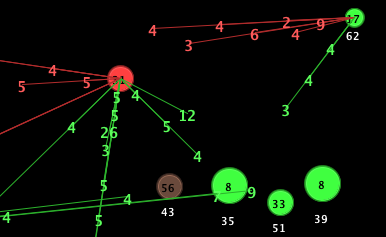
\includegraphics[scale=1]{modified_viz}
	\caption{Фрагмент модифицированного визуализатора}
	\label{fig:modif_viz}
\end{figure}
В частности: 
	\begin{myItemize}
	\item Была добавлена возможность менять скорость воспроизведения при помощи дополнительного аргумента во время вызова приложения. Изначально она была слишком медленной.
	\item Были добавлены линии, показывающие траекторию полёта флотилий. Часто было не понятно какая цифра куда движется.
	\item Была добавлена возможность передавать визуализатору дополнительную отладочную информацию касательно планет с последующим её выводом на экран (на рисунке белый цифры под планетами). Например при выборе цели для каждой планеты считается коэффициент, найти и сопоставить с конкретной планетой из логов было достаточно сложно.
	\end{myItemize}
\item[Написание тестов] \hfill \\ В подобной задаче безусловным подспорьем являются \emph{модульные тесты} (англ. ``\texttt{unit tests}''), которые также присутствуют в написанном ИИ
\item[Система игры на всех картах] \hfill \\
Для эффективной проверки производительности разрабатываемого ИИ был написан несложный \emph{сценарий} (англ. ``\texttt{script}'') для запуска бота на всех картах из начального набора. В конце работы он выдаёт статистическую информацию по тому сколько игр было выиграно, проиграно и за сколько ходов.
\end{description}



\subsection{Процесс разработки}
Процесс разработки бота можно разделить на несколько этапов:
\begin{myEnumerate}
\item Написание первого бота и тестирование его на всех картах против всех простых ботов, что идут в начальном наборе.
\item Улучшение бота до тех пора, пока он не будет побеждать в $100\%$ случаях.
\item ``Замораживание'' бота в его текущем состоянии и установка его на место противника и переход к пункту 2. Т.е. теперь задача играть против своего же бота, и улучшая следующее поколение прийти к полной победе над ним.
\item Периодически пользоваться TCP Server'ом (\url{http://www.benzedrine.cx/planetwars/}). Это неофициальный централизованный сервер, на котором можно в реальном времени сразиться с другими клиентами сервера. Главное отличие от официально сервера заключается в следующем:
	\begin{myEnumerate} 
	\item В скорости. Подключившись игра начинается практически сразу, в отличии от официального сервера, где каждый бот играет в среднем раз в пол часа.
	\item Не нужно заливать свой программный код на сервер. Код бота запускается на компьютере его владельца, тем самым давая возможность записывать логи для последующего анализа.
	\item Игроки на TCP Server'е зачастую очень сильные, по-этому для бота это всё равно что \emph{стресс тестирование}.
	\end{myEnumerate}
\item Если появляется ощущение, что бот уже достаточно работоспособный, его можно упаковывать и засылать на официальный сервер и переходить к пункту 3.
\end{myEnumerate}



\subsection{Выбор типа ИИ и метода его написания}
На рисунке \ref{fig:agent} (стр. \pageref{fig:agent}) показана модель простейшего агента. Если сравнить её с рисунком \ref{fig:pw_engine_process} (стр. \pageref{fig:pw_engine_process}), то можно заметить, что схема игрока №1 имеет те же составные  части (вход, выход, принятие решения), что и агент. По-этому автор считает уместным в данной задаче применение агентно-ореинтированного подхода. По сути надо реализовать белый ящик со знаком вопроса на рисунке \ref{fig:agent} или более формально функцию агента.

Характеристики игры очень похожи на свойства среды, в которых функционирует агент, играющий в шахматы за одним важным исключением. Средний \emph{коэффициент ветвления} в шахматах примерно равен 35. Т.е. в среднем на каждом полу-ходу игрок может выбирать среди 35 возможных решений, что даёт приблизительно $35^{100}$ различных комбинаций состояний игры. \citep{russell1995} При этом программа DeepBlue могла просмотреть только на 14 ходов вперёд. 

Изучая вопрос эффективности различных методов и подходов для написания ИИ, автор ознакомился с некоторыми мнениями специалистов. Так, Антон Сафонов (MSc, магистерская работа которого была посвящена комбинированию методов оптимизации роя частиц и монте-карло метода) считает, что данная задача должна решаться ``современными способами, т.е. необходимо сделать так, что бы не нужно было говорить программе как решать задачу, а что бы программа сама находила пути её решения''. Т.е. его идея заключалась в применении оптимизированных алгоритмов поиска, абстрагируясь от конкретных планет и флотилий до понятий вроде ``скопление сил'', решая тем самым проблему чрезмерного коэффициента ветвления в ВП. Автору такой подход, ввиду отсутствия необходимых познаний в данной области, показался слишком сложным и непонятным. Более того, ему кажется, что именно ``ручной'' способ написания ИИ в данном случае будет более эффективным.

Для написания агента с использованием конкретных правил и законов, а иначе говоря используя стратегию и тактику, необходимо использовать знания о том ``как работает мир''. Такой агент называется \emph{агентов основанным на модели}. \citep{russell1995} С учётом того, что автор не собирается использовать алгоритмов поиска, для просмотра всех вариантов развития событий, то для такого агента достаточно разработать систему рефлексов, т.е. механизмы реагирующие исключительно на текущее акты восприятия. Хотя некоторые аспекты алгоритма всё же можно рассматривать как предсказание, когда система защиты строится на предположении относительно некоторых планет (см. \ref{sec:selfdefense}).



\subsection{Характер среды}
``Критерии успеха, наряду с описанием среды, а также датчиков и исполнительных механизмов агента, предоставляют полную спецификацию задачи, с которой сталкивается агент'' \citep{russell1995} Критерием успеха или показателем производительности в случае игры ВП является счёт на конец соревнования в итоговой рейтинговой таблице, а так же результат каждой сыгранной партии. Во время локального тестирования на всех картах такими показателями являются также количество ходов, за которое бот победил и проиграл.

Существуют характеристики, по которым можно классифицировать среды в которых оперируют ИИ. \citep{russell1995} В данном случае имеет место форма взаимодействия ИИ-ов, представляющая собой детерминированную, поочередную, охватывающие двух игроков игру с \emph{нулевой суммой} и с \emph{полной информацией}. \citep{russell1995, morgenstern1947} Эти и другие свойства среды и их значения, применительно к данной игре приведены в таблице \ref{tab:evn_properties} (стр. \pageref{tab:evn_properties}).

\begin{table}[h!]
	\centering
	\begin{tabular}{ | p{3.6cm} | p{3cm} | p{7.2cm} |}	
	\hline
	Свойство среды & \raggedright Значение для среды & Почему? \\ \hline \hline
	\raggedright Наблюдаемая полностью или частично & \raggedright Полностью наблюдаемая & ИИ имеет доступ ко всем данным, необходимых для принятия решения. \\ \hline
	\raggedright Детерминированная, стохастическая или стратегическая & \raggedright Стратегическая &  Является таковой, если ``среда является детерминированной во всех отношениях, кроме действий других агентов''\citep{russell1995} \\ \hline
	\raggedright Эпизодическая или последовательная & \raggedright После\-до\-ва\-тель\-ная & Т.к. выбор игрока на каждом ходу влияет на все будущие решения \\ \hline
	\raggedright Статическая или динамическая & \raggedright Полуди\-на\-ми\-чес\-кая & Т.к. ``с течением времени сама среда не изменяется, а изменяются показатели производительности''. \citep{russell1995} Выбор принимается в условиях ограниченного времени. \\ \hline
	\raggedright Дискретная или непрерывная & \raggedright Дискретная & Т.к. игра ``имеет конечное количество различимых состояний'' и она ``связана с дискретным множеством восприятий и действий`` \citep{russell1995} \\ \hline
	\raggedright Одноагентная или мультиагентная & \raggedright Конкурентная мультиагентная среда & Т.к. имеет место соперничающая сущность Б, которая пытается максимизировать показатели своей производительности за счёт минимизации показателей сущности А \\ \hline
	\end{tabular}
	\caption{Характеристики среды игры ВП}
	\label{tab:evn_properties}
\end{table}



\section{Стратегия и тактика}
\label{sec:strategic}
В этом разделе описаны стратегии и тактики, которые автор применил и реализовал в своём агенте. Так же тут делается попытка связать их со знаниями о военном ремесле, описанными в трактате ``Искусство Войны'' (5-6 вв. до н. э.).

\begin{quote}
``Если используешь их[войска] в битве, но победа долго не приходит, их оружие притупляется, а рвение - ослабевает. Если осаждаешь города, их силы истощаются. Если подвергаешь войско длительной войне, запасов государства не хватит ... Поэтому я слышал об успехе быстрых военных походов, и не слышал об успехе затяжных.'' \citep{tzu1971art}
\end{quote}
Это правило действительно и тут, потому что игра продолжается максимум 200 ходов. Что бы достичь победы, медлить нельзя. В этой игре быстрота развёртывания сил и захвата планет очень важен. В момент главного сражения разница в одну планету может решить исход исход партии.

Как уже говорилось ранее в начале игры у обоих игроков условия совершенно идентичные. У каждого есть по планете с сотней кораблей, а все остальные планеты находятся на равных расстояниях от начальных планет игроков, т.к. карта симметричная. Из этого можно ещё раз подчеркнуть мысль, что исход каждого поединка зависит исключительно от алгоритмов игроков.

Общую стратегию, можно охарактеризовать как ``играть, что бы не проиграть'', т.к. по мнению автора главное в этой игре - правильная оборона, что будет раскрыто ниже (см. \ref{sec:selfdefense}).

Вся стратегия автора делиться на 6 этапов или элементов. Алгоритм проходит через все эти этапы принимает решение о выборе. Каждый из них описан далее более подробно.

\subsection{Первый ход и расширение}
Самым первым этапом игры является фаза ``развёртывания'', в которой особенно важно самый первый \emph{выбор}. Причина тому в симметричности первоначального состояния игры для обоих игроков. По-этому очень важно с первых секунд игры попытаться получить преимущество, выбрав планеты для первой атаки наиболее эффективно. 
\begin{quote}
``Тому, кто первым приходит на поле сражения и ожидает врага, будет
легко; тот, кто приходит после и должен спешить в бой, будет утомлен''  \\
\hfill \citep{tzu1971art}
\end{quote}

В отличае от шахмат в этой игре нету игрока идущего первым, оба игрока делаю свой первый полу-ход не зная о решении противника. Неправильное решение на первом шаге может закончиться быстрой победой противника. Пример на рисунке \ref{fig:first_move1}.

\begin{figure}[h]
	\centering
	%LaTeX with PSTricks extensions
%%Creator: inkscape 0.48.0
%%Please note this file requires PSTricks extensions
\psset{xunit=.5pt,yunit=.5pt,runit=.5pt}
\begin{pspicture}(416,277)
{
\newrgbcolor{curcolor}{0.60000002 0.60000002 0.60000002}
\pscustom[linewidth=8,linecolor=curcolor]
{
\newpath
\moveto(130.91307,99.4608)
\lineto(106.732834,100.90802)
}
}
{
\newrgbcolor{curcolor}{0.60000002 0.60000002 0.60000002}
\pscustom[linestyle=none,fillstyle=solid,fillcolor=curcolor]
{
\newpath
\moveto(107.522285,114.09828)
\lineto(70.492905,103.07703)
\lineto(105.943375,87.71776)
\closepath
}
}
{
\newrgbcolor{curcolor}{0.60000002 0.60000002 0.60000002}
\pscustom[linewidth=8,linecolor=curcolor]
{
\newpath
\moveto(107.522285,114.09828)
\lineto(70.492905,103.07703)
\lineto(105.943375,87.71776)
\closepath
}
}
{
\newrgbcolor{curcolor}{0 0 0}
\pscustom[linestyle=none,fillstyle=solid,fillcolor=curcolor]
{
\newpath
\moveto(86.845245,99.93384)
\lineto(88.313995,100.05884)
\curveto(88.42857833,99.34008667)(88.68378667,98.80102333)(89.07962,98.44165)
\curveto(89.47545333,98.08227667)(89.95462,97.90259)(90.51712,97.90259)
\curveto(91.19420333,97.90259)(91.76712,98.15779667)(92.23587,98.66821)
\curveto(92.70462,99.17863)(92.938995,99.85571333)(92.938995,100.69946)
\curveto(92.938995,101.50154667)(92.71503667,102.13436)(92.26712,102.5979)
\curveto(91.81920333,103.06144)(91.23066167,103.29321)(90.501495,103.29321)
\curveto(90.04316167,103.29321)(89.63170333,103.18904333)(89.26712,102.98071)
\curveto(88.90253667,102.77237667)(88.61607833,102.50675333)(88.407745,102.18384)
\lineto(87.095245,102.35571)
\lineto(88.20462,108.23071)
\lineto(93.89212,108.23071)
\lineto(93.89212,106.88696)
\lineto(89.32962,106.88696)
\lineto(88.70462,103.80884)
\curveto(89.39212,104.28800667)(90.11607833,104.52759)(90.876495,104.52759)
\curveto(91.876495,104.52759)(92.720245,104.18123667)(93.407745,103.48853)
\curveto(94.095245,102.79581667)(94.438995,101.90779333)(94.438995,100.82446)
\curveto(94.438995,99.78279333)(94.13691167,98.88696)(93.532745,98.13696)
\curveto(92.79316167,97.19946)(91.78795333,96.73071)(90.51712,96.73071)
\curveto(89.47545333,96.73071)(88.626495,97.02498333)(87.970245,97.61353)
\curveto(87.313995,98.20207)(86.938995,98.97550667)(86.845245,99.93384)
\closepath
\moveto(95.751495,102.59009)
\curveto(95.751495,103.94425667)(95.88951667,105.03279667)(96.16556,105.85571)
\curveto(96.4416,106.67863)(96.85566167,107.31404667)(97.407745,107.76196)
\curveto(97.95982833,108.20988)(98.65253667,108.43384)(99.48587,108.43384)
\curveto(100.10045333,108.43384)(100.63951667,108.31144333)(101.10306,108.06665)
\curveto(101.5666,107.82185667)(101.94941167,107.46508667)(102.251495,106.99634)
\curveto(102.55357833,106.52758667)(102.79055667,105.95987667)(102.96243,105.29321)
\curveto(103.13430667,104.62654333)(103.220245,103.72550333)(103.220245,102.59009)
\curveto(103.220245,101.24633667)(103.08222333,100.1604)(102.80618,99.33228)
\curveto(102.53014,98.50415333)(102.11607833,97.86352667)(101.563995,97.4104)
\curveto(101.01191167,96.95727333)(100.31920333,96.73071)(99.48587,96.73071)
\curveto(98.38170333,96.73071)(97.51191167,97.13175333)(96.876495,97.93384)
\curveto(96.126495,98.88175333)(95.751495,100.43383667)(95.751495,102.59009)
\closepath
\moveto(97.188995,102.59009)
\curveto(97.188995,100.70467)(97.41035,99.45206667)(97.85306,98.83228)
\curveto(98.29576667,98.21248667)(98.84003667,97.90259)(99.48587,97.90259)
\curveto(100.13170333,97.90259)(100.67337,98.21509)(101.11087,98.84009)
\curveto(101.54837,99.46509)(101.76712,100.71509)(101.76712,102.59009)
\curveto(101.76712,104.47550333)(101.54837,105.72810667)(101.11087,106.3479)
\curveto(100.67337,106.96769333)(100.126495,107.27759)(99.470245,107.27759)
\curveto(98.82441167,107.27759)(98.30878667,107.00154667)(97.92337,106.44946)
\curveto(97.43378667,105.75154667)(97.188995,104.46509)(97.188995,102.59009)
\closepath
}
}
{
\newrgbcolor{curcolor}{0.40000001 0.40000001 0.40000001}
\pscustom[linewidth=8,linecolor=curcolor]
{
\newpath
\moveto(285.3253,170.49428)
\lineto(303.0266,170.409424)
}
}
{
\newrgbcolor{curcolor}{0.40000001 0.40000001 0.40000001}
\pscustom[linestyle=none,fillstyle=solid,fillcolor=curcolor]
{
\newpath
\moveto(302.96326,157.19572)
\lineto(339.33096,170.23538)
\lineto(303.08997,183.62313)
\closepath
}
}
{
\newrgbcolor{curcolor}{0.40000001 0.40000001 0.40000001}
\pscustom[linewidth=8,linecolor=curcolor]
{
\newpath
\moveto(302.96326,157.19572)
\lineto(339.33096,170.23538)
\lineto(303.08997,183.62313)
\closepath
}
}
{
\newrgbcolor{curcolor}{1 1 1}
\pscustom[linestyle=none,fillstyle=solid,fillcolor=curcolor]
{
\newpath
\moveto(56.325462,24.61745)
\lineto(56.325462,24.61745)
\curveto(56.325462,35.94147)(65.413734,45.12138)(76.62468,45.12138)
\lineto(76.62468,45.12138)
\curveto(82.00836,45.12138)(87.17155,42.96117)(90.978386,39.11592)
\curveto(94.785225,35.27069)(96.92389,30.05544)(96.92389,24.61745)
\lineto(96.92389,24.61745)
\curveto(96.92389,13.29346)(87.835625,4.11353)(76.62468,4.11353)
\lineto(76.62468,4.11353)
\curveto(65.413734,4.11353)(56.325462,13.29346)(56.325462,24.61745)
\closepath
}
}
{
\newrgbcolor{curcolor}{0.02745098 0.21568628 0.3882353}
\pscustom[linewidth=2,linecolor=curcolor]
{
\newpath
\moveto(56.325462,24.61745)
\lineto(56.325462,24.61745)
\curveto(56.325462,35.94147)(65.413734,45.12138)(76.62468,45.12138)
\lineto(76.62468,45.12138)
\curveto(82.00836,45.12138)(87.17155,42.96117)(90.978386,39.11592)
\curveto(94.785225,35.27069)(96.92389,30.05544)(96.92389,24.61745)
\lineto(96.92389,24.61745)
\curveto(96.92389,13.29346)(87.835625,4.11353)(76.62468,4.11353)
\lineto(76.62468,4.11353)
\curveto(65.413734,4.11353)(56.325462,13.29346)(56.325462,24.61745)
\closepath
}
}
{
\newrgbcolor{curcolor}{1 1 1}
\pscustom[linestyle=none,fillstyle=solid,fillcolor=curcolor]
{
\newpath
\moveto(-4.304457,107.85104)
\lineto(-4.304457,107.85104)
\curveto(-4.304457,124.7066)(9.268013,138.37073)(26.010504,138.37073)
\lineto(26.010504,138.37073)
\curveto(34.05053,138.37073)(41.76126,135.15527)(47.44642,129.43173)
\curveto(53.131577,123.70818)(56.325462,115.94537)(56.325462,107.85104)
\lineto(56.325462,107.85104)
\curveto(56.325462,90.9955)(42.752995,77.33136)(26.010504,77.33136)
\lineto(26.010504,77.33136)
\curveto(9.268013,77.33136)(-4.304457,90.9955)(-4.304457,107.85104)
\closepath
}
}
{
\newrgbcolor{curcolor}{0.02745098 0.21568628 0.3882353}
\pscustom[linewidth=2,linecolor=curcolor]
{
\newpath
\moveto(-4.304457,107.85104)
\lineto(-4.304457,107.85104)
\curveto(-4.304457,124.7066)(9.268013,138.37073)(26.010504,138.37073)
\lineto(26.010504,138.37073)
\curveto(34.05053,138.37073)(41.76126,135.15527)(47.44642,129.43173)
\curveto(53.131577,123.70818)(56.325462,115.94537)(56.325462,107.85104)
\lineto(56.325462,107.85104)
\curveto(56.325462,90.9955)(42.752995,77.33136)(26.010504,77.33136)
\lineto(26.010504,77.33136)
\curveto(9.268013,77.33136)(-4.304457,90.9955)(-4.304457,107.85104)
\closepath
}
}
{
\newrgbcolor{curcolor}{1 1 1}
\pscustom[linestyle=none,fillstyle=solid,fillcolor=curcolor]
{
\newpath
\moveto(329.60373,252.866798)
\lineto(329.60373,252.866798)
\curveto(329.60373,241.542786)(320.51547,232.36286)(309.30453,232.36286)
\lineto(309.30453,232.36286)
\curveto(303.92084,232.36286)(298.75766,234.52309)(294.9508,238.368324)
\curveto(291.14398,242.21356)(289.0053,247.428816)(289.0053,252.866798)
\lineto(289.0053,252.866798)
\curveto(289.0053,264.190809)(298.09357,273.370735)(309.30453,273.370735)
\lineto(309.30453,273.370735)
\curveto(320.51547,273.370735)(329.60373,264.190809)(329.60373,252.866798)
\closepath
}
}
{
\newrgbcolor{curcolor}{0.02745098 0.21568628 0.3882353}
\pscustom[linewidth=2,linecolor=curcolor]
{
\newpath
\moveto(329.60373,252.866798)
\lineto(329.60373,252.866798)
\curveto(329.60373,241.542786)(320.51547,232.36286)(309.30453,232.36286)
\lineto(309.30453,232.36286)
\curveto(303.92084,232.36286)(298.75766,234.52309)(294.9508,238.368324)
\curveto(291.14398,242.21356)(289.0053,247.428816)(289.0053,252.866798)
\lineto(289.0053,252.866798)
\curveto(289.0053,264.190809)(298.09357,273.370735)(309.30453,273.370735)
\lineto(309.30453,273.370735)
\curveto(320.51547,273.370735)(329.60373,264.190809)(329.60373,252.866798)
\closepath
}
}
{
\newrgbcolor{curcolor}{1 1 1}
\pscustom[linestyle=none,fillstyle=solid,fillcolor=curcolor]
{
\newpath
\moveto(411.59848,168.89042)
\lineto(411.59848,168.89042)
\curveto(411.59848,152.03487)(398.02603,138.37073)(381.28354,138.37073)
\lineto(381.28354,138.37073)
\curveto(373.2435,138.37073)(365.53278,141.5862)(359.84763,147.30974)
\curveto(354.16245,153.033295)(350.96857,160.7961)(350.96857,168.89042)
\lineto(350.96857,168.89042)
\curveto(350.96857,185.74598)(364.54105,199.4101)(381.28354,199.4101)
\lineto(381.28354,199.4101)
\curveto(398.02603,199.4101)(411.59848,185.74598)(411.59848,168.89042)
\closepath
}
}
{
\newrgbcolor{curcolor}{0.02745098 0.21568628 0.3882353}
\pscustom[linewidth=2,linecolor=curcolor]
{
\newpath
\moveto(411.59848,168.89042)
\lineto(411.59848,168.89042)
\curveto(411.59848,152.03487)(398.02603,138.37073)(381.28354,138.37073)
\lineto(381.28354,138.37073)
\curveto(373.2435,138.37073)(365.53278,141.5862)(359.84763,147.30974)
\curveto(354.16245,153.033295)(350.96857,160.7961)(350.96857,168.89042)
\lineto(350.96857,168.89042)
\curveto(350.96857,185.74598)(364.54105,199.4101)(381.28354,199.4101)
\lineto(381.28354,199.4101)
\curveto(398.02603,199.4101)(411.59848,185.74598)(411.59848,168.89042)
\closepath
}
}
{
\newrgbcolor{curcolor}{0.60000002 0.60000002 0.60000002}
\pscustom[linewidth=8,linecolor=curcolor]
{
\newpath
\moveto(132.39711,69.30011)
\lineto(126.210434,64.17465)
}
}
{
\newrgbcolor{curcolor}{0.60000002 0.60000002 0.60000002}
\pscustom[linestyle=none,fillstyle=solid,fillcolor=curcolor]
{
\newpath
\moveto(117.78038,74.35013)
\lineto(98.25354,41.01328)
\lineto(134.64049,53.99918)
\closepath
}
}
{
\newrgbcolor{curcolor}{0.60000002 0.60000002 0.60000002}
\pscustom[linewidth=8,linecolor=curcolor]
{
\newpath
\moveto(117.78038,74.35013)
\lineto(98.25354,41.01328)
\lineto(134.64049,53.99918)
\closepath
}
}
{
\newrgbcolor{curcolor}{0 0 0}
\pscustom[linestyle=none,fillstyle=solid,fillcolor=curcolor]
{
\newpath
\moveto(116.54197,53.28534)
\lineto(116.54197,51.92596)
\lineto(108.963844,51.92596)
\curveto(108.953428,52.26971333)(109.01072,52.59784)(109.13572,52.91034)
\curveto(109.32322,53.42075333)(109.63051133,53.92596)(110.057594,54.42596)
\curveto(110.484678,54.92596)(111.09926133,55.50408667)(111.901344,56.16034)
\curveto(113.140928,57.18117333)(113.97947,57.99107)(114.41697,58.59003)
\curveto(114.85447,59.18898333)(115.07322,59.75408667)(115.07322,60.28534)
\curveto(115.07322,60.83742)(114.87530333,61.30617)(114.47947,61.69159)
\curveto(114.08363667,62.07700333)(113.56280333,62.26971)(112.91697,62.26971)
\curveto(112.239886,62.26971)(111.69821933,62.06658667)(111.29197,61.66034)
\curveto(110.88571933,61.25408667)(110.682594,60.69158667)(110.682594,59.97284)
\lineto(109.22947,60.11346)
\curveto(109.33363667,61.19679333)(109.70863667,62.01971)(110.35447,62.58221)
\curveto(111.00030333,63.14471)(111.86488667,63.42596)(112.94822,63.42596)
\curveto(114.05238667,63.42596)(114.92478333,63.12127333)(115.56541,62.5119)
\curveto(116.20603267,61.90252667)(116.526344,61.14992333)(116.526344,60.25409)
\curveto(116.526344,59.79575667)(116.432594,59.34523667)(116.245094,58.90253)
\curveto(116.057594,58.45981667)(115.745094,57.99367)(115.307594,57.50409)
\curveto(114.870094,57.01450333)(114.146136,56.34262667)(113.13572,55.48846)
\curveto(112.29196933,54.78012667)(111.75030267,54.29835667)(111.51072,54.04315)
\curveto(111.271136,53.78794333)(111.07321933,53.53534)(110.91697,53.28534)
\lineto(116.54197,53.28534)
\closepath
\moveto(118.057594,54.92596)
\lineto(119.526344,55.05096)
\curveto(119.640928,54.33221333)(119.89613667,53.79315333)(120.29197,53.43378)
\curveto(120.68780333,53.0744)(121.16697,52.89471)(121.72947,52.89471)
\curveto(122.40655267,52.89471)(122.97946933,53.14992)(123.44822,53.66034)
\curveto(123.91696933,54.17075333)(124.151344,54.84783667)(124.151344,55.69159)
\curveto(124.151344,56.49367)(123.927386,57.12648333)(123.47947,57.59003)
\curveto(123.03155267,58.05357)(122.44301067,58.28534)(121.713844,58.28534)
\curveto(121.25551067,58.28534)(120.84405267,58.18117333)(120.47947,57.97284)
\curveto(120.114886,57.76450667)(119.82842733,57.49888)(119.620094,57.17596)
\lineto(118.307594,57.34784)
\lineto(119.41697,63.22284)
\lineto(125.10447,63.22284)
\lineto(125.10447,61.87909)
\lineto(120.54197,61.87909)
\lineto(119.91697,58.80096)
\curveto(120.60447,59.28012667)(121.328428,59.51971)(122.088844,59.51971)
\curveto(123.088844,59.51971)(123.932594,59.17335667)(124.620094,58.48065)
\curveto(125.307594,57.78794333)(125.651344,56.89992333)(125.651344,55.81659)
\curveto(125.651344,54.77492333)(125.34926067,53.87909)(124.745094,53.12909)
\curveto(124.00551133,52.19159)(123.00030333,51.72284)(121.72947,51.72284)
\curveto(120.68780333,51.72284)(119.83884467,52.01711)(119.182594,52.60565)
\curveto(118.52634467,53.19419)(118.15134467,53.96762667)(118.057594,54.92596)
\closepath
}
}
{
\newrgbcolor{curcolor}{1 1 1}
\pscustom[linestyle=none,fillstyle=solid,fillcolor=curcolor]
{
\newpath
\moveto(312.9428,165.488464)
\lineto(312.9428,163.87909)
\lineto(303.95844,163.87909)
\curveto(303.94801333,164.28533933)(304.01051333,164.670756)(304.14594,165.03534)
\curveto(304.37511333,165.64992267)(304.7423,166.25408933)(305.2475,166.84784)
\curveto(305.7527,167.44158933)(306.47926667,168.12908933)(307.4272,168.91034)
\curveto(308.90636,170.11867333)(309.90636,171.07700667)(310.4272,171.78534)
\curveto(310.94802667,172.49367333)(311.20844,173.165548)(311.20844,173.800964)
\curveto(311.20844,174.45721467)(310.97146,175.01450667)(310.4975,175.47284)
\curveto(310.02354,175.93117333)(309.40635333,176.16034)(308.64594,176.16034)
\curveto(307.84384667,176.16034)(307.20061667,175.91815333)(306.71625,175.43378)
\curveto(306.23188333,174.94940267)(305.9897,174.28013067)(305.9897,173.425964)
\lineto(304.27094,173.59784)
\curveto(304.38551333,174.87908933)(304.82822,175.85565267)(305.59906,176.52753)
\curveto(306.36988667,177.19940333)(307.40113333,177.53534)(308.6928,177.53534)
\curveto(309.99489333,177.53534)(311.02614667,177.17336)(311.78656,176.4494)
\curveto(312.54698667,175.72544267)(312.9272,174.827006)(312.9272,173.75409)
\curveto(312.9272,173.21242333)(312.81521667,172.67857)(312.59125,172.15253)
\curveto(312.36728333,171.626486)(311.99749,171.07440267)(311.48187,170.49628)
\curveto(310.96625,169.91815333)(310.10948,169.11867333)(308.91156,168.09784)
\curveto(307.91156,167.25408933)(307.26833,166.683776)(306.98187,166.3869)
\curveto(306.69542333,166.09002667)(306.45844667,165.790548)(306.27094,165.488464)
\lineto(312.9428,165.488464)
\closepath
\moveto(314.53656,167.44159)
\lineto(316.3022,167.59784)
\curveto(316.4272,166.74367333)(316.72667333,166.10044333)(317.20062,165.66815)
\curveto(317.67458,165.23585933)(318.24489333,165.019714)(318.91156,165.019714)
\curveto(319.71365333,165.019714)(320.39334,165.32179733)(320.95062,165.925964)
\curveto(321.50791333,166.53013067)(321.78656,167.33742267)(321.78656,168.34784)
\curveto(321.78656,169.295756)(321.51833,170.045756)(320.98187,170.59784)
\curveto(320.44542333,171.14992267)(319.7449,171.425964)(318.8803,171.425964)
\curveto(318.34906,171.425964)(317.86729333,171.30356933)(317.435,171.05878)
\curveto(317.00270667,170.81398667)(316.66156,170.49367333)(316.41156,170.09784)
\lineto(314.83344,170.300964)
\lineto(316.16156,177.300964)
\lineto(322.9272,177.300964)
\lineto(322.9272,175.69159)
\lineto(317.4897,175.69159)
\lineto(316.7553,172.050964)
\curveto(317.57823333,172.613464)(318.43761333,172.894714)(319.33344,172.894714)
\curveto(320.52094667,172.894714)(321.52355,172.483256)(322.34125,171.66034)
\curveto(323.15895,170.83742267)(323.5678,169.78013067)(323.5678,168.488464)
\curveto(323.5678,167.25929733)(323.20843333,166.19679733)(322.4897,165.300964)
\curveto(321.6147,164.19679733)(320.42198667,163.644714)(318.91156,163.644714)
\curveto(317.67198667,163.644714)(316.66156667,163.99106933)(315.8803,164.68378)
\curveto(315.09906,165.37648667)(314.65114667,166.29575667)(314.53656,167.44159)
\closepath
}
}
{
\newrgbcolor{curcolor}{0.80000001 0.80000001 0.80000001}
\pscustom[linestyle=none,fillstyle=solid,fillcolor=curcolor]
{
\newpath
\moveto(123.30447,98.64174)
\lineto(123.30447,98.64174)
\curveto(123.30447,123.90767)(143.78656,144.38977)(169.0525,144.38977)
\lineto(169.0525,144.38977)
\curveto(181.18562,144.38977)(192.82182,139.5699)(201.40125,130.99048)
\curveto(209.98067,122.41106)(214.80054,110.77487)(214.80054,98.64174)
\lineto(214.80054,98.64174)
\curveto(214.80054,73.3758)(194.31844,52.8937)(169.0525,52.8937)
\lineto(169.0525,52.8937)
\curveto(143.78656,52.8937)(123.30447,73.3758)(123.30447,98.64174)
\closepath
}
}
{
\newrgbcolor{curcolor}{0.02745098 0.21568628 0.3882353}
\pscustom[linewidth=2,linecolor=curcolor]
{
\newpath
\moveto(123.30447,98.64174)
\lineto(123.30447,98.64174)
\curveto(123.30447,123.90767)(143.78656,144.38977)(169.0525,144.38977)
\lineto(169.0525,144.38977)
\curveto(181.18562,144.38977)(192.82182,139.5699)(201.40125,130.99048)
\curveto(209.98067,122.41106)(214.80054,110.77487)(214.80054,98.64174)
\lineto(214.80054,98.64174)
\curveto(214.80054,73.3758)(194.31844,52.8937)(169.0525,52.8937)
\lineto(169.0525,52.8937)
\curveto(143.78656,52.8937)(123.30447,73.3758)(123.30447,98.64174)
\closepath
}
}
{
\newrgbcolor{curcolor}{0.40000001 0.40000001 0.40000001}
\pscustom[linestyle=none,fillstyle=solid,fillcolor=curcolor]
{
\newpath
\moveto(295.27692,164.74803)
\lineto(295.27692,164.74803)
\curveto(295.27692,139.48209)(274.7948,119)(249.52887,119)
\lineto(249.52887,119)
\curveto(237.39574,119)(225.75955,123.81987)(217.18013,132.39929)
\curveto(208.60071,140.97871)(203.78084,152.6149)(203.78084,164.74803)
\lineto(203.78084,164.74803)
\curveto(203.78084,190.01397)(224.26292,210.49606)(249.52887,210.49606)
\lineto(249.52887,210.49606)
\curveto(274.7948,210.49606)(295.27692,190.01397)(295.27692,164.74803)
\closepath
}
}
{
\newrgbcolor{curcolor}{0.02745098 0.21568628 0.3882353}
\pscustom[linewidth=2,linecolor=curcolor]
{
\newpath
\moveto(295.27692,164.74803)
\lineto(295.27692,164.74803)
\curveto(295.27692,139.48209)(274.7948,119)(249.52887,119)
\lineto(249.52887,119)
\curveto(237.39574,119)(225.75955,123.81987)(217.18013,132.39929)
\curveto(208.60071,140.97871)(203.78084,152.6149)(203.78084,164.74803)
\lineto(203.78084,164.74803)
\curveto(203.78084,190.01397)(224.26292,210.49606)(249.52887,210.49606)
\lineto(249.52887,210.49606)
\curveto(274.7948,210.49606)(295.27692,190.01397)(295.27692,164.74803)
\closepath
}
}
{
\newrgbcolor{curcolor}{0 0 0}
\pscustom[linestyle=none,fillstyle=solid,fillcolor=curcolor]
{
\newpath
\moveto(168.23409,93.75505)
\lineto(168.23409,92.14568)
\lineto(159.24971,92.14568)
\curveto(159.23929667,92.55192667)(159.30179667,92.93734333)(159.43721,93.30193)
\curveto(159.66637667,93.91651)(160.03356333,94.52067667)(160.53877,95.11443)
\curveto(161.04398333,95.70817667)(161.77054667,96.39567667)(162.71846,97.17693)
\curveto(164.19762667,98.38526333)(165.19762667,99.34359667)(165.71846,100.05193)
\curveto(166.23929333,100.76026333)(166.49971,101.43213667)(166.49971,102.06755)
\curveto(166.49971,102.72380333)(166.26273,103.28109667)(165.78877,103.73943)
\curveto(165.31481667,104.19776333)(164.69763,104.42693)(163.93721,104.42693)
\curveto(163.13513,104.42693)(162.4919,104.18474)(162.00752,103.70036)
\curveto(161.52314667,103.21598667)(161.28096,102.54671667)(161.28096,101.69255)
\lineto(159.56221,101.86443)
\curveto(159.67679667,103.14567667)(160.11950667,104.12223667)(160.89034,104.79411)
\curveto(161.66117333,105.46599)(162.69242333,105.80193)(163.98409,105.80193)
\curveto(165.28617,105.80193)(166.31742,105.43995)(167.07784,104.71599)
\curveto(167.83825333,103.99203)(168.21846,103.09359333)(168.21846,102.02068)
\curveto(168.21846,101.47901333)(168.10648,100.94515667)(167.88252,100.41911)
\curveto(167.65856667,99.89307)(167.28877667,99.34098667)(166.77315,98.76286)
\curveto(166.25752333,98.18474)(165.40075333,97.38526333)(164.20284,96.36443)
\curveto(163.20284,95.52067667)(162.55961,94.95036333)(162.27315,94.65349)
\curveto(161.98669,94.35661667)(161.74971,94.05713667)(161.56221,93.75505)
\lineto(168.23409,93.75505)
\closepath
\moveto(169.82784,95.70818)
\lineto(171.59346,95.86443)
\curveto(171.71846,95.01026333)(172.01794,94.36703333)(172.4919,93.93474)
\curveto(172.96586,93.50244667)(173.53617333,93.2863)(174.20284,93.2863)
\curveto(175.00492,93.2863)(175.68460667,93.58838333)(176.2419,94.19255)
\curveto(176.79919333,94.79671667)(177.07784,95.60401)(177.07784,96.61443)
\curveto(177.07784,97.56234333)(176.80961,98.31234333)(176.27315,98.86443)
\curveto(175.73669,99.41651)(175.03617,99.69255)(174.17159,99.69255)
\curveto(173.64033667,99.69255)(173.15856333,99.57015333)(172.72627,99.32536)
\curveto(172.29398333,99.08057333)(171.95284,98.76026333)(171.70284,98.36443)
\lineto(170.12471,98.56755)
\lineto(171.45284,105.56755)
\lineto(178.21846,105.56755)
\lineto(178.21846,103.95818)
\lineto(172.78096,103.95818)
\lineto(172.04659,100.31755)
\curveto(172.86950333,100.88005)(173.72887667,101.1613)(174.62471,101.1613)
\curveto(175.81221,101.1613)(176.81481333,100.74984333)(177.63252,99.92693)
\curveto(178.45023333,99.10401)(178.85909,98.04671667)(178.85909,96.75505)
\curveto(178.85909,95.52588333)(178.49971333,94.46338333)(177.78096,93.56755)
\curveto(176.90596,92.46338333)(175.71325333,91.9113)(174.20284,91.9113)
\curveto(172.96325333,91.9113)(171.95283667,92.25765333)(171.17159,92.95036)
\curveto(170.39033667,93.64307333)(169.94242,94.56234667)(169.82784,95.70818)
\closepath
}
}
{
\newrgbcolor{curcolor}{1 1 1}
\pscustom[linestyle=none,fillstyle=solid,fillcolor=curcolor]
{
\newpath
\moveto(240.05421,170.06447)
\lineto(240.05421,171.67384)
\lineto(248.85109,171.67384)
\lineto(248.85109,170.37697)
\curveto(247.98650333,169.46030333)(247.12973333,168.23634333)(246.28078,166.70509)
\curveto(245.43182,165.17384333)(244.77296333,163.60092667)(244.30421,161.98634)
\curveto(243.97087667,160.85092667)(243.75733667,159.60613667)(243.66359,158.25197)
\lineto(241.94484,158.25197)
\curveto(241.96567333,159.32488333)(242.17661,160.61915333)(242.57765,162.13478)
\curveto(242.97869,163.65040667)(243.55681667,165.11134333)(244.31203,166.51759)
\curveto(245.06723667,167.92384333)(245.86671333,169.10613667)(246.71046,170.06447)
\lineto(240.05421,170.06447)
\closepath
\moveto(250.30421,161.81447)
\lineto(252.06984,161.97072)
\curveto(252.19484,161.11655333)(252.49432,160.47332333)(252.96828,160.04103)
\curveto(253.44223333,159.60873667)(254.01254333,159.39259)(254.67921,159.39259)
\curveto(255.48129667,159.39259)(256.16099333,159.69467333)(256.7183,160.29884)
\curveto(257.27558667,160.90300667)(257.55423,161.7103)(257.55423,162.72072)
\curveto(257.55423,163.66863333)(257.286,164.41863333)(256.74954,164.97072)
\curveto(256.21307333,165.5228)(255.51254667,165.79884)(254.64796,165.79884)
\curveto(254.11671333,165.79884)(253.63494333,165.67644533)(253.20265,165.431656)
\curveto(252.77035667,165.18686533)(252.42921,164.86655333)(252.17921,164.47072)
\lineto(250.60109,164.67384)
\lineto(251.92921,171.67384)
\lineto(258.69485,171.67384)
\lineto(258.69485,170.06447)
\lineto(253.25734,170.06447)
\lineto(252.52296,166.42384)
\curveto(253.34588,166.98634)(254.20525667,167.26759)(255.10109,167.26759)
\curveto(256.28859667,167.26759)(257.29120667,166.85613333)(258.10892,166.03322)
\curveto(258.92662667,165.2103)(259.33548,164.15300667)(259.33548,162.86134)
\curveto(259.33548,161.63217333)(258.97610333,160.56967333)(258.25735,159.67384)
\curveto(257.38235,158.56967333)(256.18963667,158.01759)(254.67921,158.01759)
\curveto(253.43963,158.01759)(252.42921333,158.36394533)(251.64796,159.056656)
\curveto(250.86671333,159.74936533)(250.41879667,160.66863667)(250.30421,161.81447)
\closepath
}
}
\end{pspicture}

	\caption{Ошибка первого игрока (светло-серый) на первом шаге}
	\label{fig:first_move1}
\end{figure}
В показанной ситуации начальные планеты игроков находятся очень близко друг от друга и один из участников не обращая на это внимание рассылает б\'{о}льшую часть своих кораблей на захват нейтральных. В то же время его противник не спешит распускать все корабли. В результате ошибки второй игрок следующим ходом захватит изначальную планету первого игрока и получи тем самым победное преимущество, т.к. начальные планеты имеют высокий коэффициент роста (обычно 5).

На самом деле при хорошей самообороне и правильно выбранной \emph{функции выбора цели} для атаки (см. \ref{sec:atack}) никакой особой логики в первый ход вкладывать не обязательно (будет видно далее). Хотя автор всё же разработал рефлекс\footnote{и назвал его ``блицкриг'', хотя название ``во-банк'' тут тоже подходит} который срабатывает на первом и последующих ходах, если ситуация такая как описана выше. Он оставляет все корабли на первом ходу, а на втором посылает все корабли на главную планету противника.

\subsection{Самооборона}
\label{sec:selfdefense}
Самооборону можно считать пожалуй самым важным этапом всей стратегии. От того как хорошо и безошибочно реализован этот модуль алгоритма зависит результативность всего бота. Побеждает тот, у кото суммарный прирост кораблей на всех планетах больше. По-этому потеря любой своей планеты ведёт к изменению этого отношения, а значит этого нельзя допустить ни в кое случае.
\begin{quote}
``Поэтому тот, кто преуспел в войне, первым делом выбирает позицию, где он не может быть разбит, вместе с тем не упуская [любой возможности] разбить врага.'' \\
\citep{tzu1971art}
\end{quote}

Суть самообороны в том, что бы на планете всегда оставалось достаточно кораблей, что бы смочь отбить любую атаку. Для этого прежде всего надо посмотреть сколько и какие флотилии летят на данный момент на планету и представив, что более никакая планета не выпустит флотилий по данному направлению, просиммировать все прилёты кораблей получив в результате чёткое представление о судьбе этой планеты. 

Для удобства была написана специальная функция, которая занимается симуляцией таких случаев. В результате она выдаёт информацию о том на каких ходах и как будет меняться состояние этой планеты (количество кораблей, принадлежность) по мере прилёта флотилий. Из этой информации можно сделать определённый и важный вывод - сколько кораблей необходимо забронировать на самооборону, что бы когда прилетит последняя флотилия планета осталась у игрока.

На рисунке \ref{fig:simulation} упрощенно объясняется как работает алгоритм симуляции. 

\begin{figure}[h]
	\centering
	%LaTeX with PSTricks extensions
%%Creator: inkscape 0.48.0
%%Please note this file requires PSTricks extensions
\psset{xunit=.5pt,yunit=.5pt,runit=.5pt}
\begin{pspicture}(851,346)
{
\newrgbcolor{curcolor}{0.91764706 0.60000002 0.60000002}
\pscustom[linestyle=none,fillstyle=solid,fillcolor=curcolor]
{
\newpath
\moveto(623.1837,98.55011)
\lineto(623.1837,98.55011)
\curveto(623.1837,101.29855)(625.41174,103.5266)(628.1602,103.5266)
\lineto(648.097,103.5266)
\lineto(648.097,103.5266)
\curveto(649.4169,103.5266)(650.6826,103.00229)(651.6159,102.06902)
\curveto(652.5492,101.13574)(653.0735,99.86996)(653.0735,98.55011)
\lineto(653.0735,78.6448)
\curveto(653.0735,75.89636)(650.84546,73.66833)(648.097,73.66833)
\lineto(628.1602,73.66833)
\curveto(625.41174,73.66833)(623.1837,75.89636)(623.1837,78.6448)
\closepath
}
}
{
\newrgbcolor{curcolor}{0.60000002 0.60000002 0.60000002}
\pscustom[linewidth=2,linecolor=curcolor]
{
\newpath
\moveto(623.1837,98.55011)
\lineto(623.1837,98.55011)
\curveto(623.1837,101.29855)(625.41174,103.5266)(628.1602,103.5266)
\lineto(648.097,103.5266)
\lineto(648.097,103.5266)
\curveto(649.4169,103.5266)(650.6826,103.00229)(651.6159,102.06902)
\curveto(652.5492,101.13574)(653.0735,99.86996)(653.0735,98.55011)
\lineto(653.0735,78.6448)
\curveto(653.0735,75.89636)(650.84546,73.66833)(648.097,73.66833)
\lineto(628.1602,73.66833)
\curveto(625.41174,73.66833)(623.1837,75.89636)(623.1837,78.6448)
\closepath
}
}
{
\newrgbcolor{curcolor}{0.02745098 0.21568628 0.3882353}
\pscustom[linewidth=2,linecolor=curcolor]
{
\newpath
\moveto(51.388927,275.692566)
\lineto(722.0346,275.692566)
}
}
{
\newrgbcolor{curcolor}{0.02745098 0.21568628 0.3882353}
\pscustom[linestyle=none,fillstyle=solid,fillcolor=curcolor]
{
\newpath
\moveto(722.0346,272.3891)
\lineto(731.1108,275.692566)
\lineto(722.0346,278.99603)
\closepath
}
}
{
\newrgbcolor{curcolor}{0.02745098 0.21568628 0.3882353}
\pscustom[linewidth=2,linecolor=curcolor]
{
\newpath
\moveto(722.0346,272.3891)
\lineto(731.1108,275.692566)
\lineto(722.0346,278.99603)
\closepath
}
}
{
\newrgbcolor{curcolor}{0.02745098 0.21568628 0.3882353}
\pscustom[linewidth=2,linecolor=curcolor]
{
\newpath
\moveto(52.582676,289.94882)
\lineto(52.582676,259.93307)
}
}
{
\newrgbcolor{curcolor}{0 0 0}
\pscustom[linestyle=none,fillstyle=solid,fillcolor=curcolor]
{
\newpath
\moveto(19.817053,325.887138)
\lineto(19.817053,337.887139)
\lineto(15.348302,337.887139)
\lineto(15.348302,339.4808893)
\lineto(26.113928,339.4808893)
\lineto(26.113928,337.887139)
\lineto(21.613928,337.887139)
\lineto(21.613928,325.887138)
\lineto(19.817053,325.887138)
\closepath
\moveto(34.2858,329.059013)
\lineto(36.00455,328.840263)
\curveto(35.73371667,327.840263)(35.23111333,327.06161733)(34.49674,326.504326)
\curveto(33.762364,325.947034)(32.82226,325.668388)(31.676428,325.668388)
\curveto(30.238928,325.668388)(29.098303,326.11109633)(28.254553,326.996513)
\curveto(27.410803,327.88192967)(26.988928,329.12672167)(26.988928,330.730889)
\curveto(26.988928,332.387139)(27.413407,333.67359733)(28.262365,334.590264)
\curveto(29.11132367,335.50693067)(30.21809467,335.965264)(31.582678,335.965264)
\curveto(32.90559267,335.965264)(33.98371667,335.51734733)(34.81705,334.621514)
\curveto(35.65038333,333.72568067)(36.06705,332.46005567)(36.06705,330.824639)
\curveto(36.06705,330.730889)(36.061842,330.58505567)(36.051426,330.387139)
\lineto(28.707678,330.387139)
\curveto(28.770178,329.303805)(29.07746967,328.47567967)(29.629553,327.902763)
\curveto(30.18163633,327.32984633)(30.86913633,327.043388)(31.692053,327.043388)
\curveto(32.29621767,327.043388)(32.81444667,327.202242)(33.24674,327.51995)
\curveto(33.67903067,327.83765867)(34.025384,328.35067967)(34.2858,329.059013)
\closepath
\moveto(28.801428,331.762139)
\lineto(34.301426,331.762139)
\curveto(34.22850867,332.58505567)(34.02017533,333.20484733)(33.676426,333.621514)
\curveto(33.14517533,334.26734733)(32.45246767,334.590264)(31.598303,334.590264)
\curveto(30.83788633,334.590264)(30.194657,334.33245167)(29.668615,333.816827)
\curveto(29.14257367,333.30120167)(28.85351133,332.61630567)(28.801428,331.762139)
\closepath
\moveto(37.9108,335.746514)
\lineto(39.56705,335.746514)
\lineto(39.56705,331.480889)
\curveto(40.10871667,331.480889)(40.48371667,331.58245167)(40.69205,331.785577)
\curveto(40.90038333,331.98870167)(41.21288333,332.58505567)(41.62955,333.574639)
\curveto(41.96288333,334.34547233)(42.23111333,334.855889)(42.43424,335.105889)
\curveto(42.637364,335.355889)(42.87173833,335.52516)(43.137363,335.613702)
\curveto(43.40298767,335.70224333)(43.82746667,335.746514)(44.4108,335.746514)
\lineto(44.75455,335.746514)
\lineto(44.75455,334.355889)
\lineto(44.2858,334.371514)
\curveto(43.8483,334.371514)(43.56705,334.30380567)(43.44205,334.168389)
\curveto(43.31705,334.03297233)(43.11913333,333.62672233)(42.8483,332.949639)
\curveto(42.5983,332.31422233)(42.36653,331.871514)(42.15299,331.621514)
\curveto(41.93944733,331.371514)(41.613926,331.14755567)(41.176426,330.949639)
\curveto(41.89517533,330.75172233)(42.60350867,330.079847)(43.301426,328.934013)
\lineto(45.12955,325.887138)
\lineto(43.2858,325.887138)
\lineto(41.50455,328.934013)
\curveto(41.13996733,329.54859633)(40.82225933,329.95484667)(40.551426,330.152764)
\curveto(40.28059267,330.35068067)(39.95246733,330.449639)(39.56705,330.449639)
\lineto(39.56705,325.887138)
\lineto(37.9108,325.887138)
\lineto(37.9108,335.746514)
\closepath
\moveto(46.00455,322.090263)
\lineto(45.832676,323.652763)
\curveto(46.19725867,323.559013)(46.51496667,323.512138)(46.7858,323.512138)
\curveto(47.150384,323.512138)(47.444655,323.574638)(47.668613,323.699638)
\curveto(47.892571,323.824638)(48.07746667,323.996513)(48.2233,324.215263)
\curveto(48.32746667,324.38192967)(48.49413333,324.79859633)(48.7233,325.465263)
\curveto(48.75455067,325.559013)(48.806634,325.69442967)(48.87955,325.871513)
\lineto(45.145176,335.746514)
\lineto(46.94205,335.746514)
\lineto(48.988926,330.027764)
\curveto(49.25975933,329.30901333)(49.49934267,328.54859633)(49.707676,327.746513)
\curveto(49.895176,328.51734633)(50.12434267,329.26734633)(50.395176,329.996513)
\lineto(52.488926,335.746514)
\lineto(54.1608,335.746514)
\lineto(50.4108,325.715263)
\curveto(50.01496667,324.63192967)(49.70246667,323.887138)(49.4733,323.480888)
\curveto(49.18163333,322.92880467)(48.843092,322.52515867)(48.457676,322.26995)
\curveto(48.07225867,322.014742)(47.61392533,321.887138)(47.082676,321.887138)
\curveto(46.75975867,321.887138)(46.40038333,321.95484633)(46.00455,322.090263)
\closepath
\moveto(55.4733,335.746514)
\lineto(57.145176,335.746514)
\lineto(57.145176,327.262138)
\lineto(60.94205,327.262138)
\lineto(60.94205,335.746514)
\lineto(62.613926,335.746514)
\lineto(62.613926,327.262138)
\lineto(66.42643,327.262138)
\lineto(66.42643,335.746514)
\lineto(68.08268,335.746514)
\lineto(68.08268,327.262138)
\lineto(69.192055,327.262138)
\lineto(69.192055,323.090263)
\lineto(67.80143,323.090263)
\lineto(67.80143,325.887138)
\lineto(55.4733,325.887138)
\lineto(55.4733,335.746514)
\closepath
\moveto(77.504555,329.059013)
\lineto(79.223305,328.840263)
\curveto(78.95247167,327.840263)(78.44986667,327.06161733)(77.71549,326.504326)
\curveto(76.98111667,325.947034)(76.04101333,325.668388)(74.89518,325.668388)
\curveto(73.45768,325.668388)(72.317055,326.11109633)(71.473305,326.996513)
\curveto(70.629555,327.88192967)(70.20768,329.12672167)(70.20768,330.730889)
\curveto(70.20768,332.387139)(70.63216,333.67359733)(71.48112,334.590264)
\curveto(72.33007667,335.50693067)(73.43684667,335.965264)(74.80143,335.965264)
\curveto(76.12434667,335.965264)(77.20247167,335.51734733)(78.035805,334.621514)
\curveto(78.86913833,333.72568067)(79.285805,332.46005567)(79.285805,330.824639)
\curveto(79.285805,330.730889)(79.28059667,330.58505567)(79.27018,330.387139)
\lineto(71.92643,330.387139)
\curveto(71.98893,329.303805)(72.29622167,328.47567967)(72.848305,327.902763)
\curveto(73.40038833,327.32984633)(74.08788833,327.043388)(74.910805,327.043388)
\curveto(75.51497167,327.043388)(76.0332,327.202242)(76.46549,327.51995)
\curveto(76.89778333,327.83765867)(77.24413833,328.35067967)(77.504555,329.059013)
\closepath
\moveto(72.02018,331.762139)
\lineto(77.52018,331.762139)
\curveto(77.44726333,332.58505567)(77.23893,333.20484733)(76.89518,333.621514)
\curveto(76.36393,334.26734733)(75.67122167,334.590264)(74.817055,334.590264)
\curveto(74.05663833,334.590264)(73.41341,334.33245167)(72.88737,333.816827)
\curveto(72.36132667,333.30120167)(72.07226333,332.61630567)(72.02018,331.762139)
\closepath
\moveto(87.879555,329.059013)
\lineto(89.598305,328.840263)
\curveto(89.32747167,327.840263)(88.82486667,327.06161733)(88.09049,326.504326)
\curveto(87.35611667,325.947034)(86.41601333,325.668388)(85.27018,325.668388)
\curveto(83.83268,325.668388)(82.692055,326.11109633)(81.848305,326.996513)
\curveto(81.004555,327.88192967)(80.58268,329.12672167)(80.58268,330.730889)
\curveto(80.58268,332.387139)(81.00716,333.67359733)(81.85612,334.590264)
\curveto(82.70507667,335.50693067)(83.81184667,335.965264)(85.17643,335.965264)
\curveto(86.49934667,335.965264)(87.57747167,335.51734733)(88.410805,334.621514)
\curveto(89.24413833,333.72568067)(89.660805,332.46005567)(89.660805,330.824639)
\curveto(89.660805,330.730889)(89.65559667,330.58505567)(89.64518,330.387139)
\lineto(82.30143,330.387139)
\curveto(82.36393,329.303805)(82.67122167,328.47567967)(83.223305,327.902763)
\curveto(83.77538833,327.32984633)(84.46288833,327.043388)(85.285805,327.043388)
\curveto(85.88997167,327.043388)(86.4082,327.202242)(86.84049,327.51995)
\curveto(87.27278333,327.83765867)(87.61913833,328.35067967)(87.879555,329.059013)
\closepath
\moveto(82.39518,331.762139)
\lineto(87.89518,331.762139)
\curveto(87.82226333,332.58505567)(87.61393,333.20484733)(87.27018,333.621514)
\curveto(86.73893,334.26734733)(86.04622167,334.590264)(85.192055,334.590264)
\curveto(84.43163833,334.590264)(83.78841,334.33245167)(83.26237,333.816827)
\curveto(82.73632667,333.30120167)(82.44726333,332.61630567)(82.39518,331.762139)
\closepath
}
}
{
\newrgbcolor{curcolor}{0 0 0}
\pscustom[linestyle=none,fillstyle=solid,fillcolor=curcolor]
{
\newpath
\moveto(15.692052,308.496513)
\lineto(17.332678,308.277763)
\curveto(17.15559467,307.152763)(16.697261,306.26995067)(15.957677,305.629326)
\curveto(15.21809367,304.988702)(14.30663533,304.66839)(13.223302,304.66839)
\curveto(11.879552,304.66839)(10.79882267,305.10849333)(9.981114,305.9887)
\curveto(9.163406,306.86890867)(8.754552,308.13192967)(8.754552,309.777763)
\curveto(8.754552,310.840263)(8.929031,311.76995067)(9.277989,312.566826)
\curveto(9.62694767,313.363702)(10.163406,313.96266)(10.887364,314.3637)
\curveto(11.61132267,314.764742)(12.395177,314.965263)(13.238927,314.965263)
\curveto(14.31184367,314.965263)(15.18684367,314.69442967)(15.863927,314.152763)
\curveto(16.541011,313.61109633)(16.97851133,312.840263)(17.176428,311.840263)
\lineto(15.551427,311.590263)
\curveto(15.395177,312.25692967)(15.11913533,312.75692967)(14.723302,313.090263)
\curveto(14.32746867,313.42359633)(13.85351033,313.590263)(13.301427,313.590263)
\curveto(12.457677,313.590263)(11.772781,313.28817967)(11.246739,312.684013)
\curveto(10.72069767,312.07984633)(10.457677,311.126722)(10.457677,309.82464)
\curveto(10.457677,308.501722)(10.71288533,307.540784)(11.223302,306.941826)
\curveto(11.73371867,306.34286867)(12.395177,306.04339)(13.207677,306.04339)
\curveto(13.863927,306.04339)(14.410802,306.24391)(14.848302,306.64495)
\curveto(15.285802,307.045992)(15.567052,307.66317967)(15.692052,308.496513)
\closepath
\moveto(17.957678,309.809013)
\curveto(17.957678,311.631931)(18.46809467,312.98609767)(19.488928,313.871513)
\curveto(20.332678,314.60067967)(21.363928,314.965263)(22.582678,314.965263)
\curveto(23.93684467,314.965263)(25.04361533,314.51995067)(25.90299,313.629326)
\curveto(26.76236533,312.738702)(27.192053,311.51214)(27.192053,309.94964)
\curveto(27.192053,308.67880667)(27.00194867,307.68141)(26.62174,306.95745)
\curveto(26.241532,306.233492)(25.68944867,305.670992)(24.96549,305.26995)
\curveto(24.241532,304.86891)(23.44726133,304.66839)(22.582678,304.66839)
\curveto(21.207678,304.66839)(20.09309467,305.11109767)(19.238928,305.996513)
\curveto(18.38476133,306.881931)(17.957678,308.15276433)(17.957678,309.809013)
\closepath
\moveto(19.676428,309.809013)
\curveto(19.676428,308.54859767)(19.95246967,307.60589)(20.504553,306.98089)
\curveto(21.05663633,306.35589)(21.74934467,306.04339)(22.582678,306.04339)
\curveto(23.41601133,306.04339)(24.10611533,306.35849333)(24.65299,306.9887)
\curveto(25.19986533,307.61890867)(25.473303,308.57984633)(25.473303,309.871513)
\curveto(25.473303,311.09026433)(25.19726133,312.01214)(24.645178,312.63714)
\curveto(24.09309467,313.26214)(23.40559467,313.57464)(22.582678,313.57464)
\curveto(21.74934467,313.57464)(21.05663633,313.26214)(20.504553,312.63714)
\curveto(19.95246967,312.01214)(19.676428,311.069431)(19.676428,309.809013)
\closepath
\moveto(35.395176,308.496513)
\lineto(37.0358,308.277763)
\curveto(36.85871733,307.152763)(36.400384,306.26995067)(35.6608,305.629326)
\curveto(34.92121733,304.988702)(34.00975933,304.66839)(32.926426,304.66839)
\curveto(31.58267733,304.66839)(30.50194867,305.10849333)(29.68424,305.9887)
\curveto(28.866532,306.86890867)(28.457678,308.13192967)(28.457678,309.777763)
\curveto(28.457678,310.840263)(28.632157,311.76995067)(28.981115,312.566826)
\curveto(29.33007367,313.363702)(29.866532,313.96266)(30.59049,314.3637)
\curveto(31.31444867,314.764742)(32.098302,314.965263)(32.94205,314.965263)
\curveto(34.01496733,314.965263)(34.88996733,314.69442967)(35.56705,314.152763)
\curveto(36.244134,313.61109633)(36.681634,312.840263)(36.87955,311.840263)
\lineto(35.25455,311.590263)
\curveto(35.09830067,312.25692967)(34.82225933,312.75692967)(34.426426,313.090263)
\curveto(34.03059267,313.42359633)(33.556634,313.590263)(33.00455,313.590263)
\curveto(32.160802,313.590263)(31.475907,313.28817967)(30.949865,312.684013)
\curveto(30.42382367,312.07984633)(30.160803,311.126722)(30.160803,309.82464)
\curveto(30.160803,308.501722)(30.41601133,307.540784)(30.926428,306.941826)
\curveto(31.43684467,306.34286867)(32.098302,306.04339)(32.9108,306.04339)
\curveto(33.56705067,306.04339)(34.113926,306.24391)(34.551426,306.64495)
\curveto(34.988926,307.045992)(35.270176,307.66317967)(35.395176,308.496513)
\closepath
\moveto(37.395176,314.746513)
\lineto(45.395176,314.746513)
\lineto(45.395176,313.35589)
\lineto(42.2233,313.35589)
\lineto(42.2233,304.88714)
\lineto(40.56705,304.88714)
\lineto(40.56705,313.35589)
\lineto(37.395176,313.35589)
\lineto(37.395176,314.746513)
\closepath
\moveto(46.19205,309.809013)
\curveto(46.19205,311.631931)(46.70246667,312.98609767)(47.7233,313.871513)
\curveto(48.56705067,314.60067967)(49.59830067,314.965263)(50.81705,314.965263)
\curveto(52.17121667,314.965263)(53.27798767,314.51995067)(54.137363,313.629326)
\curveto(54.99673833,312.738702)(55.426426,311.51214)(55.426426,309.94964)
\curveto(55.426426,308.67880667)(55.23632167,307.68141)(54.856113,306.95745)
\curveto(54.47590433,306.233492)(53.923821,305.670992)(53.199863,305.26995)
\curveto(52.475905,304.86891)(51.681634,304.66839)(50.81705,304.66839)
\curveto(49.44205,304.66839)(48.32746667,305.11109767)(47.4733,305.996513)
\curveto(46.61913333,306.881931)(46.19205,308.15276433)(46.19205,309.809013)
\closepath
\moveto(47.9108,309.809013)
\curveto(47.9108,308.54859767)(48.186842,307.60589)(48.738926,306.98089)
\curveto(49.29100867,306.35589)(49.98371667,306.04339)(50.81705,306.04339)
\curveto(51.65038333,306.04339)(52.34048767,306.35849333)(52.887363,306.9887)
\curveto(53.43423833,307.61890867)(53.707676,308.57984633)(53.707676,309.871513)
\curveto(53.707676,311.09026433)(53.431634,312.01214)(52.87955,312.63714)
\curveto(52.32746733,313.26214)(51.63996733,313.57464)(50.81705,313.57464)
\curveto(49.98371667,313.57464)(49.29100867,313.26214)(48.738926,312.63714)
\curveto(48.186842,312.01214)(47.9108,311.069431)(47.9108,309.809013)
\closepath
\moveto(64.973305,314.746513)
\lineto(64.973305,304.88714)
\lineto(63.301426,304.88714)
\lineto(63.301426,308.73089)
\lineto(62.3483,308.73089)
\curveto(61.75455067,308.73089)(61.31444733,308.65536867)(61.02799,308.504326)
\curveto(60.74153,308.353284)(60.32225867,307.86630533)(59.770176,307.04339)
\lineto(58.31705,304.88714)
\lineto(56.238926,304.88714)
\lineto(58.051426,307.54339)
\curveto(58.59309267,308.35589)(59.13996733,308.81422333)(59.69205,308.91839)
\curveto(58.73371667,309.04339)(58.02538333,309.38453533)(57.56705,309.941826)
\curveto(57.10871667,310.49911733)(56.87955,311.14234633)(56.87955,311.871513)
\curveto(56.87955,312.71526433)(57.18163333,313.40536867)(57.7858,313.941826)
\curveto(58.38996667,314.478284)(59.25975867,314.746513)(60.395176,314.746513)
\lineto(64.973305,314.746513)
\closepath
\moveto(63.301426,313.35589)
\lineto(60.926426,313.35589)
\curveto(59.936842,313.35589)(59.29621667,313.20224333)(59.00455,312.89495)
\curveto(58.71288333,312.58765867)(58.56705,312.22567967)(58.56705,311.809013)
\curveto(58.56705,311.22567967)(58.780592,310.795992)(59.207676,310.51995)
\curveto(59.63475867,310.24391)(60.38475867,310.10589)(61.457676,310.10589)
\lineto(63.301426,310.10589)
\lineto(63.301426,313.35589)
\closepath
\moveto(67.317055,314.746513)
\lineto(68.98893,314.746513)
\lineto(68.98893,310.63714)
\lineto(73.61393,310.63714)
\lineto(73.61393,314.746513)
\lineto(75.285805,314.746513)
\lineto(75.285805,304.88714)
\lineto(73.61393,304.88714)
\lineto(73.61393,309.26214)
\lineto(68.98893,309.26214)
\lineto(68.98893,304.88714)
\lineto(67.317055,304.88714)
\lineto(67.317055,314.746513)
\closepath
\moveto(77.598305,314.746513)
\lineto(79.27018,314.746513)
\lineto(79.27018,307.23089)
\lineto(83.89518,314.746513)
\lineto(85.70768,314.746513)
\lineto(85.70768,304.88714)
\lineto(84.035805,304.88714)
\lineto(84.035805,312.35589)
\lineto(79.39518,304.88714)
\lineto(77.598305,304.88714)
\lineto(77.598305,314.746513)
\closepath
\moveto(94.77018,308.059013)
\lineto(96.48893,307.840263)
\curveto(96.21809667,306.840263)(95.71549333,306.06161733)(94.98112,305.504326)
\curveto(94.24674333,304.94703533)(93.30663833,304.66839)(92.160805,304.66839)
\curveto(90.723305,304.66839)(89.58268,305.11109767)(88.73893,305.996513)
\curveto(87.89518,306.881931)(87.473305,308.12672333)(87.473305,309.73089)
\curveto(87.473305,311.38713867)(87.89778333,312.67359633)(88.74674,313.590263)
\curveto(89.5957,314.50692967)(90.70247167,314.965263)(92.067055,314.965263)
\curveto(93.38997167,314.965263)(94.46809667,314.51734633)(95.30143,313.621513)
\curveto(96.13476333,312.72567967)(96.55143,311.46005533)(96.55143,309.82464)
\curveto(96.55143,309.73088867)(96.54622167,309.58505533)(96.535805,309.38714)
\lineto(89.192055,309.38714)
\curveto(89.254555,308.30380667)(89.56184667,307.475681)(90.11393,306.902763)
\curveto(90.66601333,306.32984767)(91.35351333,306.04339)(92.17643,306.04339)
\curveto(92.78059667,306.04339)(93.29882667,306.20224333)(93.73112,306.51995)
\curveto(94.16341,306.83765867)(94.50976333,307.35067967)(94.77018,308.059013)
\closepath
\moveto(89.285805,310.76214)
\lineto(94.785805,310.76214)
\curveto(94.71288833,311.58505533)(94.504555,312.20484633)(94.160805,312.621513)
\curveto(93.629555,313.26734633)(92.93684667,313.590263)(92.08268,313.590263)
\curveto(91.32226333,313.590263)(90.67903333,313.33245067)(90.15299,312.816826)
\curveto(89.62695,312.301202)(89.33788833,311.61630667)(89.285805,310.76214)
\closepath
}
}
{
\newrgbcolor{curcolor}{0 0 0}
\pscustom[linestyle=none,fillstyle=solid,fillcolor=curcolor]
{
\newpath
\moveto(683.6613,243.091866)
\lineto(683.6613,256.685616)
\lineto(688.7707,256.685616)
\curveto(689.80194667,256.685616)(690.63268,256.55019933)(691.2629,256.279366)
\curveto(691.8931,256.00853267)(692.38528,255.58665733)(692.73944,255.01374)
\curveto(693.09361333,254.440824)(693.2707,253.841866)(693.2707,253.216866)
\curveto(693.2707,252.63353267)(693.11444667,252.084054)(692.80194,251.56843)
\curveto(692.48944667,251.05280333)(692.01028,250.63874)(691.36444,250.32624)
\curveto(692.18734667,250.08665733)(692.82016667,249.67519933)(693.2629,249.091866)
\curveto(693.70559333,248.50853267)(693.92694,247.82103267)(693.92694,247.029366)
\curveto(693.92694,246.39394867)(693.79412667,245.80280333)(693.5285,245.25593)
\curveto(693.26288,244.709054)(692.93214667,244.28717733)(692.5363,243.9903)
\curveto(692.14048,243.69342667)(691.64308,243.46947)(691.0441,243.31843)
\curveto(690.44516667,243.16738733)(689.7134,243.091866)(688.8488,243.091866)
\lineto(683.6613,243.091866)
\closepath
\moveto(685.4582,250.98249)
\lineto(688.3957,250.98249)
\curveto(689.19776667,250.98249)(689.77068,251.03457333)(690.11444,251.13874)
\curveto(690.57277333,251.27415733)(690.91912667,251.498116)(691.1535,251.810616)
\curveto(691.38788,252.123116)(691.50507,252.51894933)(691.50507,252.998116)
\curveto(691.50507,253.446032)(691.39569333,253.84186533)(691.17694,254.185616)
\curveto(690.95818,254.52936533)(690.64828333,254.76634333)(690.24725,254.89655)
\curveto(689.84621667,255.02676067)(689.15611333,255.091866)(688.17694,255.091866)
\lineto(685.4582,255.091866)
\lineto(685.4582,250.98249)
\closepath
\moveto(685.4582,244.70124)
\lineto(688.8488,244.70124)
\curveto(689.43213333,244.70124)(689.83839,244.72207333)(690.06757,244.76374)
\curveto(690.48423667,244.83665733)(690.83319333,244.959054)(691.11444,245.13093)
\curveto(691.39568,245.30280333)(691.62484667,245.55540667)(691.80194,245.88874)
\curveto(691.97902667,246.22207333)(692.06757,246.602282)(692.06757,247.029366)
\curveto(692.06757,247.539782)(691.93736,247.98249)(691.67694,248.35749)
\curveto(691.41651333,248.73249)(691.05713333,248.99551)(690.5988,249.14655)
\curveto(690.14046667,249.297594)(689.47901333,249.373116)(688.61444,249.373116)
\lineto(685.4582,249.373116)
\lineto(685.4582,244.70124)
\closepath
\moveto(695.9582,239.310616)
\lineto(695.9582,252.95124)
\lineto(697.48944,252.95124)
\lineto(697.48944,251.66999)
\curveto(697.84361333,252.16999)(698.24726667,252.54499)(698.7004,252.79499)
\curveto(699.15351333,253.04499)(699.69778,253.16999)(700.3332,253.16999)
\curveto(701.17693333,253.16999)(701.92172333,252.95384333)(702.56757,252.52155)
\curveto(703.21339,252.08926067)(703.70036667,251.47728267)(704.0285,250.685616)
\curveto(704.35663333,249.89394933)(704.5207,249.029366)(704.5207,248.091866)
\curveto(704.5207,247.08144867)(704.3384,246.17259333)(703.9738,245.3653)
\curveto(703.60922667,244.55801067)(703.08319333,243.940824)(702.3957,243.51374)
\curveto(701.70819333,243.08665733)(700.98422667,242.873116)(700.2238,242.873116)
\curveto(699.66131333,242.873116)(699.15871333,242.990304)(698.716,243.22468)
\curveto(698.27329333,243.45905333)(697.91131667,243.75332333)(697.63007,244.10749)
\lineto(697.63007,239.310616)
\lineto(695.9582,239.310616)
\closepath
\moveto(697.4738,247.966866)
\curveto(697.4738,246.69603267)(697.73161667,245.75853267)(698.24725,245.154366)
\curveto(698.76288333,244.55019933)(699.38528,244.248116)(700.11444,244.248116)
\curveto(700.85401333,244.248116)(701.48683333,244.560616)(702.0129,245.185616)
\curveto(702.53892667,245.810616)(702.80194,246.784574)(702.80194,248.10749)
\curveto(702.80194,249.35749)(702.54412667,250.29499)(702.0285,250.91999)
\curveto(701.51288,251.54499)(700.89569333,251.85749)(700.17694,251.85749)
\curveto(699.46860667,251.85749)(698.84099333,251.52415667)(698.2941,250.85749)
\curveto(697.74723333,250.19082333)(697.4738,249.227282)(697.4738,247.966866)
\closepath
\moveto(713.0832,246.26374)
\lineto(714.80194,246.04499)
\curveto(714.53111333,245.04499)(714.0285,244.26634333)(713.2941,243.70905)
\curveto(712.55974667,243.15176067)(711.61964667,242.873116)(710.4738,242.873116)
\curveto(709.03631333,242.873116)(707.89569333,243.315824)(707.05194,244.20124)
\curveto(706.20818,245.08665733)(705.7863,246.33144933)(705.7863,247.935616)
\curveto(705.7863,249.59186533)(706.21078333,250.87832333)(707.05975,251.79499)
\curveto(707.90871667,252.71165667)(709.01549,253.16999)(710.38007,253.16999)
\curveto(711.70298333,253.16999)(712.78110667,252.72207333)(713.61444,251.82624)
\curveto(714.44777333,250.93040667)(714.86444,249.664782)(714.86444,248.029366)
\curveto(714.86444,247.93561533)(714.85922667,247.789782)(714.8488,247.591866)
\lineto(707.50507,247.591866)
\curveto(707.56755667,246.50853267)(707.87484667,245.68040733)(708.42694,245.10749)
\curveto(708.97902667,244.534574)(709.66652667,244.248116)(710.48944,244.248116)
\curveto(711.09361333,244.248116)(711.61183333,244.40697067)(712.0441,244.72468)
\curveto(712.47641333,245.04238667)(712.82278,245.55540667)(713.0832,246.26374)
\closepath
\moveto(707.5988,248.966866)
\lineto(713.0988,248.966866)
\curveto(713.02589333,249.789782)(712.81756,250.40957333)(712.4738,250.82624)
\curveto(711.94256,251.47207333)(711.24986,251.79499)(710.3957,251.79499)
\curveto(709.63528,251.79499)(708.99204667,251.53717667)(708.466,251.02155)
\curveto(707.93996,250.50592733)(707.65089333,249.82103267)(707.5988,248.966866)
\closepath
\moveto(716.75507,252.95124)
\lineto(719.3488,252.95124)
\lineto(721.94257,245.060616)
\lineto(724.81757,252.95124)
\lineto(727.2238,252.95124)
\lineto(727.2238,243.091866)
\lineto(725.55194,243.091866)
\lineto(725.55194,251.029366)
\lineto(722.6457,243.091866)
\lineto(721.1457,243.091866)
\lineto(718.3957,251.404366)
\lineto(718.3957,243.091866)
\lineto(716.75507,243.091866)
\lineto(716.75507,252.95124)
\closepath
\moveto(737.30194,252.95124)
\lineto(737.30194,243.091866)
\lineto(735.63007,243.091866)
\lineto(735.63007,246.935616)
\lineto(734.67694,246.935616)
\curveto(734.08318,246.935616)(733.64306667,246.860094)(733.3566,246.70905)
\curveto(733.07016,246.55801)(732.65089333,246.071032)(732.0988,245.248116)
\lineto(730.6457,243.091866)
\lineto(728.56757,243.091866)
\lineto(730.38007,245.748116)
\curveto(730.92173667,246.560616)(731.46861333,247.01894933)(732.0207,247.123116)
\curveto(731.06236667,247.248116)(730.35403333,247.58926067)(729.8957,248.14655)
\curveto(729.43736667,248.70384333)(729.2082,249.34707333)(729.2082,250.07624)
\curveto(729.2082,250.91999067)(729.51028,251.610094)(730.11444,252.14655)
\curveto(730.71861333,252.68301)(731.5884,252.95124)(732.7238,252.95124)
\lineto(737.30194,252.95124)
\closepath
\moveto(735.63007,251.560616)
\lineto(733.25507,251.560616)
\curveto(732.26549,251.560616)(731.62486667,251.40697067)(731.3332,251.09968)
\curveto(731.04153333,250.79238667)(730.8957,250.43040667)(730.8957,250.01374)
\curveto(730.8957,249.43040667)(731.10923333,249.00072)(731.5363,248.72468)
\curveto(731.96339333,248.44863733)(732.71339333,248.310616)(733.7863,248.310616)
\lineto(735.63007,248.310616)
\lineto(735.63007,251.560616)
\closepath
\moveto(744.8488,252.95124)
\lineto(752.61444,252.95124)
\lineto(752.61444,243.091866)
\lineto(750.94257,243.091866)
\lineto(750.94257,251.560616)
\lineto(746.5207,251.560616)
\lineto(746.5207,243.091866)
\lineto(744.8488,243.091866)
\lineto(744.8488,252.95124)
\closepath
\moveto(754.92694,239.310616)
\lineto(754.92694,252.95124)
\lineto(756.4582,252.95124)
\lineto(756.4582,251.66999)
\curveto(756.81236,252.16999)(757.21599333,252.54499)(757.6691,252.79499)
\curveto(758.12223333,253.04499)(758.66651333,253.16999)(759.30194,253.16999)
\curveto(760.14569333,253.16999)(760.89048,252.95384333)(761.5363,252.52155)
\curveto(762.18214667,252.08926067)(762.66913,251.47728267)(762.99725,250.685616)
\curveto(763.32537667,249.89394933)(763.48944,249.029366)(763.48944,248.091866)
\curveto(763.48944,247.08144867)(763.30715,246.17259333)(762.94257,245.3653)
\curveto(762.57799,244.55801067)(762.05194667,243.940824)(761.36444,243.51374)
\curveto(760.67694667,243.08665733)(759.95299,242.873116)(759.19257,242.873116)
\curveto(758.63005667,242.873116)(758.12745,242.990304)(757.68475,243.22468)
\curveto(757.24205,243.45905333)(756.88006667,243.75332333)(756.5988,244.10749)
\lineto(756.5988,239.310616)
\lineto(754.92694,239.310616)
\closepath
\moveto(756.44257,247.966866)
\curveto(756.44257,246.69603267)(756.70038,245.75853267)(757.216,245.154366)
\curveto(757.73162667,244.55019933)(758.35402667,244.248116)(759.0832,244.248116)
\curveto(759.82278,244.248116)(760.45558,244.560616)(760.9816,245.185616)
\curveto(761.50766667,245.810616)(761.7707,246.784574)(761.7707,248.10749)
\curveto(761.7707,249.35749)(761.51288333,250.29499)(760.99725,250.91999)
\curveto(760.48161667,251.54499)(759.86443333,251.85749)(759.1457,251.85749)
\curveto(758.43736667,251.85749)(757.80976667,251.52415667)(757.2629,250.85749)
\curveto(756.71601333,250.19082333)(756.44257,249.227282)(756.44257,247.966866)
\closepath
\moveto(765.30194,252.95124)
\lineto(766.9738,252.95124)
\lineto(766.9738,245.435616)
\lineto(771.5988,252.95124)
\lineto(773.4113,252.95124)
\lineto(773.4113,243.091866)
\lineto(771.73944,243.091866)
\lineto(771.73944,250.560616)
\lineto(767.0988,243.091866)
\lineto(765.30194,243.091866)
\lineto(765.30194,252.95124)
\closepath
\moveto(782.94257,257.01374)
\lineto(784.42694,256.998116)
\curveto(784.35402667,256.34186533)(784.20558,255.883532)(783.9816,255.623116)
\curveto(783.75766667,255.36269867)(783.466,255.19342667)(783.1066,255.1153)
\curveto(782.74724667,255.03717733)(782.05194667,254.998116)(781.0207,254.998116)
\curveto(779.63528,254.998116)(778.69257,254.865304)(778.19257,254.59968)
\curveto(777.69257,254.33405333)(777.33319333,253.90957333)(777.11444,253.32624)
\curveto(776.89568,252.74290667)(776.77068,251.99290667)(776.73944,251.07624)
\curveto(777.16652667,251.70124)(777.66131333,252.16999)(778.2238,252.48249)
\curveto(778.78631333,252.79499)(779.42173667,252.95124)(780.13007,252.95124)
\curveto(781.42173667,252.95124)(782.48944667,252.50592667)(783.3332,251.6153)
\curveto(784.17693333,250.72467733)(784.5988,249.52415733)(784.5988,248.01374)
\curveto(784.5988,246.85749067)(784.38526667,245.91217733)(783.9582,245.1778)
\curveto(783.53111333,244.44342667)(783.02590333,243.87572)(782.44257,243.47468)
\curveto(781.85923667,243.07363733)(781.06236,242.873116)(780.05194,242.873116)
\curveto(778.88527333,242.873116)(777.97902667,243.13874067)(777.3332,243.66999)
\curveto(776.68736,244.20124067)(776.18996,244.88613733)(775.841,245.72468)
\curveto(775.49204667,246.56322)(775.31757,248.01894867)(775.31757,250.091866)
\curveto(775.31757,252.69603267)(775.75768,254.44863733)(776.6379,255.34968)
\curveto(777.5181,256.25072)(778.87486667,256.70124)(780.7082,256.70124)
\curveto(781.8436,256.70124)(782.48943333,256.71947)(782.6457,256.75593)
\curveto(782.80194667,256.79238733)(782.90090333,256.878324)(782.94257,257.01374)
\closepath
\moveto(782.86444,248.060616)
\curveto(782.86444,249.08144933)(782.62226,249.91999067)(782.1379,250.57624)
\curveto(781.6535,251.23249067)(780.9686,251.560616)(780.0832,251.560616)
\curveto(779.15611333,251.560616)(778.44257,251.21426067)(777.94257,250.52155)
\curveto(777.44257,249.82884333)(777.19257,248.90436533)(777.19257,247.748116)
\curveto(777.19257,246.60228267)(777.46861333,245.72728267)(778.0207,245.123116)
\curveto(778.57276667,244.51894933)(779.25505667,244.216866)(780.06757,244.216866)
\curveto(780.90090333,244.216866)(781.57538,244.56842733)(782.091,245.27155)
\curveto(782.60662667,245.97467667)(782.86444,246.90436533)(782.86444,248.060616)
\closepath
\moveto(795.7863,252.95124)
\lineto(797.4582,252.95124)
\lineto(797.4582,243.091866)
\lineto(795.7863,243.091866)
\lineto(795.7863,252.95124)
\closepath
\moveto(786.4582,252.95124)
\lineto(788.11444,252.95124)
\lineto(788.11444,249.091866)
\lineto(790.23944,249.091866)
\curveto(791.61444,249.091866)(792.67432667,248.82363733)(793.4191,248.28718)
\curveto(794.1639,247.75072)(794.5363,247.01374)(794.5363,246.07624)
\curveto(794.5363,245.253324)(794.2264,244.55019933)(793.6066,243.966866)
\curveto(792.98682667,243.38353267)(791.99465,243.091866)(790.63007,243.091866)
\lineto(786.4582,243.091866)
\lineto(786.4582,252.95124)
\closepath
\moveto(788.11444,244.466866)
\lineto(789.88007,244.466866)
\curveto(790.93215667,244.466866)(791.68476667,244.597074)(792.1379,244.85749)
\curveto(792.59101333,245.11790733)(792.81757,245.52415733)(792.81757,246.07624)
\curveto(792.81757,246.503324)(792.65090333,246.88353267)(792.31757,247.216866)
\curveto(791.98423667,247.55019933)(791.24464667,247.716866)(790.0988,247.716866)
\lineto(788.11444,247.716866)
\lineto(788.11444,244.466866)
\closepath
\moveto(798.92694,252.95124)
\lineto(806.92694,252.95124)
\lineto(806.92694,251.560616)
\lineto(803.75507,251.560616)
\lineto(803.75507,243.091866)
\lineto(802.0988,243.091866)
\lineto(802.0988,251.560616)
\lineto(798.92694,251.560616)
\lineto(798.92694,252.95124)
\closepath
\moveto(808.36444,252.95124)
\lineto(810.0363,252.95124)
\lineto(810.0363,245.435616)
\lineto(814.6613,252.95124)
\lineto(816.4738,252.95124)
\lineto(816.4738,243.091866)
\lineto(814.80194,243.091866)
\lineto(814.80194,250.560616)
\lineto(810.1613,243.091866)
\lineto(808.36444,243.091866)
\lineto(808.36444,252.95124)
\closepath
\moveto(826.55194,252.95124)
\lineto(826.55194,243.091866)
\lineto(824.88007,243.091866)
\lineto(824.88007,246.935616)
\lineto(823.92694,246.935616)
\curveto(823.33318,246.935616)(822.89306667,246.860094)(822.6066,246.70905)
\curveto(822.32016,246.55801)(821.90089333,246.071032)(821.3488,245.248116)
\lineto(819.8957,243.091866)
\lineto(817.81757,243.091866)
\lineto(819.63007,245.748116)
\curveto(820.17173667,246.560616)(820.71861333,247.01894933)(821.2707,247.123116)
\curveto(820.31236667,247.248116)(819.60403333,247.58926067)(819.1457,248.14655)
\curveto(818.68736667,248.70384333)(818.4582,249.34707333)(818.4582,250.07624)
\curveto(818.4582,250.91999067)(818.76028,251.610094)(819.36444,252.14655)
\curveto(819.96861333,252.68301)(820.8384,252.95124)(821.9738,252.95124)
\lineto(826.55194,252.95124)
\closepath
\moveto(824.88007,251.560616)
\lineto(822.50507,251.560616)
\curveto(821.51549,251.560616)(820.87486667,251.40697067)(820.5832,251.09968)
\curveto(820.29153333,250.79238667)(820.1457,250.43040667)(820.1457,250.01374)
\curveto(820.1457,249.43040667)(820.35923333,249.00072)(820.7863,248.72468)
\curveto(821.21339333,248.44863733)(821.96339333,248.310616)(823.0363,248.310616)
\lineto(824.88007,248.310616)
\lineto(824.88007,251.560616)
\closepath
}
}
{
\newrgbcolor{curcolor}{0 0 0}
\pscustom[linestyle=none,fillstyle=solid,fillcolor=curcolor]
{
\newpath
\moveto(673.88007,231.95124)
\lineto(675.5363,231.95124)
\lineto(675.5363,227.685616)
\curveto(676.07796667,227.685616)(676.45296667,227.78717733)(676.6613,227.9903)
\curveto(676.86963333,228.19342667)(677.18213333,228.789782)(677.5988,229.779366)
\curveto(677.93213333,230.55019933)(678.20036667,231.060616)(678.4035,231.310616)
\curveto(678.60663333,231.560616)(678.841,231.72988733)(679.1066,231.81843)
\curveto(679.37224667,231.90697)(679.79673667,231.95124)(680.38007,231.95124)
\lineto(680.7238,231.95124)
\lineto(680.7238,230.560616)
\lineto(680.25507,230.57624)
\curveto(679.81755667,230.57624)(679.5363,230.508532)(679.4113,230.373116)
\curveto(679.2863,230.23769867)(679.08839,229.83144867)(678.81757,229.154366)
\curveto(678.56757,228.51894867)(678.33579667,228.07624)(678.12225,227.82624)
\curveto(677.90871,227.57624)(677.58319333,227.352282)(677.1457,227.154366)
\curveto(677.86443333,226.95644867)(678.57276667,226.28457333)(679.2707,225.13874)
\lineto(681.0988,222.091866)
\lineto(679.25507,222.091866)
\lineto(677.4738,225.13874)
\curveto(677.10922667,225.753324)(676.79152667,226.159574)(676.5207,226.35749)
\curveto(676.24986,226.55540733)(675.92172667,226.654366)(675.5363,226.654366)
\lineto(675.5363,222.091866)
\lineto(673.88007,222.091866)
\lineto(673.88007,231.95124)
\closepath
\moveto(681.4113,227.01374)
\curveto(681.4113,228.83665733)(681.92172333,230.190824)(682.94257,231.07624)
\curveto(683.78632333,231.80540667)(684.81756667,232.16999)(686.0363,232.16999)
\curveto(687.39048,232.16999)(688.49724667,231.72467667)(689.3566,230.83405)
\curveto(690.216,229.94342733)(690.6457,228.716866)(690.6457,227.154366)
\curveto(690.6457,225.88353267)(690.4556,224.88613733)(690.0754,224.16218)
\curveto(689.69518,223.43822)(689.14308,222.87572)(688.4191,222.47468)
\curveto(687.69516667,222.07363733)(686.9009,221.873116)(686.0363,221.873116)
\curveto(684.6613,221.873116)(683.54672333,222.315824)(682.69257,223.20124)
\curveto(681.83839,224.08665733)(681.4113,225.35749067)(681.4113,227.01374)
\closepath
\moveto(683.13007,227.01374)
\curveto(683.13007,225.753324)(683.40611333,224.810616)(683.9582,224.185616)
\curveto(684.51026667,223.560616)(685.20296667,223.248116)(686.0363,223.248116)
\curveto(686.86963333,223.248116)(687.55973333,223.56322067)(688.1066,224.19343)
\curveto(688.65349333,224.82363667)(688.92694,225.78457333)(688.92694,227.07624)
\curveto(688.92694,228.29499067)(688.65089333,229.216866)(688.0988,229.841866)
\curveto(687.54673333,230.466866)(686.85923333,230.779366)(686.0363,230.779366)
\curveto(685.20296667,230.779366)(684.51026667,230.466866)(683.9582,229.841866)
\curveto(683.40611333,229.216866)(683.13007,228.27415733)(683.13007,227.01374)
\closepath
\moveto(692.4113,218.310616)
\lineto(692.4113,231.95124)
\lineto(693.94257,231.95124)
\lineto(693.94257,230.66999)
\curveto(694.29672333,231.16999)(694.70036667,231.54499)(695.1535,231.79499)
\curveto(695.60663333,232.04499)(696.1509,232.16999)(696.7863,232.16999)
\curveto(697.63006,232.16999)(698.37486,231.95384333)(699.0207,231.52155)
\curveto(699.66652667,231.08926067)(700.15349333,230.47728267)(700.4816,229.685616)
\curveto(700.80973333,228.89394933)(700.9738,228.029366)(700.9738,227.091866)
\curveto(700.9738,226.08144867)(700.79151333,225.17259333)(700.42694,224.3653)
\curveto(700.06236,223.55801067)(699.53631333,222.940824)(698.8488,222.51374)
\curveto(698.16131333,222.08665733)(697.43736,221.873116)(696.67694,221.873116)
\curveto(696.11444667,221.873116)(695.61183333,221.990304)(695.1691,222.22468)
\curveto(694.72641333,222.45905333)(694.36444667,222.75332333)(694.0832,223.10749)
\lineto(694.0832,218.310616)
\lineto(692.4113,218.310616)
\closepath
\moveto(693.92694,226.966866)
\curveto(693.92694,225.69603267)(694.18476,224.75853267)(694.7004,224.154366)
\curveto(695.216,223.55019933)(695.83839,223.248116)(696.56757,223.248116)
\curveto(697.30715,223.248116)(697.93996,223.560616)(698.466,224.185616)
\curveto(698.99204667,224.810616)(699.25507,225.784574)(699.25507,227.10749)
\curveto(699.25507,228.35749)(698.99724667,229.29499)(698.4816,229.91999)
\curveto(697.966,230.54499)(697.34882333,230.85749)(696.63007,230.85749)
\curveto(695.92173667,230.85749)(695.29413,230.52415667)(694.74725,229.85749)
\curveto(694.20037667,229.19082333)(693.92694,228.227282)(693.92694,226.966866)
\closepath
\moveto(709.2238,223.310616)
\curveto(708.5988,222.77936533)(707.99984667,222.40697)(707.42694,222.19343)
\curveto(706.85402667,221.97988733)(706.23944667,221.873116)(705.5832,221.873116)
\curveto(704.51026667,221.873116)(703.68213333,222.13613733)(703.0988,222.66218)
\curveto(702.51546667,223.18822)(702.2238,223.86269867)(702.2238,224.685616)
\curveto(702.2238,225.17519867)(702.33318,225.61790667)(702.55194,226.01374)
\curveto(702.77069333,226.40957333)(703.05714667,226.727282)(703.4113,226.966866)
\curveto(703.76548,227.20644867)(704.16652667,227.38874)(704.61444,227.51374)
\curveto(704.94777333,227.60749067)(705.44256,227.690824)(706.0988,227.76374)
\curveto(707.45298,227.93040667)(708.44778,228.12311533)(709.0832,228.341866)
\lineto(709.0832,228.779366)
\curveto(709.0832,229.45644867)(708.92694667,229.93561533)(708.61444,230.216866)
\curveto(708.18734667,230.591866)(707.55193333,230.779366)(706.7082,230.779366)
\curveto(705.92693333,230.779366)(705.3488,230.64394933)(704.9738,230.373116)
\curveto(704.5988,230.10228267)(704.32276667,229.61269933)(704.1457,228.904366)
\lineto(702.50507,229.13874)
\curveto(702.66131667,229.83665733)(702.90871,230.39915733)(703.24725,230.82624)
\curveto(703.58579667,231.253324)(704.07538,231.584054)(704.716,231.81843)
\curveto(705.35662667,232.05280333)(706.10402667,232.16999)(706.9582,232.16999)
\curveto(707.80193333,232.16999)(708.48422333,232.071032)(709.00507,231.873116)
\curveto(709.52589,231.67519867)(709.9113,231.42519867)(710.1613,231.123116)
\curveto(710.4113,230.821032)(710.58318,230.44082333)(710.67694,229.98249)
\curveto(710.73944667,229.70124067)(710.7707,229.190824)(710.7707,228.45124)
\lineto(710.7707,226.216866)
\curveto(710.7707,224.664782)(710.80455,223.68301)(710.87225,223.27155)
\curveto(710.93995,222.860094)(711.08318,222.466866)(711.30194,222.091866)
\lineto(709.55194,222.091866)
\curveto(709.37484667,222.43561533)(709.26546667,222.84186533)(709.2238,223.310616)
\closepath
\moveto(709.0832,227.029366)
\curveto(708.47902667,226.789782)(707.56756,226.58144867)(706.3488,226.404366)
\curveto(705.66131333,226.31061533)(705.17694667,226.20124)(704.8957,226.07624)
\curveto(704.61443333,225.95124)(704.39568,225.76894867)(704.23944,225.529366)
\curveto(704.08319333,225.289782)(704.00507,225.02415667)(704.00507,224.73249)
\curveto(704.00507,224.284574)(704.17434667,223.91217733)(704.5129,223.6153)
\curveto(704.85143333,223.31842667)(705.34361333,223.16999)(705.98944,223.16999)
\curveto(706.63528,223.16999)(707.2082,223.31322)(707.7082,223.59968)
\curveto(708.2082,223.88613733)(708.57799,224.26894933)(708.81757,224.748116)
\curveto(708.99465667,225.133532)(709.0832,225.69082333)(709.0832,226.41999)
\lineto(709.0832,227.029366)
\closepath
\moveto(720.38007,236.01374)
\lineto(721.86444,235.998116)
\curveto(721.79152667,235.34186533)(721.64308,234.883532)(721.4191,234.623116)
\curveto(721.19516667,234.36269867)(720.9035,234.19342667)(720.5441,234.1153)
\curveto(720.18474667,234.03717733)(719.48944667,233.998116)(718.4582,233.998116)
\curveto(717.07278,233.998116)(716.13007,233.865304)(715.63007,233.59968)
\curveto(715.13007,233.33405333)(714.77069333,232.90957333)(714.55194,232.32624)
\curveto(714.33318,231.74290667)(714.20818,230.99290667)(714.17694,230.07624)
\curveto(714.60402667,230.70124)(715.09881333,231.16999)(715.6613,231.48249)
\curveto(716.22381333,231.79499)(716.85923667,231.95124)(717.56757,231.95124)
\curveto(718.85923667,231.95124)(719.92694667,231.50592667)(720.7707,230.6153)
\curveto(721.61443333,229.72467733)(722.0363,228.52415733)(722.0363,227.01374)
\curveto(722.0363,225.85749067)(721.82276667,224.91217733)(721.3957,224.1778)
\curveto(720.96861333,223.44342667)(720.46340333,222.87572)(719.88007,222.47468)
\curveto(719.29673667,222.07363733)(718.49986,221.873116)(717.48944,221.873116)
\curveto(716.32277333,221.873116)(715.41652667,222.13874067)(714.7707,222.66999)
\curveto(714.12486,223.20124067)(713.62746,223.88613733)(713.2785,224.72468)
\curveto(712.92954667,225.56322)(712.75507,227.01894867)(712.75507,229.091866)
\curveto(712.75507,231.69603267)(713.19518,233.44863733)(714.0754,234.34968)
\curveto(714.9556,235.25072)(716.31236667,235.70124)(718.1457,235.70124)
\curveto(719.2811,235.70124)(719.92693333,235.71947)(720.0832,235.75593)
\curveto(720.23944667,235.79238733)(720.33840333,235.878324)(720.38007,236.01374)
\closepath
\moveto(720.30194,227.060616)
\curveto(720.30194,228.08144933)(720.05976,228.91999067)(719.5754,229.57624)
\curveto(719.091,230.23249067)(718.4061,230.560616)(717.5207,230.560616)
\curveto(716.59361333,230.560616)(715.88007,230.21426067)(715.38007,229.52155)
\curveto(714.88007,228.82884333)(714.63007,227.90436533)(714.63007,226.748116)
\curveto(714.63007,225.60228267)(714.90611333,224.72728267)(715.4582,224.123116)
\curveto(716.01026667,223.51894933)(716.69255667,223.216866)(717.50507,223.216866)
\curveto(718.33840333,223.216866)(719.01288,223.56842733)(719.5285,224.27155)
\curveto(720.04412667,224.97467667)(720.30194,225.90436533)(720.30194,227.060616)
\closepath
\moveto(724.6613,231.95124)
\lineto(732.42694,231.95124)
\lineto(732.42694,222.091866)
\lineto(730.7707,222.091866)
\lineto(730.7707,230.560616)
\lineto(726.3332,230.560616)
\lineto(726.3332,225.654366)
\curveto(726.3332,224.50853267)(726.29673333,223.753324)(726.2238,223.38874)
\curveto(726.15089333,223.02415733)(725.94777333,222.70644933)(725.61444,222.435616)
\curveto(725.28110667,222.16478267)(724.79672667,222.029366)(724.1613,222.029366)
\curveto(723.7759,222.029366)(723.32799,222.05540733)(722.81757,222.10749)
\lineto(722.81757,223.498116)
\lineto(723.55194,223.498116)
\curveto(723.89569333,223.498116)(724.14308,223.53197067)(724.2941,223.59968)
\curveto(724.44516667,223.66738667)(724.54413333,223.77936533)(724.591,223.935616)
\curveto(724.63786667,224.09186533)(724.6613,224.59707333)(724.6613,225.45124)
\lineto(724.6613,231.95124)
\closepath
\moveto(741.48944,225.26374)
\lineto(743.2082,225.04499)
\curveto(742.93736,224.04499)(742.43476,223.26634333)(741.7004,222.70905)
\curveto(740.966,222.15176067)(740.02589,221.873116)(738.88007,221.873116)
\curveto(737.44255667,221.873116)(736.30193333,222.315824)(735.4582,223.20124)
\curveto(734.61444667,224.08665733)(734.19257,225.33144933)(734.19257,226.935616)
\curveto(734.19257,228.59186533)(734.61704667,229.87832333)(735.466,230.79499)
\curveto(736.31496,231.71165667)(737.42172667,232.16999)(738.7863,232.16999)
\curveto(740.10923333,232.16999)(741.18736667,231.72207333)(742.0207,230.82624)
\curveto(742.85403333,229.93040667)(743.2707,228.664782)(743.2707,227.029366)
\curveto(743.2707,226.93561533)(743.26549,226.789782)(743.25507,226.591866)
\lineto(735.9113,226.591866)
\curveto(735.97381333,225.50853267)(736.28111333,224.68040733)(736.8332,224.10749)
\curveto(737.38526667,223.534574)(738.07276667,223.248116)(738.8957,223.248116)
\curveto(739.49986,223.248116)(740.01809333,223.40697067)(740.4504,223.72468)
\curveto(740.88266667,224.04238667)(741.22901333,224.55540667)(741.48944,225.26374)
\closepath
\moveto(736.00507,227.966866)
\lineto(741.50507,227.966866)
\curveto(741.43215667,228.789782)(741.22382333,229.40957333)(740.88007,229.82624)
\curveto(740.34882333,230.47207333)(739.65611333,230.79499)(738.80194,230.79499)
\curveto(738.04151333,230.79499)(737.39828333,230.53717667)(736.87225,230.02155)
\curveto(736.34621667,229.50592733)(736.05715667,228.82103267)(736.00507,227.966866)
\closepath
\moveto(745.11444,231.95124)
\lineto(746.7863,231.95124)
\lineto(746.7863,224.435616)
\lineto(751.4113,231.95124)
\lineto(753.2238,231.95124)
\lineto(753.2238,222.091866)
\lineto(751.55194,222.091866)
\lineto(751.55194,229.560616)
\lineto(746.9113,222.091866)
\lineto(745.11444,222.091866)
\lineto(745.11444,231.95124)
\closepath
\moveto(750.63007,235.66999)
\lineto(751.7707,235.66999)
\curveto(751.67694667,234.89915667)(751.39308,234.30540667)(750.9191,233.88874)
\curveto(750.44516667,233.47207333)(749.81756667,233.26374)(749.0363,233.26374)
\curveto(748.24463333,233.26374)(747.61183333,233.46947)(747.1379,233.88093)
\curveto(746.66392667,234.29238733)(746.38006,234.88874067)(746.2863,235.66999)
\lineto(747.42694,235.66999)
\curveto(747.52069333,235.25332333)(747.69518,234.94082333)(747.9504,234.73249)
\curveto(748.2056,234.52415667)(748.55194667,234.41999)(748.98944,234.41999)
\curveto(749.48944,234.41999)(749.86704333,234.52155333)(750.12225,234.72468)
\curveto(750.37746333,234.927804)(750.54673667,235.24290733)(750.63007,235.66999)
\closepath
\moveto(763.9113,218.091866)
\curveto(762.99463333,219.25853267)(762.2186,220.62051067)(761.5832,222.1778)
\curveto(760.94778,223.73509333)(760.63007,225.34707333)(760.63007,227.01374)
\curveto(760.63007,228.49290667)(760.86444667,229.90436533)(761.3332,231.248116)
\curveto(761.89569333,232.810616)(762.75506,234.36790733)(763.9113,235.91999)
\lineto(765.11444,235.91999)
\curveto(764.36444,234.63874067)(763.86965,233.722074)(763.63007,233.16999)
\curveto(763.25507,232.31582333)(762.95819333,231.42519867)(762.73944,230.498116)
\curveto(762.46861333,229.34186533)(762.3332,228.18040667)(762.3332,227.01374)
\curveto(762.3332,224.03457333)(763.26028,221.06061533)(765.11444,218.091866)
\lineto(763.9113,218.091866)
\closepath
\moveto(766.94257,231.95124)
\lineto(770.7863,231.95124)
\curveto(771.73423333,231.95124)(772.43736667,231.87051)(772.8957,231.70905)
\curveto(773.35403333,231.547594)(773.74986667,231.25853267)(774.0832,230.841866)
\curveto(774.41653333,230.42519933)(774.5832,229.91999067)(774.5832,229.32624)
\curveto(774.5832,228.85749067)(774.48683333,228.44863733)(774.2941,228.09968)
\curveto(774.10141333,227.75072)(773.80714667,227.45644867)(773.4113,227.216866)
\curveto(773.88006,227.07103267)(774.26809333,226.784574)(774.5754,226.35749)
\curveto(774.88266667,225.93040733)(775.0363,225.42519933)(775.0363,224.841866)
\curveto(774.97381333,223.914782)(774.63788,223.22467667)(774.0285,222.77155)
\curveto(773.41912667,222.31842733)(772.53631667,222.091866)(771.38007,222.091866)
\lineto(766.94257,222.091866)
\lineto(766.94257,231.95124)
\closepath
\moveto(768.61444,227.79499)
\lineto(770.3957,227.79499)
\curveto(771.10403333,227.79499)(771.591,227.83144867)(771.8566,227.904366)
\curveto(772.12224667,227.977282)(772.35923667,228.12832333)(772.56757,228.35749)
\curveto(772.77590333,228.58665667)(772.88007,228.85749)(772.88007,229.16999)
\curveto(772.88007,229.69082333)(772.69778,230.05280333)(772.3332,230.25593)
\curveto(771.9686,230.459054)(771.33839,230.560616)(770.44257,230.560616)
\lineto(768.61444,230.560616)
\lineto(768.61444,227.79499)
\closepath
\moveto(768.61444,223.466866)
\lineto(770.80194,223.466866)
\curveto(771.74984667,223.466866)(772.40089,223.57624067)(772.75507,223.79499)
\curveto(773.10922333,224.01374067)(773.29672333,224.39394933)(773.31757,224.935616)
\curveto(773.31757,225.248116)(773.21340333,225.53978267)(773.00507,225.810616)
\curveto(772.79673667,226.08144933)(772.53111333,226.25072067)(772.2082,226.31843)
\curveto(771.88526667,226.38613667)(771.35922333,226.41999)(770.63007,226.41999)
\lineto(768.61444,226.41999)
\lineto(768.61444,223.466866)
\closepath
\moveto(780.9113,222.091866)
\lineto(784.50507,227.216866)
\lineto(781.17694,231.95124)
\lineto(783.2707,231.95124)
\lineto(784.7863,229.63874)
\curveto(785.06756667,229.20124)(785.29153333,228.83144867)(785.4582,228.529366)
\curveto(785.73944667,228.93561533)(785.99464667,229.30019867)(786.2238,229.623116)
\lineto(787.88007,231.95124)
\lineto(789.86444,231.95124)
\lineto(786.4738,227.310616)
\lineto(790.13007,222.091866)
\lineto(788.0832,222.091866)
\lineto(786.05194,225.154366)
\lineto(785.5207,225.98249)
\lineto(782.92694,222.091866)
\lineto(780.9113,222.091866)
\closepath
\moveto(790.7238,227.01374)
\curveto(790.7238,228.83665733)(791.23422333,230.190824)(792.25507,231.07624)
\curveto(793.09882333,231.80540667)(794.13006667,232.16999)(795.3488,232.16999)
\curveto(796.70298,232.16999)(797.80974667,231.72467667)(798.6691,230.83405)
\curveto(799.5285,229.94342733)(799.9582,228.716866)(799.9582,227.154366)
\curveto(799.9582,225.88353267)(799.7681,224.88613733)(799.3879,224.16218)
\curveto(799.00768,223.43822)(798.45558,222.87572)(797.7316,222.47468)
\curveto(797.00766667,222.07363733)(796.2134,221.873116)(795.3488,221.873116)
\curveto(793.9738,221.873116)(792.85922333,222.315824)(792.00507,223.20124)
\curveto(791.15089,224.08665733)(790.7238,225.35749067)(790.7238,227.01374)
\closepath
\moveto(792.44257,227.01374)
\curveto(792.44257,225.753324)(792.71861333,224.810616)(793.2707,224.185616)
\curveto(793.82276667,223.560616)(794.51546667,223.248116)(795.3488,223.248116)
\curveto(796.18213333,223.248116)(796.87223333,223.56322067)(797.4191,224.19343)
\curveto(797.96599333,224.82363667)(798.23944,225.78457333)(798.23944,227.07624)
\curveto(798.23944,228.29499067)(797.96339333,229.216866)(797.4113,229.841866)
\curveto(796.85923333,230.466866)(796.17173333,230.779366)(795.3488,230.779366)
\curveto(794.51546667,230.779366)(793.82276667,230.466866)(793.2707,229.841866)
\curveto(792.71861333,229.216866)(792.44257,228.27415733)(792.44257,227.01374)
\closepath
\moveto(803.0363,231.95124)
\lineto(809.9113,231.95124)
\lineto(809.9113,223.466866)
\lineto(810.9738,223.466866)
\lineto(810.9738,219.29499)
\lineto(809.5988,219.29499)
\lineto(809.5988,222.091866)
\lineto(801.8488,222.091866)
\lineto(801.8488,219.29499)
\lineto(800.4738,219.29499)
\lineto(800.4738,223.466866)
\lineto(801.3488,223.466866)
\curveto(802.52589333,225.06061533)(803.08839333,227.88874)(803.0363,231.95124)
\closepath
\moveto(804.44257,230.560616)
\curveto(804.31757,227.36269867)(803.82278,224.99811533)(802.9582,223.466866)
\lineto(808.25507,223.466866)
\lineto(808.25507,230.560616)
\lineto(804.44257,230.560616)
\closepath
\moveto(819.05194,223.310616)
\curveto(818.42694,222.77936533)(817.82798333,222.40697)(817.25507,222.19343)
\curveto(816.68215667,221.97988733)(816.06756667,221.873116)(815.4113,221.873116)
\curveto(814.33839333,221.873116)(813.51027333,222.13613733)(812.92694,222.66218)
\curveto(812.34360667,223.18822)(812.05194,223.86269867)(812.05194,224.685616)
\curveto(812.05194,225.17519867)(812.16131667,225.61790667)(812.38007,226.01374)
\curveto(812.59882333,226.40957333)(812.88528,226.727282)(813.23944,226.966866)
\curveto(813.59361333,227.20644867)(813.99465667,227.38874)(814.44257,227.51374)
\curveto(814.77590333,227.60749067)(815.27069333,227.690824)(815.92694,227.76374)
\curveto(817.28111333,227.93040667)(818.2759,228.12311533)(818.9113,228.341866)
\lineto(818.9113,228.779366)
\curveto(818.9113,229.45644867)(818.75505667,229.93561533)(818.44257,230.216866)
\curveto(818.01548333,230.591866)(817.38006,230.779366)(816.5363,230.779366)
\curveto(815.75506,230.779366)(815.17694,230.64394933)(814.80194,230.373116)
\curveto(814.42694,230.10228267)(814.15089333,229.61269933)(813.9738,228.904366)
\lineto(812.3332,229.13874)
\curveto(812.48944667,229.83665733)(812.73684667,230.39915733)(813.0754,230.82624)
\curveto(813.41393333,231.253324)(813.9035,231.584054)(814.5441,231.81843)
\curveto(815.18474667,232.05280333)(815.93214667,232.16999)(816.7863,232.16999)
\curveto(817.63006,232.16999)(818.31236,232.071032)(818.8332,231.873116)
\curveto(819.35402667,231.67519867)(819.73944,231.42519867)(819.98944,231.123116)
\curveto(820.23944,230.821032)(820.41131667,230.44082333)(820.50507,229.98249)
\curveto(820.56755667,229.70124067)(820.5988,229.190824)(820.5988,228.45124)
\lineto(820.5988,226.216866)
\curveto(820.5988,224.664782)(820.63266667,223.68301)(820.7004,223.27155)
\curveto(820.76809333,222.860094)(820.91131667,222.466866)(821.13007,222.091866)
\lineto(819.38007,222.091866)
\curveto(819.20298333,222.43561533)(819.09360667,222.84186533)(819.05194,223.310616)
\closepath
\moveto(818.9113,227.029366)
\curveto(818.30714667,226.789782)(817.39569333,226.58144867)(816.17694,226.404366)
\curveto(815.48944667,226.31061533)(815.00506667,226.20124)(814.7238,226.07624)
\curveto(814.44256,225.95124)(814.22381667,225.76894867)(814.06757,225.529366)
\curveto(813.91132333,225.289782)(813.8332,225.02415667)(813.8332,224.73249)
\curveto(813.8332,224.284574)(814.00246667,223.91217733)(814.341,223.6153)
\curveto(814.67953333,223.31842667)(815.17172333,223.16999)(815.81757,223.16999)
\curveto(816.46339,223.16999)(817.0363,223.31322)(817.5363,223.59968)
\curveto(818.0363,223.88613733)(818.4061,224.26894933)(818.6457,224.748116)
\curveto(818.82276667,225.133532)(818.9113,225.69082333)(818.9113,226.41999)
\lineto(818.9113,227.029366)
\closepath
\moveto(821.88007,222.091866)
\lineto(825.4738,227.216866)
\lineto(822.1457,231.95124)
\lineto(824.23944,231.95124)
\lineto(825.75507,229.63874)
\curveto(826.03631667,229.20124)(826.26027333,228.83144867)(826.42694,228.529366)
\curveto(826.70818,228.93561533)(826.96339,229.30019867)(827.19257,229.623116)
\lineto(828.8488,231.95124)
\lineto(830.8332,231.95124)
\lineto(827.44257,227.310616)
\lineto(831.0988,222.091866)
\lineto(829.05194,222.091866)
\lineto(827.0207,225.154366)
\lineto(826.48944,225.98249)
\lineto(823.8957,222.091866)
\lineto(821.88007,222.091866)
\closepath
\moveto(833.4113,218.091866)
\lineto(832.2238,218.091866)
\curveto(834.06756,221.06061533)(834.98944,224.03457333)(834.98944,227.01374)
\curveto(834.98944,228.16999067)(834.85922667,229.32103267)(834.5988,230.466866)
\curveto(834.38006667,231.39394867)(834.0832,232.28457333)(833.7082,233.13874)
\curveto(833.4686,233.70124)(832.9738,234.62832333)(832.2238,235.91999)
\lineto(833.4113,235.91999)
\curveto(834.57796667,234.36790733)(835.43734667,232.810616)(835.98944,231.248116)
\curveto(836.46861333,229.90436533)(836.7082,228.49290667)(836.7082,227.01374)
\curveto(836.7082,225.34707333)(836.38788333,223.73509333)(835.74725,222.1778)
\curveto(835.10661667,220.62051067)(834.32796667,219.25853267)(833.4113,218.091866)
\closepath
}
}
{
\newrgbcolor{curcolor}{0.02745098 0.21568628 0.3882353}
\pscustom[linewidth=2,linecolor=curcolor]
{
\newpath
\moveto(149.67455,289.94882)
\lineto(149.67455,259.93307)
}
}
{
\newrgbcolor{curcolor}{0.02745098 0.21568628 0.3882353}
\pscustom[linewidth=2,linecolor=curcolor]
{
\newpath
\moveto(275.1496,289.94882)
\lineto(275.1496,259.93307)
}
}
{
\newrgbcolor{curcolor}{0.02745098 0.21568628 0.3882353}
\pscustom[linewidth=2,linecolor=curcolor]
{
\newpath
\moveto(384.1916,289.94882)
\lineto(384.1916,259.93307)
}
}
{
\newrgbcolor{curcolor}{0.02745098 0.21568628 0.3882353}
\pscustom[linewidth=2,linecolor=curcolor]
{
\newpath
\moveto(638.1286,289.94882)
\lineto(638.1286,259.93307)
}
}
{
\newrgbcolor{curcolor}{0 0 0}
\pscustom[linestyle=none,fillstyle=solid,fillcolor=curcolor]
{
\newpath
\moveto(62.467052,215.51373)
\lineto(73.17017,215.51373)
\lineto(73.17017,201.91998)
\lineto(71.35767,201.91998)
\lineto(71.35767,213.91998)
\lineto(64.26392,213.91998)
\lineto(64.26392,201.91998)
\lineto(62.467052,201.91998)
\lineto(62.467052,215.51373)
\closepath
\moveto(75.63892,198.13873)
\lineto(75.63892,211.77936)
\lineto(77.17017,211.77936)
\lineto(77.17017,210.49811)
\curveto(77.52433667,210.99811)(77.92798333,211.37311)(78.38111,211.62311)
\curveto(78.83423667,211.87311)(79.37850667,211.99811)(80.01392,211.99811)
\curveto(80.85767333,211.99811)(81.60246667,211.78196333)(82.2483,211.34967)
\curveto(82.89413333,210.91737667)(83.381112,210.30539667)(83.709236,209.51373)
\curveto(84.03735867,208.72206333)(84.20142,207.85748)(84.20142,206.91998)
\curveto(84.20142,205.90956667)(84.01913,205.00071333)(83.65455,204.19342)
\curveto(83.28996333,203.38612667)(82.76392,202.76894)(82.07642,202.34186)
\curveto(81.38892,201.91477333)(80.66496333,201.70123)(79.90455,201.70123)
\curveto(79.34205,201.70123)(78.83944533,201.81842)(78.396736,202.0528)
\curveto(77.95402533,202.28717333)(77.59204667,202.58144333)(77.3108,202.93561)
\lineto(77.3108,198.13873)
\lineto(75.63892,198.13873)
\closepath
\moveto(77.15455,206.79498)
\curveto(77.15455,205.52414667)(77.412362,204.58664667)(77.927986,203.98248)
\curveto(78.44360867,203.37831333)(79.06600333,203.07623)(79.79517,203.07623)
\curveto(80.53475667,203.07623)(81.16757,203.38873)(81.69361,204.01373)
\curveto(82.21965,204.63873)(82.48267,205.61269)(82.48267,206.93561)
\curveto(82.48267,208.18561)(82.22485867,209.12311)(81.709236,209.74811)
\curveto(81.193612,210.37311)(80.57642333,210.68561)(79.85767,210.68561)
\curveto(79.14933667,210.68561)(78.52173333,210.35227667)(77.97486,209.68561)
\curveto(77.42798667,209.01894333)(77.15455,208.0554)(77.15455,206.79498)
\closepath
\moveto(86.01392,211.77936)
\lineto(87.6858,211.77936)
\lineto(87.6858,204.26373)
\lineto(92.3108,211.77936)
\lineto(94.1233,211.77936)
\lineto(94.1233,201.91998)
\lineto(92.45142,201.91998)
\lineto(92.45142,209.38873)
\lineto(87.8108,201.91998)
\lineto(86.01392,201.91998)
\lineto(86.01392,211.77936)
\closepath
\moveto(96.4358,198.13873)
\lineto(96.4358,211.77936)
\lineto(97.96705,211.77936)
\lineto(97.96705,210.49811)
\curveto(98.32121667,210.99811)(98.724862,211.37311)(99.177986,211.62311)
\curveto(99.63110867,211.87311)(100.17538,211.99811)(100.8108,211.99811)
\curveto(101.65454667,211.99811)(102.39933667,211.78196333)(103.04517,211.34967)
\curveto(103.69100333,210.91737667)(104.17798333,210.30539667)(104.50611,209.51373)
\curveto(104.83423667,208.72206333)(104.9983,207.85748)(104.9983,206.91998)
\curveto(104.9983,205.90956667)(104.81600667,205.00071333)(104.45142,204.19342)
\curveto(104.08684,203.38612667)(103.5608,202.76894)(102.8733,202.34186)
\curveto(102.1858,201.91477333)(101.46184,201.70123)(100.70142,201.70123)
\curveto(100.13892,201.70123)(99.63631667,201.81842)(99.19361,202.0528)
\curveto(98.75090333,202.28717333)(98.38892333,202.58144333)(98.10767,202.93561)
\lineto(98.10767,198.13873)
\lineto(96.4358,198.13873)
\closepath
\moveto(97.95142,206.79498)
\curveto(97.95142,205.52414667)(98.20923333,204.58664667)(98.72486,203.98248)
\curveto(99.24048667,203.37831333)(99.86288333,203.07623)(100.59205,203.07623)
\curveto(101.33163,203.07623)(101.964442,203.38873)(102.490486,204.01373)
\curveto(103.01652867,204.63873)(103.27955,205.61269)(103.27955,206.93561)
\curveto(103.27955,208.18561)(103.02173667,209.12311)(102.50611,209.74811)
\curveto(101.99048333,210.37311)(101.37329667,210.68561)(100.65455,210.68561)
\curveto(99.94621667,210.68561)(99.318612,210.35227667)(98.771736,209.68561)
\curveto(98.22485867,209.01894333)(97.95142,208.0554)(97.95142,206.79498)
\closepath
\moveto(106.1858,206.84186)
\curveto(106.1858,208.66477333)(106.69621667,210.01894)(107.71705,210.90436)
\curveto(108.56079667,211.63352667)(109.59204667,211.99811)(110.8108,211.99811)
\curveto(112.16496667,211.99811)(113.27173667,211.55279667)(114.13111,210.66217)
\curveto(114.99048333,209.77154333)(115.42017,208.54498)(115.42017,206.98248)
\curveto(115.42017,205.71164667)(115.23006667,204.71425333)(114.84986,203.9903)
\curveto(114.46965333,203.26634)(113.91757,202.70384)(113.19361,202.3028)
\curveto(112.46965,201.90175333)(111.67538,201.70123)(110.8108,201.70123)
\curveto(109.4358,201.70123)(108.32121667,202.14394)(107.46705,203.02936)
\curveto(106.61288333,203.91477333)(106.1858,205.18560667)(106.1858,206.84186)
\closepath
\moveto(107.90455,206.84186)
\curveto(107.90455,205.58144)(108.18059,204.63873)(108.73267,204.01373)
\curveto(109.28475667,203.38873)(109.97746667,203.07623)(110.8108,203.07623)
\curveto(111.64413333,203.07623)(112.33423667,203.39133667)(112.88111,204.02155)
\curveto(113.42798333,204.65175667)(113.70142,205.61269333)(113.70142,206.90436)
\curveto(113.70142,208.12310667)(113.42538,209.04498)(112.8733,209.66998)
\curveto(112.32121333,210.29498)(111.63371333,210.60748)(110.8108,210.60748)
\curveto(109.97746667,210.60748)(109.28475667,210.29498)(108.73267,209.66998)
\curveto(108.18059,209.04498)(107.90455,208.10227333)(107.90455,206.84186)
\closepath
\moveto(123.6233,205.52936)
\lineto(125.26392,205.31061)
\curveto(125.08684,204.18561)(124.62850667,203.30279667)(123.88892,202.66217)
\curveto(123.14934,202.02154333)(122.23788333,201.70123)(121.15455,201.70123)
\curveto(119.81079667,201.70123)(118.73006667,202.14133667)(117.91236,203.02155)
\curveto(117.09465333,203.90175667)(116.6858,205.16477667)(116.6858,206.81061)
\curveto(116.6858,207.87311)(116.86027867,208.80279667)(117.209236,209.59967)
\curveto(117.558192,210.39654333)(118.09465,210.99550333)(118.81861,211.39655)
\curveto(119.54257,211.79759)(120.32642333,211.99811)(121.17017,211.99811)
\curveto(122.24309,211.99811)(123.11809,211.72727667)(123.79517,211.18561)
\curveto(124.47225667,210.64394333)(124.90975667,209.87311)(125.10767,208.87311)
\lineto(123.48267,208.62311)
\curveto(123.32642333,209.28977667)(123.05038333,209.78977667)(122.65455,210.12311)
\curveto(122.25871667,210.45644333)(121.78475667,210.62311)(121.23267,210.62311)
\curveto(120.38892333,210.62311)(119.70402867,210.32102667)(119.177986,209.71686)
\curveto(118.651942,209.11269333)(118.38892,208.15956667)(118.38892,206.85748)
\curveto(118.38892,205.53456667)(118.64413,204.57363)(119.15455,203.97467)
\curveto(119.66496333,203.37571)(120.32642,203.07623)(121.13892,203.07623)
\curveto(121.79517333,203.07623)(122.34205,203.27675333)(122.77955,203.6778)
\curveto(123.21705,204.07884)(123.4983,204.69602667)(123.6233,205.52936)
\closepath
\moveto(125.6233,211.77936)
\lineto(133.6233,211.77936)
\lineto(133.6233,210.38873)
\lineto(130.45143,210.38873)
\lineto(130.45143,201.91998)
\lineto(128.79518,201.91998)
\lineto(128.79518,210.38873)
\lineto(125.6233,210.38873)
\lineto(125.6233,211.77936)
\closepath
\moveto(140.26393,211.77936)
\lineto(148.02956,211.77936)
\lineto(148.02956,201.91998)
\lineto(146.35768,201.91998)
\lineto(146.35768,210.38873)
\lineto(141.9358,210.38873)
\lineto(141.9358,201.91998)
\lineto(140.26393,201.91998)
\lineto(140.26393,211.77936)
\closepath
\moveto(151.15456,211.77936)
\lineto(158.92018,211.77936)
\lineto(158.92018,201.91998)
\lineto(157.26393,201.91998)
\lineto(157.26393,210.38873)
\lineto(152.82643,210.38873)
\lineto(152.82643,205.48248)
\curveto(152.82643,204.33664667)(152.78997333,203.58144)(152.71706,203.21686)
\curveto(152.64414,202.85227333)(152.44101333,202.53456333)(152.10768,202.26373)
\curveto(151.77434667,201.99289667)(151.28997333,201.85748)(150.65456,201.85748)
\curveto(150.26914,201.85748)(149.82122,201.88352333)(149.3108,201.93561)
\lineto(149.3108,203.32623)
\lineto(150.04518,203.32623)
\curveto(150.38892667,203.32623)(150.63632333,203.36008667)(150.78737,203.4278)
\curveto(150.93841,203.49550667)(151.03736667,203.60748333)(151.08424,203.76373)
\curveto(151.13112,203.91998333)(151.15456,204.42519333)(151.15456,205.27936)
\lineto(151.15456,211.77936)
\closepath
\moveto(167.67018,203.13873)
\curveto(167.04518,202.60748333)(166.44622,202.23509)(165.8733,202.02155)
\curveto(165.30038667,201.80800333)(164.68580667,201.70123)(164.02956,201.70123)
\curveto(162.95664,201.70123)(162.12851333,201.96425333)(161.54518,202.4903)
\curveto(160.96184667,203.01634)(160.67018,203.69081667)(160.67018,204.51373)
\curveto(160.67018,205.00331667)(160.77955333,205.44602667)(160.9983,205.84186)
\curveto(161.21705333,206.23769333)(161.50351333,206.5554)(161.85768,206.79498)
\curveto(162.21184667,207.03456667)(162.61288667,207.21686)(163.0608,207.34186)
\curveto(163.39413333,207.43560667)(163.88892667,207.51894)(164.54518,207.59186)
\curveto(165.89934667,207.75852667)(166.89414,207.95123333)(167.52956,208.16998)
\lineto(167.52956,208.60748)
\curveto(167.52956,209.28456667)(167.37330667,209.76373333)(167.0608,210.04498)
\curveto(166.63372,210.41998)(165.99830667,210.60748)(165.15456,210.60748)
\curveto(164.37330667,210.60748)(163.79518,210.47206333)(163.42018,210.20123)
\curveto(163.04518,209.93039667)(162.76914,209.44081333)(162.59206,208.73248)
\lineto(160.95143,208.96686)
\curveto(161.10767667,209.66477333)(161.35507333,210.22727333)(161.69362,210.65436)
\curveto(162.03216,211.08144)(162.52174333,211.41217)(163.16237,211.64655)
\curveto(163.80299,211.88092333)(164.55038667,211.99811)(165.40456,211.99811)
\curveto(166.24830667,211.99811)(166.93059667,211.89915)(167.45143,211.70123)
\curveto(167.97226333,211.50331667)(168.35768,211.25331667)(168.60768,210.95123)
\curveto(168.85768,210.64915)(169.02955333,210.26894333)(169.1233,209.81061)
\curveto(169.18580667,209.52935667)(169.21706,209.01894)(169.21706,208.27936)
\lineto(169.21706,206.04498)
\curveto(169.21706,204.4929)(169.25091333,203.51113)(169.31862,203.09967)
\curveto(169.38632667,202.68821)(169.52955333,202.29498)(169.7483,201.91998)
\lineto(167.9983,201.91998)
\curveto(167.82122,202.26373333)(167.71184667,202.66998333)(167.67018,203.13873)
\closepath
\moveto(167.52956,206.85748)
\curveto(166.92538667,206.6179)(166.01392667,206.40956667)(164.79518,206.23248)
\curveto(164.10768,206.13873333)(163.62330667,206.02936)(163.34206,205.90436)
\curveto(163.06080667,205.77936)(162.84205333,205.59706667)(162.6858,205.35748)
\curveto(162.52955333,205.1179)(162.45143,204.85227667)(162.45143,204.56061)
\curveto(162.45143,204.11269)(162.6207,203.74029333)(162.95924,203.44342)
\curveto(163.29778667,203.14654667)(163.78997333,202.99811)(164.4358,202.99811)
\curveto(165.08164,202.99811)(165.65456,203.14134)(166.15456,203.4278)
\curveto(166.65456,203.71425333)(167.02435,204.09706333)(167.26393,204.57623)
\curveto(167.44101667,204.96165)(167.52956,205.51894333)(167.52956,206.24811)
\lineto(167.52956,206.85748)
\closepath
\moveto(171.6233,211.77936)
\lineto(173.29518,211.77936)
\lineto(173.29518,207.66998)
\lineto(177.92018,207.66998)
\lineto(177.92018,211.77936)
\lineto(179.59206,211.77936)
\lineto(179.59206,201.91998)
\lineto(177.92018,201.91998)
\lineto(177.92018,206.29498)
\lineto(173.29518,206.29498)
\lineto(173.29518,201.91998)
\lineto(171.6233,201.91998)
\lineto(171.6233,211.77936)
\closepath
\moveto(188.65456,205.09186)
\lineto(190.3733,204.87311)
\curveto(190.10247333,203.87311)(189.59987333,203.09446333)(188.8655,202.53717)
\curveto(188.13112,201.97987667)(187.19101333,201.70123)(186.04518,201.70123)
\curveto(184.60768,201.70123)(183.46705333,202.14394)(182.6233,203.02936)
\curveto(181.77955333,203.91477333)(181.35768,205.15956333)(181.35768,206.76373)
\curveto(181.35768,208.41998333)(181.78216,209.70644333)(182.63112,210.62311)
\curveto(183.48008,211.53977667)(184.58685,211.99811)(185.95143,211.99811)
\curveto(187.27434333,211.99811)(188.35246667,211.55019333)(189.1858,210.65436)
\curveto(190.01913333,209.75852667)(190.4358,208.4929)(190.4358,206.85748)
\curveto(190.4358,206.76373333)(190.43059333,206.6179)(190.42018,206.41998)
\lineto(183.07643,206.41998)
\curveto(183.13893,205.33664667)(183.44622,204.50852333)(183.9983,203.93561)
\curveto(184.55038667,203.36269)(185.23788667,203.07623)(186.0608,203.07623)
\curveto(186.66497333,203.07623)(187.18320667,203.23508667)(187.6155,203.5528)
\curveto(188.04778667,203.87050667)(188.39414,204.38352667)(188.65456,205.09186)
\closepath
\moveto(183.17018,207.79498)
\lineto(188.67018,207.79498)
\curveto(188.59726,208.6179)(188.38892667,209.23769333)(188.04518,209.65436)
\curveto(187.51392667,210.30019333)(186.82122,210.62311)(185.96706,210.62311)
\curveto(185.20664,210.62311)(184.56341,210.36529667)(184.03737,209.84967)
\curveto(183.51132333,209.33404333)(183.22226,208.64914667)(183.17018,207.79498)
\closepath
\moveto(191.40456,211.77936)
\lineto(199.40456,211.77936)
\lineto(199.40456,210.38873)
\lineto(196.23268,210.38873)
\lineto(196.23268,201.91998)
\lineto(194.57643,201.91998)
\lineto(194.57643,210.38873)
\lineto(191.40456,210.38873)
\lineto(191.40456,211.77936)
\closepath
\moveto(210.20143,211.77936)
\lineto(211.8733,211.77936)
\lineto(211.8733,201.91998)
\lineto(210.20143,201.91998)
\lineto(210.20143,211.77936)
\closepath
\moveto(200.8733,211.77936)
\lineto(202.52956,211.77936)
\lineto(202.52956,207.91998)
\lineto(204.65456,207.91998)
\curveto(206.02956,207.91998)(207.08945333,207.65175333)(207.83424,207.1153)
\curveto(208.57903333,206.57884)(208.95143,205.84186)(208.95143,204.90436)
\curveto(208.95143,204.08144)(208.64153333,203.37831333)(208.02174,202.79498)
\curveto(207.40195333,202.21164667)(206.40976667,201.91998)(205.04518,201.91998)
\lineto(200.8733,201.91998)
\lineto(200.8733,211.77936)
\closepath
\moveto(202.52956,203.29498)
\lineto(204.29518,203.29498)
\curveto(205.34726,203.29498)(206.09986667,203.42519)(206.553,203.68561)
\curveto(207.00612,203.94602333)(207.23268,204.35227333)(207.23268,204.90436)
\curveto(207.23268,205.33144)(207.06601333,205.71164667)(206.73268,206.04498)
\curveto(206.39934667,206.37831333)(205.65976333,206.54498)(204.51393,206.54498)
\lineto(202.52956,206.54498)
\lineto(202.52956,203.29498)
\closepath
\moveto(228.20143,209.91998)
\lineto(219.23268,209.91998)
\lineto(219.23268,211.48248)
\lineto(228.20143,211.48248)
\lineto(228.20143,209.91998)
\closepath
\moveto(228.20143,205.79498)
\lineto(219.23268,205.79498)
\lineto(219.23268,207.34186)
\lineto(228.20143,207.34186)
\lineto(228.20143,205.79498)
\closepath
\moveto(235.02956,205.48248)
\lineto(236.79518,205.63873)
\curveto(236.92018,204.78456333)(237.21966,204.14133667)(237.69362,203.70905)
\curveto(238.16758,203.27675667)(238.73789333,203.06061)(239.40456,203.06061)
\curveto(240.20664,203.06061)(240.88632667,203.36269333)(241.44362,203.96686)
\curveto(242.00091333,204.57102667)(242.27956,205.37831667)(242.27956,206.38873)
\curveto(242.27956,207.33665)(242.01133,208.08665)(241.47487,208.63873)
\curveto(240.93841,209.19081667)(240.23788667,209.46686)(239.3733,209.46686)
\curveto(238.84205333,209.46686)(238.36028667,209.34446333)(237.928,209.09967)
\curveto(237.49570667,208.85487667)(237.15456,208.53456333)(236.90456,208.13873)
\lineto(235.32643,208.34186)
\lineto(236.65456,215.34186)
\lineto(243.42018,215.34186)
\lineto(243.42018,213.73248)
\lineto(237.98268,213.73248)
\lineto(237.2483,210.09186)
\curveto(238.07122,210.65436)(238.93059667,210.93561)(239.82643,210.93561)
\curveto(241.01393,210.93561)(242.01653333,210.52415)(242.83424,209.70123)
\curveto(243.65194667,208.87831667)(244.0608,207.82102667)(244.0608,206.52936)
\curveto(244.0608,205.30019333)(243.70142667,204.23769333)(242.98268,203.34186)
\curveto(242.10768,202.23769333)(240.91497333,201.68561)(239.40456,201.68561)
\curveto(238.16497333,201.68561)(237.15455333,202.03196333)(236.3733,202.72467)
\curveto(235.59205333,203.41737667)(235.14414,204.33664667)(235.02956,205.48248)
\closepath
}
}
{
\newrgbcolor{curcolor}{0 0 0}
\pscustom[linestyle=none,fillstyle=solid,fillcolor=curcolor]
{
\newpath
\moveto(62.482677,194.51373)
\lineto(64.27955,194.51373)
\lineto(64.27955,188.56061)
\curveto(65.10246333,188.56061)(65.68058667,188.71946333)(66.01392,189.03717)
\curveto(66.34725333,189.35487667)(66.77433667,190.12310667)(67.29517,191.34186)
\curveto(67.67017,192.22727333)(67.98006667,192.85487667)(68.22486,193.22467)
\curveto(68.46965333,193.59446333)(68.818612,193.90436)(69.271736,194.15436)
\curveto(69.72485867,194.40436)(70.22225333,194.52936)(70.76392,194.52936)
\curveto(71.45142,194.52936)(71.81600333,194.52415)(71.85767,194.51373)
\lineto(71.85767,192.95123)
\curveto(71.79517,192.95123)(71.67538,192.95644)(71.4983,192.96686)
\lineto(71.13892,192.96686)
\curveto(70.55558667,192.96686)(70.12850333,192.83144333)(69.85767,192.56061)
\curveto(69.56600333,192.27935667)(69.23788,191.68560667)(68.8733,190.77936)
\curveto(68.41496667,189.62310667)(68.02955,188.89654333)(67.71705,188.59967)
\curveto(67.40455,188.30279667)(67.02955,188.06061)(66.59205,187.87311)
\curveto(67.46705,187.63352333)(68.33163333,186.82623)(69.1858,185.45123)
\lineto(71.98267,180.91998)
\lineto(69.7483,180.91998)
\lineto(67.48267,184.60748)
\curveto(66.85767,185.62831333)(66.33423333,186.32883667)(65.91236,186.70905)
\curveto(65.49048667,187.08925667)(64.94621667,187.27936)(64.27955,187.27936)
\lineto(64.27955,180.91998)
\lineto(62.482677,180.91998)
\lineto(62.482677,194.51373)
\closepath
\moveto(72.46705,185.84186)
\curveto(72.46705,187.66477333)(72.97746667,189.01894)(73.9983,189.90436)
\curveto(74.84204667,190.63352667)(75.87329667,190.99811)(77.09205,190.99811)
\curveto(78.44621667,190.99811)(79.55298667,190.55279667)(80.41236,189.66217)
\curveto(81.27173333,188.77154333)(81.70142,187.54498)(81.70142,185.98248)
\curveto(81.70142,184.71164667)(81.51131667,183.71425333)(81.13111,182.9903)
\curveto(80.75090333,182.26634)(80.19882,181.70384)(79.47486,181.3028)
\curveto(78.7509,180.90175333)(77.95663,180.70123)(77.09205,180.70123)
\curveto(75.71705,180.70123)(74.60246667,181.14394)(73.7483,182.02936)
\curveto(72.89413333,182.91477333)(72.46705,184.18560667)(72.46705,185.84186)
\closepath
\moveto(74.1858,185.84186)
\curveto(74.1858,184.58144)(74.46184,183.63873)(75.01392,183.01373)
\curveto(75.56600667,182.38873)(76.25871667,182.07623)(77.09205,182.07623)
\curveto(77.92538333,182.07623)(78.61548667,182.39133667)(79.16236,183.02155)
\curveto(79.70923333,183.65175667)(79.98267,184.61269333)(79.98267,185.90436)
\curveto(79.98267,187.12310667)(79.70663,188.04498)(79.15455,188.66998)
\curveto(78.60246333,189.29498)(77.91496333,189.60748)(77.09205,189.60748)
\curveto(76.25871667,189.60748)(75.56600667,189.29498)(75.01392,188.66998)
\curveto(74.46184,188.04498)(74.1858,187.10227333)(74.1858,185.84186)
\closepath
\moveto(83.46705,177.13873)
\lineto(83.46705,190.77936)
\lineto(84.9983,190.77936)
\lineto(84.9983,189.49811)
\curveto(85.35246667,189.99811)(85.756112,190.37311)(86.209236,190.62311)
\curveto(86.66235867,190.87311)(87.20663,190.99811)(87.84205,190.99811)
\curveto(88.68579667,190.99811)(89.43058667,190.78196333)(90.07642,190.34967)
\curveto(90.72225333,189.91737667)(91.20923333,189.30539667)(91.53736,188.51373)
\curveto(91.86548667,187.72206333)(92.02955,186.85748)(92.02955,185.91998)
\curveto(92.02955,184.90956667)(91.84725667,184.00071333)(91.48267,183.19342)
\curveto(91.11809,182.38612667)(90.59205,181.76894)(89.90455,181.34186)
\curveto(89.21705,180.91477333)(88.49309,180.70123)(87.73267,180.70123)
\curveto(87.17017,180.70123)(86.66756667,180.81842)(86.22486,181.0528)
\curveto(85.78215333,181.28717333)(85.42017333,181.58144333)(85.13892,181.93561)
\lineto(85.13892,177.13873)
\lineto(83.46705,177.13873)
\closepath
\moveto(84.98267,185.79498)
\curveto(84.98267,184.52414667)(85.24048333,183.58664667)(85.75611,182.98248)
\curveto(86.27173667,182.37831333)(86.89413333,182.07623)(87.6233,182.07623)
\curveto(88.36288,182.07623)(88.995692,182.38873)(89.521736,183.01373)
\curveto(90.04777867,183.63873)(90.3108,184.61269)(90.3108,185.93561)
\curveto(90.3108,187.18561)(90.05298667,188.12311)(89.53736,188.74811)
\curveto(89.02173333,189.37311)(88.40454667,189.68561)(87.6858,189.68561)
\curveto(86.97746667,189.68561)(86.349862,189.35227667)(85.802986,188.68561)
\curveto(85.25610867,188.01894333)(84.98267,187.0554)(84.98267,185.79498)
\closepath
\moveto(100.29517,182.13873)
\curveto(99.67017,181.60748333)(99.07121333,181.23509)(98.4983,181.02155)
\curveto(97.92538,180.80800333)(97.31079667,180.70123)(96.65455,180.70123)
\curveto(95.58163,180.70123)(94.75350333,180.96425333)(94.17017,181.4903)
\curveto(93.58683667,182.01634)(93.29517,182.69081667)(93.29517,183.51373)
\curveto(93.29517,184.00331667)(93.40454667,184.44602667)(93.6233,184.84186)
\curveto(93.84204667,185.23769333)(94.12850333,185.5554)(94.48267,185.79498)
\curveto(94.83683667,186.03456667)(95.23788,186.21686)(95.6858,186.34186)
\curveto(96.01913333,186.43560667)(96.51392333,186.51894)(97.17017,186.59186)
\curveto(98.52433667,186.75852667)(99.51913,186.95123333)(100.15455,187.16998)
\lineto(100.15455,187.60748)
\curveto(100.15455,188.28456667)(99.9983,188.76373333)(99.6858,189.04498)
\curveto(99.25871333,189.41998)(98.62329667,189.60748)(97.77955,189.60748)
\curveto(96.99829667,189.60748)(96.42017,189.47206333)(96.04517,189.20123)
\curveto(95.67017,188.93039667)(95.39413,188.44081333)(95.21705,187.73248)
\lineto(93.57642,187.96686)
\curveto(93.73267333,188.66477333)(93.98007,189.22727333)(94.31861,189.65436)
\curveto(94.65715,190.08144)(95.14673333,190.41217)(95.78736,190.64655)
\curveto(96.42798667,190.88092333)(97.17538333,190.99811)(98.02955,190.99811)
\curveto(98.87329667,190.99811)(99.55558667,190.89915)(100.07642,190.70123)
\curveto(100.59725333,190.50331667)(100.98267,190.25331667)(101.23267,189.95123)
\curveto(101.48267,189.64915)(101.65454667,189.26894333)(101.7483,188.81061)
\curveto(101.8108,188.52935667)(101.84205,188.01894)(101.84205,187.27936)
\lineto(101.84205,185.04498)
\curveto(101.84205,183.4929)(101.87590333,182.51113)(101.94361,182.09967)
\curveto(102.01131667,181.68821)(102.15454667,181.29498)(102.3733,180.91998)
\lineto(100.6233,180.91998)
\curveto(100.44621333,181.26373333)(100.33683667,181.66998333)(100.29517,182.13873)
\closepath
\moveto(100.15455,185.85748)
\curveto(99.55038333,185.6179)(98.63892333,185.40956667)(97.42017,185.23248)
\curveto(96.73267,185.13873333)(96.24829667,185.02936)(95.96705,184.90436)
\curveto(95.68579667,184.77936)(95.46704667,184.59706667)(95.3108,184.35748)
\curveto(95.15454667,184.1179)(95.07642,183.85227667)(95.07642,183.56061)
\curveto(95.07642,183.11269)(95.245692,182.74029333)(95.584236,182.44342)
\curveto(95.92277867,182.14654667)(96.41496667,181.99811)(97.0608,181.99811)
\curveto(97.70663333,181.99811)(98.27955,182.14134)(98.77955,182.4278)
\curveto(99.27955,182.71425333)(99.64934,183.09706333)(99.88892,183.57623)
\curveto(100.06600667,183.96165)(100.15455,184.51894333)(100.15455,185.24811)
\lineto(100.15455,185.85748)
\closepath
\moveto(111.45142,194.84186)
\lineto(112.9358,194.82623)
\curveto(112.86288,194.16998333)(112.714442,193.71165)(112.490486,193.45123)
\curveto(112.26652867,193.19081667)(111.974862,193.02154667)(111.615486,192.94342)
\curveto(111.25610867,192.86529333)(110.56079667,192.82623)(109.52955,192.82623)
\curveto(108.14413,192.82623)(107.20142,192.69342)(106.70142,192.4278)
\curveto(106.20142,192.16217333)(105.84204667,191.73769333)(105.6233,191.15436)
\curveto(105.40454667,190.57102667)(105.27954667,189.82102667)(105.2483,188.90436)
\curveto(105.67538,189.52936)(106.17017,189.99811)(106.73267,190.31061)
\curveto(107.29517,190.62311)(107.93058667,190.77936)(108.63892,190.77936)
\curveto(109.93058667,190.77936)(110.99829667,190.33404667)(111.84205,189.44342)
\curveto(112.68579667,188.55279333)(113.10767,187.35227333)(113.10767,185.84186)
\curveto(113.10767,184.68560667)(112.89413,183.74029333)(112.46705,183.00592)
\curveto(112.03996333,182.27154667)(111.53475333,181.70384)(110.95142,181.3028)
\curveto(110.36808667,180.90175333)(109.57121333,180.70123)(108.5608,180.70123)
\curveto(107.39413333,180.70123)(106.48788333,180.96685667)(105.84205,181.49811)
\curveto(105.19621667,182.02935667)(104.69882,182.71425333)(104.34986,183.5528)
\curveto(104.0009,184.39134)(103.82642,185.84706667)(103.82642,187.91998)
\curveto(103.82642,190.52414667)(104.26652533,192.27675333)(105.146736,193.1778)
\curveto(106.02694533,194.07884)(107.38371667,194.52936)(109.21705,194.52936)
\curveto(110.35246333,194.52936)(110.99829667,194.54759)(111.15455,194.58405)
\curveto(111.31079667,194.62050333)(111.40975333,194.70644)(111.45142,194.84186)
\closepath
\moveto(111.3733,185.88873)
\curveto(111.3733,186.90956333)(111.131112,187.74810667)(110.646736,188.40436)
\curveto(110.16235867,189.06060667)(109.47746333,189.38873)(108.59205,189.38873)
\curveto(107.66496333,189.38873)(106.95142,189.04237667)(106.45142,188.34967)
\curveto(105.95142,187.65696333)(105.70142,186.73248333)(105.70142,185.57623)
\curveto(105.70142,184.43039667)(105.97746333,183.55539667)(106.52955,182.95123)
\curveto(107.08163,182.34706333)(107.76392,182.04498)(108.57642,182.04498)
\curveto(109.40975333,182.04498)(110.08423333,182.39654333)(110.59986,183.09967)
\curveto(111.11548667,183.80279667)(111.3733,184.73248333)(111.3733,185.88873)
\closepath
\moveto(115.71705,190.77936)
\lineto(123.48267,190.77936)
\lineto(123.48267,180.91998)
\lineto(121.82642,180.91998)
\lineto(121.82642,189.38873)
\lineto(117.38892,189.38873)
\lineto(117.38892,184.48248)
\curveto(117.38892,183.33664667)(117.35246333,182.58144)(117.27955,182.21686)
\curveto(117.20663,181.85227333)(117.00350333,181.53456333)(116.67017,181.26373)
\curveto(116.33683667,180.99289667)(115.85246333,180.85748)(115.21705,180.85748)
\curveto(114.83163,180.85748)(114.38371333,180.88352333)(113.8733,180.93561)
\lineto(113.8733,182.32623)
\lineto(114.60767,182.32623)
\curveto(114.95142333,182.32623)(115.19882,182.36008667)(115.34986,182.4278)
\curveto(115.5009,182.49550667)(115.59985867,182.60748333)(115.646736,182.76373)
\curveto(115.693612,182.91998333)(115.71705,183.42519333)(115.71705,184.27936)
\lineto(115.71705,190.77936)
\closepath
\moveto(132.54518,184.09186)
\lineto(134.26393,183.87311)
\curveto(133.99309667,182.87311)(133.49049333,182.09446333)(132.75612,181.53717)
\curveto(132.02174667,180.97987667)(131.08164,180.70123)(129.9358,180.70123)
\curveto(128.4983,180.70123)(127.35767333,181.14394)(126.51392,182.02936)
\curveto(125.67017333,182.91477333)(125.2483,184.15956333)(125.2483,185.76373)
\curveto(125.2483,187.41998333)(125.67277867,188.70644333)(126.521736,189.62311)
\curveto(127.370692,190.53977667)(128.47746667,190.99811)(129.84206,190.99811)
\curveto(131.16497333,190.99811)(132.24309667,190.55019333)(133.07643,189.65436)
\curveto(133.90976333,188.75852667)(134.32643,187.4929)(134.32643,185.85748)
\curveto(134.32643,185.76373333)(134.32122,185.6179)(134.3108,185.41998)
\lineto(126.96705,185.41998)
\curveto(127.02955,184.33664667)(127.33684,183.50852333)(127.88892,182.93561)
\curveto(128.44101333,182.36269)(129.12851667,182.07623)(129.95143,182.07623)
\curveto(130.55559667,182.07623)(131.07382667,182.23508667)(131.50612,182.5528)
\curveto(131.93841333,182.87050667)(132.28476667,183.38352667)(132.54518,184.09186)
\closepath
\moveto(127.0608,186.79498)
\lineto(132.5608,186.79498)
\curveto(132.48788667,187.6179)(132.27955333,188.23769333)(131.9358,188.65436)
\curveto(131.40455333,189.30019333)(130.71184667,189.62311)(129.85768,189.62311)
\curveto(129.09726667,189.62311)(128.45403533,189.36529667)(127.927986,188.84967)
\curveto(127.401942,188.33404333)(127.11288,187.64914667)(127.0608,186.79498)
\closepath
\moveto(136.17018,190.77936)
\lineto(137.84206,190.77936)
\lineto(137.84206,183.26373)
\lineto(142.46706,190.77936)
\lineto(144.27956,190.77936)
\lineto(144.27956,180.91998)
\lineto(142.60768,180.91998)
\lineto(142.60768,188.38873)
\lineto(137.96706,180.91998)
\lineto(136.17018,180.91998)
\lineto(136.17018,190.77936)
\closepath
\moveto(141.6858,194.49811)
\lineto(142.82643,194.49811)
\curveto(142.73267667,193.72727667)(142.44882333,193.13352667)(141.97487,192.71686)
\curveto(141.50091,192.30019333)(140.87330667,192.09186)(140.09206,192.09186)
\curveto(139.30039333,192.09186)(138.66758,192.29759)(138.19362,192.70905)
\curveto(137.71966,193.12050333)(137.43580667,193.71685667)(137.34206,194.49811)
\lineto(138.48268,194.49811)
\curveto(138.57642667,194.08144333)(138.75090667,193.76894333)(139.00612,193.56061)
\curveto(139.26132667,193.35227667)(139.60768,193.24811)(140.04518,193.24811)
\curveto(140.54518,193.24811)(140.92278667,193.34967333)(141.178,193.5528)
\curveto(141.4332,193.75592)(141.60246667,194.07102333)(141.6858,194.49811)
\closepath
\moveto(151.79518,190.77936)
\lineto(155.63893,190.77936)
\curveto(156.58684333,190.77936)(157.28996667,190.69863)(157.7483,190.53717)
\curveto(158.20663333,190.37571)(158.60246667,190.08664667)(158.9358,189.66998)
\curveto(159.26913333,189.25331333)(159.4358,188.74810667)(159.4358,188.15436)
\curveto(159.4358,187.68560667)(159.33944667,187.27675333)(159.14674,186.9278)
\curveto(158.95403333,186.57884)(158.65976333,186.28456667)(158.26393,186.04498)
\curveto(158.73268333,185.89914667)(159.12070667,185.61269)(159.428,185.18561)
\curveto(159.73528667,184.75852333)(159.88893,184.25331333)(159.88893,183.66998)
\curveto(159.82643,182.7429)(159.49049333,182.05279667)(158.88112,181.59967)
\curveto(158.27174667,181.14654333)(157.38893333,180.91998)(156.23268,180.91998)
\lineto(151.79518,180.91998)
\lineto(151.79518,190.77936)
\closepath
\moveto(153.46706,186.62311)
\lineto(155.2483,186.62311)
\curveto(155.95663333,186.62311)(156.44361333,186.65956667)(156.70924,186.73248)
\curveto(156.97486667,186.8054)(157.21184667,186.95644333)(157.42018,187.18561)
\curveto(157.62851333,187.41477667)(157.73268,187.68561)(157.73268,187.99811)
\curveto(157.73268,188.51894333)(157.55038667,188.88092333)(157.1858,189.08405)
\curveto(156.82122,189.28717)(156.19101333,189.38873)(155.29518,189.38873)
\lineto(153.46706,189.38873)
\lineto(153.46706,186.62311)
\closepath
\moveto(153.46706,182.29498)
\lineto(155.65456,182.29498)
\curveto(156.60247333,182.29498)(157.25351333,182.40435667)(157.60768,182.62311)
\curveto(157.96184667,182.84185667)(158.14934667,183.22206333)(158.17018,183.76373)
\curveto(158.17018,184.07623)(158.06601333,184.36789667)(157.85768,184.63873)
\curveto(157.64934667,184.90956333)(157.38372,185.07883667)(157.0608,185.14655)
\curveto(156.73788667,185.21425667)(156.21184667,185.24811)(155.48268,185.24811)
\lineto(153.46706,185.24811)
\lineto(153.46706,182.29498)
\closepath
\moveto(166.88893,190.77936)
\lineto(168.5608,190.77936)
\lineto(168.5608,186.66998)
\lineto(173.1858,186.66998)
\lineto(173.1858,190.77936)
\lineto(174.85768,190.77936)
\lineto(174.85768,180.91998)
\lineto(173.1858,180.91998)
\lineto(173.1858,185.29498)
\lineto(168.5608,185.29498)
\lineto(168.5608,180.91998)
\lineto(166.88893,180.91998)
\lineto(166.88893,190.77936)
\closepath
\moveto(183.60768,182.13873)
\curveto(182.98268,181.60748333)(182.38372,181.23509)(181.8108,181.02155)
\curveto(181.23788667,180.80800333)(180.62330667,180.70123)(179.96706,180.70123)
\curveto(178.89414,180.70123)(178.06601333,180.96425333)(177.48268,181.4903)
\curveto(176.89934667,182.01634)(176.60768,182.69081667)(176.60768,183.51373)
\curveto(176.60768,184.00331667)(176.71705333,184.44602667)(176.9358,184.84186)
\curveto(177.15455333,185.23769333)(177.44101333,185.5554)(177.79518,185.79498)
\curveto(178.14934667,186.03456667)(178.55038667,186.21686)(178.9983,186.34186)
\curveto(179.33163333,186.43560667)(179.82642667,186.51894)(180.48268,186.59186)
\curveto(181.83684667,186.75852667)(182.83164,186.95123333)(183.46706,187.16998)
\lineto(183.46706,187.60748)
\curveto(183.46706,188.28456667)(183.31080667,188.76373333)(182.9983,189.04498)
\curveto(182.57122,189.41998)(181.93580667,189.60748)(181.09206,189.60748)
\curveto(180.31080667,189.60748)(179.73268,189.47206333)(179.35768,189.20123)
\curveto(178.98268,188.93039667)(178.70664,188.44081333)(178.52956,187.73248)
\lineto(176.88893,187.96686)
\curveto(177.04517667,188.66477333)(177.29257333,189.22727333)(177.63112,189.65436)
\curveto(177.96966,190.08144)(178.45924333,190.41217)(179.09987,190.64655)
\curveto(179.74049,190.88092333)(180.48788667,190.99811)(181.34206,190.99811)
\curveto(182.18580667,190.99811)(182.86809667,190.89915)(183.38893,190.70123)
\curveto(183.90976333,190.50331667)(184.29518,190.25331667)(184.54518,189.95123)
\curveto(184.79518,189.64915)(184.96705333,189.26894333)(185.0608,188.81061)
\curveto(185.12330667,188.52935667)(185.15456,188.01894)(185.15456,187.27936)
\lineto(185.15456,185.04498)
\curveto(185.15456,183.4929)(185.18841333,182.51113)(185.25612,182.09967)
\curveto(185.32382667,181.68821)(185.46705333,181.29498)(185.6858,180.91998)
\lineto(183.9358,180.91998)
\curveto(183.75872,181.26373333)(183.64934667,181.66998333)(183.60768,182.13873)
\closepath
\moveto(183.46706,185.85748)
\curveto(182.86288667,185.6179)(181.95142667,185.40956667)(180.73268,185.23248)
\curveto(180.04518,185.13873333)(179.56080667,185.02936)(179.27956,184.90436)
\curveto(178.99830667,184.77936)(178.77955333,184.59706667)(178.6233,184.35748)
\curveto(178.46705333,184.1179)(178.38893,183.85227667)(178.38893,183.56061)
\curveto(178.38893,183.11269)(178.5582,182.74029333)(178.89674,182.44342)
\curveto(179.23528667,182.14654667)(179.72747333,181.99811)(180.3733,181.99811)
\curveto(181.01914,181.99811)(181.59206,182.14134)(182.09206,182.4278)
\curveto(182.59206,182.71425333)(182.96185,183.09706333)(183.20143,183.57623)
\curveto(183.37851667,183.96165)(183.46706,184.51894333)(183.46706,185.24811)
\lineto(183.46706,185.85748)
\closepath
\moveto(186.9358,190.77936)
\lineto(188.60768,190.77936)
\lineto(188.60768,188.90436)
\curveto(188.60768,188.10227333)(188.65455333,187.52154333)(188.7483,187.16217)
\curveto(188.84205333,186.80279667)(189.07122,186.48769333)(189.4358,186.21686)
\curveto(189.80038667,185.94602667)(190.25872,185.81061)(190.8108,185.81061)
\curveto(191.44622,185.81061)(192.26393,185.97727667)(193.26393,186.31061)
\lineto(193.26393,190.77936)
\lineto(194.9358,190.77936)
\lineto(194.9358,180.91998)
\lineto(193.26393,180.91998)
\lineto(193.26393,184.88873)
\curveto(192.23268333,184.56581667)(191.27435,184.40436)(190.38893,184.40436)
\curveto(189.63893,184.40436)(188.97747333,184.59446333)(188.40456,184.97467)
\curveto(187.83164,185.35487667)(187.44362,185.82102333)(187.2405,186.37311)
\curveto(187.03736667,186.92519)(186.9358,187.53456333)(186.9358,188.20123)
\lineto(186.9358,190.77936)
\closepath
\moveto(203.70143,182.13873)
\curveto(203.07643,181.60748333)(202.47747333,181.23509)(201.90456,181.02155)
\curveto(201.33164,180.80800333)(200.71705333,180.70123)(200.0608,180.70123)
\curveto(198.98788667,180.70123)(198.15976333,180.96425333)(197.57643,181.4903)
\curveto(196.99309667,182.01634)(196.70143,182.69081667)(196.70143,183.51373)
\curveto(196.70143,184.00331667)(196.81080667,184.44602667)(197.02956,184.84186)
\curveto(197.24830667,185.23769333)(197.53476333,185.5554)(197.88893,185.79498)
\curveto(198.24309667,186.03456667)(198.64414,186.21686)(199.09206,186.34186)
\curveto(199.42539333,186.43560667)(199.92018333,186.51894)(200.57643,186.59186)
\curveto(201.93059667,186.75852667)(202.92538667,186.95123333)(203.5608,187.16998)
\lineto(203.5608,187.60748)
\curveto(203.5608,188.28456667)(203.40455333,188.76373333)(203.09206,189.04498)
\curveto(202.66497333,189.41998)(202.02955333,189.60748)(201.1858,189.60748)
\curveto(200.40455333,189.60748)(199.82643,189.47206333)(199.45143,189.20123)
\curveto(199.07643,188.93039667)(198.80038667,188.44081333)(198.6233,187.73248)
\lineto(196.98268,187.96686)
\curveto(197.13893333,188.66477333)(197.38633,189.22727333)(197.72487,189.65436)
\curveto(198.06341,190.08144)(198.55299333,190.41217)(199.19362,190.64655)
\curveto(199.83424667,190.88092333)(200.58164,190.99811)(201.4358,190.99811)
\curveto(202.27955333,190.99811)(202.96184667,190.89915)(203.48268,190.70123)
\curveto(204.00351333,190.50331667)(204.38893,190.25331667)(204.63893,189.95123)
\curveto(204.88893,189.64915)(205.06080667,189.26894333)(205.15456,188.81061)
\curveto(205.21705333,188.52935667)(205.2483,188.01894)(205.2483,187.27936)
\lineto(205.2483,185.04498)
\curveto(205.2483,183.4929)(205.28215667,182.51113)(205.34987,182.09967)
\curveto(205.41757667,181.68821)(205.56080667,181.29498)(205.77956,180.91998)
\lineto(204.02956,180.91998)
\curveto(203.85247333,181.26373333)(203.74309667,181.66998333)(203.70143,182.13873)
\closepath
\moveto(203.5608,185.85748)
\curveto(202.95664,185.6179)(202.04518333,185.40956667)(200.82643,185.23248)
\curveto(200.13893,185.13873333)(199.65455333,185.02936)(199.3733,184.90436)
\curveto(199.09205333,184.77936)(198.87330667,184.59706667)(198.71706,184.35748)
\curveto(198.56080667,184.1179)(198.48268,183.85227667)(198.48268,183.56061)
\curveto(198.48268,183.11269)(198.65195333,182.74029333)(198.9905,182.44342)
\curveto(199.32903333,182.14654667)(199.82122,181.99811)(200.46706,181.99811)
\curveto(201.11288667,181.99811)(201.6858,182.14134)(202.1858,182.4278)
\curveto(202.6858,182.71425333)(203.05559333,183.09706333)(203.29518,183.57623)
\curveto(203.47226,183.96165)(203.5608,184.51894333)(203.5608,185.24811)
\lineto(203.5608,185.85748)
\closepath
\moveto(208.45143,190.77936)
\lineto(216.21706,190.77936)
\lineto(216.21706,180.91998)
\lineto(214.5608,180.91998)
\lineto(214.5608,189.38873)
\lineto(210.1233,189.38873)
\lineto(210.1233,184.48248)
\curveto(210.1233,183.33664667)(210.08684333,182.58144)(210.01393,182.21686)
\curveto(209.94101667,181.85227333)(209.73789333,181.53456333)(209.40456,181.26373)
\curveto(209.07122667,180.99289667)(208.58685,180.85748)(207.95143,180.85748)
\curveto(207.56601,180.85748)(207.11809333,180.88352333)(206.60768,180.93561)
\lineto(206.60768,182.32623)
\lineto(207.34206,182.32623)
\curveto(207.68580667,182.32623)(207.9332,182.36008667)(208.08424,182.4278)
\curveto(208.23528,182.49550667)(208.33424,182.60748333)(208.38112,182.76373)
\curveto(208.42799333,182.91998333)(208.45143,183.42519333)(208.45143,184.27936)
\lineto(208.45143,190.77936)
\closepath
\moveto(225.27956,184.09186)
\lineto(226.9983,183.87311)
\curveto(226.72747333,182.87311)(226.22487333,182.09446333)(225.4905,181.53717)
\curveto(224.75612,180.97987667)(223.81601333,180.70123)(222.67018,180.70123)
\curveto(221.23268,180.70123)(220.09205333,181.14394)(219.2483,182.02936)
\curveto(218.40455333,182.91477333)(217.98268,184.15956333)(217.98268,185.76373)
\curveto(217.98268,187.41998333)(218.40716,188.70644333)(219.25612,189.62311)
\curveto(220.10508,190.53977667)(221.21185,190.99811)(222.57643,190.99811)
\curveto(223.89934333,190.99811)(224.97746667,190.55019333)(225.8108,189.65436)
\curveto(226.64413333,188.75852667)(227.0608,187.4929)(227.0608,185.85748)
\curveto(227.0608,185.76373333)(227.05559333,185.6179)(227.04518,185.41998)
\lineto(219.70143,185.41998)
\curveto(219.76393,184.33664667)(220.07122,183.50852333)(220.6233,182.93561)
\curveto(221.17538667,182.36269)(221.86288667,182.07623)(222.6858,182.07623)
\curveto(223.28997333,182.07623)(223.80820667,182.23508667)(224.2405,182.5528)
\curveto(224.67278667,182.87050667)(225.01914,183.38352667)(225.27956,184.09186)
\closepath
\moveto(219.79518,186.79498)
\lineto(225.29518,186.79498)
\curveto(225.22226,187.6179)(225.01392667,188.23769333)(224.67018,188.65436)
\curveto(224.13892667,189.30019333)(223.44622,189.62311)(222.59206,189.62311)
\curveto(221.83164,189.62311)(221.18841,189.36529667)(220.66237,188.84967)
\curveto(220.13632333,188.33404333)(219.84726,187.64914667)(219.79518,186.79498)
\closepath
\moveto(242.8733,188.91998)
\lineto(233.90456,188.91998)
\lineto(233.90456,190.48248)
\lineto(242.8733,190.48248)
\lineto(242.8733,188.91998)
\closepath
\moveto(242.8733,184.79498)
\lineto(233.90456,184.79498)
\lineto(233.90456,186.34186)
\lineto(242.8733,186.34186)
\lineto(242.8733,184.79498)
\closepath
\moveto(258.48267,182.52936)
\lineto(258.48267,180.91998)
\lineto(249.4983,180.91998)
\curveto(249.48788667,181.32623333)(249.55038667,181.71165)(249.6858,182.07623)
\curveto(249.91497333,182.69081667)(250.28216333,183.29498333)(250.78737,183.88873)
\curveto(251.29257667,184.48248333)(252.01914,185.16998333)(252.96706,185.95123)
\curveto(254.44622,187.15956333)(255.44622,188.11789667)(255.96706,188.82623)
\curveto(256.48788667,189.53456333)(256.7483,190.20644)(256.7483,190.84186)
\curveto(256.7483,191.49810667)(256.51131667,192.05539667)(256.03735,192.51373)
\curveto(255.56340333,192.97206333)(254.94622,193.20123)(254.1858,193.20123)
\curveto(253.38372,193.20123)(252.74049333,192.95904333)(252.25612,192.47467)
\curveto(251.77174667,191.99029667)(251.52956,191.32102667)(251.52956,190.46686)
\lineto(249.8108,190.63873)
\curveto(249.92538667,191.91998333)(250.36809667,192.89654667)(251.13893,193.56842)
\curveto(251.90976333,194.24029333)(252.94101333,194.57623)(254.23268,194.57623)
\curveto(255.53476,194.57623)(256.56600667,194.21425333)(257.32642,193.4903)
\curveto(258.08683333,192.76634)(258.46704,191.8679)(258.46704,190.79498)
\curveto(258.46704,190.25331333)(258.35506,189.71946)(258.1311,189.19342)
\curveto(257.90714667,188.66738)(257.53735667,188.11529667)(257.02173,187.53717)
\curveto(256.50611,186.95904333)(255.64934333,186.15956333)(254.45143,185.13873)
\curveto(253.45143,184.29498333)(252.8082,183.72467333)(252.52174,183.4278)
\curveto(252.23528667,183.13092)(251.99830667,182.83144)(251.8108,182.52936)
\lineto(258.48267,182.52936)
\closepath
\moveto(260.07642,184.48248)
\lineto(261.84204,184.63873)
\curveto(261.96704,183.78456333)(262.26652,183.14133667)(262.74048,182.70905)
\curveto(263.21444,182.27675667)(263.78475333,182.06061)(264.45142,182.06061)
\curveto(265.2535,182.06061)(265.93318667,182.36269333)(266.49048,182.96686)
\curveto(267.04777333,183.57102667)(267.32642,184.37831667)(267.32642,185.38873)
\curveto(267.32642,186.33665)(267.05819,187.08665)(266.52173,187.63873)
\curveto(265.98527,188.19081667)(265.28475,188.46686)(264.42017,188.46686)
\curveto(263.88892333,188.46686)(263.40715,188.34446333)(262.97485,188.09967)
\curveto(262.54256333,187.85487667)(262.20142,187.53456333)(261.95142,187.13873)
\lineto(260.3733,187.34186)
\lineto(261.70142,194.34186)
\lineto(268.46704,194.34186)
\lineto(268.46704,192.73248)
\lineto(263.02954,192.73248)
\lineto(262.29517,189.09186)
\curveto(263.11808333,189.65436)(263.97746,189.93561)(264.8733,189.93561)
\curveto(266.06079333,189.93561)(267.06339333,189.52415)(267.8811,188.70123)
\curveto(268.69881333,187.87831667)(269.10767,186.82102667)(269.10767,185.52936)
\curveto(269.10767,184.30019333)(268.74829333,183.23769333)(268.02954,182.34186)
\curveto(267.15454,181.23769333)(265.96183333,180.68561)(264.45142,180.68561)
\curveto(263.21183333,180.68561)(262.20141667,181.03196333)(261.42017,181.72467)
\curveto(260.63892333,182.41737667)(260.19100667,183.33664667)(260.07642,184.48248)
\closepath
}
}
{
\newrgbcolor{curcolor}{0 0 0}
\pscustom[linestyle=none,fillstyle=solid,fillcolor=curcolor]
{
\newpath
\moveto(145.96149,236.19484)
\lineto(147.63336,236.41359)
\curveto(147.82086,235.46567267)(148.14638,234.78338067)(148.60992,234.366714)
\curveto(149.07346667,233.95004733)(149.63336333,233.741714)(150.28961,233.741714)
\curveto(151.08127667,233.741714)(151.74794333,234.01515267)(152.28961,234.56203)
\curveto(152.83127667,235.10890333)(153.10211,235.78338133)(153.10211,236.585464)
\curveto(153.10211,237.34588133)(152.84950667,237.97609)(152.3443,238.47609)
\curveto(151.83909333,238.97609)(151.20107333,239.22609)(150.43024,239.22609)
\curveto(150.11774,239.22609)(149.72711333,239.16359)(149.25836,239.03859)
\lineto(149.44586,240.50734)
\curveto(149.55002667,240.49692267)(149.63857,240.491714)(149.71149,240.491714)
\curveto(150.41982333,240.491714)(151.05784333,240.67660933)(151.62555,241.0464)
\curveto(152.19325667,241.41619333)(152.47711,241.98650667)(152.47711,242.75734)
\curveto(152.47711,243.37192267)(152.27138,243.879736)(151.85992,244.28078)
\curveto(151.44846667,244.68182)(150.91461333,244.88234)(150.25836,244.88234)
\curveto(149.61252667,244.88234)(149.07346333,244.67921467)(148.64117,244.272964)
\curveto(148.20888333,243.86671467)(147.93024,243.25213133)(147.80524,242.429214)
\lineto(146.13336,242.72609)
\curveto(146.33128,243.85109)(146.79221667,244.72088133)(147.51617,245.335464)
\curveto(148.24013,245.950048)(149.14377667,246.25734)(150.22711,246.25734)
\curveto(150.96669667,246.25734)(151.64899,246.09848667)(152.27399,245.78078)
\curveto(152.89899,245.46306933)(153.37555,245.02817267)(153.70367,244.47609)
\curveto(154.03179667,243.924006)(154.19586,243.34067267)(154.19586,242.72609)
\curveto(154.19586,242.13233933)(154.03961,241.59588067)(153.72711,241.116714)
\curveto(153.41461,240.63754733)(152.94586,240.25213067)(152.32086,239.960464)
\curveto(153.13336,239.78338133)(153.76096333,239.40057)(154.20367,238.81203)
\curveto(154.64638333,238.223486)(154.86774,237.491714)(154.86774,236.616714)
\curveto(154.86774,235.429214)(154.43544667,234.424006)(153.57086,233.60109)
\curveto(152.70628,232.77817267)(151.61253,232.366714)(150.28961,232.366714)
\curveto(149.09169667,232.366714)(148.09951,232.72088067)(147.31305,233.429214)
\curveto(146.52659,234.13754733)(146.07607,235.05942267)(145.96149,236.19484)
\closepath
}
}
{
\newrgbcolor{curcolor}{0 0 0}
\pscustom[linestyle=none,fillstyle=solid,fillcolor=curcolor]
{
\newpath
\moveto(379.19418,232.60109)
\lineto(377.5223,232.60109)
\lineto(377.5223,243.241714)
\curveto(377.12647333,242.856298)(376.60043333,242.47348667)(375.94418,242.09328)
\curveto(375.28792667,241.71306933)(374.69938667,241.424006)(374.17856,241.22609)
\lineto(374.17856,242.85109)
\curveto(375.11605333,243.28859)(375.93376,243.81984)(376.63168,244.44484)
\curveto(377.3296,245.06984)(377.82439333,245.67400667)(378.11606,246.25734)
\lineto(379.19418,246.25734)
\lineto(379.19418,232.60109)
\closepath
\moveto(383.2723,239.304214)
\curveto(383.2723,240.918798)(383.43896667,242.21567333)(383.7723,243.19484)
\curveto(384.10563333,244.17400667)(384.59782333,244.92921467)(385.24887,245.460464)
\curveto(385.89991,245.99171467)(386.72022,246.25734)(387.7098,246.25734)
\curveto(388.43897333,246.25734)(389.0796,246.11150667)(389.63168,245.81984)
\curveto(390.18376,245.52817333)(390.63949,245.10369333)(390.99887,244.5464)
\curveto(391.35824333,243.98910933)(391.63949333,243.31463067)(391.84262,242.522964)
\curveto(392.04574,241.73129733)(392.1473,240.65838067)(392.1473,239.304214)
\curveto(392.1473,237.71046467)(391.98324,236.42400667)(391.65512,235.44484)
\curveto(391.32699333,234.46567333)(390.83741,233.70786)(390.18637,233.1714)
\curveto(389.53532333,232.63494267)(388.7098,232.366714)(387.7098,232.366714)
\curveto(386.39730667,232.366714)(385.37126667,232.835464)(384.63168,233.772964)
\curveto(383.72542667,234.90838133)(383.2723,236.75213133)(383.2723,239.304214)
\closepath
\moveto(384.99106,239.304214)
\curveto(384.99106,237.07504733)(385.25408,235.59067267)(385.78012,234.85109)
\curveto(386.30616,234.111506)(386.94938667,233.741714)(387.7098,233.741714)
\curveto(388.48064,233.741714)(389.12647333,234.11410933)(389.6473,234.8589)
\curveto(390.16814,235.60369333)(390.42856,237.08546467)(390.42856,239.304214)
\curveto(390.42856,241.543798)(390.16814,243.03338133)(389.6473,243.772964)
\curveto(389.12647333,244.512548)(388.47543333,244.88234)(387.69418,244.88234)
\curveto(386.92334667,244.88234)(386.31397333,244.55421467)(385.86606,243.897964)
\curveto(385.28272667,243.075048)(384.99106,241.543798)(384.99106,239.304214)
\closepath
}
}
{
\newrgbcolor{curcolor}{0 0 0}
\pscustom[linestyle=none,fillstyle=solid,fillcolor=curcolor]
{
\newpath
\moveto(269.20865,244.41359)
\lineto(269.20865,246.022964)
\lineto(278.00552,246.022964)
\lineto(278.00552,244.72609)
\curveto(277.14094,243.80942333)(276.28416667,242.58546467)(275.4352,241.054214)
\curveto(274.58624667,239.52296467)(273.92739667,237.950048)(273.45865,236.335464)
\curveto(273.12531667,235.200048)(272.91177333,233.95525667)(272.81802,232.60109)
\lineto(271.09927,232.60109)
\curveto(271.12010333,233.674006)(271.33104667,234.968276)(271.7321,236.4839)
\curveto(272.13313333,237.99952667)(272.71125333,239.46046467)(273.46646,240.866714)
\curveto(274.22166667,242.27296467)(275.02114667,243.45525667)(275.8649,244.41359)
\lineto(269.20865,244.41359)
\closepath
}
}
{
\newrgbcolor{curcolor}{0 0 0}
\pscustom[linestyle=none,fillstyle=solid,fillcolor=curcolor]
{
\newpath
\moveto(637.0959,234.210464)
\lineto(637.0959,232.60109)
\lineto(628.1115,232.60109)
\curveto(628.1011,233.00733933)(628.1636,233.392756)(628.299,233.75734)
\curveto(628.52817333,234.37192267)(628.89537333,234.97608933)(629.4006,235.56984)
\curveto(629.9058,236.16358933)(630.63235333,236.85108933)(631.58026,237.63234)
\curveto(633.05942,238.84067333)(634.05942,239.79900667)(634.58026,240.50734)
\curveto(635.10108667,241.21567333)(635.3615,241.887548)(635.3615,242.522964)
\curveto(635.3615,243.17921467)(635.12453333,243.73650667)(634.6506,244.19484)
\curveto(634.17662667,244.65317333)(633.55942667,244.88234)(632.799,244.88234)
\curveto(631.99693333,244.88234)(631.3537,244.64015333)(630.8693,244.15578)
\curveto(630.38494,243.67140267)(630.14276,243.00213067)(630.14276,242.147964)
\lineto(628.424,242.31984)
\curveto(628.5386,243.60108933)(628.98131333,244.57765267)(629.75214,245.24953)
\curveto(630.52298,245.92140333)(631.55423333,246.25734)(632.8459,246.25734)
\curveto(634.14796667,246.25734)(635.17921333,245.89536)(635.93964,245.1714)
\curveto(636.70005333,244.44744267)(637.08026,243.549006)(637.08026,242.47609)
\curveto(637.08026,241.93442333)(636.96827333,241.40057)(636.7443,240.87453)
\curveto(636.52036667,240.348486)(636.15058333,239.79640267)(635.63495,239.21828)
\curveto(635.11931667,238.64015333)(634.26254667,237.84067333)(633.06464,236.81984)
\curveto(632.06464,235.97608933)(631.42141,235.405776)(631.13495,235.1089)
\curveto(630.84849,234.81202667)(630.61150667,234.512548)(630.424,234.210464)
\lineto(637.0959,234.210464)
\closepath
\moveto(644.9865,232.60109)
\lineto(643.31464,232.60109)
\lineto(643.31464,243.241714)
\curveto(642.91881333,242.856298)(642.39276667,242.47348667)(641.7365,242.09328)
\curveto(641.08026,241.71306933)(640.49172667,241.424006)(639.9709,241.22609)
\lineto(639.9709,242.85109)
\curveto(640.90839333,243.28859)(641.72609333,243.81984)(642.424,244.44484)
\curveto(643.12193333,245.06984)(643.61673333,245.67400667)(643.9084,246.25734)
\lineto(644.9865,246.25734)
\lineto(644.9865,232.60109)
\closepath
}
}
{
\newrgbcolor{curcolor}{0 0 0}
\pscustom[linestyle=none,fillstyle=solid,fillcolor=curcolor]
{
\newpath
\moveto(372.03128,317.599491)
\lineto(372.03128,321.318241)
\lineto(368.32816,321.318241)
\lineto(368.32816,322.880741)
\lineto(372.03128,322.880741)
\lineto(372.03128,326.583866)
\lineto(373.6094,326.583866)
\lineto(373.6094,322.880741)
\lineto(377.2969,322.880741)
\lineto(377.2969,321.318241)
\lineto(373.6094,321.318241)
\lineto(373.6094,317.599491)
\lineto(372.03128,317.599491)
\closepath
\moveto(378.95316,318.990116)
\lineto(380.62503,319.208866)
\curveto(380.81253,318.26094933)(381.13805333,317.57865767)(381.6016,317.161991)
\curveto(382.06513333,316.74532433)(382.62502667,316.536991)(383.28128,316.536991)
\curveto(384.07294667,316.536991)(384.73961333,316.81042867)(385.28128,317.357304)
\curveto(385.82294667,317.90417867)(386.09378,318.57865767)(386.09378,319.380741)
\curveto(386.09378,320.14115767)(385.84117667,320.771366)(385.33597,321.271366)
\curveto(384.83076333,321.771366)(384.19274,322.021366)(383.4219,322.021366)
\curveto(383.10940667,322.021366)(382.71878333,321.958866)(382.25003,321.833866)
\lineto(382.43753,323.302616)
\curveto(382.54169667,323.29219933)(382.63024,323.286991)(382.70316,323.286991)
\curveto(383.41149333,323.286991)(384.04951333,323.471887)(384.61722,323.841679)
\curveto(385.18492667,324.21147033)(385.46878,324.78178267)(385.46878,325.552616)
\curveto(385.46878,326.16719933)(385.26305333,326.675012)(384.8516,327.076054)
\curveto(384.44013333,327.47709533)(383.90627667,327.677616)(383.25003,327.677616)
\curveto(382.60419667,327.677616)(382.06513333,327.474491)(381.63284,327.068241)
\curveto(381.20054667,326.661991)(380.9219,326.04740767)(380.7969,325.224491)
\lineto(379.12503,325.521366)
\curveto(379.32294333,326.646366)(379.78388,327.51615767)(380.50784,328.130741)
\curveto(381.2318,328.74532433)(382.13544667,329.052616)(383.21878,329.052616)
\curveto(383.95836667,329.052616)(384.64066,328.893762)(385.26566,328.576054)
\curveto(385.89066,328.25834533)(386.36722,327.82344933)(386.69534,327.271366)
\curveto(387.02346667,326.71928267)(387.18753,326.13594933)(387.18753,325.521366)
\curveto(387.18753,324.927616)(387.03128,324.39115767)(386.71878,323.911991)
\curveto(386.40628,323.43282433)(385.93753,323.04740767)(385.31253,322.755741)
\curveto(386.12503,322.57865767)(386.75263333,322.19584533)(387.19534,321.607304)
\curveto(387.63804667,321.018762)(387.8594,320.286991)(387.8594,319.411991)
\curveto(387.8594,318.224491)(387.42711,317.21928267)(386.56253,316.396366)
\curveto(385.69795,315.57344933)(384.6042,315.161991)(383.28128,315.161991)
\curveto(382.08336,315.161991)(381.09117333,315.51615767)(380.30472,316.224491)
\curveto(379.51826,316.93282433)(379.06774,317.85469933)(378.95316,318.990116)
\closepath
\moveto(389.31253,322.099491)
\curveto(389.31253,323.71407433)(389.47919667,325.01094933)(389.81253,325.990116)
\curveto(390.14586333,326.96928267)(390.63805333,327.724491)(391.2891,328.255741)
\curveto(391.94014,328.786991)(392.76045,329.052616)(393.75003,329.052616)
\curveto(394.47919667,329.052616)(395.11982,328.90678267)(395.6719,328.615116)
\curveto(396.22398667,328.32344933)(396.67972,327.89897033)(397.0391,327.341679)
\curveto(397.39847333,326.784387)(397.67972,326.10990767)(397.88284,325.318241)
\curveto(398.08596667,324.52657433)(398.18753,323.45365767)(398.18753,322.099491)
\curveto(398.18753,320.505741)(398.02346667,319.21928267)(397.69534,318.240116)
\curveto(397.36722,317.26094933)(396.87764,316.503137)(396.2266,315.966679)
\curveto(395.57555333,315.43022033)(394.75003,315.161991)(393.75003,315.161991)
\curveto(392.43753,315.161991)(391.41148667,315.630741)(390.6719,316.568241)
\curveto(389.76565333,317.70365767)(389.31253,319.54740767)(389.31253,322.099491)
\closepath
\moveto(391.03128,322.099491)
\curveto(391.03128,319.87032433)(391.2943,318.38594933)(391.82034,317.646366)
\curveto(392.34638,316.90678267)(392.98961,316.536991)(393.75003,316.536991)
\curveto(394.52086333,316.536991)(395.16669667,316.909387)(395.68753,317.654179)
\curveto(396.20836333,318.39897033)(396.46878,319.880741)(396.46878,322.099491)
\curveto(396.46878,324.33907433)(396.20836333,325.82865767)(395.68753,326.568241)
\curveto(395.16669667,327.30782433)(394.51565333,327.677616)(393.7344,327.677616)
\curveto(392.96357333,327.677616)(392.3542,327.349491)(391.90628,326.693241)
\curveto(391.32294667,325.87032433)(391.03128,324.33907433)(391.03128,322.099491)
\closepath
}
}
{
\newrgbcolor{curcolor}{0 0 0}
\pscustom[linestyle=none,fillstyle=solid,fillcolor=curcolor]
{
\newpath
\moveto(260.3291,319.474491)
\lineto(260.3291,321.161991)
\lineto(265.4541,321.161991)
\lineto(265.4541,319.474491)
\lineto(260.3291,319.474491)
\closepath
\moveto(275.50098,317.005741)
\lineto(275.50098,315.396366)
\lineto(266.5166,315.396366)
\curveto(266.50618667,315.802616)(266.56868667,316.18803267)(266.7041,316.552616)
\curveto(266.93326667,317.16719933)(267.30045333,317.771366)(267.80566,318.365116)
\curveto(268.31087333,318.958866)(269.03743667,319.646366)(269.98535,320.427616)
\curveto(271.46451667,321.63594933)(272.46451667,322.59428267)(272.98535,323.302616)
\curveto(273.50618333,324.01094933)(273.7666,324.68282433)(273.7666,325.318241)
\curveto(273.7666,325.974491)(273.52962,326.53178267)(273.05566,326.990116)
\curveto(272.58170667,327.44844933)(271.96452,327.677616)(271.2041,327.677616)
\curveto(270.40202,327.677616)(269.75878667,327.43542867)(269.2744,326.951054)
\curveto(268.79003333,326.46667867)(268.54785,325.79740767)(268.54785,324.943241)
\lineto(266.8291,325.115116)
\curveto(266.94368667,326.396366)(267.38639667,327.37292867)(268.15723,328.044804)
\curveto(268.92806333,328.71667867)(269.95931333,329.052616)(271.25098,329.052616)
\curveto(272.55306,329.052616)(273.58431,328.690637)(274.34473,327.966679)
\curveto(275.10514333,327.24272033)(275.48535,326.34428267)(275.48535,325.271366)
\curveto(275.48535,324.72969933)(275.37336667,324.19584533)(275.1494,323.669804)
\curveto(274.92545333,323.143762)(274.55566667,322.59167867)(274.04004,322.013554)
\curveto(273.52441333,321.43542867)(272.66764333,320.63594933)(271.46973,319.615116)
\curveto(270.46973,318.771366)(269.8265,318.20105367)(269.54004,317.904179)
\curveto(269.25358,317.60730367)(269.0166,317.30782433)(268.8291,317.005741)
\lineto(275.50098,317.005741)
\closepath
\moveto(277.09473,318.958866)
\lineto(278.86035,319.115116)
\curveto(278.98535,318.26094933)(279.28483333,317.61772033)(279.7588,317.185429)
\curveto(280.23275333,316.753137)(280.80306333,316.536991)(281.46973,316.536991)
\curveto(282.27181,316.536991)(282.9515,316.83907433)(283.5088,317.443241)
\curveto(284.06608667,318.04740767)(284.34473,318.85469933)(284.34473,319.865116)
\curveto(284.34473,320.81303267)(284.0765,321.56303267)(283.54004,322.115116)
\curveto(283.00358,322.66719933)(282.30306,322.943241)(281.43848,322.943241)
\curveto(280.90722667,322.943241)(280.42545333,322.82084533)(279.99316,322.576054)
\curveto(279.56087333,322.331262)(279.21973,322.01094933)(278.96973,321.615116)
\lineto(277.3916,321.818241)
\lineto(278.71973,328.818241)
\lineto(285.48535,328.818241)
\lineto(285.48535,327.208866)
\lineto(280.04785,327.208866)
\lineto(279.31348,323.568241)
\curveto(280.13639333,324.130741)(280.99576667,324.411991)(281.8916,324.411991)
\curveto(283.0791,324.411991)(284.0817,324.00053267)(284.8994,323.177616)
\curveto(285.71712,322.35469933)(286.12598,321.29740767)(286.12598,320.005741)
\curveto(286.12598,318.77657433)(285.76660333,317.71407433)(285.04785,316.818241)
\curveto(284.17285,315.71407433)(282.98014333,315.161991)(281.46973,315.161991)
\curveto(280.23014333,315.161991)(279.21972667,315.50834533)(278.43848,316.201054)
\curveto(277.65722667,316.893762)(277.20931,317.81303267)(277.09473,318.958866)
\closepath
}
}
{
\newrgbcolor{curcolor}{0 0 0}
\pscustom[linestyle=none,fillstyle=solid,fillcolor=curcolor]
{
\newpath
\moveto(619.56006,319.474491)
\lineto(619.56006,321.161991)
\lineto(624.68506,321.161991)
\lineto(624.68506,319.474491)
\lineto(619.56006,319.474491)
\closepath
\moveto(632.24756,315.396366)
\lineto(630.5757,315.396366)
\lineto(630.5757,326.036991)
\curveto(630.17985333,325.65157433)(629.65380667,325.268762)(628.99756,324.888554)
\curveto(628.34132,324.50834533)(627.75277667,324.21928267)(627.23193,324.021366)
\lineto(627.23193,325.646366)
\curveto(628.16944333,326.083866)(628.98715333,326.615116)(629.68506,327.240116)
\curveto(630.38297333,327.865116)(630.87776333,328.46928267)(631.16943,329.052616)
\lineto(632.24756,329.052616)
\lineto(632.24756,315.396366)
\closepath
\moveto(636.3257,322.099491)
\curveto(636.3257,323.71407433)(636.49236667,325.01094933)(636.8257,325.990116)
\curveto(637.15903333,326.96928267)(637.65121667,327.724491)(638.30225,328.255741)
\curveto(638.95328333,328.786991)(639.7736,329.052616)(640.7632,329.052616)
\curveto(641.49235333,329.052616)(642.13297333,328.90678267)(642.68506,328.615116)
\curveto(643.23715333,328.32344933)(643.69288333,327.89897033)(644.05225,327.341679)
\curveto(644.41161667,326.784387)(644.69286667,326.10990767)(644.896,325.318241)
\curveto(645.09913333,324.52657433)(645.2007,323.45365767)(645.2007,322.099491)
\curveto(645.2007,320.505741)(645.03663333,319.21928267)(644.7085,318.240116)
\curveto(644.38036667,317.26094933)(643.89078333,316.503137)(643.23975,315.966679)
\curveto(642.58871667,315.43022033)(641.7632,315.161991)(640.7632,315.161991)
\curveto(639.45068667,315.161991)(638.42464,315.630741)(637.68506,316.568241)
\curveto(636.77882,317.70365767)(636.3257,319.54740767)(636.3257,322.099491)
\closepath
\moveto(638.04443,322.099491)
\curveto(638.04443,319.87032433)(638.30745333,318.38594933)(638.8335,317.646366)
\curveto(639.35954,316.90678267)(640.00277333,316.536991)(640.7632,316.536991)
\curveto(641.53402,316.536991)(642.17985333,316.909387)(642.7007,317.654179)
\curveto(643.22152,318.39897033)(643.48193,319.880741)(643.48193,322.099491)
\curveto(643.48193,324.33907433)(643.22152,325.82865767)(642.7007,326.568241)
\curveto(642.17985333,327.30782433)(641.52880667,327.677616)(640.74756,327.677616)
\curveto(639.97672,327.677616)(639.36734333,327.349491)(638.91943,326.693241)
\curveto(638.33609667,325.87032433)(638.04443,324.33907433)(638.04443,322.099491)
\closepath
\moveto(655.48193,317.005741)
\lineto(655.48193,315.396366)
\lineto(646.49756,315.396366)
\curveto(646.48714,315.802616)(646.54964,316.18803267)(646.68506,316.552616)
\curveto(646.91422,317.16719933)(647.2814,317.771366)(647.7866,318.365116)
\curveto(648.29182,318.958866)(649.01838667,319.646366)(649.9663,320.427616)
\curveto(651.44547333,321.63594933)(652.44547333,322.59428267)(652.9663,323.302616)
\curveto(653.48714,324.01094933)(653.74756,324.68282433)(653.74756,325.318241)
\curveto(653.74756,325.974491)(653.51057333,326.53178267)(653.0366,326.990116)
\curveto(652.56266667,327.44844933)(651.94548667,327.677616)(651.18506,327.677616)
\curveto(650.38297333,327.677616)(649.73975333,327.43542867)(649.2554,326.951054)
\curveto(648.771,326.46667867)(648.5288,325.79740767)(648.5288,324.943241)
\lineto(646.81006,325.115116)
\curveto(646.92464,326.396366)(647.36735333,327.37292867)(648.1382,328.044804)
\curveto(648.90902,328.71667867)(649.94026333,329.052616)(651.23193,329.052616)
\curveto(652.53401667,329.052616)(653.56527333,328.690637)(654.3257,327.966679)
\curveto(655.0861,327.24272033)(655.4663,326.34428267)(655.4663,325.271366)
\curveto(655.4663,324.72969933)(655.35433333,324.19584533)(655.1304,323.669804)
\curveto(654.90642,323.143762)(654.53662,322.59167867)(654.021,322.013554)
\curveto(653.50537333,321.43542867)(652.64860667,320.63594933)(651.4507,319.615116)
\curveto(650.4507,318.771366)(649.80746667,318.20105367)(649.521,317.904179)
\curveto(649.23453333,317.60730367)(648.99755333,317.30782433)(648.81006,317.005741)
\lineto(655.48193,317.005741)
\closepath
}
}
{
\newrgbcolor{curcolor}{0 0 0}
\pscustom[linestyle=none,fillstyle=solid,fillcolor=curcolor]
{
\newpath
\moveto(135.59421,319.587353)
\lineto(135.59421,321.274853)
\lineto(140.71921,321.274853)
\lineto(140.71921,319.587353)
\lineto(135.59421,319.587353)
\closepath
\moveto(142.00046,319.102978)
\lineto(143.67233,319.321728)
\curveto(143.85983,318.37381133)(144.18535333,317.69151967)(144.6489,317.274853)
\curveto(145.11244,316.85818633)(145.67233333,316.649853)(146.32858,316.649853)
\curveto(147.12024667,316.649853)(147.78691333,316.92329033)(148.32858,317.470165)
\curveto(148.87024667,318.01704033)(149.14108,318.69151967)(149.14108,319.493603)
\curveto(149.14108,320.25401967)(148.88847667,320.884228)(148.38327,321.384228)
\curveto(147.87806333,321.884228)(147.24004333,322.134228)(146.46921,322.134228)
\curveto(146.15671,322.134228)(145.76608333,322.071728)(145.29733,321.946728)
\lineto(145.48483,323.415478)
\curveto(145.58899667,323.40506133)(145.67754,323.399853)(145.75046,323.399853)
\curveto(146.45879333,323.399853)(147.09681333,323.58474867)(147.66452,323.95454)
\curveto(148.23222667,324.324332)(148.51608,324.89464467)(148.51608,325.665478)
\curveto(148.51608,326.28006133)(148.31035333,326.78787367)(147.8989,327.188915)
\curveto(147.48744,327.589957)(146.95358333,327.790478)(146.29733,327.790478)
\curveto(145.65149667,327.790478)(145.11243667,327.587353)(144.68015,327.181103)
\curveto(144.24785667,326.774853)(143.96921,326.16026967)(143.84421,325.337353)
\lineto(142.17233,325.634228)
\curveto(142.37025,326.759228)(142.83119,327.62901967)(143.55515,328.243603)
\curveto(144.27910333,328.85818633)(145.18274667,329.165478)(146.26608,329.165478)
\curveto(147.00566667,329.165478)(147.68796,329.00662367)(148.31296,328.688915)
\curveto(148.93796,328.371207)(149.41452333,327.93631133)(149.74265,327.384228)
\curveto(150.07077,326.83214467)(150.23483,326.24881133)(150.23483,325.634228)
\curveto(150.23483,325.040478)(150.07858,324.50401967)(149.76608,324.024853)
\curveto(149.45358,323.54568633)(148.98483,323.16026967)(148.35983,322.868603)
\curveto(149.17233,322.69151967)(149.79993667,322.308707)(150.24265,321.720165)
\curveto(150.68535667,321.13162367)(150.90671,320.399853)(150.90671,319.524853)
\curveto(150.90671,318.337353)(150.47441667,317.33214467)(149.60983,316.509228)
\curveto(148.74525,315.68631133)(147.6515,315.274853)(146.32858,315.274853)
\curveto(145.13066667,315.274853)(144.13848,315.62901967)(143.35202,316.337353)
\curveto(142.56556,317.04568633)(142.11504,317.96756133)(142.00046,319.102978)
\closepath
\moveto(152.35983,322.212353)
\curveto(152.35983,323.82693633)(152.52649667,325.12381133)(152.85983,326.102978)
\curveto(153.19316333,327.08214467)(153.68535333,327.837353)(154.3364,328.368603)
\curveto(154.98744,328.899853)(155.80775,329.165478)(156.79733,329.165478)
\curveto(157.52649667,329.165478)(158.16712333,329.01964467)(158.71921,328.727978)
\curveto(159.27129,328.43631133)(159.72702,328.011832)(160.0864,327.45454)
\curveto(160.44577333,326.89724867)(160.72702333,326.22276967)(160.93015,325.431103)
\curveto(161.13327,324.63943633)(161.23483,323.56651967)(161.23483,322.212353)
\curveto(161.23483,320.618603)(161.07077,319.33214467)(160.74265,318.352978)
\curveto(160.41452333,317.37381133)(159.92494,316.61599867)(159.2739,316.07954)
\curveto(158.62285333,315.543082)(157.79733,315.274853)(156.79733,315.274853)
\curveto(155.48483,315.274853)(154.45879,315.743603)(153.71921,316.681103)
\curveto(152.81295667,317.81651967)(152.35983,319.66026967)(152.35983,322.212353)
\closepath
\moveto(154.07858,322.212353)
\curveto(154.07858,319.98318633)(154.34160333,318.49881133)(154.86765,317.759228)
\curveto(155.39369,317.01964467)(156.03691667,316.649853)(156.79733,316.649853)
\curveto(157.56816333,316.649853)(158.21399667,317.02224867)(158.73483,317.76704)
\curveto(159.25566333,318.511832)(159.51608,319.993603)(159.51608,322.212353)
\curveto(159.51608,324.45193633)(159.25566333,325.94151967)(158.73483,326.681103)
\curveto(158.21399667,327.42068633)(157.56295667,327.790478)(156.78171,327.790478)
\curveto(156.01087667,327.790478)(155.4015,327.462353)(154.95358,326.806103)
\curveto(154.37024667,325.98318633)(154.07858,324.45193633)(154.07858,322.212353)
\closepath
}
}
{
\newrgbcolor{curcolor}{0 0 0}
\pscustom[linestyle=none,fillstyle=solid,fillcolor=curcolor]
{
\newpath
\moveto(697.71277,305.16132)
\lineto(697.71277,306.91132)
\lineto(699.40027,306.91132)
\lineto(699.40027,305.16132)
\curveto(701.12942333,305.06757)(702.494,304.54673667)(703.494,303.59882)
\curveto(704.494,302.65090333)(704.994,301.46861167)(704.994,300.051945)
\curveto(704.994,298.676945)(704.50963333,297.507674)(703.5409,296.544132)
\curveto(702.57214667,295.58059067)(701.19193667,295.04673667)(699.40027,294.94257)
\lineto(699.40027,293.19257)
\lineto(697.71277,293.19257)
\lineto(697.71277,294.94257)
\curveto(696.09819,295.00507)(694.75704333,295.49725733)(693.68933,296.419132)
\curveto(692.62162333,297.34100733)(692.08777,298.551945)(692.08777,300.051945)
\curveto(692.08777,301.57277833)(692.62162333,302.78632)(693.68933,303.69257)
\curveto(694.75704333,304.59882)(696.09819,305.08840333)(697.71277,305.16132)
\closepath
\moveto(699.40027,303.614445)
\lineto(699.40027,296.489445)
\curveto(700.55651667,296.551945)(701.46797333,296.89048667)(702.13464,297.50507)
\curveto(702.80130667,298.11965333)(703.13464,298.96861167)(703.13464,300.051945)
\curveto(703.13464,301.12486167)(702.80912667,301.97121567)(702.1581,302.591007)
\curveto(701.50703333,303.210799)(700.58775667,303.551945)(699.40027,303.614445)
\closepath
\moveto(697.71277,303.614445)
\curveto(696.58777,303.56236167)(695.67891333,303.22902833)(694.9862,302.614445)
\curveto(694.29349333,301.99986167)(693.94714,301.145695)(693.94714,300.051945)
\curveto(693.94714,298.96861167)(694.28829333,298.11965333)(694.9706,297.50507)
\curveto(695.65286667,296.89048667)(696.56692333,296.55715333)(697.71277,296.50507)
\lineto(697.71277,303.614445)
\closepath
\moveto(707.5565,303.051945)
\lineto(715.32214,303.051945)
\lineto(715.32214,293.19257)
\lineto(713.6659,293.19257)
\lineto(713.6659,301.66132)
\lineto(709.2284,301.66132)
\lineto(709.2284,296.75507)
\curveto(709.2284,295.60923667)(709.19193333,294.85402833)(709.119,294.489445)
\curveto(709.04609333,294.12486167)(708.84297333,293.80715333)(708.50964,293.53632)
\curveto(708.17630667,293.26548667)(707.69192667,293.13007)(707.0565,293.13007)
\curveto(706.6711,293.13007)(706.22319,293.15611167)(705.71277,293.208195)
\lineto(705.71277,294.59882)
\lineto(706.44714,294.59882)
\curveto(706.79089333,294.59882)(707.03829,294.632674)(707.18933,294.700382)
\curveto(707.34037667,294.76809067)(707.43933333,294.88007)(707.4862,295.03632)
\curveto(707.53306667,295.19257)(707.5565,295.69777833)(707.5565,296.551945)
\lineto(707.5565,303.051945)
\closepath
\moveto(717.00964,298.114445)
\curveto(717.00964,299.93736167)(717.52006,301.29152833)(718.5409,302.176945)
\curveto(719.38463333,302.90611167)(720.41588,303.270695)(721.63464,303.270695)
\curveto(722.98881333,303.270695)(724.09558667,302.82538233)(724.95496,301.934757)
\curveto(725.81432,301.04413233)(726.244,299.81757)(726.244,298.25507)
\curveto(726.244,296.98423667)(726.0539,295.98684067)(725.6737,295.262882)
\curveto(725.2935,294.538924)(724.74142,293.976424)(724.01746,293.575382)
\curveto(723.29348667,293.17434067)(722.49921333,292.97382)(721.63464,292.97382)
\curveto(720.25964,292.97382)(719.14506,293.41652833)(718.2909,294.301945)
\curveto(717.43672667,295.18736167)(717.00964,296.458195)(717.00964,298.114445)
\closepath
\moveto(718.7284,298.114445)
\curveto(718.7284,296.85402833)(719.00443333,295.91132)(719.5565,295.28632)
\curveto(720.10859333,294.66132)(720.80130667,294.34882)(721.63464,294.34882)
\curveto(722.46797333,294.34882)(723.15808,294.663924)(723.70496,295.294132)
\curveto(724.25183333,295.92434067)(724.52527,296.88527833)(724.52527,298.176945)
\curveto(724.52527,299.395695)(724.24922667,300.31757)(723.69714,300.94257)
\curveto(723.14504667,301.56757)(722.45754667,301.88007)(721.63464,301.88007)
\curveto(720.80130667,301.88007)(720.10859333,301.56757)(719.5565,300.94257)
\curveto(719.00443333,300.31757)(718.7284,299.37486167)(718.7284,298.114445)
\closepath
\moveto(727.119,303.051945)
\lineto(735.119,303.051945)
\lineto(735.119,301.66132)
\lineto(731.94714,301.66132)
\lineto(731.94714,293.19257)
\lineto(730.2909,293.19257)
\lineto(730.2909,301.66132)
\lineto(727.119,301.66132)
\lineto(727.119,303.051945)
\closepath
\moveto(736.5565,303.051945)
\lineto(738.2284,303.051945)
\lineto(738.2284,295.53632)
\lineto(742.8534,303.051945)
\lineto(744.6659,303.051945)
\lineto(744.6659,293.19257)
\lineto(742.994,293.19257)
\lineto(742.994,300.66132)
\lineto(738.3534,293.19257)
\lineto(736.5565,293.19257)
\lineto(736.5565,303.051945)
\closepath
\moveto(747.7909,303.051945)
\lineto(755.5565,303.051945)
\lineto(755.5565,293.19257)
\lineto(753.90027,293.19257)
\lineto(753.90027,301.66132)
\lineto(749.46277,301.66132)
\lineto(749.46277,296.75507)
\curveto(749.46277,295.60923667)(749.42631333,294.85402833)(749.3534,294.489445)
\curveto(749.28046667,294.12486167)(749.07733333,293.80715333)(748.744,293.53632)
\curveto(748.41066667,293.26548667)(747.9263,293.13007)(747.2909,293.13007)
\curveto(746.90548,293.13007)(746.45756,293.15611167)(745.94714,293.208195)
\lineto(745.94714,294.59882)
\lineto(746.6815,294.59882)
\curveto(747.02526,294.59882)(747.27266,294.632674)(747.4237,294.700382)
\curveto(747.57474667,294.76809067)(747.67371333,294.88007)(747.7206,295.03632)
\curveto(747.76746667,295.19257)(747.7909,295.69777833)(747.7909,296.551945)
\lineto(747.7909,303.051945)
\closepath
\moveto(757.869,303.051945)
\lineto(759.5409,303.051945)
\lineto(759.5409,295.53632)
\lineto(764.1659,303.051945)
\lineto(765.9784,303.051945)
\lineto(765.9784,293.19257)
\lineto(764.3065,293.19257)
\lineto(764.3065,300.66132)
\lineto(759.6659,293.19257)
\lineto(757.869,293.19257)
\lineto(757.869,303.051945)
\closepath
}
}
{
\newrgbcolor{curcolor}{0.02745098 0.21568628 0.3882353}
\pscustom[linewidth=2,linecolor=curcolor]
{
\newpath
\moveto(51.388927,119.28609)
\lineto(722.0346,119.28609)
}
}
{
\newrgbcolor{curcolor}{0.02745098 0.21568628 0.3882353}
\pscustom[linestyle=none,fillstyle=solid,fillcolor=curcolor]
{
\newpath
\moveto(722.0346,115.98262)
\lineto(731.1108,119.28609)
\lineto(722.0346,122.58955)
\closepath
}
}
{
\newrgbcolor{curcolor}{0.02745098 0.21568628 0.3882353}
\pscustom[linewidth=2,linecolor=curcolor]
{
\newpath
\moveto(722.0346,115.98262)
\lineto(731.1108,119.28609)
\lineto(722.0346,122.58955)
\closepath
}
}
{
\newrgbcolor{curcolor}{0.02745098 0.21568628 0.3882353}
\pscustom[linewidth=2,linecolor=curcolor]
{
\newpath
\moveto(52.582676,133.54234)
\lineto(52.582676,103.5266)
}
}
{
\newrgbcolor{curcolor}{0.02745098 0.21568628 0.3882353}
\pscustom[linewidth=2,linecolor=curcolor]
{
\newpath
\moveto(149.67455,133.54234)
\lineto(149.67455,103.5266)
}
}
{
\newrgbcolor{curcolor}{0.02745098 0.21568628 0.3882353}
\pscustom[linewidth=2,linecolor=curcolor]
{
\newpath
\moveto(275.1496,133.54234)
\lineto(275.1496,103.5266)
}
}
{
\newrgbcolor{curcolor}{0.02745098 0.21568628 0.3882353}
\pscustom[linewidth=2,linecolor=curcolor]
{
\newpath
\moveto(384.1916,133.54234)
\lineto(384.1916,103.5266)
}
}
{
\newrgbcolor{curcolor}{0.02745098 0.21568628 0.3882353}
\pscustom[linewidth=2,linecolor=curcolor]
{
\newpath
\moveto(638.1286,133.54234)
\lineto(638.1286,103.5266)
}
}
{
\newrgbcolor{curcolor}{0 0 0}
\pscustom[linestyle=none,fillstyle=solid,fillcolor=curcolor]
{
\newpath
\moveto(90.75468,102.83296)
\lineto(90.75468,105.97359)
\lineto(87.62968,105.97359)
\lineto(87.62968,107.28609)
\lineto(90.75468,107.28609)
\lineto(90.75468,110.39546)
\lineto(92.0828,110.39546)
\lineto(92.0828,107.28609)
\lineto(95.19218,107.28609)
\lineto(95.19218,105.97359)
\lineto(92.0828,105.97359)
\lineto(92.0828,102.83296)
\lineto(90.75468,102.83296)
\closepath
\moveto(106.50468,100.97359)
\lineto(105.09843,100.97359)
\lineto(105.09843,109.94234)
\curveto(104.75467667,109.61942)(104.30936333,109.29650333)(103.76249,108.97359)
\curveto(103.21561667,108.65067)(102.72343,108.40587667)(102.28593,108.23921)
\lineto(102.28593,109.59859)
\curveto(103.06717667,109.97359)(103.75207133,110.42411)(104.340614,110.95015)
\curveto(104.929158,111.47619)(105.34843,111.98400333)(105.59843,112.47359)
\lineto(106.50468,112.47359)
\lineto(106.50468,100.97359)
\closepath
\moveto(110.09843,103.97359)
\lineto(111.56718,104.09859)
\curveto(111.68176,103.37983667)(111.93696667,102.84077333)(112.3328,102.4814)
\curveto(112.72863333,102.12202667)(113.2078,101.94234)(113.7703,101.94234)
\curveto(114.44738667,101.94234)(115.02030333,102.19754667)(115.48905,102.70796)
\curveto(115.95780333,103.21838)(116.19218,103.89546333)(116.19218,104.73921)
\curveto(116.19218,105.54129667)(115.96822,106.17411)(115.5203,106.63765)
\curveto(115.07238667,107.10119)(114.48384667,107.33296)(113.75468,107.33296)
\curveto(113.29634667,107.33296)(112.88488667,107.22879333)(112.5203,107.02046)
\curveto(112.15572,106.81212667)(111.86926333,106.54650333)(111.66093,106.22359)
\lineto(110.34843,106.39546)
\lineto(111.4578,112.27046)
\lineto(117.1453,112.27046)
\lineto(117.1453,110.92671)
\lineto(112.5828,110.92671)
\lineto(111.9578,107.84859)
\curveto(112.6453,108.32775667)(113.36926,108.56734)(114.12968,108.56734)
\curveto(115.12968,108.56734)(115.97343,108.22098333)(116.66093,107.52827)
\curveto(117.34843,106.83556333)(117.69218,105.94754333)(117.69218,104.86421)
\curveto(117.69218,103.82254333)(117.39009667,102.92671)(116.78593,102.17671)
\curveto(116.04634333,101.23921)(115.04113333,100.77046)(113.7703,100.77046)
\curveto(112.72863333,100.77046)(111.87967667,101.06473)(111.22343,101.65327)
\curveto(110.56717667,102.24181667)(110.19217667,103.01525667)(110.09843,103.97359)
\closepath
}
}
{
\newrgbcolor{curcolor}{0 0 0}
\pscustom[linestyle=none,fillstyle=solid,fillcolor=curcolor]
{
\newpath
\moveto(145.43808,142.22398)
\lineto(145.43808,145.47398)
\lineto(139.53183,145.47398)
\lineto(139.53183,147.00523)
\lineto(145.75058,155.81773)
\lineto(147.10995,155.81773)
\lineto(147.10995,147.00523)
\lineto(148.9537,147.00523)
\lineto(148.9537,145.47398)
\lineto(147.10995,145.47398)
\lineto(147.10995,142.22398)
\lineto(145.43808,142.22398)
\closepath
\moveto(145.43808,147.00523)
\lineto(145.43808,153.14586)
\lineto(141.18808,147.00523)
\lineto(145.43808,147.00523)
\closepath
\moveto(150.4537,148.92711)
\curveto(150.4537,150.54169)(150.62036667,151.83856333)(150.9537,152.81773)
\curveto(151.28703333,153.79689667)(151.77922333,154.55210667)(152.43027,155.08336)
\curveto(153.08131,155.61460667)(153.90162,155.88023)(154.8912,155.88023)
\curveto(155.62036667,155.88023)(156.26099333,155.73439667)(156.81308,155.44273)
\curveto(157.36516,155.15106333)(157.82089,154.72658667)(158.18027,154.1693)
\curveto(158.53964333,153.61200667)(158.82089333,152.93752667)(159.02402,152.14586)
\curveto(159.22714,151.35419333)(159.3287,150.28127667)(159.3287,148.92711)
\curveto(159.3287,147.33335667)(159.16464,146.04689667)(158.83652,145.06773)
\curveto(158.50839333,144.08856333)(158.01881,143.33075333)(157.36777,142.7943)
\curveto(156.71672333,142.25784)(155.8912,141.98961)(154.8912,141.98961)
\curveto(153.5787,141.98961)(152.55266,142.45836)(151.81308,143.39586)
\curveto(150.90682667,144.53127333)(150.4537,146.37502333)(150.4537,148.92711)
\closepath
\moveto(152.17245,148.92711)
\curveto(152.17245,146.69794333)(152.43547333,145.21356667)(152.96152,144.47398)
\curveto(153.48756,143.7344)(154.13078667,143.36461)(154.8912,143.36461)
\curveto(155.66203333,143.36461)(156.30786667,143.73700667)(156.8287,144.4818)
\curveto(157.34953333,145.22658667)(157.60995,146.70835667)(157.60995,148.92711)
\curveto(157.60995,151.16669)(157.34953333,152.65627333)(156.8287,153.39586)
\curveto(156.30786667,154.13544)(155.65682667,154.50523)(154.87558,154.50523)
\curveto(154.10474667,154.50523)(153.49537,154.17710667)(153.04745,153.52086)
\curveto(152.46411667,152.69794)(152.17245,151.16669)(152.17245,148.92711)
\closepath
}
}
{
\newrgbcolor{curcolor}{0.02745098 0.21568628 0.3882353}
\pscustom[linewidth=2,linecolor=curcolor]
{
\newpath
\moveto(105.16404,148.72263)
\lineto(121.54199,148.72263)
}
}
{
\newrgbcolor{curcolor}{0.02745098 0.21568628 0.3882353}
\pscustom[linestyle=none,fillstyle=solid,fillcolor=curcolor]
{
\newpath
\moveto(121.54199,145.41916)
\lineto(130.6182,148.72263)
\lineto(121.54199,152.0261)
\closepath
}
}
{
\newrgbcolor{curcolor}{0.02745098 0.21568628 0.3882353}
\pscustom[linewidth=2,linecolor=curcolor]
{
\newpath
\moveto(121.54199,145.41916)
\lineto(130.6182,148.72263)
\lineto(121.54199,152.0261)
\closepath
}
}
{
\newrgbcolor{curcolor}{0 0 0}
\pscustom[linestyle=none,fillstyle=solid,fillcolor=curcolor]
{
\newpath
\moveto(146.37558,82.8547)
\lineto(144.7037,82.8547)
\lineto(144.7037,93.49535)
\curveto(144.30786667,93.10993)(143.78182667,92.72711667)(143.12558,92.34691)
\curveto(142.46932667,91.96670333)(141.88078333,91.67764)(141.35995,91.47972)
\lineto(141.35995,93.10472)
\curveto(142.29745,93.54222)(143.11516,94.07347)(143.81308,94.69847)
\curveto(144.51099333,95.32347)(145.00578333,95.92763667)(145.29745,96.51097)
\lineto(146.37558,96.51097)
\lineto(146.37558,82.8547)
\closepath
\moveto(150.4537,89.55783)
\curveto(150.4537,91.17242333)(150.62036667,92.46930333)(150.9537,93.44847)
\curveto(151.28703333,94.42763667)(151.77922333,95.18284667)(152.43027,95.7141)
\curveto(153.08131,96.24534667)(153.90162,96.51097)(154.8912,96.51097)
\curveto(155.62036667,96.51097)(156.26099333,96.36513667)(156.81308,96.07347)
\curveto(157.36516,95.78180333)(157.82089,95.35732333)(158.18027,94.80003)
\curveto(158.53964333,94.24274333)(158.82089333,93.56826667)(159.02402,92.7766)
\curveto(159.22714,91.98493333)(159.3287,90.91201)(159.3287,89.55783)
\curveto(159.3287,87.96407667)(159.16464,86.67762)(158.83652,85.69846)
\curveto(158.50839333,84.71928667)(158.01881,83.96147333)(157.36777,83.42502)
\curveto(156.71672333,82.88856)(155.8912,82.62033)(154.8912,82.62033)
\curveto(153.5787,82.62033)(152.55266,83.08908)(151.81308,84.02658)
\curveto(150.90682667,85.16199333)(150.4537,87.00574333)(150.4537,89.55783)
\closepath
\moveto(152.17245,89.55783)
\curveto(152.17245,87.32866333)(152.43547333,85.84428667)(152.96152,85.1047)
\curveto(153.48756,84.36512)(154.13078667,83.99533)(154.8912,83.99533)
\curveto(155.66203333,83.99533)(156.30786667,84.36772667)(156.8287,85.11252)
\curveto(157.34953333,85.85730667)(157.60995,87.33907667)(157.60995,89.55783)
\curveto(157.60995,91.79742333)(157.34953333,93.28701333)(156.8287,94.0266)
\curveto(156.30786667,94.76618)(155.65682667,95.13597)(154.87558,95.13597)
\curveto(154.10474667,95.13597)(153.49537,94.80784667)(153.04745,94.1516)
\curveto(152.46411667,93.32868)(152.17245,91.79742333)(152.17245,89.55783)
\closepath
}
}
{
\newrgbcolor{curcolor}{0.02745098 0.21568628 0.3882353}
\pscustom[linewidth=2,linecolor=curcolor]
{
\newpath
\moveto(168.21654,89.35336)
\lineto(184.59448,89.35336)
}
}
{
\newrgbcolor{curcolor}{0.02745098 0.21568628 0.3882353}
\pscustom[linestyle=none,fillstyle=solid,fillcolor=curcolor]
{
\newpath
\moveto(184.59448,86.0499)
\lineto(193.67068,89.35336)
\lineto(184.59448,92.65683)
\closepath
}
}
{
\newrgbcolor{curcolor}{0.02745098 0.21568628 0.3882353}
\pscustom[linewidth=2,linecolor=curcolor]
{
\newpath
\moveto(184.59448,86.0499)
\lineto(193.67068,89.35336)
\lineto(184.59448,92.65683)
\closepath
}
}
{
\newrgbcolor{curcolor}{0 0 0}
\pscustom[linestyle=none,fillstyle=solid,fillcolor=curcolor]
{
\newpath
\moveto(264.36465,145.81773)
\lineto(266.03653,146.03648)
\curveto(266.22403,145.08856667)(266.54955333,144.40627667)(267.0131,143.98961)
\curveto(267.47663333,143.57294333)(268.03652667,143.36461)(268.69278,143.36461)
\curveto(269.48444667,143.36461)(270.15111333,143.63804667)(270.69278,144.18492)
\curveto(271.23444667,144.73179333)(271.50528,145.40627333)(271.50528,146.20836)
\curveto(271.50528,146.96877333)(271.25267667,147.59898)(270.74747,148.09898)
\curveto(270.24225667,148.59898)(269.60423333,148.84898)(268.8334,148.84898)
\curveto(268.5209,148.84898)(268.13027667,148.78648)(267.66153,148.66148)
\lineto(267.84903,150.13023)
\curveto(267.95319667,150.11981667)(268.04173667,150.11461)(268.11465,150.11461)
\curveto(268.82298333,150.11461)(269.46100667,150.29950667)(270.02872,150.6693)
\curveto(270.59642667,151.03908667)(270.88028,151.60939667)(270.88028,152.38023)
\curveto(270.88028,152.99481667)(270.67455333,153.50263)(270.2631,153.90367)
\curveto(269.85163333,154.30471)(269.31777667,154.50523)(268.66153,154.50523)
\curveto(268.01569667,154.50523)(267.47663333,154.30210667)(267.04434,153.89586)
\curveto(266.61204667,153.48960667)(266.3334,152.87502333)(266.2084,152.05211)
\lineto(264.53653,152.34898)
\curveto(264.73444333,153.47398)(265.19538,154.34377333)(265.91934,154.95836)
\curveto(266.6433,155.57294)(267.54694667,155.88023)(268.63028,155.88023)
\curveto(269.36986,155.88023)(270.05215,155.72137667)(270.67715,155.40367)
\curveto(271.30215,155.08596333)(271.77871333,154.65106667)(272.10684,154.09898)
\curveto(272.43496667,153.5469)(272.59903,152.96356667)(272.59903,152.34898)
\curveto(272.59903,151.75523333)(272.44278,151.21877667)(272.13028,150.73961)
\curveto(271.81778,150.26044333)(271.34903,149.87502667)(270.72403,149.58336)
\curveto(271.53653,149.40627333)(272.16413333,149.02346)(272.60684,148.43492)
\curveto(273.04954667,147.84638)(273.2709,147.11461)(273.2709,146.23961)
\curveto(273.2709,145.05211)(272.83861,144.0469)(271.97403,143.22398)
\curveto(271.10944333,142.40106667)(270.01569333,141.98961)(268.69278,141.98961)
\curveto(267.49486,141.98961)(266.50267333,142.34377667)(265.71622,143.05211)
\curveto(264.92976,143.76044333)(264.47923667,144.68231667)(264.36465,145.81773)
\closepath
\moveto(274.72403,148.92711)
\curveto(274.72403,150.54169)(274.89069667,151.83856333)(275.22403,152.81773)
\curveto(275.55736333,153.79689667)(276.04955333,154.55210667)(276.7006,155.08336)
\curveto(277.35163333,155.61460667)(278.17194333,155.88023)(279.16153,155.88023)
\curveto(279.89069667,155.88023)(280.53132,155.73439667)(281.0834,155.44273)
\curveto(281.63548667,155.15106333)(282.09122,154.72658667)(282.4506,154.1693)
\curveto(282.80996667,153.61200667)(283.09121333,152.93752667)(283.29434,152.14586)
\curveto(283.49746667,151.35419333)(283.59903,150.28127667)(283.59903,148.92711)
\curveto(283.59903,147.33335667)(283.43496667,146.04689667)(283.10684,145.06773)
\curveto(282.77871333,144.08856333)(282.28913333,143.33075333)(281.6381,142.7943)
\curveto(280.98705333,142.25784)(280.16153,141.98961)(279.16153,141.98961)
\curveto(277.84903,141.98961)(276.82298667,142.45836)(276.0834,143.39586)
\curveto(275.17715333,144.53127333)(274.72403,146.37502333)(274.72403,148.92711)
\closepath
\moveto(276.44278,148.92711)
\curveto(276.44278,146.69794333)(276.7058,145.21356667)(277.23184,144.47398)
\curveto(277.75788,143.7344)(278.40111,143.36461)(279.16153,143.36461)
\curveto(279.93236333,143.36461)(280.57819667,143.73700667)(281.09903,144.4818)
\curveto(281.61986333,145.22658667)(281.88028,146.70835667)(281.88028,148.92711)
\curveto(281.88028,151.16669)(281.61986333,152.65627333)(281.09903,153.39586)
\curveto(280.57819667,154.13544)(279.92715333,154.50523)(279.1459,154.50523)
\curveto(278.37506667,154.50523)(277.76569333,154.17710667)(277.31778,153.52086)
\curveto(276.73444667,152.69794)(276.44278,151.16669)(276.44278,148.92711)
\closepath
}
}
{
\newrgbcolor{curcolor}{0.02745098 0.21568628 0.3882353}
\pscustom[linewidth=2,linecolor=curcolor]
{
\newpath
\moveto(229.43439,148.72263)
\lineto(245.81235,148.72263)
}
}
{
\newrgbcolor{curcolor}{0.02745098 0.21568628 0.3882353}
\pscustom[linestyle=none,fillstyle=solid,fillcolor=curcolor]
{
\newpath
\moveto(245.81235,145.41916)
\lineto(254.88855,148.72263)
\lineto(245.81235,152.0261)
\closepath
}
}
{
\newrgbcolor{curcolor}{0.02745098 0.21568628 0.3882353}
\pscustom[linewidth=2,linecolor=curcolor]
{
\newpath
\moveto(245.81235,145.41916)
\lineto(254.88855,148.72263)
\lineto(245.81235,152.0261)
\closepath
}
}
{
\newrgbcolor{curcolor}{0 0 0}
\pscustom[linestyle=none,fillstyle=solid,fillcolor=curcolor]
{
\newpath
\moveto(269.53653,86.4172)
\lineto(271.30215,86.57346)
\curveto(271.42715,85.71928667)(271.72663333,85.07605667)(272.2006,84.64377)
\curveto(272.67455333,84.21147667)(273.24486333,83.99533)(273.91153,83.99533)
\curveto(274.71361,83.99533)(275.3933,84.29741333)(275.9506,84.90158)
\curveto(276.50788667,85.50574667)(276.78653,86.31304)(276.78653,87.32346)
\curveto(276.78653,88.27137333)(276.5183,89.02137333)(275.98184,89.57346)
\curveto(275.44538,90.12555333)(274.74486,90.4016)(273.88028,90.4016)
\curveto(273.34902667,90.4016)(272.86725667,90.27920333)(272.43497,90.03441)
\curveto(272.00267667,89.78960333)(271.66153,89.46928667)(271.41153,89.07346)
\lineto(269.8334,89.27658)
\lineto(271.16153,96.2766)
\lineto(277.92715,96.2766)
\lineto(277.92715,94.66722)
\lineto(272.48965,94.66722)
\lineto(271.75528,91.0266)
\curveto(272.57819333,91.5891)(273.43756667,91.87035)(274.3334,91.87035)
\curveto(275.5209,91.87035)(276.52350667,91.45889)(277.34122,90.63597)
\curveto(278.15892667,89.81304333)(278.56778,88.75574667)(278.56778,87.46408)
\curveto(278.56778,86.23491333)(278.20840333,85.17241333)(277.48965,84.27658)
\curveto(276.61465,83.17241333)(275.42194333,82.62033)(273.91153,82.62033)
\curveto(272.67194333,82.62033)(271.66152667,82.96668667)(270.88028,83.6594)
\curveto(270.09902667,84.35210667)(269.65111,85.27137333)(269.53653,86.4172)
\closepath
}
}
{
\newrgbcolor{curcolor}{0.02745098 0.21568628 0.3882353}
\pscustom[linewidth=2,linecolor=curcolor]
{
\newpath
\moveto(292.48688,89.35336)
\lineto(308.86484,89.35336)
}
}
{
\newrgbcolor{curcolor}{0.02745098 0.21568628 0.3882353}
\pscustom[linestyle=none,fillstyle=solid,fillcolor=curcolor]
{
\newpath
\moveto(308.86484,86.0499)
\lineto(317.94104,89.35336)
\lineto(308.86484,92.65683)
\closepath
}
}
{
\newrgbcolor{curcolor}{0.02745098 0.21568628 0.3882353}
\pscustom[linewidth=2,linecolor=curcolor]
{
\newpath
\moveto(308.86484,86.0499)
\lineto(317.94104,89.35336)
\lineto(308.86484,92.65683)
\closepath
}
}
{
\newrgbcolor{curcolor}{0 0 0}
\pscustom[linestyle=none,fillstyle=solid,fillcolor=curcolor]
{
\newpath
\moveto(203.59851,102.83296)
\lineto(203.59851,105.97359)
\lineto(200.47351,105.97359)
\lineto(200.47351,107.28609)
\lineto(203.59851,107.28609)
\lineto(203.59851,110.39546)
\lineto(204.92664,110.39546)
\lineto(204.92664,107.28609)
\lineto(208.03601,107.28609)
\lineto(208.03601,105.97359)
\lineto(204.92664,105.97359)
\lineto(204.92664,102.83296)
\lineto(203.59851,102.83296)
\closepath
\moveto(221.44226,102.33296)
\lineto(221.44226,100.97359)
\lineto(213.86414,100.97359)
\curveto(213.85372,101.31733667)(213.91101,101.64546)(214.03601,101.95796)
\curveto(214.22351,102.46838)(214.53080333,102.97359)(214.95789,103.47359)
\curveto(215.38497,103.97359)(215.99955333,104.55171333)(216.80164,105.20796)
\curveto(218.04122,106.22879333)(218.87976,107.03869)(219.31726,107.63765)
\curveto(219.75476,108.23661)(219.97351,108.80171333)(219.97351,109.33296)
\curveto(219.97351,109.88504667)(219.77559333,110.35379667)(219.37976,110.73921)
\curveto(218.98392667,111.12463)(218.46309333,111.31734)(217.81726,111.31734)
\curveto(217.14018,111.31734)(216.59851333,111.11421333)(216.19226,110.70796)
\curveto(215.78601333,110.30171333)(215.58289,109.73921333)(215.58289,109.02046)
\lineto(214.12976,109.16109)
\curveto(214.23392667,110.24442333)(214.60892667,111.06734)(215.25476,111.62984)
\curveto(215.90059333,112.19234)(216.76517667,112.47359)(217.84851,112.47359)
\curveto(218.95267667,112.47359)(219.82507333,112.1689)(220.4657,111.55952)
\curveto(221.10632667,110.95014667)(221.42664,110.19754333)(221.42664,109.30171)
\curveto(221.42664,108.84337667)(221.33289,108.39285667)(221.14539,107.95015)
\curveto(220.95789,107.50744333)(220.64539,107.04129667)(220.20789,106.55171)
\curveto(219.77039,106.06213)(219.04643,105.39025667)(218.03601,104.53609)
\curveto(217.19226333,103.82775667)(216.65059667,103.34598333)(216.41101,103.09077)
\curveto(216.17143,102.83556333)(215.97351333,102.58296)(215.81726,102.33296)
\lineto(221.44226,102.33296)
\closepath
\moveto(222.94226,106.62984)
\curveto(222.94226,107.98400667)(223.08028,109.07254667)(223.35632,109.89546)
\curveto(223.63236667,110.71838)(224.04643,111.35379667)(224.59851,111.80171)
\curveto(225.15059667,112.24963)(225.84330667,112.47359)(226.67664,112.47359)
\curveto(227.29122,112.47359)(227.83028,112.35119333)(228.29382,112.1064)
\curveto(228.75736667,111.86160667)(229.14018,111.50483667)(229.44226,111.03609)
\curveto(229.74434667,110.56733667)(229.98132667,109.99962667)(230.1532,109.33296)
\curveto(230.32507333,108.66629333)(230.41101,107.76525333)(230.41101,106.62984)
\curveto(230.41101,105.28608667)(230.27299,104.20014667)(229.99695,103.37202)
\curveto(229.72091,102.5439)(229.30684667,101.90327667)(228.75476,101.45015)
\curveto(228.20268,100.99702333)(227.50997333,100.77046)(226.67664,100.77046)
\curveto(225.57247333,100.77046)(224.70268,101.17150333)(224.06726,101.97359)
\curveto(223.31726,102.92150333)(222.94226,104.47358667)(222.94226,106.62984)
\closepath
\moveto(224.37976,106.62984)
\curveto(224.37976,104.74442)(224.60111333,103.49181333)(225.04382,102.87202)
\curveto(225.48653333,102.25223333)(226.03080667,101.94234)(226.67664,101.94234)
\curveto(227.32247333,101.94234)(227.86414,102.25484)(228.30164,102.87984)
\curveto(228.73914,103.50484)(228.95789,104.75484)(228.95789,106.62984)
\curveto(228.95789,108.51525333)(228.73914,109.76785667)(228.30164,110.38765)
\curveto(227.86414,111.00744333)(227.31726333,111.31734)(226.66101,111.31734)
\curveto(226.01517667,111.31734)(225.49955333,111.04129667)(225.11414,110.48921)
\curveto(224.62455333,109.79129667)(224.37976,108.50484)(224.37976,106.62984)
\closepath
}
}
{
\newrgbcolor{curcolor}{0 0 0}
\pscustom[linestyle=none,fillstyle=solid,fillcolor=curcolor]
{
\newpath
\moveto(316.693,102.83296)
\lineto(316.693,105.97359)
\lineto(313.568,105.97359)
\lineto(313.568,107.28609)
\lineto(316.693,107.28609)
\lineto(316.693,110.39546)
\lineto(318.02112,110.39546)
\lineto(318.02112,107.28609)
\lineto(321.1305,107.28609)
\lineto(321.1305,105.97359)
\lineto(318.02112,105.97359)
\lineto(318.02112,102.83296)
\lineto(316.693,102.83296)
\closepath
\moveto(332.443,100.97359)
\lineto(331.03674,100.97359)
\lineto(331.03674,109.94234)
\curveto(330.69299333,109.61942)(330.24768,109.29650333)(329.7008,108.97359)
\curveto(329.15393333,108.65067)(328.66174667,108.40587667)(328.22424,108.23921)
\lineto(328.22424,109.59859)
\curveto(329.00549333,109.97359)(329.69039,110.42411)(330.27893,110.95015)
\curveto(330.86747,111.47619)(331.28674,111.98400333)(331.53674,112.47359)
\lineto(332.443,112.47359)
\lineto(332.443,100.97359)
\closepath
\moveto(336.03674,103.97359)
\lineto(337.5055,104.09859)
\curveto(337.62008,103.37983667)(337.87528667,102.84077333)(338.27112,102.4814)
\curveto(338.66695333,102.12202667)(339.14612,101.94234)(339.70862,101.94234)
\curveto(340.3857,101.94234)(340.95861667,102.19754667)(341.42737,102.70796)
\curveto(341.89612333,103.21838)(342.1305,103.89546333)(342.1305,104.73921)
\curveto(342.1305,105.54129667)(341.90654,106.17411)(341.45862,106.63765)
\curveto(341.0107,107.10119)(340.42216,107.33296)(339.693,107.33296)
\curveto(339.23466667,107.33296)(338.82320667,107.22879333)(338.45862,107.02046)
\curveto(338.09403333,106.81212667)(337.80757333,106.54650333)(337.59924,106.22359)
\lineto(336.28674,106.39546)
\lineto(337.39612,112.27046)
\lineto(343.08362,112.27046)
\lineto(343.08362,110.92671)
\lineto(338.52112,110.92671)
\lineto(337.89612,107.84859)
\curveto(338.58362,108.32775667)(339.30758,108.56734)(340.068,108.56734)
\curveto(341.068,108.56734)(341.91174667,108.22098333)(342.59924,107.52827)
\curveto(343.28674667,106.83556333)(343.6305,105.94754333)(343.6305,104.86421)
\curveto(343.6305,103.82254333)(343.32841333,102.92671)(342.72424,102.17671)
\curveto(341.98466,101.23921)(340.97945333,100.77046)(339.70862,100.77046)
\curveto(338.66695333,100.77046)(337.81799333,101.06473)(337.16174,101.65327)
\curveto(336.50549333,102.24181667)(336.13049333,103.01525667)(336.03674,103.97359)
\closepath
}
}
{
\newrgbcolor{curcolor}{0 0 0}
\pscustom[linestyle=none,fillstyle=solid,fillcolor=curcolor]
{
\newpath
\moveto(382.17227,143.83336)
\lineto(382.17227,142.22398)
\lineto(373.1879,142.22398)
\curveto(373.17748,142.63023333)(373.23998,143.01565)(373.3754,143.38023)
\curveto(373.60456667,143.99481667)(373.97175333,144.59898333)(374.47696,145.19273)
\curveto(374.98216667,145.78648333)(375.70873,146.47398333)(376.65665,147.25523)
\curveto(378.13581667,148.46356333)(379.13581667,149.42189667)(379.65665,150.13023)
\curveto(380.17748333,150.83856333)(380.4379,151.51044)(380.4379,152.14586)
\curveto(380.4379,152.80210667)(380.20092,153.35939667)(379.72696,153.81773)
\curveto(379.253,154.27606333)(378.63581333,154.50523)(377.8754,154.50523)
\curveto(377.07331333,154.50523)(376.43008,154.26304333)(375.9457,153.77867)
\curveto(375.46133333,153.29429667)(375.21915,152.62502667)(375.21915,151.77086)
\lineto(373.5004,151.94273)
\curveto(373.61498,153.22398333)(374.05768667,154.20054667)(374.82852,154.87242)
\curveto(375.59935333,155.54429333)(376.63060333,155.88023)(377.92227,155.88023)
\curveto(379.22435667,155.88023)(380.25560667,155.51825333)(381.01602,154.7943)
\curveto(381.77644,154.07034)(382.15665,153.1719)(382.15665,152.09898)
\curveto(382.15665,151.55731333)(382.04466667,151.02346)(381.8207,150.49742)
\curveto(381.59674667,149.97138)(381.22695667,149.41929667)(380.71133,148.84117)
\curveto(380.19571,148.26304333)(379.33894,147.46356333)(378.14102,146.44273)
\curveto(377.14102,145.59898333)(376.49779,145.02867333)(376.21133,144.7318)
\curveto(375.92487667,144.43492)(375.6879,144.13544)(375.5004,143.83336)
\lineto(382.17227,143.83336)
\closepath
\moveto(383.76602,148.92711)
\curveto(383.76602,150.54169)(383.93268667,151.83856333)(384.26602,152.81773)
\curveto(384.59935333,153.79689667)(385.09154,154.55210667)(385.74258,155.08336)
\curveto(386.39362667,155.61460667)(387.21394,155.88023)(388.20352,155.88023)
\curveto(388.93268667,155.88023)(389.57331333,155.73439667)(390.1254,155.44273)
\curveto(390.67748,155.15106333)(391.13320667,154.72658667)(391.49258,154.1693)
\curveto(391.85196,153.61200667)(392.13321,152.93752667)(392.33633,152.14586)
\curveto(392.53945667,151.35419333)(392.64102,150.28127667)(392.64102,148.92711)
\curveto(392.64102,147.33335667)(392.47695667,146.04689667)(392.14883,145.06773)
\curveto(391.82071,144.08856333)(391.33112667,143.33075333)(390.68008,142.7943)
\curveto(390.02904,142.25784)(389.20352,141.98961)(388.20352,141.98961)
\curveto(386.89102,141.98961)(385.86498,142.45836)(385.1254,143.39586)
\curveto(384.21914667,144.53127333)(383.76602,146.37502333)(383.76602,148.92711)
\closepath
\moveto(385.48477,148.92711)
\curveto(385.48477,146.69794333)(385.74779,145.21356667)(386.27383,144.47398)
\curveto(386.79987667,143.7344)(387.44310667,143.36461)(388.20352,143.36461)
\curveto(388.97435333,143.36461)(389.62018667,143.73700667)(390.14102,144.4818)
\curveto(390.66185333,145.22658667)(390.92227,146.70835667)(390.92227,148.92711)
\curveto(390.92227,151.16669)(390.66185333,152.65627333)(390.14102,153.39586)
\curveto(389.62018667,154.13544)(388.96914667,154.50523)(388.1879,154.50523)
\curveto(387.41706667,154.50523)(386.80769,154.17710667)(386.35977,153.52086)
\curveto(385.77643667,152.69794)(385.48477,151.16669)(385.48477,148.92711)
\closepath
}
}
{
\newrgbcolor{curcolor}{0.02745098 0.21568628 0.3882353}
\pscustom[linewidth=2,linecolor=curcolor]
{
\newpath
\moveto(338.47638,148.72263)
\lineto(354.85434,148.72263)
}
}
{
\newrgbcolor{curcolor}{0.02745098 0.21568628 0.3882353}
\pscustom[linestyle=none,fillstyle=solid,fillcolor=curcolor]
{
\newpath
\moveto(354.85434,145.41916)
\lineto(363.93054,148.72263)
\lineto(354.85434,152.0261)
\closepath
}
}
{
\newrgbcolor{curcolor}{0.02745098 0.21568628 0.3882353}
\pscustom[linewidth=2,linecolor=curcolor]
{
\newpath
\moveto(354.85434,145.41916)
\lineto(363.93054,148.72263)
\lineto(354.85434,152.0261)
\closepath
}
}
{
\newrgbcolor{curcolor}{0 0 0}
\pscustom[linestyle=none,fillstyle=solid,fillcolor=curcolor]
{
\newpath
\moveto(373.39102,86.4172)
\lineto(375.15665,86.57346)
\curveto(375.28165,85.71928667)(375.58112667,85.07605667)(376.05508,84.64377)
\curveto(376.52904,84.21147667)(377.09935333,83.99533)(377.76602,83.99533)
\curveto(378.56810667,83.99533)(379.24779333,84.29741333)(379.80508,84.90158)
\curveto(380.36237333,85.50574667)(380.64102,86.31304)(380.64102,87.32346)
\curveto(380.64102,88.27137333)(380.37279,89.02137333)(379.83633,89.57346)
\curveto(379.29987667,90.12555333)(378.59935667,90.4016)(377.73477,90.4016)
\curveto(377.20352333,90.4016)(376.72175333,90.27920333)(376.28946,90.03441)
\curveto(375.85716667,89.78960333)(375.51602,89.46928667)(375.26602,89.07346)
\lineto(373.6879,89.27658)
\lineto(375.01602,96.2766)
\lineto(381.78165,96.2766)
\lineto(381.78165,94.66722)
\lineto(376.34415,94.66722)
\lineto(375.60977,91.0266)
\curveto(376.43269,91.5891)(377.29206667,91.87035)(378.1879,91.87035)
\curveto(379.3754,91.87035)(380.378,91.45889)(381.1957,90.63597)
\curveto(382.01341333,89.81304333)(382.42227,88.75574667)(382.42227,87.46408)
\curveto(382.42227,86.23491333)(382.06289667,85.17241333)(381.34415,84.27658)
\curveto(380.46915,83.17241333)(379.27644,82.62033)(377.76602,82.62033)
\curveto(376.52644,82.62033)(375.51602333,82.96668667)(374.73477,83.6594)
\curveto(373.95352333,84.35210667)(373.50560667,85.27137333)(373.39102,86.4172)
\closepath
\moveto(383.76602,89.55783)
\curveto(383.76602,91.17242333)(383.93268667,92.46930333)(384.26602,93.44847)
\curveto(384.59935333,94.42763667)(385.09154,95.18284667)(385.74258,95.7141)
\curveto(386.39362667,96.24534667)(387.21394,96.51097)(388.20352,96.51097)
\curveto(388.93268667,96.51097)(389.57331333,96.36513667)(390.1254,96.07347)
\curveto(390.67748,95.78180333)(391.13320667,95.35732333)(391.49258,94.80003)
\curveto(391.85196,94.24274333)(392.13321,93.56826667)(392.33633,92.7766)
\curveto(392.53945667,91.98493333)(392.64102,90.91201)(392.64102,89.55783)
\curveto(392.64102,87.96407667)(392.47695667,86.67762)(392.14883,85.69846)
\curveto(391.82071,84.71928667)(391.33112667,83.96147333)(390.68008,83.42502)
\curveto(390.02904,82.88856)(389.20352,82.62033)(388.20352,82.62033)
\curveto(386.89102,82.62033)(385.86498,83.08908)(385.1254,84.02658)
\curveto(384.21914667,85.16199333)(383.76602,87.00574333)(383.76602,89.55783)
\closepath
\moveto(385.48477,89.55783)
\curveto(385.48477,87.32866333)(385.74779,85.84428667)(386.27383,85.1047)
\curveto(386.79987667,84.36512)(387.44310667,83.99533)(388.20352,83.99533)
\curveto(388.97435333,83.99533)(389.62018667,84.36772667)(390.14102,85.11252)
\curveto(390.66185333,85.85730667)(390.92227,87.33907667)(390.92227,89.55783)
\curveto(390.92227,91.79742333)(390.66185333,93.28701333)(390.14102,94.0266)
\curveto(389.62018667,94.76618)(388.96914667,95.13597)(388.1879,95.13597)
\curveto(387.41706667,95.13597)(386.80769,94.80784667)(386.35977,94.1516)
\curveto(385.77643667,93.32868)(385.48477,91.79742333)(385.48477,89.55783)
\closepath
}
}
{
\newrgbcolor{curcolor}{0.02745098 0.21568628 0.3882353}
\pscustom[linewidth=2,linecolor=curcolor]
{
\newpath
\moveto(401.52887,89.35336)
\lineto(417.90683,89.35336)
}
}
{
\newrgbcolor{curcolor}{0.02745098 0.21568628 0.3882353}
\pscustom[linestyle=none,fillstyle=solid,fillcolor=curcolor]
{
\newpath
\moveto(417.90683,86.0499)
\lineto(426.98303,89.35336)
\lineto(417.90683,92.65683)
\closepath
}
}
{
\newrgbcolor{curcolor}{0.02745098 0.21568628 0.3882353}
\pscustom[linewidth=2,linecolor=curcolor]
{
\newpath
\moveto(417.90683,86.0499)
\lineto(426.98303,89.35336)
\lineto(417.90683,92.65683)
\closepath
}
}
{
\newrgbcolor{curcolor}{0 0 0}
\pscustom[linestyle=none,fillstyle=solid,fillcolor=curcolor]
{
\newpath
\moveto(632.5468,142.22398)
\lineto(630.87494,142.22398)
\lineto(630.87494,152.86461)
\curveto(630.47911333,152.47919)(629.95306667,152.09637667)(629.2968,151.71617)
\curveto(628.64056,151.33596333)(628.05202667,151.0469)(627.5312,150.84898)
\lineto(627.5312,152.47398)
\curveto(628.46869333,152.91148)(629.28639333,153.44273)(629.9843,154.06773)
\curveto(630.68223333,154.69273)(631.17703333,155.29689667)(631.4687,155.88023)
\lineto(632.5468,155.88023)
\lineto(632.5468,142.22398)
\closepath
\moveto(636.62494,148.92711)
\curveto(636.62494,150.54169)(636.79160667,151.83856333)(637.12494,152.81773)
\curveto(637.45827333,153.79689667)(637.95046,154.55210667)(638.6015,155.08336)
\curveto(639.25254,155.61460667)(640.07285333,155.88023)(641.06244,155.88023)
\curveto(641.79161333,155.88023)(642.43223333,155.73439667)(642.9843,155.44273)
\curveto(643.53639333,155.15106333)(643.99212667,154.72658667)(644.3515,154.1693)
\curveto(644.71087333,153.61200667)(644.99212333,152.93752667)(645.19525,152.14586)
\curveto(645.39837667,151.35419333)(645.49994,150.28127667)(645.49994,148.92711)
\curveto(645.49994,147.33335667)(645.33587667,146.04689667)(645.00775,145.06773)
\curveto(644.67962333,144.08856333)(644.19004,143.33075333)(643.539,142.7943)
\curveto(642.88796,142.25784)(642.06244,141.98961)(641.06244,141.98961)
\curveto(639.74994667,141.98961)(638.7239,142.45836)(637.9843,143.39586)
\curveto(637.07806,144.53127333)(636.62494,146.37502333)(636.62494,148.92711)
\closepath
\moveto(638.3437,148.92711)
\curveto(638.3437,146.69794333)(638.60671667,145.21356667)(639.13275,144.47398)
\curveto(639.65878333,143.7344)(640.30201333,143.36461)(641.06244,143.36461)
\curveto(641.83328,143.36461)(642.47911333,143.73700667)(642.99994,144.4818)
\curveto(643.52078,145.22658667)(643.7812,146.70835667)(643.7812,148.92711)
\curveto(643.7812,151.16669)(643.52078,152.65627333)(642.99994,153.39586)
\curveto(642.47911333,154.13544)(641.82806667,154.50523)(641.0468,154.50523)
\curveto(640.27597333,154.50523)(639.66660667,154.17710667)(639.2187,153.52086)
\curveto(638.63536667,152.69794)(638.3437,151.16669)(638.3437,148.92711)
\closepath
\moveto(646.99994,145.78648)
\lineto(648.76556,145.94273)
\curveto(648.89056,145.08856333)(649.19004,144.44533667)(649.664,144.01305)
\curveto(650.13796,143.58075667)(650.70827333,143.36461)(651.37494,143.36461)
\curveto(652.17702,143.36461)(652.85670667,143.66669333)(653.414,144.27086)
\curveto(653.97129333,144.87502667)(654.24994,145.68231667)(654.24994,146.69273)
\curveto(654.24994,147.64065)(653.98171,148.39065)(653.44525,148.94273)
\curveto(652.90879,149.49481667)(652.20827333,149.77086)(651.3437,149.77086)
\curveto(650.81243333,149.77086)(650.33066667,149.64846333)(649.8984,149.40367)
\curveto(649.46609333,149.15887667)(649.12494,148.83856333)(648.87494,148.44273)
\lineto(647.2968,148.64586)
\lineto(648.62494,155.64586)
\lineto(655.39056,155.64586)
\lineto(655.39056,154.03648)
\lineto(649.95306,154.03648)
\lineto(649.2187,150.39586)
\curveto(650.04160667,150.95836)(650.90097333,151.23961)(651.7968,151.23961)
\curveto(652.98430667,151.23961)(653.98690667,150.82815)(654.8046,150.00523)
\curveto(655.62233333,149.18231667)(656.0312,148.12502667)(656.0312,146.83336)
\curveto(656.0312,145.60419333)(655.67182,144.54169333)(654.95306,143.64586)
\curveto(654.07806,142.54169333)(652.88535333,141.98961)(651.37494,141.98961)
\curveto(650.13535333,141.98961)(649.12494,142.33596333)(648.3437,143.02867)
\curveto(647.56243333,143.72137667)(647.11451333,144.64064667)(646.99994,145.78648)
\closepath
}
}
{
\newrgbcolor{curcolor}{0.02745098 0.21568628 0.3882353}
\pscustom[linewidth=2,linecolor=curcolor]
{
\newpath
\moveto(592.4134,148.72263)
\lineto(608.7913,148.72263)
}
}
{
\newrgbcolor{curcolor}{0.02745098 0.21568628 0.3882353}
\pscustom[linestyle=none,fillstyle=solid,fillcolor=curcolor]
{
\newpath
\moveto(608.7913,145.41916)
\lineto(617.8675,148.72263)
\lineto(608.7913,152.0261)
\closepath
}
}
{
\newrgbcolor{curcolor}{0.02745098 0.21568628 0.3882353}
\pscustom[linewidth=2,linecolor=curcolor]
{
\newpath
\moveto(608.7913,145.41916)
\lineto(617.8675,148.72263)
\lineto(608.7913,152.0261)
\closepath
}
}
{
\newrgbcolor{curcolor}{0 0 0}
\pscustom[linestyle=none,fillstyle=solid,fillcolor=curcolor]
{
\newpath
\moveto(632.5312,86.44846)
\lineto(634.20306,86.6672)
\curveto(634.39055333,85.71928667)(634.71606667,85.03699667)(635.1796,84.62033)
\curveto(635.64316,84.20366333)(636.20306,83.99533)(636.8593,83.99533)
\curveto(637.65096667,83.99533)(638.31763333,84.26876667)(638.8593,84.81564)
\curveto(639.40096667,85.36252)(639.6718,86.037)(639.6718,86.83908)
\curveto(639.6718,87.59949333)(639.4192,88.2297)(638.914,88.7297)
\curveto(638.4088,89.2297)(637.77078,89.4797)(636.99994,89.4797)
\curveto(636.68744667,89.4797)(636.29682,89.4172)(635.82806,89.2922)
\lineto(636.01556,90.76097)
\curveto(636.11972,90.75055667)(636.20826667,90.74535)(636.2812,90.74535)
\curveto(636.98953333,90.74535)(637.62755,90.93024333)(638.19525,91.30003)
\curveto(638.76295,91.66982333)(639.0468,92.24013667)(639.0468,93.01097)
\curveto(639.0468,93.62555667)(638.84106667,94.13337)(638.4296,94.53441)
\curveto(638.01816,94.93545)(637.48431333,95.13597)(636.82806,95.13597)
\curveto(636.18222,95.13597)(635.64316667,94.93284667)(635.2109,94.5266)
\curveto(634.77859333,94.12034667)(634.49994,93.50576333)(634.37494,92.68285)
\lineto(632.70306,92.97972)
\curveto(632.90098,94.10472)(633.36192667,94.97451333)(634.0859,95.5891)
\curveto(634.80983333,96.20368)(635.71346667,96.51097)(636.7968,96.51097)
\curveto(637.5364,96.51097)(638.2187,96.35211667)(638.8437,96.03441)
\curveto(639.4687,95.71670333)(639.94526667,95.28180667)(640.2734,94.72972)
\curveto(640.60150667,94.17764)(640.76556,93.59430667)(640.76556,92.97972)
\curveto(640.76556,92.38597333)(640.60930667,91.84951667)(640.2968,91.37035)
\curveto(639.98430667,90.89118333)(639.51556,90.50576667)(638.89056,90.2141)
\curveto(639.70305333,90.03700667)(640.33066667,89.65418667)(640.7734,89.06564)
\curveto(641.21609333,88.4771)(641.43744,87.74533)(641.43744,86.87033)
\curveto(641.43744,85.68283)(641.00514667,84.67762)(640.14056,83.8547)
\curveto(639.27598667,83.03178667)(638.18223333,82.62033)(636.8593,82.62033)
\curveto(635.66139333,82.62033)(634.66921,82.97449667)(633.88275,83.68283)
\curveto(633.09629,84.39116333)(632.64577333,85.31304)(632.5312,86.44846)
\closepath
}
}
{
\newrgbcolor{curcolor}{0.02745098 0.21568628 0.3882353}
\pscustom[linewidth=2,linecolor=curcolor]
{
\newpath
\moveto(655.4659,89.35336)
\lineto(671.8438,89.35336)
}
}
{
\newrgbcolor{curcolor}{0.02745098 0.21568628 0.3882353}
\pscustom[linestyle=none,fillstyle=solid,fillcolor=curcolor]
{
\newpath
\moveto(671.8438,86.0499)
\lineto(680.92,89.35336)
\lineto(671.8438,92.65683)
\closepath
}
}
{
\newrgbcolor{curcolor}{0.02745098 0.21568628 0.3882353}
\pscustom[linewidth=2,linecolor=curcolor]
{
\newpath
\moveto(671.8438,86.0499)
\lineto(680.92,89.35336)
\lineto(671.8438,92.65683)
\closepath
}
}
{
\newrgbcolor{curcolor}{0 0 0}
\pscustom[linestyle=none,fillstyle=solid,fillcolor=curcolor]
{
\newpath
\moveto(696.41693,148.19057)
\lineto(707.12006,148.19057)
\lineto(707.12006,134.59682)
\lineto(705.30756,134.59682)
\lineto(705.30756,146.59682)
\lineto(698.2138,146.59682)
\lineto(698.2138,134.59682)
\lineto(696.41693,134.59682)
\lineto(696.41693,148.19057)
\closepath
\moveto(716.3388,137.76869)
\lineto(718.05756,137.54994)
\curveto(717.78672,136.54994)(717.28411333,135.77129333)(716.54974,135.214)
\curveto(715.81538,134.65671333)(714.87527667,134.37807)(713.72943,134.37807)
\curveto(712.29194333,134.37807)(711.15132,134.82077667)(710.30756,135.70619)
\curveto(709.46380667,136.59161)(709.04193,137.83640333)(709.04193,139.44057)
\curveto(709.04193,141.09681667)(709.46641,142.38327333)(710.31537,143.29994)
\curveto(711.16432333,144.21660667)(712.2711,144.67494)(713.6357,144.67494)
\curveto(714.95860667,144.67494)(716.03672667,144.22702333)(716.87006,143.33119)
\curveto(717.70339333,142.43535667)(718.12006,141.16973333)(718.12006,139.53432)
\curveto(718.12006,139.44056667)(718.11485,139.29473333)(718.10443,139.09682)
\lineto(710.7607,139.09682)
\curveto(710.82318667,138.01348667)(711.13047333,137.18536)(711.68256,136.61244)
\curveto(712.23465333,136.03952667)(712.92215333,135.75307)(713.74506,135.75307)
\curveto(714.34922,135.75307)(714.86744667,135.91192333)(715.29974,136.22963)
\curveto(715.73204667,136.54733667)(716.0784,137.06035667)(716.3388,137.76869)
\closepath
\moveto(710.85443,140.47182)
\lineto(716.35443,140.47182)
\curveto(716.28151667,141.29473333)(716.07318333,141.91452333)(715.72943,142.33119)
\curveto(715.19818333,142.97702333)(714.50547333,143.29994)(713.6513,143.29994)
\curveto(712.8909,143.29994)(712.24766667,143.04212667)(711.7216,142.5265)
\curveto(711.19557333,142.01088)(710.90651667,141.32598667)(710.85443,140.47182)
\closepath
\moveto(719.9638,130.81557)
\lineto(719.9638,144.45619)
\lineto(721.49506,144.45619)
\lineto(721.49506,143.17494)
\curveto(721.84922,143.67494)(722.25286667,144.04994)(722.706,144.29994)
\curveto(723.15913333,144.54994)(723.7034,144.67494)(724.3388,144.67494)
\curveto(725.18255333,144.67494)(725.92735333,144.45879333)(726.5732,144.0265)
\curveto(727.21902,143.59421333)(727.70598667,142.98223667)(728.0341,142.19057)
\curveto(728.36223333,141.39890333)(728.5263,140.53432)(728.5263,139.59682)
\curveto(728.5263,138.5864)(728.34401,137.67754333)(727.97943,136.87025)
\curveto(727.61485,136.06296333)(727.08880667,135.44577667)(726.4013,135.01869)
\curveto(725.71380667,134.59161)(724.98985,134.37807)(724.22943,134.37807)
\curveto(723.66694333,134.37807)(723.16433333,134.49525667)(722.7216,134.72963)
\curveto(722.27890667,134.96400333)(721.91694,135.25827333)(721.6357,135.61244)
\lineto(721.6357,130.81557)
\lineto(719.9638,130.81557)
\closepath
\moveto(721.47943,139.47182)
\curveto(721.47943,138.20098667)(721.73724333,137.26348667)(722.25287,136.65932)
\curveto(722.76849,136.05515333)(723.39088667,135.75307)(724.12006,135.75307)
\curveto(724.85964,135.75307)(725.49245333,136.06557)(726.0185,136.69057)
\curveto(726.54454,137.31557)(726.80756,138.28952667)(726.80756,139.61244)
\curveto(726.80756,140.86244)(726.54974,141.79994)(726.0341,142.42494)
\curveto(725.5185,143.04994)(724.90132,143.36244)(724.18256,143.36244)
\curveto(723.47422667,143.36244)(722.84662,143.02910667)(722.29974,142.36244)
\curveto(721.75286667,141.69577333)(721.47943,140.73223333)(721.47943,139.47182)
\closepath
\moveto(737.0888,137.76869)
\lineto(738.80756,137.54994)
\curveto(738.53672,136.54994)(738.03411333,135.77129333)(737.29974,135.214)
\curveto(736.56538,134.65671333)(735.62527667,134.37807)(734.47943,134.37807)
\curveto(733.04194333,134.37807)(731.90132,134.82077667)(731.05756,135.70619)
\curveto(730.21380667,136.59161)(729.79193,137.83640333)(729.79193,139.44057)
\curveto(729.79193,141.09681667)(730.21641,142.38327333)(731.06537,143.29994)
\curveto(731.91432333,144.21660667)(733.0211,144.67494)(734.3857,144.67494)
\curveto(735.70860667,144.67494)(736.78672667,144.22702333)(737.62006,143.33119)
\curveto(738.45339333,142.43535667)(738.87006,141.16973333)(738.87006,139.53432)
\curveto(738.87006,139.44056667)(738.86485,139.29473333)(738.85443,139.09682)
\lineto(731.5107,139.09682)
\curveto(731.57318667,138.01348667)(731.88047333,137.18536)(732.43256,136.61244)
\curveto(732.98465333,136.03952667)(733.67215333,135.75307)(734.49506,135.75307)
\curveto(735.09922,135.75307)(735.61744667,135.91192333)(736.04974,136.22963)
\curveto(736.48204667,136.54733667)(736.8284,137.06035667)(737.0888,137.76869)
\closepath
\moveto(731.60443,140.47182)
\lineto(737.10443,140.47182)
\curveto(737.03151667,141.29473333)(736.82318333,141.91452333)(736.47943,142.33119)
\curveto(735.94818333,142.97702333)(735.25547333,143.29994)(734.4013,143.29994)
\curveto(733.6409,143.29994)(732.99766667,143.04212667)(732.4716,142.5265)
\curveto(731.94557333,142.01088)(731.65651667,141.32598667)(731.60443,140.47182)
\closepath
\moveto(742.0263,144.45619)
\lineto(748.9013,144.45619)
\lineto(748.9013,135.97182)
\lineto(749.9638,135.97182)
\lineto(749.9638,131.79994)
\lineto(748.5888,131.79994)
\lineto(748.5888,134.59682)
\lineto(740.8388,134.59682)
\lineto(740.8388,131.79994)
\lineto(739.4638,131.79994)
\lineto(739.4638,135.97182)
\lineto(740.3388,135.97182)
\curveto(741.51588667,137.56556667)(742.07838667,140.39369)(742.0263,144.45619)
\closepath
\moveto(743.43256,143.06557)
\curveto(743.30756,139.86765)(742.81277333,137.50306667)(741.9482,135.97182)
\lineto(747.24506,135.97182)
\lineto(747.24506,143.06557)
\lineto(743.43256,143.06557)
\closepath
\moveto(756.80756,144.45619)
\lineto(764.5732,144.45619)
\lineto(764.5732,134.59682)
\lineto(762.9013,134.59682)
\lineto(762.9013,143.06557)
\lineto(758.47943,143.06557)
\lineto(758.47943,134.59682)
\lineto(756.80756,134.59682)
\lineto(756.80756,144.45619)
\closepath
\moveto(766.8857,130.81557)
\lineto(766.8857,144.45619)
\lineto(768.41693,144.45619)
\lineto(768.41693,143.17494)
\curveto(768.77111,143.67494)(769.17475667,144.04994)(769.62787,144.29994)
\curveto(770.08099667,144.54994)(770.62527333,144.67494)(771.2607,144.67494)
\curveto(772.10443333,144.67494)(772.84922,144.45879333)(773.49506,144.0265)
\curveto(774.14088667,143.59421333)(774.62786667,142.98223667)(774.956,142.19057)
\curveto(775.28413333,141.39890333)(775.4482,140.53432)(775.4482,139.59682)
\curveto(775.4482,138.5864)(775.2659,137.67754333)(774.9013,136.87025)
\curveto(774.53672,136.06296333)(774.01068667,135.44577667)(773.3232,135.01869)
\curveto(772.63568667,134.59161)(771.91172,134.37807)(771.1513,134.37807)
\curveto(770.58880667,134.37807)(770.08620667,134.49525667)(769.6435,134.72963)
\curveto(769.20078667,134.96400333)(768.83880667,135.25827333)(768.55756,135.61244)
\lineto(768.55756,130.81557)
\lineto(766.8857,130.81557)
\closepath
\moveto(768.4013,139.47182)
\curveto(768.4013,138.20098667)(768.65911333,137.26348667)(769.17474,136.65932)
\curveto(769.69038,136.05515333)(770.31277667,135.75307)(771.04193,135.75307)
\curveto(771.78151,135.75307)(772.41432333,136.06557)(772.94037,136.69057)
\curveto(773.46641,137.31557)(773.72943,138.28952667)(773.72943,139.61244)
\curveto(773.72943,140.86244)(773.47162,141.79994)(772.956,142.42494)
\curveto(772.44037333,143.04994)(771.82318333,143.36244)(771.10443,143.36244)
\curveto(770.39609667,143.36244)(769.76848667,143.02910667)(769.2216,142.36244)
\curveto(768.67473333,141.69577333)(768.4013,140.73223333)(768.4013,139.47182)
\closepath
\moveto(777.2763,144.45619)
\lineto(778.9482,144.45619)
\lineto(778.9482,136.94057)
\lineto(783.5732,144.45619)
\lineto(785.3857,144.45619)
\lineto(785.3857,134.59682)
\lineto(783.7138,134.59682)
\lineto(783.7138,142.06557)
\lineto(779.0732,134.59682)
\lineto(777.2763,134.59682)
\lineto(777.2763,144.45619)
\closepath
\moveto(794.9013,148.51869)
\lineto(796.3857,148.50307)
\curveto(796.31276667,147.84681667)(796.16432333,147.38848333)(795.94037,147.12807)
\curveto(795.71641,146.86765)(795.42474333,146.69837667)(795.06537,146.62025)
\curveto(794.70599,146.54213)(794.01067667,146.50307)(792.97943,146.50307)
\curveto(791.59401,146.50307)(790.6513,146.37025667)(790.1513,146.10463)
\curveto(789.6513,145.83900333)(789.29193333,145.41452333)(789.0732,144.83119)
\curveto(788.85444,144.24785667)(788.72944,143.49785667)(788.6982,142.58119)
\curveto(789.12526667,143.20619)(789.62005333,143.67494)(790.18256,143.98744)
\curveto(790.74505333,144.29994)(791.38046667,144.45619)(792.0888,144.45619)
\curveto(793.38046667,144.45619)(794.44817667,144.01087667)(795.29193,143.12025)
\curveto(796.13568333,142.22963)(796.55756,141.02911)(796.55756,139.51869)
\curveto(796.55756,138.36244333)(796.34401667,137.41713)(795.91693,136.68275)
\curveto(795.48984333,135.94837667)(794.98463333,135.38067)(794.4013,134.97963)
\curveto(793.81796667,134.57859)(793.0211,134.37807)(792.0107,134.37807)
\curveto(790.84403333,134.37807)(789.93777667,134.64369333)(789.29193,135.17494)
\curveto(788.64611,135.70619333)(788.14871333,136.39109)(787.79974,137.22963)
\curveto(787.45078,138.06817)(787.2763,139.5239)(787.2763,141.59682)
\curveto(787.2763,144.20098667)(787.7164,145.95359)(788.5966,146.85463)
\curveto(789.47682,147.75567)(790.83359667,148.20619)(792.66693,148.20619)
\curveto(793.80235,148.20619)(794.44818333,148.22442)(794.60443,148.26088)
\curveto(794.76067667,148.29734)(794.85963333,148.38327667)(794.9013,148.51869)
\closepath
\moveto(794.8232,139.56557)
\curveto(794.8232,140.58640333)(794.581,141.42494333)(794.0966,142.08119)
\curveto(793.61224,142.73744333)(792.92735,143.06557)(792.04193,143.06557)
\curveto(791.11484333,143.06557)(790.4013,142.71921333)(789.9013,142.0265)
\curveto(789.4013,141.33379333)(789.1513,140.40931667)(789.1513,139.25307)
\curveto(789.1513,138.10723667)(789.42734333,137.23223667)(789.97943,136.62807)
\curveto(790.53151667,136.02390333)(791.21380667,135.72182)(792.0263,135.72182)
\curveto(792.85963333,135.72182)(793.53411333,136.07338)(794.04974,136.7765)
\curveto(794.56538,137.47962667)(794.8232,138.40931667)(794.8232,139.56557)
\closepath
\moveto(807.74506,144.45619)
\lineto(809.41693,144.45619)
\lineto(809.41693,134.59682)
\lineto(807.74506,134.59682)
\lineto(807.74506,144.45619)
\closepath
\moveto(798.41693,144.45619)
\lineto(800.0732,144.45619)
\lineto(800.0732,140.59682)
\lineto(802.1982,140.59682)
\curveto(803.5732,140.59682)(804.63309,140.32859)(805.37787,139.79213)
\curveto(806.12266333,139.25567)(806.49506,138.51869)(806.49506,137.58119)
\curveto(806.49506,136.75827667)(806.18516333,136.05515333)(805.56537,135.47182)
\curveto(804.94559,134.88848667)(803.9534,134.59682)(802.5888,134.59682)
\lineto(798.41693,134.59682)
\lineto(798.41693,144.45619)
\closepath
\moveto(800.0732,135.97182)
\lineto(801.8388,135.97182)
\curveto(802.89088667,135.97182)(803.64348667,136.10202667)(804.0966,136.36244)
\curveto(804.54973333,136.62286)(804.7763,137.02911)(804.7763,137.58119)
\curveto(804.7763,138.00827667)(804.60963333,138.38848667)(804.2763,138.72182)
\curveto(803.94296667,139.05515333)(803.20338667,139.22182)(802.05756,139.22182)
\lineto(800.0732,139.22182)
\lineto(800.0732,135.97182)
\closepath
\moveto(810.9013,144.45619)
\lineto(818.9013,144.45619)
\lineto(818.9013,143.06557)
\lineto(815.72943,143.06557)
\lineto(815.72943,134.59682)
\lineto(814.0732,134.59682)
\lineto(814.0732,143.06557)
\lineto(810.9013,143.06557)
\lineto(810.9013,144.45619)
\closepath
\moveto(820.3232,144.45619)
\lineto(821.99506,144.45619)
\lineto(821.99506,136.94057)
\lineto(826.62006,144.45619)
\lineto(828.43256,144.45619)
\lineto(828.43256,134.59682)
\lineto(826.7607,134.59682)
\lineto(826.7607,142.06557)
\lineto(822.12006,134.59682)
\lineto(820.3232,134.59682)
\lineto(820.3232,144.45619)
\closepath
\moveto(837.49506,137.76869)
\lineto(839.2138,137.54994)
\curveto(838.94297333,136.54994)(838.44037333,135.77129333)(837.706,135.214)
\curveto(836.97162,134.65671333)(836.03152,134.37807)(834.8857,134.37807)
\curveto(833.44818667,134.37807)(832.30755333,134.82077667)(831.4638,135.70619)
\curveto(830.62006667,136.59161)(830.1982,137.83640333)(830.1982,139.44057)
\curveto(830.1982,141.09681667)(830.62266667,142.38327333)(831.4716,143.29994)
\curveto(832.32057333,144.21660667)(833.42735,144.67494)(834.79193,144.67494)
\curveto(836.11484333,144.67494)(837.19296667,144.22702333)(838.0263,143.33119)
\curveto(838.85963333,142.43535667)(839.2763,141.16973333)(839.2763,139.53432)
\curveto(839.2763,139.44056667)(839.2711,139.29473333)(839.2607,139.09682)
\lineto(831.91693,139.09682)
\curveto(831.97944333,138.01348667)(832.28673333,137.18536)(832.8388,136.61244)
\curveto(833.39088667,136.03952667)(834.07838667,135.75307)(834.9013,135.75307)
\curveto(835.50547333,135.75307)(836.02370667,135.91192333)(836.456,136.22963)
\curveto(836.88828667,136.54733667)(837.23464,137.06035667)(837.49506,137.76869)
\closepath
\moveto(832.0107,140.47182)
\lineto(837.5107,140.47182)
\curveto(837.43776667,141.29473333)(837.22943333,141.91452333)(836.8857,142.33119)
\curveto(836.35443333,142.97702333)(835.66172,143.29994)(834.80756,143.29994)
\curveto(834.04714,143.29994)(833.40391,143.04212667)(832.87787,142.5265)
\curveto(832.35182333,142.01088)(832.06276667,141.32598667)(832.0107,140.47182)
\closepath
}
}
{
\newrgbcolor{curcolor}{0 0 0}
\pscustom[linestyle=none,fillstyle=solid,fillcolor=curcolor]
{
\newpath
\moveto(703.32135,102.04257)
\lineto(714.0245,102.04257)
\lineto(714.0245,88.44882)
\lineto(712.212,88.44882)
\lineto(712.212,100.44882)
\lineto(705.1182,100.44882)
\lineto(705.1182,88.44882)
\lineto(703.32135,88.44882)
\lineto(703.32135,102.04257)
\closepath
\moveto(715.88385,93.3707)
\curveto(715.88385,95.19361333)(716.39426667,96.54778)(717.4151,97.4332)
\curveto(718.25883333,98.16236667)(719.29008333,98.52695)(720.50885,98.52695)
\curveto(721.86301667,98.52695)(722.96978667,98.08163667)(723.82916,97.19101)
\curveto(724.68852,96.30038333)(725.1182,95.07382)(725.1182,93.51132)
\curveto(725.1182,92.24048667)(724.9281,91.24309)(724.5479,90.51913)
\curveto(724.1677,89.79517667)(723.61562,89.23267667)(722.89166,88.83163)
\curveto(722.16768667,88.43059)(721.37341667,88.23007)(720.50885,88.23007)
\curveto(719.13385,88.23007)(718.01926667,88.67278)(717.1651,89.5582)
\curveto(716.31093333,90.44361333)(715.88385,91.71444667)(715.88385,93.3707)
\closepath
\moveto(717.6026,93.3707)
\curveto(717.6026,92.11028)(717.87863333,91.16757)(718.4307,90.54257)
\curveto(718.9828,89.91757)(719.67551667,89.60507)(720.50885,89.60507)
\curveto(721.34218333,89.60507)(722.03228667,89.92017333)(722.57916,90.55038)
\curveto(723.12605333,91.18059333)(723.3995,92.14153333)(723.3995,93.4332)
\curveto(723.3995,94.65194667)(723.12345,95.57382)(722.57135,96.19882)
\curveto(722.01925,96.82382)(721.33175,97.13632)(720.50885,97.13632)
\curveto(719.67551667,97.13632)(718.9828,96.82382)(718.4307,96.19882)
\curveto(717.87863333,95.57382)(717.6026,94.63111333)(717.6026,93.3707)
\closepath
\moveto(733.32135,92.0582)
\lineto(734.962,91.83945)
\curveto(734.7849,90.71445)(734.32656667,89.83163333)(733.587,89.191)
\curveto(732.8474,88.55038)(731.93593333,88.23007)(730.8526,88.23007)
\curveto(729.50886667,88.23007)(728.42813333,88.67017333)(727.6104,89.55038)
\curveto(726.7927,90.43059333)(726.38385,91.69361667)(726.38385,93.33945)
\curveto(726.38385,94.40195)(726.55833333,95.33163667)(726.9073,96.12851)
\curveto(727.25623333,96.92538333)(727.79268667,97.52434)(728.51666,97.92538)
\curveto(729.24062,98.32642667)(730.02446667,98.52695)(730.8682,98.52695)
\curveto(731.94113333,98.52695)(732.81613333,98.25611667)(733.4932,97.71445)
\curveto(734.1703,97.17278333)(734.6078,96.40195)(734.8057,95.40195)
\lineto(733.1807,95.15195)
\curveto(733.02446667,95.81861667)(732.74843333,96.31861667)(732.3526,96.65195)
\curveto(731.95676667,96.98528333)(731.4828,97.15195)(730.9307,97.15195)
\curveto(730.08696667,97.15195)(729.40208,96.84986667)(728.87604,96.2457)
\curveto(728.35001333,95.64153333)(728.087,94.68840667)(728.087,93.38632)
\curveto(728.087,92.06340667)(728.3422,91.10247)(728.8526,90.50351)
\curveto(729.363,89.90455)(730.02446667,89.60507)(730.837,89.60507)
\curveto(731.49323333,89.60507)(732.0401,89.80559)(732.4776,90.20663)
\curveto(732.9151,90.60767667)(733.19635,91.22486667)(733.32135,92.0582)
\closepath
\moveto(737.0245,98.3082)
\lineto(744.7901,98.3082)
\lineto(744.7901,88.44882)
\lineto(743.13385,88.44882)
\lineto(743.13385,96.91757)
\lineto(738.69635,96.91757)
\lineto(738.69635,92.01132)
\curveto(738.69635,90.86548667)(738.6599,90.11028)(738.587,89.7457)
\curveto(738.51406667,89.38111333)(738.31093333,89.06340333)(737.9776,88.79257)
\curveto(737.64426667,88.52173667)(737.1599,88.38632)(736.5245,88.38632)
\curveto(736.13906667,88.38632)(735.69113333,88.41236333)(735.1807,88.46445)
\lineto(735.1807,89.85507)
\lineto(735.9151,89.85507)
\curveto(736.25883333,89.85507)(736.50623333,89.88892333)(736.6573,89.95663)
\curveto(736.80833333,90.02434333)(736.90728667,90.13632333)(736.95416,90.29257)
\curveto(737.00105333,90.44882333)(737.0245,90.95403333)(737.0245,91.8082)
\lineto(737.0245,98.3082)
\closepath
\moveto(753.837,91.6207)
\lineto(755.5557,91.40195)
\curveto(755.2849,90.40195)(754.7823,89.6233)(754.0479,89.066)
\curveto(753.31353333,88.50871333)(752.37343333,88.23007)(751.2276,88.23007)
\curveto(749.7901,88.23007)(748.64946667,88.67278)(747.8057,89.5582)
\curveto(746.96196667,90.44361333)(746.5401,91.68840333)(746.5401,93.29257)
\curveto(746.5401,94.94882333)(746.96458,96.23528333)(747.81354,97.15195)
\curveto(748.66251333,98.06861667)(749.76928333,98.52695)(751.13385,98.52695)
\curveto(752.45675,98.52695)(753.53486667,98.07903333)(754.3682,97.1832)
\curveto(755.20153333,96.28736667)(755.6182,95.02174)(755.6182,93.38632)
\curveto(755.6182,93.29257333)(755.613,93.14674)(755.6026,92.94882)
\lineto(748.25885,92.94882)
\curveto(748.32135,91.86548667)(748.62863333,91.03736333)(749.1807,90.46445)
\curveto(749.7328,89.89153)(750.4203,89.60507)(751.2432,89.60507)
\curveto(751.8474,89.60507)(752.36563333,89.76392333)(752.7979,90.08163)
\curveto(753.2302,90.39934333)(753.57656667,90.91236667)(753.837,91.6207)
\closepath
\moveto(748.3526,94.32382)
\lineto(753.8526,94.32382)
\curveto(753.77966667,95.14674)(753.57133333,95.76653333)(753.2276,96.1832)
\curveto(752.69633333,96.82903333)(752.00363333,97.15195)(751.1495,97.15195)
\curveto(750.38906667,97.15195)(749.74583333,96.89413667)(749.2198,96.37851)
\curveto(748.69373333,95.86288333)(748.40466667,95.17798667)(748.3526,94.32382)
\closepath
\moveto(769.087,92.0582)
\lineto(770.7276,91.83945)
\curveto(770.55053333,90.71445)(770.0922,89.83163333)(769.3526,89.191)
\curveto(768.613,88.55038)(767.70153333,88.23007)(766.6182,88.23007)
\curveto(765.27446667,88.23007)(764.19374667,88.67017333)(763.37604,89.55038)
\curveto(762.55834667,90.43059333)(762.1495,91.69361667)(762.1495,93.33945)
\curveto(762.1495,94.40195)(762.32396667,95.33163667)(762.6729,96.12851)
\curveto(763.02186667,96.92538333)(763.55833333,97.52434)(764.2823,97.92538)
\curveto(765.00623333,98.32642667)(765.79008333,98.52695)(766.63385,98.52695)
\curveto(767.70675,98.52695)(768.58175,98.25611667)(769.25885,97.71445)
\curveto(769.93595,97.17278333)(770.37345,96.40195)(770.57135,95.40195)
\lineto(768.94635,95.15195)
\curveto(768.79011667,95.81861667)(768.51406667,96.31861667)(768.1182,96.65195)
\curveto(767.7224,96.98528333)(767.24845,97.15195)(766.69635,97.15195)
\curveto(765.85258333,97.15195)(765.16768667,96.84986667)(764.64166,96.2457)
\curveto(764.11562,95.64153333)(763.8526,94.68840667)(763.8526,93.38632)
\curveto(763.8526,92.06340667)(764.1078,91.10247)(764.6182,90.50351)
\curveto(765.12863333,89.90455)(765.7901,89.60507)(766.6026,89.60507)
\curveto(767.25886667,89.60507)(767.80573333,89.80559)(768.2432,90.20663)
\curveto(768.68073333,90.60767667)(768.962,91.22486667)(769.087,92.0582)
\closepath
\moveto(772.7901,98.3082)
\lineto(780.5557,98.3082)
\lineto(780.5557,88.44882)
\lineto(778.8995,88.44882)
\lineto(778.8995,96.91757)
\lineto(774.462,96.91757)
\lineto(774.462,92.01132)
\curveto(774.462,90.86548667)(774.42553333,90.11028)(774.3526,89.7457)
\curveto(774.27966667,89.38111333)(774.07653333,89.06340333)(773.7432,88.79257)
\curveto(773.40986667,88.52173667)(772.9255,88.38632)(772.2901,88.38632)
\curveto(771.9047,88.38632)(771.45678333,88.41236333)(770.94635,88.46445)
\lineto(770.94635,89.85507)
\lineto(771.6807,89.85507)
\curveto(772.02446667,89.85507)(772.27186667,89.88892333)(772.4229,89.95663)
\curveto(772.57396667,90.02434333)(772.67293333,90.13632333)(772.7198,90.29257)
\curveto(772.76666667,90.44882333)(772.7901,90.95403333)(772.7901,91.8082)
\lineto(772.7901,98.3082)
\closepath
\moveto(782.8682,98.3082)
\lineto(784.5401,98.3082)
\lineto(784.5401,90.79257)
\lineto(789.1651,98.3082)
\lineto(790.9776,98.3082)
\lineto(790.9776,88.44882)
\lineto(789.3057,88.44882)
\lineto(789.3057,95.91757)
\lineto(784.6651,88.44882)
\lineto(782.8682,88.44882)
\lineto(782.8682,98.3082)
\closepath
\moveto(801.0557,98.3082)
\lineto(801.0557,88.44882)
\lineto(799.38385,88.44882)
\lineto(799.38385,92.29257)
\lineto(798.4307,92.29257)
\curveto(797.83696667,92.29257)(797.39686667,92.21705)(797.1104,92.06601)
\curveto(796.82393333,91.91497)(796.40466667,91.42799)(795.8526,90.60507)
\lineto(794.3995,88.44882)
\lineto(792.32135,88.44882)
\lineto(794.13385,91.10507)
\curveto(794.67551667,91.91757)(795.2224,92.37590333)(795.7745,92.48007)
\curveto(794.81616667,92.60507)(794.10783333,92.94621667)(793.6495,93.50351)
\curveto(793.19116667,94.06080333)(792.962,94.70403333)(792.962,95.4332)
\curveto(792.962,96.27694667)(793.26406667,96.96705)(793.8682,97.50351)
\curveto(794.4724,98.03997)(795.3422,98.3082)(796.4776,98.3082)
\lineto(801.0557,98.3082)
\closepath
\moveto(799.38385,96.91757)
\lineto(797.00885,96.91757)
\curveto(796.01928333,96.91757)(795.37866667,96.76392333)(795.087,96.45663)
\curveto(794.79533333,96.14934333)(794.6495,95.78736667)(794.6495,95.3707)
\curveto(794.6495,94.78736667)(794.86303333,94.35767667)(795.2901,94.08163)
\curveto(795.71716667,93.80559)(796.46716667,93.66757)(797.5401,93.66757)
\lineto(799.38385,93.66757)
\lineto(799.38385,96.91757)
\closepath
\moveto(803.3995,98.3082)
\lineto(805.07135,98.3082)
\lineto(805.07135,94.19882)
\lineto(809.69635,94.19882)
\lineto(809.69635,98.3082)
\lineto(811.3682,98.3082)
\lineto(811.3682,88.44882)
\lineto(809.69635,88.44882)
\lineto(809.69635,92.82382)
\lineto(805.07135,92.82382)
\lineto(805.07135,88.44882)
\lineto(803.3995,88.44882)
\lineto(803.3995,98.3082)
\closepath
\moveto(813.69635,98.3082)
\lineto(815.3682,98.3082)
\lineto(815.3682,90.79257)
\lineto(819.9932,98.3082)
\lineto(821.8057,98.3082)
\lineto(821.8057,88.44882)
\lineto(820.13385,88.44882)
\lineto(820.13385,95.91757)
\lineto(815.4932,88.44882)
\lineto(813.69635,88.44882)
\lineto(813.69635,98.3082)
\closepath
\moveto(831.88385,98.3082)
\lineto(831.88385,88.44882)
\lineto(830.212,88.44882)
\lineto(830.212,92.29257)
\lineto(829.25885,92.29257)
\curveto(828.66508333,92.29257)(828.22498,92.21705)(827.93854,92.06601)
\curveto(827.65208,91.91497)(827.2328,91.42799)(826.6807,90.60507)
\lineto(825.2276,88.44882)
\lineto(823.1495,88.44882)
\lineto(824.962,91.10507)
\curveto(825.50366667,91.91757)(826.05053333,92.37590333)(826.6026,92.48007)
\curveto(825.64426667,92.60507)(824.93593333,92.94621667)(824.4776,93.50351)
\curveto(824.01926667,94.06080333)(823.7901,94.70403333)(823.7901,95.4332)
\curveto(823.7901,96.27694667)(824.09218333,96.96705)(824.69635,97.50351)
\curveto(825.30051667,98.03997)(826.1703,98.3082)(827.3057,98.3082)
\lineto(831.88385,98.3082)
\closepath
\moveto(830.212,96.91757)
\lineto(827.837,96.91757)
\curveto(826.8474,96.91757)(826.20676667,96.76392333)(825.9151,96.45663)
\curveto(825.62343333,96.14934333)(825.4776,95.78736667)(825.4776,95.3707)
\curveto(825.4776,94.78736667)(825.69113333,94.35767667)(826.1182,94.08163)
\curveto(826.5453,93.80559)(827.2953,93.66757)(828.3682,93.66757)
\lineto(830.212,93.66757)
\lineto(830.212,96.91757)
\closepath
}
}
{
\newrgbcolor{curcolor}{0 0 0}
\pscustom[linestyle=none,fillstyle=solid,fillcolor=curcolor]
{
\newpath
\moveto(500.46808,102.83296)
\lineto(500.46808,105.97359)
\lineto(497.34308,105.97359)
\lineto(497.34308,107.28609)
\lineto(500.46808,107.28609)
\lineto(500.46808,110.39546)
\lineto(501.7962,110.39546)
\lineto(501.7962,107.28609)
\lineto(504.90558,107.28609)
\lineto(504.90558,105.97359)
\lineto(501.7962,105.97359)
\lineto(501.7962,102.83296)
\lineto(500.46808,102.83296)
\closepath
\moveto(516.20245,100.97359)
\lineto(514.7962,100.97359)
\lineto(514.7962,109.94234)
\curveto(514.45246667,109.61942)(514.00715667,109.29650333)(513.46027,108.97359)
\curveto(512.91339,108.65067)(512.4212,108.40587667)(511.9837,108.23921)
\lineto(511.9837,109.59859)
\curveto(512.76496667,109.97359)(513.44986667,110.42411)(514.0384,110.95015)
\curveto(514.62693333,111.47619)(515.0462,111.98400333)(515.2962,112.47359)
\lineto(516.20245,112.47359)
\lineto(516.20245,100.97359)
\closepath
\moveto(519.8118,106.62984)
\curveto(519.8118,107.98400667)(519.94983333,109.07254667)(520.2259,109.89546)
\curveto(520.50193333,110.71838)(520.916,111.35379667)(521.4681,111.80171)
\curveto(522.02016667,112.24963)(522.71286667,112.47359)(523.5462,112.47359)
\curveto(524.1608,112.47359)(524.69986667,112.35119333)(525.1634,112.1064)
\curveto(525.62693333,111.86160667)(526.00973333,111.50483667)(526.3118,111.03609)
\curveto(526.6139,110.56733667)(526.85089,109.99962667)(527.02277,109.33296)
\curveto(527.19465667,108.66629333)(527.2806,107.76525333)(527.2806,106.62984)
\curveto(527.2806,105.28608667)(527.14256667,104.20014667)(526.8665,103.37202)
\curveto(526.59046667,102.5439)(526.1764,101.90327667)(525.6243,101.45015)
\curveto(525.07223333,100.99702333)(524.37953333,100.77046)(523.5462,100.77046)
\curveto(522.44203333,100.77046)(521.57223333,101.17150333)(520.9368,101.97359)
\curveto(520.1868,102.92150333)(519.8118,104.47358667)(519.8118,106.62984)
\closepath
\moveto(521.2493,106.62984)
\curveto(521.2493,104.74442)(521.47066667,103.49181333)(521.9134,102.87202)
\curveto(522.3561,102.25223333)(522.90036667,101.94234)(523.5462,101.94234)
\curveto(524.19203333,101.94234)(524.7337,102.25484)(525.1712,102.87984)
\curveto(525.6087,103.50484)(525.82745,104.75484)(525.82745,106.62984)
\curveto(525.82745,108.51525333)(525.6087,109.76785667)(525.1712,110.38765)
\curveto(524.7337,111.00744333)(524.18683333,111.31734)(523.5306,111.31734)
\curveto(522.88473333,111.31734)(522.3691,111.04129667)(521.9837,110.48921)
\curveto(521.4941,109.79129667)(521.2493,108.50484)(521.2493,106.62984)
\closepath
\moveto(528.70245,103.97359)
\lineto(530.1712,104.09859)
\curveto(530.2858,103.37983667)(530.541,102.84077333)(530.9368,102.4814)
\curveto(531.33266667,102.12202667)(531.81183333,101.94234)(532.3743,101.94234)
\curveto(533.0514,101.94234)(533.62433333,102.19754667)(534.0931,102.70796)
\curveto(534.56183333,103.21838)(534.7962,103.89546333)(534.7962,104.73921)
\curveto(534.7962,105.54129667)(534.57223333,106.17411)(534.1243,106.63765)
\curveto(533.6764,107.10119)(533.08786667,107.33296)(532.3587,107.33296)
\curveto(531.90036667,107.33296)(531.4889,107.22879333)(531.1243,107.02046)
\curveto(530.75973333,106.81212667)(530.47328333,106.54650333)(530.26495,106.22359)
\lineto(528.95245,106.39546)
\lineto(530.0618,112.27046)
\lineto(535.7493,112.27046)
\lineto(535.7493,110.92671)
\lineto(531.1868,110.92671)
\lineto(530.5618,107.84859)
\curveto(531.24933333,108.32775667)(531.9733,108.56734)(532.7337,108.56734)
\curveto(533.7337,108.56734)(534.57745,108.22098333)(535.26495,107.52827)
\curveto(535.95245,106.83556333)(536.2962,105.94754333)(536.2962,104.86421)
\curveto(536.2962,103.82254333)(535.99411667,102.92671)(535.38995,102.17671)
\curveto(534.65038333,101.23921)(533.64516667,100.77046)(532.3743,100.77046)
\curveto(531.33263333,100.77046)(530.48368333,101.06473)(529.82745,101.65327)
\curveto(529.17121667,102.24181667)(528.79621667,103.01525667)(528.70245,103.97359)
\closepath
}
}
{
\newrgbcolor{curcolor}{0 0 0}
\pscustom[linestyle=none,fillstyle=solid,fillcolor=curcolor]
{
\newpath
\moveto(571.52344,42.08942)
\lineto(571.52344,55.68317)
\lineto(574.2422,55.68317)
\lineto(577.46094,46.05817)
\curveto(577.75260667,45.16233667)(577.96614667,44.49046)(578.10156,44.04254)
\curveto(578.25781333,44.54254)(578.50260667,45.27170667)(578.83594,46.23004)
\lineto(582.08594,55.68317)
\lineto(584.5078,55.68317)
\lineto(584.5078,42.08942)
\lineto(582.77344,42.08942)
\lineto(582.77344,53.48004)
\lineto(578.8203,42.08942)
\lineto(577.1953,42.08942)
\lineto(573.2578,53.66754)
\lineto(573.2578,42.08942)
\lineto(571.52344,42.08942)
\closepath
\moveto(586.91406,51.9488)
\lineto(588.58594,51.9488)
\lineto(588.58594,44.43317)
\lineto(593.21094,51.9488)
\lineto(595.02344,51.9488)
\lineto(595.02344,42.08942)
\lineto(593.35156,42.08942)
\lineto(593.35156,49.55817)
\lineto(588.71094,42.08942)
\lineto(586.91406,42.08942)
\lineto(586.91406,51.9488)
\closepath
\moveto(597.35156,51.9488)
\lineto(599.02344,51.9488)
\lineto(599.02344,47.83942)
\lineto(603.64844,47.83942)
\lineto(603.64844,51.9488)
\lineto(605.3203,51.9488)
\lineto(605.3203,42.08942)
\lineto(603.64844,42.08942)
\lineto(603.64844,46.46442)
\lineto(599.02344,46.46442)
\lineto(599.02344,42.08942)
\lineto(597.35156,42.08942)
\lineto(597.35156,51.9488)
\closepath
\moveto(607.6328,51.9488)
\lineto(609.3047,51.9488)
\lineto(609.3047,44.43317)
\lineto(613.9297,51.9488)
\lineto(615.7422,51.9488)
\lineto(615.7422,42.08942)
\lineto(614.0703,42.08942)
\lineto(614.0703,49.55817)
\lineto(609.4297,42.08942)
\lineto(607.6328,42.08942)
\lineto(607.6328,51.9488)
\closepath
\moveto(618.10156,51.9488)
\lineto(620.6953,51.9488)
\lineto(623.28906,44.05817)
\lineto(626.16406,51.9488)
\lineto(628.5703,51.9488)
\lineto(628.5703,42.08942)
\lineto(626.89844,42.08942)
\lineto(626.89844,50.02692)
\lineto(623.9922,42.08942)
\lineto(622.4922,42.08942)
\lineto(619.7422,50.40192)
\lineto(619.7422,42.08942)
\lineto(618.10156,42.08942)
\lineto(618.10156,51.9488)
\closepath
\moveto(637.3203,43.30817)
\curveto(636.6953,42.77692333)(636.09634667,42.40452667)(635.52344,42.19098)
\curveto(634.95052,41.97744)(634.33594,41.87067)(633.6797,41.87067)
\curveto(632.60676667,41.87067)(631.77863333,42.13369)(631.1953,42.65973)
\curveto(630.61196667,43.18577667)(630.3203,43.86025667)(630.3203,44.68317)
\curveto(630.3203,45.17275)(630.42968,45.61546)(630.64844,46.0113)
\curveto(630.86718667,46.40712667)(631.15364,46.72483333)(631.5078,46.96442)
\curveto(631.86197333,47.20400667)(632.26302,47.3863)(632.71094,47.5113)
\curveto(633.04427333,47.60504667)(633.53906,47.68838)(634.1953,47.7613)
\curveto(635.54947333,47.92796667)(636.54427333,48.12067333)(637.1797,48.33942)
\lineto(637.1797,48.77692)
\curveto(637.1797,49.454)(637.02344667,49.93316667)(636.71094,50.21442)
\curveto(636.28384667,50.58942)(635.64843333,50.77692)(634.8047,50.77692)
\curveto(634.02343333,50.77692)(633.4453,50.64150333)(633.0703,50.37067)
\curveto(632.6953,50.09983667)(632.41926667,49.61025333)(632.2422,48.90192)
\lineto(630.60156,49.1363)
\curveto(630.75781333,49.83421333)(631.00521,50.39671333)(631.34375,50.8238)
\curveto(631.68229,51.25088)(632.17187333,51.58160667)(632.8125,51.81598)
\curveto(633.45312667,52.05035333)(634.20052667,52.16754)(635.0547,52.16754)
\curveto(635.89843333,52.16754)(636.58072,52.06858333)(637.10156,51.87067)
\curveto(637.62238667,51.67275667)(638.0078,51.42275667)(638.2578,51.12067)
\curveto(638.5078,50.81858333)(638.67968,50.43837333)(638.77344,49.98004)
\curveto(638.83594667,49.69879333)(638.8672,49.18838)(638.8672,48.4488)
\lineto(638.8672,46.21442)
\curveto(638.8672,44.66234)(638.90105,43.68056667)(638.96875,43.2691)
\curveto(639.03645,42.85764667)(639.17968,42.46442)(639.39844,42.08942)
\lineto(637.64844,42.08942)
\curveto(637.47134667,42.43316667)(637.36196667,42.83941667)(637.3203,43.30817)
\closepath
\moveto(637.1797,47.02692)
\curveto(636.57552667,46.78733333)(635.66406,46.579)(634.4453,46.40192)
\curveto(633.75780667,46.30817333)(633.27344,46.1988)(632.9922,46.0738)
\curveto(632.71093333,45.9488)(632.49218,45.76650667)(632.33594,45.52692)
\curveto(632.17968667,45.28733333)(632.10156,45.02170667)(632.10156,44.73004)
\curveto(632.10156,44.28212667)(632.27084,43.90973)(632.6094,43.61285)
\curveto(632.94793333,43.31597667)(633.44011333,43.16754)(634.08594,43.16754)
\curveto(634.73178,43.16754)(635.3047,43.31077)(635.8047,43.59723)
\curveto(636.3047,43.88369)(636.67448667,44.26650333)(636.91406,44.74567)
\curveto(637.09115333,45.13109)(637.1797,45.68838)(637.1797,46.41754)
\lineto(637.1797,47.02692)
\closepath
\moveto(642.0703,51.9488)
\lineto(649.83594,51.9488)
\lineto(649.83594,42.08942)
\lineto(648.1797,42.08942)
\lineto(648.1797,50.55817)
\lineto(643.7422,50.55817)
\lineto(643.7422,45.65192)
\curveto(643.7422,44.50608667)(643.70573333,43.75088)(643.6328,43.3863)
\curveto(643.55989333,43.02171333)(643.35677333,42.70400333)(643.02344,42.43317)
\curveto(642.69010667,42.16233667)(642.20572667,42.02692)(641.5703,42.02692)
\curveto(641.1849,42.02692)(640.73698667,42.05296)(640.22656,42.10504)
\lineto(640.22656,43.49567)
\lineto(640.96094,43.49567)
\curveto(641.30468667,43.49567)(641.55207333,43.52952333)(641.7031,43.59723)
\curveto(641.85416667,43.66494333)(641.95313333,43.77692333)(642,43.93317)
\curveto(642.04686667,44.08941667)(642.0703,44.59462667)(642.0703,45.4488)
\lineto(642.0703,51.9488)
\closepath
\moveto(652.1172,51.9488)
\lineto(653.78906,51.9488)
\lineto(653.78906,48.08942)
\lineto(655.91406,48.08942)
\curveto(657.28906,48.08942)(658.34895667,47.82119)(659.09375,47.28473)
\curveto(659.83854333,46.74827)(660.21094,46.01129333)(660.21094,45.0738)
\curveto(660.21094,44.25088)(659.90104333,43.54775333)(659.28125,42.96442)
\curveto(658.66145667,42.38108667)(657.66927333,42.08942)(656.3047,42.08942)
\lineto(652.1172,42.08942)
\lineto(652.1172,51.9488)
\closepath
\moveto(653.78906,43.46442)
\lineto(655.53906,43.46442)
\curveto(656.60155333,43.46442)(657.35936667,43.59462667)(657.8125,43.85504)
\curveto(658.26563333,44.11546)(658.4922,44.52171333)(658.4922,45.0738)
\curveto(658.4922,45.50088)(658.32553333,45.88108667)(657.9922,46.21442)
\curveto(657.65886667,46.54775333)(656.91928,46.71442)(655.77344,46.71442)
\lineto(653.78906,46.71442)
\lineto(653.78906,43.46442)
\closepath
\moveto(661.8828,51.9488)
\lineto(663.5547,51.9488)
\lineto(663.5547,47.83942)
\lineto(668.1797,47.83942)
\lineto(668.1797,51.9488)
\lineto(669.85156,51.9488)
\lineto(669.85156,42.08942)
\lineto(668.1797,42.08942)
\lineto(668.1797,46.46442)
\lineto(663.5547,46.46442)
\lineto(663.5547,42.08942)
\lineto(661.8828,42.08942)
\lineto(661.8828,51.9488)
\closepath
\moveto(671.53906,47.0113)
\curveto(671.53906,48.83421333)(672.04947333,50.18838)(673.0703,51.0738)
\curveto(673.91406,51.80296)(674.94531333,52.16754)(676.16406,52.16754)
\curveto(677.51822,52.16754)(678.625,51.72222667)(679.4844,50.8316)
\curveto(680.34376,49.94098)(680.77344,48.71442)(680.77344,47.15192)
\curveto(680.77344,45.88108667)(680.58332667,44.88369)(680.2031,44.15973)
\curveto(679.8229,43.43577667)(679.27083333,42.87327667)(678.5469,42.47223)
\curveto(677.82292667,42.07119)(677.02864667,41.87067)(676.16406,41.87067)
\curveto(674.78906,41.87067)(673.67447333,42.31338)(672.8203,43.1988)
\curveto(671.96614,44.08421333)(671.53906,45.35504667)(671.53906,47.0113)
\closepath
\moveto(673.2578,47.0113)
\curveto(673.2578,45.75088)(673.53384667,44.80817)(674.08594,44.18317)
\curveto(674.63802,43.55817)(675.33072667,43.24567)(676.16406,43.24567)
\curveto(676.99739333,43.24567)(677.68750667,43.56077333)(678.2344,44.19098)
\curveto(678.78126667,44.82119333)(679.0547,45.78213333)(679.0547,47.0738)
\curveto(679.0547,48.29254667)(678.77865333,49.21442)(678.22656,49.83942)
\curveto(677.67448,50.46442)(676.98698,50.77692)(676.16406,50.77692)
\curveto(675.33072667,50.77692)(674.63802,50.46442)(674.08594,49.83942)
\curveto(673.53384667,49.21442)(673.2578,48.27171333)(673.2578,47.0113)
\closepath
\moveto(689.28906,45.2613)
\lineto(691.0078,45.04254)
\curveto(690.73697333,44.04254)(690.23437333,43.26389333)(689.5,42.7066)
\curveto(688.76562667,42.14931333)(687.82552667,41.87067)(686.6797,41.87067)
\curveto(685.24219333,41.87067)(684.10156,42.31338)(683.2578,43.1988)
\curveto(682.41406667,44.08421333)(681.9922,45.32900333)(681.9922,46.93317)
\curveto(681.9922,48.58941667)(682.41666667,49.87587333)(683.2656,50.79254)
\curveto(684.11457333,51.70920667)(685.22135333,52.16754)(686.58594,52.16754)
\curveto(687.90884667,52.16754)(688.98696667,51.71962667)(689.8203,50.8238)
\curveto(690.65363333,49.92796)(691.0703,48.66233333)(691.0703,47.02692)
\curveto(691.0703,46.93317333)(691.0651,46.78734)(691.0547,46.58942)
\lineto(683.71094,46.58942)
\curveto(683.77344667,45.50608667)(684.08073333,44.67796)(684.6328,44.10504)
\curveto(685.18489333,43.53212667)(685.87239333,43.24567)(686.6953,43.24567)
\curveto(687.29947333,43.24567)(687.81770667,43.40452333)(688.25,43.72223)
\curveto(688.68229333,44.03994333)(689.02864667,44.55296667)(689.28906,45.2613)
\closepath
\moveto(683.8047,47.96442)
\lineto(689.3047,47.96442)
\curveto(689.23176667,48.78734)(689.02343333,49.40713333)(688.6797,49.8238)
\curveto(688.14843333,50.46962667)(687.45572,50.79254)(686.60156,50.79254)
\curveto(685.84114667,50.79254)(685.19792667,50.53472667)(684.6719,50.0191)
\curveto(684.14583333,49.50348)(683.85676667,48.81858667)(683.8047,47.96442)
\closepath
}
}
{
\newrgbcolor{curcolor}{0 0 0}
\pscustom[linestyle=none,fillstyle=solid,fillcolor=curcolor]
{
\newpath
\moveto(594.1172,25.54254)
\lineto(594.1172,26.85504)
\curveto(594.81510667,26.85504)(595.29427333,26.88108333)(595.5547,26.93317)
\curveto(595.8151,26.98525667)(596.05988667,27.13369333)(596.28906,27.37848)
\curveto(596.51822,27.62327333)(596.6328,27.93317)(596.6328,28.30817)
\curveto(596.6328,28.75608333)(596.48176667,29.11546)(596.1797,29.3863)
\curveto(595.87760667,29.65712667)(595.48697333,29.79254)(595.0078,29.79254)
\curveto(594.07030667,29.79254)(593.41406,29.24046)(593.03906,28.1363)
\lineto(591.4453,28.3863)
\curveto(591.9453,30.24046)(593.13801333,31.16754)(595.02344,31.16754)
\curveto(596.07552,31.16754)(596.90104,30.87847667)(597.5,30.30035)
\curveto(598.09896,29.72223)(598.39844,29.03733667)(598.39844,28.24567)
\curveto(598.39844,27.44358333)(598.00781333,26.80296)(597.22656,26.3238)
\curveto(597.72656,26.05296)(598.09895667,25.71181)(598.34375,25.30035)
\curveto(598.58854333,24.88889667)(598.71094,24.40192)(598.71094,23.83942)
\curveto(598.71094,22.95400667)(598.39062667,22.23786)(597.75,21.69098)
\curveto(597.10937333,21.14410667)(596.21094,20.87067)(595.0547,20.87067)
\curveto(592.8047,20.87067)(591.50261333,21.87067)(591.14844,23.87067)
\lineto(592.71094,24.1988)
\curveto(592.85678,23.56338)(593.14583333,23.07379333)(593.5781,22.73004)
\curveto(594.01040667,22.38629333)(594.50780667,22.21442)(595.0703,22.21442)
\curveto(595.63280667,22.21442)(596.10156,22.37327333)(596.47656,22.69098)
\curveto(596.85156,23.00868667)(597.03906,23.41754)(597.03906,23.91754)
\curveto(597.03906,24.29254)(596.92187333,24.62327)(596.6875,24.90973)
\curveto(596.45312667,25.19619)(596.20312667,25.37588)(595.9375,25.4488)
\curveto(595.67187333,25.52171333)(595.19010667,25.55817)(594.4922,25.55817)
\curveto(594.44010667,25.55817)(594.31510667,25.55296)(594.1172,25.54254)
\closepath
\moveto(600.5078,30.9488)
\lineto(602.1797,30.9488)
\lineto(602.1797,26.83942)
\lineto(606.8047,26.83942)
\lineto(606.8047,30.9488)
\lineto(608.47656,30.9488)
\lineto(608.47656,21.08942)
\lineto(606.8047,21.08942)
\lineto(606.8047,25.46442)
\lineto(602.1797,25.46442)
\lineto(602.1797,21.08942)
\lineto(600.5078,21.08942)
\lineto(600.5078,30.9488)
\closepath
\moveto(617.22656,22.30817)
\curveto(616.60156,21.77692333)(616.00260667,21.40452667)(615.4297,21.19098)
\curveto(614.85676667,20.97744)(614.24218,20.87067)(613.58594,20.87067)
\curveto(612.51302,20.87067)(611.68489333,21.13369)(611.10156,21.65973)
\curveto(610.51822667,22.18577667)(610.22656,22.86025667)(610.22656,23.68317)
\curveto(610.22656,24.17275)(610.33594,24.61546)(610.5547,25.0113)
\curveto(610.77343333,25.40712667)(611.05988667,25.72483333)(611.41406,25.96442)
\curveto(611.76822,26.20400667)(612.16926667,26.3863)(612.6172,26.5113)
\curveto(612.95053333,26.60504667)(613.44532,26.68838)(614.10156,26.7613)
\curveto(615.45572,26.92796667)(616.45051333,27.12067333)(617.08594,27.33942)
\lineto(617.08594,27.77692)
\curveto(617.08594,28.454)(616.92969333,28.93316667)(616.6172,29.21442)
\curveto(616.19010667,29.58942)(615.55468667,29.77692)(614.71094,29.77692)
\curveto(613.92968667,29.77692)(613.35156,29.64150333)(612.97656,29.37067)
\curveto(612.60156,29.09983667)(612.32552,28.61025333)(612.14844,27.90192)
\lineto(610.5078,28.1363)
\curveto(610.66406667,28.83421333)(610.91146667,29.39671333)(611.25,29.8238)
\curveto(611.58853333,30.25088)(612.07811667,30.58160667)(612.71875,30.81598)
\curveto(613.35938333,31.05035333)(614.10678,31.16754)(614.96094,31.16754)
\curveto(615.80468667,31.16754)(616.48697333,31.06858333)(617.0078,30.87067)
\curveto(617.52864,30.67275667)(617.91406,30.42275667)(618.16406,30.12067)
\curveto(618.41406,29.81858333)(618.58594,29.43837333)(618.6797,28.98004)
\curveto(618.74219333,28.69879333)(618.77344,28.18838)(618.77344,27.4488)
\lineto(618.77344,25.21442)
\curveto(618.77344,23.66234)(618.80729333,22.68056667)(618.875,22.2691)
\curveto(618.94270667,21.85764667)(619.08594,21.46442)(619.3047,21.08942)
\lineto(617.5547,21.08942)
\curveto(617.37760667,21.43316667)(617.26822667,21.83941667)(617.22656,22.30817)
\closepath
\moveto(617.08594,26.02692)
\curveto(616.48178,25.78733333)(615.57032,25.579)(614.35156,25.40192)
\curveto(613.66405333,25.30817333)(613.17968,25.1988)(612.89844,25.0738)
\curveto(612.61718667,24.9488)(612.39844,24.76650667)(612.2422,24.52692)
\curveto(612.08593333,24.28733333)(612.0078,24.02170667)(612.0078,23.73004)
\curveto(612.0078,23.28212667)(612.17706667,22.90973)(612.5156,22.61285)
\curveto(612.85416,22.31597667)(613.34636,22.16754)(613.9922,22.16754)
\curveto(614.63802667,22.16754)(615.21094,22.31077)(615.71094,22.59723)
\curveto(616.21094,22.88369)(616.58072667,23.26650333)(616.8203,23.74567)
\curveto(616.99739333,24.13109)(617.08594,24.68838)(617.08594,25.41754)
\lineto(617.08594,26.02692)
\closepath
\moveto(620.5547,30.9488)
\lineto(622.22656,30.9488)
\lineto(622.22656,29.0738)
\curveto(622.22656,28.27171333)(622.27344,27.69098)(622.3672,27.3316)
\curveto(622.46093333,26.97222667)(622.6901,26.65712667)(623.0547,26.3863)
\curveto(623.41927333,26.11546)(623.87760667,25.98004)(624.4297,25.98004)
\curveto(625.0651,25.98004)(625.8828,26.14670667)(626.8828,26.48004)
\lineto(626.8828,30.9488)
\lineto(628.5547,30.9488)
\lineto(628.5547,21.08942)
\lineto(626.8828,21.08942)
\lineto(626.8828,25.05817)
\curveto(625.85156,24.73525667)(624.89322667,24.5738)(624.0078,24.5738)
\curveto(623.2578,24.5738)(622.59634667,24.7639)(622.02344,25.1441)
\curveto(621.45052,25.52431333)(621.06250667,25.99046)(620.8594,26.54254)
\curveto(620.65626667,27.09462667)(620.5547,27.70400333)(620.5547,28.37067)
\lineto(620.5547,30.9488)
\closepath
\moveto(637.6328,24.2613)
\lineto(639.35156,24.04254)
\curveto(639.08072,23.04254)(638.57811667,22.26389333)(637.84375,21.7066)
\curveto(637.10938333,21.14931333)(636.16928,20.87067)(635.02344,20.87067)
\curveto(633.58594667,20.87067)(632.44532,21.31338)(631.60156,22.1988)
\curveto(630.75781333,23.08421333)(630.33594,24.32900333)(630.33594,25.93317)
\curveto(630.33594,27.58941667)(630.76042667,28.87587333)(631.6094,29.79254)
\curveto(632.45833333,30.70920667)(633.5651,31.16754)(634.9297,31.16754)
\curveto(636.25260667,31.16754)(637.33072667,30.71962667)(638.16406,29.8238)
\curveto(638.99739333,28.92796)(639.41406,27.66233333)(639.41406,26.02692)
\curveto(639.41406,25.93317333)(639.40885333,25.78734)(639.39844,25.58942)
\lineto(632.0547,25.58942)
\curveto(632.11719333,24.50608667)(632.42448,23.67796)(632.97656,23.10504)
\curveto(633.52865333,22.53212667)(634.21615333,22.24567)(635.03906,22.24567)
\curveto(635.64322,22.24567)(636.16145,22.40452333)(636.59375,22.72223)
\curveto(637.02605,23.03994333)(637.3724,23.55296667)(637.6328,24.2613)
\closepath
\moveto(632.14844,26.96442)
\lineto(637.64844,26.96442)
\curveto(637.57552,27.78734)(637.36718667,28.40713333)(637.02344,28.8238)
\curveto(636.49218667,29.46962667)(635.79947333,29.79254)(634.9453,29.79254)
\curveto(634.1849,29.79254)(633.54166667,29.53472667)(633.0156,29.0191)
\curveto(632.48957333,28.50348)(632.20052,27.81858667)(632.14844,26.96442)
\closepath
\moveto(641.27344,30.9488)
\lineto(642.9453,30.9488)
\lineto(642.9453,26.83942)
\lineto(647.5703,26.83942)
\lineto(647.5703,30.9488)
\lineto(649.2422,30.9488)
\lineto(649.2422,21.08942)
\lineto(647.5703,21.08942)
\lineto(647.5703,25.46442)
\lineto(642.9453,25.46442)
\lineto(642.9453,21.08942)
\lineto(641.27344,21.08942)
\lineto(641.27344,30.9488)
\closepath
\moveto(651.5703,30.9488)
\lineto(653.2422,30.9488)
\lineto(653.2422,23.43317)
\lineto(657.8672,30.9488)
\lineto(659.6797,30.9488)
\lineto(659.6797,21.08942)
\lineto(658.0078,21.08942)
\lineto(658.0078,28.55817)
\lineto(653.3672,21.08942)
\lineto(651.5703,21.08942)
\lineto(651.5703,30.9488)
\closepath
\moveto(668.7422,24.2613)
\lineto(670.46094,24.04254)
\curveto(670.19011333,23.04254)(669.6875,22.26389333)(668.9531,21.7066)
\curveto(668.21874,21.14931333)(667.27864,20.87067)(666.1328,20.87067)
\curveto(664.69530667,20.87067)(663.55468667,21.31338)(662.71094,22.1988)
\curveto(661.86718,23.08421333)(661.4453,24.32900333)(661.4453,25.93317)
\curveto(661.4453,27.58941667)(661.86978333,28.87587333)(662.71875,29.79254)
\curveto(663.56771667,30.70920667)(664.67448667,31.16754)(666.03906,31.16754)
\curveto(667.36198,31.16754)(668.44010667,30.71962667)(669.27344,29.8238)
\curveto(670.10677333,28.92796)(670.52344,27.66233333)(670.52344,26.02692)
\curveto(670.52344,25.93317333)(670.51822667,25.78734)(670.5078,25.58942)
\lineto(663.16406,25.58942)
\curveto(663.22655333,24.50608667)(663.53384667,23.67796)(664.08594,23.10504)
\curveto(664.63802,22.53212667)(665.32552,22.24567)(666.14844,22.24567)
\curveto(666.75261333,22.24567)(667.27083333,22.40452333)(667.7031,22.72223)
\curveto(668.13540667,23.03994333)(668.48177333,23.55296667)(668.7422,24.2613)
\closepath
\moveto(663.2578,26.96442)
\lineto(668.7578,26.96442)
\curveto(668.68489333,27.78734)(668.47656,28.40713333)(668.1328,28.8238)
\curveto(667.60156,29.46962667)(666.90886,29.79254)(666.0547,29.79254)
\curveto(665.29427333,29.79254)(664.65104,29.53472667)(664.125,29.0191)
\curveto(663.59896,28.50348)(663.30989333,27.81858667)(663.2578,26.96442)
\closepath
}
}
{
\newrgbcolor{curcolor}{0.02745098 0.21568628 0.3882353}
\pscustom[linewidth=2,linecolor=curcolor]
{
\newpath
\moveto(636.9389,55.36444)
\lineto(636.9389,62.0416)
}
}
{
\newrgbcolor{curcolor}{0.02745098 0.21568628 0.3882353}
\pscustom[linestyle=none,fillstyle=solid,fillcolor=curcolor]
{
\newpath
\moveto(640.2424,62.0416)
\lineto(636.9389,71.1178)
\lineto(633.63544,62.0416)
\closepath
}
}
{
\newrgbcolor{curcolor}{0.02745098 0.21568628 0.3882353}
\pscustom[linewidth=2,linecolor=curcolor]
{
\newpath
\moveto(640.2424,62.0416)
\lineto(636.9389,71.1178)
\lineto(633.63544,62.0416)
\closepath
}
}
\end{pspicture}

	\caption{График работы симуляции прибывающих кораблей.}
	\label{fig:simulation}
\end{figure}

На верхней шкале показано будущее планеты с изначально 25-ью кораблями и подлетающими 4 флотилиями (чёрточка на отрезке), 3 из которых чужие (со знаком минус) и одна своя (со знаком плюс). На нижней шкале между чёрточками показано сколько планета успевает набрать (со знаком плюс) между прилётами кораблей; верхние цифры показывают сколько кораблей было к момент прилёта флотилии; снизу показано сколько кораблей осталось после вычитания (или сложение) с прилетевшей флотилией.

Прирост у планеты составляет 5 кораблей, следовательно к прилёту первой флотилии на планете уже будет 40 кораблей.  Корабли противника вычитаются и на планете остаётся 10 кораблей (под шкалой) и так далее.

Для принятия решения о том сколько кораблей необходимо забронировать для защиты надо найти минимальное количество кораблей, какое будет в будущем у планеты. В данному случае это число 3. Следовательно, что бы к этому моменту планета осталась наша (пусть даже без кораблей) сейчас на ней должно остаться $25 - 3 = 22$ корабля, а остальными уже можно пользоваться.
\begin{quote}
``Стратегия ведения войны такова: не полагайся на то, что враг не придет, полагайся на средства, которыми располагаешь, чтобы принять его. Не полагайся на то, что враг не нападет; полагайся на то, чтобы наши позиции были неуязвимы для нападения. \\
\ldots\\
С теми, кто рядом, ожидай далекого; с отдохнувшими ожидай
усталого; с сытыми ожидай голодного. В этом путь управления силой.'' \\ \citep{tzu1971art}
\end{quote}
Что бы максимально обезопасить себя от захвата планеты можно посмотреть на ближайшие планеты противника и предположить, что они на следующем ходу выпустят всё что у них есть по направлению к данной планете. Потенциальной угрозой можно считать все планеты противника, что находятся ближе чем первая ближайшая своя планеты. Это показано на рисунке \ref{fig:closetsEnemies}.

\begin{figure}[h]
	\centering
	%LaTeX with PSTricks extensions
%%Creator: inkscape 0.48.0
%%Please note this file requires PSTricks extensions
\psset{xunit=.5pt,yunit=.5pt,runit=.5pt}
\begin{pspicture}(501,321)
{
\newrgbcolor{curcolor}{0.80000001 0.80000001 0.80000001}
\pscustom[linestyle=none,fillstyle=solid,fillcolor=curcolor]
{
\newpath
\moveto(167,158.98688)
\lineto(167,158.98688)
\curveto(167,186.3315)(189.16719,208.49869)(216.51181,208.49869)
\lineto(216.51181,208.49869)
\curveto(229.64316,208.49869)(242.23668,203.28228)(251.52194,193.99702)
\curveto(260.80722,184.71175)(266.02362,172.11823)(266.02362,158.98688)
\lineto(266.02362,158.98688)
\curveto(266.02362,131.64226)(243.85643,109.47507)(216.51181,109.47507)
\lineto(216.51181,109.47507)
\curveto(189.16719,109.47507)(167,131.64226)(167,158.98688)
\closepath
}
}
{
\newrgbcolor{curcolor}{0.02745098 0.21568628 0.3882353}
\pscustom[linewidth=2,linecolor=curcolor]
{
\newpath
\moveto(167,158.98688)
\lineto(167,158.98688)
\curveto(167,186.3315)(189.16719,208.49869)(216.51181,208.49869)
\lineto(216.51181,208.49869)
\curveto(229.64316,208.49869)(242.23668,203.28228)(251.52194,193.99702)
\curveto(260.80722,184.71175)(266.02362,172.11823)(266.02362,158.98688)
\lineto(266.02362,158.98688)
\curveto(266.02362,131.64226)(243.85643,109.47507)(216.51181,109.47507)
\lineto(216.51181,109.47507)
\curveto(189.16719,109.47507)(167,131.64226)(167,158.98688)
\closepath
}
}
{
\newrgbcolor{curcolor}{0.40000001 0.40000001 0.40000001}
\pscustom[linestyle=none,fillstyle=solid,fillcolor=curcolor]
{
\newpath
\moveto(22.498688,88.23097)
\lineto(22.498688,88.23097)
\curveto(22.498688,112.67935)(42.31802,132.49869)(66.7664,132.49869)
\lineto(66.7664,132.49869)
\curveto(78.506935,132.49869)(89.7666,127.83478)(98.068405,119.53297)
\curveto(106.37022,111.23117)(111.03412,99.9715)(111.03412,88.23097)
\lineto(111.03412,88.23097)
\curveto(111.03412,63.7826)(91.21479,43.96326)(66.7664,43.96326)
\lineto(66.7664,43.96326)
\curveto(42.31802,43.96326)(22.498688,63.7826)(22.498688,88.23097)
\closepath
}
}
{
\newrgbcolor{curcolor}{0.02745098 0.21568628 0.3882353}
\pscustom[linewidth=2,linecolor=curcolor]
{
\newpath
\moveto(22.498688,88.23097)
\lineto(22.498688,88.23097)
\curveto(22.498688,112.67935)(42.31802,132.49869)(66.7664,132.49869)
\lineto(66.7664,132.49869)
\curveto(78.506935,132.49869)(89.7666,127.83478)(98.068405,119.53297)
\curveto(106.37022,111.23117)(111.03412,99.9715)(111.03412,88.23097)
\lineto(111.03412,88.23097)
\curveto(111.03412,63.7826)(91.21479,43.96326)(66.7664,43.96326)
\lineto(66.7664,43.96326)
\curveto(42.31802,43.96326)(22.498688,63.7826)(22.498688,88.23097)
\closepath
}
}
{
\newrgbcolor{curcolor}{0.40000001 0.40000001 0.40000001}
\pscustom[linestyle=none,fillstyle=solid,fillcolor=curcolor]
{
\newpath
\moveto(320.4987,45.22308)
\lineto(320.4987,45.22308)
\curveto(320.4987,64.70526)(336.2921,80.49869)(355.7743,80.49869)
\lineto(355.7743,80.49869)
\curveto(365.12994,80.49869)(374.10242,76.78217)(380.7179,70.1667)
\curveto(387.33334,63.55124)(391.04987,54.57877)(391.04987,45.22308)
\lineto(391.04987,45.22308)
\curveto(391.04987,25.74094)(375.25644,9.9475)(355.7743,9.9475)
\lineto(355.7743,9.9475)
\curveto(336.2921,9.9475)(320.4987,25.74094)(320.4987,45.22308)
\closepath
}
}
{
\newrgbcolor{curcolor}{0.02745098 0.21568628 0.3882353}
\pscustom[linewidth=2,linecolor=curcolor]
{
\newpath
\moveto(320.4987,45.22308)
\lineto(320.4987,45.22308)
\curveto(320.4987,64.70526)(336.2921,80.49869)(355.7743,80.49869)
\lineto(355.7743,80.49869)
\curveto(365.12994,80.49869)(374.10242,76.78217)(380.7179,70.1667)
\curveto(387.33334,63.55124)(391.04987,54.57877)(391.04987,45.22308)
\lineto(391.04987,45.22308)
\curveto(391.04987,25.74094)(375.25644,9.9475)(355.7743,9.9475)
\lineto(355.7743,9.9475)
\curveto(336.2921,9.9475)(320.4987,25.74094)(320.4987,45.22308)
\closepath
}
}
{
\newrgbcolor{curcolor}{0.40000001 0.40000001 0.40000001}
\pscustom[linestyle=none,fillstyle=solid,fillcolor=curcolor]
{
\newpath
\moveto(419,285.72441)
\lineto(419,285.72441)
\curveto(419,305.20658)(434.79343,321)(454.2756,321)
\lineto(454.2756,321)
\curveto(463.63126,321)(472.60373,317.2834752)(479.2192,310.668018)
\curveto(485.83466,304.052563)(489.55118,295.080078)(489.55118,285.72441)
\lineto(489.55118,285.72441)
\curveto(489.55118,266.242237)(473.75775,250.44882)(454.2756,250.44882)
\lineto(454.2756,250.44882)
\curveto(434.79343,250.44882)(419,266.242237)(419,285.72441)
\closepath
}
}
{
\newrgbcolor{curcolor}{0.02745098 0.21568628 0.3882353}
\pscustom[linewidth=2,linecolor=curcolor]
{
\newpath
\moveto(419,285.72441)
\lineto(419,285.72441)
\curveto(419,305.20658)(434.79343,321)(454.2756,321)
\lineto(454.2756,321)
\curveto(463.63126,321)(472.60373,317.2834752)(479.2192,310.668018)
\curveto(485.83466,304.052563)(489.55118,295.080078)(489.55118,285.72441)
\lineto(489.55118,285.72441)
\curveto(489.55118,266.242237)(473.75775,250.44882)(454.2756,250.44882)
\lineto(454.2756,250.44882)
\curveto(434.79343,250.44882)(419,266.242237)(419,285.72441)
\closepath
}
}
{
\newrgbcolor{curcolor}{0.02745098 0.21568628 0.3882353}
\pscustom[linewidth=2,linecolor=curcolor]
{
\newpath
\moveto(117.83302,110.90997)
\lineto(159.1591,130.60184)
}
}
{
\newrgbcolor{curcolor}{0.02745098 0.21568628 0.3882353}
\pscustom[linestyle=none,fillstyle=solid,fillcolor=curcolor]
{
\newpath
\moveto(116.412,113.89218)
\lineto(109.63947,107.00574)
\lineto(119.25404,107.92776)
\closepath
}
}
{
\newrgbcolor{curcolor}{0.02745098 0.21568628 0.3882353}
\pscustom[linewidth=2,linecolor=curcolor]
{
\newpath
\moveto(116.412,113.89218)
\lineto(109.63947,107.00574)
\lineto(119.25404,107.92776)
\closepath
}
}
{
\newrgbcolor{curcolor}{0.02745098 0.21568628 0.3882353}
\pscustom[linestyle=none,fillstyle=solid,fillcolor=curcolor]
{
\newpath
\moveto(160.58012,127.61963)
\lineto(167.35266,134.50607)
\lineto(157.73808,133.58405)
\closepath
}
}
{
\newrgbcolor{curcolor}{0.02745098 0.21568628 0.3882353}
\pscustom[linewidth=2,linecolor=curcolor]
{
\newpath
\moveto(160.58012,127.61963)
\lineto(167.35266,134.50607)
\lineto(157.73808,133.58405)
\closepath
}
}
{
\newrgbcolor{curcolor}{0.02745098 0.21568628 0.3882353}
\pscustom[linewidth=2,linecolor=curcolor]
{
\newpath
\moveto(265.6017,119.22751)
\lineto(319.62402,75.78036)
}
}
{
\newrgbcolor{curcolor}{0.02745098 0.21568628 0.3882353}
\pscustom[linestyle=none,fillstyle=solid,fillcolor=curcolor]
{
\newpath
\moveto(267.67203,121.80174)
\lineto(258.52905,124.91565)
\lineto(263.5314,116.65327)
\closepath
}
}
{
\newrgbcolor{curcolor}{0.02745098 0.21568628 0.3882353}
\pscustom[linewidth=2,linecolor=curcolor]
{
\newpath
\moveto(267.67203,121.80174)
\lineto(258.52905,124.91565)
\lineto(263.5314,116.65327)
\closepath
}
}
{
\newrgbcolor{curcolor}{0.02745098 0.21568628 0.3882353}
\pscustom[linestyle=none,fillstyle=solid,fillcolor=curcolor]
{
\newpath
\moveto(317.5537,73.20613)
\lineto(326.6967,70.09222)
\lineto(321.69434,78.3546)
\closepath
}
}
{
\newrgbcolor{curcolor}{0.02745098 0.21568628 0.3882353}
\pscustom[linewidth=2,linecolor=curcolor]
{
\newpath
\moveto(317.5537,73.20613)
\lineto(326.6967,70.09222)
\lineto(321.69434,78.3546)
\closepath
}
}
{
\newrgbcolor{curcolor}{0.02745098 0.21568628 0.3882353}
\pscustom[linewidth=2,linecolor=curcolor]
{
\newpath
\moveto(273.54675,185.72276)
\lineto(409.9664,259.783806)
}
}
{
\newrgbcolor{curcolor}{0.02745098 0.21568628 0.3882353}
\pscustom[linestyle=none,fillstyle=solid,fillcolor=curcolor]
{
\newpath
\moveto(271.97064,188.62598)
\lineto(265.57022,181.39236)
\lineto(275.1229,182.81953)
\closepath
}
}
{
\newrgbcolor{curcolor}{0.02745098 0.21568628 0.3882353}
\pscustom[linewidth=2,linecolor=curcolor]
{
\newpath
\moveto(271.97064,188.62598)
\lineto(265.57022,181.39236)
\lineto(275.1229,182.81953)
\closepath
}
}
{
\newrgbcolor{curcolor}{0.02745098 0.21568628 0.3882353}
\pscustom[linestyle=none,fillstyle=solid,fillcolor=curcolor]
{
\newpath
\moveto(411.5425,256.880585)
\lineto(417.94293,264.114193)
\lineto(408.39026,262.687023)
\closepath
}
}
{
\newrgbcolor{curcolor}{0.02745098 0.21568628 0.3882353}
\pscustom[linewidth=2,linecolor=curcolor]
{
\newpath
\moveto(411.5425,256.880585)
\lineto(417.94293,264.114193)
\lineto(408.39026,262.687023)
\closepath
}
}
{
\newrgbcolor{curcolor}{0 0 0}
\pscustom[linestyle=none,fillstyle=solid,fillcolor=curcolor]
{
\newpath
\moveto(138.73503,127.8574)
\lineto(138.73503,126.24803)
\lineto(129.75066,126.24803)
\curveto(129.74024,126.65427667)(129.80274,127.03969333)(129.93816,127.40428)
\curveto(130.16732,128.01886667)(130.53450667,128.62303333)(131.03972,129.21678)
\curveto(131.54492667,129.81052667)(132.27148667,130.49802667)(133.2194,131.27928)
\curveto(134.69857333,132.48761333)(135.69857333,133.44594667)(136.2194,134.15428)
\curveto(136.74024,134.86261333)(137.00066,135.53448667)(137.00066,136.1699)
\curveto(137.00066,136.82615333)(136.76368,137.38344667)(136.28972,137.84178)
\curveto(135.81576,138.30011333)(135.19857333,138.52928)(134.43816,138.52928)
\curveto(133.63607333,138.52928)(132.99284333,138.28709333)(132.50847,137.80272)
\curveto(132.02409,137.31834667)(131.7819,136.64907333)(131.7819,135.7949)
\lineto(130.06316,135.96678)
\curveto(130.17774,137.24803333)(130.62044667,138.22459667)(131.39128,138.89647)
\curveto(132.16211333,139.56834333)(133.19336333,139.90428)(134.48503,139.90428)
\curveto(135.78711667,139.90428)(136.81836667,139.5423)(137.57878,138.81834)
\curveto(138.33919333,138.09438)(138.7194,137.19594333)(138.7194,136.12303)
\curveto(138.7194,135.58136333)(138.60742333,135.04751)(138.38347,134.52147)
\curveto(138.15951,133.99542333)(137.78972,133.44334)(137.2741,132.86522)
\curveto(136.75847333,132.28709333)(135.9017,131.48761333)(134.70378,130.46678)
\curveto(133.70378,129.62303333)(133.06055333,129.05272)(132.7741,128.75584)
\curveto(132.48763333,128.45896667)(132.25065333,128.15948667)(132.06316,127.8574)
\lineto(138.73503,127.8574)
\closepath
}
}
{
\newrgbcolor{curcolor}{0.80000001 0.80000001 0.80000001}
\pscustom[linestyle=none,fillstyle=solid,fillcolor=curcolor]
{
\newpath
\moveto(0,275.72441)
\lineto(0,275.72441)
\curveto(0,295.20658)(15.79342,311)(35.27559,311)
\lineto(35.27559,311)
\curveto(44.63126,311)(53.603745,307.283475)(60.2192,300.668018)
\curveto(66.834656,294.052563)(70.55118,285.08008)(70.55118,275.72441)
\lineto(70.55118,275.72441)
\curveto(70.55118,256.24224)(54.757763,240.44882)(35.27559,240.44882)
\lineto(35.27559,240.44882)
\curveto(15.79342,240.44882)(-0,256.24224)(-0,275.72441)
\closepath
}
}
{
\newrgbcolor{curcolor}{0.02745098 0.21568628 0.3882353}
\pscustom[linewidth=2,linecolor=curcolor]
{
\newpath
\moveto(0,275.72441)
\lineto(0,275.72441)
\curveto(0,295.20658)(15.79342,311)(35.27559,311)
\lineto(35.27559,311)
\curveto(44.63126,311)(53.603745,307.283475)(60.2192,300.668018)
\curveto(66.834656,294.052563)(70.55118,285.08008)(70.55118,275.72441)
\lineto(70.55118,275.72441)
\curveto(70.55118,256.24224)(54.757763,240.44882)(35.27559,240.44882)
\lineto(35.27559,240.44882)
\curveto(15.79342,240.44882)(-0,256.24224)(-0,275.72441)
\closepath
}
}
{
\newrgbcolor{curcolor}{0.02745098 0.21568628 0.3882353}
\pscustom[linewidth=2,linecolor=curcolor]
{
\newpath
\moveto(164.3181,191.59773)
\lineto(75.20421,247.152916)
}
}
{
\newrgbcolor{curcolor}{0.02745098 0.21568628 0.3882353}
\pscustom[linestyle=none,fillstyle=solid,fillcolor=curcolor]
{
\newpath
\moveto(162.57045,188.79442)
\lineto(172.02017,186.79613)
\lineto(166.06573,194.40106)
\closepath
}
}
{
\newrgbcolor{curcolor}{0.02745098 0.21568628 0.3882353}
\pscustom[linewidth=2,linecolor=curcolor]
{
\newpath
\moveto(162.57045,188.79442)
\lineto(172.02017,186.79613)
\lineto(166.06573,194.40106)
\closepath
}
}
{
\newrgbcolor{curcolor}{0.02745098 0.21568628 0.3882353}
\pscustom[linestyle=none,fillstyle=solid,fillcolor=curcolor]
{
\newpath
\moveto(76.95185,249.95624)
\lineto(67.502144,251.95452)
\lineto(73.456566,244.349594)
\closepath
}
}
{
\newrgbcolor{curcolor}{0.02745098 0.21568628 0.3882353}
\pscustom[linewidth=2,linecolor=curcolor]
{
\newpath
\moveto(76.95185,249.95624)
\lineto(67.502144,251.95452)
\lineto(73.456566,244.349594)
\closepath
}
}
{
\newrgbcolor{curcolor}{0 0 0}
\pscustom[linestyle=none,fillstyle=solid,fillcolor=curcolor]
{
\newpath
\moveto(298.47336,108.84178)
\lineto(300.14523,109.06053)
\curveto(300.33273,108.11261667)(300.65825333,107.43032667)(301.1218,107.01366)
\curveto(301.58533333,106.59699333)(302.14522667,106.38866)(302.80148,106.38866)
\curveto(303.59314667,106.38866)(304.25981333,106.66209667)(304.80148,107.20897)
\curveto(305.34314667,107.75584333)(305.61398,108.43032)(305.61398,109.2324)
\curveto(305.61398,109.99282)(305.36137667,110.62303)(304.85617,111.12303)
\curveto(304.35096333,111.62303)(303.71294,111.87303)(302.9421,111.87303)
\curveto(302.62960667,111.87303)(302.23898333,111.81053)(301.77023,111.68553)
\lineto(301.95773,113.15428)
\curveto(302.06189667,113.14386667)(302.15044,113.13866)(302.22336,113.13866)
\curveto(302.93169333,113.13866)(303.56971333,113.32355333)(304.13742,113.69334)
\curveto(304.70512667,114.06313333)(304.98898,114.63344667)(304.98898,115.40428)
\curveto(304.98898,116.01886667)(304.78325333,116.52668)(304.3718,116.92772)
\curveto(303.96033333,117.32876)(303.42647667,117.52928)(302.77023,117.52928)
\curveto(302.12439667,117.52928)(301.58533667,117.32615333)(301.15305,116.9199)
\curveto(300.72075,116.51365333)(300.4421,115.89907333)(300.3171,115.07616)
\lineto(298.64523,115.37303)
\curveto(298.84314333,116.49803)(299.30408333,117.36782)(300.02805,117.9824)
\curveto(300.75200333,118.59698667)(301.65564667,118.90428)(302.73898,118.90428)
\curveto(303.47856667,118.90428)(304.16086,118.74542667)(304.78586,118.42772)
\curveto(305.41086,118.11001333)(305.88742333,117.67511667)(306.21555,117.12303)
\curveto(306.54367,116.57094333)(306.70773,115.98761)(306.70773,115.37303)
\curveto(306.70773,114.77927667)(306.55148,114.24282)(306.23898,113.76366)
\curveto(305.92648,113.28448667)(305.45773,112.89906667)(304.83273,112.6074)
\curveto(305.64523,112.43032)(306.27283667,112.04751)(306.71555,111.45897)
\curveto(307.15825,110.87043)(307.3796,110.13866)(307.3796,109.26366)
\curveto(307.3796,108.07615333)(306.94731,107.07094333)(306.08273,106.24803)
\curveto(305.21815,105.42511667)(304.1244,105.01366)(302.80148,105.01366)
\curveto(301.60356,105.01366)(300.61137333,105.36782667)(299.82492,106.07616)
\curveto(299.03846,106.78449333)(298.58794,107.70636667)(298.47336,108.84178)
\closepath
}
}
{
\newrgbcolor{curcolor}{0 0 0}
\pscustom[linestyle=none,fillstyle=solid,fillcolor=curcolor]
{
\newpath
\moveto(139.43651,225.24803)
\lineto(139.43651,228.49803)
\lineto(133.53026,228.49803)
\lineto(133.53026,230.02928)
\lineto(139.74901,238.84178)
\lineto(141.10838,238.84178)
\lineto(141.10838,230.02928)
\lineto(142.95213,230.02928)
\lineto(142.95213,228.49803)
\lineto(141.10838,228.49803)
\lineto(141.10838,225.24803)
\lineto(139.43651,225.24803)
\closepath
\moveto(139.43651,230.02928)
\lineto(139.43651,236.16991)
\lineto(135.18651,230.02928)
\lineto(139.43651,230.02928)
\closepath
}
}
{
\newrgbcolor{curcolor}{0 0 0}
\pscustom[linestyle=none,fillstyle=solid,fillcolor=curcolor]
{
\newpath
\moveto(330.2477,235.51366)
\lineto(328.59146,235.38866)
\curveto(328.44562,236.04490667)(328.23208,236.51886333)(327.95084,236.81053)
\curveto(327.50292,237.28969667)(326.95084,237.52928)(326.2946,237.52928)
\curveto(325.75293333,237.52928)(325.28418,237.38344667)(324.88834,237.09178)
\curveto(324.35708667,236.70636667)(323.94042,236.14647133)(323.63834,235.412094)
\curveto(323.33624667,234.677718)(323.18,233.62824)(323.1696,232.26366)
\curveto(323.57584,232.87824)(324.06802333,233.333968)(324.64615,233.630844)
\curveto(325.22427667,233.92772133)(325.83104667,234.07616)(326.46646,234.07616)
\curveto(327.58104667,234.07616)(328.52896,233.6647)(329.3102,232.84178)
\curveto(330.09146667,232.01886667)(330.4821,230.96157667)(330.4821,229.66991)
\curveto(330.4821,228.81574333)(330.2998,228.02147133)(329.9352,227.287094)
\curveto(329.57062667,226.552718)(329.06542667,225.990218)(328.4196,225.599594)
\curveto(327.77376,225.20897133)(327.04459333,225.01366)(326.2321,225.01366)
\curveto(324.83626,225.01366)(323.70084,225.52668)(322.82584,226.55272)
\curveto(321.95084,227.57876)(321.51334,229.26365667)(321.51334,231.60741)
\curveto(321.51334,234.24282333)(321.99771333,236.15428)(322.96646,237.34178)
\curveto(323.81022,238.38344667)(324.95084667,238.90428)(326.38834,238.90428)
\curveto(327.46124667,238.90428)(328.33885,238.60480133)(329.02115,238.005844)
\curveto(329.70345,237.406888)(330.1123,236.57616)(330.2477,235.51366)
\closepath
\moveto(323.4352,229.65428)
\curveto(323.4352,229.08136667)(323.5576,228.531888)(323.8024,228.005844)
\curveto(324.0472,227.47980133)(324.38834667,227.07876)(324.82584,226.80272)
\curveto(325.26334667,226.52668)(325.72168,226.38866)(326.20084,226.38866)
\curveto(326.90917333,226.38866)(327.51594333,226.67251333)(328.02115,227.24022)
\curveto(328.52635667,227.80792667)(328.77896,228.58136333)(328.77896,229.56053)
\curveto(328.77896,230.49803)(328.52896,231.23761333)(328.02896,231.77928)
\curveto(327.52896,232.32094667)(326.89875333,232.59178)(326.13834,232.59178)
\curveto(325.38834,232.59178)(324.75031667,232.32094667)(324.22427,231.77928)
\curveto(323.69822333,231.23761333)(323.4352,230.52928)(323.4352,229.65428)
\closepath
}
}
\end{pspicture}

	\caption{Учёт потенциальной угрозы со стороны ближайших планет противника.	 }
	\label{fig:closetsEnemies}
\end{figure}

На рисунке видно, что потенциальной угрозой можно считать две нижних планеты, верхняя же планета противника (тёмная) не является угрозой, т.к. на подмогу центральной успеет прийти своя же планета (сверху светло-серая).

Бронирование кораблей необходимо делать в отдельном цикле так, что бы все другие этапы уже имели информацию о том, на сколько кораблей они могут рассчитывать.

Теперь должно быть понятно, почему использование особой логике на первом шагу не обязательно. В случае первого шага данный алгоритм самозащиты увидит стоящую рядом планету противника и рассчитает сколько ему можно пустить на расширение так, что бы в случае если все 100 кораблей полетят на него, он бы смог отбиться. 

\subsection{Защита своих войск}
\begin{quote}
``Непобедимость заключена в самом себе; возможность победы зависит от врага.\\
\ldots\\
Поэтому сказано, что стратегию победы над врагом можно познать, но не всегда можно применить.''\\
\citep{tzu1971art}
\end{quote}

Написать идеальные алгоритм бронирования кораблей для самозащиты невозможно. Всегда будет вероятность при которой, симулируя исход для планеты, окажется, что планета всё таки переходит к противнику. В случае, когда из симуляции следует, что в обозримом будущем планета перейдёт к противнику, то в таком случае необходимо взять все свои ближайшие планеты и отсортировав их по мере удаления от неё. После отправить с каждой по мере возможности столько кораблей, сколько нужно, что бы в конце планеты осталась у прежнего игрока.

%\begin{quote}
%``Поэтому тот, кто умело ведет войну, подобен змее-шуайчжань. Шуайчжань живет на горе Чаншань. Если ударить ее по голове, отзовется хвост; если ударить по хвосту, отзовется голова. Если ударить по середине, отзовется и хвост, и голова.''\citep{tzu1971art}
%\end{quote}

\subsection{Атака}
\label{sec:atack}
Когда все необходимые корабли забронированы для самообороны, и все флоты высланы на подмогу своим планетам, тогда все оставшиеся свободные корабли можно использовать для атаки. Краеугольным камнем атаки является правильный выбор цели. Для этого необходимо написать оценочную функцию, которая будет оценивать полезность атаки не своих планет для каждой своей планеты. Таким образом у каждой своей планеты образуется список планет отсортированный по этому коэффициенту, из которых каждая по одной рассматривается в качестве цели. В случае, если количество кораблей, которое будет на планете цели к моменту прилёта флотилии будет меньшим, чем есть на данной (для которой ищется цель), то можно отправить флотилию для её захвата. 

Например: Планета противника находиться на расстоянии 3 шагов с 10-ью кораблями и приростом в 2 планеты. Таким образом для того, что бы её захватить необходимо выслать $10 + (3 * 2) + 1 = 17$ кораблей. Если на планете игрока нет такого количества, то в качестве цели рассматривается следующая не своя планета.

Важно понимать, что отправлять флотилию для атаки можно только будучи уверенном в её захвате, иначе игрок просто потеряет корабли, ничего не получив в замен. 

Оценочную функцию можно занять из экономики, на основе которой появилась наука ``Теория Игр''. Все не свои планеты можно представить в виде фондов или недвижимости, в общем всего того, что приносит деньги и является целью для инвестиций. Корабли при этом представляют собой деньги. В момент отсылки кораблей деньги тратятся. Находясь в полёте денег уже нет. Долетев до цели планета меняет владельца - происходит инвестирование средств. Через какое-то время (зависит от роста планеты) на планете возникнет сумма, которую мы изначально потратили. Это называется \emph{окупаемостью инвестиций} (англ. ``\texttt{Return on Investment, ROI}''). В случае игры она измеряется в ходах (т.е. за сколько ходов этот вклад само-окупиться) (см. формулу \ref{eq:roi}, стр. \pageref{eq:roi}).
\pagebreak
\begin{equation}
\label{eq:roi}
\centering
k_{pq} = d_{pq} + (\frac{S_q}{G_q})
\end{equation}
\begin{tabular}{p{3cm} c l}
где & $k_{pq}$ & -- коэффициент для планеты-цели $q$ относительно планеты $p$ \\
	& $d_{pq}$ & -- расстояние в ходах между планетами $p$ и $q$ \\
	& $S_q$ & -- количество кораблей на планете $q$ \\
	& $G_q$ & -- скорость прироста на планете $q$ \\
\end{tabular}

Таким образом не всегда самые близкие и самые слабые планеты становятся более желаемой целью, как показано на рисунке \ref{fig:targetingFunction}.
\begin{figure}[h]
	\centering
	%LaTeX with PSTricks extensions
%%Creator: inkscape 0.48.0
%%Please note this file requires PSTricks extensions
\psset{xunit=.6pt,yunit=.6pt,runit=.6pt}
\begin{pspicture}(470,227)
{
\newrgbcolor{curcolor}{0.80000001 0.80000001 0.80000001}
\pscustom[linestyle=none,fillstyle=solid,fillcolor=curcolor]
{
\newpath
\moveto(0,71.63518)
\lineto(0,71.63518)
\curveto(0,96.90111)(20.482092,117.3832)(45.74803,117.3832)
\lineto(45.74803,117.3832)
\curveto(57.881165,117.3832)(69.51736,112.56333)(78.09677,103.98392)
\curveto(86.67619,95.4045)(91.49606,83.76831)(91.49606,71.63518)
\lineto(91.49606,71.63518)
\curveto(91.49606,46.36923)(71.01397,25.88715)(45.74803,25.88715)
\lineto(45.74803,25.88715)
\curveto(20.482092,25.88715)(-0,46.36923)(-0,71.63518)
\closepath
}
}
{
\newrgbcolor{curcolor}{0.02745098 0.21568628 0.3882353}
\pscustom[linewidth=2,linecolor=curcolor]
{
\newpath
\moveto(0,71.63518)
\lineto(0,71.63518)
\curveto(0,96.90111)(20.482092,117.3832)(45.74803,117.3832)
\lineto(45.74803,117.3832)
\curveto(57.881165,117.3832)(69.51736,112.56333)(78.09677,103.98392)
\curveto(86.67619,95.4045)(91.49606,83.76831)(91.49606,71.63518)
\lineto(91.49606,71.63518)
\curveto(91.49606,46.36923)(71.01397,25.88715)(45.74803,25.88715)
\lineto(45.74803,25.88715)
\curveto(20.482092,25.88715)(-0,46.36923)(-0,71.63518)
\closepath
}
}
{
\newrgbcolor{curcolor}{0.80000001 0.80000001 0.80000001}
\pscustom[linestyle=none,fillstyle=solid,fillcolor=curcolor]
{
\newpath
\moveto(225.08923,188.54331)
\lineto(225.08923,188.54331)
\curveto(225.08923,209.782352)(242.30688,227)(263.54593,227)
\lineto(263.54593,227)
\curveto(273.74527,227)(283.5269,222.948324)(290.73892,215.736296)
\curveto(297.95096,208.524267)(302.00262,198.742657)(302.00262,188.54331)
\lineto(302.00262,188.54331)
\curveto(302.00262,167.30426)(284.78497,150.08662)(263.54593,150.08662)
\lineto(263.54593,150.08662)
\curveto(242.30688,150.08662)(225.08923,167.30426)(225.08923,188.54331)
\closepath
}
}
{
\newrgbcolor{curcolor}{0.02745098 0.21568628 0.3882353}
\pscustom[linewidth=2,linecolor=curcolor]
{
\newpath
\moveto(225.08923,188.54331)
\lineto(225.08923,188.54331)
\curveto(225.08923,209.782352)(242.30688,227)(263.54593,227)
\lineto(263.54593,227)
\curveto(273.74527,227)(283.5269,222.948324)(290.73892,215.736296)
\curveto(297.95096,208.524267)(302.00262,198.742657)(302.00262,188.54331)
\lineto(302.00262,188.54331)
\curveto(302.00262,167.30426)(284.78497,150.08662)(263.54593,150.08662)
\lineto(263.54593,150.08662)
\curveto(242.30688,150.08662)(225.08923,167.30426)(225.08923,188.54331)
\closepath
}
}
{
\newrgbcolor{curcolor}{0.80000001 0.80000001 0.80000001}
\pscustom[linestyle=none,fillstyle=solid,fillcolor=curcolor]
{
\newpath
\moveto(170.58267,49.5853)
\lineto(170.58267,49.5853)
\curveto(170.58267,62.77055)(181.3349,73.45932)(194.59842,73.45932)
\lineto(194.59842,73.45932)
\curveto(200.9678,73.45932)(207.0763,70.94403)(211.58012,66.46678)
\curveto(216.08395,61.98953)(218.61417,55.91708)(218.61417,49.5853)
\lineto(218.61417,49.5853)
\curveto(218.61417,36.40004)(207.86195,25.71129)(194.59842,25.71129)
\lineto(194.59842,25.71129)
\curveto(181.3349,25.71129)(170.58267,36.40004)(170.58267,49.5853)
\closepath
}
}
{
\newrgbcolor{curcolor}{0.02745098 0.21568628 0.3882353}
\pscustom[linewidth=2,linecolor=curcolor]
{
\newpath
\moveto(170.58267,49.5853)
\lineto(170.58267,49.5853)
\curveto(170.58267,62.77055)(181.3349,73.45932)(194.59842,73.45932)
\lineto(194.59842,73.45932)
\curveto(200.9678,73.45932)(207.0763,70.94403)(211.58012,66.46678)
\curveto(216.08395,61.98953)(218.61417,55.91708)(218.61417,49.5853)
\lineto(218.61417,49.5853)
\curveto(218.61417,36.40004)(207.86195,25.71129)(194.59842,25.71129)
\lineto(194.59842,25.71129)
\curveto(181.3349,25.71129)(170.58267,36.40004)(170.58267,49.5853)
\closepath
}
}
{
\newrgbcolor{curcolor}{0.02745098 0.21568628 0.3882353}
\pscustom[linewidth=2,linecolor=curcolor]
{
\newpath
\moveto(94.884544,103.72142)
\lineto(216.20993,166.43344)
}
}
{
\newrgbcolor{curcolor}{0.02745098 0.21568628 0.3882353}
\pscustom[linestyle=none,fillstyle=solid,fillcolor=curcolor]
{
\newpath
\moveto(93.36767,106.65604)
\lineto(86.821754,99.55383)
\lineto(96.40142,100.786804)
\closepath
}
}
{
\newrgbcolor{curcolor}{0.02745098 0.21568628 0.3882353}
\pscustom[linewidth=2,linecolor=curcolor]
{
\newpath
\moveto(93.36767,106.65604)
\lineto(86.821754,99.55383)
\lineto(96.40142,100.786804)
\closepath
}
}
{
\newrgbcolor{curcolor}{0.02745098 0.21568628 0.3882353}
\pscustom[linestyle=none,fillstyle=solid,fillcolor=curcolor]
{
\newpath
\moveto(217.7268,163.498825)
\lineto(224.27272,170.601025)
\lineto(214.69305,169.368053)
\closepath
}
}
{
\newrgbcolor{curcolor}{0.02745098 0.21568628 0.3882353}
\pscustom[linewidth=2,linecolor=curcolor]
{
\newpath
\moveto(217.7268,163.498825)
\lineto(224.27272,170.601025)
\lineto(214.69305,169.368053)
\closepath
}
}
{
\newrgbcolor{curcolor}{0.02745098 0.21568628 0.3882353}
\pscustom[linewidth=2,linecolor=curcolor]
{
\newpath
\moveto(157.46619,56.33842)
\lineto(104.97738,64.71407)
}
}
{
\newrgbcolor{curcolor}{0.02745098 0.21568628 0.3882353}
\pscustom[linestyle=none,fillstyle=solid,fillcolor=curcolor]
{
\newpath
\moveto(156.94563,53.07623)
\lineto(166.42899,54.90823)
\lineto(157.98674,59.60062)
\closepath
}
}
{
\newrgbcolor{curcolor}{0.02745098 0.21568628 0.3882353}
\pscustom[linewidth=2,linecolor=curcolor]
{
\newpath
\moveto(156.94563,53.07623)
\lineto(166.42899,54.90823)
\lineto(157.98674,59.60062)
\closepath
}
}
{
\newrgbcolor{curcolor}{0.02745098 0.21568628 0.3882353}
\pscustom[linestyle=none,fillstyle=solid,fillcolor=curcolor]
{
\newpath
\moveto(105.497925,67.97626)
\lineto(96.01457,66.14426)
\lineto(104.45683,61.45187)
\closepath
}
}
{
\newrgbcolor{curcolor}{0.02745098 0.21568628 0.3882353}
\pscustom[linewidth=2,linecolor=curcolor]
{
\newpath
\moveto(105.497925,67.97626)
\lineto(96.01457,66.14426)
\lineto(104.45683,61.45187)
\closepath
}
}
{
\newrgbcolor{curcolor}{0 0 0}
\pscustom[linestyle=none,fillstyle=solid,fillcolor=curcolor]
{
\newpath
\moveto(131.93716,130.0949)
\lineto(131.36073,131.204056)
\curveto(131.25763667,130.047112)(130.66994,129.19014333)(129.59764,128.63315)
\curveto(128.90434667,128.27302333)(128.16452667,128.13229667)(127.37818,128.21097)
\curveto(126.59184,128.28964333)(125.86027667,128.59045)(125.18349,129.11339)
\curveto(124.50669933,129.63633)(123.935328,130.34608167)(123.469376,131.242645)
\curveto(123.01783867,132.11148567)(122.75272333,132.977384)(122.67403,133.84034)
\curveto(122.59533,134.7033)(122.746378,135.47431667)(123.127174,136.15339)
\curveto(123.50797133,136.83245667)(124.058885,137.35925667)(124.779915,137.73379)
\curveto(125.306821,138.00748333)(125.833596,138.14025333)(126.36024,138.1321)
\curveto(126.88688,138.12394333)(127.37328667,138.00685333)(127.81946,137.78083)
\lineto(125.57136,142.10653)
\lineto(127.041145,142.869995)
\lineto(133.30989,130.80795)
\lineto(131.93716,130.0949)
\closepath
\moveto(124.98077,132.027725)
\curveto(125.56200333,130.90932833)(126.23476333,130.19648667)(126.99905,129.8892)
\curveto(127.76332333,129.58190667)(128.46438,129.59392)(129.10222,129.92524)
\curveto(129.74929333,130.26136)(130.16240333,130.81048667)(130.34155,131.57262)
\curveto(130.52070333,132.33474667)(130.32686333,133.26114467)(129.76003,134.351814)
\curveto(129.14035667,135.544158)(128.45411133,136.29988533)(127.701294,136.618996)
\curveto(126.94848133,136.938108)(126.23467,136.92240267)(125.55986,136.57188)
\curveto(124.90354,136.23095333)(124.49283,135.67720667)(124.32773,134.91064)
\curveto(124.162634,134.14406667)(124.380314,133.183095)(124.98077,132.027725)
\closepath
\moveto(144.16605,145.46202)
\lineto(136.20702,141.32775)
\lineto(135.48647,142.714195)
\lineto(143.44551,146.848465)
\lineto(144.16605,145.46202)
\closepath
\moveto(146.06828,141.80181)
\lineto(138.10925,137.66754)
\lineto(137.3959,139.04012)
\lineto(145.35495,143.17439)
\lineto(146.06828,141.80181)
\closepath
\moveto(159.50261,144.41359)
\lineto(158.01897,143.642914)
\lineto(153.11205,153.08459)
\curveto(152.93851667,152.56013333)(152.64823333,151.97796667)(152.2412,151.33809)
\curveto(151.83415333,150.69821667)(151.44517,150.17042667)(151.07425,149.75472)
\lineto(150.32487,151.196625)
\curveto(150.95508333,152.01698167)(151.43575333,152.86530667)(151.76688,153.7416)
\curveto(152.09800667,154.61789333)(152.25848,155.38206333)(152.2483,156.03411)
\lineto(153.20505,156.53109)
\lineto(159.50261,144.41359)
\closepath
\moveto(160.03049,152.241295)
\curveto(159.28592333,153.67394767)(158.83577333,154.90151933)(158.68004,155.92401)
\curveto(158.5243,156.94650333)(158.61281,157.8435)(158.94557,158.615)
\curveto(159.27833667,159.38649333)(159.88380667,160.00032)(160.76198,160.45648)
\curveto(161.40905333,160.7926)(162.04480667,160.95850333)(162.66924,160.95419)
\curveto(163.29366667,160.94988333)(163.89384,160.78331)(164.46976,160.45447)
\curveto(165.04566667,160.12563)(165.60628333,159.65679533)(166.15161,159.047966)
\curveto(166.69695,158.43913533)(167.28185667,157.533928)(167.90633,156.332344)
\curveto(168.64128333,154.91817467)(169.08894,153.70104467)(169.2493,152.680954)
\curveto(169.40964667,151.66086467)(169.32464667,150.76276)(168.9943,149.98664)
\curveto(168.66393333,149.21052267)(168.05504,148.59198267)(167.16762,148.13102)
\curveto(166.00288667,147.52600333)(164.87619667,147.46896667)(163.78755,147.95991)
\curveto(162.45973,148.54964)(161.20737667,149.97676833)(160.03049,152.241295)
\closepath
\moveto(161.55573,153.03358)
\curveto(162.58371,151.05558667)(163.50163667,149.85970867)(164.30951,149.445946)
\curveto(165.11739,149.032182)(165.85873333,149.00056)(166.53354,149.35108)
\curveto(167.21759333,149.70640667)(167.61899,150.33455)(167.73773,151.23551)
\curveto(167.85646333,152.13646667)(167.40424333,153.57131667)(166.38107,155.54006)
\curveto(165.34829,157.52729333)(164.43027,158.72899333)(163.62701,159.14516)
\curveto(162.82375667,159.56132667)(162.07548333,159.58934667)(161.38219,159.22922)
\curveto(160.69813667,158.87389333)(160.30868,158.301838)(160.21382,157.513054)
\curveto(160.07564667,156.51397133)(160.52295,155.02081333)(161.55573,153.03358)
\closepath
}
}
{
\newrgbcolor{curcolor}{0 0 0}
\pscustom[linestyle=none,fillstyle=solid,fillcolor=curcolor]
{
\newpath
\moveto(120.59863,69.80933)
\lineto(120.80098,71.04283)
\curveto(120.02569333,70.17759667)(119.04182667,69.84263667)(117.84938,70.03795)
\curveto(117.07840667,70.16422333)(116.40152667,70.49410667)(115.81874,71.0276)
\curveto(115.23595667,71.5611)(114.83005333,72.23979667)(114.60103,73.06369)
\curveto(114.37200333,73.88758333)(114.33927333,74.79807667)(114.50284,75.79517)
\curveto(114.66134667,76.76142333)(114.96742467,77.61378333)(115.421074,78.35225)
\curveto(115.87472467,79.09072333)(116.45735867,79.61807333)(117.168976,79.9343)
\curveto(117.880592,80.25051333)(118.63730833,80.34296)(119.439125,80.21164)
\curveto(120.02506833,80.11567333)(120.526528,79.90687667)(120.943504,79.58525)
\curveto(121.36048133,79.26362333)(121.68000667,78.87879333)(121.90208,78.43076)
\lineto(122.69123,83.24146)
\lineto(124.32571,82.97375)
\lineto(122.12517,69.5593)
\lineto(120.59863,69.80933)
\closepath
\moveto(116.18357,75.5199)
\curveto(115.97953667,74.2761)(116.09163667,73.30246667)(116.51987,72.599)
\curveto(116.94809667,71.89554)(117.51686,71.48572333)(118.22616,71.36955)
\curveto(118.94574,71.25169)(119.60544,71.44447)(120.20526,71.94789)
\curveto(120.80508,72.45131667)(121.20447667,73.30950667)(121.40345,74.52246)
\curveto(121.62097667,75.84848667)(121.52375533,76.86454)(121.111786,77.57062)
\curveto(120.69981867,78.27669333)(120.11862667,78.69118667)(119.36821,78.8141)
\curveto(118.63835,78.93364)(117.97780667,78.73572)(117.38658,78.22034)
\curveto(116.79535333,77.70494667)(116.39435,76.8048)(116.18357,75.5199)
\closepath
\moveto(139.61073,74.80205)
\lineto(130.7599,76.25166)
\lineto(131.01283,77.79355)
\lineto(139.86366,76.34393)
\lineto(139.61073,74.80205)
\closepath
\moveto(138.94298,70.73145)
\lineto(130.09215,72.18108)
\lineto(130.34256,73.70755)
\lineto(139.19339,72.25792)
\lineto(138.94298,70.73145)
\closepath
\moveto(155.27368,74.53252)
\lineto(153.61897,74.67686)
\curveto(153.58129,75.34803333)(153.44727667,75.85025667)(153.21693,76.18353)
\curveto(152.85248333,76.72877667)(152.34644667,77.05443333)(151.69882,77.1605)
\curveto(151.16427333,77.24804667)(150.67807667,77.17990333)(150.24023,76.95607)
\curveto(149.65358333,76.66160333)(149.15176333,76.17644)(148.73477,75.50058)
\curveto(148.31777667,74.82470667)(147.99369,73.81432)(147.76251,72.46942)
\curveto(148.26290333,73.01024)(148.82239333,73.38041)(149.44098,73.57993)
\curveto(150.05956,73.77944333)(150.68238333,73.82784667)(151.30945,73.72514)
\curveto(152.40937667,73.545)(153.27822333,72.98575667)(153.91599,72.04741)
\curveto(154.55375,71.10907667)(154.76808333,70.00259667)(154.55899,68.72797)
\curveto(154.42073,67.88506333)(154.11226333,67.13073)(153.63359,66.46497)
\curveto(153.15492333,65.79920333)(152.5653,65.32578)(151.86472,65.0447)
\curveto(151.16414667,64.76360667)(150.41295,64.68872333)(149.61113,64.82005)
\curveto(148.23364333,65.04565667)(147.19620333,65.73543)(146.49881,66.88937)
\curveto(145.80141,68.04330333)(145.64240667,69.77668667)(146.0218,72.08952)
\curveto(146.44842667,74.69018)(147.23586333,76.49814)(148.38411,77.5134)
\curveto(149.38538333,78.40496)(150.59532,78.73456333)(152.01392,78.50221)
\curveto(153.07272667,78.32880333)(153.89031,77.89143333)(154.46667,77.1901)
\curveto(155.04303667,76.48875333)(155.31204,75.60289333)(155.27368,74.53252)
\closepath
\moveto(147.60225,69.85153)
\curveto(147.50950333,69.28617667)(147.54133667,68.72416)(147.69775,68.16548)
\curveto(147.85417667,67.60681333)(148.12592333,67.15592667)(148.51299,66.81282)
\curveto(148.90005,66.4697)(149.33001,66.25942)(149.80287,66.18198)
\curveto(150.50189667,66.06748667)(151.14664,66.24952333)(151.7371,66.72809)
\curveto(152.32756667,67.20664333)(152.70205667,67.92905)(152.86057,68.89531)
\curveto(153.01232333,69.82043667)(152.88532667,70.59067333)(152.47958,71.20602)
\curveto(152.07384,71.82136)(151.49576333,72.19048333)(150.74535,72.31339)
\curveto(150.00521667,72.43460333)(149.33174333,72.27046333)(148.72493,71.82097)
\curveto(148.11811667,71.37147667)(147.74389,70.71499667)(147.60225,69.85153)
\closepath
}
}
{
\newrgbcolor{curcolor}{0 0 0}
\pscustom[linestyle=none,fillstyle=solid,fillcolor=curcolor]
{
\newpath
\moveto(263.70636,182.487534)
\lineto(263.70636,180.87816)
\lineto(254.72198,180.87816)
\curveto(254.71156667,181.28440933)(254.77406667,181.669826)(254.90948,182.03441)
\curveto(255.13864667,182.64899267)(255.50583667,183.25315933)(256.01105,183.84691)
\curveto(256.51625667,184.44065933)(257.24281667,185.12815933)(258.19073,185.90941)
\curveto(259.66991,187.11774333)(260.66991,188.07607667)(261.19073,188.78441)
\curveto(261.71157667,189.49274333)(261.972,190.164618)(261.972,190.800034)
\curveto(261.972,191.45628467)(261.73501667,192.01357667)(261.26105,192.47191)
\curveto(260.78708333,192.93024333)(260.1699,193.15941)(259.4095,193.15941)
\curveto(258.60740667,193.15941)(257.96417333,192.917222)(257.4798,192.432846)
\curveto(256.99542,191.94847133)(256.75323,191.27920067)(256.75323,190.425034)
\lineto(255.03448,190.59691)
\curveto(255.14906667,191.87815933)(255.59177333,192.85472133)(256.3626,193.526596)
\curveto(257.13344,194.198472)(258.16469333,194.53441)(259.45636,194.53441)
\curveto(260.75845333,194.53441)(261.7897,194.17243)(262.5501,193.44847)
\curveto(263.31052,192.72451267)(263.69073,191.826076)(263.69073,190.75316)
\curveto(263.69073,190.21149333)(263.57875333,189.67763867)(263.3548,189.151596)
\curveto(263.13084,188.62555467)(262.76104667,188.07347133)(262.24542,187.495346)
\curveto(261.72980667,186.917222)(260.87303333,186.11774333)(259.6751,185.09691)
\curveto(258.6751,184.25315933)(258.03187333,183.682846)(257.74542,183.38597)
\curveto(257.45896,183.08909667)(257.22198667,182.789618)(257.0345,182.487534)
\lineto(263.70636,182.487534)
\closepath
\moveto(265.3001,184.44066)
\lineto(267.06573,184.59691)
\curveto(267.19073,183.74274333)(267.49021,183.09951333)(267.96417,182.66722)
\curveto(268.43812333,182.23492933)(269.00843333,182.018784)(269.6751,182.018784)
\curveto(270.47718667,182.018784)(271.15687667,182.32086733)(271.71417,182.925034)
\curveto(272.27145667,183.52920067)(272.5501,184.33649267)(272.5501,185.34691)
\curveto(272.5501,186.294826)(272.28187333,187.044826)(271.74542,187.59691)
\curveto(271.20896,188.14899267)(270.50844,188.425034)(269.64386,188.425034)
\curveto(269.11262,188.425034)(268.63085,188.302638)(268.19855,188.057846)
\curveto(267.76625,187.81305533)(267.4251,187.49274333)(267.1751,187.09691)
\lineto(265.597,187.300034)
\lineto(266.9251,194.300034)
\lineto(273.69073,194.300034)
\lineto(273.69073,192.69066)
\lineto(268.25323,192.69066)
\lineto(267.51886,189.050034)
\curveto(268.34177333,189.612534)(269.20115333,189.893784)(270.097,189.893784)
\curveto(271.28448667,189.893784)(272.28708667,189.482326)(273.1048,188.65941)
\curveto(273.92250667,187.83649267)(274.33136,186.77920067)(274.33136,185.487534)
\curveto(274.33136,184.25836733)(273.97198333,183.19586733)(273.25323,182.300034)
\curveto(272.37823,181.19586733)(271.18552,180.643784)(269.6751,180.643784)
\curveto(268.43552,180.643784)(267.42510667,180.990138)(266.64386,181.682846)
\curveto(265.86262,182.37555533)(265.4147,183.29482667)(265.3001,184.44066)
\closepath
}
}
{
\newrgbcolor{curcolor}{0 0 0}
\pscustom[linestyle=none,fillstyle=solid,fillcolor=curcolor]
{
\newpath
\moveto(193.77068,44.70932)
\lineto(193.77068,43.09995)
\lineto(184.7863,43.09995)
\curveto(184.77588667,43.50619667)(184.83838667,43.89161333)(184.9738,44.2562)
\curveto(185.20296667,44.87078)(185.57015333,45.47494667)(186.07536,46.0687)
\curveto(186.58057333,46.66244667)(187.30713667,47.34994667)(188.25505,48.1312)
\curveto(189.73421667,49.33953333)(190.73421667,50.29786667)(191.25505,51.0062)
\curveto(191.77588333,51.71453333)(192.0363,52.38640667)(192.0363,53.02182)
\curveto(192.0363,53.67807333)(191.79932,54.23536667)(191.32536,54.6937)
\curveto(190.85140667,55.15203333)(190.23422,55.3812)(189.4738,55.3812)
\curveto(188.67172,55.3812)(188.02849,55.13901)(187.54411,54.65463)
\curveto(187.05973667,54.17025667)(186.81755,53.50098667)(186.81755,52.64682)
\lineto(185.0988,52.8187)
\curveto(185.21338667,54.09994667)(185.65609667,55.07650667)(186.42693,55.74838)
\curveto(187.19776333,56.42026)(188.22901333,56.7562)(189.52068,56.7562)
\curveto(190.82276,56.7562)(191.85401,56.39422)(192.61443,55.67026)
\curveto(193.37484333,54.9463)(193.75505,54.04786333)(193.75505,52.97495)
\curveto(193.75505,52.43328333)(193.64307,51.89942667)(193.41911,51.37338)
\curveto(193.19515667,50.84734)(192.82536667,50.29525667)(192.30974,49.71713)
\curveto(191.79411333,49.13901)(190.93734333,48.33953333)(189.73943,47.3187)
\curveto(188.73943,46.47494667)(188.0962,45.90463333)(187.80974,45.60776)
\curveto(187.52328,45.31088667)(187.2863,45.01140667)(187.0988,44.70932)
\lineto(193.77068,44.70932)
\closepath
\moveto(195.36443,49.80307)
\curveto(195.36443,51.41765667)(195.53109667,52.71453333)(195.86443,53.6937)
\curveto(196.19776333,54.67286667)(196.68995,55.42807333)(197.34099,55.95932)
\curveto(197.99203,56.49057333)(198.81234333,56.7562)(199.80193,56.7562)
\curveto(200.53109667,56.7562)(201.17172,56.61036667)(201.7238,56.3187)
\curveto(202.27588667,56.02703333)(202.73161667,55.60255333)(203.09099,55.04526)
\curveto(203.45036333,54.48796667)(203.73161333,53.81348667)(203.93474,53.02182)
\curveto(204.13786667,52.23015333)(204.23943,51.15723667)(204.23943,49.80307)
\curveto(204.23943,48.20932333)(204.07536667,46.92286667)(203.74724,45.9437)
\curveto(203.41911333,44.96453333)(202.92953,44.20672)(202.27849,43.67026)
\curveto(201.62745,43.1338)(200.80193,42.86557)(199.80193,42.86557)
\curveto(198.48943,42.86557)(197.46338667,43.33432)(196.7238,44.27182)
\curveto(195.81755333,45.40724)(195.36443,47.25099)(195.36443,49.80307)
\closepath
\moveto(197.08318,49.80307)
\curveto(197.08318,47.57390333)(197.3462,46.08953)(197.87224,45.34995)
\curveto(198.39828,44.61036333)(199.04151,44.24057)(199.80193,44.24057)
\curveto(200.57276333,44.24057)(201.21859667,44.61296667)(201.73943,45.35776)
\curveto(202.26026333,46.10255333)(202.52068,47.58432333)(202.52068,49.80307)
\curveto(202.52068,52.04265667)(202.26026333,53.53224)(201.73943,54.27182)
\curveto(201.21859667,55.01140667)(200.56755333,55.3812)(199.7863,55.3812)
\curveto(199.01546667,55.3812)(198.40609333,55.05307333)(197.95818,54.39682)
\curveto(197.37484667,53.57390667)(197.08318,52.04265667)(197.08318,49.80307)
\closepath
}
}
{
\newrgbcolor{curcolor}{0 0 0}
\pscustom[linestyle=none,fillstyle=solid,fillcolor=curcolor]
{
\newpath
\moveto(178.7318,11.25816)
\lineto(178.7318,12.60191)
\lineto(183.59117,12.60191)
\lineto(183.59117,8.35191)
\curveto(182.84117,7.75816333)(182.07033667,7.31024667)(181.27867,7.00816)
\curveto(180.48700333,6.70608)(179.67450333,6.55504)(178.84117,6.55504)
\curveto(177.71617,6.55504)(176.69533667,6.79722667)(175.77867,7.2816)
\curveto(174.86200333,7.76597333)(174.16929667,8.46389)(173.70055,9.37535)
\curveto(173.23179667,10.28681)(172.99742,11.30504)(172.99742,12.43004)
\curveto(172.99742,13.54462)(173.22919,14.58628667)(173.69273,15.55504)
\curveto(174.15627667,16.52378667)(174.82555,17.24253667)(175.70055,17.71129)
\curveto(176.57555,18.18003667)(177.58596667,18.41441)(178.7318,18.41441)
\curveto(179.55471333,18.41441)(180.30210667,18.27899333)(180.97398,18.00816)
\curveto(181.64586,17.73732667)(182.17190333,17.36232667)(182.55211,16.88316)
\curveto(182.93231667,16.40399333)(183.22138,15.77899333)(183.4193,15.00816)
\lineto(182.0443,14.63316)
\curveto(181.87763333,15.21649333)(181.66669333,15.67482667)(181.41148,16.00816)
\curveto(181.15627333,16.34149333)(180.79169,16.60972333)(180.31773,16.81285)
\curveto(179.84377667,17.01597667)(179.31513333,17.11754)(178.7318,17.11754)
\curveto(178.0443,17.11754)(177.44794333,17.01077)(176.94273,16.79723)
\curveto(176.43752333,16.58368333)(176.02867,16.30503667)(175.71617,15.96129)
\curveto(175.40367,15.61753667)(175.16408667,15.24253667)(174.99742,14.83629)
\curveto(174.70575333,14.12795667)(174.55992,13.35712333)(174.55992,12.52379)
\curveto(174.55992,11.50295667)(174.7344,10.64879)(175.08336,9.96129)
\curveto(175.43232,9.27379)(175.94273667,8.76337333)(176.61461,8.43004)
\curveto(177.28648333,8.09670667)(178.00263,7.93004)(178.76305,7.93004)
\curveto(179.41929667,7.93004)(180.05992,8.05764333)(180.68492,8.31285)
\curveto(181.30992,8.56805667)(181.78388,8.83628667)(182.1068,9.11754)
\lineto(182.1068,11.25816)
\lineto(178.7318,11.25816)
\closepath
\moveto(185.62242,6.75816)
\lineto(185.62242,15.05504)
\lineto(186.88805,15.05504)
\lineto(186.88805,13.80504)
\curveto(187.21096333,14.38837333)(187.50783667,14.77379)(187.77867,14.96129)
\curveto(188.04950333,15.14879)(188.35158667,15.24254)(188.68492,15.24254)
\curveto(189.15367333,15.24254)(189.63284,15.09149667)(190.12242,14.78941)
\lineto(189.63805,13.49254)
\curveto(189.29429667,13.69045333)(188.95054667,13.78941)(188.6068,13.78941)
\curveto(188.30471333,13.78941)(188.03127333,13.69826667)(187.78648,13.51598)
\curveto(187.54169333,13.33368667)(187.36721667,13.07587333)(187.26305,12.74254)
\curveto(187.10679667,12.24254)(187.02867,11.69566333)(187.02867,11.10191)
\lineto(187.02867,6.75816)
\lineto(185.62242,6.75816)
\closepath
\moveto(202.80992,13.49254)
\lineto(195.24742,13.49254)
\lineto(195.24742,14.80504)
\lineto(202.80992,14.80504)
\lineto(202.80992,13.49254)
\closepath
\moveto(202.80992,10.02379)
\lineto(195.24742,10.02379)
\lineto(195.24742,11.33629)
\lineto(202.80992,11.33629)
\lineto(202.80992,10.02379)
\closepath
\moveto(216.20055,8.11754)
\lineto(216.20055,6.75816)
\lineto(208.62242,6.75816)
\curveto(208.61200667,7.10191333)(208.6693,7.43004)(208.7943,7.74254)
\curveto(208.9818,8.25295333)(209.28909,8.75816)(209.71617,9.25816)
\curveto(210.14325667,9.75816)(210.75784,10.33628667)(211.55992,10.99254)
\curveto(212.79950667,12.01337333)(213.63805,12.82327)(214.07555,13.42223)
\curveto(214.51305,14.02118333)(214.7318,14.58628667)(214.7318,15.11754)
\curveto(214.7318,15.66962)(214.53388333,16.13837)(214.13805,16.52379)
\curveto(213.74221667,16.90920333)(213.22138333,17.10191)(212.57555,17.10191)
\curveto(211.89846333,17.10191)(211.35679667,16.89878667)(210.95055,16.49254)
\curveto(210.54429667,16.08628667)(210.34117,15.52378667)(210.34117,14.80504)
\lineto(208.88805,14.94566)
\curveto(208.99221667,16.02899333)(209.36721667,16.85191)(210.01305,17.41441)
\curveto(210.65888333,17.97691)(211.52346667,18.25816)(212.6068,18.25816)
\curveto(213.71096667,18.25816)(214.58336,17.95347333)(215.22398,17.3441)
\curveto(215.86460667,16.73472667)(216.18492,15.98212333)(216.18492,15.08629)
\curveto(216.18492,14.62795667)(216.09117,14.17743667)(215.90367,13.73473)
\curveto(215.71617,13.29201667)(215.40367,12.82587)(214.96617,12.33629)
\curveto(214.52867,11.84670333)(213.80471333,11.17482667)(212.7943,10.32066)
\curveto(211.95054667,9.61232667)(211.40888,9.13055667)(211.1693,8.87535)
\curveto(210.92971333,8.62014333)(210.73179667,8.36754)(210.57555,8.11754)
\lineto(216.20055,8.11754)
\closepath
}
}
{
\newrgbcolor{curcolor}{0 0 0}
\pscustom[linestyle=none,fillstyle=solid,fillcolor=curcolor]
{
\newpath
\moveto(247.67929,135.63349)
\lineto(247.67929,136.97724)
\lineto(252.53867,136.97724)
\lineto(252.53867,132.72724)
\curveto(251.78867,132.13349333)(251.01783667,131.68557667)(250.22617,131.38349)
\curveto(249.43450333,131.08141)(248.62200333,130.93037)(247.78867,130.93037)
\curveto(246.66367,130.93037)(245.64283667,131.17255667)(244.72617,131.65693)
\curveto(243.80950333,132.14130333)(243.11679333,132.83922)(242.64804,133.75068)
\curveto(242.17929333,134.66214)(241.94492,135.68037)(241.94492,136.80537)
\curveto(241.94492,137.91995)(242.17669,138.96161667)(242.64023,139.93037)
\curveto(243.10377,140.89911667)(243.77304,141.61786667)(244.64804,142.08662)
\curveto(245.52304,142.55536667)(246.53345667,142.78974)(247.67929,142.78974)
\curveto(248.50221,142.78974)(249.24960667,142.65432333)(249.92148,142.38349)
\curveto(250.59335333,142.11265667)(251.11939333,141.73765667)(251.4996,141.25849)
\curveto(251.87981333,140.77932333)(252.16887667,140.15432333)(252.36679,139.38349)
\lineto(250.99179,139.00849)
\curveto(250.82512333,139.59182333)(250.61418667,140.05015667)(250.35898,140.38349)
\curveto(250.10377333,140.71682333)(249.73919,140.98505333)(249.26523,141.18818)
\curveto(248.79127,141.39130667)(248.26262333,141.49287)(247.67929,141.49287)
\curveto(246.99179,141.49287)(246.39543667,141.386098)(245.89023,141.172554)
\curveto(245.38502333,140.95901133)(244.97617,140.68036667)(244.66367,140.33662)
\curveto(244.35117,139.99286667)(244.11158667,139.61786667)(243.94492,139.21162)
\curveto(243.65325333,138.50328667)(243.50742,137.73245333)(243.50742,136.89912)
\curveto(243.50742,135.87828667)(243.68189667,135.02412)(244.03085,134.33662)
\curveto(244.37981,133.64912)(244.89022667,133.13870333)(245.5621,132.80537)
\curveto(246.23398,132.47203667)(246.95012667,132.30537)(247.71054,132.30537)
\curveto(248.36679333,132.30537)(249.00742,132.43297333)(249.63242,132.68818)
\curveto(250.25742,132.94338667)(250.73137667,133.21161667)(251.05429,133.49287)
\lineto(251.05429,135.63349)
\lineto(247.67929,135.63349)
\closepath
\moveto(254.56992,131.13349)
\lineto(254.56992,139.43037)
\lineto(255.83554,139.43037)
\lineto(255.83554,138.18037)
\curveto(256.15846,138.76370333)(256.45533667,139.14912)(256.72617,139.33662)
\curveto(256.99700333,139.52412)(257.29908667,139.61787)(257.63242,139.61787)
\curveto(258.10116667,139.61787)(258.58033333,139.46682667)(259.06992,139.16474)
\lineto(258.58554,137.86787)
\curveto(258.24179333,138.06578333)(257.89804667,138.16474)(257.5543,138.16474)
\curveto(257.25221333,138.16474)(256.97877333,138.07359467)(256.73398,137.891304)
\curveto(256.48919333,137.70901467)(256.31471333,137.45120333)(256.21054,137.11787)
\curveto(256.05429333,136.61787)(255.97617,136.07099333)(255.97617,135.47724)
\lineto(255.97617,131.13349)
\lineto(254.56992,131.13349)
\closepath
\moveto(271.75742,137.86787)
\lineto(264.19492,137.86787)
\lineto(264.19492,139.18037)
\lineto(271.75742,139.18037)
\lineto(271.75742,137.86787)
\closepath
\moveto(271.75742,134.39912)
\lineto(264.19492,134.39912)
\lineto(264.19492,135.71162)
\lineto(271.75742,135.71162)
\lineto(271.75742,134.39912)
\closepath
\moveto(277.75742,134.13349)
\lineto(279.22617,134.25849)
\curveto(279.34075,133.53974333)(279.59596,133.00068133)(279.9918,132.641304)
\curveto(280.38762667,132.281928)(280.86679333,132.10224)(281.4293,132.10224)
\curveto(282.10638,132.10224)(282.67929333,132.35745)(283.14804,132.86787)
\curveto(283.61679333,133.37828333)(283.85117,134.05536667)(283.85117,134.89912)
\curveto(283.85117,135.7012)(283.62721333,136.33401133)(283.1793,136.797554)
\curveto(282.73138,137.261098)(282.14283667,137.49287)(281.41367,137.49287)
\curveto(280.95533667,137.49287)(280.54388,137.38870333)(280.1793,137.18037)
\curveto(279.81471333,136.97203667)(279.52825333,136.70641)(279.31992,136.38349)
\lineto(278.00742,136.55537)
\lineto(279.1168,142.43037)
\lineto(284.8043,142.43037)
\lineto(284.8043,141.08662)
\lineto(280.2418,141.08662)
\lineto(279.6168,138.00849)
\curveto(280.30429333,138.48765667)(281.02825,138.72724)(281.78867,138.72724)
\curveto(282.78867,138.72724)(283.63242,138.38088667)(284.31992,137.68818)
\curveto(285.00742,136.99547333)(285.35117,136.10745333)(285.35117,135.02412)
\curveto(285.35117,133.98245333)(285.04908667,133.08662)(284.44492,132.33662)
\curveto(283.70533333,131.39912)(282.70012667,130.93037)(281.4293,130.93037)
\curveto(280.38763333,130.93037)(279.53867333,131.22464)(278.88242,131.81318)
\curveto(278.22616667,132.40172)(277.85116667,133.17515667)(277.75742,134.13349)
\closepath
}
}
{
\newrgbcolor{curcolor}{0 0 0}
\pscustom[linestyle=none,fillstyle=solid,fillcolor=curcolor]
{
\newpath
\moveto(314.09637,182.04552)
\lineto(314.09637,195.63927)
\lineto(315.76825,195.63927)
\lineto(315.76825,187.88927)
\lineto(319.72137,191.904896)
\lineto(321.87762,191.904896)
\lineto(318.112,188.248646)
\lineto(322.25262,182.04552)
\lineto(320.19012,182.04552)
\lineto(316.94012,187.07677)
\lineto(315.76825,185.95177)
\lineto(315.76825,182.04552)
\lineto(314.09637,182.04552)
\closepath
\moveto(337.37762,190.04552)
\lineto(328.40887,190.04552)
\lineto(328.40887,191.60802)
\lineto(337.37762,191.60802)
\lineto(337.37762,190.04552)
\closepath
\moveto(337.37762,185.92052)
\lineto(328.40887,185.92052)
\lineto(328.40887,187.467396)
\lineto(337.37762,187.467396)
\lineto(337.37762,185.92052)
\closepath
\moveto(350.50262,182.04552)
\lineto(348.83075,182.04552)
\lineto(348.83075,192.686146)
\curveto(348.43491667,192.30072867)(347.90887333,191.91791667)(347.25262,191.53771)
\curveto(346.59637333,191.15750067)(346.00783333,190.86843733)(345.487,190.67052)
\lineto(345.487,192.29552)
\curveto(346.4245,192.73302)(347.24220667,193.26427)(347.94012,193.88927)
\curveto(348.63804,194.51427)(349.13283333,195.11843667)(349.4245,195.70177)
\lineto(350.50262,195.70177)
\lineto(350.50262,182.04552)
\closepath
\moveto(354.58075,188.748646)
\curveto(354.58075,190.36322867)(354.74741667,191.66010333)(355.08075,192.63927)
\curveto(355.41408333,193.61843667)(355.90626667,194.37364533)(356.5573,194.904896)
\curveto(357.20834667,195.43614533)(358.02866333,195.70177)(359.01825,195.70177)
\curveto(359.74741667,195.70177)(360.38804,195.55593667)(360.94012,195.26427)
\curveto(361.49220667,194.97260333)(361.94793333,194.54812433)(362.3073,193.990833)
\curveto(362.66668,193.43354167)(362.94793333,192.75906267)(363.15106,191.967396)
\curveto(363.35418667,191.17572933)(363.45575,190.10281267)(363.45575,188.748646)
\curveto(363.45575,187.15489533)(363.29168667,185.86843667)(362.96356,184.88927)
\curveto(362.63543333,183.91010333)(362.14584667,183.152291)(361.4948,182.615833)
\curveto(360.84376667,182.079375)(360.01825,181.811146)(359.01825,181.811146)
\curveto(357.70575,181.811146)(356.67970667,182.279896)(355.94012,183.217396)
\curveto(355.03387333,184.352812)(354.58075,186.196562)(354.58075,188.748646)
\closepath
\moveto(356.2995,188.748646)
\curveto(356.2995,186.51947933)(356.56252,185.035104)(357.08856,184.29552)
\curveto(357.6146,183.55593733)(358.25783,183.186146)(359.01825,183.186146)
\curveto(359.78908333,183.186146)(360.43491667,183.55854167)(360.95575,184.303333)
\curveto(361.47658333,185.04812433)(361.737,186.52989533)(361.737,188.748646)
\curveto(361.737,190.98822867)(361.47658333,192.477812)(360.95575,193.217396)
\curveto(360.43491667,193.95697867)(359.78387333,194.32677)(359.00262,194.32677)
\curveto(358.23178667,194.32677)(357.62241333,193.99864533)(357.1745,193.342396)
\curveto(356.59116667,192.51947867)(356.2995,190.98822867)(356.2995,188.748646)
\closepath
\moveto(374.12762,184.248646)
\lineto(374.12762,187.967396)
\lineto(370.4245,187.967396)
\lineto(370.4245,189.529896)
\lineto(374.12762,189.529896)
\lineto(374.12762,193.23302)
\lineto(375.70575,193.23302)
\lineto(375.70575,189.529896)
\lineto(379.39325,189.529896)
\lineto(379.39325,187.967396)
\lineto(375.70575,187.967396)
\lineto(375.70575,184.248646)
\lineto(374.12762,184.248646)
\closepath
\moveto(395.00262,183.654896)
\lineto(395.00262,182.04552)
\lineto(386.01825,182.04552)
\curveto(386.00783,182.45177067)(386.07033,182.83718733)(386.20575,183.20177)
\curveto(386.43491667,183.816354)(386.8021,184.42052067)(387.3073,185.01427)
\curveto(387.81251333,185.60802067)(388.53908,186.29552067)(389.487,187.07677)
\curveto(390.96616667,188.28510333)(391.96616667,189.24343667)(392.487,189.95177)
\curveto(393.00783333,190.66010333)(393.26825,191.33197867)(393.26825,191.967396)
\curveto(393.26825,192.62364533)(393.03126667,193.18093667)(392.5573,193.63927)
\curveto(392.08334667,194.09760333)(391.46616333,194.32677)(390.70575,194.32677)
\curveto(389.90366333,194.32677)(389.26043333,194.08458333)(388.77606,193.60021)
\curveto(388.29168667,193.115834)(388.0495,192.44656267)(388.0495,191.592396)
\lineto(386.33075,191.76427)
\curveto(386.44533,193.04552067)(386.88803667,194.022084)(387.65887,194.69396)
\curveto(388.42970333,195.36583333)(389.46095333,195.70177)(390.75262,195.70177)
\curveto(392.05470667,195.70177)(393.08595667,195.339791)(393.84637,194.615833)
\curveto(394.60679,193.891875)(394.987,192.99343733)(394.987,191.92052)
\curveto(394.987,191.37885333)(394.87502,190.845)(394.65106,190.31896)
\curveto(394.4271,189.79291733)(394.05731333,189.240834)(393.5417,188.66271)
\curveto(393.02606667,188.08458333)(392.16929,187.28510333)(390.97137,186.26427)
\curveto(389.97137,185.42052067)(389.32814667,184.85020833)(389.0417,184.553333)
\curveto(388.75523333,184.25645767)(388.51825,183.95697867)(388.33075,183.654896)
\lineto(395.00262,183.654896)
\closepath
\moveto(396.59637,185.60802)
\lineto(398.362,185.76427)
\curveto(398.487,184.91010333)(398.78648,184.26687433)(399.26044,183.834583)
\curveto(399.73439333,183.40229167)(400.30470333,183.186146)(400.97137,183.186146)
\curveto(401.77345667,183.186146)(402.45314667,183.48822933)(403.01044,184.092396)
\curveto(403.56772667,184.69656267)(403.84637,185.503854)(403.84637,186.51427)
\curveto(403.84637,187.46218733)(403.57814667,188.21218733)(403.0417,188.76427)
\curveto(402.50523333,189.316354)(401.80470667,189.592396)(400.94012,189.592396)
\curveto(400.40887333,189.592396)(399.9271,189.47000067)(399.4948,189.22521)
\curveto(399.06251333,188.98041667)(398.72137,188.66010333)(398.47137,188.26427)
\lineto(396.89325,188.467396)
\lineto(398.22137,195.467396)
\lineto(404.987,195.467396)
\lineto(404.987,193.85802)
\lineto(399.5495,193.85802)
\lineto(398.81512,190.217396)
\curveto(399.63804,190.779896)(400.49741667,191.061146)(401.39325,191.061146)
\curveto(402.58075,191.061146)(403.58335333,190.64968733)(404.40106,189.82677)
\curveto(405.21876667,189.003854)(405.62762,187.94656267)(405.62762,186.654896)
\curveto(405.62762,185.42572933)(405.26824667,184.36322933)(404.5495,183.467396)
\curveto(403.6745,182.36322933)(402.48179,181.811146)(400.97137,181.811146)
\curveto(399.73179,181.811146)(398.72137333,182.15750067)(397.94012,182.85021)
\curveto(397.15887333,183.54291667)(396.71095667,184.46218667)(396.59637,185.60802)
\closepath
\moveto(406.19012,181.811146)
\lineto(410.12762,195.873646)
\lineto(411.47137,195.873646)
\lineto(407.53387,181.811146)
\lineto(406.19012,181.811146)
\closepath
\moveto(412.14325,185.60802)
\lineto(413.90887,185.76427)
\curveto(414.03387,184.91010333)(414.33334667,184.26687433)(414.8073,183.834583)
\curveto(415.28126667,183.40229167)(415.85158333,183.186146)(416.51825,183.186146)
\curveto(417.32033,183.186146)(418.00001333,183.48822933)(418.5573,184.092396)
\curveto(419.1146,184.69656267)(419.39325,185.503854)(419.39325,186.51427)
\curveto(419.39325,187.46218733)(419.12502,188.21218733)(418.58856,188.76427)
\curveto(418.0521,189.316354)(417.35158,189.592396)(416.487,189.592396)
\curveto(415.95574667,189.592396)(415.47398,189.47000067)(415.0417,189.22521)
\curveto(414.6094,188.98041667)(414.26825,188.66010333)(414.01825,188.26427)
\lineto(412.44012,188.467396)
\lineto(413.76825,195.467396)
\lineto(420.53387,195.467396)
\lineto(420.53387,193.85802)
\lineto(415.09637,193.85802)
\lineto(414.362,190.217396)
\curveto(415.18491333,190.779896)(416.04428667,191.061146)(416.94012,191.061146)
\curveto(418.12762,191.061146)(419.13022667,190.64968733)(419.94794,189.82677)
\curveto(420.76564667,189.003854)(421.1745,187.94656267)(421.1745,186.654896)
\curveto(421.1745,185.42572933)(420.81512333,184.36322933)(420.09637,183.467396)
\curveto(419.22137,182.36322933)(418.02866333,181.811146)(416.51825,181.811146)
\curveto(415.27866333,181.811146)(414.26824667,182.15750067)(413.487,182.85021)
\curveto(412.70574667,183.54291667)(412.25783,184.46218667)(412.14325,185.60802)
\closepath
\moveto(436.95575,190.04552)
\lineto(427.987,190.04552)
\lineto(427.987,191.60802)
\lineto(436.95575,191.60802)
\lineto(436.95575,190.04552)
\closepath
\moveto(436.95575,185.92052)
\lineto(427.987,185.92052)
\lineto(427.987,187.467396)
\lineto(436.95575,187.467396)
\lineto(436.95575,185.92052)
\closepath
\moveto(450.08075,182.04552)
\lineto(448.40887,182.04552)
\lineto(448.40887,192.686146)
\curveto(448.01303667,192.30072867)(447.48699667,191.91791667)(446.83075,191.53771)
\curveto(446.17449667,191.15750067)(445.58595333,190.86843733)(445.06512,190.67052)
\lineto(445.06512,192.29552)
\curveto(446.00262,192.73302)(446.82033,193.26427)(447.51825,193.88927)
\curveto(448.21616333,194.51427)(448.71095333,195.11843667)(449.00262,195.70177)
\lineto(450.08075,195.70177)
\lineto(450.08075,182.04552)
\closepath
\moveto(454.15887,185.60802)
\lineto(455.9245,185.76427)
\curveto(456.0495,184.91010333)(456.34898,184.26687433)(456.82294,183.834583)
\curveto(457.29689333,183.40229167)(457.86720333,183.186146)(458.53387,183.186146)
\curveto(459.33595667,183.186146)(460.01564667,183.48822933)(460.57294,184.092396)
\curveto(461.13022667,184.69656267)(461.40887,185.503854)(461.40887,186.51427)
\curveto(461.40887,187.46218733)(461.14064667,188.21218733)(460.6042,188.76427)
\curveto(460.06773333,189.316354)(459.36720667,189.592396)(458.50262,189.592396)
\curveto(457.97137333,189.592396)(457.4896,189.47000067)(457.0573,189.22521)
\curveto(456.62501333,188.98041667)(456.28387,188.66010333)(456.03387,188.26427)
\lineto(454.45575,188.467396)
\lineto(455.78387,195.467396)
\lineto(462.5495,195.467396)
\lineto(462.5495,193.85802)
\lineto(457.112,193.85802)
\lineto(456.37762,190.217396)
\curveto(457.20054,190.779896)(458.05991667,191.061146)(458.95575,191.061146)
\curveto(460.14325,191.061146)(461.14585333,190.64968733)(461.96356,189.82677)
\curveto(462.78126667,189.003854)(463.19012,187.94656267)(463.19012,186.654896)
\curveto(463.19012,185.42572933)(462.83074667,184.36322933)(462.112,183.467396)
\curveto(461.237,182.36322933)(460.04429,181.811146)(458.53387,181.811146)
\curveto(457.29429,181.811146)(456.28387333,182.15750067)(455.50262,182.85021)
\curveto(454.72137333,183.54291667)(454.27345667,184.46218667)(454.15887,185.60802)
\closepath
}
}
{
\newrgbcolor{curcolor}{0 0 0}
\pscustom[linestyle=none,fillstyle=solid,fillcolor=curcolor]
{
\newpath
\moveto(239.89804,42.67807)
\lineto(239.89804,56.27182)
\lineto(241.56992,56.27182)
\lineto(241.56992,48.52182)
\lineto(245.52304,52.53745)
\lineto(247.67929,52.53745)
\lineto(243.91367,48.8812)
\lineto(248.05429,42.67807)
\lineto(245.99179,42.67807)
\lineto(242.74179,47.70932)
\lineto(241.56992,46.58432)
\lineto(241.56992,42.67807)
\lineto(239.89804,42.67807)
\closepath
\moveto(263.1793,50.67807)
\lineto(254.21054,50.67807)
\lineto(254.21054,52.24057)
\lineto(263.1793,52.24057)
\lineto(263.1793,50.67807)
\closepath
\moveto(263.1793,46.55307)
\lineto(254.21054,46.55307)
\lineto(254.21054,48.09995)
\lineto(263.1793,48.09995)
\lineto(263.1793,46.55307)
\closepath
\moveto(278.6793,52.9437)
\lineto(277.02304,52.8187)
\curveto(276.87721333,53.47494667)(276.66367333,53.94890333)(276.38242,54.24057)
\curveto(275.9345,54.71973667)(275.38241667,54.95932)(274.72617,54.95932)
\curveto(274.18450333,54.95932)(273.71575333,54.81348667)(273.31992,54.52182)
\curveto(272.78866667,54.13640667)(272.372,53.57651)(272.06992,52.84213)
\curveto(271.76784,52.10775667)(271.61159,51.05828)(271.60117,49.6937)
\curveto(272.00741667,50.30828)(272.49960333,50.76400667)(273.07773,51.06088)
\curveto(273.65585667,51.35776)(274.26262667,51.5062)(274.89804,51.5062)
\curveto(276.01262667,51.5062)(276.96054667,51.09474)(277.7418,50.27182)
\curveto(278.52304667,49.44890667)(278.91367,48.39161667)(278.91367,47.09995)
\curveto(278.91367,46.24578333)(278.73138,45.45151)(278.3668,44.71713)
\curveto(278.00221333,43.98275667)(277.49700333,43.42025667)(276.85117,43.02963)
\curveto(276.20533667,42.63901)(275.47617,42.4437)(274.66367,42.4437)
\curveto(273.26783667,42.4437)(272.13242,42.95672)(271.25742,43.98276)
\curveto(270.38242,45.0088)(269.94492,46.69369667)(269.94492,49.03745)
\curveto(269.94492,51.67286333)(270.42929333,53.58432)(271.39804,54.77182)
\curveto(272.24179333,55.81348667)(273.38242,56.33432)(274.81992,56.33432)
\curveto(275.89284,56.33432)(276.77044333,56.03484)(277.45273,55.43588)
\curveto(278.13502333,54.83692667)(278.54388,54.0062)(278.6793,52.9437)
\closepath
\moveto(271.8668,47.08432)
\curveto(271.8668,46.51140667)(271.98919333,45.96192667)(272.23398,45.43588)
\curveto(272.47877333,44.90984)(272.81992,44.5088)(273.25742,44.23276)
\curveto(273.69492,43.95672)(274.15325333,43.8187)(274.63242,43.8187)
\curveto(275.34075333,43.8187)(275.94752333,44.10255333)(276.45273,44.67026)
\curveto(276.95793667,45.23796667)(277.21054,46.01140333)(277.21054,46.99057)
\curveto(277.21054,47.92807)(276.96054,48.66765333)(276.46054,49.20932)
\curveto(275.96054,49.75098667)(275.33033333,50.02182)(274.56992,50.02182)
\curveto(273.81992,50.02182)(273.18189667,49.75098667)(272.65585,49.20932)
\curveto(272.12981667,48.66765333)(271.8668,47.95932)(271.8668,47.08432)
\closepath
\moveto(289.5543,44.8812)
\lineto(289.5543,48.59995)
\lineto(285.85117,48.59995)
\lineto(285.85117,50.16245)
\lineto(289.5543,50.16245)
\lineto(289.5543,53.86557)
\lineto(291.13242,53.86557)
\lineto(291.13242,50.16245)
\lineto(294.81992,50.16245)
\lineto(294.81992,48.59995)
\lineto(291.13242,48.59995)
\lineto(291.13242,44.8812)
\lineto(289.5543,44.8812)
\closepath
\moveto(310.4293,44.28745)
\lineto(310.4293,42.67807)
\lineto(301.44492,42.67807)
\curveto(301.43450667,43.08432333)(301.49700667,43.46974)(301.63242,43.83432)
\curveto(301.86158667,44.44890667)(302.22877333,45.05307333)(302.73398,45.64682)
\curveto(303.23919333,46.24057333)(303.96575667,46.92807333)(304.91367,47.70932)
\curveto(306.39283667,48.91765333)(307.39283667,49.87598667)(307.91367,50.58432)
\curveto(308.43450333,51.29265333)(308.69492,51.96453)(308.69492,52.59995)
\curveto(308.69492,53.25619667)(308.45794,53.81348667)(307.98398,54.27182)
\curveto(307.51002,54.73015333)(306.89283333,54.95932)(306.13242,54.95932)
\curveto(305.33034,54.95932)(304.68711,54.71713333)(304.20273,54.23276)
\curveto(303.71835667,53.74838667)(303.47617,53.07911667)(303.47617,52.22495)
\lineto(301.75742,52.39682)
\curveto(301.87200667,53.67807333)(302.31471333,54.65463333)(303.08554,55.3265)
\curveto(303.85638,55.99838)(304.88763333,56.33432)(306.1793,56.33432)
\curveto(307.48138,56.33432)(308.51262667,55.97234)(309.27304,55.24838)
\curveto(310.03346,54.52442667)(310.41367,53.62599)(310.41367,52.55307)
\curveto(310.41367,52.01140333)(310.30169,51.47754667)(310.07773,50.9515)
\curveto(309.85377667,50.42546667)(309.48398333,49.87338667)(308.96835,49.29526)
\curveto(308.45273,48.71713333)(307.59596,47.91765333)(306.39804,46.89682)
\curveto(305.39804,46.05307333)(304.75481,45.48276)(304.46835,45.18588)
\curveto(304.18189667,44.88900667)(303.94492,44.58953)(303.75742,44.28745)
\lineto(310.4293,44.28745)
\closepath
\moveto(312.02304,49.3812)
\curveto(312.02304,50.99578)(312.18970667,52.29265333)(312.52304,53.27182)
\curveto(312.85637333,54.25098667)(313.34856,55.00619667)(313.9996,55.53745)
\curveto(314.65064667,56.06869667)(315.47096,56.33432)(316.46054,56.33432)
\curveto(317.18971333,56.33432)(317.83034,56.18848667)(318.38242,55.89682)
\curveto(318.9345,55.60515333)(319.39022667,55.18067333)(319.7496,54.62338)
\curveto(320.10898,54.06609333)(320.39023,53.39161667)(320.59335,52.59995)
\curveto(320.79647667,51.80828333)(320.89804,50.73536667)(320.89804,49.3812)
\curveto(320.89804,47.78744667)(320.73397667,46.50098667)(320.40585,45.52182)
\curveto(320.07773,44.54265333)(319.58814667,43.78484)(318.9371,43.24838)
\curveto(318.28606,42.71192667)(317.46054,42.4437)(316.46054,42.4437)
\curveto(315.14804667,42.4437)(314.12200667,42.91245)(313.38242,43.84995)
\curveto(312.47616667,44.98536333)(312.02304,46.82911333)(312.02304,49.3812)
\closepath
\moveto(313.7418,49.3812)
\curveto(313.7418,47.15203333)(314.00481667,45.66765667)(314.53085,44.92807)
\curveto(315.05689667,44.18849)(315.70012667,43.8187)(316.46054,43.8187)
\curveto(317.23138,43.8187)(317.87721333,44.19109333)(318.39804,44.93588)
\curveto(318.91888,45.68067333)(319.1793,47.16244667)(319.1793,49.3812)
\curveto(319.1793,51.62078)(318.91888,53.11036333)(318.39804,53.84995)
\curveto(317.87721333,54.58953)(317.22617333,54.95932)(316.44492,54.95932)
\curveto(315.67408667,54.95932)(315.06471333,54.63119667)(314.6168,53.97495)
\curveto(314.03346667,53.15203)(313.7418,51.62078)(313.7418,49.3812)
\closepath
\moveto(321.6168,42.4437)
\lineto(325.5543,56.5062)
\lineto(326.89804,56.5062)
\lineto(322.96054,42.4437)
\lineto(321.6168,42.4437)
\closepath
\moveto(336.35117,44.28745)
\lineto(336.35117,42.67807)
\lineto(327.3668,42.67807)
\curveto(327.35638,43.08432333)(327.41888,43.46974)(327.5543,43.83432)
\curveto(327.78346,44.44890667)(328.15064333,45.05307333)(328.65585,45.64682)
\curveto(329.16106333,46.24057333)(329.88762667,46.92807333)(330.83554,47.70932)
\curveto(332.31471333,48.91765333)(333.31471333,49.87598667)(333.83554,50.58432)
\curveto(334.35638,51.29265333)(334.6168,51.96453)(334.6168,52.59995)
\curveto(334.6168,53.25619667)(334.37981667,53.81348667)(333.90585,54.27182)
\curveto(333.43189667,54.73015333)(332.81471333,54.95932)(332.0543,54.95932)
\curveto(331.25221333,54.95932)(330.60898,54.71713333)(330.1246,54.23276)
\curveto(329.64022667,53.74838667)(329.39804,53.07911667)(329.39804,52.22495)
\lineto(327.6793,52.39682)
\curveto(327.79388,53.67807333)(328.23658667,54.65463333)(329.00742,55.3265)
\curveto(329.77825333,55.99838)(330.80950333,56.33432)(332.10117,56.33432)
\curveto(333.40325667,56.33432)(334.43450667,55.97234)(335.19492,55.24838)
\curveto(335.95533333,54.52442667)(336.33554,53.62599)(336.33554,52.55307)
\curveto(336.33554,52.01140333)(336.22356,51.47754667)(335.9996,50.9515)
\curveto(335.77564667,50.42546667)(335.40585667,49.87338667)(334.89023,49.29526)
\curveto(334.37461,48.71713333)(333.51784,47.91765333)(332.31992,46.89682)
\curveto(331.31992,46.05307333)(330.67669,45.48276)(330.39023,45.18588)
\curveto(330.10377,44.88900667)(329.86679333,44.58953)(329.6793,44.28745)
\lineto(336.35117,44.28745)
\closepath
\moveto(352.38242,50.67807)
\lineto(343.41367,50.67807)
\lineto(343.41367,52.24057)
\lineto(352.38242,52.24057)
\lineto(352.38242,50.67807)
\closepath
\moveto(352.38242,46.55307)
\lineto(343.41367,46.55307)
\lineto(343.41367,48.09995)
\lineto(352.38242,48.09995)
\lineto(352.38242,46.55307)
\closepath
\moveto(365.50742,42.67807)
\lineto(363.83554,42.67807)
\lineto(363.83554,53.3187)
\curveto(363.43971333,52.93328)(362.91367333,52.55046667)(362.25742,52.17026)
\curveto(361.60116667,51.79005333)(361.01262667,51.50099)(360.4918,51.30307)
\lineto(360.4918,52.92807)
\curveto(361.42929333,53.36557)(362.247,53.89682)(362.94492,54.52182)
\curveto(363.64284,55.14682)(364.13763333,55.75098667)(364.4293,56.33432)
\lineto(365.50742,56.33432)
\lineto(365.50742,42.67807)
\closepath
\moveto(378.25742,52.9437)
\lineto(376.60117,52.8187)
\curveto(376.45533667,53.47494667)(376.24179333,53.94890333)(375.96054,54.24057)
\curveto(375.51262667,54.71973667)(374.96054667,54.95932)(374.3043,54.95932)
\curveto(373.76263333,54.95932)(373.29388,54.81348667)(372.89804,54.52182)
\curveto(372.36679333,54.13640667)(371.95012667,53.57651)(371.64804,52.84213)
\curveto(371.34596,52.10775667)(371.18971333,51.05828)(371.1793,49.6937)
\curveto(371.58554667,50.30828)(372.07773,50.76400667)(372.65585,51.06088)
\curveto(373.23397667,51.35776)(373.84075,51.5062)(374.47617,51.5062)
\curveto(375.59075,51.5062)(376.53866667,51.09474)(377.31992,50.27182)
\curveto(378.10117333,49.44890667)(378.4918,48.39161667)(378.4918,47.09995)
\curveto(378.4918,46.24578333)(378.30950667,45.45151)(377.94492,44.71713)
\curveto(377.58033333,43.98275667)(377.07512667,43.42025667)(376.4293,43.02963)
\curveto(375.78346,42.63901)(375.05429333,42.4437)(374.2418,42.4437)
\curveto(372.84596,42.4437)(371.71054,42.95672)(370.83554,43.98276)
\curveto(369.96054,45.0088)(369.52304,46.69369667)(369.52304,49.03745)
\curveto(369.52304,51.67286333)(370.00741667,53.58432)(370.97617,54.77182)
\curveto(371.81992333,55.81348667)(372.96054667,56.33432)(374.39804,56.33432)
\curveto(375.47096,56.33432)(376.34856333,56.03484)(377.03085,55.43588)
\curveto(377.71315,54.83692667)(378.12200667,54.0062)(378.25742,52.9437)
\closepath
\moveto(371.44492,47.08432)
\curveto(371.44492,46.51140667)(371.56731333,45.96192667)(371.8121,45.43588)
\curveto(372.0569,44.90984)(372.39804667,44.5088)(372.83554,44.23276)
\curveto(373.27304667,43.95672)(373.73138,43.8187)(374.21054,43.8187)
\curveto(374.91887333,43.8187)(375.52564333,44.10255333)(376.03085,44.67026)
\curveto(376.53606333,45.23796667)(376.78867,46.01140333)(376.78867,46.99057)
\curveto(376.78867,47.92807)(376.53867,48.66765333)(376.03867,49.20932)
\curveto(375.53867,49.75098667)(374.90846,50.02182)(374.14804,50.02182)
\curveto(373.39804,50.02182)(372.76002,49.75098667)(372.23398,49.20932)
\curveto(371.70794,48.66765333)(371.44492,47.95932)(371.44492,47.08432)
\closepath
}
}
\end{pspicture}

	\caption{Планета с коэффициентом = 15 является более приоритетной целью. (Здесь Gr - это скорость роста (англ. ``\texttt{Growth Rate}'')}
	\label{fig:targetingFunction}
\end{figure}

Эту функцию оценки нельзя использовать в чистом виде, т.к. могут возникнуть ситуации, когда планета с самым низким коэффициентом находится ближе к противнику чем к вам. В таком случае такая атака может провалиться. Причиной тому хитрость под названием ``перехват'', которая будет рассмотрена ниже (см. \ref{sec:hints}). А пока можно просто ввести как правило, что атаковать планеты, которые ближе к противнику чем к игроку - нельзя. Особенно это касается первых ходов, когда планеты с хорошим коэффициентом находятся как на одной так и на другой ``сторонах поля''. Так же нежелательны любые длинные перелёты кораблей, т.к. это ведёт к потери контроля над ситуацией, и за время полёта флотилии противник успеет сгруппироваться и защититься. Для этого в оценочную функцию можно внести зависимость от расстояние. Например, умножение расстояние на некий коэффициент больше нуля, таким образом заставляя увеличивать результат функции по мере увеличения расстояния.

\subsection{Перегруппировка}
Как и инвесторы не любят, когда их деньги лежат и ``не работают'', так и игрок должен заботиться о том, что бы все генерируемые корабли приносили свой вклад в победу. В частности может возникнуть ситуация, когда рядом с данной планетой нету ни одной нейтральной или планеты противника. В таком случае все свободные корабли должны быть переправлены ближе к ``линии фронта'', которая часто образуется в игре между достаточно развитыми ботами.

\begin{quote}
``Если мы можем идти вперед и противник тоже может продвигаться, это называется ``доступной местностью''. На такой местности, первым делом занимай высоты и [строну] ян, а также обеспечь пути для подвоза провианта. Тогда, если мы вступим в битву, за нами будет преимущество.''\citep{tzu1971art}
\end{quote}

Что бы перегруппировать корабли необходимо найти цель, которую надо атаковать, после чего найти ближайшую к нему свою планету. Эта планета называется \emph{атакующей}. Зная атакующую планету необходимо найти к ней наиболее подходящий путь. Для этого можно представить все планеты в виде \emph{полносвязного графа}, где \emph{вершинами} являются планеты, а все возможные пути между ними \emph{рёбрами}. Тогда можно воспользоваться одним из имеющихся алгоритмов поиска кратчайшего пути между вершинами. \\ \citep{cormen2001}

Но для упрощения задачи можно найти такой путь более простым способом. Он схематично изображён на рисунке \ref{fig:regrouping}.

\begin{figure}[h]
	\centering
	%LaTeX with PSTricks extensions
%%Creator: inkscape 0.48.0
%%Please note this file requires PSTricks extensions
\psset{xunit=.5pt,yunit=.5pt,runit=.5pt}
\begin{pspicture}(496,327)
{
\newrgbcolor{curcolor}{0.81176472 0.88627452 0.95294118}
\pscustom[linestyle=none,fillstyle=solid,fillcolor=curcolor]
{
\newpath
\moveto(38.997375,80.99213)
\lineto(38.997375,80.99213)
\curveto(38.997375,104.60556)(58.139847,123.74803)(81.75328,123.74803)
\lineto(81.75328,123.74803)
\curveto(93.09285,123.74803)(103.96799,119.24341)(111.986275,111.22511)
\curveto(120.00456,103.20683)(124.509186,92.3317)(124.509186,80.99213)
\lineto(124.509186,80.99213)
\curveto(124.509186,57.3787)(105.366714,38.2362)(81.75328,38.2362)
\lineto(81.75328,38.2362)
\curveto(58.139847,38.2362)(38.997375,57.3787)(38.997375,80.99213)
\closepath
}
}
{
\newrgbcolor{curcolor}{0.02745098 0.21568628 0.3882353}
\pscustom[linewidth=2,linecolor=curcolor]
{
\newpath
\moveto(38.997375,80.99213)
\lineto(38.997375,80.99213)
\curveto(38.997375,104.60556)(58.139847,123.74803)(81.75328,123.74803)
\lineto(81.75328,123.74803)
\curveto(93.09285,123.74803)(103.96799,119.24341)(111.986275,111.22511)
\curveto(120.00456,103.20683)(124.509186,92.3317)(124.509186,80.99213)
\lineto(124.509186,80.99213)
\curveto(124.509186,57.3787)(105.366714,38.2362)(81.75328,38.2362)
\lineto(81.75328,38.2362)
\curveto(58.139847,38.2362)(38.997375,57.3787)(38.997375,80.99213)
\closepath
}
}
{
\newrgbcolor{curcolor}{0.81176472 0.88627452 0.95294118}
\pscustom[linestyle=none,fillstyle=solid,fillcolor=curcolor]
{
\newpath
\moveto(305.24933,270.745407)
\lineto(305.24933,270.745407)
\curveto(305.24933,287.731426)(319.01923,301.501312)(336.00525,301.501312)
\lineto(336.00525,301.501312)
\curveto(344.16223,301.501312)(351.9851,298.260967)(357.75296,292.493114)
\curveto(363.5208,286.725266)(366.76117,278.90238)(366.76117,270.745407)
\lineto(366.76117,270.745407)
\curveto(366.76117,253.75939)(352.99127,239.9895)(336.00525,239.9895)
\lineto(336.00525,239.9895)
\curveto(319.01923,239.9895)(305.24933,253.75939)(305.24933,270.745407)
\closepath
}
}
{
\newrgbcolor{curcolor}{0.02745098 0.21568628 0.3882353}
\pscustom[linewidth=2,linecolor=curcolor]
{
\newpath
\moveto(305.24933,270.745407)
\lineto(305.24933,270.745407)
\curveto(305.24933,287.731426)(319.01923,301.501312)(336.00525,301.501312)
\lineto(336.00525,301.501312)
\curveto(344.16223,301.501312)(351.9851,298.260967)(357.75296,292.493114)
\curveto(363.5208,286.725266)(366.76117,278.90238)(366.76117,270.745407)
\lineto(366.76117,270.745407)
\curveto(366.76117,253.75939)(352.99127,239.9895)(336.00525,239.9895)
\lineto(336.00525,239.9895)
\curveto(319.01923,239.9895)(305.24933,253.75939)(305.24933,270.745407)
\closepath
}
}
{
\newrgbcolor{curcolor}{0 0 0}
\pscustom[linestyle=none,fillstyle=solid,fillcolor=curcolor]
{
\newpath
\moveto(384.69867,264.25525)
\lineto(389.93304,277.849)
\lineto(391.87054,277.849)
\lineto(397.43304,264.25525)
\lineto(395.38617,264.25525)
\lineto(393.79242,268.38025)
\lineto(388.10492,268.38025)
\lineto(386.62054,264.25525)
\lineto(384.69867,264.25525)
\closepath
\moveto(388.62054,269.833374)
\lineto(393.22992,269.833374)
\lineto(391.82367,273.614624)
\curveto(391.38617,274.75004133)(391.06325333,275.68754133)(390.85492,276.427124)
\curveto(390.67784,275.552124)(390.43304667,274.68754067)(390.12054,273.833374)
\lineto(388.62054,269.833374)
\closepath
\moveto(397.5268,274.114624)
\lineto(405.5268,274.114624)
\lineto(405.5268,272.724)
\lineto(402.35492,272.724)
\lineto(402.35492,264.25525)
\lineto(400.69867,264.25525)
\lineto(400.69867,272.724)
\lineto(397.5268,272.724)
\lineto(397.5268,274.114624)
\closepath
\moveto(413.4018,265.474)
\curveto(412.7768,264.94274933)(412.17784,264.57035267)(411.60492,264.35681)
\curveto(411.032,264.14327)(410.41741667,264.0365)(409.76117,264.0365)
\curveto(408.68825667,264.0365)(407.86013333,264.29952)(407.2768,264.82556)
\curveto(406.69346667,265.35160267)(406.4018,266.02608267)(406.4018,266.849)
\curveto(406.4018,267.33858267)(406.51117333,267.78129067)(406.72992,268.177124)
\curveto(406.94866667,268.57295733)(407.23512667,268.890666)(407.5893,269.13025)
\curveto(407.94346,269.36983267)(408.3445,269.552124)(408.79242,269.677124)
\curveto(409.12575333,269.77087467)(409.62054667,269.854208)(410.2768,269.927124)
\curveto(411.63096,270.09379067)(412.62575,270.28649933)(413.26117,270.50525)
\lineto(413.26117,270.94275)
\curveto(413.26117,271.61983267)(413.10492,272.09899933)(412.79242,272.38025)
\curveto(412.36534,272.75525)(411.72992333,272.94275)(410.88617,272.94275)
\curveto(410.10492333,272.94275)(409.5268,272.80733333)(409.1518,272.5365)
\curveto(408.7768,272.26566667)(408.50075667,271.77608333)(408.32367,271.06775)
\lineto(406.68304,271.302124)
\curveto(406.83929333,272.00004133)(407.08669,272.56254133)(407.42523,272.989624)
\curveto(407.76377,273.416708)(408.25335333,273.74743667)(408.89398,273.98181)
\curveto(409.53460667,274.216186)(410.28200333,274.333374)(411.13617,274.333374)
\curveto(411.97992333,274.333374)(412.66221333,274.234416)(413.18304,274.0365)
\curveto(413.70388,273.83858267)(414.0893,273.58858267)(414.3393,273.2865)
\curveto(414.5893,272.984416)(414.76117333,272.60420733)(414.85492,272.145874)
\curveto(414.91742,271.86462467)(414.94867,271.354208)(414.94867,270.614624)
\lineto(414.94867,268.38025)
\curveto(414.94867,266.828166)(414.98252333,265.846395)(415.05023,265.434937)
\curveto(415.11794333,265.023479)(415.26117333,264.63025)(415.47992,264.25525)
\lineto(413.72992,264.25525)
\curveto(413.55284,264.59899933)(413.44346667,265.00524933)(413.4018,265.474)
\closepath
\moveto(413.26117,269.19275)
\curveto(412.65700333,268.953166)(411.74554667,268.74483267)(410.5268,268.56775)
\curveto(409.83929333,268.47399933)(409.35491667,268.364624)(409.07367,268.239624)
\curveto(408.79242333,268.114624)(408.57367333,267.93233267)(408.41742,267.69275)
\curveto(408.26116667,267.453166)(408.18304,267.18754067)(408.18304,266.895874)
\curveto(408.18304,266.447958)(408.35231333,266.07556233)(408.69086,265.778687)
\curveto(409.0294,265.48181167)(409.52158667,265.333374)(410.16742,265.333374)
\curveto(410.81325333,265.333374)(411.38617,265.47660267)(411.88617,265.76306)
\curveto(412.38617,266.04952)(412.75596,266.43233333)(412.99554,266.9115)
\curveto(413.17262667,267.296916)(413.26117,267.85420733)(413.26117,268.583374)
\lineto(413.26117,269.19275)
\closepath
\moveto(417.3393,274.114624)
\lineto(418.99554,274.114624)
\lineto(418.99554,269.849)
\curveto(419.53720667,269.849)(419.91220667,269.95056233)(420.12054,270.153687)
\curveto(420.32887333,270.35681167)(420.64137333,270.953166)(421.05804,271.94275)
\curveto(421.39137333,272.71358333)(421.65960333,273.224)(421.86273,273.474)
\curveto(422.06585667,273.724)(422.30023333,273.89327)(422.56586,273.98181)
\curveto(422.83148667,274.07035267)(423.25596667,274.114624)(423.8393,274.114624)
\lineto(424.18304,274.114624)
\lineto(424.18304,272.724)
\lineto(423.7143,272.739624)
\curveto(423.27679333,272.739624)(422.99554,272.671916)(422.87054,272.5365)
\curveto(422.74554,272.40108267)(422.54762667,271.99483267)(422.2768,271.31775)
\curveto(422.0268,270.68233267)(421.79502667,270.239624)(421.58148,269.989624)
\curveto(421.36794,269.739624)(421.04242,269.515666)(420.60492,269.31775)
\curveto(421.32366667,269.11983267)(422.032,268.44795733)(422.72992,267.302124)
\lineto(424.55804,264.25525)
\lineto(422.7143,264.25525)
\lineto(420.93304,267.302124)
\curveto(420.56846,267.916708)(420.25075333,268.322958)(419.97992,268.520874)
\curveto(419.70908667,268.71879133)(419.38096,268.81775)(418.99554,268.81775)
\lineto(418.99554,264.25525)
\lineto(417.3393,264.25525)
\lineto(417.3393,274.114624)
\closepath
\moveto(425.43304,260.458374)
\lineto(425.26117,262.020874)
\curveto(425.62575,261.92712467)(425.94346,261.88025)(426.2143,261.88025)
\curveto(426.57888,261.88025)(426.87314667,261.94275)(427.0971,262.06775)
\curveto(427.32106,262.19275)(427.50596,262.36462467)(427.6518,262.583374)
\curveto(427.75596,262.75004067)(427.92262667,263.16670733)(428.1518,263.833374)
\curveto(428.18304667,263.92712467)(428.23512667,264.06254133)(428.30804,264.239624)
\lineto(424.57367,274.114624)
\lineto(426.37054,274.114624)
\lineto(428.41742,268.395874)
\curveto(428.68825333,267.67712467)(428.92783667,266.916708)(429.13617,266.114624)
\curveto(429.32367,266.88545733)(429.55283667,267.63545733)(429.82367,268.364624)
\lineto(431.91742,274.114624)
\lineto(433.5893,274.114624)
\lineto(429.8393,264.083374)
\curveto(429.44346,263.00004067)(429.13096,262.25524933)(428.9018,261.849)
\curveto(428.61013333,261.296916)(428.27159,260.89326933)(427.88617,260.63806)
\curveto(427.50075,260.38285333)(427.04241667,260.25525)(426.51117,260.25525)
\curveto(426.18825667,260.25525)(425.82888,260.322958)(425.43304,260.458374)
\closepath
\moveto(434.85492,274.114624)
\lineto(436.5268,274.114624)
\lineto(436.5268,269.989624)
\lineto(438.55804,269.989624)
\curveto(438.70388,271.39587467)(439.14398667,272.47139567)(439.87836,273.216187)
\curveto(440.61273333,273.96097833)(441.56325333,274.333374)(442.72992,274.333374)
\curveto(443.71950667,274.333374)(444.50336,274.13285267)(445.08148,273.73181)
\curveto(445.65960667,273.33077)(446.13617,272.77608333)(446.51117,272.06775)
\curveto(446.88617,271.35941667)(447.07367,270.4115)(447.07367,269.224)
\curveto(447.07367,267.51566667)(446.68564667,266.224)(445.9096,265.349)
\curveto(445.13356,264.474)(444.08408333,264.0365)(442.76117,264.0365)
\curveto(441.53200333,264.0365)(440.54762667,264.44535333)(439.80804,265.26306)
\curveto(439.06846,266.08076933)(438.65179333,267.19795733)(438.55804,268.614624)
\lineto(436.5268,268.614624)
\lineto(436.5268,264.25525)
\lineto(434.85492,264.25525)
\lineto(434.85492,274.114624)
\closepath
\moveto(442.82367,272.9115)
\curveto(442.00075667,272.9115)(441.36273333,272.59639567)(440.9096,271.966187)
\curveto(440.45648,271.33597833)(440.22992,270.458374)(440.22992,269.333374)
\curveto(440.22992,267.97920733)(440.45908667,266.98701933)(440.91742,266.35681)
\curveto(441.37575333,265.72660333)(441.99033667,265.4115)(442.76117,265.4115)
\curveto(443.52159,265.4115)(444.14398667,265.70316667)(444.62836,266.2865)
\curveto(445.11273333,266.86983333)(445.35492,267.81254133)(445.35492,269.114624)
\curveto(445.35492,270.37504133)(445.14398,271.322958)(444.7221,271.958374)
\curveto(444.30023333,272.59379133)(443.66742333,272.9115)(442.82367,272.9115)
\closepath
\moveto(448.88617,274.114624)
\lineto(450.55804,274.114624)
\lineto(450.55804,265.63025)
\lineto(454.35492,265.63025)
\lineto(454.35492,274.114624)
\lineto(456.0268,274.114624)
\lineto(456.0268,265.63025)
\lineto(459.8393,265.63025)
\lineto(459.8393,274.114624)
\lineto(461.49554,274.114624)
\lineto(461.49554,265.63025)
\lineto(462.60492,265.63025)
\lineto(462.60492,261.458374)
\lineto(461.2143,261.458374)
\lineto(461.2143,264.25525)
\lineto(448.88617,264.25525)
\lineto(448.88617,274.114624)
\closepath
\moveto(464.18304,274.114624)
\lineto(465.85492,274.114624)
\lineto(465.85492,266.599)
\lineto(470.47992,274.114624)
\lineto(472.29242,274.114624)
\lineto(472.29242,264.25525)
\lineto(470.62054,264.25525)
\lineto(470.62054,271.724)
\lineto(465.97992,264.25525)
\lineto(464.18304,264.25525)
\lineto(464.18304,274.114624)
\closepath
\moveto(474.60492,274.114624)
\lineto(476.2768,274.114624)
\lineto(476.2768,266.599)
\lineto(480.9018,274.114624)
\lineto(482.7143,274.114624)
\lineto(482.7143,264.25525)
\lineto(481.04242,264.25525)
\lineto(481.04242,271.724)
\lineto(476.4018,264.25525)
\lineto(474.60492,264.25525)
\lineto(474.60492,274.114624)
\closepath
\moveto(480.12054,277.833374)
\lineto(481.26117,277.833374)
\curveto(481.16741667,277.06254067)(480.88356,276.46879067)(480.4096,276.052124)
\curveto(479.93564667,275.63545733)(479.30804667,275.427124)(478.5268,275.427124)
\curveto(477.73513333,275.427124)(477.10232,275.63285267)(476.62836,276.04431)
\curveto(476.1544,276.45577)(475.87054667,277.05212467)(475.7768,277.833374)
\lineto(476.91742,277.833374)
\curveto(477.01116667,277.41670733)(477.18564667,277.10420733)(477.44086,276.895874)
\curveto(477.69606667,276.68754067)(478.04242,276.583374)(478.47992,276.583374)
\curveto(478.97992,276.583374)(479.35752333,276.684936)(479.61273,276.88806)
\curveto(479.86793667,277.09118667)(480.03720667,277.40629133)(480.12054,277.833374)
\closepath
}
}
{
\newrgbcolor{curcolor}{0 0 0}
\pscustom[linestyle=none,fillstyle=solid,fillcolor=curcolor]
{
\newpath
\moveto(39.359375,25.46942)
\lineto(40.984375,25.46942)
\lineto(40.984375,14.7038)
\lineto(48.21875,25.46942)
\lineto(50.03125,25.46942)
\lineto(50.03125,11.87567)
\lineto(48.40625,11.87567)
\lineto(48.40625,22.62567)
\lineto(41.15625,11.87567)
\lineto(39.359375,11.87567)
\lineto(39.359375,25.46942)
\closepath
\moveto(58.953125,15.48505)
\lineto(60.59375,15.2663)
\curveto(60.41666667,14.1413)(59.95833333,13.25848667)(59.21875,12.61786)
\curveto(58.47916667,11.97723333)(57.56770833,11.65692)(56.484375,11.65692)
\curveto(55.140625,11.65692)(54.059896,12.09702333)(53.242188,12.97723)
\curveto(52.42447933,13.85744333)(52.015625,15.12046667)(52.015625,16.7663)
\curveto(52.015625,17.8288)(52.190104,18.75848667)(52.539062,19.55536)
\curveto(52.88802067,20.35223333)(53.42447933,20.95119)(54.148438,21.35223)
\curveto(54.872396,21.75327667)(55.65625,21.9538)(56.5,21.9538)
\curveto(57.57291667,21.9538)(58.44791667,21.68296667)(59.125,21.1413)
\curveto(59.80208333,20.59963333)(60.23958333,19.8288)(60.4375,18.8288)
\lineto(58.8125,18.5788)
\curveto(58.65625,19.24546667)(58.38020833,19.74546667)(57.984375,20.0788)
\curveto(57.58854167,20.41213333)(57.11458333,20.5788)(56.5625,20.5788)
\curveto(55.71875,20.5788)(55.033854,20.27671667)(54.507812,19.67255)
\curveto(53.98177067,19.06838333)(53.71875,18.11525667)(53.71875,16.81317)
\curveto(53.71875,15.49025667)(53.97395833,14.52932)(54.484375,13.93036)
\curveto(54.99479167,13.3314)(55.65625,13.03192)(56.46875,13.03192)
\curveto(57.125,13.03192)(57.671875,13.23244)(58.109375,13.63348)
\curveto(58.546875,14.03452667)(58.828125,14.65171667)(58.953125,15.48505)
\closepath
\moveto(60.953125,21.73505)
\lineto(68.953125,21.73505)
\lineto(68.953125,20.34442)
\lineto(65.78125,20.34442)
\lineto(65.78125,11.87567)
\lineto(64.125,11.87567)
\lineto(64.125,20.34442)
\lineto(60.953125,20.34442)
\lineto(60.953125,21.73505)
\closepath
\moveto(69.765625,16.79755)
\curveto(69.765625,18.62046333)(70.27604167,19.97463)(71.296875,20.86005)
\curveto(72.140625,21.58921667)(73.171875,21.9538)(74.390625,21.9538)
\curveto(75.74479167,21.9538)(76.85156333,21.50848667)(77.71094,20.61786)
\curveto(78.57031333,19.72723333)(79,18.50067)(79,16.93817)
\curveto(79,15.66733667)(78.80989667,14.66994)(78.42969,13.94598)
\curveto(78.04948,13.22202667)(77.49739667,12.65952667)(76.77344,12.25848)
\curveto(76.04948,11.85744)(75.25520833,11.65692)(74.390625,11.65692)
\curveto(73.015625,11.65692)(71.90104167,12.09963)(71.046875,12.98505)
\curveto(70.19270833,13.87046333)(69.765625,15.14129667)(69.765625,16.79755)
\closepath
\moveto(71.484375,16.79755)
\curveto(71.484375,15.53713)(71.76041667,14.59442)(72.3125,13.96942)
\curveto(72.86458333,13.34442)(73.55729167,13.03192)(74.390625,13.03192)
\curveto(75.22395833,13.03192)(75.91406333,13.34702333)(76.46094,13.97723)
\curveto(77.00781333,14.60744333)(77.28125,15.56838333)(77.28125,16.86005)
\curveto(77.28125,18.07879667)(77.00520833,19.00067)(76.453125,19.62567)
\curveto(75.90104167,20.25067)(75.21354167,20.56317)(74.390625,20.56317)
\curveto(73.55729167,20.56317)(72.86458333,20.25067)(72.3125,19.62567)
\curveto(71.76041667,19.00067)(71.484375,18.05796333)(71.484375,16.79755)
\closepath
\moveto(80.15625,21.73505)
\lineto(81.828125,21.73505)
\lineto(81.828125,19.86005)
\curveto(81.828125,19.05796333)(81.875,18.47723333)(81.96875,18.11786)
\curveto(82.0625,17.75848667)(82.29166667,17.44338333)(82.65625,17.17255)
\curveto(83.02083333,16.90171667)(83.47916667,16.7663)(84.03125,16.7663)
\curveto(84.66666667,16.7663)(85.484375,16.93296667)(86.484375,17.2663)
\lineto(86.484375,21.73505)
\lineto(88.15625,21.73505)
\lineto(88.15625,11.87567)
\lineto(86.484375,11.87567)
\lineto(86.484375,15.84442)
\curveto(85.453125,15.52150667)(84.49479167,15.36005)(83.609375,15.36005)
\curveto(82.859375,15.36005)(82.19791667,15.55015333)(81.625,15.93036)
\curveto(81.05208333,16.31056667)(80.66406333,16.77671333)(80.46094,17.3288)
\curveto(80.25781333,17.88088)(80.15625,18.49025333)(80.15625,19.15692)
\lineto(80.15625,21.73505)
\closepath
\moveto(90.5,21.73505)
\lineto(92.171875,21.73505)
\lineto(92.171875,17.62567)
\lineto(96.796875,17.62567)
\lineto(96.796875,21.73505)
\lineto(98.46875,21.73505)
\lineto(98.46875,11.87567)
\lineto(96.796875,11.87567)
\lineto(96.796875,16.25067)
\lineto(92.171875,16.25067)
\lineto(92.171875,11.87567)
\lineto(90.5,11.87567)
\lineto(90.5,21.73505)
\closepath
\moveto(100.796875,21.73505)
\lineto(102.46875,21.73505)
\lineto(102.46875,14.21942)
\lineto(107.09375,21.73505)
\lineto(108.90625,21.73505)
\lineto(108.90625,11.87567)
\lineto(107.234375,11.87567)
\lineto(107.234375,19.34442)
\lineto(102.59375,11.87567)
\lineto(100.796875,11.87567)
\lineto(100.796875,21.73505)
\closepath
\moveto(111.21875,21.73505)
\lineto(112.875,21.73505)
\lineto(112.875,17.46942)
\curveto(113.41666667,17.46942)(113.79166667,17.57098)(114,17.7741)
\curveto(114.20833333,17.97723333)(114.52083333,18.57359)(114.9375,19.56317)
\curveto(115.27083333,20.33400333)(115.53906333,20.84442)(115.74219,21.09442)
\curveto(115.94531333,21.34442)(116.17968667,21.51369)(116.44531,21.60223)
\curveto(116.71093667,21.69077667)(117.13541667,21.73505)(117.71875,21.73505)
\lineto(118.0625,21.73505)
\lineto(118.0625,20.34442)
\lineto(117.59375,20.36005)
\curveto(117.15625,20.36005)(116.875,20.29234)(116.75,20.15692)
\curveto(116.625,20.02150667)(116.42708333,19.61525667)(116.15625,18.93817)
\curveto(115.90625,18.30275667)(115.67448,17.86005)(115.46094,17.61005)
\curveto(115.24739667,17.36005)(114.921875,17.13609)(114.484375,16.93817)
\curveto(115.203125,16.74025667)(115.91145833,16.06838333)(116.609375,14.92255)
\lineto(118.4375,11.87567)
\lineto(116.59375,11.87567)
\lineto(114.8125,14.92255)
\curveto(114.44791667,15.53713)(114.13020833,15.94338)(113.859375,16.1413)
\curveto(113.58854167,16.33921333)(113.26041667,16.43817)(112.875,16.43817)
\lineto(112.875,11.87567)
\lineto(111.21875,11.87567)
\lineto(111.21875,21.73505)
\closepath
}
}
{
\newrgbcolor{curcolor}{0.81176472 0.88627452 0.95294118}
\pscustom[linestyle=none,fillstyle=solid,fillcolor=curcolor]
{
\newpath
\moveto(62.257217,307.503937)
\lineto(62.257217,307.503937)
\curveto(62.257217,318.271316)(70.9859,327)(81.75328,327)
\lineto(81.75328,327)
\curveto(86.92396,327)(91.88286,324.9459565)(95.53908,321.2897353)
\curveto(99.1953,317.633514)(101.249344,312.674614)(101.249344,307.503937)
\lineto(101.249344,307.503937)
\curveto(101.249344,296.736559)(92.52066,288.007874)(81.75328,288.007874)
\lineto(81.75328,288.007874)
\curveto(70.9859,288.007874)(62.257217,296.736559)(62.257217,307.503937)
\closepath
}
}
{
\newrgbcolor{curcolor}{0.02745098 0.21568628 0.3882353}
\pscustom[linewidth=2,linecolor=curcolor]
{
\newpath
\moveto(62.257217,307.503937)
\lineto(62.257217,307.503937)
\curveto(62.257217,318.271316)(70.9859,327)(81.75328,327)
\lineto(81.75328,327)
\curveto(86.92396,327)(91.88286,324.9459565)(95.53908,321.2897353)
\curveto(99.1953,317.633514)(101.249344,312.674614)(101.249344,307.503937)
\lineto(101.249344,307.503937)
\curveto(101.249344,296.736559)(92.52066,288.007874)(81.75328,288.007874)
\lineto(81.75328,288.007874)
\curveto(70.9859,288.007874)(62.257217,296.736559)(62.257217,307.503937)
\closepath
}
}
{
\newrgbcolor{curcolor}{0.81176472 0.88627452 0.95294118}
\pscustom[linestyle=none,fillstyle=solid,fillcolor=curcolor]
{
\newpath
\moveto(154.5,226.86024)
\lineto(154.5,226.86024)
\curveto(154.5,239.08008)(164.40614,248.98622)(176.62599,248.98622)
\lineto(176.62599,248.98622)
\curveto(182.49416,248.98622)(188.122,246.6551)(192.27142,242.50567)
\curveto(196.42084,238.35624)(198.75197,232.72841)(198.75197,226.86024)
\lineto(198.75197,226.86024)
\curveto(198.75197,214.640396)(188.84583,204.73425)(176.62599,204.73425)
\lineto(176.62599,204.73425)
\curveto(164.40614,204.73425)(154.5,214.640396)(154.5,226.86024)
\closepath
}
}
{
\newrgbcolor{curcolor}{0.02745098 0.21568628 0.3882353}
\pscustom[linewidth=2,linecolor=curcolor]
{
\newpath
\moveto(154.5,226.86024)
\lineto(154.5,226.86024)
\curveto(154.5,239.08008)(164.40614,248.98622)(176.62599,248.98622)
\lineto(176.62599,248.98622)
\curveto(182.49416,248.98622)(188.122,246.6551)(192.27142,242.50567)
\curveto(196.42084,238.35624)(198.75197,232.72841)(198.75197,226.86024)
\lineto(198.75197,226.86024)
\curveto(198.75197,214.640396)(188.84583,204.73425)(176.62599,204.73425)
\lineto(176.62599,204.73425)
\curveto(164.40614,204.73425)(154.5,214.640396)(154.5,226.86024)
\closepath
}
}
{
\newrgbcolor{curcolor}{0.81176472 0.88627452 0.95294118}
\pscustom[linestyle=none,fillstyle=solid,fillcolor=curcolor]
{
\newpath
\moveto(272.99802,95.99803)
\lineto(272.99802,95.99803)
\curveto(272.99802,112.56657)(286.42947,125.99803)(302.99802,125.99803)
\lineto(302.99802,125.99803)
\curveto(310.95453,125.99803)(318.58514,122.83733)(324.21124,117.21123)
\curveto(329.83734,111.58514)(332.99802,103.95453)(332.99802,95.99803)
\lineto(332.99802,95.99803)
\curveto(332.99802,79.42949)(319.56656,65.99802)(302.99802,65.99802)
\lineto(302.99802,65.99802)
\curveto(286.42947,65.99802)(272.99802,79.42949)(272.99802,95.99803)
\closepath
}
}
{
\newrgbcolor{curcolor}{0.02745098 0.21568628 0.3882353}
\pscustom[linewidth=2,linecolor=curcolor]
{
\newpath
\moveto(272.99802,95.99803)
\lineto(272.99802,95.99803)
\curveto(272.99802,112.56657)(286.42947,125.99803)(302.99802,125.99803)
\lineto(302.99802,125.99803)
\curveto(310.95453,125.99803)(318.58514,122.83733)(324.21124,117.21123)
\curveto(329.83734,111.58514)(332.99802,103.95453)(332.99802,95.99803)
\lineto(332.99802,95.99803)
\curveto(332.99802,79.42949)(319.56656,65.99802)(302.99802,65.99802)
\lineto(302.99802,65.99802)
\curveto(286.42947,65.99802)(272.99802,79.42949)(272.99802,95.99803)
\closepath
}
}
{
\newrgbcolor{curcolor}{0.02745098 0.21568628 0.3882353}
\pscustom[linewidth=2,linecolor=curcolor]
{
\newpath
\moveto(82.49869,81)
\lineto(305.23883,95.23622)
}
}
{
\newrgbcolor{curcolor}{0.02745098 0.21568628 0.3882353}
\pscustom[linewidth=2,linecolor=curcolor]
{
\newpath
\moveto(305.24933,95.24934)
\lineto(338.98163,273.737534)
}
}
{
\newrgbcolor{curcolor}{0.02745098 0.21568628 0.3882353}
\pscustom[linewidth=2,linecolor=curcolor]
{
\newpath
\moveto(84.74803,81)
\lineto(175.51968,227.23622)
}
}
{
\newrgbcolor{curcolor}{0.02745098 0.21568628 0.3882353}
\pscustom[linewidth=2,linecolor=curcolor]
{
\newpath
\moveto(175.49869,226.5)
\lineto(338.99475,272.26378)
}
}
{
\newrgbcolor{curcolor}{0.02745098 0.21568628 0.3882353}
\pscustom[linestyle=none,fillstyle=solid,fillcolor=curcolor]
{
\newpath
\moveto(82.199066,82.15092)
\lineto(82.199066,82.15092)
\lineto(82.99963,82.75017)
\lineto(83.59888,81.9496)
\lineto(82.79831,81.35036)
\closepath
\moveto(85.40134,84.5479)
\lineto(85.40134,84.5479)
\lineto(86.201904,85.14714)
\lineto(86.80115,84.34657)
\lineto(86.00058,83.74733)
\closepath
\moveto(88.60361,86.94487)
\lineto(88.60361,86.94487)
\lineto(89.404175,87.54411)
\lineto(90.00342,86.74355)
\lineto(89.20285,86.1443)
\closepath
\moveto(91.80588,89.34184)
\lineto(91.80588,89.34184)
\lineto(92.606445,89.94109)
\lineto(93.20569,89.14052)
\lineto(92.40512,88.54128)
\closepath
\moveto(95.00815,91.73882)
\lineto(95.00815,91.73882)
\lineto(95.808716,92.33806)
\lineto(96.40796,91.53749)
\lineto(95.60739,90.93825)
\closepath
\moveto(98.21042,94.13579)
\lineto(98.21042,94.13579)
\lineto(99.01099,94.73503)
\lineto(99.61023,93.93446)
\lineto(98.80966,93.33522)
\closepath
\moveto(101.41269,96.53276)
\lineto(101.41269,96.53276)
\lineto(102.21326,97.132)
\lineto(102.8125,96.33144)
\lineto(102.01193,95.7322)
\closepath
\moveto(104.61496,98.92973)
\lineto(104.61496,98.92973)
\lineto(105.41553,99.52898)
\lineto(106.01477,98.72841)
\lineto(105.2142,98.12917)
\closepath
\moveto(107.81723,101.3267)
\lineto(107.81723,101.3267)
\lineto(108.6178,101.92595)
\lineto(109.21704,101.12538)
\lineto(108.41647,100.52614)
\closepath
\moveto(111.0195,103.72368)
\lineto(111.0195,103.72368)
\lineto(111.82007,104.32292)
\lineto(112.41931,103.52235)
\lineto(111.618744,102.92311)
\closepath
\moveto(114.22177,106.12065)
\lineto(114.22177,106.12065)
\lineto(115.02234,106.7199)
\lineto(115.62158,105.91933)
\lineto(114.821014,105.32008)
\closepath
\moveto(117.42404,108.51762)
\lineto(117.42404,108.51762)
\lineto(118.22461,109.11687)
\lineto(118.82385,108.3163)
\lineto(118.023285,107.71706)
\closepath
\moveto(120.62631,110.9146)
\lineto(120.62631,110.9146)
\lineto(121.42688,111.51384)
\lineto(122.02612,110.71327)
\lineto(121.225555,110.11403)
\closepath
\moveto(123.82858,113.31157)
\lineto(123.82858,113.31157)
\lineto(124.62915,113.91081)
\lineto(125.22839,113.11024)
\lineto(124.427826,112.511)
\closepath
\moveto(127.03085,115.70854)
\lineto(127.03085,115.70854)
\lineto(127.83142,116.30779)
\lineto(128.43066,115.50722)
\lineto(127.6301,114.90797)
\closepath
\moveto(130.23312,118.10551)
\lineto(130.23312,118.10551)
\lineto(131.03369,118.70476)
\lineto(131.63293,117.90419)
\lineto(130.83237,117.30495)
\closepath
\moveto(133.4354,120.50249)
\lineto(133.4354,120.50249)
\lineto(134.23596,121.10173)
\lineto(134.8352,120.30116)
\lineto(134.03464,119.70192)
\closepath
\moveto(136.63766,122.89946)
\lineto(136.63766,122.89946)
\lineto(137.43823,123.4987)
\lineto(138.03748,122.69814)
\lineto(137.23691,122.09889)
\closepath
\moveto(139.83994,125.29643)
\lineto(139.83994,125.29643)
\lineto(140.6405,125.89568)
\lineto(141.23975,125.09511)
\lineto(140.43918,124.49586)
\closepath
\moveto(143.0422,127.6934)
\lineto(143.0422,127.6934)
\lineto(143.84277,128.29265)
\lineto(144.44202,127.49208)
\lineto(143.64145,126.89284)
\closepath
\moveto(146.24448,130.09038)
\lineto(146.24448,130.09038)
\lineto(147.04504,130.68962)
\lineto(147.64429,129.88905)
\lineto(146.84372,129.28981)
\closepath
\moveto(149.44675,132.48735)
\lineto(149.44675,132.48735)
\lineto(150.24731,133.0866)
\lineto(150.84656,132.28603)
\lineto(150.04599,131.68678)
\closepath
\moveto(152.64902,134.88432)
\lineto(152.64902,134.88432)
\lineto(153.44958,135.48357)
\lineto(154.04883,134.683)
\lineto(153.24826,134.08376)
\closepath
\moveto(155.85129,137.2813)
\lineto(155.85129,137.2813)
\lineto(156.65186,137.88054)
\lineto(157.2511,137.07997)
\lineto(156.45053,136.48073)
\closepath
\moveto(159.05356,139.67827)
\lineto(159.05356,139.67827)
\lineto(159.85413,140.27751)
\lineto(160.45337,139.47694)
\lineto(159.6528,138.8777)
\closepath
\moveto(162.25583,142.07524)
\lineto(162.25583,142.07524)
\lineto(163.0564,142.67448)
\lineto(163.65564,141.87392)
\lineto(162.85507,141.27467)
\closepath
\moveto(165.4581,144.47221)
\lineto(165.4581,144.47221)
\lineto(166.25867,145.07146)
\lineto(166.85791,144.27089)
\lineto(166.05734,143.67165)
\closepath
\moveto(168.66037,146.86919)
\lineto(168.66037,146.86919)
\lineto(169.46094,147.46843)
\lineto(170.06018,146.66786)
\lineto(169.25961,146.06862)
\closepath
\moveto(171.86264,149.26616)
\lineto(171.86264,149.26616)
\lineto(172.66321,149.8654)
\lineto(173.26245,149.06483)
\lineto(172.46188,148.46559)
\closepath
\moveto(175.06491,151.66313)
\lineto(175.06491,151.66313)
\lineto(175.86548,152.26237)
\lineto(176.46472,151.4618)
\lineto(175.66415,150.86256)
\closepath
\moveto(178.26718,154.0601)
\lineto(178.26718,154.0601)
\lineto(179.06775,154.65935)
\lineto(179.66699,153.85878)
\lineto(178.86642,153.25954)
\closepath
\moveto(181.46945,156.45708)
\lineto(181.46945,156.45708)
\lineto(182.27002,157.05632)
\lineto(182.86926,156.25575)
\lineto(182.0687,155.65651)
\closepath
\moveto(184.67172,158.85405)
\lineto(184.67172,158.85405)
\lineto(185.47229,159.4533)
\lineto(186.07153,158.65273)
\lineto(185.27097,158.05348)
\closepath
\moveto(187.874,161.25102)
\lineto(187.874,161.25102)
\lineto(188.67456,161.85027)
\lineto(189.2738,161.0497)
\lineto(188.47324,160.45045)
\closepath
\moveto(191.07626,163.648)
\lineto(191.07626,163.648)
\lineto(191.87683,164.24724)
\lineto(192.47607,163.44667)
\lineto(191.6755,162.84743)
\closepath
\moveto(194.27853,166.04497)
\lineto(194.27853,166.04497)
\lineto(195.0791,166.64421)
\lineto(195.67834,165.84364)
\lineto(194.87778,165.2444)
\closepath
\moveto(197.4808,168.44194)
\lineto(197.4808,168.44194)
\lineto(198.28137,169.04118)
\lineto(198.88062,168.24062)
\lineto(198.08005,167.64137)
\closepath
\moveto(200.68307,170.83891)
\lineto(200.68307,170.83891)
\lineto(201.48364,171.43816)
\lineto(202.08289,170.63759)
\lineto(201.28232,170.03835)
\closepath
\moveto(203.88535,173.23589)
\lineto(203.88535,173.23589)
\lineto(204.68591,173.83513)
\lineto(205.28516,173.03456)
\lineto(204.48459,172.43532)
\closepath
\moveto(207.08762,175.63286)
\lineto(207.08762,175.63286)
\lineto(207.88818,176.2321)
\lineto(208.48743,175.43153)
\lineto(207.68686,174.83229)
\closepath
\moveto(210.28989,178.02983)
\lineto(210.28989,178.02983)
\lineto(211.09045,178.62907)
\lineto(211.6897,177.8285)
\lineto(210.88913,177.22926)
\closepath
\moveto(213.49216,180.4268)
\lineto(213.49216,180.4268)
\lineto(214.29272,181.02605)
\lineto(214.89197,180.22548)
\lineto(214.0914,179.62624)
\closepath
\moveto(216.69443,182.82378)
\lineto(216.69443,182.82378)
\lineto(217.495,183.42302)
\lineto(218.09424,182.62245)
\lineto(217.29367,182.02321)
\closepath
\moveto(219.8967,185.22075)
\lineto(219.8967,185.22075)
\lineto(220.69727,185.81999)
\lineto(221.29651,185.01942)
\lineto(220.49594,184.42018)
\closepath
\moveto(223.09897,187.61772)
\lineto(223.09897,187.61772)
\lineto(223.89954,188.21696)
\lineto(224.49878,187.4164)
\lineto(223.69821,186.81715)
\closepath
\moveto(226.30124,190.0147)
\lineto(226.30124,190.0147)
\lineto(227.1018,190.61394)
\lineto(227.70105,189.81337)
\lineto(226.90048,189.21413)
\closepath
\moveto(229.50351,192.41167)
\lineto(229.50351,192.41167)
\lineto(230.30408,193.01091)
\lineto(230.90332,192.21034)
\lineto(230.10275,191.6111)
\closepath
\moveto(232.70578,194.80864)
\lineto(232.70578,194.80864)
\lineto(233.50635,195.40788)
\lineto(234.10559,194.60732)
\lineto(233.30502,194.00807)
\closepath
\moveto(235.90805,197.20561)
\lineto(235.90805,197.20561)
\lineto(236.70862,197.80486)
\lineto(237.30786,197.00429)
\lineto(236.5073,196.40504)
\closepath
\moveto(239.11032,199.6026)
\lineto(239.11032,199.6026)
\lineto(239.91089,200.20184)
\lineto(240.51013,199.401276)
\lineto(239.70956,198.80203)
\closepath
\moveto(242.31259,201.99959)
\lineto(242.31259,201.99959)
\lineto(243.11316,202.59883)
\lineto(243.7124,201.79826)
\lineto(242.91183,201.19902)
\closepath
\moveto(245.51486,204.396576)
\lineto(245.51486,204.396576)
\lineto(246.31543,204.99582)
\lineto(246.91467,204.19525)
\lineto(246.1141,203.59601)
\closepath
\moveto(248.71713,206.793564)
\lineto(248.71713,206.793564)
\lineto(249.5177,207.39281)
\lineto(250.11694,206.59224)
\lineto(249.31638,205.993)
\closepath
\moveto(251.9194,209.19055)
\lineto(251.9194,209.19055)
\lineto(252.71997,209.789795)
\lineto(253.31921,208.98923)
\lineto(252.51865,208.389984)
\closepath
\moveto(255.12167,211.58754)
\lineto(255.12167,211.58754)
\lineto(255.92224,212.18678)
\lineto(256.52148,211.386215)
\lineto(255.72092,210.78697)
\closepath
\moveto(258.32394,213.98453)
\lineto(258.32394,213.98453)
\lineto(259.1245,214.58377)
\lineto(259.72375,213.7832)
\lineto(258.9232,213.18396)
\closepath
\moveto(261.5262,216.381516)
\lineto(261.5262,216.381516)
\lineto(262.32678,216.98076)
\lineto(262.92603,216.18019)
\lineto(262.12546,215.58095)
\closepath
\moveto(264.7285,218.7785)
\lineto(264.7285,218.7785)
\lineto(265.52905,219.37775)
\lineto(266.1283,218.57718)
\lineto(265.32773,217.977936)
\closepath
\moveto(267.93076,221.17549)
\lineto(267.93076,221.17549)
\lineto(268.73132,221.774734)
\lineto(269.33057,220.97417)
\lineto(268.53,220.37492)
\closepath
\moveto(271.13303,223.57248)
\lineto(271.13303,223.57248)
\lineto(271.9336,224.17172)
\lineto(272.53284,223.371155)
\lineto(271.73227,222.77191)
\closepath
\moveto(274.3353,225.96947)
\lineto(274.3353,225.96947)
\lineto(275.13586,226.56871)
\lineto(275.7351,225.76814)
\lineto(274.93454,225.1689)
\closepath
\moveto(277.53757,228.366455)
\lineto(277.53757,228.366455)
\lineto(278.33813,228.9657)
\lineto(278.93738,228.16513)
\lineto(278.1368,227.56589)
\closepath
\moveto(280.7398,230.76344)
\lineto(280.7398,230.76344)
\lineto(281.54037,231.362686)
\lineto(282.13962,230.56212)
\lineto(281.33905,229.962875)
\closepath
\moveto(283.94205,233.16043)
\lineto(283.94205,233.16043)
\lineto(284.7426,233.759674)
\lineto(285.34186,232.95911)
\lineto(284.5413,232.35986)
\closepath
\moveto(287.1443,235.55742)
\lineto(287.1443,235.55742)
\lineto(287.94485,236.15666)
\lineto(288.5441,235.356094)
\lineto(287.74353,234.75685)
\closepath
\moveto(290.34653,237.95441)
\lineto(290.34653,237.95441)
\lineto(291.1471,238.55365)
\lineto(291.74634,237.75308)
\lineto(290.94577,237.15384)
\closepath
\moveto(293.54877,240.351395)
\lineto(293.54877,240.351395)
\lineto(294.34933,240.95064)
\lineto(294.94858,240.15007)
\lineto(294.148,239.55083)
\closepath
\moveto(296.751,242.74838)
\lineto(296.751,242.74838)
\lineto(297.55157,243.347626)
\lineto(298.15082,242.54706)
\lineto(297.35025,241.947815)
\closepath
\moveto(299.95325,245.14537)
\lineto(299.95325,245.14537)
\lineto(300.7538,245.74461)
\lineto(301.35306,244.944046)
\lineto(300.5525,244.3448)
\closepath
\moveto(303.1555,247.54236)
\lineto(303.1555,247.54236)
\lineto(303.95605,248.1416)
\lineto(304.5553,247.341034)
\lineto(303.75473,246.74179)
\closepath
\moveto(306.35773,249.93935)
\lineto(306.35773,249.93935)
\lineto(307.1583,250.53859)
\lineto(307.75754,249.73802)
\lineto(306.95697,249.13878)
\closepath
\moveto(309.55997,252.336334)
\lineto(309.55997,252.336334)
\lineto(310.36053,252.93558)
\lineto(310.95978,252.13501)
\lineto(310.1592,251.53577)
\closepath
\moveto(312.7622,254.73332)
\lineto(312.7622,254.73332)
\lineto(313.56277,255.332565)
\lineto(314.16202,254.532)
\lineto(313.36145,253.932755)
\closepath
\moveto(315.96445,257.13031)
\lineto(315.96445,257.13031)
\lineto(316.765,257.72955)
\lineto(317.36426,256.928986)
\lineto(316.5637,256.32974)
\closepath
\moveto(319.1667,259.5273)
\lineto(319.1667,259.5273)
\lineto(319.96725,260.12654)
\lineto(320.5665,259.32597)
\lineto(319.76593,258.72673)
\closepath
\moveto(322.36893,261.924286)
\lineto(322.36893,261.924286)
\lineto(323.1695,262.52353)
\lineto(323.76874,261.72296)
\lineto(322.96817,261.12372)
\closepath
\moveto(325.57117,264.321274)
\lineto(325.57117,264.321274)
\lineto(326.37173,264.920517)
\lineto(326.97098,264.11995)
\lineto(326.1704,263.520706)
\closepath
\moveto(328.7734,266.71826)
\lineto(328.7734,266.71826)
\lineto(329.57397,267.317505)
\lineto(330.17322,266.516937)
\lineto(329.37265,265.917694)
\closepath
\moveto(331.97565,269.11525)
\lineto(331.97565,269.11525)
\lineto(332.7762,269.714493)
\lineto(333.37546,268.913925)
\lineto(332.5749,268.314682)
\closepath
\moveto(335.1779,271.512253)
\lineto(335.1779,271.512253)
\lineto(335.97845,272.111496)
\lineto(336.5777,271.31093)
\lineto(335.77713,270.711685)
\closepath
\moveto(338.38013,273.909256)
\lineto(338.38013,273.909256)
\lineto(338.703,274.15094)
\lineto(339.30225,273.350372)
\lineto(338.97937,273.10869)
\closepath
}
}
{
\newrgbcolor{curcolor}{0.02745098 0.21568628 0.3882353}
\pscustom[linewidth=2,linecolor=curcolor]
{
\newpath
\moveto(83.997375,79.50131)
\lineto(83.24147,307.501312)
}
}
{
\newrgbcolor{curcolor}{0.02745098 0.21568628 0.3882353}
\pscustom[linewidth=2,linecolor=curcolor]
{
\newpath
\moveto(82.49869,306.750656)
\lineto(338.2467,272.262466)
}
}
{
\newrgbcolor{curcolor}{0 0 0}
\pscustom[linestyle=none,fillstyle=solid,fillcolor=curcolor]
{
\newpath
\moveto(107.57616,276.961)
\lineto(107.57616,278.507874)
\lineto(116.57616,282.320374)
\lineto(116.57616,280.664124)
\lineto(109.43553,277.726624)
\lineto(116.57616,274.757874)
\lineto(116.57616,273.101624)
\lineto(107.57616,276.961)
\closepath
\moveto(129.68553,271.007874)
\lineto(128.01366,271.007874)
\lineto(128.01366,281.6485)
\curveto(127.61782667,281.26308267)(127.09178333,280.88026933)(126.43553,280.50006)
\curveto(125.77928333,280.11985333)(125.19074333,279.83079133)(124.66991,279.632874)
\lineto(124.66991,281.257874)
\curveto(125.60741,281.695374)(126.42511667,282.226624)(127.12303,282.851624)
\curveto(127.82094333,283.476624)(128.31573333,284.08079067)(128.6074,284.664124)
\lineto(129.68553,284.664124)
\lineto(129.68553,271.007874)
\closepath
\moveto(142.5449,272.61725)
\lineto(142.5449,271.007874)
\lineto(133.56053,271.007874)
\curveto(133.55011,271.41412467)(133.61261,271.79954133)(133.74803,272.164124)
\curveto(133.97719667,272.778708)(134.34438667,273.38287467)(134.8496,273.976624)
\curveto(135.3548,274.57037467)(136.08136,275.25787467)(137.02928,276.039124)
\curveto(138.50844667,277.24745733)(139.50844667,278.20579067)(140.02928,278.914124)
\curveto(140.55011333,279.62245733)(140.81053,280.29433267)(140.81053,280.92975)
\curveto(140.81053,281.58599933)(140.57355333,282.14329067)(140.0996,282.601624)
\curveto(139.62564,283.05995733)(139.00845,283.289124)(138.24803,283.289124)
\curveto(137.44594333,283.289124)(136.80271333,283.046936)(136.31834,282.56256)
\curveto(135.83396667,282.07818667)(135.59178,281.40891667)(135.59178,280.55475)
\lineto(133.87303,280.726624)
\curveto(133.98761,282.00787467)(134.43032,282.98443667)(135.20116,283.65631)
\curveto(135.97198667,284.328186)(137.00323333,284.664124)(138.2949,284.664124)
\curveto(139.59698667,284.664124)(140.62824,284.30214467)(141.38866,283.578186)
\curveto(142.14907333,282.85422867)(142.52928,281.95579133)(142.52928,280.882874)
\curveto(142.52928,280.34120733)(142.4173,279.80735267)(142.19334,279.28131)
\curveto(141.96938,278.75527)(141.59959,278.20318667)(141.08397,277.62506)
\curveto(140.56834333,277.046936)(139.71157333,276.24745733)(138.51366,275.226624)
\curveto(137.51366,274.38287467)(136.87043,273.812562)(136.58397,273.515686)
\curveto(136.29751,273.21881133)(136.06053,272.91933267)(135.87303,272.61725)
\lineto(142.5449,272.61725)
\closepath
\moveto(144.13866,277.711)
\curveto(144.13866,279.32558267)(144.30532667,280.62245733)(144.63866,281.601624)
\curveto(144.97199333,282.58079067)(145.46418,283.33599933)(146.11522,283.86725)
\curveto(146.76626,284.39849933)(147.58657333,284.664124)(148.57616,284.664124)
\curveto(149.30532,284.664124)(149.94594333,284.51829067)(150.49803,284.226624)
\curveto(151.05011667,283.93495733)(151.50584667,283.510478)(151.86522,282.953186)
\curveto(152.22459333,282.39589533)(152.50584333,281.72141667)(152.70897,280.92975)
\curveto(152.91209667,280.13808333)(153.01366,279.06516667)(153.01366,277.711)
\curveto(153.01366,276.11724933)(152.84959667,274.83079067)(152.52147,273.851624)
\curveto(152.19334333,272.87245733)(151.70376,272.11464467)(151.05272,271.578186)
\curveto(150.40168,271.04172867)(149.57616,270.7735)(148.57616,270.7735)
\curveto(147.26365333,270.7735)(146.23761,271.24225)(145.49803,272.17975)
\curveto(144.59178333,273.315166)(144.13866,275.158916)(144.13866,277.711)
\closepath
\moveto(145.8574,277.711)
\curveto(145.8574,275.48183333)(146.12042333,273.997458)(146.64647,273.257874)
\curveto(147.17251,272.51829133)(147.81574,272.1485)(148.57616,272.1485)
\curveto(149.34698667,272.1485)(149.99282,272.52089533)(150.51366,273.265686)
\curveto(151.03448667,274.010478)(151.2949,275.49224933)(151.2949,277.711)
\curveto(151.2949,279.95058267)(151.03448667,281.440166)(150.51366,282.17975)
\curveto(149.99282,282.91933267)(149.34177667,283.289124)(148.56053,283.289124)
\curveto(147.78969667,283.289124)(147.18032,282.96099933)(146.7324,282.30475)
\curveto(146.14906667,281.48183267)(145.8574,279.95058267)(145.8574,277.711)
\closepath
}
}
{
\newrgbcolor{curcolor}{0 0 0}
\pscustom[linestyle=none,fillstyle=solid,fillcolor=curcolor]
{
\newpath
\moveto(216.12697,222.93672)
\lineto(207.12697,219.07735)
\lineto(207.12697,220.7336)
\lineto(214.25197,223.70235)
\lineto(207.12697,226.63985)
\lineto(207.12697,228.2961)
\lineto(216.12697,224.4836)
\lineto(216.12697,222.93672)
\closepath
\moveto(227.00197,224.9836)
\lineto(218.03322,224.9836)
\lineto(218.03322,226.5461)
\lineto(227.00197,226.5461)
\lineto(227.00197,224.9836)
\closepath
\moveto(227.00197,220.8586)
\lineto(218.03322,220.8586)
\lineto(218.03322,222.40547)
\lineto(227.00197,222.40547)
\lineto(227.00197,220.8586)
\closepath
\moveto(240.12697,216.9836)
\lineto(238.4551,216.9836)
\lineto(238.4551,227.62422)
\curveto(238.05926,227.23880667)(237.53321667,226.85599467)(236.87697,226.475784)
\curveto(236.22072333,226.09557467)(235.63218,225.80651333)(235.11134,225.6086)
\lineto(235.11134,227.2336)
\curveto(236.04884667,227.6711)(236.86655667,228.20235)(237.56447,228.82735)
\curveto(238.26238333,229.45235)(238.75717333,230.05651667)(239.04884,230.63985)
\lineto(240.12697,230.63985)
\lineto(240.12697,216.9836)
\closepath
\moveto(252.98634,218.59297)
\lineto(252.98634,216.9836)
\lineto(244.00197,216.9836)
\curveto(243.99155,217.38984667)(244.05405,217.77526333)(244.18947,218.13985)
\curveto(244.41863667,218.75443)(244.78582333,219.35859667)(245.29103,219.95235)
\curveto(245.79623667,220.54609667)(246.5228,221.23359667)(247.47072,222.01485)
\curveto(248.94988667,223.22318333)(249.94988667,224.18151667)(250.47072,224.88985)
\curveto(250.99155333,225.59818333)(251.25197,226.27005667)(251.25197,226.90547)
\curveto(251.25197,227.56172333)(251.01499,228.11901667)(250.54103,228.57735)
\curveto(250.06707667,229.03568333)(249.44989,229.26485)(248.68947,229.26485)
\curveto(247.88738333,229.26485)(247.24415333,229.02266133)(246.75978,228.538284)
\curveto(246.27540667,228.053908)(246.03322,227.38463667)(246.03322,226.53047)
\lineto(244.31447,226.70235)
\curveto(244.42905,227.98359667)(244.87176,228.960158)(245.6426,229.632034)
\curveto(246.41342667,230.30391133)(247.44467333,230.63985)(248.73634,230.63985)
\curveto(250.03842667,230.63985)(251.06968,230.27787)(251.8301,229.55391)
\curveto(252.59051333,228.82995)(252.97072,227.93151333)(252.97072,226.8586)
\curveto(252.97072,226.31693333)(252.85874,225.783078)(252.63478,225.257034)
\curveto(252.41082,224.73099133)(252.04102667,224.178908)(251.5254,223.600784)
\curveto(251.00978,223.02266133)(250.15301333,222.22318333)(248.9551,221.20235)
\curveto(247.9551,220.35859667)(247.31186667,219.78828333)(247.0254,219.49141)
\curveto(246.73894667,219.19453667)(246.50197,218.89505667)(246.31447,218.59297)
\lineto(252.98634,218.59297)
\closepath
\moveto(254.5801,223.68672)
\curveto(254.5801,225.30130667)(254.74676667,226.59818333)(255.0801,227.57735)
\curveto(255.41343333,228.55651667)(255.90562333,229.31172333)(256.55667,229.84297)
\curveto(257.20771,230.37422333)(258.02802,230.63985)(259.0176,230.63985)
\curveto(259.74677333,230.63985)(260.3874,230.49401667)(260.93948,230.20235)
\curveto(261.49156,229.91068333)(261.94729,229.48620333)(262.30667,228.92891)
\curveto(262.66604333,228.37161667)(262.94729333,227.69713667)(263.15042,226.90547)
\curveto(263.35354,226.11380333)(263.4551,225.04088667)(263.4551,223.68672)
\curveto(263.4551,222.09297333)(263.29104,220.80651667)(262.96292,219.82735)
\curveto(262.63479333,218.84818333)(262.14521,218.09037)(261.49417,217.55391)
\curveto(260.84312333,217.01745)(260.0176,216.74922)(259.0176,216.74922)
\curveto(257.70510667,216.74922)(256.67906333,217.21797)(255.93947,218.15547)
\curveto(255.03322333,219.29089)(254.5801,221.13464)(254.5801,223.68672)
\closepath
\moveto(256.29886,223.68672)
\curveto(256.29886,221.45755333)(256.56188,219.97318)(257.08792,219.2336)
\curveto(257.61396,218.49401333)(258.25718667,218.12422)(259.0176,218.12422)
\curveto(259.78844,218.12422)(260.43427333,218.49661667)(260.9551,219.24141)
\curveto(261.47594,219.98620333)(261.73636,221.46797333)(261.73636,223.68672)
\curveto(261.73636,225.92630667)(261.47594,227.41589)(260.9551,228.15547)
\curveto(260.43427333,228.89505667)(259.78323333,229.26485)(259.00198,229.26485)
\curveto(258.23114667,229.26485)(257.62177333,228.93672333)(257.17386,228.28047)
\curveto(256.59052667,227.45755667)(256.29886,225.92630667)(256.29886,223.68672)
\closepath
}
}
{
\newrgbcolor{curcolor}{0 0 0}
\pscustom[linestyle=none,fillstyle=solid,fillcolor=curcolor]
{
\newpath
\moveto(251.87566,135.95903)
\lineto(242.87566,132.09966)
\lineto(242.87566,133.7559)
\lineto(250.00066,136.72466)
\lineto(242.87566,139.66216)
\lineto(242.87566,141.3184)
\lineto(251.87566,137.5059)
\lineto(251.87566,135.95903)
\closepath
\moveto(262.75067,138.0059)
\lineto(253.7819,138.0059)
\lineto(253.7819,139.5684)
\lineto(262.75067,139.5684)
\lineto(262.75067,138.0059)
\closepath
\moveto(262.75067,133.8809)
\lineto(253.7819,133.8809)
\lineto(253.7819,135.42778)
\lineto(262.75067,135.42778)
\lineto(262.75067,133.8809)
\closepath
\moveto(275.87567,130.0059)
\lineto(274.2038,130.0059)
\lineto(274.2038,140.64653)
\curveto(273.80796667,140.26111)(273.28192333,139.8783)(272.62567,139.4981)
\curveto(271.96942333,139.11788667)(271.38088333,138.82882)(270.86005,138.6309)
\lineto(270.86005,140.2559)
\curveto(271.79755,140.69340667)(272.61525667,141.22466)(273.31317,141.84966)
\curveto(274.01109,142.47466)(274.50588333,143.07882667)(274.79755,143.66216)
\lineto(275.87567,143.66216)
\lineto(275.87567,130.0059)
\closepath
\moveto(288.73505,131.61528)
\lineto(288.73505,130.0059)
\lineto(279.75067,130.0059)
\curveto(279.74025667,130.41215333)(279.80275667,130.79757333)(279.93817,131.16216)
\curveto(280.16733667,131.77674)(280.53452333,132.38090667)(281.03973,132.97466)
\curveto(281.54494333,133.56840667)(282.27150667,134.25590667)(283.21942,135.03716)
\curveto(284.69858667,136.24549333)(285.69858667,137.20382667)(286.21942,137.91216)
\curveto(286.74025333,138.62049333)(287.00067,139.29236667)(287.00067,139.92778)
\curveto(287.00067,140.58403333)(286.76369,141.14132667)(286.28973,141.59966)
\curveto(285.81577667,142.05799333)(285.19859,142.28716)(284.43817,142.28716)
\curveto(283.63609,142.28716)(282.99286,142.04497333)(282.50848,141.5606)
\curveto(282.02410667,141.07622)(281.78192,140.40694667)(281.78192,139.55278)
\lineto(280.06317,139.72466)
\curveto(280.17775667,141.00590667)(280.62046667,141.98246667)(281.3913,142.65434)
\curveto(282.16213333,143.32622)(283.19338333,143.66216)(284.48505,143.66216)
\curveto(285.78713,143.66216)(286.81838,143.30018)(287.5788,142.57622)
\curveto(288.33921333,141.85226)(288.71942,140.95382)(288.71942,139.8809)
\curveto(288.71942,139.33923333)(288.60744,138.80538)(288.38348,138.27934)
\curveto(288.15952667,137.7533)(287.78973333,137.20122)(287.2741,136.6231)
\curveto(286.75848,136.04496667)(285.90171333,135.24548667)(284.7038,134.22466)
\curveto(283.7038,133.38090667)(283.06056667,132.81059333)(282.7741,132.51372)
\curveto(282.48764667,132.21684)(282.25067,131.91736)(282.06317,131.61528)
\lineto(288.73505,131.61528)
\closepath
\moveto(290.3288,136.70903)
\curveto(290.3288,138.32361)(290.49546667,139.62048667)(290.8288,140.59966)
\curveto(291.16213333,141.57882)(291.65432,142.33402667)(292.30536,142.86528)
\curveto(292.9564,143.39653333)(293.77671333,143.66216)(294.7663,143.66216)
\curveto(295.49546667,143.66216)(296.13609,143.51632667)(296.68817,143.22466)
\curveto(297.24025667,142.93299333)(297.69598667,142.50851333)(298.05536,141.95122)
\curveto(298.41473333,141.39392667)(298.69598,140.71944667)(298.8991,139.92778)
\curveto(299.10223333,139.13611333)(299.2038,138.06319667)(299.2038,136.70903)
\curveto(299.2038,135.11527667)(299.03973333,133.82882)(298.7116,132.84966)
\curveto(298.38348,131.87048667)(297.8939,131.11267333)(297.24286,130.57622)
\curveto(296.59182,130.03976)(295.7663,129.77153)(294.7663,129.77153)
\curveto(293.4538,129.77153)(292.42775667,130.24028)(291.68817,131.17778)
\curveto(290.78192333,132.31319333)(290.3288,134.15694333)(290.3288,136.70903)
\closepath
\moveto(292.04755,136.70903)
\curveto(292.04755,134.47986333)(292.31056667,132.99548667)(292.8366,132.2559)
\curveto(293.36264667,131.51632)(294.00588,131.14653)(294.7663,131.14653)
\curveto(295.53713333,131.14653)(296.18296667,131.51892667)(296.7038,132.26372)
\curveto(297.22463333,133.00850667)(297.48505,134.49027667)(297.48505,136.70903)
\curveto(297.48505,138.94861)(297.22463333,140.43819333)(296.7038,141.17778)
\curveto(296.18296667,141.91736667)(295.53192333,142.28716)(294.75067,142.28716)
\curveto(293.97983667,142.28716)(293.37046333,141.95903333)(292.92255,141.30278)
\curveto(292.33921667,140.47986)(292.04755,138.94861)(292.04755,136.70903)
\closepath
}
}
{
\newrgbcolor{curcolor}{0 0 0}
\pscustom[linestyle=none,fillstyle=solid,fillcolor=curcolor]
{
\newpath
\moveto(123.624344,171.25066)
\lineto(123.624344,172.50066)
\curveto(122.999344,171.52148667)(122.08267733,171.0319)(120.874344,171.0319)
\curveto(120.09309467,171.0319)(119.37174,171.24804667)(118.71028,171.68034)
\curveto(118.04882267,172.11263333)(117.538406,172.7168)(117.17903,173.49284)
\curveto(116.81965667,174.26888)(116.63997,175.16211)(116.63997,176.17253)
\curveto(116.63997,177.15169667)(116.80403333,178.04232)(117.13216,178.8444)
\curveto(117.46028267,179.64648667)(117.949866,180.26107333)(118.60091,180.68816)
\curveto(119.25195,181.11524)(119.98372,181.32878)(120.79622,181.32878)
\curveto(121.38996933,181.32878)(121.918616,181.20378)(122.38216,180.95378)
\curveto(122.8457,180.70378)(123.22330333,180.37565333)(123.51497,179.9694)
\lineto(123.51497,184.8444)
\lineto(125.17122,184.8444)
\lineto(125.17122,171.25066)
\lineto(123.624344,171.25066)
\closepath
\moveto(118.343094,176.17253)
\curveto(118.343094,174.91211)(118.61132267,173.9694)(119.14778,173.3444)
\curveto(119.68424,172.7194)(120.31184467,172.4069)(121.030594,172.4069)
\curveto(121.75976067,172.4069)(122.37955267,172.70377667)(122.88997,173.29753)
\curveto(123.400386,173.89128333)(123.655594,174.80274)(123.655594,176.0319)
\curveto(123.655594,177.37565333)(123.39517733,178.36263333)(122.874344,178.99284)
\curveto(122.35351067,179.62305333)(121.712886,179.93816)(120.95247,179.93816)
\curveto(120.212886,179.93816)(119.593094,179.63607333)(119.093094,179.0319)
\curveto(118.593094,178.42774)(118.343094,177.47461667)(118.343094,176.17253)
\closepath
\moveto(133.43684,171.25066)
\lineto(131.76497,171.25066)
\lineto(131.76497,181.89128)
\curveto(131.36913667,181.50586667)(130.84309333,181.12305333)(130.18684,180.74284)
\curveto(129.53059333,180.36263333)(128.94205333,180.07357333)(128.42122,179.87566)
\lineto(128.42122,181.50066)
\curveto(129.35872,181.93815333)(130.17642667,182.4694)(130.87434,183.0944)
\curveto(131.57226,183.7194)(132.06705333,184.32356667)(132.35872,184.9069)
\lineto(133.43684,184.9069)
\lineto(133.43684,171.25066)
\closepath
}
}
{
\newrgbcolor{curcolor}{0 0 0}
\pscustom[linestyle=none,fillstyle=solid,fillcolor=curcolor]
{
\newpath
\moveto(197.89468,71.49803)
\lineto(197.89468,72.74803)
\curveto(197.26968,71.76886333)(196.35301333,71.27928)(195.14468,71.27928)
\curveto(194.36343333,71.27928)(193.64208,71.49542667)(192.98062,71.92772)
\curveto(192.31916,72.36001333)(191.80874333,72.96418)(191.44937,73.74022)
\curveto(191.08999667,74.51626)(190.91031,75.40948667)(190.91031,76.4199)
\curveto(190.91031,77.39907333)(191.07437333,78.2897)(191.4025,79.09178)
\curveto(191.73062,79.89386)(192.22020333,80.50844333)(192.87125,80.93553)
\curveto(193.52229,81.36261667)(194.25406,81.57616)(195.06656,81.57616)
\curveto(195.66030667,81.57616)(196.18895333,81.45116)(196.6525,81.20116)
\curveto(197.11604,80.95116)(197.49364333,80.62303333)(197.78531,80.21678)
\lineto(197.78531,85.09178)
\lineto(199.44156,85.09178)
\lineto(199.44156,71.49803)
\lineto(197.89468,71.49803)
\closepath
\moveto(192.61343,76.4199)
\curveto(192.61343,75.15948667)(192.88166,74.21678)(193.41812,73.59178)
\curveto(193.95458,72.96678)(194.58218333,72.65428)(195.30093,72.65428)
\curveto(196.03009667,72.65428)(196.64989,72.95115333)(197.16031,73.5449)
\curveto(197.67072333,74.13865333)(197.92593,75.05011333)(197.92593,76.27928)
\curveto(197.92593,77.62302667)(197.66551333,78.61000667)(197.14468,79.24022)
\curveto(196.62384667,79.87042667)(195.98322333,80.18553)(195.22281,80.18553)
\curveto(194.48322333,80.18553)(193.86343,79.88344667)(193.36343,79.27928)
\curveto(192.86343,78.67511333)(192.61343,77.72198667)(192.61343,76.4199)
\closepath
\moveto(210.19156,73.1074)
\lineto(210.19156,71.49803)
\lineto(201.20718,71.49803)
\curveto(201.19676667,71.90427667)(201.25926667,72.28969333)(201.39468,72.65428)
\curveto(201.62384667,73.26886667)(201.99103667,73.87303333)(202.49625,74.46678)
\curveto(203.00145667,75.06052667)(203.72801667,75.74802667)(204.67593,76.52928)
\curveto(206.15509667,77.73761333)(207.15509667,78.69594667)(207.67593,79.40428)
\curveto(208.19676333,80.11261333)(208.45718,80.78448667)(208.45718,81.4199)
\curveto(208.45718,82.07615333)(208.22020333,82.63344667)(207.74625,83.09178)
\curveto(207.27229,83.55011333)(206.6551,83.77928)(205.89468,83.77928)
\curveto(205.0926,83.77928)(204.44937333,83.53709333)(203.965,83.05272)
\curveto(203.48062,82.56834667)(203.23843,81.89907333)(203.23843,81.0449)
\lineto(201.51968,81.21678)
\curveto(201.63426667,82.49803333)(202.07697667,83.47459667)(202.84781,84.14647)
\curveto(203.61864333,84.81834333)(204.64989333,85.15428)(205.94156,85.15428)
\curveto(207.24364,85.15428)(208.27489,84.7923)(209.03531,84.06834)
\curveto(209.79572333,83.34438)(210.17593,82.44594333)(210.17593,81.37303)
\curveto(210.17593,80.83136333)(210.06395333,80.29751)(209.84,79.77147)
\curveto(209.61604,79.24542333)(209.24624667,78.69334)(208.73062,78.11522)
\curveto(208.21499333,77.53709333)(207.35822333,76.73761333)(206.16031,75.71678)
\curveto(205.16031,74.87303333)(204.51708,74.30272)(204.23062,74.00584)
\curveto(203.94416,73.70896667)(203.70718,73.40948667)(203.51968,73.1074)
\lineto(210.19156,73.1074)
\closepath
}
}
\end{pspicture}

	\caption{Выбор потенциального звена при перегруппировки сил по направлению к атакующему}
	\label{fig:regrouping}
\end{figure}

Алгоритм заключается в следующем. Берутся все планеты игрока и сортируются по расстоянию до атакующего. По одному проверяется угол между планетой, кандидатом и атакующем. Если угол больше или равен $120^o$, значит это и есть искомое звено, куда надо отправить свободные корабли. Данный угол был получен опытным путём. Объяснить такой выбор можно тем, что это достаточно тупой угол, и при нём не создаётся слишком длинных маршрутов. Таким образом каждая планета отвечает только за правильную доставку до следующего звена.

\subsection{Хитрость и тактические приёмы}
\label{sec:hints}
\begin{quote}
``Война - это путь обмана. Поэтому, даже если [ты] способен, показывай противнику свою неспособность. Когда должен ввести в бой свои силы, притворись бездеятельным. Когда [цель] близко, показывай, будто она далеко; когда же она действительно далеко, создавай впечатление, что она близко.'' \\ 
\citep{tzu1971art}
\end{quote}

В игре ВП возможно применять так же и некоторые хитрости и тактические приёмы.

Одна такая хитрость называется ``перехват''. Суть её в том, что бы перехватывать только что захваченные врагом планеты. Т.к. чаще всего игроки захватывают планеты с минимальным количеством кораблей во флотилии, то на планетах, сразу после захвата практически нет кораблей. Если такой случай вовремя предвидеть, и вовремя послать свои корабли, прилетающие туда же на один ход позже, то можно небольшой жертвой захватить новую планету.

Другая хитрость касается эффективной защиты от нападения. Если противник высылает флотилию достаточную для захвата планеты игрока, то в таком случае если игрок тут же вышлет подмогу, это сразу может увидеть противник и дослать ещё кораблей. Такая череда дополнительных флотилий со стороны подмоги и досылки для атаки будет постоянной. Тут можно сделать следующее - необходимо дождаться такого момента высылки подмоги, когда она придёт точно в тот же момент, что и атакующая флотилия. Таким образом можно выиграть время, т.к. противник увидит, что кораблей для захвата не хватает только в самый последний момент.

Самооборону противника можно ослепить, если выслать атакующий флот не на прямую на планету противника, а на соседнюю от неё нейтральную, а по прибытию на неё тут же выслать все корабли на противника. Простые алгоритмы проверяют лишь непосредственную угрозу, а в такой ситуации она будет незамеченной и противник не успеет подготовиться достаточно кораблей для обороны.

Важно отметить, что от каждой придуманной тактики и хитрости должна быть продумана и реализована эффективная защита.
\pagebreak
\section{Внутреннее строение бота}
Внутренняя структура программы бота дублирует стратегический план, описанный выше, разбивая процесс принятия решения на отдельные блоки (рис. \ref{fig:bot_arch}).

\begin{figure}[h]
	\centering
	%LaTeX with PSTricks extensions
%%Creator: inkscape 0.48.0
%%Please note this file requires PSTricks extensions
\psset{xunit=.5pt,yunit=.5pt,runit=.5pt}
\begin{pspicture}(740,520)
{
\newrgbcolor{curcolor}{1 1 1}
\pscustom[linestyle=none,fillstyle=solid,fillcolor=curcolor]
{
\newpath
\moveto(571.50792,511.8597582)
\lineto(708.19732735,511.8597582)
\lineto(708.19732735,491.8597582)
\lineto(571.50792,491.8597582)
\closepath
}
}
{
\newrgbcolor{curcolor}{0 0 0}
\pscustom[linewidth=2,linecolor=curcolor]
{
\newpath
\moveto(571.50792,511.8597582)
\lineto(708.19732735,511.8597582)
\lineto(708.19732735,491.8597582)
\lineto(571.50792,491.8597582)
\closepath
}
}
{
\newrgbcolor{curcolor}{1 1 1}
\pscustom[linestyle=none,fillstyle=solid,fillcolor=curcolor]
{
\newpath
\moveto(571.50792,491.8597582)
\lineto(708.19732735,491.8597582)
\lineto(708.19732735,471.8597582)
\lineto(571.50792,471.8597582)
\closepath
}
}
{
\newrgbcolor{curcolor}{0 0 0}
\pscustom[linewidth=2,linecolor=curcolor]
{
\newpath
\moveto(571.50792,491.8597582)
\lineto(708.19732735,491.8597582)
\lineto(708.19732735,471.8597582)
\lineto(571.50792,471.8597582)
\closepath
}
}
{
\newrgbcolor{curcolor}{1 1 1}
\pscustom[linestyle=none,fillstyle=solid,fillcolor=curcolor]
{
\newpath
\moveto(571.50792,471.8597582)
\lineto(708.19732735,471.8597582)
\lineto(708.19732735,447.8597582)
\lineto(571.50792,447.8597582)
\closepath
}
}
{
\newrgbcolor{curcolor}{0 0 0}
\pscustom[linewidth=2,linecolor=curcolor]
{
\newpath
\moveto(571.50792,471.8597582)
\lineto(708.19732735,471.8597582)
\lineto(708.19732735,447.8597582)
\lineto(571.50792,447.8597582)
\closepath
}
}
{
\newrgbcolor{curcolor}{0 0 0}
\pscustom[linestyle=none,fillstyle=solid,fillcolor=curcolor]
{
\newpath
\moveto(630.2363517,508.16542226)
\lineto(633.95607826,508.16542226)
\curveto(634.69240098,508.16541296)(635.24041476,508.13367471)(635.60012123,508.07020742)
\curveto(635.96404684,508.01095348)(636.28777699,507.88400048)(636.57131264,507.68934804)
\curveto(636.85906548,507.49467795)(637.09816029,507.2344243)(637.2885978,506.90858632)
\curveto(637.47901929,506.58696401)(637.57423404,506.22514797)(637.57424233,505.82313711)
\curveto(637.57423404,505.38725818)(637.45574457,504.98735624)(637.21877358,504.62343007)
\curveto(636.98601848,504.25949238)(636.66863598,503.98654344)(636.26662514,503.80458242)
\curveto(636.83367488,503.63953858)(637.26954684,503.3581261)(637.57424233,502.96034414)
\curveto(637.87892123,502.56255398)(638.03126483,502.09494377)(638.03127358,501.55751211)
\curveto(638.03126483,501.13433275)(637.93181831,500.7217355)(637.73293373,500.31971914)
\curveto(637.53826402,499.92193162)(637.26954684,499.60243324)(636.92678139,499.36122304)
\curveto(636.58823242,499.12424361)(636.16928752,498.97824766)(635.66994545,498.92323476)
\curveto(635.35678834,498.88938057)(634.601418,498.86822173)(633.40383217,498.8597582)
\lineto(630.2363517,498.8597582)
\lineto(630.2363517,508.16542226)
\moveto(632.11525795,506.61659414)
\lineto(632.11525795,504.46473867)
\lineto(633.34670326,504.46473867)
\curveto(634.07879482,504.46473306)(634.53370973,504.47531248)(634.71144936,504.49647695)
\curveto(635.03305819,504.53455721)(635.28484831,504.64458314)(635.46682045,504.82655507)
\curveto(635.653012,505.01274684)(635.74611086,505.25607342)(635.74611733,505.55653554)
\curveto(635.74611086,505.84428898)(635.6657073,506.07703614)(635.50490639,506.25477773)
\curveto(635.3483248,506.4367363)(635.11346176,506.54676223)(634.80031655,506.58485586)
\curveto(634.6141133,506.60600696)(634.07879482,506.61658638)(633.19435951,506.61659414)
\lineto(632.11525795,506.61659414)
\moveto(632.11525795,502.91591054)
\lineto(632.11525795,500.42762929)
\lineto(633.85451576,500.42762929)
\curveto(634.53159385,500.42762773)(634.96111816,500.44667068)(635.14308998,500.4847582)
\curveto(635.42238072,500.53553777)(635.64878023,500.65825901)(635.8222892,500.85292226)
\curveto(636.00001686,501.0518133)(636.08888396,501.31629871)(636.08889076,501.64637929)
\curveto(636.08888396,501.9256731)(636.02117569,502.16265203)(635.88576576,502.35731679)
\curveto(635.75034263,502.55197456)(635.55356548,502.69373874)(635.29543373,502.78260976)
\curveto(635.04152173,502.87147294)(634.4871603,502.91590649)(633.6323478,502.91591054)
\lineto(632.11525795,502.91591054)
}
}
{
\newrgbcolor{curcolor}{0 0 0}
\pscustom[linestyle=none,fillstyle=solid,fillcolor=curcolor]
{
\newpath
\moveto(639.19924233,502.32557851)
\curveto(639.19924181,502.91802237)(639.34523775,503.49142675)(639.63723061,504.04579336)
\curveto(639.92922154,504.6001496)(640.34181879,505.02332626)(640.87502358,505.31532461)
\curveto(641.41245574,505.60731005)(642.01125071,505.75330599)(642.6714103,505.75331289)
\curveto(643.69126205,505.75330599)(644.52703596,505.42111232)(645.17873451,504.75673086)
\curveto(645.83042007,504.09656937)(646.1562661,503.26079547)(646.15627358,502.24940664)
\curveto(646.1562661,501.2295475)(645.8261883,500.38319418)(645.1660392,499.71034414)
\curveto(644.51010889,499.04172416)(643.68279852,498.7074146)(642.68410561,498.70741445)
\curveto(642.06626368,498.7074146)(641.47593224,498.8470629)(640.91310951,499.12635976)
\curveto(640.35451409,499.40565609)(639.92922154,499.81402157)(639.63723061,500.35145742)
\curveto(639.34523775,500.89312205)(639.19924181,501.55116176)(639.19924233,502.32557851)
\moveto(641.02736733,502.23036367)
\curveto(641.02736498,501.56174118)(641.18605623,501.04969742)(641.50344155,500.69423086)
\curveto(641.82082122,500.33876063)(642.21225963,500.16102643)(642.67775795,500.16102773)
\curveto(643.14324828,500.16102643)(643.53257081,500.33876063)(643.8457267,500.69423086)
\curveto(644.16310403,501.04969742)(644.32179528,501.56597294)(644.32180092,502.24305898)
\curveto(644.32179528,502.90321119)(644.16310403,503.41102318)(643.8457267,503.76649648)
\curveto(643.53257081,504.12195997)(643.14324828,504.29969417)(642.67775795,504.29969961)
\curveto(642.21225963,504.29969417)(641.82082122,504.12195997)(641.50344155,503.76649648)
\curveto(641.18605623,503.41102318)(641.02736498,502.89897942)(641.02736733,502.23036367)
}
}
{
\newrgbcolor{curcolor}{0 0 0}
\pscustom[linestyle=none,fillstyle=solid,fillcolor=curcolor]
{
\newpath
\moveto(650.6504142,505.60096914)
\lineto(650.6504142,504.17909414)
\lineto(649.4316642,504.17909414)
\lineto(649.4316642,501.46229726)
\curveto(649.4316614,500.912165)(649.44224081,500.59055074)(649.46340248,500.49745351)
\curveto(649.48879025,500.40858478)(649.54168733,500.33452886)(649.62209389,500.27528554)
\curveto(649.70672623,500.2160394)(649.80828862,500.18641703)(649.92678139,500.18641836)
\curveto(650.09181699,500.18641703)(650.3309118,500.24354588)(650.64406655,500.35780507)
\lineto(650.7964103,498.97401601)
\curveto(650.381693,498.7962817)(649.91196691,498.7074146)(649.38723061,498.70741445)
\curveto(649.06561358,498.7074146)(648.77573757,498.76031168)(648.5176017,498.86610586)
\curveto(648.25946205,498.97613178)(648.06903255,499.11578008)(647.94631264,499.28505117)
\curveto(647.82782185,499.45855317)(647.74530241,499.69130034)(647.69875405,499.98329336)
\curveto(647.66066707,500.1906488)(647.64162412,500.60959369)(647.64162514,501.24012929)
\lineto(647.64162514,504.17909414)
\lineto(646.82277748,504.17909414)
\lineto(646.82277748,505.60096914)
\lineto(647.64162514,505.60096914)
\lineto(647.64162514,506.94032461)
\lineto(649.4316642,507.98134023)
\lineto(649.4316642,505.60096914)
\lineto(650.6504142,505.60096914)
}
}
{
\newrgbcolor{curcolor}{0 0 0}
\pscustom[linestyle=none,fillstyle=solid,fillcolor=curcolor]
{
\newpath
\moveto(578.73838875,455.8597582)
\lineto(578.73838875,456.71034414)
\curveto(578.31097509,456.04172416)(577.68255775,455.7074146)(576.85313484,455.70741445)
\curveto(576.31569714,455.7074146)(575.82058045,455.85552643)(575.36778328,456.15175039)
\curveto(574.91921416,456.44797376)(574.57009342,456.860571)(574.32042,457.38954336)
\curveto(574.07497672,457.92274442)(573.95225549,458.53423469)(573.95225594,459.22401601)
\curveto(573.95225549,459.89686354)(574.06439731,460.50623793)(574.28868172,461.05214101)
\curveto(574.51296457,461.60226548)(574.84939001,462.02332626)(575.29795906,462.31532461)
\curveto(575.74652453,462.60731005)(576.24798887,462.75330599)(576.80235359,462.75331289)
\curveto(577.20859989,462.75330599)(577.57041594,462.66655478)(577.88780281,462.49305898)
\curveto(578.20518093,462.32378168)(578.46331869,462.10161394)(578.66221688,461.82655507)
\lineto(578.66221688,465.16542226)
\lineto(579.79844734,465.16542226)
\lineto(579.79844734,455.8597582)
\lineto(578.73838875,455.8597582)
\moveto(575.12657234,459.22401601)
\curveto(575.12657073,458.36073226)(575.30853669,457.71538785)(575.67247078,457.28798086)
\curveto(576.03640054,456.860571)(576.46592485,456.64686679)(576.961045,456.64686757)
\curveto(577.46039001,456.64686679)(577.88356667,456.84999158)(578.23057625,457.25624257)
\curveto(578.58180816,457.66672254)(578.75742647,458.29090811)(578.75743172,459.12880117)
\curveto(578.75742647,460.05132302)(578.57969227,460.72840568)(578.22422859,461.16005117)
\curveto(577.86875548,461.59168606)(577.43076764,461.80750616)(576.91026375,461.80751211)
\curveto(576.40244836,461.80750616)(575.97715581,461.6001496)(575.63438484,461.18544179)
\curveto(575.29584139,460.77072334)(575.12657073,460.1169154)(575.12657234,459.22401601)
}
}
{
\newrgbcolor{curcolor}{0 0 0}
\pscustom[linestyle=none,fillstyle=solid,fillcolor=curcolor]
{
\newpath
\moveto(581.17588875,459.23036367)
\curveto(581.17588832,460.47873145)(581.52289318,461.40337245)(582.21690438,462.00428945)
\curveto(582.79665493,462.50363176)(583.50335995,462.75330599)(584.33702156,462.75331289)
\curveto(585.26377486,462.75330599)(586.02126108,462.4486188)(586.6094825,461.83925039)
\curveto(587.19769219,461.23410178)(587.49179997,460.396212)(587.49180672,459.32557851)
\curveto(587.49179997,458.45806289)(587.36061521,457.77463259)(587.09825203,457.27528554)
\curveto(586.84010791,456.78016744)(586.4613648,456.39507668)(585.96202156,456.12001211)
\curveto(585.46689965,455.84494702)(584.92523353,455.7074146)(584.33702156,455.70741445)
\curveto(583.39333402,455.7074146)(582.62950015,456.00998591)(582.04551766,456.61512929)
\curveto(581.46576433,457.22027116)(581.17588832,458.09201508)(581.17588875,459.23036367)
\moveto(582.35020516,459.23036367)
\curveto(582.35020355,458.36707991)(582.53851716,457.71961962)(582.91514656,457.28798086)
\curveto(583.29177162,456.860571)(583.76572948,456.64686679)(584.33702156,456.64686757)
\curveto(584.90407469,456.64686679)(585.37591667,456.86268688)(585.75254891,457.29432851)
\curveto(586.12917113,457.72596727)(586.31748474,458.38400698)(586.31749031,459.26844961)
\curveto(586.31748474,460.10210422)(586.12705524,460.73263744)(585.74620125,461.16005117)
\curveto(585.36956902,461.59168606)(584.89984293,461.80750616)(584.33702156,461.80751211)
\curveto(583.76572948,461.80750616)(583.29177162,461.59380195)(582.91514656,461.16639882)
\curveto(582.53851716,460.73898509)(582.35020355,460.09364068)(582.35020516,459.23036367)
}
}
{
\newrgbcolor{curcolor}{0 0 0}
\pscustom[linestyle=none,fillstyle=solid,fillcolor=curcolor]
{
\newpath
\moveto(587.78379891,453.27626211)
\lineto(587.78379891,454.10145742)
\lineto(595.35655281,454.10145742)
\lineto(595.35655281,453.27626211)
\lineto(587.78379891,453.27626211)
}
}
{
\newrgbcolor{curcolor}{0 0 0}
\pscustom[linestyle=none,fillstyle=solid,fillcolor=curcolor]
{
\newpath
\moveto(598.56846688,456.88173086)
\lineto(598.73350594,455.87245351)
\curveto(598.41188816,455.80474523)(598.12412803,455.7708911)(597.87022469,455.77089101)
\curveto(597.45550891,455.7708911)(597.13389465,455.83648348)(596.90538094,455.96766836)
\curveto(596.67686385,456.09885301)(596.51605672,456.27023956)(596.42295906,456.48182851)
\curveto(596.32985899,456.69764799)(596.28330956,457.14833113)(596.28331063,457.83387929)
\lineto(596.28331063,461.71229726)
\lineto(595.44542,461.71229726)
\lineto(595.44542,462.60096914)
\lineto(596.28331063,462.60096914)
\lineto(596.28331063,464.27040273)
\lineto(597.41954109,464.95594961)
\lineto(597.41954109,462.60096914)
\lineto(598.56846688,462.60096914)
\lineto(598.56846688,461.71229726)
\lineto(597.41954109,461.71229726)
\lineto(597.41954109,457.77040273)
\curveto(597.41953889,457.44455479)(597.43858184,457.23508235)(597.47667,457.14198476)
\curveto(597.51898541,457.04888462)(597.58457779,456.9748287)(597.67344734,456.91981679)
\curveto(597.76654375,456.86480277)(597.89772852,456.83729628)(598.06700203,456.83729726)
\curveto(598.19395218,456.83729628)(598.36110696,456.85210747)(598.56846688,456.88173086)
}
}
{
\newrgbcolor{curcolor}{0 0 0}
\pscustom[linestyle=none,fillstyle=solid,fillcolor=curcolor]
{
\newpath
\moveto(604.09727547,455.8597582)
\lineto(604.09727547,456.84999257)
\curveto(603.57253114,456.0882736)(602.85947846,455.7074146)(601.95811531,455.70741445)
\curveto(601.56032612,455.7074146)(601.18793066,455.7835864)(600.84092781,455.93593007)
\curveto(600.4981527,456.0882736)(600.24213082,456.27870309)(600.07286141,456.50721914)
\curveto(599.90782126,456.73996565)(599.79144768,457.02349402)(599.72374031,457.35780507)
\curveto(599.67718998,457.58208721)(599.65391526,457.9375556)(599.65391609,458.42421132)
\lineto(599.65391609,462.60096914)
\lineto(600.79649422,462.60096914)
\lineto(600.79649422,458.86219961)
\curveto(600.79649224,458.26551751)(600.81976696,457.86349969)(600.86631844,457.65614492)
\curveto(600.93825643,457.35568769)(601.09060002,457.11870876)(601.32334969,456.94520742)
\curveto(601.55609435,456.77593567)(601.84385448,456.69130034)(602.18663094,456.69130117)
\curveto(602.52940067,456.69130034)(602.85101493,456.77805155)(603.15147469,456.95155507)
\curveto(603.45192579,457.12928818)(603.66351412,457.36838299)(603.78624031,457.66884023)
\curveto(603.91318835,457.97352562)(603.97666485,458.41362934)(603.97667,458.98915273)
\lineto(603.97667,462.60096914)
\lineto(605.11924813,462.60096914)
\lineto(605.11924813,455.8597582)
\lineto(604.09727547,455.8597582)
}
}
{
\newrgbcolor{curcolor}{0 0 0}
\pscustom[linestyle=none,fillstyle=solid,fillcolor=curcolor]
{
\newpath
\moveto(606.90293953,455.8597582)
\lineto(606.90293953,462.60096914)
\lineto(607.93125984,462.60096914)
\lineto(607.93125984,461.57899648)
\curveto(608.1936275,462.05718039)(608.4348382,462.372447)(608.65489266,462.52479726)
\curveto(608.87917369,462.6771342)(609.12461615,462.75330599)(609.39122078,462.75331289)
\curveto(609.77630821,462.75330599)(610.16774662,462.63058476)(610.56553719,462.38514882)
\lineto(610.1719825,461.32509023)
\curveto(609.89268179,461.49012366)(609.6133852,461.57264311)(609.33409188,461.57264882)
\curveto(609.08441437,461.57264311)(608.86013074,461.49647131)(608.66124031,461.3441332)
\curveto(608.46234468,461.19601588)(608.3205805,460.98865932)(608.23594734,460.72206289)
\curveto(608.10899217,460.31580843)(608.04551567,459.87147294)(608.04551766,459.38905507)
\lineto(608.04551766,455.8597582)
\lineto(606.90293953,455.8597582)
}
}
{
\newrgbcolor{curcolor}{0 0 0}
\pscustom[linestyle=none,fillstyle=solid,fillcolor=curcolor]
{
\newpath
\moveto(611.25743172,455.8597582)
\lineto(611.25743172,462.60096914)
\lineto(612.28575203,462.60096914)
\lineto(612.28575203,461.64247304)
\curveto(612.78086684,462.38302642)(613.49603539,462.75330599)(614.43125984,462.75331289)
\curveto(614.83750541,462.75330599)(615.20990087,462.67925008)(615.54844734,462.53114492)
\curveto(615.89121529,462.38725818)(616.14723717,462.19682869)(616.31651375,461.95985586)
\curveto(616.4857785,461.72287083)(616.60426796,461.44145835)(616.6719825,461.11561757)
\curveto(616.71429389,460.90402399)(616.73545273,460.53374441)(616.73545906,460.00477773)
\lineto(616.73545906,455.8597582)
\lineto(615.59288094,455.8597582)
\lineto(615.59288094,459.96034414)
\curveto(615.59287575,460.42583436)(615.5484422,460.77283922)(615.45958016,461.00135976)
\curveto(615.370708,461.23410178)(615.21201675,461.41818363)(614.98350594,461.55360586)
\curveto(614.75921772,461.69324846)(614.49473231,461.76307261)(614.19004891,461.76307851)
\curveto(613.70339196,461.76307261)(613.28233118,461.60861313)(612.92686531,461.29969961)
\curveto(612.57562616,460.9907752)(612.40000784,460.40467553)(612.40000984,459.54139882)
\lineto(612.40000984,455.8597582)
\lineto(611.25743172,455.8597582)
}
}
{
\newrgbcolor{curcolor}{0 0 0}
\pscustom[linestyle=none,fillstyle=solid,fillcolor=curcolor]
{
}
}
{
\newrgbcolor{curcolor}{0 0 0}
\pscustom[linestyle=none,fillstyle=solid,fillcolor=curcolor]
{
\newpath
\moveto(624.28282234,453.12391836)
\curveto(623.65228608,453.91949321)(623.11908349,454.85048187)(622.68321297,455.91688711)
\curveto(622.24733957,456.98329223)(622.02940359,458.08778332)(622.02940438,459.23036367)
\curveto(622.02940359,460.23752075)(622.1923266,461.20236353)(622.51817391,462.12489492)
\curveto(622.89903162,463.1955256)(623.48724718,464.26193079)(624.28282234,465.32411367)
\lineto(625.10167,465.32411367)
\curveto(624.58962238,464.44389675)(624.25108105,463.81547941)(624.086045,463.43885976)
\curveto(623.82790439,462.85486839)(623.6247796,462.245494)(623.47667,461.61073476)
\curveto(623.2947018,460.81938866)(623.20371882,460.02381654)(623.20372078,459.22401601)
\curveto(623.20371882,457.18853291)(623.83636793,455.15516906)(625.10167,453.12391836)
\lineto(624.28282234,453.12391836)
}
}
{
\newrgbcolor{curcolor}{0 0 0}
\pscustom[linestyle=none,fillstyle=solid,fillcolor=curcolor]
{
\newpath
\moveto(631.05577156,458.03065664)
\lineto(632.23643563,457.88466054)
\curveto(632.05023124,457.19488056)(631.70534226,456.65956209)(631.20176766,456.27870351)
\curveto(630.69818181,455.8978441)(630.05495329,455.7074146)(629.27208016,455.70741445)
\curveto(628.28607485,455.7074146)(627.50319803,456.00998591)(626.92344734,456.61512929)
\curveto(626.34792575,457.22450293)(626.06016562,458.0772039)(626.06016609,459.17323476)
\curveto(626.06016562,460.3073449)(626.35215751,461.18755235)(626.93614266,461.81385976)
\curveto(627.5201251,462.44015527)(628.27761132,462.75330599)(629.20860359,462.75331289)
\curveto(630.10996626,462.75330599)(630.84629364,462.44650292)(631.41758797,461.83290273)
\curveto(631.98887063,461.2192906)(632.27451487,460.35601021)(632.27452156,459.24305898)
\curveto(632.27451487,459.17534733)(632.27239899,459.07378493)(632.26817391,458.93837148)
\lineto(627.24083016,458.93837148)
\curveto(627.28314617,458.19780925)(627.49261861,457.63075252)(627.86924813,457.23719961)
\curveto(628.24587307,456.84364393)(628.71559916,456.64686679)(629.27842781,456.64686757)
\curveto(629.69736901,456.64686679)(630.05495329,456.75689272)(630.35118172,456.9769457)
\curveto(630.64740061,457.19699645)(630.88226366,457.54823307)(631.05577156,458.03065664)
\moveto(627.30430672,459.87782461)
\lineto(631.06846688,459.87782461)
\curveto(631.01768019,460.44487731)(630.87380013,460.87016986)(630.63682625,461.15370351)
\curveto(630.27288927,461.59380195)(629.80104729,461.81385381)(629.22129891,461.81385976)
\curveto(628.69655621,461.81385381)(628.2543366,461.63823549)(627.89463875,461.28700429)
\curveto(627.53916804,460.93576224)(627.3423909,460.46603615)(627.30430672,459.87782461)
}
}
{
\newrgbcolor{curcolor}{0 0 0}
\pscustom[linestyle=none,fillstyle=solid,fillcolor=curcolor]
{
\newpath
\moveto(633.67735359,455.8597582)
\lineto(633.67735359,462.60096914)
\lineto(634.69932625,462.60096914)
\lineto(634.69932625,461.65516836)
\curveto(634.9109127,461.98524036)(635.19232518,462.24972577)(635.54356453,462.44862539)
\curveto(635.89479844,462.6517436)(636.29470038,462.75330599)(636.74327156,462.75331289)
\curveto(637.2426161,462.75330599)(637.65098158,462.64962771)(637.96836922,462.44227773)
\curveto(638.28997833,462.23491459)(638.51637785,461.94503857)(638.64756844,461.57264882)
\curveto(639.1807652,462.3597517)(639.87477492,462.75330599)(640.72959969,462.75331289)
\curveto(641.3982109,462.75330599)(641.91237054,462.56710826)(642.27208016,462.19471914)
\curveto(642.63177087,461.82654911)(642.81162095,461.2573765)(642.81163094,460.48719961)
\lineto(642.81163094,455.8597582)
\lineto(641.67540047,455.8597582)
\lineto(641.67540047,460.10634023)
\curveto(641.67539161,460.56336678)(641.63730571,460.89132869)(641.56114266,461.09022695)
\curveto(641.48919388,461.29334652)(641.35589324,461.45626953)(641.16124031,461.57899648)
\curveto(640.96657071,461.70171199)(640.73805531,461.76307261)(640.47569344,461.76307851)
\curveto(640.00172792,461.76307261)(639.60817363,461.60438136)(639.29502938,461.28700429)
\curveto(638.98187217,460.97384814)(638.82529681,460.47026791)(638.82530281,459.77626211)
\lineto(638.82530281,455.8597582)
\lineto(637.68272469,455.8597582)
\lineto(637.68272469,460.23964101)
\curveto(637.68271983,460.74744862)(637.58962096,461.12830762)(637.40342781,461.38221914)
\curveto(637.2172255,461.63611961)(636.9125383,461.76307261)(636.48936531,461.76307851)
\curveto(636.16774738,461.76307261)(635.86940784,461.67843728)(635.59434578,461.50917226)
\curveto(635.32350994,461.33989595)(635.1267328,461.0923376)(635.00401375,460.76649648)
\curveto(634.88129033,460.44064555)(634.81992972,459.97091945)(634.81993172,459.35731679)
\lineto(634.81993172,455.8597582)
\lineto(633.67735359,455.8597582)
}
}
{
\newrgbcolor{curcolor}{0 0 0}
\pscustom[linestyle=none,fillstyle=solid,fillcolor=curcolor]
{
\newpath
\moveto(644.54454109,453.27626211)
\lineto(644.54454109,462.60096914)
\lineto(645.58555672,462.60096914)
\lineto(645.58555672,461.72499257)
\curveto(645.83099728,462.0677598)(646.108178,462.32378168)(646.41709969,462.49305898)
\curveto(646.72601592,462.66655478)(647.10052726,462.75330599)(647.54063484,462.75331289)
\curveto(648.11615125,462.75330599)(648.62396324,462.60519416)(649.06407234,462.30897695)
\curveto(649.50417069,462.01274684)(649.83636437,461.59380195)(650.06065438,461.05214101)
\curveto(650.28493163,460.51470146)(650.39707345,459.92437002)(650.39708016,459.28114492)
\curveto(650.39707345,458.59136354)(650.27223633,457.96929385)(650.02256844,457.41493398)
\curveto(649.77711964,456.86480277)(649.41741948,456.44162611)(648.94346688,456.14540273)
\curveto(648.47373553,455.85341055)(647.97861883,455.7074146)(647.45811531,455.70741445)
\curveto(647.07725255,455.7074146)(646.73447945,455.78781817)(646.429795,455.94862539)
\curveto(646.12933683,456.10943243)(645.88177848,456.31255723)(645.68711922,456.55800039)
\lineto(645.68711922,453.27626211)
\lineto(644.54454109,453.27626211)
\moveto(645.57920906,459.19227773)
\curveto(645.57920717,458.32476225)(645.75482548,457.68364961)(646.10606453,457.26893789)
\curveto(646.45729874,456.85422335)(646.88259128,456.64686679)(647.38194344,456.64686757)
\curveto(647.88975174,456.64686679)(648.32350781,456.860571)(648.68321297,457.28798086)
\curveto(649.0471399,457.71961962)(649.22910586,458.38612286)(649.22911141,459.28749257)
\curveto(649.22910586,460.14653777)(649.05137167,460.78976629)(648.69590828,461.21718007)
\curveto(648.34466665,461.64458314)(647.92360587,461.85828736)(647.43272469,461.85829336)
\curveto(646.94606778,461.85828736)(646.51442759,461.62977196)(646.13780281,461.17274648)
\curveto(645.7654049,460.71994214)(645.57920717,460.05978655)(645.57920906,459.19227773)
}
}
{
\newrgbcolor{curcolor}{0 0 0}
\pscustom[linestyle=none,fillstyle=solid,fillcolor=curcolor]
{
\newpath
\moveto(654.27549813,456.88173086)
\lineto(654.44053719,455.87245351)
\curveto(654.11891941,455.80474523)(653.83115928,455.7708911)(653.57725594,455.77089101)
\curveto(653.16254016,455.7708911)(652.8409259,455.83648348)(652.61241219,455.96766836)
\curveto(652.3838951,456.09885301)(652.22308797,456.27023956)(652.12999031,456.48182851)
\curveto(652.03689024,456.69764799)(651.99034081,457.14833113)(651.99034188,457.83387929)
\lineto(651.99034188,461.71229726)
\lineto(651.15245125,461.71229726)
\lineto(651.15245125,462.60096914)
\lineto(651.99034188,462.60096914)
\lineto(651.99034188,464.27040273)
\lineto(653.12657234,464.95594961)
\lineto(653.12657234,462.60096914)
\lineto(654.27549813,462.60096914)
\lineto(654.27549813,461.71229726)
\lineto(653.12657234,461.71229726)
\lineto(653.12657234,457.77040273)
\curveto(653.12657014,457.44455479)(653.14561309,457.23508235)(653.18370125,457.14198476)
\curveto(653.22601666,457.04888462)(653.29160904,456.9748287)(653.38047859,456.91981679)
\curveto(653.473575,456.86480277)(653.60475977,456.83729628)(653.77403328,456.83729726)
\curveto(653.90098343,456.83729628)(654.06813821,456.85210747)(654.27549813,456.88173086)
}
}
{
\newrgbcolor{curcolor}{0 0 0}
\pscustom[linestyle=none,fillstyle=solid,fillcolor=curcolor]
{
\newpath
\moveto(655.33555672,453.26356679)
\lineto(655.20860359,454.3363207)
\curveto(655.45827714,454.26861396)(655.67621312,454.23475982)(655.86241219,454.2347582)
\curveto(656.11631685,454.23475982)(656.31944165,454.27707749)(656.47178719,454.36171132)
\curveto(656.62412884,454.44634816)(656.74896596,454.56483762)(656.84629891,454.71718007)
\curveto(656.91823662,454.83143892)(657.0346102,455.11496728)(657.19542,455.56776601)
\curveto(657.21657617,455.6312428)(657.2504303,455.72434167)(657.2969825,455.84706289)
\lineto(654.73887703,462.60096914)
\lineto(655.97032234,462.60096914)
\lineto(657.37315438,458.69716054)
\curveto(657.5551175,458.20204101)(657.71804051,457.68153372)(657.86192391,457.13563711)
\curveto(657.99310534,457.66037489)(658.1496807,458.17241865)(658.33165047,458.67176992)
\lineto(659.77256844,462.60096914)
\lineto(660.91514656,462.60096914)
\lineto(658.35069344,455.74550039)
\curveto(658.07562479,455.00494135)(657.86192057,454.49501347)(657.70958016,454.21571523)
\curveto(657.50645218,453.83908965)(657.27370502,453.56402482)(657.01133797,453.39051992)
\curveto(656.74896596,453.21278819)(656.43581523,453.12392109)(656.07188484,453.12391836)
\curveto(655.85183144,453.12392109)(655.60638898,453.17047052)(655.33555672,453.26356679)
}
}
{
\newrgbcolor{curcolor}{0 0 0}
\pscustom[linestyle=none,fillstyle=solid,fillcolor=curcolor]
{
\newpath
\moveto(662.63536141,453.12391836)
\lineto(661.81651375,453.12391836)
\curveto(663.08181118,455.15516906)(663.71446028,457.18853291)(663.71446297,459.22401601)
\curveto(663.71446028,460.01958477)(663.6234773,460.80880924)(663.44151375,461.59169179)
\curveto(663.29763127,462.22645105)(663.09662236,462.83582544)(662.83848641,463.41981679)
\curveto(662.6734457,463.80066823)(662.33278849,464.43543322)(661.81651375,465.32411367)
\lineto(662.63536141,465.32411367)
\curveto(663.43093192,464.26193079)(664.01914748,463.1955256)(664.40000984,462.12489492)
\curveto(664.7258525,461.20236353)(664.88877552,460.23752075)(664.88877938,459.23036367)
\curveto(664.88877552,458.08778332)(664.66872365,456.98329223)(664.22862313,455.91688711)
\curveto(663.79274797,454.85048187)(663.26166126,453.91949321)(662.63536141,453.12391836)
}
}
{
\newrgbcolor{curcolor}{1 1 1}
\pscustom[linestyle=none,fillstyle=solid,fillcolor=curcolor]
{
\newpath
\moveto(208.376,185.35976)
\lineto(482.77840479,185.35976)
\lineto(482.77840479,165.35976)
\lineto(208.376,165.35976)
\closepath
}
}
{
\newrgbcolor{curcolor}{0 0 0}
\pscustom[linewidth=2,linecolor=curcolor]
{
\newpath
\moveto(208.376,185.35976)
\lineto(482.77840479,185.35976)
\lineto(482.77840479,165.35976)
\lineto(208.376,165.35976)
\closepath
}
}
{
\newrgbcolor{curcolor}{1 1 1}
\pscustom[linestyle=none,fillstyle=solid,fillcolor=curcolor]
{
\newpath
\moveto(208.376,165.35976)
\lineto(482.77840479,165.35976)
\lineto(482.77840479,145.35976)
\lineto(208.376,145.35976)
\closepath
}
}
{
\newrgbcolor{curcolor}{0 0 0}
\pscustom[linewidth=2,linecolor=curcolor]
{
\newpath
\moveto(208.376,165.35976)
\lineto(482.77840479,165.35976)
\lineto(482.77840479,145.35976)
\lineto(208.376,145.35976)
\closepath
}
}
{
\newrgbcolor{curcolor}{1 1 1}
\pscustom[linestyle=none,fillstyle=solid,fillcolor=curcolor]
{
\newpath
\moveto(208.376,145.35976)
\lineto(482.77840479,145.35976)
\lineto(482.77840479,7.55771)
\lineto(208.376,7.55771)
\closepath
}
}
{
\newrgbcolor{curcolor}{0 0 0}
\pscustom[linewidth=2.09992038,linecolor=curcolor]
{
\newpath
\moveto(208.376,145.35976)
\lineto(482.77840479,145.35976)
\lineto(482.77840479,7.55771)
\lineto(208.376,7.55771)
\closepath
}
}
{
\newrgbcolor{curcolor}{0 0 0}
\pscustom[linestyle=none,fillstyle=solid,fillcolor=curcolor]
{
\newpath
\moveto(327.19094141,172.35976)
\lineto(327.19094141,181.66542406)
\lineto(330.00295312,181.66542406)
\lineto(331.69142969,175.31776781)
\lineto(333.36086328,181.66542406)
\lineto(336.17922266,181.66542406)
\lineto(336.17922266,172.35976)
\lineto(334.43361719,172.35976)
\lineto(334.43361719,179.68495531)
\lineto(332.58644922,172.35976)
\lineto(330.77736719,172.35976)
\lineto(328.93654687,179.68495531)
\lineto(328.93654687,172.35976)
\lineto(327.19094141,172.35976)
}
}
{
\newrgbcolor{curcolor}{0 0 0}
\pscustom[linestyle=none,fillstyle=solid,fillcolor=curcolor]
{
\newpath
\moveto(337.20119531,179.10097094)
\lineto(339.09914453,179.10097094)
\lineto(340.71144922,174.31483812)
\lineto(342.28566797,179.10097094)
\lineto(344.13283594,179.10097094)
\lineto(341.75246484,172.61366625)
\lineto(341.32717187,171.43934984)
\curveto(341.1705923,171.04579647)(341.02036458,170.74534104)(340.87648828,170.53798266)
\curveto(340.73683622,170.33062791)(340.57391321,170.16347313)(340.38771875,170.03651781)
\curveto(340.20574951,169.90533537)(339.97935,169.80377297)(339.70851953,169.73183031)
\curveto(339.44191564,169.65989291)(339.13934433,169.62392289)(338.80080469,169.62392016)
\curveto(338.4580299,169.62392289)(338.12160446,169.65989291)(337.79152734,169.73183031)
\lineto(337.63283594,171.12831469)
\curveto(337.91213201,171.07330295)(338.16392213,171.04579647)(338.38820703,171.04579516)
\curveto(338.80291888,171.04579647)(339.10972196,171.1685177)(339.30861719,171.41395922)
\curveto(339.50750802,171.65517086)(339.65985162,171.96408982)(339.76564844,172.34071703)
\lineto(337.20119531,179.10097094)
}
}
{
\newrgbcolor{curcolor}{0 0 0}
\pscustom[linestyle=none,fillstyle=solid,fillcolor=curcolor]
{
\newpath
\moveto(345.25002344,181.66542406)
\lineto(348.96975,181.66542406)
\curveto(349.70607272,181.66541476)(350.25408649,181.63367651)(350.61379297,181.57020922)
\curveto(350.97771858,181.51095528)(351.30144873,181.38400228)(351.58498437,181.18934984)
\curveto(351.87273722,180.99467975)(352.11183203,180.7344261)(352.30226953,180.40858812)
\curveto(352.49269102,180.08696581)(352.58790577,179.72514977)(352.58791406,179.32313891)
\curveto(352.58790577,178.88725998)(352.46941631,178.48735804)(352.23244531,178.12343187)
\curveto(351.99969021,177.75949418)(351.68230772,177.48654524)(351.28029687,177.30458422)
\curveto(351.84734662,177.13954038)(352.28321858,176.8581279)(352.58791406,176.46034594)
\curveto(352.89259297,176.06255578)(353.04493657,175.59494557)(353.04494531,175.05751391)
\curveto(353.04493657,174.63433455)(352.94549005,174.2217373)(352.74660547,173.81972094)
\curveto(352.55193576,173.42193342)(352.28321858,173.10243504)(351.94045312,172.86122484)
\curveto(351.60190415,172.62424541)(351.18295926,172.47824946)(350.68361719,172.42323656)
\curveto(350.37046007,172.38938237)(349.61508973,172.36822353)(348.41750391,172.35976)
\lineto(345.25002344,172.35976)
\lineto(345.25002344,181.66542406)
\moveto(347.12892969,180.11659594)
\lineto(347.12892969,177.96474047)
\lineto(348.360375,177.96474047)
\curveto(349.09246656,177.96473486)(349.54738147,177.97531428)(349.72512109,177.99647875)
\curveto(350.04672993,178.03455901)(350.29852004,178.14458494)(350.48049219,178.32655687)
\curveto(350.66668374,178.51274864)(350.7597826,178.75607522)(350.75978906,179.05653734)
\curveto(350.7597826,179.34429078)(350.67937904,179.57703794)(350.51857812,179.75477953)
\curveto(350.36199654,179.9367381)(350.12713349,180.04676403)(349.81398828,180.08485766)
\curveto(349.62778503,180.10600876)(349.09246656,180.11658818)(348.20803125,180.11659594)
\lineto(347.12892969,180.11659594)
\moveto(347.12892969,176.41591234)
\lineto(347.12892969,173.92763109)
\lineto(348.8681875,173.92763109)
\curveto(349.54526559,173.92762953)(349.9747899,173.94667248)(350.15676172,173.98476)
\curveto(350.43605246,174.03553957)(350.66245197,174.15826081)(350.83596094,174.35292406)
\curveto(351.0136886,174.5518151)(351.1025557,174.81630051)(351.1025625,175.14638109)
\curveto(351.1025557,175.4256749)(351.03484743,175.66265383)(350.8994375,175.85731859)
\curveto(350.76401437,176.05197636)(350.56723722,176.19374054)(350.30910547,176.28261156)
\curveto(350.05519346,176.37147474)(349.50083204,176.41590829)(348.64601953,176.41591234)
\lineto(347.12892969,176.41591234)
}
}
{
\newrgbcolor{curcolor}{0 0 0}
\pscustom[linestyle=none,fillstyle=solid,fillcolor=curcolor]
{
\newpath
\moveto(354.21291406,175.82558031)
\curveto(354.21291354,176.41802417)(354.35890949,176.99142855)(354.65090234,177.54579516)
\curveto(354.94289328,178.1001514)(355.35549052,178.52332806)(355.88869531,178.81532641)
\curveto(356.42612747,179.10731185)(357.02492245,179.25330779)(357.68508203,179.25331469)
\curveto(358.70493379,179.25330779)(359.54070769,178.92111412)(360.19240625,178.25673266)
\curveto(360.84409181,177.59657117)(361.16993783,176.76079727)(361.16994531,175.74940844)
\curveto(361.16993783,174.7295493)(360.83986004,173.88319598)(360.17971094,173.21034594)
\curveto(359.52378063,172.54172596)(358.69647026,172.2074164)(357.69777734,172.20741625)
\curveto(357.07993541,172.2074164)(356.48960397,172.3470647)(355.92678125,172.62636156)
\curveto(355.36818582,172.90565789)(354.94289328,173.31402337)(354.65090234,173.85145922)
\curveto(354.35890949,174.39312385)(354.21291354,175.05116356)(354.21291406,175.82558031)
\moveto(356.04103906,175.73036547)
\curveto(356.04103671,175.06174298)(356.19972796,174.54969922)(356.51711328,174.19423266)
\curveto(356.83449295,173.83876243)(357.22593136,173.66102823)(357.69142969,173.66102953)
\curveto(358.15692001,173.66102823)(358.54624254,173.83876243)(358.85939844,174.19423266)
\curveto(359.17677577,174.54969922)(359.33546701,175.06597474)(359.33547266,175.74306078)
\curveto(359.33546701,176.40321299)(359.17677577,176.91102498)(358.85939844,177.26649828)
\curveto(358.54624254,177.62196177)(358.15692001,177.79969597)(357.69142969,177.79970141)
\curveto(357.22593136,177.79969597)(356.83449295,177.62196177)(356.51711328,177.26649828)
\curveto(356.19972796,176.91102498)(356.04103671,176.39898122)(356.04103906,175.73036547)
}
}
{
\newrgbcolor{curcolor}{0 0 0}
\pscustom[linestyle=none,fillstyle=solid,fillcolor=curcolor]
{
\newpath
\moveto(365.66408594,179.10097094)
\lineto(365.66408594,177.67909594)
\lineto(364.44533594,177.67909594)
\lineto(364.44533594,174.96229906)
\curveto(364.44533313,174.4121668)(364.45591255,174.09055254)(364.47707422,173.99745531)
\curveto(364.50246198,173.90858658)(364.55535906,173.83453066)(364.63576562,173.77528734)
\curveto(364.72039796,173.7160412)(364.82196036,173.68641883)(364.94045312,173.68642016)
\curveto(365.10548872,173.68641883)(365.34458353,173.74354768)(365.65773828,173.85780687)
\lineto(365.81008203,172.47401781)
\curveto(365.39536473,172.2962835)(364.92563864,172.2074164)(364.40090234,172.20741625)
\curveto(364.07928532,172.2074164)(363.78940931,172.26031348)(363.53127344,172.36610766)
\curveto(363.27313378,172.47613358)(363.08270429,172.61578188)(362.95998437,172.78505297)
\curveto(362.84149359,172.95855497)(362.75897414,173.19130214)(362.71242578,173.48329516)
\curveto(362.67433881,173.6906506)(362.65529586,174.10959549)(362.65529687,174.74013109)
\lineto(362.65529687,177.67909594)
\lineto(361.83644922,177.67909594)
\lineto(361.83644922,179.10097094)
\lineto(362.65529687,179.10097094)
\lineto(362.65529687,180.44032641)
\lineto(364.44533594,181.48134203)
\lineto(364.44533594,179.10097094)
\lineto(365.66408594,179.10097094)
}
}
{
\newrgbcolor{curcolor}{0 0 0}
\pscustom[linestyle=none,fillstyle=solid,fillcolor=curcolor]
{
\newpath
\moveto(213.63234766,130.86415453)
\lineto(213.63234766,133.41591234)
\lineto(211.09963281,133.41591234)
\lineto(211.09963281,134.48231859)
\lineto(213.63234766,134.48231859)
\lineto(213.63234766,137.01503344)
\lineto(214.71144922,137.01503344)
\lineto(214.71144922,134.48231859)
\lineto(217.24416406,134.48231859)
\lineto(217.24416406,133.41591234)
\lineto(214.71144922,133.41591234)
\lineto(214.71144922,130.86415453)
\lineto(213.63234766,130.86415453)
}
}
{
\newrgbcolor{curcolor}{0 0 0}
\pscustom[linestyle=none,fillstyle=solid,fillcolor=curcolor]
{
}
}
{
\newrgbcolor{curcolor}{0 0 0}
\pscustom[linestyle=none,fillstyle=solid,fillcolor=curcolor]
{
\newpath
\moveto(226.80373438,129.35976)
\lineto(226.80373438,130.21034594)
\curveto(226.37632072,129.54172596)(225.74790338,129.2074164)(224.91848047,129.20741625)
\curveto(224.38104277,129.2074164)(223.88592607,129.35552823)(223.43312891,129.65175219)
\curveto(222.98455979,129.94797556)(222.63543904,130.3605728)(222.38576563,130.88954516)
\curveto(222.14032235,131.42274622)(222.01760112,132.03423649)(222.01760156,132.72401781)
\curveto(222.01760112,133.39686534)(222.12974293,134.00623973)(222.35402734,134.55214281)
\curveto(222.57831019,135.10226728)(222.91473564,135.52332806)(223.36330469,135.81532641)
\curveto(223.81187016,136.10731185)(224.3133345,136.25330779)(224.86769922,136.25331469)
\curveto(225.27394552,136.25330779)(225.63576156,136.16655658)(225.95314844,135.99306078)
\curveto(226.27052655,135.82378348)(226.52866432,135.60161574)(226.7275625,135.32655687)
\lineto(226.7275625,138.66542406)
\lineto(227.86379297,138.66542406)
\lineto(227.86379297,129.35976)
\lineto(226.80373438,129.35976)
\moveto(223.19191797,132.72401781)
\curveto(223.19191635,131.86073406)(223.37388231,131.21538965)(223.73781641,130.78798266)
\curveto(224.10174617,130.3605728)(224.53127048,130.14686859)(225.02639063,130.14686937)
\curveto(225.52573563,130.14686859)(225.94891229,130.34999338)(226.29592188,130.75624437)
\curveto(226.64715378,131.16672434)(226.82277209,131.79090991)(226.82277734,132.62880297)
\curveto(226.82277209,133.55132482)(226.6450379,134.22840748)(226.28957422,134.66005297)
\curveto(225.93410111,135.09168786)(225.49611326,135.30750796)(224.97560938,135.30751391)
\curveto(224.46779398,135.30750796)(224.04250144,135.1001514)(223.69973047,134.68544359)
\curveto(223.36118701,134.27072514)(223.19191635,133.6169172)(223.19191797,132.72401781)
}
}
{
\newrgbcolor{curcolor}{0 0 0}
\pscustom[linestyle=none,fillstyle=solid,fillcolor=curcolor]
{
\newpath
\moveto(229.24123438,132.73036547)
\curveto(229.24123394,133.97873325)(229.5882388,134.90337425)(230.28225,135.50429125)
\curveto(230.86200055,136.00363356)(231.56870557,136.25330779)(232.40236719,136.25331469)
\curveto(233.32912048,136.25330779)(234.0866067,135.9486206)(234.67482813,135.33925219)
\curveto(235.26303782,134.73410358)(235.5571456,133.8962138)(235.55715234,132.82558031)
\curveto(235.5571456,131.95806469)(235.42596083,131.27463439)(235.16359766,130.77528734)
\curveto(234.90545354,130.28016924)(234.52671043,129.89507848)(234.02736719,129.62001391)
\curveto(233.53224528,129.34494882)(232.99057915,129.2074164)(232.40236719,129.20741625)
\curveto(231.45867964,129.2074164)(230.69484577,129.50998771)(230.11086328,130.11513109)
\curveto(229.53110996,130.72027296)(229.24123394,131.59201688)(229.24123438,132.73036547)
\moveto(230.41555078,132.73036547)
\curveto(230.41554918,131.86708171)(230.60386279,131.21962142)(230.98049219,130.78798266)
\curveto(231.35711724,130.3605728)(231.8310751,130.14686859)(232.40236719,130.14686937)
\curveto(232.96942032,130.14686859)(233.4412623,130.36268868)(233.81789453,130.79433031)
\curveto(234.19451675,131.22596907)(234.38283036,131.88400878)(234.38283594,132.76845141)
\curveto(234.38283036,133.60210602)(234.19240087,134.23263924)(233.81154688,134.66005297)
\curveto(233.43491465,135.09168786)(232.96518855,135.30750796)(232.40236719,135.30751391)
\curveto(231.8310751,135.30750796)(231.35711724,135.09380375)(230.98049219,134.66640062)
\curveto(230.60386279,134.23898689)(230.41554918,133.59364248)(230.41555078,132.73036547)
}
}
{
\newrgbcolor{curcolor}{0 0 0}
\pscustom[linestyle=none,fillstyle=solid,fillcolor=curcolor]
{
\newpath
\moveto(235.84914453,126.77626391)
\lineto(235.84914453,127.60145922)
\lineto(243.42189844,127.60145922)
\lineto(243.42189844,126.77626391)
\lineto(235.84914453,126.77626391)
}
}
{
\newrgbcolor{curcolor}{0 0 0}
\pscustom[linestyle=none,fillstyle=solid,fillcolor=curcolor]
{
\newpath
\moveto(246.6338125,130.38173266)
\lineto(246.79885156,129.37245531)
\curveto(246.47723378,129.30474703)(246.18947366,129.2708929)(245.93557031,129.27089281)
\curveto(245.52085453,129.2708929)(245.19924027,129.33648528)(244.97072656,129.46767016)
\curveto(244.74220948,129.59885481)(244.58140235,129.77024136)(244.48830469,129.98183031)
\curveto(244.39520462,130.19764979)(244.34865518,130.64833293)(244.34865625,131.33388109)
\lineto(244.34865625,135.21229906)
\lineto(243.51076563,135.21229906)
\lineto(243.51076563,136.10097094)
\lineto(244.34865625,136.10097094)
\lineto(244.34865625,137.77040453)
\lineto(245.48488672,138.45595141)
\lineto(245.48488672,136.10097094)
\lineto(246.6338125,136.10097094)
\lineto(246.6338125,135.21229906)
\lineto(245.48488672,135.21229906)
\lineto(245.48488672,131.27040453)
\curveto(245.48488452,130.94455659)(245.50392747,130.73508415)(245.54201563,130.64198656)
\curveto(245.58433103,130.54888642)(245.64992341,130.4748305)(245.73879297,130.41981859)
\curveto(245.83188938,130.36480457)(245.96307414,130.33729808)(246.13234766,130.33729906)
\curveto(246.2592978,130.33729808)(246.42645258,130.35210927)(246.6338125,130.38173266)
}
}
{
\newrgbcolor{curcolor}{0 0 0}
\pscustom[linestyle=none,fillstyle=solid,fillcolor=curcolor]
{
\newpath
\moveto(252.16262109,129.35976)
\lineto(252.16262109,130.34999437)
\curveto(251.63787676,129.5882754)(250.92482409,129.2074164)(250.02346094,129.20741625)
\curveto(249.62567174,129.2074164)(249.25327628,129.2835882)(248.90627344,129.43593187)
\curveto(248.56349832,129.5882754)(248.30747644,129.77870489)(248.13820703,130.00722094)
\curveto(247.97316688,130.23996745)(247.8567933,130.52349582)(247.78908594,130.85780687)
\curveto(247.7425356,131.08208901)(247.71926089,131.4375574)(247.71926172,131.92421312)
\lineto(247.71926172,136.10097094)
\lineto(248.86183984,136.10097094)
\lineto(248.86183984,132.36220141)
\curveto(248.86183787,131.76551931)(248.88511259,131.36350149)(248.93166406,131.15614672)
\curveto(249.00360205,130.85568949)(249.15594565,130.61871056)(249.38869531,130.44520922)
\curveto(249.62143997,130.27593747)(249.9092001,130.19130214)(250.25197656,130.19130297)
\curveto(250.59474629,130.19130214)(250.91636055,130.27805335)(251.21682031,130.45155687)
\curveto(251.51727141,130.62928998)(251.72885974,130.86838479)(251.85158594,131.16884203)
\curveto(251.97853397,131.47352742)(252.04201047,131.91363114)(252.04201563,132.48915453)
\lineto(252.04201563,136.10097094)
\lineto(253.18459375,136.10097094)
\lineto(253.18459375,129.35976)
\lineto(252.16262109,129.35976)
}
}
{
\newrgbcolor{curcolor}{0 0 0}
\pscustom[linestyle=none,fillstyle=solid,fillcolor=curcolor]
{
\newpath
\moveto(254.96828516,129.35976)
\lineto(254.96828516,136.10097094)
\lineto(255.99660547,136.10097094)
\lineto(255.99660547,135.07899828)
\curveto(256.25897313,135.55718219)(256.50018382,135.8724488)(256.72023828,136.02479906)
\curveto(256.94451931,136.177136)(257.18996178,136.25330779)(257.45656641,136.25331469)
\curveto(257.84165383,136.25330779)(258.23309225,136.13058656)(258.63088281,135.88515062)
\lineto(258.23732812,134.82509203)
\curveto(257.95802742,134.99012546)(257.67873082,135.07264491)(257.3994375,135.07265062)
\curveto(257.14976,135.07264491)(256.92547637,134.99647311)(256.72658594,134.844135)
\curveto(256.5276903,134.69601768)(256.38592612,134.48866112)(256.30129297,134.22206469)
\curveto(256.17433779,133.81581023)(256.11086129,133.37147474)(256.11086328,132.88905687)
\lineto(256.11086328,129.35976)
\lineto(254.96828516,129.35976)
}
}
{
\newrgbcolor{curcolor}{0 0 0}
\pscustom[linestyle=none,fillstyle=solid,fillcolor=curcolor]
{
\newpath
\moveto(259.32277734,129.35976)
\lineto(259.32277734,136.10097094)
\lineto(260.35109766,136.10097094)
\lineto(260.35109766,135.14247484)
\curveto(260.84621246,135.88302822)(261.56138102,136.25330779)(262.49660547,136.25331469)
\curveto(262.90285103,136.25330779)(263.27524649,136.17925188)(263.61379297,136.03114672)
\curveto(263.95656092,135.88725998)(264.21258279,135.69683049)(264.38185937,135.45985766)
\curveto(264.55112412,135.22287263)(264.66961359,134.94146015)(264.73732812,134.61561937)
\curveto(264.77963952,134.40402579)(264.80079835,134.03374621)(264.80080469,133.50477953)
\lineto(264.80080469,129.35976)
\lineto(263.65822656,129.35976)
\lineto(263.65822656,133.46034594)
\curveto(263.65822137,133.92583616)(263.61378782,134.27284102)(263.52492578,134.50136156)
\curveto(263.43605362,134.73410358)(263.27736238,134.91818543)(263.04885156,135.05360766)
\curveto(262.82456335,135.19325026)(262.56007794,135.26307441)(262.25539453,135.26308031)
\curveto(261.76873758,135.26307441)(261.34767681,135.10861493)(260.99221094,134.79970141)
\curveto(260.64097178,134.490777)(260.46535347,133.90467733)(260.46535547,133.04140062)
\lineto(260.46535547,129.35976)
\lineto(259.32277734,129.35976)
}
}
{
\newrgbcolor{curcolor}{0 0 0}
\pscustom[linestyle=none,fillstyle=solid,fillcolor=curcolor]
{
\newpath
\moveto(268.74269922,126.62392016)
\curveto(268.11216295,127.41949501)(267.57896036,128.35048367)(267.14308984,129.41688891)
\curveto(266.70721644,130.48329403)(266.48928046,131.58778512)(266.48928125,132.73036547)
\curveto(266.48928046,133.73752255)(266.65220348,134.70236533)(266.97805078,135.62489672)
\curveto(267.3589085,136.6955274)(267.94712406,137.76193259)(268.74269922,138.82411547)
\lineto(269.56154687,138.82411547)
\curveto(269.04949926,137.94389855)(268.71095793,137.31548121)(268.54592187,136.93886156)
\curveto(268.28778127,136.35487019)(268.08465647,135.7454958)(267.93654687,135.11073656)
\curveto(267.75457868,134.31939046)(267.66359569,133.52381834)(267.66359766,132.72401781)
\curveto(267.66359569,130.68853471)(268.2962448,128.65517086)(269.56154687,126.62392016)
\lineto(268.74269922,126.62392016)
}
}
{
\newrgbcolor{curcolor}{0 0 0}
\pscustom[linestyle=none,fillstyle=solid,fillcolor=curcolor]
{
\newpath
\moveto(271.64992578,126.62392016)
\lineto(270.83107812,126.62392016)
\curveto(272.09637555,128.65517086)(272.72902466,130.68853471)(272.72902734,132.72401781)
\curveto(272.72902466,133.51958657)(272.63804168,134.30881104)(272.45607812,135.09169359)
\curveto(272.31219565,135.72645285)(272.11118673,136.33582724)(271.85305078,136.91981859)
\curveto(271.68801007,137.30067003)(271.34735286,137.93543502)(270.83107812,138.82411547)
\lineto(271.64992578,138.82411547)
\curveto(272.4454963,137.76193259)(273.03371185,136.6955274)(273.41457422,135.62489672)
\curveto(273.74041688,134.70236533)(273.90333989,133.73752255)(273.90334375,132.73036547)
\curveto(273.90333989,131.58778512)(273.68328803,130.48329403)(273.2431875,129.41688891)
\curveto(272.80731234,128.35048367)(272.27622563,127.41949501)(271.64992578,126.62392016)
}
}
{
\newrgbcolor{curcolor}{0 0 0}
\pscustom[linestyle=none,fillstyle=solid,fillcolor=curcolor]
{
\newpath
\moveto(210.78859766,115.95272894)
\lineto(210.78859766,117.10165472)
\lineto(214.29885156,117.10165472)
\lineto(214.29885156,115.95272894)
\lineto(210.78859766,115.95272894)
}
}
{
\newrgbcolor{curcolor}{0 0 0}
\pscustom[linestyle=none,fillstyle=solid,fillcolor=curcolor]
{
}
}
{
\newrgbcolor{curcolor}{0 0 0}
\pscustom[linestyle=none,fillstyle=solid,fillcolor=curcolor]
{
\newpath
\moveto(219.45314844,113.15976019)
\lineto(219.45314844,119.01229925)
\lineto(218.44387109,119.01229925)
\lineto(218.44387109,119.90097113)
\lineto(219.45314844,119.90097113)
\lineto(219.45314844,120.61825628)
\curveto(219.45314731,121.07104785)(219.49334909,121.4074733)(219.57375391,121.62753363)
\curveto(219.68377859,121.92374882)(219.87632397,122.16284364)(220.15139063,122.34481878)
\curveto(220.43068539,122.53100733)(220.82000792,122.6241062)(221.31935938,122.62411566)
\curveto(221.64097064,122.6241062)(221.99643904,122.5860203)(222.38576563,122.50985785)
\lineto(222.21437891,121.51327582)
\curveto(221.97739609,121.55558513)(221.75311246,121.57674396)(221.54152734,121.57675238)
\curveto(221.19451926,121.57674396)(220.9490768,121.50268805)(220.80519922,121.35458441)
\curveto(220.66131667,121.20646438)(220.58937664,120.92928367)(220.58937891,120.52304144)
\lineto(220.58937891,119.90097113)
\lineto(221.90334375,119.90097113)
\lineto(221.90334375,119.01229925)
\lineto(220.58937891,119.01229925)
\lineto(220.58937891,113.15976019)
\lineto(219.45314844,113.15976019)
}
}
{
\newrgbcolor{curcolor}{0 0 0}
\pscustom[linestyle=none,fillstyle=solid,fillcolor=curcolor]
{
\newpath
\moveto(222.79201563,121.15145941)
\lineto(222.79201563,122.46542425)
\lineto(223.93459375,122.46542425)
\lineto(223.93459375,121.15145941)
\lineto(222.79201563,121.15145941)
\moveto(222.79201563,113.15976019)
\lineto(222.79201563,119.90097113)
\lineto(223.93459375,119.90097113)
\lineto(223.93459375,113.15976019)
\lineto(222.79201563,113.15976019)
}
}
{
\newrgbcolor{curcolor}{0 0 0}
\pscustom[linestyle=none,fillstyle=solid,fillcolor=curcolor]
{
\newpath
\moveto(225.66750391,113.15976019)
\lineto(225.66750391,119.90097113)
\lineto(226.69582422,119.90097113)
\lineto(226.69582422,118.87899847)
\curveto(226.95819188,119.35718238)(227.19940257,119.67244899)(227.41945703,119.82479925)
\curveto(227.64373806,119.97713619)(227.88918053,120.05330798)(228.15578516,120.05331488)
\curveto(228.54087258,120.05330798)(228.932311,119.93058675)(229.33010156,119.68515082)
\lineto(228.93654688,118.62509222)
\curveto(228.65724617,118.79012565)(228.37794957,118.8726451)(228.09865625,118.87265082)
\curveto(227.84897875,118.8726451)(227.62469512,118.7964733)(227.42580469,118.64413519)
\curveto(227.22690905,118.49601788)(227.08514487,118.28866131)(227.00051172,118.02206488)
\curveto(226.87355654,117.61581042)(226.81008004,117.17147493)(226.81008203,116.68905707)
\lineto(226.81008203,113.15976019)
\lineto(225.66750391,113.15976019)
}
}
{
\newrgbcolor{curcolor}{0 0 0}
\pscustom[linestyle=none,fillstyle=solid,fillcolor=curcolor]
{
\newpath
\moveto(229.56496484,115.17196722)
\lineto(230.69484766,115.3497016)
\curveto(230.75832263,114.89690038)(230.93394094,114.54989552)(231.22170313,114.30868597)
\curveto(231.51369296,114.06747413)(231.91994256,113.94686878)(232.44045313,113.94686957)
\curveto(232.96518891,113.94686878)(233.35451144,114.05266294)(233.60842188,114.26425238)
\curveto(233.86232343,114.48007137)(233.98927643,114.73186148)(233.98928125,115.01962347)
\curveto(233.98927643,115.27775937)(233.87713461,115.48088417)(233.65285547,115.62899847)
\curveto(233.49627562,115.7305584)(233.10695309,115.85962728)(232.48488672,116.0162055)
\curveto(231.64699361,116.22779098)(231.0651257,116.40975694)(230.73928125,116.56210394)
\curveto(230.41766541,116.7186759)(230.17222295,116.93238012)(230.00295313,117.20321722)
\curveto(229.83791339,117.47827801)(229.75539394,117.78084932)(229.75539453,118.11093207)
\curveto(229.75539394,118.41138254)(229.82310221,118.68856326)(229.95851953,118.94247503)
\curveto(230.09816704,119.20060701)(230.28648065,119.41431123)(230.52346094,119.58358832)
\curveto(230.70119378,119.71476666)(230.94240447,119.82479259)(231.24709375,119.91366644)
\curveto(231.55601063,120.00675855)(231.88608842,120.05330798)(232.23732813,120.05331488)
\curveto(232.76629588,120.05330798)(233.22967432,119.97713619)(233.62746484,119.82479925)
\curveto(234.02947821,119.67244899)(234.32570187,119.46509243)(234.51613672,119.20272894)
\curveto(234.70656086,118.94458514)(234.83774563,118.59758027)(234.90969141,118.16171332)
\lineto(233.79250391,118.00936957)
\curveto(233.74171808,118.35636958)(233.59360625,118.62720264)(233.34816797,118.82186957)
\curveto(233.10695309,119.01652517)(232.76417999,119.1138558)(232.31984766,119.11386175)
\curveto(231.79510544,119.1138558)(231.4205941,119.02710458)(231.1963125,118.85360785)
\curveto(230.97202684,118.68009972)(230.85988502,118.47697493)(230.85988672,118.24423285)
\curveto(230.85988502,118.09611593)(230.90643446,117.96281528)(230.99953516,117.8443305)
\curveto(231.09263219,117.72160459)(231.23862813,117.62004219)(231.43752344,117.539643)
\curveto(231.55177886,117.49732096)(231.88820431,117.39999033)(232.44680078,117.24765082)
\curveto(233.25506492,117.03182663)(233.81788988,116.85409243)(234.13527734,116.71444769)
\curveto(234.45688664,116.5790276)(234.70867675,116.38013457)(234.89064844,116.117768)
\curveto(235.07260868,115.85539552)(235.16359166,115.52954949)(235.16359766,115.14022894)
\curveto(235.16359166,114.75936797)(235.05144984,114.3996678)(234.82717188,114.06112738)
\curveto(234.60711435,113.72681692)(234.28761597,113.46656327)(233.86867578,113.28036566)
\curveto(233.44972618,113.09839958)(232.97576832,113.00741659)(232.44680078,113.00741644)
\curveto(231.57082181,113.00741659)(230.90220269,113.18938256)(230.44094141,113.55331488)
\curveto(229.98390934,113.91724641)(229.69191744,114.45679665)(229.56496484,115.17196722)
}
}
{
\newrgbcolor{curcolor}{0 0 0}
\pscustom[linestyle=none,fillstyle=solid,fillcolor=curcolor]
{
\newpath
\moveto(239.016625,114.18173285)
\lineto(239.18166406,113.1724555)
\curveto(238.86004628,113.10474722)(238.57228616,113.07089309)(238.31838281,113.070893)
\curveto(237.90366703,113.07089309)(237.58205277,113.13648547)(237.35353906,113.26767035)
\curveto(237.12502198,113.398855)(236.96421485,113.57024155)(236.87111719,113.7818305)
\curveto(236.77801712,113.99764998)(236.73146768,114.44833312)(236.73146875,115.13388128)
\lineto(236.73146875,119.01229925)
\lineto(235.89357813,119.01229925)
\lineto(235.89357813,119.90097113)
\lineto(236.73146875,119.90097113)
\lineto(236.73146875,121.57040472)
\lineto(237.86769922,122.2559516)
\lineto(237.86769922,119.90097113)
\lineto(239.016625,119.90097113)
\lineto(239.016625,119.01229925)
\lineto(237.86769922,119.01229925)
\lineto(237.86769922,115.07040472)
\curveto(237.86769702,114.74455678)(237.88673997,114.53508434)(237.92482813,114.44198675)
\curveto(237.96714353,114.34888661)(238.03273591,114.27483069)(238.12160547,114.21981878)
\curveto(238.21470188,114.16480476)(238.34588664,114.13729828)(238.51516016,114.13729925)
\curveto(238.6421103,114.13729828)(238.80926508,114.15210946)(239.016625,114.18173285)
}
}
{
\newrgbcolor{curcolor}{0 0 0}
\pscustom[linestyle=none,fillstyle=solid,fillcolor=curcolor]
{
\newpath
\moveto(239.07375391,110.5762641)
\lineto(239.07375391,111.40145941)
\lineto(246.64650781,111.40145941)
\lineto(246.64650781,110.5762641)
\lineto(239.07375391,110.5762641)
}
}
{
\newrgbcolor{curcolor}{0 0 0}
\pscustom[linestyle=none,fillstyle=solid,fillcolor=curcolor]
{
\newpath
\moveto(249.85842188,114.18173285)
\lineto(250.02346094,113.1724555)
\curveto(249.70184316,113.10474722)(249.41408303,113.07089309)(249.16017969,113.070893)
\curveto(248.74546391,113.07089309)(248.42384965,113.13648547)(248.19533594,113.26767035)
\curveto(247.96681885,113.398855)(247.80601172,113.57024155)(247.71291406,113.7818305)
\curveto(247.61981399,113.99764998)(247.57326456,114.44833312)(247.57326563,115.13388128)
\lineto(247.57326563,119.01229925)
\lineto(246.735375,119.01229925)
\lineto(246.735375,119.90097113)
\lineto(247.57326563,119.90097113)
\lineto(247.57326563,121.57040472)
\lineto(248.70949609,122.2559516)
\lineto(248.70949609,119.90097113)
\lineto(249.85842188,119.90097113)
\lineto(249.85842188,119.01229925)
\lineto(248.70949609,119.01229925)
\lineto(248.70949609,115.07040472)
\curveto(248.70949389,114.74455678)(248.72853684,114.53508434)(248.766625,114.44198675)
\curveto(248.80894041,114.34888661)(248.87453279,114.27483069)(248.96340234,114.21981878)
\curveto(249.05649875,114.16480476)(249.18768352,114.13729828)(249.35695703,114.13729925)
\curveto(249.48390718,114.13729828)(249.65106196,114.15210946)(249.85842188,114.18173285)
}
}
{
\newrgbcolor{curcolor}{0 0 0}
\pscustom[linestyle=none,fillstyle=solid,fillcolor=curcolor]
{
\newpath
\moveto(255.38723047,113.15976019)
\lineto(255.38723047,114.14999457)
\curveto(254.86248614,113.38827559)(254.14943346,113.00741659)(253.24807031,113.00741644)
\curveto(252.85028112,113.00741659)(252.47788566,113.08358839)(252.13088281,113.23593207)
\curveto(251.7881077,113.38827559)(251.53208582,113.57870508)(251.36281641,113.80722113)
\curveto(251.19777626,114.03996764)(251.08140268,114.32349601)(251.01369531,114.65780707)
\curveto(250.96714498,114.8820892)(250.94387026,115.23755759)(250.94387109,115.72421332)
\lineto(250.94387109,119.90097113)
\lineto(252.08644922,119.90097113)
\lineto(252.08644922,116.1622016)
\curveto(252.08644724,115.5655195)(252.10972196,115.16350168)(252.15627344,114.95614691)
\curveto(252.22821143,114.65568968)(252.38055502,114.41871075)(252.61330469,114.24520941)
\curveto(252.84604935,114.07593766)(253.13380948,113.99130233)(253.47658594,113.99130316)
\curveto(253.81935567,113.99130233)(254.14096993,114.07805354)(254.44142969,114.25155707)
\curveto(254.74188079,114.42929017)(254.95346912,114.66838498)(255.07619531,114.96884222)
\curveto(255.20314335,115.27352761)(255.26661985,115.71363133)(255.266625,116.28915472)
\lineto(255.266625,119.90097113)
\lineto(256.40920312,119.90097113)
\lineto(256.40920312,113.15976019)
\lineto(255.38723047,113.15976019)
}
}
{
\newrgbcolor{curcolor}{0 0 0}
\pscustom[linestyle=none,fillstyle=solid,fillcolor=curcolor]
{
\newpath
\moveto(258.19289453,113.15976019)
\lineto(258.19289453,119.90097113)
\lineto(259.22121484,119.90097113)
\lineto(259.22121484,118.87899847)
\curveto(259.4835825,119.35718238)(259.7247932,119.67244899)(259.94484766,119.82479925)
\curveto(260.16912869,119.97713619)(260.41457115,120.05330798)(260.68117578,120.05331488)
\curveto(261.06626321,120.05330798)(261.45770162,119.93058675)(261.85549219,119.68515082)
\lineto(261.4619375,118.62509222)
\curveto(261.18263679,118.79012565)(260.9033402,118.8726451)(260.62404687,118.87265082)
\curveto(260.37436937,118.8726451)(260.15008574,118.7964733)(259.95119531,118.64413519)
\curveto(259.75229968,118.49601788)(259.6105355,118.28866131)(259.52590234,118.02206488)
\curveto(259.39894717,117.61581042)(259.33547067,117.17147493)(259.33547266,116.68905707)
\lineto(259.33547266,113.15976019)
\lineto(258.19289453,113.15976019)
}
}
{
\newrgbcolor{curcolor}{0 0 0}
\pscustom[linestyle=none,fillstyle=solid,fillcolor=curcolor]
{
\newpath
\moveto(262.54738672,113.15976019)
\lineto(262.54738672,119.90097113)
\lineto(263.57570703,119.90097113)
\lineto(263.57570703,118.94247503)
\curveto(264.07082184,119.68302841)(264.78599039,120.05330798)(265.72121484,120.05331488)
\curveto(266.12746041,120.05330798)(266.49985587,119.97925207)(266.83840234,119.83114691)
\curveto(267.18117029,119.68726017)(267.43719217,119.49683068)(267.60646875,119.25985785)
\curveto(267.7757335,119.02287282)(267.89422296,118.74146034)(267.9619375,118.41561957)
\curveto(268.00424889,118.20402598)(268.02540773,117.8337464)(268.02541406,117.30477972)
\lineto(268.02541406,113.15976019)
\lineto(266.88283594,113.15976019)
\lineto(266.88283594,117.26034613)
\curveto(266.88283075,117.72583635)(266.8383972,118.07284122)(266.74953516,118.30136175)
\curveto(266.660663,118.53410377)(266.50197175,118.71818562)(266.27346094,118.85360785)
\curveto(266.04917272,118.99325045)(265.78468731,119.0630746)(265.48000391,119.0630805)
\curveto(264.99334696,119.0630746)(264.57228618,118.90861512)(264.21682031,118.5997016)
\curveto(263.86558116,118.2907772)(263.68996284,117.70467752)(263.68996484,116.84140082)
\lineto(263.68996484,113.15976019)
\lineto(262.54738672,113.15976019)
}
}
{
\newrgbcolor{curcolor}{0 0 0}
\pscustom[linestyle=none,fillstyle=solid,fillcolor=curcolor]
{
\newpath
\moveto(271.96730859,110.42392035)
\curveto(271.33677233,111.2194952)(270.80356974,112.15048386)(270.36769922,113.2168891)
\curveto(269.93182582,114.28329422)(269.71388984,115.38778531)(269.71389062,116.53036566)
\curveto(269.71388984,117.53752274)(269.87681285,118.50236553)(270.20266016,119.42489691)
\curveto(270.58351787,120.49552759)(271.17173343,121.56193278)(271.96730859,122.62411566)
\lineto(272.78615625,122.62411566)
\curveto(272.27410863,121.74389874)(271.9355673,121.1154814)(271.77053125,120.73886175)
\curveto(271.51239064,120.15487038)(271.30926585,119.54549599)(271.16115625,118.91073675)
\curveto(270.97918805,118.11939065)(270.88820507,117.32381853)(270.88820703,116.524018)
\curveto(270.88820507,114.4885349)(271.52085418,112.45517105)(272.78615625,110.42392035)
\lineto(271.96730859,110.42392035)
}
}
{
\newrgbcolor{curcolor}{0 0 0}
\pscustom[linestyle=none,fillstyle=solid,fillcolor=curcolor]
{
\newpath
\moveto(274.87453516,110.42392035)
\lineto(274.0556875,110.42392035)
\curveto(275.32098493,112.45517105)(275.95363403,114.4885349)(275.95363672,116.524018)
\curveto(275.95363403,117.31958676)(275.86265105,118.10881123)(275.6806875,118.89169378)
\curveto(275.53680502,119.52645304)(275.33579611,120.13582743)(275.07766016,120.71981878)
\curveto(274.91261945,121.10067022)(274.57196224,121.73543521)(274.0556875,122.62411566)
\lineto(274.87453516,122.62411566)
\curveto(275.67010567,121.56193278)(276.25832123,120.49552759)(276.63918359,119.42489691)
\curveto(276.96502625,118.50236553)(277.12794927,117.53752274)(277.12795312,116.53036566)
\curveto(277.12794927,115.38778531)(276.9078974,114.28329422)(276.46779687,113.2168891)
\curveto(276.03192172,112.15048386)(275.50083501,111.2194952)(274.87453516,110.42392035)
}
}
{
\newrgbcolor{curcolor}{0 0 0}
\pscustom[linestyle=none,fillstyle=solid,fillcolor=curcolor]
{
\newpath
\moveto(210.78859766,99.75272913)
\lineto(210.78859766,100.90165491)
\lineto(214.29885156,100.90165491)
\lineto(214.29885156,99.75272913)
\lineto(210.78859766,99.75272913)
}
}
{
\newrgbcolor{curcolor}{0 0 0}
\pscustom[linestyle=none,fillstyle=solid,fillcolor=curcolor]
{
}
}
{
\newrgbcolor{curcolor}{0 0 0}
\pscustom[linestyle=none,fillstyle=solid,fillcolor=curcolor]
{
\newpath
\moveto(223.55373438,96.95976038)
\lineto(223.55373438,97.81034632)
\curveto(223.12632072,97.14172635)(222.49790338,96.80741678)(221.66848047,96.80741663)
\curveto(221.13104277,96.80741678)(220.63592607,96.95552861)(220.18312891,97.25175257)
\curveto(219.73455979,97.54797594)(219.38543904,97.96057318)(219.13576563,98.48954554)
\curveto(218.89032235,99.0227466)(218.76760112,99.63423687)(218.76760156,100.32401819)
\curveto(218.76760112,100.99686572)(218.87974293,101.60624011)(219.10402734,102.15214319)
\curveto(219.32831019,102.70226766)(219.66473564,103.12332844)(220.11330469,103.41532679)
\curveto(220.56187016,103.70731223)(221.0633345,103.85330818)(221.61769922,103.85331507)
\curveto(222.02394552,103.85330818)(222.38576156,103.76655696)(222.70314844,103.59306116)
\curveto(223.02052655,103.42378387)(223.27866432,103.20161612)(223.4775625,102.92655726)
\lineto(223.4775625,106.26542444)
\lineto(224.61379297,106.26542444)
\lineto(224.61379297,96.95976038)
\lineto(223.55373438,96.95976038)
\moveto(219.94191797,100.32401819)
\curveto(219.94191635,99.46073444)(220.12388231,98.81539004)(220.48781641,98.38798304)
\curveto(220.85174617,97.96057318)(221.28127048,97.74686897)(221.77639063,97.74686976)
\curveto(222.27573563,97.74686897)(222.69891229,97.94999377)(223.04592188,98.35624476)
\curveto(223.39715378,98.76672472)(223.57277209,99.39091029)(223.57277734,100.22880335)
\curveto(223.57277209,101.1513252)(223.3950379,101.82840786)(223.03957422,102.26005335)
\curveto(222.68410111,102.69168824)(222.24611326,102.90750834)(221.72560938,102.90751429)
\curveto(221.21779398,102.90750834)(220.79250144,102.70015178)(220.44973047,102.28544398)
\curveto(220.11118701,101.87072552)(219.94191635,101.21691758)(219.94191797,100.32401819)
}
}
{
\newrgbcolor{curcolor}{0 0 0}
\pscustom[linestyle=none,fillstyle=solid,fillcolor=curcolor]
{
\newpath
\moveto(225.99123438,100.33036585)
\curveto(225.99123394,101.57873363)(226.3382388,102.50337463)(227.03225,103.10429163)
\curveto(227.61200055,103.60363395)(228.31870557,103.85330818)(229.15236719,103.85331507)
\curveto(230.07912048,103.85330818)(230.8366067,103.54862098)(231.42482813,102.93925257)
\curveto(232.01303782,102.33410397)(232.3071456,101.49621418)(232.30715234,100.42558069)
\curveto(232.3071456,99.55806507)(232.17596083,98.87463477)(231.91359766,98.37528773)
\curveto(231.65545354,97.88016962)(231.27671043,97.49507886)(230.77736719,97.22001429)
\curveto(230.28224528,96.9449492)(229.74057915,96.80741678)(229.15236719,96.80741663)
\curveto(228.20867964,96.80741678)(227.44484577,97.1099881)(226.86086328,97.71513148)
\curveto(226.28110996,98.32027334)(225.99123394,99.19201726)(225.99123438,100.33036585)
\moveto(227.16555078,100.33036585)
\curveto(227.16554918,99.46708209)(227.35386279,98.8196218)(227.73049219,98.38798304)
\curveto(228.10711724,97.96057318)(228.5810751,97.74686897)(229.15236719,97.74686976)
\curveto(229.71942032,97.74686897)(230.1912623,97.96268907)(230.56789453,98.39433069)
\curveto(230.94451675,98.82596945)(231.13283036,99.48400916)(231.13283594,100.36845179)
\curveto(231.13283036,101.2021064)(230.94240087,101.83263962)(230.56154688,102.26005335)
\curveto(230.18491465,102.69168824)(229.71518855,102.90750834)(229.15236719,102.90751429)
\curveto(228.5810751,102.90750834)(228.10711724,102.69380413)(227.73049219,102.26640101)
\curveto(227.35386279,101.83898727)(227.16554918,101.19364287)(227.16555078,100.33036585)
}
}
{
\newrgbcolor{curcolor}{0 0 0}
\pscustom[linestyle=none,fillstyle=solid,fillcolor=curcolor]
{
\newpath
\moveto(232.59914453,94.37626429)
\lineto(232.59914453,95.2014596)
\lineto(240.17189844,95.2014596)
\lineto(240.17189844,94.37626429)
\lineto(232.59914453,94.37626429)
}
}
{
\newrgbcolor{curcolor}{0 0 0}
\pscustom[linestyle=none,fillstyle=solid,fillcolor=curcolor]
{
\newpath
\moveto(241.94289453,96.95976038)
\lineto(240.88283594,96.95976038)
\lineto(240.88283594,106.26542444)
\lineto(242.02541406,106.26542444)
\lineto(242.02541406,102.94560023)
\curveto(242.50783346,103.55073686)(243.1235555,103.85330818)(243.87258203,103.85331507)
\curveto(244.28729132,103.85330818)(244.67872973,103.76867284)(245.04689844,103.59940882)
\curveto(245.41928888,103.43436328)(245.72397608,103.19950024)(245.96096094,102.89481898)
\curveto(246.20216571,102.59435761)(246.39047932,102.23042568)(246.52590234,101.8030221)
\curveto(246.66131238,101.37560883)(246.72902065,100.91857804)(246.72902734,100.43192835)
\curveto(246.72902065,99.2766526)(246.4433764,98.38374984)(245.87209375,97.75321741)
\curveto(245.30079942,97.1226834)(244.61525323,96.80741678)(243.81545313,96.80741663)
\curveto(243.01987722,96.80741678)(242.39569165,97.13961046)(241.94289453,97.80399866)
\lineto(241.94289453,96.95976038)
\moveto(241.93019922,100.3811471)
\curveto(241.93019732,99.57287626)(242.04022325,98.98889247)(242.26027734,98.62919398)
\curveto(242.61997528,98.04097675)(243.10662844,97.74686897)(243.72023828,97.74686976)
\curveto(244.21958305,97.74686897)(244.65122325,97.96268907)(245.01516016,98.39433069)
\curveto(245.3790871,98.83020122)(245.56105306,99.47766151)(245.56105859,100.33671351)
\curveto(245.56105306,101.21691758)(245.38543475,101.86649376)(245.03420313,102.28544398)
\curveto(244.68719326,102.70438354)(244.26613248,102.91385599)(243.77101953,102.91386194)
\curveto(243.27166733,102.91385599)(242.84002714,102.69592001)(242.47609766,102.26005335)
\curveto(242.11216328,101.82840786)(241.93019732,101.2021064)(241.93019922,100.3811471)
}
}
{
\newrgbcolor{curcolor}{0 0 0}
\pscustom[linestyle=none,fillstyle=solid,fillcolor=curcolor]
{
\newpath
\moveto(248.10012109,96.95976038)
\lineto(248.10012109,106.26542444)
\lineto(249.24269922,106.26542444)
\lineto(249.24269922,96.95976038)
\lineto(248.10012109,96.95976038)
}
}
{
\newrgbcolor{curcolor}{0 0 0}
\pscustom[linestyle=none,fillstyle=solid,fillcolor=curcolor]
{
\newpath
\moveto(251.02639063,104.9514596)
\lineto(251.02639063,106.26542444)
\lineto(252.16896875,106.26542444)
\lineto(252.16896875,104.9514596)
\lineto(251.02639063,104.9514596)
\moveto(251.02639063,96.95976038)
\lineto(251.02639063,103.70097132)
\lineto(252.16896875,103.70097132)
\lineto(252.16896875,96.95976038)
\lineto(251.02639063,96.95976038)
}
}
{
\newrgbcolor{curcolor}{0 0 0}
\pscustom[linestyle=none,fillstyle=solid,fillcolor=curcolor]
{
\newpath
\moveto(256.40920312,97.98173304)
\lineto(256.57424219,96.97245569)
\curveto(256.25262441,96.90474742)(255.96486428,96.87089328)(255.71096094,96.87089319)
\curveto(255.29624516,96.87089328)(254.9746309,96.93648567)(254.74611719,97.06767054)
\curveto(254.5176001,97.19885519)(254.35679297,97.37024174)(254.26369531,97.58183069)
\curveto(254.17059524,97.79765017)(254.12404581,98.24833331)(254.12404688,98.93388148)
\lineto(254.12404688,102.81229944)
\lineto(253.28615625,102.81229944)
\lineto(253.28615625,103.70097132)
\lineto(254.12404688,103.70097132)
\lineto(254.12404688,105.37040491)
\lineto(255.26027734,106.05595179)
\lineto(255.26027734,103.70097132)
\lineto(256.40920312,103.70097132)
\lineto(256.40920312,102.81229944)
\lineto(255.26027734,102.81229944)
\lineto(255.26027734,98.87040491)
\curveto(255.26027514,98.54455697)(255.27931809,98.33508453)(255.31740625,98.24198694)
\curveto(255.35972166,98.1488868)(255.42531404,98.07483088)(255.51418359,98.01981898)
\curveto(255.60728,97.96480495)(255.73846477,97.93729847)(255.90773828,97.93729944)
\curveto(256.03468843,97.93729847)(256.20184321,97.95210965)(256.40920312,97.98173304)
}
}
{
\newrgbcolor{curcolor}{0 0 0}
\pscustom[linestyle=none,fillstyle=solid,fillcolor=curcolor]
{
\newpath
\moveto(256.91701562,96.95976038)
\lineto(256.91701562,97.88651819)
\lineto(261.20803125,102.81229944)
\curveto(260.72137355,102.78690299)(260.29184924,102.77420769)(259.91945703,102.77421351)
\lineto(257.17092187,102.77421351)
\lineto(257.17092187,103.70097132)
\lineto(262.6806875,103.70097132)
\lineto(262.6806875,102.94560023)
\lineto(259.03078516,98.66727991)
\lineto(258.32619531,97.88651819)
\curveto(258.83823741,97.92460317)(259.31854292,97.94364612)(259.76711328,97.9436471)
\lineto(262.8838125,97.9436471)
\lineto(262.8838125,96.95976038)
\lineto(256.91701562,96.95976038)
}
}
{
\newrgbcolor{curcolor}{0 0 0}
\pscustom[linestyle=none,fillstyle=solid,fillcolor=curcolor]
{
\newpath
\moveto(264.02639062,96.95976038)
\lineto(264.02639062,106.26542444)
\lineto(265.16896875,106.26542444)
\lineto(265.16896875,100.95878382)
\lineto(267.87307031,103.70097132)
\lineto(269.35207422,103.70097132)
\lineto(266.77492578,101.19999476)
\lineto(269.61232812,96.95976038)
\lineto(268.20314844,96.95976038)
\lineto(265.97512109,100.40653773)
\lineto(265.16896875,99.63212366)
\lineto(265.16896875,96.95976038)
\lineto(264.02639062,96.95976038)
}
}
{
\newrgbcolor{curcolor}{0 0 0}
\pscustom[linestyle=none,fillstyle=solid,fillcolor=curcolor]
{
\newpath
\moveto(270.50734766,96.95976038)
\lineto(270.50734766,103.70097132)
\lineto(271.53566797,103.70097132)
\lineto(271.53566797,102.67899866)
\curveto(271.79803563,103.15718257)(272.03924632,103.47244918)(272.25930078,103.62479944)
\curveto(272.48358181,103.77713638)(272.72902428,103.85330818)(272.99562891,103.85331507)
\curveto(273.38071633,103.85330818)(273.77215475,103.73058694)(274.16994531,103.48515101)
\lineto(273.77639062,102.42509241)
\curveto(273.49708992,102.59012584)(273.21779332,102.67264529)(272.9385,102.67265101)
\curveto(272.6888225,102.67264529)(272.46453887,102.59647349)(272.26564844,102.44413538)
\curveto(272.0667528,102.29601807)(271.92498862,102.0886615)(271.84035547,101.82206507)
\curveto(271.71340029,101.41581061)(271.64992379,100.97147512)(271.64992578,100.48905726)
\lineto(271.64992578,96.95976038)
\lineto(270.50734766,96.95976038)
}
}
{
\newrgbcolor{curcolor}{0 0 0}
\pscustom[linestyle=none,fillstyle=solid,fillcolor=curcolor]
{
\newpath
\moveto(274.8681875,104.9514596)
\lineto(274.8681875,106.26542444)
\lineto(276.01076562,106.26542444)
\lineto(276.01076562,104.9514596)
\lineto(274.8681875,104.9514596)
\moveto(274.8681875,96.95976038)
\lineto(274.8681875,103.70097132)
\lineto(276.01076562,103.70097132)
\lineto(276.01076562,96.95976038)
\lineto(274.8681875,96.95976038)
}
}
{
\newrgbcolor{curcolor}{0 0 0}
\pscustom[linestyle=none,fillstyle=solid,fillcolor=curcolor]
{
\newpath
\moveto(282.37111719,99.13065882)
\lineto(283.55178125,98.98466273)
\curveto(283.36557687,98.29488274)(283.02068789,97.75956427)(282.51711328,97.37870569)
\curveto(282.01352744,96.99784628)(281.37029891,96.80741678)(280.58742578,96.80741663)
\curveto(279.60142048,96.80741678)(278.81854365,97.1099881)(278.23879297,97.71513148)
\curveto(277.66327137,98.32450511)(277.37551124,99.17720608)(277.37551172,100.27323694)
\curveto(277.37551124,101.40734708)(277.66750314,102.28755453)(278.25148828,102.91386194)
\curveto(278.83547072,103.54015745)(279.59295694,103.85330818)(280.52394922,103.85331507)
\curveto(281.42531188,103.85330818)(282.16163927,103.5465051)(282.73293359,102.93290491)
\curveto(283.30421625,102.31929278)(283.5898605,101.4560124)(283.58986719,100.34306116)
\curveto(283.5898605,100.27534951)(283.58774461,100.17378712)(283.58351953,100.03837366)
\lineto(278.55617578,100.03837366)
\curveto(278.59849179,99.29781143)(278.80796424,98.7307547)(279.18459375,98.33720179)
\curveto(279.56121869,97.94364612)(280.03094479,97.74686897)(280.59377344,97.74686976)
\curveto(281.01271464,97.74686897)(281.37029891,97.8568949)(281.66652734,98.07694788)
\curveto(281.96274624,98.29699863)(282.19760929,98.64823526)(282.37111719,99.13065882)
\moveto(278.61965234,100.97782679)
\lineto(282.3838125,100.97782679)
\curveto(282.33302582,101.54487949)(282.18914575,101.97017204)(281.95217187,102.25370569)
\curveto(281.58823489,102.69380413)(281.11639292,102.91385599)(280.53664453,102.91386194)
\curveto(280.01190184,102.91385599)(279.56968223,102.73823768)(279.20998437,102.38700648)
\curveto(278.85451367,102.03576442)(278.65773652,101.56603833)(278.61965234,100.97782679)
}
}
{
\newrgbcolor{curcolor}{0 0 0}
\pscustom[linestyle=none,fillstyle=solid,fillcolor=curcolor]
{
\newpath
\moveto(284.78322656,96.40116663)
\lineto(285.89406641,96.23612757)
\curveto(285.94061408,95.8933552)(286.06968296,95.64368097)(286.28127344,95.48710413)
\curveto(286.56479965,95.27551727)(286.9520063,95.16972311)(287.44289453,95.16972132)
\curveto(287.97186205,95.16972311)(288.38022753,95.27551727)(288.66799219,95.48710413)
\curveto(288.95574778,95.69869393)(289.15040905,95.9949176)(289.25197656,96.37577601)
\curveto(289.31121618,96.60852375)(289.33872266,97.0972928)(289.33449609,97.8420846)
\curveto(288.83514244,97.25386816)(288.21307275,96.95976038)(287.46828516,96.95976038)
\curveto(286.54152494,96.95976038)(285.8242405,97.29406994)(285.31642969,97.96269007)
\curveto(284.80861651,98.63130819)(284.55471052,99.43322796)(284.55471094,100.36845179)
\curveto(284.55471052,101.0116769)(284.6710841,101.60412423)(284.90383203,102.14579554)
\curveto(285.13657843,102.69168824)(285.47300387,103.11274902)(285.91310937,103.40897913)
\curveto(286.35744309,103.70519634)(286.87795038,103.85330818)(287.47463281,103.85331507)
\curveto(288.27020159,103.85330818)(288.92612542,103.53169391)(289.44240625,102.88847132)
\lineto(289.44240625,103.70097132)
\lineto(290.49611719,103.70097132)
\lineto(290.49611719,97.87382288)
\curveto(290.49611083,96.82434385)(290.38820078,96.08166881)(290.17238672,95.64579554)
\curveto(289.96079235,95.20569313)(289.62225102,94.85868826)(289.15676172,94.60477991)
\curveto(288.69549414,94.35087627)(288.12632153,94.22392327)(287.44924219,94.22392054)
\curveto(286.64520322,94.22392327)(285.99562705,94.40588924)(285.50051172,94.76981898)
\curveto(285.00539366,95.12952133)(284.76629885,95.67330333)(284.78322656,96.40116663)
\moveto(285.72902734,100.45097132)
\curveto(285.72902575,99.56652861)(285.90464406,98.9211842)(286.25588281,98.51493616)
\curveto(286.60711732,98.10868501)(287.04722105,97.90556022)(287.57619531,97.90556116)
\curveto(288.10093093,97.90556022)(288.54103466,98.10656913)(288.89650781,98.50858851)
\curveto(289.25197145,98.91483655)(289.42970564,99.54960154)(289.42971094,100.41288538)
\curveto(289.42970564,101.23807642)(289.2456238,101.86014611)(288.87746484,102.27909632)
\curveto(288.51352817,102.69803589)(288.07342445,102.90750834)(287.55715234,102.90751429)
\curveto(287.04933693,102.90750834)(286.61769674,102.70015178)(286.26223047,102.28544398)
\curveto(285.90675995,101.87495729)(285.72902575,101.26346702)(285.72902734,100.45097132)
}
}
{
\newrgbcolor{curcolor}{0 0 0}
\pscustom[linestyle=none,fillstyle=solid,fillcolor=curcolor]
{
\newpath
\moveto(294.41262109,94.22392054)
\curveto(293.78208483,95.01949539)(293.24888224,95.95048405)(292.81301172,97.01688929)
\curveto(292.37713832,98.08329441)(292.15920234,99.1877855)(292.15920312,100.33036585)
\curveto(292.15920234,101.33752293)(292.32212535,102.30236572)(292.64797266,103.2248971)
\curveto(293.02883037,104.29552779)(293.61704593,105.36193297)(294.41262109,106.42411585)
\lineto(295.23146875,106.42411585)
\curveto(294.71942113,105.54389893)(294.3808798,104.91548159)(294.21584375,104.53886194)
\curveto(293.95770314,103.95487057)(293.75457835,103.34549618)(293.60646875,102.71073694)
\curveto(293.42450055,101.91939084)(293.33351757,101.12381872)(293.33351953,100.32401819)
\curveto(293.33351757,98.28853509)(293.96616668,96.25517124)(295.23146875,94.22392054)
\lineto(294.41262109,94.22392054)
}
}
{
\newrgbcolor{curcolor}{0 0 0}
\pscustom[linestyle=none,fillstyle=solid,fillcolor=curcolor]
{
\newpath
\moveto(297.31984766,94.22392054)
\lineto(296.501,94.22392054)
\curveto(297.76629743,96.25517124)(298.39894653,98.28853509)(298.39894922,100.32401819)
\curveto(298.39894653,101.11958695)(298.30796355,101.90881142)(298.126,102.69169398)
\curveto(297.98211752,103.32645323)(297.78110861,103.93582762)(297.52297266,104.51981898)
\curveto(297.35793195,104.90067041)(297.01727474,105.5354354)(296.501,106.42411585)
\lineto(297.31984766,106.42411585)
\curveto(298.11541817,105.36193297)(298.70363373,104.29552779)(299.08449609,103.2248971)
\curveto(299.41033875,102.30236572)(299.57326177,101.33752293)(299.57326562,100.33036585)
\curveto(299.57326177,99.1877855)(299.3532099,98.08329441)(298.91310937,97.01688929)
\curveto(298.47723422,95.95048405)(297.94614751,95.01949539)(297.31984766,94.22392054)
}
}
{
\newrgbcolor{curcolor}{0 0 0}
\pscustom[linestyle=none,fillstyle=solid,fillcolor=curcolor]
{
\newpath
\moveto(210.78859766,83.55273028)
\lineto(210.78859766,84.70165606)
\lineto(214.29885156,84.70165606)
\lineto(214.29885156,83.55273028)
\lineto(210.78859766,83.55273028)
}
}
{
\newrgbcolor{curcolor}{0 0 0}
\pscustom[linestyle=none,fillstyle=solid,fillcolor=curcolor]
{
}
}
{
\newrgbcolor{curcolor}{0 0 0}
\pscustom[linestyle=none,fillstyle=solid,fillcolor=curcolor]
{
\newpath
\moveto(218.72316797,82.77196856)
\lineto(219.85305078,82.94970293)
\curveto(219.91652575,82.49690172)(220.09214406,82.14989685)(220.37990625,81.90868731)
\curveto(220.67189609,81.66747546)(221.07814568,81.54687011)(221.59865625,81.5468709)
\curveto(222.12339203,81.54687011)(222.51271456,81.65266428)(222.766625,81.86425371)
\curveto(223.02052655,82.08007271)(223.14747955,82.33186282)(223.14748438,82.61962481)
\curveto(223.14747955,82.87776071)(223.03533774,83.08088551)(222.81105859,83.22899981)
\curveto(222.65447874,83.33055974)(222.26515621,83.45962862)(221.64308984,83.61620684)
\curveto(220.80519674,83.82779231)(220.22332883,84.00975828)(219.89748438,84.16210528)
\curveto(219.57586854,84.31867724)(219.33042608,84.53238145)(219.16115625,84.80321856)
\curveto(218.99611651,85.07827934)(218.91359707,85.38085065)(218.91359766,85.7109334)
\curveto(218.91359707,86.01138388)(218.98130533,86.28856459)(219.11672266,86.54247637)
\curveto(219.25637016,86.80060835)(219.44468377,87.01431256)(219.68166406,87.18358965)
\curveto(219.8593969,87.31476799)(220.1006076,87.42479392)(220.40529688,87.51366778)
\curveto(220.71421375,87.60675989)(221.04429155,87.65330932)(221.39553125,87.65331621)
\curveto(221.924499,87.65330932)(222.38787745,87.57713752)(222.78566797,87.42480059)
\curveto(223.18768133,87.27245033)(223.483905,87.06509376)(223.67433984,86.80273028)
\curveto(223.86476399,86.54458647)(223.99594875,86.19758161)(224.06789453,85.76171465)
\lineto(222.95070703,85.6093709)
\curveto(222.8999212,85.95637091)(222.75180937,86.22720398)(222.50637109,86.4218709)
\curveto(222.26515621,86.6165265)(221.92238312,86.71385713)(221.47805078,86.71386309)
\curveto(220.95330857,86.71385713)(220.57879722,86.62710592)(220.35451563,86.45360918)
\curveto(220.13022996,86.28010106)(220.01808815,86.07697626)(220.01808984,85.84423418)
\curveto(220.01808815,85.69611727)(220.06463758,85.56281662)(220.15773828,85.44433184)
\curveto(220.25083531,85.32160592)(220.39683126,85.22004352)(220.59572656,85.13964434)
\curveto(220.70998199,85.09732229)(221.04640743,84.99999166)(221.60500391,84.84765215)
\curveto(222.41326805,84.63182797)(222.976093,84.45409377)(223.29348047,84.31444903)
\curveto(223.61508976,84.17902894)(223.86687987,83.98013591)(224.04885156,83.71776934)
\curveto(224.2308118,83.45539685)(224.32179478,83.12955082)(224.32180078,82.74023028)
\curveto(224.32179478,82.3593693)(224.20965297,81.99966914)(223.985375,81.66112871)
\curveto(223.76531747,81.32681825)(223.4458191,81.0665646)(223.02687891,80.88036699)
\curveto(222.60792931,80.69840091)(222.13397145,80.60741793)(221.60500391,80.60741778)
\curveto(220.72902494,80.60741793)(220.06040581,80.78938389)(219.59914453,81.15331621)
\curveto(219.14211246,81.51724775)(218.85012057,82.05679799)(218.72316797,82.77196856)
}
}
{
\newrgbcolor{curcolor}{0 0 0}
\pscustom[linestyle=none,fillstyle=solid,fillcolor=curcolor]
{
\newpath
\moveto(230.29494531,82.93065996)
\lineto(231.47560938,82.78466387)
\curveto(231.28940499,82.09488389)(230.94451601,81.55956541)(230.44094141,81.17870684)
\curveto(229.93735556,80.79784743)(229.29412704,80.60741793)(228.51125391,80.60741778)
\curveto(227.5252486,80.60741793)(226.74237178,80.90998924)(226.16262109,81.51513262)
\curveto(225.5870995,82.12450625)(225.29933937,82.97720723)(225.29933984,84.07323809)
\curveto(225.29933937,85.20734822)(225.59133126,86.08755568)(226.17531641,86.71386309)
\curveto(226.75929885,87.34015859)(227.51678507,87.65330932)(228.44777734,87.65331621)
\curveto(229.34914001,87.65330932)(230.08546739,87.34650624)(230.65676172,86.73290606)
\curveto(231.22804438,86.11929393)(231.51368862,85.25601354)(231.51369531,84.14306231)
\curveto(231.51368862,84.07535066)(231.51157274,83.97378826)(231.50734766,83.83837481)
\lineto(226.48000391,83.83837481)
\curveto(226.52231992,83.09781257)(226.73179236,82.53075585)(227.10842188,82.13720293)
\curveto(227.48504682,81.74364726)(227.95477291,81.54687011)(228.51760156,81.5468709)
\curveto(228.93654276,81.54687011)(229.29412704,81.65689605)(229.59035547,81.87694903)
\curveto(229.88657436,82.09699977)(230.12143741,82.4482364)(230.29494531,82.93065996)
\moveto(226.54348047,84.77782793)
\lineto(230.30764063,84.77782793)
\curveto(230.25685394,85.34488064)(230.11297388,85.77017318)(229.876,86.05370684)
\curveto(229.51206302,86.49380527)(229.04022104,86.71385713)(228.46047266,86.71386309)
\curveto(227.93572996,86.71385713)(227.49351035,86.53823882)(227.1338125,86.18700762)
\curveto(226.77834179,85.83576556)(226.58156465,85.36603947)(226.54348047,84.77782793)
}
}
{
\newrgbcolor{curcolor}{0 0 0}
\pscustom[linestyle=none,fillstyle=solid,fillcolor=curcolor]
{
\newpath
\moveto(232.89113672,80.75976153)
\lineto(232.89113672,90.06542559)
\lineto(234.03371484,90.06542559)
\lineto(234.03371484,80.75976153)
\lineto(232.89113672,80.75976153)
}
}
{
\newrgbcolor{curcolor}{0 0 0}
\pscustom[linestyle=none,fillstyle=solid,fillcolor=curcolor]
{
\newpath
\moveto(236.08400781,80.75976153)
\lineto(236.08400781,86.61230059)
\lineto(235.07473047,86.61230059)
\lineto(235.07473047,87.50097246)
\lineto(236.08400781,87.50097246)
\lineto(236.08400781,88.21825762)
\curveto(236.08400668,88.67104919)(236.12420847,89.00747463)(236.20461328,89.22753496)
\curveto(236.31463796,89.52375016)(236.50718334,89.76284497)(236.78225,89.94482012)
\curveto(237.06154477,90.13100867)(237.45086729,90.22410753)(237.95021875,90.22411699)
\curveto(238.27183002,90.22410753)(238.62729841,90.18602163)(239.016625,90.10985918)
\lineto(238.84523828,89.11327715)
\curveto(238.60825546,89.15558646)(238.38397183,89.1767453)(238.17238672,89.17675371)
\curveto(237.82537864,89.1767453)(237.57993618,89.10268938)(237.43605859,88.95458574)
\curveto(237.29217605,88.80646572)(237.22023602,88.52928501)(237.22023828,88.12304278)
\lineto(237.22023828,87.50097246)
\lineto(238.53420313,87.50097246)
\lineto(238.53420313,86.61230059)
\lineto(237.22023828,86.61230059)
\lineto(237.22023828,80.75976153)
\lineto(236.08400781,80.75976153)
}
}
{
\newrgbcolor{curcolor}{0 0 0}
\pscustom[linestyle=none,fillstyle=solid,fillcolor=curcolor]
{
\newpath
\moveto(238.36281641,78.17626543)
\lineto(238.36281641,79.00146074)
\lineto(245.93557031,79.00146074)
\lineto(245.93557031,78.17626543)
\lineto(238.36281641,78.17626543)
}
}
{
\newrgbcolor{curcolor}{0 0 0}
\pscustom[linestyle=none,fillstyle=solid,fillcolor=curcolor]
{
\newpath
\moveto(251.02639063,80.75976153)
\lineto(251.02639063,81.61034746)
\curveto(250.59897697,80.94172749)(249.97055963,80.60741793)(249.14113672,80.60741778)
\curveto(248.60369902,80.60741793)(248.10858232,80.75552976)(247.65578516,81.05175371)
\curveto(247.20721604,81.34797708)(246.85809529,81.76057433)(246.60842188,82.28954668)
\curveto(246.3629786,82.82274774)(246.24025737,83.43423802)(246.24025781,84.12401934)
\curveto(246.24025737,84.79686686)(246.35239918,85.40624125)(246.57668359,85.95214434)
\curveto(246.80096644,86.5022688)(247.13739189,86.92332958)(247.58596094,87.21532793)
\curveto(248.03452641,87.50731337)(248.53599075,87.65330932)(249.09035547,87.65331621)
\curveto(249.49660177,87.65330932)(249.85841781,87.5665581)(250.17580469,87.39306231)
\curveto(250.4931828,87.22378501)(250.75132057,87.00161726)(250.95021875,86.7265584)
\lineto(250.95021875,90.06542559)
\lineto(252.08644922,90.06542559)
\lineto(252.08644922,80.75976153)
\lineto(251.02639063,80.75976153)
\moveto(247.41457422,84.12401934)
\curveto(247.4145726,83.26073559)(247.59653856,82.61539118)(247.96047266,82.18798418)
\curveto(248.32440242,81.76057433)(248.75392673,81.54687011)(249.24904688,81.5468709)
\curveto(249.74839188,81.54687011)(250.17156854,81.74999491)(250.51857813,82.1562459)
\curveto(250.86981003,82.56672586)(251.04542834,83.19091144)(251.04543359,84.02880449)
\curveto(251.04542834,84.95132634)(250.86769415,85.628409)(250.51223047,86.06005449)
\curveto(250.15675736,86.49168939)(249.71876951,86.70750948)(249.19826563,86.70751543)
\curveto(248.69045023,86.70750948)(248.26515769,86.50015292)(247.92238672,86.08544512)
\curveto(247.58384326,85.67072667)(247.4145726,85.01691873)(247.41457422,84.12401934)
}
}
{
\newrgbcolor{curcolor}{0 0 0}
\pscustom[linestyle=none,fillstyle=solid,fillcolor=curcolor]
{
\newpath
\moveto(258.50392969,82.93065996)
\lineto(259.68459375,82.78466387)
\curveto(259.49838937,82.09488389)(259.15350039,81.55956541)(258.64992578,81.17870684)
\curveto(258.14633994,80.79784743)(257.50311141,80.60741793)(256.72023828,80.60741778)
\curveto(255.73423298,80.60741793)(254.95135615,80.90998924)(254.37160547,81.51513262)
\curveto(253.79608387,82.12450625)(253.50832374,82.97720723)(253.50832422,84.07323809)
\curveto(253.50832374,85.20734822)(253.80031564,86.08755568)(254.38430078,86.71386309)
\curveto(254.96828322,87.34015859)(255.72576944,87.65330932)(256.65676172,87.65331621)
\curveto(257.55812438,87.65330932)(258.29445177,87.34650624)(258.86574609,86.73290606)
\curveto(259.43702875,86.11929393)(259.722673,85.25601354)(259.72267969,84.14306231)
\curveto(259.722673,84.07535066)(259.72055711,83.97378826)(259.71633203,83.83837481)
\lineto(254.68898828,83.83837481)
\curveto(254.73130429,83.09781257)(254.94077674,82.53075585)(255.31740625,82.13720293)
\curveto(255.69403119,81.74364726)(256.16375729,81.54687011)(256.72658594,81.5468709)
\curveto(257.14552714,81.54687011)(257.50311141,81.65689605)(257.79933984,81.87694903)
\curveto(258.09555874,82.09699977)(258.33042179,82.4482364)(258.50392969,82.93065996)
\moveto(254.75246484,84.77782793)
\lineto(258.516625,84.77782793)
\curveto(258.46583832,85.34488064)(258.32195825,85.77017318)(258.08498437,86.05370684)
\curveto(257.72104739,86.49380527)(257.24920542,86.71385713)(256.66945703,86.71386309)
\curveto(256.14471434,86.71385713)(255.70249473,86.53823882)(255.34279688,86.18700762)
\curveto(254.98732617,85.83576556)(254.79054902,85.36603947)(254.75246484,84.77782793)
}
}
{
\newrgbcolor{curcolor}{0 0 0}
\pscustom[linestyle=none,fillstyle=solid,fillcolor=curcolor]
{
\newpath
\moveto(261.39846094,80.75976153)
\lineto(261.39846094,86.61230059)
\lineto(260.38918359,86.61230059)
\lineto(260.38918359,87.50097246)
\lineto(261.39846094,87.50097246)
\lineto(261.39846094,88.21825762)
\curveto(261.39845981,88.67104919)(261.43866159,89.00747463)(261.51906641,89.22753496)
\curveto(261.62909109,89.52375016)(261.82163647,89.76284497)(262.09670312,89.94482012)
\curveto(262.37599789,90.13100867)(262.76532042,90.22410753)(263.26467187,90.22411699)
\curveto(263.58628314,90.22410753)(263.94175154,90.18602163)(264.33107812,90.10985918)
\lineto(264.15969141,89.11327715)
\curveto(263.92270859,89.15558646)(263.69842496,89.1767453)(263.48683984,89.17675371)
\curveto(263.13983176,89.1767453)(262.8943893,89.10268938)(262.75051172,88.95458574)
\curveto(262.60662917,88.80646572)(262.53468914,88.52928501)(262.53469141,88.12304278)
\lineto(262.53469141,87.50097246)
\lineto(263.84865625,87.50097246)
\lineto(263.84865625,86.61230059)
\lineto(262.53469141,86.61230059)
\lineto(262.53469141,80.75976153)
\lineto(261.39846094,80.75976153)
}
}
{
\newrgbcolor{curcolor}{0 0 0}
\pscustom[linestyle=none,fillstyle=solid,fillcolor=curcolor]
{
\newpath
\moveto(269.34572656,82.93065996)
\lineto(270.52639062,82.78466387)
\curveto(270.34018624,82.09488389)(269.99529726,81.55956541)(269.49172266,81.17870684)
\curveto(268.98813681,80.79784743)(268.34490829,80.60741793)(267.56203516,80.60741778)
\curveto(266.57602985,80.60741793)(265.79315303,80.90998924)(265.21340234,81.51513262)
\curveto(264.63788075,82.12450625)(264.35012062,82.97720723)(264.35012109,84.07323809)
\curveto(264.35012062,85.20734822)(264.64211251,86.08755568)(265.22609766,86.71386309)
\curveto(265.8100801,87.34015859)(266.56756632,87.65330932)(267.49855859,87.65331621)
\curveto(268.39992126,87.65330932)(269.13624864,87.34650624)(269.70754297,86.73290606)
\curveto(270.27882563,86.11929393)(270.56446987,85.25601354)(270.56447656,84.14306231)
\curveto(270.56446987,84.07535066)(270.56235399,83.97378826)(270.55812891,83.83837481)
\lineto(265.53078516,83.83837481)
\curveto(265.57310117,83.09781257)(265.78257361,82.53075585)(266.15920312,82.13720293)
\curveto(266.53582807,81.74364726)(267.00555416,81.54687011)(267.56838281,81.5468709)
\curveto(267.98732401,81.54687011)(268.34490829,81.65689605)(268.64113672,81.87694903)
\curveto(268.93735561,82.09699977)(269.17221866,82.4482364)(269.34572656,82.93065996)
\moveto(265.59426172,84.77782793)
\lineto(269.35842187,84.77782793)
\curveto(269.30763519,85.34488064)(269.16375513,85.77017318)(268.92678125,86.05370684)
\curveto(268.56284427,86.49380527)(268.09100229,86.71385713)(267.51125391,86.71386309)
\curveto(266.98651121,86.71385713)(266.5442916,86.53823882)(266.18459375,86.18700762)
\curveto(265.82912304,85.83576556)(265.6323459,85.36603947)(265.59426172,84.77782793)
}
}
{
\newrgbcolor{curcolor}{0 0 0}
\pscustom[linestyle=none,fillstyle=solid,fillcolor=curcolor]
{
\newpath
\moveto(271.96730859,80.75976153)
\lineto(271.96730859,87.50097246)
\lineto(272.99562891,87.50097246)
\lineto(272.99562891,86.54247637)
\curveto(273.49074371,87.28302974)(274.20591227,87.65330932)(275.14113672,87.65331621)
\curveto(275.54738228,87.65330932)(275.91977774,87.5792534)(276.25832422,87.43114824)
\curveto(276.60109217,87.28726151)(276.85711404,87.09683201)(277.02639062,86.85985918)
\curveto(277.19565537,86.62287415)(277.31414484,86.34146167)(277.38185937,86.0156209)
\curveto(277.42417077,85.80402731)(277.4453296,85.43374774)(277.44533594,84.90478106)
\lineto(277.44533594,80.75976153)
\lineto(276.30275781,80.75976153)
\lineto(276.30275781,84.86034746)
\curveto(276.30275262,85.32583769)(276.25831907,85.67284255)(276.16945703,85.90136309)
\curveto(276.08058487,86.13410511)(275.92189363,86.31818696)(275.69338281,86.45360918)
\curveto(275.4690946,86.59325179)(275.20460919,86.66307594)(274.89992578,86.66308184)
\curveto(274.41326883,86.66307594)(273.99220806,86.50861645)(273.63674219,86.19970293)
\curveto(273.28550303,85.89077853)(273.10988472,85.30467886)(273.10988672,84.44140215)
\lineto(273.10988672,80.75976153)
\lineto(271.96730859,80.75976153)
}
}
{
\newrgbcolor{curcolor}{0 0 0}
\pscustom[linestyle=none,fillstyle=solid,fillcolor=curcolor]
{
\newpath
\moveto(283.6025625,83.22899981)
\lineto(284.72609766,83.08300371)
\curveto(284.60337005,82.3085881)(284.28810343,81.70132959)(283.78029687,81.26122637)
\curveto(283.27671122,80.82535391)(282.65675741,80.60741793)(281.92043359,80.60741778)
\curveto(280.9979049,80.60741793)(280.25522986,80.90787336)(279.69240625,81.50878496)
\curveto(279.13381171,82.11392684)(278.85451512,82.97932311)(278.85451562,84.10497637)
\curveto(278.85451512,84.83283688)(278.97512047,85.46971775)(279.21633203,86.0156209)
\curveto(279.45754186,86.56151354)(279.82358967,86.96987901)(280.31447656,87.24071856)
\curveto(280.80959129,87.51577691)(281.34702565,87.65330932)(281.92678125,87.65331621)
\curveto(282.65887329,87.65330932)(283.25766827,87.46711159)(283.72316797,87.09472246)
\curveto(284.18865692,86.72655243)(284.48699646,86.20181338)(284.6181875,85.52050371)
\lineto(283.50734766,85.34911699)
\curveto(283.40154833,85.80191143)(283.21323472,86.14256864)(282.94240625,86.37108965)
\curveto(282.67580036,86.59959944)(282.35207021,86.71385713)(281.97121484,86.71386309)
\curveto(281.39569096,86.71385713)(280.92808075,86.50650057)(280.56838281,86.09179278)
\curveto(280.20868043,85.68130608)(280.02883035,85.02961403)(280.02883203,84.13671465)
\curveto(280.02883035,83.23111322)(280.20233278,82.57307351)(280.54933984,82.16259356)
\curveto(280.8963425,81.75211079)(281.34914153,81.54687011)(281.90773828,81.5468709)
\curveto(282.35630198,81.54687011)(282.73081332,81.68440253)(283.03127344,81.95946856)
\curveto(283.33172418,82.23453219)(283.52215368,82.65770885)(283.6025625,83.22899981)
}
}
{
\newrgbcolor{curcolor}{0 0 0}
\pscustom[linestyle=none,fillstyle=solid,fillcolor=curcolor]
{
\newpath
\moveto(290.31838281,82.93065996)
\lineto(291.49904687,82.78466387)
\curveto(291.31284249,82.09488389)(290.96795351,81.55956541)(290.46437891,81.17870684)
\curveto(289.96079306,80.79784743)(289.31756454,80.60741793)(288.53469141,80.60741778)
\curveto(287.5486861,80.60741793)(286.76580928,80.90998924)(286.18605859,81.51513262)
\curveto(285.610537,82.12450625)(285.32277687,82.97720723)(285.32277734,84.07323809)
\curveto(285.32277687,85.20734822)(285.61476876,86.08755568)(286.19875391,86.71386309)
\curveto(286.78273635,87.34015859)(287.54022257,87.65330932)(288.47121484,87.65331621)
\curveto(289.37257751,87.65330932)(290.10890489,87.34650624)(290.68019922,86.73290606)
\curveto(291.25148188,86.11929393)(291.53712612,85.25601354)(291.53713281,84.14306231)
\curveto(291.53712612,84.07535066)(291.53501024,83.97378826)(291.53078516,83.83837481)
\lineto(286.50344141,83.83837481)
\curveto(286.54575742,83.09781257)(286.75522986,82.53075585)(287.13185937,82.13720293)
\curveto(287.50848432,81.74364726)(287.97821041,81.54687011)(288.54103906,81.5468709)
\curveto(288.95998026,81.54687011)(289.31756454,81.65689605)(289.61379297,81.87694903)
\curveto(289.91001186,82.09699977)(290.14487491,82.4482364)(290.31838281,82.93065996)
\moveto(286.56691797,84.77782793)
\lineto(290.33107812,84.77782793)
\curveto(290.28029144,85.34488064)(290.13641138,85.77017318)(289.8994375,86.05370684)
\curveto(289.53550052,86.49380527)(289.06365854,86.71385713)(288.48391016,86.71386309)
\curveto(287.95916746,86.71385713)(287.51694785,86.53823882)(287.15725,86.18700762)
\curveto(286.80177929,85.83576556)(286.60500215,85.36603947)(286.56691797,84.77782793)
}
}
{
\newrgbcolor{curcolor}{0 0 0}
\pscustom[linestyle=none,fillstyle=solid,fillcolor=curcolor]
{
\newpath
\moveto(295.12355859,78.02392168)
\curveto(294.49302233,78.81949654)(293.95981974,79.75048519)(293.52394922,80.81689043)
\curveto(293.08807582,81.88329556)(292.87013984,82.98778664)(292.87014062,84.13036699)
\curveto(292.87013984,85.13752408)(293.03306285,86.10236686)(293.35891016,87.02489824)
\curveto(293.73976787,88.09552893)(294.32798343,89.16193411)(295.12355859,90.22411699)
\lineto(295.94240625,90.22411699)
\curveto(295.43035863,89.34390008)(295.0918173,88.71548274)(294.92678125,88.33886309)
\curveto(294.66864064,87.75487172)(294.46551585,87.14549733)(294.31740625,86.51073809)
\curveto(294.13543805,85.71939198)(294.04445507,84.92381986)(294.04445703,84.12401934)
\curveto(294.04445507,82.08853624)(294.67710418,80.05517239)(295.94240625,78.02392168)
\lineto(295.12355859,78.02392168)
}
}
{
\newrgbcolor{curcolor}{0 0 0}
\pscustom[linestyle=none,fillstyle=solid,fillcolor=curcolor]
{
\newpath
\moveto(298.03078516,78.02392168)
\lineto(297.2119375,78.02392168)
\curveto(298.47723493,80.05517239)(299.10988403,82.08853624)(299.10988672,84.12401934)
\curveto(299.10988403,84.9195881)(299.01890105,85.70881257)(298.8369375,86.49169512)
\curveto(298.69305502,87.12645438)(298.49204611,87.73582877)(298.23391016,88.31982012)
\curveto(298.06886945,88.70067155)(297.72821224,89.33543654)(297.2119375,90.22411699)
\lineto(298.03078516,90.22411699)
\curveto(298.82635567,89.16193411)(299.41457123,88.09552893)(299.79543359,87.02489824)
\curveto(300.12127625,86.10236686)(300.28419927,85.13752408)(300.28420312,84.13036699)
\curveto(300.28419927,82.98778664)(300.0641474,81.88329556)(299.62404687,80.81689043)
\curveto(299.18817172,79.75048519)(298.65708501,78.81949654)(298.03078516,78.02392168)
}
}
{
\newrgbcolor{curcolor}{0 0 0}
\pscustom[linestyle=none,fillstyle=solid,fillcolor=curcolor]
{
\newpath
\moveto(210.78859766,67.35272951)
\lineto(210.78859766,68.50165529)
\lineto(214.29885156,68.50165529)
\lineto(214.29885156,67.35272951)
\lineto(210.78859766,67.35272951)
}
}
{
\newrgbcolor{curcolor}{0 0 0}
\pscustom[linestyle=none,fillstyle=solid,fillcolor=curcolor]
{
}
}
{
\newrgbcolor{curcolor}{0 0 0}
\pscustom[linestyle=none,fillstyle=solid,fillcolor=curcolor]
{
\newpath
\moveto(218.75490625,67.93036623)
\curveto(218.75490582,69.17873401)(219.10191068,70.10337501)(219.79592188,70.70429201)
\curveto(220.37567243,71.20363433)(221.08237745,71.45330856)(221.91603906,71.45331545)
\curveto(222.84279236,71.45330856)(223.60027858,71.14862136)(224.1885,70.53925295)
\curveto(224.77670969,69.93410435)(225.07081747,69.09621456)(225.07082422,68.02558108)
\curveto(225.07081747,67.15806546)(224.93963271,66.47463515)(224.67726953,65.97528811)
\curveto(224.41912541,65.48017)(224.0403823,65.09507924)(223.54103906,64.82001467)
\curveto(223.04591715,64.54494958)(222.50425103,64.40741717)(221.91603906,64.40741701)
\curveto(220.97235152,64.40741717)(220.20851765,64.70998848)(219.62453516,65.31513186)
\curveto(219.04478183,65.92027373)(218.75490582,66.79201765)(218.75490625,67.93036623)
\moveto(219.92922266,67.93036623)
\curveto(219.92922105,67.06708247)(220.11753466,66.41962218)(220.49416406,65.98798342)
\curveto(220.87078912,65.56057356)(221.34474698,65.34686935)(221.91603906,65.34687014)
\curveto(222.48309219,65.34686935)(222.95493417,65.56268945)(223.33156641,65.99433108)
\curveto(223.70818863,66.42596983)(223.89650224,67.08400954)(223.89650781,67.96845217)
\curveto(223.89650224,68.80210678)(223.70607274,69.43264)(223.32521875,69.86005373)
\curveto(222.94858652,70.29168862)(222.47886043,70.50750872)(221.91603906,70.50751467)
\curveto(221.34474698,70.50750872)(220.87078912,70.29380451)(220.49416406,69.86640139)
\curveto(220.11753466,69.43898765)(219.92922105,68.79364325)(219.92922266,67.93036623)
}
}
{
\newrgbcolor{curcolor}{0 0 0}
\pscustom[linestyle=none,fillstyle=solid,fillcolor=curcolor]
{
\newpath
\moveto(228.91115625,65.58173342)
\lineto(229.07619531,64.57245608)
\curveto(228.75457753,64.5047478)(228.46681741,64.47089366)(228.21291406,64.47089358)
\curveto(227.79819828,64.47089366)(227.47658402,64.53648605)(227.24807031,64.66767092)
\curveto(227.01955323,64.79885558)(226.8587461,64.97024212)(226.76564844,65.18183108)
\curveto(226.67254837,65.39765055)(226.62599893,65.84833369)(226.626,66.53388186)
\lineto(226.626,70.41229983)
\lineto(225.78810938,70.41229983)
\lineto(225.78810938,71.3009717)
\lineto(226.626,71.3009717)
\lineto(226.626,72.97040529)
\lineto(227.76223047,73.65595217)
\lineto(227.76223047,71.3009717)
\lineto(228.91115625,71.3009717)
\lineto(228.91115625,70.41229983)
\lineto(227.76223047,70.41229983)
\lineto(227.76223047,66.47040529)
\curveto(227.76222827,66.14455736)(227.78127122,65.93508491)(227.81935938,65.84198733)
\curveto(227.86167478,65.74888718)(227.92726716,65.67483126)(228.01613672,65.61981936)
\curveto(228.10923313,65.56480533)(228.24041789,65.53729885)(228.40969141,65.53729983)
\curveto(228.53664155,65.53729885)(228.70379633,65.55211003)(228.91115625,65.58173342)
}
}
{
\newrgbcolor{curcolor}{0 0 0}
\pscustom[linestyle=none,fillstyle=solid,fillcolor=curcolor]
{
\newpath
\moveto(230.02199609,64.55976076)
\lineto(230.02199609,73.86542483)
\lineto(231.16457422,73.86542483)
\lineto(231.16457422,70.52655764)
\curveto(231.69777481,71.14438959)(232.3706257,71.45330856)(233.18312891,71.45331545)
\curveto(233.68247335,71.45330856)(234.11622942,71.35386204)(234.48439844,71.15497561)
\curveto(234.85255681,70.96030775)(235.11492634,70.68947469)(235.27150781,70.34247561)
\curveto(235.43230884,69.99546496)(235.5127124,69.49188474)(235.51271875,68.83173342)
\lineto(235.51271875,64.55976076)
\lineto(234.37014063,64.55976076)
\lineto(234.37014063,68.83173342)
\curveto(234.37013542,69.40301764)(234.24529831,69.81773077)(233.99562891,70.07587404)
\curveto(233.75018161,70.33823806)(233.40106087,70.46942282)(232.94826563,70.46942873)
\curveto(232.60972051,70.46942282)(232.29022214,70.38055572)(231.98976953,70.20282717)
\curveto(231.69354304,70.0293191)(231.48195471,69.79234017)(231.35500391,69.49188967)
\curveto(231.22804872,69.19142931)(231.16457222,68.77671618)(231.16457422,68.24774904)
\lineto(231.16457422,64.55976076)
\lineto(230.02199609,64.55976076)
}
}
{
\newrgbcolor{curcolor}{0 0 0}
\pscustom[linestyle=none,fillstyle=solid,fillcolor=curcolor]
{
\newpath
\moveto(241.87307031,66.7306592)
\lineto(243.05373438,66.58466311)
\curveto(242.86752999,65.89488313)(242.52264101,65.35956465)(242.01906641,64.97870608)
\curveto(241.51548056,64.59784666)(240.87225204,64.40741717)(240.08937891,64.40741701)
\curveto(239.1033736,64.40741717)(238.32049678,64.70998848)(237.74074609,65.31513186)
\curveto(237.1652245,65.92450549)(236.87746437,66.77720646)(236.87746484,67.87323733)
\curveto(236.87746437,69.00734746)(237.16945626,69.88755491)(237.75344141,70.51386233)
\curveto(238.33742385,71.14015783)(239.09491007,71.45330856)(240.02590234,71.45331545)
\curveto(240.92726501,71.45330856)(241.66359239,71.14650548)(242.23488672,70.53290529)
\curveto(242.80616938,69.91929316)(243.09181362,69.05601278)(243.09182031,67.94306154)
\curveto(243.09181362,67.8753499)(243.08969774,67.7737875)(243.08547266,67.63837404)
\lineto(238.05812891,67.63837404)
\curveto(238.10044492,66.89781181)(238.30991736,66.33075509)(238.68654688,65.93720217)
\curveto(239.06317182,65.5436465)(239.53289791,65.34686935)(240.09572656,65.34687014)
\curveto(240.51466776,65.34686935)(240.87225204,65.45689528)(241.16848047,65.67694826)
\curveto(241.46469936,65.89699901)(241.69956241,66.24823564)(241.87307031,66.7306592)
\moveto(238.12160547,68.57782717)
\lineto(241.88576563,68.57782717)
\curveto(241.83497894,69.14487988)(241.69109888,69.57017242)(241.454125,69.85370608)
\curveto(241.09018802,70.29380451)(240.61834604,70.51385637)(240.03859766,70.51386233)
\curveto(239.51385496,70.51385637)(239.07163535,70.33823806)(238.7119375,69.98700686)
\curveto(238.35646679,69.6357648)(238.15968965,69.16603871)(238.12160547,68.57782717)
}
}
{
\newrgbcolor{curcolor}{0 0 0}
\pscustom[linestyle=none,fillstyle=solid,fillcolor=curcolor]
{
\newpath
\moveto(244.48195703,64.55976076)
\lineto(244.48195703,71.3009717)
\lineto(245.51027734,71.3009717)
\lineto(245.51027734,70.27899904)
\curveto(245.772645,70.75718295)(246.0138557,71.07244956)(246.23391016,71.22479983)
\curveto(246.45819119,71.37713676)(246.70363365,71.45330856)(246.97023828,71.45331545)
\curveto(247.35532571,71.45330856)(247.74676412,71.33058733)(248.14455469,71.08515139)
\lineto(247.751,70.02509279)
\curveto(247.47169929,70.19012623)(247.1924027,70.27264568)(246.91310938,70.27265139)
\curveto(246.66343187,70.27264568)(246.43914824,70.19647388)(246.24025781,70.04413576)
\curveto(246.04136218,69.89601845)(245.899598,69.68866188)(245.81496484,69.42206545)
\curveto(245.68800967,69.01581099)(245.62453317,68.5714755)(245.62453516,68.08905764)
\lineto(245.62453516,64.55976076)
\lineto(244.48195703,64.55976076)
}
}
{
\newrgbcolor{curcolor}{0 0 0}
\pscustom[linestyle=none,fillstyle=solid,fillcolor=curcolor]
{
\newpath
\moveto(248.37941797,66.57196779)
\lineto(249.50930078,66.74970217)
\curveto(249.57277575,66.29690095)(249.74839406,65.94989609)(250.03615625,65.70868654)
\curveto(250.32814609,65.4674747)(250.73439568,65.34686935)(251.25490625,65.34687014)
\curveto(251.77964203,65.34686935)(252.16896456,65.45266352)(252.422875,65.66425295)
\curveto(252.67677655,65.88007194)(252.80372955,66.13186206)(252.80373438,66.41962404)
\curveto(252.80372955,66.67775995)(252.69158774,66.88088474)(252.46730859,67.02899904)
\curveto(252.31072874,67.13055897)(251.92140621,67.25962785)(251.29933984,67.41620608)
\curveto(250.46144674,67.62779155)(249.87957883,67.80975751)(249.55373438,67.96210451)
\curveto(249.23211854,68.11867647)(248.98667608,68.33238069)(248.81740625,68.60321779)
\curveto(248.65236651,68.87827858)(248.56984707,69.18084989)(248.56984766,69.51093264)
\curveto(248.56984707,69.81138312)(248.63755533,70.08856383)(248.77297266,70.34247561)
\curveto(248.91262016,70.60060759)(249.10093377,70.8143118)(249.33791406,70.98358889)
\curveto(249.5156469,71.11476723)(249.7568576,71.22479316)(250.06154688,71.31366701)
\curveto(250.37046375,71.40675912)(250.70054155,71.45330856)(251.05178125,71.45331545)
\curveto(251.580749,71.45330856)(252.04412745,71.37713676)(252.44191797,71.22479983)
\curveto(252.84393133,71.07244956)(253.140155,70.865093)(253.33058984,70.60272951)
\curveto(253.52101399,70.34458571)(253.65219875,69.99758085)(253.72414453,69.56171389)
\lineto(252.60695703,69.40937014)
\curveto(252.5561712,69.75637015)(252.40805937,70.02720321)(252.16262109,70.22187014)
\curveto(251.92140621,70.41652574)(251.57863312,70.51385637)(251.13430078,70.51386233)
\curveto(250.60955857,70.51385637)(250.23504722,70.42710516)(250.01076563,70.25360842)
\curveto(249.78647996,70.08010029)(249.67433815,69.8769755)(249.67433984,69.64423342)
\curveto(249.67433815,69.4961165)(249.72088758,69.36281586)(249.81398828,69.24433108)
\curveto(249.90708531,69.12160516)(250.05308126,69.02004276)(250.25197656,68.93964358)
\curveto(250.36623199,68.89732153)(250.70265743,68.7999909)(251.26125391,68.64765139)
\curveto(252.06951805,68.4318272)(252.632343,68.25409301)(252.94973047,68.11444826)
\curveto(253.27133976,67.97902818)(253.52312987,67.78013515)(253.70510156,67.51776858)
\curveto(253.8870618,67.25539609)(253.97804478,66.92955006)(253.97805078,66.54022951)
\curveto(253.97804478,66.15936854)(253.86590297,65.79966838)(253.641625,65.46112795)
\curveto(253.42156747,65.12681749)(253.1020691,64.86656384)(252.68312891,64.68036623)
\curveto(252.26417931,64.49840015)(251.79022145,64.40741717)(251.26125391,64.40741701)
\curveto(250.38527494,64.40741717)(249.71665581,64.58938313)(249.25539453,64.95331545)
\curveto(248.79836246,65.31724698)(248.50637057,65.85679723)(248.37941797,66.57196779)
}
}
{
\newrgbcolor{curcolor}{0 0 0}
\pscustom[linestyle=none,fillstyle=solid,fillcolor=curcolor]
{
\newpath
\moveto(254.28273828,61.97626467)
\lineto(254.28273828,62.80145998)
\lineto(261.85549219,62.80145998)
\lineto(261.85549219,61.97626467)
\lineto(254.28273828,61.97626467)
}
}
{
\newrgbcolor{curcolor}{0 0 0}
\pscustom[linestyle=none,fillstyle=solid,fillcolor=curcolor]
{
\newpath
\moveto(266.9463125,64.55976076)
\lineto(266.9463125,65.4103467)
\curveto(266.51889884,64.74172673)(265.8904815,64.40741717)(265.06105859,64.40741701)
\curveto(264.52362089,64.40741717)(264.0285042,64.555529)(263.57570703,64.85175295)
\curveto(263.12713791,65.14797632)(262.77801717,65.56057356)(262.52834375,66.08954592)
\curveto(262.28290047,66.62274698)(262.16017924,67.23423726)(262.16017969,67.92401858)
\curveto(262.16017924,68.5968661)(262.27232106,69.20624049)(262.49660547,69.75214358)
\curveto(262.72088832,70.30226804)(263.05731376,70.72332882)(263.50588281,71.01532717)
\curveto(263.95444828,71.30731261)(264.45591262,71.45330856)(265.01027734,71.45331545)
\curveto(265.41652364,71.45330856)(265.77833969,71.36655734)(266.09572656,71.19306154)
\curveto(266.41310468,71.02378425)(266.67124244,70.8016165)(266.87014062,70.52655764)
\lineto(266.87014062,73.86542483)
\lineto(268.00637109,73.86542483)
\lineto(268.00637109,64.55976076)
\lineto(266.9463125,64.55976076)
\moveto(263.33449609,67.92401858)
\curveto(263.33449448,67.06073482)(263.51646044,66.41539042)(263.88039453,65.98798342)
\curveto(264.24432429,65.56057356)(264.6738486,65.34686935)(265.16896875,65.34687014)
\curveto(265.66831376,65.34686935)(266.09149042,65.54999415)(266.4385,65.95624514)
\curveto(266.78973191,66.3667251)(266.96535022,66.99091068)(266.96535547,67.82880373)
\curveto(266.96535022,68.75132558)(266.78761602,69.42840824)(266.43215234,69.86005373)
\curveto(266.07667923,70.29168862)(265.63869139,70.50750872)(265.1181875,70.50751467)
\curveto(264.61037211,70.50750872)(264.18507956,70.30015216)(263.84230859,69.88544436)
\curveto(263.50376514,69.4707259)(263.33449448,68.81691796)(263.33449609,67.92401858)
}
}
{
\newrgbcolor{curcolor}{0 0 0}
\pscustom[linestyle=none,fillstyle=solid,fillcolor=curcolor]
{
\newpath
\moveto(274.42385156,66.7306592)
\lineto(275.60451562,66.58466311)
\curveto(275.41831124,65.89488313)(275.07342226,65.35956465)(274.56984766,64.97870608)
\curveto(274.06626181,64.59784666)(273.42303329,64.40741717)(272.64016016,64.40741701)
\curveto(271.65415485,64.40741717)(270.87127803,64.70998848)(270.29152734,65.31513186)
\curveto(269.71600575,65.92450549)(269.42824562,66.77720646)(269.42824609,67.87323733)
\curveto(269.42824562,69.00734746)(269.72023751,69.88755491)(270.30422266,70.51386233)
\curveto(270.8882051,71.14015783)(271.64569132,71.45330856)(272.57668359,71.45331545)
\curveto(273.47804626,71.45330856)(274.21437364,71.14650548)(274.78566797,70.53290529)
\curveto(275.35695063,69.91929316)(275.64259487,69.05601278)(275.64260156,67.94306154)
\curveto(275.64259487,67.8753499)(275.64047899,67.7737875)(275.63625391,67.63837404)
\lineto(270.60891016,67.63837404)
\curveto(270.65122617,66.89781181)(270.86069861,66.33075509)(271.23732812,65.93720217)
\curveto(271.61395307,65.5436465)(272.08367916,65.34686935)(272.64650781,65.34687014)
\curveto(273.06544901,65.34686935)(273.42303329,65.45689528)(273.71926172,65.67694826)
\curveto(274.01548061,65.89699901)(274.25034366,66.24823564)(274.42385156,66.7306592)
\moveto(270.67238672,68.57782717)
\lineto(274.43654687,68.57782717)
\curveto(274.38576019,69.14487988)(274.24188013,69.57017242)(274.00490625,69.85370608)
\curveto(273.64096927,70.29380451)(273.16912729,70.51385637)(272.58937891,70.51386233)
\curveto(272.06463621,70.51385637)(271.6224166,70.33823806)(271.26271875,69.98700686)
\curveto(270.90724804,69.6357648)(270.7104709,69.16603871)(270.67238672,68.57782717)
}
}
{
\newrgbcolor{curcolor}{0 0 0}
\pscustom[linestyle=none,fillstyle=solid,fillcolor=curcolor]
{
\newpath
\moveto(277.31838281,64.55976076)
\lineto(277.31838281,70.41229983)
\lineto(276.30910547,70.41229983)
\lineto(276.30910547,71.3009717)
\lineto(277.31838281,71.3009717)
\lineto(277.31838281,72.01825686)
\curveto(277.31838168,72.47104842)(277.35858347,72.80747387)(277.43898828,73.0275342)
\curveto(277.54901296,73.32374939)(277.74155834,73.56284421)(278.016625,73.74481936)
\curveto(278.29591977,73.9310079)(278.68524229,74.02410677)(279.18459375,74.02411623)
\curveto(279.50620502,74.02410677)(279.86167341,73.98602087)(280.251,73.90985842)
\lineto(280.07961328,72.91327639)
\curveto(279.84263046,72.9555857)(279.61834683,72.97674453)(279.40676172,72.97675295)
\curveto(279.05975364,72.97674453)(278.81431118,72.90268862)(278.67043359,72.75458498)
\curveto(278.52655105,72.60646496)(278.45461102,72.32928424)(278.45461328,71.92304201)
\lineto(278.45461328,71.3009717)
\lineto(279.76857812,71.3009717)
\lineto(279.76857812,70.41229983)
\lineto(278.45461328,70.41229983)
\lineto(278.45461328,64.55976076)
\lineto(277.31838281,64.55976076)
}
}
{
\newrgbcolor{curcolor}{0 0 0}
\pscustom[linestyle=none,fillstyle=solid,fillcolor=curcolor]
{
\newpath
\moveto(285.26564844,66.7306592)
\lineto(286.4463125,66.58466311)
\curveto(286.26010812,65.89488313)(285.91521914,65.35956465)(285.41164453,64.97870608)
\curveto(284.90805869,64.59784666)(284.26483016,64.40741717)(283.48195703,64.40741701)
\curveto(282.49595173,64.40741717)(281.7130749,64.70998848)(281.13332422,65.31513186)
\curveto(280.55780262,65.92450549)(280.27004249,66.77720646)(280.27004297,67.87323733)
\curveto(280.27004249,69.00734746)(280.56203439,69.88755491)(281.14601953,70.51386233)
\curveto(281.73000197,71.14015783)(282.48748819,71.45330856)(283.41848047,71.45331545)
\curveto(284.31984313,71.45330856)(285.05617052,71.14650548)(285.62746484,70.53290529)
\curveto(286.1987475,69.91929316)(286.48439175,69.05601278)(286.48439844,67.94306154)
\curveto(286.48439175,67.8753499)(286.48227586,67.7737875)(286.47805078,67.63837404)
\lineto(281.45070703,67.63837404)
\curveto(281.49302304,66.89781181)(281.70249549,66.33075509)(282.079125,65.93720217)
\curveto(282.45574994,65.5436465)(282.92547604,65.34686935)(283.48830469,65.34687014)
\curveto(283.90724589,65.34686935)(284.26483016,65.45689528)(284.56105859,65.67694826)
\curveto(284.85727749,65.89699901)(285.09214054,66.24823564)(285.26564844,66.7306592)
\moveto(281.51418359,68.57782717)
\lineto(285.27834375,68.57782717)
\curveto(285.22755707,69.14487988)(285.083677,69.57017242)(284.84670312,69.85370608)
\curveto(284.48276614,70.29380451)(284.01092417,70.51385637)(283.43117578,70.51386233)
\curveto(282.90643309,70.51385637)(282.46421348,70.33823806)(282.10451562,69.98700686)
\curveto(281.74904492,69.6357648)(281.55226777,69.16603871)(281.51418359,68.57782717)
}
}
{
\newrgbcolor{curcolor}{0 0 0}
\pscustom[linestyle=none,fillstyle=solid,fillcolor=curcolor]
{
\newpath
\moveto(287.88723047,64.55976076)
\lineto(287.88723047,71.3009717)
\lineto(288.91555078,71.3009717)
\lineto(288.91555078,70.34247561)
\curveto(289.41066559,71.08302898)(290.12583414,71.45330856)(291.06105859,71.45331545)
\curveto(291.46730416,71.45330856)(291.83969962,71.37925264)(292.17824609,71.23114748)
\curveto(292.52101404,71.08726075)(292.77703592,70.89683125)(292.9463125,70.65985842)
\curveto(293.11557725,70.42287339)(293.23406671,70.14146091)(293.30178125,69.81562014)
\curveto(293.34409264,69.60402655)(293.36525148,69.23374697)(293.36525781,68.70478029)
\lineto(293.36525781,64.55976076)
\lineto(292.22267969,64.55976076)
\lineto(292.22267969,68.6603467)
\curveto(292.2226745,69.12583693)(292.17824095,69.47284179)(292.08937891,69.70136233)
\curveto(292.00050675,69.93410435)(291.8418155,70.11818619)(291.61330469,70.25360842)
\curveto(291.38901647,70.39325102)(291.12453106,70.46307517)(290.81984766,70.46308108)
\curveto(290.33319071,70.46307517)(289.91212993,70.30861569)(289.55666406,69.99970217)
\curveto(289.20542491,69.69077777)(289.02980659,69.10467809)(289.02980859,68.24140139)
\lineto(289.02980859,64.55976076)
\lineto(287.88723047,64.55976076)
}
}
{
\newrgbcolor{curcolor}{0 0 0}
\pscustom[linestyle=none,fillstyle=solid,fillcolor=curcolor]
{
\newpath
\moveto(299.52248437,67.02899904)
\lineto(300.64601953,66.88300295)
\curveto(300.52329192,66.10858734)(300.20802531,65.50132883)(299.70021875,65.06122561)
\curveto(299.19663309,64.62535315)(298.57667928,64.40741717)(297.84035547,64.40741701)
\curveto(296.91782678,64.40741717)(296.17515174,64.70787259)(295.61232812,65.3087842)
\curveto(295.05373359,65.91392608)(294.77443699,66.77932235)(294.7744375,67.90497561)
\curveto(294.77443699,68.63283612)(294.89504234,69.26971699)(295.13625391,69.81562014)
\curveto(295.37746373,70.36151277)(295.74351154,70.76987825)(296.23439844,71.04071779)
\curveto(296.72951316,71.31577614)(297.26694752,71.45330856)(297.84670312,71.45331545)
\curveto(298.57879517,71.45330856)(299.17759014,71.26711083)(299.64308984,70.8947217)
\curveto(300.10857879,70.52655167)(300.40691834,70.00181261)(300.53810937,69.32050295)
\lineto(299.42726953,69.14911623)
\curveto(299.32147021,69.60191067)(299.13315659,69.94256788)(298.86232812,70.17108889)
\curveto(298.59572223,70.39959867)(298.27199209,70.51385637)(297.89113672,70.51386233)
\curveto(297.31561284,70.51385637)(296.84800263,70.30649981)(296.48830469,69.89179201)
\curveto(296.1286023,69.48130532)(295.94875222,68.82961326)(295.94875391,67.93671389)
\curveto(295.94875222,67.03111246)(296.12225465,66.37307275)(296.46926172,65.96259279)
\curveto(296.81626438,65.55211003)(297.2690634,65.34686935)(297.82766016,65.34687014)
\curveto(298.27622385,65.34686935)(298.6507352,65.48440177)(298.95119531,65.75946779)
\curveto(299.25164606,66.03453142)(299.44207555,66.45770808)(299.52248437,67.02899904)
}
}
{
\newrgbcolor{curcolor}{0 0 0}
\pscustom[linestyle=none,fillstyle=solid,fillcolor=curcolor]
{
\newpath
\moveto(306.23830469,66.7306592)
\lineto(307.41896875,66.58466311)
\curveto(307.23276437,65.89488313)(306.88787539,65.35956465)(306.38430078,64.97870608)
\curveto(305.88071494,64.59784666)(305.23748641,64.40741717)(304.45461328,64.40741701)
\curveto(303.46860798,64.40741717)(302.68573115,64.70998848)(302.10598047,65.31513186)
\curveto(301.53045887,65.92450549)(301.24269874,66.77720646)(301.24269922,67.87323733)
\curveto(301.24269874,69.00734746)(301.53469064,69.88755491)(302.11867578,70.51386233)
\curveto(302.70265822,71.14015783)(303.46014444,71.45330856)(304.39113672,71.45331545)
\curveto(305.29249938,71.45330856)(306.02882677,71.14650548)(306.60012109,70.53290529)
\curveto(307.17140375,69.91929316)(307.457048,69.05601278)(307.45705469,67.94306154)
\curveto(307.457048,67.8753499)(307.45493211,67.7737875)(307.45070703,67.63837404)
\lineto(302.42336328,67.63837404)
\curveto(302.46567929,66.89781181)(302.67515174,66.33075509)(303.05178125,65.93720217)
\curveto(303.42840619,65.5436465)(303.89813229,65.34686935)(304.46096094,65.34687014)
\curveto(304.87990214,65.34686935)(305.23748641,65.45689528)(305.53371484,65.67694826)
\curveto(305.82993374,65.89699901)(306.06479679,66.24823564)(306.23830469,66.7306592)
\moveto(302.48683984,68.57782717)
\lineto(306.251,68.57782717)
\curveto(306.20021332,69.14487988)(306.05633325,69.57017242)(305.81935937,69.85370608)
\curveto(305.45542239,70.29380451)(304.98358042,70.51385637)(304.40383203,70.51386233)
\curveto(303.87908934,70.51385637)(303.43686973,70.33823806)(303.07717187,69.98700686)
\curveto(302.72170117,69.6357648)(302.52492402,69.16603871)(302.48683984,68.57782717)
}
}
{
\newrgbcolor{curcolor}{0 0 0}
\pscustom[linestyle=none,fillstyle=solid,fillcolor=curcolor]
{
\newpath
\moveto(311.04348047,61.82392092)
\curveto(310.4129442,62.61949578)(309.87974161,63.55048443)(309.44387109,64.61688967)
\curveto(309.00799769,65.6832948)(308.79006171,66.78778588)(308.7900625,67.93036623)
\curveto(308.79006171,68.93752331)(308.95298473,69.9023661)(309.27883203,70.82489748)
\curveto(309.65968975,71.89552817)(310.24790531,72.96193335)(311.04348047,74.02411623)
\lineto(311.86232812,74.02411623)
\curveto(311.35028051,73.14389931)(311.01173918,72.51548197)(310.84670312,72.13886233)
\curveto(310.58856252,71.55487096)(310.38543772,70.94549656)(310.23732812,70.31073733)
\curveto(310.05535993,69.51939122)(309.96437694,68.7238191)(309.96437891,67.92401858)
\curveto(309.96437694,65.88853548)(310.59702605,63.85517162)(311.86232812,61.82392092)
\lineto(311.04348047,61.82392092)
}
}
{
\newrgbcolor{curcolor}{0 0 0}
\pscustom[linestyle=none,fillstyle=solid,fillcolor=curcolor]
{
\newpath
\moveto(313.95070703,61.82392092)
\lineto(313.13185937,61.82392092)
\curveto(314.3971568,63.85517162)(315.02980591,65.88853548)(315.02980859,67.92401858)
\curveto(315.02980591,68.71958733)(314.93882293,69.5088118)(314.75685937,70.29169436)
\curveto(314.6129769,70.92645361)(314.41196798,71.53582801)(314.15383203,72.11981936)
\curveto(313.98879132,72.50067079)(313.64813411,73.13543578)(313.13185937,74.02411623)
\lineto(313.95070703,74.02411623)
\curveto(314.74627755,72.96193335)(315.3344931,71.89552817)(315.71535547,70.82489748)
\curveto(316.04119813,69.9023661)(316.20412114,68.93752331)(316.204125,67.93036623)
\curveto(316.20412114,66.78778588)(315.98406928,65.6832948)(315.54396875,64.61688967)
\curveto(315.10809359,63.55048443)(314.57700688,62.61949578)(313.95070703,61.82392092)
}
}
{
\newrgbcolor{curcolor}{0 0 0}
\pscustom[linestyle=none,fillstyle=solid,fillcolor=curcolor]
{
\newpath
\moveto(210.78859766,51.15272875)
\lineto(210.78859766,52.30165453)
\lineto(214.29885156,52.30165453)
\lineto(214.29885156,51.15272875)
\lineto(210.78859766,51.15272875)
}
}
{
\newrgbcolor{curcolor}{0 0 0}
\pscustom[linestyle=none,fillstyle=solid,fillcolor=curcolor]
{
}
}
{
\newrgbcolor{curcolor}{0 0 0}
\pscustom[linestyle=none,fillstyle=solid,fillcolor=curcolor]
{
\newpath
\moveto(223.579125,49.19130297)
\curveto(223.15594308,48.83160198)(222.74757761,48.57769598)(222.35402734,48.42958422)
\curveto(221.96470079,48.28147232)(221.54575589,48.2074164)(221.09719141,48.20741625)
\curveto(220.35662948,48.2074164)(219.78745687,48.38726648)(219.38967188,48.74696703)
\curveto(218.99188475,49.11089857)(218.79299172,49.57427701)(218.79299219,50.13710375)
\curveto(218.79299172,50.46717977)(218.86704763,50.7676352)(219.01516016,51.03847094)
\curveto(219.16750306,51.31353309)(219.36428021,51.53358495)(219.60549219,51.69862719)
\curveto(219.85093337,51.86366275)(220.1259982,51.98849986)(220.4306875,52.07313891)
\curveto(220.65496902,52.13237993)(220.99351035,52.18950877)(221.4463125,52.24452562)
\curveto(222.3688345,52.35454767)(223.04803304,52.48573244)(223.48391016,52.63808031)
\curveto(223.48813676,52.7946514)(223.49025265,52.89409791)(223.49025781,52.93642016)
\curveto(223.49025265,53.40190991)(223.3823426,53.72987182)(223.16652734,53.92030687)
\curveto(222.8745306,54.17843908)(222.44077453,54.30750796)(221.86525781,54.30751391)
\curveto(221.32781991,54.30750796)(220.93003385,54.21229321)(220.67189844,54.02186937)
\curveto(220.41799009,53.83566598)(220.22967648,53.5034723)(220.10695703,53.02528734)
\lineto(218.98976953,53.17763109)
\curveto(219.09133126,53.6558159)(219.25848604,54.04090666)(219.49123438,54.33290453)
\curveto(219.72398037,54.62912222)(220.06040581,54.85552173)(220.50051172,55.01210375)
\curveto(220.94061327,55.17290423)(221.45054114,55.25330779)(222.03029688,55.25331469)
\curveto(222.60581343,55.25330779)(223.07342364,55.18559953)(223.43312891,55.05018969)
\curveto(223.79282396,54.91476647)(224.05730937,54.74337992)(224.22658594,54.53602953)
\curveto(224.3958507,54.33289856)(224.51434016,54.0747608)(224.58205469,53.76161547)
\curveto(224.62013433,53.5669488)(224.63917728,53.21571218)(224.63918359,52.70790453)
\lineto(224.63918359,51.18446703)
\curveto(224.63917728,50.12229079)(224.66245199,49.4494399)(224.70900781,49.16591234)
\curveto(224.75978263,48.88661494)(224.85711326,48.61789776)(225.001,48.35976)
\lineto(223.80764063,48.35976)
\curveto(223.68914568,48.59673893)(223.61297388,48.87391964)(223.579125,49.19130297)
\moveto(223.48391016,51.74306078)
\curveto(223.06919187,51.57378673)(222.44712218,51.42990667)(221.61769922,51.31142016)
\curveto(221.14796983,51.24370894)(220.81577615,51.16753714)(220.62111719,51.08290453)
\curveto(220.42645363,50.99826648)(220.27622591,50.87342936)(220.17043359,50.70839281)
\curveto(220.06463758,50.54758333)(220.0117405,50.36773325)(220.01174219,50.16884203)
\curveto(220.0117405,49.86415303)(220.1259982,49.61024703)(220.35451563,49.40712328)
\curveto(220.58726076,49.20399744)(220.92580208,49.10243504)(221.37014063,49.10243578)
\curveto(221.8102413,49.10243504)(222.20167972,49.19764979)(222.54445703,49.38808031)
\curveto(222.8872259,49.58274055)(223.13901602,49.84722596)(223.29982813,50.18153734)
\curveto(223.42254438,50.43967328)(223.483905,50.82053228)(223.48391016,51.32411547)
\lineto(223.48391016,51.74306078)
}
}
{
\newrgbcolor{curcolor}{0 0 0}
\pscustom[linestyle=none,fillstyle=solid,fillcolor=curcolor]
{
\newpath
\moveto(228.91115625,49.38173266)
\lineto(229.07619531,48.37245531)
\curveto(228.75457753,48.30474703)(228.46681741,48.2708929)(228.21291406,48.27089281)
\curveto(227.79819828,48.2708929)(227.47658402,48.33648528)(227.24807031,48.46767016)
\curveto(227.01955323,48.59885481)(226.8587461,48.77024136)(226.76564844,48.98183031)
\curveto(226.67254837,49.19764979)(226.62599893,49.64833293)(226.626,50.33388109)
\lineto(226.626,54.21229906)
\lineto(225.78810938,54.21229906)
\lineto(225.78810938,55.10097094)
\lineto(226.626,55.10097094)
\lineto(226.626,56.77040453)
\lineto(227.76223047,57.45595141)
\lineto(227.76223047,55.10097094)
\lineto(228.91115625,55.10097094)
\lineto(228.91115625,54.21229906)
\lineto(227.76223047,54.21229906)
\lineto(227.76223047,50.27040453)
\curveto(227.76222827,49.94455659)(227.78127122,49.73508415)(227.81935938,49.64198656)
\curveto(227.86167478,49.54888642)(227.92726716,49.4748305)(228.01613672,49.41981859)
\curveto(228.10923313,49.36480457)(228.24041789,49.33729808)(228.40969141,49.33729906)
\curveto(228.53664155,49.33729808)(228.70379633,49.35210927)(228.91115625,49.38173266)
}
}
{
\newrgbcolor{curcolor}{0 0 0}
\pscustom[linestyle=none,fillstyle=solid,fillcolor=curcolor]
{
\newpath
\moveto(232.516625,49.38173266)
\lineto(232.68166406,48.37245531)
\curveto(232.36004628,48.30474703)(232.07228616,48.2708929)(231.81838281,48.27089281)
\curveto(231.40366703,48.2708929)(231.08205277,48.33648528)(230.85353906,48.46767016)
\curveto(230.62502198,48.59885481)(230.46421485,48.77024136)(230.37111719,48.98183031)
\curveto(230.27801712,49.19764979)(230.23146768,49.64833293)(230.23146875,50.33388109)
\lineto(230.23146875,54.21229906)
\lineto(229.39357813,54.21229906)
\lineto(229.39357813,55.10097094)
\lineto(230.23146875,55.10097094)
\lineto(230.23146875,56.77040453)
\lineto(231.36769922,57.45595141)
\lineto(231.36769922,55.10097094)
\lineto(232.516625,55.10097094)
\lineto(232.516625,54.21229906)
\lineto(231.36769922,54.21229906)
\lineto(231.36769922,50.27040453)
\curveto(231.36769702,49.94455659)(231.38673997,49.73508415)(231.42482813,49.64198656)
\curveto(231.46714353,49.54888642)(231.53273591,49.4748305)(231.62160547,49.41981859)
\curveto(231.71470188,49.36480457)(231.84588664,49.33729808)(232.01516016,49.33729906)
\curveto(232.1421103,49.33729808)(232.30926508,49.35210927)(232.516625,49.38173266)
}
}
{
\newrgbcolor{curcolor}{0 0 0}
\pscustom[linestyle=none,fillstyle=solid,fillcolor=curcolor]
{
\newpath
\moveto(238.02639063,49.19130297)
\curveto(237.60320871,48.83160198)(237.19484323,48.57769598)(236.80129297,48.42958422)
\curveto(236.41196641,48.28147232)(235.99302152,48.2074164)(235.54445703,48.20741625)
\curveto(234.8038951,48.2074164)(234.23472249,48.38726648)(233.8369375,48.74696703)
\curveto(233.43915037,49.11089857)(233.24025734,49.57427701)(233.24025781,50.13710375)
\curveto(233.24025734,50.46717977)(233.31431326,50.7676352)(233.46242578,51.03847094)
\curveto(233.61476869,51.31353309)(233.81154583,51.53358495)(234.05275781,51.69862719)
\curveto(234.29819899,51.86366275)(234.57326382,51.98849986)(234.87795313,52.07313891)
\curveto(235.10223465,52.13237993)(235.44077598,52.18950877)(235.89357813,52.24452562)
\curveto(236.81610012,52.35454767)(237.49529866,52.48573244)(237.93117578,52.63808031)
\curveto(237.93540239,52.7946514)(237.93751827,52.89409791)(237.93752344,52.93642016)
\curveto(237.93751827,53.40190991)(237.82960822,53.72987182)(237.61379297,53.92030687)
\curveto(237.32179623,54.17843908)(236.88804015,54.30750796)(236.31252344,54.30751391)
\curveto(235.77508554,54.30750796)(235.37729948,54.21229321)(235.11916406,54.02186937)
\curveto(234.86525572,53.83566598)(234.6769421,53.5034723)(234.55422266,53.02528734)
\lineto(233.43703516,53.17763109)
\curveto(233.53859689,53.6558159)(233.70575167,54.04090666)(233.9385,54.33290453)
\curveto(234.171246,54.62912222)(234.50767144,54.85552173)(234.94777734,55.01210375)
\curveto(235.38787889,55.17290423)(235.89780677,55.25330779)(236.4775625,55.25331469)
\curveto(237.05307905,55.25330779)(237.52068926,55.18559953)(237.88039453,55.05018969)
\curveto(238.24008958,54.91476647)(238.504575,54.74337992)(238.67385156,54.53602953)
\curveto(238.84311632,54.33289856)(238.96160579,54.0747608)(239.02932031,53.76161547)
\curveto(239.06739995,53.5669488)(239.0864429,53.21571218)(239.08644922,52.70790453)
\lineto(239.08644922,51.18446703)
\curveto(239.0864429,50.12229079)(239.10971762,49.4494399)(239.15627344,49.16591234)
\curveto(239.20704825,48.88661494)(239.30437888,48.61789776)(239.44826563,48.35976)
\lineto(238.25490625,48.35976)
\curveto(238.1364113,48.59673893)(238.0602395,48.87391964)(238.02639063,49.19130297)
\moveto(237.93117578,51.74306078)
\curveto(237.51645749,51.57378673)(236.8943878,51.42990667)(236.06496484,51.31142016)
\curveto(235.59523546,51.24370894)(235.26304178,51.16753714)(235.06838281,51.08290453)
\curveto(234.87371925,50.99826648)(234.72349154,50.87342936)(234.61769922,50.70839281)
\curveto(234.51190321,50.54758333)(234.45900612,50.36773325)(234.45900781,50.16884203)
\curveto(234.45900612,49.86415303)(234.57326382,49.61024703)(234.80178125,49.40712328)
\curveto(235.03452638,49.20399744)(235.37306771,49.10243504)(235.81740625,49.10243578)
\curveto(236.25750693,49.10243504)(236.64894534,49.19764979)(236.99172266,49.38808031)
\curveto(237.33449153,49.58274055)(237.58628164,49.84722596)(237.74709375,50.18153734)
\curveto(237.86981,50.43967328)(237.93117062,50.82053228)(237.93117578,51.32411547)
\lineto(237.93117578,51.74306078)
}
}
{
\newrgbcolor{curcolor}{0 0 0}
\pscustom[linestyle=none,fillstyle=solid,fillcolor=curcolor]
{
\newpath
\moveto(245.26271875,50.82899828)
\lineto(246.38625391,50.68300219)
\curveto(246.2635263,49.90858658)(245.94825968,49.30132807)(245.44045313,48.86122484)
\curveto(244.93686747,48.42535238)(244.31691366,48.2074164)(243.58058984,48.20741625)
\curveto(242.65806115,48.2074164)(241.91538611,48.50787183)(241.3525625,49.10878344)
\curveto(240.79396796,49.71392531)(240.51467137,50.57932158)(240.51467188,51.70497484)
\curveto(240.51467137,52.43283535)(240.63527672,53.06971623)(240.87648828,53.61561937)
\curveto(241.11769811,54.16151201)(241.48374592,54.56987749)(241.97463281,54.84071703)
\curveto(242.46974754,55.11577538)(243.0071819,55.25330779)(243.5869375,55.25331469)
\curveto(244.31902954,55.25330779)(244.91782452,55.06711006)(245.38332422,54.69472094)
\curveto(245.84881317,54.32655091)(246.14715271,53.80181185)(246.27834375,53.12050219)
\lineto(245.16750391,52.94911547)
\curveto(245.06170458,53.40190991)(244.87339097,53.74256712)(244.6025625,53.97108812)
\curveto(244.33595661,54.19959791)(244.01222646,54.31385561)(243.63137109,54.31386156)
\curveto(243.05584721,54.31385561)(242.588237,54.10649904)(242.22853906,53.69179125)
\curveto(241.86883668,53.28130456)(241.6889866,52.6296125)(241.68898828,51.73671312)
\curveto(241.6889866,50.8311117)(241.86248903,50.17307199)(242.20949609,49.76259203)
\curveto(242.55649875,49.35210927)(243.00929778,49.14686859)(243.56789453,49.14686937)
\curveto(244.01645823,49.14686859)(244.39096957,49.284401)(244.69142969,49.55946703)
\curveto(244.99188043,49.83453066)(245.18230993,50.25770732)(245.26271875,50.82899828)
}
}
{
\newrgbcolor{curcolor}{0 0 0}
\pscustom[linestyle=none,fillstyle=solid,fillcolor=curcolor]
{
\newpath
\moveto(247.37014063,48.35976)
\lineto(247.37014063,57.66542406)
\lineto(248.51271875,57.66542406)
\lineto(248.51271875,52.35878344)
\lineto(251.21682031,55.10097094)
\lineto(252.69582422,55.10097094)
\lineto(250.11867578,52.59999437)
\lineto(252.95607813,48.35976)
\lineto(251.54689844,48.35976)
\lineto(249.31887109,51.80653734)
\lineto(248.51271875,51.03212328)
\lineto(248.51271875,48.35976)
\lineto(247.37014063,48.35976)
}
}
{
\newrgbcolor{curcolor}{0 0 0}
\pscustom[linestyle=none,fillstyle=solid,fillcolor=curcolor]
{
\newpath
\moveto(252.81008203,45.77626391)
\lineto(252.81008203,46.60145922)
\lineto(260.38283594,46.60145922)
\lineto(260.38283594,45.77626391)
\lineto(252.81008203,45.77626391)
}
}
{
\newrgbcolor{curcolor}{0 0 0}
\pscustom[linestyle=none,fillstyle=solid,fillcolor=curcolor]
{
\newpath
\moveto(261.10646875,56.35145922)
\lineto(261.10646875,57.66542406)
\lineto(262.24904687,57.66542406)
\lineto(262.24904687,56.35145922)
\lineto(261.10646875,56.35145922)
\moveto(261.10646875,48.35976)
\lineto(261.10646875,55.10097094)
\lineto(262.24904687,55.10097094)
\lineto(262.24904687,48.35976)
\lineto(261.10646875,48.35976)
}
}
{
\newrgbcolor{curcolor}{0 0 0}
\pscustom[linestyle=none,fillstyle=solid,fillcolor=curcolor]
{
\newpath
\moveto(266.48928125,49.38173266)
\lineto(266.65432031,48.37245531)
\curveto(266.33270253,48.30474703)(266.04494241,48.2708929)(265.79103906,48.27089281)
\curveto(265.37632328,48.2708929)(265.05470902,48.33648528)(264.82619531,48.46767016)
\curveto(264.59767823,48.59885481)(264.4368711,48.77024136)(264.34377344,48.98183031)
\curveto(264.25067337,49.19764979)(264.20412393,49.64833293)(264.204125,50.33388109)
\lineto(264.204125,54.21229906)
\lineto(263.36623437,54.21229906)
\lineto(263.36623437,55.10097094)
\lineto(264.204125,55.10097094)
\lineto(264.204125,56.77040453)
\lineto(265.34035547,57.45595141)
\lineto(265.34035547,55.10097094)
\lineto(266.48928125,55.10097094)
\lineto(266.48928125,54.21229906)
\lineto(265.34035547,54.21229906)
\lineto(265.34035547,50.27040453)
\curveto(265.34035327,49.94455659)(265.35939622,49.73508415)(265.39748437,49.64198656)
\curveto(265.43979978,49.54888642)(265.50539216,49.4748305)(265.59426172,49.41981859)
\curveto(265.68735813,49.36480457)(265.81854289,49.33729808)(265.98781641,49.33729906)
\curveto(266.11476655,49.33729808)(266.28192133,49.35210927)(266.48928125,49.38173266)
}
}
{
\newrgbcolor{curcolor}{0 0 0}
\pscustom[linestyle=none,fillstyle=solid,fillcolor=curcolor]
{
\newpath
\moveto(269.78371484,45.62392016)
\curveto(269.15317858,46.41949501)(268.61997599,47.35048367)(268.18410547,48.41688891)
\curveto(267.74823207,49.48329403)(267.53029609,50.58778512)(267.53029687,51.73036547)
\curveto(267.53029609,52.73752255)(267.6932191,53.70236533)(268.01906641,54.62489672)
\curveto(268.39992412,55.6955274)(268.98813968,56.76193259)(269.78371484,57.82411547)
\lineto(270.6025625,57.82411547)
\curveto(270.09051488,56.94389855)(269.75197355,56.31548121)(269.5869375,55.93886156)
\curveto(269.32879689,55.35487019)(269.1256721,54.7454958)(268.9775625,54.11073656)
\curveto(268.7955943,53.31939046)(268.70461132,52.52381834)(268.70461328,51.72401781)
\curveto(268.70461132,49.68853471)(269.33726043,47.65517086)(270.6025625,45.62392016)
\lineto(269.78371484,45.62392016)
}
}
{
\newrgbcolor{curcolor}{0 0 0}
\pscustom[linestyle=none,fillstyle=solid,fillcolor=curcolor]
{
\newpath
\moveto(272.69094141,45.62392016)
\lineto(271.87209375,45.62392016)
\curveto(273.13739118,47.65517086)(273.77004028,49.68853471)(273.77004297,51.72401781)
\curveto(273.77004028,52.51958657)(273.6790573,53.30881104)(273.49709375,54.09169359)
\curveto(273.35321127,54.72645285)(273.15220236,55.33582724)(272.89406641,55.91981859)
\curveto(272.7290257,56.30067003)(272.38836849,56.93543502)(271.87209375,57.82411547)
\lineto(272.69094141,57.82411547)
\curveto(273.48651192,56.76193259)(274.07472748,55.6955274)(274.45558984,54.62489672)
\curveto(274.7814325,53.70236533)(274.94435552,52.73752255)(274.94435937,51.73036547)
\curveto(274.94435552,50.58778512)(274.72430365,49.48329403)(274.28420312,48.41688891)
\curveto(273.84832797,47.35048367)(273.31724126,46.41949501)(272.69094141,45.62392016)
}
}
{
\newrgbcolor{curcolor}{0 0 0}
\pscustom[linestyle=none,fillstyle=solid,fillcolor=curcolor]
{
\newpath
\moveto(210.78859766,34.9527318)
\lineto(210.78859766,36.10165758)
\lineto(214.29885156,36.10165758)
\lineto(214.29885156,34.9527318)
\lineto(210.78859766,34.9527318)
}
}
{
\newrgbcolor{curcolor}{0 0 0}
\pscustom[linestyle=none,fillstyle=solid,fillcolor=curcolor]
{
}
}
{
\newrgbcolor{curcolor}{0 0 0}
\pscustom[linestyle=none,fillstyle=solid,fillcolor=curcolor]
{
\newpath
\moveto(219.16750391,32.15976305)
\lineto(219.16750391,38.90097399)
\lineto(220.19582422,38.90097399)
\lineto(220.19582422,37.87900133)
\curveto(220.45819188,38.35718524)(220.69940257,38.67245185)(220.91945703,38.82480211)
\curveto(221.14373806,38.97713905)(221.38918053,39.05331085)(221.65578516,39.05331774)
\curveto(222.04087258,39.05331085)(222.432311,38.93058961)(222.83010156,38.68515368)
\lineto(222.43654688,37.62509508)
\curveto(222.15724617,37.79012852)(221.87794957,37.87264796)(221.59865625,37.87265368)
\curveto(221.34897875,37.87264796)(221.12469512,37.79647617)(220.92580469,37.64413805)
\curveto(220.72690905,37.49602074)(220.58514487,37.28866417)(220.50051172,37.02206774)
\curveto(220.37355654,36.61581328)(220.31008004,36.17147779)(220.31008203,35.68905993)
\lineto(220.31008203,32.15976305)
\lineto(219.16750391,32.15976305)
}
}
{
\newrgbcolor{curcolor}{0 0 0}
\pscustom[linestyle=none,fillstyle=solid,fillcolor=curcolor]
{
\newpath
\moveto(228.13674219,34.33066149)
\lineto(229.31740625,34.1846654)
\curveto(229.13120187,33.49488541)(228.78631289,32.95956694)(228.28273828,32.57870836)
\curveto(227.77915244,32.19784895)(227.13592391,32.00741945)(226.35305078,32.0074193)
\curveto(225.36704548,32.00741945)(224.58416865,32.30999077)(224.00441797,32.91513415)
\curveto(223.42889637,33.52450778)(223.14113624,34.37720875)(223.14113672,35.47323961)
\curveto(223.14113624,36.60734975)(223.43312814,37.4875572)(224.01711328,38.11386461)
\curveto(224.60109572,38.74016012)(225.35858194,39.05331085)(226.28957422,39.05331774)
\curveto(227.19093688,39.05331085)(227.92726427,38.74650777)(228.49855859,38.13290758)
\curveto(229.06984125,37.51929545)(229.3554855,36.65601507)(229.35549219,35.54306383)
\curveto(229.3554855,35.47535218)(229.35336961,35.37378979)(229.34914453,35.23837633)
\lineto(224.32180078,35.23837633)
\curveto(224.36411679,34.4978141)(224.57358924,33.93075737)(224.95021875,33.53720446)
\curveto(225.32684369,33.14364879)(225.79656979,32.94687164)(226.35939844,32.94687243)
\curveto(226.77833964,32.94687164)(227.13592391,33.05689757)(227.43215234,33.27695055)
\curveto(227.72837124,33.4970013)(227.96323429,33.84823793)(228.13674219,34.33066149)
\moveto(224.38527734,36.17782946)
\lineto(228.1494375,36.17782946)
\curveto(228.09865082,36.74488216)(227.95477075,37.17017471)(227.71779688,37.45370836)
\curveto(227.35385989,37.8938068)(226.88201792,38.11385866)(226.30226953,38.11386461)
\curveto(225.77752684,38.11385866)(225.33530723,37.93824035)(224.97560938,37.58700915)
\curveto(224.62013867,37.23576709)(224.42336152,36.766041)(224.38527734,36.17782946)
}
}
{
\newrgbcolor{curcolor}{0 0 0}
\pscustom[linestyle=none,fillstyle=solid,fillcolor=curcolor]
{
\newpath
\moveto(230.54885156,31.6011693)
\lineto(231.65969141,31.43613024)
\curveto(231.70623908,31.09335787)(231.83530796,30.84368364)(232.04689844,30.6871068)
\curveto(232.33042465,30.47551994)(232.7176313,30.36972578)(233.20851953,30.36972399)
\curveto(233.73748705,30.36972578)(234.14585253,30.47551994)(234.43361719,30.6871068)
\curveto(234.72137278,30.8986966)(234.91603405,31.19492027)(235.01760156,31.57577868)
\curveto(235.07684118,31.80852642)(235.10434766,32.29729547)(235.10012109,33.04208727)
\curveto(234.60076744,32.45387083)(233.97869775,32.15976305)(233.23391016,32.15976305)
\curveto(232.30714994,32.15976305)(231.5898655,32.49407261)(231.08205469,33.16269274)
\curveto(230.57424151,33.83131086)(230.32033552,34.63323063)(230.32033594,35.56845446)
\curveto(230.32033552,36.21167957)(230.4367091,36.8041269)(230.66945703,37.34579821)
\curveto(230.90220343,37.89169091)(231.23862887,38.31275169)(231.67873438,38.6089818)
\curveto(232.12306809,38.90519901)(232.64357538,39.05331085)(233.24025781,39.05331774)
\curveto(234.03582659,39.05331085)(234.69175042,38.73169658)(235.20803125,38.08847399)
\lineto(235.20803125,38.90097399)
\lineto(236.26174219,38.90097399)
\lineto(236.26174219,33.07382555)
\curveto(236.26173583,32.02434652)(236.15382578,31.28167148)(235.93801172,30.84579821)
\curveto(235.72641735,30.4056958)(235.38787602,30.05869093)(234.92238672,29.80478258)
\curveto(234.46111914,29.55087894)(233.89194653,29.42392594)(233.21486719,29.42392321)
\curveto(232.41082822,29.42392594)(231.76125205,29.60589191)(231.26613672,29.96982165)
\curveto(230.77101866,30.329524)(230.53192385,30.873306)(230.54885156,31.6011693)
\moveto(231.49465234,35.65097399)
\curveto(231.49465075,34.76653128)(231.67026906,34.12118687)(232.02150781,33.71493883)
\curveto(232.37274232,33.30868768)(232.81284605,33.10556289)(233.34182031,33.10556383)
\curveto(233.86655593,33.10556289)(234.30665966,33.3065718)(234.66213281,33.70859118)
\curveto(235.01759645,34.11483922)(235.19533064,34.74960421)(235.19533594,35.61288805)
\curveto(235.19533064,36.43807909)(235.0112488,37.06014878)(234.64308984,37.47909899)
\curveto(234.27915317,37.89803856)(233.83904945,38.10751101)(233.32277734,38.10751696)
\curveto(232.81496193,38.10751101)(232.38332174,37.90015445)(232.02785547,37.48544665)
\curveto(231.67238495,37.07495996)(231.49465075,36.46346969)(231.49465234,35.65097399)
}
}
{
\newrgbcolor{curcolor}{0 0 0}
\pscustom[linestyle=none,fillstyle=solid,fillcolor=curcolor]
{
\newpath
\moveto(237.98195703,32.15976305)
\lineto(237.98195703,38.90097399)
\lineto(239.01027734,38.90097399)
\lineto(239.01027734,37.87900133)
\curveto(239.272645,38.35718524)(239.5138557,38.67245185)(239.73391016,38.82480211)
\curveto(239.95819119,38.97713905)(240.20363365,39.05331085)(240.47023828,39.05331774)
\curveto(240.85532571,39.05331085)(241.24676412,38.93058961)(241.64455469,38.68515368)
\lineto(241.251,37.62509508)
\curveto(240.97169929,37.79012852)(240.6924027,37.87264796)(240.41310938,37.87265368)
\curveto(240.16343187,37.87264796)(239.93914824,37.79647617)(239.74025781,37.64413805)
\curveto(239.54136218,37.49602074)(239.399598,37.28866417)(239.31496484,37.02206774)
\curveto(239.18800967,36.61581328)(239.12453317,36.17147779)(239.12453516,35.68905993)
\lineto(239.12453516,32.15976305)
\lineto(237.98195703,32.15976305)
}
}
{
\newrgbcolor{curcolor}{0 0 0}
\pscustom[linestyle=none,fillstyle=solid,fillcolor=curcolor]
{
\newpath
\moveto(241.91115625,35.53036852)
\curveto(241.91115582,36.7787363)(242.25816068,37.7033773)(242.95217188,38.3042943)
\curveto(243.53192243,38.80363662)(244.23862745,39.05331085)(245.07228906,39.05331774)
\curveto(245.99904236,39.05331085)(246.75652858,38.74862365)(247.34475,38.13925524)
\curveto(247.93295969,37.53410664)(248.22706747,36.69621685)(248.22707422,35.62558336)
\curveto(248.22706747,34.75806775)(248.09588271,34.07463744)(247.83351953,33.5752904)
\curveto(247.57537541,33.08017229)(247.1966323,32.69508153)(246.69728906,32.42001696)
\curveto(246.20216715,32.14495187)(245.66050103,32.00741945)(245.07228906,32.0074193)
\curveto(244.12860152,32.00741945)(243.36476765,32.30999077)(242.78078516,32.91513415)
\curveto(242.20103183,33.52027601)(241.91115582,34.39201993)(241.91115625,35.53036852)
\moveto(243.08547266,35.53036852)
\curveto(243.08547105,34.66708476)(243.27378466,34.01962447)(243.65041406,33.58798571)
\curveto(244.02703912,33.16057585)(244.50099698,32.94687164)(245.07228906,32.94687243)
\curveto(245.63934219,32.94687164)(246.11118417,33.16269174)(246.48781641,33.59433336)
\curveto(246.86443863,34.02597212)(247.05275224,34.68401183)(247.05275781,35.56845446)
\curveto(247.05275224,36.40210907)(246.86232274,37.03264229)(246.48146875,37.46005602)
\curveto(246.10483652,37.89169091)(245.63511043,38.10751101)(245.07228906,38.10751696)
\curveto(244.50099698,38.10751101)(244.02703912,37.8938068)(243.65041406,37.46640368)
\curveto(243.27378466,37.03898994)(243.08547105,36.39364554)(243.08547266,35.53036852)
}
}
{
\newrgbcolor{curcolor}{0 0 0}
\pscustom[linestyle=none,fillstyle=solid,fillcolor=curcolor]
{
\newpath
\moveto(253.99074609,32.15976305)
\lineto(253.99074609,33.14999743)
\curveto(253.46600176,32.38827845)(252.75294909,32.00741945)(251.85158594,32.0074193)
\curveto(251.45379674,32.00741945)(251.08140128,32.08359125)(250.73439844,32.23593493)
\curveto(250.39162332,32.38827845)(250.13560144,32.57870795)(249.96633203,32.80722399)
\curveto(249.80129188,33.0399705)(249.6849183,33.32349887)(249.61721094,33.65780993)
\curveto(249.5706606,33.88209206)(249.54738589,34.23756045)(249.54738672,34.72421618)
\lineto(249.54738672,38.90097399)
\lineto(250.68996484,38.90097399)
\lineto(250.68996484,35.16220446)
\curveto(250.68996287,34.56552236)(250.71323759,34.16350454)(250.75978906,33.95614977)
\curveto(250.83172705,33.65569255)(250.98407065,33.41871362)(251.21682031,33.24521227)
\curveto(251.44956497,33.07594052)(251.7373251,32.99130519)(252.08010156,32.99130602)
\curveto(252.42287129,32.99130519)(252.74448555,33.0780564)(253.04494531,33.25155993)
\curveto(253.34539641,33.42929303)(253.55698474,33.66838785)(253.67971094,33.96884508)
\curveto(253.80665897,34.27353047)(253.87013547,34.7136342)(253.87014063,35.28915758)
\lineto(253.87014063,38.90097399)
\lineto(255.01271875,38.90097399)
\lineto(255.01271875,32.15976305)
\lineto(253.99074609,32.15976305)
}
}
{
\newrgbcolor{curcolor}{0 0 0}
\pscustom[linestyle=none,fillstyle=solid,fillcolor=curcolor]
{
\newpath
\moveto(256.80910547,29.57626696)
\lineto(256.80910547,38.90097399)
\lineto(257.85012109,38.90097399)
\lineto(257.85012109,38.02499743)
\curveto(258.09556166,38.36776466)(258.37274237,38.62378654)(258.68166406,38.79306383)
\curveto(258.99058029,38.96655963)(259.36509164,39.05331085)(259.80519922,39.05331774)
\curveto(260.38071562,39.05331085)(260.88852762,38.90519901)(261.32863672,38.6089818)
\curveto(261.76873507,38.31275169)(262.10092875,37.8938068)(262.32521875,37.35214586)
\curveto(262.54949601,36.81470631)(262.66163782,36.22437487)(262.66164453,35.58114977)
\curveto(262.66163782,34.89136839)(262.53680071,34.2692987)(262.28713281,33.71493883)
\curveto(262.04168401,33.16480762)(261.68198385,32.74163096)(261.20803125,32.44540758)
\curveto(260.7382999,32.1534154)(260.24318321,32.00741945)(259.72267969,32.0074193)
\curveto(259.34181692,32.00741945)(258.99904383,32.08782302)(258.69435937,32.24863024)
\curveto(258.3939012,32.40943728)(258.14634286,32.61256208)(257.95168359,32.85800524)
\lineto(257.95168359,29.57626696)
\lineto(256.80910547,29.57626696)
\moveto(257.84377344,35.49228258)
\curveto(257.84377155,34.6247671)(258.01938986,33.98365446)(258.37062891,33.56894274)
\curveto(258.72186312,33.1542282)(259.14715566,32.94687164)(259.64650781,32.94687243)
\curveto(260.15431611,32.94687164)(260.58807219,33.16057585)(260.94777734,33.58798571)
\curveto(261.31170428,34.01962447)(261.49367024,34.68612771)(261.49367578,35.58749743)
\curveto(261.49367024,36.44654262)(261.31593604,37.08977114)(260.96047266,37.51718493)
\curveto(260.60923102,37.944588)(260.18817024,38.15829221)(259.69728906,38.15829821)
\curveto(259.21063216,38.15829221)(258.77899196,37.92977681)(258.40236719,37.47275133)
\curveto(258.02996928,37.01994699)(257.84377155,36.3597914)(257.84377344,35.49228258)
}
}
{
\newrgbcolor{curcolor}{0 0 0}
\pscustom[linestyle=none,fillstyle=solid,fillcolor=curcolor]
{
\newpath
\moveto(262.99172266,29.57626696)
\lineto(262.99172266,30.40146227)
\lineto(270.56447656,30.40146227)
\lineto(270.56447656,29.57626696)
\lineto(262.99172266,29.57626696)
}
}
{
\newrgbcolor{curcolor}{0 0 0}
\pscustom[linestyle=none,fillstyle=solid,fillcolor=curcolor]
{
\newpath
\moveto(275.6806875,32.99130602)
\curveto(275.25750558,32.63160503)(274.84914011,32.37769903)(274.45558984,32.22958727)
\curveto(274.06626329,32.08147537)(273.64731839,32.00741945)(273.19875391,32.0074193)
\curveto(272.45819198,32.00741945)(271.88901937,32.18726953)(271.49123437,32.54697008)
\curveto(271.09344725,32.91090162)(270.89455422,33.37428007)(270.89455469,33.9371068)
\curveto(270.89455422,34.26718282)(270.96861013,34.56763825)(271.11672266,34.83847399)
\curveto(271.26906556,35.11353614)(271.46584271,35.333588)(271.70705469,35.49863024)
\curveto(271.95249587,35.6636658)(272.2275607,35.78850291)(272.53225,35.87314196)
\curveto(272.75653152,35.93238298)(273.09507285,35.98951183)(273.547875,36.04452868)
\curveto(274.470397,36.15455072)(275.14959554,36.28573549)(275.58547266,36.43808336)
\curveto(275.58969926,36.59465445)(275.59181515,36.69410097)(275.59182031,36.73642321)
\curveto(275.59181515,37.20191296)(275.4839051,37.52987487)(275.26808984,37.72030993)
\curveto(274.9760931,37.97844213)(274.54233703,38.10751101)(273.96682031,38.10751696)
\curveto(273.42938241,38.10751101)(273.03159635,38.01229626)(272.77346094,37.82187243)
\curveto(272.51955259,37.63566903)(272.33123898,37.30347536)(272.20851953,36.8252904)
\lineto(271.09133203,36.97763415)
\curveto(271.19289376,37.45581895)(271.36004854,37.84090971)(271.59279687,38.13290758)
\curveto(271.82554287,38.42912527)(272.16196831,38.65552479)(272.60207422,38.8121068)
\curveto(273.04217577,38.97290728)(273.55210364,39.05331085)(274.13185937,39.05331774)
\curveto(274.70737593,39.05331085)(275.17498614,38.98560258)(275.53469141,38.85019274)
\curveto(275.89438646,38.71476952)(276.15887187,38.54338297)(276.32814844,38.33603258)
\curveto(276.4974132,38.13290161)(276.61590266,37.87476385)(276.68361719,37.56161852)
\curveto(276.72169683,37.36695185)(276.74073978,37.01571523)(276.74074609,36.50790758)
\lineto(276.74074609,34.98447008)
\curveto(276.74073978,33.92229384)(276.76401449,33.24944295)(276.81057031,32.9659154)
\curveto(276.86134513,32.68661799)(276.95867576,32.41790081)(277.1025625,32.15976305)
\lineto(275.90920312,32.15976305)
\curveto(275.79070818,32.39674198)(275.71453638,32.67392269)(275.6806875,32.99130602)
\moveto(275.58547266,35.54306383)
\curveto(275.17075437,35.37378979)(274.54868468,35.22990972)(273.71926172,35.11142321)
\curveto(273.24953233,35.04371199)(272.91733865,34.96754019)(272.72267969,34.88290758)
\curveto(272.52801613,34.79826953)(272.37778841,34.67343241)(272.27199609,34.50839586)
\curveto(272.16620008,34.34758638)(272.113303,34.1677363)(272.11330469,33.96884508)
\curveto(272.113303,33.66415608)(272.2275607,33.41025008)(272.45607812,33.20712633)
\curveto(272.68882326,33.00400049)(273.02736458,32.90243809)(273.47170312,32.90243883)
\curveto(273.9118038,32.90243809)(274.30324222,32.99765284)(274.64601953,33.18808336)
\curveto(274.9887884,33.3827436)(275.24057852,33.64722901)(275.40139062,33.9815404)
\curveto(275.52410688,34.23967634)(275.5854675,34.62053533)(275.58547266,35.12411852)
\lineto(275.58547266,35.54306383)
}
}
{
\newrgbcolor{curcolor}{0 0 0}
\pscustom[linestyle=none,fillstyle=solid,fillcolor=curcolor]
{
\newpath
\moveto(278.49269922,32.15976305)
\lineto(278.49269922,41.46542711)
\lineto(279.63527734,41.46542711)
\lineto(279.63527734,32.15976305)
\lineto(278.49269922,32.15976305)
}
}
{
\newrgbcolor{curcolor}{0 0 0}
\pscustom[linestyle=none,fillstyle=solid,fillcolor=curcolor]
{
\newpath
\moveto(281.38723047,32.15976305)
\lineto(281.38723047,41.46542711)
\lineto(282.52980859,41.46542711)
\lineto(282.52980859,32.15976305)
\lineto(281.38723047,32.15976305)
}
}
{
\newrgbcolor{curcolor}{0 0 0}
\pscustom[linestyle=none,fillstyle=solid,fillcolor=curcolor]
{
\newpath
\moveto(286.49074609,29.42392321)
\curveto(285.86020983,30.21949806)(285.32700724,31.15048672)(284.89113672,32.21689196)
\curveto(284.45526332,33.28329708)(284.23732734,34.38778817)(284.23732812,35.53036852)
\curveto(284.23732734,36.5375256)(284.40025035,37.50236839)(284.72609766,38.42489977)
\curveto(285.10695537,39.49553046)(285.69517093,40.56193564)(286.49074609,41.62411852)
\lineto(287.30959375,41.62411852)
\curveto(286.79754613,40.7439016)(286.4590048,40.11548426)(286.29396875,39.73886461)
\curveto(286.03582814,39.15487324)(285.83270335,38.54549885)(285.68459375,37.91073961)
\curveto(285.50262555,37.11939351)(285.41164257,36.32382139)(285.41164453,35.52402086)
\curveto(285.41164257,33.48853776)(286.04429168,31.45517391)(287.30959375,29.42392321)
\lineto(286.49074609,29.42392321)
}
}
{
\newrgbcolor{curcolor}{0 0 0}
\pscustom[linestyle=none,fillstyle=solid,fillcolor=curcolor]
{
\newpath
\moveto(289.39797266,29.42392321)
\lineto(288.579125,29.42392321)
\curveto(289.84442243,31.45517391)(290.47707153,33.48853776)(290.47707422,35.52402086)
\curveto(290.47707153,36.31958962)(290.38608855,37.10881409)(290.204125,37.89169665)
\curveto(290.06024252,38.5264559)(289.85923361,39.13583029)(289.60109766,39.71982165)
\curveto(289.43605695,40.10067308)(289.09539974,40.73543807)(288.579125,41.62411852)
\lineto(289.39797266,41.62411852)
\curveto(290.19354317,40.56193564)(290.78175873,39.49553046)(291.16262109,38.42489977)
\curveto(291.48846375,37.50236839)(291.65138677,36.5375256)(291.65139062,35.53036852)
\curveto(291.65138677,34.38778817)(291.4313349,33.28329708)(290.99123437,32.21689196)
\curveto(290.55535922,31.15048672)(290.02427251,30.21949806)(289.39797266,29.42392321)
}
}
{
\newrgbcolor{curcolor}{0 0 0}
\pscustom[linestyle=none,fillstyle=solid,fillcolor=curcolor]
{
\newpath
\moveto(211.55666406,15.95975847)
\lineto(211.55666406,17.26102801)
\lineto(212.85793359,17.26102801)
\lineto(212.85793359,15.95975847)
\lineto(211.55666406,15.95975847)
}
}
{
\newrgbcolor{curcolor}{0 0 0}
\pscustom[linestyle=none,fillstyle=solid,fillcolor=curcolor]
{
\newpath
\moveto(215.16213281,15.95975847)
\lineto(215.16213281,17.26102801)
\lineto(216.46340234,17.26102801)
\lineto(216.46340234,15.95975847)
\lineto(215.16213281,15.95975847)
}
}
{
\newrgbcolor{curcolor}{0 0 0}
\pscustom[linestyle=none,fillstyle=solid,fillcolor=curcolor]
{
\newpath
\moveto(218.76760156,15.95975847)
\lineto(218.76760156,17.26102801)
\lineto(220.06887109,17.26102801)
\lineto(220.06887109,15.95975847)
\lineto(218.76760156,15.95975847)
}
}
{
\newrgbcolor{curcolor}{0 0 0}
\pscustom[linestyle=none,fillstyle=solid,fillcolor=curcolor]
{
}
}
{
\newrgbcolor{curcolor}{0 0 0}
\pscustom[linestyle=none,fillstyle=solid,fillcolor=curcolor]
{
\newpath
\moveto(225.65480859,22.70096941)
\lineto(226.79738672,22.70096941)
\lineto(226.79738672,17.55936785)
\lineto(229.96486719,22.70096941)
\lineto(231.1963125,22.70096941)
\lineto(231.1963125,15.95975847)
\lineto(230.05373438,15.95975847)
\lineto(230.05373438,21.06962176)
\lineto(226.88625391,15.95975847)
\lineto(225.65480859,15.95975847)
\lineto(225.65480859,22.70096941)
}
}
{
\newrgbcolor{curcolor}{0 0 0}
\pscustom[linestyle=none,fillstyle=solid,fillcolor=curcolor]
{
}
}
{
\newrgbcolor{curcolor}{0 0 0}
\pscustom[linestyle=none,fillstyle=solid,fillcolor=curcolor]
{
\newpath
\moveto(237.42336328,22.70096941)
\lineto(242.12062891,22.70096941)
\lineto(242.12062891,16.8992116)
\lineto(242.85060938,16.8992116)
\lineto(242.85060938,14.04911394)
\lineto(241.91115625,14.04911394)
\lineto(241.91115625,15.95975847)
\lineto(236.60451563,15.95975847)
\lineto(236.60451563,14.04911394)
\lineto(235.6650625,14.04911394)
\lineto(235.6650625,16.8992116)
\lineto(236.26808984,16.8992116)
\curveto(237.0721249,17.99100644)(237.45721566,19.92492378)(237.42336328,22.70096941)
\moveto(238.37551172,21.75516863)
\curveto(238.29087368,19.5673395)(237.95233235,17.94868878)(237.35988672,16.8992116)
\lineto(240.98439844,16.8992116)
\lineto(240.98439844,21.75516863)
\lineto(238.37551172,21.75516863)
}
}
{
\newrgbcolor{curcolor}{0 0 0}
\pscustom[linestyle=none,fillstyle=solid,fillcolor=curcolor]
{
\newpath
\moveto(244.11379297,13.37626238)
\lineto(244.11379297,22.70096941)
\lineto(245.15480859,22.70096941)
\lineto(245.15480859,21.82499285)
\curveto(245.40024916,22.16776008)(245.67742987,22.42378196)(245.98635156,22.59305926)
\curveto(246.29526779,22.76655505)(246.66977914,22.85330627)(247.10988672,22.85331316)
\curveto(247.68540312,22.85330627)(248.19321512,22.70519444)(248.63332422,22.40897722)
\curveto(249.07342257,22.11274711)(249.40561625,21.69380222)(249.62990625,21.15214129)
\curveto(249.85418351,20.61470174)(249.96632532,20.02437029)(249.96633203,19.38114519)
\curveto(249.96632532,18.69136382)(249.84148821,18.06929412)(249.59182031,17.51493426)
\curveto(249.34637151,16.96480304)(248.98667135,16.54162638)(248.51271875,16.24540301)
\curveto(248.0429874,15.95341082)(247.54787071,15.80741488)(247.02736719,15.80741472)
\curveto(246.64650442,15.80741488)(246.30373133,15.88781844)(245.99904688,16.04862566)
\curveto(245.6985887,16.2094327)(245.45103036,16.4125575)(245.25637109,16.65800066)
\lineto(245.25637109,13.37626238)
\lineto(244.11379297,13.37626238)
\moveto(245.14846094,19.29227801)
\curveto(245.14845905,18.42476252)(245.32407736,17.78364988)(245.67531641,17.36893816)
\curveto(246.02655062,16.95422363)(246.45184316,16.74686706)(246.95119531,16.74686785)
\curveto(247.45900361,16.74686706)(247.89275969,16.96057128)(248.25246484,17.38798113)
\curveto(248.61639178,17.8196199)(248.79835774,18.48612314)(248.79836328,19.38749285)
\curveto(248.79835774,20.24653804)(248.62062354,20.88976656)(248.26516016,21.31718035)
\curveto(247.91391852,21.74458342)(247.49285774,21.95828763)(247.00197656,21.95829363)
\curveto(246.51531966,21.95828763)(246.08367946,21.72977224)(245.70705469,21.27274676)
\curveto(245.33465678,20.81994242)(245.14845905,20.15978683)(245.14846094,19.29227801)
}
}
{
\newrgbcolor{curcolor}{0 0 0}
\pscustom[linestyle=none,fillstyle=solid,fillcolor=curcolor]
{
\newpath
\moveto(251.35646875,22.70096941)
\lineto(255.23488672,22.70096941)
\lineto(255.23488672,21.75516863)
\lineto(252.49904688,21.75516863)
\lineto(252.49904688,15.95975847)
\lineto(251.35646875,15.95975847)
\lineto(251.35646875,22.70096941)
}
}
{
\newrgbcolor{curcolor}{0 0 0}
\pscustom[linestyle=none,fillstyle=solid,fillcolor=curcolor]
{
\newpath
\moveto(256.09816797,22.70096941)
\lineto(257.24074609,22.70096941)
\lineto(257.24074609,17.55936785)
\lineto(260.40822656,22.70096941)
\lineto(261.63967187,22.70096941)
\lineto(261.63967187,15.95975847)
\lineto(260.49709375,15.95975847)
\lineto(260.49709375,21.06962176)
\lineto(257.32961328,15.95975847)
\lineto(256.09816797,15.95975847)
\lineto(256.09816797,22.70096941)
}
}
{
\newrgbcolor{curcolor}{0 0 0}
\pscustom[linestyle=none,fillstyle=solid,fillcolor=curcolor]
{
\newpath
\moveto(267.97463281,18.13065691)
\lineto(269.15529687,17.98466082)
\curveto(268.96909249,17.29488084)(268.62420351,16.75956236)(268.12062891,16.37870379)
\curveto(267.61704306,15.99784437)(266.97381454,15.80741488)(266.19094141,15.80741472)
\curveto(265.2049361,15.80741488)(264.42205928,16.10998619)(263.84230859,16.71512957)
\curveto(263.266787,17.3245032)(262.97902687,18.17720417)(262.97902734,19.27323504)
\curveto(262.97902687,20.40734517)(263.27101876,21.28755263)(263.85500391,21.91386004)
\curveto(264.43898635,22.54015554)(265.19647257,22.85330627)(266.12746484,22.85331316)
\curveto(267.02882751,22.85330627)(267.76515489,22.54650319)(268.33644922,21.93290301)
\curveto(268.90773188,21.31929087)(269.19337612,20.45601049)(269.19338281,19.34305926)
\curveto(269.19337612,19.27534761)(269.19126024,19.17378521)(269.18703516,19.03837176)
\lineto(264.15969141,19.03837176)
\curveto(264.20200742,18.29780952)(264.41147986,17.7307528)(264.78810937,17.33719988)
\curveto(265.16473432,16.94364421)(265.63446041,16.74686706)(266.19728906,16.74686785)
\curveto(266.61623026,16.74686706)(266.97381454,16.85689299)(267.27004297,17.07694597)
\curveto(267.56626186,17.29699672)(267.80112491,17.64823335)(267.97463281,18.13065691)
\moveto(264.22316797,19.97782488)
\lineto(267.98732812,19.97782488)
\curveto(267.93654144,20.54487759)(267.79266138,20.97017013)(267.5556875,21.25370379)
\curveto(267.19175052,21.69380222)(266.71990854,21.91385408)(266.14016016,21.91386004)
\curveto(265.61541746,21.91385408)(265.17319785,21.73823577)(264.8135,21.38700457)
\curveto(264.45802929,21.03576251)(264.26125215,20.56603642)(264.22316797,19.97782488)
}
}
{
\newrgbcolor{curcolor}{0 0 0}
\pscustom[linestyle=none,fillstyle=solid,fillcolor=curcolor]
{
}
}
{
\newrgbcolor{curcolor}{0 0 0}
\pscustom[linestyle=none,fillstyle=solid,fillcolor=curcolor]
{
\newpath
\moveto(274.20803125,22.70096941)
\lineto(276.84230859,22.70096941)
\curveto(277.48976539,22.70096267)(277.9700709,22.6459497)(278.28322656,22.53593035)
\curveto(278.60060412,22.43012961)(278.87143718,22.23335246)(279.09572656,21.94559832)
\curveto(279.32423621,21.6578322)(279.43849391,21.31294323)(279.4385,20.91093035)
\curveto(279.43849391,20.58931114)(279.37078564,20.30789866)(279.235375,20.06669207)
\curveto(279.10418434,19.82970903)(278.90529131,19.630816)(278.63869531,19.47001238)
\curveto(278.95607251,19.36421471)(279.21844204,19.16532167)(279.42580469,18.87333269)
\curveto(279.63738694,18.58556965)(279.7431811,18.24279656)(279.7431875,17.84501238)
\curveto(279.70086344,17.20601374)(279.47234804,16.73205588)(279.05764062,16.42313738)
\curveto(278.64292179,16.11421796)(278.03989504,15.95975847)(277.24855859,15.95975847)
\lineto(274.20803125,15.95975847)
\lineto(274.20803125,22.70096941)
\moveto(275.35060937,19.86356707)
\lineto(276.56935937,19.86356707)
\curveto(277.05600931,19.86356316)(277.39031887,19.88895376)(277.57228906,19.93973894)
\curveto(277.7542508,19.99051616)(277.91717381,20.09207856)(278.06105859,20.24442644)
\curveto(278.20493394,20.40099752)(278.27687397,20.58719525)(278.27687891,20.80302019)
\curveto(278.27687397,21.15848374)(278.14992098,21.40604209)(277.89601953,21.54569597)
\curveto(277.64634075,21.68533869)(277.21681644,21.75516283)(276.60744531,21.75516863)
\lineto(275.35060937,21.75516863)
\lineto(275.35060937,19.86356707)
\moveto(275.35060937,16.8992116)
\lineto(276.85500391,16.8992116)
\curveto(277.50246069,16.89921066)(277.94679618,16.97326658)(278.18801172,17.12137957)
\curveto(278.42921757,17.273722)(278.55617057,17.53397565)(278.56887109,17.90214129)
\curveto(278.56886587,18.11795944)(278.49904172,18.31685247)(278.35939844,18.49882097)
\curveto(278.21974513,18.68501617)(278.03777916,18.80138975)(277.8135,18.84794207)
\curveto(277.5892119,18.89872038)(277.22951174,18.92411098)(276.73439844,18.92411394)
\lineto(275.35060937,18.92411394)
\lineto(275.35060937,16.8992116)
}
}
{
\newrgbcolor{curcolor}{0 0 0}
\pscustom[linestyle=none,fillstyle=solid,fillcolor=curcolor]
{
\newpath
\moveto(285.35451562,18.42899676)
\lineto(286.47805078,18.28300066)
\curveto(286.35532317,17.50858505)(286.04005656,16.90132654)(285.53225,16.46122332)
\curveto(285.02866434,16.02535086)(284.40871053,15.80741488)(283.67238672,15.80741472)
\curveto(282.74985803,15.80741488)(282.00718299,16.10787031)(281.44435937,16.70878191)
\curveto(280.88576484,17.31392379)(280.60646824,18.17932006)(280.60646875,19.30497332)
\curveto(280.60646824,20.03283383)(280.72707359,20.6697147)(280.96828516,21.21561785)
\curveto(281.20949498,21.76151048)(281.57554279,22.16987596)(282.06642969,22.44071551)
\curveto(282.56154441,22.71577385)(283.09897877,22.85330627)(283.67873437,22.85331316)
\curveto(284.41082642,22.85330627)(285.00962139,22.66710854)(285.47512109,22.29471941)
\curveto(285.94061004,21.92654938)(286.23894959,21.40181032)(286.37014062,20.72050066)
\lineto(285.25930078,20.54911394)
\curveto(285.15350146,21.00190838)(284.96518784,21.34256559)(284.69435937,21.5710866)
\curveto(284.42775348,21.79959638)(284.10402334,21.91385408)(283.72316797,21.91386004)
\curveto(283.14764409,21.91385408)(282.68003388,21.70649752)(282.32033594,21.29178972)
\curveto(281.96063355,20.88130303)(281.78078347,20.22961098)(281.78078516,19.3367116)
\curveto(281.78078347,18.43111017)(281.9542859,17.77307046)(282.30129297,17.36259051)
\curveto(282.64829563,16.95210774)(283.10109465,16.74686706)(283.65969141,16.74686785)
\curveto(284.1082551,16.74686706)(284.48276645,16.88439948)(284.78322656,17.15946551)
\curveto(285.08367731,17.43452913)(285.2741068,17.85770579)(285.35451562,18.42899676)
}
}
{
\newrgbcolor{curcolor}{0 0 0}
\pscustom[linestyle=none,fillstyle=solid,fillcolor=curcolor]
{
\newpath
\moveto(287.4619375,22.70096941)
\lineto(292.78127344,22.70096941)
\lineto(292.78127344,15.95975847)
\lineto(291.63869531,15.95975847)
\lineto(291.63869531,21.75516863)
\lineto(288.60451562,21.75516863)
\lineto(288.60451562,15.95975847)
\lineto(287.4619375,15.95975847)
\lineto(287.4619375,22.70096941)
}
}
{
\newrgbcolor{curcolor}{0 0 0}
\pscustom[linestyle=none,fillstyle=solid,fillcolor=curcolor]
{
\newpath
\moveto(294.0635,19.33036394)
\curveto(294.06349957,20.57873172)(294.41050443,21.50337272)(295.10451562,22.10428972)
\curveto(295.68426618,22.60363204)(296.3909712,22.85330627)(297.22463281,22.85331316)
\curveto(298.15138611,22.85330627)(298.90887233,22.54861907)(299.49709375,21.93925066)
\curveto(300.08530344,21.33410206)(300.37941122,20.49621227)(300.37941797,19.42557879)
\curveto(300.37941122,18.55806317)(300.24822646,17.87463286)(299.98586328,17.37528582)
\curveto(299.72771916,16.88016771)(299.34897605,16.49507695)(298.84963281,16.22001238)
\curveto(298.3545109,15.94494729)(297.81284478,15.80741488)(297.22463281,15.80741472)
\curveto(296.28094527,15.80741488)(295.5171114,16.10998619)(294.93312891,16.71512957)
\curveto(294.35337558,17.32027144)(294.06349957,18.19201536)(294.0635,19.33036394)
\moveto(295.23781641,19.33036394)
\curveto(295.2378148,18.46708019)(295.42612841,17.8196199)(295.80275781,17.38798113)
\curveto(296.17938287,16.96057128)(296.65334073,16.74686706)(297.22463281,16.74686785)
\curveto(297.79168594,16.74686706)(298.26352792,16.96268716)(298.64016016,17.39432879)
\curveto(299.01678238,17.82596755)(299.20509599,18.48400725)(299.20510156,19.36844988)
\curveto(299.20509599,20.20210449)(299.01466649,20.83263772)(298.6338125,21.26005144)
\curveto(298.25718027,21.69168634)(297.78745418,21.90750643)(297.22463281,21.90751238)
\curveto(296.65334073,21.90750643)(296.17938287,21.69380222)(295.80275781,21.2663991)
\curveto(295.42612841,20.83898537)(295.2378148,20.19364096)(295.23781641,19.33036394)
}
}
{
\newrgbcolor{curcolor}{0 0 0}
\pscustom[linestyle=none,fillstyle=solid,fillcolor=curcolor]
{
\newpath
\moveto(301.75685937,22.70096941)
\lineto(303.53420312,22.70096941)
\lineto(305.30519922,17.3054616)
\lineto(307.27297266,22.70096941)
\lineto(308.91701562,22.70096941)
\lineto(308.91701562,15.95975847)
\lineto(307.7744375,15.95975847)
\lineto(307.7744375,21.38700457)
\lineto(305.78127344,15.95975847)
\lineto(304.75930078,15.95975847)
\lineto(302.87404687,21.64725847)
\lineto(302.87404687,15.95975847)
\lineto(301.75685937,15.95975847)
\lineto(301.75685937,22.70096941)
}
}
{
\newrgbcolor{curcolor}{0 0 0}
\pscustom[linestyle=none,fillstyle=solid,fillcolor=curcolor]
{
\newpath
\moveto(310.23732812,19.33036394)
\curveto(310.23732769,20.57873172)(310.58433255,21.50337272)(311.27834375,22.10428972)
\curveto(311.8580943,22.60363204)(312.56479932,22.85330627)(313.39846094,22.85331316)
\curveto(314.32521423,22.85330627)(315.08270045,22.54861907)(315.67092187,21.93925066)
\curveto(316.25913157,21.33410206)(316.55323935,20.49621227)(316.55324609,19.42557879)
\curveto(316.55323935,18.55806317)(316.42205458,17.87463286)(316.15969141,17.37528582)
\curveto(315.90154729,16.88016771)(315.52280418,16.49507695)(315.02346094,16.22001238)
\curveto(314.52833903,15.94494729)(313.9866729,15.80741488)(313.39846094,15.80741472)
\curveto(312.45477339,15.80741488)(311.69093952,16.10998619)(311.10695703,16.71512957)
\curveto(310.52720371,17.32027144)(310.23732769,18.19201536)(310.23732812,19.33036394)
\moveto(311.41164453,19.33036394)
\curveto(311.41164293,18.46708019)(311.59995654,17.8196199)(311.97658594,17.38798113)
\curveto(312.35321099,16.96057128)(312.82716885,16.74686706)(313.39846094,16.74686785)
\curveto(313.96551407,16.74686706)(314.43735605,16.96268716)(314.81398828,17.39432879)
\curveto(315.1906105,17.82596755)(315.37892411,18.48400725)(315.37892969,19.36844988)
\curveto(315.37892411,20.20210449)(315.18849462,20.83263772)(314.80764062,21.26005144)
\curveto(314.4310084,21.69168634)(313.9612823,21.90750643)(313.39846094,21.90751238)
\curveto(312.82716885,21.90750643)(312.35321099,21.69380222)(311.97658594,21.2663991)
\curveto(311.59995654,20.83898537)(311.41164293,20.19364096)(311.41164453,19.33036394)
}
}
{
\newrgbcolor{curcolor}{0 0 0}
\pscustom[linestyle=none,fillstyle=solid,fillcolor=curcolor]
{
\newpath
\moveto(317.90529687,22.70096941)
\lineto(321.78371484,22.70096941)
\lineto(321.78371484,21.75516863)
\lineto(319.047875,21.75516863)
\lineto(319.047875,15.95975847)
\lineto(317.90529687,15.95975847)
\lineto(317.90529687,22.70096941)
}
}
{
\newrgbcolor{curcolor}{0 0 0}
\pscustom[linestyle=none,fillstyle=solid,fillcolor=curcolor]
{
\newpath
\moveto(326.766625,16.79130144)
\curveto(326.34344308,16.43160045)(325.93507761,16.17769445)(325.54152734,16.02958269)
\curveto(325.15220079,15.88147079)(324.73325589,15.80741488)(324.28469141,15.80741472)
\curveto(323.54412948,15.80741488)(322.97495687,15.98726496)(322.57717187,16.34696551)
\curveto(322.17938475,16.71089705)(321.98049172,17.17427549)(321.98049219,17.73710222)
\curveto(321.98049172,18.06717824)(322.05454763,18.36763367)(322.20266016,18.63846941)
\curveto(322.35500306,18.91353156)(322.55178021,19.13358343)(322.79299219,19.29862566)
\curveto(323.03843337,19.46366122)(323.3134982,19.58849833)(323.6181875,19.67313738)
\curveto(323.84246902,19.7323784)(324.18101035,19.78950725)(324.6338125,19.8445241)
\curveto(325.5563345,19.95454615)(326.23553304,20.08573091)(326.67141016,20.23807879)
\curveto(326.67563676,20.39464987)(326.67775265,20.49409639)(326.67775781,20.53641863)
\curveto(326.67775265,21.00190838)(326.5698426,21.32987029)(326.35402734,21.52030535)
\curveto(326.0620306,21.77843755)(325.62827453,21.90750643)(325.05275781,21.90751238)
\curveto(324.51531991,21.90750643)(324.11753385,21.81229168)(323.85939844,21.62186785)
\curveto(323.60549009,21.43566446)(323.41717648,21.10347078)(323.29445703,20.62528582)
\lineto(322.17726953,20.77762957)
\curveto(322.27883126,21.25581438)(322.44598604,21.64090514)(322.67873437,21.93290301)
\curveto(322.91148037,22.22912069)(323.24790581,22.45552021)(323.68801172,22.61210222)
\curveto(324.12811327,22.7729027)(324.63804114,22.85330627)(325.21779687,22.85331316)
\curveto(325.79331343,22.85330627)(326.26092364,22.785598)(326.62062891,22.65018816)
\curveto(326.98032396,22.51476494)(327.24480937,22.34337839)(327.41408594,22.13602801)
\curveto(327.5833507,21.93289703)(327.70184016,21.67475927)(327.76955469,21.36161394)
\curveto(327.80763433,21.16694728)(327.82667728,20.81571065)(327.82668359,20.30790301)
\lineto(327.82668359,18.78446551)
\curveto(327.82667728,17.72228926)(327.84995199,17.04943837)(327.89650781,16.76591082)
\curveto(327.94728263,16.48661342)(328.04461326,16.21789624)(328.1885,15.95975847)
\lineto(326.99514062,15.95975847)
\curveto(326.87664568,16.1967374)(326.80047388,16.47391812)(326.766625,16.79130144)
\moveto(326.67141016,19.34305926)
\curveto(326.25669187,19.17378521)(325.63462218,19.02990514)(324.80519922,18.91141863)
\curveto(324.33546983,18.84370741)(324.00327615,18.76753561)(323.80861719,18.68290301)
\curveto(323.61395363,18.59826495)(323.46372591,18.47342784)(323.35793359,18.30839129)
\curveto(323.25213758,18.14758181)(323.1992405,17.96773173)(323.19924219,17.76884051)
\curveto(323.1992405,17.4641515)(323.3134982,17.2102455)(323.54201562,17.00712176)
\curveto(323.77476076,16.80399591)(324.11330208,16.70243351)(324.55764062,16.70243426)
\curveto(324.9977413,16.70243351)(325.38917972,16.79764826)(325.73195703,16.98807879)
\curveto(326.0747259,17.18273902)(326.32651602,17.44722443)(326.48732812,17.78153582)
\curveto(326.61004438,18.03967176)(326.671405,18.42053075)(326.67141016,18.92411394)
\lineto(326.67141016,19.34305926)
}
}
{
\newrgbcolor{curcolor}{0 0 0}
\pscustom[linestyle=none,fillstyle=solid,fillcolor=curcolor]
{
\newpath
\moveto(328.70900781,22.70096941)
\lineto(334.18703516,22.70096941)
\lineto(334.18703516,21.75516863)
\lineto(332.01613672,21.75516863)
\lineto(332.01613672,15.95975847)
\lineto(330.87990625,15.95975847)
\lineto(330.87990625,21.75516863)
\lineto(328.70900781,21.75516863)
\lineto(328.70900781,22.70096941)
}
}
{
\newrgbcolor{curcolor}{0 0 0}
\pscustom[linestyle=none,fillstyle=solid,fillcolor=curcolor]
{
\newpath
\moveto(339.75392969,18.13065691)
\lineto(340.93459375,17.98466082)
\curveto(340.74838937,17.29488084)(340.40350039,16.75956236)(339.89992578,16.37870379)
\curveto(339.39633994,15.99784437)(338.75311141,15.80741488)(337.97023828,15.80741472)
\curveto(336.98423298,15.80741488)(336.20135615,16.10998619)(335.62160547,16.71512957)
\curveto(335.04608387,17.3245032)(334.75832374,18.17720417)(334.75832422,19.27323504)
\curveto(334.75832374,20.40734517)(335.05031564,21.28755263)(335.63430078,21.91386004)
\curveto(336.21828322,22.54015554)(336.97576944,22.85330627)(337.90676172,22.85331316)
\curveto(338.80812438,22.85330627)(339.54445177,22.54650319)(340.11574609,21.93290301)
\curveto(340.68702875,21.31929087)(340.972673,20.45601049)(340.97267969,19.34305926)
\curveto(340.972673,19.27534761)(340.97055711,19.17378521)(340.96633203,19.03837176)
\lineto(335.93898828,19.03837176)
\curveto(335.98130429,18.29780952)(336.19077674,17.7307528)(336.56740625,17.33719988)
\curveto(336.94403119,16.94364421)(337.41375729,16.74686706)(337.97658594,16.74686785)
\curveto(338.39552714,16.74686706)(338.75311141,16.85689299)(339.04933984,17.07694597)
\curveto(339.34555874,17.29699672)(339.58042179,17.64823335)(339.75392969,18.13065691)
\moveto(336.00246484,19.97782488)
\lineto(339.766625,19.97782488)
\curveto(339.71583832,20.54487759)(339.57195825,20.97017013)(339.33498437,21.25370379)
\curveto(338.97104739,21.69380222)(338.49920542,21.91385408)(337.91945703,21.91386004)
\curveto(337.39471434,21.91385408)(336.95249473,21.73823577)(336.59279687,21.38700457)
\curveto(336.23732617,21.03576251)(336.04054902,20.56603642)(336.00246484,19.97782488)
}
}
{
\newrgbcolor{curcolor}{0 0 0}
\pscustom[linestyle=none,fillstyle=solid,fillcolor=curcolor]
{
\newpath
\moveto(342.50246484,22.70096941)
\lineto(347.80910547,22.70096941)
\lineto(347.80910547,15.95975847)
\lineto(346.672875,15.95975847)
\lineto(346.672875,21.75516863)
\lineto(343.64504297,21.75516863)
\lineto(343.64504297,18.39725847)
\curveto(343.64504041,17.61437922)(343.61964981,17.09810369)(343.56887109,16.84843035)
\curveto(343.51808741,16.59875523)(343.37843911,16.38081925)(343.14992578,16.19462176)
\curveto(342.92140832,16.00842379)(342.59133053,15.91532492)(342.15969141,15.91532488)
\curveto(341.89308904,15.91532492)(341.58628596,15.93225199)(341.23928125,15.96610613)
\lineto(341.23928125,16.91825457)
\lineto(341.74074609,16.91825457)
\curveto(341.97772437,16.91825361)(342.14699503,16.94152833)(342.24855859,16.98807879)
\curveto(342.35011983,17.03885896)(342.4178281,17.11714664)(342.45168359,17.22294207)
\curveto(342.48553636,17.32873497)(342.50246343,17.67362395)(342.50246484,18.25761004)
\lineto(342.50246484,22.70096941)
}
}
{
\newrgbcolor{curcolor}{0 0 0}
\pscustom[linestyle=none,fillstyle=solid,fillcolor=curcolor]
{
\newpath
\moveto(349.516625,22.70096941)
\lineto(350.65920312,22.70096941)
\lineto(350.65920312,20.06669207)
\lineto(352.10646875,20.06669207)
\curveto(353.05014927,20.06668796)(353.77589725,19.88260611)(354.28371484,19.51444597)
\curveto(354.795753,19.15051049)(355.05177488,18.64693027)(355.05178125,18.00370379)
\curveto(355.05177488,17.44087678)(354.83807066,16.95845539)(354.41066797,16.55643816)
\curveto(353.98748558,16.1586515)(353.30828704,15.95975847)(352.37307031,15.95975847)
\lineto(349.516625,15.95975847)
\lineto(349.516625,22.70096941)
\moveto(350.65920312,16.8992116)
\lineto(351.85891016,16.8992116)
\curveto(352.58253906,16.89921066)(353.09881459,16.98807776)(353.40773828,17.16581316)
\curveto(353.71665251,17.34354615)(353.871112,17.62072687)(353.87111719,17.99735613)
\curveto(353.871112,18.28934599)(353.7568543,18.54959963)(353.52834375,18.77811785)
\curveto(353.2998235,19.00663043)(352.7941274,19.12088813)(352.01125391,19.12089129)
\lineto(350.65920312,19.12089129)
\lineto(350.65920312,16.8992116)
}
}
{
\newrgbcolor{curcolor}{0 0 0}
\pscustom[linestyle=none,fillstyle=solid,fillcolor=curcolor]
{
\newpath
\moveto(356.3213125,22.70096941)
\lineto(357.46389062,22.70096941)
\lineto(357.46389062,19.89530535)
\lineto(360.63137109,19.89530535)
\lineto(360.63137109,22.70096941)
\lineto(361.77394922,22.70096941)
\lineto(361.77394922,15.95975847)
\lineto(360.63137109,15.95975847)
\lineto(360.63137109,18.94950457)
\lineto(357.46389062,18.94950457)
\lineto(357.46389062,15.95975847)
\lineto(356.3213125,15.95975847)
\lineto(356.3213125,22.70096941)
}
}
{
\newrgbcolor{curcolor}{0 0 0}
\pscustom[linestyle=none,fillstyle=solid,fillcolor=curcolor]
{
\newpath
\moveto(369.91799219,22.70096941)
\lineto(371.06057031,22.70096941)
\lineto(371.06057031,15.95975847)
\lineto(369.91799219,15.95975847)
\lineto(369.91799219,22.70096941)
\moveto(363.52590234,22.70096941)
\lineto(364.66848047,22.70096941)
\lineto(364.66848047,20.06669207)
\lineto(366.11574609,20.06669207)
\curveto(367.05942657,20.06668796)(367.78517455,19.88260611)(368.29299219,19.51444597)
\curveto(368.8050303,19.15051049)(369.06105218,18.64693027)(369.06105859,18.00370379)
\curveto(369.06105218,17.44087678)(368.84734796,16.95845539)(368.41994531,16.55643816)
\curveto(367.99676288,16.1586515)(367.31756434,15.95975847)(366.38234766,15.95975847)
\lineto(363.52590234,15.95975847)
\lineto(363.52590234,22.70096941)
\moveto(364.66848047,16.8992116)
\lineto(365.8681875,16.8992116)
\curveto(366.59181636,16.89921066)(367.10809189,16.98807776)(367.41701562,17.16581316)
\curveto(367.72592981,17.34354615)(367.88038929,17.62072687)(367.88039453,17.99735613)
\curveto(367.88038929,18.28934599)(367.7661316,18.54959963)(367.53762109,18.77811785)
\curveto(367.3091008,19.00663043)(366.80340469,19.12088813)(366.02053125,19.12089129)
\lineto(364.66848047,19.12089129)
\lineto(364.66848047,16.8992116)
}
}
{
\newrgbcolor{curcolor}{0 0 0}
\pscustom[linestyle=none,fillstyle=solid,fillcolor=curcolor]
{
\newpath
\moveto(377.45900781,18.13065691)
\lineto(378.63967187,17.98466082)
\curveto(378.45346749,17.29488084)(378.10857851,16.75956236)(377.60500391,16.37870379)
\curveto(377.10141806,15.99784437)(376.45818954,15.80741488)(375.67531641,15.80741472)
\curveto(374.6893111,15.80741488)(373.90643428,16.10998619)(373.32668359,16.71512957)
\curveto(372.751162,17.3245032)(372.46340187,18.17720417)(372.46340234,19.27323504)
\curveto(372.46340187,20.40734517)(372.75539376,21.28755263)(373.33937891,21.91386004)
\curveto(373.92336135,22.54015554)(374.68084757,22.85330627)(375.61183984,22.85331316)
\curveto(376.51320251,22.85330627)(377.24952989,22.54650319)(377.82082422,21.93290301)
\curveto(378.39210688,21.31929087)(378.67775112,20.45601049)(378.67775781,19.34305926)
\curveto(378.67775112,19.27534761)(378.67563524,19.17378521)(378.67141016,19.03837176)
\lineto(373.64406641,19.03837176)
\curveto(373.68638242,18.29780952)(373.89585486,17.7307528)(374.27248437,17.33719988)
\curveto(374.64910932,16.94364421)(375.11883541,16.74686706)(375.68166406,16.74686785)
\curveto(376.10060526,16.74686706)(376.45818954,16.85689299)(376.75441797,17.07694597)
\curveto(377.05063686,17.29699672)(377.28549991,17.64823335)(377.45900781,18.13065691)
\moveto(373.70754297,19.97782488)
\lineto(377.47170312,19.97782488)
\curveto(377.42091644,20.54487759)(377.27703638,20.97017013)(377.0400625,21.25370379)
\curveto(376.67612552,21.69380222)(376.20428354,21.91385408)(375.62453516,21.91386004)
\curveto(375.09979246,21.91385408)(374.65757285,21.73823577)(374.297875,21.38700457)
\curveto(373.94240429,21.03576251)(373.74562715,20.56603642)(373.70754297,19.97782488)
}
}
{
\newrgbcolor{curcolor}{0 0 0}
\pscustom[linestyle=none,fillstyle=solid,fillcolor=curcolor]
{
}
}
{
\newrgbcolor{curcolor}{0 0 0}
\pscustom[linestyle=none,fillstyle=solid,fillcolor=curcolor]
{
\newpath
\moveto(383.71779687,22.70096941)
\lineto(385.49514062,22.70096941)
\lineto(387.26613672,17.3054616)
\lineto(389.23391016,22.70096941)
\lineto(390.87795312,22.70096941)
\lineto(390.87795312,15.95975847)
\lineto(389.735375,15.95975847)
\lineto(389.735375,21.38700457)
\lineto(387.74221094,15.95975847)
\lineto(386.72023828,15.95975847)
\lineto(384.83498437,21.64725847)
\lineto(384.83498437,15.95975847)
\lineto(383.71779687,15.95975847)
\lineto(383.71779687,22.70096941)
}
}
{
\newrgbcolor{curcolor}{0 0 0}
\pscustom[linestyle=none,fillstyle=solid,fillcolor=curcolor]
{
\newpath
\moveto(397.23830469,18.13065691)
\lineto(398.41896875,17.98466082)
\curveto(398.23276437,17.29488084)(397.88787539,16.75956236)(397.38430078,16.37870379)
\curveto(396.88071494,15.99784437)(396.23748641,15.80741488)(395.45461328,15.80741472)
\curveto(394.46860798,15.80741488)(393.68573115,16.10998619)(393.10598047,16.71512957)
\curveto(392.53045887,17.3245032)(392.24269874,18.17720417)(392.24269922,19.27323504)
\curveto(392.24269874,20.40734517)(392.53469064,21.28755263)(393.11867578,21.91386004)
\curveto(393.70265822,22.54015554)(394.46014444,22.85330627)(395.39113672,22.85331316)
\curveto(396.29249938,22.85330627)(397.02882677,22.54650319)(397.60012109,21.93290301)
\curveto(398.17140375,21.31929087)(398.457048,20.45601049)(398.45705469,19.34305926)
\curveto(398.457048,19.27534761)(398.45493211,19.17378521)(398.45070703,19.03837176)
\lineto(393.42336328,19.03837176)
\curveto(393.46567929,18.29780952)(393.67515174,17.7307528)(394.05178125,17.33719988)
\curveto(394.42840619,16.94364421)(394.89813229,16.74686706)(395.46096094,16.74686785)
\curveto(395.87990214,16.74686706)(396.23748641,16.85689299)(396.53371484,17.07694597)
\curveto(396.82993374,17.29699672)(397.06479679,17.64823335)(397.23830469,18.13065691)
\moveto(393.48683984,19.97782488)
\lineto(397.251,19.97782488)
\curveto(397.20021332,20.54487759)(397.05633325,20.97017013)(396.81935937,21.25370379)
\curveto(396.45542239,21.69380222)(395.98358042,21.91385408)(395.40383203,21.91386004)
\curveto(394.87908934,21.91385408)(394.43686973,21.73823577)(394.07717187,21.38700457)
\curveto(393.72170117,21.03576251)(393.52492402,20.56603642)(393.48683984,19.97782488)
}
}
{
\newrgbcolor{curcolor}{0 0 0}
\pscustom[linestyle=none,fillstyle=solid,fillcolor=curcolor]
{
\newpath
\moveto(398.81252344,22.70096941)
\lineto(404.29055078,22.70096941)
\lineto(404.29055078,21.75516863)
\lineto(402.11965234,21.75516863)
\lineto(402.11965234,15.95975847)
\lineto(400.98342187,15.95975847)
\lineto(400.98342187,21.75516863)
\lineto(398.81252344,21.75516863)
\lineto(398.81252344,22.70096941)
}
}
{
\newrgbcolor{curcolor}{0 0 0}
\pscustom[linestyle=none,fillstyle=solid,fillcolor=curcolor]
{
\newpath
\moveto(404.81740625,19.33036394)
\curveto(404.81740582,20.57873172)(405.16441068,21.50337272)(405.85842187,22.10428972)
\curveto(406.43817243,22.60363204)(407.14487745,22.85330627)(407.97853906,22.85331316)
\curveto(408.90529236,22.85330627)(409.66277858,22.54861907)(410.251,21.93925066)
\curveto(410.83920969,21.33410206)(411.13331747,20.49621227)(411.13332422,19.42557879)
\curveto(411.13331747,18.55806317)(411.00213271,17.87463286)(410.73976953,17.37528582)
\curveto(410.48162541,16.88016771)(410.1028823,16.49507695)(409.60353906,16.22001238)
\curveto(409.10841715,15.94494729)(408.56675103,15.80741488)(407.97853906,15.80741472)
\curveto(407.03485152,15.80741488)(406.27101765,16.10998619)(405.68703516,16.71512957)
\curveto(405.10728183,17.32027144)(404.81740582,18.19201536)(404.81740625,19.33036394)
\moveto(405.99172266,19.33036394)
\curveto(405.99172105,18.46708019)(406.18003466,17.8196199)(406.55666406,17.38798113)
\curveto(406.93328912,16.96057128)(407.40724698,16.74686706)(407.97853906,16.74686785)
\curveto(408.54559219,16.74686706)(409.01743417,16.96268716)(409.39406641,17.39432879)
\curveto(409.77068863,17.82596755)(409.95900224,18.48400725)(409.95900781,19.36844988)
\curveto(409.95900224,20.20210449)(409.76857274,20.83263772)(409.38771875,21.26005144)
\curveto(409.01108652,21.69168634)(408.54136043,21.90750643)(407.97853906,21.90751238)
\curveto(407.40724698,21.90750643)(406.93328912,21.69380222)(406.55666406,21.2663991)
\curveto(406.18003466,20.83898537)(405.99172105,20.19364096)(405.99172266,19.33036394)
}
}
{
\newrgbcolor{curcolor}{0 0 0}
\pscustom[linestyle=none,fillstyle=solid,fillcolor=curcolor]
{
\newpath
\moveto(413.10109766,22.70096941)
\lineto(417.79836328,22.70096941)
\lineto(417.79836328,16.8992116)
\lineto(418.52834375,16.8992116)
\lineto(418.52834375,14.04911394)
\lineto(417.58889062,14.04911394)
\lineto(417.58889062,15.95975847)
\lineto(412.28225,15.95975847)
\lineto(412.28225,14.04911394)
\lineto(411.34279687,14.04911394)
\lineto(411.34279687,16.8992116)
\lineto(411.94582422,16.8992116)
\curveto(412.74985927,17.99100644)(413.13495003,19.92492378)(413.10109766,22.70096941)
\moveto(414.05324609,21.75516863)
\curveto(413.96860805,19.5673395)(413.63006672,17.94868878)(413.03762109,16.8992116)
\lineto(416.66213281,16.8992116)
\lineto(416.66213281,21.75516863)
\lineto(414.05324609,21.75516863)
}
}
{
\newrgbcolor{curcolor}{0 0 0}
\pscustom[linestyle=none,fillstyle=solid,fillcolor=curcolor]
{
\newpath
\moveto(426.20900781,22.70096941)
\lineto(427.35158594,22.70096941)
\lineto(427.35158594,15.95975847)
\lineto(426.20900781,15.95975847)
\lineto(426.20900781,22.70096941)
\moveto(419.81691797,22.70096941)
\lineto(420.95949609,22.70096941)
\lineto(420.95949609,20.06669207)
\lineto(422.40676172,20.06669207)
\curveto(423.3504422,20.06668796)(424.07619017,19.88260611)(424.58400781,19.51444597)
\curveto(425.09604592,19.15051049)(425.3520678,18.64693027)(425.35207422,18.00370379)
\curveto(425.3520678,17.44087678)(425.13836359,16.95845539)(424.71096094,16.55643816)
\curveto(424.2877785,16.1586515)(423.60857996,15.95975847)(422.67336328,15.95975847)
\lineto(419.81691797,15.95975847)
\lineto(419.81691797,22.70096941)
\moveto(420.95949609,16.8992116)
\lineto(422.15920312,16.8992116)
\curveto(422.88283199,16.89921066)(423.39910751,16.98807776)(423.70803125,17.16581316)
\curveto(424.01694544,17.34354615)(424.17140492,17.62072687)(424.17141016,17.99735613)
\curveto(424.17140492,18.28934599)(424.05714722,18.54959963)(423.82863672,18.77811785)
\curveto(423.60011643,19.00663043)(423.09442032,19.12088813)(422.31154687,19.12089129)
\lineto(420.95949609,19.12089129)
\lineto(420.95949609,16.8992116)
}
}
{
\newrgbcolor{curcolor}{0 0 0}
\pscustom[linewidth=1,linecolor=curcolor,linestyle=dashed,dash=23 0]
{
\newpath
\moveto(640.126,446.859758)
\lineto(640.126,135.859758)
\lineto(483.876,135.859758)
}
}
{
\newrgbcolor{curcolor}{1 1 1}
\pscustom[linestyle=none,fillstyle=solid,fillcolor=curcolor]
{
\newpath
\moveto(647.126,435.859758)
\lineto(640.126,447.859758)
\lineto(633.126,435.859758)
\closepath
}
}
{
\newrgbcolor{curcolor}{0 0 0}
\pscustom[linewidth=1,linecolor=curcolor]
{
\newpath
\moveto(647.126,435.859758)
\lineto(640.126,447.859758)
\lineto(633.126,435.859758)
\closepath
}
}
{
\newrgbcolor{curcolor}{1 1 1}
\pscustom[linestyle=none,fillstyle=solid,fillcolor=curcolor]
{
\newpath
\moveto(278.126,514.3597582)
\lineto(417.56823022,514.3597582)
\lineto(417.56823022,494.3597582)
\lineto(278.126,494.3597582)
\closepath
}
}
{
\newrgbcolor{curcolor}{0 0 0}
\pscustom[linewidth=2,linecolor=curcolor]
{
\newpath
\moveto(278.126,514.3597582)
\lineto(417.56823022,514.3597582)
\lineto(417.56823022,494.3597582)
\lineto(278.126,494.3597582)
\closepath
}
}
{
\newrgbcolor{curcolor}{1 1 1}
\pscustom[linestyle=none,fillstyle=solid,fillcolor=curcolor]
{
\newpath
\moveto(278.126,494.3597582)
\lineto(417.56823022,494.3597582)
\lineto(417.56823022,423.4931182)
\lineto(278.126,423.4931182)
\closepath
}
}
{
\newrgbcolor{curcolor}{0 0 0}
\pscustom[linewidth=2.08830649,linecolor=curcolor]
{
\newpath
\moveto(278.126,494.3597582)
\lineto(417.56823022,494.3597582)
\lineto(417.56823022,423.4931182)
\lineto(278.126,423.4931182)
\closepath
}
}
{
\newrgbcolor{curcolor}{1 1 1}
\pscustom[linestyle=none,fillstyle=solid,fillcolor=curcolor]
{
\newpath
\moveto(278.126,419.5798442)
\lineto(417.56823022,419.5798442)
\lineto(417.56823022,363.35975852)
\lineto(278.126,363.35975852)
\closepath
}
}
{
\newrgbcolor{curcolor}{0 0 0}
\pscustom[linewidth=1.84588134,linecolor=curcolor]
{
\newpath
\moveto(278.126,419.5798442)
\lineto(417.56823022,419.5798442)
\lineto(417.56823022,363.35975852)
\lineto(278.126,363.35975852)
\closepath
}
}
{
\newrgbcolor{curcolor}{0 0 0}
\pscustom[linestyle=none,fillstyle=solid,fillcolor=curcolor]
{
\newpath
\moveto(313.86769922,501.3597582)
\lineto(313.86769922,510.66542226)
\lineto(316.88283594,510.66542226)
\curveto(318.02540896,510.66541296)(318.77019988,510.61886352)(319.11721094,510.52577382)
\curveto(319.65040733,510.38611636)(320.09685871,510.08142917)(320.45656641,509.61171132)
\curveto(320.81625903,509.14620875)(320.99610911,508.54318201)(320.99611719,507.80262929)
\curveto(320.99610911,507.23133436)(320.89243083,506.75102885)(320.68508203,506.36171132)
\curveto(320.4777177,505.9723838)(320.21323229,505.66558072)(319.891625,505.44130117)
\curveto(319.57423554,505.22124522)(319.25050539,505.07524928)(318.92043359,505.00331289)
\curveto(318.47186034,504.91444215)(317.82228416,504.8700086)(316.97170312,504.87001211)
\lineto(315.74660547,504.87001211)
\lineto(315.74660547,501.3597582)
\lineto(313.86769922,501.3597582)
\moveto(315.74660547,509.09120351)
\lineto(315.74660547,506.45057851)
\lineto(316.77492578,506.45057851)
\curveto(317.51548108,506.45057342)(318.01059778,506.49923874)(318.26027734,506.59657461)
\curveto(318.50994623,506.6939)(318.7046075,506.8462436)(318.84426172,507.05360586)
\curveto(318.98813586,507.26095673)(319.06007589,507.50216742)(319.06008203,507.77723867)
\curveto(319.06007589,508.11577358)(318.96062938,508.39507018)(318.76174219,508.61512929)
\curveto(318.56284332,508.8351739)(318.3110532,508.97270632)(318.00637109,509.02772695)
\curveto(317.78208238,509.07003695)(317.33139924,509.09119578)(316.65432031,509.09120351)
\lineto(315.74660547,509.09120351)
}
}
{
\newrgbcolor{curcolor}{0 0 0}
\pscustom[linestyle=none,fillstyle=solid,fillcolor=curcolor]
{
\newpath
\moveto(322.53859766,501.3597582)
\lineto(322.53859766,510.66542226)
\lineto(324.32228906,510.66542226)
\lineto(324.32228906,501.3597582)
\lineto(322.53859766,501.3597582)
}
}
{
\newrgbcolor{curcolor}{0 0 0}
\pscustom[linestyle=none,fillstyle=solid,fillcolor=curcolor]
{
\newpath
\moveto(327.47707422,506.04432851)
\lineto(325.85842187,506.3363207)
\curveto(326.04038719,506.98800778)(326.35353792,507.47042917)(326.797875,507.78358632)
\curveto(327.24220891,508.09673063)(327.9023645,508.25330599)(328.77834375,508.25331289)
\curveto(329.5739123,508.25330599)(330.16635963,508.15809125)(330.5556875,507.96766836)
\curveto(330.94500468,507.78146402)(331.21795363,507.5423692)(331.37453516,507.2503832)
\curveto(331.53533612,506.96261718)(331.61573969,506.43153047)(331.61574609,505.65712148)
\lineto(331.59670312,503.57509023)
\curveto(331.59669674,502.98264069)(331.62420322,502.54465285)(331.67922266,502.26112539)
\curveto(331.73846092,501.98182789)(331.84637097,501.68137246)(332.00295312,501.3597582)
\lineto(330.23830469,501.3597582)
\curveto(330.19175023,501.47824766)(330.13462138,501.65386598)(330.06691797,501.88661367)
\curveto(330.03729075,501.99240731)(330.01613191,502.06223146)(330.00344141,502.09608632)
\curveto(329.69874942,501.79986193)(329.37290339,501.57769418)(329.02590234,501.42958242)
\curveto(328.67889367,501.28147052)(328.30861409,501.2074146)(327.9150625,501.20741445)
\curveto(327.22105007,501.2074146)(326.6730363,501.39572822)(326.27101953,501.77235586)
\curveto(325.87323241,502.14898267)(325.67433938,502.62505641)(325.67433984,503.20057851)
\curveto(325.67433938,503.58143567)(325.76532236,503.91997699)(325.94728906,504.21620351)
\curveto(326.12925429,504.51665608)(326.38316029,504.74517148)(326.70900781,504.90175039)
\curveto(327.03908411,505.06255398)(327.51304197,505.20220227)(328.13088281,505.3206957)
\curveto(328.96453791,505.4772671)(329.54217405,505.62326305)(329.86379297,505.75868398)
\lineto(329.86379297,505.93641836)
\curveto(329.86378832,506.27918687)(329.77915298,506.52251345)(329.60988672,506.66639882)
\curveto(329.44061166,506.81450535)(329.12111328,506.88856126)(328.65139062,506.88856679)
\curveto(328.33400469,506.88856126)(328.08644634,506.82508477)(327.90871484,506.69813711)
\curveto(327.73097795,506.57541054)(327.58709788,506.35747456)(327.47707422,506.04432851)
\moveto(329.86379297,504.59706289)
\curveto(329.63527292,504.52088785)(329.27345687,504.42990487)(328.77834375,504.32411367)
\curveto(328.28322349,504.21831654)(327.95949335,504.11463826)(327.80715234,504.01307851)
\curveto(327.57440258,503.84803696)(327.458029,503.63856451)(327.45803125,503.38466054)
\curveto(327.458029,503.13498429)(327.55112787,502.91916419)(327.73732812,502.73719961)
\curveto(327.92352333,502.55523226)(328.16050226,502.46424928)(328.44826562,502.46425039)
\curveto(328.76987665,502.46424928)(329.07667973,502.57004345)(329.36867578,502.7816332)
\curveto(329.58449172,502.94243891)(329.7262559,503.13921606)(329.79396875,503.37196523)
\curveto(329.8405136,503.52430682)(329.86378832,503.81418283)(329.86379297,504.24159414)
\lineto(329.86379297,504.59706289)
}
}
{
\newrgbcolor{curcolor}{0 0 0}
\pscustom[linestyle=none,fillstyle=solid,fillcolor=curcolor]
{
\newpath
\moveto(339.51223047,501.3597582)
\lineto(337.72853906,501.3597582)
\lineto(337.72853906,504.80018789)
\curveto(337.72853378,505.5280483)(337.69044788,505.9977744)(337.61428125,506.20936757)
\curveto(337.53810428,506.42518282)(337.41326717,506.5923376)(337.23976953,506.71083242)
\curveto(337.07049407,506.82931653)(336.86525339,506.88856126)(336.62404687,506.88856679)
\curveto(336.31512374,506.88856126)(336.03794302,506.80392593)(335.79250391,506.63466054)
\curveto(335.5470581,506.4653846)(335.37778743,506.24110097)(335.28469141,505.96180898)
\curveto(335.19582147,505.68250778)(335.15138792,505.16623226)(335.15139062,504.41298086)
\lineto(335.15139062,501.3597582)
\lineto(333.36769922,501.3597582)
\lineto(333.36769922,508.10096914)
\lineto(335.0244375,508.10096914)
\lineto(335.0244375,507.11073476)
\curveto(335.61265048,507.872447)(336.35320964,508.25330599)(337.24611719,508.25331289)
\curveto(337.63966668,508.25330599)(337.99936684,508.18136596)(338.32521875,508.03749257)
\curveto(338.6510589,507.8978376)(338.89650136,507.71798752)(339.06154687,507.49794179)
\curveto(339.23081092,507.27788379)(339.34718451,507.02820956)(339.41066797,506.74891836)
\curveto(339.47836927,506.46961637)(339.5122234,506.06971443)(339.51223047,505.54921132)
\lineto(339.51223047,501.3597582)
}
}
{
\newrgbcolor{curcolor}{0 0 0}
\pscustom[linestyle=none,fillstyle=solid,fillcolor=curcolor]
{
\newpath
\moveto(345.23146875,503.50526601)
\lineto(347.0088125,503.20692617)
\curveto(346.78029049,502.55523226)(346.41847444,502.05799969)(345.92336328,501.71522695)
\curveto(345.43247283,501.37668527)(344.81675079,501.2074146)(344.07619531,501.20741445)
\curveto(342.90399228,501.2074146)(342.03648013,501.59038948)(341.47365625,502.35634023)
\curveto(341.02931968,502.96994539)(340.80715193,503.74435868)(340.80715234,504.67958242)
\curveto(340.80715193,505.79676548)(341.09914383,506.67062528)(341.68312891,507.30116445)
\curveto(342.26711141,507.9359235)(343.00555468,508.25330599)(343.89846094,508.25331289)
\curveto(344.90138612,508.25330599)(345.69272647,507.92111232)(346.27248437,507.25673086)
\curveto(346.85223052,506.59656937)(347.12941123,505.58306127)(347.10402734,504.21620351)
\lineto(342.63527734,504.21620351)
\curveto(342.6479704,503.68722983)(342.79185047,503.27463259)(343.06691797,502.97841054)
\curveto(343.34198013,502.68641703)(343.68475322,502.54042108)(344.09523828,502.54042226)
\curveto(344.37453118,502.54042108)(344.60939422,502.61659288)(344.79982812,502.76893789)
\curveto(344.99025322,502.92128008)(345.13413328,503.16672254)(345.23146875,503.50526601)
\moveto(345.33303125,505.30800039)
\curveto(345.32033101,505.82427196)(345.18703036,506.21571038)(344.93312891,506.48231679)
\curveto(344.67921837,506.75314473)(344.37029941,506.88856126)(344.00637109,506.88856679)
\curveto(343.61704495,506.88856126)(343.29543069,506.74679708)(343.04152734,506.46327382)
\curveto(342.7876187,506.17974036)(342.66278159,505.7946496)(342.66701562,505.30800039)
\lineto(345.33303125,505.30800039)
}
}
{
\newrgbcolor{curcolor}{0 0 0}
\pscustom[linestyle=none,fillstyle=solid,fillcolor=curcolor]
{
\newpath
\moveto(351.65529687,508.10096914)
\lineto(351.65529687,506.67909414)
\lineto(350.43654687,506.67909414)
\lineto(350.43654687,503.96229726)
\curveto(350.43654407,503.412165)(350.44712349,503.09055074)(350.46828516,502.99745351)
\curveto(350.49367292,502.90858478)(350.54657,502.83452886)(350.62697656,502.77528554)
\curveto(350.7116089,502.7160394)(350.8131713,502.68641703)(350.93166406,502.68641836)
\curveto(351.09669966,502.68641703)(351.33579447,502.74354588)(351.64894922,502.85780507)
\lineto(351.80129297,501.47401601)
\curveto(351.38657567,501.2962817)(350.91684958,501.2074146)(350.39211328,501.20741445)
\curveto(350.07049626,501.2074146)(349.78062025,501.26031168)(349.52248437,501.36610586)
\curveto(349.26434472,501.47613178)(349.07391522,501.61578008)(348.95119531,501.78505117)
\curveto(348.83270453,501.95855317)(348.75018508,502.19130034)(348.70363672,502.48329336)
\curveto(348.66554975,502.6906488)(348.6465068,503.10959369)(348.64650781,503.74012929)
\lineto(348.64650781,506.67909414)
\lineto(347.82766016,506.67909414)
\lineto(347.82766016,508.10096914)
\lineto(348.64650781,508.10096914)
\lineto(348.64650781,509.44032461)
\lineto(350.43654687,510.48134023)
\lineto(350.43654687,508.10096914)
\lineto(351.65529687,508.10096914)
}
}
{
\newrgbcolor{curcolor}{0 0 0}
\pscustom[linestyle=none,fillstyle=solid,fillcolor=curcolor]
{
\newpath
\moveto(354.23879297,501.3597582)
\lineto(352.01711328,510.66542226)
\lineto(353.94045312,510.66542226)
\lineto(355.34328516,504.27333242)
\lineto(357.04445703,510.66542226)
\lineto(359.27883203,510.66542226)
\lineto(360.91017969,504.16542226)
\lineto(362.33840234,510.66542226)
\lineto(364.23000391,510.66542226)
\lineto(361.97023828,501.3597582)
\lineto(359.97707422,501.3597582)
\lineto(358.12355859,508.31678945)
\lineto(356.27639062,501.3597582)
\lineto(354.23879297,501.3597582)
}
}
{
\newrgbcolor{curcolor}{0 0 0}
\pscustom[linestyle=none,fillstyle=solid,fillcolor=curcolor]
{
\newpath
\moveto(366.07082422,506.04432851)
\lineto(364.45217187,506.3363207)
\curveto(364.63413719,506.98800778)(364.94728792,507.47042917)(365.391625,507.78358632)
\curveto(365.83595891,508.09673063)(366.4961145,508.25330599)(367.37209375,508.25331289)
\curveto(368.1676623,508.25330599)(368.76010963,508.15809125)(369.1494375,507.96766836)
\curveto(369.53875468,507.78146402)(369.81170363,507.5423692)(369.96828516,507.2503832)
\curveto(370.12908612,506.96261718)(370.20948969,506.43153047)(370.20949609,505.65712148)
\lineto(370.19045312,503.57509023)
\curveto(370.19044674,502.98264069)(370.21795322,502.54465285)(370.27297266,502.26112539)
\curveto(370.33221092,501.98182789)(370.44012097,501.68137246)(370.59670312,501.3597582)
\lineto(368.83205469,501.3597582)
\curveto(368.78550023,501.47824766)(368.72837138,501.65386598)(368.66066797,501.88661367)
\curveto(368.63104075,501.99240731)(368.60988191,502.06223146)(368.59719141,502.09608632)
\curveto(368.29249942,501.79986193)(367.96665339,501.57769418)(367.61965234,501.42958242)
\curveto(367.27264367,501.28147052)(366.90236409,501.2074146)(366.5088125,501.20741445)
\curveto(365.81480007,501.2074146)(365.2667863,501.39572822)(364.86476953,501.77235586)
\curveto(364.46698241,502.14898267)(364.26808938,502.62505641)(364.26808984,503.20057851)
\curveto(364.26808938,503.58143567)(364.35907236,503.91997699)(364.54103906,504.21620351)
\curveto(364.72300429,504.51665608)(364.97691029,504.74517148)(365.30275781,504.90175039)
\curveto(365.63283411,505.06255398)(366.10679197,505.20220227)(366.72463281,505.3206957)
\curveto(367.55828791,505.4772671)(368.13592405,505.62326305)(368.45754297,505.75868398)
\lineto(368.45754297,505.93641836)
\curveto(368.45753832,506.27918687)(368.37290298,506.52251345)(368.20363672,506.66639882)
\curveto(368.03436166,506.81450535)(367.71486328,506.88856126)(367.24514062,506.88856679)
\curveto(366.92775469,506.88856126)(366.68019634,506.82508477)(366.50246484,506.69813711)
\curveto(366.32472795,506.57541054)(366.18084788,506.35747456)(366.07082422,506.04432851)
\moveto(368.45754297,504.59706289)
\curveto(368.22902292,504.52088785)(367.86720687,504.42990487)(367.37209375,504.32411367)
\curveto(366.87697349,504.21831654)(366.55324335,504.11463826)(366.40090234,504.01307851)
\curveto(366.16815258,503.84803696)(366.051779,503.63856451)(366.05178125,503.38466054)
\curveto(366.051779,503.13498429)(366.14487787,502.91916419)(366.33107812,502.73719961)
\curveto(366.51727333,502.55523226)(366.75425226,502.46424928)(367.04201562,502.46425039)
\curveto(367.36362665,502.46424928)(367.67042973,502.57004345)(367.96242578,502.7816332)
\curveto(368.17824172,502.94243891)(368.3200059,503.13921606)(368.38771875,503.37196523)
\curveto(368.4342636,503.52430682)(368.45753832,503.81418283)(368.45754297,504.24159414)
\lineto(368.45754297,504.59706289)
}
}
{
\newrgbcolor{curcolor}{0 0 0}
\pscustom[linestyle=none,fillstyle=solid,fillcolor=curcolor]
{
\newpath
\moveto(373.68166406,501.3597582)
\lineto(371.89797266,501.3597582)
\lineto(371.89797266,508.10096914)
\lineto(373.55471094,508.10096914)
\lineto(373.55471094,507.14247304)
\curveto(373.83823679,507.59526629)(374.09214278,507.89360583)(374.31642969,508.03749257)
\curveto(374.54494181,508.18136596)(374.80307957,508.25330599)(375.09084375,508.25331289)
\curveto(375.49708929,508.25330599)(375.8885277,508.14116418)(376.26516016,507.91688711)
\lineto(375.71291406,506.36171132)
\curveto(375.41245396,506.55636759)(375.13315737,506.65369822)(374.87502344,506.65370351)
\curveto(374.62534537,506.65369822)(374.41375704,506.58387407)(374.24025781,506.44423086)
\curveto(374.06675218,506.30880924)(373.92921977,506.06125089)(373.82766016,505.70155507)
\curveto(373.73032674,505.34185057)(373.68166142,504.58859612)(373.68166406,503.44178945)
\lineto(373.68166406,501.3597582)
}
}
{
\newrgbcolor{curcolor}{0 0 0}
\pscustom[linestyle=none,fillstyle=solid,fillcolor=curcolor]
{
\newpath
\moveto(376.39846094,503.28309804)
\lineto(378.1885,503.55604726)
\curveto(378.2646697,503.2090402)(378.41912919,502.94455479)(378.65187891,502.76259023)
\curveto(378.88462351,502.58485463)(379.21046954,502.49598753)(379.62941797,502.49598867)
\curveto(380.09067699,502.49598753)(380.43768185,502.58062286)(380.67043359,502.74989492)
\curveto(380.82700438,502.86838299)(380.90529206,503.02707424)(380.90529687,503.22596914)
\curveto(380.90529206,503.3613838)(380.8629744,503.47352562)(380.77834375,503.56239492)
\curveto(380.68947197,503.64702805)(380.49057894,503.72531573)(380.18166406,503.7972582)
\curveto(378.74285933,504.11463826)(377.83091363,504.40451427)(377.44582422,504.66688711)
\curveto(376.91262027,505.03081573)(376.64601898,505.53651184)(376.64601953,506.18397695)
\curveto(376.64601898,506.76795592)(376.87665026,507.25884084)(377.33791406,507.6566332)
\curveto(377.79917538,508.05441296)(378.51434393,508.25330599)(379.48342187,508.25331289)
\curveto(380.4059436,508.25330599)(381.09148979,508.10307828)(381.5400625,507.80262929)
\curveto(381.98862431,507.50216742)(382.29754328,507.05783193)(382.46682031,506.46962148)
\lineto(380.78469141,506.15858632)
\curveto(380.71274668,506.42095106)(380.57521427,506.62195997)(380.37209375,506.76161367)
\curveto(380.17319644,506.90125656)(379.8875522,506.97108071)(379.51516016,506.97108632)
\curveto(379.04543064,506.97108071)(378.7090052,506.90548833)(378.50588281,506.77430898)
\curveto(378.37046387,506.6812047)(378.3027556,506.56059935)(378.30275781,506.41249257)
\curveto(378.3027556,506.28553452)(378.36200034,506.17762448)(378.48049219,506.08876211)
\curveto(378.64129693,505.97026791)(379.19565836,505.80311313)(380.14357812,505.58729726)
\curveto(381.09572156,505.37147294)(381.76010892,505.10698753)(382.13674219,504.79384023)
\curveto(382.50913161,504.4764543)(382.69532934,504.03423469)(382.69533594,503.46718007)
\curveto(382.69532934,502.84934004)(382.43719157,502.31825334)(381.92092187,501.87391836)
\curveto(381.40464052,501.42958235)(380.64080665,501.2074146)(379.62941797,501.20741445)
\curveto(378.71112108,501.2074146)(377.98325723,501.39361233)(377.44582422,501.7660082)
\curveto(376.91262027,502.13840325)(376.56349953,502.64409936)(376.39846094,503.28309804)
}
}
{
\newrgbcolor{curcolor}{0 0 0}
\pscustom[linestyle=none,fillstyle=solid,fillcolor=curcolor]
{
\newpath
\moveto(283.38234766,479.86415273)
\lineto(283.38234766,482.41591054)
\lineto(280.84963281,482.41591054)
\lineto(280.84963281,483.48231679)
\lineto(283.38234766,483.48231679)
\lineto(283.38234766,486.01503164)
\lineto(284.46144922,486.01503164)
\lineto(284.46144922,483.48231679)
\lineto(286.99416406,483.48231679)
\lineto(286.99416406,482.41591054)
\lineto(284.46144922,482.41591054)
\lineto(284.46144922,479.86415273)
\lineto(283.38234766,479.86415273)
}
}
{
\newrgbcolor{curcolor}{0 0 0}
\pscustom[linestyle=none,fillstyle=solid,fillcolor=curcolor]
{
}
}
{
\newrgbcolor{curcolor}{0 0 0}
\pscustom[linestyle=none,fillstyle=solid,fillcolor=curcolor]
{
\newpath
\moveto(292.18019922,475.77626211)
\lineto(292.18019922,485.10096914)
\lineto(293.22121484,485.10096914)
\lineto(293.22121484,484.22499257)
\curveto(293.46665541,484.5677598)(293.74383612,484.82378168)(294.05275781,484.99305898)
\curveto(294.36167404,485.16655478)(294.73618539,485.25330599)(295.17629297,485.25331289)
\curveto(295.75180937,485.25330599)(296.25962137,485.10519416)(296.69973047,484.80897695)
\curveto(297.13982882,484.51274684)(297.4720225,484.09380195)(297.6963125,483.55214101)
\curveto(297.92058976,483.01470146)(298.03273157,482.42437002)(298.03273828,481.78114492)
\curveto(298.03273157,481.09136354)(297.90789446,480.46929385)(297.65822656,479.91493398)
\curveto(297.41277776,479.36480277)(297.0530776,478.94162611)(296.579125,478.64540273)
\curveto(296.10939365,478.35341055)(295.61427696,478.2074146)(295.09377344,478.20741445)
\curveto(294.71291067,478.2074146)(294.37013758,478.28781817)(294.06545312,478.44862539)
\curveto(293.76499495,478.60943243)(293.51743661,478.81255723)(293.32277734,479.05800039)
\lineto(293.32277734,475.77626211)
\lineto(292.18019922,475.77626211)
\moveto(293.21486719,481.69227773)
\curveto(293.2148653,480.82476225)(293.39048361,480.18364961)(293.74172266,479.76893789)
\curveto(294.09295687,479.35422335)(294.51824941,479.14686679)(295.01760156,479.14686757)
\curveto(295.52540986,479.14686679)(295.95916594,479.360571)(296.31887109,479.78798086)
\curveto(296.68279803,480.21961962)(296.86476399,480.88612286)(296.86476953,481.78749257)
\curveto(296.86476399,482.64653777)(296.68702979,483.28976629)(296.33156641,483.71718007)
\curveto(295.98032477,484.14458314)(295.55926399,484.35828736)(295.06838281,484.35829336)
\curveto(294.58172591,484.35828736)(294.15008571,484.12977196)(293.77346094,483.67274648)
\curveto(293.40106303,483.21994214)(293.2148653,482.55978655)(293.21486719,481.69227773)
}
}
{
\newrgbcolor{curcolor}{0 0 0}
\pscustom[linestyle=none,fillstyle=solid,fillcolor=curcolor]
{
\newpath
\moveto(299.39113672,478.3597582)
\lineto(299.39113672,487.66542226)
\lineto(300.53371484,487.66542226)
\lineto(300.53371484,478.3597582)
\lineto(299.39113672,478.3597582)
}
}
{
\newrgbcolor{curcolor}{0 0 0}
\pscustom[linestyle=none,fillstyle=solid,fillcolor=curcolor]
{
\newpath
\moveto(306.70998437,479.19130117)
\curveto(306.28680246,478.83160018)(305.87843698,478.57769418)(305.48488672,478.42958242)
\curveto(305.09556016,478.28147052)(304.67661527,478.2074146)(304.22805078,478.20741445)
\curveto(303.48748885,478.2074146)(302.91831624,478.38726468)(302.52053125,478.74696523)
\curveto(302.12274412,479.11089677)(301.92385109,479.57427521)(301.92385156,480.13710195)
\curveto(301.92385109,480.46717797)(301.99790701,480.7676334)(302.14601953,481.03846914)
\curveto(302.29836244,481.31353129)(302.49513958,481.53358315)(302.73635156,481.69862539)
\curveto(302.98179274,481.86366095)(303.25685757,481.98849806)(303.56154687,482.07313711)
\curveto(303.7858284,482.13237813)(304.12436973,482.18950697)(304.57717187,482.24452382)
\curveto(305.49969387,482.35454587)(306.17889241,482.48573064)(306.61476953,482.63807851)
\curveto(306.61899614,482.7946496)(306.62111202,482.89409611)(306.62111719,482.93641836)
\curveto(306.62111202,483.40190811)(306.51320197,483.72987002)(306.29738672,483.92030507)
\curveto(306.00538998,484.17843728)(305.5716339,484.30750616)(304.99611719,484.30751211)
\curveto(304.45867929,484.30750616)(304.06089323,484.21229141)(303.80275781,484.02186757)
\curveto(303.54884947,483.83566418)(303.36053585,483.5034705)(303.23781641,483.02528554)
\lineto(302.12062891,483.17762929)
\curveto(302.22219064,483.6558141)(302.38934542,484.04090486)(302.62209375,484.33290273)
\curveto(302.85483975,484.62912042)(303.19126519,484.85551993)(303.63137109,485.01210195)
\curveto(304.07147264,485.17290243)(304.58140052,485.25330599)(305.16115625,485.25331289)
\curveto(305.7366728,485.25330599)(306.20428301,485.18559773)(306.56398828,485.05018789)
\curveto(306.92368333,484.91476467)(307.18816875,484.74337812)(307.35744531,484.53602773)
\curveto(307.52671007,484.33289676)(307.64519954,484.074759)(307.71291406,483.76161367)
\curveto(307.7509937,483.566947)(307.77003665,483.21571038)(307.77004297,482.70790273)
\lineto(307.77004297,481.18446523)
\curveto(307.77003665,480.12228899)(307.79331137,479.4494381)(307.83986719,479.16591054)
\curveto(307.890642,478.88661314)(307.98797263,478.61789596)(308.13185937,478.3597582)
\lineto(306.9385,478.3597582)
\curveto(306.82000505,478.59673713)(306.74383325,478.87391784)(306.70998437,479.19130117)
\moveto(306.61476953,481.74305898)
\curveto(306.20005124,481.57378493)(305.57798155,481.42990487)(304.74855859,481.31141836)
\curveto(304.27882921,481.24370714)(303.94663553,481.16753534)(303.75197656,481.08290273)
\curveto(303.557313,480.99826468)(303.40708529,480.87342756)(303.30129297,480.70839101)
\curveto(303.19549696,480.54758153)(303.14259987,480.36773145)(303.14260156,480.16884023)
\curveto(303.14259987,479.86415123)(303.25685757,479.61024523)(303.485375,479.40712148)
\curveto(303.71812013,479.20399564)(304.05666146,479.10243324)(304.501,479.10243398)
\curveto(304.94110068,479.10243324)(305.33253909,479.19764799)(305.67531641,479.38807851)
\curveto(306.01808528,479.58273875)(306.26987539,479.84722416)(306.4306875,480.18153554)
\curveto(306.55340375,480.43967148)(306.61476437,480.82053048)(306.61476953,481.32411367)
\lineto(306.61476953,481.74305898)
}
}
{
\newrgbcolor{curcolor}{0 0 0}
\pscustom[linestyle=none,fillstyle=solid,fillcolor=curcolor]
{
\newpath
\moveto(309.54738672,478.3597582)
\lineto(309.54738672,485.10096914)
\lineto(310.57570703,485.10096914)
\lineto(310.57570703,484.14247304)
\curveto(311.07082184,484.88302642)(311.78599039,485.25330599)(312.72121484,485.25331289)
\curveto(313.12746041,485.25330599)(313.49985587,485.17925008)(313.83840234,485.03114492)
\curveto(314.18117029,484.88725818)(314.43719217,484.69682869)(314.60646875,484.45985586)
\curveto(314.7757335,484.22287083)(314.89422296,483.94145835)(314.9619375,483.61561757)
\curveto(315.00424889,483.40402399)(315.02540773,483.03374441)(315.02541406,482.50477773)
\lineto(315.02541406,478.3597582)
\lineto(313.88283594,478.3597582)
\lineto(313.88283594,482.46034414)
\curveto(313.88283075,482.92583436)(313.8383972,483.27283922)(313.74953516,483.50135976)
\curveto(313.660663,483.73410178)(313.50197175,483.91818363)(313.27346094,484.05360586)
\curveto(313.04917272,484.19324846)(312.78468731,484.26307261)(312.48000391,484.26307851)
\curveto(311.99334696,484.26307261)(311.57228618,484.10861313)(311.21682031,483.79969961)
\curveto(310.86558116,483.4907752)(310.68996284,482.90467553)(310.68996484,482.04139882)
\lineto(310.68996484,478.3597582)
\lineto(309.54738672,478.3597582)
}
}
{
\newrgbcolor{curcolor}{0 0 0}
\pscustom[linestyle=none,fillstyle=solid,fillcolor=curcolor]
{
\newpath
\moveto(321.39846094,480.53065664)
\lineto(322.579125,480.38466054)
\curveto(322.39292062,479.69488056)(322.04803164,479.15956209)(321.54445703,478.77870351)
\curveto(321.04087119,478.3978441)(320.39764266,478.2074146)(319.61476953,478.20741445)
\curveto(318.62876423,478.2074146)(317.8458874,478.50998591)(317.26613672,479.11512929)
\curveto(316.69061512,479.72450293)(316.40285499,480.5772039)(316.40285547,481.67323476)
\curveto(316.40285499,482.8073449)(316.69484689,483.68755235)(317.27883203,484.31385976)
\curveto(317.86281447,484.94015527)(318.62030069,485.25330599)(319.55129297,485.25331289)
\curveto(320.45265563,485.25330599)(321.18898302,484.94650292)(321.76027734,484.33290273)
\curveto(322.33156,483.7192906)(322.61720425,482.85601021)(322.61721094,481.74305898)
\curveto(322.61720425,481.67534733)(322.61508836,481.57378493)(322.61086328,481.43837148)
\lineto(317.58351953,481.43837148)
\curveto(317.62583554,480.69780925)(317.83530799,480.13075252)(318.2119375,479.73719961)
\curveto(318.58856244,479.34364393)(319.05828854,479.14686679)(319.62111719,479.14686757)
\curveto(320.04005839,479.14686679)(320.39764266,479.25689272)(320.69387109,479.4769457)
\curveto(320.99008999,479.69699645)(321.22495304,480.04823307)(321.39846094,480.53065664)
\moveto(317.64699609,482.37782461)
\lineto(321.41115625,482.37782461)
\curveto(321.36036957,482.94487731)(321.2164895,483.37016986)(320.97951562,483.65370351)
\curveto(320.61557864,484.09380195)(320.14373667,484.31385381)(319.56398828,484.31385976)
\curveto(319.03924559,484.31385381)(318.59702598,484.13823549)(318.23732812,483.78700429)
\curveto(317.88185742,483.43576224)(317.68508027,482.96603615)(317.64699609,482.37782461)
}
}
{
\newrgbcolor{curcolor}{0 0 0}
\pscustom[linestyle=none,fillstyle=solid,fillcolor=curcolor]
{
\newpath
\moveto(326.51467187,479.38173086)
\lineto(326.67971094,478.37245351)
\curveto(326.35809316,478.30474523)(326.07033303,478.2708911)(325.81642969,478.27089101)
\curveto(325.40171391,478.2708911)(325.08009965,478.33648348)(324.85158594,478.46766836)
\curveto(324.62306885,478.59885301)(324.46226172,478.77023956)(324.36916406,478.98182851)
\curveto(324.27606399,479.19764799)(324.22951456,479.64833113)(324.22951562,480.33387929)
\lineto(324.22951562,484.21229726)
\lineto(323.391625,484.21229726)
\lineto(323.391625,485.10096914)
\lineto(324.22951562,485.10096914)
\lineto(324.22951562,486.77040273)
\lineto(325.36574609,487.45594961)
\lineto(325.36574609,485.10096914)
\lineto(326.51467187,485.10096914)
\lineto(326.51467187,484.21229726)
\lineto(325.36574609,484.21229726)
\lineto(325.36574609,480.27040273)
\curveto(325.36574389,479.94455479)(325.38478684,479.73508235)(325.422875,479.64198476)
\curveto(325.46519041,479.54888462)(325.53078279,479.4748287)(325.61965234,479.41981679)
\curveto(325.71274875,479.36480277)(325.84393352,479.33729628)(326.01320703,479.33729726)
\curveto(326.14015718,479.33729628)(326.30731196,479.35210747)(326.51467187,479.38173086)
}
}
{
\newrgbcolor{curcolor}{0 0 0}
\pscustom[linestyle=none,fillstyle=solid,fillcolor=curcolor]
{
\newpath
\moveto(327.16848047,480.37196523)
\lineto(328.29836328,480.54969961)
\curveto(328.36183825,480.09689839)(328.53745656,479.74989353)(328.82521875,479.50868398)
\curveto(329.11720859,479.26747214)(329.52345818,479.14686679)(330.04396875,479.14686757)
\curveto(330.56870453,479.14686679)(330.95802706,479.25266095)(331.2119375,479.46425039)
\curveto(331.46583905,479.68006938)(331.59279205,479.93185949)(331.59279687,480.21962148)
\curveto(331.59279205,480.47775738)(331.48065024,480.68088218)(331.25637109,480.82899648)
\curveto(331.09979124,480.93055641)(330.71046871,481.05962529)(330.08840234,481.21620351)
\curveto(329.25050924,481.42778899)(328.66864133,481.60975495)(328.34279687,481.76210195)
\curveto(328.02118104,481.91867391)(327.77573858,482.13237813)(327.60646875,482.40321523)
\curveto(327.44142901,482.67827602)(327.35890957,482.98084733)(327.35891016,483.31093007)
\curveto(327.35890957,483.61138055)(327.42661783,483.88856126)(327.56203516,484.14247304)
\curveto(327.70168266,484.40060502)(327.88999627,484.61430924)(328.12697656,484.78358632)
\curveto(328.3047094,484.91476467)(328.5459201,485.0247906)(328.85060937,485.11366445)
\curveto(329.15952625,485.20675656)(329.48960405,485.25330599)(329.84084375,485.25331289)
\curveto(330.3698115,485.25330599)(330.83318995,485.1771342)(331.23098047,485.02479726)
\curveto(331.63299383,484.872447)(331.9292175,484.66509044)(332.11965234,484.40272695)
\curveto(332.31007649,484.14458314)(332.44126125,483.79757828)(332.51320703,483.36171132)
\lineto(331.39601953,483.20936757)
\curveto(331.3452337,483.55636759)(331.19712187,483.82720065)(330.95168359,484.02186757)
\curveto(330.71046871,484.21652318)(330.36769562,484.31385381)(329.92336328,484.31385976)
\curveto(329.39862107,484.31385381)(329.02410972,484.22710259)(328.79982812,484.05360586)
\curveto(328.57554246,483.88009773)(328.46340065,483.67697293)(328.46340234,483.44423086)
\curveto(328.46340065,483.29611394)(328.50995008,483.16281329)(328.60305078,483.04432851)
\curveto(328.69614781,482.9216026)(328.84214376,482.8200402)(329.04103906,482.73964101)
\curveto(329.15529449,482.69731897)(329.49171993,482.59998833)(330.05031641,482.44764882)
\curveto(330.85858055,482.23182464)(331.4214055,482.05409044)(331.73879297,481.9144457)
\curveto(332.06040226,481.77902561)(332.31219237,481.58013258)(332.49416406,481.31776601)
\curveto(332.6761243,481.05539353)(332.76710728,480.7295475)(332.76711328,480.34022695)
\curveto(332.76710728,479.95936598)(332.65496547,479.59966581)(332.4306875,479.26112539)
\curveto(332.21062997,478.92681492)(331.8911316,478.66656128)(331.47219141,478.48036367)
\curveto(331.05324181,478.29839758)(330.57928395,478.2074146)(330.05031641,478.20741445)
\curveto(329.17433744,478.2074146)(328.50571831,478.38938057)(328.04445703,478.75331289)
\curveto(327.58742496,479.11724442)(327.29543307,479.65679466)(327.16848047,480.37196523)
}
}
{
\newrgbcolor{curcolor}{0 0 0}
\pscustom[linestyle=none,fillstyle=solid,fillcolor=curcolor]
{
}
}
{
\newrgbcolor{curcolor}{0 0 0}
\pscustom[linestyle=none,fillstyle=solid,fillcolor=curcolor]
{
\newpath
\moveto(339.91457422,475.62391836)
\curveto(339.28403795,476.41949321)(338.75083536,477.35048187)(338.31496484,478.41688711)
\curveto(337.87909144,479.48329223)(337.66115546,480.58778332)(337.66115625,481.73036367)
\curveto(337.66115546,482.73752075)(337.82407848,483.70236353)(338.14992578,484.62489492)
\curveto(338.5307835,485.6955256)(339.11899906,486.76193079)(339.91457422,487.82411367)
\lineto(340.73342187,487.82411367)
\curveto(340.22137426,486.94389675)(339.88283293,486.31547941)(339.71779687,485.93885976)
\curveto(339.45965627,485.35486839)(339.25653147,484.745494)(339.10842187,484.11073476)
\curveto(338.92645368,483.31938866)(338.83547069,482.52381654)(338.83547266,481.72401601)
\curveto(338.83547069,479.68853291)(339.4681198,477.65516906)(340.73342187,475.62391836)
\lineto(339.91457422,475.62391836)
}
}
{
\newrgbcolor{curcolor}{0 0 0}
\pscustom[linestyle=none,fillstyle=solid,fillcolor=curcolor]
{
\newpath
\moveto(342.21877344,478.3597582)
\lineto(342.21877344,487.66542226)
\lineto(345.72902734,487.66542226)
\curveto(346.34686075,487.66541296)(346.81870273,487.63579059)(347.14455469,487.57655507)
\curveto(347.60157955,487.50037406)(347.98455443,487.35437811)(348.29348047,487.13856679)
\curveto(348.60239235,486.92696968)(348.8499507,486.62863014)(349.03615625,486.24354726)
\curveto(349.22657793,485.85844862)(349.32179268,485.43527196)(349.32180078,484.97401601)
\curveto(349.32179268,484.18266904)(349.07000256,483.51193404)(348.56642969,482.96180898)
\curveto(348.06284211,482.41590649)(347.15301229,482.14295754)(345.8369375,482.14296132)
\lineto(343.45021875,482.14296132)
\lineto(343.45021875,478.3597582)
\lineto(342.21877344,478.3597582)
\moveto(343.45021875,483.24110586)
\lineto(345.85598047,483.24110586)
\curveto(346.65154795,483.24110097)(347.21648879,483.38921281)(347.55080469,483.68544179)
\curveto(347.88510791,483.98166013)(348.05226269,484.39848914)(348.05226953,484.93593007)
\curveto(348.05226269,485.32524603)(347.95281618,485.6574397)(347.75392969,485.93251211)
\curveto(347.55926189,486.21180113)(347.30112412,486.39588298)(346.97951562,486.4847582)
\curveto(346.7721533,486.53976304)(346.38917842,486.56726952)(345.83058984,486.56727773)
\lineto(343.45021875,486.56727773)
\lineto(343.45021875,483.24110586)
}
}
{
\newrgbcolor{curcolor}{0 0 0}
\pscustom[linestyle=none,fillstyle=solid,fillcolor=curcolor]
{
\newpath
\moveto(350.73098047,478.3597582)
\lineto(350.73098047,487.66542226)
\lineto(351.87355859,487.66542226)
\lineto(351.87355859,478.3597582)
\lineto(350.73098047,478.3597582)
}
}
{
\newrgbcolor{curcolor}{0 0 0}
\pscustom[linestyle=none,fillstyle=solid,fillcolor=curcolor]
{
\newpath
\moveto(358.04982812,479.19130117)
\curveto(357.62664621,478.83160018)(357.21828073,478.57769418)(356.82473047,478.42958242)
\curveto(356.43540391,478.28147052)(356.01645902,478.2074146)(355.56789453,478.20741445)
\curveto(354.8273326,478.2074146)(354.25815999,478.38726468)(353.860375,478.74696523)
\curveto(353.46258787,479.11089677)(353.26369484,479.57427521)(353.26369531,480.13710195)
\curveto(353.26369484,480.46717797)(353.33775076,480.7676334)(353.48586328,481.03846914)
\curveto(353.63820619,481.31353129)(353.83498333,481.53358315)(354.07619531,481.69862539)
\curveto(354.32163649,481.86366095)(354.59670132,481.98849806)(354.90139062,482.07313711)
\curveto(355.12567215,482.13237813)(355.46421348,482.18950697)(355.91701562,482.24452382)
\curveto(356.83953762,482.35454587)(357.51873616,482.48573064)(357.95461328,482.63807851)
\curveto(357.95883989,482.7946496)(357.96095577,482.89409611)(357.96096094,482.93641836)
\curveto(357.96095577,483.40190811)(357.85304572,483.72987002)(357.63723047,483.92030507)
\curveto(357.34523373,484.17843728)(356.91147765,484.30750616)(356.33596094,484.30751211)
\curveto(355.79852304,484.30750616)(355.40073698,484.21229141)(355.14260156,484.02186757)
\curveto(354.88869322,483.83566418)(354.7003796,483.5034705)(354.57766016,483.02528554)
\lineto(353.46047266,483.17762929)
\curveto(353.56203439,483.6558141)(353.72918917,484.04090486)(353.9619375,484.33290273)
\curveto(354.1946835,484.62912042)(354.53110894,484.85551993)(354.97121484,485.01210195)
\curveto(355.41131639,485.17290243)(355.92124427,485.25330599)(356.501,485.25331289)
\curveto(357.07651655,485.25330599)(357.54412676,485.18559773)(357.90383203,485.05018789)
\curveto(358.26352708,484.91476467)(358.5280125,484.74337812)(358.69728906,484.53602773)
\curveto(358.86655382,484.33289676)(358.98504329,484.074759)(359.05275781,483.76161367)
\curveto(359.09083745,483.566947)(359.1098804,483.21571038)(359.10988672,482.70790273)
\lineto(359.10988672,481.18446523)
\curveto(359.1098804,480.12228899)(359.13315512,479.4494381)(359.17971094,479.16591054)
\curveto(359.23048575,478.88661314)(359.32781638,478.61789596)(359.47170312,478.3597582)
\lineto(358.27834375,478.3597582)
\curveto(358.1598488,478.59673713)(358.083677,478.87391784)(358.04982812,479.19130117)
\moveto(357.95461328,481.74305898)
\curveto(357.53989499,481.57378493)(356.9178253,481.42990487)(356.08840234,481.31141836)
\curveto(355.61867296,481.24370714)(355.28647928,481.16753534)(355.09182031,481.08290273)
\curveto(354.89715675,480.99826468)(354.74692904,480.87342756)(354.64113672,480.70839101)
\curveto(354.53534071,480.54758153)(354.48244362,480.36773145)(354.48244531,480.16884023)
\curveto(354.48244362,479.86415123)(354.59670132,479.61024523)(354.82521875,479.40712148)
\curveto(355.05796388,479.20399564)(355.39650521,479.10243324)(355.84084375,479.10243398)
\curveto(356.28094443,479.10243324)(356.67238284,479.19764799)(357.01516016,479.38807851)
\curveto(357.35792903,479.58273875)(357.60971914,479.84722416)(357.77053125,480.18153554)
\curveto(357.8932475,480.43967148)(357.95460812,480.82053048)(357.95461328,481.32411367)
\lineto(357.95461328,481.74305898)
}
}
{
\newrgbcolor{curcolor}{0 0 0}
\pscustom[linestyle=none,fillstyle=solid,fillcolor=curcolor]
{
\newpath
\moveto(360.88723047,478.3597582)
\lineto(360.88723047,485.10096914)
\lineto(361.91555078,485.10096914)
\lineto(361.91555078,484.14247304)
\curveto(362.41066559,484.88302642)(363.12583414,485.25330599)(364.06105859,485.25331289)
\curveto(364.46730416,485.25330599)(364.83969962,485.17925008)(365.17824609,485.03114492)
\curveto(365.52101404,484.88725818)(365.77703592,484.69682869)(365.9463125,484.45985586)
\curveto(366.11557725,484.22287083)(366.23406671,483.94145835)(366.30178125,483.61561757)
\curveto(366.34409264,483.40402399)(366.36525148,483.03374441)(366.36525781,482.50477773)
\lineto(366.36525781,478.3597582)
\lineto(365.22267969,478.3597582)
\lineto(365.22267969,482.46034414)
\curveto(365.2226745,482.92583436)(365.17824095,483.27283922)(365.08937891,483.50135976)
\curveto(365.00050675,483.73410178)(364.8418155,483.91818363)(364.61330469,484.05360586)
\curveto(364.38901647,484.19324846)(364.12453106,484.26307261)(363.81984766,484.26307851)
\curveto(363.33319071,484.26307261)(362.91212993,484.10861313)(362.55666406,483.79969961)
\curveto(362.20542491,483.4907752)(362.02980659,482.90467553)(362.02980859,482.04139882)
\lineto(362.02980859,478.3597582)
\lineto(360.88723047,478.3597582)
}
}
{
\newrgbcolor{curcolor}{0 0 0}
\pscustom[linestyle=none,fillstyle=solid,fillcolor=curcolor]
{
\newpath
\moveto(372.73830469,480.53065664)
\lineto(373.91896875,480.38466054)
\curveto(373.73276437,479.69488056)(373.38787539,479.15956209)(372.88430078,478.77870351)
\curveto(372.38071494,478.3978441)(371.73748641,478.2074146)(370.95461328,478.20741445)
\curveto(369.96860798,478.2074146)(369.18573115,478.50998591)(368.60598047,479.11512929)
\curveto(368.03045887,479.72450293)(367.74269874,480.5772039)(367.74269922,481.67323476)
\curveto(367.74269874,482.8073449)(368.03469064,483.68755235)(368.61867578,484.31385976)
\curveto(369.20265822,484.94015527)(369.96014444,485.25330599)(370.89113672,485.25331289)
\curveto(371.79249938,485.25330599)(372.52882677,484.94650292)(373.10012109,484.33290273)
\curveto(373.67140375,483.7192906)(373.957048,482.85601021)(373.95705469,481.74305898)
\curveto(373.957048,481.67534733)(373.95493211,481.57378493)(373.95070703,481.43837148)
\lineto(368.92336328,481.43837148)
\curveto(368.96567929,480.69780925)(369.17515174,480.13075252)(369.55178125,479.73719961)
\curveto(369.92840619,479.34364393)(370.39813229,479.14686679)(370.96096094,479.14686757)
\curveto(371.37990214,479.14686679)(371.73748641,479.25689272)(372.03371484,479.4769457)
\curveto(372.32993374,479.69699645)(372.56479679,480.04823307)(372.73830469,480.53065664)
\moveto(368.98683984,482.37782461)
\lineto(372.751,482.37782461)
\curveto(372.70021332,482.94487731)(372.55633325,483.37016986)(372.31935937,483.65370351)
\curveto(371.95542239,484.09380195)(371.48358042,484.31385381)(370.90383203,484.31385976)
\curveto(370.37908934,484.31385381)(369.93686973,484.13823549)(369.57717187,483.78700429)
\curveto(369.22170117,483.43576224)(369.02492402,482.96603615)(368.98683984,482.37782461)
}
}
{
\newrgbcolor{curcolor}{0 0 0}
\pscustom[linestyle=none,fillstyle=solid,fillcolor=curcolor]
{
\newpath
\moveto(377.85451562,479.38173086)
\lineto(378.01955469,478.37245351)
\curveto(377.69793691,478.30474523)(377.41017678,478.2708911)(377.15627344,478.27089101)
\curveto(376.74155766,478.2708911)(376.4199434,478.33648348)(376.19142969,478.46766836)
\curveto(375.9629126,478.59885301)(375.80210547,478.77023956)(375.70900781,478.98182851)
\curveto(375.61590774,479.19764799)(375.56935831,479.64833113)(375.56935937,480.33387929)
\lineto(375.56935937,484.21229726)
\lineto(374.73146875,484.21229726)
\lineto(374.73146875,485.10096914)
\lineto(375.56935937,485.10096914)
\lineto(375.56935937,486.77040273)
\lineto(376.70558984,487.45594961)
\lineto(376.70558984,485.10096914)
\lineto(377.85451562,485.10096914)
\lineto(377.85451562,484.21229726)
\lineto(376.70558984,484.21229726)
\lineto(376.70558984,480.27040273)
\curveto(376.70558764,479.94455479)(376.72463059,479.73508235)(376.76271875,479.64198476)
\curveto(376.80503416,479.54888462)(376.87062654,479.4748287)(376.95949609,479.41981679)
\curveto(377.0525925,479.36480277)(377.18377727,479.33729628)(377.35305078,479.33729726)
\curveto(377.48000093,479.33729628)(377.64715571,479.35210747)(377.85451562,479.38173086)
}
}
{
\newrgbcolor{curcolor}{0 0 0}
\pscustom[linestyle=none,fillstyle=solid,fillcolor=curcolor]
{
\newpath
\moveto(379.71437891,475.62391836)
\lineto(378.89553125,475.62391836)
\curveto(380.16082868,477.65516906)(380.79347778,479.68853291)(380.79348047,481.72401601)
\curveto(380.79347778,482.51958477)(380.7024948,483.30880924)(380.52053125,484.09169179)
\curveto(380.37664877,484.72645105)(380.17563986,485.33582544)(379.91750391,485.91981679)
\curveto(379.7524632,486.30066823)(379.41180599,486.93543322)(378.89553125,487.82411367)
\lineto(379.71437891,487.82411367)
\curveto(380.50994942,486.76193079)(381.09816498,485.6955256)(381.47902734,484.62489492)
\curveto(381.80487,483.70236353)(381.96779302,482.73752075)(381.96779687,481.73036367)
\curveto(381.96779302,480.58778332)(381.74774115,479.48329223)(381.30764062,478.41688711)
\curveto(380.87176547,477.35048187)(380.34067876,476.41949321)(379.71437891,475.62391836)
}
}
{
\newrgbcolor{curcolor}{0 0 0}
\pscustom[linestyle=none,fillstyle=solid,fillcolor=curcolor]
{
\newpath
\moveto(283.38234766,463.66415292)
\lineto(283.38234766,466.21591073)
\lineto(280.84963281,466.21591073)
\lineto(280.84963281,467.28231698)
\lineto(283.38234766,467.28231698)
\lineto(283.38234766,469.81503183)
\lineto(284.46144922,469.81503183)
\lineto(284.46144922,467.28231698)
\lineto(286.99416406,467.28231698)
\lineto(286.99416406,466.21591073)
\lineto(284.46144922,466.21591073)
\lineto(284.46144922,463.66415292)
\lineto(283.38234766,463.66415292)
}
}
{
\newrgbcolor{curcolor}{0 0 0}
\pscustom[linestyle=none,fillstyle=solid,fillcolor=curcolor]
{
}
}
{
\newrgbcolor{curcolor}{0 0 0}
\pscustom[linestyle=none,fillstyle=solid,fillcolor=curcolor]
{
\newpath
\moveto(292.45314844,462.15975839)
\lineto(292.45314844,468.01229745)
\lineto(291.44387109,468.01229745)
\lineto(291.44387109,468.90096933)
\lineto(292.45314844,468.90096933)
\lineto(292.45314844,469.61825448)
\curveto(292.45314731,470.07104605)(292.49334909,470.4074715)(292.57375391,470.62753183)
\curveto(292.68377859,470.92374702)(292.87632397,471.16284184)(293.15139062,471.34481698)
\curveto(293.43068539,471.53100553)(293.82000792,471.6241044)(294.31935937,471.62411386)
\curveto(294.64097064,471.6241044)(294.99643904,471.5860185)(295.38576562,471.50985605)
\lineto(295.21437891,470.51327402)
\curveto(294.97739609,470.55558333)(294.75311246,470.57674216)(294.54152734,470.57675058)
\curveto(294.19451926,470.57674216)(293.9490768,470.50268625)(293.80519922,470.35458261)
\curveto(293.66131667,470.20646258)(293.58937664,469.92928187)(293.58937891,469.52303964)
\lineto(293.58937891,468.90096933)
\lineto(294.90334375,468.90096933)
\lineto(294.90334375,468.01229745)
\lineto(293.58937891,468.01229745)
\lineto(293.58937891,462.15975839)
\lineto(292.45314844,462.15975839)
}
}
{
\newrgbcolor{curcolor}{0 0 0}
\pscustom[linestyle=none,fillstyle=solid,fillcolor=curcolor]
{
\newpath
\moveto(295.76027734,462.15975839)
\lineto(295.76027734,471.46542245)
\lineto(296.90285547,471.46542245)
\lineto(296.90285547,462.15975839)
\lineto(295.76027734,462.15975839)
}
}
{
\newrgbcolor{curcolor}{0 0 0}
\pscustom[linestyle=none,fillstyle=solid,fillcolor=curcolor]
{
\newpath
\moveto(303.29494531,464.33065683)
\lineto(304.47560937,464.18466073)
\curveto(304.28940499,463.49488075)(303.94451601,462.95956228)(303.44094141,462.5787037)
\curveto(302.93735556,462.19784429)(302.29412704,462.00741479)(301.51125391,462.00741464)
\curveto(300.5252486,462.00741479)(299.74237178,462.30998611)(299.16262109,462.91512948)
\curveto(298.5870995,463.52450312)(298.29933937,464.37720409)(298.29933984,465.47323495)
\curveto(298.29933937,466.60734509)(298.59133126,467.48755254)(299.17531641,468.11385995)
\curveto(299.75929885,468.74015546)(300.51678507,469.05330618)(301.44777734,469.05331308)
\curveto(302.34914001,469.05330618)(303.08546739,468.74650311)(303.65676172,468.13290292)
\curveto(304.22804438,467.51929079)(304.51368862,466.6560104)(304.51369531,465.54305917)
\curveto(304.51368862,465.47534752)(304.51157274,465.37378512)(304.50734766,465.23837167)
\lineto(299.48000391,465.23837167)
\curveto(299.52231992,464.49780944)(299.73179236,463.93075271)(300.10842187,463.5371998)
\curveto(300.48504682,463.14364413)(300.95477291,462.94686698)(301.51760156,462.94686777)
\curveto(301.93654276,462.94686698)(302.29412704,463.05689291)(302.59035547,463.27694589)
\curveto(302.88657436,463.49699664)(303.12143741,463.84823326)(303.29494531,464.33065683)
\moveto(299.54348047,466.1778248)
\lineto(303.30764062,466.1778248)
\curveto(303.25685394,466.7448775)(303.11297388,467.17017005)(302.876,467.4537037)
\curveto(302.51206302,467.89380214)(302.04022104,468.113854)(301.46047266,468.11385995)
\curveto(300.93572996,468.113854)(300.49351035,467.93823569)(300.1338125,467.58700448)
\curveto(299.77834179,467.23576243)(299.58156465,466.76603634)(299.54348047,466.1778248)
}
}
{
\newrgbcolor{curcolor}{0 0 0}
\pscustom[linestyle=none,fillstyle=solid,fillcolor=curcolor]
{
\newpath
\moveto(310.53127344,464.33065683)
\lineto(311.7119375,464.18466073)
\curveto(311.52573312,463.49488075)(311.18084414,462.95956228)(310.67726953,462.5787037)
\curveto(310.17368369,462.19784429)(309.53045516,462.00741479)(308.74758203,462.00741464)
\curveto(307.76157673,462.00741479)(306.9786999,462.30998611)(306.39894922,462.91512948)
\curveto(305.82342762,463.52450312)(305.53566749,464.37720409)(305.53566797,465.47323495)
\curveto(305.53566749,466.60734509)(305.82765939,467.48755254)(306.41164453,468.11385995)
\curveto(306.99562697,468.74015546)(307.75311319,469.05330618)(308.68410547,469.05331308)
\curveto(309.58546813,469.05330618)(310.32179552,468.74650311)(310.89308984,468.13290292)
\curveto(311.4643725,467.51929079)(311.75001675,466.6560104)(311.75002344,465.54305917)
\curveto(311.75001675,465.47534752)(311.74790086,465.37378512)(311.74367578,465.23837167)
\lineto(306.71633203,465.23837167)
\curveto(306.75864804,464.49780944)(306.96812049,463.93075271)(307.34475,463.5371998)
\curveto(307.72137494,463.14364413)(308.19110104,462.94686698)(308.75392969,462.94686777)
\curveto(309.17287089,462.94686698)(309.53045516,463.05689291)(309.82668359,463.27694589)
\curveto(310.12290249,463.49699664)(310.35776554,463.84823326)(310.53127344,464.33065683)
\moveto(306.77980859,466.1778248)
\lineto(310.54396875,466.1778248)
\curveto(310.49318207,466.7448775)(310.349302,467.17017005)(310.11232812,467.4537037)
\curveto(309.74839114,467.89380214)(309.27654917,468.113854)(308.69680078,468.11385995)
\curveto(308.17205809,468.113854)(307.72983848,467.93823569)(307.37014062,467.58700448)
\curveto(307.01466992,467.23576243)(306.81789277,466.76603634)(306.77980859,466.1778248)
}
}
{
\newrgbcolor{curcolor}{0 0 0}
\pscustom[linestyle=none,fillstyle=solid,fillcolor=curcolor]
{
\newpath
\moveto(315.64748437,463.18173105)
\lineto(315.81252344,462.1724537)
\curveto(315.49090566,462.10474542)(315.20314553,462.07089129)(314.94924219,462.0708912)
\curveto(314.53452641,462.07089129)(314.21291215,462.13648367)(313.98439844,462.26766855)
\curveto(313.75588135,462.3988532)(313.59507422,462.57023975)(313.50197656,462.7818287)
\curveto(313.40887649,462.99764818)(313.36232706,463.44833132)(313.36232812,464.13387948)
\lineto(313.36232812,468.01229745)
\lineto(312.5244375,468.01229745)
\lineto(312.5244375,468.90096933)
\lineto(313.36232812,468.90096933)
\lineto(313.36232812,470.57040292)
\lineto(314.49855859,471.2559498)
\lineto(314.49855859,468.90096933)
\lineto(315.64748437,468.90096933)
\lineto(315.64748437,468.01229745)
\lineto(314.49855859,468.01229745)
\lineto(314.49855859,464.07040292)
\curveto(314.49855639,463.74455498)(314.51759934,463.53508254)(314.5556875,463.44198495)
\curveto(314.59800291,463.34888481)(314.66359529,463.27482889)(314.75246484,463.21981698)
\curveto(314.84556125,463.16480296)(314.97674602,463.13729648)(315.14601953,463.13729745)
\curveto(315.27296968,463.13729648)(315.44012446,463.15210766)(315.64748437,463.18173105)
}
}
{
\newrgbcolor{curcolor}{0 0 0}
\pscustom[linestyle=none,fillstyle=solid,fillcolor=curcolor]
{
\newpath
\moveto(316.30129297,464.17196542)
\lineto(317.43117578,464.3496998)
\curveto(317.49465075,463.89689858)(317.67026906,463.54989372)(317.95803125,463.30868417)
\curveto(318.25002109,463.06747233)(318.65627068,462.94686698)(319.17678125,462.94686777)
\curveto(319.70151703,462.94686698)(320.09083956,463.05266114)(320.34475,463.26425058)
\curveto(320.59865155,463.48006957)(320.72560455,463.73185968)(320.72560937,464.01962167)
\curveto(320.72560455,464.27775757)(320.61346274,464.48088237)(320.38918359,464.62899667)
\curveto(320.23260374,464.7305566)(319.84328121,464.85962548)(319.22121484,465.0162037)
\curveto(318.38332174,465.22778918)(317.80145383,465.40975514)(317.47560937,465.56210214)
\curveto(317.15399354,465.7186741)(316.90855108,465.93237832)(316.73928125,466.20321542)
\curveto(316.57424151,466.47827621)(316.49172207,466.78084752)(316.49172266,467.11093027)
\curveto(316.49172207,467.41138074)(316.55943033,467.68856146)(316.69484766,467.94247323)
\curveto(316.83449516,468.20060521)(317.02280877,468.41430943)(317.25978906,468.58358652)
\curveto(317.4375219,468.71476486)(317.6787326,468.82479079)(317.98342187,468.91366464)
\curveto(318.29233875,469.00675675)(318.62241655,469.05330618)(318.97365625,469.05331308)
\curveto(319.502624,469.05330618)(319.96600245,468.97713439)(320.36379297,468.82479745)
\curveto(320.76580633,468.67244719)(321.06203,468.46509063)(321.25246484,468.20272714)
\curveto(321.44288899,467.94458334)(321.57407375,467.59757847)(321.64601953,467.16171152)
\lineto(320.52883203,467.00936777)
\curveto(320.4780462,467.35636778)(320.32993437,467.62720084)(320.08449609,467.82186777)
\curveto(319.84328121,468.01652337)(319.50050812,468.113854)(319.05617578,468.11385995)
\curveto(318.53143357,468.113854)(318.15692222,468.02710278)(317.93264062,467.85360605)
\curveto(317.70835496,467.68009792)(317.59621315,467.47697313)(317.59621484,467.24423105)
\curveto(317.59621315,467.09611413)(317.64276258,466.96281348)(317.73586328,466.8443287)
\curveto(317.82896031,466.72160279)(317.97495626,466.62004039)(318.17385156,466.5396412)
\curveto(318.28810699,466.49731916)(318.62453243,466.39998853)(319.18312891,466.24764902)
\curveto(319.99139305,466.03182483)(320.554218,465.85409063)(320.87160547,465.71444589)
\curveto(321.19321476,465.5790258)(321.44500487,465.38013277)(321.62697656,465.1177662)
\curveto(321.8089368,464.85539372)(321.89991978,464.52954769)(321.89992578,464.14022714)
\curveto(321.89991978,463.75936617)(321.78777797,463.399666)(321.5635,463.06112558)
\curveto(321.34344247,462.72681512)(321.0239441,462.46656147)(320.60500391,462.28036386)
\curveto(320.18605431,462.09839778)(319.71209645,462.00741479)(319.18312891,462.00741464)
\curveto(318.30714994,462.00741479)(317.63853081,462.18938076)(317.17726953,462.55331308)
\curveto(316.72023746,462.91724461)(316.42824557,463.45679485)(316.30129297,464.17196542)
}
}
{
\newrgbcolor{curcolor}{0 0 0}
\pscustom[linestyle=none,fillstyle=solid,fillcolor=curcolor]
{
}
}
{
\newrgbcolor{curcolor}{0 0 0}
\pscustom[linestyle=none,fillstyle=solid,fillcolor=curcolor]
{
\newpath
\moveto(329.04738672,459.42391855)
\curveto(328.41685045,460.2194934)(327.88364786,461.15048206)(327.44777734,462.2168873)
\curveto(327.01190394,463.28329242)(326.79396796,464.38778351)(326.79396875,465.53036386)
\curveto(326.79396796,466.53752094)(326.95689098,467.50236373)(327.28273828,468.42489511)
\curveto(327.663596,469.49552579)(328.25181156,470.56193098)(329.04738672,471.62411386)
\lineto(329.86623437,471.62411386)
\curveto(329.35418676,470.74389694)(329.01564543,470.1154796)(328.85060937,469.73885995)
\curveto(328.59246877,469.15486858)(328.38934397,468.54549419)(328.24123437,467.91073495)
\curveto(328.05926618,467.11938885)(327.96828319,466.32381673)(327.96828516,465.5240162)
\curveto(327.96828319,463.4885331)(328.6009323,461.45516925)(329.86623437,459.42391855)
\lineto(329.04738672,459.42391855)
}
}
{
\newrgbcolor{curcolor}{0 0 0}
\pscustom[linestyle=none,fillstyle=solid,fillcolor=curcolor]
{
\newpath
\moveto(331.4150625,462.15975839)
\lineto(331.4150625,471.46542245)
\lineto(337.69289453,471.46542245)
\lineto(337.69289453,470.36727792)
\lineto(332.64650781,470.36727792)
\lineto(332.64650781,467.48544198)
\lineto(337.01369531,467.48544198)
\lineto(337.01369531,466.38729745)
\lineto(332.64650781,466.38729745)
\lineto(332.64650781,462.15975839)
\lineto(331.4150625,462.15975839)
}
}
{
\newrgbcolor{curcolor}{0 0 0}
\pscustom[linestyle=none,fillstyle=solid,fillcolor=curcolor]
{
\newpath
\moveto(339.12746484,462.15975839)
\lineto(339.12746484,471.46542245)
\lineto(340.27004297,471.46542245)
\lineto(340.27004297,462.15975839)
\lineto(339.12746484,462.15975839)
}
}
{
\newrgbcolor{curcolor}{0 0 0}
\pscustom[linestyle=none,fillstyle=solid,fillcolor=curcolor]
{
\newpath
\moveto(346.66213281,464.33065683)
\lineto(347.84279687,464.18466073)
\curveto(347.65659249,463.49488075)(347.31170351,462.95956228)(346.80812891,462.5787037)
\curveto(346.30454306,462.19784429)(345.66131454,462.00741479)(344.87844141,462.00741464)
\curveto(343.8924361,462.00741479)(343.10955928,462.30998611)(342.52980859,462.91512948)
\curveto(341.954287,463.52450312)(341.66652687,464.37720409)(341.66652734,465.47323495)
\curveto(341.66652687,466.60734509)(341.95851876,467.48755254)(342.54250391,468.11385995)
\curveto(343.12648635,468.74015546)(343.88397257,469.05330618)(344.81496484,469.05331308)
\curveto(345.71632751,469.05330618)(346.45265489,468.74650311)(347.02394922,468.13290292)
\curveto(347.59523188,467.51929079)(347.88087612,466.6560104)(347.88088281,465.54305917)
\curveto(347.88087612,465.47534752)(347.87876024,465.37378512)(347.87453516,465.23837167)
\lineto(342.84719141,465.23837167)
\curveto(342.88950742,464.49780944)(343.09897986,463.93075271)(343.47560937,463.5371998)
\curveto(343.85223432,463.14364413)(344.32196041,462.94686698)(344.88478906,462.94686777)
\curveto(345.30373026,462.94686698)(345.66131454,463.05689291)(345.95754297,463.27694589)
\curveto(346.25376186,463.49699664)(346.48862491,463.84823326)(346.66213281,464.33065683)
\moveto(342.91066797,466.1778248)
\lineto(346.67482812,466.1778248)
\curveto(346.62404144,466.7448775)(346.48016138,467.17017005)(346.2431875,467.4537037)
\curveto(345.87925052,467.89380214)(345.40740854,468.113854)(344.82766016,468.11385995)
\curveto(344.30291746,468.113854)(343.86069785,467.93823569)(343.501,467.58700448)
\curveto(343.14552929,467.23576243)(342.94875215,466.76603634)(342.91066797,466.1778248)
}
}
{
\newrgbcolor{curcolor}{0 0 0}
\pscustom[linestyle=none,fillstyle=solid,fillcolor=curcolor]
{
\newpath
\moveto(353.89846094,464.33065683)
\lineto(355.079125,464.18466073)
\curveto(354.89292062,463.49488075)(354.54803164,462.95956228)(354.04445703,462.5787037)
\curveto(353.54087119,462.19784429)(352.89764266,462.00741479)(352.11476953,462.00741464)
\curveto(351.12876423,462.00741479)(350.3458874,462.30998611)(349.76613672,462.91512948)
\curveto(349.19061512,463.52450312)(348.90285499,464.37720409)(348.90285547,465.47323495)
\curveto(348.90285499,466.60734509)(349.19484689,467.48755254)(349.77883203,468.11385995)
\curveto(350.36281447,468.74015546)(351.12030069,469.05330618)(352.05129297,469.05331308)
\curveto(352.95265563,469.05330618)(353.68898302,468.74650311)(354.26027734,468.13290292)
\curveto(354.83156,467.51929079)(355.11720425,466.6560104)(355.11721094,465.54305917)
\curveto(355.11720425,465.47534752)(355.11508836,465.37378512)(355.11086328,465.23837167)
\lineto(350.08351953,465.23837167)
\curveto(350.12583554,464.49780944)(350.33530799,463.93075271)(350.7119375,463.5371998)
\curveto(351.08856244,463.14364413)(351.55828854,462.94686698)(352.12111719,462.94686777)
\curveto(352.54005839,462.94686698)(352.89764266,463.05689291)(353.19387109,463.27694589)
\curveto(353.49008999,463.49699664)(353.72495304,463.84823326)(353.89846094,464.33065683)
\moveto(350.14699609,466.1778248)
\lineto(353.91115625,466.1778248)
\curveto(353.86036957,466.7448775)(353.7164895,467.17017005)(353.47951562,467.4537037)
\curveto(353.11557864,467.89380214)(352.64373667,468.113854)(352.06398828,468.11385995)
\curveto(351.53924559,468.113854)(351.09702598,467.93823569)(350.73732812,467.58700448)
\curveto(350.38185742,467.23576243)(350.18508027,466.76603634)(350.14699609,466.1778248)
}
}
{
\newrgbcolor{curcolor}{0 0 0}
\pscustom[linestyle=none,fillstyle=solid,fillcolor=curcolor]
{
\newpath
\moveto(359.01467187,463.18173105)
\lineto(359.17971094,462.1724537)
\curveto(358.85809316,462.10474542)(358.57033303,462.07089129)(358.31642969,462.0708912)
\curveto(357.90171391,462.07089129)(357.58009965,462.13648367)(357.35158594,462.26766855)
\curveto(357.12306885,462.3988532)(356.96226172,462.57023975)(356.86916406,462.7818287)
\curveto(356.77606399,462.99764818)(356.72951456,463.44833132)(356.72951562,464.13387948)
\lineto(356.72951562,468.01229745)
\lineto(355.891625,468.01229745)
\lineto(355.891625,468.90096933)
\lineto(356.72951562,468.90096933)
\lineto(356.72951562,470.57040292)
\lineto(357.86574609,471.2559498)
\lineto(357.86574609,468.90096933)
\lineto(359.01467187,468.90096933)
\lineto(359.01467187,468.01229745)
\lineto(357.86574609,468.01229745)
\lineto(357.86574609,464.07040292)
\curveto(357.86574389,463.74455498)(357.88478684,463.53508254)(357.922875,463.44198495)
\curveto(357.96519041,463.34888481)(358.03078279,463.27482889)(358.11965234,463.21981698)
\curveto(358.21274875,463.16480296)(358.34393352,463.13729648)(358.51320703,463.13729745)
\curveto(358.64015718,463.13729648)(358.80731196,463.15210766)(359.01467187,463.18173105)
}
}
{
\newrgbcolor{curcolor}{0 0 0}
\pscustom[linestyle=none,fillstyle=solid,fillcolor=curcolor]
{
\newpath
\moveto(360.87453516,459.42391855)
\lineto(360.0556875,459.42391855)
\curveto(361.32098493,461.45516925)(361.95363403,463.4885331)(361.95363672,465.5240162)
\curveto(361.95363403,466.31958496)(361.86265105,467.10880943)(361.6806875,467.89169198)
\curveto(361.53680502,468.52645124)(361.33579611,469.13582563)(361.07766016,469.71981698)
\curveto(360.91261945,470.10066842)(360.57196224,470.73543341)(360.0556875,471.62411386)
\lineto(360.87453516,471.62411386)
\curveto(361.67010567,470.56193098)(362.25832123,469.49552579)(362.63918359,468.42489511)
\curveto(362.96502625,467.50236373)(363.12794927,466.53752094)(363.12795312,465.53036386)
\curveto(363.12794927,464.38778351)(362.9078974,463.28329242)(362.46779687,462.2168873)
\curveto(362.03192172,461.15048206)(361.50083501,460.2194934)(360.87453516,459.42391855)
}
}
{
\newrgbcolor{curcolor}{0 0 0}
\pscustom[linestyle=none,fillstyle=solid,fillcolor=curcolor]
{
\newpath
\moveto(283.38234766,447.46415311)
\lineto(283.38234766,450.01591093)
\lineto(280.84963281,450.01591093)
\lineto(280.84963281,451.08231718)
\lineto(283.38234766,451.08231718)
\lineto(283.38234766,453.61503202)
\lineto(284.46144922,453.61503202)
\lineto(284.46144922,451.08231718)
\lineto(286.99416406,451.08231718)
\lineto(286.99416406,450.01591093)
\lineto(284.46144922,450.01591093)
\lineto(284.46144922,447.46415311)
\lineto(283.38234766,447.46415311)
}
}
{
\newrgbcolor{curcolor}{0 0 0}
\pscustom[linestyle=none,fillstyle=solid,fillcolor=curcolor]
{
}
}
{
\newrgbcolor{curcolor}{0 0 0}
\pscustom[linestyle=none,fillstyle=solid,fillcolor=curcolor]
{
\newpath
\moveto(294.67482812,446.98173124)
\lineto(294.83986719,445.97245389)
\curveto(294.51824941,445.90474562)(294.23048928,445.87089148)(293.97658594,445.87089139)
\curveto(293.56187016,445.87089148)(293.2402559,445.93648387)(293.01174219,446.06766874)
\curveto(292.7832251,446.19885339)(292.62241797,446.37023994)(292.52932031,446.58182889)
\curveto(292.43622024,446.79764837)(292.38967081,447.24833151)(292.38967187,447.93387968)
\lineto(292.38967187,451.81229764)
\lineto(291.55178125,451.81229764)
\lineto(291.55178125,452.70096952)
\lineto(292.38967187,452.70096952)
\lineto(292.38967187,454.37040311)
\lineto(293.52590234,455.05594999)
\lineto(293.52590234,452.70096952)
\lineto(294.67482812,452.70096952)
\lineto(294.67482812,451.81229764)
\lineto(293.52590234,451.81229764)
\lineto(293.52590234,447.87040311)
\curveto(293.52590014,447.54455517)(293.54494309,447.33508273)(293.58303125,447.24198514)
\curveto(293.62534666,447.148885)(293.69093904,447.07482908)(293.77980859,447.01981718)
\curveto(293.872905,446.96480315)(294.00408977,446.93729667)(294.17336328,446.93729764)
\curveto(294.30031343,446.93729667)(294.46746821,446.95210785)(294.67482812,446.98173124)
}
}
{
\newrgbcolor{curcolor}{0 0 0}
\pscustom[linestyle=none,fillstyle=solid,fillcolor=curcolor]
{
\newpath
\moveto(300.20363672,445.95975858)
\lineto(300.20363672,446.94999296)
\curveto(299.67889239,446.18827398)(298.96583971,445.80741498)(298.06447656,445.80741483)
\curveto(297.66668737,445.80741498)(297.29429191,445.88358678)(296.94728906,446.03593046)
\curveto(296.60451395,446.18827398)(296.34849207,446.37870348)(296.17922266,446.60721952)
\curveto(296.01418251,446.83996603)(295.89780893,447.1234944)(295.83010156,447.45780546)
\curveto(295.78355123,447.68208759)(295.76027651,448.03755598)(295.76027734,448.52421171)
\lineto(295.76027734,452.70096952)
\lineto(296.90285547,452.70096952)
\lineto(296.90285547,448.96219999)
\curveto(296.90285349,448.36551789)(296.92612821,447.96350007)(296.97267969,447.7561453)
\curveto(297.04461768,447.45568808)(297.19696127,447.21870915)(297.42971094,447.0452078)
\curveto(297.6624556,446.87593605)(297.95021573,446.79130072)(298.29299219,446.79130155)
\curveto(298.63576192,446.79130072)(298.95737618,446.87805193)(299.25783594,447.05155546)
\curveto(299.55828704,447.22928856)(299.76987537,447.46838337)(299.89260156,447.76884061)
\curveto(300.0195496,448.073526)(300.0830261,448.51362973)(300.08303125,449.08915311)
\lineto(300.08303125,452.70096952)
\lineto(301.22560937,452.70096952)
\lineto(301.22560937,445.95975858)
\lineto(300.20363672,445.95975858)
}
}
{
\newrgbcolor{curcolor}{0 0 0}
\pscustom[linestyle=none,fillstyle=solid,fillcolor=curcolor]
{
\newpath
\moveto(303.00930078,445.95975858)
\lineto(303.00930078,452.70096952)
\lineto(304.03762109,452.70096952)
\lineto(304.03762109,451.67899686)
\curveto(304.29998875,452.15718077)(304.54119945,452.47244738)(304.76125391,452.62479764)
\curveto(304.98553494,452.77713458)(305.2309774,452.85330638)(305.49758203,452.85331327)
\curveto(305.88266946,452.85330638)(306.27410787,452.73058514)(306.67189844,452.48514921)
\lineto(306.27834375,451.42509061)
\curveto(305.99904304,451.59012404)(305.71974645,451.67264349)(305.44045312,451.67264921)
\curveto(305.19077562,451.67264349)(304.96649199,451.59647169)(304.76760156,451.44413358)
\curveto(304.56870593,451.29601627)(304.42694175,451.0886597)(304.34230859,450.82206327)
\curveto(304.21535342,450.41580881)(304.15187692,449.97147332)(304.15187891,449.48905546)
\lineto(304.15187891,445.95975858)
\lineto(303.00930078,445.95975858)
}
}
{
\newrgbcolor{curcolor}{0 0 0}
\pscustom[linestyle=none,fillstyle=solid,fillcolor=curcolor]
{
\newpath
\moveto(307.36379297,445.95975858)
\lineto(307.36379297,452.70096952)
\lineto(308.39211328,452.70096952)
\lineto(308.39211328,451.74247343)
\curveto(308.88722809,452.4830268)(309.60239664,452.85330638)(310.53762109,452.85331327)
\curveto(310.94386666,452.85330638)(311.31626212,452.77925046)(311.65480859,452.6311453)
\curveto(311.99757654,452.48725856)(312.25359842,452.29682907)(312.422875,452.05985624)
\curveto(312.59213975,451.82287121)(312.71062921,451.54145873)(312.77834375,451.21561796)
\curveto(312.82065514,451.00402437)(312.84181398,450.63374479)(312.84182031,450.10477811)
\lineto(312.84182031,445.95975858)
\lineto(311.69924219,445.95975858)
\lineto(311.69924219,450.06034452)
\curveto(311.699237,450.52583474)(311.65480345,450.87283961)(311.56594141,451.10136014)
\curveto(311.47706925,451.33410217)(311.318378,451.51818401)(311.08986719,451.65360624)
\curveto(310.86557897,451.79324884)(310.60109356,451.86307299)(310.29641016,451.86307889)
\curveto(309.80975321,451.86307299)(309.38869243,451.70861351)(309.03322656,451.39969999)
\curveto(308.68198741,451.09077559)(308.50636909,450.50467591)(308.50637109,449.64139921)
\lineto(308.50637109,445.95975858)
\lineto(307.36379297,445.95975858)
}
}
{
\newrgbcolor{curcolor}{0 0 0}
\pscustom[linestyle=none,fillstyle=solid,fillcolor=curcolor]
{
}
}
{
\newrgbcolor{curcolor}{0 0 0}
\pscustom[linestyle=none,fillstyle=solid,fillcolor=curcolor]
{
\newpath
\moveto(320.38918359,443.22391874)
\curveto(319.75864733,444.01949359)(319.22544474,444.95048225)(318.78957422,446.01688749)
\curveto(318.35370082,447.08329261)(318.13576484,448.1877837)(318.13576562,449.33036405)
\curveto(318.13576484,450.33752113)(318.29868785,451.30236392)(318.62453516,452.2248953)
\curveto(319.00539287,453.29552599)(319.59360843,454.36193117)(320.38918359,455.42411405)
\lineto(321.20803125,455.42411405)
\curveto(320.69598363,454.54389713)(320.3574423,453.91547979)(320.19240625,453.53886014)
\curveto(319.93426564,452.95486877)(319.73114085,452.34549438)(319.58303125,451.71073514)
\curveto(319.40106305,450.91938904)(319.31008007,450.12381692)(319.31008203,449.32401639)
\curveto(319.31008007,447.28853329)(319.94272918,445.25516944)(321.20803125,443.22391874)
\lineto(320.38918359,443.22391874)
}
}
{
\newrgbcolor{curcolor}{0 0 0}
\pscustom[linestyle=none,fillstyle=solid,fillcolor=curcolor]
{
\newpath
\moveto(322.55373437,453.9514578)
\lineto(322.55373437,455.26542264)
\lineto(323.6963125,455.26542264)
\lineto(323.6963125,453.9514578)
\lineto(322.55373437,453.9514578)
\moveto(322.55373437,445.95975858)
\lineto(322.55373437,452.70096952)
\lineto(323.6963125,452.70096952)
\lineto(323.6963125,445.95975858)
\lineto(322.55373437,445.95975858)
}
}
{
\newrgbcolor{curcolor}{0 0 0}
\pscustom[linestyle=none,fillstyle=solid,fillcolor=curcolor]
{
\newpath
\moveto(325.44191797,445.95975858)
\lineto(325.44191797,452.70096952)
\lineto(326.47023828,452.70096952)
\lineto(326.47023828,451.74247343)
\curveto(326.96535309,452.4830268)(327.68052164,452.85330638)(328.61574609,452.85331327)
\curveto(329.02199166,452.85330638)(329.39438712,452.77925046)(329.73293359,452.6311453)
\curveto(330.07570154,452.48725856)(330.33172342,452.29682907)(330.501,452.05985624)
\curveto(330.67026475,451.82287121)(330.78875421,451.54145873)(330.85646875,451.21561796)
\curveto(330.89878014,451.00402437)(330.91993898,450.63374479)(330.91994531,450.10477811)
\lineto(330.91994531,445.95975858)
\lineto(329.77736719,445.95975858)
\lineto(329.77736719,450.06034452)
\curveto(329.777362,450.52583474)(329.73292845,450.87283961)(329.64406641,451.10136014)
\curveto(329.55519425,451.33410217)(329.396503,451.51818401)(329.16799219,451.65360624)
\curveto(328.94370397,451.79324884)(328.67921856,451.86307299)(328.37453516,451.86307889)
\curveto(327.88787821,451.86307299)(327.46681743,451.70861351)(327.11135156,451.39969999)
\curveto(326.76011241,451.09077559)(326.58449409,450.50467591)(326.58449609,449.64139921)
\lineto(326.58449609,445.95975858)
\lineto(325.44191797,445.95975858)
}
}
{
\newrgbcolor{curcolor}{0 0 0}
\pscustom[linestyle=none,fillstyle=solid,fillcolor=curcolor]
{
\newpath
\moveto(335.172875,446.98173124)
\lineto(335.33791406,445.97245389)
\curveto(335.01629628,445.90474562)(334.72853616,445.87089148)(334.47463281,445.87089139)
\curveto(334.05991703,445.87089148)(333.73830277,445.93648387)(333.50978906,446.06766874)
\curveto(333.28127198,446.19885339)(333.12046485,446.37023994)(333.02736719,446.58182889)
\curveto(332.93426712,446.79764837)(332.88771768,447.24833151)(332.88771875,447.93387968)
\lineto(332.88771875,451.81229764)
\lineto(332.04982812,451.81229764)
\lineto(332.04982812,452.70096952)
\lineto(332.88771875,452.70096952)
\lineto(332.88771875,454.37040311)
\lineto(334.02394922,455.05594999)
\lineto(334.02394922,452.70096952)
\lineto(335.172875,452.70096952)
\lineto(335.172875,451.81229764)
\lineto(334.02394922,451.81229764)
\lineto(334.02394922,447.87040311)
\curveto(334.02394702,447.54455517)(334.04298997,447.33508273)(334.08107812,447.24198514)
\curveto(334.12339353,447.148885)(334.18898591,447.07482908)(334.27785547,447.01981718)
\curveto(334.37095188,446.96480315)(334.50213664,446.93729667)(334.67141016,446.93729764)
\curveto(334.7983603,446.93729667)(334.96551508,446.95210785)(335.172875,446.98173124)
}
}
{
\newrgbcolor{curcolor}{0 0 0}
\pscustom[linestyle=none,fillstyle=solid,fillcolor=curcolor]
{
\newpath
\moveto(337.03273828,443.22391874)
\lineto(336.21389062,443.22391874)
\curveto(337.47918805,445.25516944)(338.11183716,447.28853329)(338.11183984,449.32401639)
\curveto(338.11183716,450.11958515)(338.02085418,450.90880962)(337.83889062,451.69169218)
\curveto(337.69500815,452.32645143)(337.49399923,452.93582582)(337.23586328,453.51981718)
\curveto(337.07082257,453.90066861)(336.73016536,454.5354336)(336.21389062,455.42411405)
\lineto(337.03273828,455.42411405)
\curveto(337.8283088,454.36193117)(338.41652435,453.29552599)(338.79738672,452.2248953)
\curveto(339.12322938,451.30236392)(339.28615239,450.33752113)(339.28615625,449.33036405)
\curveto(339.28615239,448.1877837)(339.06610053,447.08329261)(338.626,446.01688749)
\curveto(338.19012484,444.95048225)(337.65903813,444.01949359)(337.03273828,443.22391874)
}
}
{
\newrgbcolor{curcolor}{0 0 0}
\pscustom[linestyle=none,fillstyle=solid,fillcolor=curcolor]
{
\newpath
\moveto(283.38234766,431.26415426)
\lineto(283.38234766,433.81591207)
\lineto(280.84963281,433.81591207)
\lineto(280.84963281,434.88231832)
\lineto(283.38234766,434.88231832)
\lineto(283.38234766,437.41503316)
\lineto(284.46144922,437.41503316)
\lineto(284.46144922,434.88231832)
\lineto(286.99416406,434.88231832)
\lineto(286.99416406,433.81591207)
\lineto(284.46144922,433.81591207)
\lineto(284.46144922,431.26415426)
\lineto(283.38234766,431.26415426)
}
}
{
\newrgbcolor{curcolor}{0 0 0}
\pscustom[linestyle=none,fillstyle=solid,fillcolor=curcolor]
{
}
}
{
\newrgbcolor{curcolor}{0 0 0}
\pscustom[linestyle=none,fillstyle=solid,fillcolor=curcolor]
{
\newpath
\moveto(291.97072656,429.20116598)
\lineto(293.08156641,429.03612691)
\curveto(293.12811408,428.69335454)(293.25718296,428.44368031)(293.46877344,428.28710348)
\curveto(293.75229965,428.07551662)(294.1395063,427.96972245)(294.63039453,427.96972066)
\curveto(295.15936205,427.96972245)(295.56772753,428.07551662)(295.85549219,428.28710348)
\curveto(296.14324778,428.49869328)(296.33790905,428.79491694)(296.43947656,429.17577535)
\curveto(296.49871618,429.4085231)(296.52622266,429.89729214)(296.52199609,430.64208394)
\curveto(296.02264244,430.0538675)(295.40057275,429.75975973)(294.65578516,429.75975973)
\curveto(293.72902494,429.75975973)(293.0117405,430.09406929)(292.50392969,430.76268941)
\curveto(291.99611651,431.43130753)(291.74221052,432.2332273)(291.74221094,433.16845113)
\curveto(291.74221052,433.81167625)(291.8585841,434.40412357)(292.09133203,434.94579488)
\curveto(292.32407843,435.49168759)(292.66050387,435.91274836)(293.10060937,436.20897848)
\curveto(293.54494309,436.50519569)(294.06545038,436.65330752)(294.66213281,436.65331441)
\curveto(295.45770159,436.65330752)(296.11362542,436.33169326)(296.62990625,435.68847066)
\lineto(296.62990625,436.50097066)
\lineto(297.68361719,436.50097066)
\lineto(297.68361719,430.67382223)
\curveto(297.68361083,429.62434319)(297.57570078,428.88166816)(297.35988672,428.44579488)
\curveto(297.14829235,428.00569247)(296.80975102,427.65868761)(296.34426172,427.40477926)
\curveto(295.88299414,427.15087562)(295.31382153,427.02392262)(294.63674219,427.02391988)
\curveto(293.83270322,427.02392262)(293.18312705,427.20588858)(292.68801172,427.56981832)
\curveto(292.19289366,427.92952067)(291.95379885,428.47330268)(291.97072656,429.20116598)
\moveto(292.91652734,433.25097066)
\curveto(292.91652575,432.36652795)(293.09214406,431.72118355)(293.44338281,431.31493551)
\curveto(293.79461732,430.90868436)(294.23472105,430.70555956)(294.76369531,430.70556051)
\curveto(295.28843093,430.70555956)(295.72853466,430.90656847)(296.08400781,431.30858785)
\curveto(296.43947145,431.7148359)(296.61720564,432.34960089)(296.61721094,433.21288473)
\curveto(296.61720564,434.03807576)(296.4331238,434.66014545)(296.06496484,435.07909566)
\curveto(295.70102817,435.49803524)(295.26092445,435.70750768)(294.74465234,435.70751363)
\curveto(294.23683693,435.70750768)(293.80519674,435.50015112)(293.44973047,435.08544332)
\curveto(293.09425995,434.67495663)(292.91652575,434.06346636)(292.91652734,433.25097066)
}
}
{
\newrgbcolor{curcolor}{0 0 0}
\pscustom[linestyle=none,fillstyle=solid,fillcolor=curcolor]
{
\newpath
\moveto(303.81545312,430.59130269)
\curveto(303.39227121,430.2316017)(302.98390573,429.97769571)(302.59035547,429.82958394)
\curveto(302.20102891,429.68147204)(301.78208402,429.60741613)(301.33351953,429.60741598)
\curveto(300.5929576,429.60741613)(300.02378499,429.78726621)(299.626,430.14696676)
\curveto(299.22821287,430.5108983)(299.02931984,430.97427674)(299.02932031,431.53710348)
\curveto(299.02931984,431.86717949)(299.10337576,432.16763492)(299.25148828,432.43847066)
\curveto(299.40383119,432.71353281)(299.60060833,432.93358468)(299.84182031,433.09862691)
\curveto(300.08726149,433.26366247)(300.36232632,433.38849959)(300.66701562,433.47313863)
\curveto(300.89129715,433.53237965)(301.22983848,433.5895085)(301.68264062,433.64452535)
\curveto(302.60516262,433.7545474)(303.28436116,433.88573216)(303.72023828,434.03808004)
\curveto(303.72446489,434.19465112)(303.72658077,434.29409764)(303.72658594,434.33641988)
\curveto(303.72658077,434.80190963)(303.61867072,435.12987154)(303.40285547,435.3203066)
\curveto(303.11085873,435.5784388)(302.67710265,435.70750768)(302.10158594,435.70751363)
\curveto(301.56414804,435.70750768)(301.16636198,435.61229294)(300.90822656,435.4218691)
\curveto(300.65431822,435.23566571)(300.4660046,434.90347203)(300.34328516,434.42528707)
\lineto(299.22609766,434.57763082)
\curveto(299.32765939,435.05581563)(299.49481417,435.44090639)(299.7275625,435.73290426)
\curveto(299.9603085,436.02912195)(300.29673394,436.25552146)(300.73683984,436.41210348)
\curveto(301.17694139,436.57290395)(301.68686927,436.65330752)(302.266625,436.65331441)
\curveto(302.84214155,436.65330752)(303.30975176,436.58559925)(303.66945703,436.45018941)
\curveto(304.02915208,436.31476619)(304.2936375,436.14337964)(304.46291406,435.93602926)
\curveto(304.63217882,435.73289828)(304.75066829,435.47476052)(304.81838281,435.16161519)
\curveto(304.85646245,434.96694853)(304.8755054,434.6157119)(304.87551172,434.10790426)
\lineto(304.87551172,432.58446676)
\curveto(304.8755054,431.52229052)(304.89878012,430.84943963)(304.94533594,430.56591207)
\curveto(304.99611075,430.28661467)(305.09344138,430.01789749)(305.23732812,429.75975973)
\lineto(304.04396875,429.75975973)
\curveto(303.9254738,429.99673866)(303.849302,430.27391937)(303.81545312,430.59130269)
\moveto(303.72023828,433.14306051)
\curveto(303.30551999,432.97378646)(302.6834503,432.8299064)(301.85402734,432.71141988)
\curveto(301.38429796,432.64370866)(301.05210428,432.56753687)(300.85744531,432.48290426)
\curveto(300.66278175,432.3982662)(300.51255404,432.27342909)(300.40676172,432.10839254)
\curveto(300.30096571,431.94758306)(300.24806862,431.76773298)(300.24807031,431.56884176)
\curveto(300.24806862,431.26415275)(300.36232632,431.01024676)(300.59084375,430.80712301)
\curveto(300.82358888,430.60399716)(301.16213021,430.50243476)(301.60646875,430.50243551)
\curveto(302.04656943,430.50243476)(302.43800784,430.59764951)(302.78078516,430.78808004)
\curveto(303.12355403,430.98274027)(303.37534414,431.24722569)(303.53615625,431.58153707)
\curveto(303.6588725,431.83967301)(303.72023312,432.220532)(303.72023828,432.72411519)
\lineto(303.72023828,433.14306051)
}
}
{
\newrgbcolor{curcolor}{0 0 0}
\pscustom[linestyle=none,fillstyle=solid,fillcolor=curcolor]
{
\newpath
\moveto(306.65285547,429.75975973)
\lineto(306.65285547,436.50097066)
\lineto(307.67482812,436.50097066)
\lineto(307.67482812,435.55516988)
\curveto(307.88641458,435.88524188)(308.16782706,436.14972729)(308.51906641,436.34862691)
\curveto(308.87030031,436.55174512)(309.27020225,436.65330752)(309.71877344,436.65331441)
\curveto(310.21811797,436.65330752)(310.62648345,436.54962924)(310.94387109,436.34227926)
\curveto(311.26548021,436.13491611)(311.49187972,435.8450401)(311.62307031,435.47265035)
\curveto(312.15626708,436.25975323)(312.8502768,436.65330752)(313.70510156,436.65331441)
\curveto(314.37371278,436.65330752)(314.88787242,436.46710979)(315.24758203,436.09472066)
\curveto(315.60727274,435.72655063)(315.78712282,435.15737803)(315.78713281,434.38720113)
\lineto(315.78713281,429.75975973)
\lineto(314.65090234,429.75975973)
\lineto(314.65090234,434.00634176)
\curveto(314.65089349,434.4633683)(314.61280759,434.79133022)(314.53664453,434.99022848)
\curveto(314.46469576,435.19334804)(314.33139511,435.35627106)(314.13674219,435.47899801)
\curveto(313.94207258,435.60171352)(313.71355719,435.66307414)(313.45119531,435.66308004)
\curveto(312.9772298,435.66307414)(312.5836755,435.50438289)(312.27053125,435.18700582)
\curveto(311.95737405,434.87384966)(311.80079868,434.37026944)(311.80080469,433.67626363)
\lineto(311.80080469,429.75975973)
\lineto(310.65822656,429.75975973)
\lineto(310.65822656,434.13964254)
\curveto(310.6582217,434.64745015)(310.56512283,435.02830914)(310.37892969,435.28222066)
\curveto(310.19272737,435.53612114)(309.88804018,435.66307414)(309.46486719,435.66308004)
\curveto(309.14324926,435.66307414)(308.84490971,435.5784388)(308.56984766,435.40917379)
\curveto(308.29901182,435.23989747)(308.10223467,434.99233913)(307.97951562,434.66649801)
\curveto(307.85679221,434.34064707)(307.79543159,433.87092098)(307.79543359,433.25731832)
\lineto(307.79543359,429.75975973)
\lineto(306.65285547,429.75975973)
}
}
{
\newrgbcolor{curcolor}{0 0 0}
\pscustom[linestyle=none,fillstyle=solid,fillcolor=curcolor]
{
\newpath
\moveto(322.13478906,431.93065816)
\lineto(323.31545312,431.78466207)
\curveto(323.12924874,431.09488209)(322.78435976,430.55956361)(322.28078516,430.17870504)
\curveto(321.77719931,429.79784563)(321.13397079,429.60741613)(320.35109766,429.60741598)
\curveto(319.36509235,429.60741613)(318.58221553,429.90998744)(318.00246484,430.51513082)
\curveto(317.42694325,431.12450445)(317.13918312,431.97720543)(317.13918359,433.07323629)
\curveto(317.13918312,434.20734642)(317.43117501,435.08755388)(318.01516016,435.71386129)
\curveto(318.5991426,436.34015679)(319.35662882,436.65330752)(320.28762109,436.65331441)
\curveto(321.18898376,436.65330752)(321.92531114,436.34650444)(322.49660547,435.73290426)
\curveto(323.06788813,435.11929213)(323.35353237,434.25601174)(323.35353906,433.14306051)
\curveto(323.35353237,433.07534886)(323.35141649,432.97378646)(323.34719141,432.83837301)
\lineto(318.31984766,432.83837301)
\curveto(318.36216367,432.09781077)(318.57163611,431.53075405)(318.94826562,431.13720113)
\curveto(319.32489057,430.74364546)(319.79461666,430.54686831)(320.35744531,430.5468691)
\curveto(320.77638651,430.54686831)(321.13397079,430.65689425)(321.43019922,430.87694723)
\curveto(321.72641811,431.09699797)(321.96128116,431.4482346)(322.13478906,431.93065816)
\moveto(318.38332422,433.77782613)
\lineto(322.14748437,433.77782613)
\curveto(322.09669769,434.34487884)(321.95281763,434.77017138)(321.71584375,435.05370504)
\curveto(321.35190677,435.49380347)(320.88006479,435.71385533)(320.30031641,435.71386129)
\curveto(319.77557371,435.71385533)(319.3333541,435.53823702)(318.97365625,435.18700582)
\curveto(318.61818554,434.83576376)(318.4214084,434.36603767)(318.38332422,433.77782613)
}
}
{
\newrgbcolor{curcolor}{0 0 0}
\pscustom[linestyle=none,fillstyle=solid,fillcolor=curcolor]
{
\newpath
\moveto(323.70266016,427.17626363)
\lineto(323.70266016,428.00145894)
\lineto(331.27541406,428.00145894)
\lineto(331.27541406,427.17626363)
\lineto(323.70266016,427.17626363)
}
}
{
\newrgbcolor{curcolor}{0 0 0}
\pscustom[linestyle=none,fillstyle=solid,fillcolor=curcolor]
{
\newpath
\moveto(331.53566797,431.77196676)
\lineto(332.66555078,431.94970113)
\curveto(332.72902575,431.49689992)(332.90464406,431.14989505)(333.19240625,430.90868551)
\curveto(333.48439609,430.66747366)(333.89064568,430.54686831)(334.41115625,430.5468691)
\curveto(334.93589203,430.54686831)(335.32521456,430.65266248)(335.579125,430.86425191)
\curveto(335.83302655,431.08007091)(335.95997955,431.33186102)(335.95998437,431.61962301)
\curveto(335.95997955,431.87775891)(335.84783774,432.08088371)(335.62355859,432.22899801)
\curveto(335.46697874,432.33055794)(335.07765621,432.45962682)(334.45558984,432.61620504)
\curveto(333.61769674,432.82779051)(333.03582883,433.00975648)(332.70998437,433.16210348)
\curveto(332.38836854,433.31867544)(332.14292608,433.53237965)(331.97365625,433.80321676)
\curveto(331.80861651,434.07827754)(331.72609707,434.38084885)(331.72609766,434.7109316)
\curveto(331.72609707,435.01138208)(331.79380533,435.28856279)(331.92922266,435.54247457)
\curveto(332.06887016,435.80060655)(332.25718377,436.01431076)(332.49416406,436.18358785)
\curveto(332.6718969,436.31476619)(332.9131076,436.42479212)(333.21779687,436.51366598)
\curveto(333.52671375,436.60675809)(333.85679155,436.65330752)(334.20803125,436.65331441)
\curveto(334.736999,436.65330752)(335.20037745,436.57713572)(335.59816797,436.42479879)
\curveto(336.00018133,436.27244853)(336.296405,436.06509196)(336.48683984,435.80272848)
\curveto(336.67726399,435.54458467)(336.80844875,435.19757981)(336.88039453,434.76171285)
\lineto(335.76320703,434.6093691)
\curveto(335.7124212,434.95636911)(335.56430937,435.22720218)(335.31887109,435.4218691)
\curveto(335.07765621,435.6165247)(334.73488312,435.71385533)(334.29055078,435.71386129)
\curveto(333.76580857,435.71385533)(333.39129722,435.62710412)(333.16701562,435.45360738)
\curveto(332.94272996,435.28009926)(332.83058815,435.07697446)(332.83058984,434.84423238)
\curveto(332.83058815,434.69611547)(332.87713758,434.56281482)(332.97023828,434.44433004)
\curveto(333.06333531,434.32160412)(333.20933126,434.22004172)(333.40822656,434.13964254)
\curveto(333.52248199,434.09732049)(333.85890743,433.99998986)(334.41750391,433.84765035)
\curveto(335.22576805,433.63182617)(335.788593,433.45409197)(336.10598047,433.31444723)
\curveto(336.42758976,433.17902714)(336.67937987,432.98013411)(336.86135156,432.71776754)
\curveto(337.0433118,432.45539505)(337.13429478,432.12954902)(337.13430078,431.74022848)
\curveto(337.13429478,431.3593675)(337.02215297,430.99966734)(336.797875,430.66112691)
\curveto(336.57781747,430.32681645)(336.2583191,430.0665628)(335.83937891,429.88036519)
\curveto(335.42042931,429.69839911)(334.94647145,429.60741613)(334.41750391,429.60741598)
\curveto(333.54152494,429.60741613)(332.87290581,429.78938209)(332.41164453,430.15331441)
\curveto(331.95461246,430.51724595)(331.66262057,431.05679619)(331.53566797,431.77196676)
}
}
{
\newrgbcolor{curcolor}{0 0 0}
\pscustom[linestyle=none,fillstyle=solid,fillcolor=curcolor]
{
\newpath
\moveto(340.98732812,430.78173238)
\lineto(341.15236719,429.77245504)
\curveto(340.83074941,429.70474676)(340.54298928,429.67089263)(340.28908594,429.67089254)
\curveto(339.87437016,429.67089263)(339.5527559,429.73648501)(339.32424219,429.86766988)
\curveto(339.0957251,429.99885454)(338.93491797,430.17024109)(338.84182031,430.38183004)
\curveto(338.74872024,430.59764951)(338.70217081,431.04833266)(338.70217187,431.73388082)
\lineto(338.70217187,435.61229879)
\lineto(337.86428125,435.61229879)
\lineto(337.86428125,436.50097066)
\lineto(338.70217187,436.50097066)
\lineto(338.70217187,438.17040426)
\lineto(339.83840234,438.85595113)
\lineto(339.83840234,436.50097066)
\lineto(340.98732812,436.50097066)
\lineto(340.98732812,435.61229879)
\lineto(339.83840234,435.61229879)
\lineto(339.83840234,431.67040426)
\curveto(339.83840014,431.34455632)(339.85744309,431.13508387)(339.89553125,431.04198629)
\curveto(339.93784666,430.94888614)(340.00343904,430.87483023)(340.09230859,430.81981832)
\curveto(340.185405,430.76480429)(340.31658977,430.73729781)(340.48586328,430.73729879)
\curveto(340.61281343,430.73729781)(340.77996821,430.75210899)(340.98732812,430.78173238)
}
}
{
\newrgbcolor{curcolor}{0 0 0}
\pscustom[linestyle=none,fillstyle=solid,fillcolor=curcolor]
{
\newpath
\moveto(346.49709375,430.59130269)
\curveto(346.07391183,430.2316017)(345.66554636,429.97769571)(345.27199609,429.82958394)
\curveto(344.88266954,429.68147204)(344.46372464,429.60741613)(344.01516016,429.60741598)
\curveto(343.27459823,429.60741613)(342.70542562,429.78726621)(342.30764062,430.14696676)
\curveto(341.9098535,430.5108983)(341.71096047,430.97427674)(341.71096094,431.53710348)
\curveto(341.71096047,431.86717949)(341.78501638,432.16763492)(341.93312891,432.43847066)
\curveto(342.08547181,432.71353281)(342.28224896,432.93358468)(342.52346094,433.09862691)
\curveto(342.76890212,433.26366247)(343.04396695,433.38849959)(343.34865625,433.47313863)
\curveto(343.57293777,433.53237965)(343.9114791,433.5895085)(344.36428125,433.64452535)
\curveto(345.28680325,433.7545474)(345.96600179,433.88573216)(346.40187891,434.03808004)
\curveto(346.40610551,434.19465112)(346.4082214,434.29409764)(346.40822656,434.33641988)
\curveto(346.4082214,434.80190963)(346.30031135,435.12987154)(346.08449609,435.3203066)
\curveto(345.79249935,435.5784388)(345.35874328,435.70750768)(344.78322656,435.70751363)
\curveto(344.24578866,435.70750768)(343.8480026,435.61229294)(343.58986719,435.4218691)
\curveto(343.33595884,435.23566571)(343.14764523,434.90347203)(343.02492578,434.42528707)
\lineto(341.90773828,434.57763082)
\curveto(342.00930001,435.05581563)(342.17645479,435.44090639)(342.40920312,435.73290426)
\curveto(342.64194912,436.02912195)(342.97837456,436.25552146)(343.41848047,436.41210348)
\curveto(343.85858202,436.57290395)(344.36850989,436.65330752)(344.94826562,436.65331441)
\curveto(345.52378218,436.65330752)(345.99139239,436.58559925)(346.35109766,436.45018941)
\curveto(346.71079271,436.31476619)(346.97527812,436.14337964)(347.14455469,435.93602926)
\curveto(347.31381945,435.73289828)(347.43230891,435.47476052)(347.50002344,435.16161519)
\curveto(347.53810308,434.96694853)(347.55714603,434.6157119)(347.55715234,434.10790426)
\lineto(347.55715234,432.58446676)
\curveto(347.55714603,431.52229052)(347.58042074,430.84943963)(347.62697656,430.56591207)
\curveto(347.67775138,430.28661467)(347.77508201,430.01789749)(347.91896875,429.75975973)
\lineto(346.72560937,429.75975973)
\curveto(346.60711443,429.99673866)(346.53094263,430.27391937)(346.49709375,430.59130269)
\moveto(346.40187891,433.14306051)
\curveto(345.98716062,432.97378646)(345.36509093,432.8299064)(344.53566797,432.71141988)
\curveto(344.06593858,432.64370866)(343.7337449,432.56753687)(343.53908594,432.48290426)
\curveto(343.34442238,432.3982662)(343.19419466,432.27342909)(343.08840234,432.10839254)
\curveto(342.98260633,431.94758306)(342.92970925,431.76773298)(342.92971094,431.56884176)
\curveto(342.92970925,431.26415275)(343.04396695,431.01024676)(343.27248437,430.80712301)
\curveto(343.50522951,430.60399716)(343.84377083,430.50243476)(344.28810937,430.50243551)
\curveto(344.72821005,430.50243476)(345.11964847,430.59764951)(345.46242578,430.78808004)
\curveto(345.80519465,430.98274027)(346.05698477,431.24722569)(346.21779687,431.58153707)
\curveto(346.34051313,431.83967301)(346.40187375,432.220532)(346.40187891,432.72411519)
\lineto(346.40187891,433.14306051)
}
}
{
\newrgbcolor{curcolor}{0 0 0}
\pscustom[linestyle=none,fillstyle=solid,fillcolor=curcolor]
{
\newpath
\moveto(351.829125,430.78173238)
\lineto(351.99416406,429.77245504)
\curveto(351.67254628,429.70474676)(351.38478616,429.67089263)(351.13088281,429.67089254)
\curveto(350.71616703,429.67089263)(350.39455277,429.73648501)(350.16603906,429.86766988)
\curveto(349.93752198,429.99885454)(349.77671485,430.17024109)(349.68361719,430.38183004)
\curveto(349.59051712,430.59764951)(349.54396768,431.04833266)(349.54396875,431.73388082)
\lineto(349.54396875,435.61229879)
\lineto(348.70607812,435.61229879)
\lineto(348.70607812,436.50097066)
\lineto(349.54396875,436.50097066)
\lineto(349.54396875,438.17040426)
\lineto(350.68019922,438.85595113)
\lineto(350.68019922,436.50097066)
\lineto(351.829125,436.50097066)
\lineto(351.829125,435.61229879)
\lineto(350.68019922,435.61229879)
\lineto(350.68019922,431.67040426)
\curveto(350.68019702,431.34455632)(350.69923997,431.13508387)(350.73732812,431.04198629)
\curveto(350.77964353,430.94888614)(350.84523591,430.87483023)(350.93410547,430.81981832)
\curveto(351.02720188,430.76480429)(351.15838664,430.73729781)(351.32766016,430.73729879)
\curveto(351.4546103,430.73729781)(351.62176508,430.75210899)(351.829125,430.78173238)
}
}
{
\newrgbcolor{curcolor}{0 0 0}
\pscustom[linestyle=none,fillstyle=solid,fillcolor=curcolor]
{
\newpath
\moveto(357.55471094,431.93065816)
\lineto(358.735375,431.78466207)
\curveto(358.54917062,431.09488209)(358.20428164,430.55956361)(357.70070703,430.17870504)
\curveto(357.19712119,429.79784563)(356.55389266,429.60741613)(355.77101953,429.60741598)
\curveto(354.78501423,429.60741613)(354.0021374,429.90998744)(353.42238672,430.51513082)
\curveto(352.84686512,431.12450445)(352.55910499,431.97720543)(352.55910547,433.07323629)
\curveto(352.55910499,434.20734642)(352.85109689,435.08755388)(353.43508203,435.71386129)
\curveto(354.01906447,436.34015679)(354.77655069,436.65330752)(355.70754297,436.65331441)
\curveto(356.60890563,436.65330752)(357.34523302,436.34650444)(357.91652734,435.73290426)
\curveto(358.48781,435.11929213)(358.77345425,434.25601174)(358.77346094,433.14306051)
\curveto(358.77345425,433.07534886)(358.77133836,432.97378646)(358.76711328,432.83837301)
\lineto(353.73976953,432.83837301)
\curveto(353.78208554,432.09781077)(353.99155799,431.53075405)(354.3681875,431.13720113)
\curveto(354.74481244,430.74364546)(355.21453854,430.54686831)(355.77736719,430.5468691)
\curveto(356.19630839,430.54686831)(356.55389266,430.65689425)(356.85012109,430.87694723)
\curveto(357.14633999,431.09699797)(357.38120304,431.4482346)(357.55471094,431.93065816)
\moveto(353.80324609,433.77782613)
\lineto(357.56740625,433.77782613)
\curveto(357.51661957,434.34487884)(357.3727395,434.77017138)(357.13576562,435.05370504)
\curveto(356.77182864,435.49380347)(356.29998667,435.71385533)(355.72023828,435.71386129)
\curveto(355.19549559,435.71385533)(354.75327598,435.53823702)(354.39357812,435.18700582)
\curveto(354.03810742,434.83576376)(353.84133027,434.36603767)(353.80324609,433.77782613)
}
}
{
\newrgbcolor{curcolor}{0 0 0}
\pscustom[linestyle=none,fillstyle=solid,fillcolor=curcolor]
{
\newpath
\moveto(362.35988672,427.02391988)
\curveto(361.72935045,427.81949474)(361.19614786,428.75048339)(360.76027734,429.81688863)
\curveto(360.32440394,430.88329376)(360.10646796,431.98778484)(360.10646875,433.13036519)
\curveto(360.10646796,434.13752228)(360.26939098,435.10236506)(360.59523828,436.02489644)
\curveto(360.976096,437.09552713)(361.56431156,438.16193231)(362.35988672,439.22411519)
\lineto(363.17873437,439.22411519)
\curveto(362.66668676,438.34389828)(362.32814543,437.71548094)(362.16310937,437.33886129)
\curveto(361.90496877,436.75486992)(361.70184397,436.14549553)(361.55373437,435.51073629)
\curveto(361.37176618,434.71939018)(361.28078319,433.92381806)(361.28078516,433.12401754)
\curveto(361.28078319,431.08853444)(361.9134323,429.05517059)(363.17873437,427.02391988)
\lineto(362.35988672,427.02391988)
}
}
{
\newrgbcolor{curcolor}{0 0 0}
\pscustom[linestyle=none,fillstyle=solid,fillcolor=curcolor]
{
\newpath
\moveto(364.06105859,431.77196676)
\lineto(365.19094141,431.94970113)
\curveto(365.25441638,431.49689992)(365.43003469,431.14989505)(365.71779687,430.90868551)
\curveto(366.00978671,430.66747366)(366.41603631,430.54686831)(366.93654687,430.5468691)
\curveto(367.46128266,430.54686831)(367.85060519,430.65266248)(368.10451562,430.86425191)
\curveto(368.35841718,431.08007091)(368.48537018,431.33186102)(368.485375,431.61962301)
\curveto(368.48537018,431.87775891)(368.37322836,432.08088371)(368.14894922,432.22899801)
\curveto(367.99236937,432.33055794)(367.60304684,432.45962682)(366.98098047,432.61620504)
\curveto(366.14308736,432.82779051)(365.56121945,433.00975648)(365.235375,433.16210348)
\curveto(364.91375916,433.31867544)(364.6683167,433.53237965)(364.49904687,433.80321676)
\curveto(364.33400714,434.07827754)(364.25148769,434.38084885)(364.25148828,434.7109316)
\curveto(364.25148769,435.01138208)(364.31919596,435.28856279)(364.45461328,435.54247457)
\curveto(364.59426079,435.80060655)(364.7825744,436.01431076)(365.01955469,436.18358785)
\curveto(365.19728753,436.31476619)(365.43849822,436.42479212)(365.7431875,436.51366598)
\curveto(366.05210438,436.60675809)(366.38218217,436.65330752)(366.73342187,436.65331441)
\curveto(367.26238963,436.65330752)(367.72576807,436.57713572)(368.12355859,436.42479879)
\curveto(368.52557196,436.27244853)(368.82179562,436.06509196)(369.01223047,435.80272848)
\curveto(369.20265461,435.54458467)(369.33383938,435.19757981)(369.40578516,434.76171285)
\lineto(368.28859766,434.6093691)
\curveto(368.23781183,434.95636911)(368.0897,435.22720218)(367.84426172,435.4218691)
\curveto(367.60304684,435.6165247)(367.26027374,435.71385533)(366.81594141,435.71386129)
\curveto(366.29119919,435.71385533)(365.91668785,435.62710412)(365.69240625,435.45360738)
\curveto(365.46812059,435.28009926)(365.35597877,435.07697446)(365.35598047,434.84423238)
\curveto(365.35597877,434.69611547)(365.40252821,434.56281482)(365.49562891,434.44433004)
\curveto(365.58872594,434.32160412)(365.73472188,434.22004172)(365.93361719,434.13964254)
\curveto(366.04787261,434.09732049)(366.38429806,433.99998986)(366.94289453,433.84765035)
\curveto(367.75115867,433.63182617)(368.31398363,433.45409197)(368.63137109,433.31444723)
\curveto(368.95298039,433.17902714)(369.2047705,432.98013411)(369.38674219,432.71776754)
\curveto(369.56870243,432.45539505)(369.65968541,432.12954902)(369.65969141,431.74022848)
\curveto(369.65968541,431.3593675)(369.54754359,430.99966734)(369.32326562,430.66112691)
\curveto(369.1032081,430.32681645)(368.78370972,430.0665628)(368.36476953,429.88036519)
\curveto(367.94581993,429.69839911)(367.47186207,429.60741613)(366.94289453,429.60741598)
\curveto(366.06691556,429.60741613)(365.39829644,429.78938209)(364.93703516,430.15331441)
\curveto(364.48000309,430.51724595)(364.18801119,431.05679619)(364.06105859,431.77196676)
}
}
{
\newrgbcolor{curcolor}{0 0 0}
\pscustom[linestyle=none,fillstyle=solid,fillcolor=curcolor]
{
\newpath
\moveto(373.51271875,430.78173238)
\lineto(373.67775781,429.77245504)
\curveto(373.35614003,429.70474676)(373.06837991,429.67089263)(372.81447656,429.67089254)
\curveto(372.39976078,429.67089263)(372.07814652,429.73648501)(371.84963281,429.86766988)
\curveto(371.62111573,429.99885454)(371.4603086,430.17024109)(371.36721094,430.38183004)
\curveto(371.27411087,430.59764951)(371.22756143,431.04833266)(371.2275625,431.73388082)
\lineto(371.2275625,435.61229879)
\lineto(370.38967187,435.61229879)
\lineto(370.38967187,436.50097066)
\lineto(371.2275625,436.50097066)
\lineto(371.2275625,438.17040426)
\lineto(372.36379297,438.85595113)
\lineto(372.36379297,436.50097066)
\lineto(373.51271875,436.50097066)
\lineto(373.51271875,435.61229879)
\lineto(372.36379297,435.61229879)
\lineto(372.36379297,431.67040426)
\curveto(372.36379077,431.34455632)(372.38283372,431.13508387)(372.42092187,431.04198629)
\curveto(372.46323728,430.94888614)(372.52882966,430.87483023)(372.61769922,430.81981832)
\curveto(372.71079563,430.76480429)(372.84198039,430.73729781)(373.01125391,430.73729879)
\curveto(373.13820405,430.73729781)(373.30535883,430.75210899)(373.51271875,430.78173238)
}
}
{
\newrgbcolor{curcolor}{0 0 0}
\pscustom[linestyle=none,fillstyle=solid,fillcolor=curcolor]
{
\newpath
\moveto(374.61086328,429.75975973)
\lineto(374.61086328,436.50097066)
\lineto(375.63918359,436.50097066)
\lineto(375.63918359,435.47899801)
\curveto(375.90155125,435.95718191)(376.14276195,436.27244853)(376.36281641,436.42479879)
\curveto(376.58709744,436.57713572)(376.8325399,436.65330752)(377.09914453,436.65331441)
\curveto(377.48423196,436.65330752)(377.87567037,436.53058629)(378.27346094,436.28515035)
\lineto(377.87990625,435.22509176)
\curveto(377.60060554,435.39012519)(377.32130895,435.47264464)(377.04201562,435.47265035)
\curveto(376.79233812,435.47264464)(376.56805449,435.39647284)(376.36916406,435.24413473)
\curveto(376.17026843,435.09601741)(376.02850425,434.88866085)(375.94387109,434.62206441)
\curveto(375.81691592,434.21580996)(375.75343942,433.77147446)(375.75344141,433.2890566)
\lineto(375.75344141,429.75975973)
\lineto(374.61086328,429.75975973)
}
}
{
\newrgbcolor{curcolor}{0 0 0}
\pscustom[linestyle=none,fillstyle=solid,fillcolor=curcolor]
{
\newpath
\moveto(379.71437891,427.02391988)
\lineto(378.89553125,427.02391988)
\curveto(380.16082868,429.05517059)(380.79347778,431.08853444)(380.79348047,433.12401754)
\curveto(380.79347778,433.9195863)(380.7024948,434.70881077)(380.52053125,435.49169332)
\curveto(380.37664877,436.12645258)(380.17563986,436.73582697)(379.91750391,437.31981832)
\curveto(379.7524632,437.70066975)(379.41180599,438.33543474)(378.89553125,439.22411519)
\lineto(379.71437891,439.22411519)
\curveto(380.50994942,438.16193231)(381.09816498,437.09552713)(381.47902734,436.02489644)
\curveto(381.80487,435.10236506)(381.96779302,434.13752228)(381.96779687,433.13036519)
\curveto(381.96779302,431.98778484)(381.74774115,430.88329376)(381.30764062,429.81688863)
\curveto(380.87176547,428.75048339)(380.34067876,427.81949474)(379.71437891,427.02391988)
}
}
{
\newrgbcolor{curcolor}{0 0 0}
\pscustom[linestyle=none,fillstyle=solid,fillcolor=curcolor]
{
\newpath
\moveto(300.76467187,404.3597582)
\lineto(304.0635,412.94960195)
\lineto(305.28810937,412.94960195)
\lineto(308.80373437,404.3597582)
\lineto(307.5088125,404.3597582)
\lineto(306.50685937,406.9613207)
\lineto(302.9150625,406.9613207)
\lineto(301.97170312,404.3597582)
\lineto(300.76467187,404.3597582)
\moveto(303.2431875,407.88710195)
\lineto(306.15529687,407.88710195)
\lineto(305.2588125,410.2660082)
\curveto(304.9853708,410.98865782)(304.782246,411.58240723)(304.6494375,412.0472582)
\curveto(304.54005874,411.49646981)(304.38576202,410.94959536)(304.18654687,410.4066332)
\lineto(303.2431875,407.88710195)
}
}
{
\newrgbcolor{curcolor}{0 0 0}
\pscustom[linestyle=none,fillstyle=solid,fillcolor=curcolor]
{
\newpath
\moveto(309.72365625,404.3597582)
\lineto(309.72365625,412.94960195)
\lineto(312.96389062,412.94960195)
\curveto(313.53419839,412.94959336)(313.96974483,412.92224964)(314.27053125,412.8675707)
\curveto(314.69240036,412.79724976)(315.04591563,412.66248427)(315.33107812,412.46327382)
\curveto(315.61622756,412.26795342)(315.84474295,411.99256307)(316.016625,411.63710195)
\curveto(316.19239886,411.28162628)(316.28028939,410.89100167)(316.28029687,410.46522695)
\curveto(316.28028939,409.73475282)(316.04786775,409.11561282)(315.58303125,408.60780507)
\curveto(315.11818118,408.10389508)(314.27833827,407.85194221)(313.0635,407.8519457)
\lineto(310.860375,407.8519457)
\lineto(310.860375,404.3597582)
\lineto(309.72365625,404.3597582)
\moveto(310.860375,408.86561757)
\lineto(313.08107812,408.86561757)
\curveto(313.81544811,408.86561307)(314.33693196,409.00233168)(314.64553125,409.27577382)
\curveto(314.95411884,409.54920614)(315.10841556,409.93397138)(315.10842187,410.4300707)
\curveto(315.10841556,410.78943927)(315.01661878,411.09607959)(314.83303125,411.34999257)
\curveto(314.65333789,411.60779783)(314.41505688,411.77771953)(314.1181875,411.8597582)
\curveto(313.92677612,411.9105319)(313.57326085,411.9359225)(313.05764062,411.93593007)
\lineto(310.860375,411.93593007)
\lineto(310.860375,408.86561757)
}
}
{
\newrgbcolor{curcolor}{0 0 0}
\pscustom[linestyle=none,fillstyle=solid,fillcolor=curcolor]
{
\newpath
\moveto(317.93264062,404.3597582)
\lineto(317.93264062,412.94960195)
\lineto(319.06935937,412.94960195)
\lineto(319.06935937,404.3597582)
\lineto(317.93264062,404.3597582)
}
}
{
\newrgbcolor{curcolor}{0 0 0}
\pscustom[linestyle=none,fillstyle=solid,fillcolor=curcolor]
{
}
}
{
\newrgbcolor{curcolor}{0 0 0}
\pscustom[linestyle=none,fillstyle=solid,fillcolor=curcolor]
{
\newpath
\moveto(325.09279687,410.58241445)
\lineto(329.42873437,410.58241445)
\lineto(329.42873437,405.2269457)
\lineto(330.1025625,405.2269457)
\lineto(330.1025625,402.59608632)
\lineto(329.235375,402.59608632)
\lineto(329.235375,404.3597582)
\lineto(324.3369375,404.3597582)
\lineto(324.3369375,402.59608632)
\lineto(323.46975,402.59608632)
\lineto(323.46975,405.2269457)
\lineto(324.02639062,405.2269457)
\curveto(324.76857683,406.23475632)(325.12404522,408.01991079)(325.09279687,410.58241445)
\moveto(325.97170312,409.70936757)
\curveto(325.8935757,407.68983299)(325.58107601,406.19569386)(325.03420312,405.2269457)
\lineto(328.37990625,405.2269457)
\lineto(328.37990625,409.70936757)
\lineto(325.97170312,409.70936757)
}
}
{
\newrgbcolor{curcolor}{0 0 0}
\pscustom[linestyle=none,fillstyle=solid,fillcolor=curcolor]
{
\newpath
\moveto(331.78420312,410.58241445)
\lineto(336.68264062,410.58241445)
\lineto(336.68264062,404.3597582)
\lineto(335.6338125,404.3597582)
\lineto(335.6338125,409.70936757)
\lineto(332.83889062,409.70936757)
\lineto(332.83889062,406.6097582)
\curveto(332.83888826,405.88710042)(332.81545079,405.4105384)(332.76857812,405.1800707)
\curveto(332.72170088,404.94960136)(332.59279476,404.74842969)(332.38185937,404.57655507)
\curveto(332.17092018,404.40468003)(331.86623299,404.31874262)(331.46779687,404.31874257)
\curveto(331.22170238,404.31874262)(330.93849954,404.3343676)(330.6181875,404.36561757)
\lineto(330.6181875,405.24452382)
\lineto(331.08107812,405.24452382)
\curveto(331.2998273,405.24452294)(331.45607715,405.26600729)(331.54982812,405.30897695)
\curveto(331.64357696,405.35585095)(331.7060769,405.42811651)(331.73732812,405.52577382)
\curveto(331.76857683,405.62342881)(331.78420182,405.94178787)(331.78420312,406.48085195)
\lineto(331.78420312,410.58241445)
}
}
{
\newrgbcolor{curcolor}{0 0 0}
\pscustom[linestyle=none,fillstyle=solid,fillcolor=curcolor]
{
\newpath
\moveto(343.17482812,410.58241445)
\lineto(343.17482812,404.3597582)
\lineto(342.126,404.3597582)
\lineto(342.126,406.78553945)
\lineto(341.516625,406.78553945)
\curveto(341.14552759,406.78553702)(340.86818412,406.73670895)(340.68459375,406.63905507)
\curveto(340.50490323,406.54530289)(340.24123162,406.23866257)(339.89357812,405.7191332)
\lineto(338.97365625,404.3597582)
\lineto(337.66701562,404.3597582)
\lineto(338.80373437,406.03553945)
\curveto(339.15138896,406.54725601)(339.49709174,406.83631822)(339.84084375,406.90272695)
\curveto(339.2392795,406.98475558)(338.79201432,407.20155223)(338.49904687,407.55311757)
\curveto(338.20998365,407.90467653)(338.06545254,408.308973)(338.06545312,408.7660082)
\curveto(338.06545254,409.30506575)(338.25490548,409.74256532)(338.6338125,410.0785082)
\curveto(339.01662347,410.41443965)(339.56935729,410.58240823)(340.29201562,410.58241445)
\lineto(343.17482812,410.58241445)
\moveto(342.126,409.70936757)
\lineto(340.626,409.70936757)
\curveto(339.99709124,409.70936223)(339.59084164,409.61170607)(339.40725,409.41639882)
\curveto(339.22756076,409.22108146)(339.1377171,408.99256607)(339.13771875,408.73085195)
\curveto(339.1377171,408.3597542)(339.27052946,408.08631697)(339.53615625,407.91053945)
\curveto(339.80568518,407.73866107)(340.28029408,407.65272366)(340.95998437,407.65272695)
\lineto(342.126,407.65272695)
\lineto(342.126,409.70936757)
}
}
{
\newrgbcolor{curcolor}{0 0 0}
\pscustom[linestyle=none,fillstyle=solid,fillcolor=curcolor]
{
}
}
{
\newrgbcolor{curcolor}{0 0 0}
\pscustom[linestyle=none,fillstyle=solid,fillcolor=curcolor]
{
\newpath
\moveto(347.70998437,410.58241445)
\lineto(348.76467187,410.58241445)
\lineto(348.76467187,409.40468007)
\curveto(348.76467042,408.89686304)(348.79396726,408.52772278)(348.8525625,408.2972582)
\curveto(348.91506089,408.07069199)(349.06154512,407.87147344)(349.29201562,407.69960195)
\curveto(349.52248216,407.53163003)(349.81154437,407.44764574)(350.15920312,407.44764882)
\curveto(350.55763737,407.44764574)(351.07326186,407.55311438)(351.70607812,407.76405507)
\lineto(351.70607812,410.58241445)
\lineto(352.76076562,410.58241445)
\lineto(352.76076562,404.3597582)
\lineto(351.70607812,404.3597582)
\lineto(351.70607812,406.8675707)
\curveto(351.05763687,406.6644434)(350.45216873,406.562881)(349.88967187,406.5628832)
\curveto(349.41701351,406.562881)(348.99904518,406.6820215)(348.63576562,406.92030507)
\curveto(348.27638965,407.16248977)(348.03224927,407.45741135)(347.90334375,407.8050707)
\curveto(347.77443703,408.15272316)(347.70998397,408.53553527)(347.70998437,408.9535082)
\lineto(347.70998437,410.58241445)
}
}
{
\newrgbcolor{curcolor}{0 0 0}
\pscustom[linestyle=none,fillstyle=solid,fillcolor=curcolor]
{
\newpath
\moveto(353.78615625,410.58241445)
\lineto(358.84279687,410.58241445)
\lineto(358.84279687,409.70936757)
\lineto(356.83889062,409.70936757)
\lineto(356.83889062,404.3597582)
\lineto(355.7900625,404.3597582)
\lineto(355.7900625,409.70936757)
\lineto(353.78615625,409.70936757)
\lineto(353.78615625,410.58241445)
}
}
{
\newrgbcolor{curcolor}{0 0 0}
\pscustom[linestyle=none,fillstyle=solid,fillcolor=curcolor]
{
\newpath
\moveto(363.98146875,406.36366445)
\lineto(365.0713125,406.22889882)
\curveto(364.89943153,405.59217884)(364.58107247,405.09803871)(364.11623437,404.74647695)
\curveto(363.6513859,404.39491441)(363.0576365,404.21913334)(362.33498437,404.2191332)
\curveto(361.42482563,404.21913334)(360.7021701,404.49842994)(360.16701562,405.05702382)
\curveto(359.63576492,405.61952257)(359.37014019,406.40663115)(359.37014062,407.41835195)
\curveto(359.37014019,408.46522284)(359.63967117,409.27772203)(360.17873437,409.85585195)
\curveto(360.71779509,410.43397088)(361.41701314,410.72303309)(362.27639062,410.72303945)
\curveto(363.1084177,410.72303309)(363.78810452,410.43983024)(364.31545312,409.87343007)
\curveto(364.84279096,409.30701888)(365.10646257,408.51014467)(365.10646875,407.48280507)
\curveto(365.10646257,407.42030201)(365.10450945,407.32655211)(365.10060937,407.20155507)
\lineto(360.45998437,407.20155507)
\curveto(360.49904531,406.51795917)(360.69240449,405.99452219)(361.0400625,405.63124257)
\curveto(361.38771629,405.26796042)(361.82130961,405.08631997)(362.34084375,405.0863207)
\curveto(362.7275587,405.08631997)(363.0576365,405.18788237)(363.33107812,405.3910082)
\curveto(363.60451095,405.59413197)(363.82130761,405.91835039)(363.98146875,406.36366445)
\moveto(360.51857812,408.06874257)
\lineto(363.9931875,408.06874257)
\curveto(363.94630748,408.59217584)(363.81349512,408.98475358)(363.59475,409.24647695)
\curveto(363.25880817,409.65272166)(362.82326173,409.85584645)(362.28810937,409.85585195)
\curveto(361.8037315,409.85584645)(361.39552879,409.69373724)(361.0635,409.36952382)
\curveto(360.7353732,409.04530039)(360.55373275,408.61170707)(360.51857812,408.06874257)
}
}
{
\newrgbcolor{curcolor}{0 0 0}
\pscustom[linestyle=none,fillstyle=solid,fillcolor=curcolor]
{
\newpath
\moveto(366.40725,410.58241445)
\lineto(367.4619375,410.58241445)
\lineto(367.4619375,407.9925707)
\lineto(370.38576562,407.9925707)
\lineto(370.38576562,410.58241445)
\lineto(371.44045312,410.58241445)
\lineto(371.44045312,404.3597582)
\lineto(370.38576562,404.3597582)
\lineto(370.38576562,407.11952382)
\lineto(367.4619375,407.11952382)
\lineto(367.4619375,404.3597582)
\lineto(366.40725,404.3597582)
\lineto(366.40725,410.58241445)
}
}
{
\newrgbcolor{curcolor}{0 0 0}
\pscustom[linestyle=none,fillstyle=solid,fillcolor=curcolor]
{
\newpath
\moveto(373.03420312,410.58241445)
\lineto(374.08889062,410.58241445)
\lineto(374.08889062,405.8363207)
\lineto(377.01271875,410.58241445)
\lineto(378.1494375,410.58241445)
\lineto(378.1494375,404.3597582)
\lineto(377.09475,404.3597582)
\lineto(377.09475,409.07655507)
\lineto(374.17092187,404.3597582)
\lineto(373.03420312,404.3597582)
\lineto(373.03420312,410.58241445)
}
}
{
\newrgbcolor{curcolor}{0 0 0}
\pscustom[linestyle=none,fillstyle=solid,fillcolor=curcolor]
{
\newpath
\moveto(384.63576562,410.58241445)
\lineto(384.63576562,404.3597582)
\lineto(383.5869375,404.3597582)
\lineto(383.5869375,406.78553945)
\lineto(382.9775625,406.78553945)
\curveto(382.60646509,406.78553702)(382.32912162,406.73670895)(382.14553125,406.63905507)
\curveto(381.96584073,406.54530289)(381.70216912,406.23866257)(381.35451562,405.7191332)
\lineto(380.43459375,404.3597582)
\lineto(379.12795312,404.3597582)
\lineto(380.26467187,406.03553945)
\curveto(380.61232646,406.54725601)(380.95802924,406.83631822)(381.30178125,406.90272695)
\curveto(380.700217,406.98475558)(380.25295182,407.20155223)(379.95998437,407.55311757)
\curveto(379.67092115,407.90467653)(379.52639004,408.308973)(379.52639062,408.7660082)
\curveto(379.52639004,409.30506575)(379.71584298,409.74256532)(380.09475,410.0785082)
\curveto(380.47756097,410.41443965)(381.03029479,410.58240823)(381.75295312,410.58241445)
\lineto(384.63576562,410.58241445)
\moveto(383.5869375,409.70936757)
\lineto(382.0869375,409.70936757)
\curveto(381.45802874,409.70936223)(381.05177914,409.61170607)(380.8681875,409.41639882)
\curveto(380.68849826,409.22108146)(380.5986546,408.99256607)(380.59865625,408.73085195)
\curveto(380.5986546,408.3597542)(380.73146696,408.08631697)(380.99709375,407.91053945)
\curveto(381.26662268,407.73866107)(381.74123158,407.65272366)(382.42092187,407.65272695)
\lineto(383.5869375,407.65272695)
\lineto(383.5869375,409.70936757)
}
}
{
\newrgbcolor{curcolor}{0 0 0}
\pscustom[linestyle=none,fillstyle=solid,fillcolor=curcolor]
{
}
}
{
\newrgbcolor{curcolor}{0 0 0}
\pscustom[linestyle=none,fillstyle=solid,fillcolor=curcolor]
{
\newpath
\moveto(389.55764062,410.58241445)
\lineto(390.61232812,410.58241445)
\lineto(390.61232812,405.8363207)
\lineto(393.53615625,410.58241445)
\lineto(394.672875,410.58241445)
\lineto(394.672875,404.3597582)
\lineto(393.6181875,404.3597582)
\lineto(393.6181875,409.07655507)
\lineto(390.69435937,404.3597582)
\lineto(389.55764062,404.3597582)
\lineto(389.55764062,410.58241445)
}
}
{
\newrgbcolor{curcolor}{0 0 0}
\pscustom[linestyle=none,fillstyle=solid,fillcolor=curcolor]
{
\newpath
\moveto(298.7900625,395.78241521)
\lineto(300.4306875,395.78241521)
\lineto(302.06545312,390.80194646)
\lineto(303.88185937,395.78241521)
\lineto(305.3994375,395.78241521)
\lineto(305.3994375,389.55975896)
\lineto(304.34475,389.55975896)
\lineto(304.34475,394.56952459)
\lineto(302.50490625,389.55975896)
\lineto(301.56154687,389.55975896)
\lineto(299.8213125,394.80975896)
\lineto(299.8213125,389.55975896)
\lineto(298.7900625,389.55975896)
\lineto(298.7900625,395.78241521)
}
}
{
\newrgbcolor{curcolor}{0 0 0}
\pscustom[linestyle=none,fillstyle=solid,fillcolor=curcolor]
{
\newpath
\moveto(311.0713125,390.32733709)
\curveto(310.68068304,389.9953054)(310.30373029,389.76093064)(309.94045312,389.62421209)
\curveto(309.58107476,389.48749341)(309.1943564,389.4191341)(308.78029687,389.41913396)
\curveto(308.09670125,389.4191341)(307.57131115,389.58514956)(307.204125,389.91718084)
\curveto(306.83693688,390.25311764)(306.65334332,390.68085159)(306.65334375,391.20038396)
\curveto(306.65334332,391.50506952)(306.72170262,391.78241299)(306.85842187,392.03241521)
\curveto(306.9990461,392.28631874)(307.18068654,392.48944353)(307.40334375,392.64179021)
\curveto(307.62990484,392.79413073)(307.88381084,392.90936499)(308.1650625,392.98749334)
\curveto(308.3720916,393.04217736)(308.68459129,393.09491168)(309.1025625,393.14569646)
\curveto(309.95412127,393.24725528)(310.58107376,393.3683489)(310.98342187,393.50897771)
\curveto(310.98732336,393.65350487)(310.98927648,393.74530165)(310.98928125,393.78436834)
\curveto(310.98927648,394.21405118)(310.88966721,394.51678526)(310.69045312,394.69257146)
\curveto(310.42091767,394.93084734)(310.02052745,395.04998785)(309.48928125,395.04999334)
\curveto(308.99318473,395.04998785)(308.62599759,394.96209731)(308.38771875,394.78632146)
\curveto(308.15334182,394.61444141)(307.97951387,394.30780109)(307.86623437,393.86639959)
\lineto(306.83498437,394.00702459)
\curveto(306.92873367,394.44842595)(307.08303039,394.80389434)(307.297875,395.07343084)
\curveto(307.51271746,395.34686255)(307.82326402,395.55584672)(308.22951562,395.70038396)
\curveto(308.63576321,395.84881517)(309.10646586,395.92303385)(309.641625,395.92304021)
\curveto(310.17287105,395.92303385)(310.60451124,395.86053391)(310.93654687,395.73554021)
\curveto(311.26857308,395.61053416)(311.51271346,395.4523312)(311.66896875,395.26093084)
\curveto(311.82521314,395.07342532)(311.93458804,394.83514431)(311.99709375,394.54608709)
\curveto(312.03224419,394.36639478)(312.04982229,394.04217636)(312.04982812,393.57343084)
\lineto(312.04982812,392.16718084)
\curveto(312.04982229,391.18671046)(312.07130665,390.56561733)(312.11428125,390.30389959)
\curveto(312.16115031,390.0460866)(312.25099397,389.79803997)(312.3838125,389.55975896)
\lineto(311.28225,389.55975896)
\curveto(311.17287005,389.77850874)(311.10255762,390.03436786)(311.0713125,390.32733709)
\moveto(310.98342187,392.68280584)
\curveto(310.60060499,392.52655287)(310.02638682,392.3937405)(309.26076562,392.28436834)
\curveto(308.82716927,392.22186568)(308.52052895,392.15155325)(308.34084375,392.07343084)
\curveto(308.16115431,391.9953034)(308.02248257,391.88006914)(307.92482812,391.72772771)
\curveto(307.82717027,391.57928819)(307.77834219,391.41327273)(307.77834375,391.22968084)
\curveto(307.77834219,390.94842945)(307.88381084,390.71405468)(308.09475,390.52655584)
\curveto(308.30959166,390.33905506)(308.62209135,390.24530515)(309.03225,390.24530584)
\curveto(309.43849678,390.24530515)(309.79982454,390.33319569)(310.11623437,390.50897771)
\curveto(310.43263641,390.68866408)(310.66505805,390.93280446)(310.8135,391.24139959)
\curveto(310.92677654,391.47967892)(310.98341711,391.83124107)(310.98342187,392.29608709)
\lineto(310.98342187,392.68280584)
}
}
{
\newrgbcolor{curcolor}{0 0 0}
\pscustom[linestyle=none,fillstyle=solid,fillcolor=curcolor]
{
\newpath
\moveto(313.6963125,395.78241521)
\lineto(314.751,395.78241521)
\lineto(314.751,393.19257146)
\lineto(317.67482812,393.19257146)
\lineto(317.67482812,395.78241521)
\lineto(318.72951562,395.78241521)
\lineto(318.72951562,389.55975896)
\lineto(317.67482812,389.55975896)
\lineto(317.67482812,392.31952459)
\lineto(314.751,392.31952459)
\lineto(314.751,389.55975896)
\lineto(313.6963125,389.55975896)
\lineto(313.6963125,395.78241521)
}
}
{
\newrgbcolor{curcolor}{0 0 0}
\pscustom[linestyle=none,fillstyle=solid,fillcolor=curcolor]
{
\newpath
\moveto(320.32326562,395.78241521)
\lineto(321.37795312,395.78241521)
\lineto(321.37795312,391.03632146)
\lineto(324.30178125,395.78241521)
\lineto(325.4385,395.78241521)
\lineto(325.4385,389.55975896)
\lineto(324.3838125,389.55975896)
\lineto(324.3838125,394.27655584)
\lineto(321.45998437,389.55975896)
\lineto(320.32326562,389.55975896)
\lineto(320.32326562,395.78241521)
}
}
{
\newrgbcolor{curcolor}{0 0 0}
\pscustom[linestyle=none,fillstyle=solid,fillcolor=curcolor]
{
\newpath
\moveto(327.03225,395.78241521)
\lineto(331.94240625,395.78241521)
\lineto(331.94240625,389.55975896)
\lineto(330.88771875,389.55975896)
\lineto(330.88771875,394.90936834)
\lineto(328.0869375,394.90936834)
\lineto(328.0869375,389.55975896)
\lineto(327.03225,389.55975896)
\lineto(327.03225,395.78241521)
}
}
{
\newrgbcolor{curcolor}{0 0 0}
\pscustom[linestyle=none,fillstyle=solid,fillcolor=curcolor]
{
\newpath
\moveto(333.47170312,387.16327459)
\lineto(333.35451562,388.15350896)
\curveto(333.58498352,388.09101043)(333.78615519,388.05976046)(333.95803125,388.05975896)
\curveto(334.19240479,388.05976046)(334.3799046,388.09882292)(334.52053125,388.17694646)
\curveto(334.66115432,388.25507277)(334.77638858,388.36444766)(334.86623437,388.50507146)
\curveto(334.93263842,388.61054116)(335.04006019,388.87225965)(335.1885,389.29022771)
\curveto(335.20802877,389.34882167)(335.23927874,389.43475909)(335.28225,389.54804021)
\lineto(332.92092187,395.78241521)
\lineto(334.05764062,395.78241521)
\lineto(335.3525625,392.17889959)
\curveto(335.52052846,391.72186618)(335.67091893,391.24139791)(335.80373437,390.73749334)
\curveto(335.92482493,391.22186668)(336.06935603,391.69452245)(336.23732812,392.15546209)
\lineto(337.56740625,395.78241521)
\lineto(338.62209375,395.78241521)
\lineto(336.25490625,389.45429021)
\curveto(336.00099673,388.77069725)(335.8037313,388.2999946)(335.66310937,388.04218084)
\curveto(335.47560663,387.69452645)(335.26076309,387.44062046)(335.01857812,387.28046209)
\curveto(334.77638858,387.11640203)(334.48732637,387.03437086)(334.15139062,387.03436834)
\curveto(333.9482644,387.03437086)(333.72170213,387.07733957)(333.47170312,387.16327459)
}
}
{
\newrgbcolor{curcolor}{0 0 0}
\pscustom[linestyle=none,fillstyle=solid,fillcolor=curcolor]
{
\newpath
\moveto(339.77639062,395.78241521)
\lineto(344.67482812,395.78241521)
\lineto(344.67482812,389.55975896)
\lineto(343.626,389.55975896)
\lineto(343.626,394.90936834)
\lineto(340.83107812,394.90936834)
\lineto(340.83107812,391.80975896)
\curveto(340.83107576,391.08710119)(340.80763829,390.61053916)(340.76076562,390.38007146)
\curveto(340.71388838,390.14960212)(340.58498226,389.94843045)(340.37404687,389.77655584)
\curveto(340.16310768,389.60468079)(339.85842049,389.51874338)(339.45998437,389.51874334)
\curveto(339.21388988,389.51874338)(338.93068704,389.53436836)(338.610375,389.56561834)
\lineto(338.610375,390.44452459)
\lineto(339.07326562,390.44452459)
\curveto(339.2920148,390.4445237)(339.44826465,390.46600806)(339.54201562,390.50897771)
\curveto(339.63576446,390.55585172)(339.6982644,390.62811727)(339.72951562,390.72577459)
\curveto(339.76076433,390.82342957)(339.77638932,391.14178863)(339.77639062,391.68085271)
\lineto(339.77639062,395.78241521)
}
}
{
\newrgbcolor{curcolor}{0 0 0}
\pscustom[linestyle=none,fillstyle=solid,fillcolor=curcolor]
{
\newpath
\moveto(346.26857812,395.78241521)
\lineto(347.32326562,395.78241521)
\lineto(347.32326562,391.03632146)
\lineto(350.24709375,395.78241521)
\lineto(351.3838125,395.78241521)
\lineto(351.3838125,389.55975896)
\lineto(350.329125,389.55975896)
\lineto(350.329125,394.27655584)
\lineto(347.40529687,389.55975896)
\lineto(346.26857812,389.55975896)
\lineto(346.26857812,395.78241521)
}
}
{
\newrgbcolor{curcolor}{0 0 0}
\pscustom[linestyle=none,fillstyle=solid,fillcolor=curcolor]
{
\newpath
\moveto(352.97170312,387.17499334)
\lineto(352.97170312,395.78241521)
\lineto(353.93264062,395.78241521)
\lineto(353.93264062,394.97382146)
\curveto(354.15920115,395.29022198)(354.41506027,395.52654987)(354.70021875,395.68280584)
\curveto(354.9853722,395.8429558)(355.33107497,395.92303385)(355.73732812,395.92304021)
\curveto(356.26857404,395.92303385)(356.73732357,395.78631524)(357.14357812,395.51288396)
\curveto(357.54982276,395.23944078)(357.85646307,394.85272242)(358.0635,394.35272771)
\curveto(358.27052516,393.85662967)(358.37404068,393.31170834)(358.37404687,392.71796209)
\curveto(358.37404068,392.08124082)(358.25880642,391.50702264)(358.02834375,390.99530584)
\curveto(357.80177563,390.48749241)(357.46974471,390.0968678)(357.03225,389.82343084)
\curveto(356.59865183,389.55389959)(356.14162104,389.4191341)(355.66115625,389.41913396)
\curveto(355.30959062,389.4191341)(354.99318469,389.49335278)(354.7119375,389.64179021)
\curveto(354.4345915,389.79022748)(354.2060761,389.97772729)(354.02639062,390.20429021)
\lineto(354.02639062,387.17499334)
\lineto(352.97170312,387.17499334)
\moveto(353.92678125,392.63593084)
\curveto(353.9267795,391.83514731)(354.08888872,391.24335103)(354.41310937,390.86054021)
\curveto(354.73732557,390.47772679)(355.1299033,390.28632074)(355.59084375,390.28632146)
\curveto(356.05958987,390.28632074)(356.4599801,390.48358616)(356.79201562,390.87811834)
\curveto(357.12794818,391.27655412)(357.29591676,391.89178788)(357.29592187,392.72382146)
\curveto(357.29591676,393.51678626)(357.13185442,394.11053566)(356.80373437,394.50507146)
\curveto(356.47951133,394.89959737)(356.09083984,395.0968628)(355.63771875,395.09686834)
\curveto(355.18849699,395.0968628)(354.79005989,394.88592551)(354.44240625,394.46405584)
\curveto(354.09865433,394.0460826)(353.9267795,393.43670821)(353.92678125,392.63593084)
}
}
{
\newrgbcolor{curcolor}{0 0 0}
\pscustom[linestyle=none,fillstyle=solid,fillcolor=curcolor]
{
\newpath
\moveto(359.2588125,392.67108709)
\curveto(359.2588121,393.82342657)(359.57912428,394.67694135)(360.21975,395.23163396)
\curveto(360.75490436,395.69256533)(361.40724745,395.92303385)(362.17678125,395.92304021)
\curveto(363.03224583,395.92303385)(363.73146388,395.64178413)(364.2744375,395.07929021)
\curveto(364.81740029,394.5206915)(365.0888844,393.74725478)(365.08889062,392.75897771)
\curveto(365.0888844,391.95819406)(364.96779077,391.32733532)(364.72560937,390.86639959)
\curveto(364.4873225,390.40936749)(364.13771347,390.05389909)(363.67678125,389.79999334)
\curveto(363.21974564,389.5460871)(362.71974614,389.4191341)(362.17678125,389.41913396)
\curveto(361.30568505,389.4191341)(360.60060763,389.6984307)(360.06154687,390.25702459)
\curveto(359.52638996,390.81561708)(359.2588121,391.62030378)(359.2588125,392.67108709)
\moveto(360.34279687,392.67108709)
\curveto(360.34279539,391.87420977)(360.51662334,391.27655412)(360.86428125,390.87811834)
\curveto(361.21193515,390.48358616)(361.64943471,390.28632074)(362.17678125,390.28632146)
\curveto(362.70021491,390.28632074)(363.13576135,390.48553929)(363.48342187,390.88397771)
\curveto(363.83107315,391.28241349)(364.00490111,391.88983476)(364.00490625,392.70624334)
\curveto(364.00490111,393.47577067)(363.82912003,394.05780134)(363.4775625,394.45233709)
\curveto(363.12990198,394.8507693)(362.69630866,395.04998785)(362.17678125,395.04999334)
\curveto(361.64943471,395.04998785)(361.21193515,394.85272242)(360.86428125,394.45819646)
\curveto(360.51662334,394.06366071)(360.34279539,393.46795818)(360.34279687,392.67108709)
}
}
{
\newrgbcolor{curcolor}{0 0 0}
\pscustom[linestyle=none,fillstyle=solid,fillcolor=curcolor]
{
\newpath
\moveto(366.3369375,395.78241521)
\lineto(368.76857812,395.78241521)
\curveto(369.36623055,395.78240899)(369.80958948,395.73162779)(370.09865625,395.63007146)
\curveto(370.39162015,395.53240924)(370.6416199,395.3507688)(370.84865625,395.08514959)
\curveto(371.05958823,394.81951933)(371.16505688,394.50116027)(371.1650625,394.13007146)
\curveto(371.16505688,393.83319219)(371.10255694,393.57342682)(370.9775625,393.35077459)
\curveto(370.85646343,393.13202102)(370.67286987,392.94842745)(370.42678125,392.79999334)
\curveto(370.71974482,392.70233395)(370.96193208,392.51874038)(371.15334375,392.24921209)
\curveto(371.34865044,391.98358466)(371.44630659,391.66717873)(371.4463125,391.29999334)
\curveto(371.40724413,390.71014844)(371.19630684,390.27264888)(370.8135,389.98749334)
\curveto(370.43068261,389.70233695)(369.87404254,389.55975896)(369.14357812,389.55975896)
\lineto(366.3369375,389.55975896)
\lineto(366.3369375,395.78241521)
\moveto(367.391625,393.16327459)
\lineto(368.516625,393.16327459)
\curveto(368.96584032,393.16327098)(369.27443377,393.18670846)(369.44240625,393.23358709)
\curveto(369.61037093,393.28045837)(369.7607614,393.37420827)(369.89357812,393.51483709)
\curveto(370.02638614,393.65936424)(370.09279232,393.83123907)(370.09279687,394.03046209)
\curveto(370.09279232,394.35858229)(369.97560494,394.58709769)(369.74123437,394.71600896)
\curveto(369.51076165,394.84490993)(369.11427768,394.90936299)(368.55178125,394.90936834)
\lineto(367.391625,394.90936834)
\lineto(367.391625,393.16327459)
\moveto(367.391625,390.42694646)
\lineto(368.78029687,390.42694646)
\curveto(369.37794929,390.4269456)(369.78810513,390.4953049)(370.01076562,390.63202459)
\curveto(370.23341718,390.77264838)(370.35060456,391.01288251)(370.36232812,391.35272771)
\curveto(370.3623233,391.55194447)(370.29787024,391.73553804)(370.16896875,391.90350896)
\curveto(370.040058,392.07538145)(369.87208942,392.18280321)(369.6650625,392.22577459)
\curveto(369.45802733,392.27264688)(369.12599641,392.29608435)(368.66896875,392.29608709)
\lineto(367.391625,392.29608709)
\lineto(367.391625,390.42694646)
}
}
{
\newrgbcolor{curcolor}{0 0 0}
\pscustom[linestyle=none,fillstyle=solid,fillcolor=curcolor]
{
\newpath
\moveto(376.626,390.32733709)
\curveto(376.23537054,389.9953054)(375.85841779,389.76093064)(375.49514062,389.62421209)
\curveto(375.13576226,389.48749341)(374.7490439,389.4191341)(374.33498437,389.41913396)
\curveto(373.65138875,389.4191341)(373.12599865,389.58514956)(372.7588125,389.91718084)
\curveto(372.39162438,390.25311764)(372.20803082,390.68085159)(372.20803125,391.20038396)
\curveto(372.20803082,391.50506952)(372.27639012,391.78241299)(372.41310937,392.03241521)
\curveto(372.5537336,392.28631874)(372.73537404,392.48944353)(372.95803125,392.64179021)
\curveto(373.18459234,392.79413073)(373.43849834,392.90936499)(373.71975,392.98749334)
\curveto(373.9267791,393.04217736)(374.23927879,393.09491168)(374.65725,393.14569646)
\curveto(375.50880877,393.24725528)(376.13576126,393.3683489)(376.53810937,393.50897771)
\curveto(376.54201086,393.65350487)(376.54396398,393.74530165)(376.54396875,393.78436834)
\curveto(376.54396398,394.21405118)(376.44435471,394.51678526)(376.24514062,394.69257146)
\curveto(375.97560517,394.93084734)(375.57521495,395.04998785)(375.04396875,395.04999334)
\curveto(374.54787223,395.04998785)(374.18068509,394.96209731)(373.94240625,394.78632146)
\curveto(373.70802932,394.61444141)(373.53420137,394.30780109)(373.42092187,393.86639959)
\lineto(372.38967187,394.00702459)
\curveto(372.48342117,394.44842595)(372.63771789,394.80389434)(372.8525625,395.07343084)
\curveto(373.06740496,395.34686255)(373.37795152,395.55584672)(373.78420312,395.70038396)
\curveto(374.19045071,395.84881517)(374.66115336,395.92303385)(375.1963125,395.92304021)
\curveto(375.72755855,395.92303385)(376.15919874,395.86053391)(376.49123437,395.73554021)
\curveto(376.82326058,395.61053416)(377.06740096,395.4523312)(377.22365625,395.26093084)
\curveto(377.37990064,395.07342532)(377.48927554,394.83514431)(377.55178125,394.54608709)
\curveto(377.58693169,394.36639478)(377.60450979,394.04217636)(377.60451562,393.57343084)
\lineto(377.60451562,392.16718084)
\curveto(377.60450979,391.18671046)(377.62599415,390.56561733)(377.66896875,390.30389959)
\curveto(377.71583781,390.0460866)(377.80568147,389.79803997)(377.9385,389.55975896)
\lineto(376.8369375,389.55975896)
\curveto(376.72755755,389.77850874)(376.65724512,390.03436786)(376.626,390.32733709)
\moveto(376.53810937,392.68280584)
\curveto(376.15529249,392.52655287)(375.58107432,392.3937405)(374.81545312,392.28436834)
\curveto(374.38185677,392.22186568)(374.07521645,392.15155325)(373.89553125,392.07343084)
\curveto(373.71584181,391.9953034)(373.57717007,391.88006914)(373.47951562,391.72772771)
\curveto(373.38185777,391.57928819)(373.33302969,391.41327273)(373.33303125,391.22968084)
\curveto(373.33302969,390.94842945)(373.43849834,390.71405468)(373.6494375,390.52655584)
\curveto(373.86427916,390.33905506)(374.17677885,390.24530515)(374.5869375,390.24530584)
\curveto(374.99318428,390.24530515)(375.35451204,390.33319569)(375.67092187,390.50897771)
\curveto(375.98732391,390.68866408)(376.21974555,390.93280446)(376.3681875,391.24139959)
\curveto(376.48146404,391.47967892)(376.53810461,391.83124107)(376.53810937,392.29608709)
\lineto(376.53810937,392.68280584)
}
}
{
\newrgbcolor{curcolor}{0 0 0}
\pscustom[linestyle=none,fillstyle=solid,fillcolor=curcolor]
{
\newpath
\moveto(379.251,395.78241521)
\lineto(380.3056875,395.78241521)
\lineto(380.3056875,393.19257146)
\lineto(383.22951562,393.19257146)
\lineto(383.22951562,395.78241521)
\lineto(384.28420312,395.78241521)
\lineto(384.28420312,389.55975896)
\lineto(383.22951562,389.55975896)
\lineto(383.22951562,392.31952459)
\lineto(380.3056875,392.31952459)
\lineto(380.3056875,389.55975896)
\lineto(379.251,389.55975896)
\lineto(379.251,395.78241521)
}
}
{
\newrgbcolor{curcolor}{0 0 0}
\pscustom[linestyle=none,fillstyle=solid,fillcolor=curcolor]
{
\newpath
\moveto(385.87795312,395.78241521)
\lineto(386.93264062,395.78241521)
\lineto(386.93264062,391.03632146)
\lineto(389.85646875,395.78241521)
\lineto(390.9931875,395.78241521)
\lineto(390.9931875,389.55975896)
\lineto(389.9385,389.55975896)
\lineto(389.9385,394.27655584)
\lineto(387.01467187,389.55975896)
\lineto(385.87795312,389.55975896)
\lineto(385.87795312,395.78241521)
}
}
{
\newrgbcolor{curcolor}{0 0 0}
\pscustom[linestyle=none,fillstyle=solid,fillcolor=curcolor]
{
\newpath
\moveto(397.47951562,395.78241521)
\lineto(397.47951562,389.55975896)
\lineto(396.4306875,389.55975896)
\lineto(396.4306875,391.98554021)
\lineto(395.8213125,391.98554021)
\curveto(395.45021509,391.98553779)(395.17287162,391.93670971)(394.98928125,391.83905584)
\curveto(394.80959073,391.74530365)(394.54591912,391.43866333)(394.19826562,390.91913396)
\lineto(393.27834375,389.55975896)
\lineto(391.97170312,389.55975896)
\lineto(393.10842187,391.23554021)
\curveto(393.45607646,391.74725678)(393.80177924,392.03631899)(394.14553125,392.10272771)
\curveto(393.543967,392.18475634)(393.09670182,392.401553)(392.80373437,392.75311834)
\curveto(392.51467115,393.10467729)(392.37014004,393.50897376)(392.37014062,393.96600896)
\curveto(392.37014004,394.50506652)(392.55959298,394.94256608)(392.9385,395.27850896)
\curveto(393.32131097,395.61444041)(393.87404479,395.78240899)(394.59670312,395.78241521)
\lineto(397.47951562,395.78241521)
\moveto(396.4306875,394.90936834)
\lineto(394.9306875,394.90936834)
\curveto(394.30177874,394.90936299)(393.89552914,394.81170684)(393.7119375,394.61639959)
\curveto(393.53224826,394.42108223)(393.4424046,394.19256683)(393.44240625,393.93085271)
\curveto(393.4424046,393.55975496)(393.57521696,393.28631774)(393.84084375,393.11054021)
\curveto(394.11037268,392.93866183)(394.58498158,392.85272442)(395.26467187,392.85272771)
\lineto(396.4306875,392.85272771)
\lineto(396.4306875,394.90936834)
}
}
{
\newrgbcolor{curcolor}{0 0 0}
\pscustom[linestyle=none,fillstyle=solid,fillcolor=curcolor]
{
\newpath
\moveto(309.501,377.0390566)
\lineto(310.53810937,376.90429098)
\curveto(310.42482235,376.1894458)(310.13380702,375.62889948)(309.6650625,375.22265035)
\curveto(309.2002142,374.82030654)(308.62794915,374.61913487)(307.94826562,374.61913473)
\curveto(307.09670068,374.61913487)(306.41115449,374.89647834)(305.891625,375.45116598)
\curveto(305.37599927,376.00975848)(305.11818703,376.8085858)(305.1181875,377.84765035)
\curveto(305.11818703,378.51952159)(305.22951504,379.10741163)(305.45217187,379.61132223)
\curveto(305.6748271,380.11522312)(306.01271739,380.49217587)(306.46584375,380.7421816)
\curveto(306.92287273,380.99608161)(307.41896598,381.12303461)(307.954125,381.12304098)
\curveto(308.62990227,381.12303461)(309.18263609,380.95115978)(309.61232812,380.60741598)
\curveto(310.04201023,380.26756672)(310.31740058,379.7831922)(310.4385,379.15429098)
\lineto(309.41310937,378.99608785)
\curveto(309.31544846,379.41405195)(309.14162051,379.72850476)(308.891625,379.93944723)
\curveto(308.64552725,380.15037934)(308.34669943,380.25584798)(307.99514062,380.25585348)
\curveto(307.46388781,380.25584798)(307.03224762,380.06444192)(306.70021875,379.68163473)
\curveto(306.36818578,379.30272393)(306.20217032,378.70116203)(306.20217187,377.87694723)
\curveto(306.20217032,377.04100744)(306.36232641,376.43358618)(306.68264062,376.0546816)
\curveto(307.00295077,375.67577443)(307.4209191,375.4863215)(307.93654687,375.48632223)
\curveto(308.35060567,375.4863215)(308.69630845,375.6132745)(308.97365625,375.8671816)
\curveto(309.2509954,376.12108649)(309.42677647,376.5117111)(309.501,377.0390566)
}
}
{
\newrgbcolor{curcolor}{0 0 0}
\pscustom[linestyle=none,fillstyle=solid,fillcolor=curcolor]
{
\newpath
\moveto(311.047875,377.87108785)
\curveto(311.0478746,379.02342734)(311.36818678,379.87694211)(312.0088125,380.43163473)
\curveto(312.54396686,380.89256609)(313.19630995,381.12303461)(313.96584375,381.12304098)
\curveto(314.82130833,381.12303461)(315.52052638,380.84178489)(316.0635,380.27929098)
\curveto(316.60646279,379.72069226)(316.8779469,378.94725554)(316.87795312,377.95897848)
\curveto(316.8779469,377.15819483)(316.75685327,376.52733608)(316.51467187,376.06640035)
\curveto(316.276385,375.60936825)(315.92677597,375.25389986)(315.46584375,374.9999941)
\curveto(315.00880814,374.74608786)(314.50880864,374.61913487)(313.96584375,374.61913473)
\curveto(313.09474755,374.61913487)(312.38967013,374.89843146)(311.85060937,375.45702535)
\curveto(311.31545246,376.01561785)(311.0478746,376.82030454)(311.047875,377.87108785)
\moveto(312.13185937,377.87108785)
\curveto(312.13185789,377.07421054)(312.30568584,376.47655488)(312.65334375,376.0781191)
\curveto(313.00099765,375.68358693)(313.43849721,375.4863215)(313.96584375,375.48632223)
\curveto(314.48927741,375.4863215)(314.92482385,375.68554005)(315.27248437,376.08397848)
\curveto(315.62013565,376.48241425)(315.79396361,377.08983552)(315.79396875,377.9062441)
\curveto(315.79396361,378.67577143)(315.61818253,379.2578021)(315.266625,379.65233785)
\curveto(314.91896448,380.05077006)(314.48537116,380.24998861)(313.96584375,380.2499941)
\curveto(313.43849721,380.24998861)(313.00099765,380.05272318)(312.65334375,379.65819723)
\curveto(312.30568584,379.26366147)(312.13185789,378.66795894)(312.13185937,377.87108785)
}
}
{
\newrgbcolor{curcolor}{0 0 0}
\pscustom[linestyle=none,fillstyle=solid,fillcolor=curcolor]
{
\newpath
\moveto(322.1806875,377.0390566)
\lineto(323.21779687,376.90429098)
\curveto(323.10450985,376.1894458)(322.81349452,375.62889948)(322.34475,375.22265035)
\curveto(321.8799017,374.82030654)(321.30763665,374.61913487)(320.62795312,374.61913473)
\curveto(319.77638818,374.61913487)(319.09084199,374.89647834)(318.5713125,375.45116598)
\curveto(318.05568677,376.00975848)(317.79787453,376.8085858)(317.797875,377.84765035)
\curveto(317.79787453,378.51952159)(317.90920254,379.10741163)(318.13185937,379.61132223)
\curveto(318.3545146,380.11522312)(318.69240489,380.49217587)(319.14553125,380.7421816)
\curveto(319.60256023,380.99608161)(320.09865348,381.12303461)(320.6338125,381.12304098)
\curveto(321.30958977,381.12303461)(321.86232359,380.95115978)(322.29201562,380.60741598)
\curveto(322.72169773,380.26756672)(322.99708808,379.7831922)(323.1181875,379.15429098)
\lineto(322.09279687,378.99608785)
\curveto(321.99513596,379.41405195)(321.82130801,379.72850476)(321.5713125,379.93944723)
\curveto(321.32521475,380.15037934)(321.02638693,380.25584798)(320.67482812,380.25585348)
\curveto(320.14357531,380.25584798)(319.71193512,380.06444192)(319.37990625,379.68163473)
\curveto(319.04787328,379.30272393)(318.88185782,378.70116203)(318.88185937,377.87694723)
\curveto(318.88185782,377.04100744)(319.04201391,376.43358618)(319.36232812,376.0546816)
\curveto(319.68263827,375.67577443)(320.1006066,375.4863215)(320.61623437,375.48632223)
\curveto(321.03029317,375.4863215)(321.37599595,375.6132745)(321.65334375,375.8671816)
\curveto(321.9306829,376.12108649)(322.10646397,376.5117111)(322.1806875,377.0390566)
}
}
{
\newrgbcolor{curcolor}{0 0 0}
\pscustom[linestyle=none,fillstyle=solid,fillcolor=curcolor]
{
\newpath
\moveto(323.55178125,380.98241598)
\lineto(328.60842187,380.98241598)
\lineto(328.60842187,380.1093691)
\lineto(326.60451562,380.1093691)
\lineto(326.60451562,374.75975973)
\lineto(325.5556875,374.75975973)
\lineto(325.5556875,380.1093691)
\lineto(323.55178125,380.1093691)
\lineto(323.55178125,380.98241598)
}
}
{
\newrgbcolor{curcolor}{0 0 0}
\pscustom[linestyle=none,fillstyle=solid,fillcolor=curcolor]
{
\newpath
\moveto(329.09475,377.87108785)
\curveto(329.0947496,379.02342734)(329.41506178,379.87694211)(330.0556875,380.43163473)
\curveto(330.59084186,380.89256609)(331.24318495,381.12303461)(332.01271875,381.12304098)
\curveto(332.86818333,381.12303461)(333.56740138,380.84178489)(334.110375,380.27929098)
\curveto(334.65333779,379.72069226)(334.9248219,378.94725554)(334.92482812,377.95897848)
\curveto(334.9248219,377.15819483)(334.80372827,376.52733608)(334.56154687,376.06640035)
\curveto(334.32326,375.60936825)(333.97365097,375.25389986)(333.51271875,374.9999941)
\curveto(333.05568314,374.74608786)(332.55568364,374.61913487)(332.01271875,374.61913473)
\curveto(331.14162255,374.61913487)(330.43654513,374.89843146)(329.89748437,375.45702535)
\curveto(329.36232746,376.01561785)(329.0947496,376.82030454)(329.09475,377.87108785)
\moveto(330.17873437,377.87108785)
\curveto(330.17873289,377.07421054)(330.35256084,376.47655488)(330.70021875,376.0781191)
\curveto(331.04787265,375.68358693)(331.48537221,375.4863215)(332.01271875,375.48632223)
\curveto(332.53615241,375.4863215)(332.97169885,375.68554005)(333.31935937,376.08397848)
\curveto(333.66701065,376.48241425)(333.84083861,377.08983552)(333.84084375,377.9062441)
\curveto(333.84083861,378.67577143)(333.66505753,379.2578021)(333.3135,379.65233785)
\curveto(332.96583948,380.05077006)(332.53224616,380.24998861)(332.01271875,380.2499941)
\curveto(331.48537221,380.24998861)(331.04787265,380.05272318)(330.70021875,379.65819723)
\curveto(330.35256084,379.26366147)(330.17873289,378.66795894)(330.17873437,377.87108785)
}
}
{
\newrgbcolor{curcolor}{0 0 0}
\pscustom[linestyle=none,fillstyle=solid,fillcolor=curcolor]
{
\newpath
\moveto(341.06545312,380.98241598)
\lineto(341.06545312,374.75975973)
\lineto(340.016625,374.75975973)
\lineto(340.016625,377.18554098)
\lineto(339.40725,377.18554098)
\curveto(339.03615259,377.18553855)(338.75880912,377.13671047)(338.57521875,377.0390566)
\curveto(338.39552823,376.94530442)(338.13185662,376.6386641)(337.78420312,376.11913473)
\lineto(336.86428125,374.75975973)
\lineto(335.55764062,374.75975973)
\lineto(336.69435937,376.43554098)
\curveto(337.04201396,376.94725754)(337.38771674,377.23631975)(337.73146875,377.30272848)
\curveto(337.1299045,377.3847571)(336.68263932,377.60155376)(336.38967187,377.9531191)
\curveto(336.10060865,378.30467806)(335.95607754,378.70897453)(335.95607812,379.16600973)
\curveto(335.95607754,379.70506728)(336.14553048,380.14256684)(336.5244375,380.47850973)
\curveto(336.90724847,380.81444117)(337.45998229,380.98240975)(338.18264062,380.98241598)
\lineto(341.06545312,380.98241598)
\moveto(340.016625,380.1093691)
\lineto(338.516625,380.1093691)
\curveto(337.88771624,380.10936375)(337.48146664,380.0117076)(337.297875,379.81640035)
\curveto(337.11818576,379.62108299)(337.0283421,379.39256759)(337.02834375,379.13085348)
\curveto(337.0283421,378.75975573)(337.16115446,378.4863185)(337.42678125,378.31054098)
\curveto(337.69631018,378.1386626)(338.17091908,378.05272518)(338.85060937,378.05272848)
\lineto(340.016625,378.05272848)
\lineto(340.016625,380.1093691)
}
}
{
\newrgbcolor{curcolor}{0 0 0}
\pscustom[linestyle=none,fillstyle=solid,fillcolor=curcolor]
{
\newpath
\moveto(342.6650625,380.98241598)
\lineto(343.71975,380.98241598)
\lineto(343.71975,378.39257223)
\lineto(346.64357812,378.39257223)
\lineto(346.64357812,380.98241598)
\lineto(347.69826562,380.98241598)
\lineto(347.69826562,374.75975973)
\lineto(346.64357812,374.75975973)
\lineto(346.64357812,377.51952535)
\lineto(343.71975,377.51952535)
\lineto(343.71975,374.75975973)
\lineto(342.6650625,374.75975973)
\lineto(342.6650625,380.98241598)
}
}
{
\newrgbcolor{curcolor}{0 0 0}
\pscustom[linestyle=none,fillstyle=solid,fillcolor=curcolor]
{
\newpath
\moveto(349.29201562,380.98241598)
\lineto(350.34670312,380.98241598)
\lineto(350.34670312,376.23632223)
\lineto(353.27053125,380.98241598)
\lineto(354.40725,380.98241598)
\lineto(354.40725,374.75975973)
\lineto(353.3525625,374.75975973)
\lineto(353.3525625,379.4765566)
\lineto(350.42873437,374.75975973)
\lineto(349.29201562,374.75975973)
\lineto(349.29201562,380.98241598)
}
}
{
\newrgbcolor{curcolor}{0 0 0}
\pscustom[linestyle=none,fillstyle=solid,fillcolor=curcolor]
{
\newpath
\moveto(360.25490625,376.76366598)
\lineto(361.34475,376.62890035)
\curveto(361.17286903,375.99218037)(360.85450997,375.49804024)(360.38967187,375.14647848)
\curveto(359.9248234,374.79491594)(359.331074,374.61913487)(358.60842187,374.61913473)
\curveto(357.69826313,374.61913487)(356.9756076,374.89843146)(356.44045312,375.45702535)
\curveto(355.90920242,376.01952409)(355.64357769,376.80663268)(355.64357812,377.81835348)
\curveto(355.64357769,378.86522437)(355.91310867,379.67772356)(356.45217187,380.25585348)
\curveto(356.99123259,380.8339724)(357.69045064,381.12303461)(358.54982812,381.12304098)
\curveto(359.3818552,381.12303461)(360.06154202,380.83983177)(360.58889062,380.2734316)
\curveto(361.11622846,379.7070204)(361.37990007,378.9101462)(361.37990625,377.8828066)
\curveto(361.37990007,377.82030354)(361.37794695,377.72655363)(361.37404687,377.6015566)
\lineto(356.73342187,377.6015566)
\curveto(356.77248281,376.91796069)(356.96584199,376.39452372)(357.3135,376.0312441)
\curveto(357.66115379,375.66796194)(358.09474711,375.4863215)(358.61428125,375.48632223)
\curveto(359.0009962,375.4863215)(359.331074,375.5878839)(359.60451562,375.79100973)
\curveto(359.87794845,375.99413349)(360.09474511,376.31835192)(360.25490625,376.76366598)
\moveto(356.79201562,378.4687441)
\lineto(360.266625,378.4687441)
\curveto(360.21974498,378.99217737)(360.08693262,379.3847551)(359.8681875,379.64647848)
\curveto(359.53224567,380.05272318)(359.09669923,380.25584798)(358.56154687,380.25585348)
\curveto(358.077169,380.25584798)(357.66896629,380.09373877)(357.3369375,379.76952535)
\curveto(357.0088107,379.44530192)(356.82717025,379.0117086)(356.79201562,378.4687441)
}
}
{
\newrgbcolor{curcolor}{0 0 0}
\pscustom[linestyle=none,fillstyle=solid,fillcolor=curcolor]
{
}
}
{
\newrgbcolor{curcolor}{0 0 0}
\pscustom[linestyle=none,fillstyle=solid,fillcolor=curcolor]
{
\newpath
\moveto(366.00295312,380.98241598)
\lineto(367.05764062,380.98241598)
\lineto(367.05764062,376.23632223)
\lineto(369.98146875,380.98241598)
\lineto(371.1181875,380.98241598)
\lineto(371.1181875,374.75975973)
\lineto(370.0635,374.75975973)
\lineto(370.0635,379.4765566)
\lineto(367.13967187,374.75975973)
\lineto(366.00295312,374.75975973)
\lineto(366.00295312,380.98241598)
}
}
{
\newrgbcolor{curcolor}{0 0 0}
\pscustom[linestyle=none,fillstyle=solid,fillcolor=curcolor]
{
\newpath
\moveto(372.7119375,380.98241598)
\lineto(376.29201562,380.98241598)
\lineto(376.29201562,380.1093691)
\lineto(373.766625,380.1093691)
\lineto(373.766625,374.75975973)
\lineto(372.7119375,374.75975973)
\lineto(372.7119375,380.98241598)
}
}
{
\newrgbcolor{curcolor}{0 0 0}
\pscustom[linestyle=none,fillstyle=solid,fillcolor=curcolor]
{
\newpath
\moveto(377.08889062,372.3749941)
\lineto(377.08889062,380.98241598)
\lineto(378.04982812,380.98241598)
\lineto(378.04982812,380.17382223)
\curveto(378.27638865,380.49022275)(378.53224777,380.72655063)(378.81740625,380.8828066)
\curveto(379.1025597,381.04295657)(379.44826247,381.12303461)(379.85451562,381.12304098)
\curveto(380.38576154,381.12303461)(380.85451107,380.986316)(381.26076562,380.71288473)
\curveto(381.66701026,380.43944155)(381.97365057,380.05272318)(382.1806875,379.55272848)
\curveto(382.38771266,379.05663043)(382.49122818,378.5117091)(382.49123437,377.91796285)
\curveto(382.49122818,377.28124158)(382.37599392,376.7070234)(382.14553125,376.1953066)
\curveto(381.91896313,375.68749317)(381.58693221,375.29686856)(381.1494375,375.0234316)
\curveto(380.71583933,374.75390036)(380.25880854,374.61913487)(379.77834375,374.61913473)
\curveto(379.42677812,374.61913487)(379.11037219,374.69335354)(378.829125,374.84179098)
\curveto(378.551779,374.99022825)(378.3232636,375.17772806)(378.14357812,375.40429098)
\lineto(378.14357812,372.3749941)
\lineto(377.08889062,372.3749941)
\moveto(378.04396875,377.8359316)
\curveto(378.043967,377.03514808)(378.20607622,376.44335179)(378.53029687,376.06054098)
\curveto(378.85451307,375.67772756)(379.2470908,375.4863215)(379.70803125,375.48632223)
\curveto(380.17677737,375.4863215)(380.5771676,375.68358693)(380.90920312,376.0781191)
\curveto(381.24513568,376.47655488)(381.41310426,377.09178864)(381.41310937,377.92382223)
\curveto(381.41310426,378.71678702)(381.24904192,379.31053643)(380.92092187,379.70507223)
\curveto(380.59669883,380.09959814)(380.20802734,380.29686356)(379.75490625,380.2968691)
\curveto(379.30568449,380.29686356)(378.90724739,380.08592627)(378.55959375,379.6640566)
\curveto(378.21584183,379.24608336)(378.043967,378.63670897)(378.04396875,377.8359316)
}
}
{
\newrgbcolor{curcolor}{0 0 0}
\pscustom[linestyle=none,fillstyle=solid,fillcolor=curcolor]
{
\newpath
\moveto(389.69240625,380.98241598)
\lineto(390.74709375,380.98241598)
\lineto(390.74709375,374.75975973)
\lineto(389.69240625,374.75975973)
\lineto(389.69240625,380.98241598)
\moveto(383.79201562,380.98241598)
\lineto(384.84670312,380.98241598)
\lineto(384.84670312,378.55077535)
\lineto(386.18264062,378.55077535)
\curveto(387.0537303,378.55077156)(387.7236515,378.38084985)(388.19240625,378.04100973)
\curveto(388.66505681,377.70506928)(388.9013847,377.240226)(388.90139062,376.64647848)
\curveto(388.9013847,376.12694586)(388.70411927,375.6816338)(388.30959375,375.31054098)
\curveto(387.91896381,374.94335329)(387.29201131,374.75975973)(386.42873437,374.75975973)
\lineto(383.79201562,374.75975973)
\lineto(383.79201562,380.98241598)
\moveto(384.84670312,375.62694723)
\lineto(385.954125,375.62694723)
\curveto(386.62209011,375.62694636)(387.09865213,375.70897753)(387.3838125,375.87304098)
\curveto(387.66896406,376.0371022)(387.81154204,376.29296132)(387.81154687,376.6406191)
\curveto(387.81154204,376.9101482)(387.7060734,377.15038234)(387.49514062,377.36132223)
\curveto(387.28419882,377.57225691)(386.81740241,377.67772556)(386.09475,377.67772848)
\lineto(384.84670312,377.67772848)
\lineto(384.84670312,375.62694723)
}
}
{
\newrgbcolor{curcolor}{0 0 0}
\pscustom[linewidth=1,linecolor=curcolor,linestyle=dashed,dash=23 0]
{
\newpath
\moveto(419.126,439.359757)
\lineto(494.816958,439.359757)
\lineto(494.816958,479.859757)
\lineto(571.50792,479.859757)
}
}
{
\newrgbcolor{curcolor}{1 1 1}
\pscustom[linestyle=none,fillstyle=solid,fillcolor=curcolor]
{
\newpath
\moveto(430.126,446.359757)
\lineto(418.126,439.359757)
\lineto(430.126,432.359757)
\closepath
}
}
{
\newrgbcolor{curcolor}{0 0 0}
\pscustom[linewidth=1,linecolor=curcolor]
{
\newpath
\moveto(430.126,446.359757)
\lineto(418.126,439.359757)
\lineto(430.126,432.359757)
\closepath
}
}
{
\newrgbcolor{curcolor}{1 1 1}
\pscustom[linestyle=none,fillstyle=solid,fillcolor=curcolor]
{
\newpath
\moveto(6.9288115,510.8597582)
\lineto(190.78495164,510.8597582)
\lineto(190.78495164,490.8597582)
\lineto(6.9288115,490.8597582)
\closepath
}
}
{
\newrgbcolor{curcolor}{0 0 0}
\pscustom[linewidth=2,linecolor=curcolor]
{
\newpath
\moveto(6.9288115,510.8597582)
\lineto(190.78495164,510.8597582)
\lineto(190.78495164,490.8597582)
\lineto(6.9288115,490.8597582)
\closepath
}
}
{
\newrgbcolor{curcolor}{1 1 1}
\pscustom[linestyle=none,fillstyle=solid,fillcolor=curcolor]
{
\newpath
\moveto(6.9288115,490.8597582)
\lineto(190.78495164,490.8597582)
\lineto(190.78495164,455.8597582)
\lineto(6.9288115,455.8597582)
\closepath
}
}
{
\newrgbcolor{curcolor}{0 0 0}
\pscustom[linewidth=2,linecolor=curcolor]
{
\newpath
\moveto(6.9288115,490.8597582)
\lineto(190.78495164,490.8597582)
\lineto(190.78495164,455.8597582)
\lineto(6.9288115,455.8597582)
\closepath
}
}
{
\newrgbcolor{curcolor}{1 1 1}
\pscustom[linestyle=none,fillstyle=solid,fillcolor=curcolor]
{
\newpath
\moveto(6.9288115,455.8597582)
\lineto(190.78495164,455.8597582)
\lineto(190.78495164,413.8597582)
\lineto(6.9288115,413.8597582)
\closepath
}
}
{
\newrgbcolor{curcolor}{0 0 0}
\pscustom[linewidth=2,linecolor=curcolor]
{
\newpath
\moveto(6.9288115,455.8597582)
\lineto(190.78495164,455.8597582)
\lineto(190.78495164,413.8597582)
\lineto(6.9288115,413.8597582)
\closepath
}
}
{
\newrgbcolor{curcolor}{0 0 0}
\pscustom[linestyle=none,fillstyle=solid,fillcolor=curcolor]
{
\newpath
\moveto(62.94139237,507.16542226)
\lineto(66.3754744,507.16542226)
\curveto(67.14988332,507.16541296)(67.74021476,507.10616822)(68.1464705,506.98768789)
\curveto(68.69236224,506.82687163)(69.15997245,506.54122738)(69.54930253,506.13075429)
\curveto(69.93861751,505.72026466)(70.23484117,505.21668444)(70.4379744,504.62001211)
\curveto(70.64109076,504.02755802)(70.74265316,503.2954624)(70.7426619,502.42372304)
\curveto(70.74265316,501.65776872)(70.64743841,500.99761314)(70.45701737,500.44325429)
\curveto(70.22426175,499.76616905)(69.89206808,499.21815528)(69.46043534,498.79921132)
\curveto(69.13458185,498.48182789)(68.69447813,498.23426954)(68.14012284,498.05653554)
\curveto(67.72540358,497.92535058)(67.17104215,497.8597582)(66.4770369,497.8597582)
\lineto(62.94139237,497.8597582)
\lineto(62.94139237,507.16542226)
\moveto(64.82029862,505.59120351)
\lineto(64.82029862,499.42762929)
\lineto(66.22313065,499.42762929)
\curveto(66.74786549,499.42762773)(67.1266086,499.45725009)(67.35936112,499.51649648)
\curveto(67.66404296,499.59266662)(67.91583307,499.7217355)(68.11473222,499.90370351)
\curveto(68.3178509,500.08566743)(68.4828898,500.38400698)(68.6098494,500.79872304)
\curveto(68.73679579,501.217665)(68.80027229,501.78683761)(68.80027909,502.50624257)
\curveto(68.80027229,503.22563825)(68.73679579,503.77788379)(68.6098494,504.16298086)
\curveto(68.4828898,504.54806531)(68.3051556,504.84852074)(68.07664628,505.06434804)
\curveto(67.84812481,505.28016094)(67.55824879,505.42615688)(67.20701737,505.50233632)
\curveto(66.94464264,505.56157341)(66.430483,505.59119578)(65.6645369,505.59120351)
\lineto(64.82029862,505.59120351)
}
}
{
\newrgbcolor{curcolor}{0 0 0}
\pscustom[linestyle=none,fillstyle=solid,fillcolor=curcolor]
{
\newpath
\moveto(76.23338456,500.00526601)
\lineto(78.01072831,499.70692617)
\curveto(77.7822063,499.05523226)(77.42039025,498.55799969)(76.92527909,498.21522695)
\curveto(76.43438864,497.87668527)(75.8186666,497.7074146)(75.07811112,497.70741445)
\curveto(73.90590809,497.7074146)(73.03839594,498.09038948)(72.47557206,498.85634023)
\curveto(72.03123549,499.46994539)(71.80906774,500.24435868)(71.80906815,501.17958242)
\curveto(71.80906774,502.29676548)(72.10105964,503.17062528)(72.68504472,503.80116445)
\curveto(73.26902722,504.4359235)(74.00747049,504.75330599)(74.90037675,504.75331289)
\curveto(75.90330193,504.75330599)(76.69464228,504.42111232)(77.27440018,503.75673086)
\curveto(77.85414633,503.09656937)(78.13132704,502.08306127)(78.10594315,500.71620351)
\lineto(73.63719315,500.71620351)
\curveto(73.64988621,500.18722983)(73.79376628,499.77463259)(74.06883378,499.47841054)
\curveto(74.34389593,499.18641703)(74.68666903,499.04042108)(75.09715409,499.04042226)
\curveto(75.37644699,499.04042108)(75.61131003,499.11659288)(75.80174393,499.26893789)
\curveto(75.99216903,499.42128008)(76.13604909,499.66672254)(76.23338456,500.00526601)
\moveto(76.33494706,501.80800039)
\curveto(76.32224682,502.32427196)(76.18894617,502.71571038)(75.93504472,502.98231679)
\curveto(75.68113418,503.25314473)(75.37221522,503.38856126)(75.0082869,503.38856679)
\curveto(74.61896076,503.38856126)(74.2973465,503.24679708)(74.04344315,502.96327382)
\curveto(73.78953451,502.67974036)(73.6646974,502.2946496)(73.66893143,501.80800039)
\lineto(76.33494706,501.80800039)
}
}
{
\newrgbcolor{curcolor}{0 0 0}
\pscustom[linestyle=none,fillstyle=solid,fillcolor=curcolor]
{
\newpath
\moveto(79.48973222,497.8597582)
\lineto(79.48973222,507.16542226)
\lineto(81.27342362,507.16542226)
\lineto(81.27342362,503.81385976)
\curveto(81.82355064,504.44015527)(82.4752427,504.75330599)(83.22850175,504.75331289)
\curveto(84.04945987,504.75330599)(84.72865841,504.45496645)(85.2660994,503.85829336)
\curveto(85.80352713,503.26584003)(86.07224431,502.41313906)(86.07225175,501.30018789)
\curveto(86.07224431,500.14914393)(85.79717948,499.26258883)(85.24705643,498.64051992)
\curveto(84.70115193,498.01844945)(84.03676457,497.7074146)(83.25389237,497.70741445)
\curveto(82.86879699,497.7074146)(82.487938,497.80262935)(82.11131425,497.99305898)
\curveto(81.73891531,498.18772011)(81.41730105,498.47336436)(81.1464705,498.84999257)
\lineto(81.1464705,497.8597582)
\lineto(79.48973222,497.8597582)
\moveto(81.26072831,501.37635976)
\curveto(81.26072568,500.67811476)(81.37075161,500.16183923)(81.59080643,499.82753164)
\curveto(81.89972244,499.35357181)(82.3102038,499.11659288)(82.82225175,499.11659414)
\curveto(83.21580185,499.11659288)(83.55011141,499.28374766)(83.82518143,499.61805898)
\curveto(84.10447284,499.95659855)(84.24412114,500.48768526)(84.24412675,501.2113207)
\curveto(84.24412114,501.98149887)(84.10447284,502.53586029)(83.82518143,502.87440664)
\curveto(83.54587965,503.21717472)(83.18829537,503.38856126)(82.75242753,503.38856679)
\curveto(82.32501498,503.38856126)(81.96954659,503.22140648)(81.68602128,502.88710195)
\curveto(81.40248986,502.55701913)(81.26072568,502.0534389)(81.26072831,501.37635976)
}
}
{
\newrgbcolor{curcolor}{0 0 0}
\pscustom[linestyle=none,fillstyle=solid,fillcolor=curcolor]
{
\newpath
\moveto(91.95018143,497.8597582)
\lineto(91.95018143,498.86903554)
\curveto(91.7047336,498.50933437)(91.38100346,498.22580601)(90.97899003,498.01844961)
\curveto(90.58119957,497.81109288)(90.16013879,497.7074146)(89.71580643,497.70741445)
\curveto(89.26300427,497.7074146)(88.85675468,497.80686112)(88.49705643,498.00575429)
\curveto(88.13735436,498.20464718)(87.87710071,498.48394377)(87.71629472,498.84364492)
\curveto(87.55548645,499.2033441)(87.47508288,499.70057667)(87.47508378,500.33534414)
\lineto(87.47508378,504.60096914)
\lineto(89.25877518,504.60096914)
\lineto(89.25877518,501.50331289)
\curveto(89.25877251,500.55539353)(89.29051075,499.97352562)(89.35399003,499.75770742)
\curveto(89.42169552,499.54611719)(89.54230087,499.37684653)(89.71580643,499.24989492)
\curveto(89.88930573,499.1271723)(90.10935759,499.06581168)(90.37596268,499.06581289)
\curveto(90.68064608,499.06581168)(90.95359503,499.14833113)(91.19481034,499.31337148)
\curveto(91.43601642,499.48264069)(91.60105532,499.68999726)(91.68992753,499.93544179)
\curveto(91.77878952,500.18511395)(91.82322307,500.79237245)(91.82322831,501.75721914)
\lineto(91.82322831,504.60096914)
\lineto(93.60691972,504.60096914)
\lineto(93.60691972,497.8597582)
\lineto(91.95018143,497.8597582)
}
}
{
\newrgbcolor{curcolor}{0 0 0}
\pscustom[linestyle=none,fillstyle=solid,fillcolor=curcolor]
{
\newpath
\moveto(95.29539628,497.41542226)
\lineto(97.33299393,497.16786367)
\curveto(97.36684526,496.93088543)(97.44513294,496.76796242)(97.56785722,496.67909414)
\curveto(97.73712484,496.55214232)(98.00372613,496.48866582)(98.3676619,496.48866445)
\curveto(98.83315239,496.48866582)(99.18227313,496.55848997)(99.41502518,496.69813711)
\curveto(99.57159566,496.79123713)(99.69008513,496.94146485)(99.77049393,497.1488207)
\curveto(99.82550166,497.29693324)(99.85300814,497.56988219)(99.85301347,497.96766836)
\lineto(99.85301347,498.95155507)
\curveto(99.31980555,498.22369013)(98.64695466,497.8597582)(97.83445878,497.8597582)
\curveto(96.92885742,497.8597582)(96.21157298,498.24273308)(95.68260331,499.00868398)
\curveto(95.26788903,499.61382546)(95.06053246,500.36707991)(95.060533,501.26844961)
\curveto(95.06053246,502.39832788)(95.33136553,503.26160827)(95.873033,503.85829336)
\curveto(96.41892954,504.45496645)(97.0960122,504.75330599)(97.904283,504.75331289)
\curveto(98.73793764,504.75330599)(99.42559971,504.38725818)(99.96727128,503.65516836)
\lineto(99.96727128,504.60096914)
\lineto(101.63670487,504.60096914)
\lineto(101.63670487,498.55165273)
\curveto(101.63669776,497.75607992)(101.57110538,497.16151671)(101.43992753,496.76796132)
\curveto(101.30873585,496.37440812)(101.124654,496.06548916)(100.88768143,495.84120351)
\curveto(100.65069614,495.6169219)(100.33331365,495.44130359)(99.935533,495.31434804)
\curveto(99.54197329,495.18739759)(99.04262484,495.12392109)(98.43748612,495.12391836)
\curveto(97.29490523,495.12392109)(96.48452192,495.32069824)(96.00633378,495.71425039)
\curveto(95.52814267,496.10357506)(95.28904786,496.59869175)(95.28904862,497.19960195)
\curveto(95.28904786,497.25884734)(95.29116374,497.33078737)(95.29539628,497.41542226)
\moveto(96.888658,501.37001211)
\curveto(96.88865564,500.65484004)(97.02618805,500.13010098)(97.30125565,499.79579336)
\curveto(97.58054947,499.46571363)(97.92332257,499.30067473)(98.32957597,499.30067617)
\curveto(98.76544412,499.30067473)(99.13360782,499.46994539)(99.43406815,499.80848867)
\curveto(99.73451867,500.15125981)(99.88474639,500.65695592)(99.88475175,501.32557851)
\curveto(99.88474639,502.02381654)(99.74086632,502.54220794)(99.45311112,502.88075429)
\curveto(99.16534607,503.2192906)(98.80141414,503.38856126)(98.36131425,503.38856679)
\curveto(97.93390199,503.38856126)(97.58054947,503.22140648)(97.30125565,502.88710195)
\curveto(97.02618805,502.55701913)(96.88865564,502.05132302)(96.888658,501.37001211)
}
}
{
\newrgbcolor{curcolor}{0 0 0}
\pscustom[linestyle=none,fillstyle=solid,fillcolor=curcolor]
{
\newpath
\moveto(103.2426619,497.41542226)
\lineto(105.28025956,497.16786367)
\curveto(105.31411089,496.93088543)(105.39239857,496.76796242)(105.51512284,496.67909414)
\curveto(105.68439046,496.55214232)(105.95099176,496.48866582)(106.31492753,496.48866445)
\curveto(106.78041801,496.48866582)(107.12953876,496.55848997)(107.36229081,496.69813711)
\curveto(107.51886129,496.79123713)(107.63735075,496.94146485)(107.71775956,497.1488207)
\curveto(107.77276728,497.29693324)(107.80027376,497.56988219)(107.80027909,497.96766836)
\lineto(107.80027909,498.95155507)
\curveto(107.26707117,498.22369013)(106.59422028,497.8597582)(105.7817244,497.8597582)
\curveto(104.87612304,497.8597582)(104.1588386,498.24273308)(103.62986893,499.00868398)
\curveto(103.21515465,499.61382546)(103.00779809,500.36707991)(103.00779862,501.26844961)
\curveto(103.00779809,502.39832788)(103.27863115,503.26160827)(103.82029862,503.85829336)
\curveto(104.36619517,504.45496645)(105.04327782,504.75330599)(105.85154862,504.75331289)
\curveto(106.68520327,504.75330599)(107.37286534,504.38725818)(107.9145369,503.65516836)
\lineto(107.9145369,504.60096914)
\lineto(109.5839705,504.60096914)
\lineto(109.5839705,498.55165273)
\curveto(109.58396339,497.75607992)(109.518371,497.16151671)(109.38719315,496.76796132)
\curveto(109.25600148,496.37440812)(109.07191963,496.06548916)(108.83494706,495.84120351)
\curveto(108.59796177,495.6169219)(108.28057927,495.44130359)(107.88279862,495.31434804)
\curveto(107.48923892,495.18739759)(106.98989046,495.12392109)(106.38475175,495.12391836)
\curveto(105.24217085,495.12392109)(104.43178755,495.32069824)(103.9535994,495.71425039)
\curveto(103.4754083,496.10357506)(103.23631348,496.59869175)(103.23631425,497.19960195)
\curveto(103.23631348,497.25884734)(103.23842937,497.33078737)(103.2426619,497.41542226)
\moveto(104.83592362,501.37001211)
\curveto(104.83592126,500.65484004)(104.97345367,500.13010098)(105.24852128,499.79579336)
\curveto(105.5278151,499.46571363)(105.87058819,499.30067473)(106.27684159,499.30067617)
\curveto(106.71270975,499.30067473)(107.08087344,499.46994539)(107.38133378,499.80848867)
\curveto(107.6817843,500.15125981)(107.83201201,500.65695592)(107.83201737,501.32557851)
\curveto(107.83201201,502.02381654)(107.68813195,502.54220794)(107.40037675,502.88075429)
\curveto(107.11261169,503.2192906)(106.74867976,503.38856126)(106.30857987,503.38856679)
\curveto(105.88116761,503.38856126)(105.5278151,503.22140648)(105.24852128,502.88710195)
\curveto(104.97345367,502.55701913)(104.83592126,502.05132302)(104.83592362,501.37001211)
}
}
{
\newrgbcolor{curcolor}{0 0 0}
\pscustom[linestyle=none,fillstyle=solid,fillcolor=curcolor]
{
\newpath
\moveto(112.6879744,502.54432851)
\lineto(111.06932206,502.8363207)
\curveto(111.25128738,503.48800778)(111.5644381,503.97042917)(112.00877518,504.28358632)
\curveto(112.45310909,504.59673063)(113.11326468,504.75330599)(113.98924393,504.75331289)
\curveto(114.78481249,504.75330599)(115.37725981,504.65809125)(115.76658768,504.46766836)
\curveto(116.15590487,504.28146402)(116.42885381,504.0423692)(116.58543534,503.7503832)
\curveto(116.74623631,503.46261718)(116.82663987,502.93153047)(116.82664628,502.15712148)
\lineto(116.80760331,500.07509023)
\curveto(116.80759692,499.48264069)(116.83510341,499.04465285)(116.89012284,498.76112539)
\curveto(116.9493611,498.48182789)(117.05727115,498.18137246)(117.21385331,497.8597582)
\lineto(115.44920487,497.8597582)
\curveto(115.40265041,497.97824766)(115.34552156,498.15386598)(115.27781815,498.38661367)
\curveto(115.24819093,498.49240731)(115.2270321,498.56223146)(115.21434159,498.59608632)
\curveto(114.9096496,498.29986193)(114.58380357,498.07769418)(114.23680253,497.92958242)
\curveto(113.88979385,497.78147052)(113.51951427,497.7074146)(113.12596268,497.70741445)
\curveto(112.43195026,497.7074146)(111.88393648,497.89572822)(111.48191972,498.27235586)
\curveto(111.08413259,498.64898267)(110.88523956,499.12505641)(110.88524003,499.70057851)
\curveto(110.88523956,500.08143567)(110.97622255,500.41997699)(111.15818925,500.71620351)
\curveto(111.34015447,501.01665608)(111.59406047,501.24517148)(111.919908,501.40175039)
\curveto(112.24998429,501.56255398)(112.72394215,501.70220227)(113.341783,501.8206957)
\curveto(114.1754381,501.9772671)(114.75307424,502.12326305)(115.07469315,502.25868398)
\lineto(115.07469315,502.43641836)
\curveto(115.0746885,502.77918687)(114.99005317,503.02251345)(114.8207869,503.16639882)
\curveto(114.65151184,503.31450535)(114.33201346,503.38856126)(113.86229081,503.38856679)
\curveto(113.54490487,503.38856126)(113.29734653,503.32508477)(113.11961503,503.19813711)
\curveto(112.94187813,503.07541054)(112.79799807,502.85747456)(112.6879744,502.54432851)
\moveto(115.07469315,501.09706289)
\curveto(114.8461731,501.02088785)(114.48435706,500.92990487)(113.98924393,500.82411367)
\curveto(113.49412367,500.71831654)(113.17039353,500.61463826)(113.01805253,500.51307851)
\curveto(112.78530277,500.34803696)(112.66892919,500.13856451)(112.66893143,499.88466054)
\curveto(112.66892919,499.63498429)(112.76202805,499.41916419)(112.94822831,499.23719961)
\curveto(113.13442351,499.05523226)(113.37140244,498.96424928)(113.65916581,498.96425039)
\curveto(113.98077683,498.96424928)(114.28757991,499.07004345)(114.57957597,499.2816332)
\curveto(114.7953919,499.44243891)(114.93715609,499.63921606)(115.00486893,499.87196523)
\curveto(115.05141378,500.02430682)(115.0746885,500.31418283)(115.07469315,500.74159414)
\lineto(115.07469315,501.09706289)
}
}
{
\newrgbcolor{curcolor}{0 0 0}
\pscustom[linestyle=none,fillstyle=solid,fillcolor=curcolor]
{
\newpath
\moveto(118.51512284,497.8597582)
\lineto(118.51512284,507.16542226)
\lineto(120.29881425,507.16542226)
\lineto(120.29881425,503.81385976)
\curveto(120.84894126,504.44015527)(121.50063332,504.75330599)(122.25389237,504.75331289)
\curveto(123.0748505,504.75330599)(123.75404904,504.45496645)(124.29149003,503.85829336)
\curveto(124.82891775,503.26584003)(125.09763493,502.41313906)(125.09764237,501.30018789)
\curveto(125.09763493,500.14914393)(124.8225701,499.26258883)(124.27244706,498.64051992)
\curveto(123.72654255,498.01844945)(123.0621552,497.7074146)(122.279283,497.70741445)
\curveto(121.89418761,497.7074146)(121.51332862,497.80262935)(121.13670487,497.99305898)
\curveto(120.76430593,498.18772011)(120.44269167,498.47336436)(120.17186112,498.84999257)
\lineto(120.17186112,497.8597582)
\lineto(118.51512284,497.8597582)
\moveto(120.28611893,501.37635976)
\curveto(120.28611631,500.67811476)(120.39614224,500.16183923)(120.61619706,499.82753164)
\curveto(120.92511306,499.35357181)(121.33559442,499.11659288)(121.84764237,499.11659414)
\curveto(122.24119248,499.11659288)(122.57550204,499.28374766)(122.85057206,499.61805898)
\curveto(123.12986346,499.95659855)(123.26951176,500.48768526)(123.26951737,501.2113207)
\curveto(123.26951176,501.98149887)(123.12986346,502.53586029)(122.85057206,502.87440664)
\curveto(122.57127027,503.21717472)(122.21368599,503.38856126)(121.77781815,503.38856679)
\curveto(121.35040561,503.38856126)(120.99493721,503.22140648)(120.7114119,502.88710195)
\curveto(120.42788049,502.55701913)(120.28611631,502.0534389)(120.28611893,501.37635976)
}
}
{
\newrgbcolor{curcolor}{0 0 0}
\pscustom[linestyle=none,fillstyle=solid,fillcolor=curcolor]
{
\newpath
\moveto(126.53856034,497.8597582)
\lineto(126.53856034,507.16542226)
\lineto(128.32225175,507.16542226)
\lineto(128.32225175,497.8597582)
\lineto(126.53856034,497.8597582)
}
}
{
\newrgbcolor{curcolor}{0 0 0}
\pscustom[linestyle=none,fillstyle=solid,fillcolor=curcolor]
{
\newpath
\moveto(134.04783768,500.00526601)
\lineto(135.82518143,499.70692617)
\curveto(135.59665942,499.05523226)(135.23484338,498.55799969)(134.73973222,498.21522695)
\curveto(134.24884176,497.87668527)(133.63311972,497.7074146)(132.89256425,497.70741445)
\curveto(131.72036122,497.7074146)(130.85284906,498.09038948)(130.29002518,498.85634023)
\curveto(129.84568861,499.46994539)(129.62352087,500.24435868)(129.62352128,501.17958242)
\curveto(129.62352087,502.29676548)(129.91551276,503.17062528)(130.49949784,503.80116445)
\curveto(131.08348034,504.4359235)(131.82192361,504.75330599)(132.71482987,504.75331289)
\curveto(133.71775505,504.75330599)(134.50909541,504.42111232)(135.08885331,503.75673086)
\curveto(135.66859946,503.09656937)(135.94578017,502.08306127)(135.92039628,500.71620351)
\lineto(131.45164628,500.71620351)
\curveto(131.46433934,500.18722983)(131.6082194,499.77463259)(131.8832869,499.47841054)
\curveto(132.15834906,499.18641703)(132.50112215,499.04042108)(132.91160722,499.04042226)
\curveto(133.19090011,499.04042108)(133.42576316,499.11659288)(133.61619706,499.26893789)
\curveto(133.80662215,499.42128008)(133.95050222,499.66672254)(134.04783768,500.00526601)
\moveto(134.14940018,501.80800039)
\curveto(134.13669995,502.32427196)(134.0033993,502.71571038)(133.74949784,502.98231679)
\curveto(133.49558731,503.25314473)(133.18666834,503.38856126)(132.82274003,503.38856679)
\curveto(132.43341389,503.38856126)(132.11179963,503.24679708)(131.85789628,502.96327382)
\curveto(131.60398763,502.67974036)(131.47915052,502.2946496)(131.48338456,501.80800039)
\lineto(134.14940018,501.80800039)
}
}
{
\newrgbcolor{curcolor}{0 0 0}
\pscustom[linestyle=none,fillstyle=solid,fillcolor=curcolor]
{
\newpath
\moveto(12.18515916,476.36415273)
\lineto(12.18515916,478.91591054)
\lineto(9.65244431,478.91591054)
\lineto(9.65244431,479.98231679)
\lineto(12.18515916,479.98231679)
\lineto(12.18515916,482.51503164)
\lineto(13.26426072,482.51503164)
\lineto(13.26426072,479.98231679)
\lineto(15.79697556,479.98231679)
\lineto(15.79697556,478.91591054)
\lineto(13.26426072,478.91591054)
\lineto(13.26426072,476.36415273)
\lineto(12.18515916,476.36415273)
}
}
{
\newrgbcolor{curcolor}{0 0 0}
\pscustom[linestyle=none,fillstyle=solid,fillcolor=curcolor]
{
}
}
{
\newrgbcolor{curcolor}{0 0 0}
\pscustom[linestyle=none,fillstyle=solid,fillcolor=curcolor]
{
\newpath
\moveto(25.35654588,474.8597582)
\lineto(25.35654588,475.71034414)
\curveto(24.92913222,475.04172416)(24.30071488,474.7074146)(23.47129197,474.70741445)
\curveto(22.93385427,474.7074146)(22.43873757,474.85552643)(21.98594041,475.15175039)
\curveto(21.53737129,475.44797376)(21.18825054,475.860571)(20.93857713,476.38954336)
\curveto(20.69313385,476.92274442)(20.57041262,477.53423469)(20.57041306,478.22401601)
\curveto(20.57041262,478.89686354)(20.68255443,479.50623793)(20.90683884,480.05214101)
\curveto(21.13112169,480.60226548)(21.46754714,481.02332626)(21.91611619,481.31532461)
\curveto(22.36468166,481.60731005)(22.866146,481.75330599)(23.42051072,481.75331289)
\curveto(23.82675702,481.75330599)(24.18857306,481.66655478)(24.50595994,481.49305898)
\curveto(24.82333805,481.32378168)(25.08147582,481.10161394)(25.280374,480.82655507)
\lineto(25.280374,484.16542226)
\lineto(26.41660447,484.16542226)
\lineto(26.41660447,474.8597582)
\lineto(25.35654588,474.8597582)
\moveto(21.74472947,478.22401601)
\curveto(21.74472785,477.36073226)(21.92669381,476.71538785)(22.29062791,476.28798086)
\curveto(22.65455767,475.860571)(23.08408198,475.64686679)(23.57920213,475.64686757)
\curveto(24.07854713,475.64686679)(24.50172379,475.84999158)(24.84873338,476.25624257)
\curveto(25.19996528,476.66672254)(25.37558359,477.29090811)(25.37558884,478.12880117)
\curveto(25.37558359,479.05132302)(25.1978494,479.72840568)(24.84238572,480.16005117)
\curveto(24.48691261,480.59168606)(24.04892476,480.80750616)(23.52842088,480.80751211)
\curveto(23.02060548,480.80750616)(22.59531294,480.6001496)(22.25254197,480.18544179)
\curveto(21.91399851,479.77072334)(21.74472785,479.1169154)(21.74472947,478.22401601)
}
}
{
\newrgbcolor{curcolor}{0 0 0}
\pscustom[linestyle=none,fillstyle=solid,fillcolor=curcolor]
{
\newpath
\moveto(32.83408494,477.03065664)
\lineto(34.014749,476.88466054)
\curveto(33.82854462,476.19488056)(33.48365564,475.65956209)(32.98008103,475.27870351)
\curveto(32.47649519,474.8978441)(31.83326666,474.7074146)(31.05039353,474.70741445)
\curveto(30.06438823,474.7074146)(29.2815114,475.00998591)(28.70176072,475.61512929)
\curveto(28.12623912,476.22450293)(27.83847899,477.0772039)(27.83847947,478.17323476)
\curveto(27.83847899,479.3073449)(28.13047089,480.18755235)(28.71445603,480.81385976)
\curveto(29.29843847,481.44015527)(30.05592469,481.75330599)(30.98691697,481.75331289)
\curveto(31.88827963,481.75330599)(32.62460702,481.44650292)(33.19590134,480.83290273)
\curveto(33.767184,480.2192906)(34.05282825,479.35601021)(34.05283494,478.24305898)
\curveto(34.05282825,478.17534733)(34.05071236,478.07378493)(34.04648728,477.93837148)
\lineto(29.01914353,477.93837148)
\curveto(29.06145954,477.19780925)(29.27093199,476.63075252)(29.6475615,476.23719961)
\curveto(30.02418644,475.84364393)(30.49391254,475.64686679)(31.05674119,475.64686757)
\curveto(31.47568239,475.64686679)(31.83326666,475.75689272)(32.12949509,475.9769457)
\curveto(32.42571399,476.19699645)(32.66057704,476.54823307)(32.83408494,477.03065664)
\moveto(29.08262009,478.87782461)
\lineto(32.84678025,478.87782461)
\curveto(32.79599357,479.44487731)(32.6521135,479.87016986)(32.41513963,480.15370351)
\curveto(32.05120264,480.59380195)(31.57936067,480.81385381)(30.99961228,480.81385976)
\curveto(30.47486959,480.81385381)(30.03264998,480.63823549)(29.67295213,480.28700429)
\curveto(29.31748142,479.93576224)(29.12070427,479.46603615)(29.08262009,478.87782461)
}
}
{
\newrgbcolor{curcolor}{0 0 0}
\pscustom[linestyle=none,fillstyle=solid,fillcolor=curcolor]
{
\newpath
\moveto(36.50937791,474.8597582)
\lineto(35.44931931,474.8597582)
\lineto(35.44931931,484.16542226)
\lineto(36.59189744,484.16542226)
\lineto(36.59189744,480.84559804)
\curveto(37.07431684,481.45073468)(37.69003888,481.75330599)(38.43906541,481.75331289)
\curveto(38.85377469,481.75330599)(39.2452131,481.66867066)(39.61338181,481.49940664)
\curveto(39.98577226,481.3343611)(40.29045945,481.09949805)(40.52744431,480.79481679)
\curveto(40.76864908,480.49435543)(40.95696269,480.1304235)(41.09238572,479.70301992)
\curveto(41.22779576,479.27560665)(41.29550402,478.81857586)(41.29551072,478.33192617)
\curveto(41.29550402,477.17665041)(41.00985978,476.28374766)(40.43857713,475.65321523)
\curveto(39.86728279,475.02268121)(39.1817366,474.7074146)(38.3819365,474.70741445)
\curveto(37.5863606,474.7074146)(36.96217502,475.03960828)(36.50937791,475.70399648)
\lineto(36.50937791,474.8597582)
\moveto(36.49668259,478.28114492)
\curveto(36.4966807,477.47287408)(36.60670663,476.88889029)(36.82676072,476.52919179)
\curveto(37.18645865,475.94097457)(37.67311181,475.64686679)(38.28672166,475.64686757)
\curveto(38.78606643,475.64686679)(39.21770662,475.86268688)(39.58164353,476.29432851)
\curveto(39.94557048,476.73019904)(40.12753644,477.37765933)(40.12754197,478.23671132)
\curveto(40.12753644,479.1169154)(39.95191813,479.76649157)(39.6006865,480.18544179)
\curveto(39.25367664,480.60438136)(38.83261586,480.81385381)(38.33750291,480.81385976)
\curveto(37.83815071,480.81385381)(37.40651052,480.59591783)(37.04258103,480.16005117)
\curveto(36.67864666,479.72840568)(36.4966807,479.10210422)(36.49668259,478.28114492)
}
}
{
\newrgbcolor{curcolor}{0 0 0}
\pscustom[linestyle=none,fillstyle=solid,fillcolor=curcolor]
{
\newpath
\moveto(47.10996384,474.8597582)
\lineto(47.10996384,475.84999257)
\curveto(46.58521951,475.0882736)(45.87216684,474.7074146)(44.97080369,474.70741445)
\curveto(44.57301449,474.7074146)(44.20061903,474.7835864)(43.85361619,474.93593007)
\curveto(43.51084107,475.0882736)(43.25481919,475.27870309)(43.08554978,475.50721914)
\curveto(42.92050963,475.73996565)(42.80413605,476.02349402)(42.73642869,476.35780507)
\curveto(42.68987835,476.58208721)(42.66660364,476.9375556)(42.66660447,477.42421132)
\lineto(42.66660447,481.60096914)
\lineto(43.80918259,481.60096914)
\lineto(43.80918259,477.86219961)
\curveto(43.80918062,477.26551751)(43.83245534,476.86349969)(43.87900681,476.65614492)
\curveto(43.9509448,476.35568769)(44.1032884,476.11870876)(44.33603806,475.94520742)
\curveto(44.56878272,475.77593567)(44.85654285,475.69130034)(45.19931931,475.69130117)
\curveto(45.54208904,475.69130034)(45.8637033,475.77805155)(46.16416306,475.95155507)
\curveto(46.46461416,476.12928818)(46.67620249,476.36838299)(46.79892869,476.66884023)
\curveto(46.92587672,476.97352562)(46.98935322,477.41362934)(46.98935838,477.98915273)
\lineto(46.98935838,481.60096914)
\lineto(48.1319365,481.60096914)
\lineto(48.1319365,474.8597582)
\lineto(47.10996384,474.8597582)
}
}
{
\newrgbcolor{curcolor}{0 0 0}
\pscustom[linestyle=none,fillstyle=solid,fillcolor=curcolor]
{
\newpath
\moveto(49.71885056,474.30116445)
\lineto(50.82969041,474.13612539)
\curveto(50.87623808,473.79335302)(51.00530696,473.54367879)(51.21689744,473.38710195)
\curveto(51.50042365,473.17551509)(51.8876303,473.06972093)(52.37851853,473.06971914)
\curveto(52.90748605,473.06972093)(53.31585153,473.17551509)(53.60361619,473.38710195)
\curveto(53.89137178,473.59869175)(54.08603305,473.89491541)(54.18760056,474.27577382)
\curveto(54.24684018,474.50852157)(54.27434666,474.99729061)(54.27012009,475.74208242)
\curveto(53.77076644,475.15386598)(53.14869675,474.8597582)(52.40390916,474.8597582)
\curveto(51.47714894,474.8597582)(50.7598645,475.19406776)(50.25205369,475.86268789)
\curveto(49.74424051,476.53130601)(49.49033452,477.33322578)(49.49033494,478.26844961)
\curveto(49.49033452,478.91167472)(49.6067081,479.50412205)(49.83945603,480.04579336)
\curveto(50.07220243,480.59168606)(50.40862787,481.01274684)(50.84873338,481.30897695)
\curveto(51.29306709,481.60519416)(51.81357438,481.75330599)(52.41025681,481.75331289)
\curveto(53.20582559,481.75330599)(53.86174942,481.43169173)(54.37803025,480.78846914)
\lineto(54.37803025,481.60096914)
\lineto(55.43174119,481.60096914)
\lineto(55.43174119,475.7738207)
\curveto(55.43173483,474.72434167)(55.32382478,473.98166663)(55.10801072,473.54579336)
\curveto(54.89641635,473.10569094)(54.55787502,472.75868608)(54.09238572,472.50477773)
\curveto(53.63111814,472.25087409)(53.06194553,472.12392109)(52.38486619,472.12391836)
\curveto(51.58082722,472.12392109)(50.93125105,472.30588706)(50.43613572,472.66981679)
\curveto(49.94101766,473.02951914)(49.70192285,473.57330115)(49.71885056,474.30116445)
\moveto(50.66465134,478.35096914)
\curveto(50.66464975,477.46652643)(50.84026806,476.82118202)(51.19150681,476.41493398)
\curveto(51.54274132,476.00868283)(51.98284505,475.80555804)(52.51181931,475.80555898)
\curveto(53.03655493,475.80555804)(53.47665866,476.00656695)(53.83213181,476.40858632)
\curveto(54.18759545,476.81483437)(54.36532964,477.44959936)(54.36533494,478.3128832)
\curveto(54.36532964,479.13807423)(54.1812478,479.76014392)(53.81308884,480.17909414)
\curveto(53.44915217,480.59803371)(53.00904845,480.80750616)(52.49277634,480.80751211)
\curveto(51.98496093,480.80750616)(51.55332074,480.6001496)(51.19785447,480.18544179)
\curveto(50.84238395,479.77495511)(50.66464975,479.16346483)(50.66465134,478.35096914)
}
}
{
\newrgbcolor{curcolor}{0 0 0}
\pscustom[linestyle=none,fillstyle=solid,fillcolor=curcolor]
{
\newpath
\moveto(56.11094041,472.27626211)
\lineto(56.11094041,473.10145742)
\lineto(63.68369431,473.10145742)
\lineto(63.68369431,472.27626211)
\lineto(56.11094041,472.27626211)
}
}
{
\newrgbcolor{curcolor}{0 0 0}
\pscustom[linestyle=none,fillstyle=solid,fillcolor=curcolor]
{
\newpath
\moveto(69.01572556,477.03065664)
\lineto(70.19638962,476.88466054)
\curveto(70.01018524,476.19488056)(69.66529626,475.65956209)(69.16172166,475.27870351)
\curveto(68.65813581,474.8978441)(68.01490729,474.7074146)(67.23203416,474.70741445)
\curveto(66.24602885,474.7074146)(65.46315203,475.00998591)(64.88340134,475.61512929)
\curveto(64.30787975,476.22450293)(64.02011962,477.0772039)(64.02012009,478.17323476)
\curveto(64.02011962,479.3073449)(64.31211151,480.18755235)(64.89609666,480.81385976)
\curveto(65.4800791,481.44015527)(66.23756532,481.75330599)(67.16855759,481.75331289)
\curveto(68.06992026,481.75330599)(68.80624764,481.44650292)(69.37754197,480.83290273)
\curveto(69.94882463,480.2192906)(70.23446887,479.35601021)(70.23447556,478.24305898)
\curveto(70.23446887,478.17534733)(70.23235299,478.07378493)(70.22812791,477.93837148)
\lineto(65.20078416,477.93837148)
\curveto(65.24310017,477.19780925)(65.45257261,476.63075252)(65.82920212,476.23719961)
\curveto(66.20582707,475.84364393)(66.67555316,475.64686679)(67.23838181,475.64686757)
\curveto(67.65732301,475.64686679)(68.01490729,475.75689272)(68.31113572,475.9769457)
\curveto(68.60735461,476.19699645)(68.84221766,476.54823307)(69.01572556,477.03065664)
\moveto(65.26426072,478.87782461)
\lineto(69.02842087,478.87782461)
\curveto(68.97763419,479.44487731)(68.83375413,479.87016986)(68.59678025,480.15370351)
\curveto(68.23284327,480.59380195)(67.76100129,480.81385381)(67.18125291,480.81385976)
\curveto(66.65651021,480.81385381)(66.2142906,480.63823549)(65.85459275,480.28700429)
\curveto(65.49912204,479.93576224)(65.3023449,479.46603615)(65.26426072,478.87782461)
}
}
{
\newrgbcolor{curcolor}{0 0 0}
\pscustom[linestyle=none,fillstyle=solid,fillcolor=curcolor]
{
\newpath
\moveto(71.63730759,474.8597582)
\lineto(71.63730759,481.60096914)
\lineto(72.66562791,481.60096914)
\lineto(72.66562791,480.64247304)
\curveto(73.16074271,481.38302642)(73.87591127,481.75330599)(74.81113572,481.75331289)
\curveto(75.21738128,481.75330599)(75.58977674,481.67925008)(75.92832322,481.53114492)
\curveto(76.27109117,481.38725818)(76.52711304,481.19682869)(76.69638962,480.95985586)
\curveto(76.86565437,480.72287083)(76.98414384,480.44145835)(77.05185837,480.11561757)
\curveto(77.09416977,479.90402399)(77.1153286,479.53374441)(77.11533494,479.00477773)
\lineto(77.11533494,474.8597582)
\lineto(75.97275681,474.8597582)
\lineto(75.97275681,478.96034414)
\curveto(75.97275162,479.42583436)(75.92831807,479.77283922)(75.83945603,480.00135976)
\curveto(75.75058387,480.23410178)(75.59189263,480.41818363)(75.36338181,480.55360586)
\curveto(75.1390936,480.69324846)(74.87460819,480.76307261)(74.56992478,480.76307851)
\curveto(74.08326783,480.76307261)(73.66220706,480.60861313)(73.30674119,480.29969961)
\curveto(72.95550203,479.9907752)(72.77988372,479.40467553)(72.77988572,478.54139882)
\lineto(72.77988572,474.8597582)
\lineto(71.63730759,474.8597582)
}
}
{
\newrgbcolor{curcolor}{0 0 0}
\pscustom[linestyle=none,fillstyle=solid,fillcolor=curcolor]
{
\newpath
\moveto(83.2725615,475.69130117)
\curveto(82.84937958,475.33160018)(82.44101411,475.07769418)(82.04746384,474.92958242)
\curveto(81.65813729,474.78147052)(81.23919239,474.7074146)(80.79062791,474.70741445)
\curveto(80.05006598,474.7074146)(79.48089337,474.88726468)(79.08310837,475.24696523)
\curveto(78.68532125,475.61089677)(78.48642822,476.07427521)(78.48642869,476.63710195)
\curveto(78.48642822,476.96717797)(78.56048413,477.2676334)(78.70859666,477.53846914)
\curveto(78.86093956,477.81353129)(79.05771671,478.03358315)(79.29892869,478.19862539)
\curveto(79.54436987,478.36366095)(79.8194347,478.48849806)(80.124124,478.57313711)
\curveto(80.34840552,478.63237813)(80.68694685,478.68950697)(81.139749,478.74452382)
\curveto(82.062271,478.85454587)(82.74146954,478.98573064)(83.17734666,479.13807851)
\curveto(83.18157326,479.2946496)(83.18368915,479.39409611)(83.18369431,479.43641836)
\curveto(83.18368915,479.90190811)(83.0757791,480.22987002)(82.85996384,480.42030507)
\curveto(82.5679671,480.67843728)(82.13421103,480.80750616)(81.55869431,480.80751211)
\curveto(81.02125641,480.80750616)(80.62347035,480.71229141)(80.36533494,480.52186757)
\curveto(80.11142659,480.33566418)(79.92311298,480.0034705)(79.80039353,479.52528554)
\lineto(78.68320603,479.67762929)
\curveto(78.78476776,480.1558141)(78.95192254,480.54090486)(79.18467087,480.83290273)
\curveto(79.41741687,481.12912042)(79.75384231,481.35551993)(80.19394822,481.51210195)
\curveto(80.63404977,481.67290243)(81.14397764,481.75330599)(81.72373337,481.75331289)
\curveto(82.29924993,481.75330599)(82.76686014,481.68559773)(83.12656541,481.55018789)
\curveto(83.48626046,481.41476467)(83.75074587,481.24337812)(83.92002244,481.03602773)
\curveto(84.0892872,480.83289676)(84.20777666,480.574759)(84.27549119,480.26161367)
\curveto(84.31357083,480.066947)(84.33261378,479.71571038)(84.33262009,479.20790273)
\lineto(84.33262009,477.68446523)
\curveto(84.33261378,476.62228899)(84.35588849,475.9494381)(84.40244431,475.66591054)
\curveto(84.45321913,475.38661314)(84.55054976,475.11789596)(84.6944365,474.8597582)
\lineto(83.50107712,474.8597582)
\curveto(83.38258218,475.09673713)(83.30641038,475.37391784)(83.2725615,475.69130117)
\moveto(83.17734666,478.24305898)
\curveto(82.76262837,478.07378493)(82.14055868,477.92990487)(81.31113572,477.81141836)
\curveto(80.84140633,477.74370714)(80.50921265,477.66753534)(80.31455369,477.58290273)
\curveto(80.11989013,477.49826468)(79.96966241,477.37342756)(79.86387009,477.20839101)
\curveto(79.75807408,477.04758153)(79.705177,476.86773145)(79.70517869,476.66884023)
\curveto(79.705177,476.36415123)(79.8194347,476.11024523)(80.04795212,475.90712148)
\curveto(80.28069726,475.70399564)(80.61923858,475.60243324)(81.06357712,475.60243398)
\curveto(81.5036778,475.60243324)(81.89511622,475.69764799)(82.23789353,475.88807851)
\curveto(82.5806624,476.08273875)(82.83245252,476.34722416)(82.99326462,476.68153554)
\curveto(83.11598088,476.93967148)(83.1773415,477.32053048)(83.17734666,477.82411367)
\lineto(83.17734666,478.24305898)
}
}
{
\newrgbcolor{curcolor}{0 0 0}
\pscustom[linestyle=none,fillstyle=solid,fillcolor=curcolor]
{
\newpath
\moveto(87.16367478,474.8597582)
\lineto(86.10361619,474.8597582)
\lineto(86.10361619,484.16542226)
\lineto(87.24619431,484.16542226)
\lineto(87.24619431,480.84559804)
\curveto(87.72861371,481.45073468)(88.34433575,481.75330599)(89.09336228,481.75331289)
\curveto(89.50807157,481.75330599)(89.89950998,481.66867066)(90.26767869,481.49940664)
\curveto(90.64006913,481.3343611)(90.94475633,481.09949805)(91.18174119,480.79481679)
\curveto(91.42294596,480.49435543)(91.61125957,480.1304235)(91.74668259,479.70301992)
\curveto(91.88209263,479.27560665)(91.9498009,478.81857586)(91.94980759,478.33192617)
\curveto(91.9498009,477.17665041)(91.66415665,476.28374766)(91.092874,475.65321523)
\curveto(90.52157967,475.02268121)(89.83603348,474.7074146)(89.03623337,474.70741445)
\curveto(88.24065747,474.7074146)(87.6164719,475.03960828)(87.16367478,475.70399648)
\lineto(87.16367478,474.8597582)
\moveto(87.15097947,478.28114492)
\curveto(87.15097757,477.47287408)(87.2610035,476.88889029)(87.48105759,476.52919179)
\curveto(87.84075553,475.94097457)(88.32740869,475.64686679)(88.94101853,475.64686757)
\curveto(89.4403633,475.64686679)(89.8720035,475.86268688)(90.23594041,476.29432851)
\curveto(90.59986735,476.73019904)(90.78183331,477.37765933)(90.78183884,478.23671132)
\curveto(90.78183331,479.1169154)(90.606215,479.76649157)(90.25498337,480.18544179)
\curveto(89.90797351,480.60438136)(89.48691273,480.81385381)(88.99179978,480.81385976)
\curveto(88.49244758,480.81385381)(88.06080739,480.59591783)(87.69687791,480.16005117)
\curveto(87.33294353,479.72840568)(87.15097757,479.10210422)(87.15097947,478.28114492)
}
}
{
\newrgbcolor{curcolor}{0 0 0}
\pscustom[linestyle=none,fillstyle=solid,fillcolor=curcolor]
{
\newpath
\moveto(93.32090134,474.8597582)
\lineto(93.32090134,484.16542226)
\lineto(94.46347947,484.16542226)
\lineto(94.46347947,474.8597582)
\lineto(93.32090134,474.8597582)
}
}
{
\newrgbcolor{curcolor}{0 0 0}
\pscustom[linestyle=none,fillstyle=solid,fillcolor=curcolor]
{
\newpath
\moveto(100.85556931,477.03065664)
\lineto(102.03623337,476.88466054)
\curveto(101.85002899,476.19488056)(101.50514001,475.65956209)(101.00156541,475.27870351)
\curveto(100.49797956,474.8978441)(99.85475104,474.7074146)(99.07187791,474.70741445)
\curveto(98.0858726,474.7074146)(97.30299578,475.00998591)(96.72324509,475.61512929)
\curveto(96.1477235,476.22450293)(95.85996337,477.0772039)(95.85996384,478.17323476)
\curveto(95.85996337,479.3073449)(96.15195526,480.18755235)(96.73594041,480.81385976)
\curveto(97.31992285,481.44015527)(98.07740907,481.75330599)(99.00840134,481.75331289)
\curveto(99.90976401,481.75330599)(100.64609139,481.44650292)(101.21738572,480.83290273)
\curveto(101.78866838,480.2192906)(102.07431262,479.35601021)(102.07431931,478.24305898)
\curveto(102.07431262,478.17534733)(102.07219674,478.07378493)(102.06797166,477.93837148)
\lineto(97.04062791,477.93837148)
\curveto(97.08294392,477.19780925)(97.29241636,476.63075252)(97.66904587,476.23719961)
\curveto(98.04567082,475.84364393)(98.51539691,475.64686679)(99.07822556,475.64686757)
\curveto(99.49716676,475.64686679)(99.85475104,475.75689272)(100.15097947,475.9769457)
\curveto(100.44719836,476.19699645)(100.68206141,476.54823307)(100.85556931,477.03065664)
\moveto(97.10410447,478.87782461)
\lineto(100.86826462,478.87782461)
\curveto(100.81747794,479.44487731)(100.67359788,479.87016986)(100.436624,480.15370351)
\curveto(100.07268702,480.59380195)(99.60084504,480.81385381)(99.02109666,480.81385976)
\curveto(98.49635396,480.81385381)(98.05413435,480.63823549)(97.6944365,480.28700429)
\curveto(97.33896579,479.93576224)(97.14218865,479.46603615)(97.10410447,478.87782461)
}
}
{
\newrgbcolor{curcolor}{0 0 0}
\pscustom[linestyle=none,fillstyle=solid,fillcolor=curcolor]
{
\newpath
\moveto(107.8506865,474.8597582)
\lineto(107.8506865,475.71034414)
\curveto(107.42327284,475.04172416)(106.7948555,474.7074146)(105.96543259,474.70741445)
\curveto(105.42799489,474.7074146)(104.9328782,474.85552643)(104.48008103,475.15175039)
\curveto(104.03151191,475.44797376)(103.68239117,475.860571)(103.43271775,476.38954336)
\curveto(103.18727447,476.92274442)(103.06455324,477.53423469)(103.06455369,478.22401601)
\curveto(103.06455324,478.89686354)(103.17669506,479.50623793)(103.40097947,480.05214101)
\curveto(103.62526232,480.60226548)(103.96168776,481.02332626)(104.41025681,481.31532461)
\curveto(104.85882228,481.60731005)(105.36028662,481.75330599)(105.91465134,481.75331289)
\curveto(106.32089764,481.75330599)(106.68271369,481.66655478)(107.00010056,481.49305898)
\curveto(107.31747868,481.32378168)(107.57561644,481.10161394)(107.77451462,480.82655507)
\lineto(107.77451462,484.16542226)
\lineto(108.91074509,484.16542226)
\lineto(108.91074509,474.8597582)
\lineto(107.8506865,474.8597582)
\moveto(104.23887009,478.22401601)
\curveto(104.23886848,477.36073226)(104.42083444,476.71538785)(104.78476853,476.28798086)
\curveto(105.14869829,475.860571)(105.5782226,475.64686679)(106.07334275,475.64686757)
\curveto(106.57268776,475.64686679)(106.99586442,475.84999158)(107.342874,476.25624257)
\curveto(107.69410591,476.66672254)(107.86972422,477.29090811)(107.86972947,478.12880117)
\curveto(107.86972422,479.05132302)(107.69199002,479.72840568)(107.33652634,480.16005117)
\curveto(106.98105323,480.59168606)(106.54306539,480.80750616)(106.0225615,480.80751211)
\curveto(105.51474611,480.80750616)(105.08945356,480.6001496)(104.74668259,480.18544179)
\curveto(104.40813914,479.77072334)(104.23886848,479.1169154)(104.23887009,478.22401601)
}
}
{
\newrgbcolor{curcolor}{0 0 0}
\pscustom[linestyle=none,fillstyle=solid,fillcolor=curcolor]
{
}
}
{
\newrgbcolor{curcolor}{0 0 0}
\pscustom[linestyle=none,fillstyle=solid,fillcolor=curcolor]
{
\newpath
\moveto(116.50254197,472.12391836)
\curveto(115.8720057,472.91949321)(115.33880311,473.85048187)(114.90293259,474.91688711)
\curveto(114.46705919,475.98329223)(114.24912321,477.08778332)(114.249124,478.23036367)
\curveto(114.24912321,479.23752075)(114.41204623,480.20236353)(114.73789353,481.12489492)
\curveto(115.11875125,482.1955256)(115.70696681,483.26193079)(116.50254197,484.32411367)
\lineto(117.32138962,484.32411367)
\curveto(116.80934201,483.44389675)(116.47080068,482.81547941)(116.30576462,482.43885976)
\curveto(116.04762402,481.85486839)(115.84449922,481.245494)(115.69638962,480.61073476)
\curveto(115.51442143,479.81938866)(115.42343844,479.02381654)(115.42344041,478.22401601)
\curveto(115.42343844,476.18853291)(116.05608755,474.15516906)(117.32138962,472.12391836)
\lineto(116.50254197,472.12391836)
}
}
{
\newrgbcolor{curcolor}{0 0 0}
\pscustom[linestyle=none,fillstyle=solid,fillcolor=curcolor]
{
\newpath
\moveto(119.71445603,474.8597582)
\lineto(118.65439744,474.8597582)
\lineto(118.65439744,484.16542226)
\lineto(119.79697556,484.16542226)
\lineto(119.79697556,480.84559804)
\curveto(120.27939496,481.45073468)(120.895117,481.75330599)(121.64414353,481.75331289)
\curveto(122.05885282,481.75330599)(122.45029123,481.66867066)(122.81845994,481.49940664)
\curveto(123.19085038,481.3343611)(123.49553758,481.09949805)(123.73252244,480.79481679)
\curveto(123.97372721,480.49435543)(124.16204082,480.1304235)(124.29746384,479.70301992)
\curveto(124.43287388,479.27560665)(124.50058215,478.81857586)(124.50058884,478.33192617)
\curveto(124.50058215,477.17665041)(124.2149379,476.28374766)(123.64365525,475.65321523)
\curveto(123.07236092,475.02268121)(122.38681473,474.7074146)(121.58701462,474.70741445)
\curveto(120.79143872,474.7074146)(120.16725315,475.03960828)(119.71445603,475.70399648)
\lineto(119.71445603,474.8597582)
\moveto(119.70176072,478.28114492)
\curveto(119.70175882,477.47287408)(119.81178475,476.88889029)(120.03183884,476.52919179)
\curveto(120.39153678,475.94097457)(120.87818994,475.64686679)(121.49179978,475.64686757)
\curveto(121.99114455,475.64686679)(122.42278475,475.86268688)(122.78672166,476.29432851)
\curveto(123.1506486,476.73019904)(123.33261456,477.37765933)(123.33262009,478.23671132)
\curveto(123.33261456,479.1169154)(123.15699625,479.76649157)(122.80576462,480.18544179)
\curveto(122.45875476,480.60438136)(122.03769398,480.81385381)(121.54258103,480.81385976)
\curveto(121.04322883,480.81385381)(120.61158864,480.59591783)(120.24765916,480.16005117)
\curveto(119.88372478,479.72840568)(119.70175882,479.10210422)(119.70176072,478.28114492)
}
}
{
\newrgbcolor{curcolor}{0 0 0}
\pscustom[linestyle=none,fillstyle=solid,fillcolor=curcolor]
{
\newpath
\moveto(125.47178025,478.23036367)
\curveto(125.47177982,479.47873145)(125.81878468,480.40337245)(126.51279587,481.00428945)
\curveto(127.09254643,481.50363176)(127.79925145,481.75330599)(128.63291306,481.75331289)
\curveto(129.55966636,481.75330599)(130.31715258,481.4486188)(130.905374,480.83925039)
\curveto(131.49358369,480.23410178)(131.78769147,479.396212)(131.78769822,478.32557851)
\curveto(131.78769147,477.45806289)(131.65650671,476.77463259)(131.39414353,476.27528554)
\curveto(131.13599941,475.78016744)(130.7572563,475.39507668)(130.25791306,475.12001211)
\curveto(129.76279115,474.84494702)(129.22112503,474.7074146)(128.63291306,474.70741445)
\curveto(127.68922552,474.7074146)(126.92539165,475.00998591)(126.34140916,475.61512929)
\curveto(125.76165583,476.22027116)(125.47177982,477.09201508)(125.47178025,478.23036367)
\moveto(126.64609666,478.23036367)
\curveto(126.64609505,477.36707991)(126.83440866,476.71961962)(127.21103806,476.28798086)
\curveto(127.58766312,475.860571)(128.06162098,475.64686679)(128.63291306,475.64686757)
\curveto(129.19996619,475.64686679)(129.67180817,475.86268688)(130.04844041,476.29432851)
\curveto(130.42506263,476.72596727)(130.61337624,477.38400698)(130.61338181,478.26844961)
\curveto(130.61337624,479.10210422)(130.42294674,479.73263744)(130.04209275,480.16005117)
\curveto(129.66546052,480.59168606)(129.19573443,480.80750616)(128.63291306,480.80751211)
\curveto(128.06162098,480.80750616)(127.58766312,480.59380195)(127.21103806,480.16639882)
\curveto(126.83440866,479.73898509)(126.64609505,479.09364068)(126.64609666,478.23036367)
}
}
{
\newrgbcolor{curcolor}{0 0 0}
\pscustom[linestyle=none,fillstyle=solid,fillcolor=curcolor]
{
\newpath
\moveto(132.70810837,478.23036367)
\curveto(132.70810794,479.47873145)(133.0551128,480.40337245)(133.749124,481.00428945)
\curveto(134.32887455,481.50363176)(135.03557957,481.75330599)(135.86924119,481.75331289)
\curveto(136.79599448,481.75330599)(137.5534807,481.4486188)(138.14170212,480.83925039)
\curveto(138.72991182,480.23410178)(139.0240196,479.396212)(139.02402634,478.32557851)
\curveto(139.0240196,477.45806289)(138.89283483,476.77463259)(138.63047166,476.27528554)
\curveto(138.37232754,475.78016744)(137.99358443,475.39507668)(137.49424119,475.12001211)
\curveto(136.99911928,474.84494702)(136.45745315,474.7074146)(135.86924119,474.70741445)
\curveto(134.92555364,474.7074146)(134.16171977,475.00998591)(133.57773728,475.61512929)
\curveto(132.99798396,476.22027116)(132.70810794,477.09201508)(132.70810837,478.23036367)
\moveto(133.88242478,478.23036367)
\curveto(133.88242318,477.36707991)(134.07073679,476.71961962)(134.44736619,476.28798086)
\curveto(134.82399124,475.860571)(135.2979491,475.64686679)(135.86924119,475.64686757)
\curveto(136.43629432,475.64686679)(136.9081363,475.86268688)(137.28476853,476.29432851)
\curveto(137.66139075,476.72596727)(137.84970436,477.38400698)(137.84970994,478.26844961)
\curveto(137.84970436,479.10210422)(137.65927487,479.73263744)(137.27842087,480.16005117)
\curveto(136.90178865,480.59168606)(136.43206255,480.80750616)(135.86924119,480.80751211)
\curveto(135.2979491,480.80750616)(134.82399124,480.59380195)(134.44736619,480.16639882)
\curveto(134.07073679,479.73898509)(133.88242318,479.09364068)(133.88242478,478.23036367)
}
}
{
\newrgbcolor{curcolor}{0 0 0}
\pscustom[linestyle=none,fillstyle=solid,fillcolor=curcolor]
{
\newpath
\moveto(140.34433884,474.8597582)
\lineto(140.34433884,484.16542226)
\lineto(141.48691697,484.16542226)
\lineto(141.48691697,474.8597582)
\lineto(140.34433884,474.8597582)
}
}
{
\newrgbcolor{curcolor}{0 0 0}
\pscustom[linestyle=none,fillstyle=solid,fillcolor=curcolor]
{
\newpath
\moveto(144.01328416,472.12391836)
\lineto(143.1944365,472.12391836)
\curveto(144.45973393,474.15516906)(145.09238303,476.18853291)(145.09238572,478.22401601)
\curveto(145.09238303,479.01958477)(145.00140005,479.80880924)(144.8194365,480.59169179)
\curveto(144.67555402,481.22645105)(144.47454511,481.83582544)(144.21640916,482.41981679)
\curveto(144.05136845,482.80066823)(143.71071124,483.43543322)(143.1944365,484.32411367)
\lineto(144.01328416,484.32411367)
\curveto(144.80885467,483.26193079)(145.39707023,482.1955256)(145.77793259,481.12489492)
\curveto(146.10377525,480.20236353)(146.26669827,479.23752075)(146.26670212,478.23036367)
\curveto(146.26669827,477.08778332)(146.0466464,475.98329223)(145.60654587,474.91688711)
\curveto(145.17067072,473.85048187)(144.63958401,472.91949321)(144.01328416,472.12391836)
}
}
{
\newrgbcolor{curcolor}{0 0 0}
\pscustom[linestyle=none,fillstyle=solid,fillcolor=curcolor]
{
\newpath
\moveto(12.18515916,460.16415292)
\lineto(12.18515916,462.71591073)
\lineto(9.65244431,462.71591073)
\lineto(9.65244431,463.78231698)
\lineto(12.18515916,463.78231698)
\lineto(12.18515916,466.31503183)
\lineto(13.26426072,466.31503183)
\lineto(13.26426072,463.78231698)
\lineto(15.79697556,463.78231698)
\lineto(15.79697556,462.71591073)
\lineto(13.26426072,462.71591073)
\lineto(13.26426072,460.16415292)
\lineto(12.18515916,460.16415292)
}
}
{
\newrgbcolor{curcolor}{0 0 0}
\pscustom[linestyle=none,fillstyle=solid,fillcolor=curcolor]
{
}
}
{
\newrgbcolor{curcolor}{0 0 0}
\pscustom[linestyle=none,fillstyle=solid,fillcolor=curcolor]
{
\newpath
\moveto(25.35654588,458.65975839)
\lineto(25.35654588,459.51034433)
\curveto(24.92913222,458.84172435)(24.30071488,458.50741479)(23.47129197,458.50741464)
\curveto(22.93385427,458.50741479)(22.43873757,458.65552662)(21.98594041,458.95175058)
\curveto(21.53737129,459.24797395)(21.18825054,459.66057119)(20.93857713,460.18954355)
\curveto(20.69313385,460.72274461)(20.57041262,461.33423488)(20.57041306,462.0240162)
\curveto(20.57041262,462.69686373)(20.68255443,463.30623812)(20.90683884,463.8521412)
\curveto(21.13112169,464.40226567)(21.46754714,464.82332645)(21.91611619,465.1153248)
\curveto(22.36468166,465.40731024)(22.866146,465.55330618)(23.42051072,465.55331308)
\curveto(23.82675702,465.55330618)(24.18857306,465.46655497)(24.50595994,465.29305917)
\curveto(24.82333805,465.12378187)(25.08147582,464.90161413)(25.280374,464.62655527)
\lineto(25.280374,467.96542245)
\lineto(26.41660447,467.96542245)
\lineto(26.41660447,458.65975839)
\lineto(25.35654588,458.65975839)
\moveto(21.74472947,462.0240162)
\curveto(21.74472785,461.16073245)(21.92669381,460.51538805)(22.29062791,460.08798105)
\curveto(22.65455767,459.66057119)(23.08408198,459.44686698)(23.57920213,459.44686777)
\curveto(24.07854713,459.44686698)(24.50172379,459.64999178)(24.84873338,460.05624277)
\curveto(25.19996528,460.46672273)(25.37558359,461.0909083)(25.37558884,461.92880136)
\curveto(25.37558359,462.85132321)(25.1978494,463.52840587)(24.84238572,463.96005136)
\curveto(24.48691261,464.39168625)(24.04892476,464.60750635)(23.52842088,464.6075123)
\curveto(23.02060548,464.60750635)(22.59531294,464.40014979)(22.25254197,463.98544198)
\curveto(21.91399851,463.57072353)(21.74472785,462.91691559)(21.74472947,462.0240162)
}
}
{
\newrgbcolor{curcolor}{0 0 0}
\pscustom[linestyle=none,fillstyle=solid,fillcolor=curcolor]
{
\newpath
\moveto(32.83408494,460.83065683)
\lineto(34.014749,460.68466073)
\curveto(33.82854462,459.99488075)(33.48365564,459.45956228)(32.98008103,459.0787037)
\curveto(32.47649519,458.69784429)(31.83326666,458.50741479)(31.05039353,458.50741464)
\curveto(30.06438823,458.50741479)(29.2815114,458.80998611)(28.70176072,459.41512948)
\curveto(28.12623912,460.02450312)(27.83847899,460.87720409)(27.83847947,461.97323495)
\curveto(27.83847899,463.10734509)(28.13047089,463.98755254)(28.71445603,464.61385995)
\curveto(29.29843847,465.24015546)(30.05592469,465.55330618)(30.98691697,465.55331308)
\curveto(31.88827963,465.55330618)(32.62460702,465.24650311)(33.19590134,464.63290292)
\curveto(33.767184,464.01929079)(34.05282825,463.1560104)(34.05283494,462.04305917)
\curveto(34.05282825,461.97534752)(34.05071236,461.87378512)(34.04648728,461.73837167)
\lineto(29.01914353,461.73837167)
\curveto(29.06145954,460.99780944)(29.27093199,460.43075271)(29.6475615,460.0371998)
\curveto(30.02418644,459.64364413)(30.49391254,459.44686698)(31.05674119,459.44686777)
\curveto(31.47568239,459.44686698)(31.83326666,459.55689291)(32.12949509,459.77694589)
\curveto(32.42571399,459.99699664)(32.66057704,460.34823326)(32.83408494,460.83065683)
\moveto(29.08262009,462.6778248)
\lineto(32.84678025,462.6778248)
\curveto(32.79599357,463.2448775)(32.6521135,463.67017005)(32.41513963,463.9537037)
\curveto(32.05120264,464.39380214)(31.57936067,464.613854)(30.99961228,464.61385995)
\curveto(30.47486959,464.613854)(30.03264998,464.43823569)(29.67295213,464.08700448)
\curveto(29.31748142,463.73576243)(29.12070427,463.26603634)(29.08262009,462.6778248)
}
}
{
\newrgbcolor{curcolor}{0 0 0}
\pscustom[linestyle=none,fillstyle=solid,fillcolor=curcolor]
{
\newpath
\moveto(36.50937791,458.65975839)
\lineto(35.44931931,458.65975839)
\lineto(35.44931931,467.96542245)
\lineto(36.59189744,467.96542245)
\lineto(36.59189744,464.64559823)
\curveto(37.07431684,465.25073487)(37.69003888,465.55330618)(38.43906541,465.55331308)
\curveto(38.85377469,465.55330618)(39.2452131,465.46867085)(39.61338181,465.29940683)
\curveto(39.98577226,465.13436129)(40.29045945,464.89949824)(40.52744431,464.59481698)
\curveto(40.76864908,464.29435562)(40.95696269,463.93042369)(41.09238572,463.50302011)
\curveto(41.22779576,463.07560684)(41.29550402,462.61857605)(41.29551072,462.13192636)
\curveto(41.29550402,460.97665061)(41.00985978,460.08374785)(40.43857713,459.45321542)
\curveto(39.86728279,458.8226814)(39.1817366,458.50741479)(38.3819365,458.50741464)
\curveto(37.5863606,458.50741479)(36.96217502,458.83960847)(36.50937791,459.50399667)
\lineto(36.50937791,458.65975839)
\moveto(36.49668259,462.08114511)
\curveto(36.4966807,461.27287427)(36.60670663,460.68889048)(36.82676072,460.32919198)
\curveto(37.18645865,459.74097476)(37.67311181,459.44686698)(38.28672166,459.44686777)
\curveto(38.78606643,459.44686698)(39.21770662,459.66268708)(39.58164353,460.0943287)
\curveto(39.94557048,460.53019923)(40.12753644,461.17765952)(40.12754197,462.03671152)
\curveto(40.12753644,462.91691559)(39.95191813,463.56649177)(39.6006865,463.98544198)
\curveto(39.25367664,464.40438155)(38.83261586,464.613854)(38.33750291,464.61385995)
\curveto(37.83815071,464.613854)(37.40651052,464.39591802)(37.04258103,463.96005136)
\curveto(36.67864666,463.52840587)(36.4966807,462.90210441)(36.49668259,462.08114511)
}
}
{
\newrgbcolor{curcolor}{0 0 0}
\pscustom[linestyle=none,fillstyle=solid,fillcolor=curcolor]
{
\newpath
\moveto(47.10996384,458.65975839)
\lineto(47.10996384,459.64999277)
\curveto(46.58521951,458.88827379)(45.87216684,458.50741479)(44.97080369,458.50741464)
\curveto(44.57301449,458.50741479)(44.20061903,458.58358659)(43.85361619,458.73593027)
\curveto(43.51084107,458.88827379)(43.25481919,459.07870328)(43.08554978,459.30721933)
\curveto(42.92050963,459.53996584)(42.80413605,459.82349421)(42.73642869,460.15780527)
\curveto(42.68987835,460.3820874)(42.66660364,460.73755579)(42.66660447,461.22421152)
\lineto(42.66660447,465.40096933)
\lineto(43.80918259,465.40096933)
\lineto(43.80918259,461.6621998)
\curveto(43.80918062,461.0655177)(43.83245534,460.66349988)(43.87900681,460.45614511)
\curveto(43.9509448,460.15568788)(44.1032884,459.91870895)(44.33603806,459.74520761)
\curveto(44.56878272,459.57593586)(44.85654285,459.49130053)(45.19931931,459.49130136)
\curveto(45.54208904,459.49130053)(45.8637033,459.57805174)(46.16416306,459.75155527)
\curveto(46.46461416,459.92928837)(46.67620249,460.16838318)(46.79892869,460.46884042)
\curveto(46.92587672,460.77352581)(46.98935322,461.21362953)(46.98935838,461.78915292)
\lineto(46.98935838,465.40096933)
\lineto(48.1319365,465.40096933)
\lineto(48.1319365,458.65975839)
\lineto(47.10996384,458.65975839)
}
}
{
\newrgbcolor{curcolor}{0 0 0}
\pscustom[linestyle=none,fillstyle=solid,fillcolor=curcolor]
{
\newpath
\moveto(49.71885056,458.10116464)
\lineto(50.82969041,457.93612558)
\curveto(50.87623808,457.59335321)(51.00530696,457.34367898)(51.21689744,457.18710214)
\curveto(51.50042365,456.97551528)(51.8876303,456.86972112)(52.37851853,456.86971933)
\curveto(52.90748605,456.86972112)(53.31585153,456.97551528)(53.60361619,457.18710214)
\curveto(53.89137178,457.39869194)(54.08603305,457.69491561)(54.18760056,458.07577402)
\curveto(54.24684018,458.30852176)(54.27434666,458.79729081)(54.27012009,459.54208261)
\curveto(53.77076644,458.95386617)(53.14869675,458.65975839)(52.40390916,458.65975839)
\curveto(51.47714894,458.65975839)(50.7598645,458.99406795)(50.25205369,459.66268808)
\curveto(49.74424051,460.3313062)(49.49033452,461.13322597)(49.49033494,462.0684498)
\curveto(49.49033452,462.71167491)(49.6067081,463.30412224)(49.83945603,463.84579355)
\curveto(50.07220243,464.39168625)(50.40862787,464.81274703)(50.84873338,465.10897714)
\curveto(51.29306709,465.40519435)(51.81357438,465.55330618)(52.41025681,465.55331308)
\curveto(53.20582559,465.55330618)(53.86174942,465.23169192)(54.37803025,464.58846933)
\lineto(54.37803025,465.40096933)
\lineto(55.43174119,465.40096933)
\lineto(55.43174119,459.57382089)
\curveto(55.43173483,458.52434186)(55.32382478,457.78166682)(55.10801072,457.34579355)
\curveto(54.89641635,456.90569113)(54.55787502,456.55868627)(54.09238572,456.30477792)
\curveto(53.63111814,456.05087428)(53.06194553,455.92392128)(52.38486619,455.92391855)
\curveto(51.58082722,455.92392128)(50.93125105,456.10588725)(50.43613572,456.46981698)
\curveto(49.94101766,456.82951934)(49.70192285,457.37330134)(49.71885056,458.10116464)
\moveto(50.66465134,462.15096933)
\curveto(50.66464975,461.26652662)(50.84026806,460.62118221)(51.19150681,460.21493417)
\curveto(51.54274132,459.80868302)(51.98284505,459.60555823)(52.51181931,459.60555917)
\curveto(53.03655493,459.60555823)(53.47665866,459.80656714)(53.83213181,460.20858652)
\curveto(54.18759545,460.61483456)(54.36532964,461.24959955)(54.36533494,462.11288339)
\curveto(54.36532964,462.93807442)(54.1812478,463.56014412)(53.81308884,463.97909433)
\curveto(53.44915217,464.3980339)(53.00904845,464.60750635)(52.49277634,464.6075123)
\curveto(51.98496093,464.60750635)(51.55332074,464.40014979)(51.19785447,463.98544198)
\curveto(50.84238395,463.5749553)(50.66464975,462.96346502)(50.66465134,462.15096933)
}
}
{
\newrgbcolor{curcolor}{0 0 0}
\pscustom[linestyle=none,fillstyle=solid,fillcolor=curcolor]
{
\newpath
\moveto(56.11094041,456.0762623)
\lineto(56.11094041,456.90145761)
\lineto(63.68369431,456.90145761)
\lineto(63.68369431,456.0762623)
\lineto(56.11094041,456.0762623)
}
}
{
\newrgbcolor{curcolor}{0 0 0}
\pscustom[linestyle=none,fillstyle=solid,fillcolor=curcolor]
{
\newpath
\moveto(64.40097947,458.65975839)
\lineto(64.40097947,465.40096933)
\lineto(65.42929978,465.40096933)
\lineto(65.42929978,464.44247323)
\curveto(65.92441459,465.18302661)(66.63958314,465.55330618)(67.57480759,465.55331308)
\curveto(67.98105316,465.55330618)(68.35344862,465.47925027)(68.69199509,465.33114511)
\curveto(69.03476304,465.18725837)(69.29078492,464.99682888)(69.4600615,464.75985605)
\curveto(69.62932625,464.52287102)(69.74781571,464.24145854)(69.81553025,463.91561777)
\curveto(69.85784164,463.70402418)(69.87900048,463.3337446)(69.87900681,462.80477792)
\lineto(69.87900681,458.65975839)
\lineto(68.73642869,458.65975839)
\lineto(68.73642869,462.76034433)
\curveto(68.7364235,463.22583455)(68.69198995,463.57283942)(68.60312791,463.80135995)
\curveto(68.51425575,464.03410197)(68.3555645,464.21818382)(68.12705369,464.35360605)
\curveto(67.90276547,464.49324865)(67.63828006,464.5630728)(67.33359666,464.5630787)
\curveto(66.84693971,464.5630728)(66.42587893,464.40861332)(66.07041306,464.0996998)
\curveto(65.71917391,463.7907754)(65.54355559,463.20467572)(65.54355759,462.34139902)
\lineto(65.54355759,458.65975839)
\lineto(64.40097947,458.65975839)
}
}
{
\newrgbcolor{curcolor}{0 0 0}
\pscustom[linestyle=none,fillstyle=solid,fillcolor=curcolor]
{
\newpath
\moveto(76.03623337,459.49130136)
\curveto(75.61305146,459.13160037)(75.20468598,458.87769437)(74.81113572,458.72958261)
\curveto(74.42180916,458.58147071)(74.00286427,458.50741479)(73.55429978,458.50741464)
\curveto(72.81373785,458.50741479)(72.24456524,458.68726487)(71.84678025,459.04696542)
\curveto(71.44899312,459.41089696)(71.25010009,459.87427541)(71.25010056,460.43710214)
\curveto(71.25010009,460.76717816)(71.32415601,461.06763359)(71.47226853,461.33846933)
\curveto(71.62461144,461.61353148)(71.82138858,461.83358334)(72.06260056,461.99862558)
\curveto(72.30804174,462.16366114)(72.58310657,462.28849825)(72.88779587,462.3731373)
\curveto(73.1120774,462.43237832)(73.45061873,462.48950717)(73.90342087,462.54452402)
\curveto(74.82594287,462.65454606)(75.50514141,462.78573083)(75.94101853,462.9380787)
\curveto(75.94524514,463.09464979)(75.94736102,463.1940963)(75.94736619,463.23641855)
\curveto(75.94736102,463.7019083)(75.83945097,464.02987021)(75.62363572,464.22030527)
\curveto(75.33163898,464.47843747)(74.8978829,464.60750635)(74.32236619,464.6075123)
\curveto(73.78492829,464.60750635)(73.38714223,464.5122916)(73.12900681,464.32186777)
\curveto(72.87509847,464.13566437)(72.68678485,463.80347069)(72.56406541,463.32528573)
\lineto(71.44687791,463.47762948)
\curveto(71.54843964,463.95581429)(71.71559442,464.34090505)(71.94834275,464.63290292)
\curveto(72.18108875,464.92912061)(72.51751419,465.15552012)(72.95762009,465.31210214)
\curveto(73.39772164,465.47290262)(73.90764952,465.55330618)(74.48740525,465.55331308)
\curveto(75.0629218,465.55330618)(75.53053201,465.48559792)(75.89023728,465.35018808)
\curveto(76.24993233,465.21476486)(76.51441775,465.04337831)(76.68369431,464.83602792)
\curveto(76.85295907,464.63289695)(76.97144854,464.37475919)(77.03916306,464.06161386)
\curveto(77.0772427,463.86694719)(77.09628565,463.51571057)(77.09629197,463.00790292)
\lineto(77.09629197,461.48446542)
\curveto(77.09628565,460.42228918)(77.11956037,459.74943829)(77.16611619,459.46591073)
\curveto(77.216891,459.18661333)(77.31422163,458.91789615)(77.45810837,458.65975839)
\lineto(76.264749,458.65975839)
\curveto(76.14625405,458.89673732)(76.07008225,459.17391803)(76.03623337,459.49130136)
\moveto(75.94101853,462.04305917)
\curveto(75.52630024,461.87378512)(74.90423055,461.72990506)(74.07480759,461.61141855)
\curveto(73.60507821,461.54370733)(73.27288453,461.46753553)(73.07822556,461.38290292)
\curveto(72.883562,461.29826487)(72.73333429,461.17342775)(72.62754197,461.0083912)
\curveto(72.52174596,460.84758172)(72.46884887,460.66773164)(72.46885056,460.46884042)
\curveto(72.46884887,460.16415142)(72.58310657,459.91024542)(72.811624,459.70712167)
\curveto(73.04436913,459.50399583)(73.38291046,459.40243343)(73.827249,459.40243417)
\curveto(74.26734968,459.40243343)(74.65878809,459.49764818)(75.00156541,459.6880787)
\curveto(75.34433428,459.88273894)(75.59612439,460.14722435)(75.7569365,460.48153573)
\curveto(75.87965275,460.73967168)(75.94101337,461.12053067)(75.94101853,461.62411386)
\lineto(75.94101853,462.04305917)
}
}
{
\newrgbcolor{curcolor}{0 0 0}
\pscustom[linestyle=none,fillstyle=solid,fillcolor=curcolor]
{
\newpath
\moveto(78.87363572,458.65975839)
\lineto(78.87363572,465.40096933)
\lineto(79.89560837,465.40096933)
\lineto(79.89560837,464.45516855)
\curveto(80.10719483,464.78524055)(80.38860731,465.04972596)(80.73984666,465.24862558)
\curveto(81.09108056,465.45174379)(81.4909825,465.55330618)(81.93955369,465.55331308)
\curveto(82.43889822,465.55330618)(82.8472637,465.4496279)(83.16465134,465.24227792)
\curveto(83.48626046,465.03491478)(83.71265997,464.74503876)(83.84385056,464.37264902)
\curveto(84.37704733,465.15975189)(85.07105705,465.55330618)(85.92588181,465.55331308)
\curveto(86.59449303,465.55330618)(87.10865267,465.36710845)(87.46836228,464.99471933)
\curveto(87.82805299,464.6265493)(88.00790307,464.05737669)(88.00791306,463.2871998)
\lineto(88.00791306,458.65975839)
\lineto(86.87168259,458.65975839)
\lineto(86.87168259,462.90634042)
\curveto(86.87167374,463.36336697)(86.83358784,463.69132888)(86.75742478,463.89022714)
\curveto(86.68547601,464.09334671)(86.55217536,464.25626972)(86.35752244,464.37899667)
\curveto(86.16285283,464.50171218)(85.93433744,464.5630728)(85.67197556,464.5630787)
\curveto(85.19801005,464.5630728)(84.80445575,464.40438155)(84.4913115,464.08700448)
\curveto(84.1781543,463.77384833)(84.02157893,463.2702681)(84.02158494,462.5762623)
\lineto(84.02158494,458.65975839)
\lineto(82.87900681,458.65975839)
\lineto(82.87900681,463.0396412)
\curveto(82.87900195,463.54744882)(82.78590308,463.92830781)(82.59970994,464.18221933)
\curveto(82.41350762,464.4361198)(82.10882043,464.5630728)(81.68564744,464.5630787)
\curveto(81.36402951,464.5630728)(81.06568996,464.47843747)(80.79062791,464.30917245)
\curveto(80.51979207,464.13989614)(80.32301492,463.89233779)(80.20029587,463.56649667)
\curveto(80.07757246,463.24064574)(80.01621184,462.77091964)(80.01621384,462.15731698)
\lineto(80.01621384,458.65975839)
\lineto(78.87363572,458.65975839)
}
}
{
\newrgbcolor{curcolor}{0 0 0}
\pscustom[linestyle=none,fillstyle=solid,fillcolor=curcolor]
{
\newpath
\moveto(94.35556931,460.83065683)
\lineto(95.53623337,460.68466073)
\curveto(95.35002899,459.99488075)(95.00514001,459.45956228)(94.50156541,459.0787037)
\curveto(93.99797956,458.69784429)(93.35475104,458.50741479)(92.57187791,458.50741464)
\curveto(91.5858726,458.50741479)(90.80299578,458.80998611)(90.22324509,459.41512948)
\curveto(89.6477235,460.02450312)(89.35996337,460.87720409)(89.35996384,461.97323495)
\curveto(89.35996337,463.10734509)(89.65195526,463.98755254)(90.23594041,464.61385995)
\curveto(90.81992285,465.24015546)(91.57740907,465.55330618)(92.50840134,465.55331308)
\curveto(93.40976401,465.55330618)(94.14609139,465.24650311)(94.71738572,464.63290292)
\curveto(95.28866838,464.01929079)(95.57431262,463.1560104)(95.57431931,462.04305917)
\curveto(95.57431262,461.97534752)(95.57219674,461.87378512)(95.56797166,461.73837167)
\lineto(90.54062791,461.73837167)
\curveto(90.58294392,460.99780944)(90.79241636,460.43075271)(91.16904587,460.0371998)
\curveto(91.54567082,459.64364413)(92.01539691,459.44686698)(92.57822556,459.44686777)
\curveto(92.99716676,459.44686698)(93.35475104,459.55689291)(93.65097947,459.77694589)
\curveto(93.94719836,459.99699664)(94.18206141,460.34823326)(94.35556931,460.83065683)
\moveto(90.60410447,462.6778248)
\lineto(94.36826462,462.6778248)
\curveto(94.31747794,463.2448775)(94.17359788,463.67017005)(93.936624,463.9537037)
\curveto(93.57268702,464.39380214)(93.10084504,464.613854)(92.52109666,464.61385995)
\curveto(91.99635396,464.613854)(91.55413435,464.43823569)(91.1944365,464.08700448)
\curveto(90.83896579,463.73576243)(90.64218865,463.26603634)(90.60410447,462.6778248)
}
}
{
\newrgbcolor{curcolor}{0 0 0}
\pscustom[linestyle=none,fillstyle=solid,fillcolor=curcolor]
{
}
}
{
\newrgbcolor{curcolor}{0 0 0}
\pscustom[linestyle=none,fillstyle=solid,fillcolor=curcolor]
{
\newpath
\moveto(102.76621384,455.92391855)
\curveto(102.13567758,456.7194934)(101.60247499,457.65048206)(101.16660447,458.7168873)
\curveto(100.73073107,459.78329242)(100.51279509,460.88778351)(100.51279587,462.03036386)
\curveto(100.51279509,463.03752094)(100.6757181,464.00236373)(101.00156541,464.92489511)
\curveto(101.38242312,465.99552579)(101.97063868,467.06193098)(102.76621384,468.12411386)
\lineto(103.5850615,468.12411386)
\curveto(103.07301388,467.24389694)(102.73447255,466.6154796)(102.5694365,466.23885995)
\curveto(102.31129589,465.65486858)(102.1081711,465.04549419)(101.9600615,464.41073495)
\curveto(101.7780933,463.61938885)(101.68711032,462.82381673)(101.68711228,462.0240162)
\curveto(101.68711032,459.9885331)(102.31975943,457.95516925)(103.5850615,455.92391855)
\lineto(102.76621384,455.92391855)
}
}
{
\newrgbcolor{curcolor}{0 0 0}
\pscustom[linestyle=none,fillstyle=solid,fillcolor=curcolor]
{
\newpath
\moveto(104.98154587,464.67098886)
\lineto(104.66416306,466.44198495)
\lineto(104.66416306,467.96542245)
\lineto(105.96543259,467.96542245)
\lineto(105.96543259,466.44198495)
\lineto(105.67978806,464.67098886)
\lineto(104.98154587,464.67098886)
\moveto(107.08262009,464.67098886)
\lineto(106.77158494,466.44198495)
\lineto(106.77158494,467.96542245)
\lineto(108.07285447,467.96542245)
\lineto(108.07285447,466.44198495)
\lineto(107.76816697,464.67098886)
\lineto(107.08262009,464.67098886)
}
}
{
\newrgbcolor{curcolor}{0 0 0}
\pscustom[linestyle=none,fillstyle=solid,fillcolor=curcolor]
{
\newpath
\moveto(113.91904587,458.65975839)
\lineto(113.91904587,459.51034433)
\curveto(113.49163222,458.84172435)(112.86321488,458.50741479)(112.03379197,458.50741464)
\curveto(111.49635427,458.50741479)(111.00123757,458.65552662)(110.54844041,458.95175058)
\curveto(110.09987129,459.24797395)(109.75075054,459.66057119)(109.50107712,460.18954355)
\curveto(109.25563385,460.72274461)(109.13291262,461.33423488)(109.13291306,462.0240162)
\curveto(109.13291262,462.69686373)(109.24505443,463.30623812)(109.46933884,463.8521412)
\curveto(109.69362169,464.40226567)(110.03004714,464.82332645)(110.47861619,465.1153248)
\curveto(110.92718166,465.40731024)(111.428646,465.55330618)(111.98301072,465.55331308)
\curveto(112.38925702,465.55330618)(112.75107306,465.46655497)(113.06845994,465.29305917)
\curveto(113.38583805,465.12378187)(113.64397582,464.90161413)(113.842874,464.62655527)
\lineto(113.842874,467.96542245)
\lineto(114.97910447,467.96542245)
\lineto(114.97910447,458.65975839)
\lineto(113.91904587,458.65975839)
\moveto(110.30722947,462.0240162)
\curveto(110.30722785,461.16073245)(110.48919381,460.51538805)(110.85312791,460.08798105)
\curveto(111.21705767,459.66057119)(111.64658198,459.44686698)(112.14170212,459.44686777)
\curveto(112.64104713,459.44686698)(113.06422379,459.64999178)(113.41123337,460.05624277)
\curveto(113.76246528,460.46672273)(113.93808359,461.0909083)(113.93808884,461.92880136)
\curveto(113.93808359,462.85132321)(113.7603494,463.52840587)(113.40488572,463.96005136)
\curveto(113.04941261,464.39168625)(112.61142476,464.60750635)(112.09092087,464.6075123)
\curveto(111.58310548,464.60750635)(111.15781294,464.40014979)(110.81504197,463.98544198)
\curveto(110.47649851,463.57072353)(110.30722785,462.91691559)(110.30722947,462.0240162)
}
}
{
\newrgbcolor{curcolor}{0 0 0}
\pscustom[linestyle=none,fillstyle=solid,fillcolor=curcolor]
{
\newpath
\moveto(121.39658494,460.83065683)
\lineto(122.577249,460.68466073)
\curveto(122.39104462,459.99488075)(122.04615564,459.45956228)(121.54258103,459.0787037)
\curveto(121.03899519,458.69784429)(120.39576666,458.50741479)(119.61289353,458.50741464)
\curveto(118.62688823,458.50741479)(117.8440114,458.80998611)(117.26426072,459.41512948)
\curveto(116.68873912,460.02450312)(116.40097899,460.87720409)(116.40097947,461.97323495)
\curveto(116.40097899,463.10734509)(116.69297089,463.98755254)(117.27695603,464.61385995)
\curveto(117.86093847,465.24015546)(118.61842469,465.55330618)(119.54941697,465.55331308)
\curveto(120.45077963,465.55330618)(121.18710702,465.24650311)(121.75840134,464.63290292)
\curveto(122.329684,464.01929079)(122.61532825,463.1560104)(122.61533494,462.04305917)
\curveto(122.61532825,461.97534752)(122.61321236,461.87378512)(122.60898728,461.73837167)
\lineto(117.58164353,461.73837167)
\curveto(117.62395954,460.99780944)(117.83343199,460.43075271)(118.2100615,460.0371998)
\curveto(118.58668644,459.64364413)(119.05641254,459.44686698)(119.61924119,459.44686777)
\curveto(120.03818239,459.44686698)(120.39576666,459.55689291)(120.69199509,459.77694589)
\curveto(120.98821399,459.99699664)(121.22307704,460.34823326)(121.39658494,460.83065683)
\moveto(117.64512009,462.6778248)
\lineto(121.40928025,462.6778248)
\curveto(121.35849357,463.2448775)(121.2146135,463.67017005)(120.97763962,463.9537037)
\curveto(120.61370264,464.39380214)(120.14186067,464.613854)(119.56211228,464.61385995)
\curveto(119.03736959,464.613854)(118.59514998,464.43823569)(118.23545212,464.08700448)
\curveto(117.87998142,463.73576243)(117.68320427,463.26603634)(117.64512009,462.6778248)
}
}
{
\newrgbcolor{curcolor}{0 0 0}
\pscustom[linestyle=none,fillstyle=solid,fillcolor=curcolor]
{
\newpath
\moveto(124.29111619,458.65975839)
\lineto(124.29111619,464.51229745)
\lineto(123.28183884,464.51229745)
\lineto(123.28183884,465.40096933)
\lineto(124.29111619,465.40096933)
\lineto(124.29111619,466.11825448)
\curveto(124.29111506,466.57104605)(124.33131684,466.9074715)(124.41172166,467.12753183)
\curveto(124.52174634,467.42374702)(124.71429172,467.66284184)(124.98935837,467.84481698)
\curveto(125.26865314,468.03100553)(125.65797567,468.1241044)(126.15732712,468.12411386)
\curveto(126.47893839,468.1241044)(126.83440679,468.0860185)(127.22373337,468.00985605)
\lineto(127.05234666,467.01327402)
\curveto(126.81536384,467.05558333)(126.59108021,467.07674216)(126.37949509,467.07675058)
\curveto(126.03248701,467.07674216)(125.78704455,467.00268625)(125.64316697,466.85458261)
\curveto(125.49928442,466.70646258)(125.42734439,466.42928187)(125.42734666,466.02303964)
\lineto(125.42734666,465.40096933)
\lineto(126.7413115,465.40096933)
\lineto(126.7413115,464.51229745)
\lineto(125.42734666,464.51229745)
\lineto(125.42734666,458.65975839)
\lineto(124.29111619,458.65975839)
}
}
{
\newrgbcolor{curcolor}{0 0 0}
\pscustom[linestyle=none,fillstyle=solid,fillcolor=curcolor]
{
\newpath
\moveto(132.0225615,459.49130136)
\curveto(131.59937958,459.13160037)(131.19101411,458.87769437)(130.79746384,458.72958261)
\curveto(130.40813729,458.58147071)(129.98919239,458.50741479)(129.54062791,458.50741464)
\curveto(128.80006598,458.50741479)(128.23089337,458.68726487)(127.83310837,459.04696542)
\curveto(127.43532125,459.41089696)(127.23642822,459.87427541)(127.23642869,460.43710214)
\curveto(127.23642822,460.76717816)(127.31048413,461.06763359)(127.45859666,461.33846933)
\curveto(127.61093956,461.61353148)(127.80771671,461.83358334)(128.04892869,461.99862558)
\curveto(128.29436987,462.16366114)(128.5694347,462.28849825)(128.874124,462.3731373)
\curveto(129.09840552,462.43237832)(129.43694685,462.48950717)(129.889749,462.54452402)
\curveto(130.812271,462.65454606)(131.49146954,462.78573083)(131.92734666,462.9380787)
\curveto(131.93157326,463.09464979)(131.93368915,463.1940963)(131.93369431,463.23641855)
\curveto(131.93368915,463.7019083)(131.8257791,464.02987021)(131.60996384,464.22030527)
\curveto(131.3179671,464.47843747)(130.88421103,464.60750635)(130.30869431,464.6075123)
\curveto(129.77125641,464.60750635)(129.37347035,464.5122916)(129.11533494,464.32186777)
\curveto(128.86142659,464.13566437)(128.67311298,463.80347069)(128.55039353,463.32528573)
\lineto(127.43320603,463.47762948)
\curveto(127.53476776,463.95581429)(127.70192254,464.34090505)(127.93467087,464.63290292)
\curveto(128.16741687,464.92912061)(128.50384231,465.15552012)(128.94394822,465.31210214)
\curveto(129.38404977,465.47290262)(129.89397764,465.55330618)(130.47373337,465.55331308)
\curveto(131.04924993,465.55330618)(131.51686014,465.48559792)(131.87656541,465.35018808)
\curveto(132.23626046,465.21476486)(132.50074587,465.04337831)(132.67002244,464.83602792)
\curveto(132.8392872,464.63289695)(132.95777666,464.37475919)(133.02549119,464.06161386)
\curveto(133.06357083,463.86694719)(133.08261378,463.51571057)(133.08262009,463.00790292)
\lineto(133.08262009,461.48446542)
\curveto(133.08261378,460.42228918)(133.10588849,459.74943829)(133.15244431,459.46591073)
\curveto(133.20321913,459.18661333)(133.30054976,458.91789615)(133.4444365,458.65975839)
\lineto(132.25107712,458.65975839)
\curveto(132.13258218,458.89673732)(132.05641038,459.17391803)(132.0225615,459.49130136)
\moveto(131.92734666,462.04305917)
\curveto(131.51262837,461.87378512)(130.89055868,461.72990506)(130.06113572,461.61141855)
\curveto(129.59140633,461.54370733)(129.25921265,461.46753553)(129.06455369,461.38290292)
\curveto(128.86989013,461.29826487)(128.71966241,461.17342775)(128.61387009,461.0083912)
\curveto(128.50807408,460.84758172)(128.455177,460.66773164)(128.45517869,460.46884042)
\curveto(128.455177,460.16415142)(128.5694347,459.91024542)(128.79795212,459.70712167)
\curveto(129.03069726,459.50399583)(129.36923858,459.40243343)(129.81357712,459.40243417)
\curveto(130.2536778,459.40243343)(130.64511622,459.49764818)(130.98789353,459.6880787)
\curveto(131.3306624,459.88273894)(131.58245252,460.14722435)(131.74326462,460.48153573)
\curveto(131.86598088,460.73967168)(131.9273415,461.12053067)(131.92734666,461.62411386)
\lineto(131.92734666,462.04305917)
}
}
{
\newrgbcolor{curcolor}{0 0 0}
\pscustom[linestyle=none,fillstyle=solid,fillcolor=curcolor]
{
\newpath
\moveto(139.27793259,458.65975839)
\lineto(139.27793259,459.64999277)
\curveto(138.75318826,458.88827379)(138.04013559,458.50741479)(137.13877244,458.50741464)
\curveto(136.74098324,458.50741479)(136.36858778,458.58358659)(136.02158494,458.73593027)
\curveto(135.67880982,458.88827379)(135.42278794,459.07870328)(135.25351853,459.30721933)
\curveto(135.08847838,459.53996584)(134.9721048,459.82349421)(134.90439744,460.15780527)
\curveto(134.8578471,460.3820874)(134.83457239,460.73755579)(134.83457322,461.22421152)
\lineto(134.83457322,465.40096933)
\lineto(135.97715134,465.40096933)
\lineto(135.97715134,461.6621998)
\curveto(135.97714937,461.0655177)(136.00042409,460.66349988)(136.04697556,460.45614511)
\curveto(136.11891355,460.15568788)(136.27125715,459.91870895)(136.50400681,459.74520761)
\curveto(136.73675147,459.57593586)(137.0245116,459.49130053)(137.36728806,459.49130136)
\curveto(137.71005779,459.49130053)(138.03167205,459.57805174)(138.33213181,459.75155527)
\curveto(138.63258291,459.92928837)(138.84417124,460.16838318)(138.96689744,460.46884042)
\curveto(139.09384547,460.77352581)(139.15732197,461.21362953)(139.15732712,461.78915292)
\lineto(139.15732712,465.40096933)
\lineto(140.29990525,465.40096933)
\lineto(140.29990525,458.65975839)
\lineto(139.27793259,458.65975839)
}
}
{
\newrgbcolor{curcolor}{0 0 0}
\pscustom[linestyle=none,fillstyle=solid,fillcolor=curcolor]
{
\newpath
\moveto(142.07090134,458.65975839)
\lineto(142.07090134,467.96542245)
\lineto(143.21347947,467.96542245)
\lineto(143.21347947,458.65975839)
\lineto(142.07090134,458.65975839)
}
}
{
\newrgbcolor{curcolor}{0 0 0}
\pscustom[linestyle=none,fillstyle=solid,fillcolor=curcolor]
{
\newpath
\moveto(147.48545212,459.68173105)
\lineto(147.65049119,458.6724537)
\curveto(147.32887341,458.60474542)(147.04111328,458.57089129)(146.78720994,458.5708912)
\curveto(146.37249416,458.57089129)(146.0508799,458.63648367)(145.82236619,458.76766855)
\curveto(145.5938491,458.8988532)(145.43304197,459.07023975)(145.33994431,459.2818287)
\curveto(145.24684424,459.49764818)(145.20029481,459.94833132)(145.20029587,460.63387948)
\lineto(145.20029587,464.51229745)
\lineto(144.36240525,464.51229745)
\lineto(144.36240525,465.40096933)
\lineto(145.20029587,465.40096933)
\lineto(145.20029587,467.07040292)
\lineto(146.33652634,467.7559498)
\lineto(146.33652634,465.40096933)
\lineto(147.48545212,465.40096933)
\lineto(147.48545212,464.51229745)
\lineto(146.33652634,464.51229745)
\lineto(146.33652634,460.57040292)
\curveto(146.33652414,460.24455498)(146.35556709,460.03508254)(146.39365525,459.94198495)
\curveto(146.43597066,459.84888481)(146.50156304,459.77482889)(146.59043259,459.71981698)
\curveto(146.683529,459.66480296)(146.81471377,459.63729648)(146.98398728,459.63729745)
\curveto(147.11093743,459.63729648)(147.27809221,459.65210766)(147.48545212,459.68173105)
}
}
{
\newrgbcolor{curcolor}{0 0 0}
\pscustom[linestyle=none,fillstyle=solid,fillcolor=curcolor]
{
\newpath
\moveto(148.65342087,464.67098886)
\lineto(148.33603806,466.44198495)
\lineto(148.33603806,467.96542245)
\lineto(149.63730759,467.96542245)
\lineto(149.63730759,466.44198495)
\lineto(149.35166306,464.67098886)
\lineto(148.65342087,464.67098886)
\moveto(150.75449509,464.67098886)
\lineto(150.44345994,466.44198495)
\lineto(150.44345994,467.96542245)
\lineto(151.74472947,467.96542245)
\lineto(151.74472947,466.44198495)
\lineto(151.44004197,464.67098886)
\lineto(150.75449509,464.67098886)
}
}
{
\newrgbcolor{curcolor}{0 0 0}
\pscustom[linestyle=none,fillstyle=solid,fillcolor=curcolor]
{
\newpath
\moveto(153.96640916,455.92391855)
\lineto(153.1475615,455.92391855)
\curveto(154.41285893,457.95516925)(155.04550803,459.9885331)(155.04551072,462.0240162)
\curveto(155.04550803,462.81958496)(154.95452505,463.60880943)(154.7725615,464.39169198)
\curveto(154.62867902,465.02645124)(154.42767011,465.63582563)(154.16953416,466.21981698)
\curveto(154.00449345,466.60066842)(153.66383624,467.23543341)(153.1475615,468.12411386)
\lineto(153.96640916,468.12411386)
\curveto(154.76197967,467.06193098)(155.35019523,465.99552579)(155.73105759,464.92489511)
\curveto(156.05690025,464.00236373)(156.21982327,463.03752094)(156.21982712,462.03036386)
\curveto(156.21982327,460.88778351)(155.9997714,459.78329242)(155.55967087,458.7168873)
\curveto(155.12379572,457.65048206)(154.59270901,456.7194934)(153.96640916,455.92391855)
}
}
{
\newrgbcolor{curcolor}{0 0 0}
\pscustom[linestyle=none,fillstyle=solid,fillcolor=curcolor]
{
\newpath
\moveto(12.18515916,441.36415273)
\lineto(12.18515916,443.91591054)
\lineto(9.65244431,443.91591054)
\lineto(9.65244431,444.98231679)
\lineto(12.18515916,444.98231679)
\lineto(12.18515916,447.51503164)
\lineto(13.26426072,447.51503164)
\lineto(13.26426072,444.98231679)
\lineto(15.79697556,444.98231679)
\lineto(15.79697556,443.91591054)
\lineto(13.26426072,443.91591054)
\lineto(13.26426072,441.36415273)
\lineto(12.18515916,441.36415273)
}
}
{
\newrgbcolor{curcolor}{0 0 0}
\pscustom[linestyle=none,fillstyle=solid,fillcolor=curcolor]
{
}
}
{
\newrgbcolor{curcolor}{0 0 0}
\pscustom[linestyle=none,fillstyle=solid,fillcolor=curcolor]
{
\newpath
\moveto(25.35654588,439.8597582)
\lineto(25.35654588,440.71034414)
\curveto(24.92913222,440.04172416)(24.30071488,439.7074146)(23.47129197,439.70741445)
\curveto(22.93385427,439.7074146)(22.43873757,439.85552643)(21.98594041,440.15175039)
\curveto(21.53737129,440.44797376)(21.18825054,440.860571)(20.93857713,441.38954336)
\curveto(20.69313385,441.92274442)(20.57041262,442.53423469)(20.57041306,443.22401601)
\curveto(20.57041262,443.89686354)(20.68255443,444.50623793)(20.90683884,445.05214101)
\curveto(21.13112169,445.60226548)(21.46754714,446.02332626)(21.91611619,446.31532461)
\curveto(22.36468166,446.60731005)(22.866146,446.75330599)(23.42051072,446.75331289)
\curveto(23.82675702,446.75330599)(24.18857306,446.66655478)(24.50595994,446.49305898)
\curveto(24.82333805,446.32378168)(25.08147582,446.10161394)(25.280374,445.82655507)
\lineto(25.280374,449.16542226)
\lineto(26.41660447,449.16542226)
\lineto(26.41660447,439.8597582)
\lineto(25.35654588,439.8597582)
\moveto(21.74472947,443.22401601)
\curveto(21.74472785,442.36073226)(21.92669381,441.71538785)(22.29062791,441.28798086)
\curveto(22.65455767,440.860571)(23.08408198,440.64686679)(23.57920213,440.64686757)
\curveto(24.07854713,440.64686679)(24.50172379,440.84999158)(24.84873338,441.25624257)
\curveto(25.19996528,441.66672254)(25.37558359,442.29090811)(25.37558884,443.12880117)
\curveto(25.37558359,444.05132302)(25.1978494,444.72840568)(24.84238572,445.16005117)
\curveto(24.48691261,445.59168606)(24.04892476,445.80750616)(23.52842088,445.80751211)
\curveto(23.02060548,445.80750616)(22.59531294,445.6001496)(22.25254197,445.18544179)
\curveto(21.91399851,444.77072334)(21.74472785,444.1169154)(21.74472947,443.22401601)
}
}
{
\newrgbcolor{curcolor}{0 0 0}
\pscustom[linestyle=none,fillstyle=solid,fillcolor=curcolor]
{
\newpath
\moveto(32.83408494,442.03065664)
\lineto(34.014749,441.88466054)
\curveto(33.82854462,441.19488056)(33.48365564,440.65956209)(32.98008103,440.27870351)
\curveto(32.47649519,439.8978441)(31.83326666,439.7074146)(31.05039353,439.70741445)
\curveto(30.06438823,439.7074146)(29.2815114,440.00998591)(28.70176072,440.61512929)
\curveto(28.12623912,441.22450293)(27.83847899,442.0772039)(27.83847947,443.17323476)
\curveto(27.83847899,444.3073449)(28.13047089,445.18755235)(28.71445603,445.81385976)
\curveto(29.29843847,446.44015527)(30.05592469,446.75330599)(30.98691697,446.75331289)
\curveto(31.88827963,446.75330599)(32.62460702,446.44650292)(33.19590134,445.83290273)
\curveto(33.767184,445.2192906)(34.05282825,444.35601021)(34.05283494,443.24305898)
\curveto(34.05282825,443.17534733)(34.05071236,443.07378493)(34.04648728,442.93837148)
\lineto(29.01914353,442.93837148)
\curveto(29.06145954,442.19780925)(29.27093199,441.63075252)(29.6475615,441.23719961)
\curveto(30.02418644,440.84364393)(30.49391254,440.64686679)(31.05674119,440.64686757)
\curveto(31.47568239,440.64686679)(31.83326666,440.75689272)(32.12949509,440.9769457)
\curveto(32.42571399,441.19699645)(32.66057704,441.54823307)(32.83408494,442.03065664)
\moveto(29.08262009,443.87782461)
\lineto(32.84678025,443.87782461)
\curveto(32.79599357,444.44487731)(32.6521135,444.87016986)(32.41513963,445.15370351)
\curveto(32.05120264,445.59380195)(31.57936067,445.81385381)(30.99961228,445.81385976)
\curveto(30.47486959,445.81385381)(30.03264998,445.63823549)(29.67295213,445.28700429)
\curveto(29.31748142,444.93576224)(29.12070427,444.46603615)(29.08262009,443.87782461)
}
}
{
\newrgbcolor{curcolor}{0 0 0}
\pscustom[linestyle=none,fillstyle=solid,fillcolor=curcolor]
{
\newpath
\moveto(36.50937791,439.8597582)
\lineto(35.44931931,439.8597582)
\lineto(35.44931931,449.16542226)
\lineto(36.59189744,449.16542226)
\lineto(36.59189744,445.84559804)
\curveto(37.07431684,446.45073468)(37.69003888,446.75330599)(38.43906541,446.75331289)
\curveto(38.85377469,446.75330599)(39.2452131,446.66867066)(39.61338181,446.49940664)
\curveto(39.98577226,446.3343611)(40.29045945,446.09949805)(40.52744431,445.79481679)
\curveto(40.76864908,445.49435543)(40.95696269,445.1304235)(41.09238572,444.70301992)
\curveto(41.22779576,444.27560665)(41.29550402,443.81857586)(41.29551072,443.33192617)
\curveto(41.29550402,442.17665041)(41.00985978,441.28374766)(40.43857713,440.65321523)
\curveto(39.86728279,440.02268121)(39.1817366,439.7074146)(38.3819365,439.70741445)
\curveto(37.5863606,439.7074146)(36.96217502,440.03960828)(36.50937791,440.70399648)
\lineto(36.50937791,439.8597582)
\moveto(36.49668259,443.28114492)
\curveto(36.4966807,442.47287408)(36.60670663,441.88889029)(36.82676072,441.52919179)
\curveto(37.18645865,440.94097457)(37.67311181,440.64686679)(38.28672166,440.64686757)
\curveto(38.78606643,440.64686679)(39.21770662,440.86268688)(39.58164353,441.29432851)
\curveto(39.94557048,441.73019904)(40.12753644,442.37765933)(40.12754197,443.23671132)
\curveto(40.12753644,444.1169154)(39.95191813,444.76649157)(39.6006865,445.18544179)
\curveto(39.25367664,445.60438136)(38.83261586,445.81385381)(38.33750291,445.81385976)
\curveto(37.83815071,445.81385381)(37.40651052,445.59591783)(37.04258103,445.16005117)
\curveto(36.67864666,444.72840568)(36.4966807,444.10210422)(36.49668259,443.28114492)
}
}
{
\newrgbcolor{curcolor}{0 0 0}
\pscustom[linestyle=none,fillstyle=solid,fillcolor=curcolor]
{
\newpath
\moveto(47.10996384,439.8597582)
\lineto(47.10996384,440.84999257)
\curveto(46.58521951,440.0882736)(45.87216684,439.7074146)(44.97080369,439.70741445)
\curveto(44.57301449,439.7074146)(44.20061903,439.7835864)(43.85361619,439.93593007)
\curveto(43.51084107,440.0882736)(43.25481919,440.27870309)(43.08554978,440.50721914)
\curveto(42.92050963,440.73996565)(42.80413605,441.02349402)(42.73642869,441.35780507)
\curveto(42.68987835,441.58208721)(42.66660364,441.9375556)(42.66660447,442.42421132)
\lineto(42.66660447,446.60096914)
\lineto(43.80918259,446.60096914)
\lineto(43.80918259,442.86219961)
\curveto(43.80918062,442.26551751)(43.83245534,441.86349969)(43.87900681,441.65614492)
\curveto(43.9509448,441.35568769)(44.1032884,441.11870876)(44.33603806,440.94520742)
\curveto(44.56878272,440.77593567)(44.85654285,440.69130034)(45.19931931,440.69130117)
\curveto(45.54208904,440.69130034)(45.8637033,440.77805155)(46.16416306,440.95155507)
\curveto(46.46461416,441.12928818)(46.67620249,441.36838299)(46.79892869,441.66884023)
\curveto(46.92587672,441.97352562)(46.98935322,442.41362934)(46.98935838,442.98915273)
\lineto(46.98935838,446.60096914)
\lineto(48.1319365,446.60096914)
\lineto(48.1319365,439.8597582)
\lineto(47.10996384,439.8597582)
}
}
{
\newrgbcolor{curcolor}{0 0 0}
\pscustom[linestyle=none,fillstyle=solid,fillcolor=curcolor]
{
\newpath
\moveto(49.71885056,439.30116445)
\lineto(50.82969041,439.13612539)
\curveto(50.87623808,438.79335302)(51.00530696,438.54367879)(51.21689744,438.38710195)
\curveto(51.50042365,438.17551509)(51.8876303,438.06972093)(52.37851853,438.06971914)
\curveto(52.90748605,438.06972093)(53.31585153,438.17551509)(53.60361619,438.38710195)
\curveto(53.89137178,438.59869175)(54.08603305,438.89491541)(54.18760056,439.27577382)
\curveto(54.24684018,439.50852157)(54.27434666,439.99729061)(54.27012009,440.74208242)
\curveto(53.77076644,440.15386598)(53.14869675,439.8597582)(52.40390916,439.8597582)
\curveto(51.47714894,439.8597582)(50.7598645,440.19406776)(50.25205369,440.86268789)
\curveto(49.74424051,441.53130601)(49.49033452,442.33322578)(49.49033494,443.26844961)
\curveto(49.49033452,443.91167472)(49.6067081,444.50412205)(49.83945603,445.04579336)
\curveto(50.07220243,445.59168606)(50.40862787,446.01274684)(50.84873338,446.30897695)
\curveto(51.29306709,446.60519416)(51.81357438,446.75330599)(52.41025681,446.75331289)
\curveto(53.20582559,446.75330599)(53.86174942,446.43169173)(54.37803025,445.78846914)
\lineto(54.37803025,446.60096914)
\lineto(55.43174119,446.60096914)
\lineto(55.43174119,440.7738207)
\curveto(55.43173483,439.72434167)(55.32382478,438.98166663)(55.10801072,438.54579336)
\curveto(54.89641635,438.10569094)(54.55787502,437.75868608)(54.09238572,437.50477773)
\curveto(53.63111814,437.25087409)(53.06194553,437.12392109)(52.38486619,437.12391836)
\curveto(51.58082722,437.12392109)(50.93125105,437.30588706)(50.43613572,437.66981679)
\curveto(49.94101766,438.02951914)(49.70192285,438.57330115)(49.71885056,439.30116445)
\moveto(50.66465134,443.35096914)
\curveto(50.66464975,442.46652643)(50.84026806,441.82118202)(51.19150681,441.41493398)
\curveto(51.54274132,441.00868283)(51.98284505,440.80555804)(52.51181931,440.80555898)
\curveto(53.03655493,440.80555804)(53.47665866,441.00656695)(53.83213181,441.40858632)
\curveto(54.18759545,441.81483437)(54.36532964,442.44959936)(54.36533494,443.3128832)
\curveto(54.36532964,444.13807423)(54.1812478,444.76014392)(53.81308884,445.17909414)
\curveto(53.44915217,445.59803371)(53.00904845,445.80750616)(52.49277634,445.80751211)
\curveto(51.98496093,445.80750616)(51.55332074,445.6001496)(51.19785447,445.18544179)
\curveto(50.84238395,444.77495511)(50.66464975,444.16346483)(50.66465134,443.35096914)
}
}
{
\newrgbcolor{curcolor}{0 0 0}
\pscustom[linestyle=none,fillstyle=solid,fillcolor=curcolor]
{
\newpath
\moveto(59.34824509,437.12391836)
\curveto(58.71770883,437.91949321)(58.18450624,438.85048187)(57.74863572,439.91688711)
\curveto(57.31276232,440.98329223)(57.09482634,442.08778332)(57.09482713,443.23036367)
\curveto(57.09482634,444.23752075)(57.25774935,445.20236353)(57.58359666,446.12489492)
\curveto(57.96445437,447.1955256)(58.55266993,448.26193079)(59.34824509,449.32411367)
\lineto(60.16709275,449.32411367)
\curveto(59.65504513,448.44389675)(59.3165038,447.81547941)(59.15146775,447.43885976)
\curveto(58.89332714,446.85486839)(58.69020235,446.245494)(58.54209275,445.61073476)
\curveto(58.36012455,444.81938866)(58.26914157,444.02381654)(58.26914353,443.22401601)
\curveto(58.26914157,441.18853291)(58.90179068,439.15516906)(60.16709275,437.12391836)
\lineto(59.34824509,437.12391836)
}
}
{
\newrgbcolor{curcolor}{0 0 0}
\pscustom[linestyle=none,fillstyle=solid,fillcolor=curcolor]
{
\newpath
\moveto(61.50644822,439.8597582)
\lineto(61.50644822,446.60096914)
\lineto(62.52842088,446.60096914)
\lineto(62.52842088,445.65516836)
\curveto(62.74000733,445.98524036)(63.02141981,446.24972577)(63.37265916,446.44862539)
\curveto(63.72389306,446.6517436)(64.123795,446.75330599)(64.57236619,446.75331289)
\curveto(65.07171072,446.75330599)(65.4800762,446.64962771)(65.79746384,446.44227773)
\curveto(66.11907296,446.23491459)(66.34547247,445.94503857)(66.47666306,445.57264882)
\curveto(67.00985983,446.3597517)(67.70386955,446.75330599)(68.55869431,446.75331289)
\curveto(69.22730553,446.75330599)(69.74146517,446.56710826)(70.10117478,446.19471914)
\curveto(70.46086549,445.82654911)(70.64071557,445.2573765)(70.64072556,444.48719961)
\lineto(70.64072556,439.8597582)
\lineto(69.50449509,439.8597582)
\lineto(69.50449509,444.10634023)
\curveto(69.50448624,444.56336678)(69.46640034,444.89132869)(69.39023728,445.09022695)
\curveto(69.31828851,445.29334652)(69.18498786,445.45626953)(68.99033494,445.57899648)
\curveto(68.79566533,445.70171199)(68.56714994,445.76307261)(68.30478806,445.76307851)
\curveto(67.83082255,445.76307261)(67.43726825,445.60438136)(67.124124,445.28700429)
\curveto(66.8109668,444.97384814)(66.65439143,444.47026791)(66.65439744,443.77626211)
\lineto(66.65439744,439.8597582)
\lineto(65.51181931,439.8597582)
\lineto(65.51181931,444.23964101)
\curveto(65.51181445,444.74744862)(65.41871558,445.12830762)(65.23252244,445.38221914)
\curveto(65.04632012,445.63611961)(64.74163293,445.76307261)(64.31845994,445.76307851)
\curveto(63.99684201,445.76307261)(63.69850246,445.67843728)(63.42344041,445.50917226)
\curveto(63.15260457,445.33989595)(62.95582742,445.0923376)(62.83310838,444.76649648)
\curveto(62.71038496,444.44064555)(62.64902434,443.97091945)(62.64902634,443.35731679)
\lineto(62.64902634,439.8597582)
\lineto(61.50644822,439.8597582)
}
}
{
\newrgbcolor{curcolor}{0 0 0}
\pscustom[linestyle=none,fillstyle=solid,fillcolor=curcolor]
{
\newpath
\moveto(71.91660447,441.87196523)
\lineto(73.04648728,442.04969961)
\curveto(73.10996225,441.59689839)(73.28558056,441.24989353)(73.57334275,441.00868398)
\curveto(73.86533259,440.76747214)(74.27158218,440.64686679)(74.79209275,440.64686757)
\curveto(75.31682853,440.64686679)(75.70615106,440.75266095)(75.9600615,440.96425039)
\curveto(76.21396305,441.18006938)(76.34091605,441.43185949)(76.34092087,441.71962148)
\curveto(76.34091605,441.97775738)(76.22877424,442.18088218)(76.00449509,442.32899648)
\curveto(75.84791524,442.43055641)(75.45859271,442.55962529)(74.83652634,442.71620351)
\curveto(73.99863324,442.92778899)(73.41676533,443.10975495)(73.09092087,443.26210195)
\curveto(72.76930504,443.41867391)(72.52386258,443.63237813)(72.35459275,443.90321523)
\curveto(72.18955301,444.17827602)(72.10703357,444.48084733)(72.10703416,444.81093007)
\curveto(72.10703357,445.11138055)(72.17474183,445.38856126)(72.31015916,445.64247304)
\curveto(72.44980666,445.90060502)(72.63812027,446.11430924)(72.87510056,446.28358632)
\curveto(73.0528334,446.41476467)(73.2940441,446.5247906)(73.59873337,446.61366445)
\curveto(73.90765025,446.70675656)(74.23772805,446.75330599)(74.58896775,446.75331289)
\curveto(75.1179355,446.75330599)(75.58131395,446.6771342)(75.97910447,446.52479726)
\curveto(76.38111783,446.372447)(76.6773415,446.16509044)(76.86777634,445.90272695)
\curveto(77.05820049,445.64458314)(77.18938525,445.29757828)(77.26133103,444.86171132)
\lineto(76.14414353,444.70936757)
\curveto(76.0933577,445.05636759)(75.94524587,445.32720065)(75.69980759,445.52186757)
\curveto(75.45859271,445.71652318)(75.11581962,445.81385381)(74.67148728,445.81385976)
\curveto(74.14674507,445.81385381)(73.77223372,445.72710259)(73.54795212,445.55360586)
\curveto(73.32366646,445.38009773)(73.21152465,445.17697293)(73.21152634,444.94423086)
\curveto(73.21152465,444.79611394)(73.25807408,444.66281329)(73.35117478,444.54432851)
\curveto(73.44427181,444.4216026)(73.59026776,444.3200402)(73.78916306,444.23964101)
\curveto(73.90341849,444.19731897)(74.23984393,444.09998833)(74.79844041,443.94764882)
\curveto(75.60670455,443.73182464)(76.1695295,443.55409044)(76.48691697,443.4144457)
\curveto(76.80852626,443.27902561)(77.06031637,443.08013258)(77.24228806,442.81776601)
\curveto(77.4242483,442.55539353)(77.51523128,442.2295475)(77.51523728,441.84022695)
\curveto(77.51523128,441.45936598)(77.40308947,441.09966581)(77.1788115,440.76112539)
\curveto(76.95875397,440.42681492)(76.6392556,440.16656128)(76.22031541,439.98036367)
\curveto(75.80136581,439.79839758)(75.32740795,439.7074146)(74.79844041,439.70741445)
\curveto(73.92246144,439.7074146)(73.25384231,439.88938057)(72.79258103,440.25331289)
\curveto(72.33554896,440.61724442)(72.04355707,441.15679466)(71.91660447,441.87196523)
}
}
{
\newrgbcolor{curcolor}{0 0 0}
\pscustom[linestyle=none,fillstyle=solid,fillcolor=curcolor]
{
\newpath
\moveto(78.66416306,439.30116445)
\lineto(79.77500291,439.13612539)
\curveto(79.82155058,438.79335302)(79.95061946,438.54367879)(80.16220994,438.38710195)
\curveto(80.44573615,438.17551509)(80.8329428,438.06972093)(81.32383103,438.06971914)
\curveto(81.85279855,438.06972093)(82.26116403,438.17551509)(82.54892869,438.38710195)
\curveto(82.83668428,438.59869175)(83.03134555,438.89491541)(83.13291306,439.27577382)
\curveto(83.19215268,439.50852157)(83.21965916,439.99729061)(83.21543259,440.74208242)
\curveto(82.71607894,440.15386598)(82.09400925,439.8597582)(81.34922166,439.8597582)
\curveto(80.42246144,439.8597582)(79.705177,440.19406776)(79.19736619,440.86268789)
\curveto(78.68955301,441.53130601)(78.43564702,442.33322578)(78.43564744,443.26844961)
\curveto(78.43564702,443.91167472)(78.5520206,444.50412205)(78.78476853,445.04579336)
\curveto(79.01751493,445.59168606)(79.35394037,446.01274684)(79.79404587,446.30897695)
\curveto(80.23837959,446.60519416)(80.75888688,446.75330599)(81.35556931,446.75331289)
\curveto(82.15113809,446.75330599)(82.80706192,446.43169173)(83.32334275,445.78846914)
\lineto(83.32334275,446.60096914)
\lineto(84.37705369,446.60096914)
\lineto(84.37705369,440.7738207)
\curveto(84.37704733,439.72434167)(84.26913728,438.98166663)(84.05332322,438.54579336)
\curveto(83.84172885,438.10569094)(83.50318752,437.75868608)(83.03769822,437.50477773)
\curveto(82.57643064,437.25087409)(82.00725803,437.12392109)(81.33017869,437.12391836)
\curveto(80.52613972,437.12392109)(79.87656355,437.30588706)(79.38144822,437.66981679)
\curveto(78.88633016,438.02951914)(78.64723535,438.57330115)(78.66416306,439.30116445)
\moveto(79.60996384,443.35096914)
\curveto(79.60996225,442.46652643)(79.78558056,441.82118202)(80.13681931,441.41493398)
\curveto(80.48805382,441.00868283)(80.92815755,440.80555804)(81.45713181,440.80555898)
\curveto(81.98186743,440.80555804)(82.42197116,441.00656695)(82.77744431,441.40858632)
\curveto(83.13290795,441.81483437)(83.31064214,442.44959936)(83.31064744,443.3128832)
\curveto(83.31064214,444.13807423)(83.1265603,444.76014392)(82.75840134,445.17909414)
\curveto(82.39446467,445.59803371)(81.95436095,445.80750616)(81.43808884,445.80751211)
\curveto(80.93027343,445.80750616)(80.49863324,445.6001496)(80.14316697,445.18544179)
\curveto(79.78769645,444.77495511)(79.60996225,444.16346483)(79.60996384,443.35096914)
}
}
{
\newrgbcolor{curcolor}{0 0 0}
\pscustom[linestyle=none,fillstyle=solid,fillcolor=curcolor]
{
\newpath
\moveto(86.85898728,437.12391836)
\lineto(86.04013962,437.12391836)
\curveto(87.30543705,439.15516906)(87.93808616,441.18853291)(87.93808884,443.22401601)
\curveto(87.93808616,444.01958477)(87.84710318,444.80880924)(87.66513962,445.59169179)
\curveto(87.52125715,446.22645105)(87.32024823,446.83582544)(87.06211228,447.41981679)
\curveto(86.89707157,447.80066823)(86.55641436,448.43543322)(86.04013962,449.32411367)
\lineto(86.85898728,449.32411367)
\curveto(87.6545578,448.26193079)(88.24277335,447.1955256)(88.62363572,446.12489492)
\curveto(88.94947838,445.20236353)(89.11240139,444.23752075)(89.11240525,443.23036367)
\curveto(89.11240139,442.08778332)(88.89234953,440.98329223)(88.452249,439.91688711)
\curveto(88.01637384,438.85048187)(87.48528713,437.91949321)(86.85898728,437.12391836)
}
}
{
\newrgbcolor{curcolor}{0 0 0}
\pscustom[linestyle=none,fillstyle=solid,fillcolor=curcolor]
{
\newpath
\moveto(12.18515916,425.16415292)
\lineto(12.18515916,427.71591073)
\lineto(9.65244431,427.71591073)
\lineto(9.65244431,428.78231698)
\lineto(12.18515916,428.78231698)
\lineto(12.18515916,431.31503183)
\lineto(13.26426072,431.31503183)
\lineto(13.26426072,428.78231698)
\lineto(15.79697556,428.78231698)
\lineto(15.79697556,427.71591073)
\lineto(13.26426072,427.71591073)
\lineto(13.26426072,425.16415292)
\lineto(12.18515916,425.16415292)
}
}
{
\newrgbcolor{curcolor}{0 0 0}
\pscustom[linestyle=none,fillstyle=solid,fillcolor=curcolor]
{
}
}
{
\newrgbcolor{curcolor}{0 0 0}
\pscustom[linestyle=none,fillstyle=solid,fillcolor=curcolor]
{
\newpath
\moveto(20.98301072,421.0762623)
\lineto(20.98301072,430.40096933)
\lineto(22.02402634,430.40096933)
\lineto(22.02402634,429.52499277)
\curveto(22.26946691,429.86776)(22.54664762,430.12378187)(22.85556931,430.29305917)
\curveto(23.16448554,430.46655497)(23.53899689,430.55330618)(23.97910447,430.55331308)
\curveto(24.55462087,430.55330618)(25.06243287,430.40519435)(25.50254197,430.10897714)
\curveto(25.94264032,429.81274703)(26.274834,429.39380214)(26.499124,428.8521412)
\curveto(26.72340126,428.31470165)(26.83554307,427.72437021)(26.83554978,427.08114511)
\curveto(26.83554307,426.39136373)(26.71070596,425.76929404)(26.46103806,425.21493417)
\curveto(26.21558926,424.66480296)(25.8558891,424.2416263)(25.3819365,423.94540292)
\curveto(24.91220515,423.65341074)(24.41708846,423.50741479)(23.89658494,423.50741464)
\curveto(23.51572217,423.50741479)(23.17294908,423.58781836)(22.86826463,423.74862558)
\curveto(22.56780645,423.90943262)(22.32024811,424.11255742)(22.12558884,424.35800058)
\lineto(22.12558884,421.0762623)
\lineto(20.98301072,421.0762623)
\moveto(22.01767869,426.99227792)
\curveto(22.0176768,426.12476244)(22.19329511,425.4836498)(22.54453416,425.06893808)
\curveto(22.89576837,424.65422354)(23.32106091,424.44686698)(23.82041306,424.44686777)
\curveto(24.32822136,424.44686698)(24.76197744,424.66057119)(25.12168259,425.08798105)
\curveto(25.48560953,425.51961981)(25.66757549,426.18612305)(25.66758103,427.08749277)
\curveto(25.66757549,427.94653796)(25.48984129,428.58976648)(25.13437791,429.01718027)
\curveto(24.78313627,429.44458334)(24.36207549,429.65828755)(23.87119431,429.65829355)
\curveto(23.38453741,429.65828755)(22.95289721,429.42977215)(22.57627244,428.97274667)
\curveto(22.20387453,428.51994233)(22.0176768,427.85978674)(22.01767869,426.99227792)
}
}
{
\newrgbcolor{curcolor}{0 0 0}
\pscustom[linestyle=none,fillstyle=solid,fillcolor=curcolor]
{
\newpath
\moveto(28.20664353,423.65975839)
\lineto(28.20664353,430.40096933)
\lineto(29.23496384,430.40096933)
\lineto(29.23496384,429.37899667)
\curveto(29.4973315,429.85718058)(29.7385422,430.17244719)(29.95859666,430.32479745)
\curveto(30.18287769,430.47713439)(30.42832015,430.55330618)(30.69492478,430.55331308)
\curveto(31.08001221,430.55330618)(31.47145062,430.43058495)(31.86924119,430.18514902)
\lineto(31.4756865,429.12509042)
\curveto(31.19638579,429.29012385)(30.9170892,429.3726433)(30.63779588,429.37264902)
\curveto(30.38811837,429.3726433)(30.16383474,429.2964715)(29.96494431,429.14413339)
\curveto(29.76604868,428.99601608)(29.6242845,428.78865951)(29.53965134,428.52206308)
\curveto(29.41269617,428.11580862)(29.34921967,427.67147313)(29.34922166,427.18905527)
\lineto(29.34922166,423.65975839)
\lineto(28.20664353,423.65975839)
}
}
{
\newrgbcolor{curcolor}{0 0 0}
\pscustom[linestyle=none,fillstyle=solid,fillcolor=curcolor]
{
\newpath
\moveto(32.56748338,431.65145761)
\lineto(32.56748338,432.96542245)
\lineto(33.7100615,432.96542245)
\lineto(33.7100615,431.65145761)
\lineto(32.56748338,431.65145761)
\moveto(32.56748338,423.65975839)
\lineto(32.56748338,430.40096933)
\lineto(33.7100615,430.40096933)
\lineto(33.7100615,423.65975839)
\lineto(32.56748338,423.65975839)
}
}
{
\newrgbcolor{curcolor}{0 0 0}
\pscustom[linestyle=none,fillstyle=solid,fillcolor=curcolor]
{
\newpath
\moveto(35.45566697,423.65975839)
\lineto(35.45566697,430.40096933)
\lineto(36.48398728,430.40096933)
\lineto(36.48398728,429.44247323)
\curveto(36.97910209,430.18302661)(37.69427064,430.55330618)(38.62949509,430.55331308)
\curveto(39.03574066,430.55330618)(39.40813612,430.47925027)(39.74668259,430.33114511)
\curveto(40.08945054,430.18725837)(40.34547242,429.99682888)(40.514749,429.75985605)
\curveto(40.68401375,429.52287102)(40.80250321,429.24145854)(40.87021775,428.91561777)
\curveto(40.91252914,428.70402418)(40.93368798,428.3337446)(40.93369431,427.80477792)
\lineto(40.93369431,423.65975839)
\lineto(39.79111619,423.65975839)
\lineto(39.79111619,427.76034433)
\curveto(39.791111,428.22583455)(39.74667745,428.57283942)(39.65781541,428.80135995)
\curveto(39.56894325,429.03410197)(39.410252,429.21818382)(39.18174119,429.35360605)
\curveto(38.95745297,429.49324865)(38.69296756,429.5630728)(38.38828416,429.5630787)
\curveto(37.90162721,429.5630728)(37.48056643,429.40861332)(37.12510056,429.0996998)
\curveto(36.77386141,428.7907754)(36.59824309,428.20467572)(36.59824509,427.34139902)
\lineto(36.59824509,423.65975839)
\lineto(35.45566697,423.65975839)
}
}
{
\newrgbcolor{curcolor}{0 0 0}
\pscustom[linestyle=none,fillstyle=solid,fillcolor=curcolor]
{
\newpath
\moveto(45.186624,424.68173105)
\lineto(45.35166306,423.6724537)
\curveto(45.03004528,423.60474542)(44.74228516,423.57089129)(44.48838181,423.5708912)
\curveto(44.07366603,423.57089129)(43.75205177,423.63648367)(43.52353806,423.76766855)
\curveto(43.29502098,423.8988532)(43.13421385,424.07023975)(43.04111619,424.2818287)
\curveto(42.94801612,424.49764818)(42.90146668,424.94833132)(42.90146775,425.63387948)
\lineto(42.90146775,429.51229745)
\lineto(42.06357713,429.51229745)
\lineto(42.06357713,430.40096933)
\lineto(42.90146775,430.40096933)
\lineto(42.90146775,432.07040292)
\lineto(44.03769822,432.7559498)
\lineto(44.03769822,430.40096933)
\lineto(45.186624,430.40096933)
\lineto(45.186624,429.51229745)
\lineto(44.03769822,429.51229745)
\lineto(44.03769822,425.57040292)
\curveto(44.03769602,425.24455498)(44.05673897,425.03508254)(44.09482713,424.94198495)
\curveto(44.13714253,424.84888481)(44.20273491,424.77482889)(44.29160447,424.71981698)
\curveto(44.38470088,424.66480296)(44.51588564,424.63729648)(44.68515916,424.63729745)
\curveto(44.8121093,424.63729648)(44.97926408,424.65210766)(45.186624,424.68173105)
}
}
{
\newrgbcolor{curcolor}{0 0 0}
\pscustom[linestyle=none,fillstyle=solid,fillcolor=curcolor]
{
\newpath
\moveto(45.24375291,421.0762623)
\lineto(45.24375291,421.90145761)
\lineto(52.81650681,421.90145761)
\lineto(52.81650681,421.0762623)
\lineto(45.24375291,421.0762623)
}
}
{
\newrgbcolor{curcolor}{0 0 0}
\pscustom[linestyle=none,fillstyle=solid,fillcolor=curcolor]
{
\newpath
\moveto(53.54013963,431.65145761)
\lineto(53.54013963,432.96542245)
\lineto(54.68271775,432.96542245)
\lineto(54.68271775,431.65145761)
\lineto(53.54013963,431.65145761)
\moveto(53.54013963,423.65975839)
\lineto(53.54013963,430.40096933)
\lineto(54.68271775,430.40096933)
\lineto(54.68271775,423.65975839)
\lineto(53.54013963,423.65975839)
}
}
{
\newrgbcolor{curcolor}{0 0 0}
\pscustom[linestyle=none,fillstyle=solid,fillcolor=curcolor]
{
\newpath
\moveto(58.92295213,424.68173105)
\lineto(59.08799119,423.6724537)
\curveto(58.76637341,423.60474542)(58.47861328,423.57089129)(58.22470994,423.5708912)
\curveto(57.80999416,423.57089129)(57.4883799,423.63648367)(57.25986619,423.76766855)
\curveto(57.0313491,423.8988532)(56.87054197,424.07023975)(56.77744431,424.2818287)
\curveto(56.68434424,424.49764818)(56.63779481,424.94833132)(56.63779588,425.63387948)
\lineto(56.63779588,429.51229745)
\lineto(55.79990525,429.51229745)
\lineto(55.79990525,430.40096933)
\lineto(56.63779588,430.40096933)
\lineto(56.63779588,432.07040292)
\lineto(57.77402634,432.7559498)
\lineto(57.77402634,430.40096933)
\lineto(58.92295213,430.40096933)
\lineto(58.92295213,429.51229745)
\lineto(57.77402634,429.51229745)
\lineto(57.77402634,425.57040292)
\curveto(57.77402414,425.24455498)(57.79306709,425.03508254)(57.83115525,424.94198495)
\curveto(57.87347066,424.84888481)(57.93906304,424.77482889)(58.02793259,424.71981698)
\curveto(58.121029,424.66480296)(58.25221377,424.63729648)(58.42148728,424.63729745)
\curveto(58.54843743,424.63729648)(58.71559221,424.65210766)(58.92295213,424.68173105)
}
}
{
\newrgbcolor{curcolor}{0 0 0}
\pscustom[linestyle=none,fillstyle=solid,fillcolor=curcolor]
{
\newpath
\moveto(62.21738572,420.92391855)
\curveto(61.58684945,421.7194934)(61.05364686,422.65048206)(60.61777634,423.7168873)
\curveto(60.18190294,424.78329242)(59.96396696,425.88778351)(59.96396775,427.03036386)
\curveto(59.96396696,428.03752094)(60.12688998,429.00236373)(60.45273728,429.92489511)
\curveto(60.833595,430.99552579)(61.42181056,432.06193098)(62.21738572,433.12411386)
\lineto(63.03623338,433.12411386)
\curveto(62.52418576,432.24389694)(62.18564443,431.6154796)(62.02060838,431.23885995)
\curveto(61.76246777,430.65486858)(61.55934297,430.04549419)(61.41123338,429.41073495)
\curveto(61.22926518,428.61938885)(61.13828219,427.82381673)(61.13828416,427.0240162)
\curveto(61.13828219,424.9885331)(61.7709313,422.95516925)(63.03623338,420.92391855)
\lineto(62.21738572,420.92391855)
}
}
{
\newrgbcolor{curcolor}{0 0 0}
\pscustom[linestyle=none,fillstyle=solid,fillcolor=curcolor]
{
\newpath
\moveto(64.37558884,423.65975839)
\lineto(64.37558884,430.40096933)
\lineto(65.3975615,430.40096933)
\lineto(65.3975615,429.45516855)
\curveto(65.60914795,429.78524055)(65.89056043,430.04972596)(66.24179978,430.24862558)
\curveto(66.59303369,430.45174379)(66.99293563,430.55330618)(67.44150681,430.55331308)
\curveto(67.94085135,430.55330618)(68.34921683,430.4496279)(68.66660447,430.24227792)
\curveto(68.98821358,430.03491478)(69.2146131,429.74503876)(69.34580369,429.37264902)
\curveto(69.87900045,430.15975189)(70.57301017,430.55330618)(71.42783494,430.55331308)
\curveto(72.09644615,430.55330618)(72.61060579,430.36710845)(72.97031541,429.99471933)
\curveto(73.33000612,429.6265493)(73.5098562,429.05737669)(73.50986619,428.2871998)
\lineto(73.50986619,423.65975839)
\lineto(72.37363572,423.65975839)
\lineto(72.37363572,427.90634042)
\curveto(72.37362686,428.36336697)(72.33554096,428.69132888)(72.25937791,428.89022714)
\curveto(72.18742913,429.09334671)(72.05412849,429.25626972)(71.85947556,429.37899667)
\curveto(71.66480596,429.50171218)(71.43629056,429.5630728)(71.17392869,429.5630787)
\curveto(70.69996317,429.5630728)(70.30640888,429.40438155)(69.99326462,429.08700448)
\curveto(69.68010742,428.77384833)(69.52353206,428.2702681)(69.52353806,427.5762623)
\lineto(69.52353806,423.65975839)
\lineto(68.38095994,423.65975839)
\lineto(68.38095994,428.0396412)
\curveto(68.38095508,428.54744882)(68.28785621,428.92830781)(68.10166306,429.18221933)
\curveto(67.91546075,429.4361198)(67.61077355,429.5630728)(67.18760056,429.5630787)
\curveto(66.86598263,429.5630728)(66.56764309,429.47843747)(66.29258103,429.30917245)
\curveto(66.02174519,429.13989614)(65.82496805,428.89233779)(65.702249,428.56649667)
\curveto(65.57952558,428.24064574)(65.51816497,427.77091964)(65.51816697,427.15731698)
\lineto(65.51816697,423.65975839)
\lineto(64.37558884,423.65975839)
}
}
{
\newrgbcolor{curcolor}{0 0 0}
\pscustom[linestyle=none,fillstyle=solid,fillcolor=curcolor]
{
\newpath
\moveto(74.78574509,425.67196542)
\lineto(75.91562791,425.8496998)
\curveto(75.97910288,425.39689858)(76.15472119,425.04989372)(76.44248337,424.80868417)
\curveto(76.73447321,424.56747233)(77.14072281,424.44686698)(77.66123337,424.44686777)
\curveto(78.18596916,424.44686698)(78.57529169,424.55266114)(78.82920212,424.76425058)
\curveto(79.08310368,424.98006957)(79.21005668,425.23185968)(79.2100615,425.51962167)
\curveto(79.21005668,425.77775757)(79.09791486,425.98088237)(78.87363572,426.12899667)
\curveto(78.71705587,426.2305566)(78.32773334,426.35962548)(77.70566697,426.5162037)
\curveto(76.86777386,426.72778918)(76.28590595,426.90975514)(75.9600615,427.06210214)
\curveto(75.63844566,427.2186741)(75.3930032,427.43237832)(75.22373337,427.70321542)
\curveto(75.05869364,427.97827621)(74.97617419,428.28084752)(74.97617478,428.61093027)
\curveto(74.97617419,428.91138074)(75.04388246,429.18856146)(75.17929978,429.44247323)
\curveto(75.31894729,429.70060521)(75.5072609,429.91430943)(75.74424119,430.08358652)
\curveto(75.92197403,430.21476486)(76.16318472,430.32479079)(76.467874,430.41366464)
\curveto(76.77679088,430.50675675)(77.10686867,430.55330618)(77.45810837,430.55331308)
\curveto(77.98707613,430.55330618)(78.45045457,430.47713439)(78.84824509,430.32479745)
\curveto(79.25025846,430.17244719)(79.54648212,429.96509063)(79.73691697,429.70272714)
\curveto(79.92734111,429.44458334)(80.05852588,429.09757847)(80.13047166,428.66171152)
\lineto(79.01328416,428.50936777)
\curveto(78.96249833,428.85636778)(78.8143865,429.12720084)(78.56894822,429.32186777)
\curveto(78.32773334,429.51652337)(77.98496024,429.613854)(77.54062791,429.61385995)
\curveto(77.01588569,429.613854)(76.64137435,429.52710278)(76.41709275,429.35360605)
\curveto(76.19280709,429.18009792)(76.08066527,428.97697313)(76.08066697,428.74423105)
\curveto(76.08066527,428.59611413)(76.12721471,428.46281348)(76.22031541,428.3443287)
\curveto(76.31341244,428.22160279)(76.45940838,428.12004039)(76.65830369,428.0396412)
\curveto(76.77255911,427.99731916)(77.10898456,427.89998853)(77.66758103,427.74764902)
\curveto(78.47584517,427.53182483)(79.03867013,427.35409063)(79.35605759,427.21444589)
\curveto(79.67766689,427.0790258)(79.929457,426.88013277)(80.11142869,426.6177662)
\curveto(80.29338893,426.35539372)(80.38437191,426.02954769)(80.38437791,425.64022714)
\curveto(80.38437191,425.25936617)(80.27223009,424.899666)(80.04795212,424.56112558)
\curveto(79.8278946,424.22681512)(79.50839622,423.96656147)(79.08945603,423.78036386)
\curveto(78.67050643,423.59839778)(78.19654857,423.50741479)(77.66758103,423.50741464)
\curveto(76.79160206,423.50741479)(76.12298294,423.68938076)(75.66172166,424.05331308)
\curveto(75.20468959,424.41724461)(74.91269769,424.95679485)(74.78574509,425.67196542)
}
}
{
\newrgbcolor{curcolor}{0 0 0}
\pscustom[linestyle=none,fillstyle=solid,fillcolor=curcolor]
{
\newpath
\moveto(81.53330369,423.10116464)
\lineto(82.64414353,422.93612558)
\curveto(82.69069121,422.59335321)(82.81976009,422.34367898)(83.03135056,422.18710214)
\curveto(83.31487678,421.97551528)(83.70208342,421.86972112)(84.19297166,421.86971933)
\curveto(84.72193917,421.86972112)(85.13030465,421.97551528)(85.41806931,422.18710214)
\curveto(85.70582491,422.39869194)(85.90048617,422.69491561)(86.00205369,423.07577402)
\curveto(86.0612933,423.30852176)(86.08879979,423.79729081)(86.08457322,424.54208261)
\curveto(85.58521956,423.95386617)(84.96314987,423.65975839)(84.21836228,423.65975839)
\curveto(83.29160206,423.65975839)(82.57431762,423.99406795)(82.06650681,424.66268808)
\curveto(81.55869364,425.3313062)(81.30478764,426.13322597)(81.30478806,427.0684498)
\curveto(81.30478764,427.71167491)(81.42116123,428.30412224)(81.65390916,428.84579355)
\curveto(81.88665555,429.39168625)(82.223081,429.81274703)(82.6631865,430.10897714)
\curveto(83.10752022,430.40519435)(83.62802751,430.55330618)(84.22470994,430.55331308)
\curveto(85.02027872,430.55330618)(85.67620254,430.23169192)(86.19248337,429.58846933)
\lineto(86.19248337,430.40096933)
\lineto(87.24619431,430.40096933)
\lineto(87.24619431,424.57382089)
\curveto(87.24618795,423.52434186)(87.1382779,422.78166682)(86.92246384,422.34579355)
\curveto(86.71086948,421.90569113)(86.37232815,421.55868627)(85.90683884,421.30477792)
\curveto(85.44557126,421.05087428)(84.87639866,420.92392128)(84.19931931,420.92391855)
\curveto(83.39528034,420.92392128)(82.74570417,421.10588725)(82.25058884,421.46981698)
\curveto(81.75547079,421.82951934)(81.51637597,422.37330134)(81.53330369,423.10116464)
\moveto(82.47910447,427.15096933)
\curveto(82.47910288,426.26652662)(82.65472119,425.62118221)(83.00595994,425.21493417)
\curveto(83.35719445,424.80868302)(83.79729817,424.60555823)(84.32627244,424.60555917)
\curveto(84.85100806,424.60555823)(85.29111178,424.80656714)(85.64658494,425.20858652)
\curveto(86.00204857,425.61483456)(86.17978277,426.24959955)(86.17978806,427.11288339)
\curveto(86.17978277,427.93807442)(85.99570092,428.56014412)(85.62754197,428.97909433)
\curveto(85.2636053,429.3980339)(84.82350157,429.60750635)(84.30722947,429.6075123)
\curveto(83.79941406,429.60750635)(83.36777386,429.40014979)(83.01230759,428.98544198)
\curveto(82.65683707,428.5749553)(82.47910288,427.96346502)(82.47910447,427.15096933)
}
}
{
\newrgbcolor{curcolor}{0 0 0}
\pscustom[linestyle=none,fillstyle=solid,fillcolor=curcolor]
{
\newpath
\moveto(89.72812791,420.92391855)
\lineto(88.90928025,420.92391855)
\curveto(90.17457768,422.95516925)(90.80722678,424.9885331)(90.80722947,427.0240162)
\curveto(90.80722678,427.81958496)(90.7162438,428.60880943)(90.53428025,429.39169198)
\curveto(90.39039777,430.02645124)(90.18938886,430.63582563)(89.93125291,431.21981698)
\curveto(89.7662122,431.60066842)(89.42555499,432.23543341)(88.90928025,433.12411386)
\lineto(89.72812791,433.12411386)
\curveto(90.52369842,432.06193098)(91.11191398,430.99552579)(91.49277634,429.92489511)
\curveto(91.818619,429.00236373)(91.98154202,428.03752094)(91.98154587,427.03036386)
\curveto(91.98154202,425.88778351)(91.76149015,424.78329242)(91.32138962,423.7168873)
\curveto(90.88551447,422.65048206)(90.35442776,421.7194934)(89.72812791,420.92391855)
}
}
{
\newrgbcolor{curcolor}{0 0 0}
\pscustom[linewidth=1,linecolor=curcolor,linestyle=dashed,dash=23 0]
{
\newpath
\moveto(278.126,439.359757)
\lineto(234.823188,439.359757)
\lineto(234.823188,462.359757)
\lineto(192.520377,462.359757)
}
}
{
\newrgbcolor{curcolor}{1 1 1}
\pscustom[linestyle=none,fillstyle=solid,fillcolor=curcolor]
{
\newpath
\moveto(203.520377,469.359757)
\lineto(191.520377,462.359757)
\lineto(203.520377,455.359757)
\closepath
}
}
{
\newrgbcolor{curcolor}{0 0 0}
\pscustom[linewidth=1,linecolor=curcolor]
{
\newpath
\moveto(203.520377,469.359757)
\lineto(191.520377,462.359757)
\lineto(203.520377,455.359757)
\closepath
}
}
{
\newrgbcolor{curcolor}{1 1 1}
\pscustom[linestyle=none,fillstyle=solid,fillcolor=curcolor]
{
\newpath
\moveto(110.126,343.46132)
\lineto(249.56823022,343.46132)
\lineto(249.56823022,323.46132)
\lineto(110.126,323.46132)
\closepath
}
}
{
\newrgbcolor{curcolor}{0 0 0}
\pscustom[linewidth=2,linecolor=curcolor]
{
\newpath
\moveto(110.126,343.46132)
\lineto(249.56823022,343.46132)
\lineto(249.56823022,323.46132)
\lineto(110.126,323.46132)
\closepath
}
}
{
\newrgbcolor{curcolor}{1 1 1}
\pscustom[linestyle=none,fillstyle=solid,fillcolor=curcolor]
{
\newpath
\moveto(110.126,323.46132)
\lineto(249.56823022,323.46132)
\lineto(249.56823022,220.6024735)
\lineto(110.126,220.6024735)
\closepath
}
}
{
\newrgbcolor{curcolor}{0 0 0}
\pscustom[linewidth=2.08108116,linecolor=curcolor]
{
\newpath
\moveto(110.126,323.46132)
\lineto(249.56823022,323.46132)
\lineto(249.56823022,220.6024735)
\lineto(110.126,220.6024735)
\closepath
}
}
{
\newrgbcolor{curcolor}{1 1 1}
\pscustom[linestyle=none,fillstyle=solid,fillcolor=curcolor]
{
\newpath
\moveto(110.126,217.92459)
\lineto(249.56823022,217.92459)
\lineto(249.56823022,201.85975478)
\lineto(110.126,201.85975478)
\closepath
}
}
{
\newrgbcolor{curcolor}{0 0 0}
\pscustom[linewidth=1.5542274,linecolor=curcolor]
{
\newpath
\moveto(110.126,217.92459)
\lineto(249.56823022,217.92459)
\lineto(249.56823022,201.85975478)
\lineto(110.126,201.85975478)
\closepath
}
}
{
\newrgbcolor{curcolor}{0 0 0}
\pscustom[linestyle=none,fillstyle=solid,fillcolor=curcolor]
{
\newpath
\moveto(161.54641016,330.46132)
\lineto(161.54641016,339.76698406)
\lineto(164.56154688,339.76698406)
\curveto(165.7041199,339.76697476)(166.44891082,339.72042532)(166.79592188,339.62733563)
\curveto(167.32911827,339.48767816)(167.77556965,339.18299097)(168.13527734,338.71327313)
\curveto(168.49496997,338.24777055)(168.67482005,337.64474381)(168.67482813,336.90419109)
\curveto(168.67482005,336.33289616)(168.57114177,335.85259065)(168.36379297,335.46327313)
\curveto(168.15642864,335.0739456)(167.89194323,334.76714252)(167.57033594,334.54286297)
\curveto(167.25294647,334.32280702)(166.92921633,334.17681108)(166.59914453,334.10487469)
\curveto(166.15057127,334.01600395)(165.5009951,333.9715704)(164.65041406,333.97157391)
\lineto(163.42531641,333.97157391)
\lineto(163.42531641,330.46132)
\lineto(161.54641016,330.46132)
\moveto(163.42531641,338.19276531)
\lineto(163.42531641,335.55214031)
\lineto(164.45363672,335.55214031)
\curveto(165.19419202,335.55213522)(165.68930871,335.60080054)(165.93898828,335.69813641)
\curveto(166.18865717,335.7954618)(166.38331844,335.9478054)(166.52297266,336.15516766)
\curveto(166.6668468,336.36251853)(166.73878683,336.60372922)(166.73879297,336.87880047)
\curveto(166.73878683,337.21733538)(166.63934032,337.49663198)(166.44045313,337.71669109)
\curveto(166.24155425,337.9367357)(165.98976414,338.07426812)(165.68508203,338.12928875)
\curveto(165.46079332,338.17159875)(165.01011017,338.19275758)(164.33303125,338.19276531)
\lineto(163.42531641,338.19276531)
}
}
{
\newrgbcolor{curcolor}{0 0 0}
\pscustom[linestyle=none,fillstyle=solid,fillcolor=curcolor]
{
\newpath
\moveto(170.21730859,330.46132)
\lineto(170.21730859,339.76698406)
\lineto(172.001,339.76698406)
\lineto(172.001,330.46132)
\lineto(170.21730859,330.46132)
}
}
{
\newrgbcolor{curcolor}{0 0 0}
\pscustom[linestyle=none,fillstyle=solid,fillcolor=curcolor]
{
\newpath
\moveto(175.15578516,335.14589031)
\lineto(173.53713281,335.4378825)
\curveto(173.71909813,336.08956958)(174.03224886,336.57199097)(174.47658594,336.88514813)
\curveto(174.92091984,337.19829243)(175.58107543,337.35486779)(176.45705469,337.35487469)
\curveto(177.25262324,337.35486779)(177.84507057,337.25965305)(178.23439844,337.06923016)
\curveto(178.62371562,336.88302582)(178.89666457,336.643931)(179.05324609,336.351945)
\curveto(179.21404706,336.06417898)(179.29445063,335.53309227)(179.29445703,334.75868328)
\lineto(179.27541406,332.67665203)
\curveto(179.27540768,332.08420249)(179.30291416,331.64621465)(179.35793359,331.36268719)
\curveto(179.41717186,331.08338969)(179.52508191,330.78293426)(179.68166406,330.46132)
\lineto(177.91701563,330.46132)
\curveto(177.87046117,330.57980946)(177.81333232,330.75542778)(177.74562891,330.98817547)
\curveto(177.71600168,331.09396911)(177.69484285,331.16379326)(177.68215234,331.19764813)
\curveto(177.37746036,330.90142373)(177.05161433,330.67925598)(176.70461328,330.53114422)
\curveto(176.3576046,330.38303232)(175.98732503,330.3089764)(175.59377344,330.30897625)
\curveto(174.89976101,330.3089764)(174.35174724,330.49729002)(173.94973047,330.87391766)
\curveto(173.55194335,331.25054447)(173.35305032,331.72661821)(173.35305078,332.30214031)
\curveto(173.35305032,332.68299747)(173.4440333,333.02153879)(173.626,333.31776531)
\curveto(173.80796523,333.61821788)(174.06187122,333.84673328)(174.38771875,334.00331219)
\curveto(174.71779505,334.16411578)(175.19175291,334.30376407)(175.80959375,334.4222575)
\curveto(176.64324885,334.5788289)(177.22088499,334.72482485)(177.54250391,334.86024578)
\lineto(177.54250391,335.03798016)
\curveto(177.54249925,335.38074867)(177.45786392,335.62407525)(177.28859766,335.76796063)
\curveto(177.11932259,335.91606715)(176.79982421,335.99012306)(176.33010156,335.99012859)
\curveto(176.01271563,335.99012306)(175.76515728,335.92664657)(175.58742578,335.79969891)
\curveto(175.40968889,335.67697234)(175.26580882,335.45903636)(175.15578516,335.14589031)
\moveto(177.54250391,333.69862469)
\curveto(177.31398386,333.62244965)(176.95216781,333.53146667)(176.45705469,333.42567547)
\curveto(175.96193443,333.31987834)(175.63820428,333.21620006)(175.48586328,333.11464031)
\curveto(175.25311352,332.94959876)(175.13673994,332.74012631)(175.13674219,332.48622234)
\curveto(175.13673994,332.23654609)(175.22983881,332.02072599)(175.41603906,331.83876141)
\curveto(175.60223427,331.65679406)(175.8392132,331.56581108)(176.12697656,331.56581219)
\curveto(176.44858759,331.56581108)(176.75539067,331.67160525)(177.04738672,331.883195)
\curveto(177.26320266,332.04400071)(177.40496684,332.24077786)(177.47267969,332.47352703)
\curveto(177.51922454,332.62586862)(177.54249925,332.91574463)(177.54250391,333.34315594)
\lineto(177.54250391,333.69862469)
}
}
{
\newrgbcolor{curcolor}{0 0 0}
\pscustom[linestyle=none,fillstyle=solid,fillcolor=curcolor]
{
\newpath
\moveto(187.19094141,330.46132)
\lineto(185.40725,330.46132)
\lineto(185.40725,333.90174969)
\curveto(185.40724472,334.6296101)(185.36915882,335.0993362)(185.29299219,335.31092938)
\curveto(185.21681522,335.52674462)(185.09197811,335.6938994)(184.91848047,335.81239422)
\curveto(184.74920501,335.93087833)(184.54396433,335.99012306)(184.30275781,335.99012859)
\curveto(183.99383467,335.99012306)(183.71665396,335.90548773)(183.47121484,335.73622234)
\curveto(183.22576904,335.5669464)(183.05649837,335.34266277)(182.96340234,335.06337078)
\curveto(182.87453241,334.78406958)(182.83009886,334.26779406)(182.83010156,333.51454266)
\lineto(182.83010156,330.46132)
\lineto(181.04641016,330.46132)
\lineto(181.04641016,337.20253094)
\lineto(182.70314844,337.20253094)
\lineto(182.70314844,336.21229656)
\curveto(183.29136142,336.9740088)(184.03192057,337.35486779)(184.92482813,337.35487469)
\curveto(185.31837762,337.35486779)(185.67807778,337.28292776)(186.00392969,337.13905438)
\curveto(186.32976984,336.9993994)(186.5752123,336.81954932)(186.74025781,336.59950359)
\curveto(186.90952186,336.37944559)(187.02589544,336.12977136)(187.08937891,335.85048016)
\curveto(187.15708021,335.57117817)(187.19093434,335.17127623)(187.19094141,334.65077313)
\lineto(187.19094141,330.46132)
}
}
{
\newrgbcolor{curcolor}{0 0 0}
\pscustom[linestyle=none,fillstyle=solid,fillcolor=curcolor]
{
\newpath
\moveto(192.91017969,332.60682781)
\lineto(194.68752344,332.30848797)
\curveto(194.45900143,331.65679406)(194.09718538,331.15956149)(193.60207422,330.81678875)
\curveto(193.11118376,330.47824707)(192.49546172,330.3089764)(191.75490625,330.30897625)
\curveto(190.58270322,330.3089764)(189.71519107,330.69195128)(189.15236719,331.45790203)
\curveto(188.70803062,332.07150719)(188.48586287,332.84592048)(188.48586328,333.78114422)
\curveto(188.48586287,334.89832728)(188.77785476,335.77218708)(189.36183984,336.40272625)
\curveto(189.94582235,337.0374853)(190.68426562,337.35486779)(191.57717188,337.35487469)
\curveto(192.58009706,337.35486779)(193.37143741,337.02267412)(193.95119531,336.35829266)
\curveto(194.53094146,335.69813117)(194.80812217,334.68462307)(194.78273828,333.31776531)
\lineto(190.31398828,333.31776531)
\curveto(190.32668134,332.78879163)(190.4705614,332.37619439)(190.74562891,332.07997234)
\curveto(191.02069106,331.78797883)(191.36346416,331.64198288)(191.77394922,331.64198406)
\curveto(192.05324211,331.64198288)(192.28810516,331.71815468)(192.47853906,331.87049969)
\curveto(192.66896415,332.02284188)(192.81284422,332.26828434)(192.91017969,332.60682781)
\moveto(193.01174219,334.40956219)
\curveto(192.99904195,334.92583376)(192.8657413,335.31727218)(192.61183984,335.58387859)
\curveto(192.35792931,335.85470653)(192.04901035,335.99012306)(191.68508203,335.99012859)
\curveto(191.29575589,335.99012306)(190.97414163,335.84835888)(190.72023828,335.56483563)
\curveto(190.46632964,335.28130216)(190.34149252,334.8962114)(190.34572656,334.40956219)
\lineto(193.01174219,334.40956219)
}
}
{
\newrgbcolor{curcolor}{0 0 0}
\pscustom[linestyle=none,fillstyle=solid,fillcolor=curcolor]
{
\newpath
\moveto(199.33400781,337.20253094)
\lineto(199.33400781,335.78065594)
\lineto(198.11525781,335.78065594)
\lineto(198.11525781,333.06385906)
\curveto(198.11525501,332.5137268)(198.12583442,332.19211254)(198.14699609,332.09901531)
\curveto(198.17238386,332.01014658)(198.22528094,331.93609066)(198.3056875,331.87684734)
\curveto(198.39031984,331.8176012)(198.49188223,331.78797883)(198.610375,331.78798016)
\curveto(198.7754106,331.78797883)(199.01450541,331.84510768)(199.32766016,331.95936688)
\lineto(199.48000391,330.57557781)
\curveto(199.06528661,330.3978435)(198.59556052,330.3089764)(198.07082422,330.30897625)
\curveto(197.7492072,330.3089764)(197.45933118,330.36187348)(197.20119531,330.46766766)
\curveto(196.94305566,330.57769358)(196.75262616,330.71734188)(196.62990625,330.88661297)
\curveto(196.51141546,331.06011497)(196.42889602,331.29286214)(196.38234766,331.58485516)
\curveto(196.34426068,331.7922106)(196.32521773,332.21115549)(196.32521875,332.84169109)
\lineto(196.32521875,335.78065594)
\lineto(195.50637109,335.78065594)
\lineto(195.50637109,337.20253094)
\lineto(196.32521875,337.20253094)
\lineto(196.32521875,338.54188641)
\lineto(198.11525781,339.58290203)
\lineto(198.11525781,337.20253094)
\lineto(199.33400781,337.20253094)
}
}
{
\newrgbcolor{curcolor}{0 0 0}
\pscustom[linestyle=none,fillstyle=solid,fillcolor=curcolor]
{
\newpath
\moveto(112.98928125,315.45301922)
\lineto(112.98928125,316.76698406)
\lineto(114.13185938,316.76698406)
\lineto(114.13185938,315.45301922)
\lineto(112.98928125,315.45301922)
\moveto(112.98928125,307.46132)
\lineto(112.98928125,314.20253094)
\lineto(114.13185938,314.20253094)
\lineto(114.13185938,307.46132)
\lineto(112.98928125,307.46132)
}
}
{
\newrgbcolor{curcolor}{0 0 0}
\pscustom[linestyle=none,fillstyle=solid,fillcolor=curcolor]
{
\newpath
\moveto(120.251,307.46132)
\lineto(120.251,308.31190594)
\curveto(119.82358634,307.64328596)(119.195169,307.3089764)(118.36574609,307.30897625)
\curveto(117.82830839,307.3089764)(117.3331917,307.45708823)(116.88039453,307.75331219)
\curveto(116.43182541,308.04953556)(116.08270467,308.4621328)(115.83303125,308.99110516)
\curveto(115.58758797,309.52430622)(115.46486674,310.13579649)(115.46486719,310.82557781)
\curveto(115.46486674,311.49842534)(115.57700856,312.10779973)(115.80129297,312.65370281)
\curveto(116.02557582,313.20382728)(116.36200126,313.62488806)(116.81057031,313.91688641)
\curveto(117.25913578,314.20887185)(117.76060012,314.35486779)(118.31496484,314.35487469)
\curveto(118.72121114,314.35486779)(119.08302719,314.26811658)(119.40041406,314.09462078)
\curveto(119.71779218,313.92534348)(119.97592994,313.70317574)(120.17482813,313.42811688)
\lineto(120.17482813,316.76698406)
\lineto(121.31105859,316.76698406)
\lineto(121.31105859,307.46132)
\lineto(120.251,307.46132)
\moveto(116.63918359,310.82557781)
\curveto(116.63918198,309.96229406)(116.82114794,309.31694965)(117.18508203,308.88954266)
\curveto(117.54901179,308.4621328)(117.9785361,308.24842859)(118.47365625,308.24842938)
\curveto(118.97300126,308.24842859)(119.39617792,308.45155338)(119.7431875,308.85780438)
\curveto(120.09441941,309.26828434)(120.27003772,309.89246991)(120.27004297,310.73036297)
\curveto(120.27003772,311.65288482)(120.09230352,312.32996748)(119.73683984,312.76161297)
\curveto(119.38136673,313.19324786)(118.94337889,313.40906796)(118.422875,313.40907391)
\curveto(117.91505961,313.40906796)(117.48976706,313.2017114)(117.14699609,312.78700359)
\curveto(116.80845264,312.37228514)(116.63918198,311.7184772)(116.63918359,310.82557781)
}
}
{
\newrgbcolor{curcolor}{0 0 0}
\pscustom[linestyle=none,fillstyle=solid,fillcolor=curcolor]
{
\newpath
\moveto(112.55764063,294.63192566)
\curveto(112.55764019,295.88029344)(112.90464505,296.80493444)(113.59865625,297.40585144)
\curveto(114.1784068,297.90519376)(114.88511182,298.15486798)(115.71877344,298.15487488)
\curveto(116.64552673,298.15486798)(117.40301295,297.85018079)(117.99123438,297.24081238)
\curveto(118.57944407,296.63566377)(118.87355185,295.79777399)(118.87355859,294.7271405)
\curveto(118.87355185,293.85962488)(118.74236708,293.17619458)(118.48000391,292.67684753)
\curveto(118.22185979,292.18172943)(117.84311668,291.79663867)(117.34377344,291.5215741)
\curveto(116.84865153,291.24650901)(116.3069854,291.10897659)(115.71877344,291.10897644)
\curveto(114.77508589,291.10897659)(114.01125202,291.41154791)(113.42726953,292.01669128)
\curveto(112.84751621,292.62183315)(112.55764019,293.49357707)(112.55764063,294.63192566)
\moveto(113.73195703,294.63192566)
\curveto(113.73195543,293.7686419)(113.92026904,293.12118161)(114.29689844,292.68954285)
\curveto(114.67352349,292.26213299)(115.14748135,292.04842878)(115.71877344,292.04842957)
\curveto(116.28582657,292.04842878)(116.75766855,292.26424888)(117.13430078,292.6958905)
\curveto(117.510923,293.12752926)(117.69923661,293.78556897)(117.69924219,294.6700116)
\curveto(117.69923661,295.50366621)(117.50880712,296.13419943)(117.12795313,296.56161316)
\curveto(116.7513209,296.99324805)(116.2815948,297.20906815)(115.71877344,297.2090741)
\curveto(115.14748135,297.20906815)(114.67352349,296.99536394)(114.29689844,296.56796082)
\curveto(113.92026904,296.14054708)(113.73195543,295.49520268)(113.73195703,294.63192566)
}
}
{
\newrgbcolor{curcolor}{0 0 0}
\pscustom[linestyle=none,fillstyle=solid,fillcolor=curcolor]
{
\newpath
\moveto(121.46340234,291.26132019)
\lineto(119.40041406,298.00253113)
\lineto(120.58107813,298.00253113)
\lineto(121.65383203,294.11141785)
\lineto(122.05373438,292.66415222)
\curveto(122.07065875,292.73609085)(122.18703233,293.19946929)(122.40285547,294.05428894)
\lineto(123.47560938,298.00253113)
\lineto(124.64992578,298.00253113)
\lineto(125.65920313,294.09237488)
\lineto(125.99562891,292.80380066)
\lineto(126.38283594,294.10507019)
\lineto(127.53810938,298.00253113)
\lineto(128.64894922,298.00253113)
\lineto(126.54152734,291.26132019)
\lineto(125.35451563,291.26132019)
\lineto(124.28176172,295.29842957)
\lineto(124.02150781,296.44735535)
\lineto(122.65676172,291.26132019)
\lineto(121.46340234,291.26132019)
}
}
{
\newrgbcolor{curcolor}{0 0 0}
\pscustom[linestyle=none,fillstyle=solid,fillcolor=curcolor]
{
\newpath
\moveto(129.63918359,291.26132019)
\lineto(129.63918359,298.00253113)
\lineto(130.66750391,298.00253113)
\lineto(130.66750391,297.04403503)
\curveto(131.16261871,297.78458841)(131.87778727,298.15486798)(132.81301172,298.15487488)
\curveto(133.21925728,298.15486798)(133.59165274,298.08081207)(133.93019922,297.93270691)
\curveto(134.27296717,297.78882017)(134.52898904,297.59839068)(134.69826563,297.36141785)
\curveto(134.86753037,297.12443282)(134.98601984,296.84302034)(135.05373438,296.51717957)
\curveto(135.09604577,296.30558598)(135.1172046,295.9353064)(135.11721094,295.40633972)
\lineto(135.11721094,291.26132019)
\lineto(133.97463281,291.26132019)
\lineto(133.97463281,295.36190613)
\curveto(133.97462762,295.82739635)(133.93019407,296.17440122)(133.84133203,296.40292175)
\curveto(133.75245987,296.63566377)(133.59376863,296.81974562)(133.36525781,296.95516785)
\curveto(133.1409696,297.09481045)(132.87648419,297.1646346)(132.57180078,297.1646405)
\curveto(132.08514383,297.1646346)(131.66408306,297.01017512)(131.30861719,296.7012616)
\curveto(130.95737803,296.3923372)(130.78175972,295.80623752)(130.78176172,294.94296082)
\lineto(130.78176172,291.26132019)
\lineto(129.63918359,291.26132019)
}
}
{
\newrgbcolor{curcolor}{0 0 0}
\pscustom[linestyle=none,fillstyle=solid,fillcolor=curcolor]
{
\newpath
\moveto(141.49025781,293.43221863)
\lineto(142.67092188,293.28622253)
\curveto(142.48471749,292.59644255)(142.13982851,292.06112408)(141.63625391,291.6802655)
\curveto(141.13266806,291.29940609)(140.48943954,291.10897659)(139.70656641,291.10897644)
\curveto(138.7205611,291.10897659)(137.93768428,291.41154791)(137.35793359,292.01669128)
\curveto(136.782412,292.62606492)(136.49465187,293.47876589)(136.49465234,294.57479675)
\curveto(136.49465187,295.70890689)(136.78664376,296.58911434)(137.37062891,297.21542175)
\curveto(137.95461135,297.84171726)(138.71209757,298.15486798)(139.64308984,298.15487488)
\curveto(140.54445251,298.15486798)(141.28077989,297.84806491)(141.85207422,297.23446472)
\curveto(142.42335688,296.62085259)(142.70900112,295.7575722)(142.70900781,294.64462097)
\curveto(142.70900112,294.57690932)(142.70688524,294.47534692)(142.70266016,294.33993347)
\lineto(137.67531641,294.33993347)
\curveto(137.71763242,293.59937124)(137.92710486,293.03231451)(138.30373438,292.6387616)
\curveto(138.68035932,292.24520593)(139.15008541,292.04842878)(139.71291406,292.04842957)
\curveto(140.13185526,292.04842878)(140.48943954,292.15845471)(140.78566797,292.37850769)
\curveto(141.08188686,292.59855844)(141.31674991,292.94979506)(141.49025781,293.43221863)
\moveto(137.73879297,295.2793866)
\lineto(141.50295313,295.2793866)
\curveto(141.45216644,295.8464393)(141.30828638,296.27173185)(141.0713125,296.5552655)
\curveto(140.70737552,296.99536394)(140.23553354,297.2154158)(139.65578516,297.21542175)
\curveto(139.13104246,297.2154158)(138.68882285,297.03979749)(138.329125,296.68856628)
\curveto(137.97365429,296.33732423)(137.77687715,295.86759814)(137.73879297,295.2793866)
}
}
{
\newrgbcolor{curcolor}{0 0 0}
\pscustom[linestyle=none,fillstyle=solid,fillcolor=curcolor]
{
\newpath
\moveto(144.09914453,291.26132019)
\lineto(144.09914453,298.00253113)
\lineto(145.12746484,298.00253113)
\lineto(145.12746484,296.98055847)
\curveto(145.3898325,297.45874238)(145.6310432,297.77400899)(145.85109766,297.92635925)
\curveto(146.07537869,298.07869619)(146.32082115,298.15486798)(146.58742578,298.15487488)
\curveto(146.97251321,298.15486798)(147.36395162,298.03214675)(147.76174219,297.78671082)
\lineto(147.3681875,296.72665222)
\curveto(147.08888679,296.89168565)(146.8095902,296.9742051)(146.53029688,296.97421082)
\curveto(146.28061937,296.9742051)(146.05633574,296.8980333)(145.85744531,296.74569519)
\curveto(145.65854968,296.59757788)(145.5167855,296.39022131)(145.43215234,296.12362488)
\curveto(145.30519717,295.71737042)(145.24172067,295.27303493)(145.24172266,294.79061707)
\lineto(145.24172266,291.26132019)
\lineto(144.09914453,291.26132019)
}
}
{
\newrgbcolor{curcolor}{0 0 0}
\pscustom[linestyle=none,fillstyle=solid,fillcolor=curcolor]
{
\newpath
\moveto(112.98293359,275.06132038)
\lineto(112.98293359,281.80253132)
\lineto(114.01125391,281.80253132)
\lineto(114.01125391,280.84403523)
\curveto(114.50636871,281.5845886)(115.22153727,281.95486818)(116.15676172,281.95487507)
\curveto(116.56300728,281.95486818)(116.93540274,281.88081226)(117.27394922,281.7327071)
\curveto(117.61671717,281.58882036)(117.87273904,281.39839087)(118.04201563,281.16141804)
\curveto(118.21128037,280.92443301)(118.32976984,280.64302053)(118.39748438,280.31717976)
\curveto(118.43979577,280.10558617)(118.4609546,279.73530659)(118.46096094,279.20633991)
\lineto(118.46096094,275.06132038)
\lineto(117.31838281,275.06132038)
\lineto(117.31838281,279.16190632)
\curveto(117.31837762,279.62739654)(117.27394407,279.97440141)(117.18508203,280.20292194)
\curveto(117.09620987,280.43566397)(116.93751863,280.61974581)(116.70900781,280.75516804)
\curveto(116.4847196,280.89481064)(116.22023419,280.96463479)(115.91555078,280.96464069)
\curveto(115.42889383,280.96463479)(115.00783306,280.81017531)(114.65236719,280.50126179)
\curveto(114.30112803,280.19233739)(114.12550972,279.60623771)(114.12551172,278.74296101)
\lineto(114.12551172,275.06132038)
\lineto(112.98293359,275.06132038)
}
}
{
\newrgbcolor{curcolor}{0 0 0}
\pscustom[linestyle=none,fillstyle=solid,fillcolor=curcolor]
{
\newpath
\moveto(124.63723047,275.06132038)
\lineto(124.63723047,276.05155476)
\curveto(124.11248614,275.28983578)(123.39943346,274.90897678)(122.49807031,274.90897663)
\curveto(122.10028112,274.90897678)(121.72788566,274.98514858)(121.38088281,275.13749226)
\curveto(121.0381077,275.28983578)(120.78208582,275.48026528)(120.61281641,275.70878132)
\curveto(120.44777626,275.94152783)(120.33140268,276.2250562)(120.26369531,276.55936726)
\curveto(120.21714498,276.78364939)(120.19387026,277.13911778)(120.19387109,277.62577351)
\lineto(120.19387109,281.80253132)
\lineto(121.33644922,281.80253132)
\lineto(121.33644922,278.06376179)
\curveto(121.33644724,277.46707969)(121.35972196,277.06506187)(121.40627344,276.8577071)
\curveto(121.47821143,276.55724988)(121.63055502,276.32027095)(121.86330469,276.1467696)
\curveto(122.09604935,275.97749785)(122.38380948,275.89286252)(122.72658594,275.89286335)
\curveto(123.06935567,275.89286252)(123.39096993,275.97961373)(123.69142969,276.15311726)
\curveto(123.99188079,276.33085036)(124.20346912,276.56994517)(124.32619531,276.87040241)
\curveto(124.45314335,277.1750878)(124.51661985,277.61519153)(124.516625,278.19071491)
\lineto(124.516625,281.80253132)
\lineto(125.65920313,281.80253132)
\lineto(125.65920313,275.06132038)
\lineto(124.63723047,275.06132038)
}
}
{
\newrgbcolor{curcolor}{0 0 0}
\pscustom[linestyle=none,fillstyle=solid,fillcolor=curcolor]
{
\newpath
\moveto(127.45558984,275.06132038)
\lineto(127.45558984,281.80253132)
\lineto(128.4775625,281.80253132)
\lineto(128.4775625,280.85673054)
\curveto(128.68914895,281.18680254)(128.97056143,281.45128795)(129.32180078,281.65018757)
\curveto(129.67303469,281.85330578)(130.07293663,281.95486818)(130.52150781,281.95487507)
\curveto(131.02085235,281.95486818)(131.42921783,281.85118989)(131.74660547,281.64383991)
\curveto(132.06821458,281.43647677)(132.2946141,281.14660075)(132.42580469,280.77421101)
\curveto(132.95900145,281.56131388)(133.65301117,281.95486818)(134.50783594,281.95487507)
\curveto(135.17644715,281.95486818)(135.69060679,281.76867044)(136.05031641,281.39628132)
\curveto(136.41000712,281.02811129)(136.5898572,280.45893868)(136.58986719,279.68876179)
\lineto(136.58986719,275.06132038)
\lineto(135.45363672,275.06132038)
\lineto(135.45363672,279.30790241)
\curveto(135.45362786,279.76492896)(135.41554196,280.09289087)(135.33937891,280.29178913)
\curveto(135.26743013,280.4949087)(135.13412949,280.65783171)(134.93947656,280.78055866)
\curveto(134.74480696,280.90327417)(134.51629156,280.96463479)(134.25392969,280.96464069)
\curveto(133.77996417,280.96463479)(133.38640988,280.80594354)(133.07326563,280.48856648)
\curveto(132.76010842,280.17541032)(132.60353306,279.67183009)(132.60353906,278.97782429)
\lineto(132.60353906,275.06132038)
\lineto(131.46096094,275.06132038)
\lineto(131.46096094,279.44120319)
\curveto(131.46095608,279.94901081)(131.36785721,280.3298698)(131.18166406,280.58378132)
\curveto(130.99546175,280.83768179)(130.69077455,280.96463479)(130.26760156,280.96464069)
\curveto(129.94598363,280.96463479)(129.64764409,280.87999946)(129.37258203,280.71073444)
\curveto(129.10174619,280.54145813)(128.90496905,280.29389978)(128.78225,279.96805866)
\curveto(128.65952658,279.64220773)(128.59816597,279.17248163)(128.59816797,278.55887898)
\lineto(128.59816797,275.06132038)
\lineto(127.45558984,275.06132038)
}
}
{
\newrgbcolor{curcolor}{0 0 0}
\pscustom[linestyle=none,fillstyle=solid,fillcolor=curcolor]
{
\newpath
\moveto(137.26906641,272.47782429)
\lineto(137.26906641,273.3030196)
\lineto(144.84182031,273.3030196)
\lineto(144.84182031,272.47782429)
\lineto(137.26906641,272.47782429)
}
}
{
\newrgbcolor{curcolor}{0 0 0}
\pscustom[linestyle=none,fillstyle=solid,fillcolor=curcolor]
{
\newpath
\moveto(145.10207422,277.07352741)
\lineto(146.23195703,277.25126179)
\curveto(146.295432,276.79846057)(146.47105031,276.45145571)(146.7588125,276.21024616)
\curveto(147.05080234,275.96903432)(147.45705193,275.84842897)(147.9775625,275.84842976)
\curveto(148.50229828,275.84842897)(148.89162081,275.95422313)(149.14553125,276.16581257)
\curveto(149.3994328,276.38163156)(149.5263858,276.63342167)(149.52639063,276.92118366)
\curveto(149.5263858,277.17931957)(149.41424399,277.38244436)(149.18996484,277.53055866)
\curveto(149.03338499,277.63211859)(148.64406246,277.76118747)(148.02199609,277.91776569)
\curveto(147.18410299,278.12935117)(146.60223508,278.31131713)(146.27639063,278.46366413)
\curveto(145.95477479,278.62023609)(145.70933233,278.83394031)(145.5400625,279.10477741)
\curveto(145.37502276,279.3798382)(145.29250332,279.68240951)(145.29250391,280.01249226)
\curveto(145.29250332,280.31294273)(145.36021158,280.59012345)(145.49562891,280.84403523)
\curveto(145.63527641,281.10216721)(145.82359002,281.31587142)(146.06057031,281.48514851)
\curveto(146.23830315,281.61632685)(146.47951385,281.72635278)(146.78420313,281.81522663)
\curveto(147.09312,281.90831874)(147.4231978,281.95486818)(147.7744375,281.95487507)
\curveto(148.30340525,281.95486818)(148.7667837,281.87869638)(149.16457422,281.72635944)
\curveto(149.56658758,281.57400918)(149.86281125,281.36665262)(150.05324609,281.10428913)
\curveto(150.24367024,280.84614533)(150.374855,280.49914046)(150.44680078,280.06327351)
\lineto(149.32961328,279.91092976)
\curveto(149.27882745,280.25792977)(149.13071562,280.52876283)(148.88527734,280.72342976)
\curveto(148.64406246,280.91808536)(148.30128937,281.01541599)(147.85695703,281.01542194)
\curveto(147.33221482,281.01541599)(146.95770347,280.92866477)(146.73342188,280.75516804)
\curveto(146.50913621,280.58165991)(146.3969944,280.37853512)(146.39699609,280.14579304)
\curveto(146.3969944,279.99767612)(146.44354383,279.86437547)(146.53664453,279.74589069)
\curveto(146.62974156,279.62316478)(146.77573751,279.52160238)(146.97463281,279.44120319)
\curveto(147.08888824,279.39888115)(147.42531368,279.30155052)(147.98391016,279.14921101)
\curveto(148.7921743,278.93338682)(149.35499925,278.75565262)(149.67238672,278.61600788)
\curveto(149.99399601,278.4805878)(150.24578612,278.28169477)(150.42775781,278.01932819)
\curveto(150.60971805,277.75695571)(150.70070103,277.43110968)(150.70070703,277.04178913)
\curveto(150.70070103,276.66092816)(150.58855922,276.301228)(150.36428125,275.96268757)
\curveto(150.14422372,275.62837711)(149.82472535,275.36812346)(149.40578516,275.18192585)
\curveto(148.98683556,274.99995977)(148.5128777,274.90897678)(147.98391016,274.90897663)
\curveto(147.10793119,274.90897678)(146.43931206,275.09094275)(145.97805078,275.45487507)
\curveto(145.52101871,275.8188066)(145.22902682,276.35835684)(145.10207422,277.07352741)
}
}
{
\newrgbcolor{curcolor}{0 0 0}
\pscustom[linestyle=none,fillstyle=solid,fillcolor=curcolor]
{
\newpath
\moveto(152.05910547,275.06132038)
\lineto(152.05910547,284.36698444)
\lineto(153.20168359,284.36698444)
\lineto(153.20168359,281.02811726)
\curveto(153.73488419,281.64594921)(154.40773508,281.95486818)(155.22023828,281.95487507)
\curveto(155.71958272,281.95486818)(156.1533388,281.85542166)(156.52150781,281.65653523)
\curveto(156.88966619,281.46186737)(157.15203572,281.1910343)(157.30861719,280.84403523)
\curveto(157.46941821,280.49702458)(157.54982178,279.99344436)(157.54982813,279.33329304)
\lineto(157.54982813,275.06132038)
\lineto(156.40725,275.06132038)
\lineto(156.40725,279.33329304)
\curveto(156.40724479,279.90457726)(156.28240768,280.31929038)(156.03273828,280.57743366)
\curveto(155.78729099,280.83979768)(155.43817024,280.97098244)(154.985375,280.97098835)
\curveto(154.64682989,280.97098244)(154.32733151,280.88211534)(154.02687891,280.70438679)
\curveto(153.73065242,280.53087871)(153.51906409,280.29389978)(153.39211328,279.99344929)
\curveto(153.26515809,279.69298893)(153.20168159,279.2782758)(153.20168359,278.74930866)
\lineto(153.20168359,275.06132038)
\lineto(152.05910547,275.06132038)
}
}
{
\newrgbcolor{curcolor}{0 0 0}
\pscustom[linestyle=none,fillstyle=solid,fillcolor=curcolor]
{
\newpath
\moveto(159.30178125,283.0530196)
\lineto(159.30178125,284.36698444)
\lineto(160.44435938,284.36698444)
\lineto(160.44435938,283.0530196)
\lineto(159.30178125,283.0530196)
\moveto(159.30178125,275.06132038)
\lineto(159.30178125,281.80253132)
\lineto(160.44435938,281.80253132)
\lineto(160.44435938,275.06132038)
\lineto(159.30178125,275.06132038)
}
}
{
\newrgbcolor{curcolor}{0 0 0}
\pscustom[linestyle=none,fillstyle=solid,fillcolor=curcolor]
{
\newpath
\moveto(162.18996484,272.47782429)
\lineto(162.18996484,281.80253132)
\lineto(163.23098047,281.80253132)
\lineto(163.23098047,280.92655476)
\curveto(163.47642103,281.26932199)(163.75360175,281.52534387)(164.06252344,281.69462116)
\curveto(164.37143967,281.86811696)(164.74595101,281.95486818)(165.18605859,281.95487507)
\curveto(165.761575,281.95486818)(166.26938699,281.80675634)(166.70949609,281.51053913)
\curveto(167.14959444,281.21430902)(167.48178812,280.79536413)(167.70607813,280.25370319)
\curveto(167.93035538,279.71626364)(168.0424972,279.1259322)(168.04250391,278.4827071)
\curveto(168.0424972,277.79292572)(167.91766008,277.17085603)(167.66799219,276.61649616)
\curveto(167.42254339,276.06636495)(167.06284323,275.64318829)(166.58889063,275.34696491)
\curveto(166.11915928,275.05497273)(165.62404258,274.90897678)(165.10353906,274.90897663)
\curveto(164.7226763,274.90897678)(164.3799032,274.98938035)(164.07521875,275.15018757)
\curveto(163.77476058,275.31099461)(163.52720223,275.51411941)(163.33254297,275.75956257)
\lineto(163.33254297,272.47782429)
\lineto(162.18996484,272.47782429)
\moveto(163.22463281,278.39383991)
\curveto(163.22463092,277.52632443)(163.40024923,276.88521179)(163.75148828,276.47050007)
\curveto(164.10272249,276.05578553)(164.52801503,275.84842897)(165.02736719,275.84842976)
\curveto(165.53517549,275.84842897)(165.96893156,276.06213318)(166.32863672,276.48954304)
\curveto(166.69256365,276.9211818)(166.87452961,277.58768504)(166.87453516,278.48905476)
\curveto(166.87452961,279.34809995)(166.69679542,279.99132847)(166.34133203,280.41874226)
\curveto(165.9900904,280.84614533)(165.56902962,281.05984954)(165.07814844,281.05985554)
\curveto(164.59149153,281.05984954)(164.15985134,280.83133414)(163.78322656,280.37430866)
\curveto(163.41082865,279.92150432)(163.22463092,279.26134873)(163.22463281,278.39383991)
}
}
{
\newrgbcolor{curcolor}{0 0 0}
\pscustom[linestyle=none,fillstyle=solid,fillcolor=curcolor]
{
\newpath
\moveto(168.96926172,277.07352741)
\lineto(170.09914453,277.25126179)
\curveto(170.1626195,276.79846057)(170.33823781,276.45145571)(170.626,276.21024616)
\curveto(170.91798984,275.96903432)(171.32423943,275.84842897)(171.84475,275.84842976)
\curveto(172.36948578,275.84842897)(172.75880831,275.95422313)(173.01271875,276.16581257)
\curveto(173.2666203,276.38163156)(173.3935733,276.63342167)(173.39357813,276.92118366)
\curveto(173.3935733,277.17931957)(173.28143149,277.38244436)(173.05715234,277.53055866)
\curveto(172.90057249,277.63211859)(172.51124996,277.76118747)(171.88918359,277.91776569)
\curveto(171.05129049,278.12935117)(170.46942258,278.31131713)(170.14357813,278.46366413)
\curveto(169.82196229,278.62023609)(169.57651983,278.83394031)(169.40725,279.10477741)
\curveto(169.24221026,279.3798382)(169.15969082,279.68240951)(169.15969141,280.01249226)
\curveto(169.15969082,280.31294273)(169.22739908,280.59012345)(169.36281641,280.84403523)
\curveto(169.50246391,281.10216721)(169.69077752,281.31587142)(169.92775781,281.48514851)
\curveto(170.10549065,281.61632685)(170.34670135,281.72635278)(170.65139063,281.81522663)
\curveto(170.9603075,281.90831874)(171.2903853,281.95486818)(171.641625,281.95487507)
\curveto(172.17059275,281.95486818)(172.6339712,281.87869638)(173.03176172,281.72635944)
\curveto(173.43377508,281.57400918)(173.72999875,281.36665262)(173.92043359,281.10428913)
\curveto(174.11085774,280.84614533)(174.2420425,280.49914046)(174.31398828,280.06327351)
\lineto(173.19680078,279.91092976)
\curveto(173.14601495,280.25792977)(172.99790312,280.52876283)(172.75246484,280.72342976)
\curveto(172.51124996,280.91808536)(172.16847687,281.01541599)(171.72414453,281.01542194)
\curveto(171.19940232,281.01541599)(170.82489097,280.92866477)(170.60060938,280.75516804)
\curveto(170.37632371,280.58165991)(170.2641819,280.37853512)(170.26418359,280.14579304)
\curveto(170.2641819,279.99767612)(170.31073133,279.86437547)(170.40383203,279.74589069)
\curveto(170.49692906,279.62316478)(170.64292501,279.52160238)(170.84182031,279.44120319)
\curveto(170.95607574,279.39888115)(171.29250118,279.30155052)(171.85109766,279.14921101)
\curveto(172.6593618,278.93338682)(173.22218675,278.75565262)(173.53957422,278.61600788)
\curveto(173.86118351,278.4805878)(174.11297362,278.28169477)(174.29494531,278.01932819)
\curveto(174.47690555,277.75695571)(174.56788853,277.43110968)(174.56789453,277.04178913)
\curveto(174.56788853,276.66092816)(174.45574672,276.301228)(174.23146875,275.96268757)
\curveto(174.01141122,275.62837711)(173.69191285,275.36812346)(173.27297266,275.18192585)
\curveto(172.85402306,274.99995977)(172.3800652,274.90897678)(171.85109766,274.90897663)
\curveto(170.97511869,274.90897678)(170.30649956,275.09094275)(169.84523828,275.45487507)
\curveto(169.38820621,275.8188066)(169.09621432,276.35835684)(168.96926172,277.07352741)
}
}
{
\newrgbcolor{curcolor}{0 0 0}
\pscustom[linestyle=none,fillstyle=solid,fillcolor=curcolor]
{
\newpath
\moveto(112.77346094,258.30272778)
\lineto(113.88430078,258.13768871)
\curveto(113.93084846,257.79491634)(114.05991734,257.54524211)(114.27150781,257.38866528)
\curveto(114.55503403,257.17707842)(114.94224067,257.07128425)(115.43312891,257.07128246)
\curveto(115.96209642,257.07128425)(116.3704619,257.17707842)(116.65822656,257.38866528)
\curveto(116.94598216,257.60025508)(117.14064342,257.89647874)(117.24221094,258.27733715)
\curveto(117.30145055,258.5100849)(117.32895704,258.99885394)(117.32473047,259.74364574)
\curveto(116.82537681,259.1554293)(116.20330712,258.86132153)(115.45851953,258.86132153)
\curveto(114.53175931,258.86132153)(113.81447487,259.19563109)(113.30666406,259.86425121)
\curveto(112.79885089,260.53286933)(112.54494489,261.3347891)(112.54494531,262.27001293)
\curveto(112.54494489,262.91323805)(112.66131848,263.50568537)(112.89406641,264.04735668)
\curveto(113.1268128,264.59324939)(113.46323825,265.01431016)(113.90334375,265.31054028)
\curveto(114.34767747,265.60675749)(114.86818476,265.75486932)(115.46486719,265.75487621)
\curveto(116.26043597,265.75486932)(116.91635979,265.43325506)(117.43264063,264.79003246)
\lineto(117.43264063,265.60253246)
\lineto(118.48635156,265.60253246)
\lineto(118.48635156,259.77538403)
\curveto(118.4863452,258.72590499)(118.37843515,257.98322996)(118.16262109,257.54735668)
\curveto(117.95102673,257.10725427)(117.6124854,256.76024941)(117.14699609,256.50634106)
\curveto(116.68572851,256.25243742)(116.11655591,256.12548442)(115.43947656,256.12548168)
\curveto(114.63543759,256.12548442)(113.98586142,256.30745038)(113.49074609,256.67138012)
\curveto(112.99562804,257.03108247)(112.75653322,257.57486448)(112.77346094,258.30272778)
\moveto(113.71926172,262.35253246)
\curveto(113.71926013,261.46808975)(113.89487844,260.82274535)(114.24611719,260.41649731)
\curveto(114.5973517,260.01024616)(115.03745542,259.80712136)(115.56642969,259.80712231)
\curveto(116.09116531,259.80712136)(116.53126903,260.00813027)(116.88674219,260.41014965)
\curveto(117.24220582,260.8163977)(117.41994002,261.45116269)(117.41994531,262.31444653)
\curveto(117.41994002,263.13963756)(117.23585817,263.76170725)(116.86769922,264.18065746)
\curveto(116.50376255,264.59959704)(116.06365882,264.80906948)(115.54738672,264.80907543)
\curveto(115.03957131,264.80906948)(114.60793111,264.60171292)(114.25246484,264.18700512)
\curveto(113.89699432,263.77651843)(113.71926013,263.16502816)(113.71926172,262.35253246)
}
}
{
\newrgbcolor{curcolor}{0 0 0}
\pscustom[linestyle=none,fillstyle=solid,fillcolor=curcolor]
{
\newpath
\moveto(120.20656641,258.86132153)
\lineto(120.20656641,265.60253246)
\lineto(121.23488672,265.60253246)
\lineto(121.23488672,264.58055981)
\curveto(121.49725438,265.05874371)(121.73846507,265.37401033)(121.95851953,265.52636059)
\curveto(122.18280056,265.67869752)(122.42824303,265.75486932)(122.69484766,265.75487621)
\curveto(123.07993508,265.75486932)(123.4713735,265.63214809)(123.86916406,265.38671215)
\lineto(123.47560938,264.32665356)
\curveto(123.19630867,264.49168699)(122.91701207,264.57420644)(122.63771875,264.57421215)
\curveto(122.38804125,264.57420644)(122.16375762,264.49803464)(121.96486719,264.34569653)
\curveto(121.76597155,264.19757921)(121.62420737,263.99022265)(121.53957422,263.72362621)
\curveto(121.41261904,263.31737176)(121.34914254,262.87303626)(121.34914453,262.3906184)
\lineto(121.34914453,258.86132153)
\lineto(120.20656641,258.86132153)
}
}
{
\newrgbcolor{curcolor}{0 0 0}
\pscustom[linestyle=none,fillstyle=solid,fillcolor=curcolor]
{
\newpath
\moveto(124.13576563,262.23192699)
\curveto(124.13576519,263.48029477)(124.48277005,264.40493577)(125.17678125,265.00585278)
\curveto(125.7565318,265.50519509)(126.46323682,265.75486932)(127.29689844,265.75487621)
\curveto(128.22365173,265.75486932)(128.98113795,265.45018212)(129.56935938,264.84081371)
\curveto(130.15756907,264.23566511)(130.45167685,263.39777532)(130.45168359,262.32714184)
\curveto(130.45167685,261.45962622)(130.32049208,260.77619591)(130.05812891,260.27684887)
\curveto(129.79998479,259.78173076)(129.42124168,259.39664)(128.92189844,259.12157543)
\curveto(128.42677653,258.84651034)(127.8851104,258.70897793)(127.29689844,258.70897778)
\curveto(126.35321089,258.70897793)(125.58937702,259.01154924)(125.00539453,259.61669262)
\curveto(124.42564121,260.22183449)(124.13576519,261.09357841)(124.13576563,262.23192699)
\moveto(125.31008203,262.23192699)
\curveto(125.31008043,261.36864324)(125.49839404,260.72118295)(125.87502344,260.28954418)
\curveto(126.25164849,259.86213433)(126.72560635,259.64843011)(127.29689844,259.6484309)
\curveto(127.86395157,259.64843011)(128.33579355,259.86425021)(128.71242578,260.29589184)
\curveto(129.089048,260.7275306)(129.27736161,261.3855703)(129.27736719,262.27001293)
\curveto(129.27736161,263.10366754)(129.08693212,263.73420077)(128.70607813,264.16161449)
\curveto(128.3294459,264.59324939)(127.8597198,264.80906948)(127.29689844,264.80907543)
\curveto(126.72560635,264.80906948)(126.25164849,264.59536527)(125.87502344,264.16796215)
\curveto(125.49839404,263.74054842)(125.31008043,263.09520401)(125.31008203,262.23192699)
}
}
{
\newrgbcolor{curcolor}{0 0 0}
\pscustom[linestyle=none,fillstyle=solid,fillcolor=curcolor]
{
\newpath
\moveto(133.04152734,258.86132153)
\lineto(130.97853906,265.60253246)
\lineto(132.15920313,265.60253246)
\lineto(133.23195703,261.71141918)
\lineto(133.63185938,260.26415356)
\curveto(133.64878375,260.33609219)(133.76515733,260.79947063)(133.98098047,261.65429028)
\lineto(135.05373438,265.60253246)
\lineto(136.22805078,265.60253246)
\lineto(137.23732813,261.69237621)
\lineto(137.57375391,260.40380199)
\lineto(137.96096094,261.70507153)
\lineto(139.11623438,265.60253246)
\lineto(140.22707422,265.60253246)
\lineto(138.11965234,258.86132153)
\lineto(136.93264063,258.86132153)
\lineto(135.85988672,262.8984309)
\lineto(135.59963281,264.04735668)
\lineto(134.23488672,258.86132153)
\lineto(133.04152734,258.86132153)
}
}
{
\newrgbcolor{curcolor}{0 0 0}
\pscustom[linestyle=none,fillstyle=solid,fillcolor=curcolor]
{
\newpath
\moveto(143.7119375,259.88329418)
\lineto(143.87697656,258.87401684)
\curveto(143.55535878,258.80630856)(143.26759866,258.77245443)(143.01369531,258.77245434)
\curveto(142.59897953,258.77245443)(142.27736527,258.83804681)(142.04885156,258.96923168)
\curveto(141.82033448,259.10041634)(141.65952735,259.27180289)(141.56642969,259.48339184)
\curveto(141.47332962,259.69921131)(141.42678018,260.14989446)(141.42678125,260.83544262)
\lineto(141.42678125,264.71386059)
\lineto(140.58889063,264.71386059)
\lineto(140.58889063,265.60253246)
\lineto(141.42678125,265.60253246)
\lineto(141.42678125,267.27196606)
\lineto(142.56301172,267.95751293)
\lineto(142.56301172,265.60253246)
\lineto(143.7119375,265.60253246)
\lineto(143.7119375,264.71386059)
\lineto(142.56301172,264.71386059)
\lineto(142.56301172,260.77196606)
\curveto(142.56300952,260.44611812)(142.58205247,260.23664567)(142.62014063,260.14354809)
\curveto(142.66245603,260.05044794)(142.72804841,259.97639203)(142.81691797,259.92138012)
\curveto(142.91001438,259.86636609)(143.04119914,259.83885961)(143.21047266,259.83886059)
\curveto(143.3374228,259.83885961)(143.50457758,259.85367079)(143.7119375,259.88329418)
}
}
{
\newrgbcolor{curcolor}{0 0 0}
\pscustom[linestyle=none,fillstyle=solid,fillcolor=curcolor]
{
\newpath
\moveto(144.82277734,258.86132153)
\lineto(144.82277734,268.16698559)
\lineto(145.96535547,268.16698559)
\lineto(145.96535547,264.8281184)
\curveto(146.49855606,265.44595036)(147.17140695,265.75486932)(147.98391016,265.75487621)
\curveto(148.4832546,265.75486932)(148.91701067,265.6554228)(149.28517969,265.45653637)
\curveto(149.65333806,265.26186851)(149.91570759,264.99103545)(150.07228906,264.64403637)
\curveto(150.23309009,264.29702573)(150.31349365,263.7934455)(150.3135,263.13329418)
\lineto(150.3135,258.86132153)
\lineto(149.17092188,258.86132153)
\lineto(149.17092188,263.13329418)
\curveto(149.17091667,263.7045784)(149.04607956,264.11929153)(148.79641016,264.37743481)
\curveto(148.55096286,264.63979882)(148.20184212,264.77098358)(147.74904688,264.77098949)
\curveto(147.41050176,264.77098358)(147.09100339,264.68211649)(146.79055078,264.50438793)
\curveto(146.49432429,264.33087986)(146.28273596,264.09390093)(146.15578516,263.79345043)
\curveto(146.02882997,263.49299007)(145.96535347,263.07827694)(145.96535547,262.54930981)
\lineto(145.96535547,258.86132153)
\lineto(144.82277734,258.86132153)
}
}
{
\newrgbcolor{curcolor}{0 0 0}
\pscustom[linestyle=none,fillstyle=solid,fillcolor=curcolor]
{
\newpath
\moveto(151.00539453,256.27782543)
\lineto(151.00539453,257.10302074)
\lineto(158.57814844,257.10302074)
\lineto(158.57814844,256.27782543)
\lineto(151.00539453,256.27782543)
}
}
{
\newrgbcolor{curcolor}{0 0 0}
\pscustom[linestyle=none,fillstyle=solid,fillcolor=curcolor]
{
\newpath
\moveto(159.28273828,258.86132153)
\lineto(159.28273828,265.60253246)
\lineto(160.31105859,265.60253246)
\lineto(160.31105859,264.58055981)
\curveto(160.57342625,265.05874371)(160.81463695,265.37401033)(161.03469141,265.52636059)
\curveto(161.25897244,265.67869752)(161.5044149,265.75486932)(161.77101953,265.75487621)
\curveto(162.15610696,265.75486932)(162.54754537,265.63214809)(162.94533594,265.38671215)
\lineto(162.55178125,264.32665356)
\curveto(162.27248054,264.49168699)(161.99318395,264.57420644)(161.71389063,264.57421215)
\curveto(161.46421312,264.57420644)(161.23992949,264.49803464)(161.04103906,264.34569653)
\curveto(160.84214343,264.19757921)(160.70037925,263.99022265)(160.61574609,263.72362621)
\curveto(160.48879092,263.31737176)(160.42531442,262.87303626)(160.42531641,262.3906184)
\lineto(160.42531641,258.86132153)
\lineto(159.28273828,258.86132153)
}
}
{
\newrgbcolor{curcolor}{0 0 0}
\pscustom[linestyle=none,fillstyle=solid,fillcolor=curcolor]
{
\newpath
\moveto(168.03615625,259.69286449)
\curveto(167.61297433,259.3331635)(167.20460886,259.07925751)(166.81105859,258.93114574)
\curveto(166.42173204,258.78303384)(166.00278714,258.70897793)(165.55422266,258.70897778)
\curveto(164.81366073,258.70897793)(164.24448812,258.88882801)(163.84670313,259.24852856)
\curveto(163.448916,259.6124601)(163.25002297,260.07583854)(163.25002344,260.63866528)
\curveto(163.25002297,260.96874129)(163.32407888,261.26919672)(163.47219141,261.54003246)
\curveto(163.62453431,261.81509461)(163.82131146,262.03514648)(164.06252344,262.20018871)
\curveto(164.30796462,262.36522427)(164.58302945,262.49006139)(164.88771875,262.57470043)
\curveto(165.11200027,262.63394145)(165.4505416,262.6910703)(165.90334375,262.74608715)
\curveto(166.82586575,262.8561092)(167.50506429,262.98729396)(167.94094141,263.13964184)
\curveto(167.94516801,263.29621292)(167.9472839,263.39565944)(167.94728906,263.43798168)
\curveto(167.9472839,263.90347143)(167.83937385,264.23143334)(167.62355859,264.4218684)
\curveto(167.33156185,264.6800006)(166.89780578,264.80906948)(166.32228906,264.80907543)
\curveto(165.78485116,264.80906948)(165.3870651,264.71385474)(165.12892969,264.5234309)
\curveto(164.87502134,264.33722751)(164.68670773,264.00503383)(164.56398828,263.52684887)
\lineto(163.44680078,263.67919262)
\curveto(163.54836251,264.15737743)(163.71551729,264.54246819)(163.94826563,264.83446606)
\curveto(164.18101162,265.13068375)(164.51743706,265.35708326)(164.95754297,265.51366528)
\curveto(165.39764452,265.67446575)(165.90757239,265.75486932)(166.48732813,265.75487621)
\curveto(167.06284468,265.75486932)(167.53045489,265.68716105)(167.89016016,265.55175121)
\curveto(168.24985521,265.41632799)(168.51434062,265.24494144)(168.68361719,265.03759106)
\curveto(168.85288195,264.83446008)(168.97137141,264.57632232)(169.03908594,264.26317699)
\curveto(169.07716558,264.06851033)(169.09620853,263.7172737)(169.09621484,263.20946606)
\lineto(169.09621484,261.68602856)
\curveto(169.09620853,260.62385232)(169.11948324,259.95100143)(169.16603906,259.66747387)
\curveto(169.21681388,259.38817647)(169.31414451,259.11945929)(169.45803125,258.86132153)
\lineto(168.26467188,258.86132153)
\curveto(168.14617693,259.09830046)(168.07000513,259.37548117)(168.03615625,259.69286449)
\moveto(167.94094141,262.24462231)
\curveto(167.52622312,262.07534826)(166.90415343,261.9314682)(166.07473047,261.81298168)
\curveto(165.60500108,261.74527046)(165.2728074,261.66909867)(165.07814844,261.58446606)
\curveto(164.88348488,261.499828)(164.73325716,261.37499089)(164.62746484,261.20995434)
\curveto(164.52166883,261.04914486)(164.46877175,260.86929478)(164.46877344,260.67040356)
\curveto(164.46877175,260.36571455)(164.58302945,260.11180856)(164.81154688,259.90868481)
\curveto(165.04429201,259.70555896)(165.38283333,259.60399656)(165.82717188,259.60399731)
\curveto(166.26727255,259.60399656)(166.65871097,259.69921131)(167.00148828,259.88964184)
\curveto(167.34425715,260.08430207)(167.59604727,260.34878749)(167.75685938,260.68309887)
\curveto(167.87957563,260.94123481)(167.94093625,261.3220938)(167.94094141,261.82567699)
\lineto(167.94094141,262.24462231)
}
}
{
\newrgbcolor{curcolor}{0 0 0}
\pscustom[linestyle=none,fillstyle=solid,fillcolor=curcolor]
{
\newpath
\moveto(173.3681875,259.88329418)
\lineto(173.53322656,258.87401684)
\curveto(173.21160878,258.80630856)(172.92384866,258.77245443)(172.66994531,258.77245434)
\curveto(172.25522953,258.77245443)(171.93361527,258.83804681)(171.70510156,258.96923168)
\curveto(171.47658448,259.10041634)(171.31577735,259.27180289)(171.22267969,259.48339184)
\curveto(171.12957962,259.69921131)(171.08303018,260.14989446)(171.08303125,260.83544262)
\lineto(171.08303125,264.71386059)
\lineto(170.24514063,264.71386059)
\lineto(170.24514063,265.60253246)
\lineto(171.08303125,265.60253246)
\lineto(171.08303125,267.27196606)
\lineto(172.21926172,267.95751293)
\lineto(172.21926172,265.60253246)
\lineto(173.3681875,265.60253246)
\lineto(173.3681875,264.71386059)
\lineto(172.21926172,264.71386059)
\lineto(172.21926172,260.77196606)
\curveto(172.21925952,260.44611812)(172.23830247,260.23664567)(172.27639063,260.14354809)
\curveto(172.31870603,260.05044794)(172.38429841,259.97639203)(172.47316797,259.92138012)
\curveto(172.56626438,259.86636609)(172.69744914,259.83885961)(172.86672266,259.83886059)
\curveto(172.9936728,259.83885961)(173.16082758,259.85367079)(173.3681875,259.88329418)
}
}
{
\newrgbcolor{curcolor}{0 0 0}
\pscustom[linestyle=none,fillstyle=solid,fillcolor=curcolor]
{
\newpath
\moveto(179.09377344,261.03221996)
\lineto(180.2744375,260.88622387)
\curveto(180.08823312,260.19644389)(179.74334414,259.66112541)(179.23976953,259.28026684)
\curveto(178.73618369,258.89940743)(178.09295516,258.70897793)(177.31008203,258.70897778)
\curveto(176.32407673,258.70897793)(175.5411999,259.01154924)(174.96144922,259.61669262)
\curveto(174.38592762,260.22606625)(174.09816749,261.07876723)(174.09816797,262.17479809)
\curveto(174.09816749,263.30890822)(174.39015939,264.18911568)(174.97414453,264.81542309)
\curveto(175.55812697,265.44171859)(176.31561319,265.75486932)(177.24660547,265.75487621)
\curveto(178.14796813,265.75486932)(178.88429552,265.44806624)(179.45558984,264.83446606)
\curveto(180.0268725,264.22085393)(180.31251675,263.35757354)(180.31252344,262.24462231)
\curveto(180.31251675,262.17691066)(180.31040086,262.07534826)(180.30617578,261.93993481)
\lineto(175.27883203,261.93993481)
\curveto(175.32114804,261.19937257)(175.53062049,260.63231585)(175.90725,260.23876293)
\curveto(176.28387494,259.84520726)(176.75360104,259.64843011)(177.31642969,259.6484309)
\curveto(177.73537089,259.64843011)(178.09295516,259.75845605)(178.38918359,259.97850903)
\curveto(178.68540249,260.19855977)(178.92026554,260.5497964)(179.09377344,261.03221996)
\moveto(175.34230859,262.87938793)
\lineto(179.10646875,262.87938793)
\curveto(179.05568207,263.44644064)(178.911802,263.87173318)(178.67482813,264.15526684)
\curveto(178.31089114,264.59536527)(177.83904917,264.81541713)(177.25930078,264.81542309)
\curveto(176.73455809,264.81541713)(176.29233848,264.63979882)(175.93264063,264.28856762)
\curveto(175.57716992,263.93732556)(175.38039277,263.46759947)(175.34230859,262.87938793)
}
}
{
\newrgbcolor{curcolor}{0 0 0}
\pscustom[linestyle=none,fillstyle=solid,fillcolor=curcolor]
{
\newpath
\moveto(112.22121484,242.66132076)
\lineto(114.68410547,246.16522701)
\lineto(112.40529688,249.4025317)
\lineto(113.83351953,249.4025317)
\lineto(114.8681875,247.82196529)
\curveto(115.06284602,247.5215047)(115.21942139,247.26971459)(115.33791406,247.0665942)
\curveto(115.52410858,247.34588639)(115.69549513,247.59344474)(115.85207422,247.80926998)
\lineto(116.98830469,249.4025317)
\lineto(118.35305078,249.4025317)
\lineto(116.02346094,246.22870358)
\lineto(118.53078516,242.66132076)
\lineto(117.12795313,242.66132076)
\lineto(115.74416406,244.75604733)
\lineto(115.376,245.32098873)
\lineto(113.60500391,242.66132076)
\lineto(112.22121484,242.66132076)
}
}
{
\newrgbcolor{curcolor}{0 0 0}
\pscustom[linestyle=none,fillstyle=solid,fillcolor=curcolor]
{
\newpath
\moveto(112.93215234,223.86512859)
\lineto(112.80519922,224.9378825)
\curveto(113.05487277,224.87017576)(113.27280875,224.83632162)(113.45900781,224.83632)
\curveto(113.71291248,224.83632162)(113.91603727,224.87863929)(114.06838281,224.96327313)
\curveto(114.22072447,225.04790996)(114.34556158,225.16639942)(114.44289453,225.31874188)
\curveto(114.51483225,225.43300072)(114.63120583,225.71652908)(114.79201563,226.16932781)
\curveto(114.81317179,226.2328046)(114.84702592,226.32590347)(114.89357813,226.44862469)
\lineto(112.33547266,233.20253094)
\lineto(113.56691797,233.20253094)
\lineto(114.96975,229.29872234)
\curveto(115.15171312,228.80360281)(115.31463613,228.28309552)(115.45851953,227.73719891)
\curveto(115.58970096,228.26193669)(115.74627633,228.77398045)(115.92824609,229.27333172)
\lineto(117.36916406,233.20253094)
\lineto(118.51174219,233.20253094)
\lineto(115.94728906,226.34706219)
\curveto(115.67222041,225.60650315)(115.4585162,225.09657527)(115.30617578,224.81727703)
\curveto(115.1030478,224.44065145)(114.87030064,224.16558662)(114.60793359,223.99208172)
\curveto(114.34556158,223.81434999)(114.03241085,223.72548289)(113.66848047,223.72548016)
\curveto(113.44842706,223.72548289)(113.2029846,223.77203232)(112.93215234,223.86512859)
}
}
{
\newrgbcolor{curcolor}{0 0 0}
\pscustom[linewidth=1,linecolor=curcolor,linestyle=dashed,dash=23 0]
{
\newpath
\moveto(320.126,362.85976)
\lineto(320.126,300.980854)
\lineto(250.126,300.980854)
}
}
{
\newrgbcolor{curcolor}{0 0 0}
\pscustom[linestyle=none,fillstyle=solid,fillcolor=curcolor]
{
\newpath
\moveto(320.126,347.85976)
\lineto(326.126,355.85976)
\lineto(320.126,363.85976)
\lineto(314.126,355.85976)
\closepath
}
}
{
\newrgbcolor{curcolor}{0 0 0}
\pscustom[linewidth=1,linecolor=curcolor]
{
\newpath
\moveto(320.126,347.85976)
\lineto(326.126,355.85976)
\lineto(320.126,363.85976)
\lineto(314.126,355.85976)
\closepath
}
}
{
\newrgbcolor{curcolor}{1 1 1}
\pscustom[linestyle=none,fillstyle=solid,fillcolor=curcolor]
{
\newpath
\moveto(423.126,348.07851)
\lineto(562.56823022,348.07851)
\lineto(562.56823022,328.07851)
\lineto(423.126,328.07851)
\closepath
}
}
{
\newrgbcolor{curcolor}{0 0 0}
\pscustom[linewidth=2,linecolor=curcolor]
{
\newpath
\moveto(423.126,348.07851)
\lineto(562.56823022,348.07851)
\lineto(562.56823022,328.07851)
\lineto(423.126,328.07851)
\closepath
}
}
{
\newrgbcolor{curcolor}{1 1 1}
\pscustom[linestyle=none,fillstyle=solid,fillcolor=curcolor]
{
\newpath
\moveto(423.126,328.07851)
\lineto(562.56823022,328.07851)
\lineto(562.56823022,223.254959)
\lineto(423.126,223.254959)
\closepath
}
}
{
\newrgbcolor{curcolor}{0 0 0}
\pscustom[linewidth=2.10086249,linecolor=curcolor]
{
\newpath
\moveto(423.126,328.07851)
\lineto(562.56823022,328.07851)
\lineto(562.56823022,223.254959)
\lineto(423.126,223.254959)
\closepath
}
}
{
\newrgbcolor{curcolor}{1 1 1}
\pscustom[linestyle=none,fillstyle=solid,fillcolor=curcolor]
{
\newpath
\moveto(423.126,220.57536)
\lineto(562.56823022,220.57536)
\lineto(562.56823022,202.85975652)
\lineto(423.126,202.85975652)
\closepath
}
}
{
\newrgbcolor{curcolor}{0 0 0}
\pscustom[linewidth=1.53133329,linecolor=curcolor]
{
\newpath
\moveto(423.126,220.57536)
\lineto(562.56823022,220.57536)
\lineto(562.56823022,202.85975652)
\lineto(423.126,202.85975652)
\closepath
}
}
{
\newrgbcolor{curcolor}{0 0 0}
\pscustom[linestyle=none,fillstyle=solid,fillcolor=curcolor]
{
\newpath
\moveto(478.90090234,335.07851)
\lineto(478.90090234,344.38417406)
\lineto(485.28029687,344.38417406)
\lineto(485.28029687,342.80995531)
\lineto(480.77980859,342.80995531)
\lineto(480.77980859,340.60731859)
\lineto(484.66457422,340.60731859)
\lineto(484.66457422,339.03309984)
\lineto(480.77980859,339.03309984)
\lineto(480.77980859,335.07851)
\lineto(478.90090234,335.07851)
}
}
{
\newrgbcolor{curcolor}{0 0 0}
\pscustom[linestyle=none,fillstyle=solid,fillcolor=curcolor]
{
\newpath
\moveto(486.82277734,335.07851)
\lineto(486.82277734,344.38417406)
\lineto(488.60646875,344.38417406)
\lineto(488.60646875,335.07851)
\lineto(486.82277734,335.07851)
}
}
{
\newrgbcolor{curcolor}{0 0 0}
\pscustom[linestyle=none,fillstyle=solid,fillcolor=curcolor]
{
\newpath
\moveto(494.33205469,337.22401781)
\lineto(496.10939844,336.92567797)
\curveto(495.88087643,336.27398406)(495.51906038,335.77675149)(495.02394922,335.43397875)
\curveto(494.53305876,335.09543707)(493.91733672,334.9261664)(493.17678125,334.92616625)
\curveto(492.00457822,334.9261664)(491.13706607,335.30914128)(490.57424219,336.07509203)
\curveto(490.12990562,336.68869719)(489.90773787,337.46311048)(489.90773828,338.39833422)
\curveto(489.90773787,339.51551728)(490.19972976,340.38937708)(490.78371484,341.01991625)
\curveto(491.36769735,341.6546753)(492.10614062,341.97205779)(492.99904687,341.97206469)
\curveto(494.00197206,341.97205779)(494.79331241,341.63986412)(495.37307031,340.97548266)
\curveto(495.95281646,340.31532117)(496.22999717,339.30181307)(496.20461328,337.93495531)
\lineto(491.73586328,337.93495531)
\curveto(491.74855634,337.40598163)(491.8924364,336.99338439)(492.16750391,336.69716234)
\curveto(492.44256606,336.40516883)(492.78533916,336.25917288)(493.19582422,336.25917406)
\curveto(493.47511711,336.25917288)(493.70998016,336.33534468)(493.90041406,336.48768969)
\curveto(494.09083915,336.64003188)(494.23471922,336.88547434)(494.33205469,337.22401781)
\moveto(494.43361719,339.02675219)
\curveto(494.42091695,339.54302376)(494.2876163,339.93446218)(494.03371484,340.20106859)
\curveto(493.77980431,340.47189653)(493.47088535,340.60731306)(493.10695703,340.60731859)
\curveto(492.71763089,340.60731306)(492.39601663,340.46554888)(492.14211328,340.18202562)
\curveto(491.88820464,339.89849216)(491.76336752,339.5134014)(491.76760156,339.02675219)
\lineto(494.43361719,339.02675219)
}
}
{
\newrgbcolor{curcolor}{0 0 0}
\pscustom[linestyle=none,fillstyle=solid,fillcolor=curcolor]
{
\newpath
\moveto(501.56838281,337.22401781)
\lineto(503.34572656,336.92567797)
\curveto(503.11720455,336.27398406)(502.75538851,335.77675149)(502.26027734,335.43397875)
\curveto(501.76938689,335.09543707)(501.15366485,334.9261664)(500.41310937,334.92616625)
\curveto(499.24090634,334.9261664)(498.37339419,335.30914128)(497.81057031,336.07509203)
\curveto(497.36623374,336.68869719)(497.14406599,337.46311048)(497.14406641,338.39833422)
\curveto(497.14406599,339.51551728)(497.43605789,340.38937708)(498.02004297,341.01991625)
\curveto(498.60402547,341.6546753)(499.34246874,341.97205779)(500.235375,341.97206469)
\curveto(501.23830018,341.97205779)(502.02964054,341.63986412)(502.60939844,340.97548266)
\curveto(503.18914458,340.31532117)(503.4663253,339.30181307)(503.44094141,337.93495531)
\lineto(498.97219141,337.93495531)
\curveto(498.98488447,337.40598163)(499.12876453,336.99338439)(499.40383203,336.69716234)
\curveto(499.67889419,336.40516883)(500.02166728,336.25917288)(500.43215234,336.25917406)
\curveto(500.71144524,336.25917288)(500.94630829,336.33534468)(501.13674219,336.48768969)
\curveto(501.32716728,336.64003188)(501.47104734,336.88547434)(501.56838281,337.22401781)
\moveto(501.66994531,339.02675219)
\curveto(501.65724507,339.54302376)(501.52394443,339.93446218)(501.27004297,340.20106859)
\curveto(501.01613243,340.47189653)(500.70721347,340.60731306)(500.34328516,340.60731859)
\curveto(499.95395902,340.60731306)(499.63234476,340.46554888)(499.37844141,340.18202562)
\curveto(499.12453276,339.89849216)(498.99969565,339.5134014)(499.00392969,339.02675219)
\lineto(501.66994531,339.02675219)
}
}
{
\newrgbcolor{curcolor}{0 0 0}
\pscustom[linestyle=none,fillstyle=solid,fillcolor=curcolor]
{
\newpath
\moveto(507.99221094,341.81972094)
\lineto(507.99221094,340.39784594)
\lineto(506.77346094,340.39784594)
\lineto(506.77346094,337.68104906)
\curveto(506.77345813,337.1309168)(506.78403755,336.80930254)(506.80519922,336.71620531)
\curveto(506.83058698,336.62733658)(506.88348406,336.55328066)(506.96389062,336.49403734)
\curveto(507.04852296,336.4347912)(507.15008536,336.40516883)(507.26857812,336.40517016)
\curveto(507.43361372,336.40516883)(507.67270853,336.46229768)(507.98586328,336.57655687)
\lineto(508.13820703,335.19276781)
\curveto(507.72348973,335.0150335)(507.25376364,334.9261664)(506.72902734,334.92616625)
\curveto(506.40741032,334.9261664)(506.11753431,334.97906348)(505.85939844,335.08485766)
\curveto(505.60125878,335.19488358)(505.41082929,335.33453188)(505.28810937,335.50380297)
\curveto(505.16961859,335.67730497)(505.08709914,335.91005214)(505.04055078,336.20204516)
\curveto(505.00246381,336.4094006)(504.98342086,336.82834549)(504.98342187,337.45888109)
\lineto(504.98342187,340.39784594)
\lineto(504.16457422,340.39784594)
\lineto(504.16457422,341.81972094)
\lineto(504.98342187,341.81972094)
\lineto(504.98342187,343.15907641)
\lineto(506.77346094,344.20009203)
\lineto(506.77346094,341.81972094)
\lineto(507.99221094,341.81972094)
}
}
{
\newrgbcolor{curcolor}{0 0 0}
\pscustom[linestyle=none,fillstyle=solid,fillcolor=curcolor]
{
\newpath
\moveto(425.55764062,315.44911547)
\curveto(425.55764019,316.69748325)(425.90464505,317.62212425)(426.59865625,318.22304125)
\curveto(427.1784068,318.72238356)(427.88511182,318.97205779)(428.71877344,318.97206469)
\curveto(429.64552673,318.97205779)(430.40301295,318.6673706)(430.99123437,318.05800219)
\curveto(431.57944407,317.45285358)(431.87355185,316.6149638)(431.87355859,315.54433031)
\curveto(431.87355185,314.67681469)(431.74236708,313.99338439)(431.48000391,313.49403734)
\curveto(431.22185979,312.99891924)(430.84311668,312.61382848)(430.34377344,312.33876391)
\curveto(429.84865153,312.06369882)(429.3069854,311.9261664)(428.71877344,311.92616625)
\curveto(427.77508589,311.9261664)(427.01125202,312.22873771)(426.42726953,312.83388109)
\curveto(425.84751621,313.43902296)(425.55764019,314.31076688)(425.55764062,315.44911547)
\moveto(426.73195703,315.44911547)
\curveto(426.73195543,314.58583171)(426.92026904,313.93837142)(427.29689844,313.50673266)
\curveto(427.67352349,313.0793228)(428.14748135,312.86561859)(428.71877344,312.86561937)
\curveto(429.28582657,312.86561859)(429.75766855,313.08143868)(430.13430078,313.51308031)
\curveto(430.510923,313.94471907)(430.69923661,314.60275878)(430.69924219,315.48720141)
\curveto(430.69923661,316.32085602)(430.50880712,316.95138924)(430.12795312,317.37880297)
\curveto(429.7513209,317.81043786)(429.2815948,318.02625796)(428.71877344,318.02626391)
\curveto(428.14748135,318.02625796)(427.67352349,317.81255375)(427.29689844,317.38515062)
\curveto(426.92026904,316.95773689)(426.73195543,316.31239248)(426.73195703,315.44911547)
}
}
{
\newrgbcolor{curcolor}{0 0 0}
\pscustom[linestyle=none,fillstyle=solid,fillcolor=curcolor]
{
\newpath
\moveto(434.46340234,312.07851)
\lineto(432.40041406,318.81972094)
\lineto(433.58107812,318.81972094)
\lineto(434.65383203,314.92860766)
\lineto(435.05373437,313.48134203)
\curveto(435.07065875,313.55328066)(435.18703233,314.0166591)(435.40285547,314.87147875)
\lineto(436.47560937,318.81972094)
\lineto(437.64992578,318.81972094)
\lineto(438.65920312,314.90956469)
\lineto(438.99562891,313.62099047)
\lineto(439.38283594,314.92226)
\lineto(440.53810937,318.81972094)
\lineto(441.64894922,318.81972094)
\lineto(439.54152734,312.07851)
\lineto(438.35451562,312.07851)
\lineto(437.28176172,316.11561937)
\lineto(437.02150781,317.26454516)
\lineto(435.65676172,312.07851)
\lineto(434.46340234,312.07851)
}
}
{
\newrgbcolor{curcolor}{0 0 0}
\pscustom[linestyle=none,fillstyle=solid,fillcolor=curcolor]
{
\newpath
\moveto(442.63918359,312.07851)
\lineto(442.63918359,318.81972094)
\lineto(443.66750391,318.81972094)
\lineto(443.66750391,317.86122484)
\curveto(444.16261871,318.60177822)(444.87778727,318.97205779)(445.81301172,318.97206469)
\curveto(446.21925728,318.97205779)(446.59165274,318.89800188)(446.93019922,318.74989672)
\curveto(447.27296717,318.60600998)(447.52898904,318.41558049)(447.69826562,318.17860766)
\curveto(447.86753037,317.94162263)(447.98601984,317.66021015)(448.05373437,317.33436937)
\curveto(448.09604577,317.12277579)(448.1172046,316.75249621)(448.11721094,316.22352953)
\lineto(448.11721094,312.07851)
\lineto(446.97463281,312.07851)
\lineto(446.97463281,316.17909594)
\curveto(446.97462762,316.64458616)(446.93019407,316.99159102)(446.84133203,317.22011156)
\curveto(446.75245987,317.45285358)(446.59376863,317.63693543)(446.36525781,317.77235766)
\curveto(446.1409696,317.91200026)(445.87648419,317.98182441)(445.57180078,317.98183031)
\curveto(445.08514383,317.98182441)(444.66408306,317.82736493)(444.30861719,317.51845141)
\curveto(443.95737803,317.209527)(443.78175972,316.62342733)(443.78176172,315.76015062)
\lineto(443.78176172,312.07851)
\lineto(442.63918359,312.07851)
}
}
{
\newrgbcolor{curcolor}{0 0 0}
\pscustom[linestyle=none,fillstyle=solid,fillcolor=curcolor]
{
\newpath
\moveto(454.49025781,314.24940844)
\lineto(455.67092187,314.10341234)
\curveto(455.48471749,313.41363236)(455.13982851,312.87831389)(454.63625391,312.49745531)
\curveto(454.13266806,312.1165959)(453.48943954,311.9261664)(452.70656641,311.92616625)
\curveto(451.7205611,311.9261664)(450.93768428,312.22873771)(450.35793359,312.83388109)
\curveto(449.782412,313.44325473)(449.49465187,314.2959557)(449.49465234,315.39198656)
\curveto(449.49465187,316.5260967)(449.78664376,317.40630415)(450.37062891,318.03261156)
\curveto(450.95461135,318.65890707)(451.71209757,318.97205779)(452.64308984,318.97206469)
\curveto(453.54445251,318.97205779)(454.28077989,318.66525472)(454.85207422,318.05165453)
\curveto(455.42335688,317.4380424)(455.70900112,316.57476201)(455.70900781,315.46181078)
\curveto(455.70900112,315.39409913)(455.70688524,315.29253673)(455.70266016,315.15712328)
\lineto(450.67531641,315.15712328)
\curveto(450.71763242,314.41656105)(450.92710486,313.84950432)(451.30373437,313.45595141)
\curveto(451.68035932,313.06239573)(452.15008541,312.86561859)(452.71291406,312.86561937)
\curveto(453.13185526,312.86561859)(453.48943954,312.97564452)(453.78566797,313.1956975)
\curveto(454.08188686,313.41574825)(454.31674991,313.76698487)(454.49025781,314.24940844)
\moveto(450.73879297,316.09657641)
\lineto(454.50295312,316.09657641)
\curveto(454.45216644,316.66362911)(454.30828638,317.08892166)(454.0713125,317.37245531)
\curveto(453.70737552,317.81255375)(453.23553354,318.03260561)(452.65578516,318.03261156)
\curveto(452.13104246,318.03260561)(451.68882285,317.85698729)(451.329125,317.50575609)
\curveto(450.97365429,317.15451404)(450.77687715,316.68478795)(450.73879297,316.09657641)
}
}
{
\newrgbcolor{curcolor}{0 0 0}
\pscustom[linestyle=none,fillstyle=solid,fillcolor=curcolor]
{
\newpath
\moveto(457.09914453,312.07851)
\lineto(457.09914453,318.81972094)
\lineto(458.12746484,318.81972094)
\lineto(458.12746484,317.79774828)
\curveto(458.3898325,318.27593219)(458.6310432,318.5911988)(458.85109766,318.74354906)
\curveto(459.07537869,318.895886)(459.32082115,318.97205779)(459.58742578,318.97206469)
\curveto(459.97251321,318.97205779)(460.36395162,318.84933656)(460.76174219,318.60390062)
\lineto(460.3681875,317.54384203)
\curveto(460.08888679,317.70887546)(459.8095902,317.79139491)(459.53029687,317.79140062)
\curveto(459.28061937,317.79139491)(459.05633574,317.71522311)(458.85744531,317.562885)
\curveto(458.65854968,317.41476768)(458.5167855,317.20741112)(458.43215234,316.94081469)
\curveto(458.30519717,316.53456023)(458.24172067,316.09022474)(458.24172266,315.60780687)
\lineto(458.24172266,312.07851)
\lineto(457.09914453,312.07851)
}
}
{
\newrgbcolor{curcolor}{0 0 0}
\pscustom[linestyle=none,fillstyle=solid,fillcolor=curcolor]
{
\newpath
\moveto(425.98293359,295.87851019)
\lineto(425.98293359,302.61972113)
\lineto(427.01125391,302.61972113)
\lineto(427.01125391,301.66122503)
\curveto(427.50636871,302.40177841)(428.22153727,302.77205798)(429.15676172,302.77206488)
\curveto(429.56300728,302.77205798)(429.93540274,302.69800207)(430.27394922,302.54989691)
\curveto(430.61671717,302.40601017)(430.87273904,302.21558068)(431.04201562,301.97860785)
\curveto(431.21128037,301.74162282)(431.32976984,301.46021034)(431.39748437,301.13436957)
\curveto(431.43979577,300.92277598)(431.4609546,300.5524964)(431.46096094,300.02352972)
\lineto(431.46096094,295.87851019)
\lineto(430.31838281,295.87851019)
\lineto(430.31838281,299.97909613)
\curveto(430.31837762,300.44458635)(430.27394407,300.79159122)(430.18508203,301.02011175)
\curveto(430.09620987,301.25285377)(429.93751863,301.43693562)(429.70900781,301.57235785)
\curveto(429.4847196,301.71200045)(429.22023419,301.7818246)(428.91555078,301.7818305)
\curveto(428.42889383,301.7818246)(428.00783306,301.62736512)(427.65236719,301.3184516)
\curveto(427.30112803,301.0095272)(427.12550972,300.42342752)(427.12551172,299.56015082)
\lineto(427.12551172,295.87851019)
\lineto(425.98293359,295.87851019)
}
}
{
\newrgbcolor{curcolor}{0 0 0}
\pscustom[linestyle=none,fillstyle=solid,fillcolor=curcolor]
{
\newpath
\moveto(437.63723047,295.87851019)
\lineto(437.63723047,296.86874457)
\curveto(437.11248614,296.10702559)(436.39943346,295.72616659)(435.49807031,295.72616644)
\curveto(435.10028112,295.72616659)(434.72788566,295.80233839)(434.38088281,295.95468207)
\curveto(434.0381077,296.10702559)(433.78208582,296.29745508)(433.61281641,296.52597113)
\curveto(433.44777626,296.75871764)(433.33140268,297.04224601)(433.26369531,297.37655707)
\curveto(433.21714498,297.6008392)(433.19387026,297.95630759)(433.19387109,298.44296332)
\lineto(433.19387109,302.61972113)
\lineto(434.33644922,302.61972113)
\lineto(434.33644922,298.8809516)
\curveto(434.33644724,298.2842695)(434.35972196,297.88225168)(434.40627344,297.67489691)
\curveto(434.47821143,297.37443968)(434.63055502,297.13746075)(434.86330469,296.96395941)
\curveto(435.09604935,296.79468766)(435.38380948,296.71005233)(435.72658594,296.71005316)
\curveto(436.06935567,296.71005233)(436.39096993,296.79680354)(436.69142969,296.97030707)
\curveto(436.99188079,297.14804017)(437.20346912,297.38713498)(437.32619531,297.68759222)
\curveto(437.45314335,297.99227761)(437.51661985,298.43238133)(437.516625,299.00790472)
\lineto(437.516625,302.61972113)
\lineto(438.65920312,302.61972113)
\lineto(438.65920312,295.87851019)
\lineto(437.63723047,295.87851019)
}
}
{
\newrgbcolor{curcolor}{0 0 0}
\pscustom[linestyle=none,fillstyle=solid,fillcolor=curcolor]
{
\newpath
\moveto(440.45558984,295.87851019)
\lineto(440.45558984,302.61972113)
\lineto(441.4775625,302.61972113)
\lineto(441.4775625,301.67392035)
\curveto(441.68914895,302.00399235)(441.97056143,302.26847776)(442.32180078,302.46737738)
\curveto(442.67303469,302.67049559)(443.07293663,302.77205798)(443.52150781,302.77206488)
\curveto(444.02085235,302.77205798)(444.42921783,302.6683797)(444.74660547,302.46102972)
\curveto(445.06821458,302.25366658)(445.2946141,301.96379056)(445.42580469,301.59140082)
\curveto(445.95900145,302.37850369)(446.65301117,302.77205798)(447.50783594,302.77206488)
\curveto(448.17644715,302.77205798)(448.69060679,302.58586025)(449.05031641,302.21347113)
\curveto(449.41000712,301.8453011)(449.5898572,301.27612849)(449.58986719,300.5059516)
\lineto(449.58986719,295.87851019)
\lineto(448.45363672,295.87851019)
\lineto(448.45363672,300.12509222)
\curveto(448.45362786,300.58211877)(448.41554196,300.91008068)(448.33937891,301.10897894)
\curveto(448.26743013,301.31209851)(448.13412949,301.47502152)(447.93947656,301.59774847)
\curveto(447.74480696,301.72046398)(447.51629156,301.7818246)(447.25392969,301.7818305)
\curveto(446.77996417,301.7818246)(446.38640988,301.62313335)(446.07326562,301.30575628)
\curveto(445.76010842,300.99260013)(445.60353306,300.4890199)(445.60353906,299.7950141)
\lineto(445.60353906,295.87851019)
\lineto(444.46096094,295.87851019)
\lineto(444.46096094,300.258393)
\curveto(444.46095608,300.76620062)(444.36785721,301.14705961)(444.18166406,301.40097113)
\curveto(443.99546175,301.6548716)(443.69077455,301.7818246)(443.26760156,301.7818305)
\curveto(442.94598363,301.7818246)(442.64764409,301.69718927)(442.37258203,301.52792425)
\curveto(442.10174619,301.35864794)(441.90496905,301.11108959)(441.78225,300.78524847)
\curveto(441.65952658,300.45939754)(441.59816597,299.98967144)(441.59816797,299.37606878)
\lineto(441.59816797,295.87851019)
\lineto(440.45558984,295.87851019)
}
}
{
\newrgbcolor{curcolor}{0 0 0}
\pscustom[linestyle=none,fillstyle=solid,fillcolor=curcolor]
{
\newpath
\moveto(450.26906641,293.2950141)
\lineto(450.26906641,294.12020941)
\lineto(457.84182031,294.12020941)
\lineto(457.84182031,293.2950141)
\lineto(450.26906641,293.2950141)
}
}
{
\newrgbcolor{curcolor}{0 0 0}
\pscustom[linestyle=none,fillstyle=solid,fillcolor=curcolor]
{
\newpath
\moveto(458.10207422,297.89071722)
\lineto(459.23195703,298.0684516)
\curveto(459.295432,297.61565038)(459.47105031,297.26864552)(459.7588125,297.02743597)
\curveto(460.05080234,296.78622413)(460.45705193,296.66561878)(460.9775625,296.66561957)
\curveto(461.50229828,296.66561878)(461.89162081,296.77141294)(462.14553125,296.98300238)
\curveto(462.3994328,297.19882137)(462.5263858,297.45061148)(462.52639062,297.73837347)
\curveto(462.5263858,297.99650937)(462.41424399,298.19963417)(462.18996484,298.34774847)
\curveto(462.03338499,298.4493084)(461.64406246,298.57837728)(461.02199609,298.7349555)
\curveto(460.18410299,298.94654098)(459.60223508,299.12850694)(459.27639062,299.28085394)
\curveto(458.95477479,299.4374259)(458.70933233,299.65113012)(458.5400625,299.92196722)
\curveto(458.37502276,300.19702801)(458.29250332,300.49959932)(458.29250391,300.82968207)
\curveto(458.29250332,301.13013254)(458.36021158,301.40731326)(458.49562891,301.66122503)
\curveto(458.63527641,301.91935701)(458.82359002,302.13306123)(459.06057031,302.30233832)
\curveto(459.23830315,302.43351666)(459.47951385,302.54354259)(459.78420312,302.63241644)
\curveto(460.09312,302.72550855)(460.4231978,302.77205798)(460.7744375,302.77206488)
\curveto(461.30340525,302.77205798)(461.7667837,302.69588619)(462.16457422,302.54354925)
\curveto(462.56658758,302.39119899)(462.86281125,302.18384243)(463.05324609,301.92147894)
\curveto(463.24367024,301.66333514)(463.374855,301.31633027)(463.44680078,300.88046332)
\lineto(462.32961328,300.72811957)
\curveto(462.27882745,301.07511958)(462.13071562,301.34595264)(461.88527734,301.54061957)
\curveto(461.64406246,301.73527517)(461.30128937,301.8326058)(460.85695703,301.83261175)
\curveto(460.33221482,301.8326058)(459.95770347,301.74585458)(459.73342187,301.57235785)
\curveto(459.50913621,301.39884972)(459.3969944,301.19572493)(459.39699609,300.96298285)
\curveto(459.3969944,300.81486593)(459.44354383,300.68156528)(459.53664453,300.5630805)
\curveto(459.62974156,300.44035459)(459.77573751,300.33879219)(459.97463281,300.258393)
\curveto(460.08888824,300.21607096)(460.42531368,300.11874033)(460.98391016,299.96640082)
\curveto(461.7921743,299.75057663)(462.35499925,299.57284243)(462.67238672,299.43319769)
\curveto(462.99399601,299.2977776)(463.24578612,299.09888457)(463.42775781,298.836518)
\curveto(463.60971805,298.57414552)(463.70070103,298.24829949)(463.70070703,297.85897894)
\curveto(463.70070103,297.47811797)(463.58855922,297.1184178)(463.36428125,296.77987738)
\curveto(463.14422372,296.44556692)(462.82472535,296.18531327)(462.40578516,295.99911566)
\curveto(461.98683556,295.81714958)(461.5128777,295.72616659)(460.98391016,295.72616644)
\curveto(460.10793119,295.72616659)(459.43931206,295.90813256)(458.97805078,296.27206488)
\curveto(458.52101871,296.63599641)(458.22902682,297.17554665)(458.10207422,297.89071722)
}
}
{
\newrgbcolor{curcolor}{0 0 0}
\pscustom[linestyle=none,fillstyle=solid,fillcolor=curcolor]
{
\newpath
\moveto(465.05910547,295.87851019)
\lineto(465.05910547,305.18417425)
\lineto(466.20168359,305.18417425)
\lineto(466.20168359,301.84530707)
\curveto(466.73488419,302.46313902)(467.40773508,302.77205798)(468.22023828,302.77206488)
\curveto(468.71958272,302.77205798)(469.1533388,302.67261147)(469.52150781,302.47372503)
\curveto(469.88966619,302.27905718)(470.15203572,302.00822411)(470.30861719,301.66122503)
\curveto(470.46941821,301.31421439)(470.54982178,300.81063416)(470.54982812,300.15048285)
\lineto(470.54982812,295.87851019)
\lineto(469.40725,295.87851019)
\lineto(469.40725,300.15048285)
\curveto(469.40724479,300.72176707)(469.28240768,301.13648019)(469.03273828,301.39462347)
\curveto(468.78729099,301.65698749)(468.43817024,301.78817225)(467.985375,301.78817816)
\curveto(467.64682989,301.78817225)(467.32733151,301.69930515)(467.02687891,301.5215766)
\curveto(466.73065242,301.34806852)(466.51906409,301.11108959)(466.39211328,300.8106391)
\curveto(466.26515809,300.51017874)(466.20168159,300.09546561)(466.20168359,299.56649847)
\lineto(466.20168359,295.87851019)
\lineto(465.05910547,295.87851019)
}
}
{
\newrgbcolor{curcolor}{0 0 0}
\pscustom[linestyle=none,fillstyle=solid,fillcolor=curcolor]
{
\newpath
\moveto(472.30178125,303.87020941)
\lineto(472.30178125,305.18417425)
\lineto(473.44435937,305.18417425)
\lineto(473.44435937,303.87020941)
\lineto(472.30178125,303.87020941)
\moveto(472.30178125,295.87851019)
\lineto(472.30178125,302.61972113)
\lineto(473.44435937,302.61972113)
\lineto(473.44435937,295.87851019)
\lineto(472.30178125,295.87851019)
}
}
{
\newrgbcolor{curcolor}{0 0 0}
\pscustom[linestyle=none,fillstyle=solid,fillcolor=curcolor]
{
\newpath
\moveto(475.18996484,293.2950141)
\lineto(475.18996484,302.61972113)
\lineto(476.23098047,302.61972113)
\lineto(476.23098047,301.74374457)
\curveto(476.47642103,302.0865118)(476.75360175,302.34253367)(477.06252344,302.51181097)
\curveto(477.37143967,302.68530677)(477.74595101,302.77205798)(478.18605859,302.77206488)
\curveto(478.761575,302.77205798)(479.26938699,302.62394615)(479.70949609,302.32772894)
\curveto(480.14959444,302.03149883)(480.48178812,301.61255394)(480.70607812,301.070893)
\curveto(480.93035538,300.53345345)(481.0424972,299.94312201)(481.04250391,299.29989691)
\curveto(481.0424972,298.61011553)(480.91766008,297.98804584)(480.66799219,297.43368597)
\curveto(480.42254339,296.88355476)(480.06284323,296.4603781)(479.58889062,296.16415472)
\curveto(479.11915928,295.87216254)(478.62404258,295.72616659)(478.10353906,295.72616644)
\curveto(477.7226763,295.72616659)(477.3799032,295.80657016)(477.07521875,295.96737738)
\curveto(476.77476058,296.12818442)(476.52720223,296.33130922)(476.33254297,296.57675238)
\lineto(476.33254297,293.2950141)
\lineto(475.18996484,293.2950141)
\moveto(476.22463281,299.21102972)
\curveto(476.22463092,298.34351424)(476.40024923,297.7024016)(476.75148828,297.28768988)
\curveto(477.10272249,296.87297534)(477.52801503,296.66561878)(478.02736719,296.66561957)
\curveto(478.53517549,296.66561878)(478.96893156,296.87932299)(479.32863672,297.30673285)
\curveto(479.69256365,297.73837161)(479.87452961,298.40487485)(479.87453516,299.30624457)
\curveto(479.87452961,300.16528976)(479.69679542,300.80851828)(479.34133203,301.23593207)
\curveto(478.9900904,301.66333514)(478.56902962,301.87703935)(478.07814844,301.87704535)
\curveto(477.59149153,301.87703935)(477.15985134,301.64852395)(476.78322656,301.19149847)
\curveto(476.41082865,300.73869413)(476.22463092,300.07853854)(476.22463281,299.21102972)
}
}
{
\newrgbcolor{curcolor}{0 0 0}
\pscustom[linestyle=none,fillstyle=solid,fillcolor=curcolor]
{
\newpath
\moveto(481.96926172,297.89071722)
\lineto(483.09914453,298.0684516)
\curveto(483.1626195,297.61565038)(483.33823781,297.26864552)(483.626,297.02743597)
\curveto(483.91798984,296.78622413)(484.32423943,296.66561878)(484.84475,296.66561957)
\curveto(485.36948578,296.66561878)(485.75880831,296.77141294)(486.01271875,296.98300238)
\curveto(486.2666203,297.19882137)(486.3935733,297.45061148)(486.39357812,297.73837347)
\curveto(486.3935733,297.99650937)(486.28143149,298.19963417)(486.05715234,298.34774847)
\curveto(485.90057249,298.4493084)(485.51124996,298.57837728)(484.88918359,298.7349555)
\curveto(484.05129049,298.94654098)(483.46942258,299.12850694)(483.14357812,299.28085394)
\curveto(482.82196229,299.4374259)(482.57651983,299.65113012)(482.40725,299.92196722)
\curveto(482.24221026,300.19702801)(482.15969082,300.49959932)(482.15969141,300.82968207)
\curveto(482.15969082,301.13013254)(482.22739908,301.40731326)(482.36281641,301.66122503)
\curveto(482.50246391,301.91935701)(482.69077752,302.13306123)(482.92775781,302.30233832)
\curveto(483.10549065,302.43351666)(483.34670135,302.54354259)(483.65139062,302.63241644)
\curveto(483.9603075,302.72550855)(484.2903853,302.77205798)(484.641625,302.77206488)
\curveto(485.17059275,302.77205798)(485.6339712,302.69588619)(486.03176172,302.54354925)
\curveto(486.43377508,302.39119899)(486.72999875,302.18384243)(486.92043359,301.92147894)
\curveto(487.11085774,301.66333514)(487.2420425,301.31633027)(487.31398828,300.88046332)
\lineto(486.19680078,300.72811957)
\curveto(486.14601495,301.07511958)(485.99790312,301.34595264)(485.75246484,301.54061957)
\curveto(485.51124996,301.73527517)(485.16847687,301.8326058)(484.72414453,301.83261175)
\curveto(484.19940232,301.8326058)(483.82489097,301.74585458)(483.60060937,301.57235785)
\curveto(483.37632371,301.39884972)(483.2641819,301.19572493)(483.26418359,300.96298285)
\curveto(483.2641819,300.81486593)(483.31073133,300.68156528)(483.40383203,300.5630805)
\curveto(483.49692906,300.44035459)(483.64292501,300.33879219)(483.84182031,300.258393)
\curveto(483.95607574,300.21607096)(484.29250118,300.11874033)(484.85109766,299.96640082)
\curveto(485.6593618,299.75057663)(486.22218675,299.57284243)(486.53957422,299.43319769)
\curveto(486.86118351,299.2977776)(487.11297362,299.09888457)(487.29494531,298.836518)
\curveto(487.47690555,298.57414552)(487.56788853,298.24829949)(487.56789453,297.85897894)
\curveto(487.56788853,297.47811797)(487.45574672,297.1184178)(487.23146875,296.77987738)
\curveto(487.01141122,296.44556692)(486.69191285,296.18531327)(486.27297266,295.99911566)
\curveto(485.85402306,295.81714958)(485.3800652,295.72616659)(484.85109766,295.72616644)
\curveto(483.97511869,295.72616659)(483.30649956,295.90813256)(482.84523828,296.27206488)
\curveto(482.38820621,296.63599641)(482.09621432,297.17554665)(481.96926172,297.89071722)
}
}
{
\newrgbcolor{curcolor}{0 0 0}
\pscustom[linestyle=none,fillstyle=solid,fillcolor=curcolor]
{
\newpath
\moveto(425.52590234,281.69071741)
\lineto(426.65578516,281.86845179)
\curveto(426.71926013,281.41565057)(426.89487844,281.06864571)(427.18264062,280.82743616)
\curveto(427.47463046,280.58622432)(427.88088006,280.46561897)(428.40139062,280.46561976)
\curveto(428.92612641,280.46561897)(429.31544894,280.57141313)(429.56935937,280.78300257)
\curveto(429.82326093,280.99882156)(429.95021393,281.25061167)(429.95021875,281.53837366)
\curveto(429.95021393,281.79650957)(429.83807211,281.99963436)(429.61379297,282.14774866)
\curveto(429.45721312,282.24930859)(429.06789059,282.37837747)(428.44582422,282.53495569)
\curveto(427.60793111,282.74654117)(427.0260632,282.92850713)(426.70021875,283.08085413)
\curveto(426.37860291,283.23742609)(426.13316045,283.45113031)(425.96389062,283.72196741)
\curveto(425.79885089,283.9970282)(425.71633144,284.29959951)(425.71633203,284.62968226)
\curveto(425.71633144,284.93013273)(425.78403971,285.20731345)(425.91945703,285.46122523)
\curveto(426.05910454,285.71935721)(426.24741815,285.93306142)(426.48439844,286.10233851)
\curveto(426.66213128,286.23351685)(426.90334197,286.34354278)(427.20803125,286.43241663)
\curveto(427.51694813,286.52550874)(427.84702592,286.57205818)(428.19826562,286.57206507)
\curveto(428.72723338,286.57205818)(429.19061182,286.49588638)(429.58840234,286.34354944)
\curveto(429.99041571,286.19119918)(430.28663937,285.98384262)(430.47707422,285.72147913)
\curveto(430.66749836,285.46333533)(430.79868313,285.11633046)(430.87062891,284.68046351)
\lineto(429.75344141,284.52811976)
\curveto(429.70265558,284.87511977)(429.55454375,285.14595283)(429.30910547,285.34061976)
\curveto(429.06789059,285.53527536)(428.72511749,285.63260599)(428.28078516,285.63261194)
\curveto(427.75604294,285.63260599)(427.3815316,285.54585477)(427.15725,285.37235804)
\curveto(426.93296434,285.19884991)(426.82082252,284.99572512)(426.82082422,284.76298304)
\curveto(426.82082252,284.61486612)(426.86737196,284.48156547)(426.96047266,284.36308069)
\curveto(427.05356969,284.24035478)(427.19956563,284.13879238)(427.39846094,284.05839319)
\curveto(427.51271636,284.01607115)(427.84914181,283.91874052)(428.40773828,283.76640101)
\curveto(429.21600242,283.55057682)(429.77882738,283.37284262)(430.09621484,283.23319788)
\curveto(430.41782414,283.0977778)(430.66961425,282.89888477)(430.85158594,282.63651819)
\curveto(431.03354618,282.37414571)(431.12452916,282.04829968)(431.12453516,281.65897913)
\curveto(431.12452916,281.27811816)(431.01238734,280.918418)(430.78810937,280.57987757)
\curveto(430.56805185,280.24556711)(430.24855347,279.98531346)(429.82961328,279.79911585)
\curveto(429.41066368,279.61714977)(428.93670582,279.52616678)(428.40773828,279.52616663)
\curveto(427.53175931,279.52616678)(426.86314019,279.70813275)(426.40187891,280.07206507)
\curveto(425.94484684,280.4359966)(425.65285494,280.97554684)(425.52590234,281.69071741)
}
}
{
\newrgbcolor{curcolor}{0 0 0}
\pscustom[linestyle=none,fillstyle=solid,fillcolor=curcolor]
{
\newpath
\moveto(432.47023828,279.67851038)
\lineto(432.47023828,286.41972132)
\lineto(433.49855859,286.41972132)
\lineto(433.49855859,285.39774866)
\curveto(433.76092625,285.87593257)(434.00213695,286.19119918)(434.22219141,286.34354944)
\curveto(434.44647244,286.49588638)(434.6919149,286.57205818)(434.95851953,286.57206507)
\curveto(435.34360696,286.57205818)(435.73504537,286.44933694)(436.13283594,286.20390101)
\lineto(435.73928125,285.14384241)
\curveto(435.45998054,285.30887584)(435.18068395,285.39139529)(434.90139062,285.39140101)
\curveto(434.65171312,285.39139529)(434.42742949,285.31522349)(434.22853906,285.16288538)
\curveto(434.02964343,285.01476807)(433.88787925,284.8074115)(433.80324609,284.54081507)
\curveto(433.67629092,284.13456061)(433.61281442,283.69022512)(433.61281641,283.20780726)
\lineto(433.61281641,279.67851038)
\lineto(432.47023828,279.67851038)
}
}
{
\newrgbcolor{curcolor}{0 0 0}
\pscustom[linestyle=none,fillstyle=solid,fillcolor=curcolor]
{
\newpath
\moveto(441.22365625,282.14774866)
\lineto(442.34719141,282.00175257)
\curveto(442.2244638,281.22733696)(441.90919718,280.62007845)(441.40139062,280.17997523)
\curveto(440.89780497,279.74410276)(440.27785116,279.52616678)(439.54152734,279.52616663)
\curveto(438.61899865,279.52616678)(437.87632361,279.82662221)(437.3135,280.42753382)
\curveto(436.75490546,281.03267569)(436.47560887,281.89807196)(436.47560937,283.02372523)
\curveto(436.47560887,283.75158574)(436.59621422,284.38846661)(436.83742578,284.93436976)
\curveto(437.07863561,285.48026239)(437.44468342,285.88862787)(437.93557031,286.15946741)
\curveto(438.43068504,286.43452576)(438.9681194,286.57205818)(439.547875,286.57206507)
\curveto(440.27996704,286.57205818)(440.87876202,286.38586044)(441.34426172,286.01347132)
\curveto(441.80975067,285.64530129)(442.10809021,285.12056223)(442.23928125,284.43925257)
\lineto(441.12844141,284.26786585)
\curveto(441.02264208,284.72066029)(440.83432847,285.0613175)(440.5635,285.28983851)
\curveto(440.29689411,285.51834829)(439.97316396,285.63260599)(439.59230859,285.63261194)
\curveto(439.01678471,285.63260599)(438.5491745,285.42524943)(438.18947656,285.01054163)
\curveto(437.82977418,284.60005494)(437.6499241,283.94836288)(437.64992578,283.05546351)
\curveto(437.6499241,282.14986208)(437.82342653,281.49182237)(438.17043359,281.08134241)
\curveto(438.51743625,280.67085965)(438.97023528,280.46561897)(439.52883203,280.46561976)
\curveto(439.97739573,280.46561897)(440.35190707,280.60315138)(440.65236719,280.87821741)
\curveto(440.95281793,281.15328104)(441.14324743,281.5764577)(441.22365625,282.14774866)
}
}
{
\newrgbcolor{curcolor}{0 0 0}
\pscustom[linestyle=none,fillstyle=solid,fillcolor=curcolor]
{
\newpath
\moveto(430.35646875,263.47851153)
\lineto(430.35646875,264.32909746)
\curveto(429.92905509,263.66047749)(429.30063775,263.32616793)(428.47121484,263.32616778)
\curveto(427.93377714,263.32616793)(427.43866045,263.47427976)(426.98586328,263.77050371)
\curveto(426.53729416,264.06672708)(426.18817342,264.47932433)(425.9385,265.00829668)
\curveto(425.69305672,265.54149774)(425.57033549,266.15298802)(425.57033594,266.84276934)
\curveto(425.57033549,267.51561686)(425.68247731,268.12499125)(425.90676172,268.67089434)
\curveto(426.13104457,269.2210188)(426.46747001,269.64207958)(426.91603906,269.93407793)
\curveto(427.36460453,270.22606337)(427.86606887,270.37205932)(428.42043359,270.37206621)
\curveto(428.82667989,270.37205932)(429.18849594,270.2853081)(429.50588281,270.11181231)
\curveto(429.82326093,269.94253501)(430.08139869,269.72036726)(430.28029687,269.4453084)
\lineto(430.28029687,272.78417559)
\lineto(431.41652734,272.78417559)
\lineto(431.41652734,263.47851153)
\lineto(430.35646875,263.47851153)
\moveto(426.74465234,266.84276934)
\curveto(426.74465073,265.97948559)(426.92661669,265.33414118)(427.29055078,264.90673418)
\curveto(427.65448054,264.47932433)(428.08400485,264.26562011)(428.579125,264.2656209)
\curveto(429.07847001,264.26562011)(429.50164667,264.46874491)(429.84865625,264.8749959)
\curveto(430.19988816,265.28547586)(430.37550647,265.90966144)(430.37551172,266.74755449)
\curveto(430.37550647,267.67007634)(430.19777227,268.347159)(429.84230859,268.77880449)
\curveto(429.48683548,269.21043939)(429.04884764,269.42625948)(428.52834375,269.42626543)
\curveto(428.02052836,269.42625948)(427.59523581,269.21890292)(427.25246484,268.80419512)
\curveto(426.91392139,268.38947667)(426.74465073,267.73566873)(426.74465234,266.84276934)
}
}
{
\newrgbcolor{curcolor}{0 0 0}
\pscustom[linestyle=none,fillstyle=solid,fillcolor=curcolor]
{
\newpath
\moveto(437.83400781,265.64940996)
\lineto(439.01467187,265.50341387)
\curveto(438.82846749,264.81363389)(438.48357851,264.27831541)(437.98000391,263.89745684)
\curveto(437.47641806,263.51659743)(436.83318954,263.32616793)(436.05031641,263.32616778)
\curveto(435.0643111,263.32616793)(434.28143428,263.62873924)(433.70168359,264.23388262)
\curveto(433.126162,264.84325625)(432.83840187,265.69595723)(432.83840234,266.79198809)
\curveto(432.83840187,267.92609822)(433.13039376,268.80630568)(433.71437891,269.43261309)
\curveto(434.29836135,270.05890859)(435.05584757,270.37205932)(435.98683984,270.37206621)
\curveto(436.88820251,270.37205932)(437.62452989,270.06525624)(438.19582422,269.45165606)
\curveto(438.76710688,268.83804393)(439.05275112,267.97476354)(439.05275781,266.86181231)
\curveto(439.05275112,266.79410066)(439.05063524,266.69253826)(439.04641016,266.55712481)
\lineto(434.01906641,266.55712481)
\curveto(434.06138242,265.81656257)(434.27085486,265.24950585)(434.64748437,264.85595293)
\curveto(435.02410932,264.46239726)(435.49383541,264.26562011)(436.05666406,264.2656209)
\curveto(436.47560526,264.26562011)(436.83318954,264.37564605)(437.12941797,264.59569903)
\curveto(437.42563686,264.81574977)(437.66049991,265.1669864)(437.83400781,265.64940996)
\moveto(434.08254297,267.49657793)
\lineto(437.84670312,267.49657793)
\curveto(437.79591644,268.06363064)(437.65203638,268.48892318)(437.4150625,268.77245684)
\curveto(437.05112552,269.21255527)(436.57928354,269.43260713)(435.99953516,269.43261309)
\curveto(435.47479246,269.43260713)(435.03257285,269.25698882)(434.672875,268.90575762)
\curveto(434.31740429,268.55451556)(434.12062715,268.08478947)(434.08254297,267.49657793)
}
}
{
\newrgbcolor{curcolor}{0 0 0}
\pscustom[linestyle=none,fillstyle=solid,fillcolor=curcolor]
{
\newpath
\moveto(439.99855859,265.49071856)
\lineto(441.12844141,265.66845293)
\curveto(441.19191638,265.21565172)(441.36753469,264.86864685)(441.65529687,264.62743731)
\curveto(441.94728671,264.38622546)(442.35353631,264.26562011)(442.87404687,264.2656209)
\curveto(443.39878266,264.26562011)(443.78810519,264.37141428)(444.04201562,264.58300371)
\curveto(444.29591718,264.79882271)(444.42287018,265.05061282)(444.422875,265.33837481)
\curveto(444.42287018,265.59651071)(444.31072836,265.79963551)(444.08644922,265.94774981)
\curveto(443.92986937,266.04930974)(443.54054684,266.17837862)(442.91848047,266.33495684)
\curveto(442.08058736,266.54654231)(441.49871945,266.72850828)(441.172875,266.88085528)
\curveto(440.85125916,267.03742724)(440.6058167,267.25113145)(440.43654687,267.52196856)
\curveto(440.27150714,267.79702934)(440.18898769,268.09960065)(440.18898828,268.4296834)
\curveto(440.18898769,268.73013388)(440.25669596,269.00731459)(440.39211328,269.26122637)
\curveto(440.53176079,269.51935835)(440.7200744,269.73306256)(440.95705469,269.90233965)
\curveto(441.13478753,270.03351799)(441.37599822,270.14354392)(441.6806875,270.23241778)
\curveto(441.98960438,270.32550989)(442.31968217,270.37205932)(442.67092187,270.37206621)
\curveto(443.19988963,270.37205932)(443.66326807,270.29588752)(444.06105859,270.14355059)
\curveto(444.46307196,269.99120033)(444.75929562,269.78384376)(444.94973047,269.52148028)
\curveto(445.14015461,269.26333647)(445.27133938,268.91633161)(445.34328516,268.48046465)
\lineto(444.22609766,268.3281209)
\curveto(444.17531183,268.67512091)(444.0272,268.94595398)(443.78176172,269.1406209)
\curveto(443.54054684,269.3352765)(443.19777374,269.43260713)(442.75344141,269.43261309)
\curveto(442.22869919,269.43260713)(441.85418785,269.34585592)(441.62990625,269.17235918)
\curveto(441.40562059,268.99885106)(441.29347877,268.79572626)(441.29348047,268.56298418)
\curveto(441.29347877,268.41486727)(441.34002821,268.28156662)(441.43312891,268.16308184)
\curveto(441.52622594,268.04035592)(441.67222188,267.93879352)(441.87111719,267.85839434)
\curveto(441.98537261,267.81607229)(442.32179806,267.71874166)(442.88039453,267.56640215)
\curveto(443.68865867,267.35057797)(444.25148363,267.17284377)(444.56887109,267.03319903)
\curveto(444.89048039,266.89777894)(445.1422705,266.69888591)(445.32424219,266.43651934)
\curveto(445.50620243,266.17414685)(445.59718541,265.84830082)(445.59719141,265.45898028)
\curveto(445.59718541,265.0781193)(445.48504359,264.71841914)(445.26076562,264.37987871)
\curveto(445.0407081,264.04556825)(444.72120972,263.7853146)(444.30226953,263.59911699)
\curveto(443.88331993,263.41715091)(443.40936207,263.32616793)(442.88039453,263.32616778)
\curveto(442.00441556,263.32616793)(441.33579644,263.50813389)(440.87453516,263.87206621)
\curveto(440.41750309,264.23599775)(440.12551119,264.77554799)(439.99855859,265.49071856)
}
}
{
\newrgbcolor{curcolor}{0 0 0}
\pscustom[linestyle=none,fillstyle=solid,fillcolor=curcolor]
{
\newpath
\moveto(449.45021875,264.50048418)
\lineto(449.61525781,263.49120684)
\curveto(449.29364003,263.42349856)(449.00587991,263.38964443)(448.75197656,263.38964434)
\curveto(448.33726078,263.38964443)(448.01564652,263.45523681)(447.78713281,263.58642168)
\curveto(447.55861573,263.71760634)(447.3978086,263.88899289)(447.30471094,264.10058184)
\curveto(447.21161087,264.31640131)(447.16506143,264.76708446)(447.1650625,265.45263262)
\lineto(447.1650625,269.33105059)
\lineto(446.32717187,269.33105059)
\lineto(446.32717187,270.21972246)
\lineto(447.1650625,270.21972246)
\lineto(447.1650625,271.88915606)
\lineto(448.30129297,272.57470293)
\lineto(448.30129297,270.21972246)
\lineto(449.45021875,270.21972246)
\lineto(449.45021875,269.33105059)
\lineto(448.30129297,269.33105059)
\lineto(448.30129297,265.38915606)
\curveto(448.30129077,265.06330812)(448.32033372,264.85383567)(448.35842187,264.76073809)
\curveto(448.40073728,264.66763794)(448.46632966,264.59358203)(448.55519922,264.53857012)
\curveto(448.64829563,264.48355609)(448.77948039,264.45604961)(448.94875391,264.45605059)
\curveto(449.07570405,264.45604961)(449.24285883,264.47086079)(449.45021875,264.50048418)
}
}
{
\newrgbcolor{curcolor}{0 0 0}
\pscustom[linestyle=none,fillstyle=solid,fillcolor=curcolor]
{
\newpath
\moveto(428.4775625,248.30048342)
\lineto(428.64260156,247.29120608)
\curveto(428.32098378,247.2234978)(428.03322366,247.18964366)(427.77932031,247.18964358)
\curveto(427.36460453,247.18964366)(427.04299027,247.25523605)(426.81447656,247.38642092)
\curveto(426.58595948,247.51760558)(426.42515235,247.68899212)(426.33205469,247.90058108)
\curveto(426.23895462,248.11640055)(426.19240518,248.56708369)(426.19240625,249.25263186)
\lineto(426.19240625,253.13104983)
\lineto(425.35451562,253.13104983)
\lineto(425.35451562,254.0197217)
\lineto(426.19240625,254.0197217)
\lineto(426.19240625,255.68915529)
\lineto(427.32863672,256.37470217)
\lineto(427.32863672,254.0197217)
\lineto(428.4775625,254.0197217)
\lineto(428.4775625,253.13104983)
\lineto(427.32863672,253.13104983)
\lineto(427.32863672,249.18915529)
\curveto(427.32863452,248.86330736)(427.34767747,248.65383491)(427.38576562,248.56073733)
\curveto(427.42808103,248.46763718)(427.49367341,248.39358126)(427.58254297,248.33856936)
\curveto(427.67563938,248.28355533)(427.80682414,248.25604885)(427.97609766,248.25604983)
\curveto(428.1030478,248.25604885)(428.27020258,248.27086003)(428.4775625,248.30048342)
}
}
{
\newrgbcolor{curcolor}{0 0 0}
\pscustom[linestyle=none,fillstyle=solid,fillcolor=curcolor]
{
\newpath
\moveto(429.16310937,250.64911623)
\curveto(429.16310894,251.89748401)(429.5101138,252.82212501)(430.204125,253.42304201)
\curveto(430.78387555,253.92238433)(431.49058057,254.17205856)(432.32424219,254.17206545)
\curveto(433.25099548,254.17205856)(434.0084817,253.86737136)(434.59670312,253.25800295)
\curveto(435.18491282,252.65285435)(435.4790206,251.81496456)(435.47902734,250.74433108)
\curveto(435.4790206,249.87681546)(435.34783583,249.19338515)(435.08547266,248.69403811)
\curveto(434.82732854,248.19892)(434.44858543,247.81382924)(433.94924219,247.53876467)
\curveto(433.45412028,247.26369958)(432.91245415,247.12616717)(432.32424219,247.12616701)
\curveto(431.38055464,247.12616717)(430.61672077,247.42873848)(430.03273828,248.03388186)
\curveto(429.45298496,248.63902373)(429.16310894,249.51076765)(429.16310937,250.64911623)
\moveto(430.33742578,250.64911623)
\curveto(430.33742418,249.78583247)(430.52573779,249.13837218)(430.90236719,248.70673342)
\curveto(431.27899224,248.27932356)(431.7529501,248.06561935)(432.32424219,248.06562014)
\curveto(432.89129532,248.06561935)(433.3631373,248.28143945)(433.73976953,248.71308108)
\curveto(434.11639175,249.14471983)(434.30470536,249.80275954)(434.30471094,250.68720217)
\curveto(434.30470536,251.52085678)(434.11427587,252.15139)(433.73342187,252.57880373)
\curveto(433.35678965,253.01043862)(432.88706355,253.22625872)(432.32424219,253.22626467)
\curveto(431.7529501,253.22625872)(431.27899224,253.01255451)(430.90236719,252.58515139)
\curveto(430.52573779,252.15773765)(430.33742418,251.51239325)(430.33742578,250.64911623)
}
}
{
\newrgbcolor{curcolor}{0 0 0}
\pscustom[linestyle=none,fillstyle=solid,fillcolor=curcolor]
{
\newpath
\moveto(439.31935937,248.30048342)
\lineto(439.48439844,247.29120608)
\curveto(439.16278066,247.2234978)(438.87502053,247.18964366)(438.62111719,247.18964358)
\curveto(438.20640141,247.18964366)(437.88478715,247.25523605)(437.65627344,247.38642092)
\curveto(437.42775635,247.51760558)(437.26694922,247.68899212)(437.17385156,247.90058108)
\curveto(437.08075149,248.11640055)(437.03420206,248.56708369)(437.03420312,249.25263186)
\lineto(437.03420312,253.13104983)
\lineto(436.1963125,253.13104983)
\lineto(436.1963125,254.0197217)
\lineto(437.03420312,254.0197217)
\lineto(437.03420312,255.68915529)
\lineto(438.17043359,256.37470217)
\lineto(438.17043359,254.0197217)
\lineto(439.31935937,254.0197217)
\lineto(439.31935937,253.13104983)
\lineto(438.17043359,253.13104983)
\lineto(438.17043359,249.18915529)
\curveto(438.17043139,248.86330736)(438.18947434,248.65383491)(438.2275625,248.56073733)
\curveto(438.26987791,248.46763718)(438.33547029,248.39358126)(438.42433984,248.33856936)
\curveto(438.51743625,248.28355533)(438.64862102,248.25604885)(438.81789453,248.25604983)
\curveto(438.94484468,248.25604885)(439.11199946,248.27086003)(439.31935937,248.30048342)
}
}
{
\newrgbcolor{curcolor}{0 0 0}
\pscustom[linestyle=none,fillstyle=solid,fillcolor=curcolor]
{
\newpath
\moveto(444.829125,248.11005373)
\curveto(444.40594308,247.75035274)(443.99757761,247.49644674)(443.60402734,247.34833498)
\curveto(443.21470079,247.20022308)(442.79575589,247.12616717)(442.34719141,247.12616701)
\curveto(441.60662948,247.12616717)(441.03745687,247.30601725)(440.63967187,247.66571779)
\curveto(440.24188475,248.02964933)(440.04299172,248.49302778)(440.04299219,249.05585451)
\curveto(440.04299172,249.38593053)(440.11704763,249.68638596)(440.26516016,249.9572217)
\curveto(440.41750306,250.23228385)(440.61428021,250.45233571)(440.85549219,250.61737795)
\curveto(441.10093337,250.78241351)(441.3759982,250.90725062)(441.6806875,250.99188967)
\curveto(441.90496902,251.05113069)(442.24351035,251.10825954)(442.6963125,251.16327639)
\curveto(443.6188345,251.27329843)(444.29803304,251.4044832)(444.73391016,251.55683108)
\curveto(444.73813676,251.71340216)(444.74025265,251.81284868)(444.74025781,251.85517092)
\curveto(444.74025265,252.32066067)(444.6323426,252.64862258)(444.41652734,252.83905764)
\curveto(444.1245306,253.09718984)(443.69077453,253.22625872)(443.11525781,253.22626467)
\curveto(442.57781991,253.22625872)(442.18003385,253.13104397)(441.92189844,252.94062014)
\curveto(441.66799009,252.75441675)(441.47967648,252.42222307)(441.35695703,251.94403811)
\lineto(440.23976953,252.09638186)
\curveto(440.34133126,252.57456666)(440.50848604,252.95965743)(440.74123437,253.25165529)
\curveto(440.97398037,253.54787298)(441.31040581,253.7742725)(441.75051172,253.93085451)
\curveto(442.19061327,254.09165499)(442.70054114,254.17205856)(443.28029687,254.17206545)
\curveto(443.85581343,254.17205856)(444.32342364,254.10435029)(444.68312891,253.96894045)
\curveto(445.04282396,253.83351723)(445.30730937,253.66213068)(445.47658594,253.45478029)
\curveto(445.6458507,253.25164932)(445.76434016,252.99351156)(445.83205469,252.68036623)
\curveto(445.87013433,252.48569957)(445.88917728,252.13446294)(445.88918359,251.62665529)
\lineto(445.88918359,250.10321779)
\curveto(445.88917728,249.04104155)(445.91245199,248.36819066)(445.95900781,248.08466311)
\curveto(446.00978263,247.8053657)(446.10711326,247.53664853)(446.251,247.27851076)
\lineto(445.05764062,247.27851076)
\curveto(444.93914568,247.51548969)(444.86297388,247.79267041)(444.829125,248.11005373)
\moveto(444.73391016,250.66181154)
\curveto(444.31919187,250.4925375)(443.69712218,250.34865743)(442.86769922,250.23017092)
\curveto(442.39796983,250.1624597)(442.06577615,250.0862879)(441.87111719,250.00165529)
\curveto(441.67645363,249.91701724)(441.52622591,249.79218012)(441.42043359,249.62714358)
\curveto(441.31463758,249.4663341)(441.2617405,249.28648402)(441.26174219,249.08759279)
\curveto(441.2617405,248.78290379)(441.3759982,248.52899779)(441.60451562,248.32587404)
\curveto(441.83726076,248.1227482)(442.17580208,248.0211858)(442.62014062,248.02118654)
\curveto(443.0602413,248.0211858)(443.45167972,248.11640055)(443.79445703,248.30683108)
\curveto(444.1372259,248.50149131)(444.38901602,248.76597672)(444.54982812,249.10028811)
\curveto(444.67254438,249.35842405)(444.733905,249.73928304)(444.73391016,250.24286623)
\lineto(444.73391016,250.66181154)
}
}
{
\newrgbcolor{curcolor}{0 0 0}
\pscustom[linestyle=none,fillstyle=solid,fillcolor=curcolor]
{
\newpath
\moveto(447.64113672,247.27851076)
\lineto(447.64113672,256.58417483)
\lineto(448.78371484,256.58417483)
\lineto(448.78371484,247.27851076)
\lineto(447.64113672,247.27851076)
}
}
{
\newrgbcolor{curcolor}{0 0 0}
\pscustom[linestyle=none,fillstyle=solid,fillcolor=curcolor]
{
\newpath
\moveto(449.50734766,244.69501467)
\lineto(449.50734766,245.52020998)
\lineto(457.08010156,245.52020998)
\lineto(457.08010156,244.69501467)
\lineto(449.50734766,244.69501467)
}
}
{
\newrgbcolor{curcolor}{0 0 0}
\pscustom[linestyle=none,fillstyle=solid,fillcolor=curcolor]
{
\newpath
\moveto(460.29201562,248.30048342)
\lineto(460.45705469,247.29120608)
\curveto(460.13543691,247.2234978)(459.84767678,247.18964366)(459.59377344,247.18964358)
\curveto(459.17905766,247.18964366)(458.8574434,247.25523605)(458.62892969,247.38642092)
\curveto(458.4004126,247.51760558)(458.23960547,247.68899212)(458.14650781,247.90058108)
\curveto(458.05340774,248.11640055)(458.00685831,248.56708369)(458.00685937,249.25263186)
\lineto(458.00685937,253.13104983)
\lineto(457.16896875,253.13104983)
\lineto(457.16896875,254.0197217)
\lineto(458.00685937,254.0197217)
\lineto(458.00685937,255.68915529)
\lineto(459.14308984,256.37470217)
\lineto(459.14308984,254.0197217)
\lineto(460.29201562,254.0197217)
\lineto(460.29201562,253.13104983)
\lineto(459.14308984,253.13104983)
\lineto(459.14308984,249.18915529)
\curveto(459.14308764,248.86330736)(459.16213059,248.65383491)(459.20021875,248.56073733)
\curveto(459.24253416,248.46763718)(459.30812654,248.39358126)(459.39699609,248.33856936)
\curveto(459.4900925,248.28355533)(459.62127727,248.25604885)(459.79055078,248.25604983)
\curveto(459.91750093,248.25604885)(460.08465571,248.27086003)(460.29201562,248.30048342)
}
}
{
\newrgbcolor{curcolor}{0 0 0}
\pscustom[linestyle=none,fillstyle=solid,fillcolor=curcolor]
{
\newpath
\moveto(461.39016016,247.27851076)
\lineto(461.39016016,254.0197217)
\lineto(462.41848047,254.0197217)
\lineto(462.41848047,252.99774904)
\curveto(462.68084813,253.47593295)(462.92205882,253.79119956)(463.14211328,253.94354983)
\curveto(463.36639431,254.09588676)(463.61183678,254.17205856)(463.87844141,254.17206545)
\curveto(464.26352883,254.17205856)(464.65496725,254.04933733)(465.05275781,253.80390139)
\lineto(464.65920312,252.74384279)
\curveto(464.37990242,252.90887623)(464.10060582,252.99139568)(463.8213125,252.99140139)
\curveto(463.571635,252.99139568)(463.34735137,252.91522388)(463.14846094,252.76288576)
\curveto(462.9495653,252.61476845)(462.80780112,252.40741188)(462.72316797,252.14081545)
\curveto(462.59621279,251.73456099)(462.53273629,251.2902255)(462.53273828,250.80780764)
\lineto(462.53273828,247.27851076)
\lineto(461.39016016,247.27851076)
}
}
{
\newrgbcolor{curcolor}{0 0 0}
\pscustom[linestyle=none,fillstyle=solid,fillcolor=curcolor]
{
\newpath
\moveto(465.751,255.27020998)
\lineto(465.751,256.58417483)
\lineto(466.89357812,256.58417483)
\lineto(466.89357812,255.27020998)
\lineto(465.751,255.27020998)
\moveto(465.751,247.27851076)
\lineto(465.751,254.0197217)
\lineto(466.89357812,254.0197217)
\lineto(466.89357812,247.27851076)
\lineto(465.751,247.27851076)
}
}
{
\newrgbcolor{curcolor}{0 0 0}
\pscustom[linestyle=none,fillstyle=solid,fillcolor=curcolor]
{
\newpath
\moveto(468.63918359,244.69501467)
\lineto(468.63918359,254.0197217)
\lineto(469.68019922,254.0197217)
\lineto(469.68019922,253.14374514)
\curveto(469.92563978,253.48651237)(470.2028205,253.74253425)(470.51174219,253.91181154)
\curveto(470.82065842,254.08530734)(471.19516976,254.17205856)(471.63527734,254.17206545)
\curveto(472.21079375,254.17205856)(472.71860574,254.02394673)(473.15871484,253.72772951)
\curveto(473.59881319,253.4314994)(473.93100687,253.01255451)(474.15529687,252.47089358)
\curveto(474.37957413,251.93345402)(474.49171595,251.34312258)(474.49172266,250.69989748)
\curveto(474.49171595,250.0101161)(474.36687883,249.38804641)(474.11721094,248.83368654)
\curveto(473.87176214,248.28355533)(473.51206198,247.86037867)(473.03810937,247.56415529)
\curveto(472.56837803,247.27216311)(472.07326133,247.12616717)(471.55275781,247.12616701)
\curveto(471.17189505,247.12616717)(470.82912195,247.20657073)(470.5244375,247.36737795)
\curveto(470.22397933,247.52818499)(469.97642098,247.73130979)(469.78176172,247.97675295)
\lineto(469.78176172,244.69501467)
\lineto(468.63918359,244.69501467)
\moveto(469.67385156,250.61103029)
\curveto(469.67384967,249.74351481)(469.84946798,249.10240217)(470.20070703,248.68769045)
\curveto(470.55194124,248.27297591)(470.97723378,248.06561935)(471.47658594,248.06562014)
\curveto(471.98439424,248.06561935)(472.41815031,248.27932356)(472.77785547,248.70673342)
\curveto(473.1417824,249.13837218)(473.32374836,249.80487542)(473.32375391,250.70624514)
\curveto(473.32374836,251.56529033)(473.14601417,252.20851885)(472.79055078,252.63593264)
\curveto(472.43930915,253.06333571)(472.01824837,253.27703992)(471.52736719,253.27704592)
\curveto(471.04071028,253.27703992)(470.60907009,253.04852452)(470.23244531,252.59149904)
\curveto(469.8600474,252.1386947)(469.67384967,251.47853911)(469.67385156,250.61103029)
}
}
{
\newrgbcolor{curcolor}{0 0 0}
\pscustom[linestyle=none,fillstyle=solid,fillcolor=curcolor]
{
\newpath
\moveto(474.82180078,244.69501467)
\lineto(474.82180078,245.52020998)
\lineto(482.39455469,245.52020998)
\lineto(482.39455469,244.69501467)
\lineto(474.82180078,244.69501467)
}
}
{
\newrgbcolor{curcolor}{0 0 0}
\pscustom[linestyle=none,fillstyle=solid,fillcolor=curcolor]
{
\newpath
\moveto(483.08644922,247.27851076)
\lineto(483.08644922,256.58417483)
\lineto(484.22902734,256.58417483)
\lineto(484.22902734,247.27851076)
\lineto(483.08644922,247.27851076)
}
}
{
\newrgbcolor{curcolor}{0 0 0}
\pscustom[linestyle=none,fillstyle=solid,fillcolor=curcolor]
{
\newpath
\moveto(490.62111719,249.4494092)
\lineto(491.80178125,249.30341311)
\curveto(491.61557687,248.61363313)(491.27068789,248.07831465)(490.76711328,247.69745608)
\curveto(490.26352744,247.31659666)(489.62029891,247.12616717)(488.83742578,247.12616701)
\curveto(487.85142048,247.12616717)(487.06854365,247.42873848)(486.48879297,248.03388186)
\curveto(485.91327137,248.64325549)(485.62551124,249.49595646)(485.62551172,250.59198733)
\curveto(485.62551124,251.72609746)(485.91750314,252.60630491)(486.50148828,253.23261233)
\curveto(487.08547072,253.85890783)(487.84295694,254.17205856)(488.77394922,254.17206545)
\curveto(489.67531188,254.17205856)(490.41163927,253.86525548)(490.98293359,253.25165529)
\curveto(491.55421625,252.63804316)(491.8398605,251.77476278)(491.83986719,250.66181154)
\curveto(491.8398605,250.5940999)(491.83774461,250.4925375)(491.83351953,250.35712404)
\lineto(486.80617578,250.35712404)
\curveto(486.84849179,249.61656181)(487.05796424,249.04950509)(487.43459375,248.65595217)
\curveto(487.81121869,248.2623965)(488.28094479,248.06561935)(488.84377344,248.06562014)
\curveto(489.26271464,248.06561935)(489.62029891,248.17564528)(489.91652734,248.39569826)
\curveto(490.21274624,248.61574901)(490.44760929,248.96698564)(490.62111719,249.4494092)
\moveto(486.86965234,251.29657717)
\lineto(490.6338125,251.29657717)
\curveto(490.58302582,251.86362988)(490.43914575,252.28892242)(490.20217187,252.57245608)
\curveto(489.83823489,253.01255451)(489.36639292,253.23260637)(488.78664453,253.23261233)
\curveto(488.26190184,253.23260637)(487.81968223,253.05698806)(487.45998437,252.70575686)
\curveto(487.10451367,252.3545148)(486.90773652,251.88478871)(486.86965234,251.29657717)
}
}
{
\newrgbcolor{curcolor}{0 0 0}
\pscustom[linestyle=none,fillstyle=solid,fillcolor=curcolor]
{
\newpath
\moveto(493.24269922,247.27851076)
\lineto(493.24269922,254.0197217)
\lineto(494.27101953,254.0197217)
\lineto(494.27101953,253.06122561)
\curveto(494.76613434,253.80177898)(495.48130289,254.17205856)(496.41652734,254.17206545)
\curveto(496.82277291,254.17205856)(497.19516837,254.09800264)(497.53371484,253.94989748)
\curveto(497.87648279,253.80601075)(498.13250467,253.61558125)(498.30178125,253.37860842)
\curveto(498.471046,253.14162339)(498.58953546,252.86021091)(498.65725,252.53437014)
\curveto(498.69956139,252.32277655)(498.72072023,251.95249697)(498.72072656,251.42353029)
\lineto(498.72072656,247.27851076)
\lineto(497.57814844,247.27851076)
\lineto(497.57814844,251.3790967)
\curveto(497.57814325,251.84458693)(497.5337097,252.19159179)(497.44484766,252.42011233)
\curveto(497.3559755,252.65285435)(497.19728425,252.83693619)(496.96877344,252.97235842)
\curveto(496.74448522,253.11200102)(496.47999981,253.18182517)(496.17531641,253.18183108)
\curveto(495.68865946,253.18182517)(495.26759868,253.02736569)(494.91213281,252.71845217)
\curveto(494.56089366,252.40952777)(494.38527534,251.82342809)(494.38527734,250.96015139)
\lineto(494.38527734,247.27851076)
\lineto(493.24269922,247.27851076)
}
}
{
\newrgbcolor{curcolor}{0 0 0}
\pscustom[linestyle=none,fillstyle=solid,fillcolor=curcolor]
{
\newpath
\moveto(500.26955469,246.71991701)
\lineto(501.38039453,246.55487795)
\curveto(501.42694221,246.21210558)(501.55601109,245.96243135)(501.76760156,245.80585451)
\curveto(502.05112778,245.59426766)(502.43833442,245.48847349)(502.92922266,245.4884717)
\curveto(503.45819017,245.48847349)(503.86655565,245.59426766)(504.15432031,245.80585451)
\curveto(504.44207591,246.01744432)(504.63673717,246.31366798)(504.73830469,246.69452639)
\curveto(504.7975443,246.92727414)(504.82505079,247.41604318)(504.82082422,248.16083498)
\curveto(504.32147056,247.57261854)(503.69940087,247.27851076)(502.95461328,247.27851076)
\curveto(502.02785306,247.27851076)(501.31056862,247.61282032)(500.80275781,248.28144045)
\curveto(500.29494464,248.95005857)(500.04103864,249.75197834)(500.04103906,250.68720217)
\curveto(500.04103864,251.33042728)(500.15741223,251.92287461)(500.39016016,252.46454592)
\curveto(500.62290655,253.01043862)(500.959332,253.4314994)(501.3994375,253.72772951)
\curveto(501.84377122,254.02394673)(502.36427851,254.17205856)(502.96096094,254.17206545)
\curveto(503.75652972,254.17205856)(504.41245354,253.8504443)(504.92873437,253.2072217)
\lineto(504.92873437,254.0197217)
\lineto(505.98244531,254.0197217)
\lineto(505.98244531,248.19257326)
\curveto(505.98243895,247.14309423)(505.8745289,246.40041919)(505.65871484,245.96454592)
\curveto(505.44712048,245.52444351)(505.10857915,245.17743865)(504.64308984,244.92353029)
\curveto(504.18182226,244.66962665)(503.61264966,244.54267366)(502.93557031,244.54267092)
\curveto(502.13153134,244.54267366)(501.48195517,244.72463962)(500.98683984,245.08856936)
\curveto(500.49172179,245.44827171)(500.25262697,245.99205372)(500.26955469,246.71991701)
\moveto(501.21535547,250.7697217)
\curveto(501.21535388,249.88527899)(501.39097219,249.23993458)(501.74221094,248.83368654)
\curveto(502.09344545,248.4274354)(502.53354917,248.2243106)(503.06252344,248.22431154)
\curveto(503.58725906,248.2243106)(504.02736278,248.42531951)(504.38283594,248.82733889)
\curveto(504.73829957,249.23358693)(504.91603377,249.86835192)(504.91603906,250.73163576)
\curveto(504.91603377,251.5568268)(504.73195192,252.17889649)(504.36379297,252.5978467)
\curveto(503.9998563,253.01678627)(503.55975257,253.22625872)(503.04348047,253.22626467)
\curveto(502.53566506,253.22625872)(502.10402486,253.01890216)(501.74855859,252.60419436)
\curveto(501.39308807,252.19370767)(501.21535388,251.5822174)(501.21535547,250.7697217)
}
}
{
\newrgbcolor{curcolor}{0 0 0}
\pscustom[linestyle=none,fillstyle=solid,fillcolor=curcolor]
{
\newpath
\moveto(510.20998437,248.30048342)
\lineto(510.37502344,247.29120608)
\curveto(510.05340566,247.2234978)(509.76564553,247.18964366)(509.51174219,247.18964358)
\curveto(509.09702641,247.18964366)(508.77541215,247.25523605)(508.54689844,247.38642092)
\curveto(508.31838135,247.51760558)(508.15757422,247.68899212)(508.06447656,247.90058108)
\curveto(507.97137649,248.11640055)(507.92482706,248.56708369)(507.92482812,249.25263186)
\lineto(507.92482812,253.13104983)
\lineto(507.0869375,253.13104983)
\lineto(507.0869375,254.0197217)
\lineto(507.92482812,254.0197217)
\lineto(507.92482812,255.68915529)
\lineto(509.06105859,256.37470217)
\lineto(509.06105859,254.0197217)
\lineto(510.20998437,254.0197217)
\lineto(510.20998437,253.13104983)
\lineto(509.06105859,253.13104983)
\lineto(509.06105859,249.18915529)
\curveto(509.06105639,248.86330736)(509.08009934,248.65383491)(509.1181875,248.56073733)
\curveto(509.16050291,248.46763718)(509.22609529,248.39358126)(509.31496484,248.33856936)
\curveto(509.40806125,248.28355533)(509.53924602,248.25604885)(509.70851953,248.25604983)
\curveto(509.83546968,248.25604885)(510.00262446,248.27086003)(510.20998437,248.30048342)
}
}
{
\newrgbcolor{curcolor}{0 0 0}
\pscustom[linestyle=none,fillstyle=solid,fillcolor=curcolor]
{
\newpath
\moveto(511.32082422,247.27851076)
\lineto(511.32082422,256.58417483)
\lineto(512.46340234,256.58417483)
\lineto(512.46340234,253.24530764)
\curveto(512.99660294,253.86313959)(513.66945383,254.17205856)(514.48195703,254.17206545)
\curveto(514.98130147,254.17205856)(515.41505755,254.07261204)(515.78322656,253.87372561)
\curveto(516.15138494,253.67905775)(516.41375447,253.40822469)(516.57033594,253.06122561)
\curveto(516.73113696,252.71421496)(516.81154053,252.21063474)(516.81154687,251.55048342)
\lineto(516.81154687,247.27851076)
\lineto(515.66896875,247.27851076)
\lineto(515.66896875,251.55048342)
\curveto(515.66896354,252.12176764)(515.54412643,252.53648077)(515.29445703,252.79462404)
\curveto(515.04900974,253.05698806)(514.69988899,253.18817282)(514.24709375,253.18817873)
\curveto(513.90854864,253.18817282)(513.58905026,253.09930572)(513.28859766,252.92157717)
\curveto(512.99237117,252.7480691)(512.78078284,252.51109017)(512.65383203,252.21063967)
\curveto(512.52687684,251.91017931)(512.46340034,251.49546618)(512.46340234,250.96649904)
\lineto(512.46340234,247.27851076)
\lineto(511.32082422,247.27851076)
}
}
{
\newrgbcolor{curcolor}{0 0 0}
\pscustom[linestyle=none,fillstyle=solid,fillcolor=curcolor]
{
\newpath
\moveto(428.4775625,232.10048266)
\lineto(428.64260156,231.09120531)
\curveto(428.32098378,231.02349703)(428.03322366,230.9896429)(427.77932031,230.98964281)
\curveto(427.36460453,230.9896429)(427.04299027,231.05523528)(426.81447656,231.18642016)
\curveto(426.58595948,231.31760481)(426.42515235,231.48899136)(426.33205469,231.70058031)
\curveto(426.23895462,231.91639979)(426.19240518,232.36708293)(426.19240625,233.05263109)
\lineto(426.19240625,236.93104906)
\lineto(425.35451562,236.93104906)
\lineto(425.35451562,237.81972094)
\lineto(426.19240625,237.81972094)
\lineto(426.19240625,239.48915453)
\lineto(427.32863672,240.17470141)
\lineto(427.32863672,237.81972094)
\lineto(428.4775625,237.81972094)
\lineto(428.4775625,236.93104906)
\lineto(427.32863672,236.93104906)
\lineto(427.32863672,232.98915453)
\curveto(427.32863452,232.66330659)(427.34767747,232.45383415)(427.38576562,232.36073656)
\curveto(427.42808103,232.26763642)(427.49367341,232.1935805)(427.58254297,232.13856859)
\curveto(427.67563938,232.08355457)(427.80682414,232.05604808)(427.97609766,232.05604906)
\curveto(428.1030478,232.05604808)(428.27020258,232.07085927)(428.4775625,232.10048266)
}
}
{
\newrgbcolor{curcolor}{0 0 0}
\pscustom[linestyle=none,fillstyle=solid,fillcolor=curcolor]
{
\newpath
\moveto(434.00637109,231.07851)
\lineto(434.00637109,232.06874437)
\curveto(433.48162676,231.3070254)(432.76857409,230.9261664)(431.86721094,230.92616625)
\curveto(431.46942174,230.9261664)(431.09702628,231.0023382)(430.75002344,231.15468187)
\curveto(430.40724832,231.3070254)(430.15122644,231.49745489)(429.98195703,231.72597094)
\curveto(429.81691688,231.95871745)(429.7005433,232.24224582)(429.63283594,232.57655687)
\curveto(429.5862856,232.80083901)(429.56301089,233.1563074)(429.56301172,233.64296312)
\lineto(429.56301172,237.81972094)
\lineto(430.70558984,237.81972094)
\lineto(430.70558984,234.08095141)
\curveto(430.70558787,233.48426931)(430.72886259,233.08225149)(430.77541406,232.87489672)
\curveto(430.84735205,232.57443949)(430.99969565,232.33746056)(431.23244531,232.16395922)
\curveto(431.46518997,231.99468747)(431.7529501,231.91005214)(432.09572656,231.91005297)
\curveto(432.43849629,231.91005214)(432.76011055,231.99680335)(433.06057031,232.17030687)
\curveto(433.36102141,232.34803998)(433.57260974,232.58713479)(433.69533594,232.88759203)
\curveto(433.82228397,233.19227742)(433.88576047,233.63238114)(433.88576562,234.20790453)
\lineto(433.88576562,237.81972094)
\lineto(435.02834375,237.81972094)
\lineto(435.02834375,231.07851)
\lineto(434.00637109,231.07851)
}
}
{
\newrgbcolor{curcolor}{0 0 0}
\pscustom[linestyle=none,fillstyle=solid,fillcolor=curcolor]
{
\newpath
\moveto(436.81203516,231.07851)
\lineto(436.81203516,237.81972094)
\lineto(437.84035547,237.81972094)
\lineto(437.84035547,236.79774828)
\curveto(438.10272313,237.27593219)(438.34393382,237.5911988)(438.56398828,237.74354906)
\curveto(438.78826931,237.895886)(439.03371178,237.97205779)(439.30031641,237.97206469)
\curveto(439.68540383,237.97205779)(440.07684225,237.84933656)(440.47463281,237.60390062)
\lineto(440.08107812,236.54384203)
\curveto(439.80177742,236.70887546)(439.52248082,236.79139491)(439.2431875,236.79140062)
\curveto(438.99351,236.79139491)(438.76922637,236.71522311)(438.57033594,236.562885)
\curveto(438.3714403,236.41476768)(438.22967612,236.20741112)(438.14504297,235.94081469)
\curveto(438.01808779,235.53456023)(437.95461129,235.09022474)(437.95461328,234.60780687)
\lineto(437.95461328,231.07851)
\lineto(436.81203516,231.07851)
}
}
{
\newrgbcolor{curcolor}{0 0 0}
\pscustom[linestyle=none,fillstyle=solid,fillcolor=curcolor]
{
\newpath
\moveto(441.16652734,231.07851)
\lineto(441.16652734,237.81972094)
\lineto(442.19484766,237.81972094)
\lineto(442.19484766,236.86122484)
\curveto(442.68996246,237.60177822)(443.40513102,237.97205779)(444.34035547,237.97206469)
\curveto(444.74660103,237.97205779)(445.11899649,237.89800188)(445.45754297,237.74989672)
\curveto(445.80031092,237.60600998)(446.05633279,237.41558049)(446.22560937,237.17860766)
\curveto(446.39487412,236.94162263)(446.51336359,236.66021015)(446.58107812,236.33436937)
\curveto(446.62338952,236.12277579)(446.64454835,235.75249621)(446.64455469,235.22352953)
\lineto(446.64455469,231.07851)
\lineto(445.50197656,231.07851)
\lineto(445.50197656,235.17909594)
\curveto(445.50197137,235.64458616)(445.45753782,235.99159102)(445.36867578,236.22011156)
\curveto(445.27980362,236.45285358)(445.12111238,236.63693543)(444.89260156,236.77235766)
\curveto(444.66831335,236.91200026)(444.40382794,236.98182441)(444.09914453,236.98183031)
\curveto(443.61248758,236.98182441)(443.19142681,236.82736493)(442.83596094,236.51845141)
\curveto(442.48472178,236.209527)(442.30910347,235.62342733)(442.30910547,234.76015062)
\lineto(442.30910547,231.07851)
\lineto(441.16652734,231.07851)
}
}
{
\newrgbcolor{curcolor}{0 0 0}
\pscustom[linestyle=none,fillstyle=solid,fillcolor=curcolor]
{
\newpath
\moveto(447.94582422,233.09071703)
\lineto(449.07570703,233.26845141)
\curveto(449.139182,232.81565019)(449.31480031,232.46864533)(449.6025625,232.22743578)
\curveto(449.89455234,231.98622394)(450.30080193,231.86561859)(450.8213125,231.86561937)
\curveto(451.34604828,231.86561859)(451.73537081,231.97141275)(451.98928125,232.18300219)
\curveto(452.2431828,232.39882118)(452.3701358,232.65061129)(452.37014062,232.93837328)
\curveto(452.3701358,233.19650918)(452.25799399,233.39963398)(452.03371484,233.54774828)
\curveto(451.87713499,233.64930821)(451.48781246,233.77837709)(450.86574609,233.93495531)
\curveto(450.02785299,234.14654079)(449.44598508,234.32850675)(449.12014062,234.48085375)
\curveto(448.79852479,234.63742571)(448.55308233,234.85112993)(448.3838125,235.12196703)
\curveto(448.21877276,235.39702782)(448.13625332,235.69959913)(448.13625391,236.02968187)
\curveto(448.13625332,236.33013235)(448.20396158,236.60731306)(448.33937891,236.86122484)
\curveto(448.47902641,237.11935682)(448.66734002,237.33306104)(448.90432031,237.50233812)
\curveto(449.08205315,237.63351647)(449.32326385,237.7435424)(449.62795312,237.83241625)
\curveto(449.93687,237.92550836)(450.2669478,237.97205779)(450.6181875,237.97206469)
\curveto(451.14715525,237.97205779)(451.6105337,237.895886)(452.00832422,237.74354906)
\curveto(452.41033758,237.5911988)(452.70656125,237.38384224)(452.89699609,237.12147875)
\curveto(453.08742024,236.86333494)(453.218605,236.51633008)(453.29055078,236.08046312)
\lineto(452.17336328,235.92811937)
\curveto(452.12257745,236.27511939)(451.97446562,236.54595245)(451.72902734,236.74061937)
\curveto(451.48781246,236.93527498)(451.14503937,237.03260561)(450.70070703,237.03261156)
\curveto(450.17596482,237.03260561)(449.80145347,236.94585439)(449.57717187,236.77235766)
\curveto(449.35288621,236.59884953)(449.2407444,236.39572473)(449.24074609,236.16298266)
\curveto(449.2407444,236.01486574)(449.28729383,235.88156509)(449.38039453,235.76308031)
\curveto(449.47349156,235.6403544)(449.61948751,235.538792)(449.81838281,235.45839281)
\curveto(449.93263824,235.41607077)(450.26906368,235.31874013)(450.82766016,235.16640062)
\curveto(451.6359243,234.95057644)(452.19874925,234.77284224)(452.51613672,234.6331975)
\curveto(452.83774601,234.49777741)(453.08953612,234.29888438)(453.27150781,234.03651781)
\curveto(453.45346805,233.77414533)(453.54445103,233.4482993)(453.54445703,233.05897875)
\curveto(453.54445103,232.67811778)(453.43230922,232.31841761)(453.20803125,231.97987719)
\curveto(452.98797372,231.64556672)(452.66847535,231.38531308)(452.24953516,231.19911547)
\curveto(451.83058556,231.01714938)(451.3566277,230.9261664)(450.82766016,230.92616625)
\curveto(449.95168119,230.9261664)(449.28306206,231.10813237)(448.82180078,231.47206469)
\curveto(448.36476871,231.83599622)(448.07277682,232.37554646)(447.94582422,233.09071703)
}
}
{
\newrgbcolor{curcolor}{0 0 0}
\pscustom[linestyle=none,fillstyle=solid,fillcolor=curcolor]
{
\newpath
\moveto(453.84914453,228.49501391)
\lineto(453.84914453,229.32020922)
\lineto(461.42189844,229.32020922)
\lineto(461.42189844,228.49501391)
\lineto(453.84914453,228.49501391)
}
}
{
\newrgbcolor{curcolor}{0 0 0}
\pscustom[linestyle=none,fillstyle=solid,fillcolor=curcolor]
{
\newpath
\moveto(462.12648828,231.07851)
\lineto(462.12648828,237.81972094)
\lineto(463.15480859,237.81972094)
\lineto(463.15480859,236.79774828)
\curveto(463.41717625,237.27593219)(463.65838695,237.5911988)(463.87844141,237.74354906)
\curveto(464.10272244,237.895886)(464.3481649,237.97205779)(464.61476953,237.97206469)
\curveto(464.99985696,237.97205779)(465.39129537,237.84933656)(465.78908594,237.60390062)
\lineto(465.39553125,236.54384203)
\curveto(465.11623054,236.70887546)(464.83693395,236.79139491)(464.55764062,236.79140062)
\curveto(464.30796312,236.79139491)(464.08367949,236.71522311)(463.88478906,236.562885)
\curveto(463.68589343,236.41476768)(463.54412925,236.20741112)(463.45949609,235.94081469)
\curveto(463.33254092,235.53456023)(463.26906442,235.09022474)(463.26906641,234.60780687)
\lineto(463.26906641,231.07851)
\lineto(462.12648828,231.07851)
}
}
{
\newrgbcolor{curcolor}{0 0 0}
\pscustom[linestyle=none,fillstyle=solid,fillcolor=curcolor]
{
\newpath
\moveto(471.09572656,233.24940844)
\lineto(472.27639062,233.10341234)
\curveto(472.09018624,232.41363236)(471.74529726,231.87831389)(471.24172266,231.49745531)
\curveto(470.73813681,231.1165959)(470.09490829,230.9261664)(469.31203516,230.92616625)
\curveto(468.32602985,230.9261664)(467.54315303,231.22873771)(466.96340234,231.83388109)
\curveto(466.38788075,232.44325473)(466.10012062,233.2959557)(466.10012109,234.39198656)
\curveto(466.10012062,235.5260967)(466.39211251,236.40630415)(466.97609766,237.03261156)
\curveto(467.5600801,237.65890707)(468.31756632,237.97205779)(469.24855859,237.97206469)
\curveto(470.14992126,237.97205779)(470.88624864,237.66525472)(471.45754297,237.05165453)
\curveto(472.02882563,236.4380424)(472.31446987,235.57476201)(472.31447656,234.46181078)
\curveto(472.31446987,234.39409913)(472.31235399,234.29253673)(472.30812891,234.15712328)
\lineto(467.28078516,234.15712328)
\curveto(467.32310117,233.41656105)(467.53257361,232.84950432)(467.90920312,232.45595141)
\curveto(468.28582807,232.06239573)(468.75555416,231.86561859)(469.31838281,231.86561937)
\curveto(469.73732401,231.86561859)(470.09490829,231.97564452)(470.39113672,232.1956975)
\curveto(470.68735561,232.41574825)(470.92221866,232.76698487)(471.09572656,233.24940844)
\moveto(467.34426172,235.09657641)
\lineto(471.10842187,235.09657641)
\curveto(471.05763519,235.66362911)(470.91375513,236.08892166)(470.67678125,236.37245531)
\curveto(470.31284427,236.81255375)(469.84100229,237.03260561)(469.26125391,237.03261156)
\curveto(468.73651121,237.03260561)(468.2942916,236.85698729)(467.93459375,236.50575609)
\curveto(467.57912304,236.15451404)(467.3823459,235.68478795)(467.34426172,235.09657641)
}
}
{
\newrgbcolor{curcolor}{0 0 0}
\pscustom[linestyle=none,fillstyle=solid,fillcolor=curcolor]
{
\newpath
\moveto(473.71730859,231.07851)
\lineto(473.71730859,237.81972094)
\lineto(474.73928125,237.81972094)
\lineto(474.73928125,236.87392016)
\curveto(474.9508677,237.20399216)(475.23228018,237.46847757)(475.58351953,237.66737719)
\curveto(475.93475344,237.8704954)(476.33465538,237.97205779)(476.78322656,237.97206469)
\curveto(477.2825711,237.97205779)(477.69093658,237.86837951)(478.00832422,237.66102953)
\curveto(478.32993333,237.45366639)(478.55633285,237.16379037)(478.68752344,236.79140062)
\curveto(479.2207202,237.5785035)(479.91472992,237.97205779)(480.76955469,237.97206469)
\curveto(481.4381659,237.97205779)(481.95232554,237.78586006)(482.31203516,237.41347094)
\curveto(482.67172587,237.04530091)(482.85157595,236.4761283)(482.85158594,235.70595141)
\lineto(482.85158594,231.07851)
\lineto(481.71535547,231.07851)
\lineto(481.71535547,235.32509203)
\curveto(481.71534661,235.78211858)(481.67726071,236.11008049)(481.60109766,236.30897875)
\curveto(481.52914888,236.51209832)(481.39584824,236.67502133)(481.20119531,236.79774828)
\curveto(481.00652571,236.92046379)(480.77801031,236.98182441)(480.51564844,236.98183031)
\curveto(480.04168292,236.98182441)(479.64812863,236.82313316)(479.33498437,236.50575609)
\curveto(479.02182717,236.19259994)(478.86525181,235.68901971)(478.86525781,234.99501391)
\lineto(478.86525781,231.07851)
\lineto(477.72267969,231.07851)
\lineto(477.72267969,235.45839281)
\curveto(477.72267483,235.96620042)(477.62957596,236.34705942)(477.44338281,236.60097094)
\curveto(477.2571805,236.85487141)(476.9524933,236.98182441)(476.52932031,236.98183031)
\curveto(476.20770238,236.98182441)(475.90936284,236.89718908)(475.63430078,236.72792406)
\curveto(475.36346494,236.55864775)(475.1666878,236.3110894)(475.04396875,235.98524828)
\curveto(474.92124533,235.65939735)(474.85988472,235.18967125)(474.85988672,234.57606859)
\lineto(474.85988672,231.07851)
\lineto(473.71730859,231.07851)
}
}
{
\newrgbcolor{curcolor}{0 0 0}
\pscustom[linestyle=none,fillstyle=solid,fillcolor=curcolor]
{
\newpath
\moveto(488.98342187,231.91005297)
\curveto(488.56023996,231.55035198)(488.15187448,231.29644598)(487.75832422,231.14833422)
\curveto(487.36899766,231.00022232)(486.95005277,230.9261664)(486.50148828,230.92616625)
\curveto(485.76092635,230.9261664)(485.19175374,231.10601648)(484.79396875,231.46571703)
\curveto(484.39618162,231.82964857)(484.19728859,232.29302701)(484.19728906,232.85585375)
\curveto(484.19728859,233.18592977)(484.27134451,233.4863852)(484.41945703,233.75722094)
\curveto(484.57179994,234.03228309)(484.76857708,234.25233495)(485.00978906,234.41737719)
\curveto(485.25523024,234.58241275)(485.53029507,234.70724986)(485.83498437,234.79188891)
\curveto(486.0592659,234.85112993)(486.39780723,234.90825877)(486.85060937,234.96327562)
\curveto(487.77313137,235.07329767)(488.45232991,235.20448244)(488.88820703,235.35683031)
\curveto(488.89243364,235.5134014)(488.89454952,235.61284791)(488.89455469,235.65517016)
\curveto(488.89454952,236.12065991)(488.78663947,236.44862182)(488.57082422,236.63905687)
\curveto(488.27882748,236.89718908)(487.8450714,237.02625796)(487.26955469,237.02626391)
\curveto(486.73211679,237.02625796)(486.33433073,236.93104321)(486.07619531,236.74061937)
\curveto(485.82228697,236.55441598)(485.63397335,236.2222223)(485.51125391,235.74403734)
\lineto(484.39406641,235.89638109)
\curveto(484.49562814,236.3745659)(484.66278292,236.75965666)(484.89553125,237.05165453)
\curveto(485.12827725,237.34787222)(485.46470269,237.57427173)(485.90480859,237.73085375)
\curveto(486.34491014,237.89165423)(486.85483802,237.97205779)(487.43459375,237.97206469)
\curveto(488.0101103,237.97205779)(488.47772051,237.90434953)(488.83742578,237.76893969)
\curveto(489.19712083,237.63351647)(489.46160625,237.46212992)(489.63088281,237.25477953)
\curveto(489.80014757,237.05164856)(489.91863704,236.7935108)(489.98635156,236.48036547)
\curveto(490.0244312,236.2856988)(490.04347415,235.93446218)(490.04348047,235.42665453)
\lineto(490.04348047,233.90321703)
\curveto(490.04347415,232.84104079)(490.06674887,232.1681899)(490.11330469,231.88466234)
\curveto(490.1640795,231.60536494)(490.26141013,231.33664776)(490.40529687,231.07851)
\lineto(489.2119375,231.07851)
\curveto(489.09344255,231.31548893)(489.01727075,231.59266964)(488.98342187,231.91005297)
\moveto(488.88820703,234.46181078)
\curveto(488.47348874,234.29253673)(487.85141905,234.14865667)(487.02199609,234.03017016)
\curveto(486.55226671,233.96245894)(486.22007303,233.88628714)(486.02541406,233.80165453)
\curveto(485.8307505,233.71701648)(485.68052279,233.59217936)(485.57473047,233.42714281)
\curveto(485.46893446,233.26633333)(485.41603737,233.08648325)(485.41603906,232.88759203)
\curveto(485.41603737,232.58290303)(485.53029507,232.32899703)(485.7588125,232.12587328)
\curveto(485.99155763,231.92274744)(486.33009896,231.82118504)(486.7744375,231.82118578)
\curveto(487.21453818,231.82118504)(487.60597659,231.91639979)(487.94875391,232.10683031)
\curveto(488.29152278,232.30149055)(488.54331289,232.56597596)(488.704125,232.90028734)
\curveto(488.82684125,233.15842328)(488.88820187,233.53928228)(488.88820703,234.04286547)
\lineto(488.88820703,234.46181078)
}
}
{
\newrgbcolor{curcolor}{0 0 0}
\pscustom[linestyle=none,fillstyle=solid,fillcolor=curcolor]
{
\newpath
\moveto(491.82717187,239.07020922)
\lineto(491.82717187,240.38417406)
\lineto(492.96975,240.38417406)
\lineto(492.96975,239.07020922)
\lineto(491.82717187,239.07020922)
\moveto(491.82717187,231.07851)
\lineto(491.82717187,237.81972094)
\lineto(492.96975,237.81972094)
\lineto(492.96975,231.07851)
\lineto(491.82717187,231.07851)
}
}
{
\newrgbcolor{curcolor}{0 0 0}
\pscustom[linestyle=none,fillstyle=solid,fillcolor=curcolor]
{
\newpath
\moveto(494.71535547,231.07851)
\lineto(494.71535547,237.81972094)
\lineto(495.74367578,237.81972094)
\lineto(495.74367578,236.86122484)
\curveto(496.23879059,237.60177822)(496.95395914,237.97205779)(497.88918359,237.97206469)
\curveto(498.29542916,237.97205779)(498.66782462,237.89800188)(499.00637109,237.74989672)
\curveto(499.34913904,237.60600998)(499.60516092,237.41558049)(499.7744375,237.17860766)
\curveto(499.94370225,236.94162263)(500.06219171,236.66021015)(500.12990625,236.33436937)
\curveto(500.17221764,236.12277579)(500.19337648,235.75249621)(500.19338281,235.22352953)
\lineto(500.19338281,231.07851)
\lineto(499.05080469,231.07851)
\lineto(499.05080469,235.17909594)
\curveto(499.0507995,235.64458616)(499.00636595,235.99159102)(498.91750391,236.22011156)
\curveto(498.82863175,236.45285358)(498.6699405,236.63693543)(498.44142969,236.77235766)
\curveto(498.21714147,236.91200026)(497.95265606,236.98182441)(497.64797266,236.98183031)
\curveto(497.16131571,236.98182441)(496.74025493,236.82736493)(496.38478906,236.51845141)
\curveto(496.03354991,236.209527)(495.85793159,235.62342733)(495.85793359,234.76015062)
\lineto(495.85793359,231.07851)
\lineto(494.71535547,231.07851)
}
}
{
\newrgbcolor{curcolor}{0 0 0}
\pscustom[linestyle=none,fillstyle=solid,fillcolor=curcolor]
{
\newpath
\moveto(501.95803125,239.07020922)
\lineto(501.95803125,240.38417406)
\lineto(503.10060937,240.38417406)
\lineto(503.10060937,239.07020922)
\lineto(501.95803125,239.07020922)
\moveto(501.95803125,231.07851)
\lineto(501.95803125,237.81972094)
\lineto(503.10060937,237.81972094)
\lineto(503.10060937,231.07851)
\lineto(501.95803125,231.07851)
}
}
{
\newrgbcolor{curcolor}{0 0 0}
\pscustom[linestyle=none,fillstyle=solid,fillcolor=curcolor]
{
\newpath
\moveto(504.84621484,231.07851)
\lineto(504.84621484,237.81972094)
\lineto(505.87453516,237.81972094)
\lineto(505.87453516,236.86122484)
\curveto(506.36964996,237.60177822)(507.08481852,237.97205779)(508.02004297,237.97206469)
\curveto(508.42628853,237.97205779)(508.79868399,237.89800188)(509.13723047,237.74989672)
\curveto(509.47999842,237.60600998)(509.73602029,237.41558049)(509.90529687,237.17860766)
\curveto(510.07456162,236.94162263)(510.19305109,236.66021015)(510.26076562,236.33436937)
\curveto(510.30307702,236.12277579)(510.32423585,235.75249621)(510.32424219,235.22352953)
\lineto(510.32424219,231.07851)
\lineto(509.18166406,231.07851)
\lineto(509.18166406,235.17909594)
\curveto(509.18165887,235.64458616)(509.13722532,235.99159102)(509.04836328,236.22011156)
\curveto(508.95949112,236.45285358)(508.80079988,236.63693543)(508.57228906,236.77235766)
\curveto(508.34800085,236.91200026)(508.08351544,236.98182441)(507.77883203,236.98183031)
\curveto(507.29217508,236.98182441)(506.87111431,236.82736493)(506.51564844,236.51845141)
\curveto(506.16440928,236.209527)(505.98879097,235.62342733)(505.98879297,234.76015062)
\lineto(505.98879297,231.07851)
\lineto(504.84621484,231.07851)
}
}
{
\newrgbcolor{curcolor}{0 0 0}
\pscustom[linestyle=none,fillstyle=solid,fillcolor=curcolor]
{
\newpath
\moveto(511.87307031,230.51991625)
\lineto(512.98391016,230.35487719)
\curveto(513.03045783,230.01210482)(513.15952671,229.76243059)(513.37111719,229.60585375)
\curveto(513.6546434,229.39426689)(514.04185005,229.28847273)(514.53273828,229.28847094)
\curveto(515.0617058,229.28847273)(515.47007128,229.39426689)(515.75783594,229.60585375)
\curveto(516.04559153,229.81744355)(516.2402528,230.11366721)(516.34182031,230.49452562)
\curveto(516.40105993,230.72727337)(516.42856641,231.21604241)(516.42433984,231.96083422)
\curveto(515.92498619,231.37261778)(515.3029165,231.07851)(514.55812891,231.07851)
\curveto(513.63136869,231.07851)(512.91408425,231.41281956)(512.40627344,232.08143969)
\curveto(511.89846026,232.75005781)(511.64455427,233.55197758)(511.64455469,234.48720141)
\curveto(511.64455427,235.13042652)(511.76092785,235.72287385)(511.99367578,236.26454516)
\curveto(512.22642218,236.81043786)(512.56284762,237.23149864)(513.00295312,237.52772875)
\curveto(513.44728684,237.82394596)(513.96779413,237.97205779)(514.56447656,237.97206469)
\curveto(515.36004534,237.97205779)(516.01596917,237.65044353)(516.53225,237.00722094)
\lineto(516.53225,237.81972094)
\lineto(517.58596094,237.81972094)
\lineto(517.58596094,231.9925725)
\curveto(517.58595458,230.94309347)(517.47804453,230.20041843)(517.26223047,229.76454516)
\curveto(517.0506361,229.32444274)(516.71209477,228.97743788)(516.24660547,228.72352953)
\curveto(515.78533789,228.46962589)(515.21616528,228.34267289)(514.53908594,228.34267016)
\curveto(513.73504697,228.34267289)(513.0854708,228.52463886)(512.59035547,228.88856859)
\curveto(512.09523741,229.24827094)(511.8561426,229.79205295)(511.87307031,230.51991625)
\moveto(512.81887109,234.56972094)
\curveto(512.8188695,233.68527823)(512.99448781,233.03993382)(513.34572656,232.63368578)
\curveto(513.69696107,232.22743463)(514.1370648,232.02430984)(514.66603906,232.02431078)
\curveto(515.19077468,232.02430984)(515.63087841,232.22531875)(515.98635156,232.62733812)
\curveto(516.3418152,233.03358617)(516.51954939,233.66835116)(516.51955469,234.531635)
\curveto(516.51954939,235.35682603)(516.33546755,235.97889572)(515.96730859,236.39784594)
\curveto(515.60337192,236.81678551)(515.1632682,237.02625796)(514.64699609,237.02626391)
\curveto(514.13918068,237.02625796)(513.70754049,236.8189014)(513.35207422,236.40419359)
\curveto(512.9966037,235.99370691)(512.8188695,235.38221663)(512.81887109,234.56972094)
}
}
{
\newrgbcolor{curcolor}{0 0 0}
\pscustom[linewidth=1,linecolor=curcolor,linestyle=dashed,dash=23 0]
{
\newpath
\moveto(376.126,362.85976)
\lineto(376.126,304.512885)
\lineto(423.126,304.512885)
}
}
{
\newrgbcolor{curcolor}{0 0 0}
\pscustom[linestyle=none,fillstyle=solid,fillcolor=curcolor]
{
\newpath
\moveto(376.126,347.85976)
\lineto(382.126,355.85976)
\lineto(376.126,363.85976)
\lineto(370.126,355.85976)
\closepath
}
}
{
\newrgbcolor{curcolor}{0 0 0}
\pscustom[linewidth=1,linecolor=curcolor]
{
\newpath
\moveto(376.126,347.85976)
\lineto(382.126,355.85976)
\lineto(376.126,363.85976)
\lineto(370.126,355.85976)
\closepath
}
}
\end{pspicture}

	\caption{Упрощённая архитектура классов наследования бота}
	\label{fig:bot_arch}
\end{figure}

На рисунке видно, что класс с самим ботом \texttt{MyBot} наследуется от класса \texttt{Bot}, который является подобием интерфейса (в Python нету понятия интерфейса как такового). \texttt{Bot} наследуется напрямую от класса \texttt{PlanetWars}, хранящего состояние игры и все необходимые API для работы с ним: методы восприятие среды и воздействие на неё. В частности, в \texttt{PlanetWars} хранится список планет и список флотилий. Сам \texttt{PlanetWars} наследуется от класса \texttt{Debbugable}, который отвечает за обеспечение условного журналирования и вывода на экран отладочных данных. 
Пример исходного кода приведён в листинге \ref{lis:sim_arrivals}.

\lstset{caption=Метод симулирующий прибытия флотилий,label=lis:sim_arrivals,basicstyle=\footnotesize\ttfamily,captionpos=b,breaklines=true,breakatwhitespace=false,numbers=left,numbersep=5pt,language=Python,frame=single}
\lstinputlisting{sim_arrivals.py}

В листинге приведёт метод, который на вход принимает список объектов, имеющих время прибытие, количество кораблей и принадлежность. В этом списке могут быть как флотилии так и планеты противника представляющие потенциальную угрозу. На строке 10 эти объекты итерируются, где каждый проходит ряд изменений и вычислений, идентичных тем, что производит игровой движок, когда во время применения решений игроков (рис. , стр. ) считает итоге прилётов флотилий на планеты. А именно: строки 12-14 икрементирует рост планеты, 16-21 разбивает по группам всех участников локального боя (какой игрок сколько кораблей привносит), 23-31 рассчитывают победителя и проигравшего (тот кому достанется планета), 33-37 вычитает корабли и меняет владельца планеты, 38 добавляет результат от прилёта флотилии(ий) в результативный список.

На данный момент реализованы все основные механизмы игры, за исключением хитростей и тактичесих манёвров. Автор планирует закончить до окончания соревнования.

\chapter*{Заключение и выводы}
\addcontentsline{toc}{chapter}{Заключение и выводы}
\thispagestyle{fancy}
Результатом исследования автора стали более глубокие и широкие познания в области искусственного интеллекта. Прочитанные книги, статьи, просмотренные выступления специалистов на тему искусственного интеллекта были не бесполезны лично автору. Он познакомился с этой областью науки, что являлось одной из целей этой работы.

Полученные знания помогли автору в написании практического задания и участие в конкурсе ``Google AI Challenge''. Изученный материал позволил более чётко представить себе все возможные направления при написании ИИ. Были рассмотрены основные направления при написании ИИ и классификация сред, в которых функционируют ИИ. По предложенной классификации были рассмотрены характеристики конкретной игры. Были сделаны предположения о неэффективности в данном случае более современных методов создания ИИ.

Всё это помогло автору выбрать направление, наиболее простое, но тем не менее по мнение автора эффективное. Так это или не так покажет время, но на данный момент возможности ИИ автора не предвещают полной неудачи на конкурсе, что говорит о жизнеспособности выбранного пути написания ИИ. Профиль автора и все сыгранные его ботом игры можно найти по адресу \url{http://ai-contest.com/profile.php?user\_id=3984}

На момент написания работы автор всё ещё занимается разработкой ИИ, т.к. соревнование заканчивается в декабре 2010 года. На данный момент более 1000 строк кода написано и потрачено более 100 человеко-часов. По условиях конкурса и исходя из здравого смысла выкладывать код самого ИИ нельзя, по-этому его нет на сайте github. Тем не менее полный исходный код бота можно найти по адресу \url{http://soswow.pri.ee/ai/mybot.zip}.

Все дополнительные задания по написанию собственного игрового движка, доработке стандартного визуализатора, созданию процесса инкрементальной разработки ИИ были выполнены и безусловно помогли автору в написании и улучшении бота. Переписанный автором движок на языке Python код можно найти на сайте git-hub по адресу \url{http://github.com/soswow/python-ai-challenge}.

При изучении древнего трактата о военном ремесле Сунь Дзыня ``Искусство войны'' автор обнаружил несколько подходящих под описание стратегии игры мыслей. Пусть игра называется ``Войны планет'', всё же нельзя говорить, что описанные советы и законы могут один в один лечь в основу стратегии ИИ. Впрочем это и ожидаемо, игра слишком проста, что бы в ней можно было применить всю глубину мудрости описанного в трактате.

Написание работы на \LaTeX стало не таким простым занятием. Основная проблема, с которой пришлось столкнуться автору - это обеспечение всех официальных и необходимых требований к оформлению работы. С большей частью удалось справиться, но некоторые недочёты останутся по всей видимости до следующей работы. Исходный код данной курсовой работы также находиться на GitHub'е по адресу \url{https://github.com/soswow/ai-paper}.

\appendix
\chapter{Приложение. Отчёт по курсовой практике}
\pagebreak
-

\clearpage
\pagebreak
-

\clearpage
\pagebreak
-

\clearpage
\pagebreak
-
\clearpage


\clearpage

\addcontentsline{toc}{chapter}{Литература}

\bibliographystyle{plainnat}
\bibliography{biblio}

\end{document}  